% \iffalse 
%<*internal>
\iffalse
%</internal>
%<*readme>
___________________
The bidi package
v36.3

This package provides a convenient interface for typesetting
bidirectional texts in Plain TeX and LaTeX, using XeTeX engine.

If you want to report any bugs or typos and corrections in the
documentation, or ask for any new features, or suggest any
improvements, or ask any questions about the package, then
please use the issue tracker:

  <https://github.com/persiantex/bidi/issues>
  
In doing so, please always explain your issue well enough, 
and always include a minimal working example showing the 
issue.
  
Current version release date: 2020/05/17

___________________________________________
Copyright (c) Vafa Khalighi 2007--2020
Copyright (c) bidi-tex GitHub Organization 2018--2020
                      
It may be distributed and/or modified under the LaTeX Project Public License,
version 1.3c or higher (your choice). The latest version of
this license is at: http://www.latex-project.org/lppl.txt

This work is “author-maintained” (as per LPPL maintenance status) 
by Vafa Khalighi.
%</readme>
%<*internal>
\fi
\begingroup
%</internal>
%<*batchfile>
\input docstrip.tex
\keepsilent
\preamble

  __________________________________________________
  Copyright (c) 2007--2020  Vafa Khalighi
  Copyright (c) 2018--2020 bidi-tex GitHub Organization

  It may be distributed and/or modified under the LaTeX Project Public License,
  version 1.3c or higher (your choice). The latest version of
  this license is at: http://www.latex-project.org/lppl.txt

  This work is “author-maintained” (as per LPPL maintenance status) 
  by Vafa Khalighi.


\endpreamble
\askforoverwritefalse
\generate{\file{adjmulticol-xetex-bidi.def}{\from{\jobname.dtx}{table,adjmulticol-xetex-bidi.def}}}
\generate{\file{algorithm2e-xetex-bidi.def}{\from{\jobname.dtx}{table,algorithm2e-xetex-bidi.def}}}
\generate{\file{amsart-xetex-bidi.def}{\from{\jobname.dtx}{table,amsart-xetex-bidi.def}}}
\generate{\file{amsbook-xetex-bidi.def}{\from{\jobname.dtx}{table,amsbook-xetex-bidi.def}}}
\generate{\file{amsmath-xetex-bidi.def}{\from{\jobname.dtx}{table,amsmath-xetex-bidi.def}}}
\generate{\file{amstext-xetex-bidi.def}{\from{\jobname.dtx}{table,amstext-xetex-bidi.def}}}
\generate{\file{amsthm-xetex-bidi.def}{\from{\jobname.dtx}{table,amsthm-xetex-bidi.def}}}
\generate{\file{array-xetex-bidi.def}{\from{\jobname.dtx}{table,array-xetex-bidi.def}}}
\generate{\file{article-xetex-bidi.def}{\from{\jobname.dtx}{table,article-xetex-bidi.def}}}
\generate{\file{artikel1-xetex-bidi.def}{\from{\jobname.dtx}{table,artikel1-xetex-bidi.def}}}
\generate{\file{artikel2-xetex-bidi.def}{\from{\jobname.dtx}{table,artikel2-xetex-bidi.def}}}
\generate{\file{artikel3-xetex-bidi.def}{\from{\jobname.dtx}{table,artikel3-xetex-bidi.def}}}
\generate{\file{arydshln-xetex-bidi.def}{\from{\jobname.dtx}{table,arydshln-xetex-bidi.def}}}
\generate{\file{bidi.sty}{\from{\jobname.dtx}{table,bidi.sty}}}
\generate{\file{bidi.tex}{\from{\jobname.dtx}{table,bidi.tex}}}
\generate{\file{bidi2in1.sty}{\from{\jobname.dtx}{table,bidi2in1.sty}}}
\generate{\file{bidicode.sty}{\from{\jobname.dtx}{table,bidicode.sty}}}
\generate{\file{bidiftnxtra.sty}{\from{\jobname.dtx}{table,bidiftnxtra.sty}}}
\generate{\file{bidimoderncv.cls}{\from{\jobname.dtx}{table,bidimoderncv.cls}}}
\generate{\file{bidi-perpage.sty}{\from{\jobname.dtx}{table,bidi-perpage.sty}}}
\generate{\file{biditools.sty}{\from{\jobname.dtx}{table,biditools.sty}}}
\generate{\file{bidituftefloat.sty}{\from{\jobname.dtx}{table,bidituftefloat.sty}}}
\generate{\file{bidituftesidenote.sty}{\from{\jobname.dtx}{table,bidituftesidenote.sty}}}
\generate{\file{bidituftetoc.sty}{\from{\jobname.dtx}{table,bidituftetoc.sty}}}
\generate{\file{bidituftegeneralstructure.sty}{\from{\jobname.dtx}{table,bidituftegeneralstructure.sty}}}
\generate{\file{bidituftehyperref.sty}{\from{\jobname.dtx}{table,bidituftehyperref.sty}}}
\generate{\file{bidituftetitle.sty}{\from{\jobname.dtx}{table,bidituftetitle.sty}}}
\generate{\file{biditufte-handout.cls}{\from{\jobname.dtx}{table,biditufte-handout.cls}}}
\generate{\file{biditufte-book.cls}{\from{\jobname.dtx}{table,biditufte-book.cls}}}
\generate{\file{bidipoem.sty}{\from{\jobname.dtx}{table,bidipoem.sty}}}
\generate{\file{boek3-xetex-bidi.def}{\from{\jobname.dtx}{table,boek3-xetex-bidi.def}}}
\generate{\file{boek-xetex-bidi.def}{\from{\jobname.dtx}{table,boek-xetex-bidi.def}}}
\generate{\file{bookest-xetex-bidi.def}{\from{\jobname.dtx}{table,bookest-xetex-bidi.def}}}
\generate{\file{book-xetex-bidi.def}{\from{\jobname.dtx}{table,book-xetex-bidi.def}}}
\generate{\file{breqn-xetex-bidi.def}{\from{\jobname.dtx}{table,breqn-xetex-bidi.def}}}
\generate{\file{cals-xetex-bidi.def}{\from{\jobname.dtx}{table,cals-xetex-bidi.def}}}
\generate{\file{caption-xetex-bidi.def}{\from{\jobname.dtx}{table,caption-xetex-bidi.def}}}
\generate{\file{caption3-xetex-bidi.def}{\from{\jobname.dtx}{table,caption3-xetex-bidi.def}}}
\generate{\file{colortbl-xetex-bidi.def}{\from{\jobname.dtx}{table,colortbl-xetex-bidi.def}}}
\generate{\file{color-xetex-bidi.def}{\from{\jobname.dtx}{table,color-xetex-bidi.def}}}
\generate{\file{combine-xetex-bidi.def}{\from{\jobname.dtx}{table,combine-xetex-bidi.def}}}
\generate{\file{crop-xetex-bidi.def}{\from{\jobname.dtx}{table,crop-xetex-bidi.def}}}
\generate{\file{cutwin-xetex-bidi.def}{\from{\jobname.dtx}{table,cutwin-xetex-bidi.def}}}
\generate{\file{cuted-xetex-bidi.def}{\from{\jobname.dtx}{table,cuted-xetex-bidi.def}}}
\generate{\file{cvthemebidicasual.sty}{\from{\jobname.dtx}{table,cvthemebidicasual.sty}}}
\generate{\file{cvthemebidiclassic.sty}{\from{\jobname.dtx}{table,cvthemebidiclassic.sty}}}
\generate{\file{dblfnote-xetex-bidi.def}{\from{\jobname.dtx}{table,dblfnote-xetex-bidi.def}}}
\generate{\file{diagbox-xetex-bidi.def}{\from{\jobname.dtx}{table,diagbox-xetex-bidi.def}}}
\generate{\file{draftwatermark-xetex-bidi.def}{\from{\jobname.dtx}{table,draftwatermark-xetex-bidi.def}}}
\generate{\file{eso-pic-xetex-bidi.def}{\from{\jobname.dtx}{table,eso-pic-xetex-bidi.def}}}
\generate{\file{empheq-xetex-bidi.def}{\from{\jobname.dtx}{table,empheq-xetex-bidi.def}}}
\generate{\file{extarticle-xetex-bidi.def}{\from{\jobname.dtx}{table,extarticle-xetex-bidi.def}}}
\generate{\file{extbook-xetex-bidi.def}{\from{\jobname.dtx}{table,extbook-xetex-bidi.def}}}
\generate{\file{extletter-xetex-bidi.def}{\from{\jobname.dtx}{table,extletter-xetex-bidi.def}}}
\generate{\file{extrafootnotefeatures-xetex-bidi.def}{\from{\jobname.dtx}{table,extrafootnotefeatures-xetex-bidi.def}}}
\generate{\file{extreport-xetex-bidi.def}{\from{\jobname.dtx}{table,extreport-xetex-bidi.def}}}
\generate{\file{fancybox-xetex-bidi.def}{\from{\jobname.dtx}{table,fancybox-xetex-bidi.def}}}
\generate{\file{fancyhdr-xetex-bidi.def}{\from{\jobname.dtx}{table,fancyhdr-xetex-bidi.def}}}
\generate{\file{fix2col-xetex-bidi.def}{\from{\jobname.dtx}{table,fix2col-xetex-bidi.def}}}
\generate{\file{fleqn-xetex-bidi.def}{\from{\jobname.dtx}{table,fleqn-xetex-bidi.def}}}
\generate{\file{float-xetex-bidi.def}{\from{\jobname.dtx}{table,float-xetex-bidi.def}}}
\generate{\file{floatrow-xetex-bidi.def}{\from{\jobname.dtx}{table,floatrow-xetex-bidi.def}}}
\generate{\file{flowfram-xetex-bidi.def}{\from{\jobname.dtx}{table,flowfram-xetex-bidi.def}}}
\generate{\file{footnote-xetex-bidi.def}{\from{\jobname.dtx}{table,footnote-xetex-bidi.def}}}
\generate{\file{framed-xetex-bidi.def}{\from{\jobname.dtx}{table,framed-xetex-bidi.def}}}
\generate{\file{ftnright-xetex-bidi.def}{\from{\jobname.dtx}{table,ftnright-xetex-bidi.def}}}
\generate{\file{graphicx-xetex-bidi.def}{\from{\jobname.dtx}{table,graphicx-xetex-bidi.def}}}
\generate{\file{geometry-xetex-bidi.def}{\from{\jobname.dtx}{table,geometry-xetex-bidi.def}}}
\generate{\file{hvfloat-xetex-bidi.def}{\from{\jobname.dtx}{table,hvfloat-xetex-bidi.def}}}
\generate{\file{hyperref-xetex-bidi.def}{\from{\jobname.dtx}{table,hyperref-xetex-bidi.def}}}
\generate{\file{imsproc-xetex-bidi.def}{\from{\jobname.dtx}{table,imsproc-xetex-bidi.def}}}
\generate{\file{leqno-xetex-bidi.def}{\from{\jobname.dtx}{table,leqno-xetex-bidi.def}}}
\generate{\file{letter-xetex-bidi.def}{\from{\jobname.dtx}{table,letter-xetex-bidi.def}}}
\generate{\file{lettrine-xetex-bidi.def}{\from{\jobname.dtx}{table,lettrine-xetex-bidi.def}}}
\generate{\file{lineno-xetex-bidi.def}{\from{\jobname.dtx}{table,lineno-xetex-bidi.def}}}
\generate{\file{listings-xetex-bidi.def}{\from{\jobname.dtx}{table,listings-xetex-bidi.def}}}
\generate{\file{loadingorder-xetex-bidi.def}{\from{\jobname.dtx}{table,loadingorder-xetex-bidi.def}}}
\generate{\file{longtable-xetex-bidi.def}{\from{\jobname.dtx}{table,longtable-xetex-bidi.def}}}
\generate{\file{mathtools-xetex-bidi.def}{\from{\jobname.dtx}{table,mathtools-xetex-bidi.def}}}
\generate{\file{mdframed-xetex-bidi.def}{\from{\jobname.dtx}{table,mdframed-xetex-bidi.def}}}
\generate{\file{bidi-media9.sty}{\from{\jobname.dtx}{table,bidi-media9.sty}}}
\generate{\file{memoir-xetex-bidi.def}{\from{\jobname.dtx}{table,memoir-xetex-bidi.def}}}
\generate{\file{midfloat-xetex-bidi.def}{\from{\jobname.dtx}{table,midfloat-xetex-bidi.def}}}
\generate{\file{minitoc-xetex-bidi.def}{\from{\jobname.dtx}{table,minitoc-xetex-bidi.def}}}
\generate{\file{multicol-xetex-bidi.def}{\from{\jobname.dtx}{table,multicol-xetex-bidi.def}}}
\generate{\file{multienum-xetex-bidi.def}{\from{\jobname.dtx}{table,multienum-xetex-bidi.def}}}
\generate{\file{natbib-xetex-bidi.def}{\from{\jobname.dtx}{table,natbib-xetex-bidi.def}}}
\generate{\file{newfloat-xetex-bidi.def}{\from{\jobname.dtx}{table,newfloat-xetex-bidi.def}}}
\generate{\file{ntheorem-xetex-bidi.def}{\from{\jobname.dtx}{table,ntheorem-xetex-bidi.def}}}
\generate{\file{ntheorem-hyper-xetex-bidi.def}{\from{\jobname.dtx}{table,ntheorem-hyper-xetex-bidi.def}}}
\generate{\file{overpic-xetex-bidi.def}{\from{\jobname.dtx}{table,overpic-xetex-bidi.def}}}
\generate{\file{pdfbase-xetex-bidi.def}{\from{\jobname.dtx}{table,pdfbase-xetex-bidi.def}}}
\generate{\file{pdfpages-xetex-bidi.def}{\from{\jobname.dtx}{table,pdfpages-xetex-bidi.def}}}
\generate{\file{pgfcorescopes.code-xetex-bidi.def}{\from{\jobname.dtx}{table,pgfcorescopes.code-xetex-bidi.def}}}
\generate{\file{picinpar-xetex-bidi.def}{\from{\jobname.dtx}{table,picinpar-xetex-bidi.def}}}
\generate{\file{plain-xetex-bidi.def}{\from{\jobname.dtx}{table,plain-xetex-bidi.def}}}
\generate{\file{pstricks-xetex-bidi.def}{\from{\jobname.dtx}{table,pstricks-xetex-bidi.def}}}
\generate{\file{quotchap-xetex-bidi.def}{\from{\jobname.dtx}{table,quotchap-xetex-bidi.def}}}
\generate{\file{ragged2e-xetex-bidi.def}{\from{\jobname.dtx}{table,ragged2e-xetex-bidi.def}}}
\generate{\file{rapport1-xetex-bidi.def}{\from{\jobname.dtx}{table,rapport1-xetex-bidi.def}}}
\generate{\file{rapport3-xetex-bidi.def}{\from{\jobname.dtx}{table,rapport3-xetex-bidi.def}}}
\generate{\file{refrep-xetex-bidi.def}{\from{\jobname.dtx}{table,refrep-xetex-bidi.def}}}
\generate{\file{report-xetex-bidi.def}{\from{\jobname.dtx}{table,report-xetex-bidi.def}}}
\generate{\file{rotating-xetex-bidi.def}{\from{\jobname.dtx}{table,rotating-xetex-bidi.def}}}
\generate{\file{scrartcl-xetex-bidi.def}{\from{\jobname.dtx}{table,scrartcl-xetex-bidi.def}}}
\generate{\file{scrbook-xetex-bidi.def}{\from{\jobname.dtx}{table,scrbook-xetex-bidi.def}}}
\generate{\file{scrlettr-xetex-bidi.def}{\from{\jobname.dtx}{table,scrlettr-xetex-bidi.def}}}
\generate{\file{scrreprt-xetex-bidi.def}{\from{\jobname.dtx}{table,scrreprt-xetex-bidi.def}}}
\generate{\file{sidecap-xetex-bidi.def}{\from{\jobname.dtx}{table,sidecap-xetex-bidi.def}}}
\generate{\file{soul-xetex-bidi.def}{\from{\jobname.dtx}{table,soul-xetex-bidi.def}}}
\generate{\file{stabular-xetex-bidi.def}{\from{\jobname.dtx}{table,stabular-xetex-bidi.def}}}
\generate{\file{subfigure-xetex-bidi.def}{\from{\jobname.dtx}{table,subfigure-xetex-bidi.def}}}
\generate{\file{tabls-xetex-bidi.def}{\from{\jobname.dtx}{table,tabls-xetex-bidi.def}}}
\generate{\file{tabularx-xetex-bidi.def}{\from{\jobname.dtx}{table,tabularx-xetex-bidi.def}}}
\generate{\file{tabulary-xetex-bidi.def}{\from{\jobname.dtx}{table,tabulary-xetex-bidi.def}}}
\generate{\file{tc-xetex-bidi.def}{\from{\jobname.dtx}{table,tc-xetex-bidi.def}}}
\generate{\file{tcolorbox-xetex-bidi.def}{\from{\jobname.dtx}{table,tcolorbox-xetex-bidi.def}}}
\generate{\file{titlesec-xetex-bidi.def}{\from{\jobname.dtx}{table,titlesec-xetex-bidi.def}}}
\generate{\file{titletoc-xetex-bidi.def}{\from{\jobname.dtx}{table,titletoc-xetex-bidi.def}}}
\generate{\file{tocbibind-xetex-bidi.def}{\from{\jobname.dtx}{table,tocbibind-xetex-bidi.def}}}
\generate{\file{tocloft-xetex-bidi.def}{\from{\jobname.dtx}{table,tocloft-xetex-bidi.def}}}
\generate{\file{tocbasic-xetex-bidi.def}{\from{\jobname.dtx}{table,tocbasic-xetex-bidi.def}}}
\generate{\file{tocstyle-xetex-bidi.def}{\from{\jobname.dtx}{table,tocstyle-xetex-bidi.def}}}
\generate{\file{todonotes-xetex-bidi.def}{\from{\jobname.dtx}{table,todonotes-xetex-bidi.def}}}
\generate{\file{wrapfig-xetex-bidi.def}{\from{\jobname.dtx}{table,wrapfig-xetex-bidi.def}}}
\generate{\file{xcolor-xetex-bidi.def}{\from{\jobname.dtx}{table,xcolor-xetex-bidi.def}}}
\generate{\file{latex-xetex-bidi.def}{\from{\jobname.dtx}{table,latex-xetex-bidi.def}}}
\generate{\file{xltxtra-xetex-bidi.def}{\from{\jobname.dtx}{table,xltxtra-xetex-bidi.def}}}
%</batchfile>
%<batchfile>\endbatchfile
%<*internal>
\generate{\file{\jobname.ins}{\from{\jobname.dtx}{batchfile}}}
\nopreamble\nopostamble
\generate{\file{README.txt}{\from{\jobname.dtx}{readme}}}
\generate{\file{bidi-logo.tex}{\from{\jobname.dtx}{bidi-logo.tex}}}
\generate{\file{bidisample2e.tex}{\from{\jobname.dtx}{bidisample2e.tex}}}
\generate{\file{bidismall2e.tex}{\from{\jobname.dtx}{bidismall2e.tex}}}
\generate{\file{test1-colortbl.tex}{\from{\jobname.dtx}{test1-colortbl.tex}}}
\generate{\file{test1-wrapfig.tex}{\from{\jobname.dtx}{test1-wrapfig.tex}}}
\generate{\file{test2-colortbl.tex}{\from{\jobname.dtx}{test2-colortbl.tex}}}
\generate{\file{test2-wrapfig.tex}{\from{\jobname.dtx}{test2-wrapfig.tex}}}
\generate{\file{test3-wrapfig.tex}{\from{\jobname.dtx}{test3-wrapfig.tex}}}
\generate{\file{test-arydshln.tex}{\from{\jobname.dtx}{test-arydshln.tex}}}
\generate{\file{test-bidi.tex}{\from{\jobname.dtx}{test-bidi.tex}}}
\generate{\file{test-brochure.tex}{\from{\jobname.dtx}{test-brochure.tex}}}
\generate{\file{test-casualcv.tex}{\from{\jobname.dtx}{test-casualcv.tex}}}
\generate{\file{test-classiccv.tex}{\from{\jobname.dtx}{test-classiccv.tex}}}
\generate{\file{test-color.tex}{\from{\jobname.dtx}{test-color.tex}}}
\generate{\file{test-supertabular.tex}{\from{\jobname.dtx}{test-supertabular.tex}}}
\generate{\file{test-tabular.tex}{\from{\jobname.dtx}{test-tabular.tex}}}
\generate{\file{test-tabularx.tex}{\from{\jobname.dtx}{test-tabularx.tex}}}
\generate{\file{test-tabulary.tex}{\from{\jobname.dtx}{test-tabulary.tex}}}
\endgroup
\immediate\write18{mv README.txt README}
\immediate\write18{makeindex -s gind.ist -o \jobname.ind  \jobname.idx}
\immediate\write18{makeindex -s gglo.ist -o \jobname.gls  \jobname.glo}
%</internal>
%
%<*driver>
\documentclass{ltxdoc}
\input{bidi-doc-preamble.ltx}
\hypersetup{%
  pdftitle={Source documentation for version 36.3 of the bidi
                package}%
}
\EnableCrossrefs
\CodelineIndex
%\RecordChanges
\begin{document}
  \DocInput{\jobname.dtx}
  \PrintIndex
%  \PrintChanges
\end{document}
%</driver>
%
%
% \fi
%
% \GetFileInfo{\jobname.dtx}
% \title{\textcolor{blue!65!black}{\Huge The \textsf{bidi} \textit{Package}}\\
%\LARGE Bidirectional typesetting in plain \TeX{} and \LaTeX, using \XeTeX{} engine\\[5pt]
%\large Source documentation for \textcolor{blue!65!black}{version 36.3}}
% \author{Vafa Khalighi\thanks{Thanks to the bidi-tex GitHub organization consisted of David Carlisle and other members of the  {\LaTeX} team to maintain the package in the period 2018--2020.}}
%\setcounter{page}{0}
%\thispagestyle{empty}
%
\includegraphics[width=.3\textwidth]{bidi-logo}\qquad
%\parindent 0pt
%\vbox{\Huge
%\textcolor{blue!65!black}{\Huge The \textsf{bidi} \textit{Package}}
%
%\Large
%Source documentation for \textcolor{blue!65!black}{version 36.3}}
%
%\vskip 0pt plus 3fill
%\textit{\large to my Master, \textbf{Ferdowsi The Great}}
%
%\vskip 0pt plus 3fill
%{\color{red!85!black}\fbox{\begin{minipage}{\dimexpr\textwidth-2\fboxsep-2\fboxrule}
%If you want to report any bugs or typos and corrections in the documentation,
%or ask for any new features, or suggest any improvements, or ask any questions about the package, then please use the issue tracker:
%
%\medskip
%  \centerline{\url{https://github.com/persiantex/bidi/issues}}
%
%\medskip
%In doing so, please always explain your issue well enough, and always include
%a minimal working example showing the issue. 
%\end{minipage}
%}}
%
%\vskip 0pt plus 3fill
%
%Copyright (c) 2007--2020 Vafa Khalighi
%
%Copyright (c) 2018--2020 bidi-tex GitHub Organization
%
%\medskip
%Permission is granted to distribute and/or modify \emph{both the documentation and the code} under the conditions of the \LaTeX{} Project Public License, either version 1.3c of this license or (at your option) any later version.
%
%\clearpage
%\maketitle
% \tableofcontents
%\clearpage
% \StopEventually{}
% \section{File \texttt{amsart-xetex-bidi.def}}
%\iffalse
%<*table>
%\fi
%% \CheckSum{50426}
%% \CharacterTable
%%  {Upper-case    \A\B\C\D\E\F\G\H\I\J\K\L\M\N\O\P\Q\R\S\T\U\V\W\X\Y\Z
%%   Lower-case    \a\b\c\d\e\f\g\h\i\j\k\l\m\n\o\p\q\r\s\t\u\v\w\x\y\z
%%   Digits        \0\1\2\3\4\5\6\7\8\9
%%   Exclamation   \!     Double quote  \"     Hash (number) \#
%%   Dollar        \$     Percent       \%     Ampersand     \&
%%   Acute accent  \'     Left paren    \(     Right paren   \)
%%   Asterisk      \*     Plus          \+     Comma         \,
%%   Minus         \-     Point         \.     Solidus       \/
%%   Colon         \:     Semicolon     \;     Less than     \<
%%   Equals        \=     Greater than  \>     Question mark \?
%%   Commercial at \@     Left bracket  \[     Backslash     \\
%%   Right bracket \]     Circumflex    \^     Underscore    \_
%%   Grave accent  \`     Left brace    \{     Vertical bar  \|
%%   Right brace   \}     Tilde         \~}
%%
% \iffalse
%</table>
%<*amsart-xetex-bidi.def>
%\fi
%
%
%
%    \begin{macrocode}
\ProvidesFile{amsart-xetex-bidi.def}[2017/08/09 v1.1 bidi adaptations for amsart class for XeTeX engine]
\def\@tocline#1#2#3#4#5#6#7{\relax
  \ifnum #1>\c@tocdepth % then omit
  \else
    \par \addpenalty\@secpenalty\addvspace{#2}%
    \begingroup \hyphenpenalty\@M
    \@ifempty{#4}{%
      \@tempdima\csname r@tocindent\number#1\endcsname\relax
    }{%
      \@tempdima#4\relax
    }%
    \parindent\z@ \if@RTL\rightskip\else\leftskip\fi#3\relax \advance\if@RTL\rightskip\else\leftskip\fi\@tempdima\relax
    \if@RTL\leftskip\else\rightskip\fi\@pnumwidth plus4em \parfillskip-\@pnumwidth
    #5\leavevmode\hskip-\@tempdima #6\nobreak\relax
    \hfil\hbox to\@pnumwidth{\@tocpagenum{#7}}\par
    \nobreak
    \endgroup
  \fi}
\renewcommand\thesubsection    {\thesection\@SepMark\arabic{subsection}}
\renewcommand\thesubsubsection {\thesubsection \@SepMark\arabic{subsubsection}}
\renewcommand\theparagraph     {\thesubsubsection\@SepMark\arabic{paragraph}}
\renewcommand\thesubparagraph  {\theparagraph\@SepMark\arabic{subparagraph}}
\def\part{\@startsection{part}{0}%
  \z@{\linespacing\@plus\linespacing}{.5\linespacing}%
  {\normalfont\bfseries\if@RTL\raggedleft\else\raggedright\fi}}
\def\right@footnoterule{%
  \kern-.4\p@
  \hbox to \columnwidth{\hskip \dimexpr\columnwidth-5pc\relax \hrulefill }
  \kern11\p@\kern-\footnotesep}  
\def\left@footnoterule{\kern-.4\p@
        \hrule\@width 5pc\kern11\p@\kern-\footnotesep}
        

\long\def\@footnotetext#1{%
  \insert\footins{%
    \if@RTL@footnote\@RTLtrue\else\@RTLfalse\fi%
    \reset@font%
    \bidi@@footnotetext@font% \normalfont\footnotesize
    \interlinepenalty\interfootnotelinepenalty
    \splittopskip\footnotesep \splitmaxdepth \dp\strutbox
    \floatingpenalty\@MM \hsize\columnwidth
    \@parboxrestore \parindent\normalparindent \sloppy
    \protected@edef\@currentlabel{%
      \csname p@footnote\endcsname\@thefnmark}%
    \@makefntext{%
      \rule\z@\footnotesep\ignorespaces#1\unskip\strut\par}}}
      
\long\def\@RTLfootnotetext#1{%
  \insert\footins{%
    \@RTLtrue%
    \reset@font%
    \bidi@@RTLfootnotetext@font% \normalfont\footnotesize
    \interlinepenalty\interfootnotelinepenalty
    \splittopskip\footnotesep \splitmaxdepth \dp\strutbox
    \floatingpenalty\@MM \hsize\columnwidth
    \@parboxrestore \parindent\normalparindent \sloppy
    \protected@edef\@currentlabel{%
      \csname p@footnote\endcsname\@thefnmark}%
    \@makefntext{%
      \rule\z@\footnotesep\ignorespaces#1\unskip\strut\par}}}     
      
      
      
\long\def\@LTRfootnotetext#1{%
  \insert\footins{%
    \@RTLfalse%
    \reset@font%
    \bidi@@LTRfootnotetext@font% \normalfont\footnotesize
    \interlinepenalty\interfootnotelinepenalty
    \splittopskip\footnotesep \splitmaxdepth \dp\strutbox
    \floatingpenalty\@MM \hsize\columnwidth
    \@parboxrestore \parindent\normalparindent \sloppy
    \protected@edef\@currentlabel{%
      \csname p@footnote\endcsname\@thefnmark}%
    \@makefntext{%
      \rule\z@\footnotesep\ignorespaces#1\unskip\strut\par}}}    
      
      
\footdir@temp\footdir@ORG@bidi@amsart@footnotetext\@footnotetext{\bidi@footdir@footnote}%    
\footdir@temp\footdir@ORG@bidi@amsart@RTLfootnotetext\@RTLfootnotetext{R}%
\footdir@temp\footdir@ORG@bidi@amsart@LTRfootnotetext\@LTRfootnotetext{L}%
      
\renewenvironment{thebibliography}[1]{%
  \@bibtitlestyle
  \normalfont\bibliofont\labelsep .5em\relax
  \renewcommand\theenumiv{\arabic{enumiv}}\let\p@enumiv\@empty
  \if@RTL\if@LTRbibitems\@RTLfalse\else\fi\else\if@RTLbibitems\@RTLtrue\else\fi\fi
  \bidi@@thebibliography@font@hook%
  \list{\@biblabel{\theenumiv}}{\settowidth\labelwidth{\@biblabel{#1}}%
    \leftmargin\labelwidth \advance\leftmargin\labelsep
    \usecounter{enumiv}}%
  \sloppy \clubpenalty\@M \widowpenalty\clubpenalty
  \sfcode`\.=\@m
}{%
  \def\@noitemerr{\@latex@warning{Empty `thebibliography' environment}}%
  \endlist
}
\def\theindex{\@restonecoltrue\if@twocolumn\@restonecolfalse\fi
  \columnseprule\z@ \columnsep 35\p@
  \@indextitlestyle
  \thispagestyle{plain}%
  \let\item\@idxitem
  \parindent\z@  \parskip\z@\@plus.3\p@\relax
  \if@RTL\raggedleft\else\raggedright\fi
  \hyphenpenalty\@M
  \footnotesize}
\def\@idxitem{\par\hangindent \if@RTL-\fi2em}
\def\subitem{\par\hangindent \if@RTL-\fi2em\hspace*{1em}}
\def\subsubitem{\par\hangindent \if@RTL-\fi3em\hspace*{2em}}
\def\maketitle{\par
  \@topnum\z@ % this prevents figures from falling at the top of page 1
  \@setcopyright
  \thispagestyle{firstpage}% this sets first page specifications
  \uppercasenonmath\shorttitle
  \ifx\@empty\shortauthors \let\shortauthors\shorttitle
  \else \andify\shortauthors
  \fi
  \@maketitle@hook
  \begingroup
  \@maketitle
  \toks@\@xp{\shortauthors}\@temptokena\@xp{\shorttitle}%
  \toks4{\def\\{ \ignorespaces}}% defend against questionable usage
  \edef\@tempa{%
    \@nx\markboth{\the\toks4
      \@nx\MakeUppercase{\the\toks@}}{\the\@temptokena}}%
  \@tempa
  \endgroup
  \c@footnote\z@
  \@cleartopmattertags
}
%    \end{macrocode}
%
%\iffalse
%</amsart-xetex-bidi.def>
%<*adjmulticol-xetex-bidi.def>
%\fi
% \section{File \texttt{adjmulticol-xetex-bidi.def}}
%    \begin{macrocode}
\ProvidesFile{adjmulticol-xetex-bidi.def}[2015/04/25 v0.1 bidi adaptations for adjmulticol package for XeTeX engine]
\def\adjmulticols#1#2#3{\col@number#1\relax
  \def\@tempa{#2}%
  \ifx\@tempa\@empty\adjmc@inner\z@\else\adjmc@inner#2\fi
  \def\@tempa{#3}%
  \ifx\@tempa\@empty\adjmc@outer\z@\else\adjmc@outer#3\fi
  \ifnum\col@number<\@ne
     \PackageWarning{adjmulticol}%
      {Using `\number\col@number'
       columns doesn't seem a good idea.^^J
       I therefore use one columns instead}%
     \col@number\@ne\fi
  \ifnum\col@number>10
     \PackageError{adjmulticol}%
      {Too many columns}%
      {Current implementation doesn't
       support more than 10 columns.%
       \MessageBreak
       I therefore use 10 columns instead}%
     \col@number10 \fi
     \ifx\@footnotetext\mult@footnotetext\else
       \let\orig@footnotetext\@footnotetext
       \let\@footnotetext\mult@footnotetext
     \fi
     \ifx\@LTRfootnotetext\mult@LTRfootnotetext\else
       \let\orig@LTRfootnotetext\@LTRfootnotetext
       \let\@LTRfootnotetext\mult@LTRfootnotetext
     \fi
     \ifx\@RTLfootnotetext\mult@RTLfootnotetext\else
       \let\orig@RTLfootnotetext\@RTLfootnotetext
       \let\@RTLfootnotetext\mult@RTLfootnotetext
     \fi
  \@ifnextchar[\adjmult@cols{\adjmult@cols[]}}
\let\adjmc@page@sofar@orig=\page@sofar
%    \end{macrocode}
%
%\iffalse
%</adjmulticol-xetex-bidi.def>
%<*algorithm2e-xetex-bidi.def>
%\fi
% \section{File \texttt{algorithm2e-xetex-bidi.def}}
%    \begin{macrocode}
\ProvidesFile{algorithm2e-xetex-bidi.def}[2018/09/23 v0.2 bidi adaptations for algorithm2e package for XeTeX engine]
\expandafter\ifx\csname algocf@within\endcsname\relax% if \algocf@within doesn't exist
\else%                                     else
\renewcommand\thealgocf{\csname the\algocf@within\endcsname\@SepMark\@arabic\c@algocf}%
\fi
\@ifpackageloaded{color}{}{%
  \bidi@patchcmd{\@algocf@start}{\bgroup}{%
    \bgroup
    \if@RTL
      \beginR
    \else
      \beginL
    \fi
  }{}{}
  \bidi@patchcmd{\@algocf@finish}{\egroup\end{lrbox}}{%
    \if@RTL
      \endR
    \else
      \endL
    \fi
    \egroup
    \end{lrbox}%
  }{}{}
  \bidi@patchcmd{\algocf@makecaption}{\hbox}{%
    \if@RTL
      \hboxR
    \else
      \hboxL
    \fi
  }{}{}
}
%    \end{macrocode}
%
%\iffalse
%</algorithm2e-xetex-bidi.def>
%<*amsbook-xetex-bidi.def>
%\fi
% \section{File \texttt{amsbook-xetex-bidi.def}}
%    \begin{macrocode}
\ProvidesFile{amsbook-xetex-bidi.def}[2017/08/09 v1.2 bidi adaptations for amsbook class for XeTeX engine]
\def\@tocline#1#2#3#4#5#6#7{\relax
  \ifnum #1>\c@tocdepth % then omit
  \else
    \par \addpenalty\@secpenalty\addvspace{#2}%
    \begingroup \hyphenpenalty\@M
    \@ifempty{#4}{%
      \@tempdima\csname r@tocindent\number#1\endcsname\relax
    }{%
      \@tempdima#4\relax
    }%
    \parindent\z@ \if@RTL\rightskip\else\leftskip\fi#3\relax \advance\if@RTL\rightskip\else\leftskip\fi\@tempdima\relax
    \if@RTL\leftskip\else\rightskip\fi\@pnumwidth plus4em \parfillskip-\@pnumwidth
    #5\leavevmode\hskip-\@tempdima #6\nobreak\relax
    \hfil\hbox to\@pnumwidth{\@tocpagenum{#7}}\par
    \nobreak
    \endgroup
  \fi}
\renewcommand\thesubsection    {\thesection\@SepMark\arabic{subsection}}
\renewcommand\thesubsubsection {\thesubsection \@SepMark\arabic{subsubsection}}
\renewcommand\theparagraph     {\thesubsubsection\@SepMark\arabic{paragraph}}
\renewcommand\thesubparagraph  {\theparagraph\@SepMark\arabic{subparagraph}}
\def\theindex{\@restonecoltrue\if@twocolumn\@restonecolfalse\fi
  \columnseprule\z@ \columnsep 35\p@
  \@indextitlestyle
  \thispagestyle{plain}%
  \let\item\@idxitem
  \parindent\z@  \parskip\z@\@plus.3\p@\relax
  \if@RTL\raggedleft\else\raggedright\fi
  \hyphenpenalty\@M
  \footnotesize}
\def\@idxitem{\par\hangindent \if@RTL-\fi2em}
\def\subitem{\par\hangindent \if@RTL-\fi2em\hspace*{1em}}
\def\subsubitem{\par\hangindent \if@RTL-\fi3em\hspace*{2em}}
\def\right@footnoterule{%
  \kern-.4\p@
  \hbox to \columnwidth{\hskip \dimexpr\columnwidth-5pc\relax \hrulefill }
  \kern11\p@\kern-\footnotesep}  
\def\left@footnoterule{\kern-.4\p@
        \hrule\@width 5pc\kern11\p@\kern-\footnotesep}

\long\def\@footnotetext#1{%
  \insert\footins{%
   \if@RTL@footnote\@RTLtrue\else\@RTLfalse\fi%
   \reset@font%
    \bidi@@footnotetext@font% \normalfont\footnotesize
    \interlinepenalty\interfootnotelinepenalty
    \splittopskip\footnotesep \splitmaxdepth \dp\strutbox
    \floatingpenalty\@MM \hsize\columnwidth
    \@parboxrestore \parindent\normalparindent \sloppy
    \protected@edef\@currentlabel{%
      \csname p@footnote\endcsname\@thefnmark}%
    \@makefntext{%
      \rule\z@\footnotesep\ignorespaces#1\unskip\strut\par}}}

\long\def\@RTLfootnotetext#1{%
  \insert\footins{%
   \@RTLtrue%
   \reset@font%
    \bidi@@RTLfootnotetext@font% \normalfont\footnotesize
    \interlinepenalty\interfootnotelinepenalty
    \splittopskip\footnotesep \splitmaxdepth \dp\strutbox
    \floatingpenalty\@MM \hsize\columnwidth
    \@parboxrestore \parindent\normalparindent \sloppy
    \protected@edef\@currentlabel{%
      \csname p@footnote\endcsname\@thefnmark}%
    \@makefntext{%
      \rule\z@\footnotesep\ignorespaces#1\unskip\strut\par}}}


\long\def\@LTRfootnotetext#1{%
  \insert\footins{%
   \@RTLfalse%
   \reset@font%
    \bidi@@LTRfootnotetext@font% \normalfont\footnotesize
    \interlinepenalty\interfootnotelinepenalty
    \splittopskip\footnotesep \splitmaxdepth \dp\strutbox
    \floatingpenalty\@MM \hsize\columnwidth
    \@parboxrestore \parindent\normalparindent \sloppy
    \protected@edef\@currentlabel{%
      \csname p@footnote\endcsname\@thefnmark}%
    \@makefntext{%
      \rule\z@\footnotesep\ignorespaces#1\unskip\strut\par}}}



\footdir@temp\footdir@ORG@bidi@amsbook@footnotetext\@footnotetext{\bidi@footdir@footnote}%    
\footdir@temp\footdir@ORG@bidi@amsbook@RTLfootnotetext\@RTLfootnotetext{R}%
\footdir@temp\footdir@ORG@bidi@amsbook@LTRfootnotetext\@LTRfootnotetext{L}%

\renewenvironment{thebibliography}[1]{%
  \@bibtitlestyle
  \normalfont\bibliofont\labelsep .5em\relax
  \renewcommand\theenumiv{\arabic{enumiv}}\let\p@enumiv\@empty
  \if@RTL\if@LTRbibitems\@RTLfalse\else\fi\else\if@RTLbibitems\@RTLtrue\else\fi\fi
  \bidi@@thebibliography@font@hook%
  \list{\@biblabel{\theenumiv}}{\settowidth\labelwidth{\@biblabel{#1}}%
    \leftmargin\labelwidth \advance\leftmargin\labelsep
    \usecounter{enumiv}}%
  \sloppy \clubpenalty\@M \widowpenalty\clubpenalty
  \sfcode`\.=\@m
}{%
  \def\@noitemerr{\@latex@warning{Empty `thebibliography' environment}}%
  \endlist
}
\def\@makechapterhead#1{\global\topskip 7.5pc\relax
  \begingroup
  \fontsize{\@xivpt}{18}\bfseries\centering
    \ifnum\c@secnumdepth>\m@ne
      \leavevmode \hskip-\if@RTL\rightskip\else\leftskip\fi
      \rlap{\vbox to\z@{\vss
          \centerline{\normalsize\mdseries
              \uppercase\@xp{\chaptername}\enspace\thechapter}
          \vskip 3pc}}\hskip\if@RTL\rightskip\else\leftskip\fi\fi
     #1\par \endgroup
  \skip@34\p@ \advance\skip@-\normalbaselineskip
  \vskip\skip@ }
\def\maketitle{\par
  \@topnum\z@ % this prevents figures from falling at the top of page 1
  \begingroup
  \@maketitle
  \endgroup
  \c@footnote\z@
  \def\do##1{\let##1\relax}%
  \do\maketitle \do\@maketitle \do\title \do\@xtitle \do\@title
  \do\author \do\@xauthor \do\address \do\@xaddress
  \do\email \do\@xemail \do\curraddr \do\@xcurraddr
  \do\dedicatory \do\@dedicatory \do\thanks \do\thankses
  \do\keywords \do\@keywords \do\subjclass \do\@subjclass
}
%    \end{macrocode}
% \iffalse
%</amsbook-xetex-bidi.def>
%<*amsmath-xetex-bidi.def>
%\fi
% \section{File \texttt{amsmath-xetex-bidi.def}}
%    \begin{macrocode}
\ProvidesFile{amsmath-xetex-bidi.def}[2020/05/16 v1.2 bidi adaptations for amsmath package for XeTeX engine]
\let\veqno=\eqno
\iftagsleft@ \let\veqno=\leqno \fi
\renewcommand{\numberwithin}[3][\arabic]{%
  \@ifundefined{c@#2}{\@nocounterr{#2}}{%
    \@ifundefined{c@#3}{\@nocnterr{#3}}{%
      \@addtoreset{#2}{#3}%
      \@xp\xdef\csname the#2\endcsname{%
        \@xp\@nx\csname the#3\endcsname \@nx\@SepMark\@nx#1{#2}}}}%
}
\def\tagform@#1{\maketag@@@{\if@nonlatin\beginR\fi(\kern\z@\ignorespaces#1\unskip\@@italiccorr)\if@nonlatin\endR\fi}}

\bidi@patchcmd\math@cr@@@align\place@tag{%
    \place@tag
  \else
    \place@tag
}{}{}

%    \end{macrocode}
% \iffalse
%</amsmath-xetex-bidi.def>
%<*amstext-xetex-bidi.def>
%\fi
% \section{File \texttt{amstext-xetex-bidi.def}}
%    \begin{macrocode}
\ProvidesFile{amstext-xetex-bidi.def}[2016/09/12 v0.2 bidi adaptations for amstext package for XeTeX engine]
\def\textdef@#1#2#3{\hbox{{%
                    \everymath{#1}%
                    \let\f@size#2\selectfont
                    \if@nonlatin\beginR\fi#3\if@nonlatin\endR\fi}}}
%    \end{macrocode}
% \iffalse
%</amstext-xetex-bidi.def>
%<*amsthm-xetex-bidi.def>
%\fi
% \section{File \texttt{amsthm-xetex-bidi.def}}
%    \begin{macrocode}
\ProvidesFile{amsthm-xetex-bidi.def}[2010/07/25 v0.1 bidi adaptations for amsthm package for XeTeX engine]
\def\@thmcountersep{\@SepMark}
%    \end{macrocode}
% \iffalse
%</amsthm-xetex-bidi.def>
%<*array-xetex-bidi.def>
%\fi
% \section{File \texttt{array-xetex-bidi.def}}
%    \begin{macrocode}
\ProvidesFile{array-xetex-bidi.def}[2015/11/07 v0.3 bidi adaptations for array package for XeTeX engine]
\def\@testpach{\@chclass
 \ifnum \@lastchclass=6 \@ne \@chnum \@ne \else
  \ifnum \@lastchclass=7 5 \else
   \ifnum \@lastchclass=8 \tw@ \else
    \ifnum \@lastchclass=9 \thr@@
   \else \z@
   \ifnum \@lastchclass = 10 \else
   \edef\@nextchar{\expandafter\string\@nextchar}%
   \@chnum
   \if \@nextchar c\z@ \else
    \if \@nextchar \if@RTLtab r\else l\fi\@ne \else
     \if \@nextchar \if@RTLtab l\else r\fi\tw@ \else
   \z@ \@chclass
   \if\@nextchar |\@ne \else
    \if \@nextchar !6 \else
     \if \@nextchar @7 \else
      \if \@nextchar <8 \else
       \if \@nextchar >9 \else
  10
  \@chnum
  \if \@nextchar m\thr@@\else
   \if \@nextchar p4 \else
    \if \@nextchar b5 \else
   \z@ \@chclass \z@ \@preamerr \z@ \fi \fi \fi \fi
   \fi \fi  \fi  \fi  \fi  \fi  \fi \fi \fi \fi \fi \fi}
\def\@tabular{%
  \leavevmode
  \hbox \bgroup\if@RTLtab\beginR \fi $\col@sep\tabcolsep \let\d@llarbegin\begingroup
                                    \let\d@llarend\endgroup
  \@tabarray}
\def\endtabular{\endarray $\if@RTLtab\endR\fi\egroup}
\expandafter\let\csname endtabular*\endcsname=\endtabular
\def\@array[#1]#2{%
  \@tempdima \ht \strutbox
  \advance \@tempdima by\extrarowheight
  \setbox \@arstrutbox \hbox{\vrule
             \@height \arraystretch \@tempdima
             \@depth \arraystretch \dp \strutbox
             \@width \z@}%
  \begingroup
  \@mkpream{#2}%
  \xdef\@preamble{\noexpand \ialign \@halignto
                  \bgroup \@arstrut \@preamble
                          \tabskip \z@ \cr}%
  \endgroup
  \@arrayleft
  \if #1t\vtop \else \if#1b\vbox \else \vcenter \fi \fi
  \bgroup
  \let \@sharp ##\let \protect \relax
  \lineskip \z@
  \baselineskip \z@
  \m@th
  \let\\\@arraycr \let\tabularnewline\\\let\par\@empty \if@RTLtab\hbox\bgroup\beginR\@hboxRconstructtrue\if #1t\vtop \else \vbox  \fi\bgroup\fi\@preamble}
\def\@tabarray{\@ifnextchar[{\@array}{\@array[c]}}
\def\endarray{\crcr \egroup\if@RTLtab\egroup\endR\egroup\fi \egroup \@arrayright \gdef\@preamble{}}
\def\array{\col@sep\arraycolsep
  \def\d@llarbegin{$}\let\d@llarend\d@llarbegin\gdef\@halignto{}%
  \@RTLtabfalse\@tabarray}
%    \end{macrocode}
% \iffalse
%</array-xetex-bidi.def>
%<*article-xetex-bidi.def>
%\fi
% \section{File \texttt{article-xetex-bidi.def}}
%    \begin{macrocode}
\ProvidesFile{article-xetex-bidi.def}[2017/06/09 v0.6 bidi adaptations for standard article class for XeTeX engine]
\if@titlepage
  \renewcommand\maketitle{\begin{titlepage}%
  \let\footnotesize\small
  \let\right@footnoterule\relax
  \let\left@footnoterule\relax
  \let\textwidth@footnoterule\relax
  \let \footnote \thanks
  \let \LTRfootnote \LTRthanks
  \let \RTLfootnote \RTLthanks
  \null\vfil
  \vskip 60\p@
  \begin{center}%
    {\LARGE \@title \par}%
    \vskip 3em%
    {\large
     \lineskip .75em%
      \begin{tabular}[t]{c}%
        \@author
      \end{tabular}\par}%
      \vskip 1.5em%
    {\large \@date \par}%       % Set date in \large size.
  \end{center}\par
  \@thanks
  \vfil\null
  \end{titlepage}%
  \setcounter{footnote}{0}%
  \global\let\thanks\relax
  \global\let\LTRthanks\relax
  \global\let\RTLthanks\relax
  \global\let\maketitle\relax
  \global\let\@thanks\@empty
  \global\let\@author\@empty
  \global\let\@date\@empty
  \global\let\@title\@empty
  \global\let\title\relax
  \global\let\author\relax
  \global\let\date\relax
  \global\let\and\relax
}
\else
\renewcommand\maketitle{\par
  \begingroup
    \renewcommand\thefootnote{\@fnsymbol\c@footnote}%
    \def\@makefnmark{\rlap{\@textsuperscript{\normalfont\@thefnmark}}}%
    \long\def\@makefntext##1{\parindent 1em\noindent
            \hb@xt@1.8em{%
                \hss\@textsuperscript{\normalfont\@thefnmark}}##1}%
    \if@twocolumn
      \ifnum \col@number=\@ne
        \@maketitle
      \else
        \twocolumn[\@maketitle]%
      \fi
    \else
      \newpage
      \global\@topnum\z@   % Prevents figures from going at top of page.
      \@maketitle
    \fi
    \thispagestyle{plain}\@thanks
  \endgroup
  \setcounter{footnote}{0}%
  \global\let\thanks\relax
  \global\let\LTRthanks\relax
  \global\let\RTLthanks\relax
  \global\let\maketitle\relax
  \global\let\@maketitle\relax
  \global\let\@thanks\@empty
  \global\let\@author\@empty
  \global\let\@date\@empty
  \global\let\@title\@empty
  \global\let\title\relax
  \global\let\author\relax
  \global\let\date\relax
  \global\let\and\relax
}
\def\@maketitle{%
  \newpage
  \null
  \vskip 2em%
  \begin{center}%
  \let \footnote \thanks
  \let \LTRfootnote \LTRthanks
  \let \RTLfootnote \RTLthanks
    {\LARGE \@title \par}%
    \vskip 1.5em%
    {\large
      \lineskip .5em%
      \begin{tabular}[t]{c}%
        \@author
      \end{tabular}\par}%
    \vskip 1em%
    {\large \@date}%
  \end{center}%
  \par
  \vskip 1.5em}
\fi
\renewcommand*\l@part[2]{%
  \ifnum \c@tocdepth >-2\relax
    \addpenalty\@secpenalty
    \addvspace{2.25em \@plus\p@}%
    \setlength\@tempdima{3em}%
    \begingroup
      \parindent \z@ \if@RTL\leftskip\else\rightskip\fi \@pnumwidth
      \parfillskip -\@pnumwidth
      {\leavevmode
       \large \bfseries #1\hfil \hb@xt@\@pnumwidth{\hss #2}}\par
       \nobreak
       \if@compatibility
         \global\@nobreaktrue
         \everypar{\global\@nobreakfalse\everypar{}}%
      \fi
    \endgroup
  \fi}
\renewcommand*\l@section[2]{%
  \ifnum \c@tocdepth >\z@
    \addpenalty\@secpenalty
    \addvspace{1.0em \@plus\p@}%
    \setlength\@tempdima{1.5em}%
    \begingroup
      \parindent \z@ \if@RTL\leftskip\else\rightskip\fi \@pnumwidth
      \parfillskip -\@pnumwidth
      \leavevmode \bfseries
      \advance\if@RTL\rightskip\else\leftskip\fi\@tempdima
      \hskip -\if@RTL\rightskip\else\leftskip\fi
      #1\nobreak\hfil \nobreak\hb@xt@\@pnumwidth{\hss #2}\par
    \endgroup
  \fi}
\renewcommand\left@footnoterule{%
  \kern-3\p@
  \hrule\@width.4\columnwidth
  \kern2.6\p@}
\renewcommand\right@footnoterule{%
  \kern-3\p@
  \hbox to \columnwidth{\hskip .6\columnwidth \hrulefill }
  \kern2.6\p@}
\renewcommand\thesubsection   {\thesection\@SepMark\@arabic\c@subsection}
\renewcommand\thesubsubsection{\thesubsection\@SepMark\@arabic\c@subsubsection}
\renewcommand\theparagraph    {\thesubsubsection\@SepMark\@arabic\c@paragraph}
\renewcommand\thesubparagraph {\theparagraph\@SepMark\@arabic\c@subparagraph}
\def\@part[#1]#2{%
    \ifnum \c@secnumdepth >\m@ne
      \refstepcounter{part}%
      \addcontentsline{toc}{part}{\thepart\hspace{1em}#1}%
    \else
      \addcontentsline{toc}{part}{#1}%
    \fi
    {\parindent \z@ \if@RTL\raggedleft\else\raggedright\fi
     \interlinepenalty \@M
     \normalfont
     \ifnum \c@secnumdepth >\m@ne
       \Large\bfseries \partname\nobreakspace\thepart
       \par\nobreak
     \fi
     \huge \bfseries #2%
     \markboth{}{}\par}%
    \nobreak
    \vskip 3ex
    \@afterheading}
\renewenvironment{thebibliography}[1]
     {\section*{\refname}%
      \@mkboth{\MakeUppercase\refname}{\MakeUppercase\refname}%
      \if@RTL\if@LTRbibitems\@RTLfalse\else\fi\else\if@RTLbibitems\@RTLtrue\else\fi\fi
      \bidi@@thebibliography@font@hook%
      \list{\@biblabel{\@arabic\c@enumiv}}%
           {\settowidth\labelwidth{\@biblabel{#1}}%
            \leftmargin\labelwidth
            \advance\leftmargin\labelsep
            \@openbib@code
            \usecounter{enumiv}%
            \let\p@enumiv\@empty
            \renewcommand\theenumiv{\@arabic\c@enumiv}}%
      \sloppy
      \clubpenalty4000
      \@clubpenalty \clubpenalty
      \widowpenalty4000%
      \sfcode`\.\@m}
     {\def\@noitemerr
       {\@latex@warning{Empty `thebibliography' environment}}%
      \endlist}
\renewenvironment{theindex}
               {\if@twocolumn
                  \@restonecolfalse
                \else
                  \@restonecoltrue
                \fi
                \columnseprule \z@
                \columnsep 35\p@
                \twocolumn[\section*{\indexname}]%
                \@mkboth{\MakeUppercase\indexname}%
                        {\MakeUppercase\indexname}%
                \thispagestyle{plain}\parindent\z@
                \parskip\z@ \@plus .3\p@\relax
                \let\item\@idxitem}
               {\if@restonecol\onecolumn\else\clearpage\fi}
%    \end{macrocode}
% \iffalse
%</article-xetex-bidi.def>
%<*artikel1-xetex-bidi.def>
%\fi
% \section{File \texttt{artikel1-xetex-bidi.def}}
%    \begin{macrocode}
\ProvidesFile{artikel1-xetex-bidi.def}[2017/06/09 v0.4 bidi adaptations for artikel1 class for XeTeX engine]
\renewenvironment{theindex}{%
  \if@twocolumn
    \@restonecolfalse
  \else
    \@restonecoltrue
  \fi
  \columnseprule \z@
  \columnsep 35\p@
  \twocolumn[\section*{\indexname}]%
  \@mkboth{\MakeUppercase{\indexname}}{\MakeUppercase{\indexname}}%
  \thispagestyle{plain}\parindent\z@
  \parskip\z@ \@plus .3\p@\relax
  \let\item\@idxitem
  }{%
  \if@restonecol\onecolumn\else\clearpage\fi}
\renewcommand*\head@style{%
    \interlinepenalty \@M
    \hyphenpenalty=\@M \exhyphenpenalty=\@M
    \if@RTL\leftskip\else\rightskip\fi=0cm plus .7\hsize\relax}
\if@titlepage
  \renewenvironment{abstract}{%
      \titlepage
      \null\vfil
      \section*{\SectFont\abstractname}
      \noindent\ignorespaces}
     {\par\vfil\null\endtitlepage}
\else
  \renewenvironment{abstract}{%
      \if@twocolumn
        \section*{\abstractname}%
      \else
        \bgroup\if@RTL\leftskip\else\rightskip\fi=\unitindent
        \section*{\small\SectFont\abstractname}%
        \noindent\ignorespaces
      \fi}
      {\if@twocolumn\else\par\egroup\fi}
\fi
\renewcommand*\@regtocline[3]{%
  \ifnum #1>\c@tocdepth
  \else
    \vskip\z@\@plus.2\p@
    {\hangindent\z@ \@afterindenttrue \interlinepenalty\@M
     \if@RTL\rightskip\else\leftskip\fi\unitindent
     \if@RTL\leftskip\else\rightskip\fi\unitindent\@plus 1fil
     \parfillskip\z@
     \@tempdima\unitindent
     \parindent\z@
     \leavevmode
     \hbox{}\hskip -\if@RTL\rightskip\else\leftskip\fi\relax#2\nobreak
     \hskip 1em \nobreak{\slshape #3}\par
     }%
  \fi}
\if@oldtoc
\renewcommand*\l@part[2]{%
  \ifnum \c@tocdepth >-2\relax
    \addpenalty\@secpenalty
    \addvspace{2.25em \@plus\p@}%
    \begingroup
      \setlength\@tempdima{3em}%
      \parindent \z@ \if@RTL\leftskip\else\rightskip\fi \@pnumwidth
      \parfillskip -\@pnumwidth
      {\leavevmode
        \large \bfseries #1\hfil \hb@xt@\@pnumwidth{\hss #2}}\par
        \nobreak
       \if@compatibility
        \global\@nobreaktrue
        \everypar{\global\@nobreakfalse\everypar{}}%
      \fi
    \endgroup
  \fi}
\else
   \renewcommand*\l@part{%
     \ifnum \c@tocdepth >-2\relax
     \addpenalty\@secpenalty
     \addvspace{2.25em \@plus \p@}%
     \@regtocline{0}%
   \fi}
\fi
\if@oldtoc
\renewcommand*\l@section[2]{%
    \addpenalty\@secpenalty
    \addvspace{1.0em \@plus\p@}%
    \setlength\@tempdima{1.5em}%
    \begingroup
    \parindent \z@ \if@RTL\leftskip\else\rightskip\fi \@pnumwidth
    \parfillskip -\@pnumwidth
    \leavevmode \bfseries
    \advance\if@RTL\rightskip\else\leftskip\fi\@tempdima
    \hskip -\if@RTL\rightskip\else\leftskip\fi
    #1\nobreak\hfil \nobreak\hb@xt@\@pnumwidth{\hss #2}\par
   \endgroup}
\else
   \renewcommand*\l@section{\@regtocline{1}}
\fi
\renewcommand*\thesubsection{\thesection\@SepMark\@arabic\c@subsection}
\renewcommand*\thesubsubsection{\thesubsection\@SepMark\@arabic\c@subsubsection}
\renewcommand*\theparagraph{\thesubsubsection\@SepMark\@arabic\c@paragraph}
\renewcommand*\thesubparagraph{\theparagraph\@SepMark\@arabic\c@subparagraph}
\renewenvironment{thebibliography}[1]
     {\section*{\refname}%
       \@mkboth{\MakeUppercase\refname}{\MakeUppercase\refname}%
      \if@RTL\if@LTRbibitems\@RTLfalse\else\fi\else\if@RTLbibitems\@RTLtrue\else\fi\fi
      \bidi@@thebibliography@font@hook%
      \list{\@biblabel{\@arabic\c@enumiv}}%
           {\settowidth\labelwidth{\@biblabel{#1}}%
            \leftmargin\labelwidth
            \advance\leftmargin\labelsep
            \@openbib@code
            \usecounter{enumiv}%
            \let\p@enumiv\@empty
            \renewcommand*\theenumiv{\@arabic\c@enumiv}}%
      \sloppy\clubpenalty4000\widowpenalty4000%
      \sfcode`\.\@m}
     {\def\@noitemerr
       {\@latex@warning{Empty `thebibliography' environment}}%
      \endlist}
\renewcommand*\left@footnoterule{%
  \kern-3\p@
  \kern.5\baselineskip
  \hrule\@width\unitindent
  \kern.4\baselineskip
}
\renewcommand*\right@footnoterule{%
  \kern-3\p@
  \kern.5\baselineskip
  \hbox to \columnwidth{\hskip \dimexpr\columnwidth-\unitindent\relax \hrulefill }
  \kern.4\baselineskip}
\if@titlepage
\renewcommand*\TitleFont{\rmfamily}
\renewcommand*\maketitle{%
  \begin{titlepage}%
    \let\footnotesize\small
    \let\right@footnoterule\relax
    \let\left@footnoterule\relax
    \let\textwidth@footnoterule\relax
    \let \footnote \thanks
    \long\def\@makefntext##1{\parindent\z@
         \def\labelitemi{\textendash}\@revlabeltrue
         \leavevmode\@textsuperscript{\@thefnmark}\kern1em\relax ##1}
    \renewcommand*\thefootnote{\@fnsymbol\c@footnote}%
    \if@compatibility\setcounter{page}{0}\fi
    \null\vfil
    \vskip 60\p@
    \begin{center}%
      \TitleFont
      {\LARGE \def\\{\penalty -\@M}
        \if@allcaps
          \expandafter\uc@nothanks\@title\thanks\relax
        \else
          \@title
        \fi\par}%
      \vskip 3em%
      {\large
        \lineskip .75em \parindent\z@
        \begin{tabular}[t]{c}%
          \if@allcaps
            \expandafter\uc@authornothanks\@author\and\relax
          \else
            \@author
          \fi
        \end{tabular}\par}%
      \vskip 1.5em%
      {\large
        \if@allcaps
          \uppercase\expandafter{\@date}%
        \else
          \@date
        \fi\par}%
      \end{center}\par
    \@thanks
    \vfil\null
  \end{titlepage}%
  \setcounter{footnote}{0}%
  \global\let\thanks\relax
  \global\let\maketitle\relax
  \global\let\@thanks\@empty
  \global\let\@author\@empty
  \global\let\@title\@empty
  \global\let\@date\@empty
  \global\let\title\relax
  \global\let\author\relax
  \global\let\date\relax
  \global\let\and\relax
}
\def\uc@nothanks#1\thanks{\uppercase{#1}\futurelet\@tempa\uc@tx}
\def\uc@authornothanks#1\and{\uc@nothanks#1\thanks\relax
    \futurelet\@tempa\uc@ax}
\def\uc@ax{%
  \ifx\@tempa\relax
  \else
    \\ \andname \\ \expandafter\uc@authornothanks
  \fi}
\def\uc@tx{\ifx\@tempa\relax
    \else \expandafter\uc@ty \fi}
\def\uc@ty#1{\thanks{#1}\uc@nothanks}
\else
\renewcommand*\maketitle{\par
  \begingroup
    \renewcommand*\thefootnote{\@fnsymbol\c@footnote}%
    \def\@makefnmark{\rlap{%
      \@textsuperscript{\normalfont\@thefnmark}}}%
    \long\def\@makefntext{\@xmakefntext{%
      \@textsuperscript{\normalfont\@thefnmark}}}%
    \if@twocolumn
      \ifnum \col@number=\@ne
        \@maketitle
      \else
        \twocolumn[\@maketitle]%
      \fi
    \else
      \newpage
      \global\@topnum\z@
      \@maketitle
    \fi
    \thispagestyle{plain}\@thanks
  \endgroup
  \setcounter{footnote}{0}%
  \global\let\thanks\relax
  \global\let\maketitle\relax
  \global\let\@maketitle\relax
  \global\let\@thanks\@empty
  \global\let\@author\@empty
  \global\let\@title\@empty
  \global\let\@date\@empty
  \global\let\title\relax
  \global\let\author\relax
  \global\let\date\relax
  \global\let\and\relax
  }
\def\@maketitle{%
  \newpage
  \null
  \vskip 2em%
  \begin{center}%
    \let \footnote \thanks
    {\LARGE \TitleFont \@title \par}%
    \vskip 1.5em%
    {\large \TitleFont
      \lineskip .5em%
      \begin{tabular}[t]{c}%
        \@author
      \end{tabular}\par}%
    \vskip 1em%
    {\large \TitleFont \@date}%
  \end{center}%
  \par
  \vskip 1.5em}
\fi
%    \end{macrocode}
% \iffalse
%</artikel1-xetex-bidi.def>
%<*artikel2-xetex-bidi.def>
%\fi
% \section{File \texttt{artikel2-xetex-bidi.def}}
%    \begin{macrocode}
\ProvidesFile{artikel2-xetex-bidi.def}[2017/06/09 v0.4 bidi adaptations for artikel2 class for XeTeX engine]
\renewenvironment{theindex}{%
  \if@twocolumn
    \@restonecolfalse
  \else
    \@restonecoltrue
  \fi
  \columnseprule \z@
  \columnsep 35\p@
  \twocolumn[\section*{\indexname}]%
  \@mkboth{\MakeUppercase{\indexname}}{\MakeUppercase{\indexname}}%
  \thispagestyle{plain}\parindent\z@
  \parskip\z@ \@plus .3\p@\relax
  \let\item\@idxitem
  }{%
  \if@restonecol\onecolumn\else\clearpage\fi}
\renewcommand*\@regtocline[3]{%
  \ifnum #1>\c@tocdepth
  \else
    \vskip\z@\@plus.2\p@
    {\hangindent\z@ \@afterindenttrue \interlinepenalty\@M
     \if@RTL\rightskip\else\leftskip\fi\unitindent
     \if@RTL\leftskip\else\rightskip\fi\unitindent\@plus 1fil
     \parfillskip\z@
     \@tempdima\unitindent
     \advance\@tempdima by \othermargin
     \parindent\z@
     \leavevmode
     \hbox{}\hskip -\if@RTL\rightskip\else\leftskip\fi\relax#2\nobreak
     \hskip 1em \nobreak{\slshape #3}\par
     }%
  \fi}
\if@oldtoc
\renewcommand*\l@section[2]{%
    \addpenalty\@secpenalty
    \addvspace{1.0em \@plus\p@}%
    \setlength\@tempdima{1.5em}%
    \begingroup
    \parindent \z@ \if@RTL\leftskip\else\rightskip\fi \@pnumwidth
    \parfillskip -\@pnumwidth
    \leavevmode \bfseries
    \advance\if@RTL\rightskip\else\leftskip\fi\@tempdima
    \hskip -\if@RTL\rightskip\else\leftskip\fi
    #1\nobreak\hfil \nobreak\hb@xt@\@pnumwidth{\hss #2}\par
   \endgroup}
\else
   \renewcommand*\l@section{\@regtocline{1}}
\fi
\if@oldtoc
\renewcommand*\l@part[2]{%
  \ifnum \c@tocdepth >-2\relax
    \addpenalty\@secpenalty
    \addvspace{2.25em \@plus\p@}%
    \begingroup
      \setlength\@tempdima{3em}%
      \parindent \z@ \if@RTL\leftskip\else\rightskip\fi \@pnumwidth
      \parfillskip -\@pnumwidth
      {\leavevmode
        \large \bfseries #1\hfil \hb@xt@\@pnumwidth{\hss #2}}\par
        \nobreak
       \if@compatibility
        \global\@nobreaktrue
        \everypar{\global\@nobreakfalse\everypar{}}%
      \fi
    \endgroup
  \fi}
\else
   \renewcommand*\l@part{%
     \ifnum \c@tocdepth >-2\relax
     \addpenalty\@secpenalty
     \addvspace{2.25em \@plus \p@}%
     \@regtocline{0}%
   \fi}
\fi
\renewcommand*\head@style{%
    \interlinepenalty \@M
    \hyphenpenalty=\@M \exhyphenpenalty=\@M
    \if@RTL\leftskip\else\rightskip\fi=0cm plus .7\hsize\relax}
\if@titlepage
  \renewenvironment{abstract}{%
      \titlepage
      \null\vfil
      \section*{\SectFont\abstractname}%
      \noindent\ignorespaces}
     {\par\vfil\null\endtitlepage}
\else
  \renewenvironment{abstract}{%
      \if@twocolumn
        \section*{\abstractname}%
      \else
        \section*{\hskip\unitindent\small\SectFont\abstractname}%
        \list{}{\setlength\listparindent{\unitindent}%
                \setlength\parindent    {\z@}%
                \setlength\leftmargin   {\unitindent}%
                \setlength\rightmargin  {\unitindent}%
                \setlength\parsep       {\z@}}%
        \item[]%
      \fi}
      {\if@twocolumn\else\par\endlist\fi}
\fi
\renewcommand*\thesubsection{\thesection\@SepMark\@arabic\c@subsection}
\renewcommand*\thesubsubsection{\thesubsection\@SepMark\@arabic\c@subsubsection}
\renewcommand*\theparagraph{\thesubsubsection\@SepMark\@arabic\c@paragraph}
\renewcommand*\thesubparagraph{\theparagraph\@SepMark\@arabic\c@subparagraph}
\renewcommand*\left@footnoterule{%
  \kern-3\p@
  \hrule\@width 3\unitindent
  \kern 2.6\p@
}
\renewcommand*\right@footnoterule{%
  \kern-3\p@
  \hbox to \columnwidth{\hskip \dimexpr\columnwidth-3\unitindent\relax \hrulefill }
  \kern 2.6\p@}
\renewenvironment{thebibliography}[1]
     {\section*{\refname}%
       \@mkboth{\MakeUppercase\refname}{\MakeUppercase\refname}%
      \if@RTL\if@LTRbibitems\@RTLfalse\else\fi\else\if@RTLbibitems\@RTLtrue\else\fi\fi
      \bidi@@thebibliography@font@hook%
      \list{\@biblabel{\@arabic\c@enumiv}}%
           {\settowidth\labelwidth{\@biblabel{#1}}%
            \leftmargin\labelwidth
            \advance\leftmargin\labelsep
            \@openbib@code
            \usecounter{enumiv}%
            \let\p@enumiv\@empty
            \renewcommand*\theenumiv{\@arabic\c@enumiv}}%
      \sloppy\clubpenalty4000\widowpenalty4000%
      \sfcode`\.\@m}
     {\def\@noitemerr
       {\@latex@warning{Empty `thebibliography' environment}}%
      \endlist}
\if@titlepage
\renewcommand*\TitleFont{\rmfamily}
\renewcommand*\maketitle{%
  \begin{titlepage}%
    \let\footnotesize\small
    \let\right@footnoterule\relax
    \let\left@footnoterule\relax
    \let\textwidth@footnoterule\relax
    \let \footnote \thanks
    \long\def\@makefntext##1{\parindent\z@
         \def\labelitemi{\textendash}\@revlabeltrue
         \leavevmode\@textsuperscript{\@thefnmark}\kern1em\relax ##1}
    \renewcommand*\thefootnote{\@fnsymbol\c@footnote}%
    \if@compatibility\setcounter{page}{0}\fi
    \null\vfil
    \vskip 60\p@
    \begin{center}%
      \TitleFont
      {\LARGE \def\\{\penalty -\@M}
        \if@allcaps
          \expandafter\uc@nothanks\@title\thanks\relax
        \else
          \@title
        \fi\par}%
      \vskip 3em%
      {\large
        \lineskip .75em \parindent\z@
        \begin{tabular}[t]{c}%
          \if@allcaps
            \expandafter\uc@authornothanks\@author\and\relax
          \else
            \@author
          \fi
        \end{tabular}\par}%
      \vskip 1.5em%
      {\large
        \if@allcaps
          \uppercase\expandafter{\@date}%
        \else
          \@date
        \fi\par}%
      \end{center}\par
    \@thanks
    \vfil\null
  \end{titlepage}%
  \setcounter{footnote}{0}%
  \global\let\thanks\relax
  \global\let\maketitle\relax
  \global\let\@thanks\@empty
  \global\let\@author\@empty
  \global\let\@title\@empty
  \global\let\@date\@empty
  \global\let\title\relax
  \global\let\author\relax
  \global\let\date\relax
  \global\let\and\relax
}
\def\uc@nothanks#1\thanks{\uppercase{#1}\futurelet\@tempa\uc@tx}
\def\uc@authornothanks#1\and{\uc@nothanks#1\thanks\relax
    \futurelet\@tempa\uc@ax}
\def\uc@ax{%
  \ifx\@tempa\relax
  \else
    \\ \andname \\ \expandafter\uc@authornothanks
  \fi}
\def\uc@tx{\ifx\@tempa\relax
    \else \expandafter\uc@ty \fi}
\def\uc@ty#1{\thanks{#1}\uc@nothanks}
\else
\renewcommand*\maketitle{\par
  \begingroup
    \renewcommand*\thefootnote{\@fnsymbol\c@footnote}%
    \long\def\@makefntext##1{\parindent\z@
      \def\labelitemi{\textendash}%
      \leavevmode\hb@xt@.5\unitindent{%
        \@textsuperscript{\normalfont\@thefnmark}\hfil}##1}
    \if@twocolumn
      \ifnum \col@number=\@ne
        \@maketitle
      \else
        \twocolumn[\@maketitle]%
      \fi
    \else
      \newpage
      \global\@topnum\z@
      \@maketitle
    \fi
    \thispagestyle{plain}\@thanks
  \endgroup
  \setcounter{footnote}{0}%
  \global\let\thanks\relax
  \global\let\maketitle\relax
  \global\let\@maketitle\relax
  \global\let\@thanks\@empty
  \global\let\@author\@empty
  \global\let\@title\@empty
  \global\let\@date\@empty
  \global\let\title\relax
  \global\let\author\relax
  \global\let\date\relax
  \global\let\and\relax
  }
\def\@maketitle{%
  \newpage
  \null
  \vskip 2em%
  \begin{center}%
    \let \footnote \thanks
    {\LARGE \TitleFont \@title \par}%
    \vskip 1.5em%
    {\large \TitleFont
      \lineskip .5em%
      \begin{tabular}[t]{c}%
        \@author
      \end{tabular}\par}%
    \vskip 1em%
    {\large \TitleFont \@date}%
  \end{center}%
  \par
  \vskip 1.5em}
\fi
%    \end{macrocode}
% \iffalse
%</artikel2-xetex-bidi.def>
%<*artikel3-xetex-bidi.def>
%\fi
% \section{File \texttt{artikel3-xetex-bidi.def}}
%    \begin{macrocode}
\ProvidesFile{artikel3-xetex-bidi.def}[2017/06/09 v0.5 bidi adaptations for artikel3 class for XeTeX engine]
\renewenvironment{theindex}{%
  \if@twocolumn
    \@restonecolfalse
  \else
    \@restonecoltrue
  \fi
  \columnseprule \z@
  \columnsep 35\p@
  \twocolumn[\section*{\indexname}]%
  \@mkboth{\MakeUppercase{\indexname}}{\MakeUppercase{\indexname}}%
  \thispagestyle{plain}\parindent\z@
  \parskip\z@ \@plus .3\p@\relax
  \let\item\@idxitem
  }{%
  \if@restonecol\onecolumn\else\clearpage\fi}
\renewcommand*\head@style{%
    \interlinepenalty \@M
    \hyphenpenalty=\@M \exhyphenpenalty=\@M
    \if@RTL\leftskip\else\rightskip\fi=0cm plus .7\hsize\relax}
\renewcommand*\@regtocline[3]{%
  \ifnum #1>\c@tocdepth
  \else
    \vskip\z@\@plus.2\p@
    {\hangindent\z@ \@afterindenttrue \interlinepenalty\@M
     \if@RTL\rightskip\else\leftskip\fi\unitindent
     \if@RTL\leftskip\else\rightskip\fi\unitindent\@plus 1fil
     \parfillskip\z@
     \@tempdima\unitindent
     \parindent\z@
     \leavevmode
     \hbox{}\hskip -\if@RTL\rightskip\else\leftskip\fi\relax#2\nobreak
     \hskip 1em \nobreak{\slshape #3}\par
     }%
  \fi}
\if@oldtoc
\renewcommand*\l@part[2]{%
  \ifnum \c@tocdepth >-2\relax
    \addpenalty\@secpenalty
    \addvspace{2.25em \@plus\p@}%
    \begingroup
      \setlength\@tempdima{3em}%
      \parindent \z@ \if@RTL\leftskip\else\rightskip\fi \@pnumwidth
      \parfillskip -\@pnumwidth
      {\leavevmode
        \large \bfseries #1\hfil \hb@xt@\@pnumwidth{\hss #2}}\par
        \nobreak
       \if@compatibility
        \global\@nobreaktrue
        \everypar{\global\@nobreakfalse\everypar{}}%
      \fi
    \endgroup
  \fi}
\else
   \renewcommand*\l@part{%
     \ifnum \c@tocdepth >-2\relax
     \addpenalty\@secpenalty
     \addvspace{2.25em \@plus \p@}%
     \@regtocline{0}%
   \fi}
\fi

\if@oldtoc
\renewcommand*\l@section[2]{%
    \addpenalty\@secpenalty
    \addvspace{1.0em \@plus\p@}%
    \setlength\@tempdima{1.5em}%
    \begingroup
    \parindent \z@ \if@RTL\leftskip\else\rightskip\fi \@pnumwidth
    \parfillskip -\@pnumwidth
    \leavevmode \bfseries
    \advance\if@RTL\rightskip\else\leftskip\fi\@tempdima
    \hskip -\if@RTL\rightskip\else\leftskip\fi
    #1\nobreak\hfil \nobreak\hb@xt@\@pnumwidth{\hss #2}\par
   \endgroup}
\else
   \renewcommand*\l@section{\@regtocline{1}}
\fi
\if@titlepage
  \renewenvironment{abstract}{%
      \titlepage
      \null\vfil
      \section*{\SectFont\abstractname}%
      \noindent\ignorespaces}
     {\par\vfil\null\endtitlepage}
\else
  \renewenvironment{abstract}{%
      \if@twocolumn
        \section*{\abstractname}%
      \else
        \bgroup\if@RTL\leftskip\else\rightskip\fi=\unitindent
        \section*{\small\SectFont\abstractname}%
        \noindent\ignorespaces
      \fi}
      {\if@twocolumn\else\par\egroup\fi}
\fi
\renewcommand*\left@footnoterule{%
  \kern-3\p@
  \kern.5\baselineskip
  \hrule\@width\unitindent
  \kern.4\baselineskip
}
\renewcommand*\right@footnoterule{%
  \kern-3\p@
  \kern.5\baselineskip
  \hbox to \columnwidth{\hskip \dimexpr\columnwidth-\unitindent\relax \hrulefill }
  \kern.4\baselineskip}
\renewcommand*\thesubsection{\thesection\@SepMark\@arabic\c@subsection}
\renewcommand*\thesubsubsection{\thesubsection\@SepMark\@arabic\c@subsubsection}
\renewcommand*\theparagraph{\thesubsubsection\@SepMark\@arabic\c@paragraph}
\renewcommand*\thesubparagraph{\theparagraph\@SepMark\@arabic\c@subparagraph}
\renewenvironment{thebibliography}[1]
     {\section*{\refname}%
       \@mkboth{\MakeUppercase\refname}{\MakeUppercase\refname}%
      \if@RTL\if@LTRbibitems\@RTLfalse\else\fi\else\if@RTLbibitems\@RTLtrue\else\fi\fi
      \bidi@@thebibliography@font@hook%
      \list{\@biblabel{\@arabic\c@enumiv}}%
           {\settowidth\labelwidth{\@biblabel{#1}}%
            \leftmargin\labelwidth
            \advance\leftmargin\labelsep
            \@openbib@code
            \usecounter{enumiv}%
            \let\p@enumiv\@empty
            \renewcommand*\theenumiv{\@arabic\c@enumiv}}%
      \sloppy\clubpenalty4000\widowpenalty4000%
      \sfcode`\.\@m}
     {\def\@noitemerr
       {\@latex@warning{Empty `thebibliography' environment}}%
      \endlist}
\if@titlepage
\renewcommand*\TitleFont{\rmfamily}
\renewcommand*\maketitle{%
  \begin{titlepage}%
    \let\footnotesize\small
    \let\right@footnoterule\relax
    \let\left@footnoterule\relax
    \let\textwidth@footnoterule\relax
    \let \footnote \thanks
    \long\def\@makefntext##1{\parindent\z@
         \def\labelitemi{\textendash}\@revlabeltrue
         \leavevmode\@textsuperscript{\@thefnmark}\kern1em\relax ##1}
    \renewcommand*\thefootnote{\@fnsymbol\c@footnote}%
    \if@compatibility\setcounter{page}{0}\fi
    \null\vfil
    \vskip 60\p@
    \begin{center}%
      \TitleFont
      {\LARGE \def\\{\penalty -\@M}
        \if@allcaps
          \expandafter\uc@nothanks\@title\thanks\relax
        \else
          \@title
        \fi\par}%
      \vskip 3em%
      {\large
        \lineskip .75em \parindent\z@
        \begin{tabular}[t]{c}%
          \if@allcaps
            \expandafter\uc@authornothanks\@author\and\relax
          \else
            \@author
          \fi
        \end{tabular}\par}%
      \vskip 1.5em%
      {\large
        \if@allcaps
          \uppercase\expandafter{\@date}%
        \else
          \@date
        \fi\par}%
      \end{center}\par
    \@thanks
    \vfil\null
  \end{titlepage}%
  \setcounter{footnote}{0}%
  \global\let\thanks\relax
  \global\let\maketitle\relax
  \global\let\@thanks\@empty
  \global\let\@author\@empty
  \global\let\@title\@empty
  \global\let\@date\@empty
  \global\let\title\relax
  \global\let\author\relax
  \global\let\date\relax
  \global\let\and\relax
}
\def\uc@nothanks#1\thanks{\uppercase{#1}\futurelet\@tempa\uc@tx}
\def\uc@authornothanks#1\and{\uc@nothanks#1\thanks\relax
    \futurelet\@tempa\uc@ax}
\def\uc@ax{%
  \ifx\@tempa\relax
  \else
    \\ \andname \\ \expandafter\uc@authornothanks
  \fi}
\def\uc@tx{\ifx\@tempa\relax
    \else \expandafter\uc@ty \fi}
\def\uc@ty#1{\thanks{#1}\uc@nothanks}
\else
\renewcommand*\maketitle{\par
  \begingroup
    \renewcommand*\thefootnote{\@fnsymbol\c@footnote}%
    \def\@makefnmark{\rlap{%
      \@textsuperscript{\normalfont\@thefnmark}}}%
    \long\def\@makefntext{\@xmakefntext{%
      \@textsuperscript{\normalfont\@thefnmark}}}%
    \if@twocolumn
      \ifnum \col@number=\@ne
        \@maketitle
      \else
        \twocolumn[\@maketitle]%
      \fi
    \else
      \newpage
      \global\@topnum\z@
      \@maketitle
    \fi
    \thispagestyle{plain}\@thanks
  \endgroup
  \setcounter{footnote}{0}%
  \global\let\thanks\relax
  \global\let\maketitle\relax
  \global\let\@maketitle\relax
  \global\let\@thanks\@empty
  \global\let\@author\@empty
  \global\let\@title\@empty
  \global\let\@date\@empty
  \global\let\title\relax
  \global\let\author\relax
  \global\let\date\relax
  \global\let\and\relax
  }
\def\@maketitle{%
  \newpage
  \null
  \vskip 2em%
\if@titlecentered
  \begin{center}%
    \let \footnote \thanks
    {\LARGE \TitleFont \@title \par}%
    \vskip 1.5em%
    {\large \TitleFont
      \lineskip .5em%
      \begin{tabular}[t]{c}%
        \@author
      \end{tabular}\par}%
    \vskip 1em%
    {\large \TitleFont \@date}%
  \end{center}%
 \else
     {\LARGE \TitleFont \head@style \@title \par} \vskip 1.5em
     {\large \TitleFont \lineskip .5em \tabcolsep\z@
             \def\and{%%% \begin{tabular} has already started
                      \end{tabular}\hskip 1em plus .17fil
                      \if@RTL\begin{tabular}[t]{r}\else\begin{tabular}[t]{l}\fi}%% \end{tabular} will come
             \if@RTL\begin{tabular}[t]{r}\else\begin{tabular}[t]{l}\fi\@author\end{tabular}\par}
     \vskip 1em {\large \TitleFont \@date}
 \fi
  \par
  \vskip 1.5em}
\fi
%    \end{macrocode}
% \iffalse
%</artikel3-xetex-bidi.def>
%<*arydshln-xetex-bidi.def>
%\fi
% \section{File \texttt{arydshln-xetex-bidi.def}}
%    \begin{macrocode}
\ProvidesFile{arydshln-xetex-bidi.def}[2010/08/01 v0.2 bidi adaptations for arydshln package for XeTeX engine]
\def\endarray{\adl@endarray \egroup \adl@arrayrestore \if@RTLtab\egroup\endR\egroup\fi\egroup}
\def\endtabular{\endarray $\if@RTLtab\endR\fi\egroup}
\expandafter\let\csname endtabular*\endcsname\endtabular
\let\adl@array\@array
\def\@array{\adl@everyvbox\everyvbox
        \everyvbox{\adl@arrayinit \the\adl@everyvbox \everyvbox\adl@everyvbox}%
        \ifadl@inactive \adl@inactivate \else \adl@activate \fi
        \let\adl@noalign\noalign
        \adl@array}
\ifadl@usingarypkg
\def\@testpach{\@chclass
 \ifnum \@lastchclass=6 \@ne \@chnum \@ne \else
  \ifnum \@lastchclass=7 5 \else
   \ifnum \@lastchclass=8 \tw@ \else
    \ifnum \@lastchclass=9 \thr@@
   \else \z@
   \ifnum \@lastchclass = 10 \else
   \edef\@nextchar{\expandafter\string\@nextchar}%
   \@chnum
   \if \@nextchar c\z@ \else
    \if \@nextchar \if@RTLtab r\else l\fi\@ne \else
     \if \@nextchar \if@RTLtab l\else r\fi\tw@ \else
   \z@ \@chclass
   \if\@nextchar |\@ne \let\@arrayrule\adl@arrayrule \else
   \if\@nextchar :\@ne \let\@arrayrule\adl@arraydashrule \else
   \if\@nextchar ;\@ne \let\@arrayrule\adl@argarraydashrule \else
    \if \@nextchar !6 \else
     \if \@nextchar @7 \else
      \if \@nextchar <8 \else
       \if \@nextchar >9 \else
  10
  \@chnum
  \if \@nextchar m\thr@@\else
   \if \@nextchar p4 \else
    \if \@nextchar b5 \else
   \z@ \@chclass \z@ \@preamerr \z@ \fi \fi \fi \fi \fi \fi
   \fi \fi  \fi  \fi  \fi  \fi  \fi \fi \fi \fi \fi \fi}

\def\@classz{\@classx
   \@tempcnta \count@
   \prepnext@tok
   \@addtopreamble{\ifcase \@chnum
      \hfil
      \adl@putlrc{\d@llarbegin \insert@column \d@llarend}\hfil \or
      \hskip1sp\adl@putlrc{\d@llarbegin \insert@column \d@llarend}\hfil \or
      \hfil\hskip1sp\adl@putlrc{\d@llarbegin \insert@column \d@llarend}\or
   \setbox\adl@box\hbox \adl@startmbox{\@nextchar}\insert@column
        \adl@endmbox\or
   \setbox\adl@box\vtop \@startpbox{\@nextchar}\insert@column \@endpbox \or
   \setbox\adl@box\vbox \@startpbox{\@nextchar}\insert@column \@endpbox
  \fi}\prepnext@tok}
\def\adl@class@start{4}
\def\adl@class@iiiorvii{7}

\else
\def\@testpach#1{\@chclass \ifnum \@lastchclass=\tw@ 4\relax \else
        \ifnum \@lastchclass=\thr@@ 5\relax \else
                \z@ \if #1c\@chnum \z@ \else
                    \if \if@RTLtab#1r\else#1l\fi\@chnum \@ne \else
                    \if \if@RTLtab#1l\else#1r\fi\@chnum \tw@ \else
                \@chclass
                    \if #1|\@ne \let\@arrayrule\adl@arrayrule \else
                    \if #1:\@ne \let\@arrayrule\adl@arraydashrule \else
                    \if #1;\@ne \let\@arrayrule\adl@argarraydashrule \else
                    \if #1@\tw@ \else
                    \if #1p\thr@@ \else \z@ \@preamerr 0\fi
        \fi  \fi  \fi  \fi  \fi  \fi  \fi  \fi  \fi}

\def\@arrayclassz{\ifcase \@lastchclass \@acolampacol \or \@ampacol \or
                \or \or \@addamp \or
                \@acolampacol \or \@firstampfalse \@acol \fi
        \edef\@preamble{\@preamble
                \ifcase \@chnum
                    \hfil\adl@putlrc{$\relax\@sharp$}\hfil
                \or \adl@putlrc{$\relax\@sharp$}\hfil
                \or \hfil\adl@putlrc{$\relax\@sharp$}\fi}}
\def\@tabclassz{\ifcase \@lastchclass \@acolampacol \or \@ampacol \or
                \or \or \@addamp \or
                \@acolampacol \or \@firstampfalse \@acol \fi
        \edef\@preamble{\@preamble
        \ifcase \@chnum
                    \hfil\adl@putlrc{\@sharp\unskip}\hfil
                \or \adl@putlrc{\@sharp\unskip}\hfil
                \or \hfil\hskip\z@ \adl@putlrc{\@sharp\unskip}\fi}}
\def\adl@class@start{6}
\def\adl@class@iiiorvii{3}
\fi
\@ifpackageloaded{colortbl}{%
\def\adl@inactivate{\adl@org@inactivate \let\CT@setup\adl@CT@setup}
\def\adl@activate{\adl@org@activate \let\CT@setup\adl@act@CT@setup
        \let\@endpbox\adl@org@endpbox}
\let\adl@CT@setup\CT@setup
\def\CT@setup{\adl@CT@setup
        \@tempdima\ht\z@ \advance\@tempdima\minrowclearance
        \ifdim\adl@height<\@tempdima \global\adl@height\@tempdima \fi
        \ifdim\adl@depth<\dp\z@ \global\adl@depth\dp\z@\fi}
\let\adl@act@CT@setup\CT@setup
\def\@classz{\@classx
        \@tempcnta\count@ \prepnext@tok
        \expandafter\CT@extract\the\toks\@tempcnta\columncolor!\@nil
        \expandafter\adl@extract@arc\the\toks\@tempcnta\arrayrulecolor!\@nil
        \expandafter\adl@extract@drsc
                \the\toks\@tempcnta\doublerulesepcolor!\@nil
        \expandafter\adl@extract@dgc\the\toks\@tempcnta\dashgapcolor!\@nil
        \@addtopreamble{\if@RTL\beginL\fi%
                \setbox\z@\hbox\bgroup\bgroup\if@RTL\beginR\fi
                \ifcase \@chnum
                        \hskip\stretch{.5}\kern\z@
                        \d@llarbegin
                        \insert@column
                        \d@llarend\hskip\stretch{.5}%
                \or \d@llarbegin \insert@column \d@llarend \hfill
                \or \hfill \kern\z@ \d@llarbegin \insert@column \d@llarend
                \or  $\vcenter
                        \@startpbox{\@nextchar}\insert@column \@endpbox $%
                \or  \vtop \@startpbox{\@nextchar}\insert@column \@endpbox
                \or  \vbox \@startpbox{\@nextchar}\insert@column \@endpbox
                \fi
                \if@RTL\endR\fi\egroup\egroup
                \begingroup
                        \CT@setup
                        \CT@column@color
                        \CT@row@color
                        \CT@cell@color
                        \CT@do@color
                \endgroup
                \@tempdima\ht\z@
                \advance\@tempdima\minrowclearance
                \vrule\@height\@tempdima\@width\z@
                \unhbox\z@\if@RTL\endL\fi}%
        \prepnext@tok}
\let\adl@act@classz\@classz
\let\adl@org@classz\@classz
}{}
%    \end{macrocode}
% \iffalse
%</arydshln-xetex-bidi.def>
%<*bidi.sty>
%\fi
% \section{File \texttt{bidi.sty}}
%    \begin{macrocode}
\NeedsTeXFormat{LaTeX2e}
\def\bididate{2020/05/17}
\def\bidi@version{36.3}
\ProvidesPackage{bidi}[\bididate\space v\bidi@version\space
Bidirectional typesetting in plain TeX and LaTeX]
\edef\@bidi@info{****************************************************^^J%
* ^^J%
* bidi package (Bidirectional typesetting in^^J% 
* plain TeX and LaTeX, using XeTeX engine)^^J%
* ^^J%
* Description: A convenient interface for^^J% 
* typesetting bidirectional texts in plain TeX^^J% 
* and LaTeX.  The package includes adaptations^^J%
* for use with many other commonly-used packages.^^J%
* ^^J%
* Copyright (c) 2007--2020 Vafa Khalighi^^J%
* Copyright (c) 2018--2020 bidi-tex GitHub organization^^J%
* ^^J%
* v\bidi@version, \bididate^^J%
* ^^J%
* License: LaTeX Project Public License, version^^J%
* 1.3c or higher (your choice)^^J%
* ^^J%
* Location on CTAN: /macros/xetex/latex/bidi^^J%
* ^^J%
* Issue tracker: https://github.com/persiantex/bidi/issues^^J%
* ^^J%
* Primary author of bidi package: Vafa Khalighi.^^J%
* ^^J%
****************************************************}
\typeout{\@bidi@info}
\edef\bidi@everyjob{\the\everyjob}
\everyjob{\bidi@everyjob\typeout{\@bidi@info}}
\newcommand*{\bidiversion}{\ensuremath\bidi@version}
\newcommand*{\IfbidiPackageVersionLater}[1]{%
  \ifdim\bidi@version pt > #1 pt %
    \expandafter\@firstoftwo
  \else
    \expandafter\@secondoftwo
  \fi}
\newcommand*{\IfbidiPackageVersionBefore}[1]{%
  \ifdim\bidi@version pt < #1 pt %
    \expandafter\@firstoftwo
  \else
    \expandafter\@secondoftwo
  \fi}
\newcommand*{\IfbidiPackageVersion}[1]{%
  \ifdim\bidi@version pt = #1 pt %
    \expandafter\@firstoftwo
  \else
    \expandafter\@secondoftwo
  \fi}
\RequirePackage{iftex}
\RequireXeTeX
\RequirePackage{biditools}
\RequirePackage{zref-abspage}
\RequirePackage{auxhook}
\RequirePackage{ltxcmds}
\RequirePackage{xkeyval}
\eqnewif{\if@RTLmain}{\if@rlmain}
\eqnewif{\if@RTL}{\if@rl}
\newif\if@nonlatin
\newif\if@bidi@perpage@footnote
\newcommand*{\setlatin}{\@nonlatinfalse}
\newcommand*{\setnonlatin}{\@nonlatintrue}
\eqnewif{\if@RTLtab}{\if@tab@rl}
\newif\if@hboxRconstruct
\newif\if@bidi@pdfencrypt
\newcommand*{\setRTLtable}{\@RTLtabtrue}
\newcommand*{\setLTRtable}{\@RTLtabfalse}
\newif\if@bidi@pdfm@mark
\newif\if@RTLmarginpar
\newif\if@LTRmarginpar
\newif\if@LTRbibitems
\newif\if@RTLbibitems
\newif\if@extrafootnotefeatures
\newif\if@RTLcolumnfootnotes
\eqnewif{\if@RTL@footnote}{\if@rl@footnote}
\newif\if@bidi@list@minipage@parbox
\newif\if@bidi@list@minipage@parbox@not@nob
\newcommand*{\@bidi@pdfcreator}{%
  The bidi package, v\bidi@version, \bididate
}
\newcommand*{\@bidi@pdfproducer}{%
  The bidi package, v\bidi@version, \bididate
}
\newcommand*{\@bidi@pdfcustomproperties}{%
  This is the bidi package, Version \bidi@version,
  Released May 17, 2020. 
}
\@RTLmainfalse
\AtBeginDocument{%
  \if@RTLmain\else
    \if@RTL\@RTLmaintrue%
    \else\@RTLmainfalse%
    \fi%
  \fi%
}
\let\n@xt=\
\bidi@newrobustcmd*{\LRE}{\protect\pLRE}%
\def\pLRE{\protect\afterassignment\moreLRE \let\n@xt= }
\bidi@newrobustcmd*{\RLE}{\protect\pRLE}
\def\pRLE{\protect\afterassignment\moreRLE \let\n@xt= }
\def\bracetext{\ifcat\n@xt{\else\ifcat\n@xt}\fi
  \errmessage{Missing left brace has been substituted}\fi \bgroup}
\newinsert\@bidi@copyins@
\skip\@bidi@copyins@=12\p@
\dimen\@bidi@copyins@=40pc
\count\@bidi@copyins@=1000
\newcommand*{\@bidi@inslogo@}{\insert\@bidi@copyins@{\@bidi@logo@}}
\newcommand*{\@bidi@logo@hb@xt@columnwidth}{%
  \if@RTLmain
    \if@twocolumn
      \hboxR to \columnwidth
    \else
      \hboxR to \textwidth
    \fi    
  \else
    \if@twocolumn
      \hboxL to \columnwidth
    \else
      \hboxL to \textwidth
    \fi 
  \fi
}
\newcommand*{\@bidi@logo}[1]{%
  \toks@{%
    \setbox\z@\hbox{%
      \special{%
        pdf:image width 50pt height 50pt (#1)%
      }
    }%
    \dp\z@\z@
    \ht\z@=50pt
    \wd\z@=50pt
    \beginL
      \lower20pt\box\z@
    \endL
  }%
  \the\toks@
}
\newcommand*{\@bidi@logo@}{%
  \@bidi@logo@hb@xt@columnwidth
    {\hss\LRE{\bfseries Typeset by the \textsf{bidi} 
    package\quad\@bidi@logo{bidi-logo.pdf}}}}
\define@key{bidi@pdfencrypt}{userpassword}[]{%
  \def\bidi@pdfencrypt@userpassword{#1}%
}
\define@key{bidi@pdfencrypt}{ownerpassword}[]{%
  \def\bidi@pdfencrypt@ownerpassword{#1}%
}
\define@key{bidi@pdfencrypt}{keylength}[128]{%
  \def\bidi@pdfencrypt@keylength{#1}%
}
\define@key{bidi@pdfencrypt}{permissionflags}[2052]{%
  \def\bidi@pdfencrypt@permissionflags{#1}%
}
\newcommand*{\pdfencryptsetup}{\setkeys{bidi@pdfencrypt}}
\@onlypreamble\pdfencryptsetup
%%
%% This is file `latex-xetex-bidi.def',
%% generated with the docstrip utility.
%%
%% The original source files were:
%%
%% bidi.dtx  (with options: `table,latex-xetex-bidi.def')
%% 
%%   __________________________________________________
%%   Copyright (c) 2007--2020  Vafa Khalighi
%%   Copyright (c) 2018--2020 bidi-tex GitHub Organization
%% 
%%   It may be distributed and/or modified under the LaTeX Project Public License,
%%   version 1.3c or higher (your choice). The latest version of
%%   this license is at: http://www.latex-project.org/lppl.txt
%% 
%%   This work is “author-maintained” (as per LPPL maintenance status)
%%   by Vafa Khalighi.
%% 
%% 
%% \CheckSum{50426}
%% \CharacterTable
%%  {Upper-case    \A\B\C\D\E\F\G\H\I\J\K\L\M\N\O\P\Q\R\S\T\U\V\W\X\Y\Z
%%   Lower-case    \a\b\c\d\e\f\g\h\i\j\k\l\m\n\o\p\q\r\s\t\u\v\w\x\y\z
%%   Digits        \0\1\2\3\4\5\6\7\8\9
%%   Exclamation   \!     Double quote  \"     Hash (number) \#
%%   Dollar        \$     Percent       \%     Ampersand     \&
%%   Acute accent  \'     Left paren    \(     Right paren   \)
%%   Asterisk      \*     Plus          \+     Comma         \,
%%   Minus         \-     Point         \.     Solidus       \/
%%   Colon         \:     Semicolon     \;     Less than     \<
%%   Equals        \=     Greater than  \>     Question mark \?
%%   Commercial at \@     Left bracket  \[     Backslash     \\
%%   Right bracket \]     Circumflex    \^     Underscore    \_
%%   Grave accent  \`     Left brace    \{     Vertical bar  \|
%%   Right brace   \}     Tilde         \~}
%%
\ProvidesFile{latex-xetex-bidi.def}[2019/03/03 v1.3.7 bidi adaptations  for `latex.ltx' for XeTeX engine]
\newcommand{\TeXXeTOn}{\TeXXeTstate\@ne}
\newcommand{\TeXXeTOff}{\TeXXeTstate\z@}
\TeXXeTOn
\def\bidi@RTL@everypar{{\setbox\z@\lastbox\if@RTL\beginR\else\beginL\fi\ifvoid\z@\else\usebox\z@\fi}}
   \let\bidi@o@everypar=\everypar
   \newtoks\bidi@n@everypar
   \bidi@n@everypar\expandafter{\the\bidi@o@everypar}
   \bidi@o@everypar{\bidi@RTL@everypar\the\bidi@n@everypar}
   \let\everypar=\bidi@n@everypar
\def\moreLRE{\bracetext \aftergroup\endL \beginL\@RTLfalse}
\def\moreRLE{\bracetext \aftergroup\endR \beginR\@RTLtrue}
\protected\def\hboxR{\hbox\bgroup
 \everyhbox{%
  \aftergroup\egroup
  \everyhbox{}%
  \beginR
  \@hboxRconstructtrue
  \bgroup
  \aftergroup\endR
  \aftergroup\egroup
 }\hbox}
\protected\def\hboxL{\hbox\bgroup
 \everyhbox{%
  \aftergroup\egroup
  \everyhbox{}%
  \beginL
  \@hboxRconstructfalse
  \bgroup
  \aftergroup\endL
  \aftergroup\egroup
 }\hbox}
\protected\def\vboxR{\vbox\bgroup
 \everyvbox{%
  \aftergroup\egroup
  \everyvbox{}%
  \@RTLtrue
  \@RTLtabtrue
  \bgroup
  \aftergroup\egroup
 }\vbox}
\protected\def\vboxL{\vbox\bgroup
 \everyvbox{%
  \aftergroup\egroup
  \everyvbox{}%
  \@RTLfalse
  \@RTLtabfalse
  \bgroup
  \aftergroup\egroup
 }\vbox}
\newcommand*{\bidi@leftskip}{\if@RTL\rightskip\else\leftskip\fi}
\newcommand*{\bidi@rightskip}{\if@RTL\leftskip\else\rightskip\fi}
\def\LTR{\par\@RTLfalse\@RTL@footnotefalse\@RTLtabfalse\hsize\linewidth\parshape\z@}
\def\endLTR{\par}
\newenvironment{LTR*}{\LTR
  \everypar{%
    {\setbox\z@\lastbox
      \ifvoid\z@
        \kern-\parindent
    \fi}%
  }%
}{\endLTR\@endpetrue}
\def\RTL{\par\@RTLtrue\@RTL@footnotetrue\@RTLtabtrue\hsize\linewidth\parshape\z@}
\def\endRTL{\par}
\newenvironment{RTL*}{\RTL
  \everypar{%
    {\setbox\z@\lastbox
      \ifvoid\z@
        \kern-\parindent
    \fi}%
  }%
}{\endRTL\@endpetrue}
\def\setRTL{\@RTLtrue\@RTL@footnotetrue\@RTLtabtrue}
\def\setLTR{\@RTLfalse\@RTL@footnotefalse\@RTLtabfalse}
\let\unsetRTL=\setLTR
\let\unsetLTR=\setRTL
\let\LR=\LRE
\let\RL=\RLE
\def\@ensure@RTL#1{\if@RTL#1\else\RLE{#1}\fi}
\def\@ensure@LTR#1{\if@RTL\LRE{#1}\else#1\fi}
\let\@ensure@RL=\@ensure@RTL
\let\@ensure@LR=\@ensure@LTR
\def\@ensure@dir#1{\if@RTL\RLE{#1}\else{#1}\fi}
\let\@ensure@maindir=\@ensure@dir
\def\@@RTL{RTL}
\def\@@LTR{LTR}
\def\save@dir{\if@RTL\gdef\saved@@dir{RTL}\else\gdef\saved@@dir{LTR}\fi}
\def\reset@dir{\ifx\saved@@dir\@@RTL\setRTL\else\ifx\saved@@dir\@@LTR\setLTR\else\relax\fi\fi}
\let\@@TeX\TeX
\def\TeX{\@ensure@LTR{\@@TeX}}
\let\@@LaTeX\LaTeX
\def\LaTeX{\@ensure@LTR{\@@LaTeX}}
\let\@@LaTeXe\LaTeXe
\def\LaTeXe{\@ensure@LTR{\@@LaTeXe}}
\long\def\bidi@reflect@box#1{%
  \leavevmode
  \setbox\z@\hbox{{#1}}%
  \setbox\tw@\hbox{\special{x:gsave}\special{x:scale -1 1}\rlap{\copy\z@}\special{x:grestore}}%
  \hb@xt@\wd\z@{\kern\wd\z@\box\tw@\hss}%
}
\bidi@newrobustcmd*{\XeTeX}{\LR{\leavevmode$\smash{\hbox{X\lower.5ex
  \hbox{\kern-.125em\bidi@reflect@box{E}}\kern-.1667em \TeX}}$}}
\bidi@newrobustcmd*{\XeLaTeX}{\LR{\leavevmode$\smash{\hbox{X\lower.5ex
  \hbox{\kern-.125em\bidi@reflect@box{E}}\kern-.1667em \LaTeX}}$}}
\let\setRL=\setRTL
\let\setLR=\setLTR
\let\unsetRL=\setLTR
\def\bidi@tabular@RTLcases{\let\@halignto\@empty\@bidi@tabular@RTLcases}
\@ifpackageloaded{array}{%
\def\@bidi@tabular@RTLcases{\@RTLtabtrue%
  \leavevmode
  \hbox \bgroup $\left.\col@sep\tabcolsep \let\d@llarbegin\begingroup
                                    \let\d@llarend\endgroup
  \@tabarray}
\def\endbidi@tabular@RTLcases{\endarray \right\rbrace$\egroup}
}{%
\def\@bidi@tabular@RTLcases{\@RTLtabtrue%
   \leavevmode \hbox \bgroup
   $\left.\let\@acol\@tabacol
   \let\@classz\@tabclassz
   \let\@classiv\@tabclassiv \let\\\@tabularcr\@tabarray}

\def\endbidi@tabular@RTLcases{\crcr\egroup\if@RTLtab\egroup\endR\egroup\fi
                 \egroup\right\rbrace $\egroup}}
\def\RTLcases#1{\left.\vcenter{\normalbaselines\m@th
    \ialign{$##\hfil$&\quad{##}\hfil\crcr#1\crcr}}\,\right\}}
\renewenvironment{RTLcases}{%
  \bidi@matrix@check\RTLcases\env@RTLcases
}{%
  \endbidi@tabular@RTLcases%
}
\def\env@RTLcases{%
  \let\@ifnextchar\bidi@new@ifnextchar
  \def\arraystretch{1.2}%
  \bidi@tabular@RTLcases{@{}r@{\quad}r@{}}%
}
\def\SepMark#1{\gdef\@SepMark{#1}}
\SepMark{.}
\def\@thmcountersep{\@SepMark}
\def\setRTLbibitems{\@RTLbibitemstrue\@LTRbibitemsfalse}
\def\setLTRbibitems{\@LTRbibitemstrue\@RTLbibitemsfalse}
\def\setdefaultbibitems{\@RTLbibitemsfalse\@LTRbibitemsfalse}
\newcommand*{\bidi@@thebibliography@font@hook}{}
\def\list#1#2{%
  \ifnum \@listdepth >5\relax
    \@toodeep
  \else
    \global\advance\@listdepth\@ne
  \fi
  \rightmargin\z@
  \listparindent\z@
  \itemindent\z@
  \csname @list\romannumeral\the\@listdepth\endcsname
  \def\@itemlabel{#1}%
  \let\makelabel\@mklab
  \@nmbrlistfalse
  #2\relax
  \@trivlist
  \parskip\parsep
  \parindent\listparindent
  \advance\linewidth -\rightmargin
  \advance\linewidth -\leftmargin
  \if@bidi@list@minipage@parbox
  \if@RTL
  \advance\@totalleftmargin \leftmargin
  \else
  \advance\@totalleftmargin \rightmargin
  \fi
  \else
  \if@hboxRconstruct
  \if@bidi@list@minipage@parbox@not@nob
  \if@RTL
    \advance\@totalleftmargin \rightmargin
  \else
    \advance\@totalleftmargin \leftmargin
  \fi
  \else
  \if@RTL
  \advance\@totalleftmargin \leftmargin
  \else
  \advance\@totalleftmargin \rightmargin
  \fi\fi
  \else
  \if@RTL
    \advance\@totalleftmargin \rightmargin
  \else
    \advance\@totalleftmargin \leftmargin
  \fi\fi\fi
  \parshape \@ne \@totalleftmargin \linewidth
  \ignorespaces}
\long\def\@iiiparbox#1#2[#3]#4#5{%
  \leavevmode
  \@pboxswfalse
  \if@hboxRconstruct
    \@bidi@list@minipage@parbox@not@nobtrue
  \fi
  \if@RTL
    \ifx#1t%
      \@bidi@list@minipage@parboxtrue
    \else
      \ifx#1b%
        \@bidi@list@minipage@parboxtrue
      \fi
    \fi
  \fi
  \setlength\@tempdima{#4}%
  \@begin@tempboxa\vbox{\hsize\@tempdima\@parboxrestore#5\@@par}%
    \ifx\relax#2\else
      \setlength\@tempdimb{#2}%
      \edef\@parboxto{to\the\@tempdimb}%
    \fi
    \if#1b\vbox
    \else\if #1t\vtop
    \else\ifmmode\vcenter
    \else\@pboxswtrue $\vcenter
    \fi\fi\fi
    \@parboxto{\let\hss\vss\let\unhbox\unvbox
       \csname bm@#3\endcsname}%
    \if@pboxsw \m@th$\fi
  \@end@tempboxa}
\newenvironment{LTRitems}
                 {\par\@RTLfalse\@RTLtabfalse
                  \if@bidi@list@minipage@parbox
                  \parshape \@ne \dimexpr(\@totalleftmargin-\leftmargin) \linewidth
                  \else \if@hboxRconstruct\if@bidi@list@minipage@parbox@not@nob
                  \parshape \@ne \dimexpr(\@totalleftmargin+\leftmargin) \linewidth\else
                  \parshape \@ne \dimexpr(\@totalleftmargin-\leftmargin) \linewidth\fi
                  \else \parshape \@ne \dimexpr(\@totalleftmargin+\leftmargin) \linewidth\fi\fi
                  \ignorespaces}{\vskip\z@}
\newenvironment{RTLitems}
                 {\par\@RTLtrue\@RTLtabtrue
                  \if@bidi@list@minipage@parbox
                  \parshape \@ne \dimexpr(\@totalleftmargin+\leftmargin) \linewidth
                  \else \if@hboxRconstruct\if@bidi@list@minipage@parbox@not@nob
                  \parshape \@ne \dimexpr(\@totalleftmargin-\leftmargin) \linewidth\else
                  \parshape \@ne \dimexpr(\@totalleftmargin+\leftmargin) \linewidth\fi
                  \else \parshape \@ne \dimexpr(\@totalleftmargin-\leftmargin) \linewidth\fi\fi
                  \ignorespaces}{\vskip\z@}
\newenvironment{LTRbibitems}
                 {\par\@RTLfalse\@RTLtabfalse
                  \if@bidi@list@minipage@parbox
                  \parshape \@ne \dimexpr(\@totalleftmargin-\leftmargin) \linewidth
                  \else \if@hboxRconstruct\if@bidi@list@minipage@parbox@not@nob
                  \parshape \@ne \dimexpr(\@totalleftmargin+\leftmargin) \linewidth\else
                  \parshape \@ne \dimexpr(\@totalleftmargin-\leftmargin) \linewidth\fi
                  \else \parshape \@ne \dimexpr(\@totalleftmargin+\leftmargin) \linewidth\fi\fi
                  \ignorespaces}{\vskip\z@}
\newenvironment{RTLbibitems}
                 {\par\@RTLtrue\@RTLtabtrue
                  \if@bidi@list@minipage@parbox
                  \parshape \@ne \dimexpr(\@totalleftmargin+\leftmargin) \linewidth
                  \else \if@hboxRconstruct\if@bidi@list@minipage@parbox@not@nob
                  \parshape \@ne \dimexpr(\@totalleftmargin-\leftmargin) \linewidth\else
                  \parshape \@ne \dimexpr(\@totalleftmargin+\leftmargin) \linewidth\fi
                  \else \parshape \@ne \dimexpr(\@totalleftmargin-\leftmargin) \linewidth\fi\fi
                  \ignorespaces}{\vskip\z@}
\def\raggedright{%
  \let\\\@centercr\@rightskip\@flushglue \rightskip\@rightskip
  \leftskip\z@skip
  \parindent\z@\parfillskip\z@skip}
\let\bidi@orig@raggedleft\raggedleft
\let\bidi@orig@raggedright\raggedright
\renewcommand\raggedleft{\if@bidi@list@minipage@parbox\bidi@orig@raggedright\else\if@hboxRconstruct\bidi@orig@raggedright\else\bidi@orig@raggedleft\fi\fi}
\renewcommand\raggedright{\if@bidi@list@minipage@parbox\bidi@orig@raggedleft\else\if@hboxRconstruct\bidi@orig@raggedleft\else\bidi@orig@raggedright\fi\fi}
\newcommand{\bidi@raggedright}{\if@RTL\raggedleft\else\raggedright\fi}
\newcommand{\bidi@raggedleft}{\if@RTL\raggedright\else\raggedleft\fi}
\def\centerline#1{%
\if@RTL\@@line{\hss\beginR#1\endR\hss}
\else\@@line{\hss#1\hss}\fi}
\def\leftline#1{%
\if@RTL\@@line{\beginR#1\endR\hss}
\else\@@line{#1\hss}\fi}
\def\rightline#1{%
\if@RTL\@@line{\hss\beginR#1\endR}
\else\@@line{\hss#1}\fi}
\let\bidi@orig@leftline\leftline
\let\bidi@orig@rightline\rightline
\def\leftline#1{\ifhmode\if@RTL\bidi@orig@rightline{#1}\else\bidi@orig@leftline{#1}\fi\else\if@bidi@list@minipage@parbox\bidi@orig@rightline{#1}\else\if@hboxRconstruct\bidi@orig@rightline{#1}\else\bidi@orig@leftline{#1}\fi\fi\fi}
\def\rightline#1{\ifhmode\if@RTL\bidi@orig@leftline{#1}\else\bidi@orig@rightline{#1}\fi\else\if@bidi@list@minipage@parbox\bidi@orig@leftline{#1}\else\if@hboxRconstruct\bidi@orig@leftline{#1}\else\bidi@orig@rightline{#1}\fi\fi\fi}
\def\bidirlap#1{\hb@xt@\z@{\if@RTL\hss\fi#1\if@RTL\else\hss\fi}}
\def\bidillap#1{\hb@xt@\z@{\if@RTL\else\hss\fi#1\if@RTL\hss\fi}}
\def\@hangfrom#1{\setbox\@tempboxa\hbox{{#1}}%
      \hangindent \if@RTL-\else\fi\wd\@tempboxa\noindent\box\@tempboxa}
\def\narrower{%
  \advance\if@RTL\rightskip\else\leftskip\fi\parindent
  \advance\if@RTL\leftskip\else\rightskip\fi\parindent}
\def\underline#1{%
  \relax
  \ifmmode\@@underline{#1}%
  \else
\if@RTL $\@@underline{\hbox{\beginR#1\endR}}\m@th$\relax
\else
$\@@underline{\hbox{#1}}\m@th$\relax\fi\fi}
\if@compatibility
   \let\undertext=\underline
\fi
\def\@tabular{%
   \leavevmode \hbox \bgroup \if@RTLtab\beginR \fi
   $\let\@acol\@tabacol
   \let\@classz\@tabclassz
   \let\@classiv\@tabclassiv \let\\\@tabularcr\@tabarray}
\def\endtabular{\crcr\egroup\if@RTLtab\egroup\endR\egroup\fi
                 \egroup $\if@RTLtab\endR\fi\egroup}
\expandafter \let \csname endtabular*\endcsname = \endtabular
\def\@array[#1]#2{%
  \if #1t\vtop \else \if#1b\vbox \else \vcenter \fi\fi
  \bgroup
  \setbox\@arstrutbox\hbox{%
    \vrule \@height\arraystretch\ht\strutbox
           \@depth\arraystretch \dp\strutbox
           \@width\z@}%
  \@mkpream{#2}%
  \edef\@preamble{%
    \ialign \noexpand\@halignto
      \bgroup \@arstrut \@preamble \tabskip\z@skip \cr}%
  \let\@startpbox\@@startpbox \let\@endpbox\@@endpbox
  \let\tabularnewline\\%
    \let\par\@empty
    \let\@sharp##%
    \set@typeset@protect
    \lineskip\z@skip\baselineskip\z@skip
    \ifhmode \@preamerr\z@ \@@par\fi
  \if@RTLtab\hbox\bgroup\beginR\@hboxRconstructtrue\if #1t\vtop \else \vbox \fi\bgroup\fi
    \@preamble}
\def\array{\let\@acol\@arrayacol \let\@classz\@arrayclassz
 \let\@classiv\@arrayclassiv
 \let\\\@arraycr\let\@halignto\@empty\@RTLtabfalse\@tabarray}
\def\@testpach#1{\@chclass \ifnum \@lastchclass=\tw@ 4 \else
    \ifnum \@lastchclass=3 5 \else
     \z@ \if #1c\@chnum \z@ \else
                              \if \if@RTLtab#1r\else#1l\fi\@chnum \@ne \else
                              \if \if@RTLtab#1l\else#1r\fi\@chnum \tw@ \else
          \@chclass \if #1|\@ne \else
                    \if #1@\tw@ \else
                    \if #1p3 \else \z@ \@preamerr 0\fi
  \fi  \fi  \fi  \fi  \fi  \fi
\fi}
\def\bm@l{\if@RTL\hss\unhbox\@tempboxa\else\unhbox\@tempboxa\hss\fi}
\def\bm@r{\if@RTL\unhbox\@tempboxa\hss\else\hss\unhbox\@tempboxa\fi}
\def\bm@t{\unhbox\@tempboxa\hss}
\def\bm@b{\hss\unhbox\@tempboxa}
\def\@dottedtocline#1#2#3#4#5{%
  \ifnum #1>\c@tocdepth \else
    \vskip \z@ \@plus.2\p@
    {\if@RTL\rightskip\else\leftskip\fi #2\relax \if@RTL\leftskip\else\rightskip\fi \@tocrmarg \parfillskip -\if@RTL\leftskip\else\rightskip\fi
     \parindent #2\relax\@afterindenttrue
     \interlinepenalty\@M
     \leavevmode
     \@tempdima #3\relax
     \advance\if@RTL\rightskip\else\leftskip\fi \@tempdima \null\nobreak\hskip -\if@RTL\rightskip\else\leftskip\fi
     {#4}\nobreak
     \leaders\hbox{$\m@th
        \mkern \@dotsep mu\hbox{.}\mkern \@dotsep
        mu$}\hfill
     \nobreak
     \hb@xt@\@pnumwidth{{\hfil\normalfont \normalcolor #5}}%
     \par}%
  \fi}

\newcount\bidi@column@check@number

\def\bidi@column@status#1{\gdef\bidi@current@column@status{#1}}

\def\bidi@set@column@status#1#2{%
   \global\expandafter\let\csname #1\endcsname\bidi@current@column@status}

\if@twocolumn
\newcommand\DetectColumn[3][1]{%
 \ifx\bidi@firstcolumn@status@write\relax
     \PackageError{bidi}%
      {Option 'DetectColumn' not selected}%
      {\string\DetectColumn\space
       requires the use of the 'DetectColumn'
       option on the package}%
 \fi
 \global\advance\bidi@column@check@number\@ne
 \edef\bidi@column@type{\expandafter\ifx
               \csname bidi@column-\the\bidi@column@check@number\endcsname\relax
                  0\else
                  \csname bidi@column-\the\bidi@column@check@number\endcsname
               \fi}%
 \ifcase \bidi@column@type\relax
     \ifcase #1\or #2\or#3\fi   % 0 not known use first column as default
  \or
     #2%  % 1 First column
  \or
     #3%  % 2 Second (Last column)
  \else
    \ERROR
  \fi
  \edef\next{\write\@auxout
     {\string\bidi@set@column@status{bidi@column-\the\bidi@column@check@number}%
                               {\bidi@column@type}}}%
  \next
}

\AtEndDocument{\def\bidi@set@column@status#1#2{%
     \ifnum #2=\bidi@current@column@status\else
       \@tempswatrue
     \fi}%
}
\fi

\def\RTL@outputdblcol{%
  \if@firstcolumn
    \global\@firstcolumnfalse
    \global\setbox\@leftcolumn\copy\@outputbox
    \splitmaxdepth\maxdimen
    \vbadness\maxdimen
     \setbox\@outputbox\vbox{\unvbox\@outputbox\unskip}%
     \setbox\@outputbox\vsplit\@outputbox to\maxdimen
    \toks@\expandafter{\topmark}%
    \xdef\@firstcoltopmark{\the\toks@}%
    \toks@\expandafter{\splitfirstmark}%
    \xdef\@firstcolfirstmark{\the\toks@}%
    \ifx\@firstcolfirstmark\@empty
      \global\let\@setmarks\relax
    \else
      \gdef\@setmarks{%
        \let\firstmark\@firstcolfirstmark
        \let\topmark\@firstcoltopmark}%
    \fi
  \else
    \global\@firstcolumntrue
    \setbox\@outputbox\vbox{%
     \hb@xt@\textwidth{%
       \hskip \columnwidth
       \hfil
       {\normalcolor\vrule \@width\columnseprule}%
       \hfil
        \hb@xt@\columnwidth{%
        \bidi@firstcolumn@status@write%
        \box\@leftcolumn \hss}%
        \hskip -\textwidth
       \hb@xt@\columnwidth{%
       \bidi@lastcolumn@status@write%
       \box\@outputbox \hss}%
       \hskip \columnsep
      \hskip \columnwidth }}%
  \@combinedblfloats
    \@setmarks
    \@outputpage
    \begingroup
      \@dblfloatplacement
      \@startdblcolumn
      \@whilesw\if@fcolmade \fi{\@outputpage
     \@startdblcolumn}%
    \endgroup
  \fi}%

\def\LTR@outputdblcol{%
  \if@firstcolumn
    \global\@firstcolumnfalse
    \global\setbox\@leftcolumn\copy\@outputbox
    \splitmaxdepth\maxdimen
    \vbadness\maxdimen
     \setbox\@outputbox\vbox{\unvbox\@outputbox\unskip}%
     \setbox\@outputbox\vsplit\@outputbox to\maxdimen
    \toks@\expandafter{\topmark}%
    \xdef\@firstcoltopmark{\the\toks@}%
    \toks@\expandafter{\splitfirstmark}%
    \xdef\@firstcolfirstmark{\the\toks@}%
    \ifx\@firstcolfirstmark\@empty
      \global\let\@setmarks\relax
    \else
      \gdef\@setmarks{%
        \let\firstmark\@firstcolfirstmark
        \let\topmark\@firstcoltopmark}%
    \fi
  \else
    \global\@firstcolumntrue
    \setbox\@outputbox\vbox{%
     \hb@xt@\textwidth{%
        \hb@xt@\columnwidth{%
        \bidi@firstcolumn@status@write%
        \box\@leftcolumn \hss}%
        \hfil
        {\normalcolor\vrule \@width\columnseprule}%
        \hfil
       \hb@xt@\columnwidth{%
       \bidi@lastcolumn@status@write%
       \box\@outputbox \hss}}}%
  \@combinedblfloats
    \@setmarks
    \@outputpage
    \begingroup
      \@dblfloatplacement
      \@startdblcolumn
      \@whilesw\if@fcolmade \fi{\@outputpage
     \@startdblcolumn}%
    \endgroup
  \fi}%

\renewcommand{\@outputdblcol}{\if@RTLmain\RTL@outputdblcol\else\LTR@outputdblcol\fi}
\newcommand{\RTLdblcol}{\renewcommand{\@outputdblcol}{\RTL@outputdblcol}}
\newcommand{\LTRdblcol}{\renewcommand{\@outputdblcol}{\LTR@outputdblcol}}

\bidi@patchcmd\@makecol{%
   \ifvoid\footins
     \setbox\@outputbox \box\@cclv
   \else
     \setbox\@outputbox \vbox {%
       \boxmaxdepth \@maxdepth
       \unvbox \@cclv
       \vskip \skip\footins
       \color@begingroup
         \normalcolor
         \footnoterule
         \unvbox \footins
       \color@endgroup
       }%
   \fi
}{%
   \ifvoid\footins
     \ifvoid\@bidi@copyins@
       \setbox\@outputbox \box\@cclv
     \else
       \setbox\@outputbox \vbox {%
         \boxmaxdepth \@maxdepth
         \unvbox \@cclv
         \vskip \skip\@bidi@copyins@
         \color@begingroup
           \normalcolor
           \unvbox \@bidi@copyins@
         \color@endgroup
       }%
    \fi
   \else
     \setbox\@outputbox \vbox {%
       \boxmaxdepth \@maxdepth
       \unvbox \@cclv
       \vskip \skip\footins
       \color@begingroup
         \normalcolor
         \footnoterule
         \unvbox \footins
       \color@endgroup
       \ifvoid\@bidi@copyins@
       \else
         \vskip \skip\@bidi@copyins@
         \color@begingroup
           \normalcolor
           \unvbox \@bidi@copyins@
         \color@endgroup
       \fi
       }%
   \fi
}{}{}

\def\LTRmarginpar{%
  \ifhmode
    \@bsphack
    \@floatpenalty -\@Mii
  \else
    \@floatpenalty-\@Miii
  \fi
  \ifinner
    \@parmoderr
    \@floatpenalty\z@
  \else
    \@next\@currbox\@freelist{}{}%
    \@next\@marbox\@freelist{\global\count\@marbox\m@ne}%
       {\@floatpenalty\z@
        \@fltovf\def\@currbox{\@tempboxa}\def\@marbox{\@tempboxa}}%
  \fi
  \@ifnextchar [\@LTRxmpar\@LTRympar}
\long\def\@LTRxmpar[#1]#2{%
  \@LTRsavemarbox\@marbox{#1}%
  \@LTRsavemarbox\@currbox{#2}%
  \@xympar}
\long\def\@LTRympar#1{%
  \@LTRsavemarbox\@marbox{#1}%
  \global\setbox\@currbox\copy\@marbox
  \@xympar}
\long\def \@LTRsavemarbox #1#2{%
  \global\setbox #1%
    \color@vbox
      \vtop{%
        \hsize\marginparwidth
        \@parboxrestore
        \@LTRmarginparreset
        #2%
        \@minipagefalse
        \outer@nobreak
        }%
    \color@endbox
}
\def \@LTRmarginparreset {%
        \reset@font
        \normalsize
        \@minipagetrue
        \everypar{\@minipagefalse\everypar{}\beginL}%
}
\def\RTLmarginpar{%
  \ifhmode
    \@bsphack
    \@floatpenalty -\@Mii
  \else
    \@floatpenalty-\@Miii
  \fi
  \ifinner
    \@parmoderr
    \@floatpenalty\z@
  \else
    \@next\@currbox\@freelist{}{}%
    \@next\@marbox\@freelist{\global\count\@marbox\m@ne}%
       {\@floatpenalty\z@
        \@fltovf\def\@currbox{\@tempboxa}\def\@marbox{\@tempboxa}}%
  \fi
  \@ifnextchar [\@RTLxmpar\@RTLympar}
\long\def\@RTLxmpar[#1]#2{%
  \@RTLsavemarbox\@marbox{#1}%
  \@RTLsavemarbox\@currbox{#2}%
  \@xympar}
\long\def\@RTLympar#1{%
  \@RTLsavemarbox\@marbox{#1}%
  \global\setbox\@currbox\copy\@marbox
  \@xympar}
\long\def \@RTLsavemarbox #1#2{%
  \global\setbox #1%
    \color@vbox
      \vtop{%
        \hsize\marginparwidth
        \@parboxrestore
        \@RTLmarginparreset
        #2%
        \@minipagefalse
        \outer@nobreak
        }%
    \color@endbox
}
\def \@RTLmarginparreset {%
        \reset@font
        \normalsize
        \@minipagetrue
        \everypar{\@minipagefalse\everypar{}\beginR}%
}
\def\@addmarginpar{\@next\@marbox\@currlist{\@cons\@freelist\@marbox
    \@cons\@freelist\@currbox}\@latexbug\@tempcnta\@ne
    \if@twocolumn
        \if@firstcolumn \@tempcnta\m@ne \fi
    \else
      \if@mparswitch
         \ifodd\c@page \else\@tempcnta\m@ne \fi
      \fi
      \if@reversemargin \@tempcnta -\@tempcnta \fi
    \fi
    \ifnum\@tempcnta <\z@  \global\setbox\@marbox\box\@currbox \fi
    \@tempdima\@mparbottom
    \advance\@tempdima -\@pageht
    \advance\@tempdima\ht\@marbox
    \ifdim\@tempdima >\z@
      \@latex@warning@no@line {Marginpar on page \thepage\space moved}%
    \else
      \@tempdima\z@
    \fi
    \global\@mparbottom\@pageht
    \global\advance\@mparbottom\@tempdima
    \global\advance\@mparbottom\dp\@marbox
    \global\advance\@mparbottom\marginparpush
    \advance\@tempdima -\ht\@marbox
    \global\setbox \@marbox
                   \vbox {\vskip \@tempdima
                          \box \@marbox}%
    \global \ht\@marbox \z@
    \global \dp\@marbox \z@
    \kern -\@pagedp
    \nointerlineskip
    \hb@xt@\columnwidth
      {\if@RTL\if@LTRmarginpar\beginL\else\beginR\fi\else\if@RTLmarginpar\beginR\else\beginL\fi\fi\ifnum \@tempcnta >\z@
          \hskip\columnwidth \hskip\marginparsep
       \else
          \hskip -\marginparsep \hskip -\marginparwidth
       \fi
       \box\@marbox \hss\if@RTL\if@LTRmarginpar\endL\else\endR\fi\else\if@RTLmarginpar\endR\else\endL\fi\fi}%
    \nointerlineskip
    \hbox{\vrule \@height\z@ \@width\z@ \@depth\@pagedp}}
\long\def\@ympar#1{%
  \@savemarbox\@marbox{\if@RTL\if@LTRmarginpar\@RTLfalse\else\@RTLtrue\fi\else\if@RTLmarginpar\@RTLtrue\else\@RTLfalse\fi\fi#1}%
  \global\setbox\@currbox\copy\@marbox
  \@xympar}
\def\setRTLmarginpar{\@RTLmarginpartrue\@LTRmarginparfalse}
\def\setLTRmarginpar{\@LTRmarginpartrue\@RTLmarginparfalse}
\def\setdefaultmarginpar{\@RTLmarginparfalse\@LTRmarginparfalse}
\def\@stopline{\unskip\@stopfield\if@rjfield \global\@rjfieldfalse
   \@tempdima\@totalleftmargin \advance\@tempdima\linewidth
\hbox to\@tempdima{\if@RTL\beginR\fi\@itemfudge\hskip\dimen\@curtabmar
   \box\@curline\hfil\box\@curfield\if@RTL\endR\fi}\else\@addfield
   \hbox to\linewidth{\if@RTL\beginR\fi\@itemfudge
   \hskip\dimen\@curtabmar\box\@curline\hfil\if@RTL\endR\fi}%
\fi}

\newcommand*{\bidi@font@@outputpage}{}

\def\@outputpage{%
\begingroup           % the \endgroup is put in by \aftergroup
  \let \protect \noexpand
  \@resetactivechars
  \global\let\@@if@newlist\if@newlist
  \global\@newlistfalse
  \@parboxrestore
  \global\let\bidi@BeforeOutputPageShipOut\@firstofone
  \bidi@beforeoutputpageshipouthook
  \shipout \vbox{%
    \set@typeset@protect
    \aftergroup \endgroup
    \aftergroup \set@typeset@protect
                                % correct? or just restore by ending
                                % the group?
  \if@specialpage
    \global\@specialpagefalse\@nameuse{ps@\@specialstyle}%
  \fi
  \if@twoside
    \ifodd\count\z@ \let\@thehead\@oddhead \let\@thefoot\@oddfoot
       \if@RTLmain
          \let\@themargin\evensidemargin
        \else
          \let\@themargin\oddsidemargin
        \fi
    \else \let\@thehead\@evenhead \let\@thefoot\@evenfoot
       \if@RTLmain
         \let\@themargin\oddsidemargin
       \else
         \let\@themargin\evensidemargin
       \fi
    \fi
    \ifx\@thehead\@empty \let\@thehead\hfil \fi
    \ifx\@thefoot\@empty \let\@thefoot\hfil \fi
    \else %% not @twoside
    \ifx\@oddhead\@empty \let\@thehead\hfil \fi
    \ifx\@oddfoot\@empty \let\@thefoot\hfil \fi
  \fi
  \reset@font
  \normalsize
  \bidi@font@@outputpage
  \normalsfcodes
  \let\label\@gobble
  \let\index\@gobble
  \let\glossary\@gobble
  \baselineskip\z@skip \lineskip\z@skip \lineskiplimit\z@
    \@begindvi
    \vskip \topmargin
    \moveright\@themargin \vbox {%
      \global\let\bidi@BeforeHeader\@firstofone
      \bidi@beforeheaderhook
      \setbox\@tempboxa \vbox to\headheight{%
        \vfil
        \color@hbox
          \normalcolor
          \hb@xt@\textwidth{\if@RTLmain\@RTLtrue\beginR\else\@RTLfalse\beginL\fi\@thehead\if@RTLmain\endR\else\endL\fi}%
        \color@endbox
        }%                        %% 22 Feb 87
      \dp\@tempboxa \z@
      \box\@tempboxa
      \vskip \headsep
      \global\let\bidi@BeforeOutputBoxOutputPage\@firstofone
      \bidi@beforeoutputboxoutputpagehook
      \box\@outputbox
      \global\let\bidi@AfterOutputBoxOutputPage\@firstofone
      \bidi@afteroutputboxoutputpagehook
      \global\let\bidi@BeforeFooter\@firstofone
      \bidi@beforefooterhook
      \baselineskip \footskip
      \color@hbox
        \normalcolor
        \hb@xt@\textwidth{\if@RTLmain\@RTLtrue\beginR\else\@RTLfalse\beginL\fi\@thefoot\if@RTLmain\endR\else\endL\fi}%
      \color@endbox
      \global\let\bidi@AfterFooter\@firstofone
      \bidi@afterfooterhook
      }%
    }%
  \global\let\bidi@AfterOutputPageShipOut\@firstofone
  \bidi@afteroutputpageshipouthook
  \global\let\if@newlist\@@if@newlist
  \global \@colht \textheight
  \stepcounter{page}%
  \let\firstmark\botmark
  \global\let\bidi@AtEndOutputPage\@firstofone
  \bidi@atendoutputpagehook
}
\long\def\@makecaption#1#2{%
  \vskip\abovecaptionskip
  \sbox\@tempboxa{#1: #2}%
  \ifdim \wd\@tempboxa >\hsize
    \if@RTL\beginR\fi#1: #2\if@RTL\endR\fi\par
  \else
    \global \@minipagefalse
    \hb@xt@\hsize{\if@RTL\beginR\fi\hfil\box\@tempboxa\hfil\if@RTL\endR\fi}%
  \fi
  \vskip\belowcaptionskip}
\let\bidi@saved@eqno=\eqno
\let\bidi@saved@leqno=\leqno
\def\eqno{\ifnum\predisplaydirection<\z@ \bidi@saved@leqno \else \bidi@saved@eqno \fi}
\def\leqno{\ifnum\predisplaydirection<\z@ \bidi@saved@eqno \else \bidi@saved@leqno \fi}
\@ifpackageloaded{amsmath}{}{
\def\@eqnnum{{\normalfont \normalcolor \if@RTL\beginR\fi(\theequation)\if@RTL\endR\fi}}
}
%%
%% This is file `footnote-xetex-bidi.def',
%% generated with the docstrip utility.
%%
%% The original source files were:
%%
%% bidi.dtx  (with options: `table,footnote-xetex-bidi.def')
%% 
%%   __________________________________________________
%%   Copyright (c) 2007--2020  Vafa Khalighi
%%   Copyright (c) 2018--2020 bidi-tex GitHub Organization
%% 
%%   It may be distributed and/or modified under the LaTeX Project Public License,
%%   version 1.3c or higher (your choice). The latest version of
%%   this license is at: http://www.latex-project.org/lppl.txt
%% 
%%   This work is “author-maintained” (as per LPPL maintenance status)
%%   by Vafa Khalighi.
%% 
%% 
%% \CheckSum{50426}
%% \CharacterTable
%%  {Upper-case    \A\B\C\D\E\F\G\H\I\J\K\L\M\N\O\P\Q\R\S\T\U\V\W\X\Y\Z
%%   Lower-case    \a\b\c\d\e\f\g\h\i\j\k\l\m\n\o\p\q\r\s\t\u\v\w\x\y\z
%%   Digits        \0\1\2\3\4\5\6\7\8\9
%%   Exclamation   \!     Double quote  \"     Hash (number) \#
%%   Dollar        \$     Percent       \%     Ampersand     \&
%%   Acute accent  \'     Left paren    \(     Right paren   \)
%%   Asterisk      \*     Plus          \+     Comma         \,
%%   Minus         \-     Point         \.     Solidus       \/
%%   Colon         \:     Semicolon     \;     Less than     \<
%%   Equals        \=     Greater than  \>     Question mark \?
%%   Commercial at \@     Left bracket  \[     Backslash     \\
%%   Right bracket \]     Circumflex    \^     Underscore    \_
%%   Grave accent  \`     Left brace    \{     Vertical bar  \|
%%   Right brace   \}     Tilde         \~}
%%
\ProvidesFile{footnote-xetex-bidi.def}[2017/08/09 v1.1 bidi footnote macros for XeTeX engine]
\if@RTLmain\@RTL@footnotetrue\else\@RTL@footnotefalse\fi
\newif\ifbidi@autofootnoterule
\def\bidi@mpfootnoterule{\footnoterule}
\newcounter{footdir@label}
\renewcommand*{\thefootdir@label}{footdir@\the\value{footdir@label}}
\newcommand*{\footdir@write}{%
  \stepcounter{footdir@label}%
  \zref@labelbyprops{\thefootdir@label}{abspage}%
}
\newif\iffootdir@debug
\newcommand*{\debugfootnotedirection}{\footdir@debugtrue}
\newtoks\footdir@toks
\newcommand*{\footdir@debug}[1]{%
  \iffootdir@debug
    \typeout{[footdir] #1}%
  \fi
}
  \providecommand*{\c@zabspage}{\c@abspage}%
  \newcommand*{\footdir@LeftRightElse}{%
    \footdir@write
    \zifrefundefined{\thefootdir@label}{%
      \footdir@debug{abspage ??: else}%
      \ltx@thirdofthree
    }{%
      \edef\footdir@abspage{%
        \zref@extractdefault{\thefootdir@label}{abspage}{0}%
      }%
      \ltx@ifundefined{footdir@\footdir@abspage}{%
        \footdir@debug{\footdir@abspage: else}%
        \ltx@thirdofthree
      }{%
        \if\csname footdir@\footdir@abspage\endcsname L%
          \footdir@debug{\footdir@abspage: left}%
          \expandafter\ltx@firstofthree
        \else
          \footdir@debug{\footdir@abspage: right}%
          \expandafter\ltx@secondofthree
        \fi
      }%
    }%
  }%
\newcommand*{\footdir@fntext}[1]{%
  \zifrefundefined{\thefootdir@label}{%
  }{%
    \edef\footdir@name{%
      footdir@\zref@extractdefault{\thefootdir@label}{abspage}{0}%
    }%
    \@ifundefined{\footdir@name}{%
      \expandafter\gdef\csname\footdir@name\endcsname{#1}%
    }{}%
  }%
}

\newcommand*{\footdir@temp}[3]{%
  \@ifdefinable{#1}{%
    \let#1#2%
    \renewcommand{#2}[1]{%
      \footdir@write
      \footdir@fntext{#3}%
      \stepcounter{footdir@label}%
      \footdir@fntext{#3}%
      \footdir@toks{##1}%
      \footdir@toks\expandafter{%
        \the\expandafter\footdir@toks
        \expandafter
        \zref@labelbyprops\expandafter{\thefootdir@label}{abspage}%
      }%
      \expandafter#1\expandafter{\the\footdir@toks}%
    }%
  }%
}

\def\right@footnoterule{%
  \kern-3\p@
  \hbox to \columnwidth{\hskip .6\columnwidth \hrulefill }
  \kern2.6\p@}
\def\left@footnoterule{\kern-3\p@
  \hrule \@width .4\columnwidth \kern 2.6\p@}
\def\textwidth@footnoterule{\kern-3\p@
  \hrule \@width \columnwidth \kern 2.6\p@}
\def\leftfootnoterule{%
\bidi@autofootnoterulefalse%
\def\footnoterule{\left@footnoterule}}
\let\LRfootnoterule=\leftfootnoterule
\def\rightfootnoterule{%
\bidi@autofootnoterulefalse%
\def\footnoterule{\right@footnoterule}}
\def\textwidthfootnoterule{%
\bidi@autofootnoterulefalse%
\def\footnoterule{\textwidth@footnoterule}}

\def\auto@footnoterule{%
\footdir@LeftRightElse%
\left@footnoterule%
\right@footnoterule%
\left@footnoterule%
}

\def\autofootnoterule{%
\bidi@autofootnoteruletrue%
\def\footnoterule{\auto@footnoterule}%
}

\newcommand*{\SplitFootnoteRule}{%
  \gdef\split@prev{0}
  \let\pagefootnoterule\footnoterule
  \let\mpfootnoterule\footnoterule
  \def\splitfootnoterule{\kern-3\p@ \hrule \kern2.6\p@}
  \def\footnoterule{\relax
    \ifx \@listdepth\@mplistdepth
      \mpfootnoterule
    \else
      \ifnum\split@prev=\z@
        \pagefootnoterule
      \else
        \splitfootnoterule
      \fi
      \xdef\split@prev{\the\insertpenalties}%
    \fi
  }%
}

\def\RTLfootnote{\@ifnextchar[\@xRTLfootnote{\stepcounter\@mpfn
     \protected@xdef\@thefnmark{\thempfn}%
     \@footnotemark\@RTLfootnotetext}}
\def\@xRTLfootnote[#1]{%
   \begingroup
     \csname c@\@mpfn\endcsname #1\relax
     \unrestored@protected@xdef\@thefnmark{\thempfn}%
   \endgroup
   \@footnotemark\@RTLfootnotetext}
\def\LTRfootnote{\@ifnextchar[\@xLTRfootnote{\stepcounter\@mpfn
     \protected@xdef\@thefnmark{\thempfn}%
     \@footnotemark\@LTRfootnotetext}}
\def\@xLTRfootnote[#1]{%
   \begingroup
     \csname c@\@mpfn\endcsname #1\relax
     \unrestored@protected@xdef\@thefnmark{\thempfn}%
   \endgroup
   \@footnotemark\@LTRfootnotetext}

\def\setfootnoteRL{\@RTL@footnotetrue}
\def\unsetfootnoteRL{\@RTL@footnotefalse}
\def\setfootnoteLR{\unsetfootnoteRL}

\newcommand*{\bidi@@footnotetext@font}{\footnotesize}
\newcommand*{\bidi@@LTRfootnotetext@font}{\footnotesize}
\newcommand*{\bidi@@RTLfootnotetext@font}{\footnotesize}

\long\def\@footnotetext#1{\insert\footins{%
    \if@RTL@footnote\@RTLtrue\else\@RTLfalse\fi%
    \reset@font%
    \bidi@@footnotetext@font% \reset@font\footnotesize
    \interlinepenalty\interfootnotelinepenalty
    \splittopskip\footnotesep
    \splitmaxdepth \dp\strutbox \floatingpenalty \@MM
    \hsize\columnwidth \@parboxrestore
    \protected@edef\@currentlabel{%
       \csname p@footnote\endcsname\@thefnmark
    }%
    \color@begingroup
      \@makefntext{%
        \rule\z@\footnotesep\ignorespaces#1\@finalstrut\strutbox}%
    \color@endgroup}}%

\long\def\@RTLfootnotetext#1{\insert\footins{%
    \@RTLtrue%
    \reset@font%
    \bidi@@RTLfootnotetext@font% \reset@font\footnotesize
    \interlinepenalty\interfootnotelinepenalty
    \splittopskip\footnotesep
    \splitmaxdepth \dp\strutbox \floatingpenalty \@MM
    \hsize\columnwidth \@parboxrestore
    \protected@edef\@currentlabel{%
       \csname p@footnote\endcsname\@thefnmark
    }%
    \color@begingroup
      \@makefntext{%
        \rule\z@\footnotesep\ignorespaces#1\@finalstrut\strutbox}%
    \color@endgroup}}%

\long\def\@LTRfootnotetext#1{\insert\footins{%
    \@RTLfalse%
    \reset@font%
    \bidi@@LTRfootnotetext@font% \reset@font\footnotesize
    \interlinepenalty\interfootnotelinepenalty
    \splittopskip\footnotesep
    \splitmaxdepth \dp\strutbox \floatingpenalty \@MM
    \hsize\columnwidth \@parboxrestore
    \protected@edef\@currentlabel{%
       \csname p@footnote\endcsname\@thefnmark
    }%
    \color@begingroup
      \@makefntext{%
        \rule\z@\footnotesep\ignorespaces#1\@finalstrut\strutbox}%
    \color@endgroup}}%

\AtBeginDocument{%
\if@RTL@footnote
  \newcommand*{\bidi@footdir@footnote}{R}
\else
  \newcommand*{\bidi@footdir@footnote}{L}
\fi%
}

\footdir@temp\footdir@ORG@bidi@footnotetext\@footnotetext{\bidi@footdir@footnote}%
\footdir@temp\footdir@ORG@bidi@RTLfootnotetext\@RTLfootnotetext{R}%
\footdir@temp\footdir@ORG@bidi@LTRfootnotetext\@LTRfootnotetext{L}%

\long\def\@mpRTLfootnotetext#1{%
  \ifbidi@autofootnoterule\ifnum\c@mpfootnote=\@ne\global\let\bidi@mpfootnoterule\right@footnoterule\fi\fi%
  \global\setbox\@mpfootins\vbox{\@RTLtrue%
    \unvbox\@mpfootins
    \reset@font%
    \bidi@@RTLfootnotetext@font% \reset@font\footnotesize
    \hsize\columnwidth
    \@parboxrestore
    \protected@edef\@currentlabel
         {\csname p@mpfootnote\endcsname\@thefnmark}%
    \color@begingroup
      \@makefntext{%
        \rule\z@\footnotesep\ignorespaces#1\@finalstrut\strutbox}%
    \color@endgroup}}
\long\def\@mpLTRfootnotetext#1{%
 \ifbidi@autofootnoterule\ifnum\c@mpfootnote=\@ne\global\let\bidi@mpfootnoterule\left@footnoterule\fi\fi%
  \global\setbox\@mpfootins\vbox{\@RTLfalse%
    \unvbox\@mpfootins
    \reset@font%
    \bidi@@LTRfootnotetext@font% \reset@font\footnotesize
    \hsize\columnwidth
    \@parboxrestore
    \protected@edef\@currentlabel
         {\csname p@mpfootnote\endcsname\@thefnmark}%
    \color@begingroup
      \@makefntext{%
        \rule\z@\footnotesep\ignorespaces#1\@finalstrut\strutbox}%
    \color@endgroup}}
\long\def\@mpfootnotetext#1{%
 \ifbidi@autofootnoterule\ifnum\c@mpfootnote=\@ne\if@RTL@footnote\global\let\bidi@mpfootnoterule\right@footnoterule\else\global\let\bidi@mpfootnoterule\left@footnoterule\fi\fi\fi%
  \global\setbox\@mpfootins\vbox{\if@RTL@footnote\@RTLtrue\else\@RTLfalse\fi%
    \unvbox\@mpfootins
    \reset@font%
    \bidi@@footnotetext@font% \reset@font\footnotesize
    \hsize\columnwidth
    \@parboxrestore
    \protected@edef\@currentlabel
         {\csname p@mpfootnote\endcsname\@thefnmark}%
    \color@begingroup
      \@makefntext{%
        \rule\z@\footnotesep\ignorespaces#1\@finalstrut\strutbox}%
    \color@endgroup}}
\def\@iiiminipage#1#2[#3]#4{%
  \leavevmode
  \@pboxswfalse
  \if@hboxRconstruct\@bidi@list@minipage@parbox@not@nobtrue\fi
  \if@RTL\if#1t\@bidi@list@minipage@parboxtrue\else\if#1b\@bidi@list@minipage@parboxtrue\fi\fi\fi
  \setlength\@tempdima{#4}%
  \def\@mpargs{{#1}{#2}[#3]{#4}}%
  \setbox\@tempboxa\vbox\bgroup
    \color@begingroup
      \hsize\@tempdima
      \textwidth\hsize \columnwidth\hsize
      \@parboxrestore
      \def\@mpfn{mpfootnote}\def\thempfn{\thempfootnote}\c@mpfootnote\z@
      \let\@footnotetext\@mpfootnotetext
      \let\@LTRfootnotetext\@mpLTRfootnotetext
      \let\@RTLfootnotetext\@mpRTLfootnotetext
      \let\@listdepth\@mplistdepth \@mplistdepth\z@
      \@minipagerestore
      \@setminipage}
\def\endminipage{%
    \par
    \unskip
    \ifvoid\@mpfootins\else
      \vskip\skip\@mpfootins
      \normalcolor
      \bidi@mpfootnoterule
      \unvbox\@mpfootins
    \fi
    \@minipagefalse   %% added 24 May 89
  \color@endgroup
  \egroup
  \expandafter\@iiiparbox\@mpargs{\unvbox\@tempboxa}}
\def\LTRthanks#1{\footnotemark
    \protected@xdef\@thanks{\@thanks
        \protect\LTRfootnotetext[\the\c@footnote]{#1}}%
}
\def\LTRfootnotetext{%
     \@ifnextchar [\@xLTRfootnotenext
       {\protected@xdef\@thefnmark{\thempfn}%
    \@LTRfootnotetext}}
\def\@xLTRfootnotenext[#1]{%
  \begingroup
     \csname c@\@mpfn\endcsname #1\relax
     \unrestored@protected@xdef\@thefnmark{\thempfn}%
  \endgroup
  \@LTRfootnotetext}
\def\RTLthanks#1{\footnotemark
    \protected@xdef\@thanks{\@thanks
        \protect\RTLfootnotetext[\the\c@footnote]{#1}}%
}
\let\@thanks\@empty
\def\RTLfootnotetext{%
     \@ifnextchar [\@xRTLfootnotenext
       {\protected@xdef\@thefnmark{\thempfn}%
    \@RTLfootnotetext}}
\def\@xRTLfootnotenext[#1]{%
  \begingroup
     \csname c@\@mpfn\endcsname #1\relax
     \unrestored@protected@xdef\@thefnmark{\thempfn}%
  \endgroup
  \@RTLfootnotetext}
\leftfootnoterule
\endinput
%%
%% End of file `footnote-xetex-bidi.def'.

\if@twocolumn
  \let\autofootnoterule\relax
  \let\leftfootnoterule\relax
  \let\rightfootnoterule\relax
  \textwidthfootnoterule
\fi
\if@bidi@csundef{@idxitem}{}{%
\renewcommand\@idxitem{\par\hangindent \if@RTL-\fi40\p@}%
}
\@ifpackageloaded{tocbasic}{%%
%% This is file `tocbasic-xetex-bidi.def',
%% generated with the docstrip utility.
%%
%% The original source files were:
%%
%% bidi.dtx  (with options: `table,tocbasic-xetex-bidi.def')
%% 
%%   __________________________________________________
%%   Copyright (c) 2007--2020  Vafa Khalighi
%%   Copyright (c) 2018--2020 bidi-tex GitHub Organization
%% 
%%   It may be distributed and/or modified under the LaTeX Project Public License,
%%   version 1.3c or higher (your choice). The latest version of
%%   this license is at: http://www.latex-project.org/lppl.txt
%% 
%%   This work is “author-maintained” (as per LPPL maintenance status)
%%   by Vafa Khalighi.
%% 
%% 
%% \CheckSum{50426}
%% \CharacterTable
%%  {Upper-case    \A\B\C\D\E\F\G\H\I\J\K\L\M\N\O\P\Q\R\S\T\U\V\W\X\Y\Z
%%   Lower-case    \a\b\c\d\e\f\g\h\i\j\k\l\m\n\o\p\q\r\s\t\u\v\w\x\y\z
%%   Digits        \0\1\2\3\4\5\6\7\8\9
%%   Exclamation   \!     Double quote  \"     Hash (number) \#
%%   Dollar        \$     Percent       \%     Ampersand     \&
%%   Acute accent  \'     Left paren    \(     Right paren   \)
%%   Asterisk      \*     Plus          \+     Comma         \,
%%   Minus         \-     Point         \.     Solidus       \/
%%   Colon         \:     Semicolon     \;     Less than     \<
%%   Equals        \=     Greater than  \>     Question mark \?
%%   Commercial at \@     Left bracket  \[     Backslash     \\
%%   Right bracket \]     Circumflex    \^     Underscore    \_
%%   Grave accent  \`     Left brace    \{     Vertical bar  \|
%%   Right brace   \}     Tilde         \~}
%%
\ProvidesFile{tocbasic-xetex-bidi.def}[2016/09/14 v0.2 bidi adaptations for tocbasic package for XeTeX engine]
\bidi@undef\scr@dte@def@l@undottedtocline
\bidi@undef\scr@dte@undottedtocline@init
\DeclareTOCEntryStyle{undottedtocline}[{%
  \DefineTOCEntryLengthOption{indent}%
    {scr@tso@}{@indent}{entry indent}%
  \DefineTOCEntryLengthOption{numwidth}%
    {scr@tso@}{@numwidth}{entry number width}%
  \@ifundefined{#1tocdepth}{%
    \ifstr{#1}{part}{\@namedef{#1tocdepth}{-1}}{%
      \ifstr{#1}{chapter}{\@namedef{#1tocdepth}{0}}{%
        \ifstr{#1}{section}{\@namedef{#1tocdepth}{1}}{%
          \ifstr{#1}{subsection}{\@namedef{#1tocdepth}{2}}{%
            \ifstr{#1}{subsubsection}{\@namedef{#1tocdepth}{3}}{%
              \ifstr{#1}{paragraph}{\@namedef{#1tocdepth}{4}}{%
                \ifstr{#1}{subparagraph}{\@namedef{#1tocdepth}{5}}{%
                  \ifstr{#1}{figure}{\@namedef{#1tocdepth}{1}}{%
                    \ifstr{#1}{table}{\@namedef{#1tocdepth}{1}}{%
                      \expandafter\let\csname #1tocdepth\expandafter\endcsname
                      \csname #1numdepth\endcsname
                    }%
                  }%
                }%
              }%
            }%
          }%
        }%
      }%
    }%
  }{}%
  \@ifundefined{scr@tso@#1@indent}{%
    \@ifundefined{scr@#1@tocindent}{%
      \ifstr{#1}{figure}{\@namedef{scr@tso@#1@indent}{1.5em}}{%
        \ifstr{#1}{table}{\@namedef{scr@tso@#1@indent}{1.5em}}{%
          \ifstr{#1}{part}{\@namedef{scr@tso@#1@indent}{0em}}{%
            \ifstr{#1}{chapter}{\@namedef{scr@tso@#1@indent}{0em}}{%
              \scr@ifundefinedorrelax{l@chapter}{%
                \ifstr{#1}{section}{\@namedef{scr@tso@#1@indent}{0pt}}{%
                  \ifstr{#1}{subsection}{\@namedef{scr@tso@#1@indent}{1.5em}}{%
                    \ifstr{#1}{subsubsection}{%
                      \@namedef{scr@tso@#1@indent}{3.8em}%
                    }{%
                      \ifstr{#1}{paragraph}{%
                        \@namedef{scr@tso@#1@indent}{7em}%
                      }{%
                        \ifstr{#1}{subparagraph}{%
                          \@namedef{scr@tso@#1@indent}{10em}%
                        }{%
                        }%
                      }%
                    }%
                  }%
                }%
              }{%
                \ifstr{#1}{section}{\@namedef{scr@tso@#1@indent}{1.5em}}{%
                  \ifstr{#1}{subsection}{\@namedef{scr@tso@#1@indent}{3.8em}}{%
                    \ifstr{#1}{subsubsection}{%
                      \@namedef{scr@tso@#1@indent}{7.0em}%
                    }{%
                      \ifstr{#1}{paragraph}{%
                        \@namedef{scr@tso@#1@indent}{10em}%
                      }{%
                        \ifstr{#1}{subparagraph}{%
                          \@namedef{scr@tso@#1@indent}{12em}%
                        }{%
                        }%
                      }%
                    }%
                  }%
                }%
              }%
            }%
          }%
        }%
      }%
    }{%
      \@namedef{scr@tso@#1@indent}{\@nameuse{scr@#1@tocindent}}%
    }%
  }{}%
  \@ifundefined{scr@tso@#1@numwidth}{%
    \@ifundefined{scr@#1@tocnumwidth}{%
      \ifstr{#1}{figure}{\@namedef{scr@tso@#1@numwidth}{2.3em}}{%
        \ifstr{#1}{table}{\@namedef{scr@tso@#1@numwidth}{2.3em}}{%
          \ifstr{#1}{chapter}{\@namedef{scr@tso@#1@numwidth}{1.5em}}{%
            \scr@ifundefinedorrelax{chapter}{%
              \ifstr{#1}{section}{\@namedef{scr@tso@#1@numwidth}{1.5em}}{%
                \ifstr{#1}{subsection}{\@namedef{scr@tso@#1@numwidth}{2.3em}}{%
                  \ifstr{#1}{subsubsection}{%
                    \@namedef{scr@tso@#1@numwidth}{3.2em}%
                  }{%
                    \ifstr{#1}{paragraph}{%
                      \@namedef{scr@tso@#1@numwidth}{4.1em}%
                    }{%
                      \ifstr{#1}{subparagraph}{%
                        \@namedef{scr@tso@#1@numwidth}{5m}%
                      }{%
                      }%
                    }%
                  }%
                }%
              }%
            }{%
              \ifstr{#1}{section}{\@namedef{scr@tso@#1@numwidth}{2.3em}}{%
                \ifstr{#1}{subsection}{\@namedef{scr@tso@#1@numwidth}{3.2em}}{%
                  \ifstr{#1}{subsubsection}{%
                    \@namedef{scr@tso@#1@numwidth}{3.1em}%
                  }{%
                    \ifstr{#1}{paragraph}{%
                      \@namedef{scr@tso@#1@numwidth}{5em}%
                    }{%
                      \ifstr{#1}{subparagraph}{%
                        \@namedef{scr@tso@#1@numwidth}{6em}%
                      }{%
                      }%
                    }%
                  }%
                }%
              }%
            }%
          }%
        }%
      }%
    }{%
      \@namedef{scr@tso@#1@numwidth}{\@nameuse{scr@#1@tocnumwidth}}%
    }%
  }{}%
}]{%
  \ifnum \c@tocdepth >\numexpr \@nameuse{#1tocdepth}-\@ne\relax
    \ifnum \@nameuse{#1tocdepth}<\@ne
      \scr@ifundefinedorrelax{chapter}{%
        \addpenalty\@secpenalty
        \addvspace{1.0em \@plus\p@}%
      }{%
        \addpenalty{-\@highpenalty}%
        \vskip 1.0em \@plus\p@
      }%
    \else
      \addpenalty\@secpenalty
      \addvspace{1.0em \@plus\p@}%
    \fi
    \setlength\@tempdima{\@nameuse{scr@tso@#1@numwidth}}%
    \begingroup
      \parindent \z@ \bidi@rightskip \@pnumwidth
      \parfillskip -\@pnumwidth
      \leavevmode
      \bfseries
      \advance\bidi@leftskip\@tempdima
      \advance\bidi@leftskip\@nameuse{scr@tso@#1@indent}%
      \hskip -\dimexpr \bidi@leftskip-\@nameuse{scr@tso@#1@indent}\relax
      ##1%
      \nobreak
      \hfil \nobreak\hb@xt@\@pnumwidth{\hss ##2}%
      \par
      \penalty\@highpenalty
    \endgroup
  \fi
}

\bidi@undef\scr@dte@def@l@largetocline
\bidi@undef\scr@dte@largetocline@init
\DeclareTOCEntryStyle{largetocline}[{%
  \DefineTOCEntryLengthOption{indent}%
    {scr@tso@}{@indent}{entry indent}%
  \@ifundefined{#1tocdepth}{%
    \ifstr{#1}{part}{\@namedef{#1tocdepth}{-1}}{%
      \ifstr{#1}{chapter}{\@namedef{#1tocdepth}{0}}{%
        \ifstr{#1}{section}{\@namedef{#1tocdepth}{1}}{%
          \ifstr{#1}{subsection}{\@namedef{#1tocdepth}{2}}{%
            \ifstr{#1}{subsubsection}{\@namedef{#1tocdepth}{3}}{%
              \ifstr{#1}{paragraph}{\@namedef{#1tocdepth}{4}}{%
                \ifstr{#1}{subparagraph}{\@namedef{#1tocdepth}{5}}{%
                  \ifstr{#1}{figure}{\@namedef{#1tocdepth}{1}}{%
                    \ifstr{#1}{table}{\@namedef{#1tocdepth}{1}}{%
                      \expandafter\let\csname #1tocdepth\expandafter\endcsname
                      \csname #1numdepth\endcsname
                    }%
                  }%
                }%
              }%
            }%
          }%
        }%
      }%
    }%
  }{}%
  \@ifundefined{scr@tso@#1@indent}{%
    \@ifundefined{scr@#1@tocindent}{%
      \ifstr{#1}{figure}{\@namedef{scr@tso@#1@indent}{1.5em}}{%
        \ifstr{#1}{table}{\@namedef{scr@tso@#1@indent}{1.5em}}{%
          \ifstr{#1}{part}{\@namedef{scr@tso@#1@indent}{0em}}{%
            \ifstr{#1}{chapter}{\@namedef{scr@tso@#1@indent}{0em}}{%
              \scr@ifundefinedorrelax{l@chapter}{%
                \ifstr{#1}{section}{\@namedef{scr@tso@#1@indent}{0pt}}{%
                  \ifstr{#1}{subsection}{\@namedef{scr@tso@#1@indent}{1.5em}}{%
                    \ifstr{#1}{subsubsection}{%
                      \@namedef{scr@tso@#1@indent}{3.8em}%
                    }{%
                      \ifstr{#1}{paragraph}{%
                        \@namedef{scr@tso@#1@indent}{7em}%
                      }{%
                        \ifstr{#1}{subparagraph}{%
                          \@namedef{scr@tso@#1@indent}{10em}%
                        }{%
                        }%
                      }%
                    }%
                  }%
                }%
              }{%
                \ifstr{#1}{section}{\@namedef{scr@tso@#1@indent}{1.5em}}{%
                  \ifstr{#1}{subsection}{\@namedef{scr@tso@#1@indent}{3.8em}}{%
                    \ifstr{#1}{subsubsection}{%
                      \@namedef{scr@tso@#1@indent}{7.0em}%
                    }{%
                      \ifstr{#1}{paragraph}{%
                        \@namedef{scr@tso@#1@indent}{10em}%
                      }{%
                        \ifstr{#1}{subparagraph}{%
                          \@namedef{scr@tso@#1@indent}{12em}%
                        }{%
                        }%
                      }%
                    }%
                  }%
                }%
              }%
            }%
          }%
        }%
      }%
    }{%
      \@namedef{scr@tso@#1@indent}{\@nameuse{scr@#1@tocindent}}%
    }%
  }{}%
}]{%
  \ifnum \c@tocdepth >\numexpr \@nameuse{#1tocdepth}-\@ne\relax
    \ifnum \@nameuse{#1tocdepth}<\@ne
      \scr@ifundefinedorrelax{chapter}{%
        \addpenalty\@secpenalty
        \addvspace{2.25em \@plus\p@}%
      }{%
        \addpenalty{-\@highpenalty}%
        \addvspace{2.25em \@plus\p@}%
      }%
    \else
      \addpenalty\@secpenalty
      \addvspace{2.25em \@plus\p@}%
    \fi
    \setlength\@tempdima{3em}%
    \begingroup
      \parindent \z@ \bidi@rightskip \@pnumwidth
      \parfillskip -\@pnumwidth
      \leavevmode
      \large
      \bfseries
      \advance\bidi@leftskip\@nameuse{scr@tso@#1@indent}%
      ##1%
      \hfil \nobreak\hb@xt@\@pnumwidth{\hss ##2}%
      \par
      \nobreak
      \ifnum 0=
        \scr@ifundefinedorrelax{chapter}{\if@compatibility 1\else 0\fi}{1}\relax
        \global\@nobreaktrue
        \everypar{\global\@nobreakfalse\everypar{}}%
      \fi
    \endgroup
  \fi
}

\renewcommand*{\scr@dte@tocline}[3]{%
  \ifnum \@nameuse{#1tocdepth}>\c@tocdepth
  \else
    \tocbasic@DependOnPenaltyAndTOCLevel{#1}%
    \addvspace{\@nameuse{scr@tso@#1@beforeskip}}\relax
    {%
      \bidi@leftskip \@nameuse{scr@tso@#1@indent}\relax
      \bidi@rightskip \@tocrmarg
      \parfillskip -\bidi@rightskip
      \@nameuse{Ifscr@tso@#1@raggedpage}{%
        \addtolength{\parfillskip}{\z@ \@plus 1fil}%
      }{}%
      \parindent \@nameuse{scr@tso@#1@indent}\relax
      \@afterindenttrue
      \interlinepenalty\@M
      \expandafter\ifx\csname ragged#1entry\endcsname\raggedright
        \addtolength\bidi@rightskip\@flushglue
      \else
        \def\reserved@a{\raggedright}%
        \expandafter\ifx\csname ragged#1entry\endcsname\reserved@a
          \addtolength\bidi@rightskip\@flushglue
        \else
          \renewcommand\reserved@a{\raggedright}%
          \expandafter\ifx\csname ragged#1entry\endcsname\reserved@a
            \addtolength\bidi@rightskip\@flushglue
          \fi
        \fi
      \fi
      \leavevmode
      \@tempdima \@nameuse{scr@tso@#1@numwidth}\relax
      \@nameuse{Ifscr@tso@#1@dynnumwidth}{%
        \scr@ifundefinedorrelax{scr@dte@#1@lastmaxnumwidth}{}{%
          \ifdim \@nameuse{scr@dte@#1@lastmaxnumwidth}>\@tempdima
            \@tempdima\@nameuse{scr@dte@#1@lastmaxnumwidth}\relax
          \fi
        }%
      }{}%
      \advance\bidi@leftskip \@tempdima
      \null\nobreak\hskip -\bidi@leftskip
      {%
        \usetocbasicnumberline
        \let\scr@dte@numberline@box\numberline@box
        \def\numberline@box##1{%
          \sbox\scr@dte@tocline@numbox{\@nameuse{scr@tso@#1@numberformat}{##1}}%
          \global\scr@dte@tocline@numberwidth
          \dimexpr\wd\scr@dte@tocline@numbox+\@nameuse{scr@tso@#1@numsep}\relax
          \ifdim \scr@dte@tocline@numberwidth
                >\@nameuse{scr@dte@#1@maxnumwidth}\relax
            \global\@nameuse{scr@dte@#1@maxnumwidth}\scr@dte@tocline@numberwidth
          \fi
          \@nameuse{Ifscr@tso@#1@dynnumwidth}{}{%
            \ifdim \scr@dte@tocline@numberwidth
                  >\dimexpr \@nameuse{scr@tso@#1@numwidth}%
                           +\@nameuse{scr@tso@#1@numsep}\relax
              \PackageWarning{tocbasic%
              }{%
                number width of #1 toc entries should be
                increased!\MessageBreak
                Currently used number width =
                \the\wd\scr@dte@tocline@numbox,\MessageBreak
                Wanted number separation
                \space\space\space =
                \the\dimexpr\@nameuse{scr@tso@#1@numsep}\relax,\MessageBreak
                Reserved number width \space\space\space\space\space\space =
                \the\dimexpr\@nameuse{scr@tso@#1@numwidth}\relax%
              }%
            \fi
          }%
          \scr@dte@numberline@box{\@nameuse{scr@tso@#1@numberformat}{##1}}%
          \@nameuse{Ifscr@tso@#1@breakafternumber}{%
            {\parfillskip\@flushglue\par}\nobreak\hskip-\bidi@leftskip
          }{}%
        }%
        \@nameuse{scr@tso@#1@entryformat}{%
          #2%
          \nobreak
          {%
            \normalfont\normalsize\@nameuse{scr@tso@#1@linefill}%
            \nobreak
            \@nameuse{scr@tso@#1@pagenumberbox}{%
              \@nameuse{scr@tso@#1@pagenumberformat}{#3}%
            }%
          }%
          \@par
        }%
      }%
    }%
    \tocbasic@SetPenaltyByTOCLevel{#1}%
  \fi
}

\bidi@undef\scr@dte@def@l@tocline
\bidi@undef\scr@dte@tocline@init
\DeclareTOCEntryStyle{tocline}[{%
  \DefineTOCEntryLengthOption{beforeskip}%
    {scr@tso@}{@beforeskip}{vertical skip before the entry}%
  \DefineTOCEntryIfOption{breakafternumber}%
    {scr@tso@}{@breakafternumber}{line break after number flag}%
  \DefineTOCEntryIfOption{dynnumwidth}%
    {scr@tso@}{@dynnumwidth}{dynamic number width flag}%
  \DefineTOCEntryCommandOption{entryformat}%
    {scr@tso@}{@entryformat}[1]{entry format}%
  \DefineTOCEntryCommandOption{entrynumberformat}%
    {scr@tso@}{@numberformat}[1]{entry number format}%
  \DefineTOCEntryCommandOption{linefill}[\TOCLineLeaderFill]%
    {scr@tso@}{@linefill}{filling between text and page number}%
  \DefineTOCEntryLengthOption{numsep}%
    {scr@tso@}{@numsep}{entry number separation}%
  \DefineTOCEntryCommandOption{onstarthigherlevel}%
    {scr@tso@}{@LastTOCLevelWasLower}{start higher level entry hook}%
  \DefineTOCEntryCommandOption{onstartlowerlevel}%
    {scr@tso@}{@LastTOCLevelWasHigher}{start lower level entry hook}%
  \DefineTOCEntryCommandOption{onstartsamelevel}%
    {scr@tso@}{@LastTOCLevelWasSame}{start same level entry hook}%
  \DefineTOCEntryCommandOption{pagenumberbox}%
    {scr@tso@}{@pagenumberbox}[1]{page number box}%
  \DefineTOCEntryCommandOption{pagenumberformat}%
    {scr@tso@}{@pagenumberformat}[1]{page number format}%
  \DefineTOCEntryOption{raggedentrytext}[true]{%
    \FamilySetBool{KOMAarg}{raggedentrytext}{@tempswa}{##1}%
    \ifx\FamilyKeyState\FamilyKeyStateProcessed
      \if@tempswa
        \expandafter\let\csname ragged\scr@dte@current entry\endcsname
        \raggedright
      \else
        \expandafter\let\csname ragged\scr@dte@current entry\endcsname
        \relax
      \fi
    \fi
  }%
  \DefineTOCEntryIfOption{raggedpagenumber}%
    {scr@tso@}{@raggedpage}{page number ragged flag}%
  \DefineTOCEntryLengthOption{indent}%
    {scr@tso@}{@indent}{entry indent}%
  \DefineTOCEntryLengthOption{numwidth}%
    {scr@tso@}{@numwidth}{entry number width}%
  \scr@ifundefinedorrelax{#1tocdepth}{%
    \ifstrstart{#1}{sub}{%
      \scr@ifundefinedorrelax{\scr@dte@nosub{#1}tocdepth}{}{%
        \expandafter\edef\csname #1tocdepth\endcsname{%
          \the\numexpr \noexpand\@nameuse{\scr@dte@nosub{#1}tocdepth}+\@ne\relax
        }%
      }%
    }{}%
  }{}%
  \@ifundefined{#1tocdepth}{%
    \ifstr{#1}{part}{\@namedef{#1tocdepth}{-1}}{%
      \ifstr{#1}{chapter}{\@namedef{#1tocdepth}{0}}{%
        \ifstr{#1}{section}{\@namedef{#1tocdepth}{1}}{%
          \ifstr{#1}{subsection}{\@namedef{#1tocdepth}{2}}{%
            \ifstr{#1}{subsubsection}{\@namedef{#1tocdepth}{3}}{%
              \ifstr{#1}{paragraph}{\@namedef{#1tocdepth}{4}}{%
                \ifstr{#1}{subparagraph}{\@namedef{#1tocdepth}{5}}{%
                  \ifstr{#1}{figure}{\@namedef{#1tocdepth}{1}}{%
                    \ifstr{#1}{table}{\@namedef{#1tocdepth}{1}}{%
                      \expandafter\let\csname #1tocdepth\expandafter\endcsname
                      \csname #1numdepth\endcsname
                    }%
                  }%
                }%
              }%
            }%
          }%
        }%
      }%
    }%
  }{}%
  \scr@ifundefinedorrelax{scr@tso@#1@indent}{%
    \@ifundefined{scr@#1@tocindent}{%
      \ifstrstart{#1}{sub}{%
        \scr@ifundefinedorrelax{scr@tso@\scr@dte@nosub{#1}@indent}{%
          \scr@ifundefinedorrelax{scr@tso@\scr@dte@nosub{#1}@numwidth}{}{%
            \expandafter\edef\csname scr@tso@#1@indent\endcsname{%
              \glueexpr \noexpand\@nameuse{scr@tso@\scr@dte@nosub{#1}@numwidth}%
              \relax
            }%
          }%
        }{%
          \scr@ifundefinedorrelax{scr@tso@\scr@dte@nosub{#1}@numwidth}{%
            \expandafter\edef\csname scr@tso@#1@indent\endcsname{%
              \glueexpr \noexpand\@nameuse{scr@tso@\scr@dte@nosub{#1}@indent}%
              \relax
            }%
          }{%
            \expandafter\edef\csname scr@tso@#1@indent\endcsname{%
              \glueexpr \noexpand\@nameuse{scr@tso@\scr@dte@nosub{#1}@indent}%
                       +\noexpand\@nameuse{scr@tso@\scr@dte@nosub{#1}@numwidth}%
              \relax
            }%
          }%
        }%
      }{}%
    }{%
      \@namedef{scr@tso@#1@indent}{\@nameuse{scr@#1@tocindent}}%
    }%
  }{}%
  \@ifundefined{scr@tso@#1@indent}{%
      \ifstr{#1}{figure}{\@namedef{scr@tso@#1@indent}{1.5em}}{%
        \ifstr{#1}{table}{\@namedef{scr@tso@#1@indent}{1.5em}}{%
          \ifstr{#1}{part}{\@namedef{scr@tso@#1@indent}{0em}}{%
            \ifstr{#1}{chapter}{\@namedef{scr@tso@#1@indent}{0em}}{%
              \scr@ifundefinedorrelax{l@chapter}{%
                \ifstr{#1}{section}{\@namedef{scr@tso@#1@indent}{0pt}}{%
                  \ifstr{#1}{subsection}{\@namedef{scr@tso@#1@indent}{1.5em}}{%
                    \ifstr{#1}{subsubsection}{%
                      \@namedef{scr@tso@#1@indent}{3.8em}%
                    }{%
                      \ifstr{#1}{paragraph}{%
                        \@namedef{scr@tso@#1@indent}{7em}%
                      }{%
                        \ifstr{#1}{subparagraph}{%
                          \@namedef{scr@tso@#1@indent}{10em}%
                        }{%
                        }%
                      }%
                    }%
                  }%
                }%
              }{%
                \ifstr{#1}{section}{\@namedef{scr@tso@#1@indent}{1.5em}}{%
                  \ifstr{#1}{subsection}{\@namedef{scr@tso@#1@indent}{3.8em}}{%
                    \ifstr{#1}{subsubsection}{%
                      \@namedef{scr@tso@#1@indent}{7.0em}%
                    }{%
                      \ifstr{#1}{paragraph}{%
                        \@namedef{scr@tso@#1@indent}{10em}%
                      }{%
                        \ifstr{#1}{subparagraph}{%
                          \@namedef{scr@tso@#1@indent}{12em}%
                        }{%
                        }%
                      }%
                    }%
                  }%
                }%
              }%
            }%
          }%
        }%
      }%
  }{}%
  \scr@ifundefinedorrelax{scr@tso@#1@numwidth}{%
    \scr@ifundefinedorrelax{scr@#1@tocnumwidth}{%
      \ifstrstart{#1}{sub}{%
        \scr@ifundefinedorrelax{scr@tso@\scr@dte@nosub{#1}@numwidth}{}{%
          \expandafter\edef\csname scr@tso@#1@numwidth\endcsname{%
            \glueexpr \noexpand\@nameuse{scr@tso@\scr@dte@nosub{#1}@numwidth}%
                     +.9em%
            \relax
          }%
        }%
      }{}%
    }{%
      \@namedef{scr@tso@#1@numwidth}{\@nameuse{scr@#1@tocnumwidth}}%
    }%
  }{}%
  \@ifundefined{scr@tso@#1@numwidth}{%
      \ifstr{#1}{figure}{\@namedef{scr@tso@#1@numwidth}{2.3em}}{%
        \ifstr{#1}{table}{\@namedef{scr@tso@#1@numwidth}{2.3em}}{%
          \ifstr{#1}{chapter}{\@namedef{scr@tso@#1@numwidth}{1.5em}}{%
            \scr@ifundefinedorrelax{chapter}{%
              \ifstr{#1}{section}{\@namedef{scr@tso@#1@numwidth}{1.5em}}{%
                \ifstr{#1}{subsection}{\@namedef{scr@tso@#1@numwidth}{2.3em}}{%
                  \ifstr{#1}{subsubsection}{%
                    \@namedef{scr@tso@#1@numwidth}{3.2em}%
                  }{%
                    \ifstr{#1}{paragraph}{%
                      \@namedef{scr@tso@#1@numwidth}{4.1em}%
                    }{%
                      \ifstr{#1}{subparagraph}{%
                        \@namedef{scr@tso@#1@numwidth}{5m}%
                      }{%
                      }%
                    }%
                  }%
                }%
              }%
            }{%
              \ifstr{#1}{section}{\@namedef{scr@tso@#1@numwidth}{2.3em}}{%
                \ifstr{#1}{subsection}{\@namedef{scr@tso@#1@numwidth}{3.2em}}{%
                  \ifstr{#1}{subsubsection}{%
                    \@namedef{scr@tso@#1@numwidth}{3.1em}%
                  }{%
                    \ifstr{#1}{paragraph}{%
                      \@namedef{scr@tso@#1@numwidth}{5em}%
                    }{%
                      \ifstr{#1}{subparagraph}{%
                        \@namedef{scr@tso@#1@numwidth}{6em}%
                      }{%
                      }%
                    }%
                  }%
                }%
              }%
            }%
          }%
        }%
      }%
  }{}%
  \expandafter\renewcommand%
  \csname scr@tso@#1@LastTOCLevelWasLower\endcsname{\LastTOCLevelWasLower}%
  \expandafter\renewcommand%
  \csname scr@tso@#1@LastTOCLevelWasSame\endcsname{\LastTOCLevelWasSame}%
  \expandafter\renewcommand%
  \csname scr@tso@#1@LastTOCLevelWasHigher\endcsname{\LastTOCLevelWasHigher}%
  \@ifundefined{scr@tso@#1@beforeskip}{%
    \ifstr{#1}{part}{%
      \@namedef{scr@tso@#1@beforeskip}{\glueexpr 2.25em \@plus\p@\relax}%
    }{%
      \ifstr{#1}{chapter}{%
        \@namedef{scr@tso@#1@beforeskip}{\glueexpr 1.0em \@plus\p@\relax}%
      }{%
        \ifstr{#1}{section}{%
          \scr@ifundefinedorrelax{l@chapter}{%
            \@namedef{scr@tso@#1@beforeskip}{\glueexpr 1.0em \@plus\p@\relax}%
          }{}%
        }{}%
      }%
    }%
    \expandafter\renewcommand\expandafter*%
    \csname scr@tso@#1@beforeskip\endcsname{\glueexpr \z@ plus .2\p@\relax}%
  }{}%
  \@ifundefined{scr@dte@#1@maxnumwidth}{%
    \expandafter\newlength\csname scr@dte@#1@maxnumwidth\endcsname
    \setlength{\@nameuse{scr@dte@#1@maxnumwidth}}{\z@}%
  }{}%
  \renewcommand*{\scr@dte@donumwidth}{}%
  \g@addto@macro{\scr@dte@donumwidth}{\do{#1}}%
  \expandafter\renewcommand\expandafter*%
  \csname scr@tso@#1@numsep\endcsname{.4em}%
  \expandafter\renewcommand%
  \csname scr@tso@#1@numberformat\endcsname[1]{##1}%
  \ifstr{#1}{part}{%
    \expandafter\renewcommand%
    \csname scr@tso@#1@entryformat\endcsname[1]{\large\bfseries ##1}%
  }{%
    \ifstr{#1}{chapter}{%
      \expandafter\renewcommand%
      \csname scr@tso@#1@entryformat\endcsname[1]{\bfseries ##1}%
    }{%
      \scr@ifundefinedorrelax{l@chapter}{%
        \ifstr{#1}{section}{%
          \expandafter\renewcommand%
          \csname scr@tso@#1@entryformat\endcsname[1]{\bfseries ##1}%
        }{}%
      }{}%
      \expandafter\renewcommand%
      \csname scr@tso@#1@entryformat\endcsname[1]{##1}%
    }%
  }%
  \expandafter\renewcommand
  \csname Ifscr@tso@#1@breakafternumber\endcsname[2]{##2}%
  \@ifundefined{scr@tso@#1@linefill}{%
    \ifstr{#1}{part}{%
      \@namedef{scr@tso@#1@linefill}{\hfill}%
    }{%
      \ifstr{#1}{chapter}{%
        \@namedef{scr@tso@#1@linefill}{\hfill}%
      }{%
        \scr@ifundefinedorrelax{l@chapter}{%
          \ifstr{#1}{section}{%
            \@namedef{scr@tso@#1@linefill}{\hfill}%
          }{}
        }{}
        \expandafter\renewcommand%
        \csname scr@tso@#1@linefill\endcsname{\TOCLineLeaderFill\relax}%
      }%
    }%
  }{}%
  \expandafter\renewcommand\csname Ifscr@tso@#1@raggedpage\endcsname[2]{##2}%
  \ifstr{#1}{part}{%
    \expandafter\renewcommand%
    \csname scr@tso@#1@pagenumberformat\endcsname[1]{\large\bfseries ##1}%
  }{%
    \expandafter\renewcommand%
    \csname scr@tso@#1@pagenumberformat\endcsname[1]{%
      {\normalfont\normalcolor ##1}}%
  }%
  \expandafter\renewcommand%
  \csname scr@tso@#1@pagenumberbox\endcsname[1]{%
    \hb@xt@\@pnumwidth{\hfil ##1}}%
  \expandafter\renewcommand\csname Ifscr@tso@#1@dynnumwidth\endcsname[2]{##2}%
}]{%
  \scr@dte@tocline{#1}{##1}{##2}%
}

\endinput
%%
%% End of file `tocbasic-xetex-bidi.def'.
}{}
\@ifclassloaded{article}{\@ifclassloaded{svmult}{}{%%
%% This is file `article-xetex-bidi.def',
%% generated with the docstrip utility.
%%
%% The original source files were:
%%
%% bidi.dtx  (with options: `table,article-xetex-bidi.def')
%% 
%%   __________________________________________________
%%   Copyright (c) 2007--2020  Vafa Khalighi
%%   Copyright (c) 2018--2020 bidi-tex GitHub Organization
%% 
%%   It may be distributed and/or modified under the LaTeX Project Public License,
%%   version 1.3c or higher (your choice). The latest version of
%%   this license is at: http://www.latex-project.org/lppl.txt
%% 
%%   This work is “author-maintained” (as per LPPL maintenance status)
%%   by Vafa Khalighi.
%% 
%% 
%% \CheckSum{50426}
%% \CharacterTable
%%  {Upper-case    \A\B\C\D\E\F\G\H\I\J\K\L\M\N\O\P\Q\R\S\T\U\V\W\X\Y\Z
%%   Lower-case    \a\b\c\d\e\f\g\h\i\j\k\l\m\n\o\p\q\r\s\t\u\v\w\x\y\z
%%   Digits        \0\1\2\3\4\5\6\7\8\9
%%   Exclamation   \!     Double quote  \"     Hash (number) \#
%%   Dollar        \$     Percent       \%     Ampersand     \&
%%   Acute accent  \'     Left paren    \(     Right paren   \)
%%   Asterisk      \*     Plus          \+     Comma         \,
%%   Minus         \-     Point         \.     Solidus       \/
%%   Colon         \:     Semicolon     \;     Less than     \<
%%   Equals        \=     Greater than  \>     Question mark \?
%%   Commercial at \@     Left bracket  \[     Backslash     \\
%%   Right bracket \]     Circumflex    \^     Underscore    \_
%%   Grave accent  \`     Left brace    \{     Vertical bar  \|
%%   Right brace   \}     Tilde         \~}
%%
\ProvidesFile{article-xetex-bidi.def}[2017/06/09 v0.6 bidi adaptations for standard article class for XeTeX engine]
\if@titlepage
  \renewcommand\maketitle{\begin{titlepage}%
  \let\footnotesize\small
  \let\right@footnoterule\relax
  \let\left@footnoterule\relax
  \let\textwidth@footnoterule\relax
  \let \footnote \thanks
  \let \LTRfootnote \LTRthanks
  \let \RTLfootnote \RTLthanks
  \null\vfil
  \vskip 60\p@
  \begin{center}%
    {\LARGE \@title \par}%
    \vskip 3em%
    {\large
     \lineskip .75em%
      \begin{tabular}[t]{c}%
        \@author
      \end{tabular}\par}%
      \vskip 1.5em%
    {\large \@date \par}%       % Set date in \large size.
  \end{center}\par
  \@thanks
  \vfil\null
  \end{titlepage}%
  \setcounter{footnote}{0}%
  \global\let\thanks\relax
  \global\let\LTRthanks\relax
  \global\let\RTLthanks\relax
  \global\let\maketitle\relax
  \global\let\@thanks\@empty
  \global\let\@author\@empty
  \global\let\@date\@empty
  \global\let\@title\@empty
  \global\let\title\relax
  \global\let\author\relax
  \global\let\date\relax
  \global\let\and\relax
}
\else
\renewcommand\maketitle{\par
  \begingroup
    \renewcommand\thefootnote{\@fnsymbol\c@footnote}%
    \def\@makefnmark{\rlap{\@textsuperscript{\normalfont\@thefnmark}}}%
    \long\def\@makefntext##1{\parindent 1em\noindent
            \hb@xt@1.8em{%
                \hss\@textsuperscript{\normalfont\@thefnmark}}##1}%
    \if@twocolumn
      \ifnum \col@number=\@ne
        \@maketitle
      \else
        \twocolumn[\@maketitle]%
      \fi
    \else
      \newpage
      \global\@topnum\z@   % Prevents figures from going at top of page.
      \@maketitle
    \fi
    \thispagestyle{plain}\@thanks
  \endgroup
  \setcounter{footnote}{0}%
  \global\let\thanks\relax
  \global\let\LTRthanks\relax
  \global\let\RTLthanks\relax
  \global\let\maketitle\relax
  \global\let\@maketitle\relax
  \global\let\@thanks\@empty
  \global\let\@author\@empty
  \global\let\@date\@empty
  \global\let\@title\@empty
  \global\let\title\relax
  \global\let\author\relax
  \global\let\date\relax
  \global\let\and\relax
}
\def\@maketitle{%
  \newpage
  \null
  \vskip 2em%
  \begin{center}%
  \let \footnote \thanks
  \let \LTRfootnote \LTRthanks
  \let \RTLfootnote \RTLthanks
    {\LARGE \@title \par}%
    \vskip 1.5em%
    {\large
      \lineskip .5em%
      \begin{tabular}[t]{c}%
        \@author
      \end{tabular}\par}%
    \vskip 1em%
    {\large \@date}%
  \end{center}%
  \par
  \vskip 1.5em}
\fi
\renewcommand*\l@part[2]{%
  \ifnum \c@tocdepth >-2\relax
    \addpenalty\@secpenalty
    \addvspace{2.25em \@plus\p@}%
    \setlength\@tempdima{3em}%
    \begingroup
      \parindent \z@ \if@RTL\leftskip\else\rightskip\fi \@pnumwidth
      \parfillskip -\@pnumwidth
      {\leavevmode
       \large \bfseries #1\hfil \hb@xt@\@pnumwidth{\hss #2}}\par
       \nobreak
       \if@compatibility
         \global\@nobreaktrue
         \everypar{\global\@nobreakfalse\everypar{}}%
      \fi
    \endgroup
  \fi}
\renewcommand*\l@section[2]{%
  \ifnum \c@tocdepth >\z@
    \addpenalty\@secpenalty
    \addvspace{1.0em \@plus\p@}%
    \setlength\@tempdima{1.5em}%
    \begingroup
      \parindent \z@ \if@RTL\leftskip\else\rightskip\fi \@pnumwidth
      \parfillskip -\@pnumwidth
      \leavevmode \bfseries
      \advance\if@RTL\rightskip\else\leftskip\fi\@tempdima
      \hskip -\if@RTL\rightskip\else\leftskip\fi
      #1\nobreak\hfil \nobreak\hb@xt@\@pnumwidth{\hss #2}\par
    \endgroup
  \fi}
\renewcommand\left@footnoterule{%
  \kern-3\p@
  \hrule\@width.4\columnwidth
  \kern2.6\p@}
\renewcommand\right@footnoterule{%
  \kern-3\p@
  \hbox to \columnwidth{\hskip .6\columnwidth \hrulefill }
  \kern2.6\p@}
\renewcommand\thesubsection   {\thesection\@SepMark\@arabic\c@subsection}
\renewcommand\thesubsubsection{\thesubsection\@SepMark\@arabic\c@subsubsection}
\renewcommand\theparagraph    {\thesubsubsection\@SepMark\@arabic\c@paragraph}
\renewcommand\thesubparagraph {\theparagraph\@SepMark\@arabic\c@subparagraph}
\def\@part[#1]#2{%
    \ifnum \c@secnumdepth >\m@ne
      \refstepcounter{part}%
      \addcontentsline{toc}{part}{\thepart\hspace{1em}#1}%
    \else
      \addcontentsline{toc}{part}{#1}%
    \fi
    {\parindent \z@ \if@RTL\raggedleft\else\raggedright\fi
     \interlinepenalty \@M
     \normalfont
     \ifnum \c@secnumdepth >\m@ne
       \Large\bfseries \partname\nobreakspace\thepart
       \par\nobreak
     \fi
     \huge \bfseries #2%
     \markboth{}{}\par}%
    \nobreak
    \vskip 3ex
    \@afterheading}
\renewenvironment{thebibliography}[1]
     {\section*{\refname}%
      \@mkboth{\MakeUppercase\refname}{\MakeUppercase\refname}%
      \if@RTL\if@LTRbibitems\@RTLfalse\else\fi\else\if@RTLbibitems\@RTLtrue\else\fi\fi
      \bidi@@thebibliography@font@hook%
      \list{\@biblabel{\@arabic\c@enumiv}}%
           {\settowidth\labelwidth{\@biblabel{#1}}%
            \leftmargin\labelwidth
            \advance\leftmargin\labelsep
            \@openbib@code
            \usecounter{enumiv}%
            \let\p@enumiv\@empty
            \renewcommand\theenumiv{\@arabic\c@enumiv}}%
      \sloppy
      \clubpenalty4000
      \@clubpenalty \clubpenalty
      \widowpenalty4000%
      \sfcode`\.\@m}
     {\def\@noitemerr
       {\@latex@warning{Empty `thebibliography' environment}}%
      \endlist}
\renewenvironment{theindex}
               {\if@twocolumn
                  \@restonecolfalse
                \else
                  \@restonecoltrue
                \fi
                \columnseprule \z@
                \columnsep 35\p@
                \twocolumn[\section*{\indexname}]%
                \@mkboth{\MakeUppercase\indexname}%
                        {\MakeUppercase\indexname}%
                \thispagestyle{plain}\parindent\z@
                \parskip\z@ \@plus .3\p@\relax
                \let\item\@idxitem}
               {\if@restonecol\onecolumn\else\clearpage\fi}
\endinput
%%
%% End of file `article-xetex-bidi.def'.
}}{}
\@ifclassloaded{extarticle}{%%
%% This is file `extarticle-xetex-bidi.def',
%% generated with the docstrip utility.
%%
%% The original source files were:
%%
%% bidi.dtx  (with options: `table,extarticle-xetex-bidi.def')
%% 
%%   __________________________________________________
%%   Copyright (c) 2007--2020  Vafa Khalighi
%%   Copyright (c) 2018--2020 bidi-tex GitHub Organization
%% 
%%   It may be distributed and/or modified under the LaTeX Project Public License,
%%   version 1.3c or higher (your choice). The latest version of
%%   this license is at: http://www.latex-project.org/lppl.txt
%% 
%%   This work is “author-maintained” (as per LPPL maintenance status)
%%   by Vafa Khalighi.
%% 
%% 
%% \CheckSum{50426}
%% \CharacterTable
%%  {Upper-case    \A\B\C\D\E\F\G\H\I\J\K\L\M\N\O\P\Q\R\S\T\U\V\W\X\Y\Z
%%   Lower-case    \a\b\c\d\e\f\g\h\i\j\k\l\m\n\o\p\q\r\s\t\u\v\w\x\y\z
%%   Digits        \0\1\2\3\4\5\6\7\8\9
%%   Exclamation   \!     Double quote  \"     Hash (number) \#
%%   Dollar        \$     Percent       \%     Ampersand     \&
%%   Acute accent  \'     Left paren    \(     Right paren   \)
%%   Asterisk      \*     Plus          \+     Comma         \,
%%   Minus         \-     Point         \.     Solidus       \/
%%   Colon         \:     Semicolon     \;     Less than     \<
%%   Equals        \=     Greater than  \>     Question mark \?
%%   Commercial at \@     Left bracket  \[     Backslash     \\
%%   Right bracket \]     Circumflex    \^     Underscore    \_
%%   Grave accent  \`     Left brace    \{     Vertical bar  \|
%%   Right brace   \}     Tilde         \~}
%%
\ProvidesFile{extarticle-xetex-bidi.def}[2017/06/09 v0.4 bidi adaptations for extarticle class for XeTeX engine]
\renewcommand*\l@section[2]{%
  \ifnum \c@tocdepth >\z@
    \addpenalty\@secpenalty
    \addvspace{1.0em \@plus\p@}%
    \setlength\@tempdima{1.5em}%
    \begingroup
      \parindent \z@ \if@RTL\leftskip\else\rightskip\fi \@pnumwidth
      \parfillskip -\@pnumwidth
      \leavevmode \bfseries
      \advance\if@RTL\rightskip\else\leftskip\fi\@tempdima
      \hskip -\if@RTL\rightskip\else\leftskip\fi
      #1\nobreak\hfil \nobreak\hb@xt@\@pnumwidth{\hss #2}\par
    \endgroup
  \fi}
  \renewcommand*\l@part[2]{%
  \ifnum \c@tocdepth >-2\relax
    \addpenalty\@secpenalty
    \addvspace{2.25em \@plus\p@}%
    \begingroup
      \setlength\@tempdima{3em}%
      \parindent \z@ \if@RTL\leftskip\else\rightskip\fi \@pnumwidth
      \parfillskip -\@pnumwidth
      {\leavevmode
       \large \bfseries #1\hfil \hb@xt@\@pnumwidth{\hss #2}}\par
       \nobreak
    \endgroup
  \fi}
  \def\@part[#1]#2{%
    \ifnum \c@secnumdepth >\m@ne
      \refstepcounter{part}%
      \addcontentsline{toc}{part}{\thepart\hspace{1em}#1}%
    \else
      \addcontentsline{toc}{part}{#1}%
    \fi
    {\parindent \z@ \if@RTL\raggedleft\else\raggedright\fi
     \interlinepenalty \@M
     \normalfont
     \ifnum \c@secnumdepth >\m@ne
       \Large\bfseries \partname~\thepart
       \par\nobreak
     \fi
     \huge \bfseries #2%
     \markboth{}{}\par}%
    \nobreak
    \vskip 3ex
    \@afterheading}
 \def\@spart#1{%
    {\parindent \z@ \if@RTL\raggedleft\else\raggedright\fi
     \interlinepenalty \@M
     \normalfont
     \huge \bfseries #1\par}%
     \nobreak
     \vskip 3ex
     \@afterheading}
\renewenvironment{thebibliography}[1]
     {\section*{\refname
        \@mkboth{\MakeUppercase\refname}{\MakeUppercase\refname}}%
         \if@RTL\if@LTRbibitems\@RTLfalse\else\fi\else\if@RTLbibitems\@RTLtrue\else\fi\fi
         \bidi@@thebibliography@font@hook%
         \list{\@biblabel{\@arabic\c@enumiv}}%
           {\settowidth\labelwidth{\@biblabel{#1}}%
            \leftmargin\labelwidth
            \advance\leftmargin\labelsep
            \@openbib@code
            \usecounter{enumiv}%
            \let\p@enumiv\@empty
            \renewcommand\theenumiv{\@arabic\c@enumiv}}%
      \sloppy\clubpenalty4000\widowpenalty4000%
      \sfcode`\.\@m}
     {\def\@noitemerr
       {\@latex@warning{Empty `thebibliography' environment}}%
      \endlist}
\renewcommand\left@footnoterule{%
  \kern-3\p@
  \hrule\@width.4\columnwidth
  \kern2.6\p@}
\renewcommand\right@footnoterule{%
  \kern-3\p@
  \hbox to \columnwidth{\hskip .6\columnwidth \hrulefill }
  \kern2.6\p@}
    \if@titlepage
  \renewcommand\maketitle{\begin{titlepage}%
  \let\footnotesize\small
  \let\right@footnoterule\relax
  \let\left@footnoterule\relax
  \let\textwidth@footnoterule\relax
  \let \footnote \thanks
  \null\vfil
  \vskip 60\p@
  \begin{center}%
    {\LARGE \@title \par}%
    \vskip 3em%
    {\large
     \lineskip .75em%
      \begin{tabular}[t]{c}%
        \@author
      \end{tabular}\par}%
      \vskip 1.5em%
    {\large \@date \par}%       % Set date in \large size.
  \end{center}\par
  \@thanks
  \vfil\null
  \end{titlepage}%
  \setcounter{footnote}{0}%
  \global\let\thanks\relax
  \global\let\maketitle\relax
  \global\let\@thanks\@empty
  \global\let\@author\@empty
  \global\let\@date\@empty
  \global\let\@title\@empty
  \global\let\title\relax
  \global\let\author\relax
  \global\let\date\relax
  \global\let\and\relax
}
\else
\renewcommand\maketitle{\par
  \begingroup
    \renewcommand\thefootnote{\@fnsymbol\c@footnote}%
    \def\@makefnmark{\rlap{\@textsuperscript{\normalfont\@thefnmark}}}%
    \long\def\@makefntext##1{\parindent 1em\noindent
            \hb@xt@1.8em{%
                \hss\@textsuperscript{\normalfont\@thefnmark}}##1}%
    \if@twocolumn
      \ifnum \col@number=\@ne
        \@maketitle
      \else
        \twocolumn[\@maketitle]%
      \fi
    \else
      \newpage
      \global\@topnum\z@   % Prevents figures from going at top of page.
      \@maketitle
    \fi
    \thispagestyle{plain}\@thanks
  \endgroup
  \setcounter{footnote}{0}%
  \global\let\thanks\relax
  \global\let\maketitle\relax
  \global\let\@maketitle\relax
  \global\let\@thanks\@empty
  \global\let\@author\@empty
  \global\let\@date\@empty
  \global\let\@title\@empty
  \global\let\title\relax
  \global\let\author\relax
  \global\let\date\relax
  \global\let\and\relax
}
\def\@maketitle{%
  \newpage
  \null
  \vskip 2em%
  \begin{center}%
  \let \footnote \thanks
    {\LARGE \@title \par}%
    \vskip 1.5em%
    {\large
      \lineskip .5em%
      \begin{tabular}[t]{c}%
        \@author
      \end{tabular}\par}%
    \vskip 1em%
    {\large \@date}%
  \end{center}%
  \par
  \vskip 1.5em}
\fi
\renewcommand\thesubsection   {\thesection\@SepMark\@arabic\c@subsection}
\renewcommand\thesubsubsection{\thesubsection \@SepMark\@arabic\c@subsubsection}
\renewcommand\theparagraph    {\thesubsubsection\@SepMark\@arabic\c@paragraph}
\renewcommand\thesubparagraph {\theparagraph\@SepMark\@arabic\c@subparagraph}%%
\endinput
%%
%% End of file `extarticle-xetex-bidi.def'.
}{}
\@ifclassloaded{artikel1}{%%
%% This is file `artikel1-xetex-bidi.def',
%% generated with the docstrip utility.
%%
%% The original source files were:
%%
%% bidi.dtx  (with options: `table,artikel1-xetex-bidi.def')
%% 
%%   __________________________________________________
%%   Copyright (c) 2007--2020  Vafa Khalighi
%%   Copyright (c) 2018--2020 bidi-tex GitHub Organization
%% 
%%   It may be distributed and/or modified under the LaTeX Project Public License,
%%   version 1.3c or higher (your choice). The latest version of
%%   this license is at: http://www.latex-project.org/lppl.txt
%% 
%%   This work is “author-maintained” (as per LPPL maintenance status)
%%   by Vafa Khalighi.
%% 
%% 
%% \CheckSum{50426}
%% \CharacterTable
%%  {Upper-case    \A\B\C\D\E\F\G\H\I\J\K\L\M\N\O\P\Q\R\S\T\U\V\W\X\Y\Z
%%   Lower-case    \a\b\c\d\e\f\g\h\i\j\k\l\m\n\o\p\q\r\s\t\u\v\w\x\y\z
%%   Digits        \0\1\2\3\4\5\6\7\8\9
%%   Exclamation   \!     Double quote  \"     Hash (number) \#
%%   Dollar        \$     Percent       \%     Ampersand     \&
%%   Acute accent  \'     Left paren    \(     Right paren   \)
%%   Asterisk      \*     Plus          \+     Comma         \,
%%   Minus         \-     Point         \.     Solidus       \/
%%   Colon         \:     Semicolon     \;     Less than     \<
%%   Equals        \=     Greater than  \>     Question mark \?
%%   Commercial at \@     Left bracket  \[     Backslash     \\
%%   Right bracket \]     Circumflex    \^     Underscore    \_
%%   Grave accent  \`     Left brace    \{     Vertical bar  \|
%%   Right brace   \}     Tilde         \~}
%%
\ProvidesFile{artikel1-xetex-bidi.def}[2017/06/09 v0.4 bidi adaptations for artikel1 class for XeTeX engine]
\renewenvironment{theindex}{%
  \if@twocolumn
    \@restonecolfalse
  \else
    \@restonecoltrue
  \fi
  \columnseprule \z@
  \columnsep 35\p@
  \twocolumn[\section*{\indexname}]%
  \@mkboth{\MakeUppercase{\indexname}}{\MakeUppercase{\indexname}}%
  \thispagestyle{plain}\parindent\z@
  \parskip\z@ \@plus .3\p@\relax
  \let\item\@idxitem
  }{%
  \if@restonecol\onecolumn\else\clearpage\fi}
\renewcommand*\head@style{%
    \interlinepenalty \@M
    \hyphenpenalty=\@M \exhyphenpenalty=\@M
    \if@RTL\leftskip\else\rightskip\fi=0cm plus .7\hsize\relax}
\if@titlepage
  \renewenvironment{abstract}{%
      \titlepage
      \null\vfil
      \section*{\SectFont\abstractname}
      \noindent\ignorespaces}
     {\par\vfil\null\endtitlepage}
\else
  \renewenvironment{abstract}{%
      \if@twocolumn
        \section*{\abstractname}%
      \else
        \bgroup\if@RTL\leftskip\else\rightskip\fi=\unitindent
        \section*{\small\SectFont\abstractname}%
        \noindent\ignorespaces
      \fi}
      {\if@twocolumn\else\par\egroup\fi}
\fi
\renewcommand*\@regtocline[3]{%
  \ifnum #1>\c@tocdepth
  \else
    \vskip\z@\@plus.2\p@
    {\hangindent\z@ \@afterindenttrue \interlinepenalty\@M
     \if@RTL\rightskip\else\leftskip\fi\unitindent
     \if@RTL\leftskip\else\rightskip\fi\unitindent\@plus 1fil
     \parfillskip\z@
     \@tempdima\unitindent
     \parindent\z@
     \leavevmode
     \hbox{}\hskip -\if@RTL\rightskip\else\leftskip\fi\relax#2\nobreak
     \hskip 1em \nobreak{\slshape #3}\par
     }%
  \fi}
\if@oldtoc
\renewcommand*\l@part[2]{%
  \ifnum \c@tocdepth >-2\relax
    \addpenalty\@secpenalty
    \addvspace{2.25em \@plus\p@}%
    \begingroup
      \setlength\@tempdima{3em}%
      \parindent \z@ \if@RTL\leftskip\else\rightskip\fi \@pnumwidth
      \parfillskip -\@pnumwidth
      {\leavevmode
        \large \bfseries #1\hfil \hb@xt@\@pnumwidth{\hss #2}}\par
        \nobreak
       \if@compatibility
        \global\@nobreaktrue
        \everypar{\global\@nobreakfalse\everypar{}}%
      \fi
    \endgroup
  \fi}
\else
   \renewcommand*\l@part{%
     \ifnum \c@tocdepth >-2\relax
     \addpenalty\@secpenalty
     \addvspace{2.25em \@plus \p@}%
     \@regtocline{0}%
   \fi}
\fi
\if@oldtoc
\renewcommand*\l@section[2]{%
    \addpenalty\@secpenalty
    \addvspace{1.0em \@plus\p@}%
    \setlength\@tempdima{1.5em}%
    \begingroup
    \parindent \z@ \if@RTL\leftskip\else\rightskip\fi \@pnumwidth
    \parfillskip -\@pnumwidth
    \leavevmode \bfseries
    \advance\if@RTL\rightskip\else\leftskip\fi\@tempdima
    \hskip -\if@RTL\rightskip\else\leftskip\fi
    #1\nobreak\hfil \nobreak\hb@xt@\@pnumwidth{\hss #2}\par
   \endgroup}
\else
   \renewcommand*\l@section{\@regtocline{1}}
\fi
\renewcommand*\thesubsection{\thesection\@SepMark\@arabic\c@subsection}
\renewcommand*\thesubsubsection{\thesubsection\@SepMark\@arabic\c@subsubsection}
\renewcommand*\theparagraph{\thesubsubsection\@SepMark\@arabic\c@paragraph}
\renewcommand*\thesubparagraph{\theparagraph\@SepMark\@arabic\c@subparagraph}
\renewenvironment{thebibliography}[1]
     {\section*{\refname}%
       \@mkboth{\MakeUppercase\refname}{\MakeUppercase\refname}%
      \if@RTL\if@LTRbibitems\@RTLfalse\else\fi\else\if@RTLbibitems\@RTLtrue\else\fi\fi
      \bidi@@thebibliography@font@hook%
      \list{\@biblabel{\@arabic\c@enumiv}}%
           {\settowidth\labelwidth{\@biblabel{#1}}%
            \leftmargin\labelwidth
            \advance\leftmargin\labelsep
            \@openbib@code
            \usecounter{enumiv}%
            \let\p@enumiv\@empty
            \renewcommand*\theenumiv{\@arabic\c@enumiv}}%
      \sloppy\clubpenalty4000\widowpenalty4000%
      \sfcode`\.\@m}
     {\def\@noitemerr
       {\@latex@warning{Empty `thebibliography' environment}}%
      \endlist}
\renewcommand*\left@footnoterule{%
  \kern-3\p@
  \kern.5\baselineskip
  \hrule\@width\unitindent
  \kern.4\baselineskip
}
\renewcommand*\right@footnoterule{%
  \kern-3\p@
  \kern.5\baselineskip
  \hbox to \columnwidth{\hskip \dimexpr\columnwidth-\unitindent\relax \hrulefill }
  \kern.4\baselineskip}
\if@titlepage
\renewcommand*\TitleFont{\rmfamily}
\renewcommand*\maketitle{%
  \begin{titlepage}%
    \let\footnotesize\small
    \let\right@footnoterule\relax
    \let\left@footnoterule\relax
    \let\textwidth@footnoterule\relax
    \let \footnote \thanks
    \long\def\@makefntext##1{\parindent\z@
         \def\labelitemi{\textendash}\@revlabeltrue
         \leavevmode\@textsuperscript{\@thefnmark}\kern1em\relax ##1}
    \renewcommand*\thefootnote{\@fnsymbol\c@footnote}%
    \if@compatibility\setcounter{page}{0}\fi
    \null\vfil
    \vskip 60\p@
    \begin{center}%
      \TitleFont
      {\LARGE \def\\{\penalty -\@M}
        \if@allcaps
          \expandafter\uc@nothanks\@title\thanks\relax
        \else
          \@title
        \fi\par}%
      \vskip 3em%
      {\large
        \lineskip .75em \parindent\z@
        \begin{tabular}[t]{c}%
          \if@allcaps
            \expandafter\uc@authornothanks\@author\and\relax
          \else
            \@author
          \fi
        \end{tabular}\par}%
      \vskip 1.5em%
      {\large
        \if@allcaps
          \uppercase\expandafter{\@date}%
        \else
          \@date
        \fi\par}%
      \end{center}\par
    \@thanks
    \vfil\null
  \end{titlepage}%
  \setcounter{footnote}{0}%
  \global\let\thanks\relax
  \global\let\maketitle\relax
  \global\let\@thanks\@empty
  \global\let\@author\@empty
  \global\let\@title\@empty
  \global\let\@date\@empty
  \global\let\title\relax
  \global\let\author\relax
  \global\let\date\relax
  \global\let\and\relax
}
\def\uc@nothanks#1\thanks{\uppercase{#1}\futurelet\@tempa\uc@tx}
\def\uc@authornothanks#1\and{\uc@nothanks#1\thanks\relax
    \futurelet\@tempa\uc@ax}
\def\uc@ax{%
  \ifx\@tempa\relax
  \else
    \\ \andname \\ \expandafter\uc@authornothanks
  \fi}
\def\uc@tx{\ifx\@tempa\relax
    \else \expandafter\uc@ty \fi}
\def\uc@ty#1{\thanks{#1}\uc@nothanks}
\else
\renewcommand*\maketitle{\par
  \begingroup
    \renewcommand*\thefootnote{\@fnsymbol\c@footnote}%
    \def\@makefnmark{\rlap{%
      \@textsuperscript{\normalfont\@thefnmark}}}%
    \long\def\@makefntext{\@xmakefntext{%
      \@textsuperscript{\normalfont\@thefnmark}}}%
    \if@twocolumn
      \ifnum \col@number=\@ne
        \@maketitle
      \else
        \twocolumn[\@maketitle]%
      \fi
    \else
      \newpage
      \global\@topnum\z@
      \@maketitle
    \fi
    \thispagestyle{plain}\@thanks
  \endgroup
  \setcounter{footnote}{0}%
  \global\let\thanks\relax
  \global\let\maketitle\relax
  \global\let\@maketitle\relax
  \global\let\@thanks\@empty
  \global\let\@author\@empty
  \global\let\@title\@empty
  \global\let\@date\@empty
  \global\let\title\relax
  \global\let\author\relax
  \global\let\date\relax
  \global\let\and\relax
  }
\def\@maketitle{%
  \newpage
  \null
  \vskip 2em%
  \begin{center}%
    \let \footnote \thanks
    {\LARGE \TitleFont \@title \par}%
    \vskip 1.5em%
    {\large \TitleFont
      \lineskip .5em%
      \begin{tabular}[t]{c}%
        \@author
      \end{tabular}\par}%
    \vskip 1em%
    {\large \TitleFont \@date}%
  \end{center}%
  \par
  \vskip 1.5em}
\fi
\endinput
%%
%% End of file `artikel1-xetex-bidi.def'.
}{}
\@ifclassloaded{artikel2}{%%
%% This is file `artikel2-xetex-bidi.def',
%% generated with the docstrip utility.
%%
%% The original source files were:
%%
%% bidi.dtx  (with options: `table,artikel2-xetex-bidi.def')
%% 
%%   __________________________________________________
%%   Copyright (c) 2007--2020  Vafa Khalighi
%%   Copyright (c) 2018--2020 bidi-tex GitHub Organization
%% 
%%   It may be distributed and/or modified under the LaTeX Project Public License,
%%   version 1.3c or higher (your choice). The latest version of
%%   this license is at: http://www.latex-project.org/lppl.txt
%% 
%%   This work is “author-maintained” (as per LPPL maintenance status)
%%   by Vafa Khalighi.
%% 
%% 
%% \CheckSum{50426}
%% \CharacterTable
%%  {Upper-case    \A\B\C\D\E\F\G\H\I\J\K\L\M\N\O\P\Q\R\S\T\U\V\W\X\Y\Z
%%   Lower-case    \a\b\c\d\e\f\g\h\i\j\k\l\m\n\o\p\q\r\s\t\u\v\w\x\y\z
%%   Digits        \0\1\2\3\4\5\6\7\8\9
%%   Exclamation   \!     Double quote  \"     Hash (number) \#
%%   Dollar        \$     Percent       \%     Ampersand     \&
%%   Acute accent  \'     Left paren    \(     Right paren   \)
%%   Asterisk      \*     Plus          \+     Comma         \,
%%   Minus         \-     Point         \.     Solidus       \/
%%   Colon         \:     Semicolon     \;     Less than     \<
%%   Equals        \=     Greater than  \>     Question mark \?
%%   Commercial at \@     Left bracket  \[     Backslash     \\
%%   Right bracket \]     Circumflex    \^     Underscore    \_
%%   Grave accent  \`     Left brace    \{     Vertical bar  \|
%%   Right brace   \}     Tilde         \~}
%%
\ProvidesFile{artikel2-xetex-bidi.def}[2017/06/09 v0.4 bidi adaptations for artikel2 class for XeTeX engine]
\renewenvironment{theindex}{%
  \if@twocolumn
    \@restonecolfalse
  \else
    \@restonecoltrue
  \fi
  \columnseprule \z@
  \columnsep 35\p@
  \twocolumn[\section*{\indexname}]%
  \@mkboth{\MakeUppercase{\indexname}}{\MakeUppercase{\indexname}}%
  \thispagestyle{plain}\parindent\z@
  \parskip\z@ \@plus .3\p@\relax
  \let\item\@idxitem
  }{%
  \if@restonecol\onecolumn\else\clearpage\fi}
\renewcommand*\@regtocline[3]{%
  \ifnum #1>\c@tocdepth
  \else
    \vskip\z@\@plus.2\p@
    {\hangindent\z@ \@afterindenttrue \interlinepenalty\@M
     \if@RTL\rightskip\else\leftskip\fi\unitindent
     \if@RTL\leftskip\else\rightskip\fi\unitindent\@plus 1fil
     \parfillskip\z@
     \@tempdima\unitindent
     \advance\@tempdima by \othermargin
     \parindent\z@
     \leavevmode
     \hbox{}\hskip -\if@RTL\rightskip\else\leftskip\fi\relax#2\nobreak
     \hskip 1em \nobreak{\slshape #3}\par
     }%
  \fi}
\if@oldtoc
\renewcommand*\l@section[2]{%
    \addpenalty\@secpenalty
    \addvspace{1.0em \@plus\p@}%
    \setlength\@tempdima{1.5em}%
    \begingroup
    \parindent \z@ \if@RTL\leftskip\else\rightskip\fi \@pnumwidth
    \parfillskip -\@pnumwidth
    \leavevmode \bfseries
    \advance\if@RTL\rightskip\else\leftskip\fi\@tempdima
    \hskip -\if@RTL\rightskip\else\leftskip\fi
    #1\nobreak\hfil \nobreak\hb@xt@\@pnumwidth{\hss #2}\par
   \endgroup}
\else
   \renewcommand*\l@section{\@regtocline{1}}
\fi
\if@oldtoc
\renewcommand*\l@part[2]{%
  \ifnum \c@tocdepth >-2\relax
    \addpenalty\@secpenalty
    \addvspace{2.25em \@plus\p@}%
    \begingroup
      \setlength\@tempdima{3em}%
      \parindent \z@ \if@RTL\leftskip\else\rightskip\fi \@pnumwidth
      \parfillskip -\@pnumwidth
      {\leavevmode
        \large \bfseries #1\hfil \hb@xt@\@pnumwidth{\hss #2}}\par
        \nobreak
       \if@compatibility
        \global\@nobreaktrue
        \everypar{\global\@nobreakfalse\everypar{}}%
      \fi
    \endgroup
  \fi}
\else
   \renewcommand*\l@part{%
     \ifnum \c@tocdepth >-2\relax
     \addpenalty\@secpenalty
     \addvspace{2.25em \@plus \p@}%
     \@regtocline{0}%
   \fi}
\fi
\renewcommand*\head@style{%
    \interlinepenalty \@M
    \hyphenpenalty=\@M \exhyphenpenalty=\@M
    \if@RTL\leftskip\else\rightskip\fi=0cm plus .7\hsize\relax}
\if@titlepage
  \renewenvironment{abstract}{%
      \titlepage
      \null\vfil
      \section*{\SectFont\abstractname}%
      \noindent\ignorespaces}
     {\par\vfil\null\endtitlepage}
\else
  \renewenvironment{abstract}{%
      \if@twocolumn
        \section*{\abstractname}%
      \else
        \section*{\hskip\unitindent\small\SectFont\abstractname}%
        \list{}{\setlength\listparindent{\unitindent}%
                \setlength\parindent    {\z@}%
                \setlength\leftmargin   {\unitindent}%
                \setlength\rightmargin  {\unitindent}%
                \setlength\parsep       {\z@}}%
        \item[]%
      \fi}
      {\if@twocolumn\else\par\endlist\fi}
\fi
\renewcommand*\thesubsection{\thesection\@SepMark\@arabic\c@subsection}
\renewcommand*\thesubsubsection{\thesubsection\@SepMark\@arabic\c@subsubsection}
\renewcommand*\theparagraph{\thesubsubsection\@SepMark\@arabic\c@paragraph}
\renewcommand*\thesubparagraph{\theparagraph\@SepMark\@arabic\c@subparagraph}
\renewcommand*\left@footnoterule{%
  \kern-3\p@
  \hrule\@width 3\unitindent
  \kern 2.6\p@
}
\renewcommand*\right@footnoterule{%
  \kern-3\p@
  \hbox to \columnwidth{\hskip \dimexpr\columnwidth-3\unitindent\relax \hrulefill }
  \kern 2.6\p@}
\renewenvironment{thebibliography}[1]
     {\section*{\refname}%
       \@mkboth{\MakeUppercase\refname}{\MakeUppercase\refname}%
      \if@RTL\if@LTRbibitems\@RTLfalse\else\fi\else\if@RTLbibitems\@RTLtrue\else\fi\fi
      \bidi@@thebibliography@font@hook%
      \list{\@biblabel{\@arabic\c@enumiv}}%
           {\settowidth\labelwidth{\@biblabel{#1}}%
            \leftmargin\labelwidth
            \advance\leftmargin\labelsep
            \@openbib@code
            \usecounter{enumiv}%
            \let\p@enumiv\@empty
            \renewcommand*\theenumiv{\@arabic\c@enumiv}}%
      \sloppy\clubpenalty4000\widowpenalty4000%
      \sfcode`\.\@m}
     {\def\@noitemerr
       {\@latex@warning{Empty `thebibliography' environment}}%
      \endlist}
\if@titlepage
\renewcommand*\TitleFont{\rmfamily}
\renewcommand*\maketitle{%
  \begin{titlepage}%
    \let\footnotesize\small
    \let\right@footnoterule\relax
    \let\left@footnoterule\relax
    \let\textwidth@footnoterule\relax
    \let \footnote \thanks
    \long\def\@makefntext##1{\parindent\z@
         \def\labelitemi{\textendash}\@revlabeltrue
         \leavevmode\@textsuperscript{\@thefnmark}\kern1em\relax ##1}
    \renewcommand*\thefootnote{\@fnsymbol\c@footnote}%
    \if@compatibility\setcounter{page}{0}\fi
    \null\vfil
    \vskip 60\p@
    \begin{center}%
      \TitleFont
      {\LARGE \def\\{\penalty -\@M}
        \if@allcaps
          \expandafter\uc@nothanks\@title\thanks\relax
        \else
          \@title
        \fi\par}%
      \vskip 3em%
      {\large
        \lineskip .75em \parindent\z@
        \begin{tabular}[t]{c}%
          \if@allcaps
            \expandafter\uc@authornothanks\@author\and\relax
          \else
            \@author
          \fi
        \end{tabular}\par}%
      \vskip 1.5em%
      {\large
        \if@allcaps
          \uppercase\expandafter{\@date}%
        \else
          \@date
        \fi\par}%
      \end{center}\par
    \@thanks
    \vfil\null
  \end{titlepage}%
  \setcounter{footnote}{0}%
  \global\let\thanks\relax
  \global\let\maketitle\relax
  \global\let\@thanks\@empty
  \global\let\@author\@empty
  \global\let\@title\@empty
  \global\let\@date\@empty
  \global\let\title\relax
  \global\let\author\relax
  \global\let\date\relax
  \global\let\and\relax
}
\def\uc@nothanks#1\thanks{\uppercase{#1}\futurelet\@tempa\uc@tx}
\def\uc@authornothanks#1\and{\uc@nothanks#1\thanks\relax
    \futurelet\@tempa\uc@ax}
\def\uc@ax{%
  \ifx\@tempa\relax
  \else
    \\ \andname \\ \expandafter\uc@authornothanks
  \fi}
\def\uc@tx{\ifx\@tempa\relax
    \else \expandafter\uc@ty \fi}
\def\uc@ty#1{\thanks{#1}\uc@nothanks}
\else
\renewcommand*\maketitle{\par
  \begingroup
    \renewcommand*\thefootnote{\@fnsymbol\c@footnote}%
    \long\def\@makefntext##1{\parindent\z@
      \def\labelitemi{\textendash}%
      \leavevmode\hb@xt@.5\unitindent{%
        \@textsuperscript{\normalfont\@thefnmark}\hfil}##1}
    \if@twocolumn
      \ifnum \col@number=\@ne
        \@maketitle
      \else
        \twocolumn[\@maketitle]%
      \fi
    \else
      \newpage
      \global\@topnum\z@
      \@maketitle
    \fi
    \thispagestyle{plain}\@thanks
  \endgroup
  \setcounter{footnote}{0}%
  \global\let\thanks\relax
  \global\let\maketitle\relax
  \global\let\@maketitle\relax
  \global\let\@thanks\@empty
  \global\let\@author\@empty
  \global\let\@title\@empty
  \global\let\@date\@empty
  \global\let\title\relax
  \global\let\author\relax
  \global\let\date\relax
  \global\let\and\relax
  }
\def\@maketitle{%
  \newpage
  \null
  \vskip 2em%
  \begin{center}%
    \let \footnote \thanks
    {\LARGE \TitleFont \@title \par}%
    \vskip 1.5em%
    {\large \TitleFont
      \lineskip .5em%
      \begin{tabular}[t]{c}%
        \@author
      \end{tabular}\par}%
    \vskip 1em%
    {\large \TitleFont \@date}%
  \end{center}%
  \par
  \vskip 1.5em}
\fi
\endinput
%%
%% End of file `artikel2-xetex-bidi.def'.
}{}
\@ifclassloaded{artikel3}{%%
%% This is file `artikel3-xetex-bidi.def',
%% generated with the docstrip utility.
%%
%% The original source files were:
%%
%% bidi.dtx  (with options: `table,artikel3-xetex-bidi.def')
%% 
%%   __________________________________________________
%%   Copyright (c) 2007--2020  Vafa Khalighi
%%   Copyright (c) 2018--2020 bidi-tex GitHub Organization
%% 
%%   It may be distributed and/or modified under the LaTeX Project Public License,
%%   version 1.3c or higher (your choice). The latest version of
%%   this license is at: http://www.latex-project.org/lppl.txt
%% 
%%   This work is “author-maintained” (as per LPPL maintenance status)
%%   by Vafa Khalighi.
%% 
%% 
%% \CheckSum{50426}
%% \CharacterTable
%%  {Upper-case    \A\B\C\D\E\F\G\H\I\J\K\L\M\N\O\P\Q\R\S\T\U\V\W\X\Y\Z
%%   Lower-case    \a\b\c\d\e\f\g\h\i\j\k\l\m\n\o\p\q\r\s\t\u\v\w\x\y\z
%%   Digits        \0\1\2\3\4\5\6\7\8\9
%%   Exclamation   \!     Double quote  \"     Hash (number) \#
%%   Dollar        \$     Percent       \%     Ampersand     \&
%%   Acute accent  \'     Left paren    \(     Right paren   \)
%%   Asterisk      \*     Plus          \+     Comma         \,
%%   Minus         \-     Point         \.     Solidus       \/
%%   Colon         \:     Semicolon     \;     Less than     \<
%%   Equals        \=     Greater than  \>     Question mark \?
%%   Commercial at \@     Left bracket  \[     Backslash     \\
%%   Right bracket \]     Circumflex    \^     Underscore    \_
%%   Grave accent  \`     Left brace    \{     Vertical bar  \|
%%   Right brace   \}     Tilde         \~}
%%
\ProvidesFile{artikel3-xetex-bidi.def}[2017/06/09 v0.5 bidi adaptations for artikel3 class for XeTeX engine]
\renewenvironment{theindex}{%
  \if@twocolumn
    \@restonecolfalse
  \else
    \@restonecoltrue
  \fi
  \columnseprule \z@
  \columnsep 35\p@
  \twocolumn[\section*{\indexname}]%
  \@mkboth{\MakeUppercase{\indexname}}{\MakeUppercase{\indexname}}%
  \thispagestyle{plain}\parindent\z@
  \parskip\z@ \@plus .3\p@\relax
  \let\item\@idxitem
  }{%
  \if@restonecol\onecolumn\else\clearpage\fi}
\renewcommand*\head@style{%
    \interlinepenalty \@M
    \hyphenpenalty=\@M \exhyphenpenalty=\@M
    \if@RTL\leftskip\else\rightskip\fi=0cm plus .7\hsize\relax}
\renewcommand*\@regtocline[3]{%
  \ifnum #1>\c@tocdepth
  \else
    \vskip\z@\@plus.2\p@
    {\hangindent\z@ \@afterindenttrue \interlinepenalty\@M
     \if@RTL\rightskip\else\leftskip\fi\unitindent
     \if@RTL\leftskip\else\rightskip\fi\unitindent\@plus 1fil
     \parfillskip\z@
     \@tempdima\unitindent
     \parindent\z@
     \leavevmode
     \hbox{}\hskip -\if@RTL\rightskip\else\leftskip\fi\relax#2\nobreak
     \hskip 1em \nobreak{\slshape #3}\par
     }%
  \fi}
\if@oldtoc
\renewcommand*\l@part[2]{%
  \ifnum \c@tocdepth >-2\relax
    \addpenalty\@secpenalty
    \addvspace{2.25em \@plus\p@}%
    \begingroup
      \setlength\@tempdima{3em}%
      \parindent \z@ \if@RTL\leftskip\else\rightskip\fi \@pnumwidth
      \parfillskip -\@pnumwidth
      {\leavevmode
        \large \bfseries #1\hfil \hb@xt@\@pnumwidth{\hss #2}}\par
        \nobreak
       \if@compatibility
        \global\@nobreaktrue
        \everypar{\global\@nobreakfalse\everypar{}}%
      \fi
    \endgroup
  \fi}
\else
   \renewcommand*\l@part{%
     \ifnum \c@tocdepth >-2\relax
     \addpenalty\@secpenalty
     \addvspace{2.25em \@plus \p@}%
     \@regtocline{0}%
   \fi}
\fi

\if@oldtoc
\renewcommand*\l@section[2]{%
    \addpenalty\@secpenalty
    \addvspace{1.0em \@plus\p@}%
    \setlength\@tempdima{1.5em}%
    \begingroup
    \parindent \z@ \if@RTL\leftskip\else\rightskip\fi \@pnumwidth
    \parfillskip -\@pnumwidth
    \leavevmode \bfseries
    \advance\if@RTL\rightskip\else\leftskip\fi\@tempdima
    \hskip -\if@RTL\rightskip\else\leftskip\fi
    #1\nobreak\hfil \nobreak\hb@xt@\@pnumwidth{\hss #2}\par
   \endgroup}
\else
   \renewcommand*\l@section{\@regtocline{1}}
\fi
\if@titlepage
  \renewenvironment{abstract}{%
      \titlepage
      \null\vfil
      \section*{\SectFont\abstractname}%
      \noindent\ignorespaces}
     {\par\vfil\null\endtitlepage}
\else
  \renewenvironment{abstract}{%
      \if@twocolumn
        \section*{\abstractname}%
      \else
        \bgroup\if@RTL\leftskip\else\rightskip\fi=\unitindent
        \section*{\small\SectFont\abstractname}%
        \noindent\ignorespaces
      \fi}
      {\if@twocolumn\else\par\egroup\fi}
\fi
\renewcommand*\left@footnoterule{%
  \kern-3\p@
  \kern.5\baselineskip
  \hrule\@width\unitindent
  \kern.4\baselineskip
}
\renewcommand*\right@footnoterule{%
  \kern-3\p@
  \kern.5\baselineskip
  \hbox to \columnwidth{\hskip \dimexpr\columnwidth-\unitindent\relax \hrulefill }
  \kern.4\baselineskip}
\renewcommand*\thesubsection{\thesection\@SepMark\@arabic\c@subsection}
\renewcommand*\thesubsubsection{\thesubsection\@SepMark\@arabic\c@subsubsection}
\renewcommand*\theparagraph{\thesubsubsection\@SepMark\@arabic\c@paragraph}
\renewcommand*\thesubparagraph{\theparagraph\@SepMark\@arabic\c@subparagraph}
\renewenvironment{thebibliography}[1]
     {\section*{\refname}%
       \@mkboth{\MakeUppercase\refname}{\MakeUppercase\refname}%
      \if@RTL\if@LTRbibitems\@RTLfalse\else\fi\else\if@RTLbibitems\@RTLtrue\else\fi\fi
      \bidi@@thebibliography@font@hook%
      \list{\@biblabel{\@arabic\c@enumiv}}%
           {\settowidth\labelwidth{\@biblabel{#1}}%
            \leftmargin\labelwidth
            \advance\leftmargin\labelsep
            \@openbib@code
            \usecounter{enumiv}%
            \let\p@enumiv\@empty
            \renewcommand*\theenumiv{\@arabic\c@enumiv}}%
      \sloppy\clubpenalty4000\widowpenalty4000%
      \sfcode`\.\@m}
     {\def\@noitemerr
       {\@latex@warning{Empty `thebibliography' environment}}%
      \endlist}
\if@titlepage
\renewcommand*\TitleFont{\rmfamily}
\renewcommand*\maketitle{%
  \begin{titlepage}%
    \let\footnotesize\small
    \let\right@footnoterule\relax
    \let\left@footnoterule\relax
    \let\textwidth@footnoterule\relax
    \let \footnote \thanks
    \long\def\@makefntext##1{\parindent\z@
         \def\labelitemi{\textendash}\@revlabeltrue
         \leavevmode\@textsuperscript{\@thefnmark}\kern1em\relax ##1}
    \renewcommand*\thefootnote{\@fnsymbol\c@footnote}%
    \if@compatibility\setcounter{page}{0}\fi
    \null\vfil
    \vskip 60\p@
    \begin{center}%
      \TitleFont
      {\LARGE \def\\{\penalty -\@M}
        \if@allcaps
          \expandafter\uc@nothanks\@title\thanks\relax
        \else
          \@title
        \fi\par}%
      \vskip 3em%
      {\large
        \lineskip .75em \parindent\z@
        \begin{tabular}[t]{c}%
          \if@allcaps
            \expandafter\uc@authornothanks\@author\and\relax
          \else
            \@author
          \fi
        \end{tabular}\par}%
      \vskip 1.5em%
      {\large
        \if@allcaps
          \uppercase\expandafter{\@date}%
        \else
          \@date
        \fi\par}%
      \end{center}\par
    \@thanks
    \vfil\null
  \end{titlepage}%
  \setcounter{footnote}{0}%
  \global\let\thanks\relax
  \global\let\maketitle\relax
  \global\let\@thanks\@empty
  \global\let\@author\@empty
  \global\let\@title\@empty
  \global\let\@date\@empty
  \global\let\title\relax
  \global\let\author\relax
  \global\let\date\relax
  \global\let\and\relax
}
\def\uc@nothanks#1\thanks{\uppercase{#1}\futurelet\@tempa\uc@tx}
\def\uc@authornothanks#1\and{\uc@nothanks#1\thanks\relax
    \futurelet\@tempa\uc@ax}
\def\uc@ax{%
  \ifx\@tempa\relax
  \else
    \\ \andname \\ \expandafter\uc@authornothanks
  \fi}
\def\uc@tx{\ifx\@tempa\relax
    \else \expandafter\uc@ty \fi}
\def\uc@ty#1{\thanks{#1}\uc@nothanks}
\else
\renewcommand*\maketitle{\par
  \begingroup
    \renewcommand*\thefootnote{\@fnsymbol\c@footnote}%
    \def\@makefnmark{\rlap{%
      \@textsuperscript{\normalfont\@thefnmark}}}%
    \long\def\@makefntext{\@xmakefntext{%
      \@textsuperscript{\normalfont\@thefnmark}}}%
    \if@twocolumn
      \ifnum \col@number=\@ne
        \@maketitle
      \else
        \twocolumn[\@maketitle]%
      \fi
    \else
      \newpage
      \global\@topnum\z@
      \@maketitle
    \fi
    \thispagestyle{plain}\@thanks
  \endgroup
  \setcounter{footnote}{0}%
  \global\let\thanks\relax
  \global\let\maketitle\relax
  \global\let\@maketitle\relax
  \global\let\@thanks\@empty
  \global\let\@author\@empty
  \global\let\@title\@empty
  \global\let\@date\@empty
  \global\let\title\relax
  \global\let\author\relax
  \global\let\date\relax
  \global\let\and\relax
  }
\def\@maketitle{%
  \newpage
  \null
  \vskip 2em%
\if@titlecentered
  \begin{center}%
    \let \footnote \thanks
    {\LARGE \TitleFont \@title \par}%
    \vskip 1.5em%
    {\large \TitleFont
      \lineskip .5em%
      \begin{tabular}[t]{c}%
        \@author
      \end{tabular}\par}%
    \vskip 1em%
    {\large \TitleFont \@date}%
  \end{center}%
 \else
     {\LARGE \TitleFont \head@style \@title \par} \vskip 1.5em
     {\large \TitleFont \lineskip .5em \tabcolsep\z@
             \def\and{%%% \begin{tabular} has already started
                      \end{tabular}\hskip 1em plus .17fil
                      \if@RTL\begin{tabular}[t]{r}\else\begin{tabular}[t]{l}\fi}%% \end{tabular} will come
             \if@RTL\begin{tabular}[t]{r}\else\begin{tabular}[t]{l}\fi\@author\end{tabular}\par}
     \vskip 1em {\large \TitleFont \@date}
 \fi
  \par
  \vskip 1.5em}
\fi
\endinput
%%
%% End of file `artikel3-xetex-bidi.def'.
}{}
\@ifclassloaded{amsart}{%%
%% This is file `amsart-xetex-bidi.def',
%% generated with the docstrip utility.
%%
%% The original source files were:
%%
%% bidi.dtx  (with options: `table,amsart-xetex-bidi.def')
%% 
%%   __________________________________________________
%%   Copyright (c) 2007--2020  Vafa Khalighi
%%   Copyright (c) 2018--2020 bidi-tex GitHub Organization
%% 
%%   It may be distributed and/or modified under the LaTeX Project Public License,
%%   version 1.3c or higher (your choice). The latest version of
%%   this license is at: http://www.latex-project.org/lppl.txt
%% 
%%   This work is “author-maintained” (as per LPPL maintenance status)
%%   by Vafa Khalighi.
%% 
%% 
%% \CheckSum{50426}
%% \CharacterTable
%%  {Upper-case    \A\B\C\D\E\F\G\H\I\J\K\L\M\N\O\P\Q\R\S\T\U\V\W\X\Y\Z
%%   Lower-case    \a\b\c\d\e\f\g\h\i\j\k\l\m\n\o\p\q\r\s\t\u\v\w\x\y\z
%%   Digits        \0\1\2\3\4\5\6\7\8\9
%%   Exclamation   \!     Double quote  \"     Hash (number) \#
%%   Dollar        \$     Percent       \%     Ampersand     \&
%%   Acute accent  \'     Left paren    \(     Right paren   \)
%%   Asterisk      \*     Plus          \+     Comma         \,
%%   Minus         \-     Point         \.     Solidus       \/
%%   Colon         \:     Semicolon     \;     Less than     \<
%%   Equals        \=     Greater than  \>     Question mark \?
%%   Commercial at \@     Left bracket  \[     Backslash     \\
%%   Right bracket \]     Circumflex    \^     Underscore    \_
%%   Grave accent  \`     Left brace    \{     Vertical bar  \|
%%   Right brace   \}     Tilde         \~}
%%
\ProvidesFile{amsart-xetex-bidi.def}[2017/08/09 v1.1 bidi adaptations for amsart class for XeTeX engine]
\def\@tocline#1#2#3#4#5#6#7{\relax
  \ifnum #1>\c@tocdepth % then omit
  \else
    \par \addpenalty\@secpenalty\addvspace{#2}%
    \begingroup \hyphenpenalty\@M
    \@ifempty{#4}{%
      \@tempdima\csname r@tocindent\number#1\endcsname\relax
    }{%
      \@tempdima#4\relax
    }%
    \parindent\z@ \if@RTL\rightskip\else\leftskip\fi#3\relax \advance\if@RTL\rightskip\else\leftskip\fi\@tempdima\relax
    \if@RTL\leftskip\else\rightskip\fi\@pnumwidth plus4em \parfillskip-\@pnumwidth
    #5\leavevmode\hskip-\@tempdima #6\nobreak\relax
    \hfil\hbox to\@pnumwidth{\@tocpagenum{#7}}\par
    \nobreak
    \endgroup
  \fi}
\renewcommand\thesubsection    {\thesection\@SepMark\arabic{subsection}}
\renewcommand\thesubsubsection {\thesubsection \@SepMark\arabic{subsubsection}}
\renewcommand\theparagraph     {\thesubsubsection\@SepMark\arabic{paragraph}}
\renewcommand\thesubparagraph  {\theparagraph\@SepMark\arabic{subparagraph}}
\def\part{\@startsection{part}{0}%
  \z@{\linespacing\@plus\linespacing}{.5\linespacing}%
  {\normalfont\bfseries\if@RTL\raggedleft\else\raggedright\fi}}
\def\right@footnoterule{%
  \kern-.4\p@
  \hbox to \columnwidth{\hskip \dimexpr\columnwidth-5pc\relax \hrulefill }
  \kern11\p@\kern-\footnotesep}
\def\left@footnoterule{\kern-.4\p@
        \hrule\@width 5pc\kern11\p@\kern-\footnotesep}

\long\def\@footnotetext#1{%
  \insert\footins{%
    \if@RTL@footnote\@RTLtrue\else\@RTLfalse\fi%
    \reset@font%
    \bidi@@footnotetext@font% \normalfont\footnotesize
    \interlinepenalty\interfootnotelinepenalty
    \splittopskip\footnotesep \splitmaxdepth \dp\strutbox
    \floatingpenalty\@MM \hsize\columnwidth
    \@parboxrestore \parindent\normalparindent \sloppy
    \protected@edef\@currentlabel{%
      \csname p@footnote\endcsname\@thefnmark}%
    \@makefntext{%
      \rule\z@\footnotesep\ignorespaces#1\unskip\strut\par}}}

\long\def\@RTLfootnotetext#1{%
  \insert\footins{%
    \@RTLtrue%
    \reset@font%
    \bidi@@RTLfootnotetext@font% \normalfont\footnotesize
    \interlinepenalty\interfootnotelinepenalty
    \splittopskip\footnotesep \splitmaxdepth \dp\strutbox
    \floatingpenalty\@MM \hsize\columnwidth
    \@parboxrestore \parindent\normalparindent \sloppy
    \protected@edef\@currentlabel{%
      \csname p@footnote\endcsname\@thefnmark}%
    \@makefntext{%
      \rule\z@\footnotesep\ignorespaces#1\unskip\strut\par}}}

\long\def\@LTRfootnotetext#1{%
  \insert\footins{%
    \@RTLfalse%
    \reset@font%
    \bidi@@LTRfootnotetext@font% \normalfont\footnotesize
    \interlinepenalty\interfootnotelinepenalty
    \splittopskip\footnotesep \splitmaxdepth \dp\strutbox
    \floatingpenalty\@MM \hsize\columnwidth
    \@parboxrestore \parindent\normalparindent \sloppy
    \protected@edef\@currentlabel{%
      \csname p@footnote\endcsname\@thefnmark}%
    \@makefntext{%
      \rule\z@\footnotesep\ignorespaces#1\unskip\strut\par}}}

\footdir@temp\footdir@ORG@bidi@amsart@footnotetext\@footnotetext{\bidi@footdir@footnote}%
\footdir@temp\footdir@ORG@bidi@amsart@RTLfootnotetext\@RTLfootnotetext{R}%
\footdir@temp\footdir@ORG@bidi@amsart@LTRfootnotetext\@LTRfootnotetext{L}%

\renewenvironment{thebibliography}[1]{%
  \@bibtitlestyle
  \normalfont\bibliofont\labelsep .5em\relax
  \renewcommand\theenumiv{\arabic{enumiv}}\let\p@enumiv\@empty
  \if@RTL\if@LTRbibitems\@RTLfalse\else\fi\else\if@RTLbibitems\@RTLtrue\else\fi\fi
  \bidi@@thebibliography@font@hook%
  \list{\@biblabel{\theenumiv}}{\settowidth\labelwidth{\@biblabel{#1}}%
    \leftmargin\labelwidth \advance\leftmargin\labelsep
    \usecounter{enumiv}}%
  \sloppy \clubpenalty\@M \widowpenalty\clubpenalty
  \sfcode`\.=\@m
}{%
  \def\@noitemerr{\@latex@warning{Empty `thebibliography' environment}}%
  \endlist
}
\def\theindex{\@restonecoltrue\if@twocolumn\@restonecolfalse\fi
  \columnseprule\z@ \columnsep 35\p@
  \@indextitlestyle
  \thispagestyle{plain}%
  \let\item\@idxitem
  \parindent\z@  \parskip\z@\@plus.3\p@\relax
  \if@RTL\raggedleft\else\raggedright\fi
  \hyphenpenalty\@M
  \footnotesize}
\def\@idxitem{\par\hangindent \if@RTL-\fi2em}
\def\subitem{\par\hangindent \if@RTL-\fi2em\hspace*{1em}}
\def\subsubitem{\par\hangindent \if@RTL-\fi3em\hspace*{2em}}
\def\maketitle{\par
  \@topnum\z@ % this prevents figures from falling at the top of page 1
  \@setcopyright
  \thispagestyle{firstpage}% this sets first page specifications
  \uppercasenonmath\shorttitle
  \ifx\@empty\shortauthors \let\shortauthors\shorttitle
  \else \andify\shortauthors
  \fi
  \@maketitle@hook
  \begingroup
  \@maketitle
  \toks@\@xp{\shortauthors}\@temptokena\@xp{\shorttitle}%
  \toks4{\def\\{ \ignorespaces}}% defend against questionable usage
  \edef\@tempa{%
    \@nx\markboth{\the\toks4
      \@nx\MakeUppercase{\the\toks@}}{\the\@temptokena}}%
  \@tempa
  \endgroup
  \c@footnote\z@
  \@cleartopmattertags
}
\endinput
%%
%% End of file `amsart-xetex-bidi.def'.
}{}
\@ifclassloaded{letter}{%%
%% This is file `letter-xetex-bidi.def',
%% generated with the docstrip utility.
%%
%% The original source files were:
%%
%% bidi.dtx  (with options: `table,letter-xetex-bidi.def')
%% 
%%   __________________________________________________
%%   Copyright (c) 2007--2020  Vafa Khalighi
%%   Copyright (c) 2018--2020 bidi-tex GitHub Organization
%% 
%%   It may be distributed and/or modified under the LaTeX Project Public License,
%%   version 1.3c or higher (your choice). The latest version of
%%   this license is at: http://www.latex-project.org/lppl.txt
%% 
%%   This work is “author-maintained” (as per LPPL maintenance status)
%%   by Vafa Khalighi.
%% 
%% 
%% \CheckSum{50426}
%% \CharacterTable
%%  {Upper-case    \A\B\C\D\E\F\G\H\I\J\K\L\M\N\O\P\Q\R\S\T\U\V\W\X\Y\Z
%%   Lower-case    \a\b\c\d\e\f\g\h\i\j\k\l\m\n\o\p\q\r\s\t\u\v\w\x\y\z
%%   Digits        \0\1\2\3\4\5\6\7\8\9
%%   Exclamation   \!     Double quote  \"     Hash (number) \#
%%   Dollar        \$     Percent       \%     Ampersand     \&
%%   Acute accent  \'     Left paren    \(     Right paren   \)
%%   Asterisk      \*     Plus          \+     Comma         \,
%%   Minus         \-     Point         \.     Solidus       \/
%%   Colon         \:     Semicolon     \;     Less than     \<
%%   Equals        \=     Greater than  \>     Question mark \?
%%   Commercial at \@     Left bracket  \[     Backslash     \\
%%   Right bracket \]     Circumflex    \^     Underscore    \_
%%   Grave accent  \`     Left brace    \{     Vertical bar  \|
%%   Right brace   \}     Tilde         \~}
%%
\ProvidesFile{letter-xetex-bidi.def}[2015/11/14 v0.3 bidi adaptations for standard letter class for XeTeX engine]
\renewcommand*{\opening}[1]{\ifx\@empty\fromaddress
  \thispagestyle{firstpage}%
    {\if@RTL\raggedright\else\raggedleft\fi\@date\par}%
  \else  % home address
    \thispagestyle{empty}%
    {\if@RTL\raggedright\else\raggedleft\fi\if@RTL\begin{tabular}{r@{}}\else\begin{tabular}{l@{}}\fi\ignorespaces
      \fromaddress \\*[2\parskip]%
      \@date \end{tabular}\par}%
  \fi
  \vspace{2\parskip}%
  {\if@RTL\raggedleft\else\raggedright\fi \toname \\ \toaddress \par}%
  \vspace{2\parskip}%
  #1\par\nobreak}
\renewcommand\left@footnoterule{%
  \kern-\p@
  \hrule \@width .4\columnwidth
  \kern .6\p@}
\renewcommand\right@footnoterule{%
  \kern-\p@
  \hbox to \columnwidth{\hskip .6\columnwidth \hrulefill }
  \kern .6\p@}
\endinput
%%
%% End of file `letter-xetex-bidi.def'.
}{}
\@ifclassloaded{scrlettr}{%%
%% This is file `scrlettr-xetex-bidi.def',
%% generated with the docstrip utility.
%%
%% The original source files were:
%%
%% bidi.dtx  (with options: `table,scrlettr-xetex-bidi.def')
%% 
%%   __________________________________________________
%%   Copyright (c) 2007--2020  Vafa Khalighi
%%   Copyright (c) 2018--2020 bidi-tex GitHub Organization
%% 
%%   It may be distributed and/or modified under the LaTeX Project Public License,
%%   version 1.3c or higher (your choice). The latest version of
%%   this license is at: http://www.latex-project.org/lppl.txt
%% 
%%   This work is “author-maintained” (as per LPPL maintenance status)
%%   by Vafa Khalighi.
%% 
%% 
%% \CheckSum{50426}
%% \CharacterTable
%%  {Upper-case    \A\B\C\D\E\F\G\H\I\J\K\L\M\N\O\P\Q\R\S\T\U\V\W\X\Y\Z
%%   Lower-case    \a\b\c\d\e\f\g\h\i\j\k\l\m\n\o\p\q\r\s\t\u\v\w\x\y\z
%%   Digits        \0\1\2\3\4\5\6\7\8\9
%%   Exclamation   \!     Double quote  \"     Hash (number) \#
%%   Dollar        \$     Percent       \%     Ampersand     \&
%%   Acute accent  \'     Left paren    \(     Right paren   \)
%%   Asterisk      \*     Plus          \+     Comma         \,
%%   Minus         \-     Point         \.     Solidus       \/
%%   Colon         \:     Semicolon     \;     Less than     \<
%%   Equals        \=     Greater than  \>     Question mark \?
%%   Commercial at \@     Left bracket  \[     Backslash     \\
%%   Right bracket \]     Circumflex    \^     Underscore    \_
%%   Grave accent  \`     Left brace    \{     Vertical bar  \|
%%   Right brace   \}     Tilde         \~}
%%
\ProvidesFile{scrlettr-xetex-bidi.def}[2015/11/14 v0.3 bidi adaptations for scrlettr class for XeTeX engine]
\renewcommand\deffootnote[4][]{%
  \long\def\@makefntext##1{%
    \edef\@tempa{#1}\ifx\@tempa\@empty
      \@setpar{\@@par
        \@tempdima = \hsize
        \addtolength{\@tempdima}{-#2}
        \if@RTL\parshape \@ne 0pt \@tempdima\else\parshape \@ne #2 \@tempdima\fi}%
    \else
      \@setpar{\@@par
        \@tempdima = \hsize
        \addtolength{\@tempdima}{-#1}
        \@tempdimb = \hsize
        \addtolength{\@tempdimb}{-#2}
        \if@RTL\parshape \tw@ 0pt \@tempdima 0pt \@tempdimb\else\parshape \tw@ #1 \@tempdima #2 \@tempdimb\fi}%
    \fi
    \par
    \parindent #3\noindent
    \hbox to \z@{\hss\@@makefnmark}##1}
  \def\@@makefnmark{\hbox{#4}}
}
\deffootnote[1em]{1.5em}{1em}
  {\textsuperscript{\thefootnotemark}}
\def\left@footnoterule{\kern-1\p@
 \hrule width 0.4\columnwidth
 \kern .6\p@}
\def\right@footnoterule{%
  \kern-1\p@
  \hbox to \columnwidth{\hskip .6\columnwidth \hrulefill }
  \kern .6\p@}
\def\@datefield{\@reffalse
 \ifx\varyourref\@empty \else \@reftrue \fi
 \ifx\varyourmail\@empty \else \@reftrue \fi
 \ifx\varmyref\@empty \else \@reftrue \fi
 \ifx\varcustomer\@empty \else \@reftrue \fi
 \ifx\varinvoice\@empty \else \@reftrue \fi
 \ifx\varrefitemi\@empty \else \@reftrue \fi
 \ifx\varrefitemii\@empty \else \@reftrue \fi
 \ifx\varrefitemiii\@empty \else \@reftrue \fi
 \vskip -\parskip
 \vskip \refvskip
 \if@ref
  \ifx\varyourref\@empty \else
   \settowidth{\sc@temp}{\varyourref}
   \setbox0\hbox{\scriptsize \sf \yourrefname}
   \ifdim \sc@temp > \wd0 \sc@@temp\sc@temp \else \sc@@temp\wd0 \fi
   \parbox[t]{\sc@@temp}{\noindent \box0\par \varyourref}\hfill
  \fi
  \ifx\varyourmail\@empty \else
   \settowidth{\sc@temp}{\varyourmail}
   \setbox0\hbox{\scriptsize \sf \yourmailname}
   \ifdim \sc@temp > \wd0 \sc@@temp\sc@temp \else \sc@@temp\wd0 \fi
   \parbox[t]{\sc@@temp}{\noindent \box0\par \varyourmail}\hfill
  \fi
  \ifx\varmyref\@empty \else
   \settowidth{\sc@temp}{\varmyref}
   \setbox0\hbox{\scriptsize \sf \myrefname}
   \ifdim \sc@temp > \wd0 \sc@@temp\sc@temp \else \sc@@temp\wd0 \fi
   \parbox[t]{\sc@@temp}{\noindent \box0\par \varmyref}\hfill
  \fi
  \ifx\varcustomer\@empty \else
   \settowidth{\sc@temp}{\varcustomer}
   \setbox0\hbox{\scriptsize \sf \customername}
   \ifdim \sc@temp > \wd0 \sc@@temp\sc@temp \else \sc@@temp\wd0 \fi
   \parbox[t]{\sc@@temp}{\noindent \box0\par \varcustomer}\hfill
  \fi
  \ifx\varinvoice\@empty \else
   \settowidth{\sc@temp}{\varinvoice}
   \setbox0\hbox{\scriptsize \sf \invoicename}
   \ifdim \sc@temp > \wd0 \sc@@temp\sc@temp \else \sc@@temp\wd0 \fi
   \parbox[t]{\sc@@temp}{\noindent \box0\par \varinvoice}\hfill
  \fi
  \ifx\varrefitemi\@empty \else
   \settowidth{\sc@temp}{\varrefitemi}
   \setbox0\hbox{\scriptsize \sf \varrefitemnamei}
   \ifdim \sc@temp > \wd0 \sc@@temp\sc@temp \else \sc@@temp\wd0 \fi
   \parbox[t]{\sc@@temp}{\noindent \box0\par \varrefitemi}\hfill
  \fi
  \ifx\varrefitemii\@empty \else
   \settowidth{\sc@temp}{\varrefitemii}
   \setbox0\hbox{\scriptsize \sf \varrefitemnameii}
   \ifdim \sc@temp > \wd0 \sc@@temp\sc@temp \else \sc@@temp\wd0 \fi
   \parbox[t]{\sc@@temp}{\noindent \box0\par \varrefitemii}\hfill
  \fi
  \ifx\varrefitemiii\@empty \else
   \settowidth{\sc@temp}{\varrefitemiii}
   \setbox0\hbox{\scriptsize \sf \varrefitemnameiii}
   \ifdim \sc@temp > \wd0 \sc@@temp\sc@temp \else \sc@@temp\wd0 \fi
   \parbox[t]{\sc@@temp}{\noindent \box0\par \varrefitemiii}\hfill
  \fi
  \ifx\@date\@empty \else
   \settowidth{\sc@temp}{\@date}
   \setbox0\hbox{\scriptsize \sf \datename}
   \ifdim \sc@temp > \wd0 \sc@@temp\sc@temp \else \sc@@temp\wd0 \fi
   \parbox[t]{\sc@@temp}{\noindent \box0\par \@date}
  \fi
  \par
  \vspace{2.5\baselineskip}
 \else
  {\ifx\@date\@empty \else \if@RTL\raggedright\else\raggedleft\fi\fromplace\ \@date\par \fi}
  \vspace{1.5\baselineskip}
 \fi}
\long\def\closing#1{\par\nobreak\vspace{0.5\baselineskip}
 \stopbreaks \noindent \sc@temp\textwidth \advance\sc@temp by
 -\sigindent \hspace{\sigindent}%
 \parbox{\sc@temp}{\if@RTL\raggedleft\else\raggedright\fi\ignorespaces #1\mbox{}\\[\presig@skip]
 \fromsig\strut}\par
 \vspace{1.5\baselineskip}}
\endinput
%%
%% End of file `scrlettr-xetex-bidi.def'.
}{}
\@ifclassloaded{extletter}{%%
%% This is file `extletter-xetex-bidi.def',
%% generated with the docstrip utility.
%%
%% The original source files were:
%%
%% bidi.dtx  (with options: `table,extletter-xetex-bidi.def')
%% 
%%   __________________________________________________
%%   Copyright (c) 2007--2020  Vafa Khalighi
%%   Copyright (c) 2018--2020 bidi-tex GitHub Organization
%% 
%%   It may be distributed and/or modified under the LaTeX Project Public License,
%%   version 1.3c or higher (your choice). The latest version of
%%   this license is at: http://www.latex-project.org/lppl.txt
%% 
%%   This work is “author-maintained” (as per LPPL maintenance status)
%%   by Vafa Khalighi.
%% 
%% 
%% \CheckSum{50426}
%% \CharacterTable
%%  {Upper-case    \A\B\C\D\E\F\G\H\I\J\K\L\M\N\O\P\Q\R\S\T\U\V\W\X\Y\Z
%%   Lower-case    \a\b\c\d\e\f\g\h\i\j\k\l\m\n\o\p\q\r\s\t\u\v\w\x\y\z
%%   Digits        \0\1\2\3\4\5\6\7\8\9
%%   Exclamation   \!     Double quote  \"     Hash (number) \#
%%   Dollar        \$     Percent       \%     Ampersand     \&
%%   Acute accent  \'     Left paren    \(     Right paren   \)
%%   Asterisk      \*     Plus          \+     Comma         \,
%%   Minus         \-     Point         \.     Solidus       \/
%%   Colon         \:     Semicolon     \;     Less than     \<
%%   Equals        \=     Greater than  \>     Question mark \?
%%   Commercial at \@     Left bracket  \[     Backslash     \\
%%   Right bracket \]     Circumflex    \^     Underscore    \_
%%   Grave accent  \`     Left brace    \{     Vertical bar  \|
%%   Right brace   \}     Tilde         \~}
%%
\ProvidesFile{extletter-xetex-bidi.def}[2015/11/14 v0.2 bidi adaptations for extletter class for XeTeX engine]
\renewcommand*{\opening}[1]{\ifx\@empty\fromaddress
  \thispagestyle{firstpage}%
    {\if@RTL\raggedright\else\raggedleft\fi\@date\par}%
  \else  % home address
    \thispagestyle{empty}%
    {\if@RTL\raggedright\begin{tabular}{r@{}}\else\raggedleft\begin{tabular}{l@{}}\fi\ignorespaces
      \fromaddress \\*[2\parskip]%
      \@date \end{tabular}\par}%
  \fi
  \vspace{2\parskip}%
  {\if@RTL\raggedleft\else\raggedright\fi \toname \\ \toaddress \par}%
  \vspace{2\parskip}%
  #1\par\nobreak}
\renewcommand{\closing}[1]{\par\nobreak\vspace{\parskip}%
  \stopbreaks
  \noindent
  \ifx\@empty\fromaddress\else
  \hspace*{\longindentation}\fi
  \parbox{\indentedwidth}{\if@RTL\raggedleft\else\raggedright\fi
       \ignorespaces #1\\[6\medskipamount]%
       \ifx\@empty\fromsig
           \fromname
       \else \fromsig \fi\strut}%
   \par}
\renewcommand\left@footnoterule{%
  \kern-\p@
  \hrule \@width .4\columnwidth
  \kern .6\p@}
\renewcommand\right@footnoterule{%
  \kern-\p@
  \hbox to \columnwidth{\hskip .6\columnwidth \hrulefill }
  \kern .6\p@}
\endinput
%%
%% End of file `extletter-xetex-bidi.def'.
}{}
\@ifclassloaded{memoir}{%%
%% This is file `memoir-xetex-bidi.def',
%% generated with the docstrip utility.
%%
%% The original source files were:
%%
%% bidi.dtx  (with options: `table,memoir-xetex-bidi.def')
%% 
%%   __________________________________________________
%%   Copyright (c) 2007--2020  Vafa Khalighi
%%   Copyright (c) 2018--2020 bidi-tex GitHub Organization
%% 
%%   It may be distributed and/or modified under the LaTeX Project Public License,
%%   version 1.3c or higher (your choice). The latest version of
%%   this license is at: http://www.latex-project.org/lppl.txt
%% 
%%   This work is “author-maintained” (as per LPPL maintenance status)
%%   by Vafa Khalighi.
%% 
%% 
%% \CheckSum{50426}
%% \CharacterTable
%%  {Upper-case    \A\B\C\D\E\F\G\H\I\J\K\L\M\N\O\P\Q\R\S\T\U\V\W\X\Y\Z
%%   Lower-case    \a\b\c\d\e\f\g\h\i\j\k\l\m\n\o\p\q\r\s\t\u\v\w\x\y\z
%%   Digits        \0\1\2\3\4\5\6\7\8\9
%%   Exclamation   \!     Double quote  \"     Hash (number) \#
%%   Dollar        \$     Percent       \%     Ampersand     \&
%%   Acute accent  \'     Left paren    \(     Right paren   \)
%%   Asterisk      \*     Plus          \+     Comma         \,
%%   Minus         \-     Point         \.     Solidus       \/
%%   Colon         \:     Semicolon     \;     Less than     \<
%%   Equals        \=     Greater than  \>     Question mark \?
%%   Commercial at \@     Left bracket  \[     Backslash     \\
%%   Right bracket \]     Circumflex    \^     Underscore    \_
%%   Grave accent  \`     Left brace    \{     Vertical bar  \|
%%   Right brace   \}     Tilde         \~}
%%
\ProvidesFile{memoir-xetex-bidi.def}[2017/06/09 v0.6 bidi adaptations for memoir class for XeTeX engine]
\renewcommand{\keepthetitle}{%
  \@bsmtitlempty
  \global\let\thanks\relax
  \global\let\LTRthanks\relax
  \global\let\RTLthanks\relax
  \global\let\and\relax
  \global\let\andnext\relax
  \global\let\@thanks\@empty
  \global\let\@title\@empty
  \global\let\@author\@empty
  \global\let\@date\@empty}
\renewcommand{\maketitle}{\par
  \begingroup
    \@bsmarkseries
    \def\@makefnmark{\@textsuperscript{%
       \normalfont\@bsthanksheadpre \tamark \@bsthanksheadpost}}%
    \long\def\@makefntext##1{\makethanksmark ##1}
    \if@twocolumn
      \ifnum \col@number=\@ne
        \@maketitle
      \else
        \twocolumn[\@maketitle]%
      \fi
    \else
      \ifdim\pagetotal>\z@
        \newpage
      \fi
      \global\@topnum\z@
      \@maketitle
    \fi
    \thispagestyle{title}\@thanks
  \endgroup
  \@bscontmark  %  \setcounter{footnote}{0}%
  }
\renewcommand*{\memRTLleftskip}{\if@RTL\rightskip\else\leftskip\fi}
\renewcommand*{\memRTLrightskip}{\if@RTL\leftskip\else\rightskip\fi}
\renewcommand*{\memRTLvleftskip}{\if@RTL\vrightskip\else\vleftskip\fi}
\renewcommand*{\memRTLvrightskip}{\if@RTL\vleftskip\else\vrightskip\fi}
\renewcommand*{\memRTLraggedright}{\if@RTL\raggedleft\else\raggedright\fi}
\renewcommand*{\memRTLraggedleft}{\if@RTL\raggedright\else\raggedleft\fi}
\renewcommand*{\thesection}{\thechapter\@SepMark\@arabic\c@section}
\renewcommand*{\thesubsection}{%
              \thesection\@SepMark\@arabic\c@subsection}
\renewcommand*{\thesubsubsection}{%
              \thesubsection\@SepMark\@arabic\c@subsubsection}
\renewcommand*{\theparagraph}{%
              \thesubsubsection\@SepMark\@arabic\c@paragraph}
\renewcommand*{\thesubparagraph}{%
              \theparagraph\@SepMark\@arabic\c@subparagraph}
\renewcommand{\setthesection}{\thechapter\@SepMark\Alph{section}}
\renewcommand{\theequation}{%
  \ifnum \c@chapter>\z@ \thechapter\@SepMark\fi \@arabic\c@equation}
\renewcommand{\thefigure}{\thechapter\@SepMark\@arabic\c@figure}
\renewcommand{\thetable}{\thechapter\@SepMark\@arabic\c@table}
\ifartopt
  \chapterstyle{article}
  \counterwithout{figure}{chapter}
  \counterwithout{table}{chapter}
  \counterwithout{footnote}{chapter}
  \counterwithout{equation}{chapter}
  \renewcommand{\chaptername}{}
  \renewcommand{\maketitlehookb}{%
    \vskip -1.5\topsep\vskip -1.5\partopsep}
  \renewcommand{\maketitlehookc}{%
    \vskip -1.5\topsep\vskip -1.5\partopsep}
\fi
\long\def\@makecaption#1#2{\let\@memtempa\relax
  \ifdim\prevdepth>-99\p@ \vskip\abovecaptionskip
  \else \def\@memtempa{\vbox to\topskip{}}\fi
  \let\@contfnote\footnote \renewcommand{\footnote}[2][]{}
  \let\@contfmark\footnotemark \renewcommand{\footnotemark}[1][]{}
  \sbox\@tempboxa{\@contnfont #1\@contdelim \@conttfont #2\@contfinal}
  \let\footnote\@contfnote
  \let\footnotemark\@contfmark
  \ifdim\wd\@tempboxa<\linewidth \centering \fi
  \if@contcw
    \centering
    \parbox{\@contcwidth}{%
    \ifdim\wd\@tempboxa<\@contcwidth \centering \fi
  \fi
  \ifdim\wd\@tempboxa<\linewidth
    \@contpre
    {\@contnfont #1\@contdelim}\@memtempa
    {\@contcshortstyle \@conttfont #2\@contfinal\par}
  \else
    \if@conthang
      \sbox\@tempboxa{\@contnfont #1\@contdelim}
      \@contpre%
      {\@contcstyle\hangindent=\wd\@tempboxa
       \noindent\box\@tempboxa\@memtempa \@conttfont #2\@contfinal\par}
    \else
      \if@contindent
        \@contpre%
        {\@contnfont #1\@contdelim}\@memtempa
        {\@contcstyle\hangindent=\@contindw
                     \hangafter=\@ne\@conttfont #2\@contfinal\par}% <- v1.4
      \else
        \@contpre%
        {\@contnfont #1\@contdelim}\@memtempa
        {\@contcstyle \@conttfont #2\@contfinal\par}
      \fi
    \fi
  \fi
  \@contpost
  \if@contcw
    \par
    }  % end of the \parbox
  \fi
  \vskip\belowcaptionskip}
\@ifpackageloaded{caption}{%
\AtBeginPackage{caption}{
\ClassWarningNoLine{memoir}{%
  You are using the caption package with the memoir \MessageBreak
  class. This may cause unexpected or inconsistent \MessageBreak
  results if you use any of memoir's captioning facilities}

\long\def\@makecaption##1##2{%
  \vskip\abovecaptionskip
  \sbox\@tempboxa{\if@RTL\beginR\fi##1: ##2\if@RTL\endR\fi}%
  \ifdim \wd\@tempboxa >\hsize
    \if@RTL\beginR\fi##1: ##2\if@RTL\endR\fi\par
  \else
    \global \@minipagefalse
    \hb@xt@\hsize{\hfil\box\@tempboxa\hfil}%
  \fi
  \vskip\belowcaptionskip}

\def\caption{%
   \ifx\@captype\@undefined
     \@latex@error{\noexpand\caption outside float}\@ehd
     \expandafter\@gobble
   \else
     \refstepcounter\@captype
     \expandafter\@firstofone
   \fi
   {\@dblarg{\@caption\@captype}}%
}

\long\def\@caption##1[##2]##3{%
  \par
  \addcontentsline{\csname ext@##1\endcsname}{##1}%
    {\protect\numberline{\csname the##1\endcsname}{\ignorespaces ##2}}%
  \begingroup
    \@parboxrestore
    \if@minipage
      \@setminipage
    \fi
    \normalsize
    \@makecaption{\csname fnum@##1\endcsname}{\ignorespaces ##3}\par
  \endgroup}
}}{}
\renewenvironment{thebibliography}[1]{%
  \bibsection
  \if@RTL\if@LTRbibitems\@RTLfalse\else\fi\else\if@RTLbibitems\@RTLtrue\else\fi\fi
  \bidi@@thebibliography@font@hook%
  \begin{bibitemlist}{#1}}{\end{bibitemlist}\postbibhook}
\endinput
%%
%% End of file `memoir-xetex-bidi.def'.
}{}
\@ifclassloaded{refrep}{%%
%% This is file `refrep-xetex-bidi.def',
%% generated with the docstrip utility.
%%
%% The original source files were:
%%
%% bidi.dtx  (with options: `table,refrep-xetex-bidi.def')
%% 
%%   __________________________________________________
%%   Copyright (c) 2007--2020  Vafa Khalighi
%%   Copyright (c) 2018--2020 bidi-tex GitHub Organization
%% 
%%   It may be distributed and/or modified under the LaTeX Project Public License,
%%   version 1.3c or higher (your choice). The latest version of
%%   this license is at: http://www.latex-project.org/lppl.txt
%% 
%%   This work is “author-maintained” (as per LPPL maintenance status)
%%   by Vafa Khalighi.
%% 
%% 
%% \CheckSum{50426}
%% \CharacterTable
%%  {Upper-case    \A\B\C\D\E\F\G\H\I\J\K\L\M\N\O\P\Q\R\S\T\U\V\W\X\Y\Z
%%   Lower-case    \a\b\c\d\e\f\g\h\i\j\k\l\m\n\o\p\q\r\s\t\u\v\w\x\y\z
%%   Digits        \0\1\2\3\4\5\6\7\8\9
%%   Exclamation   \!     Double quote  \"     Hash (number) \#
%%   Dollar        \$     Percent       \%     Ampersand     \&
%%   Acute accent  \'     Left paren    \(     Right paren   \)
%%   Asterisk      \*     Plus          \+     Comma         \,
%%   Minus         \-     Point         \.     Solidus       \/
%%   Colon         \:     Semicolon     \;     Less than     \<
%%   Equals        \=     Greater than  \>     Question mark \?
%%   Commercial at \@     Left bracket  \[     Backslash     \\
%%   Right bracket \]     Circumflex    \^     Underscore    \_
%%   Grave accent  \`     Left brace    \{     Vertical bar  \|
%%   Right brace   \}     Tilde         \~}
%%
\ProvidesFile{refrep-xetex-bidi.def}[2017/06/09 v0.5 bidi adaptations for refrep class for XeTeX engine]
\if@titlepage
  \renewcommand\maketitle{\begin{titlepage}%
  \let\footnotesize\small
  \let\right@footnoterule\relax
  \let\left@footnoterule\relax
  \let\textwidth@footnoterule\relax
  \let\footnote\thanks
  \let\LTRfootnote\LTRthanks
  \let\RTLfootnote\RTLthanks
  \renewcommand\thefootnote{\@fnsymbol\c@footnote}%
  \def\@makefnmark%
      {\rlap{\@textsuperscript{\normalfont\@thefnmark}}}%
  \long\def\@makefntext##1{%
       \@setpar{\@@par
          \@tempdima = \hsize
          \advance\@tempdima -1em
          \parshape \@ne 1em \@tempdima}%
       \par\parindent 1em \noindent
       \hb@xt@\z@{\hss\@textsuperscript{\normalfont\@thefnmark}\,}##1}
  \null\vfil
  \vskip 60\p@
  \begin{center}%
    {\LARGE \@title \par}%
    \vskip 3em%
    {\large
     \lineskip .75em%
      \begin{tabular}[t]{c}%
        \@author
      \end{tabular}\par}%
      \vskip 1.5em%
    {\large \@date \par}%       % Set date in \large size.
  \end{center}\par
  \@thanks
  \vfil\null
  \end{titlepage}%
  \setcounter{footnote}{0}%
  \global\let\thanks\relax
  \global\let\LTRthanks\relax
  \global\let\RTLthanks\relax
  \global\let\maketitle\relax
  \global\let\@thanks\@empty
  \global\let\@author\@empty
  \global\let\@date\@empty
  \global\let\@title\@empty
  \global\let\title\relax
  \global\let\author\relax
  \global\let\date\relax
  \global\let\and\relax
  }
\else
  \renewcommand\maketitle{\par
    \begingroup
      \renewcommand\thefootnote{\@fnsymbol\c@footnote}%
      \def\@makefnmark%
          {\rlap{\@textsuperscript{\normalfont\@thefnmark}}}%
      \long\def\@makefntext##1{%
         \@setpar{\@@par
            \@tempdima = \hsize
            \advance\@tempdima -1em
            \parshape \@ne 1em \@tempdima}%
         \par\parindent 1em \noindent
         \hb@xt@\z@{\hss\@textsuperscript{\normalfont\@thefnmark}\,}##1}
      \if@twocolumn
        \ifnum \col@number=\@ne
          \@maketitle
        \else
          \twocolumn[\@maketitle]%
        \fi
      \else
        \newpage
        \global\@topnum\z@   % Prevents figures from going at top of page.
        \@maketitle
      \fi
      \thispagestyle{empty}\@thanks
    \endgroup
    \setcounter{footnote}{0}%
  \global\let\thanks\relax
  \global\let\LTRthanks\relax
  \global\let\RTLthanks\relax
  \global\let\maketitle\relax
  \global\let\@maketitle\relax
  \global\let\@thanks\@empty
  \global\let\@author\@empty
  \global\let\@date\@empty
  \global\let\@title\@empty
  \global\let\title\relax
  \global\let\author\relax
  \global\let\date\relax
  \global\let\and\relax
}
  \def\@maketitle{%
    \newpage
    \null
    \longthickrule\vskip1.5em%
    \let \footnote \thanks
    \let \LTRfootnote \LTRthanks
    \let \RTLfootnote \RTLthanks
    {\secshape \parskip\z@ \parindent\z@
    \Large\bfseries \@title \par}%
    \vskip1.5em\longthickrule\vskip1.5em%
    {\normalsize
      \lineskip .5em%
      \begin{flushright}%
        {\slshape\@author\par}
        \vskip 1em%
        {\@date}%
      \end{flushright}\par}%
    \vskip 1.5em}
\fi
\renewcommand*\l@part[2]{%
  \ifnum \c@tocdepth >-2\relax
    \addpenalty{-\@highpenalty}%
    \addvspace{2.25em \@plus\p@}%
    \begingroup
      \parindent \z@ \if@RTL\leftskip\else\rightskip\fi \@pnumwidth
      \parfillskip -\@pnumwidth
      {\leavevmode
       \large \bfseries #1\hfil \hbox to\@pnumwidth{\hss #2}}\par
       \nobreak
         \global\@nobreaktrue
         \everypar{\global\@nobreakfalse\everypar{}}%
      \endgroup
  \fi}
\renewcommand*\l@chapter[2]{%
  \ifnum \c@tocdepth >\m@ne
    \addpenalty{-\@highpenalty}%
    \vskip 1.0em \@plus\p@
    \setlength\@tempdima{1.5em}%
    \begingroup
    \parindent \z@ \if@RTL\leftskip\else\rightskip\fi \@pnumwidth
    \parfillskip -\@pnumwidth
    \leavevmode \bfseries
    \advance\if@RTL\rightskip\else\leftskip\fi\@tempdima
    \hskip -\if@RTL\rightskip\else\leftskip\fi
    #1\nobreak\hfil \nobreak\hb@xt@\@pnumwidth{\hss #2}\par
    \penalty\@highpenalty
   \endgroup
  \fi}
\renewcommand\secshape{\if@RTL\rightskip\else\leftskip\fi=-\leftmarginwidth%
                     \if@RTL\leftskip\else\rightskip\fi=\@flushglue%
                     \hyphenpenalty=2000}
\renewcommand\left@footnoterule{%
  \kern-3\p@
  \hrule\@width.4\columnwidth
  \kern 2.6\p@}
\renewcommand\right@footnoterule{%
  \kern-3\p@
  \hbox to \columnwidth{\hskip .6\columnwidth \hrulefill }
  \kern2.6\p@}
\renewcommand\theequation
{\ifnum \c@chapter>\z@ \thechapter\@SepMark\fi \@arabic\c@equation}
\renewcommand\thefigure
     {\ifnum \c@chapter>\z@ \thechapter\@SepMark\fi \@arabic\c@figure}
\renewcommand\thetable%
     {\ifnum \c@chapter>\z@ \thechapter\@SepMark\fi \@arabic\c@table}
\renewcommand\thesection       {\thechapter\@SepMark\@arabic\c@section}
\renewcommand\thesubsection    {\thesection\@SepMark\@arabic\c@subsection}
\renewcommand\thesubsubsection {\thesubsection \@SepMark\@arabic\c@subsubsection}
\renewcommand\theparagraph     {\thesubsubsection\@SepMark\@arabic\c@paragraph}
\renewcommand\thesubparagraph  {\theparagraph\@SepMark\@arabic\c@subparagraph}
\renewenvironment{thebibliography}[1]
     {\chapter*{\bibname
         \@mkboth{\bibname}{\bibname}}%
      \if@RTL\if@LTRbibitems\@RTLfalse\else\fi\else\if@RTLbibitems\@RTLtrue\else\fi\fi
      \bidi@@thebibliography@font@hook%
      \list{\@biblabel{\@arabic\c@enumiv}}%
           {\settowidth\labelwidth{\@biblabel{#1}}%
            \leftmargin\labelwidth
            \advance\leftmargin\labelsep
            \@openbib@code
            \usecounter{enumiv}%
            \let\p@enumiv\@empty
            \renewcommand\theenumiv{\@arabic\c@enumiv}}%
            \sloppy
            \clubpenalty4000
            \@clubpenalty \clubpenalty
            \widowpenalty4000%
      \sfcode`\.=\@m}
     {\def\@noitemerr
       {\@latex@warning{Empty `thebibliography' environment}}%
      \endlist}
\endinput
%%
%% End of file `refrep-xetex-bidi.def'.
}{}
\@ifclassloaded{extreport}{%%
%% This is file `extreport-xetex-bidi.def',
%% generated with the docstrip utility.
%%
%% The original source files were:
%%
%% bidi.dtx  (with options: `table,extreport-xetex-bidi.def')
%% 
%%   __________________________________________________
%%   Copyright (c) 2007--2020  Vafa Khalighi
%%   Copyright (c) 2018--2020 bidi-tex GitHub Organization
%% 
%%   It may be distributed and/or modified under the LaTeX Project Public License,
%%   version 1.3c or higher (your choice). The latest version of
%%   this license is at: http://www.latex-project.org/lppl.txt
%% 
%%   This work is “author-maintained” (as per LPPL maintenance status)
%%   by Vafa Khalighi.
%% 
%% 
%% \CheckSum{50426}
%% \CharacterTable
%%  {Upper-case    \A\B\C\D\E\F\G\H\I\J\K\L\M\N\O\P\Q\R\S\T\U\V\W\X\Y\Z
%%   Lower-case    \a\b\c\d\e\f\g\h\i\j\k\l\m\n\o\p\q\r\s\t\u\v\w\x\y\z
%%   Digits        \0\1\2\3\4\5\6\7\8\9
%%   Exclamation   \!     Double quote  \"     Hash (number) \#
%%   Dollar        \$     Percent       \%     Ampersand     \&
%%   Acute accent  \'     Left paren    \(     Right paren   \)
%%   Asterisk      \*     Plus          \+     Comma         \,
%%   Minus         \-     Point         \.     Solidus       \/
%%   Colon         \:     Semicolon     \;     Less than     \<
%%   Equals        \=     Greater than  \>     Question mark \?
%%   Commercial at \@     Left bracket  \[     Backslash     \\
%%   Right bracket \]     Circumflex    \^     Underscore    \_
%%   Grave accent  \`     Left brace    \{     Vertical bar  \|
%%   Right brace   \}     Tilde         \~}
%%
\ProvidesFile{extreport-xetex-bidi.def}[2017/06/09 v0.3 bidi adaptations for extreport class for XeTeX engine]
\renewcommand*\l@part[2]{%
  \ifnum \c@tocdepth >-2\relax
    \addpenalty{-\@highpenalty}%
    \addvspace{2.25em \@plus\p@}%
    \begingroup
      \setlength\@tempdima{3em}%
      \parindent \z@ \if@RTL\leftskip\else\rightskip\fi \@pnumwidth
      \parfillskip -\@pnumwidth
      {\leavevmode
       \large \bfseries #1\hfil \hb@xt@\@pnumwidth{\hss #2}}\par
       \nobreak
         \global\@nobreaktrue
         \everypar{\global\@nobreakfalse\everypar{}}%
    \endgroup
  \fi}
\renewcommand*\l@chapter[2]{%
  \ifnum \c@tocdepth >\m@ne
    \addpenalty{-\@highpenalty}%
    \vskip 1.0em \@plus\p@
    \setlength\@tempdima{1.5em}%
    \begingroup
      \parindent \z@ \if@RTL\leftskip\else\rightskip\fi \@pnumwidth
      \parfillskip -\@pnumwidth
      \leavevmode \bfseries
      \advance\if@RTL\rightskip\else\leftskip\fi\@tempdima
      \hskip -\if@RTL\rightskip\else\leftskip\fi
      #1\nobreak\hfil \nobreak\hb@xt@\@pnumwidth{\hss #2}\par
      \penalty\@highpenalty
    \endgroup
  \fi}
\def\@makechapterhead#1{%
  \vspace*{50\p@}%
  {\parindent \z@ \if@RTL\raggedleft\else\raggedright\fi \normalfont
    \ifnum \c@secnumdepth >\m@ne
        \huge\bfseries \@chapapp\space \thechapter
        \par\nobreak
        \vskip 20\p@
    \fi
    \interlinepenalty\@M
    \Huge \bfseries #1\par\nobreak
    \vskip 40\p@
  }}
\def\@makeschapterhead#1{%
  \vspace*{50\p@}%
  {\parindent \z@ \if@RTL\raggedleft\else\raggedright\fi
    \normalfont
    \interlinepenalty\@M
    \Huge \bfseries  #1\par\nobreak
    \vskip 40\p@
  }}
\renewcommand\left@footnoterule{%
  \kern-3\p@
  \hrule\@width.4\columnwidth
  \kern2.6\p@}
\renewcommand\right@footnoterule{%
  \kern-3\p@
  \hbox to \columnwidth{\hskip .6\columnwidth \hrulefill }
  \kern2.6\p@}
\renewenvironment{thebibliography}[1]
     {\chapter*{\bibname
        \@mkboth{\MakeUppercase\bibname}{\MakeUppercase\bibname}}%
      \if@RTL\if@LTRbibitems\@RTLfalse\else\fi\else\if@RTLbibitems\@RTLtrue\else\fi\fi
      \bidi@@thebibliography@font@hook%
      \list{\@biblabel{\@arabic\c@enumiv}}%
           {\settowidth\labelwidth{\@biblabel{#1}}%
            \leftmargin\labelwidth
            \advance\leftmargin\labelsep
            \@openbib@code
            \usecounter{enumiv}%
            \let\p@enumiv\@empty
            \renewcommand\theenumiv{\@arabic\c@enumiv}}%
      \sloppy\clubpenalty4000\widowpenalty4000%
      \sfcode`\.\@m}
     {\def\@noitemerr
       {\@latex@warning{Empty `thebibliography' environment}}%
      \endlist}
  \if@titlepage
  \renewcommand\maketitle{\begin{titlepage}%
  \let\footnotesize\small
  \let\right@footnoterule\relax
  \let\left@footnoterule\relax
  \let\textwidth@footnoterule\relax
  \let \footnote \thanks
  \null\vfil
  \vskip 60\p@
  \begin{center}%
    {\LARGE \@title \par}%
    \vskip 3em%
    {\large
     \lineskip .75em%
      \begin{tabular}[t]{c}%
        \@author
      \end{tabular}\par}%
      \vskip 1.5em%
    {\large \@date \par}%       % Set date in \large size.
  \end{center}\par
  \@thanks
  \vfil\null
  \end{titlepage}%
  \setcounter{footnote}{0}%
  \global\let\thanks\relax
  \global\let\maketitle\relax
  \global\let\@thanks\@empty
  \global\let\@author\@empty
  \global\let\@date\@empty
  \global\let\@title\@empty
  \global\let\title\relax
  \global\let\author\relax
  \global\let\date\relax
  \global\let\and\relax
}
\else
\renewcommand\maketitle{\par
  \begingroup
    \renewcommand\thefootnote{\@fnsymbol\c@footnote}%
    \def\@makefnmark{\rlap{\@textsuperscript{\normalfont\@thefnmark}}}%
    \long\def\@makefntext##1{\parindent 1em\noindent
            \hb@xt@1.8em{%
                \hss\@textsuperscript{\normalfont\@thefnmark}}##1}%
    \if@twocolumn
      \ifnum \col@number=\@ne
        \@maketitle
      \else
        \twocolumn[\@maketitle]%
      \fi
    \else
      \newpage
      \global\@topnum\z@   % Prevents figures from going at top of page.
      \@maketitle
    \fi
    \thispagestyle{plain}\@thanks
  \endgroup
  \setcounter{footnote}{0}%
  \global\let\thanks\relax
  \global\let\maketitle\relax
  \global\let\@maketitle\relax
  \global\let\@thanks\@empty
  \global\let\@author\@empty
  \global\let\@date\@empty
  \global\let\@title\@empty
  \global\let\title\relax
  \global\let\author\relax
  \global\let\date\relax
  \global\let\and\relax
}
\def\@maketitle{%
  \newpage
  \null
  \vskip 2em%
  \begin{center}%
  \let \footnote \thanks
    {\LARGE \@title \par}%
    \vskip 1.5em%
    {\large
      \lineskip .5em%
      \begin{tabular}[t]{c}%
        \@author
      \end{tabular}\par}%
    \vskip 1em%
    {\large \@date}%
  \end{center}%
  \par
  \vskip 1.5em}
\fi
\renewcommand\thesection      {\thechapter\@SepMark\@arabic\c@section}
\renewcommand\thesubsection   {\thesection\@SepMark\@arabic\c@subsection}
\renewcommand\thesubsubsection{\thesubsection \@SepMark\@arabic\c@subsubsection}
\renewcommand\theparagraph    {\thesubsubsection\@SepMark\@arabic\c@paragraph}
\renewcommand\thesubparagraph {\theparagraph\@SepMark\@arabic\c@subparagraph}
\renewcommand\theequation{%
  \ifnum \c@chapter>\z@ \thechapter\@SepMark\fi\@arabic\c@equation}
\renewcommand\thefigure{%
  \ifnum \c@chapter>\z@\thechapter\@SepMark\fi \@arabic\c@figure}
\renewcommand\thetable{%
  \ifnum \c@chapter>\z@\thechapter\@SepMark\fi\@arabic\c@table}
\endinput
%%
%% End of file `extreport-xetex-bidi.def'.
}{}
\@ifclassloaded{report}{\@ifpackageloaded{flowfram}{}{%%
%% This is file `report-xetex-bidi.def',
%% generated with the docstrip utility.
%%
%% The original source files were:
%%
%% bidi.dtx  (with options: `table,report-xetex-bidi.def')
%% 
%%   __________________________________________________
%%   Copyright (c) 2007--2020  Vafa Khalighi
%%   Copyright (c) 2018--2020 bidi-tex GitHub Organization
%% 
%%   It may be distributed and/or modified under the LaTeX Project Public License,
%%   version 1.3c or higher (your choice). The latest version of
%%   this license is at: http://www.latex-project.org/lppl.txt
%% 
%%   This work is “author-maintained” (as per LPPL maintenance status)
%%   by Vafa Khalighi.
%% 
%% 
%% \CheckSum{50426}
%% \CharacterTable
%%  {Upper-case    \A\B\C\D\E\F\G\H\I\J\K\L\M\N\O\P\Q\R\S\T\U\V\W\X\Y\Z
%%   Lower-case    \a\b\c\d\e\f\g\h\i\j\k\l\m\n\o\p\q\r\s\t\u\v\w\x\y\z
%%   Digits        \0\1\2\3\4\5\6\7\8\9
%%   Exclamation   \!     Double quote  \"     Hash (number) \#
%%   Dollar        \$     Percent       \%     Ampersand     \&
%%   Acute accent  \'     Left paren    \(     Right paren   \)
%%   Asterisk      \*     Plus          \+     Comma         \,
%%   Minus         \-     Point         \.     Solidus       \/
%%   Colon         \:     Semicolon     \;     Less than     \<
%%   Equals        \=     Greater than  \>     Question mark \?
%%   Commercial at \@     Left bracket  \[     Backslash     \\
%%   Right bracket \]     Circumflex    \^     Underscore    \_
%%   Grave accent  \`     Left brace    \{     Vertical bar  \|
%%   Right brace   \}     Tilde         \~}
%%
\ProvidesFile{report-xetex-bidi.def}[2017/06/09 v0.8 bidi adaptations for standard report class for XeTeX engine]
\renewenvironment{theindex}
               {\if@twocolumn
                  \@restonecolfalse
                \else
                  \@restonecoltrue
                \fi
                \columnseprule \z@
                \columnsep 35\p@
                \twocolumn[\@makeschapterhead{\indexname}]%
                \@mkboth{\MakeUppercase\indexname}%
                        {\MakeUppercase\indexname}%
                \thispagestyle{plain}\parindent\z@
                \parskip\z@ \@plus .3\p@\relax
                \let\item\@idxitem}
               {\if@restonecol\onecolumn\else\clearpage\fi}
  \if@titlepage
  \renewcommand\maketitle{\begin{titlepage}%
  \let\footnotesize\small
  \let\right@footnoterule\relax
  \let\left@footnoterule\relax
  \let\textwidth@footnoterule\relax
  \let \footnote \thanks
  \let \LTRfootnote \LTRthanks
  \let \RTLfootnote \RTLthanks
  \null\vfil
  \vskip 60\p@
  \begin{center}%
    {\LARGE \@title \par}%
    \vskip 3em%
    {\large
     \lineskip .75em%
      \begin{tabular}[t]{c}%
        \@author
      \end{tabular}\par}%
      \vskip 1.5em%
    {\large \@date \par}%       % Set date in \large size.
  \end{center}\par
  \@thanks
  \vfil\null
  \end{titlepage}%
  \setcounter{footnote}{0}%
  \global\let\thanks\relax
  \global\let\LTRthanks\relax
  \global\let\RTLthanks\relax
  \global\let\maketitle\relax
  \global\let\@thanks\@empty
  \global\let\@author\@empty
  \global\let\@date\@empty
  \global\let\@title\@empty
  \global\let\title\relax
  \global\let\author\relax
  \global\let\date\relax
  \global\let\and\relax
}
\else
\renewcommand\maketitle{\par
  \begingroup
    \renewcommand\thefootnote{\@fnsymbol\c@footnote}%
    \def\@makefnmark{\rlap{\@textsuperscript{\normalfont\@thefnmark}}}%
    \long\def\@makefntext##1{\parindent 1em\noindent
            \hb@xt@1.8em{%
                \hss\@textsuperscript{\normalfont\@thefnmark}}##1}%
    \if@twocolumn
      \ifnum \col@number=\@ne
        \@maketitle
      \else
        \twocolumn[\@maketitle]%
      \fi
    \else
      \newpage
      \global\@topnum\z@   % Prevents figures from going at top of page.
      \@maketitle
    \fi
    \thispagestyle{plain}\@thanks
  \endgroup
  \setcounter{footnote}{0}%
  \global\let\thanks\relax
  \global\let\LTRthanks\relax
  \global\let\RTLthanks\relax
  \global\let\maketitle\relax
  \global\let\@maketitle\relax
  \global\let\@thanks\@empty
  \global\let\@author\@empty
  \global\let\@date\@empty
  \global\let\@title\@empty
  \global\let\title\relax
  \global\let\author\relax
  \global\let\date\relax
  \global\let\and\relax
}
\def\@maketitle{%
  \newpage
  \null
  \vskip 2em%
  \begin{center}%
  \let \footnote \thanks
  \let \LTRfootnote \LTRthanks
  \let \RTLfootnote \RTLthanks
    {\LARGE \@title \par}%
    \vskip 1.5em%
    {\large
      \lineskip .5em%
      \begin{tabular}[t]{c}%
        \@author
      \end{tabular}\par}%
    \vskip 1em%
    {\large \@date}%
  \end{center}%
  \par
  \vskip 1.5em}
\fi
\renewcommand*\l@part[2]{%
  \ifnum \c@tocdepth >-2\relax
    \addpenalty{-\@highpenalty}%
    \addvspace{2.25em \@plus\p@}%
    \setlength\@tempdima{3em}%
    \begingroup
      \parindent \z@ \if@RTL\leftskip\else\rightskip\fi \@pnumwidth
      \parfillskip -\@pnumwidth
      {\leavevmode
       \large \bfseries #1\hfil \hb@xt@\@pnumwidth{\hss #2}}\par
       \nobreak
         \global\@nobreaktrue
         \everypar{\global\@nobreakfalse\everypar{}}%
    \endgroup
  \fi}
\renewcommand*\l@chapter[2]{%
  \ifnum \c@tocdepth >\m@ne
    \addpenalty{-\@highpenalty}%
    \vskip 1.0em \@plus\p@
    \setlength\@tempdima{1.5em}%
    \begingroup
      \parindent \z@ \if@RTL\leftskip\else\rightskip\fi \@pnumwidth
      \parfillskip -\@pnumwidth
      \leavevmode \bfseries
      \advance\if@RTL\rightskip\else\leftskip\fi\@tempdima
      \hskip -\if@RTL\rightskip\else\leftskip\fi
      #1\nobreak\hfil \nobreak\hb@xt@\@pnumwidth{\hss #2}\par
      \penalty\@highpenalty
    \endgroup
  \fi}
\renewcommand\left@footnoterule{%
  \kern-3\p@
  \hrule\@width.4\columnwidth
  \kern2.6\p@}
\renewcommand\right@footnoterule{%
  \kern-3\p@
  \hbox to \columnwidth{\hskip .6\columnwidth \hrulefill }
  \kern2.6\p@}
\renewcommand\theequation
  {\ifnum \c@chapter>\z@ \thechapter\@SepMark\fi \@arabic\c@equation}
\renewcommand \thefigure
     {\ifnum \c@chapter>\z@ \thechapter\@SepMark\fi \@arabic\c@figure}
\renewcommand \thetable
     {\ifnum \c@chapter>\z@ \thechapter\@SepMark\fi \@arabic\c@table}
\renewcommand \thechapter {\@arabic\c@chapter}
\renewcommand \thesection {\thechapter\@SepMark\@arabic\c@section}
\renewcommand\thesubsection   {\thesection\@SepMark\@arabic\c@subsection}
\renewcommand\thesubsubsection{\thesubsection \@SepMark\@arabic\c@subsubsection}
\renewcommand\theparagraph    {\thesubsubsection\@SepMark\@arabic\c@paragraph}
\renewcommand\thesubparagraph {\theparagraph\@SepMark\@arabic\c@subparagraph}
\def\@makechapterhead#1{%
  \vspace*{50\p@}%
  {\parindent \z@ \if@RTL\raggedleft\else\raggedright\fi \normalfont
    \ifnum \c@secnumdepth >\m@ne
        \huge\bfseries \@chapapp\space \thechapter
        \par\nobreak
        \vskip 20\p@
    \fi
    \interlinepenalty\@M
    \Huge \bfseries #1\par\nobreak
    \vskip 40\p@
  }}
\def\@makeschapterhead#1{%
  \vspace*{50\p@}%
  {\parindent \z@ \if@RTL\raggedleft\else\raggedright\fi
    \normalfont
    \interlinepenalty\@M
    \Huge \bfseries  #1\par\nobreak
    \vskip 40\p@
  }}
\renewenvironment{thebibliography}[1]
     {\chapter*{\bibname}%
      \@mkboth{\MakeUppercase\bibname}{\MakeUppercase\bibname}%
      \if@RTL\if@LTRbibitems\@RTLfalse\else\fi\else\if@RTLbibitems\@RTLtrue\else\fi\fi
      \bidi@@thebibliography@font@hook%
      \list{\@biblabel{\@arabic\c@enumiv}}%
           {\settowidth\labelwidth{\@biblabel{#1}}%
            \leftmargin\labelwidth
            \advance\leftmargin\labelsep
            \@openbib@code
            \usecounter{enumiv}%
            \let\p@enumiv\@empty
            \renewcommand\theenumiv{\@arabic\c@enumiv}}%
      \sloppy
      \clubpenalty4000
      \@clubpenalty \clubpenalty
      \widowpenalty4000%
      \sfcode`\.\@m}
     {\def\@noitemerr
       {\@latex@warning{Empty `thebibliography' environment}}%
      \endlist}
\endinput
%%
%% End of file `report-xetex-bidi.def'.
}}{}
\@ifclassloaded{rapport1}{%%
%% This is file `rapport1-xetex-bidi.def',
%% generated with the docstrip utility.
%%
%% The original source files were:
%%
%% bidi.dtx  (with options: `table,rapport1-xetex-bidi.def')
%% 
%%   __________________________________________________
%%   Copyright (c) 2007--2020  Vafa Khalighi
%%   Copyright (c) 2018--2020 bidi-tex GitHub Organization
%% 
%%   It may be distributed and/or modified under the LaTeX Project Public License,
%%   version 1.3c or higher (your choice). The latest version of
%%   this license is at: http://www.latex-project.org/lppl.txt
%% 
%%   This work is “author-maintained” (as per LPPL maintenance status)
%%   by Vafa Khalighi.
%% 
%% 
%% \CheckSum{50426}
%% \CharacterTable
%%  {Upper-case    \A\B\C\D\E\F\G\H\I\J\K\L\M\N\O\P\Q\R\S\T\U\V\W\X\Y\Z
%%   Lower-case    \a\b\c\d\e\f\g\h\i\j\k\l\m\n\o\p\q\r\s\t\u\v\w\x\y\z
%%   Digits        \0\1\2\3\4\5\6\7\8\9
%%   Exclamation   \!     Double quote  \"     Hash (number) \#
%%   Dollar        \$     Percent       \%     Ampersand     \&
%%   Acute accent  \'     Left paren    \(     Right paren   \)
%%   Asterisk      \*     Plus          \+     Comma         \,
%%   Minus         \-     Point         \.     Solidus       \/
%%   Colon         \:     Semicolon     \;     Less than     \<
%%   Equals        \=     Greater than  \>     Question mark \?
%%   Commercial at \@     Left bracket  \[     Backslash     \\
%%   Right bracket \]     Circumflex    \^     Underscore    \_
%%   Grave accent  \`     Left brace    \{     Vertical bar  \|
%%   Right brace   \}     Tilde         \~}
%%
\ProvidesFile{rapport1-xetex-bidi.def}[2017/06/09 v0.4 bidi adaptations for rapport1 class for XeTeX engine]
\renewenvironment{theindex}{%
  \if@twocolumn
    \@restonecolfalse
  \else
    \@restonecoltrue
  \fi
  \columnseprule \z@
  \columnsep 35\p@
  \twocolumn[\@makeschapterhead{\indexname}]%
  \@mkboth{\MakeUppercase{\indexname}}{\MakeUppercase{\indexname}}%
  \thispagestyle{plain}\parindent\z@
  \parskip\z@ \@plus .3\p@\relax
  \let\item\@idxitem
  }{%
  \if@restonecol\onecolumn\else\clearpage\fi}
\renewcommand*\head@style{%
    \interlinepenalty \@M
    \hyphenpenalty=\@M \exhyphenpenalty=\@M
    \if@RTL\leftskip\else\rightskip\fi=0cm plus .7\hsize\relax}
\if@titlepage
  \renewenvironment{abstract}{%
      \titlepage
      \null\vfil
      \section*{\SectFont\abstractname}%
      \noindent\ignorespaces}
     {\par\vfil\null\endtitlepage}
\else
  \renewenvironment{abstract}{%
      \if@twocolumn
        \section*{\abstractname}%
      \else
        \bgroup\if@RTL\leftskip\else\rightskip\fi=\unitindent
        \section*{\small\SectFont\abstractname}%
        \noindent\ignorespaces
      \fi}
      {\if@twocolumn\else\par\egroup\fi}
\fi
\renewcommand*\@regtocline[3]{%
  \ifnum #1>\c@tocdepth
  \else
    \vskip\z@\@plus.2\p@
    {\hangindent\z@ \@afterindenttrue \interlinepenalty\@M
     \if@RTL\rightskip\else\leftskip\fi\unitindent
     \if@RTL\leftskip\else\rightskip\fi\unitindent\@plus 1fil
     \parfillskip\z@
     \@tempdima\unitindent
     \parindent\z@
     \leavevmode
     \hbox{}\hskip -\if@RTL\rightskip\else\leftskip\fi\relax#2\nobreak
     \hskip 1em \nobreak{\slshape #3}\par
     }%
  \fi}
\if@oldtoc
\renewcommand*\l@part[2]{%
  \ifnum \c@tocdepth >-2\relax
    \addpenalty{-\@highpenalty}%
    \addvspace{2.25em \@plus\p@}%
    \begingroup
      \setlength\@tempdima{3em}%
      \parindent \z@ \if@RTL\leftskip\else\rightskip\fi \@pnumwidth
      \parfillskip -\@pnumwidth
      {\leavevmode
        \large \bfseries #1\hfil \hb@xt@\@pnumwidth{\hss #2}}\par
        \nobreak
        \global\@nobreaktrue
        \everypar{\global\@nobreakfalse\everypar{}}%
    \endgroup
  \fi}
\else
   \renewcommand*\l@part{%
     \ifnum \c@tocdepth >-2\relax
     \addpenalty{-\@highpenalty}%
     \addvspace{2.25em \@plus \p@}%
     \@regtocline{0}%
   \fi}
\fi
\if@oldtoc
\renewcommand*\l@chapter[2]{%
    \addpenalty{-\@highpenalty}%
    \vskip 1.0em \@plus\p@
    \setlength\@tempdima{1.5em}%
    \begingroup
    \parindent \z@ \if@RTL\leftskip\else\rightskip\fi \@pnumwidth
    \parfillskip -\@pnumwidth
    \leavevmode \bfseries
    \advance\if@RTL\rightskip\else\leftskip\fi\@tempdima
    \hskip -\if@RTL\rightskip\else\leftskip\fi
    #1\nobreak\hfil \nobreak\hb@xt@\@pnumwidth{\hss #2}\par
    \penalty\@highpenalty
   \endgroup}
\else
  \renewcommand*\l@chapter{\@regtocline{0}}
\fi
\renewcommand*\left@footnoterule{%
  \kern-3\p@
  \kern.5\baselineskip
  \hrule\@width\unitindent
  \kern.4\baselineskip
}
\renewcommand*\right@footnoterule{%
  \kern-3\p@
  \kern.5\baselineskip
  \hbox to \columnwidth{\hskip \dimexpr\columnwidth-\unitindent\relax \hrulefill }
  \kern.4\baselineskip}
\renewenvironment{thebibliography}[1]
     {\chapter*{\bibname}%
       \@mkboth{\MakeUppercase\bibname}{\MakeUppercase\bibname}%
      \if@RTL\if@LTRbibitems\@RTLfalse\else\fi\else\if@RTLbibitems\@RTLtrue\else\fi\fi
      \bidi@@thebibliography@font@hook%
      \list{\@biblabel{\@arabic\c@enumiv}}%
           {\settowidth\labelwidth{\@biblabel{#1}}%
            \leftmargin\labelwidth
            \advance\leftmargin\labelsep
            \@openbib@code
            \usecounter{enumiv}%
            \let\p@enumiv\@empty
            \renewcommand*\theenumiv{\@arabic\c@enumiv}}%
      \sloppy\clubpenalty4000\widowpenalty4000%
      \sfcode`\.\@m}
     {\def\@noitemerr
       {\@latex@warning{Empty `thebibliography' environment}}%
      \endlist}
\renewcommand*\thesection{\thechapter\@SepMark\@arabic\c@section}
\renewcommand*\thesubsection{\thesection\@SepMark\@arabic\c@subsection}
\renewcommand*\thesubsubsection{\thesubsection\@SepMark\@arabic\c@subsubsection}
\renewcommand*\theparagraph{\thesubsubsection\@SepMark\@arabic\c@paragraph}
\renewcommand*\thesubparagraph{\theparagraph\@SepMark\@arabic\c@subparagraph}
\renewcommand*\theequation{%
  \ifnum \c@chapter>\z@ \thechapter\@SepMark\fi\@arabic\c@equation}
\renewcommand*\thefigure{%
  \ifnum\c@chapter>\z@\thechapter\@SepMark\fi\@arabic\c@figure}
\renewcommand*\thetable{%
  \ifnum\c@chapter>\z@\thechapter\@SepMark\fi\@arabic\c@table}
\if@titlepage
\renewcommand*\TitleFont{\rmfamily}
\renewcommand*\maketitle{%
  \begin{titlepage}%
    \let\footnotesize\small
    \let\right@footnoterule\relax
    \let\left@footnoterule\relax
    \let\textwidth@footnoterule\relax
    \let \footnote \thanks
    \long\def\@makefntext##1{\parindent\z@
         \def\labelitemi{\textendash}\@revlabeltrue
         \leavevmode\@textsuperscript{\@thefnmark}\kern1em\relax ##1}
    \renewcommand*\thefootnote{\@fnsymbol\c@footnote}%
    \if@compatibility\setcounter{page}{0}\fi
    \null\vfil
    \vskip 60\p@
    \begin{center}%
      \TitleFont
      {\LARGE \def\\{\penalty -\@M}
        \if@allcaps
          \expandafter\uc@nothanks\@title\thanks\relax
        \else
          \@title
        \fi\par}%
      \vskip 3em%
      {\large
        \lineskip .75em \parindent\z@
        \begin{tabular}[t]{c}%
          \if@allcaps
            \expandafter\uc@authornothanks\@author\and\relax
          \else
            \@author
          \fi
        \end{tabular}\par}%
      \vskip 1.5em%
      {\large
        \if@allcaps
          \uppercase\expandafter{\@date}%
        \else
          \@date
        \fi\par}%
      \end{center}\par
    \@thanks
    \vfil\null
  \end{titlepage}%
  \setcounter{footnote}{0}%
  \global\let\thanks\relax
  \global\let\maketitle\relax
  \global\let\@thanks\@empty
  \global\let\@author\@empty
  \global\let\@title\@empty
  \global\let\@date\@empty
  \global\let\title\relax
  \global\let\author\relax
  \global\let\date\relax
  \global\let\and\relax
}
\def\uc@nothanks#1\thanks{\uppercase{#1}\futurelet\@tempa\uc@tx}
\def\uc@authornothanks#1\and{\uc@nothanks#1\thanks\relax
    \futurelet\@tempa\uc@ax}
\def\uc@ax{%
  \ifx\@tempa\relax
  \else
    \\ \andname \\ \expandafter\uc@authornothanks
  \fi}
\def\uc@tx{\ifx\@tempa\relax
    \else \expandafter\uc@ty \fi}
\def\uc@ty#1{\thanks{#1}\uc@nothanks}
\else
\renewcommand*\maketitle{\par
  \begingroup
    \renewcommand*\thefootnote{\@fnsymbol\c@footnote}%
    \def\@makefnmark{\rlap{%
      \@textsuperscript{\normalfont\@thefnmark}}}%
    \long\def\@makefntext{\@xmakefntext{%
      \@textsuperscript{\normalfont\@thefnmark}}}%
    \if@twocolumn
      \ifnum \col@number=\@ne
        \@maketitle
      \else
        \twocolumn[\@maketitle]%
      \fi
    \else
      \newpage
      \global\@topnum\z@
      \@maketitle
    \fi
    \thispagestyle{plain}\@thanks
  \endgroup
  \setcounter{footnote}{0}%
  \global\let\thanks\relax
  \global\let\maketitle\relax
  \global\let\@maketitle\relax
  \global\let\@thanks\@empty
  \global\let\@author\@empty
  \global\let\@title\@empty
  \global\let\@date\@empty
  \global\let\title\relax
  \global\let\author\relax
  \global\let\date\relax
  \global\let\and\relax
  }
\def\@maketitle{%
  \newpage
  \null
  \vskip 2em%
  \begin{center}%
    \let \footnote \thanks
    {\LARGE \TitleFont \@title \par}%
    \vskip 1.5em%
    {\large \TitleFont
      \lineskip .5em%
      \begin{tabular}[t]{c}%
        \@author
      \end{tabular}\par}%
    \vskip 1em%
    {\large \TitleFont \@date}%
  \end{center}%
  \par
  \vskip 1.5em}
\fi
\endinput
%%
%% End of file `rapport1-xetex-bidi.def'.
}{}
\@ifclassloaded{rapport3}{%%
%% This is file `rapport3-xetex-bidi.def',
%% generated with the docstrip utility.
%%
%% The original source files were:
%%
%% bidi.dtx  (with options: `table,rapport3-xetex-bidi.def')
%% 
%%   __________________________________________________
%%   Copyright (c) 2007--2020  Vafa Khalighi
%%   Copyright (c) 2018--2020 bidi-tex GitHub Organization
%% 
%%   It may be distributed and/or modified under the LaTeX Project Public License,
%%   version 1.3c or higher (your choice). The latest version of
%%   this license is at: http://www.latex-project.org/lppl.txt
%% 
%%   This work is “author-maintained” (as per LPPL maintenance status)
%%   by Vafa Khalighi.
%% 
%% 
%% \CheckSum{50426}
%% \CharacterTable
%%  {Upper-case    \A\B\C\D\E\F\G\H\I\J\K\L\M\N\O\P\Q\R\S\T\U\V\W\X\Y\Z
%%   Lower-case    \a\b\c\d\e\f\g\h\i\j\k\l\m\n\o\p\q\r\s\t\u\v\w\x\y\z
%%   Digits        \0\1\2\3\4\5\6\7\8\9
%%   Exclamation   \!     Double quote  \"     Hash (number) \#
%%   Dollar        \$     Percent       \%     Ampersand     \&
%%   Acute accent  \'     Left paren    \(     Right paren   \)
%%   Asterisk      \*     Plus          \+     Comma         \,
%%   Minus         \-     Point         \.     Solidus       \/
%%   Colon         \:     Semicolon     \;     Less than     \<
%%   Equals        \=     Greater than  \>     Question mark \?
%%   Commercial at \@     Left bracket  \[     Backslash     \\
%%   Right bracket \]     Circumflex    \^     Underscore    \_
%%   Grave accent  \`     Left brace    \{     Vertical bar  \|
%%   Right brace   \}     Tilde         \~}
%%
\ProvidesFile{rapport3-xetex-bidi.def}[2017/06/09 v0.6 bidi adaptations for rapport3 class for XeTeX engine]
\renewenvironment{theindex}{%
  \if@twocolumn
    \@restonecolfalse
  \else
    \@restonecoltrue
  \fi
  \columnseprule \z@
  \columnsep 35\p@
  \twocolumn[\@makeschapterhead{\indexname}]%
  \@mkboth{\MakeUppercase{\indexname}}{\MakeUppercase{\indexname}}%
  \thispagestyle{plain}\parindent\z@
  \parskip\z@ \@plus .3\p@\relax
  \let\item\@idxitem
  }{%
  \if@restonecol\onecolumn\else\clearpage\fi}
\if@titlepage
\renewcommand*\TitleFont{\rmfamily}
\renewcommand*\maketitle{%
  \begin{titlepage}%
    \let\footnotesize\small
    \let\right@footnoterule\relax
    \let\left@footnoterule\relax
    \let\textwidth@footnoterule\relax
    \let \footnote \thanks
    \let \LTRfootnote \LTRthanks
    \let \RTLfootnote \RTLthanks
    \long\def\@makefntext##1{\parindent\z@
         \def\labelitemi{\textendash}\@revlabeltrue
         \leavevmode\@textsuperscript{\@thefnmark}\kern1em\relax ##1}
    \renewcommand*\thefootnote{\@fnsymbol\c@footnote}%
    \if@compatibility\setcounter{page}{0}\fi
    \null\vfil
    \vskip 60\p@
    \begin{center}%
      \TitleFont
      {\LARGE \def\\{\penalty -\@M}
        \if@allcaps
          \expandafter\uc@nothanks\@title\thanks\relax
        \else
          \@title
        \fi\par}%
      \vskip 3em%
      {\large
        \lineskip .75em \parindent\z@
        \begin{tabular}[t]{c}%
          \if@allcaps
            \expandafter\uc@authornothanks\@author\and\relax
          \else
            \@author
          \fi
        \end{tabular}\par}%
      \vskip 1.5em%
      {\large
        \if@allcaps
          \uppercase\expandafter{\@date}%
        \else
          \@date
        \fi\par}%
      \end{center}\par
    \@thanks
    \vfil\null
  \end{titlepage}%
  \setcounter{footnote}{0}%
  \global\let\thanks\relax
  \global\let\LTRthanks\relax
  \global\let\RTLthanks\relax
  \global\let\maketitle\relax
  \global\let\@thanks\@empty
  \global\let\@author\@empty
  \global\let\@title\@empty
  \global\let\@date\@empty
  \global\let\title\relax
  \global\let\author\relax
  \global\let\date\relax
  \global\let\and\relax
}
\def\uc@nothanks#1\thanks{\uppercase{#1}\futurelet\@tempa\uc@tx}
\def\uc@authornothanks#1\and{\uc@nothanks#1\thanks\relax
    \futurelet\@tempa\uc@ax}
\def\uc@ax{%
  \ifx\@tempa\relax
  \else
    \\ \andname \\ \expandafter\uc@authornothanks
  \fi}
\def\uc@tx{\ifx\@tempa\relax
    \else \expandafter\uc@ty \fi}
\def\uc@ty#1{\thanks{#1}\uc@nothanks}
\else
\renewcommand*\maketitle{\par
  \begingroup
    \renewcommand*\thefootnote{\@fnsymbol\c@footnote}%
    \def\@makefnmark{\rlap{%
      \@textsuperscript{\normalfont\@thefnmark}}}%
    \long\def\@makefntext{\@xmakefntext{%
      \@textsuperscript{\normalfont\@thefnmark}}}%
    \if@twocolumn
      \ifnum \col@number=\@ne
        \@maketitle
      \else
        \twocolumn[\@maketitle]%
      \fi
    \else
      \newpage
      \global\@topnum\z@
      \@maketitle
    \fi
    \thispagestyle{plain}\@thanks
  \endgroup
  \setcounter{footnote}{0}%
  \global\let\thanks\relax
  \global\let\LTRthanks\relax
  \global\let\RTLthanks\relax
  \global\let\maketitle\relax
  \global\let\@maketitle\relax
  \global\let\@thanks\@empty
  \global\let\@author\@empty
  \global\let\@title\@empty
  \global\let\@date\@empty
  \global\let\title\relax
  \global\let\author\relax
  \global\let\date\relax
  \global\let\and\relax
  }
\def\@maketitle{%
  \newpage
  \null
  \vskip 2em%
\if@titlecentered
  \begin{center}%
    \let \footnote \thanks
    \let \LTRfootnote \LTRthanks
    \let \RTLfootnote \RTLthanks
    {\LARGE \TitleFont \@title \par}%
    \vskip 1.5em%
    {\large \TitleFont
      \lineskip .5em%
      \begin{tabular}[t]{c}%
        \@author
      \end{tabular}\par}%
    \vskip 1em%
    {\large \TitleFont \@date}%
  \end{center}%
 \else
     {\LARGE \TitleFont \head@style \@title \par} \vskip 1.5em
     {\large \TitleFont \lineskip .5em \tabcolsep\z@
             \def\and{%%% \begin{tabular} has already started
                      \end{tabular}\hskip 1em plus .17fil
                      \if@RTL\begin{tabular}[t]{r}\else\begin{tabular}[t]{l}\fi}%% \end{tabular} will come
             \if@RTL\begin{tabular}[t]{r}\else\begin{tabular}[t]{l}\fi\@author\end{tabular}\par}
     \vskip 1em {\large \TitleFont \@date}
 \fi
  \par
  \vskip 1.5em}
\fi
\renewcommand*\@regtocline[3]{%
  \ifnum #1>\c@tocdepth
  \else
    \vskip\z@\@plus.2\p@
    {\hangindent\z@ \@afterindenttrue \interlinepenalty\@M
     \if@RTL\rightskip\else\leftskip\fi\unitindent
     \if@RTL\leftskip\else\rightskip\fi\unitindent\@plus 1fil
     \parfillskip\z@
     \@tempdima\unitindent
     \parindent\z@
     \leavevmode
     \hbox{}\hskip -\if@RTL\rightskip\else\leftskip\fi\relax#2\nobreak
     \hskip 1em \nobreak{\slshape #3}\par
     }%
  \fi}
\if@oldtoc
\renewcommand*\l@part[2]{%
  \ifnum \c@tocdepth >-2\relax
    \addpenalty{-\@highpenalty}%
    \addvspace{2.25em \@plus\p@}%
    \begingroup
      \setlength\@tempdima{3em}%
      \parindent \z@ \if@RTL\leftskip\else\rightskip\fi \@pnumwidth
      \parfillskip -\@pnumwidth
      {\leavevmode
        \large \bfseries #1\hfil \hb@xt@\@pnumwidth{\hss #2}}\par
        \nobreak
        \global\@nobreaktrue
        \everypar{\global\@nobreakfalse\everypar{}}%
    \endgroup
  \fi}
\else
   \renewcommand*\l@part{%
     \ifnum \c@tocdepth >-2\relax
     \addpenalty{-\@highpenalty}%
     \addvspace{2.25em \@plus \p@}%
     \@regtocline{0}%
   \fi}
\fi
\if@oldtoc
\renewcommand*\l@chapter[2]{%
    \addpenalty{-\@highpenalty}%
    \vskip 1.0em \@plus\p@
    \setlength\@tempdima{1.5em}%
    \begingroup
    \parindent \z@ \if@RTL\leftskip\else\rightskip\fi \@pnumwidth
    \parfillskip -\@pnumwidth
    \leavevmode \bfseries
    \advance\if@RTL\rightskip\else\leftskip\fi\@tempdima
    \hskip -\if@RTL\rightskip\else\leftskip\fi
    #1\nobreak\hfil \nobreak\hb@xt@\@pnumwidth{\hss #2}\par
    \penalty\@highpenalty
   \endgroup}
\else
  \renewcommand*\l@chapter{\@regtocline{0}}
\fi
\renewcommand*\head@style{%
    \interlinepenalty \@M
    \hyphenpenalty=\@M \exhyphenpenalty=\@M
    \if@RTL\leftskip\else\rightskip\fi=0cm plus .7\hsize\relax}
\if@titlepage
  \renewenvironment{abstract}{%
      \titlepage
      \null\vfil
      \section*{\SectFont\abstractname}%
      \noindent\ignorespaces}
     {\par\vfil\null\endtitlepage}
\else
  \renewenvironment{abstract}{%
      \if@twocolumn
        \section*{\abstractname}%
      \else
        \bgroup\if@RTL\leftskip\else\rightskip\fi=\unitindent
        \section*{\small\SectFont\abstractname}%
        \noindent\ignorespaces
      \fi}
      {\if@twocolumn\else\par\egroup\fi}
\fi
\renewcommand*\thesection{\thechapter\@SepMark\@arabic\c@section}
\renewcommand*\thesubsection{\thesection\@SepMark\@arabic\c@subsection}
\renewcommand*\thesubsubsection{\thesubsection\@SepMark\@arabic\c@subsubsection}
\renewcommand*\theparagraph{\thesubsubsection\@SepMark\@arabic\c@paragraph}
\renewcommand*\thesubparagraph{\theparagraph\@SepMark\@arabic\c@subparagraph}
\renewcommand*\thefigure{%
  \ifnum\c@chapter>\z@\thechapter\@SepMark\fi\@arabic\c@figure}
\renewcommand*\thetable{%
  \ifnum\c@chapter>\z@\thechapter\@SepMark\fi\@arabic\c@table}
\renewcommand*\theequation{%
  \ifnum \c@chapter>\z@ \thechapter\@SepMark\fi\@arabic\c@equation}
\renewenvironment{thebibliography}[1]
     {\chapter*{\bibname}%
       \@mkboth{\MakeUppercase\bibname}{\MakeUppercase\bibname}%
      \if@RTL\if@LTRbibitems\@RTLfalse\else\fi\else\if@RTLbibitems\@RTLtrue\else\fi\fi
      \bidi@@thebibliography@font@hook%
      \list{\@biblabel{\@arabic\c@enumiv}}%
           {\settowidth\labelwidth{\@biblabel{#1}}%
            \leftmargin\labelwidth
            \advance\leftmargin\labelsep
            \@openbib@code
            \usecounter{enumiv}%
            \let\p@enumiv\@empty
            \renewcommand*\theenumiv{\@arabic\c@enumiv}}%
      \sloppy\clubpenalty4000\widowpenalty4000%
      \sfcode`\.\@m}
     {\def\@noitemerr
       {\@latex@warning{Empty `thebibliography' environment}}%
      \endlist}
\renewcommand*\left@footnoterule{%
  \kern-3\p@
  \kern.5\baselineskip
  \hrule\@width\unitindent
  \kern.4\baselineskip
}
\renewcommand*\right@footnoterule{%
  \kern-3\p@
  \kern.5\baselineskip
  \hbox to \columnwidth{\hskip \dimexpr\columnwidth-\unitindent\relax \hrulefill }
  \kern.4\baselineskip}
\renewcommand*\head@style{%
    \interlinepenalty \@M
    \hyphenpenalty=\@M \exhyphenpenalty=\@M
    \if@RTL\leftskip\else\rightskip\fi=0cm plus .7\hsize\relax}
\endinput
%%
%% End of file `rapport3-xetex-bidi.def'.
}{}
\@ifclassloaded{scrartcl}{%%
%% This is file `scrartcl-xetex-bidi.def',
%% generated with the docstrip utility.
%%
%% The original source files were:
%%
%% bidi.dtx  (with options: `table,scrartcl-xetex-bidi.def')
%% 
%%   __________________________________________________
%%   Copyright (c) 2007--2020  Vafa Khalighi
%%   Copyright (c) 2018--2020 bidi-tex GitHub Organization
%% 
%%   It may be distributed and/or modified under the LaTeX Project Public License,
%%   version 1.3c or higher (your choice). The latest version of
%%   this license is at: http://www.latex-project.org/lppl.txt
%% 
%%   This work is “author-maintained” (as per LPPL maintenance status)
%%   by Vafa Khalighi.
%% 
%% 
%% \CheckSum{50426}
%% \CharacterTable
%%  {Upper-case    \A\B\C\D\E\F\G\H\I\J\K\L\M\N\O\P\Q\R\S\T\U\V\W\X\Y\Z
%%   Lower-case    \a\b\c\d\e\f\g\h\i\j\k\l\m\n\o\p\q\r\s\t\u\v\w\x\y\z
%%   Digits        \0\1\2\3\4\5\6\7\8\9
%%   Exclamation   \!     Double quote  \"     Hash (number) \#
%%   Dollar        \$     Percent       \%     Ampersand     \&
%%   Acute accent  \'     Left paren    \(     Right paren   \)
%%   Asterisk      \*     Plus          \+     Comma         \,
%%   Minus         \-     Point         \.     Solidus       \/
%%   Colon         \:     Semicolon     \;     Less than     \<
%%   Equals        \=     Greater than  \>     Question mark \?
%%   Commercial at \@     Left bracket  \[     Backslash     \\
%%   Right bracket \]     Circumflex    \^     Underscore    \_
%%   Grave accent  \`     Left brace    \{     Vertical bar  \|
%%   Right brace   \}     Tilde         \~}
%%
\ProvidesFile{scrartcl-xetex-bidi.def}[2017/06/09 v1.1 bidi adaptations for scrartcl class for XeTeX engine]
\newcommand{\scr@saved@LTRfootnotetext}{}
\newcommand{\scr@saved@RTLfootnotetext}{}
\let\scr@saved@footnotetext\@footnotetext
\let\scr@saved@LTRfootnotetext\@LTRfootnotetext
\let\scr@saved@RTLfootnotetext\@RTLfootnotetext
\renewcommand{\@footnotetext}[1]{%
  \scr@saved@footnotetext{#1}%
  \csname FN@mf@prepare\endcsname
}
\renewcommand{\@LTRfootnotetext}[1]{%
  \scr@saved@LTRfootnotetext{#1}%
  \csname FN@mf@prepare\endcsname
}
\renewcommand{\@RTLfootnotetext}[1]{%
  \scr@saved@RTLfootnotetext{#1}%
  \csname FN@mf@prepare\endcsname
}
\renewcommand\deffootnote[4][]{%
  \long\def\@makefntext##1{%
    \setlength{\@tempdimc}{#3}%
    \def\@tempa{#1}\ifx\@tempa\@empty
      \@setpar{\@@par
        \@tempdima = \hsize
        \addtolength{\@tempdima}{-#2}%
        \if@RTL\parshape \@ne 0pt \@tempdima\else\parshape \@ne #2 \@tempdima\fi}%
    \else
      \addtolength{\@tempdimc}{#2}%
      \addtolength{\@tempdimc}{-#1}%
      \@setpar{\@@par
        \@tempdima = \hsize
        \addtolength{\@tempdima}{-#1}%
        \@tempdimb = \hsize
        \addtolength{\@tempdimb}{-#2}%
        \if@RTL\parshape \tw@ 0pt \@tempdima 0pt \@tempdimb\else\parshape \tw@ #1 \@tempdima #2 \@tempdimb\fi
      }%
    \fi
    \par
    \parindent\@tempdimc\noindent
    \ftn@font\hbox to \z@{\hss\@@makefnmark}##1%
  }%
  \def\@@makefnmark{\hbox{\ftnm@font{#4}}}%
}
\deffootnote[1em]{1.5em}{1em}{\textsuperscript{\thefootnotemark}}
\renewcommand*\left@footnoterule{%
  \normalsize\ftn@rule@test@values
  \kern-\dimexpr 2.6\p@+\ftn@rule@height\relax
  \ifx\@textbottom\relax\else\vskip \z@ \@plus.05fil\fi
  {\usekomafont{footnoterule}{%
      \hrule \@height\ftn@rule@height \@width\ftn@rule@width}}%
  \kern 2.6\p@}
\renewcommand*\right@footnoterule{%
  \normalsize\ftn@rule@test@values
  \kern-\dimexpr 2.6\p@+\ftn@rule@height\relax
  \ifx\@textbottom\relax\else\vskip \z@ \@plus.05fil\fi
  {\usekomafont{footnoterule}{%
      \hbox to \columnwidth{\hskip \dimexpr\columnwidth-\ftn@rule@width\relax  \leavevmode\leaders\hrule\@height\ftn@rule@height\hfill\kern\z@}}}%
  \kern 2.6\p@}
\renewcommand*\maketitle[1][1]{%
  \if@titlepage
    \begin{titlepage}
      \setcounter{page}{%
        #1%
      }%
      \let\footnotesize\small
      \let\right@footnoterule\relax
      \let\left@footnoterule\relax
      \let\textwidth@footnoterule\relax
      \let\footnote\thanks
      \let\LTRfootnote\LTRthanks
      \let\RTLfootnote\RTLthanks
      \renewcommand*\thefootnote{\@fnsymbol\c@footnote}%
      \let\@oldmakefnmark\@makefnmark
      \renewcommand*{\@makefnmark}{\rlap\@oldmakefnmark}%
      \ifx\@extratitle\@empty \else
        \noindent\@extratitle\next@tpage\cleardoubleemptypage
        \thispagestyle{empty}%
      \fi
      \setparsizes{\z@}{\z@}{\z@\@plus 1fil}\par@updaterelative
      \ifx\@titlehead\@empty \else
        \begin{minipage}[t]{\textwidth}%
        \@titlehead
        \end{minipage}\par
      \fi
      \null\vfill
      \begin{center}
        \ifx\@subject\@empty \else
          {\subject@font \@subject \par}%
          \vskip 3em
        \fi
        {\titlefont\huge \@title\par}%
        \vskip 1em
        {\ifx\@subtitle\@empty\else\usekomafont{subtitle}\@subtitle\par\fi}%
        \vskip 2em
        {\Large \lineskip 0.75em
          \begin{tabular}[t]{c}
            \@author
          \end{tabular}\par
        }%
        \vskip 1.5em
        {\Large \@date \par}%
        \vskip \z@ \@plus3fill
        {\Large \@publishers \par}%
        \vskip 3em
      \end{center}\par
      \@thanks
      \vfill\null
      \if@twoside\next@tpage
        \begin{minipage}[t]{\textwidth}
          \@uppertitleback
        \end{minipage}\par
        \vfill
        \begin{minipage}[b]{\textwidth}
          \@lowertitleback
        \end{minipage}
      \fi
      \ifx\@dedication\@empty \else
        \next@tpage\null\vfill
        {\centering \Large \@dedication \par}%
        \vskip \z@ \@plus3fill
        \if@twoside \next@tpage\cleardoubleemptypage \fi
      \fi
    \end{titlepage}
  \else
    \par
    \@tempcnta=%
    #1%
    \relax\ifnum\@tempcnta=1\else
      \ClassWarning{\KOMAClassName}{%
        Optional argument of \string\maketitle\space ignored
        at\MessageBreak
        notitlepage-mode%
      }%
    \fi
    \begingroup
      \renewcommand*\thefootnote{\@fnsymbol\c@footnote}%
      \let\@oldmakefnmark\@makefnmark
      \renewcommand*{\@makefnmark}{\rlap\@oldmakefnmark}
      \if@twocolumn
        \ifnum \col@number=\@ne
          \@maketitle
        \else
          \twocolumn[\@maketitle]%
        \fi
      \else
        \newpage
        \global\@topnum\z@
        \@maketitle
      \fi
      \thispagestyle{\titlepagestyle}\@thanks
    \endgroup
  \fi
  \setcounter{footnote}{0}%
  \let\thanks\relax
  \let\LTRthanks\relax
  \let\RTLthanks\relax
  \let\maketitle\relax
  \let\@maketitle\relax
  \global\let\@thanks\@empty
  \global\let\@author\@empty
  \global\let\@date\@empty
  \global\let\@title\@empty
  \global\let\@subtitle\@empty
  \global\let\@extratitle\@empty
  \global\let\@titlehead\@empty
  \global\let\@subject\@empty
  \global\let\@publishers\@empty
  \global\let\@uppertitleback\@empty
  \global\let\@lowertitleback\@empty
  \global\let\@dedication\@empty
  \global\let\author\relax
  \global\let\title\relax
  \global\let\extratitle\relax
  \global\let\titlehead\relax
  \global\let\subject\relax
  \global\let\publishers\relax
  \global\let\uppertitleback\relax
  \global\let\lowertitleback\relax
  \global\let\dedication\relax
  \global\let\date\relax
  \global\let\and\relax
}%
\renewcommand*{\@maketitle}{%
  \clearpage
  \let\footnote\thanks
  \let\LTRfootnote\LTRthanks
  \let\RTLfootnote\RTLthanks
  \ifx\@extratitle\@empty \else
    \noindent\@extratitle \next@tpage \if@twoside \null\next@tpage \fi
  \fi
  \setparsizes{\z@}{\z@}{\z@\@plus 1fil}\par@updaterelative
  \ifx\@titlehead\@empty \else
    \begin{minipage}[t]{\textwidth}
      \@titlehead
    \end{minipage}\par
  \fi
  \null
  \vskip 2em%
  \begin{center}%
    \ifx\@subject\@empty \else
      {\subject@font \@subject \par}
      \vskip 1.5em
    \fi
    {\titlefont\huge \@title \par}%
    \vskip .5em
    {\ifx\@subtitle\@empty\else\usekomafont{subtitle}\@subtitle\par\fi}%
    \vskip 1em
    {\Large
      \lineskip .5em%
      \begin{tabular}[t]{c}
        \@author
      \end{tabular}\par
    }%
    \vskip 1em%
    {\Large \@date \par}%
    \vskip \z@ \@plus 1em
    {\Large \@publishers \par}
    \ifx\@dedication\@empty \else
      \vskip 2em
      {\Large \@dedication \par}
    \fi
  \end{center}%
  \par
  \vskip 2em
}%
\def\raggedsection{\if@RTL\raggedleft\else\raggedright\fi}
\def\raggedpart{\if@RTL\raggedleft\else\raggedright\fi}
\renewcommand*\autodot{\if@altsecnumformat\@SepMark\fi}
\renewcommand*{\thesubsection}{\thesection\@SepMark\@arabic\c@subsection}
\renewcommand*{\thesubsubsection}{%
  \thesubsection\@SepMark\@arabic\c@subsubsection
}
\renewcommand*{\theparagraph}{\thesubsubsection\@SepMark\@arabic\c@paragraph}
\renewcommand*{\thesubparagraph}{%
  \theparagraph\@SepMark\@arabic\c@subparagraph
}
\renewenvironment{thebibliography}[1]{%
  \if@bib@break@
    \bib@beginhook
  \else
    \bib@heading
    \ifx\bibpreamble\relax\else\ifx\bibpreamble\@empty\else
        \noindent\bibpreamble\par\nobreak
    \fi\fi
    \bib@beginhook
    \bib@before@hook
  \fi
  \renewcommand{\BreakBibliography}[1]{%
    \@bib@break
    \end{thebibliography}%
    \begingroup ##1\endgroup
    \begin{thebibliography}{#1}
  }%
  \if@RTL\if@LTRbibitems\@RTLfalse\else\fi\else\if@RTLbibitems\@RTLtrue\else\fi\fi
  \bidi@@thebibliography@font@hook%
  \list{%
    \@biblabel{\@arabic\c@enumiv}%
  }{%
    \settowidth\labelwidth{\@biblabel{#1}}%
    \leftmargin\labelwidth
    \advance\leftmargin\labelsep
    \@openbib@code
    \if@bib@break@
      \edef\@tempa{%
        \noexpand\usecounter{enumiv}%
        \noexpand\setcounter{enumiv}{\the\c@enumiv}%
      }\@tempa
      \no@bib@break
    \else
      \usecounter{enumiv}%
    \fi
    \let\p@enumiv\@empty
    \renewcommand*\theenumiv{\@arabic\c@enumiv}%
  }%
  \sloppy\clubpenalty4000 \widowpenalty4000
  \sfcode`\.=\@m
}{%
  \if@bib@break@
    \def\@noitemerr{%
      \@latex@warning{%
        \string\BreakBibliography\space at begin of `thebibliography'
        environment\MessageBreak
        or following \string\BreakBibliography}%
    }%
  \else
    \def\@noitemerr{%
      \@latex@warning{%
        Empty `thebibliography' environment or
        \string\BreakBibliography\MessageBreak
        before end of `thebibliography' environment}%
    }%
  \fi
  \endlist
  \if@bib@break@
  \else
    \bib@after@hook
    \let\bib@before@hook\@empty
    \let\bib@after@hook\@empty
  \fi
  \bib@endhook
}
\renewcommand*\left@footnoterule{%
  \kern-3\p@
  \ifx\@textbottom\relax\else\vskip \z@ \@plus.05fil\fi
  \hrule\@width.4\columnwidth
  \kern 2.6\p@}
\renewcommand*\right@footnoterule{%
  \kern-3\p@
  \ifx\@textbottom\relax\else\vskip \z@ \@plus.05fil\fi
  \hbox to \columnwidth{\hskip .6\columnwidth \hrulefill }
  \kern2.6\p@}
\renewcommand*{\raggeddictum}{\if@RTL\raggedright\else\raggedleft\fi}
\renewcommand*{\raggeddictumtext}{\if@RTL\raggedleft\else\raggedright\fi}
\renewcommand*{\raggeddictumauthor}{\if@RTL\raggedright\else\raggedleft\fi}
\renewcommand\marginline[1]{%
  \marginpar[\if@RTL\raggedright\else\raggedleft\fi{#1}]{\if@RTL\raggedleft\else\raggedright\fi #1}%
}
\renewcommand{\@@makecaption}[3]{%
  \cap@margin
  \ifonelinecaptions
    \@tempcnta=\value{mpfootnote}\@tempcntb=\value{footnote}%
    \let\scr@tmp@footnotetext=\@footnotetext
    \let\@footnotetext=\@gobble
    \let\scr@tmp@LTRfootnotetext=\@LTRfootnotetext
    \let\@LTRfootnotetext=\@gobble
    \let\scr@tmp@RTLfootnotetext=\@RTLfootnotetext
    \let\@RTLfootnotetext=\@gobble
    \sbox\@tempboxa{%
      {\capfont{\strut\ignorespaces
        #1{{\caplabelfont{#2\captionformat}}}%
        #3\unskip\strut}}%
    }%
    \let\@footnotetext=\scr@tmp@footnotetext
    \let\scr@tmp@footnotetext=\undefined
    \let\@LTRfootnotetext=\scr@tmp@LTRfootnotetext
    \let\scr@tmp@LTRfootnotetext=\undefined
    \let\@RTLfootnotetext=\scr@tmp@RTLfootnotetext
    \let\scr@tmp@RTLfootnotetext=\undefined
    \setcounter{footnote}{\@tempcntb}%
    \setcounter{mpfootnote}{\@tempcnta}%
  \else
    \sbox\@tempboxa{\hspace*{2\cap@width}}%
  \fi
  \begingroup%
    \setlength{\@tempdima}{\cap@width}%
    \ifdim \wd\@tempboxa >\@tempdima
      \hb@xt@\hsize{%
        \setbox\@tempboxa\vbox{\hsize=\cap@width
          \ifdofullc@p
            {\capfont{\@hangfrom{\scr@smashdp{\strut\ignorespaces
                  #1{{\caplabelfont{#2\captionformat}}}}}%
              {#3\unskip\strut\par}}}%
          \else%
            \ifdim\cap@indent<\z@
              {\capfont{\strut\ignorespaces
                #1{{\caplabelfont{#2\captionformat\par}}}%
                \noindent\hspace*{-\cap@indent}#3\unskip\strut\par}}%
            \else%
              \if@capbreak
                {\capfont{\strut\ignorespaces
                  #1{{\caplabelfont{#2\captionformat\par}}}%
                  \noindent\@hangfrom{\hspace*{\cap@indent}}{#3\par}}}%
              \else
                {\capfont{\@hangfrom{\scr@smashdp\strut\hspace*{\cap@indent}}%
                  {\hspace{-\cap@indent}\scr@smashdp{\ignorespaces#1%
                    {{\caplabelfont{#2\captionformat}}}}#3\unskip\strut\par}}}%
              \fi
            \fi
          \fi
        }%
        \setlength{\@tempdima}{\ht\@tempboxa}%
        \addtolength{\@tempdima}{\dp\@tempboxa}%
        \addtolength{\@tempdima}{-\ht\strutbox}%
        \ht\@tempboxa\ht\strutbox
        \dp\@tempboxa\@tempdima
        \strut\cap@left
        \box\@tempboxa
        \cap@right\strut
      }%
    \else
      \global \@minipagefalse
      \sbox\@tempboxa{%
        {\capfont{\scr@smashdp{\strut\ignorespaces
          #1{{\caplabelfont{#2\captionformat}}}}%
          #3}}%
      }%
      {\capfont{\hb@xt@\hsize{\strut\cap@left\if@RTL\beginR\fi\box\@tempboxa\if@RTL\endR\fi\cap@right\strut}}}%
    \fi
  \endgroup
}
\renewcommand{\@makecaption}[2]{%
  \if@captionabove
    \vskip\belowcaptionskip
  \else
    \vskip\abovecaptionskip
  \fi
  \@@makecaption\@firstofone{#1}{#2}%
  \if@captionabove
    \vskip\abovecaptionskip
  \else
    \vskip\belowcaptionskip
  \fi
}
\bidi@AfterFile{longtable-xetex-bidi.def}{%
  \@ifpackageloaded{caption2}{\@komalongtablefalse
    \scr@caption@before@longtable@warning{caption2}%
  }{}%
  \if@komalongtable
    \renewcommand{\LT@makecaption}[3]{%
      \noalign{%
        \if@captionabove
          \vskip\belowcaptionskip
        \else
          \vskip\abovecaptionskip
        \fi
      }%
      \LT@mcol\LT@cols c{%
        \hbox to\z@{\hss\parbox[t]\linewidth{%
            \@@makecaption{#1}{#2}{#3}%
            \endgraf
            \if@captionabove
              \vskip\abovecaptionskip
            \else
              \vskip\belowcaptionskip
            \fi
          }%
          \hss
        }%
      }%
    }%
    \renewcommand*{\scr@LT@array}{}%
    \let\scr@LT@array=\LT@array
    \renewcommand*{\LT@array}{%
      \let\scr@caption=\LT@caption
      \def\captionabove{\noalign{\global\@captionabovetrue}%
        \scr@caption}%
      \def\captionbelow{\noalign{\global\@captionabovefalse}%
        \scr@caption}%
      \if@tablecaptionabove
        \let\LT@caption=\captionabove
      \else
        \let\LT@caption=\captionbelow
      \fi
      \scr@LT@array
    }%
    \ClassInfo{\KOMAClassName}{%
      longtable captions redefined%
    }%
  \fi
}

\CloneTOCEntryStyle{tocline}{part}
\TOCEntryStyleStartInitCode{part}{%
  \expandafter\renewcommand%
  \csname scr@tso@#1@linefill\endcsname{\hfill}%
  \expandafter\renewcommand%
  \csname scr@tso@#1@entryformat\endcsname[1]{\usekomafont{partentry}{##1}}%
  \expandafter\renewcommand%
  \csname scr@tso@#1@pagenumberformat\endcsname[1]{%
    \usekomafont{partentry}{\usekomafont{partentrypagenumber}{##1}}}%
  \expandafter\renewcommand\expandafter*%
  \csname scr@tso@#1@beforeskip\endcsname{2.25em \@plus\p@}%
}

\CloneTOCEntryStyle{tocline}{section}
\TOCEntryStyleStartInitCode{section}{%
  \expandafter\renewcommand%
  \csname scr@tso@#1@linefill\endcsname{%
    \if@sectionentrywithdots
      \TOCLineLeaderFill\relax
    \else
      \hfill
    \fi
  }%
  % F^^fcr die Eintr^^e4ge die Schrift von Element sectionentry verwenden.
  \expandafter\renewcommand%
  \csname scr@tso@#1@entryformat\endcsname{\usekomafont{sectionentry}}%
  \expandafter\renewcommand%
  \csname scr@tso@#1@pagenumberformat\endcsname[1]{\usekomafont{sectionentry}{\usekomafont{sectionentrypagenumber}{##1}}}%
  \expandafter\renewcommand\expandafter*%
  \csname scr@tso@#1@beforeskip\endcsname{1.0em \@plus\p@}%
}

\CloneTOCEntryStyle{tocline}{subsection}
\TOCEntryStyleStartInitCode{subsection}{%
  \expandafter\renewcommand%
  \csname scr@tso@#1@linefill\endcsname{\TOCLineLeaderFill\relax}%
}

\CloneTOCEntryStyle{subsection}{default}

\DeclareSectionCommand[%
  style=part,%
  level=\z@,%
  tocstyle=part,%
  toclevel=\m@ne,%
  tocindent=\z@,%
  tocnumwidth=2em%
]{part}
\DeclareSectionCommand[%
  style=section,%
  level=1,%
  indent=\z@,%
  beforeskip=-3.5ex \@plus -1ex \@minus -.2ex,%
  afterskip=2.3ex \@plus.2ex,%
  tocstyle=section,%
  tocindent=0pt,%
  tocnumwidth=1.5em%
]{section}
\DeclareSectionCommand[%
  style=section,%
  level=2,%
  indent=\z@,%
  beforeskip=-3.25ex\@plus -1ex \@minus -.2ex,%
  afterskip=1.5ex \@plus .2ex,%
  tocstyle=subsection,%
  tocindent=1.5em,%
  tocnumwidth=2.3em%
]{subsection}
\DeclareSectionCommand[%
  style=section,%
  level=3,%
  indent=\z@,%
  beforeskip=-3.25ex\@plus -1ex \@minus -.2ex,%
  afterskip=1.5ex \@plus .2ex,%
  tocstyle=subsection,%
  tocindent=3.8em,%
  tocnumwidth=3.2em%
]{subsubsection}
\DeclareSectionCommand[%
  style=section,%
  level=4,%
  indent=\z@,%
  beforeskip=3.25ex \@plus1ex \@minus.2ex,%
  afterskip=-1em,%
  tocstyle=subsection,%
  tocindent=7.0em,%
  tocnumwidth=4.1em%
]{paragraph}
\DeclareSectionCommand[%
  style=section,%
  level=5,%
  indent=\scr@parindent,%
  beforeskip=3.25ex \@plus1ex \@minus .2ex,%
  afterskip=-1em,%
  tocstyle=subsection,%
  tocindent=10em,%
  tocnumwidth=5em%
]{subparagraph}
\endinput
%%
%% End of file `scrartcl-xetex-bidi.def'.
}{}
\@ifclassloaded{scrbook}{%%
%% This is file `scrbook-xetex-bidi.def',
%% generated with the docstrip utility.
%%
%% The original source files were:
%%
%% bidi.dtx  (with options: `table,scrbook-xetex-bidi.def')
%% 
%%   __________________________________________________
%%   Copyright (c) 2007--2020  Vafa Khalighi
%%   Copyright (c) 2018--2020 bidi-tex GitHub Organization
%% 
%%   It may be distributed and/or modified under the LaTeX Project Public License,
%%   version 1.3c or higher (your choice). The latest version of
%%   this license is at: http://www.latex-project.org/lppl.txt
%% 
%%   This work is “author-maintained” (as per LPPL maintenance status)
%%   by Vafa Khalighi.
%% 
%% 
%% \CheckSum{50426}
%% \CharacterTable
%%  {Upper-case    \A\B\C\D\E\F\G\H\I\J\K\L\M\N\O\P\Q\R\S\T\U\V\W\X\Y\Z
%%   Lower-case    \a\b\c\d\e\f\g\h\i\j\k\l\m\n\o\p\q\r\s\t\u\v\w\x\y\z
%%   Digits        \0\1\2\3\4\5\6\7\8\9
%%   Exclamation   \!     Double quote  \"     Hash (number) \#
%%   Dollar        \$     Percent       \%     Ampersand     \&
%%   Acute accent  \'     Left paren    \(     Right paren   \)
%%   Asterisk      \*     Plus          \+     Comma         \,
%%   Minus         \-     Point         \.     Solidus       \/
%%   Colon         \:     Semicolon     \;     Less than     \<
%%   Equals        \=     Greater than  \>     Question mark \?
%%   Commercial at \@     Left bracket  \[     Backslash     \\
%%   Right bracket \]     Circumflex    \^     Underscore    \_
%%   Grave accent  \`     Left brace    \{     Vertical bar  \|
%%   Right brace   \}     Tilde         \~}
%%
\ProvidesFile{scrbook-xetex-bidi.def}[2017/06/09 v1.1 bidi adaptations for scrbook class for XeTeX engine]
\newcommand{\scr@saved@LTRfootnotetext}{}
\newcommand{\scr@saved@RTLfootnotetext}{}
\let\scr@saved@footnotetext\@footnotetext
\let\scr@saved@LTRfootnotetext\@LTRfootnotetext
\let\scr@saved@RTLfootnotetext\@RTLfootnotetext
\renewcommand{\@footnotetext}[1]{%
  \scr@saved@footnotetext{#1}%
  \csname FN@mf@prepare\endcsname
}
\renewcommand{\@LTRfootnotetext}[1]{%
  \scr@saved@LTRfootnotetext{#1}%
  \csname FN@mf@prepare\endcsname
}
\renewcommand{\@RTLfootnotetext}[1]{%
  \scr@saved@RTLfootnotetext{#1}%
  \csname FN@mf@prepare\endcsname
}
\renewcommand\deffootnote[4][]{%
  \long\def\@makefntext##1{%
    \setlength{\@tempdimc}{#3}%
    \def\@tempa{#1}\ifx\@tempa\@empty
      \@setpar{\@@par
        \@tempdima = \hsize
        \addtolength{\@tempdima}{-#2}%
        \if@RTL\parshape \@ne 0pt \@tempdima\else\parshape \@ne #2 \@tempdima\fi}%
    \else
      \addtolength{\@tempdimc}{#2}%
      \addtolength{\@tempdimc}{-#1}%
      \@setpar{\@@par
        \@tempdima = \hsize
        \addtolength{\@tempdima}{-#1}%
        \@tempdimb = \hsize
        \addtolength{\@tempdimb}{-#2}%
        \if@RTL\parshape \tw@ 0pt \@tempdima 0pt \@tempdimb\else\parshape \tw@ #1 \@tempdima #2 \@tempdimb\fi
      }%
    \fi
    \par
    \parindent\@tempdimc\noindent
    \ftn@font\hbox to \z@{\hss\@@makefnmark}##1%
  }%
  \def\@@makefnmark{\hbox{\ftnm@font{#4}}}%
}
\deffootnote[1em]{1.5em}{1em}{\textsuperscript{\thefootnotemark}}
\renewcommand*\left@footnoterule{%
  \normalsize\ftn@rule@test@values
  \kern-\dimexpr 2.6\p@+\ftn@rule@height\relax
  \ifx\@textbottom\relax\else\vskip \z@ \@plus.05fil\fi
  {\usekomafont{footnoterule}{%
      \hrule \@height\ftn@rule@height \@width\ftn@rule@width}}%
  \kern 2.6\p@}
\renewcommand*\right@footnoterule{%
  \normalsize\ftn@rule@test@values
  \kern-\dimexpr 2.6\p@+\ftn@rule@height\relax
  \ifx\@textbottom\relax\else\vskip \z@ \@plus.05fil\fi
  {\usekomafont{footnoterule}{%
      \hbox to \columnwidth{\hskip \dimexpr\columnwidth-\ftn@rule@width\relax  \leavevmode\leaders\hrule\@height\ftn@rule@height\hfill\kern\z@}}}%
  \kern 2.6\p@}
\renewcommand*\maketitle[1][1]{%
  \if@titlepage
    \begin{titlepage}
      \setcounter{page}{%
        #1%
      }%
      \let\footnotesize\small
      \let\right@footnoterule\relax
      \let\left@footnoterule\relax
      \let\textwidth@footnoterule\relax
      \let\footnote\thanks
      \let\LTRfootnote\LTRthanks
      \let\RTLfootnote\RTLthanks
      \renewcommand*\thefootnote{\@fnsymbol\c@footnote}%
      \let\@oldmakefnmark\@makefnmark
      \renewcommand*{\@makefnmark}{\rlap\@oldmakefnmark}%
      \ifx\@extratitle\@empty \else
        \noindent\@extratitle\next@tpage\cleardoubleemptypage
        \thispagestyle{empty}%
      \fi
      \setparsizes{\z@}{\z@}{\z@\@plus 1fil}\par@updaterelative
      \ifx\@titlehead\@empty \else
        \begin{minipage}[t]{\textwidth}%
        \@titlehead
        \end{minipage}\par
      \fi
      \null\vfill
      \begin{center}
        \ifx\@subject\@empty \else
          {\subject@font \@subject \par}%
          \vskip 3em
        \fi
        {\titlefont\huge \@title\par}%
        \vskip 1em
        {\ifx\@subtitle\@empty\else\usekomafont{subtitle}\@subtitle\par\fi}%
        \vskip 2em
        {\Large \lineskip 0.75em
          \begin{tabular}[t]{c}
            \@author
          \end{tabular}\par
        }%
        \vskip 1.5em
        {\Large \@date \par}%
        \vskip \z@ \@plus3fill
        {\Large \@publishers \par}%
        \vskip 3em
      \end{center}\par
      \@thanks
      \vfill\null
      \if@twoside\next@tpage
        \begin{minipage}[t]{\textwidth}
          \@uppertitleback
        \end{minipage}\par
        \vfill
        \begin{minipage}[b]{\textwidth}
          \@lowertitleback
        \end{minipage}
      \fi
      \ifx\@dedication\@empty \else
        \next@tpage\null\vfill
        {\centering \Large \@dedication \par}%
        \vskip \z@ \@plus3fill
        \if@twoside \next@tpage\cleardoubleemptypage \fi
      \fi
    \end{titlepage}
  \else
    \par
    \@tempcnta=%
    #1%
    \relax\ifnum\@tempcnta=1\else
      \ClassWarning{\KOMAClassName}{%
        Optional argument of \string\maketitle\space ignored
        at\MessageBreak
        notitlepage-mode%
      }%
    \fi
    \begingroup
      \renewcommand*\thefootnote{\@fnsymbol\c@footnote}%
      \let\@oldmakefnmark\@makefnmark
      \renewcommand*{\@makefnmark}{\rlap\@oldmakefnmark}
      \if@twocolumn
        \ifnum \col@number=\@ne
          \@maketitle
        \else
          \twocolumn[\@maketitle]%
        \fi
      \else
        \newpage
        \global\@topnum\z@
        \@maketitle
      \fi
      \thispagestyle{\titlepagestyle}\@thanks
    \endgroup
  \fi
  \setcounter{footnote}{0}%
  \let\thanks\relax
  \let\LTRthanks\relax
  \let\RTLthanks\relax
  \let\maketitle\relax
  \let\@maketitle\relax
  \global\let\@thanks\@empty
  \global\let\@author\@empty
  \global\let\@date\@empty
  \global\let\@title\@empty
  \global\let\@subtitle\@empty
  \global\let\@extratitle\@empty
  \global\let\@titlehead\@empty
  \global\let\@subject\@empty
  \global\let\@publishers\@empty
  \global\let\@uppertitleback\@empty
  \global\let\@lowertitleback\@empty
  \global\let\@dedication\@empty
  \global\let\author\relax
  \global\let\title\relax
  \global\let\extratitle\relax
  \global\let\titlehead\relax
  \global\let\subject\relax
  \global\let\publishers\relax
  \global\let\uppertitleback\relax
  \global\let\lowertitleback\relax
  \global\let\dedication\relax
  \global\let\date\relax
  \global\let\and\relax
}%
\renewcommand*{\@maketitle}{%
  \clearpage
  \let\footnote\thanks
  \let\LTRfootnote\LTRthanks
  \let\RTLfootnote\RTLthanks
  \ifx\@extratitle\@empty \else
    \noindent\@extratitle \next@tpage \if@twoside \null\next@tpage \fi
  \fi
  \setparsizes{\z@}{\z@}{\z@\@plus 1fil}\par@updaterelative
  \ifx\@titlehead\@empty \else
    \begin{minipage}[t]{\textwidth}
      \@titlehead
    \end{minipage}\par
  \fi
  \null
  \vskip 2em%
  \begin{center}%
    \ifx\@subject\@empty \else
      {\subject@font \@subject \par}
      \vskip 1.5em
    \fi
    {\titlefont\huge \@title \par}%
    \vskip .5em
    {\ifx\@subtitle\@empty\else\usekomafont{subtitle}\@subtitle\par\fi}%
    \vskip 1em
    {\Large
      \lineskip .5em%
      \begin{tabular}[t]{c}
        \@author
      \end{tabular}\par
    }%
    \vskip 1em%
    {\Large \@date \par}%
    \vskip \z@ \@plus 1em
    {\Large \@publishers \par}
    \ifx\@dedication\@empty \else
      \vskip 2em
      {\Large \@dedication \par}
    \fi
  \end{center}%
  \par
  \vskip 2em
}%
\def\raggedsection{\if@RTL\raggedleft\else\raggedright\fi}
\renewcommand*\autodot{\if@altsecnumformat\@SepMark\fi}
\renewcommand*\thesection{%
  \ifnum \scr@compatibility>\@nameuse{scr@v@2.97d}\relax
    \if@mainmatter\thechapter\@SepMark\fi
  \else
  \thechapter\@SepMark%
  \fi
  \@arabic\c@section
}
\renewcommand*{\thesubsection}{\thesection\@SepMark\@arabic\c@subsection}
\renewcommand*{\thesubsubsection}{%
  \thesubsection\@SepMark\@arabic\c@subsubsection
}
\renewcommand*{\theparagraph}{\thesubsubsection\@SepMark\@arabic\c@paragraph}
\renewcommand*{\thesubparagraph}{%
  \theparagraph\@SepMark\@arabic\c@subparagraph
}
\renewcommand*\thefigure{%
  \ifnum \scr@compatibility>\@nameuse{scr@v@2.97d}\relax
    \if@mainmatter\thechapter\@SepMark\fi
  \else
  \thechapter\@SepMark%
  \fi
  \@arabic\c@figure
}
\renewcommand*\thetable{%
  \ifnum \scr@compatibility>\@nameuse{scr@v@2.97d}\relax
    \if@mainmatter\thechapter\@SepMark\fi
  \else
  \thechapter\@SepMark%
  \fi
  \@arabic\c@table
}
\renewcommand*\theequation{%
  \ifnum \scr@compatibility>\@nameuse{scr@v@2.97d}\relax
    \if@mainmatter\thechapter\@SepMark\fi
  \else
  \thechapter\@SepMark%
  \fi
  \@arabic\c@equation
}
\renewenvironment{thebibliography}[1]{%
  \if@bib@break@
    \bib@beginhook
  \else
    \ifx\bibpreamble\relax\else\ifx\bibpreamble\@empty\else
        \setchapterpreamble{\bibpreamble}%
    \fi\fi
    \bib@heading
    \bib@beginhook
    \bib@before@hook
  \fi
  \renewcommand{\BreakBibliography}[1]{%
    \@bib@break
    \end{thebibliography}%
    \begingroup ##1\endgroup
    \begin{thebibliography}{#1}
  }%
   \if@RTL\if@LTRbibitems\@RTLfalse\else\fi\else\if@RTLbibitems\@RTLtrue\else\fi\fi
   \bidi@@thebibliography@font@hook%
  \list{%
    \@biblabel{\@arabic\c@enumiv}%
  }{%
    \settowidth\labelwidth{\@biblabel{#1}}%
    \leftmargin\labelwidth
    \advance\leftmargin\labelsep
    \@openbib@code
    \if@bib@break@
      \edef\@tempa{%
        \noexpand\usecounter{enumiv}%
        \noexpand\setcounter{enumiv}{\the\c@enumiv}%
      }\@tempa
      \no@bib@break
    \else
      \usecounter{enumiv}%
    \fi
    \let\p@enumiv\@empty
    \renewcommand*\theenumiv{\@arabic\c@enumiv}%
  }%
  \sloppy\clubpenalty4000 \widowpenalty4000
  \sfcode`\.=\@m
}{%
  \if@bib@break@
    \def\@noitemerr{%
      \@latex@warning{%
        \string\BreakBibliography\space at begin of `thebibliography'
        environment\MessageBreak
        or following \string\BreakBibliography}%
    }%
  \else
    \def\@noitemerr{%
      \@latex@warning{%
        Empty `thebibliography' environment or
        \string\BreakBibliography\MessageBreak
        before end of `thebibliography' environment}%
    }%
  \fi
  \endlist
  \if@bib@break@
  \else
    \bib@after@hook
    \let\bib@before@hook\@empty
    \let\bib@after@hook\@empty
  \fi
  \bib@endhook
}
\renewcommand*\left@footnoterule{%
  \kern-3\p@
  \ifx\@textbottom\relax\else\vskip \z@ \@plus.05fil\fi
  \hrule\@width.4\columnwidth
  \kern 2.6\p@}
\renewcommand*\right@footnoterule{%
  \kern-3\p@
  \ifx\@textbottom\relax\else\vskip \z@ \@plus.05fil\fi
  \hbox to \columnwidth{\hskip .6\columnwidth \hrulefill }
  \kern2.6\p@}
\renewcommand*{\raggeddictum}{\if@RTL\raggedright\else\raggedleft\fi}
\renewcommand*{\raggeddictumtext}{\if@RTL\raggedleft\else\raggedright\fi}
\renewcommand*{\raggeddictumauthor}{\if@RTL\raggedright\else\raggedleft\fi}
\renewcommand\marginline[1]{%
  \marginpar[\if@RTL\raggedright\else\raggedleft\fi{#1}]{\if@RTL\raggedleft\else\raggedright\fi #1}%
}
\renewcommand{\@@makecaption}[3]{%
  \cap@margin
  \ifonelinecaptions
    \@tempcnta=\value{mpfootnote}\@tempcntb=\value{footnote}%
    \let\scr@tmp@footnotetext=\@footnotetext
    \let\@footnotetext=\@gobble
    \let\scr@tmp@LTRfootnotetext=\@LTRfootnotetext
    \let\@LTRfootnotetext=\@gobble
    \let\scr@tmp@RTLfootnotetext=\@RTLfootnotetext
    \let\@RTLfootnotetext=\@gobble
    \sbox\@tempboxa{%
      {\capfont{\strut\ignorespaces
        #1{{\caplabelfont{#2\captionformat}}}%
        #3\unskip\strut}}%
    }%
    \let\@footnotetext=\scr@tmp@footnotetext
    \let\scr@tmp@footnotetext=\undefined
    \let\@LTRfootnotetext=\scr@tmp@LTRfootnotetext
    \let\scr@tmp@LTRfootnotetext=\undefined
    \let\@RTLfootnotetext=\scr@tmp@RTLfootnotetext
    \let\scr@tmp@RTLfootnotetext=\undefined
    \setcounter{footnote}{\@tempcntb}%
    \setcounter{mpfootnote}{\@tempcnta}%
  \else
    \sbox\@tempboxa{\hspace*{2\cap@width}}%
  \fi
  \begingroup%
    \setlength{\@tempdima}{\cap@width}%
    \ifdim \wd\@tempboxa >\@tempdima
      \hb@xt@\hsize{%
        \setbox\@tempboxa\vbox{\hsize=\cap@width
          \ifdofullc@p
            {\capfont{\@hangfrom{\scr@smashdp{\strut\ignorespaces
                  #1{{\caplabelfont{#2\captionformat}}}}}%
              {#3\unskip\strut\par}}}%
          \else%
            \ifdim\cap@indent<\z@
              {\capfont{\strut\ignorespaces
                #1{{\caplabelfont{#2\captionformat\par}}}%
                \noindent\hspace*{-\cap@indent}#3\unskip\strut\par}}%
            \else%
              \if@capbreak
                {\capfont{\strut\ignorespaces
                  #1{{\caplabelfont{#2\captionformat\par}}}%
                  \noindent\@hangfrom{\hspace*{\cap@indent}}{#3\par}}}%
              \else
                {\capfont{\@hangfrom{\scr@smashdp\strut\hspace*{\cap@indent}}%
                  {\hspace{-\cap@indent}\scr@smashdp{\ignorespaces#1%
                    {{\caplabelfont{#2\captionformat}}}}#3\unskip\strut\par}}}%
              \fi
            \fi
          \fi
        }%
        \setlength{\@tempdima}{\ht\@tempboxa}%
        \addtolength{\@tempdima}{\dp\@tempboxa}%
        \addtolength{\@tempdima}{-\ht\strutbox}%
        \ht\@tempboxa\ht\strutbox
        \dp\@tempboxa\@tempdima
        \strut\cap@left
        \box\@tempboxa
        \cap@right\strut
      }%
    \else
      \global \@minipagefalse
      \sbox\@tempboxa{%
        {\capfont{\scr@smashdp{\strut\ignorespaces
          #1{{\caplabelfont{#2\captionformat}}}}%
          #3}}%
      }%
      {\capfont{\hb@xt@\hsize{\strut\cap@left\if@RTL\beginR\fi\box\@tempboxa\if@RTL\endR\fi\cap@right\strut}}}%
    \fi
  \endgroup
}
\renewcommand{\@makecaption}[2]{%
  \if@captionabove
    \vskip\belowcaptionskip
  \else
    \vskip\abovecaptionskip
  \fi
  \@@makecaption\@firstofone{#1}{#2}%
  \if@captionabove
    \vskip\abovecaptionskip
  \else
    \vskip\belowcaptionskip
  \fi
}
\bidi@AfterFile{longtable-xetex-bidi.def}{%
  \@ifpackageloaded{caption2}{\@komalongtablefalse
    \scr@caption@before@longtable@warning{caption2}%
  }{}%
  \if@komalongtable
    \renewcommand{\LT@makecaption}[3]{%
      \noalign{%
        \if@captionabove
          \vskip\belowcaptionskip
        \else
          \vskip\abovecaptionskip
        \fi
      }%
      \LT@mcol\LT@cols c{%
        \hbox to\z@{\hss\parbox[t]\linewidth{%
            \@@makecaption{#1}{#2}{#3}%
            \endgraf
            \if@captionabove
              \vskip\abovecaptionskip
            \else
              \vskip\belowcaptionskip
            \fi
          }%
          \hss
        }%
      }%
    }%
    \renewcommand*{\scr@LT@array}{}%
    \let\scr@LT@array=\LT@array
    \renewcommand*{\LT@array}{%
      \let\scr@caption=\LT@caption
      \def\captionabove{\noalign{\global\@captionabovetrue}%
        \scr@caption}%
      \def\captionbelow{\noalign{\global\@captionabovefalse}%
        \scr@caption}%
      \if@tablecaptionabove
        \let\LT@caption=\captionabove
      \else
        \let\LT@caption=\captionbelow
      \fi
      \scr@LT@array
    }%
    \ClassInfo{\KOMAClassName}{%
      longtable captions redefined%
    }%
  \fi
}

\CloneTOCEntryStyle{tocline}{part}
\TOCEntryStyleStartInitCode{part}{%
  \expandafter\renewcommand%
  \csname scr@tso@#1@linefill\endcsname{\hfill}%
  \expandafter\renewcommand%
  \csname scr@tso@#1@entryformat\endcsname[1]{\usekomafont{partentry}{##1}}%
  \expandafter\renewcommand%
  \csname scr@tso@#1@pagenumberformat\endcsname[1]{%
    \usekomafont{partentry}{\usekomafont{partentrypagenumber}{##1}}}%
  \expandafter\renewcommand\expandafter*%
  \csname scr@tso@#1@beforeskip\endcsname{2.25em \@plus\p@}%
}

\CloneTOCEntryStyle{tocline}{chapter}
\TOCEntryStyleStartInitCode{chapter}{%
  \expandafter\renewcommand%
  \csname scr@tso@#1@linefill\endcsname{%
    \if@chapterentrywithdots
      \TOCLineLeaderFill\relax
    \else
      \hfill
    \fi
  }%
  \expandafter\renewcommand%
  \csname scr@tso@#1@entryformat\endcsname{\usekomafont{chapterentry}}%
  \expandafter\renewcommand%
  \csname scr@tso@#1@pagenumberformat\endcsname[1]{%
    \usekomafont{chapterentry}{\usekomafont{chapterentrypagenumber}{##1}}}%
  \expandafter\renewcommand\expandafter*%
  \csname scr@tso@#1@beforeskip\endcsname{1.0em \@plus\p@}%
}

\CloneTOCEntryStyle{tocline}{section}
\TOCEntryStyleStartInitCode{section}{%
  \expandafter\renewcommand%
  \csname scr@tso@#1@linefill\endcsname{\TOCLineLeaderFill\relax}%
}

\CloneTOCEntryStyle{section}{default}

\DeclareSectionCommand[%
  style=part,%
  level=\m@ne,%
  pagestyle=plain,%
  tocstyle=part,%
  toclevel=\m@ne,%
  tocindent=\z@,%
  tocnumwidth=2em%
]{part}
\DeclareSectionCommand[%
  style=chapter,%
  level=\z@,%
  pagestyle=plain,%
  tocstyle=chapter,%
  tocindent=\z@,%
  tocnumwidth=1.5em%
]{chapter}
\DeclareSectionCommand[%
  style=section,%
  level=1,%
  indent=\z@,%
  beforeskip=-3.5ex \@plus -1ex \@minus -.2ex,%
  afterskip=2.3ex \@plus.2ex,%
  tocstyle=section,%
  tocindent=1.5em,%
  tocnumwidth=2.3em%
]{section}
\DeclareSectionCommand[%
  style=section,%
  level=2,%
  indent=\z@,%
  beforeskip=-3.25ex\@plus -1ex \@minus -.2ex,%
  afterskip=1.5ex \@plus .2ex,%
  tocstyle=section,%
  tocindent=3.8em,%
  tocnumwidth=3.2em%
]{subsection}
\DeclareSectionCommand[%
  style=section,%
  level=3,%
  indent=\z@,%
  beforeskip=-3.25ex\@plus -1ex \@minus -.2ex,%
  afterskip=1.5ex \@plus .2ex,%
  tocstyle=section,%
  tocindent=7.0em,%
  tocnumwidth=4.1em%
]{subsubsection}
\DeclareSectionCommand[%
  style=section,%
  level=4,%
  indent=\z@,%
  beforeskip=3.25ex \@plus1ex \@minus.2ex,%
  afterskip=-1em,%
  tocstyle=section,%
  tocindent=10em,%
  tocnumwidth=5em%
]{paragraph}
\DeclareSectionCommand[%
  style=section,%
  level=5,%
  indent=\scr@parindent,%
  beforeskip=3.25ex \@plus1ex \@minus .2ex,%
  afterskip=-1em,%
  tocstyle=section,%
  tocindent=12em,%
  tocnumwidth=6em%
]{subparagraph}

\endinput
%%
%% End of file `scrbook-xetex-bidi.def'.
}{}
\@ifclassloaded{scrreprt}{%%
%% This is file `scrreprt-xetex-bidi.def',
%% generated with the docstrip utility.
%%
%% The original source files were:
%%
%% bidi.dtx  (with options: `table,scrreprt-xetex-bidi.def')
%% 
%%   __________________________________________________
%%   Copyright (c) 2007--2020  Vafa Khalighi
%%   Copyright (c) 2018--2020 bidi-tex GitHub Organization
%% 
%%   It may be distributed and/or modified under the LaTeX Project Public License,
%%   version 1.3c or higher (your choice). The latest version of
%%   this license is at: http://www.latex-project.org/lppl.txt
%% 
%%   This work is “author-maintained” (as per LPPL maintenance status)
%%   by Vafa Khalighi.
%% 
%% 
%% \CheckSum{50426}
%% \CharacterTable
%%  {Upper-case    \A\B\C\D\E\F\G\H\I\J\K\L\M\N\O\P\Q\R\S\T\U\V\W\X\Y\Z
%%   Lower-case    \a\b\c\d\e\f\g\h\i\j\k\l\m\n\o\p\q\r\s\t\u\v\w\x\y\z
%%   Digits        \0\1\2\3\4\5\6\7\8\9
%%   Exclamation   \!     Double quote  \"     Hash (number) \#
%%   Dollar        \$     Percent       \%     Ampersand     \&
%%   Acute accent  \'     Left paren    \(     Right paren   \)
%%   Asterisk      \*     Plus          \+     Comma         \,
%%   Minus         \-     Point         \.     Solidus       \/
%%   Colon         \:     Semicolon     \;     Less than     \<
%%   Equals        \=     Greater than  \>     Question mark \?
%%   Commercial at \@     Left bracket  \[     Backslash     \\
%%   Right bracket \]     Circumflex    \^     Underscore    \_
%%   Grave accent  \`     Left brace    \{     Vertical bar  \|
%%   Right brace   \}     Tilde         \~}
%%
\ProvidesFile{scrreprt-xetex-bidi.def}[2017/06/09 v1.1 bidi adaptations for scrreprt class for XeTeX engine]
\newcommand{\scr@saved@LTRfootnotetext}{}
\newcommand{\scr@saved@RTLfootnotetext}{}
\let\scr@saved@footnotetext\@footnotetext
\let\scr@saved@LTRfootnotetext\@LTRfootnotetext
\let\scr@saved@RTLfootnotetext\@RTLfootnotetext
\renewcommand{\@footnotetext}[1]{%
  \scr@saved@footnotetext{#1}%
  \csname FN@mf@prepare\endcsname
}
\renewcommand{\@LTRfootnotetext}[1]{%
  \scr@saved@LTRfootnotetext{#1}%
  \csname FN@mf@prepare\endcsname
}
\renewcommand{\@RTLfootnotetext}[1]{%
  \scr@saved@RTLfootnotetext{#1}%
  \csname FN@mf@prepare\endcsname
}
\renewcommand\deffootnote[4][]{%
  \long\def\@makefntext##1{%
    \setlength{\@tempdimc}{#3}%
    \def\@tempa{#1}\ifx\@tempa\@empty
      \@setpar{\@@par
        \@tempdima = \hsize
        \addtolength{\@tempdima}{-#2}%
        \if@RTL\parshape \@ne 0pt \@tempdima\else\parshape \@ne #2 \@tempdima\fi}%
    \else
      \addtolength{\@tempdimc}{#2}%
      \addtolength{\@tempdimc}{-#1}%
      \@setpar{\@@par
        \@tempdima = \hsize
        \addtolength{\@tempdima}{-#1}%
        \@tempdimb = \hsize
        \addtolength{\@tempdimb}{-#2}%
        \if@RTL\parshape \tw@ 0pt \@tempdima 0pt \@tempdimb\else\parshape \tw@ #1 \@tempdima #2 \@tempdimb\fi
      }%
    \fi
    \par
    \parindent\@tempdimc\noindent
    \ftn@font\hbox to \z@{\hss\@@makefnmark}##1%
  }%
  \def\@@makefnmark{\hbox{\ftnm@font{#4}}}%
}
\deffootnote[1em]{1.5em}{1em}{\textsuperscript{\thefootnotemark}}
\renewcommand*\left@footnoterule{%
  \normalsize\ftn@rule@test@values
  \kern-\dimexpr 2.6\p@+\ftn@rule@height\relax
  \ifx\@textbottom\relax\else\vskip \z@ \@plus.05fil\fi
  {\usekomafont{footnoterule}{%
      \hrule \@height\ftn@rule@height \@width\ftn@rule@width}}%
  \kern 2.6\p@}
\renewcommand*\right@footnoterule{%
  \normalsize\ftn@rule@test@values
  \kern-\dimexpr 2.6\p@+\ftn@rule@height\relax
  \ifx\@textbottom\relax\else\vskip \z@ \@plus.05fil\fi
  {\usekomafont{footnoterule}{%
      \hbox to \columnwidth{\hskip \dimexpr\columnwidth-\ftn@rule@width\relax  \leavevmode\leaders\hrule\@height\ftn@rule@height\hfill\kern\z@}}}%
  \kern 2.6\p@}
\renewcommand*\maketitle[1][1]{%
  \if@titlepage
    \begin{titlepage}
      \setcounter{page}{%
        #1%
      }%
      \let\footnotesize\small
      \let\right@footnoterule\relax
      \let\left@footnoterule\relax
      \let\textwidth@footnoterule\relax
      \let\footnote\thanks
      \let\LTRfootnote\LTRthanks
      \let\RTLfootnote\RTLthanks
      \renewcommand*\thefootnote{\@fnsymbol\c@footnote}%
      \let\@oldmakefnmark\@makefnmark
      \renewcommand*{\@makefnmark}{\rlap\@oldmakefnmark}%
      \ifx\@extratitle\@empty \else
        \noindent\@extratitle\next@tpage\cleardoubleemptypage
        \thispagestyle{empty}%
      \fi
      \setparsizes{\z@}{\z@}{\z@\@plus 1fil}\par@updaterelative
      \ifx\@titlehead\@empty \else
        \begin{minipage}[t]{\textwidth}%
        \@titlehead
        \end{minipage}\par
      \fi
      \null\vfill
      \begin{center}
        \ifx\@subject\@empty \else
          {\subject@font \@subject \par}%
          \vskip 3em
        \fi
        {\titlefont\huge \@title\par}%
        \vskip 1em
        {\ifx\@subtitle\@empty\else\usekomafont{subtitle}\@subtitle\par\fi}%
        \vskip 2em
        {\Large \lineskip 0.75em
          \begin{tabular}[t]{c}
            \@author
          \end{tabular}\par
        }%
        \vskip 1.5em
        {\Large \@date \par}%
        \vskip \z@ \@plus3fill
        {\Large \@publishers \par}%
        \vskip 3em
      \end{center}\par
      \@thanks
      \vfill\null
      \if@twoside\next@tpage
        \begin{minipage}[t]{\textwidth}
          \@uppertitleback
        \end{minipage}\par
        \vfill
        \begin{minipage}[b]{\textwidth}
          \@lowertitleback
        \end{minipage}
      \fi
      \ifx\@dedication\@empty \else
        \next@tpage\null\vfill
        {\centering \Large \@dedication \par}%
        \vskip \z@ \@plus3fill
        \if@twoside \next@tpage\cleardoubleemptypage \fi
      \fi
    \end{titlepage}
  \else
    \par
    \@tempcnta=%
    #1%
    \relax\ifnum\@tempcnta=1\else
      \ClassWarning{\KOMAClassName}{%
        Optional argument of \string\maketitle\space ignored
        at\MessageBreak
        notitlepage-mode%
      }%
    \fi
    \begingroup
      \renewcommand*\thefootnote{\@fnsymbol\c@footnote}%
      \let\@oldmakefnmark\@makefnmark
      \renewcommand*{\@makefnmark}{\rlap\@oldmakefnmark}
      \if@twocolumn
        \ifnum \col@number=\@ne
          \@maketitle
        \else
          \twocolumn[\@maketitle]%
        \fi
      \else
        \newpage
        \global\@topnum\z@
        \@maketitle
      \fi
      \thispagestyle{\titlepagestyle}\@thanks
    \endgroup
  \fi
  \setcounter{footnote}{0}%
  \let\thanks\relax
  \let\LTRthanks\relax
  \let\RTLthanks\relax
  \let\maketitle\relax
  \let\@maketitle\relax
  \global\let\@thanks\@empty
  \global\let\@author\@empty
  \global\let\@date\@empty
  \global\let\@title\@empty
  \global\let\@subtitle\@empty
  \global\let\@extratitle\@empty
  \global\let\@titlehead\@empty
  \global\let\@subject\@empty
  \global\let\@publishers\@empty
  \global\let\@uppertitleback\@empty
  \global\let\@lowertitleback\@empty
  \global\let\@dedication\@empty
  \global\let\author\relax
  \global\let\title\relax
  \global\let\extratitle\relax
  \global\let\titlehead\relax
  \global\let\subject\relax
  \global\let\publishers\relax
  \global\let\uppertitleback\relax
  \global\let\lowertitleback\relax
  \global\let\dedication\relax
  \global\let\date\relax
  \global\let\and\relax
}%
\renewcommand*{\@maketitle}{%
  \clearpage
  \let\footnote\thanks
  \let\LTRfootnote\LTRthanks
  \let\RTLfootnote\RTLthanks
  \ifx\@extratitle\@empty \else
    \noindent\@extratitle \next@tpage \if@twoside \null\next@tpage \fi
  \fi
  \setparsizes{\z@}{\z@}{\z@\@plus 1fil}\par@updaterelative
  \ifx\@titlehead\@empty \else
    \begin{minipage}[t]{\textwidth}
      \@titlehead
    \end{minipage}\par
  \fi
  \null
  \vskip 2em%
  \begin{center}%
    \ifx\@subject\@empty \else
      {\subject@font \@subject \par}
      \vskip 1.5em
    \fi
    {\titlefont\huge \@title \par}%
    \vskip .5em
    {\ifx\@subtitle\@empty\else\usekomafont{subtitle}\@subtitle\par\fi}%
    \vskip 1em
    {\Large
      \lineskip .5em%
      \begin{tabular}[t]{c}
        \@author
      \end{tabular}\par
    }%
    \vskip 1em%
    {\Large \@date \par}%
    \vskip \z@ \@plus 1em
    {\Large \@publishers \par}
    \ifx\@dedication\@empty \else
      \vskip 2em
      {\Large \@dedication \par}
    \fi
  \end{center}%
  \par
  \vskip 2em
}%
\def\raggedsection{\if@RTL\raggedleft\else\raggedright\fi}
\renewcommand*\autodot{\if@altsecnumformat\@SepMark\fi}
\renewcommand*\thesection{%
  \thechapter\@SepMark%
  \@arabic\c@section
}
\renewcommand*{\thesubsection}{\thesection\@SepMark\@arabic\c@subsection}
\renewcommand*{\thesubsubsection}{%
  \thesubsection\@SepMark\@arabic\c@subsubsection
}
\renewcommand*{\theparagraph}{\thesubsubsection\@SepMark\@arabic\c@paragraph}
\renewcommand*{\thesubparagraph}{%
  \theparagraph\@SepMark\@arabic\c@subparagraph
}
\renewcommand*\thefigure{%
  \thechapter\@SepMark%
  \@arabic\c@figure
}
\renewcommand*\thetable{%
  \thechapter\@SepMark%
  \@arabic\c@table
}
\renewcommand*\theequation{%
  \thechapter\@SepMark%
  \@arabic\c@equation
}
\renewenvironment{thebibliography}[1]{%
  \if@bib@break@
    \bib@beginhook
  \else
    \ifx\bibpreamble\relax\else\ifx\bibpreamble\@empty\else
        \setchapterpreamble{\bibpreamble}%
    \fi\fi
    \bib@heading
    \bib@beginhook
    \bib@before@hook
  \fi
  \renewcommand{\BreakBibliography}[1]{%
    \@bib@break
    \end{thebibliography}%
    \begingroup ##1\endgroup
    \begin{thebibliography}{#1}
  }%
  \if@RTL\if@LTRbibitems\@RTLfalse\else\fi\else\if@RTLbibitems\@RTLtrue\else\fi\fi
  \bidi@@thebibliography@font@hook%
  \list{%
    \@biblabel{\@arabic\c@enumiv}%
  }{%
    \settowidth\labelwidth{\@biblabel{#1}}%
    \leftmargin\labelwidth
    \advance\leftmargin\labelsep
    \@openbib@code
    \if@bib@break@
      \edef\@tempa{%
        \noexpand\usecounter{enumiv}%
        \noexpand\setcounter{enumiv}{\the\c@enumiv}%
      }\@tempa
      \no@bib@break
    \else
      \usecounter{enumiv}%
    \fi
    \let\p@enumiv\@empty
    \renewcommand*\theenumiv{\@arabic\c@enumiv}%
  }%
  \sloppy\clubpenalty4000 \widowpenalty4000
  \sfcode`\.=\@m
}{%
  \if@bib@break@
    \def\@noitemerr{%
      \@latex@warning{%
        \string\BreakBibliography\space at begin of `thebibliography'
        environment\MessageBreak
        or following \string\BreakBibliography}%
    }%
  \else
    \def\@noitemerr{%
      \@latex@warning{%
        Empty `thebibliography' environment or
        \string\BreakBibliography\MessageBreak
        before end of `thebibliography' environment}%
    }%
  \fi
  \endlist
  \if@bib@break@
  \else
    \bib@after@hook
    \let\bib@before@hook\@empty
    \let\bib@after@hook\@empty
  \fi
  \bib@endhook
}
\renewcommand*\left@footnoterule{%
  \kern-3\p@
  \ifx\@textbottom\relax\else\vskip \z@ \@plus.05fil\fi
  \hrule\@width.4\columnwidth
  \kern 2.6\p@}
\renewcommand*\right@footnoterule{%
  \kern-3\p@
  \ifx\@textbottom\relax\else\vskip \z@ \@plus.05fil\fi
  \hbox to \columnwidth{\hskip .6\columnwidth \hrulefill }
  \kern2.6\p@}
\renewcommand*{\raggeddictum}{\if@RTL\raggedright\else\raggedleft\fi}
\renewcommand*{\raggeddictumtext}{\if@RTL\raggedleft\else\raggedright\fi}
\renewcommand*{\raggeddictumauthor}{\if@RTL\raggedright\else\raggedleft\fi}
\renewcommand\marginline[1]{%
  \marginpar[\if@RTL\raggedright\else\raggedleft\fi{#1}]{\if@RTL\raggedleft\else\raggedright\fi #1}%
}
\renewcommand{\@@makecaption}[3]{%
  \cap@margin
  \ifonelinecaptions
    \@tempcnta=\value{mpfootnote}\@tempcntb=\value{footnote}%
    \let\scr@tmp@footnotetext=\@footnotetext
    \let\@footnotetext=\@gobble
    \let\scr@tmp@LTRfootnotetext=\@LTRfootnotetext
    \let\@LTRfootnotetext=\@gobble
    \let\scr@tmp@RTLfootnotetext=\@RTLfootnotetext
    \let\@RTLfootnotetext=\@gobble
    \sbox\@tempboxa{%
      {\capfont{\strut\ignorespaces
        #1{{\caplabelfont{#2\captionformat}}}%
        #3\unskip\strut}}%
    }%
    \let\@footnotetext=\scr@tmp@footnotetext
    \let\scr@tmp@footnotetext=\undefined
    \let\@LTRfootnotetext=\scr@tmp@LTRfootnotetext
    \let\scr@tmp@LTRfootnotetext=\undefined
   \let\@RTLfootnotetext=\scr@tmp@RTLfootnotetext
    \let\scr@tmp@RTLfootnotetext=\undefined
    \setcounter{footnote}{\@tempcntb}%
    \setcounter{mpfootnote}{\@tempcnta}%
  \else
    \sbox\@tempboxa{\hspace*{2\cap@width}}%
  \fi
  \begingroup%
    \setlength{\@tempdima}{\cap@width}%
    \ifdim \wd\@tempboxa >\@tempdima
      \hb@xt@\hsize{%
        \setbox\@tempboxa\vbox{\hsize=\cap@width
          \ifdofullc@p
            {\capfont{\@hangfrom{\scr@smashdp{\strut\ignorespaces
                  #1{{\caplabelfont{#2\captionformat}}}}}%
              {#3\unskip\strut\par}}}%
          \else%
            \ifdim\cap@indent<\z@
              {\capfont{\strut\ignorespaces
                #1{{\caplabelfont{#2\captionformat\par}}}%
                \noindent\hspace*{-\cap@indent}#3\unskip\strut\par}}%
            \else%
              \if@capbreak
                {\capfont{\strut\ignorespaces
                  #1{{\caplabelfont{#2\captionformat\par}}}%
                  \noindent\@hangfrom{\hspace*{\cap@indent}}{#3\par}}}%
              \else
                {\capfont{\@hangfrom{\scr@smashdp\strut\hspace*{\cap@indent}}%
                  {\hspace{-\cap@indent}\scr@smashdp{\ignorespaces#1%
                    {{\caplabelfont{#2\captionformat}}}}#3\unskip\strut\par}}}%
              \fi
            \fi
          \fi
        }%
        \setlength{\@tempdima}{\ht\@tempboxa}%
        \addtolength{\@tempdima}{\dp\@tempboxa}%
        \addtolength{\@tempdima}{-\ht\strutbox}%
        \ht\@tempboxa\ht\strutbox
        \dp\@tempboxa\@tempdima
        \strut\cap@left
        \box\@tempboxa
        \cap@right\strut
      }%
    \else
      \global \@minipagefalse
      \sbox\@tempboxa{%
        {\capfont{\scr@smashdp{\strut\ignorespaces
          #1{{\caplabelfont{#2\captionformat}}}}%
          #3}}%
      }%
      {\capfont{\hb@xt@\hsize{\strut\cap@left\if@RTL\beginR\fi\box\@tempboxa\if@RTL\endR\fi\cap@right\strut}}}%
    \fi
  \endgroup
}
\renewcommand{\@makecaption}[2]{%
  \if@captionabove
    \vskip\belowcaptionskip
  \else
    \vskip\abovecaptionskip
  \fi
  \@@makecaption\@firstofone{#1}{#2}%
  \if@captionabove
    \vskip\abovecaptionskip
  \else
    \vskip\belowcaptionskip
  \fi
}
\bidi@AfterFile{longtable-xetex-bidi.def}{%
  \@ifpackageloaded{caption2}{\@komalongtablefalse
    \scr@caption@before@longtable@warning{caption2}%
  }{}%
  \if@komalongtable
    \renewcommand{\LT@makecaption}[3]{%
      \noalign{%
        \if@captionabove
          \vskip\belowcaptionskip
        \else
          \vskip\abovecaptionskip
        \fi
      }%
      \LT@mcol\LT@cols c{%
        \hbox to\z@{\hss\parbox[t]\linewidth{%
            \@@makecaption{#1}{#2}{#3}%
            \endgraf
            \if@captionabove
              \vskip\abovecaptionskip
            \else
              \vskip\belowcaptionskip
            \fi
          }%
          \hss
        }%
      }%
    }%
    \renewcommand*{\scr@LT@array}{}%
    \let\scr@LT@array=\LT@array
    \renewcommand*{\LT@array}{%
      \let\scr@caption=\LT@caption
      \def\captionabove{\noalign{\global\@captionabovetrue}%
        \scr@caption}%
      \def\captionbelow{\noalign{\global\@captionabovefalse}%
        \scr@caption}%
      \if@tablecaptionabove
        \let\LT@caption=\captionabove
      \else
        \let\LT@caption=\captionbelow
      \fi
      \scr@LT@array
    }%
    \ClassInfo{\KOMAClassName}{%
      longtable captions redefined%
    }%
  \fi
}

\CloneTOCEntryStyle{tocline}{part}
\TOCEntryStyleStartInitCode{part}{%
  \expandafter\renewcommand%
  \csname scr@tso@#1@linefill\endcsname{\hfill}%
  \expandafter\renewcommand%
  \csname scr@tso@#1@entryformat\endcsname[1]{\usekomafont{partentry}{##1}}%
  \expandafter\renewcommand%
  \csname scr@tso@#1@pagenumberformat\endcsname[1]{%
    \usekomafont{partentry}{\usekomafont{partentrypagenumber}{##1}}}%
  \expandafter\renewcommand\expandafter*%
  \csname scr@tso@#1@beforeskip\endcsname{2.25em \@plus\p@}%
}

\CloneTOCEntryStyle{tocline}{chapter}
\TOCEntryStyleStartInitCode{chapter}{%
  \expandafter\renewcommand%
  \csname scr@tso@#1@linefill\endcsname{%
    \if@chapterentrywithdots
      \TOCLineLeaderFill\relax
    \else
      \hfill
    \fi
  }%
  \expandafter\renewcommand%
  \csname scr@tso@#1@entryformat\endcsname{\usekomafont{chapterentry}}%
  \expandafter\renewcommand%
  \csname scr@tso@#1@pagenumberformat\endcsname[1]{%
    \usekomafont{chapterentry}{\usekomafont{chapterentrypagenumber}{##1}}}%
  \expandafter\renewcommand\expandafter*%
  \csname scr@tso@#1@beforeskip\endcsname{1.0em \@plus\p@}%
}

\CloneTOCEntryStyle{tocline}{section}
\TOCEntryStyleStartInitCode{section}{%
  \expandafter\renewcommand%
  \csname scr@tso@#1@linefill\endcsname{\TOCLineLeaderFill\relax}%
}

\CloneTOCEntryStyle{section}{default}

\DeclareSectionCommand[%
  style=part,%
  level=\m@ne,%
  pagestyle=plain,%
  tocstyle=part,%
  toclevel=\m@ne,%
  tocindent=\z@,%
  tocnumwidth=2em%
]{part}
\DeclareSectionCommand[%
  style=chapter,%
  level=\z@,%
  pagestyle=plain,%
  tocstyle=chapter,%
  tocindent=\z@,%
  tocnumwidth=1.5em%
]{chapter}
\DeclareSectionCommand[%
  style=section,%
  level=1,%
  indent=\z@,%
  beforeskip=-3.5ex \@plus -1ex \@minus -.2ex,%
  afterskip=2.3ex \@plus.2ex,%
  tocstyle=section,%
  tocindent=1.5em,%
  tocnumwidth=2.3em%
]{section}
\DeclareSectionCommand[%
  style=section,%
  level=2,%
  indent=\z@,%
  beforeskip=-3.25ex\@plus -1ex \@minus -.2ex,%
  afterskip=1.5ex \@plus .2ex,%
  tocstyle=section,%
  tocindent=3.8em,%
  tocnumwidth=3.2em%
]{subsection}
\DeclareSectionCommand[%
  style=section,%
  level=3,%
  indent=\z@,%
  beforeskip=-3.25ex\@plus -1ex \@minus -.2ex,%
  afterskip=1.5ex \@plus .2ex,%
  tocstyle=section,%
  tocindent=7.0em,%
  tocnumwidth=4.1em%
]{subsubsection}
\DeclareSectionCommand[%
  style=section,%
  level=4,%
  indent=\z@,%
  beforeskip=3.25ex \@plus1ex \@minus.2ex,%
  afterskip=-1em,%
  tocstyle=section,%
  tocindent=10em,%
  tocnumwidth=5em%
]{paragraph}
\DeclareSectionCommand[%
  style=section,%
  level=5,%
  indent=\scr@parindent,%
  beforeskip=3.25ex \@plus1ex \@minus .2ex,%
  afterskip=-1em,%
  tocstyle=section,%
  tocindent=12em,%
  tocnumwidth=6em%
]{subparagraph}

\endinput
%%
%% End of file `scrreprt-xetex-bidi.def'.
}{}
\@ifclassloaded{amsbook}{%%
%% This is file `amsbook-xetex-bidi.def',
%% generated with the docstrip utility.
%%
%% The original source files were:
%%
%% bidi.dtx  (with options: `table,amsbook-xetex-bidi.def')
%% 
%%   __________________________________________________
%%   Copyright (c) 2007--2020  Vafa Khalighi
%%   Copyright (c) 2018--2020 bidi-tex GitHub Organization
%% 
%%   It may be distributed and/or modified under the LaTeX Project Public License,
%%   version 1.3c or higher (your choice). The latest version of
%%   this license is at: http://www.latex-project.org/lppl.txt
%% 
%%   This work is “author-maintained” (as per LPPL maintenance status)
%%   by Vafa Khalighi.
%% 
%% 
%% \CheckSum{50426}
%% \CharacterTable
%%  {Upper-case    \A\B\C\D\E\F\G\H\I\J\K\L\M\N\O\P\Q\R\S\T\U\V\W\X\Y\Z
%%   Lower-case    \a\b\c\d\e\f\g\h\i\j\k\l\m\n\o\p\q\r\s\t\u\v\w\x\y\z
%%   Digits        \0\1\2\3\4\5\6\7\8\9
%%   Exclamation   \!     Double quote  \"     Hash (number) \#
%%   Dollar        \$     Percent       \%     Ampersand     \&
%%   Acute accent  \'     Left paren    \(     Right paren   \)
%%   Asterisk      \*     Plus          \+     Comma         \,
%%   Minus         \-     Point         \.     Solidus       \/
%%   Colon         \:     Semicolon     \;     Less than     \<
%%   Equals        \=     Greater than  \>     Question mark \?
%%   Commercial at \@     Left bracket  \[     Backslash     \\
%%   Right bracket \]     Circumflex    \^     Underscore    \_
%%   Grave accent  \`     Left brace    \{     Vertical bar  \|
%%   Right brace   \}     Tilde         \~}
%%
\ProvidesFile{amsbook-xetex-bidi.def}[2017/08/09 v1.2 bidi adaptations for amsbook class for XeTeX engine]
\def\@tocline#1#2#3#4#5#6#7{\relax
  \ifnum #1>\c@tocdepth % then omit
  \else
    \par \addpenalty\@secpenalty\addvspace{#2}%
    \begingroup \hyphenpenalty\@M
    \@ifempty{#4}{%
      \@tempdima\csname r@tocindent\number#1\endcsname\relax
    }{%
      \@tempdima#4\relax
    }%
    \parindent\z@ \if@RTL\rightskip\else\leftskip\fi#3\relax \advance\if@RTL\rightskip\else\leftskip\fi\@tempdima\relax
    \if@RTL\leftskip\else\rightskip\fi\@pnumwidth plus4em \parfillskip-\@pnumwidth
    #5\leavevmode\hskip-\@tempdima #6\nobreak\relax
    \hfil\hbox to\@pnumwidth{\@tocpagenum{#7}}\par
    \nobreak
    \endgroup
  \fi}
\renewcommand\thesubsection    {\thesection\@SepMark\arabic{subsection}}
\renewcommand\thesubsubsection {\thesubsection \@SepMark\arabic{subsubsection}}
\renewcommand\theparagraph     {\thesubsubsection\@SepMark\arabic{paragraph}}
\renewcommand\thesubparagraph  {\theparagraph\@SepMark\arabic{subparagraph}}
\def\theindex{\@restonecoltrue\if@twocolumn\@restonecolfalse\fi
  \columnseprule\z@ \columnsep 35\p@
  \@indextitlestyle
  \thispagestyle{plain}%
  \let\item\@idxitem
  \parindent\z@  \parskip\z@\@plus.3\p@\relax
  \if@RTL\raggedleft\else\raggedright\fi
  \hyphenpenalty\@M
  \footnotesize}
\def\@idxitem{\par\hangindent \if@RTL-\fi2em}
\def\subitem{\par\hangindent \if@RTL-\fi2em\hspace*{1em}}
\def\subsubitem{\par\hangindent \if@RTL-\fi3em\hspace*{2em}}
\def\right@footnoterule{%
  \kern-.4\p@
  \hbox to \columnwidth{\hskip \dimexpr\columnwidth-5pc\relax \hrulefill }
  \kern11\p@\kern-\footnotesep}
\def\left@footnoterule{\kern-.4\p@
        \hrule\@width 5pc\kern11\p@\kern-\footnotesep}

\long\def\@footnotetext#1{%
  \insert\footins{%
   \if@RTL@footnote\@RTLtrue\else\@RTLfalse\fi%
   \reset@font%
    \bidi@@footnotetext@font% \normalfont\footnotesize
    \interlinepenalty\interfootnotelinepenalty
    \splittopskip\footnotesep \splitmaxdepth \dp\strutbox
    \floatingpenalty\@MM \hsize\columnwidth
    \@parboxrestore \parindent\normalparindent \sloppy
    \protected@edef\@currentlabel{%
      \csname p@footnote\endcsname\@thefnmark}%
    \@makefntext{%
      \rule\z@\footnotesep\ignorespaces#1\unskip\strut\par}}}

\long\def\@RTLfootnotetext#1{%
  \insert\footins{%
   \@RTLtrue%
   \reset@font%
    \bidi@@RTLfootnotetext@font% \normalfont\footnotesize
    \interlinepenalty\interfootnotelinepenalty
    \splittopskip\footnotesep \splitmaxdepth \dp\strutbox
    \floatingpenalty\@MM \hsize\columnwidth
    \@parboxrestore \parindent\normalparindent \sloppy
    \protected@edef\@currentlabel{%
      \csname p@footnote\endcsname\@thefnmark}%
    \@makefntext{%
      \rule\z@\footnotesep\ignorespaces#1\unskip\strut\par}}}

\long\def\@LTRfootnotetext#1{%
  \insert\footins{%
   \@RTLfalse%
   \reset@font%
    \bidi@@LTRfootnotetext@font% \normalfont\footnotesize
    \interlinepenalty\interfootnotelinepenalty
    \splittopskip\footnotesep \splitmaxdepth \dp\strutbox
    \floatingpenalty\@MM \hsize\columnwidth
    \@parboxrestore \parindent\normalparindent \sloppy
    \protected@edef\@currentlabel{%
      \csname p@footnote\endcsname\@thefnmark}%
    \@makefntext{%
      \rule\z@\footnotesep\ignorespaces#1\unskip\strut\par}}}

\footdir@temp\footdir@ORG@bidi@amsbook@footnotetext\@footnotetext{\bidi@footdir@footnote}%
\footdir@temp\footdir@ORG@bidi@amsbook@RTLfootnotetext\@RTLfootnotetext{R}%
\footdir@temp\footdir@ORG@bidi@amsbook@LTRfootnotetext\@LTRfootnotetext{L}%

\renewenvironment{thebibliography}[1]{%
  \@bibtitlestyle
  \normalfont\bibliofont\labelsep .5em\relax
  \renewcommand\theenumiv{\arabic{enumiv}}\let\p@enumiv\@empty
  \if@RTL\if@LTRbibitems\@RTLfalse\else\fi\else\if@RTLbibitems\@RTLtrue\else\fi\fi
  \bidi@@thebibliography@font@hook%
  \list{\@biblabel{\theenumiv}}{\settowidth\labelwidth{\@biblabel{#1}}%
    \leftmargin\labelwidth \advance\leftmargin\labelsep
    \usecounter{enumiv}}%
  \sloppy \clubpenalty\@M \widowpenalty\clubpenalty
  \sfcode`\.=\@m
}{%
  \def\@noitemerr{\@latex@warning{Empty `thebibliography' environment}}%
  \endlist
}
\def\@makechapterhead#1{\global\topskip 7.5pc\relax
  \begingroup
  \fontsize{\@xivpt}{18}\bfseries\centering
    \ifnum\c@secnumdepth>\m@ne
      \leavevmode \hskip-\if@RTL\rightskip\else\leftskip\fi
      \rlap{\vbox to\z@{\vss
          \centerline{\normalsize\mdseries
              \uppercase\@xp{\chaptername}\enspace\thechapter}
          \vskip 3pc}}\hskip\if@RTL\rightskip\else\leftskip\fi\fi
     #1\par \endgroup
  \skip@34\p@ \advance\skip@-\normalbaselineskip
  \vskip\skip@ }
\def\maketitle{\par
  \@topnum\z@ % this prevents figures from falling at the top of page 1
  \begingroup
  \@maketitle
  \endgroup
  \c@footnote\z@
  \def\do##1{\let##1\relax}%
  \do\maketitle \do\@maketitle \do\title \do\@xtitle \do\@title
  \do\author \do\@xauthor \do\address \do\@xaddress
  \do\email \do\@xemail \do\curraddr \do\@xcurraddr
  \do\dedicatory \do\@dedicatory \do\thanks \do\thankses
  \do\keywords \do\@keywords \do\subjclass \do\@subjclass
}
\endinput
%%
%% End of file `amsbook-xetex-bidi.def'.
}{}
\@ifclassloaded{extbook}{%%
%% This is file `extbook-xetex-bidi.def',
%% generated with the docstrip utility.
%%
%% The original source files were:
%%
%% bidi.dtx  (with options: `table,extbook-xetex-bidi.def')
%% 
%%   __________________________________________________
%%   Copyright (c) 2007--2020  Vafa Khalighi
%%   Copyright (c) 2018--2020 bidi-tex GitHub Organization
%% 
%%   It may be distributed and/or modified under the LaTeX Project Public License,
%%   version 1.3c or higher (your choice). The latest version of
%%   this license is at: http://www.latex-project.org/lppl.txt
%% 
%%   This work is “author-maintained” (as per LPPL maintenance status)
%%   by Vafa Khalighi.
%% 
%% 
%% \CheckSum{50426}
%% \CharacterTable
%%  {Upper-case    \A\B\C\D\E\F\G\H\I\J\K\L\M\N\O\P\Q\R\S\T\U\V\W\X\Y\Z
%%   Lower-case    \a\b\c\d\e\f\g\h\i\j\k\l\m\n\o\p\q\r\s\t\u\v\w\x\y\z
%%   Digits        \0\1\2\3\4\5\6\7\8\9
%%   Exclamation   \!     Double quote  \"     Hash (number) \#
%%   Dollar        \$     Percent       \%     Ampersand     \&
%%   Acute accent  \'     Left paren    \(     Right paren   \)
%%   Asterisk      \*     Plus          \+     Comma         \,
%%   Minus         \-     Point         \.     Solidus       \/
%%   Colon         \:     Semicolon     \;     Less than     \<
%%   Equals        \=     Greater than  \>     Question mark \?
%%   Commercial at \@     Left bracket  \[     Backslash     \\
%%   Right bracket \]     Circumflex    \^     Underscore    \_
%%   Grave accent  \`     Left brace    \{     Vertical bar  \|
%%   Right brace   \}     Tilde         \~}
%%
\ProvidesFile{extbook-xetex-bidi.def}[2017/06/09 v0.4 bidi adaptations for extbook class for XeTeX engine]
  \if@titlepage
  \renewcommand\maketitle{\begin{titlepage}%
  \let\footnotesize\small
  \let\right@footnoterule\relax
  \let\left@footnoterule\relax
  \let\textwidth@footnoterule\relax
  \let \footnote \thanks
  \let \LTRfootnote \LTRthanks
  \let \RTLfootnote \RTLthanks
  \null\vfil
  \vskip 60\p@
  \begin{center}%
    {\LARGE \@title \par}%
    \vskip 3em%
    {\large
     \lineskip .75em%
      \begin{tabular}[t]{c}%
        \@author
      \end{tabular}\par}%
      \vskip 1.5em%
    {\large \@date \par}%       % Set date in \large size.
  \end{center}\par
  \@thanks
  \vfil\null
  \end{titlepage}%
  \setcounter{footnote}{0}%
  \global\let\thanks\relax
  \global\let\LTRthanks\relax
  \global\let\RTLthanks\relax
  \global\let\maketitle\relax
  \global\let\@thanks\@empty
  \global\let\@author\@empty
  \global\let\@date\@empty
  \global\let\@title\@empty
  \global\let\title\relax
  \global\let\author\relax
  \global\let\date\relax
  \global\let\and\relax
}
\else
\renewcommand\maketitle{\par
  \begingroup
    \renewcommand\thefootnote{\@fnsymbol\c@footnote}%
    \def\@makefnmark{\rlap{\@textsuperscript{\normalfont\@thefnmark}}}%
    \long\def\@makefntext##1{\parindent 1em\noindent
            \hb@xt@1.8em{%
                \hss\@textsuperscript{\normalfont\@thefnmark}}##1}%
    \if@twocolumn
      \ifnum \col@number=\@ne
        \@maketitle
      \else
        \twocolumn[\@maketitle]%
      \fi
    \else
      \newpage
      \global\@topnum\z@   % Prevents figures from going at top of page.
      \@maketitle
    \fi
    \thispagestyle{plain}\@thanks
  \endgroup
  \setcounter{footnote}{0}%
  \global\let\thanks\relax
  \global\let\LTRthanks\relax
  \global\let\RTLthanks\relax
  \global\let\maketitle\relax
  \global\let\@maketitle\relax
  \global\let\@thanks\@empty
  \global\let\@author\@empty
  \global\let\@date\@empty
  \global\let\@title\@empty
  \global\let\title\relax
  \global\let\author\relax
  \global\let\date\relax
  \global\let\and\relax
}
\def\@maketitle{%
  \newpage
  \null
  \vskip 2em%
  \begin{center}%
  \let \footnote \thanks
  \let \LTRfootnote \LTRthanks
  \let \RTLfootnote \RTLthanks
    {\LARGE \@title \par}%
    \vskip 1.5em%
    {\large
      \lineskip .5em%
      \begin{tabular}[t]{c}%
        \@author
      \end{tabular}\par}%
    \vskip 1em%
    {\large \@date}%
  \end{center}%
  \par
  \vskip 1.5em}
\fi
\renewcommand*\l@part[2]{%
  \ifnum \c@tocdepth >-2\relax
    \addpenalty{-\@highpenalty}%
    \addvspace{2.25em \@plus\p@}%
    \begingroup
      \parindent \z@ \if@RTL\leftskip\else\rightskip\fi \@pnumwidth
      \parfillskip -\@pnumwidth
      {\leavevmode
       \large \bfseries #1\hfil \hb@xt@\@pnumwidth{\hss #2}}\par
       \nobreak
         \global\@nobreaktrue
         \everypar{\global\@nobreakfalse\everypar{}}%
    \endgroup
  \fi}
\renewcommand\theequation
  {\ifnum \c@chapter>\z@ \thechapter\@SepMark\fi \@arabic\c@equation}
\renewcommand \thefigure
     {\ifnum \c@chapter>\z@ \thechapter\@SepMark\fi \@arabic\c@figure}
\renewcommand \thetable
     {\ifnum \c@chapter>\z@ \thechapter\@SepMark\fi \@arabic\c@table}
\renewcommand \thechapter {\@arabic\c@chapter}
\renewcommand \thesection {\thechapter\@SepMark\@arabic\c@section}
\renewcommand\thesubsection   {\thesection\@SepMark\@arabic\c@subsection}
\renewcommand\thesubsubsection{\thesubsection \@SepMark\@arabic\c@subsubsection}
\renewcommand\theparagraph    {\thesubsubsection\@SepMark\@arabic\c@paragraph}
\renewcommand\thesubparagraph {\theparagraph\@SepMark\@arabic\c@subparagraph}
\def\@makechapterhead#1{%
  \vspace*{50\p@}%
  {\parindent \z@ \if@RTL\raggedleft\else\raggedright\fi \normalfont
    \ifnum \c@secnumdepth >\m@ne
      \if@mainmatter
        \huge\bfseries \@chapapp\space \thechapter
        \par\nobreak
        \vskip 20\p@
      \fi
    \fi
    \interlinepenalty\@M
    \Huge \bfseries #1\par\nobreak
    \vskip 40\p@
  }}

\def\@makeschapterhead#1{%
  \vspace*{50\p@}%
  {\parindent \z@ \if@RTL\raggedleft\else\raggedright\fi
    \normalfont
    \interlinepenalty\@M
    \Huge \bfseries  #1\par\nobreak
    \vskip 40\p@
  }}
\renewcommand\backmatter{%
  \if@openright
    \cleardoublepage
  \else
    \clearpage
  \fi
  \@mainmatterfalse}
\renewenvironment{thebibliography}[1]
     {\chapter*{\bibname
        \@mkboth{\MakeUppercase\bibname}{\MakeUppercase\bibname}}%
      \if@RTL\if@LTRbibitems\@RTLfalse\else\fi\else\if@RTLbibitems\@RTLtrue\else\fi\fi
      \bidi@@thebibliography@font@hook%
      \list{\@biblabel{\@arabic\c@enumiv}}%
           {\settowidth\labelwidth{\@biblabel{#1}}%
            \leftmargin\labelwidth
            \advance\leftmargin\labelsep
            \@openbib@code
            \usecounter{enumiv}%
            \let\p@enumiv\@empty
            \renewcommand\theenumiv{\@arabic\c@enumiv}}%
      \sloppy
      \clubpenalty4000
      \@clubpenalty \clubpenalty
      \widowpenalty4000%
      \sfcode`\.\@m}
     {\def\@noitemerr
       {\@latex@warning{Empty `thebibliography' environment}}%
      \endlist}
\endinput
%%
%% End of file `extbook-xetex-bidi.def'.
}{}
\@ifclassloaded{boek}{%%
%% This is file `boek-xetex-bidi.def',
%% generated with the docstrip utility.
%%
%% The original source files were:
%%
%% bidi.dtx  (with options: `table,boek-xetex-bidi.def')
%% 
%%   __________________________________________________
%%   Copyright (c) 2007--2020  Vafa Khalighi
%%   Copyright (c) 2018--2020 bidi-tex GitHub Organization
%% 
%%   It may be distributed and/or modified under the LaTeX Project Public License,
%%   version 1.3c or higher (your choice). The latest version of
%%   this license is at: http://www.latex-project.org/lppl.txt
%% 
%%   This work is “author-maintained” (as per LPPL maintenance status)
%%   by Vafa Khalighi.
%% 
%% 
%% \CheckSum{50426}
%% \CharacterTable
%%  {Upper-case    \A\B\C\D\E\F\G\H\I\J\K\L\M\N\O\P\Q\R\S\T\U\V\W\X\Y\Z
%%   Lower-case    \a\b\c\d\e\f\g\h\i\j\k\l\m\n\o\p\q\r\s\t\u\v\w\x\y\z
%%   Digits        \0\1\2\3\4\5\6\7\8\9
%%   Exclamation   \!     Double quote  \"     Hash (number) \#
%%   Dollar        \$     Percent       \%     Ampersand     \&
%%   Acute accent  \'     Left paren    \(     Right paren   \)
%%   Asterisk      \*     Plus          \+     Comma         \,
%%   Minus         \-     Point         \.     Solidus       \/
%%   Colon         \:     Semicolon     \;     Less than     \<
%%   Equals        \=     Greater than  \>     Question mark \?
%%   Commercial at \@     Left bracket  \[     Backslash     \\
%%   Right bracket \]     Circumflex    \^     Underscore    \_
%%   Grave accent  \`     Left brace    \{     Vertical bar  \|
%%   Right brace   \}     Tilde         \~}
%%
\ProvidesFile{boek-xetex-bidi.def}[2017/06/09 v0.4 bidi adaptations for boek class for XeTeX engine]
\renewenvironment{theindex}{%
  \if@twocolumn
    \@restonecolfalse
  \else
    \@restonecoltrue
  \fi
  \columnseprule \z@
  \columnsep 35\p@
  \twocolumn[\@makeschapterhead{\indexname}]%
  \@mkboth{\MakeUppercase{\indexname}}{\MakeUppercase{\indexname}}%
  \thispagestyle{plain}\parindent\z@
  \parskip\z@ \@plus .3\p@\relax
  \let\item\@idxitem
  }{%
  \if@restonecol\onecolumn\else\clearpage\fi}
\renewcommand*\head@style{%
    \interlinepenalty \@M
    \hyphenpenalty=\@M \exhyphenpenalty=\@M
    \if@RTL\leftskip\else\rightskip\fi=0cm plus .7\hsize\relax}
\renewcommand*\@regtocline[3]{%
  \ifnum #1>\c@tocdepth
  \else
    \vskip\z@\@plus.2\p@
    {\hangindent\z@ \@afterindenttrue \interlinepenalty\@M
     \if@RTL\rightskip\else\leftskip\fi\unitindent
     \if@RTL\leftskip\else\rightskip\fi\unitindent\@plus 1fil
     \parfillskip\z@
     \@tempdima\unitindent
     \parindent\z@
     \leavevmode
     \hbox{}\hskip -\if@RTL\rightskip\else\leftskip\fi\relax#2\nobreak
     \hskip 1em \nobreak{\slshape #3}\par
     }%
  \fi}
\if@oldtoc
\renewcommand*\l@part[2]{%
  \ifnum \c@tocdepth >-2\relax
    \addpenalty{-\@highpenalty}%
    \addvspace{2.25em \@plus\p@}%
    \begingroup
      \setlength\@tempdima{3em}%
      \parindent \z@ \if@RTL\leftskip\else\rightskip\fi \@pnumwidth
      \parfillskip -\@pnumwidth
      {\leavevmode
        \large \bfseries #1\hfil \hb@xt@\@pnumwidth{\hss #2}}\par
        \nobreak
        \global\@nobreaktrue
        \everypar{\global\@nobreakfalse\everypar{}}%
    \endgroup
  \fi}
\else
   \renewcommand*\l@part{%
     \ifnum \c@tocdepth >-2\relax
     \addpenalty{-\@highpenalty}%
     \addvspace{2.25em \@plus \p@}%
     \@regtocline{0}%
   \fi}
\fi
\if@oldtoc
\renewcommand*\l@chapter[2]{%
    \addpenalty{-\@highpenalty}%
    \vskip 1.0em \@plus\p@
    \setlength\@tempdima{1.5em}%
    \begingroup
    \parindent \z@ \if@RTL\leftskip\else\rightskip\fi \@pnumwidth
    \parfillskip -\@pnumwidth
    \leavevmode \bfseries
    \advance\if@RTL\rightskip\else\leftskip\fi\@tempdima
    \hskip -\if@RTL\rightskip\else\leftskip\fi
    #1\nobreak\hfil \nobreak\hb@xt@\@pnumwidth{\hss #2}\par
    \penalty\@highpenalty
   \endgroup}
\else
  \renewcommand*\l@chapter{\@regtocline{0}}
\fi
\renewcommand*\left@footnoterule{%
  \kern-3\p@
  \kern.5\baselineskip
  \hrule\@width\unitindent
  \kern.4\baselineskip
}
\renewcommand*\right@footnoterule{%
  \kern-3\p@
  \kern.5\baselineskip
  \hbox to \columnwidth{\hskip \dimexpr\columnwidth-\unitindent\relax \hrulefill }
  \kern.4\baselineskip}
\renewenvironment{abstract}{%
      \titlepage
      \null\vfil
      \section*{\SectFont \abstractname}
      \noindent\ignorespaces}
     {\par\vfil\null\endtitlepage}
\renewenvironment{thebibliography}[1]
     {\chapter*{\bibname}%
       \@mkboth{\MakeUppercase\bibname}{\MakeUppercase\bibname}%
      \if@RTL\if@LTRbibitems\@RTLfalse\else\fi\else\if@RTLbibitems\@RTLtrue\else\fi\fi
      \bidi@@thebibliography@font@hook%
      \list{\@biblabel{\@arabic\c@enumiv}}%
           {\settowidth\labelwidth{\@biblabel{#1}}%
            \leftmargin\labelwidth
            \advance\leftmargin\labelsep
            \@openbib@code
            \usecounter{enumiv}%
            \let\p@enumiv\@empty
            \renewcommand*\theenumiv{\@arabic\c@enumiv}}%
      \sloppy\clubpenalty4000\widowpenalty4000%
      \sfcode`\.\@m}
     {\def\@noitemerr
       {\@latex@warning{Empty `thebibliography' environment}}%
      \endlist}
\renewcommand*\thesection{\thechapter\@SepMark\@arabic\c@section}
\renewcommand*\thesubsection{\thesection\@SepMark\@arabic\c@subsection}
\renewcommand*\thesubsubsection{\thesubsection\@SepMark\@arabic\c@subsubsection}
\renewcommand*\theparagraph{\thesubsubsection\@SepMark\@arabic\c@paragraph}
\renewcommand*\thesubparagraph{\theparagraph\@SepMark\@arabic\c@subparagraph}
\renewcommand*\theequation{%
  \ifnum \c@chapter>\z@ \thechapter\@SepMark\fi\@arabic\c@equation}
\renewcommand*\thefigure{%
  \ifnum\c@chapter>\z@\thechapter\@SepMark\fi\@arabic\c@figure}
\renewcommand*\thetable{%
  \ifnum\c@chapter>\z@\thechapter\@SepMark\fi\@arabic\c@table}
\renewcommand*\maketitle{%
  \begin{titlepage}%
    \let\footnotesize\small
    \let\right@footnoterule\relax
    \let\left@footnoterule\relax
    \let\textwidth@footnoterule\relax
    \let \footnote \thanks
    \long\def\@makefntext##1{\parindent\z@
         \def\labelitemi{\textendash}\@revlabeltrue
         \leavevmode\@textsuperscript{\@thefnmark}\kern1em\relax ##1}
    \renewcommand*\thefootnote{\@fnsymbol\c@footnote}%
    \if@compatibility\setcounter{page}{0}\fi
    \null\vfil
    \vskip 60\p@
    \begin{center}%
      \TitleFont
      {\LARGE \def\\{\penalty -\@M}
        \if@allcaps
          \expandafter\uc@nothanks\@title\thanks\relax
        \else
          \@title
        \fi\par}%
      \vskip 3em%
      {\large
        \lineskip .75em \parindent\z@
        \begin{tabular}[t]{c}%
          \if@allcaps
            \expandafter\uc@authornothanks\@author\and\relax
          \else
            \@author
          \fi
        \end{tabular}\par}%
      \vskip 1.5em%
      {\large
        \if@allcaps
          \uppercase\expandafter{\@date}%
        \else
          \@date
        \fi\par}%
      \end{center}\par
    \@thanks
    \vfil\null
  \end{titlepage}%
  \setcounter{footnote}{0}%
  \global\let\thanks\relax
  \global\let\maketitle\relax
  \global\let\@thanks\@empty
  \global\let\@author\@empty
  \global\let\@title\@empty
  \global\let\@date\@empty
  \global\let\title\relax
  \global\let\author\relax
  \global\let\date\relax
  \global\let\and\relax
}
\endinput
%%
%% End of file `boek-xetex-bidi.def'.
}{}
\@ifclassloaded{boek3}{%%
%% This is file `boek3-xetex-bidi.def',
%% generated with the docstrip utility.
%%
%% The original source files were:
%%
%% bidi.dtx  (with options: `table,boek3-xetex-bidi.def')
%% 
%%   __________________________________________________
%%   Copyright (c) 2007--2020  Vafa Khalighi
%%   Copyright (c) 2018--2020 bidi-tex GitHub Organization
%% 
%%   It may be distributed and/or modified under the LaTeX Project Public License,
%%   version 1.3c or higher (your choice). The latest version of
%%   this license is at: http://www.latex-project.org/lppl.txt
%% 
%%   This work is “author-maintained” (as per LPPL maintenance status)
%%   by Vafa Khalighi.
%% 
%% 
%% \CheckSum{50426}
%% \CharacterTable
%%  {Upper-case    \A\B\C\D\E\F\G\H\I\J\K\L\M\N\O\P\Q\R\S\T\U\V\W\X\Y\Z
%%   Lower-case    \a\b\c\d\e\f\g\h\i\j\k\l\m\n\o\p\q\r\s\t\u\v\w\x\y\z
%%   Digits        \0\1\2\3\4\5\6\7\8\9
%%   Exclamation   \!     Double quote  \"     Hash (number) \#
%%   Dollar        \$     Percent       \%     Ampersand     \&
%%   Acute accent  \'     Left paren    \(     Right paren   \)
%%   Asterisk      \*     Plus          \+     Comma         \,
%%   Minus         \-     Point         \.     Solidus       \/
%%   Colon         \:     Semicolon     \;     Less than     \<
%%   Equals        \=     Greater than  \>     Question mark \?
%%   Commercial at \@     Left bracket  \[     Backslash     \\
%%   Right bracket \]     Circumflex    \^     Underscore    \_
%%   Grave accent  \`     Left brace    \{     Vertical bar  \|
%%   Right brace   \}     Tilde         \~}
%%
\ProvidesFile{boek3-xetex-bidi.def}[2017/06/09 v0.4 bidi adaptations for boek3 class for XeTeX engine]
\renewenvironment{theindex}{%
  \if@twocolumn
    \@restonecolfalse
  \else
    \@restonecoltrue
  \fi
  \columnseprule \z@
  \columnsep 35\p@
  \twocolumn[\@makeschapterhead{\indexname}]%
  \@mkboth{\MakeUppercase{\indexname}}{\MakeUppercase{\indexname}}%
  \thispagestyle{plain}\parindent\z@
  \parskip\z@ \@plus .3\p@\relax
  \let\item\@idxitem
  }{%
  \if@restonecol\onecolumn\else\clearpage\fi}
\renewcommand*\head@style{%
    \interlinepenalty \@M
    \hyphenpenalty=\@M \exhyphenpenalty=\@M
    \if@RTL\leftskip\else\rightskip\fi=0cm plus .7\hsize\relax}
\renewcommand*\@regtocline[3]{%
  \ifnum #1>\c@tocdepth
  \else
    \vskip\z@\@plus.2\p@
    {\hangindent\z@ \@afterindenttrue \interlinepenalty\@M
     \if@RTL\rightskip\else\leftskip\fi\unitindent
     \if@RTL\leftskip\else\rightskip\fi\unitindent\@plus 1fil
     \parfillskip\z@
     \@tempdima\unitindent
     \parindent\z@
     \leavevmode
     \hbox{}\hskip -\if@RTL\rightskip\else\leftskip\fi\relax#2\nobreak
     \hskip 1em \nobreak{\slshape #3}\par
     }%
  \fi}
\if@oldtoc
\renewcommand*\l@part[2]{%
  \ifnum \c@tocdepth >-2\relax
    \addpenalty{-\@highpenalty}%
    \addvspace{2.25em \@plus\p@}%
    \begingroup
      \setlength\@tempdima{3em}%
      \parindent \z@ \if@RTL\leftskip\else\rightskip\fi \@pnumwidth
      \parfillskip -\@pnumwidth
      {\leavevmode
        \large \bfseries #1\hfil \hb@xt@\@pnumwidth{\hss #2}}\par
        \nobreak
        \global\@nobreaktrue
        \everypar{\global\@nobreakfalse\everypar{}}%
    \endgroup
  \fi}
\else
   \renewcommand*\l@part{%
     \ifnum \c@tocdepth >-2\relax
     \addpenalty{-\@highpenalty}%
     \addvspace{2.25em \@plus \p@}%
     \@regtocline{0}%
   \fi}
\fi
\if@oldtoc
\renewcommand*\l@chapter[2]{%
    \addpenalty{-\@highpenalty}%
    \vskip 1.0em \@plus\p@
    \setlength\@tempdima{1.5em}%
    \begingroup
    \parindent \z@ \if@RTL\leftskip\else\rightskip\fi \@pnumwidth
    \parfillskip -\@pnumwidth
    \leavevmode \bfseries
    \advance\if@RTL\rightskip\else\leftskip\fi\@tempdima
    \hskip -\if@RTL\rightskip\else\leftskip\fi
    #1\nobreak\hfil \nobreak\hb@xt@\@pnumwidth{\hss #2}\par
    \penalty\@highpenalty
   \endgroup}
\else
  \renewcommand*\l@chapter{\@regtocline{0}}
\fi
\renewenvironment{abstract}{%
      \titlepage
      \null\vfil
      \section*{\SectFont \abstractname}
      \noindent\ignorespaces}
     {\par\vfil\null\endtitlepage}
\renewenvironment{thebibliography}[1]
     {\chapter*{\bibname}%
       \@mkboth{\MakeUppercase\bibname}{\MakeUppercase\bibname}%
      \if@RTL\if@LTRbibitems\@RTLfalse\else\fi\else\if@RTLbibitems\@RTLtrue\else\fi\fi
      \bidi@@thebibliography@font@hook%
      \list{\@biblabel{\@arabic\c@enumiv}}%
           {\settowidth\labelwidth{\@biblabel{#1}}%
            \leftmargin\labelwidth
            \advance\leftmargin\labelsep
            \@openbib@code
            \usecounter{enumiv}%
            \let\p@enumiv\@empty
            \renewcommand*\theenumiv{\@arabic\c@enumiv}}%
      \sloppy\clubpenalty4000\widowpenalty4000%
      \sfcode`\.\@m}
     {\def\@noitemerr
       {\@latex@warning{Empty `thebibliography' environment}}%
      \endlist}
\renewcommand*\left@footnoterule{%
  \kern-3\p@
  \kern.5\baselineskip
  \hrule\@width\unitindent
  \kern.4\baselineskip
}
\renewcommand*\right@footnoterule{%
  \kern-3\p@
  \kern.5\baselineskip
  \hbox to \columnwidth{\hskip \dimexpr\columnwidth-\unitindent\relax \hrulefill }
  \kern.4\baselineskip}
\renewcommand*\thesection{\thechapter\@SepMark\@arabic\c@section}
\renewcommand*\thesubsection{\thesection\@SepMark\@arabic\c@subsection}
\renewcommand*\thesubsubsection{\thesubsection\@SepMark\@arabic\c@subsubsection}
\renewcommand*\theparagraph{\thesubsubsection\@SepMark\@arabic\c@paragraph}
\renewcommand*\thesubparagraph{\theparagraph\@SepMark\@arabic\c@subparagraph}
\renewcommand*\theequation{%
  \ifnum \c@chapter>\z@ \thechapter\@SepMark\fi\@arabic\c@equation}
\renewcommand*\thefigure{%
  \ifnum\c@chapter>\z@\thechapter\@SepMark\fi\@arabic\c@figure}
\renewcommand*\thetable{%
  \ifnum\c@chapter>\z@\thechapter\@SepMark\fi\@arabic\c@table}
\renewcommand*\maketitle{%
  \begin{titlepage}%
    \let\footnotesize\small
    \let\right@footnoterule\relax
    \let\left@footnoterule\relax
    \let\textwidth@footnoterule\relax
    \let \footnote \thanks
    \long\def\@makefntext##1{\parindent\z@
         \def\labelitemi{\textendash}\@revlabeltrue
         \leavevmode\@textsuperscript{\@thefnmark}\kern1em\relax ##1}
    \renewcommand*\thefootnote{\@fnsymbol\c@footnote}%
    \if@compatibility\setcounter{page}{0}\fi
    \null\vfil
    \vskip 60\p@
    \begin{center}%
      \TitleFont
      {\LARGE \def\\{\penalty -\@M}
        \if@allcaps
          \expandafter\uc@nothanks\@title\thanks\relax
        \else
          \@title
        \fi\par}%
      \vskip 3em%
      {\large
        \lineskip .75em \parindent\z@
        \begin{tabular}[t]{c}%
          \if@allcaps
            \expandafter\uc@authornothanks\@author\and\relax
          \else
            \@author
          \fi
        \end{tabular}\par}%
      \vskip 1.5em%
      {\large
        \if@allcaps
          \uppercase\expandafter{\@date}%
        \else
          \@date
        \fi\par}%
      \end{center}\par
    \@thanks
    \vfil\null
  \end{titlepage}%
  \setcounter{footnote}{0}%
  \global\let\thanks\relax
  \global\let\maketitle\relax
  \global\let\@thanks\@empty
  \global\let\@author\@empty
  \global\let\@title\@empty
  \global\let\@date\@empty
  \global\let\title\relax
  \global\let\author\relax
  \global\let\date\relax
  \global\let\and\relax
}
\endinput
%%
%% End of file `boek3-xetex-bidi.def'.
}{}
\@ifclassloaded{book}{\@ifpackageloaded{flowfram}{}{%%
%% This is file `book-xetex-bidi.def',
%% generated with the docstrip utility.
%%
%% The original source files were:
%%
%% bidi.dtx  (with options: `table,book-xetex-bidi.def')
%% 
%%   __________________________________________________
%%   Copyright (c) 2007--2020  Vafa Khalighi
%%   Copyright (c) 2018--2020 bidi-tex GitHub Organization
%% 
%%   It may be distributed and/or modified under the LaTeX Project Public License,
%%   version 1.3c or higher (your choice). The latest version of
%%   this license is at: http://www.latex-project.org/lppl.txt
%% 
%%   This work is “author-maintained” (as per LPPL maintenance status)
%%   by Vafa Khalighi.
%% 
%% 
%% \CheckSum{50426}
%% \CharacterTable
%%  {Upper-case    \A\B\C\D\E\F\G\H\I\J\K\L\M\N\O\P\Q\R\S\T\U\V\W\X\Y\Z
%%   Lower-case    \a\b\c\d\e\f\g\h\i\j\k\l\m\n\o\p\q\r\s\t\u\v\w\x\y\z
%%   Digits        \0\1\2\3\4\5\6\7\8\9
%%   Exclamation   \!     Double quote  \"     Hash (number) \#
%%   Dollar        \$     Percent       \%     Ampersand     \&
%%   Acute accent  \'     Left paren    \(     Right paren   \)
%%   Asterisk      \*     Plus          \+     Comma         \,
%%   Minus         \-     Point         \.     Solidus       \/
%%   Colon         \:     Semicolon     \;     Less than     \<
%%   Equals        \=     Greater than  \>     Question mark \?
%%   Commercial at \@     Left bracket  \[     Backslash     \\
%%   Right bracket \]     Circumflex    \^     Underscore    \_
%%   Grave accent  \`     Left brace    \{     Vertical bar  \|
%%   Right brace   \}     Tilde         \~}
%%
\ProvidesFile{book-xetex-bidi.def}[2017/06/09 v1.0 bidi adaptations for standard book class for XeTeX engine]
\renewenvironment{theindex}
               {\if@twocolumn
                  \@restonecolfalse
                \else
                  \@restonecoltrue
                \fi
                \columnseprule \z@
                \columnsep 35\p@
                \twocolumn[\@makeschapterhead{\indexname}]%
                \@mkboth{\MakeUppercase\indexname}%
                        {\MakeUppercase\indexname}%
                \thispagestyle{plain}\parindent\z@
                \parskip\z@ \@plus .3\p@\relax
                \let\item\@idxitem}
               {\if@restonecol\onecolumn\else\clearpage\fi}
\@ifclassloaded{bookest}{}{%
  \if@titlepage
  \renewcommand\maketitle{\begin{titlepage}%
  \let\footnotesize\small
  \let\right@footnoterule\relax
  \let\left@footnoterule\relax
  \let\textwidth@footnoterule\relax
  \let \footnote \thanks
  \let \LTRfootnote \LTRthanks
  \let \RTLfootnote \RTLthanks
  \null\vfil
  \vskip 60\p@
  \begin{center}%
    {\LARGE \@title \par}%
    \vskip 3em%
    {\large
     \lineskip .75em%
      \begin{tabular}[t]{c}%
        \@author
      \end{tabular}\par}%
      \vskip 1.5em%
    {\large \@date \par}%       % Set date in \large size.
  \end{center}\par
  \@thanks
  \vfil\null
  \end{titlepage}%
  \setcounter{footnote}{0}%
  \global\let\thanks\relax
  \global\let\LTRthanks\relax
  \global\let\RTLthanks\relax
  \global\let\maketitle\relax
  \global\let\@thanks\@empty
  \global\let\@author\@empty
  \global\let\@date\@empty
  \global\let\@title\@empty
  \global\let\title\relax
  \global\let\author\relax
  \global\let\date\relax
  \global\let\and\relax
}
\else
\renewcommand\maketitle{\par
  \begingroup
    \renewcommand\thefootnote{\@fnsymbol\c@footnote}%
    \def\@makefnmark{\rlap{\@textsuperscript{\normalfont\@thefnmark}}}%
    \long\def\@makefntext##1{\parindent 1em\noindent
            \hb@xt@1.8em{%
                \hss\@textsuperscript{\normalfont\@thefnmark}}##1}%
    \if@twocolumn
      \ifnum \col@number=\@ne
        \@maketitle
      \else
        \twocolumn[\@maketitle]%
      \fi
    \else
      \newpage
      \global\@topnum\z@   % Prevents figures from going at top of page.
      \@maketitle
    \fi
    \thispagestyle{plain}\@thanks
  \endgroup
  \setcounter{footnote}{0}%
  \global\let\thanks\relax
  \global\let\LTRthanks\relax
  \global\let\RTLthanks\relax
  \global\let\maketitle\relax
  \global\let\@maketitle\relax
  \global\let\@thanks\@empty
  \global\let\@author\@empty
  \global\let\@date\@empty
  \global\let\@title\@empty
  \global\let\title\relax
  \global\let\author\relax
  \global\let\date\relax
  \global\let\and\relax
}
\def\@maketitle{%
  \newpage
  \null
  \vskip 2em%
  \begin{center}%
  \let \footnote \thanks
  \let \LTRfootnote \LTRthanks
  \let \RTLfootnote \RTLthanks
    {\LARGE \@title \par}%
    \vskip 1.5em%
    {\large
      \lineskip .5em%
      \begin{tabular}[t]{c}%
        \@author
      \end{tabular}\par}%
    \vskip 1em%
    {\large \@date}%
  \end{center}%
  \par
  \vskip 1.5em}
\fi}
\renewcommand*\l@part[2]{%
  \ifnum \c@tocdepth >-2\relax
    \addpenalty{-\@highpenalty}%
    \addvspace{2.25em \@plus\p@}%
    \setlength\@tempdima{3em}%
    \begingroup
      \parindent \z@ \if@RTL\leftskip\else\rightskip\fi \@pnumwidth
      \parfillskip -\@pnumwidth
      {\leavevmode
       \large \bfseries #1\hfil \hb@xt@\@pnumwidth{\hss #2}}\par
       \nobreak
         \global\@nobreaktrue
         \everypar{\global\@nobreakfalse\everypar{}}%
    \endgroup
  \fi}
\renewcommand*\l@chapter[2]{%
  \ifnum \c@tocdepth >\m@ne
    \addpenalty{-\@highpenalty}%
    \vskip 1.0em \@plus\p@
    \setlength\@tempdima{1.5em}%
    \begingroup
      \parindent \z@ \if@RTL\leftskip\else\rightskip\fi \@pnumwidth
      \parfillskip -\@pnumwidth
      \leavevmode \bfseries
      \advance\if@RTL\rightskip\else\leftskip\fi\@tempdima
      \hskip -\if@RTL\rightskip\else\leftskip\fi
      #1\nobreak\hfil \nobreak\hb@xt@\@pnumwidth{\hss #2}\par
      \penalty\@highpenalty
    \endgroup
  \fi}
\renewcommand\left@footnoterule{%
  \kern-3\p@
  \hrule\@width.4\columnwidth
  \kern2.6\p@}
\renewcommand\right@footnoterule{%
  \kern-3\p@
  \hbox to \columnwidth{\hskip .6\columnwidth \hrulefill }
  \kern2.6\p@}
\renewcommand\theequation
  {\ifnum \c@chapter>\z@ \thechapter\@SepMark\fi \@arabic\c@equation}
\renewcommand \thefigure
     {\ifnum \c@chapter>\z@ \thechapter\@SepMark\fi \@arabic\c@figure}
\renewcommand \thetable
     {\ifnum \c@chapter>\z@ \thechapter\@SepMark\fi \@arabic\c@table}
\renewcommand \thechapter {\@arabic\c@chapter}
\renewcommand \thesection {\thechapter\@SepMark\@arabic\c@section}
\renewcommand\thesubsection   {\thesection\@SepMark\@arabic\c@subsection}
\renewcommand\thesubsubsection{\thesubsection \@SepMark\@arabic\c@subsubsection}
\renewcommand\theparagraph    {\thesubsubsection\@SepMark\@arabic\c@paragraph}
\renewcommand\thesubparagraph {\theparagraph\@SepMark\@arabic\c@subparagraph}
\def\@makechapterhead#1{%
  \vspace*{50\p@}%
  {\parindent \z@ \if@RTL\raggedleft\else\raggedright\fi \normalfont
    \ifnum \c@secnumdepth >\m@ne
      \if@mainmatter
        \huge\bfseries \@chapapp\space \thechapter
        \par\nobreak
        \vskip 20\p@
      \fi
    \fi
    \interlinepenalty\@M
    \Huge \bfseries #1\par\nobreak
    \vskip 40\p@
  }}
\def\@makeschapterhead#1{%
  \vspace*{50\p@}%
  {\parindent \z@ \if@RTL\raggedleft\else\raggedright\fi
    \normalfont
    \interlinepenalty\@M
    \Huge \bfseries  #1\par\nobreak
    \vskip 40\p@
  }}
\renewcommand\backmatter{%
  \if@openright
    \cleardoublepage
  \else
    \clearpage
  \fi
  \@mainmatterfalse}
\renewenvironment{thebibliography}[1]
     {\chapter*{\bibname}%
      \@mkboth{\MakeUppercase\bibname}{\MakeUppercase\bibname}%
      \if@RTL\if@LTRbibitems\@RTLfalse\else\fi\else\if@RTLbibitems\@RTLtrue\else\fi\fi
      \bidi@@thebibliography@font@hook%
      \list{\@biblabel{\@arabic\c@enumiv}}%
           {\settowidth\labelwidth{\@biblabel{#1}}%
            \leftmargin\labelwidth
            \advance\leftmargin\labelsep
            \@openbib@code
            \usecounter{enumiv}%
            \let\p@enumiv\@empty
            \renewcommand\theenumiv{\@arabic\c@enumiv}}%
      \sloppy
      \clubpenalty4000
      \@clubpenalty \clubpenalty
      \widowpenalty4000%
      \sfcode`\.\@m}
     {\def\@noitemerr
       {\@latex@warning{Empty `thebibliography' environment}}%
      \endlist}
\endinput
%%
%% End of file `book-xetex-bidi.def'.
}}{}
\@ifclassloaded{bookest}{%%
%% This is file `bookest-xetex-bidi.def',
%% generated with the docstrip utility.
%%
%% The original source files were:
%%
%% bidi.dtx  (with options: `table,bookest-xetex-bidi.def')
%% 
%%   __________________________________________________
%%   Copyright (c) 2007--2020  Vafa Khalighi
%%   Copyright (c) 2018--2020 bidi-tex GitHub Organization
%% 
%%   It may be distributed and/or modified under the LaTeX Project Public License,
%%   version 1.3c or higher (your choice). The latest version of
%%   this license is at: http://www.latex-project.org/lppl.txt
%% 
%%   This work is “author-maintained” (as per LPPL maintenance status)
%%   by Vafa Khalighi.
%% 
%% 
%% \CheckSum{50426}
%% \CharacterTable
%%  {Upper-case    \A\B\C\D\E\F\G\H\I\J\K\L\M\N\O\P\Q\R\S\T\U\V\W\X\Y\Z
%%   Lower-case    \a\b\c\d\e\f\g\h\i\j\k\l\m\n\o\p\q\r\s\t\u\v\w\x\y\z
%%   Digits        \0\1\2\3\4\5\6\7\8\9
%%   Exclamation   \!     Double quote  \"     Hash (number) \#
%%   Dollar        \$     Percent       \%     Ampersand     \&
%%   Acute accent  \'     Left paren    \(     Right paren   \)
%%   Asterisk      \*     Plus          \+     Comma         \,
%%   Minus         \-     Point         \.     Solidus       \/
%%   Colon         \:     Semicolon     \;     Less than     \<
%%   Equals        \=     Greater than  \>     Question mark \?
%%   Commercial at \@     Left bracket  \[     Backslash     \\
%%   Right bracket \]     Circumflex    \^     Underscore    \_
%%   Grave accent  \`     Left brace    \{     Vertical bar  \|
%%   Right brace   \}     Tilde         \~}
%%
\ProvidesFile{bookest-xetex-bidi.def}[2010/07/25 v0.4 bidi adaptations for bookest class for XeTeX engine]
\def\@makechapterhead#1{%
  \vspace*{20\p@}
  {\parindent \z@ \if@RTL\raggedleft\else\raggedright\fi \normalfont
    \ifnum \c@secnumdepth >\m@ne
      \if@mainmatter
        {\colorA\huge\scshape \@chapapp\space \thechapter}
        \par\nobreak
        \vskip 10\p@
      \fi
    \fi
    \interlinepenalty\@M
  {\colorB\hrule}
  \vskip 15\p@
   \if@RTL\begin{flushleft}\else\begin{flushright}\fi
     {\colorA\Huge \bfseries #1}\par\nobreak
   \if@RTL\end{flushleft}\else\end{flushright}\fi
  \vskip 5\p@
  {\colorB\hrule}
  \vskip 30\p@
  }}
\def\@makeschapterhead#1{%
  \vspace*{20\p@}
  {\parindent \z@ \raggedright \normalfont
  {\colorB\hrule}
  \vskip 15\p@
   \begin{center}
     {\colorA\Huge \bfseries #1}\par\nobreak
   \end{center}
  \vskip 5\p@
  {\colorB\hrule}
  \vskip 30\p@
  }}
\endinput
%%
%% End of file `bookest-xetex-bidi.def'.
}{}
\@ifclassloaded{combine}{%%
%% This is file `combine-xetex-bidi.def',
%% generated with the docstrip utility.
%%
%% The original source files were:
%%
%% bidi.dtx  (with options: `table,combine-xetex-bidi.def')
%% 
%%   __________________________________________________
%%   Copyright (c) 2007--2020  Vafa Khalighi
%%   Copyright (c) 2018--2020 bidi-tex GitHub Organization
%% 
%%   It may be distributed and/or modified under the LaTeX Project Public License,
%%   version 1.3c or higher (your choice). The latest version of
%%   this license is at: http://www.latex-project.org/lppl.txt
%% 
%%   This work is “author-maintained” (as per LPPL maintenance status)
%%   by Vafa Khalighi.
%% 
%% 
%% \CheckSum{50426}
%% \CharacterTable
%%  {Upper-case    \A\B\C\D\E\F\G\H\I\J\K\L\M\N\O\P\Q\R\S\T\U\V\W\X\Y\Z
%%   Lower-case    \a\b\c\d\e\f\g\h\i\j\k\l\m\n\o\p\q\r\s\t\u\v\w\x\y\z
%%   Digits        \0\1\2\3\4\5\6\7\8\9
%%   Exclamation   \!     Double quote  \"     Hash (number) \#
%%   Dollar        \$     Percent       \%     Ampersand     \&
%%   Acute accent  \'     Left paren    \(     Right paren   \)
%%   Asterisk      \*     Plus          \+     Comma         \,
%%   Minus         \-     Point         \.     Solidus       \/
%%   Colon         \:     Semicolon     \;     Less than     \<
%%   Equals        \=     Greater than  \>     Question mark \?
%%   Commercial at \@     Left bracket  \[     Backslash     \\
%%   Right bracket \]     Circumflex    \^     Underscore    \_
%%   Grave accent  \`     Left brace    \{     Vertical bar  \|
%%   Right brace   \}     Tilde         \~}
%%
\ProvidesFile{combine-xetex-bidi.def}[2011/09/23 v0.1 bidi adaptations for combine class for XeTeX engine]
\renewcommand{\c@ll@chapsecii}[2]{%
  \if@RTL\advance\rightskip\@tempdima\else\advance\leftskip\@tempdima\fi
  \if@RTL\hskip -\rightskip\else\hskip -\leftskip\fi
  #1\nobreak\hfil \nobreak\hb@xt@\@pnumwidth{\hss #2}\par
}
\renewcommand{\c@ll@chapseci}{%
  \setlength\@tempdima{0em}%
  \begingroup
    \parindent \z@ \if@RTL\leftskip\else\rightskip\fi \@pnumwidth
    \parfillskip -\@pnumwidth
    \leavevmode
}
\renewenvironment{tocindent}[1]{%
  \hangindent \if@RTL-\fi#1 \hangafter -100\relax}{}
\endinput
%%
%% End of file `combine-xetex-bidi.def'.
}{}
\@ifclassloaded{imsproc}{%%
%% This is file `imsproc-xetex-bidi.def',
%% generated with the docstrip utility.
%%
%% The original source files were:
%%
%% bidi.dtx  (with options: `table,imsproc-xetex-bidi.def')
%% 
%%   __________________________________________________
%%   Copyright (c) 2007--2020  Vafa Khalighi
%%   Copyright (c) 2018--2020 bidi-tex GitHub Organization
%% 
%%   It may be distributed and/or modified under the LaTeX Project Public License,
%%   version 1.3c or higher (your choice). The latest version of
%%   this license is at: http://www.latex-project.org/lppl.txt
%% 
%%   This work is “author-maintained” (as per LPPL maintenance status)
%%   by Vafa Khalighi.
%% 
%% 
%% \CheckSum{50426}
%% \CharacterTable
%%  {Upper-case    \A\B\C\D\E\F\G\H\I\J\K\L\M\N\O\P\Q\R\S\T\U\V\W\X\Y\Z
%%   Lower-case    \a\b\c\d\e\f\g\h\i\j\k\l\m\n\o\p\q\r\s\t\u\v\w\x\y\z
%%   Digits        \0\1\2\3\4\5\6\7\8\9
%%   Exclamation   \!     Double quote  \"     Hash (number) \#
%%   Dollar        \$     Percent       \%     Ampersand     \&
%%   Acute accent  \'     Left paren    \(     Right paren   \)
%%   Asterisk      \*     Plus          \+     Comma         \,
%%   Minus         \-     Point         \.     Solidus       \/
%%   Colon         \:     Semicolon     \;     Less than     \<
%%   Equals        \=     Greater than  \>     Question mark \?
%%   Commercial at \@     Left bracket  \[     Backslash     \\
%%   Right bracket \]     Circumflex    \^     Underscore    \_
%%   Grave accent  \`     Left brace    \{     Vertical bar  \|
%%   Right brace   \}     Tilde         \~}
%%
\ProvidesFile{imsproc-xetex-bidi.def}[2017/06/09 v0.1 bidi adaptations for imsproc class for XeTeX engine]
\newenvironment{thebibliography}[1]{%
  \@bibtitlestyle
  \normalfont\bibliofont\labelsep .5em\relax
  \renewcommand\theenumiv{\arabic{enumiv}}\let\p@enumiv\@empty
  \if@RTL\if@LTRbibitems\@RTLfalse\else\fi\else\if@RTLbibitems\@RTLtrue\else\fi\fi
  \bidi@@thebibliography@font@hook
  \list{\@biblabel{\theenumiv}}{\settowidth\labelwidth{\@biblabel{#1}}%
    \leftmargin\labelwidth \advance\leftmargin\labelsep
    \usecounter{enumiv}}%
  \sloppy \clubpenalty\@M \widowpenalty\clubpenalty
  \sfcode`\.=\@m
}{%
  \def\@noitemerr{\@latex@warning{Empty `thebibliography' environment}}%
  \endlist
}

\def\theindex{\@restonecoltrue\if@twocolumn\@restonecolfalse\fi
  \columnseprule\z@ \columnsep 35\p@
  \@indextitlestyle
  \thispagestyle{plain}%
  \let\item\@idxitem
  \parindent\z@  \parskip\z@\@plus.3\p@\relax
  \if@RTL\raggedleft\else\raggedright\fi
  \hyphenpenalty\@M
  \footnotesize}
\def\@idxitem{\par\hangindent \if@RTL-\fi2em}
\def\subitem{\par\hangindent \if@RTL-\fi2em\hspace*{1em}}
\def\subsubitem{\par\hangindent \if@RTL-\fi3em\hspace*{2em}}

\def\right@footnoterule{%
  \kern-.4\p@
  \hbox to \columnwidth{\hskip \dimexpr\columnwidth-5pc\relax \hrulefill }
  \kern11\p@\kern-\footnotesep}
\def\left@footnoterule{\kern-.4\p@
        \hrule\@width 5pc\kern11\p@\kern-\footnotesep}
\def\@makefnmark{%
  \leavevmode
  \raise.9ex\hbox{\fontsize\sf@size\z@\normalfont\@thefnmark}%
}

\def\part{\@startsection{part}{0}%
  \z@{\linespacing\@plus\linespacing}{.5\linespacing}%
  {\normalfont\bfseries\if@RTL\raggedleft\else\raggedright\fi}}
\def\@tocline#1#2#3#4#5#6#7{\relax
  \ifnum #1>\c@tocdepth % then omit
  \else
    \par \addpenalty\@secpenalty\addvspace{#2}%
    \begingroup \hyphenpenalty\@M
    \@ifempty{#4}{%
      \@tempdima\csname r@tocindent\number#1\endcsname\relax
    }{%
      \@tempdima#4\relax
    }%
    \parindent\z@ \if@RTL\rightskip\else\leftskip\fi#3\relax \advance\if@RTL\rightskip\else\leftskip\fi\@tempdima\relax
    \if@RTL\leftskip\else\rightskip\fi\@pnumwidth plus4em \parfillskip-\@pnumwidth
    #5\leavevmode\hskip-\@tempdima #6\nobreak\relax
    \hfil\hbox to\@pnumwidth{\@tocpagenum{#7}}\par
    \nobreak
    \endgroup
  \fi}
\renewcommand\thesubsection    {\thesection\@SepMark\arabic{subsection}}
\renewcommand\thesubsubsection {\thesubsection \@SepMark\arabic{subsubsection}}
\renewcommand\theparagraph     {\thesubsubsection\@SepMark\arabic{paragraph}}
\renewcommand\thesubparagraph  {\theparagraph\@SepMark\arabic{subparagraph}}
\def\maketitle{\par
  \@topnum\z@ % this prevents figures from falling at the top of page 1
  \@setcopyright
  \thispagestyle{firstpage}% this sets first page specifications
  \uppercasenonmath\shorttitle
  \ifx\@empty\shortauthors \let\shortauthors\shorttitle
  \else \andify\shortauthors
  \fi
  \@maketitle@hook
  \begingroup
  \@maketitle
  \toks@\@xp{\shortauthors}\@temptokena\@xp{\shorttitle}%
  \toks4{\def\\{ \ignorespaces}}% defend against questionable usage
  \edef\@tempa{%
    \@nx\markboth{\the\toks4
      \@nx\MakeUppercase{\the\toks@}}{\the\@temptokena}}%
  \@tempa
  \endgroup
  \c@footnote\z@
  \@cleartopmattertags
}
\endinput
%%
%% End of file `imsproc-xetex-bidi.def'.
}{}
\@ifpackageloaded{amsmath}{}{%
\@iftagsloaded{leqno}{%%
%% This is file `leqno-xetex-bidi.def',
%% generated with the docstrip utility.
%%
%% The original source files were:
%%
%% bidi.dtx  (with options: `table,leqno-xetex-bidi.def')
%% 
%%   __________________________________________________
%%   Copyright (c) 2007--2020  Vafa Khalighi
%%   Copyright (c) 2018--2020 bidi-tex GitHub Organization
%% 
%%   It may be distributed and/or modified under the LaTeX Project Public License,
%%   version 1.3c or higher (your choice). The latest version of
%%   this license is at: http://www.latex-project.org/lppl.txt
%% 
%%   This work is “author-maintained” (as per LPPL maintenance status)
%%   by Vafa Khalighi.
%% 
%% 
%% \CheckSum{50426}
%% \CharacterTable
%%  {Upper-case    \A\B\C\D\E\F\G\H\I\J\K\L\M\N\O\P\Q\R\S\T\U\V\W\X\Y\Z
%%   Lower-case    \a\b\c\d\e\f\g\h\i\j\k\l\m\n\o\p\q\r\s\t\u\v\w\x\y\z
%%   Digits        \0\1\2\3\4\5\6\7\8\9
%%   Exclamation   \!     Double quote  \"     Hash (number) \#
%%   Dollar        \$     Percent       \%     Ampersand     \&
%%   Acute accent  \'     Left paren    \(     Right paren   \)
%%   Asterisk      \*     Plus          \+     Comma         \,
%%   Minus         \-     Point         \.     Solidus       \/
%%   Colon         \:     Semicolon     \;     Less than     \<
%%   Equals        \=     Greater than  \>     Question mark \?
%%   Commercial at \@     Left bracket  \[     Backslash     \\
%%   Right bracket \]     Circumflex    \^     Underscore    \_
%%   Grave accent  \`     Left brace    \{     Vertical bar  \|
%%   Right brace   \}     Tilde         \~}
%%
\ProvidesFile{leqno-xetex-bidi.def}[2018/01/07 v0.2 bidi adaptations for leqno tag for XeTeX engine]
\renewcommand\@eqnnum{\hb@xt@.01\p@{}%
                      \rlap{\hskip -\displaywidth
                        {\normalfont\normalcolor\if@RTL\beginR\fi(\theequation)\if@RTL\endR\fi}}}
\endinput
%%
%% End of file `leqno-xetex-bidi.def'.
}{}
\@iftagsloaded{fleqn}{%%
%% This is file `fleqn-xetex-bidi.def',
%% generated with the docstrip utility.
%%
%% The original source files were:
%%
%% bidi.dtx  (with options: `table,fleqn-xetex-bidi.def')
%% 
%%   __________________________________________________
%%   Copyright (c) 2007--2020  Vafa Khalighi
%%   Copyright (c) 2018--2020 bidi-tex GitHub Organization
%% 
%%   It may be distributed and/or modified under the LaTeX Project Public License,
%%   version 1.3c or higher (your choice). The latest version of
%%   this license is at: http://www.latex-project.org/lppl.txt
%% 
%%   This work is “author-maintained” (as per LPPL maintenance status)
%%   by Vafa Khalighi.
%% 
%% 
%% \CheckSum{50426}
%% \CharacterTable
%%  {Upper-case    \A\B\C\D\E\F\G\H\I\J\K\L\M\N\O\P\Q\R\S\T\U\V\W\X\Y\Z
%%   Lower-case    \a\b\c\d\e\f\g\h\i\j\k\l\m\n\o\p\q\r\s\t\u\v\w\x\y\z
%%   Digits        \0\1\2\3\4\5\6\7\8\9
%%   Exclamation   \!     Double quote  \"     Hash (number) \#
%%   Dollar        \$     Percent       \%     Ampersand     \&
%%   Acute accent  \'     Left paren    \(     Right paren   \)
%%   Asterisk      \*     Plus          \+     Comma         \,
%%   Minus         \-     Point         \.     Solidus       \/
%%   Colon         \:     Semicolon     \;     Less than     \<
%%   Equals        \=     Greater than  \>     Question mark \?
%%   Commercial at \@     Left bracket  \[     Backslash     \\
%%   Right bracket \]     Circumflex    \^     Underscore    \_
%%   Grave accent  \`     Left brace    \{     Vertical bar  \|
%%   Right brace   \}     Tilde         \~}
%%
\ProvidesFile{fleqn-xetex-bidi.def}[2010/03/01 v0.1 bidi adaptations for fleqn tag for XeTeX engine]
\renewcommand\[{\relax
                \ifmmode\@badmath
                \else
                  \begin{trivlist}%
                    \@beginparpenalty\predisplaypenalty
                    \@endparpenalty\postdisplaypenalty
                    \item[]\leavevmode
                    \hb@xt@\linewidth\bgroup \beginL$\m@th\displaystyle %$
                      \hskip\mathindent\bgroup
                \fi}
\renewcommand\]{\relax
                \ifmmode
                      \egroup $\hfil% $
                    \endL\egroup
                  \end{trivlist}%
                \else \@badmath
                \fi}
\renewenvironment{equation}%
    {\@beginparpenalty\predisplaypenalty
     \@endparpenalty\postdisplaypenalty
     \refstepcounter{equation}%
     \trivlist \item[]\leavevmode
       \hb@xt@\linewidth\bgroup\beginL $\m@th% $
         \displaystyle
         \hskip\mathindent}%
        {$\hfil % $
         \displaywidth\linewidth\hbox{\@eqnnum}%
       \endL\egroup
     \endtrivlist}
\endinput
%%
%% End of file `fleqn-xetex-bidi.def'.
}{}
}
\@ifpackageloaded{mathtools}{%
  \RequirePackage{graphicx}%
  %%
%% This is file `mathtools-xetex-bidi.def',
%% generated with the docstrip utility.
%%
%% The original source files were:
%%
%% bidi.dtx  (with options: `table,mathtools-xetex-bidi.def')
%% 
%%   __________________________________________________
%%   Copyright (c) 2007--2020  Vafa Khalighi
%%   Copyright (c) 2018--2020 bidi-tex GitHub Organization
%% 
%%   It may be distributed and/or modified under the LaTeX Project Public License,
%%   version 1.3c or higher (your choice). The latest version of
%%   this license is at: http://www.latex-project.org/lppl.txt
%% 
%%   This work is “author-maintained” (as per LPPL maintenance status)
%%   by Vafa Khalighi.
%% 
%% 
%% \CheckSum{50426}
%% \CharacterTable
%%  {Upper-case    \A\B\C\D\E\F\G\H\I\J\K\L\M\N\O\P\Q\R\S\T\U\V\W\X\Y\Z
%%   Lower-case    \a\b\c\d\e\f\g\h\i\j\k\l\m\n\o\p\q\r\s\t\u\v\w\x\y\z
%%   Digits        \0\1\2\3\4\5\6\7\8\9
%%   Exclamation   \!     Double quote  \"     Hash (number) \#
%%   Dollar        \$     Percent       \%     Ampersand     \&
%%   Acute accent  \'     Left paren    \(     Right paren   \)
%%   Asterisk      \*     Plus          \+     Comma         \,
%%   Minus         \-     Point         \.     Solidus       \/
%%   Colon         \:     Semicolon     \;     Less than     \<
%%   Equals        \=     Greater than  \>     Question mark \?
%%   Commercial at \@     Left bracket  \[     Backslash     \\
%%   Right bracket \]     Circumflex    \^     Underscore    \_
%%   Grave accent  \`     Left brace    \{     Vertical bar  \|
%%   Right brace   \}     Tilde         \~}
%%
\ProvidesFile{mathtools-xetex-bidi.def}[2018/01/07 v0.1 bidi adaptations for mathtools package for XeTeX engine]
\MHInternalSyntaxOn
\def\MT_define_tagform:nwnn #1[#2]#3#4{
  \@namedef{MT_tagform_#1:n}##1
    {\maketag@@@{\if@nonlatin\beginR\fi#3\kern\z@\ignorespaces#2{##1}\unskip\@@italiccorr#4\if@nonlatin\endR\fi}}
}
\renewtagform{default}{(}{)}
\MHInternalSyntaxOff
\endinput
%%
%% End of file `mathtools-xetex-bidi.def'.
%
  }{}
\@ifpackageloaded{crop}{\RequirePackage{graphicx}}{}
\@ifpackageloaded{sidecap}{\RequirePackage{ragged2e}}{}
\@ifpackageloaded{floatrow}{\RequirePackage{color}}{}
\@ifpackageloaded{algorithm2e}{%%
%% This is file `algorithm2e-xetex-bidi.def',
%% generated with the docstrip utility.
%%
%% The original source files were:
%%
%% bidi.dtx  (with options: `table,algorithm2e-xetex-bidi.def')
%% 
%%   __________________________________________________
%%   Copyright (c) 2007--2020  Vafa Khalighi
%%   Copyright (c) 2018--2020 bidi-tex GitHub Organization
%% 
%%   It may be distributed and/or modified under the LaTeX Project Public License,
%%   version 1.3c or higher (your choice). The latest version of
%%   this license is at: http://www.latex-project.org/lppl.txt
%% 
%%   This work is “author-maintained” (as per LPPL maintenance status)
%%   by Vafa Khalighi.
%% 
%% 
%% \CheckSum{50426}
%% \CharacterTable
%%  {Upper-case    \A\B\C\D\E\F\G\H\I\J\K\L\M\N\O\P\Q\R\S\T\U\V\W\X\Y\Z
%%   Lower-case    \a\b\c\d\e\f\g\h\i\j\k\l\m\n\o\p\q\r\s\t\u\v\w\x\y\z
%%   Digits        \0\1\2\3\4\5\6\7\8\9
%%   Exclamation   \!     Double quote  \"     Hash (number) \#
%%   Dollar        \$     Percent       \%     Ampersand     \&
%%   Acute accent  \'     Left paren    \(     Right paren   \)
%%   Asterisk      \*     Plus          \+     Comma         \,
%%   Minus         \-     Point         \.     Solidus       \/
%%   Colon         \:     Semicolon     \;     Less than     \<
%%   Equals        \=     Greater than  \>     Question mark \?
%%   Commercial at \@     Left bracket  \[     Backslash     \\
%%   Right bracket \]     Circumflex    \^     Underscore    \_
%%   Grave accent  \`     Left brace    \{     Vertical bar  \|
%%   Right brace   \}     Tilde         \~}
%%
\ProvidesFile{algorithm2e-xetex-bidi.def}[2018/09/23 v0.2 bidi adaptations for algorithm2e package for XeTeX engine]
\expandafter\ifx\csname algocf@within\endcsname\relax% if \algocf@within doesn't exist
\else%                                     else
\renewcommand\thealgocf{\csname the\algocf@within\endcsname\@SepMark\@arabic\c@algocf}%
\fi
\@ifpackageloaded{color}{}{%
  \bidi@patchcmd{\@algocf@start}{\bgroup}{%
    \bgroup
    \if@RTL
      \beginR
    \else
      \beginL
    \fi
  }{}{}
  \bidi@patchcmd{\@algocf@finish}{\egroup\end{lrbox}}{%
    \if@RTL
      \endR
    \else
      \endL
    \fi
    \egroup
    \end{lrbox}%
  }{}{}
  \bidi@patchcmd{\algocf@makecaption}{\hbox}{%
    \if@RTL
      \hboxR
    \else
      \hboxL
    \fi
  }{}{}
}
\endinput
%%
%% End of file `algorithm2e-xetex-bidi.def'.
}{}
\@ifpackagewith{algorithm2e}{algonl}{%
\renewcommand{\theAlgoLine}{\expandafter\csname the\algocf@float\endcsname\@SepMark\arabic{AlgoLine}}%
}{}
\@ifpackagewith{algorithm2e}{algopart}{\renewcommand{\algocf@within}{part}}{}
\@ifpackagewith{algorithm2e}{algochapter}{\renewcommand{\algocf@within}{chapter}}{}
\@ifpackagewith{algorithm2e}{algosection}{\renewcommand{\algocf@within}{section}}{}
\@ifpackageloaded{amsmath}{%%
%% This is file `amsmath-xetex-bidi.def',
%% generated with the docstrip utility.
%%
%% The original source files were:
%%
%% bidi.dtx  (with options: `table,amsmath-xetex-bidi.def')
%% 
%%   __________________________________________________
%%   Copyright (c) 2007--2020  Vafa Khalighi
%%   Copyright (c) 2018--2020 bidi-tex GitHub Organization
%% 
%%   It may be distributed and/or modified under the LaTeX Project Public License,
%%   version 1.3c or higher (your choice). The latest version of
%%   this license is at: http://www.latex-project.org/lppl.txt
%% 
%%   This work is “author-maintained” (as per LPPL maintenance status)
%%   by Vafa Khalighi.
%% 
%% 
%% \CheckSum{50426}
%% \CharacterTable
%%  {Upper-case    \A\B\C\D\E\F\G\H\I\J\K\L\M\N\O\P\Q\R\S\T\U\V\W\X\Y\Z
%%   Lower-case    \a\b\c\d\e\f\g\h\i\j\k\l\m\n\o\p\q\r\s\t\u\v\w\x\y\z
%%   Digits        \0\1\2\3\4\5\6\7\8\9
%%   Exclamation   \!     Double quote  \"     Hash (number) \#
%%   Dollar        \$     Percent       \%     Ampersand     \&
%%   Acute accent  \'     Left paren    \(     Right paren   \)
%%   Asterisk      \*     Plus          \+     Comma         \,
%%   Minus         \-     Point         \.     Solidus       \/
%%   Colon         \:     Semicolon     \;     Less than     \<
%%   Equals        \=     Greater than  \>     Question mark \?
%%   Commercial at \@     Left bracket  \[     Backslash     \\
%%   Right bracket \]     Circumflex    \^     Underscore    \_
%%   Grave accent  \`     Left brace    \{     Vertical bar  \|
%%   Right brace   \}     Tilde         \~}
%%
\ProvidesFile{amsmath-xetex-bidi.def}[2020/05/16 v1.2 bidi adaptations for amsmath package for XeTeX engine]
\let\veqno=\eqno
\iftagsleft@ \let\veqno=\leqno \fi
\renewcommand{\numberwithin}[3][\arabic]{%
  \@ifundefined{c@#2}{\@nocounterr{#2}}{%
    \@ifundefined{c@#3}{\@nocnterr{#3}}{%
      \@addtoreset{#2}{#3}%
      \@xp\xdef\csname the#2\endcsname{%
        \@xp\@nx\csname the#3\endcsname \@nx\@SepMark\@nx#1{#2}}}}%
}
\def\tagform@#1{\maketag@@@{\if@nonlatin\beginR\fi(\kern\z@\ignorespaces#1\unskip\@@italiccorr)\if@nonlatin\endR\fi}}

\bidi@patchcmd\math@cr@@@align\place@tag{%
    \place@tag
  \else
    \place@tag
}{}{}

\endinput
%%
%% End of file `amsmath-xetex-bidi.def'.
}{}
\@ifpackageloaded{amstext}{%%
%% This is file `amstext-xetex-bidi.def',
%% generated with the docstrip utility.
%%
%% The original source files were:
%%
%% bidi.dtx  (with options: `table,amstext-xetex-bidi.def')
%% 
%%   __________________________________________________
%%   Copyright (c) 2007--2020  Vafa Khalighi
%%   Copyright (c) 2018--2020 bidi-tex GitHub Organization
%% 
%%   It may be distributed and/or modified under the LaTeX Project Public License,
%%   version 1.3c or higher (your choice). The latest version of
%%   this license is at: http://www.latex-project.org/lppl.txt
%% 
%%   This work is “author-maintained” (as per LPPL maintenance status)
%%   by Vafa Khalighi.
%% 
%% 
%% \CheckSum{50426}
%% \CharacterTable
%%  {Upper-case    \A\B\C\D\E\F\G\H\I\J\K\L\M\N\O\P\Q\R\S\T\U\V\W\X\Y\Z
%%   Lower-case    \a\b\c\d\e\f\g\h\i\j\k\l\m\n\o\p\q\r\s\t\u\v\w\x\y\z
%%   Digits        \0\1\2\3\4\5\6\7\8\9
%%   Exclamation   \!     Double quote  \"     Hash (number) \#
%%   Dollar        \$     Percent       \%     Ampersand     \&
%%   Acute accent  \'     Left paren    \(     Right paren   \)
%%   Asterisk      \*     Plus          \+     Comma         \,
%%   Minus         \-     Point         \.     Solidus       \/
%%   Colon         \:     Semicolon     \;     Less than     \<
%%   Equals        \=     Greater than  \>     Question mark \?
%%   Commercial at \@     Left bracket  \[     Backslash     \\
%%   Right bracket \]     Circumflex    \^     Underscore    \_
%%   Grave accent  \`     Left brace    \{     Vertical bar  \|
%%   Right brace   \}     Tilde         \~}
%%
\ProvidesFile{amstext-xetex-bidi.def}[2016/09/12 v0.2 bidi adaptations for amstext package for XeTeX engine]
\def\textdef@#1#2#3{\hbox{{%
                    \everymath{#1}%
                    \let\f@size#2\selectfont
                    \if@nonlatin\beginR\fi#3\if@nonlatin\endR\fi}}}
\endinput
%%
%% End of file `amstext-xetex-bidi.def'.
}{}
\@ifpackageloaded{amsthm}{%%
%% This is file `amsthm-xetex-bidi.def',
%% generated with the docstrip utility.
%%
%% The original source files were:
%%
%% bidi.dtx  (with options: `table,amsthm-xetex-bidi.def')
%% 
%%   __________________________________________________
%%   Copyright (c) 2007--2020  Vafa Khalighi
%%   Copyright (c) 2018--2020 bidi-tex GitHub Organization
%% 
%%   It may be distributed and/or modified under the LaTeX Project Public License,
%%   version 1.3c or higher (your choice). The latest version of
%%   this license is at: http://www.latex-project.org/lppl.txt
%% 
%%   This work is “author-maintained” (as per LPPL maintenance status)
%%   by Vafa Khalighi.
%% 
%% 
%% \CheckSum{50426}
%% \CharacterTable
%%  {Upper-case    \A\B\C\D\E\F\G\H\I\J\K\L\M\N\O\P\Q\R\S\T\U\V\W\X\Y\Z
%%   Lower-case    \a\b\c\d\e\f\g\h\i\j\k\l\m\n\o\p\q\r\s\t\u\v\w\x\y\z
%%   Digits        \0\1\2\3\4\5\6\7\8\9
%%   Exclamation   \!     Double quote  \"     Hash (number) \#
%%   Dollar        \$     Percent       \%     Ampersand     \&
%%   Acute accent  \'     Left paren    \(     Right paren   \)
%%   Asterisk      \*     Plus          \+     Comma         \,
%%   Minus         \-     Point         \.     Solidus       \/
%%   Colon         \:     Semicolon     \;     Less than     \<
%%   Equals        \=     Greater than  \>     Question mark \?
%%   Commercial at \@     Left bracket  \[     Backslash     \\
%%   Right bracket \]     Circumflex    \^     Underscore    \_
%%   Grave accent  \`     Left brace    \{     Vertical bar  \|
%%   Right brace   \}     Tilde         \~}
%%
\ProvidesFile{amsthm-xetex-bidi.def}[2010/07/25 v0.1 bidi adaptations for amsthm package for XeTeX engine]
\def\@thmcountersep{\@SepMark}
\endinput
%%
%% End of file `amsthm-xetex-bidi.def'.
}{}
\@ifpackageloaded{breqn}{%%
%% This is file `breqn-xetex-bidi.def',
%% generated with the docstrip utility.
%%
%% The original source files were:
%%
%% bidi.dtx  (with options: `table,breqn-xetex-bidi.def')
%% 
%%   __________________________________________________
%%   Copyright (c) 2007--2020  Vafa Khalighi
%%   Copyright (c) 2018--2020 bidi-tex GitHub Organization
%% 
%%   It may be distributed and/or modified under the LaTeX Project Public License,
%%   version 1.3c or higher (your choice). The latest version of
%%   this license is at: http://www.latex-project.org/lppl.txt
%% 
%%   This work is “author-maintained” (as per LPPL maintenance status)
%%   by Vafa Khalighi.
%% 
%% 
%% \CheckSum{50426}
%% \CharacterTable
%%  {Upper-case    \A\B\C\D\E\F\G\H\I\J\K\L\M\N\O\P\Q\R\S\T\U\V\W\X\Y\Z
%%   Lower-case    \a\b\c\d\e\f\g\h\i\j\k\l\m\n\o\p\q\r\s\t\u\v\w\x\y\z
%%   Digits        \0\1\2\3\4\5\6\7\8\9
%%   Exclamation   \!     Double quote  \"     Hash (number) \#
%%   Dollar        \$     Percent       \%     Ampersand     \&
%%   Acute accent  \'     Left paren    \(     Right paren   \)
%%   Asterisk      \*     Plus          \+     Comma         \,
%%   Minus         \-     Point         \.     Solidus       \/
%%   Colon         \:     Semicolon     \;     Less than     \<
%%   Equals        \=     Greater than  \>     Question mark \?
%%   Commercial at \@     Left bracket  \[     Backslash     \\
%%   Right bracket \]     Circumflex    \^     Underscore    \_
%%   Grave accent  \`     Left brace    \{     Vertical bar  \|
%%   Right brace   \}     Tilde         \~}
%%
\ProvidesFile{breqn-xetex-bidi.def}[2016/09/12 v0.2 bidi adaptations for breqn package for XeTeX engine]
\def\@dmath[#1]{\if@RTL\@RTLfalse\fi%
  \everydisplay\expandafter{\the\everydisplay \display@setup}%
  \if@noskipsec \leavevmode \fi
  \if@inlabel \leavevmode \global\@inlabelfalse \fi
  \if\eq@group\else\eq@prelim\fi
  \setkeys{breqn}{#1}%
  \the\eqstyle
  \eq@setnumber
  \begingroup
  \eq@setup@a
  \eq@startup
}
\def\@dgroup[#1]{\if@RTL\@RTLfalse\fi%
  \let\eq@group\@True \global\let\eq@GRP@first@dmath\@True
  \global\GRP@queue\@emptytoks \global\setbox\GRP@box\box\voidb@x
  \global\let\GRP@label\@empty
  \global\grp@wdL\z@\global\grp@wdR\z@\global\grp@wdT\z@
  \global\grp@linewidth\z@\global\grp@wdNum\z@
  \global\let\grp@eqs@numbered\@False
  \global\let\grp@aligned\@True
  \global\let\grp@shiftnumber\@False
  \eq@prelim
  \setkeys{breqn}{#1}%
  \if\grp@hasNumber \grp@setnumber \fi
}
\def\@dseries[#1]{\if@RTL\@RTLfalse\fi%
  \let\display@setup\dseries@display@setup
  % Question: should this be the default for dseries???
  \global\eq@wdCond\z@
  \@dmath[layout={M},#1]%
  \mathsurround\z@\@@math \penalty\@Mi
  \let\endmath\ends@math
  \def\premath{%
    \ifdim\lastskip<.3em \unskip
    \else\ifnum\lastpenalty<\@M \dquad\fi\fi
}%
  \def\postmath{\unpenalty\eq@addpunct \penalty\intermath@penalty \dquad \@ignoretrue}%
\ignorespaces
}
\def\eqnumform#1{\if@nonlatin\beginR\@RTLtrue\fi(#1\@@italiccorr)\if@nonlatin\endR\fi}
\renewenvironment{dsuspend}{%
  \global\setbox\EQ@box\vbox\bgroup\if@nonlatin\@RTLtrue\fi \@parboxrestore
    \parshape 1 \displayindent \displaywidth\relax
    \hsize=\columnwidth \noindent\ignorespaces
}{%
  \par\egroup
  \global\setbox\GRP@box\vbox{%
    \hbox{\copy\EQ@box\vtop{\unvbox\EQ@box}}%
    \unvbox\GRP@box
  }%
  \global\GRP@queue\@xp{\the\GRP@queue
     \@elt{\let\eq@isIntertext\@True}%
  }%
}
\endinput
%%
%% End of file `breqn-xetex-bidi.def'.
}{}
\@ifpackageloaded{cals}{%%
%% This is file `cals-xetex-bidi.def',
%% generated with the docstrip utility.
%%
%% The original source files were:
%%
%% bidi.dtx  (with options: `table,cals-xetex-bidi.def')
%% 
%%   __________________________________________________
%%   Copyright (c) 2007--2020  Vafa Khalighi
%%   Copyright (c) 2018--2020 bidi-tex GitHub Organization
%% 
%%   It may be distributed and/or modified under the LaTeX Project Public License,
%%   version 1.3c or higher (your choice). The latest version of
%%   this license is at: http://www.latex-project.org/lppl.txt
%% 
%%   This work is “author-maintained” (as per LPPL maintenance status)
%%   by Vafa Khalighi.
%% 
%% 
%% \CheckSum{50426}
%% \CharacterTable
%%  {Upper-case    \A\B\C\D\E\F\G\H\I\J\K\L\M\N\O\P\Q\R\S\T\U\V\W\X\Y\Z
%%   Lower-case    \a\b\c\d\e\f\g\h\i\j\k\l\m\n\o\p\q\r\s\t\u\v\w\x\y\z
%%   Digits        \0\1\2\3\4\5\6\7\8\9
%%   Exclamation   \!     Double quote  \"     Hash (number) \#
%%   Dollar        \$     Percent       \%     Ampersand     \&
%%   Acute accent  \'     Left paren    \(     Right paren   \)
%%   Asterisk      \*     Plus          \+     Comma         \,
%%   Minus         \-     Point         \.     Solidus       \/
%%   Colon         \:     Semicolon     \;     Less than     \<
%%   Equals        \=     Greater than  \>     Question mark \?
%%   Commercial at \@     Left bracket  \[     Backslash     \\
%%   Right bracket \]     Circumflex    \^     Underscore    \_
%%   Grave accent  \`     Left brace    \{     Vertical bar  \|
%%   Right brace   \}     Tilde         \~}
%%
\ProvidesFile{cals-xetex-bidi.def}[2016/11/30 v0.4 bidi adaptations for cals package for XeTeX engine]
\renewcommand\cals@setup@alignment[1]{%
\if c#1\relax \cals@vfillAdd \leftskip \cals@vfillAdd \rightskip \fi
\if l#1\relax \cals@vfillDrop\leftskip \cals@vfillDrop\rightskip \fi
\if r#1\relax \cals@vfillAdd \leftskip \cals@vfillDrop\rightskip \fi
}
\renewcommand\cals@table@alignment{\if@RTLtab r\else l\fi}
\renewenvironment{calstable}[1][\cals@table@alignment]{%
\if@RTLtab\cals@activate@rtl\fi
\let\cals@thead@tokens=\relax
\let\cals@tfoot@tokens=\relax
\let\cals@tbreak@tokens=\relax
\cals@tfoot@height=0pt \relax
\let\cals@last@context=n%
\let\cals@current@context=b%
\parindent=0pt \relax%
\cals@setup@alignment{#1}%
\cals@setpadding{Ag}\cals@setcellprevdepth{Al}\cals@set@tohsize%
%% Alignment inside is independent on center/flushright outside
\parfillskip=0pt plus1fil\relax
\let\cals@borderL=\relax
\let\cals@borderR=\relax
\let\cals@borderT=\relax
\let\cals@borderB=\relax
\setbox\cals@backup@row=\box\voidb@x\relax
\cals@AtBeginTable
}{% End of the table
\cals@tfoot@tokens\lastrule\cals@AtEndTable}
\renewcommand\alignL{%
\if@RTLtab
  \cals@vfillAdd\cals@paddingL
\else
  \cals@vfillDrop\cals@paddingL
\fi
\cals@vfillDrop\cals@paddingR}
\renewcommand\alignR{%
\if@RTLtab
  \cals@vfillDrop\cals@paddingL
\else
  \cals@vfillAdd\cals@paddingL
\fi
\cals@vfillDrop\cals@paddingR}
\endinput
%%
%% End of file `cals-xetex-bidi.def'.
}{}
\@ifpackageloaded{caption}{%%
%% This is file `caption-xetex-bidi.def',
%% generated with the docstrip utility.
%%
%% The original source files were:
%%
%% bidi.dtx  (with options: `table,caption-xetex-bidi.def')
%% 
%%   __________________________________________________
%%   Copyright (c) 2007--2020  Vafa Khalighi
%%   Copyright (c) 2018--2020 bidi-tex GitHub Organization
%% 
%%   It may be distributed and/or modified under the LaTeX Project Public License,
%%   version 1.3c or higher (your choice). The latest version of
%%   this license is at: http://www.latex-project.org/lppl.txt
%% 
%%   This work is “author-maintained” (as per LPPL maintenance status)
%%   by Vafa Khalighi.
%% 
%% 
%% \CheckSum{50426}
%% \CharacterTable
%%  {Upper-case    \A\B\C\D\E\F\G\H\I\J\K\L\M\N\O\P\Q\R\S\T\U\V\W\X\Y\Z
%%   Lower-case    \a\b\c\d\e\f\g\h\i\j\k\l\m\n\o\p\q\r\s\t\u\v\w\x\y\z
%%   Digits        \0\1\2\3\4\5\6\7\8\9
%%   Exclamation   \!     Double quote  \"     Hash (number) \#
%%   Dollar        \$     Percent       \%     Ampersand     \&
%%   Acute accent  \'     Left paren    \(     Right paren   \)
%%   Asterisk      \*     Plus          \+     Comma         \,
%%   Minus         \-     Point         \.     Solidus       \/
%%   Colon         \:     Semicolon     \;     Less than     \<
%%   Equals        \=     Greater than  \>     Question mark \?
%%   Commercial at \@     Left bracket  \[     Backslash     \\
%%   Right bracket \]     Circumflex    \^     Underscore    \_
%%   Grave accent  \`     Left brace    \{     Vertical bar  \|
%%   Right brace   \}     Tilde         \~}
%%
\ProvidesFile{caption-xetex-bidi.def}[2010/07/25 v0.1 bidi adaptations for caption package for XeTeX engine]
\let\@makecaption\caption@makecaption
\endinput
%%
%% End of file `caption-xetex-bidi.def'.
}{}
\@ifpackageloaded{caption3}{%%
%% This is file `caption3-xetex-bidi.def',
%% generated with the docstrip utility.
%%
%% The original source files were:
%%
%% bidi.dtx  (with options: `table,caption3-xetex-bidi.def')
%% 
%%   __________________________________________________
%%   Copyright (c) 2007--2020  Vafa Khalighi
%%   Copyright (c) 2018--2020 bidi-tex GitHub Organization
%% 
%%   It may be distributed and/or modified under the LaTeX Project Public License,
%%   version 1.3c or higher (your choice). The latest version of
%%   this license is at: http://www.latex-project.org/lppl.txt
%% 
%%   This work is “author-maintained” (as per LPPL maintenance status)
%%   by Vafa Khalighi.
%% 
%% 
%% \CheckSum{50426}
%% \CharacterTable
%%  {Upper-case    \A\B\C\D\E\F\G\H\I\J\K\L\M\N\O\P\Q\R\S\T\U\V\W\X\Y\Z
%%   Lower-case    \a\b\c\d\e\f\g\h\i\j\k\l\m\n\o\p\q\r\s\t\u\v\w\x\y\z
%%   Digits        \0\1\2\3\4\5\6\7\8\9
%%   Exclamation   \!     Double quote  \"     Hash (number) \#
%%   Dollar        \$     Percent       \%     Ampersand     \&
%%   Acute accent  \'     Left paren    \(     Right paren   \)
%%   Asterisk      \*     Plus          \+     Comma         \,
%%   Minus         \-     Point         \.     Solidus       \/
%%   Colon         \:     Semicolon     \;     Less than     \<
%%   Equals        \=     Greater than  \>     Question mark \?
%%   Commercial at \@     Left bracket  \[     Backslash     \\
%%   Right bracket \]     Circumflex    \^     Underscore    \_
%%   Grave accent  \`     Left brace    \{     Vertical bar  \|
%%   Right brace   \}     Tilde         \~}
%%
\ProvidesFile{caption3-xetex-bidi.def}[2013/04/01 v0.1 bidi adaptations for caption3 package for XeTeX engine]
\renewcommand*\caption@@par{%
  \parindent\caption@parindent\hangindent\if@RTL-\fi\caption@hangindent}%
\endinput
%%
%% End of file `caption3-xetex-bidi.def'.
}{}
\@ifpackageloaded{floatrow}{%%
%% This is file `floatrow-xetex-bidi.def',
%% generated with the docstrip utility.
%%
%% The original source files were:
%%
%% bidi.dtx  (with options: `table,floatrow-xetex-bidi.def')
%% 
%%   __________________________________________________
%%   Copyright (c) 2007--2020  Vafa Khalighi
%%   Copyright (c) 2018--2020 bidi-tex GitHub Organization
%% 
%%   It may be distributed and/or modified under the LaTeX Project Public License,
%%   version 1.3c or higher (your choice). The latest version of
%%   this license is at: http://www.latex-project.org/lppl.txt
%% 
%%   This work is “author-maintained” (as per LPPL maintenance status)
%%   by Vafa Khalighi.
%% 
%% 
%% \CheckSum{50426}
%% \CharacterTable
%%  {Upper-case    \A\B\C\D\E\F\G\H\I\J\K\L\M\N\O\P\Q\R\S\T\U\V\W\X\Y\Z
%%   Lower-case    \a\b\c\d\e\f\g\h\i\j\k\l\m\n\o\p\q\r\s\t\u\v\w\x\y\z
%%   Digits        \0\1\2\3\4\5\6\7\8\9
%%   Exclamation   \!     Double quote  \"     Hash (number) \#
%%   Dollar        \$     Percent       \%     Ampersand     \&
%%   Acute accent  \'     Left paren    \(     Right paren   \)
%%   Asterisk      \*     Plus          \+     Comma         \,
%%   Minus         \-     Point         \.     Solidus       \/
%%   Colon         \:     Semicolon     \;     Less than     \<
%%   Equals        \=     Greater than  \>     Question mark \?
%%   Commercial at \@     Left bracket  \[     Backslash     \\
%%   Right bracket \]     Circumflex    \^     Underscore    \_
%%   Grave accent  \`     Left brace    \{     Vertical bar  \|
%%   Right brace   \}     Tilde         \~}
%%
\ProvidesFile{floatrow-xetex-bidi.def}[2013/04/08 v0.1 bidi adaptations for floatrow package for XeTeX engine]
\renewcommand\flnew@within[1]{\@addtoreset{\FB@captype}{#1}%
  \expandafter\edef\csname the\FB@captype\endcsname{%
      \expandafter\noexpand\csname
        the#1\endcsname\@SepMark\noexpand\arabic{\FB@captype}}}
\endinput
%%
%% End of file `floatrow-xetex-bidi.def'.
}{}
\@ifpackageloaded{crop}{\@ifclassloaded{memoir}{}{%%
%% This is file `crop-xetex-bidi.def',
%% generated with the docstrip utility.
%%
%% The original source files were:
%%
%% bidi.dtx  (with options: `table,crop-xetex-bidi.def')
%% 
%%   __________________________________________________
%%   Copyright (c) 2007--2020  Vafa Khalighi
%%   Copyright (c) 2018--2020 bidi-tex GitHub Organization
%% 
%%   It may be distributed and/or modified under the LaTeX Project Public License,
%%   version 1.3c or higher (your choice). The latest version of
%%   this license is at: http://www.latex-project.org/lppl.txt
%% 
%%   This work is “author-maintained” (as per LPPL maintenance status)
%%   by Vafa Khalighi.
%% 
%% 
%% \CheckSum{50426}
%% \CharacterTable
%%  {Upper-case    \A\B\C\D\E\F\G\H\I\J\K\L\M\N\O\P\Q\R\S\T\U\V\W\X\Y\Z
%%   Lower-case    \a\b\c\d\e\f\g\h\i\j\k\l\m\n\o\p\q\r\s\t\u\v\w\x\y\z
%%   Digits        \0\1\2\3\4\5\6\7\8\9
%%   Exclamation   \!     Double quote  \"     Hash (number) \#
%%   Dollar        \$     Percent       \%     Ampersand     \&
%%   Acute accent  \'     Left paren    \(     Right paren   \)
%%   Asterisk      \*     Plus          \+     Comma         \,
%%   Minus         \-     Point         \.     Solidus       \/
%%   Colon         \:     Semicolon     \;     Less than     \<
%%   Equals        \=     Greater than  \>     Question mark \?
%%   Commercial at \@     Left bracket  \[     Backslash     \\
%%   Right bracket \]     Circumflex    \^     Underscore    \_
%%   Grave accent  \`     Left brace    \{     Vertical bar  \|
%%   Right brace   \}     Tilde         \~}
%%
\ProvidesFile{crop-xetex-bidi.def}[2013/04/10 v0.2 bidi adaptations for crop package for XeTeX engine]
\renewcommand*\CROP@@ulc{%
   \if@RTLmain%
       \begin{picture}(0,0)
        \unitlength\p@\thinlines
        \put(-40,0){\circle{10}}
        \put(-30,-5){\line(0,1){10}}
        \put(-35,0){\line(1,0){30}}
        \put(-10,30){\circle{10}}
        \put(-5,30){\line(1,0){10}}
        \put(0,35){\line(0,-1){30}}
    \end{picture}%
   \else%
    \begin{picture}(0,0)
        \unitlength\p@\thinlines
        \put(-30,0){\circle{10}}
        \put(-30,-5){\line(0,1){10}}
        \put(-35,0){\line(1,0){30}}
        \put(0,30){\circle{10}}
        \put(-5,30){\line(1,0){10}}
        \put(0,35){\line(0,-1){30}}
    \end{picture}%
    \fi%
}
\renewcommand*\CROP@@urc{%
   \if@RTLmain%
       \begin{picture}(0,0)
        \unitlength\p@\thinlines
        \put(20,0){\circle{10}}
        \put(30,-5){\line(0,1){10}}
        \put(35,0){\line(-1,0){30}}
        \put(-10,30){\circle{10}}
        \put(-5,30){\line(1,0){10}}
        \put(0,35){\line(0,-1){30}}
    \end{picture}%
   \else%
    \begin{picture}(0,0)
        \unitlength\p@\thinlines
        \put(30,0){\circle{10}}
        \put(30,-5){\line(0,1){10}}
        \put(35,0){\line(-1,0){30}}
        \put(0,30){\circle{10}}
        \put(-5,30){\line(1,0){10}}
        \put(0,35){\line(0,-1){30}}
    \end{picture}%
    \fi%
}
\renewcommand*\CROP@@llc{%
   \if@RTLmain%
       \begin{picture}(0,0)
        \unitlength\p@\thinlines
        \put(-40,0){\circle{10}}
        \put(-30,-5){\line(0,1){10}}
        \put(-35,0){\line(1,0){30}}
        \put(-10,-30){\circle{10}}
        \put(-5,-30){\line(1,0){10}}
        \put(0,-35){\line(0,1){30}}
    \end{picture}%
   \else%
    \begin{picture}(0,0)
        \unitlength\p@\thinlines
        \put(-30,0){\circle{10}}
        \put(-30,-5){\line(0,1){10}}
        \put(-35,0){\line(1,0){30}}
        \put(0,-30){\circle{10}}
        \put(-5,-30){\line(1,0){10}}
        \put(0,-35){\line(0,1){30}}
    \end{picture}%
    \fi%
}
\renewcommand*\CROP@@lrc{%
    \if@RTLmain%
        \begin{picture}(0,0)
        \unitlength\p@\thinlines
        \put(20,0){\circle{10}}
        \put(30,-5){\line(0,1){10}}
        \put(35,0){\line(-1,0){30}}
        \put(-10,-30){\circle{10}}
        \put(-5,-30){\line(1,0){10}}
        \put(0,-35){\line(0,1){30}}
    \end{picture}%
    \else%
    \begin{picture}(0,0)
        \unitlength\p@\thinlines
        \put(30,0){\circle{10}}
        \put(30,-5){\line(0,1){10}}
        \put(35,0){\line(-1,0){30}}
        \put(0,-30){\circle{10}}
        \put(-5,-30){\line(1,0){10}}
        \put(0,-35){\line(0,1){30}}
    \end{picture}%
    \fi%
}
\@ifpackagewith{crop}{cam}{%
\CROP@execopt{cam}%
}{}
\endinput
%%
%% End of file `crop-xetex-bidi.def'.
}}{}
\@ifpackageloaded{color}{%%
%% This is file `color-xetex-bidi.def',
%% generated with the docstrip utility.
%%
%% The original source files were:
%%
%% bidi.dtx  (with options: `table,color-xetex-bidi.def')
%% 
%%   __________________________________________________
%%   Copyright (c) 2007--2020  Vafa Khalighi
%%   Copyright (c) 2018--2020 bidi-tex GitHub Organization
%% 
%%   It may be distributed and/or modified under the LaTeX Project Public License,
%%   version 1.3c or higher (your choice). The latest version of
%%   this license is at: http://www.latex-project.org/lppl.txt
%% 
%%   This work is “author-maintained” (as per LPPL maintenance status)
%%   by Vafa Khalighi.
%% 
%% 
%% \CheckSum{50426}
%% \CharacterTable
%%  {Upper-case    \A\B\C\D\E\F\G\H\I\J\K\L\M\N\O\P\Q\R\S\T\U\V\W\X\Y\Z
%%   Lower-case    \a\b\c\d\e\f\g\h\i\j\k\l\m\n\o\p\q\r\s\t\u\v\w\x\y\z
%%   Digits        \0\1\2\3\4\5\6\7\8\9
%%   Exclamation   \!     Double quote  \"     Hash (number) \#
%%   Dollar        \$     Percent       \%     Ampersand     \&
%%   Acute accent  \'     Left paren    \(     Right paren   \)
%%   Asterisk      \*     Plus          \+     Comma         \,
%%   Minus         \-     Point         \.     Solidus       \/
%%   Colon         \:     Semicolon     \;     Less than     \<
%%   Equals        \=     Greater than  \>     Question mark \?
%%   Commercial at \@     Left bracket  \[     Backslash     \\
%%   Right bracket \]     Circumflex    \^     Underscore    \_
%%   Grave accent  \`     Left brace    \{     Vertical bar  \|
%%   Right brace   \}     Tilde         \~}
%%
\ProvidesFile{color-xetex-bidi.def}[2013/04/08 v0.2 bidi adaptations for color package for XeTeX engine]
\long\def\color@b@x#1#2#3{%
 \leavevmode\ifmmode\else\if@RTL\beginL\fi\fi
 \setbox\z@\hbox{\kern\fboxsep{\set@color\if@RTL\beginR\fi#3\if@RTL\endR\fi}\kern\fboxsep}%
 \dimen@\ht\z@\advance\dimen@\fboxsep\ht\z@\dimen@
 \dimen@\dp\z@\advance\dimen@\fboxsep\dp\z@\dimen@
 {#1{#2\color@block{\wd\z@}{\ht\z@}{\dp\z@}%
      \box\z@}}\ifmmode\else\if@RTL\endL\fi\fi}
\def\normalcolor{\let\current@color\default@color\ifhmode\if@RTL\beginL\aftergroup\endR\fi\fi\set@color\ifhmode\if@RTL\beginR\aftergroup\endL\fi\fi}
\DeclareRobustCommand\color{%
  \ifhmode\if@RTL\beginL\aftergroup\endR\fi\fi\@ifnextchar[\@undeclaredcolor\@declaredcolor}
\def\@declaredcolor#1{%
  \@ifundefined{\string\color @#1}%
    {\c@lor@error{`#1'}}%
    {\expandafter\let\expandafter\current@color
     \csname\string\color @#1\endcsname
     \set@color}%
  \ifhmode\if@RTL\beginR\aftergroup\endL\fi\fi\ignorespaces}
\def\@undeclaredcolor[#1]#2{%
  \@ifundefined{color@#1}%
    {\c@lor@error{model `#1'}}%
    {\csname color@#1\endcsname\current@color{#2}%
     \set@color}%
  \ifhmode\if@RTL\beginR\aftergroup\endL\fi\fi\ignorespaces}
\DeclareRobustCommand\bidicolor{%
  \@ifnextchar[\@bidiundeclaredcolor\@bidideclaredcolor}
\def\@bidiundeclaredcolor[#1]#2{%
  \@ifundefined{color@#1}%
    {\c@lor@error{model `#1'}}%
    {\csname color@#1\endcsname\current@color{#2}%
     \set@color}%
  \ignorespaces}
\def\@bidideclaredcolor#1{%
  \@ifundefined{\string\color @#1}%
    {\c@lor@error{`#1'}}%
    {\expandafter\let\expandafter\current@color
     \csname\string\color @#1\endcsname
     \set@color}%
  \ignorespaces}
\def\color@box#1#2{\color@b@x\relax{\bidicolor#1{#2}}}
\def\color@fbox#1#2#3{%
  \color@b@x{\fboxsep\z@\bidicolor#1{#2}\fbox}{\bidicolor#1{#3}}}
\def\color@setgroup{\begingroup\ifhmode\if@RTL\beginL\aftergroup\endR\fi\fi\set@color\ifhmode\if@RTL\beginR\aftergroup\endL\fi\fi}
\endinput
%%
%% End of file `color-xetex-bidi.def'.
}{}
\@ifpackageloaded{cutwin}{%%
%% This is file `cutwin-xetex-bidi.def',
%% generated with the docstrip utility.
%%
%% The original source files were:
%%
%% bidi.dtx  (with options: `table,cutwin-xetex-bidi.def')
%% 
%%   __________________________________________________
%%   Copyright (c) 2007--2020  Vafa Khalighi
%%   Copyright (c) 2018--2020 bidi-tex GitHub Organization
%% 
%%   It may be distributed and/or modified under the LaTeX Project Public License,
%%   version 1.3c or higher (your choice). The latest version of
%%   this license is at: http://www.latex-project.org/lppl.txt
%% 
%%   This work is “author-maintained” (as per LPPL maintenance status)
%%   by Vafa Khalighi.
%% 
%% 
%% \CheckSum{50426}
%% \CharacterTable
%%  {Upper-case    \A\B\C\D\E\F\G\H\I\J\K\L\M\N\O\P\Q\R\S\T\U\V\W\X\Y\Z
%%   Lower-case    \a\b\c\d\e\f\g\h\i\j\k\l\m\n\o\p\q\r\s\t\u\v\w\x\y\z
%%   Digits        \0\1\2\3\4\5\6\7\8\9
%%   Exclamation   \!     Double quote  \"     Hash (number) \#
%%   Dollar        \$     Percent       \%     Ampersand     \&
%%   Acute accent  \'     Left paren    \(     Right paren   \)
%%   Asterisk      \*     Plus          \+     Comma         \,
%%   Minus         \-     Point         \.     Solidus       \/
%%   Colon         \:     Semicolon     \;     Less than     \<
%%   Equals        \=     Greater than  \>     Question mark \?
%%   Commercial at \@     Left bracket  \[     Backslash     \\
%%   Right bracket \]     Circumflex    \^     Underscore    \_
%%   Grave accent  \`     Left brace    \{     Vertical bar  \|
%%   Right brace   \}     Tilde         \~}
%%
\ProvidesFile{cutwin-xetex-bidi.def}[2011/11/12 v0.1 bidi adaptations for cutwin package for XeTeX engine]
\renewcommand*{\c@twcompctr}[2]{%
  \def\c@twfirst{1}
  \loop\advance\c@twwinlines\m@ne
  \setbox\c@twslicea=\vsplit#1 to\baselineskip
  \setbox\c@twsliceb=\vsplit#1 to\baselineskip
  \c@twprune{\c@twslicea}{\c@twlftside}%
  \c@twprune{\c@twsliceb}{\c@twrtside}%
  \ifnum\c@twfirst=\@ne
    \setbox#2=\vbox{\unvbox#2\hbox
    to\hsize{\if@RTL\box\c@twsliceb\else\box\c@twslicea\fi\pageinwindow\hfil\if@RTL\box\c@twslicea\else\box\c@twsliceb\fi}}%
  \else
    \setbox#2=\vbox{\unvbox#2\hbox
    to\hsize{\if@RTL\box\c@twsliceb\else\box\c@twslicea\fi\hfil\if@RTL\box\c@twslicea\else\box\c@twsliceb\fi}}%
  \fi
  \def\c@twfirst{2}
  \ifnum\c@twwinlines>\z@\repeat}
\renewcommand*{\c@twcompoddctr}[2]{%
  \def\c@twrounds{1}
  \def\c@twfirst{1}
  \@for\c@twlspec:=\c@twb\do{%
    \ifnum\c@twrounds=1
      \setbox\c@twslicea=\vsplit#1 to\baselineskip % first of pair
      \c@twprune{\c@twslicea}{\c@twlspec}%
      \def\c@twrounds{2}
    \else
      \setbox\c@twsliceb=\vsplit#1 to\baselineskip % second of pair
      \c@twprune{\c@twsliceb}{\c@twlspec}%
      \ifnum\c@twfirst=1
        \setbox#2=\vbox{\unvbox#2\hbox
        to\hsize{\if@RTL\box\c@twsliceb\else\box\c@twslicea\fi\hfil\picinwindow\hfil\if@RTL\box\c@twslicea\else\box\c@twsliceb\fi}}%
        \def\c@twfirst{2}
      \else
        \setbox#2=\vbox{\unvbox#2\hbox
        to\hsize{\if@RTL\box\c@twsliceb\else\box\c@twslicea\fi\hfil\if@RTL\box\c@twslicea\else\box\c@twsliceb\fi}}%
      \fi
      \def\c@twrounds{1}
    \fi}}
\endinput
%%
%% End of file `cutwin-xetex-bidi.def'.
}{}
\@ifpackageloaded{cuted}{%%
%% This is file `cuted-xetex-bidi.def',
%% generated with the docstrip utility.
%%
%% The original source files were:
%%
%% bidi.dtx  (with options: `table,cuted-xetex-bidi.def')
%% 
%%   __________________________________________________
%%   Copyright (c) 2007--2020  Vafa Khalighi
%%   Copyright (c) 2018--2020 bidi-tex GitHub Organization
%% 
%%   It may be distributed and/or modified under the LaTeX Project Public License,
%%   version 1.3c or higher (your choice). The latest version of
%%   this license is at: http://www.latex-project.org/lppl.txt
%% 
%%   This work is “author-maintained” (as per LPPL maintenance status)
%%   by Vafa Khalighi.
%% 
%% 
%% \CheckSum{50426}
%% \CharacterTable
%%  {Upper-case    \A\B\C\D\E\F\G\H\I\J\K\L\M\N\O\P\Q\R\S\T\U\V\W\X\Y\Z
%%   Lower-case    \a\b\c\d\e\f\g\h\i\j\k\l\m\n\o\p\q\r\s\t\u\v\w\x\y\z
%%   Digits        \0\1\2\3\4\5\6\7\8\9
%%   Exclamation   \!     Double quote  \"     Hash (number) \#
%%   Dollar        \$     Percent       \%     Ampersand     \&
%%   Acute accent  \'     Left paren    \(     Right paren   \)
%%   Asterisk      \*     Plus          \+     Comma         \,
%%   Minus         \-     Point         \.     Solidus       \/
%%   Colon         \:     Semicolon     \;     Less than     \<
%%   Equals        \=     Greater than  \>     Question mark \?
%%   Commercial at \@     Left bracket  \[     Backslash     \\
%%   Right bracket \]     Circumflex    \^     Underscore    \_
%%   Grave accent  \`     Left brace    \{     Vertical bar  \|
%%   Right brace   \}     Tilde         \~}
%%
\ProvidesFile{cuted-xetex-bidi.def}[2017/05/06 v0.6 bidi adaptations for cuted package for XeTeX engine]

\def\RTL@outputdblcol{%
  \if@firstcolumn
    \global\@firstcolumnfalse
    \global\setbox\@leftcolumn\copy\@outputbox
    \splitmaxdepth\maxdimen
    \vbadness\maxdimen
     \setbox\@outputbox\vbox{\unvbox\@outputbox\unskip}%
     \setbox\@outputbox\vsplit\@outputbox to\maxdimen
    \toks@\expandafter{\topmark}%
    \xdef\@firstcoltopmark{\the\toks@}%
    \toks@\expandafter{\splitfirstmark}%
    \xdef\@firstcolfirstmark{\the\toks@}%
    \ifx\@firstcolfirstmark\@empty
      \global\let\@setmarks\relax
    \else
      \gdef\@setmarks{%
        \let\firstmark\@firstcolfirstmark
        \let\topmark\@firstcoltopmark}%
    \fi
  \else
    \global\@firstcolumntrue
    \setbox\@outputbox\vbox{%
     \hb@xt@\textwidth{%
       \hskip \columnwidth
       \hfil
       {\normalcolor\vrule \@width\columnseprule}%
       \hfil
        \hb@xt@\columnwidth{%
        \bidi@firstcolumn@status@write%
        \box\@leftcolumn \hss}%
        \hskip -\textwidth
       \hb@xt@\columnwidth{%
       \bidi@lastcolumn@status@write%
       \box\@outputbox \hss}%
       \hskip \columnsep
      \hskip \columnwidth }}%
    \ifvoid\hold@viper
    \else
      \setbox\@outputbox \vbox to\textheight{%
                             \box\hold@viper
                             \box\@outputbox
                             \vss
                             }%
    \fi
  \@combinedblfloats
    \@setmarks
    \@outputpage
    \begingroup
      \@dblfloatplacement
      \@startdblcolumn
      \@whilesw\if@fcolmade \fi{\@outputpage
     \@startdblcolumn}%
      \ifvoid\@viper
      \else
        \global\setbox\@viper\vbox{%
                   \vskip-\stripsep
                   \unvbox\@viper
                   }%
        \@viperoutput
      \fi
    \endgroup
  \fi}%

\def\LTR@outputdblcol{%
  \if@firstcolumn
    \global\@firstcolumnfalse
    \global\setbox\@leftcolumn\copy\@outputbox
    \splitmaxdepth\maxdimen
    \vbadness\maxdimen
     \setbox\@outputbox\vbox{\unvbox\@outputbox\unskip}%
     \setbox\@outputbox\vsplit\@outputbox to\maxdimen
    \toks@\expandafter{\topmark}%
    \xdef\@firstcoltopmark{\the\toks@}%
    \toks@\expandafter{\splitfirstmark}%
    \xdef\@firstcolfirstmark{\the\toks@}%
    \ifx\@firstcolfirstmark\@empty
      \global\let\@setmarks\relax
    \else
      \gdef\@setmarks{%
        \let\firstmark\@firstcolfirstmark
        \let\topmark\@firstcoltopmark}%
    \fi
  \else
    \global\@firstcolumntrue
    \setbox\@outputbox\vbox{%
     \hb@xt@\textwidth{%
        \hb@xt@\columnwidth{%
        \bidi@firstcolumn@status@write%
        \box\@leftcolumn \hss}%
        \hfil
        {\normalcolor\vrule \@width\columnseprule}%
        \hfil
       \hb@xt@\columnwidth{%
       \bidi@lastcolumn@status@write%
       \box\@outputbox \hss}}}%
    \ifvoid\hold@viper
    \else
      \setbox\@outputbox \vbox to\textheight{%
                             \box\hold@viper
                             \box\@outputbox
                             \vss
                             }%
    \fi
  \@combinedblfloats
    \@setmarks
    \@outputpage
    \begingroup
      \@dblfloatplacement
      \@startdblcolumn
      \@whilesw\if@fcolmade \fi{\@outputpage
     \@startdblcolumn}%
      \ifvoid\@viper
      \else
        \global\setbox\@viper\vbox{%
                   \vskip-\stripsep
                   \unvbox\@viper
                   }%
        \@viperoutput
      \fi
    \endgroup
  \fi}%

\def \@addviper {%
   \if@firstcolumn
     \@insertfalse
     \@reqcolroom .5\@pageht
     \ht@viper\@reqcolroom
     \advance \@reqcolroom \ht\@viper
     \advance \@reqcolroom \stripsep
     \ifvoid\hold@viper\@tempdima=\z@\else\@tempdima\ht\hold@viper\fi
%%
     \@tempdimb \ht@viper
     \loop
     \setbox\v@aaa\copy\@holdpg
     \setbox\v@ccc\vbox to\@tempdimb{%
                \vsplit\v@aaa to\@tempdimb\vss\vsplit\v@aaa to\@tempdimb}%
     \wlog{Extra height:\the\ht\v@aaa\space when \the\@tempdimb}%
     \ifvoid\v@aaa \else \advance\@tempdimb 1pt \repeat
     \loop
     \setbox\v@aaa\copy\@holdpg
     \setbox\v@ccc\vbox to\@tempdimb{%
                \vsplit\v@aaa to\@tempdimb\vss}%
     \wlog{(2)Left:\the\ht\v@ccc\space Right:\the\ht\v@aaa\space Output:\the\@tempdimb}%
     \ifdim \ht\v@ccc<\ht\v@aaa \@tempdimb \the\ht\v@aaa \repeat
     \wlog{- LAST -^^JLeft:\the\ht\v@ccc^^JRight:\the\ht\v@aaa^^JOutput:\the\@tempdimb}%
     \setbox\v@ccc\vbox to\@tempdimb{%
                \vsplit\@holdpg to\@tempdimb\vss}%
%%
     \setbox\@tempboxa \vbox {%
        \hb@xt@\textwidth {%
          \if@RTLmain%
          \hskip \columnwidth
           \hfil \vrule width\columnseprule \hfil
            \hb@xt@\columnwidth {%
                    \vbox to\ht@viper{\box\v@ccc\vss} \hss}%
             \hskip -\textwidth
             \hb@xt@\columnwidth {%
                    \vbox to\ht@viper{\box\@holdpg\vss} \hss}%
              \hskip \columnsep
              \hskip \columnwidth
               \else%
                \hb@xt@\columnwidth {%
                    \vbox to\ht@viper{\box\v@ccc\vss} \hss}%
                    \hfil
                    \vrule \@width\columnseprule
                    \hfil
                    \hb@xt@\columnwidth {%
                    \vbox to\ht@viper{\box\@holdpg\vss} \hss}%
                          \fi}%
                       }%
     \ifvoid\hold@viper
        \global\setbox\hold@viper \vbox {%
                \unvbox\@tempboxa
                \penalty\interlinepenalty
                \vskip\stripsep
                \ifnum\outputpenalty <-\@Mii \vskip -\parskip\fi
                \outputpenalty \z@
                        }%
     \else
        \global\setbox\hold@viper \vbox {%
                \unvbox\hold@viper
                \unvbox\@tempboxa
                \penalty\interlinepenalty
                \vskip\stripsep
                \ifnum\outputpenalty <-\@Mii \vskip -\parskip\fi
                \outputpenalty \z@
                        }%
     \fi
     \ifdim \@colroom>\@reqcolroom
        \global\setbox\hold@viper \vbox {%
                \unvbox\hold@viper
                \box\@viper
                \penalty\interlinepenalty
                \vskip\stripsep
                \ifnum\outputpenalty <-\@Mii \vskip -\parskip\fi
                \outputpenalty \z@
                        }%
        \@inserttrue
        \advance\@tempdima by-\ht\hold@viper
        \global \advance \@colht \@tempdima
        \ifdim \@colht<2.5\baselineskip
           \@latex@warning@no@line {Optional argument of \noexpand\twocolumn
                too tall on page \thepage (1 stulpelis)}%
           \@emptycol
           \if@firstcolumn
           \else
             \@emptycol
           \fi
           \global\@lastvipertrue
        \else
           \global \vsize \@colht
           \global \@colroom \@colht
           \check@floats
           \ifdim\@tempdima>\z@
                   \global\advance\@colroom by-\@tempdima
           \fi
           \ifdim\@colroom<\z@
                   \global\@colroom 1pt
                   \ifdim\@tempdima>\@colht
                      \@latex@warning@no@line {TOP ir/ar BOT FLOAT's
                                 netelpa lape \thepage (1 stulpelis)}%
                   \fi
                   \@emptycol
                   \if@firstcolumn
                   \else
                     \@emptycol
                   \fi
                   \global\@lastvipertrue
           \fi
        \fi
     \fi
   \else
     \@insertfalse
     \@reqcolroom\@colht
     \advance\@reqcolroom \@pageht
     \ht@viper.5\@reqcolroom
     \@reqcolroom\ht@viper
     \advance \@reqcolroom \ht\@viper
     \advance \@reqcolroom \stripsep
      \if@flushend@auto@baselineskip
        \setbox\@tempboxa\vbox{\unvcopy\@leftcolumn
          \global\lastskip@d\lastskip
          \global\lastskip@b\lastskip
          \loop
            \global\lastskip@a\lastskip@b
            \unskip\unpenalty
            \global\lastskip@b\lastskip
            \global\advance\lastskip@d by\lastskip
          \ifdim\lastskip@b=-\lastskip@a
            \global\advance\lastskip@d by-\lastskip
          \else
          \repeat
          \ifdim\lastskip@b=-\lastskip@a
            \ifdim\lastskip@b=\z@
              \setbox\lastbox@a\lastbox
              \global\advance\lastskip@d by\ht\lastbox@a
              \global\advance\lastskip@d by\lastskip
              \unskip\unpenalty
              \setbox\lastbox@a\lastbox
              \global\advance\lastskip@d by\dp\lastbox@a
            \else
              \global\lastskip@d\lastskip
              \global\advance\lastskip@d by\topskip
            \fi
          \fi
          \global\advance\lastskip@d by-\topskip
          }%
       \ifdim\ht\@holdpg>\@colht
         \global\setbox\@holdpg\vbox{\unvbox\@leftcolumn\unskip\unpenalty
           \par\eject
           \vbox to \@colht{\unvbox\@holdpg\unskip}%
           }%
       \else
         \global\setbox\@holdpg\vbox{%
           \unvbox\@leftcolumn\unskip\unpenalty
           \vskip\lastskip@d
           \the\At@ViperColsBreak
           \unvbox\@holdpg
           \unskip
           }%
       \fi
     \else
       \global\setbox\@holdpg\vbox{%
                \unvbox\@leftcolumn
                \setbox\@tempboxa\lastbox
                \on@stripcols@break
                \the\At@ViperColsBreak
                \unvbox\@holdpg
                }%
     \fi
     \global\At@ViperColsBreak{}%
     \ht@viper .5\ht\@holdpg
     \ifdim \ht@viper>\@colht
        \ht@viper \@colht
     \fi
     \ifvoid\hold@viper\@tempdima=\z@\else\@tempdima\ht\hold@viper\fi
%%
     \@tempdimb \ht@viper
     \loop
       \setbox\v@aaa\copy\@holdpg
       \setbox\v@ccc\vbox to\@tempdimb{%
                \vsplit\v@aaa to\@tempdimb
                \vss
                \vsplit\v@aaa to\@tempdimb
                }%
       \wlog{Extra height:\the\ht\v@aaa\space when \the\@tempdimb}%
     \ifvoid\v@aaa
     \else
       \advance\@tempdimb 1\p@
     \repeat
     \loop
       \setbox\v@aaa\copy\@holdpg
       \setbox\v@ccc\vbox to\@tempdimb{\vsplit\v@aaa to\@tempdimb\vss}%
       \wlog{(2)Left:\the\ht\v@ccc\space
               Right:\the\ht\v@aaa\space
              Output:\the\@tempdimb
            }%
     \ifdim\ht\v@ccc<\ht\v@aaa
       \@tempdimb \the\ht\v@aaa
     \repeat
     \wlog{- LAST -^^JLeft:\the\ht\v@ccc
                  ^^JRight:\the\ht\v@aaa
                 ^^JOutput:\the\@tempdimb
          }%
     \setbox\v@ccc\vbox to\@tempdimb{\vsplit\@holdpg to\@tempdimb\vss}%
     \setbox\@tempboxa\vbox{%
        \hb@xt@\textwidth {%
           \if@RTLmain%
           \hskip \columnwidth
           \hfil \vrule width\columnseprule \hfil
           \hb@xt@\columnwidth{\vbox to\ht@viper{\box\v@ccc\vss} \hss}%
           \hskip -\textwidth
           \hb@xt@\columnwidth {\vbox to\ht@viper{\box\@holdpg\vss} \hss}%
           \hskip \columnsep
           \hskip \columnwidth
           \else
            \hb@xt@\columnwidth{\vbox to\ht@viper{\box\v@ccc\vss} \hss}%
            \hfil
            \vrule \@width\columnseprule
            \hfil
            \hb@xt@\columnwidth {\vbox to\ht@viper{\box\@holdpg\vss} \hss}%
           \fi%
            }%
        }%
     \ifvoid\hold@viper
        \global\setbox\hold@viper \vbox {%
                \unvbox\@tempboxa
                \penalty\interlinepenalty
                \vskip\stripsep
                \ifnum\outputpenalty <-\@Mii \vskip -\parskip\fi
                \outputpenalty \z@
                        }%
     \else
        \global\setbox\hold@viper \vbox {%
                \unvbox\hold@viper
                \unvbox\@tempboxa
                \penalty\interlinepenalty
                \vskip\stripsep
                \ifnum\outputpenalty <-\@Mii \vskip -\parskip\fi
                \outputpenalty \z@
                        }%
     \fi
     \ifdim \@colht>\@reqcolroom
        \global\setbox\hold@viper \vbox {%
                \unvbox\hold@viper
                \box\@viper
                \penalty\interlinepenalty
                \vskip\stripsep
                \ifnum\outputpenalty <-\@Mii \vskip -\parskip\fi
                \outputpenalty \z@
                        }%
        \@inserttrue
        \global\@firstcolumntrue
        \advance\@tempdima by-\ht\hold@viper
        \global \advance \@colht \@tempdima
        \ifdim \@colht<2.5\baselineskip
            \@latex@warning@no@line {Optional argument of \noexpand\twocolumn
                                     too tall on page \thepage (2 stulpelis)}%
            \@emptycol
            \if@firstcolumn
            \else
                \@emptycol
            \fi
            \global\@lastvipertrue
        \else
            \global \vsize \@colht
            \global \@colroom \@colht
            \check@floats
            \ifdim\@tempdima>\z@
                \global\advance\@colroom by-\@tempdima
            \fi
            \ifdim\@colroom<\z@
                \global\@colroom 1pt
                \ifdim\@tempdima>\@colht
                \@latex@warning@no@line {TOP ir/ar BOT FLOAT's
                                 netelpa lape \thepage (2 stulpelis)}%
                \fi
                \@emptycol
                \if@firstcolumn
                \else
                    \@emptycol
                \fi
                \global\@lastvipertrue
            \fi
        \fi
      \fi
  \fi
  \if@insert
  \else
      \advance\@tempdima by-\ht\hold@viper
      \global \advance \@colht \@tempdima
      \global\setbox\hold@viper \vbox {%
                                       \unvbox\hold@viper
                                       \csname viper@top@hook\endcsname
                                       \vsplit\@viper to \@colht
                                       \vss
                                      }%
      \vbox{}%
      \global\@firstcolumnfalse
      \newpage
  \fi
  }
\endinput
%%
%% End of file `cuted-xetex-bidi.def'.
}{}
\@ifpackageloaded{xcolor}{%%
%% This is file `xcolor-xetex-bidi.def',
%% generated with the docstrip utility.
%%
%% The original source files were:
%%
%% bidi.dtx  (with options: `table,xcolor-xetex-bidi.def')
%% 
%%   __________________________________________________
%%   Copyright (c) 2007--2020  Vafa Khalighi
%%   Copyright (c) 2018--2020 bidi-tex GitHub Organization
%% 
%%   It may be distributed and/or modified under the LaTeX Project Public License,
%%   version 1.3c or higher (your choice). The latest version of
%%   this license is at: http://www.latex-project.org/lppl.txt
%% 
%%   This work is “author-maintained” (as per LPPL maintenance status)
%%   by Vafa Khalighi.
%% 
%% 
%% \CheckSum{50426}
%% \CharacterTable
%%  {Upper-case    \A\B\C\D\E\F\G\H\I\J\K\L\M\N\O\P\Q\R\S\T\U\V\W\X\Y\Z
%%   Lower-case    \a\b\c\d\e\f\g\h\i\j\k\l\m\n\o\p\q\r\s\t\u\v\w\x\y\z
%%   Digits        \0\1\2\3\4\5\6\7\8\9
%%   Exclamation   \!     Double quote  \"     Hash (number) \#
%%   Dollar        \$     Percent       \%     Ampersand     \&
%%   Acute accent  \'     Left paren    \(     Right paren   \)
%%   Asterisk      \*     Plus          \+     Comma         \,
%%   Minus         \-     Point         \.     Solidus       \/
%%   Colon         \:     Semicolon     \;     Less than     \<
%%   Equals        \=     Greater than  \>     Question mark \?
%%   Commercial at \@     Left bracket  \[     Backslash     \\
%%   Right bracket \]     Circumflex    \^     Underscore    \_
%%   Grave accent  \`     Left brace    \{     Vertical bar  \|
%%   Right brace   \}     Tilde         \~}
%%
\ProvidesFile{xcolor-xetex-bidi.def}[2013/04/08 v0.2 bidi adaptations for xcolor package for XeTeX engine]
\long\def\color@b@x#1#2#3%
 {\leavevmode\ifmmode\else\if@RTL\beginL\fi\fi
  \setbox\z@\hbox{\kern\fboxsep{\set@color\if@RTL\beginR\fi#3\if@RTL\endR\fi}\kern\fboxsep}%
  \dimen@\ht\z@\advance\dimen@\fboxsep\ht\z@\dimen@
  \dimen@\dp\z@\advance\dimen@\fboxsep\dp\z@\dimen@
  {#1{#2\color@block{\wd\z@}{\ht\z@}{\dp\z@}\box\z@}}\ifmmode\else\if@RTL\endL\fi\fi}
\def\normalcolor{\let\current@color\default@color\ifhmode\if@RTL\beginL\aftergroup\endR\fi\fi\set@color\ifhmode\if@RTL\beginR\aftergroup\endL\fi\fi}
\DeclareRobustCommand\color
 {\ifhmode\if@RTL\beginL\aftergroup\endR\fi\fi\@ifnextchar[\@undeclaredcolor\@declaredcolor}
\def\@undeclaredcolor[#1]#2%
 {\begingroup
  \let\@@cls\@empty
  \XC@getmodclr12{#1}{#2}{}%
   {\ifblendcolors
      \ifx\colorblend\@empty\else
        \edef\@@mix{\expandafter\@gobble\colorblend}\@tempswafalse
        \XC@coremodel\@@mod\@@clr\@xcolor@{}{}\@@mod\@@clr
      \fi
    \fi
    \ifconvertcolorsU
      \edef\@@tmp{\XC@tgt@mod{\@@mod}}%
      \convertcolorspec\@@mod\@@clr\@@tmp\@@clr \let\@@mod\@@tmp
    \fi
    \ifmaskcolors
      \convertcolorspec\@@mod\@@clr\XC@mmod\@@clr
      \let\@@mod\XC@mmod
      \XC@inflate\@@mod\XC@mclr\@@clr\@@tmp
      \expandafter\XC@mul\@@tmp,\@@clr
    \fi
    \edef\@@tmp{\noexpand\XC@undeclaredcolor{\@@mod}{\@@clr}}%
    \expandafter\endgroup\@@tmp}}
\def\@declaredcolor#1%
 {\XC@edef\XC@@tmp{#1}\XC@@tstfalse
  \ifcase\XC@type\XC@@tmp\relax \XC@@tsttrue\or \relax\else
    \ifblendcolors\XC@@tsttrue\fi \ifmaskcolors\XC@@tsttrue\fi
    \ifconvertcolorsU\XC@@tsttrue\fi
  \fi
  \ifXC@@tst
    \expandafter\XC@declaredcolor\else
    \expandafter\XC@declaredc@lor\fi}
\def\XC@undeclaredcolor#1#2%
 {\@ifundefinedmodel{#1}%
   {\c@lor@error{model `#1'}}%
   {\@nameuse{color@#1}\current@color{#2}%
    \edef\XC@current@color{\noexpand\xcolor@{}{\current@color}{#1}{#2}}%
    \XC@display}\ifhmode\if@RTL\beginR\aftergroup\endL\fi\fi\ignorespaces}
\def\XC@declaredc@lor
 {\XC@let@Nc\XC@current@color{\string\color@\XC@@tmp}%
  \edef\current@color{\XC@current@color}%
  \XC@display\ifhmode\if@RTL\beginR\aftergroup\endL\fi\fi\ignorespaces}
\DeclareRobustCommand\bidicolor
 {\@ifnextchar[\@bidiundeclaredcolor\@bidideclaredcolor}
\def\@bidiundeclaredcolor[#1]#2%
 {\begingroup
  \let\@@cls\@empty
  \XC@getmodclr12{#1}{#2}{}%
   {\ifblendcolors
      \ifx\colorblend\@empty\else
        \edef\@@mix{\expandafter\@gobble\colorblend}\@tempswafalse
        \XC@coremodel\@@mod\@@clr\@xcolor@{}{}\@@mod\@@clr
      \fi
    \fi
    \ifconvertcolorsU
      \edef\@@tmp{\XC@tgt@mod{\@@mod}}%
      \convertcolorspec\@@mod\@@clr\@@tmp\@@clr \let\@@mod\@@tmp
    \fi
    \ifmaskcolors
      \convertcolorspec\@@mod\@@clr\XC@mmod\@@clr
      \let\@@mod\XC@mmod
      \XC@inflate\@@mod\XC@mclr\@@clr\@@tmp
      \expandafter\XC@mul\@@tmp,\@@clr
    \fi
    \edef\@@tmp{\noexpand\XC@bidiundeclaredcolor{\@@mod}{\@@clr}}%
    \expandafter\endgroup\@@tmp}}
\def\XC@bidiundeclaredcolor#1#2%
 {\@ifundefinedmodel{#1}%
   {\c@lor@error{model `#1'}}%
   {\@nameuse{color@#1}\current@color{#2}%
    \edef\XC@current@color{\noexpand\xcolor@{}{\current@color}{#1}{#2}}%
    \XC@display}}
\def\@bidideclaredcolor#1%
 {\XC@edef\XC@@tmp{#1}\XC@@tstfalse
  \ifcase\XC@type\XC@@tmp\relax \XC@@tsttrue\or \relax\else
    \ifblendcolors\XC@@tsttrue\fi \ifmaskcolors\XC@@tsttrue\fi
    \ifconvertcolorsU\XC@@tsttrue\fi
  \fi
  \ifXC@@tst
    \expandafter\XC@bidideclaredcolor\else
    \expandafter\XC@bidideclaredc@lor\fi}
\def\XC@bidideclaredcolor
 {\XC@split\XC@@tmp
  \edef\@@tmp{\noexpand\@bidiundeclaredcolor[\@@mod]{\@@clr}}%
  \expandafter\endgroup\@@tmp}
\def\XC@bidideclaredc@lor
 {\XC@let@Nc\XC@current@color{\string\color@\XC@@tmp}%
  \edef\current@color{\XC@current@color}%
  \XC@display}
\def\color@box#1#2{\color@b@x\relax{\bidicolor#1{#2}}}
\def\color@fbox#1#2#3#{\protect\color@fb@x{#1}{#2}{#3}}
\def\color@fb@x#1#2#3#4%
 {\color@b@x{\fboxsep\z@\bidicolor#1{#2}\XC@fbox}%
   {\@ifxempty{#3}{\bidicolor#1}{\bidicolor#3}{#4}}}
\def\color@setgroup{\begingroup\ifhmode\if@RTL\beginL\aftergroup\endR\fi\fi\set@color\ifhmode\if@RTL\beginR\aftergroup\endL\fi\fi}
\endinput
%%
%% End of file `xcolor-xetex-bidi.def'.
}{}
\@ifpackageloaded{colortbl}{%%
%% This is file `colortbl-xetex-bidi.def',
%% generated with the docstrip utility.
%%
%% The original source files were:
%%
%% bidi.dtx  (with options: `table,colortbl-xetex-bidi.def')
%% 
%%   __________________________________________________
%%   Copyright (c) 2007--2020  Vafa Khalighi
%%   Copyright (c) 2018--2020 bidi-tex GitHub Organization
%% 
%%   It may be distributed and/or modified under the LaTeX Project Public License,
%%   version 1.3c or higher (your choice). The latest version of
%%   this license is at: http://www.latex-project.org/lppl.txt
%% 
%%   This work is “author-maintained” (as per LPPL maintenance status)
%%   by Vafa Khalighi.
%% 
%% 
%% \CheckSum{50426}
%% \CharacterTable
%%  {Upper-case    \A\B\C\D\E\F\G\H\I\J\K\L\M\N\O\P\Q\R\S\T\U\V\W\X\Y\Z
%%   Lower-case    \a\b\c\d\e\f\g\h\i\j\k\l\m\n\o\p\q\r\s\t\u\v\w\x\y\z
%%   Digits        \0\1\2\3\4\5\6\7\8\9
%%   Exclamation   \!     Double quote  \"     Hash (number) \#
%%   Dollar        \$     Percent       \%     Ampersand     \&
%%   Acute accent  \'     Left paren    \(     Right paren   \)
%%   Asterisk      \*     Plus          \+     Comma         \,
%%   Minus         \-     Point         \.     Solidus       \/
%%   Colon         \:     Semicolon     \;     Less than     \<
%%   Equals        \=     Greater than  \>     Question mark \?
%%   Commercial at \@     Left bracket  \[     Backslash     \\
%%   Right bracket \]     Circumflex    \^     Underscore    \_
%%   Grave accent  \`     Left brace    \{     Vertical bar  \|
%%   Right brace   \}     Tilde         \~}
%%
\ProvidesFile{colortbl-xetex-bidi.def}[2012/06/10 v0.2 bidi adaptations for colortbl package for XeTeX engine]
\def\CT@setup{%
  \@tempdimb\col@sep
  \@tempdimc\col@sep
  \def\CT@color{%
    \global\let\CT@do@color\CT@@do@color
    \bidicolor}}
\def\@classz{\@classx
   \@tempcnta \count@
   \prepnext@tok
\expandafter\CT@extract\the\toks\@tempcnta\columncolor!\@nil
   \@addtopreamble{\if@RTLtab\beginL\fi%
    \setbox\z@\hbox\bgroup\bgroup\if@RTLtab\beginR\fi
      \ifcase \@chnum
      \hskip\stretch{.5}\kern\z@
      \d@llarbegin
      \insert@column
      \d@llarend\hskip\stretch{.5}\or
      \d@llarbegin \insert@column \d@llarend \hfill \or
      \hfill\kern\z@ \d@llarbegin \insert@column \d@llarend \or
   $\vcenter
   \@startpbox{\@nextchar}\insert@column \@endpbox $\or
   \vtop \@startpbox{\@nextchar}\insert@column \@endpbox \or
   \vbox \@startpbox{\@nextchar}\insert@column \@endpbox
  \fi
 \if@RTLtab\endR\fi\egroup\egroup
\begingroup
  \CT@setup
  \CT@column@color
  \CT@row@color
  \CT@cell@color
  \CT@do@color
\endgroup
        \@tempdima\ht\z@
        \advance\@tempdima\minrowclearance
        \vrule\@height\@tempdima\@width\z@
        \unhbox\z@\if@RTLtab\endL\fi}%
  \prepnext@tok}
\endinput
%%
%% End of file `colortbl-xetex-bidi.def'.
}{}
\@ifpackageloaded{float}{\@ifpackageloaded{floatrow}{}{%%
%% This is file `float-xetex-bidi.def',
%% generated with the docstrip utility.
%%
%% The original source files were:
%%
%% bidi.dtx  (with options: `table,float-xetex-bidi.def')
%% 
%%   __________________________________________________
%%   Copyright (c) 2007--2020  Vafa Khalighi
%%   Copyright (c) 2018--2020 bidi-tex GitHub Organization
%% 
%%   It may be distributed and/or modified under the LaTeX Project Public License,
%%   version 1.3c or higher (your choice). The latest version of
%%   this license is at: http://www.latex-project.org/lppl.txt
%% 
%%   This work is “author-maintained” (as per LPPL maintenance status)
%%   by Vafa Khalighi.
%% 
%% 
%% \CheckSum{50426}
%% \CharacterTable
%%  {Upper-case    \A\B\C\D\E\F\G\H\I\J\K\L\M\N\O\P\Q\R\S\T\U\V\W\X\Y\Z
%%   Lower-case    \a\b\c\d\e\f\g\h\i\j\k\l\m\n\o\p\q\r\s\t\u\v\w\x\y\z
%%   Digits        \0\1\2\3\4\5\6\7\8\9
%%   Exclamation   \!     Double quote  \"     Hash (number) \#
%%   Dollar        \$     Percent       \%     Ampersand     \&
%%   Acute accent  \'     Left paren    \(     Right paren   \)
%%   Asterisk      \*     Plus          \+     Comma         \,
%%   Minus         \-     Point         \.     Solidus       \/
%%   Colon         \:     Semicolon     \;     Less than     \<
%%   Equals        \=     Greater than  \>     Question mark \?
%%   Commercial at \@     Left bracket  \[     Backslash     \\
%%   Right bracket \]     Circumflex    \^     Underscore    \_
%%   Grave accent  \`     Left brace    \{     Vertical bar  \|
%%   Right brace   \}     Tilde         \~}
%%
\ProvidesFile{float-xetex-bidi.def}[2013/04/04 v0.2 bidi adaptations for float package for XeTeX engine]
\renewcommand\floatc@plain[2]{\setbox\@tempboxa\hbox{{\@fs@cfont #1:} #2}%
  \ifdim\wd\@tempboxa>\hsize {\@fs@cfont #1:} #2\par
    \else\hbox to\hsize{\if@RTL\beginR\fi\hfil\box\@tempboxa\hfil\if@RTL\endR\fi}\fi}
\def\float@newx#1[#2]{\@ifundefined{c@#1}{\newcounter{#1}[#2]%
    \expandafter\edef\csname the#1\endcsname{%
      \expandafter\noexpand\csname
        the#2\endcsname\@SepMark\noexpand\arabic{#1}}}%
    {\PackageWarning{float}{Can't redefine counter variable for #1.}}}
\endinput
%%
%% End of file `float-xetex-bidi.def'.
}}{}
\@ifpackageloaded{flowfram}{%%
%% This is file `flowfram-xetex-bidi.def',
%% generated with the docstrip utility.
%%
%% The original source files were:
%%
%% bidi.dtx  (with options: `table,flowfram-xetex-bidi.def')
%% 
%%   __________________________________________________
%%   Copyright (c) 2007--2020  Vafa Khalighi
%%   Copyright (c) 2018--2020 bidi-tex GitHub Organization
%% 
%%   It may be distributed and/or modified under the LaTeX Project Public License,
%%   version 1.3c or higher (your choice). The latest version of
%%   this license is at: http://www.latex-project.org/lppl.txt
%% 
%%   This work is “author-maintained” (as per LPPL maintenance status)
%%   by Vafa Khalighi.
%% 
%% 
%% \CheckSum{50426}
%% \CharacterTable
%%  {Upper-case    \A\B\C\D\E\F\G\H\I\J\K\L\M\N\O\P\Q\R\S\T\U\V\W\X\Y\Z
%%   Lower-case    \a\b\c\d\e\f\g\h\i\j\k\l\m\n\o\p\q\r\s\t\u\v\w\x\y\z
%%   Digits        \0\1\2\3\4\5\6\7\8\9
%%   Exclamation   \!     Double quote  \"     Hash (number) \#
%%   Dollar        \$     Percent       \%     Ampersand     \&
%%   Acute accent  \'     Left paren    \(     Right paren   \)
%%   Asterisk      \*     Plus          \+     Comma         \,
%%   Minus         \-     Point         \.     Solidus       \/
%%   Colon         \:     Semicolon     \;     Less than     \<
%%   Equals        \=     Greater than  \>     Question mark \?
%%   Commercial at \@     Left bracket  \[     Backslash     \\
%%   Right bracket \]     Circumflex    \^     Underscore    \_
%%   Grave accent  \`     Left brace    \{     Vertical bar  \|
%%   Right brace   \}     Tilde         \~}
%%
\ProvidesFile{flowfram-xetex-bidi.def}[2018/09/29 v0.5 bidi adaptations for flowfram package for XeTeX engine]
\def\@outputdblcol{%
\@nxtcol=\c@thisframe
\c@curpg=\c@page
\@g@tnextcol{\@nxtcol}%
\if@ff@nwpg % next flow frame starts on new page
  \global\@firstcolumntrue
  \@setcolbox\c@thisframe
  \if@specialpage
    \global\@specialpagefalse
    \@nameuse{ps@\@specialstyle}\relax
  \fi
  \if@twoside
    \ifodd\count\z@
      \let\@thehead\@oddhead
      \let\@thefoot\@oddfoot
    \else
      \let\@thehead\@evenhead
      \let\@thefoot\@evenfoot
    \fi
  \else
    \let\@thehead\@oddhead
    \let\@thefoot\@oddfoot
  \fi
  \@begindvi
  \@dodynamicthehead\@dodynamicthefoot
  \vbadness=\@M
  \setbox\@outputbox\vbox{\hbox to \textwidth{\@ff@do@allframes}}%
  \@combinedblfloats
  \@outputpage
\advance\c@curpg by -\c@page\relax
  \whiledo{\c@curpg>0}{\advance\c@curpg by -1\relax
  \setbox\@outputbox\vbox{\hbox to \textwidth{\@ff@do@allframes}}%
\@outputpage}
  \begingroup
    \@dblfloatplacement
    \@startdblcolumn
    \@whilesw \if@fcolmade \fi
       {\@outputpage \@startdblcolumn }\endgroup
  \@resetst@tics
  \@resetdyn@mics
\else % still on same page, save contents of box255
  \global\@firstcolumnfalse
  \@setcolbox\c@thisframe
\fi
\global\c@thisframe=\@nxtcol
\@setcol{\c@thisframe}\relax
\global\@colht\vsize
}
\def\@outputpage{%
\begingroup
  \let\protect\noexpand
  \@resetactivechars
  \global\let\@@if@newlist\if@newlist
  \global\@newlistfalse\@parboxrestore
  \global\let\bidi@BeforeOutputPageShipOut\@firstofone
  \bidi@beforeoutputpageshipouthook
  \shipout\vbox{\set@typeset@protect
    \aftergroup
    \endgroup
    \aftergroup
    \set@typeset@protect
    \reset@font\normalsize
    \bidi@font@@outputpage
    \normalsfcodes
    \let\label\@gobble
    \let\index\@gobble
    \let\glossary\@gobble
    \baselineskip\z@skip
    \lineskip\z@skip
    \lineskiplimit\z@
    \vskip\topmargin\moveright\@themargin
    \vbox{%
      \global\let\bidi@BeforeHeader\@firstofone
      \bidi@beforeheaderhook
      \vskip\headheight
      \vskip\headsep
      \global\let\bidi@BeforeOutputBoxOutputPage\@firstofone
      \bidi@beforeoutputboxoutputpagehook
      \box\@outputbox
      \global\let\bidi@AfterOutputBoxOutputPage\@firstofone
      \bidi@afteroutputboxoutputpagehook
    }}%
  \global\let\bidi@AfterOutputPageShipOut\@firstofone
  \bidi@afteroutputpageshipouthook
  \global\let\if@newlist\@@if@newlist
  \stepcounter{page}%
  \setcounter{displayedframe}{0}%
  \let\firstmark\botmark
  \global\let\bidi@AtEndOutputPage\@firstofone
  \bidi@atendoutputpagehook
  }

\newcommand*\bidi@s@tfftextcol{\ifthenelse{\equal{\ff@txtcol}{}}{}{%
\expandafter\bidicolor\ff@txtcol}}

\newcommand{\bidi@ff@box}[3]{{\@ffbackground{\vbox to#2
{\hb@xt@ #1{\hss{\bidi@s@tfftextcol #3}\hss}\vss\kern\z@}}}}

\renewcommand*{\@docolbox}[1]{%
\edef\ff@frametype{%
\csname @ff@frametype@\romannumeral#1\endcsname}%
\edef\ff@col{\csname @ff@col@\romannumeral#1\endcsname}%
\edef\ff@txtcol{\csname @ff@txtcol@\romannumeral#1\endcsname}%
\edef\ff@backcol{\csname @ff@backcol@\romannumeral#1\endcsname}%
\@ff@setoffset{#1}%
\rotateframe{\csname @ff@angle@\romannumeral#1\endcsname}{%
\ifthenelse{\boolean{columnframe\romannumeral#1}}{%
\@ff@fbox{\csname colwidth\romannumeral#1\endcsname}%
{\csname colheight\romannumeral#1\endcsname}{%
\expandafter\box\csname column\romannumeral#1\endcsname}{%
\csname\ff@frametype\endcsname}%
}{%
\bidi@ff@box{\csname colwidth\romannumeral#1\endcsname}%
{\csname colheight\romannumeral#1\endcsname}{%
\expandafter\box\csname column\romannumeral#1\endcsname}%
}}}
\@ifclassloaded{book}{%
\renewcommand\theequation
  {\ifnum \c@chapter>\z@ \thechapter\@SepMark\fi \@arabic\c@equation}
\renewcommand \thefigure
     {\ifnum \c@chapter>\z@ \thechapter\@SepMark\fi \@arabic\c@figure}
\renewcommand \thetable
     {\ifnum \c@chapter>\z@ \thechapter\@SepMark\fi \@arabic\c@table}
\renewcommand \thechapter {\@arabic\c@chapter}
\renewcommand \thesection {\thechapter\@SepMark\@arabic\c@section}
\renewcommand\thesubsection   {\thesection\@SepMark\@arabic\c@subsection}
\renewcommand\thesubsubsection{\thesubsection \@SepMark\@arabic\c@subsubsection}
\renewcommand\theparagraph    {\thesubsubsection\@SepMark\@arabic\c@paragraph}
\renewcommand\thesubparagraph {\theparagraph\@SepMark\@arabic\c@subparagraph}}{}
\@ifclassloaded{report}{%
\renewcommand\theequation
  {\ifnum \c@chapter>\z@ \thechapter\@SepMark\fi \@arabic\c@equation}
\renewcommand \thefigure
     {\ifnum \c@chapter>\z@ \thechapter\@SepMark\fi \@arabic\c@figure}
\renewcommand \thetable
     {\ifnum \c@chapter>\z@ \thechapter\@SepMark\fi \@arabic\c@table}
\renewcommand \thechapter {\@arabic\c@chapter}
\renewcommand \thesection {\thechapter\@SepMark\@arabic\c@section}
\renewcommand\thesubsection   {\thesection\@SepMark\@arabic\c@subsection}
\renewcommand\thesubsubsection{\thesubsection \@SepMark\@arabic\c@subsubsection}
\renewcommand\theparagraph    {\thesubsubsection\@SepMark\@arabic\c@paragraph}
\renewcommand\thesubparagraph {\theparagraph\@SepMark\@arabic\c@subparagraph}}{}
\renewcommand{\rotateframe}[2]{\if@ttb@rotate
\rotatebox{#1}{\if@RTL\beginL\fi#2\if@RTL\endL\fi}%
\else
#2\relax
\fi}
\endinput
%%
%% End of file `flowfram-xetex-bidi.def'.
}{}
\@ifpackageloaded{xltxtra}{%%
%% This is file `xltxtra-xetex-bidi.def',
%% generated with the docstrip utility.
%%
%% The original source files were:
%%
%% bidi.dtx  (with options: `table,xltxtra-xetex-bidi.def')
%% 
%%   __________________________________________________
%%   Copyright (c) 2007--2020  Vafa Khalighi
%%   Copyright (c) 2018--2020 bidi-tex GitHub Organization
%% 
%%   It may be distributed and/or modified under the LaTeX Project Public License,
%%   version 1.3c or higher (your choice). The latest version of
%%   this license is at: http://www.latex-project.org/lppl.txt
%% 
%%   This work is “author-maintained” (as per LPPL maintenance status)
%%   by Vafa Khalighi.
%% 
%% 
%% \CheckSum{50426}
%% \CharacterTable
%%  {Upper-case    \A\B\C\D\E\F\G\H\I\J\K\L\M\N\O\P\Q\R\S\T\U\V\W\X\Y\Z
%%   Lower-case    \a\b\c\d\e\f\g\h\i\j\k\l\m\n\o\p\q\r\s\t\u\v\w\x\y\z
%%   Digits        \0\1\2\3\4\5\6\7\8\9
%%   Exclamation   \!     Double quote  \"     Hash (number) \#
%%   Dollar        \$     Percent       \%     Ampersand     \&
%%   Acute accent  \'     Left paren    \(     Right paren   \)
%%   Asterisk      \*     Plus          \+     Comma         \,
%%   Minus         \-     Point         \.     Solidus       \/
%%   Colon         \:     Semicolon     \;     Less than     \<
%%   Equals        \=     Greater than  \>     Question mark \?
%%   Commercial at \@     Left bracket  \[     Backslash     \\
%%   Right bracket \]     Circumflex    \^     Underscore    \_
%%   Grave accent  \`     Left brace    \{     Vertical bar  \|
%%   Right brace   \}     Tilde         \~}
%%
\ProvidesFile{xltxtra-xetex-bidi.def}[2010/07/25 v0.1 bidi adaptations for xltxtra package for XeTeX engine]
\let\@@XeTeX\XeTeX
\def\XeTeX{\@ensure@LTR{\@@XeTeX}}
\let\@@XeLaTeX\XeLaTeX
\def\XeLaTeX{\@ensure@LTR{\@@XeLaTeX}}
\endinput
%%
%% End of file `xltxtra-xetex-bidi.def'.
}{}
\@ifpackageloaded{wrapfig}{%%
%% This is file `wrapfig-xetex-bidi.def',
%% generated with the docstrip utility.
%%
%% The original source files were:
%%
%% bidi.dtx  (with options: `table,wrapfig-xetex-bidi.def')
%% 
%%   __________________________________________________
%%   Copyright (c) 2007--2020  Vafa Khalighi
%%   Copyright (c) 2018--2020 bidi-tex GitHub Organization
%% 
%%   It may be distributed and/or modified under the LaTeX Project Public License,
%%   version 1.3c or higher (your choice). The latest version of
%%   this license is at: http://www.latex-project.org/lppl.txt
%% 
%%   This work is “author-maintained” (as per LPPL maintenance status)
%%   by Vafa Khalighi.
%% 
%% 
%% \CheckSum{50426}
%% \CharacterTable
%%  {Upper-case    \A\B\C\D\E\F\G\H\I\J\K\L\M\N\O\P\Q\R\S\T\U\V\W\X\Y\Z
%%   Lower-case    \a\b\c\d\e\f\g\h\i\j\k\l\m\n\o\p\q\r\s\t\u\v\w\x\y\z
%%   Digits        \0\1\2\3\4\5\6\7\8\9
%%   Exclamation   \!     Double quote  \"     Hash (number) \#
%%   Dollar        \$     Percent       \%     Ampersand     \&
%%   Acute accent  \'     Left paren    \(     Right paren   \)
%%   Asterisk      \*     Plus          \+     Comma         \,
%%   Minus         \-     Point         \.     Solidus       \/
%%   Colon         \:     Semicolon     \;     Less than     \<
%%   Equals        \=     Greater than  \>     Question mark \?
%%   Commercial at \@     Left bracket  \[     Backslash     \\
%%   Right bracket \]     Circumflex    \^     Underscore    \_
%%   Grave accent  \`     Left brace    \{     Vertical bar  \|
%%   Right brace   \}     Tilde         \~}
%%
\ProvidesFile{wrapfig-xetex-bidi.def}[2014/04/23 v0.3 bidi adaptations for wrapfig package for XeTeX engine]
\let\WF@@everypar\bidi@n@everypar
\def\WF@putfigmaybe{%
\ifinner
  \vskip-\parskip \global\WF@floatfalse
  \let\pagetotal\maxdimen % kludge flag for "not top of page"
\else % outer page
  \@tempdima\pagedepth % save page depth
   {\advance\parskip\@tempdima\if@RTL\advance\parskip\baselineskip\fi\vskip-\parskip}% back up to baseline
   \penalty\interlinepenalty % update pg. parameters
   \@tempdimb\pagegoal \advance\@tempdimb-\pagetotal % room left on page
   \ifdim\@tempdimb<\z@ % \WF@info{Page overfull already;}%
      \global\WF@floatfalse
      \ifdim-\@tempdimb>\pageshrink \else \pagebreak \fi
   \else
      \ifdim\WF@size>\@tempdimb
         \ifWF@float \dimen@.5\baselineskip \else \dimen@ 2\baselineskip\fi
         \ifdim\pagestretch>\dimen@ \dimen@\pagestretch \fi
         \ifdim\pagefilstretch>\z@ \dimen@\@tempdimb \fi
         \ifdim\pagefillstretch>\z@ \dimen@\@tempdimb \fi
         \advance\dimen@.5\baselineskip
         \ifdim\dimen@>\@tempdimb % \WF@info{Page nearly full; can stretch}%
            \global\WF@floatfalse \pagebreak
         \fi
      \else % \WF@info{Fits in \the\@tempdimb;}%
         \global\WF@floatfalse
   \fi\fi
   \vskip\@tempdima\relax % (return erased page depth)
\fi
\noindent
\ifWF@float
  \WF@fltmes
\else % putting here;
  \WF@info{Put \WF@wfname here:}%
  {\ifodd\if@twoside\c@page\else\@ne\fi % assign l/r to i/o placement
    \lccode`i`l\lccode`o`r\else \lccode`i`r\lccode`o`l\fi
    \xdef\WF@place{\the\lccode\lccode\WF@place}}% twice to get only l or r
  \hbox to\z@{% llap or rlap depending on {l} or {r}; calc effective width
   \@tempdima\wd\WF@box \@tempdimb\WF@ovh
   \advance\@tempdima-\@tempdimb \advance\@tempdima\columnsep
   \@tempdimb\hsize \advance\@tempdimb-\@tempdima
   \xdef\WF@adjlw{\the\@tempdima}%
   \ifnum `l=\WF@place % fig on left
    \if@RTL%
     \kern\@tempdimb \kern\columnsep
    \def\@tempa{\hss}% position to left of the gap
     \else%
    \hss % figure overlaps space to the left
    \def\@tempa{\kern\columnsep}% position to left of the gap
    \fi%
   \else  %  fig on right
    \if@RTL%
     \hss
      \@tempdima\z@
      \def\@tempa{\kern\columnsep}
     \else%
    \@tempdima\z@ % no left indentation
    \kern\@tempdimb \kern\columnsep
    \def\@tempa{\hss}% figure overlaps space to the right
    \fi%
   \fi
   \ifdim\@tempdimb<\hsize
    \xdef\WF@wrapil{\the\@tempdima \the\@tempdimb}% indentation and length
    \xdef\WF@adjtlm{\the\@tempdima}%
   \else
    \xdef\WF@wrapil{\z@ \the\hsize}%
    \xdef\WF@adjlw{\z@}\xdef\WF@adjtlm{\z@}%
   \fi
   \ifdim\pagetotal=\z@ % \WF@info{Put \WF@wfname at top of p.\thepage}%
    \global\advance\WF@size-\intextsep
   \else % \WF@info{Putting \WF@wfname in middle of page}%
    \setbox\WF@box\hbox{\lower\intextsep\box\WF@box}%
   \fi \dp\WF@box\z@ \box\WF@box \@tempa
  }% end \hbox to 0pt
  \aftergroup\WF@startwrapping % after the \endgroup which immediately follows
\fi}
\endinput
%%
%% End of file `wrapfig-xetex-bidi.def'.
}{}
\@ifpackageloaded{graphicx}{%%
%% This is file `graphicx-xetex-bidi.def',
%% generated with the docstrip utility.
%%
%% The original source files were:
%%
%% bidi.dtx  (with options: `table,graphicx-xetex-bidi.def')
%% 
%%   __________________________________________________
%%   Copyright (c) 2007--2020  Vafa Khalighi
%%   Copyright (c) 2018--2020 bidi-tex GitHub Organization
%% 
%%   It may be distributed and/or modified under the LaTeX Project Public License,
%%   version 1.3c or higher (your choice). The latest version of
%%   this license is at: http://www.latex-project.org/lppl.txt
%% 
%%   This work is “author-maintained” (as per LPPL maintenance status)
%%   by Vafa Khalighi.
%% 
%% 
%% \CheckSum{50426}
%% \CharacterTable
%%  {Upper-case    \A\B\C\D\E\F\G\H\I\J\K\L\M\N\O\P\Q\R\S\T\U\V\W\X\Y\Z
%%   Lower-case    \a\b\c\d\e\f\g\h\i\j\k\l\m\n\o\p\q\r\s\t\u\v\w\x\y\z
%%   Digits        \0\1\2\3\4\5\6\7\8\9
%%   Exclamation   \!     Double quote  \"     Hash (number) \#
%%   Dollar        \$     Percent       \%     Ampersand     \&
%%   Acute accent  \'     Left paren    \(     Right paren   \)
%%   Asterisk      \*     Plus          \+     Comma         \,
%%   Minus         \-     Point         \.     Solidus       \/
%%   Colon         \:     Semicolon     \;     Less than     \<
%%   Equals        \=     Greater than  \>     Question mark \?
%%   Commercial at \@     Left bracket  \[     Backslash     \\
%%   Right bracket \]     Circumflex    \^     Underscore    \_
%%   Grave accent  \`     Left brace    \{     Vertical bar  \|
%%   Right brace   \}     Tilde         \~}
%%
\ProvidesFile{graphicx-xetex-bidi.def}[2017/06/17 v0.5 bidi adaptations for graphicx package for XeTeX engine]
\def\Grot@box@std#1#2{\ifmmode\else\if@RTL\beginL\fi\fi%
  \Grot@setangle{#1}%
  \setbox\z@\hbox{{\ifmmode\if@RTL\beginR\fi#2\if@RTL\endR\fi\else\if@RTL\beginR\fi#2\if@RTL\endR\fi\fi}}%
  \Grot@x\z@
  \Grot@y\z@
  \Grot@box\ifmmode\else\if@RTL\endL\fi\fi}
\long\def\Grot@box@kv[#1]#2#3{\ifmmode\else\if@RTL\beginL\fi\fi%
  \@begin@tempboxa\hbox{\ifmmode\if@RTL\beginR\fi#3\if@RTL\endR\fi\else\if@RTL\beginR\fi#3\if@RTL\endR\fi\fi}%
    \Grot@x\width \divide\Grot@x\tw@
    \Grot@y\height \advance\Grot@y-\depth \divide\Grot@y\tw@
    \setkeys{Grot}{#1}%
    \setbox\z@\box\@tempboxa
    \Grot@setangle{#2}%
    \Grot@box\ifmmode\else\if@RTL\endL\fi\fi
  \@end@tempboxa}
\long\def\Gscale@box#1[#2]#3{\ifmmode\else\if@RTL\beginL\fi\fi%
  \leavevmode
  \def\Gscale@x{#1}\def\Gscale@y{#2}%
  \setbox\z@\hbox{{#3}}%
  \setbox\tw@\hbox{\Gscale@start\rlap{\copy\z@}\Gscale@end}%
  \ifdim#2\p@<\z@
    \ht\tw@-#2\dp\z@
    \dp\tw@-#2\ht\z@
  \else
    \ht\tw@#2\ht\z@
    \dp\tw@#2\dp\z@
  \fi
  \ifdim#1\p@<\z@
    \hb@xt@-#1\wd\z@{\kern-#1\wd\z@\box\tw@\hss}%
  \else
    \wd\tw@#1\wd\z@
    \box\tw@
  \fi\ifmmode\else\if@RTL\endL\fi\fi}
\def\Gin@iii[#1,#2][#3,#4]#5{%
  \begingroup
  \ifmmode\else\if@RTL\beginL\fi\fi
  \Gin@bboxtrue
  \Gin@defaultbp\Gin@llx{#1}%
  \Gin@defaultbp\Gin@lly{#2}%
  \Gin@defaultbp\Gin@urx{#3}%
  \Gin@defaultbp\Gin@ury{#4}%
  \Ginclude@graphics{#5}%
  \ifmmode\else\if@RTL\endL\fi\fi
  \endgroup}
\def\Gin@ii[#1]#2{%
    \def\@tempa{[}\def\@tempb{#2}%
    \ifx\@tempa\@tempb
      \def\@tempa{\Gin@iii[#1][}%
      \expandafter\@tempa
    \else
     \begingroup
       \ifmmode\else\if@RTL\beginL\fi\fi
       \@tempswafalse
       \toks@{\Ginclude@graphics{#2}}%
       \setkeys{Gin}{#1}%
       \Gin@esetsize
       \the\toks@
       \ifmmode\else\if@RTL\endL\fi\fi
     \endgroup
     \fi}
\def\reflectbox{\bidiGscale@box-1[1]}
\long\def\bidiGscale@box#1[#2]#3{\ifmmode\else\if@RTL\beginL\fi\fi%
  \leavevmode
  \def\Gscale@x{#1}\def\Gscale@y{#2}%
  \setbox\z@\hbox{{\ifmmode\if@RTL\beginR\fi#3\if@RTL\endR\fi\else\if@RTL\beginR\fi#3\if@RTL\endR\fi\fi}}%
  \setbox\tw@\hbox{\Gscale@start\rlap{\copy\z@}\Gscale@end}%
  \ifdim#2\p@<\z@
    \ht\tw@-#2\dp\z@
    \dp\tw@-#2\ht\z@
  \else
    \ht\tw@#2\ht\z@
    \dp\tw@#2\dp\z@
  \fi
  \ifdim#1\p@<\z@
    \hb@xt@-#1\wd\z@{\kern-#1\wd\z@\box\tw@\hss}%
  \else
    \wd\tw@#1\wd\z@
    \box\tw@
  \fi\ifmmode\else\if@RTL\endL\fi\fi}
\def\scalebox#1{%
  \@ifnextchar[{\bidiGscale@box{#1}}{\bidiGscale@box{#1}[#1]}}
\def\resizebox{%
  \leavevmode
  \@ifstar{\bidiGscale@@box\totalheight}{\bidiGscale@@box\height}}
\def\bidiGscale@@box#1#2#3{%
  \let\@tempa\Gin@exclamation
  \expandafter\def\expandafter\@tempb\expandafter{\string#2}%
  \expandafter\def\expandafter\@tempc\expandafter{\string#3}%
  \ifx\@tempb\@tempa
    \ifx\@tempc\@tempa
      \toks@{\mbox}%
    \else
      \toks@{\bidiGscale@box@dd{#3}#1}%
    \fi
  \else
    \ifx\@tempc\@tempa
      \toks@{\bidiGscale@box@dd{#2}\width}%
    \else
      \toks@{\bidiGscale@box@dddd{#2}\width{#3}#1}%
    \fi
  \fi
  \the\toks@}
\long\def\bidiGscale@box@dd#1#2#3{%
  \@begin@tempboxa\hbox{\ifmmode\if@RTL\beginR\fi#3\if@RTL\endR\fi\else\if@RTL\beginR\fi#3\if@RTL\endR\fi\fi}%
    \setlength\@tempdima{#1}%
    \setlength\@tempdimb{#2}%
    \Gscale@div\@tempa\@tempdima\@tempdimb
    \Gscale@box\@tempa[\@tempa]{\box\@tempboxa}%
  \@end@tempboxa}
\long\def\bidiGscale@box@dddd#1#2#3#4#5{%
  \@begin@tempboxa\hbox{\ifmmode\if@RTL\beginR\fi#5\if@RTL\endR\fi\else\if@RTL\beginR\fi#5\if@RTL\endR\fi\fi}%
    \setlength\@tempdima{#1}%
    \setlength\@tempdimb{#2}%
    \Gscale@div\@tempa\@tempdima\@tempdimb
    \setlength\@tempdima{#3}%
    \setlength\@tempdimb{#4}%
    \Gscale@div\@tempb\@tempdima\@tempdimb
    \ifGin@iso
      \ifdim\@tempa\p@>\@tempb\p@
        \let\@tempa\@tempb
      \else
        \let\@tempb\@tempa
      \fi
    \fi
    \Gscale@box\@tempa[\@tempb]{\box\@tempboxa}%
  \@end@tempboxa}
\endinput
%%
%% End of file `graphicx-xetex-bidi.def'.
}{}
\@ifpackageloaded{geometry}{%%
%% This is file `geometry-xetex-bidi.def',
%% generated with the docstrip utility.
%%
%% The original source files were:
%%
%% bidi.dtx  (with options: `table,geometry-xetex-bidi.def')
%% 
%%   __________________________________________________
%%   Copyright (c) 2007--2020  Vafa Khalighi
%%   Copyright (c) 2018--2020 bidi-tex GitHub Organization
%% 
%%   It may be distributed and/or modified under the LaTeX Project Public License,
%%   version 1.3c or higher (your choice). The latest version of
%%   this license is at: http://www.latex-project.org/lppl.txt
%% 
%%   This work is “author-maintained” (as per LPPL maintenance status)
%%   by Vafa Khalighi.
%% 
%% 
%% \CheckSum{50426}
%% \CharacterTable
%%  {Upper-case    \A\B\C\D\E\F\G\H\I\J\K\L\M\N\O\P\Q\R\S\T\U\V\W\X\Y\Z
%%   Lower-case    \a\b\c\d\e\f\g\h\i\j\k\l\m\n\o\p\q\r\s\t\u\v\w\x\y\z
%%   Digits        \0\1\2\3\4\5\6\7\8\9
%%   Exclamation   \!     Double quote  \"     Hash (number) \#
%%   Dollar        \$     Percent       \%     Ampersand     \&
%%   Acute accent  \'     Left paren    \(     Right paren   \)
%%   Asterisk      \*     Plus          \+     Comma         \,
%%   Minus         \-     Point         \.     Solidus       \/
%%   Colon         \:     Semicolon     \;     Less than     \<
%%   Equals        \=     Greater than  \>     Question mark \?
%%   Commercial at \@     Left bracket  \[     Backslash     \\
%%   Right bracket \]     Circumflex    \^     Underscore    \_
%%   Grave accent  \`     Left brace    \{     Vertical bar  \|
%%   Right brace   \}     Tilde         \~}
%%
\ProvidesFile{geometry-xetex-bidi.def}[2017/01/14 v0.2 bidi adaptations for geometry package for XeTeX engine]
\renewcommand*{\Gm@vrules@mpi}{%
\if@RTLmain%
        \hb@xt@\@tempdima{\hskip-\marginparwidth\hskip-\marginparsep
        \llap{\Gm@vrule}\ignorespaces
        \hskip \marginparwidth\rlap{\Gm@vrule}\hskip \marginparsep
        \llap{\Gm@vrule}\hskip\textwidth\rlap{\Gm@vrule}\hss}%
    \else%
  \hb@xt@\@tempdima{\llap{\Gm@vrule}\ignorespaces
  \hskip \textwidth\Gm@vrule\hskip \marginparsep
  \llap{\Gm@vrule}\hfil\Gm@vrule}\fi}%
\renewcommand*{\Gm@vrules@mpii}{%
\if@RTLmain%
  \hb@xt@\@tempdima{\llap{\Gm@vrule}\ignorespaces
  \hskip \textwidth\Gm@vrule\hskip \marginparsep
  \llap{\Gm@vrule}\hfil\Gm@vrule}%
\else%
  \hb@xt@\@tempdima{\hskip-\marginparwidth\hskip-\marginparsep
  \llap{\Gm@vrule}\ignorespaces
  \hskip \marginparwidth\rlap{\Gm@vrule}\hskip \marginparsep
  \llap{\Gm@vrule}\hskip\textwidth\rlap{\Gm@vrule}\hss}\fi}%
\bidi@patchcmd{\Gm@pageframes}{%
     \ifodd\count\z@
       \let\@themargin\oddsidemargin
     \else
       \let\@themargin\evensidemargin
     \fi
}{%
     \ifodd\count\z@
       \if@RTLmain
         \let\@themargin\evensidemargin
       \else
         \let\@themargin\oddsidemargin
       \fi
     \else
       \if@RTLmain
         \let\@themargin\oddsidemargin
       \else
         \let\@themargin\evensidemargin
       \fi
     \fi
}{}{}
\endinput
%%
%% End of file `geometry-xetex-bidi.def'.
}{}
\@ifpackageloaded{hvfloat}{%%
%% This is file `hvfloat-xetex-bidi.def',
%% generated with the docstrip utility.
%%
%% The original source files were:
%%
%% bidi.dtx  (with options: `table,hvfloat-xetex-bidi.def')
%% 
%%   __________________________________________________
%%   Copyright (c) 2007--2020  Vafa Khalighi
%%   Copyright (c) 2018--2020 bidi-tex GitHub Organization
%% 
%%   It may be distributed and/or modified under the LaTeX Project Public License,
%%   version 1.3c or higher (your choice). The latest version of
%%   this license is at: http://www.latex-project.org/lppl.txt
%% 
%%   This work is “author-maintained” (as per LPPL maintenance status)
%%   by Vafa Khalighi.
%% 
%% 
%% \CheckSum{50426}
%% \CharacterTable
%%  {Upper-case    \A\B\C\D\E\F\G\H\I\J\K\L\M\N\O\P\Q\R\S\T\U\V\W\X\Y\Z
%%   Lower-case    \a\b\c\d\e\f\g\h\i\j\k\l\m\n\o\p\q\r\s\t\u\v\w\x\y\z
%%   Digits        \0\1\2\3\4\5\6\7\8\9
%%   Exclamation   \!     Double quote  \"     Hash (number) \#
%%   Dollar        \$     Percent       \%     Ampersand     \&
%%   Acute accent  \'     Left paren    \(     Right paren   \)
%%   Asterisk      \*     Plus          \+     Comma         \,
%%   Minus         \-     Point         \.     Solidus       \/
%%   Colon         \:     Semicolon     \;     Less than     \<
%%   Equals        \=     Greater than  \>     Question mark \?
%%   Commercial at \@     Left bracket  \[     Backslash     \\
%%   Right bracket \]     Circumflex    \^     Underscore    \_
%%   Grave accent  \`     Left brace    \{     Vertical bar  \|
%%   Right brace   \}     Tilde         \~}
%%
\ProvidesFile{hvfloat-xetex-bidi.def}[2012/04/18 v0.2 bidi adaptations for hvfloat package for XeTeX engine]
\def\do@@hvFloat[#1]#2#3{%
\def\hv@shortCap{#1}
\def\hv@longCap{#2}
\def\hv@label{#3}
  \def\@tempa{90}%
  \ifx\hvSet@rotAngle\@tempa \setlength{\hvMaxCapWidth}{\textheight}
  \else                      \setlength{\hvMaxCapWidth}{\linewidth}
  \fi
  \ifx\hvSet@objectAngle\hv@Zero % rotate the object?
    \savebox{\hvObjectBox}{\ifhv@useOBox\usebox{\hvOBox}\else\hv@floatObject\fi}
  \else
    \savebox{\hvObjectBox}{%
    \rotatebox{\hvSet@objectAngle}{%
    \ifhv@useOBox\usebox{\hvOBox}\else\hv@floatObject\fi}}
  \fi
  \setlength{\hvObjectWidth}{\wd\hvObjectBox}
  \ifx\hvSet@capWidth\hv@Width\setlength{\hvCapWidth}{\hvObjectWidth}
  \else
    \ifx\hvSet@capWidth\hv@Height\setlength{\hvCapWidth}{\ht\hvObjectBox}
    \else
      \setlength{\hvCapWidth}{\hvObjectWidth}
      \ifx\hvSet@capPos\hv@Left\addtolength{\hvMaxCapWidth}{-\hvObjectWidth}\fi
      \ifx\hvSet@capPos\hv@Right\addtolength{\hvMaxCapWidth}{-\hvObjectWidth}\fi
      \ifdim\hvSet@capWidth\columnwidth<\hvMaxCapWidth
\setlength{\hvCapWidth}{\hvSet@capWidth\columnwidth}
      \else
\setlength{\hvCapWidth}{\hvMaxCapWidth}
      \fi
    \fi
  \fi
  \def\fps@figure{\hvSet@floatPos}
  \ifhv@nonFloat\begingroup% Start the nonfloat part
  \else         \begin{\hv@floatType}% Start the floating environment
  \fi%
  \saveCaptionSkip% we put this space ourselve
  \ifx\hvSet@capAngle\hv@Width % need rotation?
    \sbox{\hvCaptionBox}{%
      \begin{minipage}[b]{\hvCapWidth}% minipage, to get hyphenation
        \ifhv@nonFloat%
  \ifhv@onlyText#2%
     \else%
    \ifx\hv@floatType\hv@figure
      \ifx\relax#1\relax \figcaption{#2}\else\figcaption[#1]{#2}\fi
    \else
      \ifx\relax#1\relax \tabcaption{#2}\else\tabcaption[#1]{#2}\fi%
    \fi
  \fi
\else\ifx\relax\hv@shortCap\relax\caption{#2}\else\caption[#1]{#2}\fi%
\fi%
\label{#3}%
      \end{minipage}%
    }%
  \else%
    \sbox{\hvCaptionBox}{%
      \rotatebox{\hvSet@capAngle}{%
      \begin{minipage}[b]{\hvCapWidth}% minipage, to get hyphenation
\ifhv@nonFloat%
     \ifhv@onlyText#2%
     \else%
    \ifx\hv@floatType\hv@figure
      \ifx\relax#1\relax \figcaption{#2}\else\figcaption[#1]{#2}\fi
    \else
      \ifx\relax#1\relax \tabcaption{#2}\else\tabcaption[#1]{#2}\fi%
    \fi
  \fi
\else\ifx\relax\hv@shortCap\relax\caption{#2}\else\caption[#1]{#2}\fi%
        \fi%
        \label{#3}%
      \end{minipage}%
      }%
    }%
  \fi%
%%
  \restoreCaptionSkip% save old values
  \ifx\hvSet@objectPos\hv@Right\bidi@raggedleft%
  \else%
    \ifx\hvSet@objectPos\hv@Center
      \ifhv@nonFloat\hspace*{\fill}\else\centering\fi%
    \fi%
  \fi%
  \savebox{\@tempboxa}{%
  \ifx\hvSet@capPos\hv@Left  %  caption on left side
\if@RTL%
\ifx\hvSet@capVPos\hv@Center%
\ifhv@fbox
\fbox{\parbox{\wd\hvObjectBox}{\usebox{\hvObjectBox}}}
\else
\parbox{\wd\hvObjectBox}{\usebox{\hvObjectBox}}
\fi%
\hspace{\hvSet@floatCapSep pt}%
\ifhv@fbox
\fbox{\parbox{\wd\hvCaptionBox}{\usebox{\hvCaptionBox}}}%
\else
\parbox{\wd\hvCaptionBox}{\usebox{\hvCaptionBox}}
\fi%
\else%
\ifx\hvSet@capVPos\hv@Top
\ifhv@fbox
\fbox{\raisebox{-\height}{\usebox{\hvObjectBox}}}%
\else
\raisebox{-\height}{\usebox{\hvObjectBox}}%
\fi%
\hspace{\hvSet@floatCapSep pt}%
\ifhv@fbox
\fbox{\raisebox{-\height}{\usebox{\hvCaptionBox}}}%
\else
\raisebox{-\height}{\usebox{\hvCaptionBox}}%
\fi
\else
\ifhv@fbox
\fbox{\usebox{\hvObjectBox}}%
\else
\usebox{\hvObjectBox}%
\fi
\hspace{\hvSet@floatCapSep pt}%
\ifhv@fbox
\fbox{\usebox{\hvCaptionBox}}%
\else
\usebox{\hvCaptionBox}%
\fi%
\fi%
\fi%
\else% not RTL
    \ifx\hvSet@capVPos\hv@Center%
      \ifhv@fbox\fbox{\parbox{\wd\hvCaptionBox}{\usebox{\hvCaptionBox}}}%
      \else     \parbox{\wd\hvCaptionBox}{\usebox{\hvCaptionBox}}%
      \fi%
    \hspace{\hvSet@floatCapSep pt}% capfloatsep
    \ifhv@fbox\fbox{\parbox{\wd\hvObjectBox}{\usebox{\hvObjectBox}}}
    \else     \parbox{\wd\hvObjectBox}{\usebox{\hvObjectBox}}
    \fi%
  \else%
    \ifx\hvSet@capVPos\hv@Top % caption at top
      \ifhv@fbox\fbox{\raisebox{-\height}{\usebox{\hvCaptionBox}}}%
      \else     \raisebox{-\height}{\usebox{\hvCaptionBox}}%
      \fi
      \hspace{\hvSet@floatCapSep pt}% capfloatsep
      \ifhv@fbox\fbox{\raisebox{-\height}{\usebox{\hvObjectBox}}}%
      \else     \raisebox{-\height}{\usebox{\hvObjectBox}}%
      \fi%
    \else% caption on bottom
      \ifhv@fbox\fbox{\usebox{\hvCaptionBox}}
                \else\usebox{\hvCaptionBox}
      \fi%
      \hspace{\hvSet@floatCapSep pt}%
      \ifhv@fbox\fbox{\usebox{\hvObjectBox}}
      \else     \usebox{\hvObjectBox}
      \fi%
    \fi%
\fi% end of RTL
  \fi%
  \else
\ifx\hvSet@capPos\hv@Top
\ifdim\wd\hvCaptionBox>\wd\hvObjectBox
\begin{minipage}{\wd\hvCaptionBox}
\else
\begin{minipage}{\wd\hvObjectBox}
\fi
\centering
\ifhv@fbox
\fbox{\usebox{\hvCaptionBox}}\\[\hvBelowCaptionSkip]
\fbox{\usebox{\hvObjectBox}}
\else
\usebox{\hvCaptionBox}\\[\hvBelowCaptionSkip]
\usebox{\hvObjectBox}
\fi%
\end{minipage}
\else
\ifx\hvSet@capPos\hv@Bottom
\ifdim\wd\hvCaptionBox>\wd\hvObjectBox
\begin{minipage}{\wd\hvCaptionBox}
\else
\begin{minipage}{\wd\hvObjectBox}
\fi
\centering
\ifhv@fbox
\fbox{\usebox{\hvObjectBox}}\\[\hvAboveCaptionSkip]
\fbox{\usebox{\hvCaptionBox}}
\else
\usebox{\hvObjectBox}\\[\hvAboveCaptionSkip]
\usebox{\hvCaptionBox}
\fi%
\end{minipage}
\else% the last option: put the caption on the right
\if@RTL%
    \ifx\hvSet@capVPos\hv@Center%
      \ifhv@fbox\fbox{\parbox{\wd\hvCaptionBox}{\usebox{\hvCaptionBox}}}%
      \else     \parbox{\wd\hvCaptionBox}{\usebox{\hvCaptionBox}}%
      \fi%
    \hspace{\hvSet@floatCapSep pt}% capfloatsep
    \ifhv@fbox\fbox{\parbox{\wd\hvObjectBox}{\usebox{\hvObjectBox}}}
    \else     \parbox{\wd\hvObjectBox}{\usebox{\hvObjectBox}}
    \fi%
  \else%
    \ifx\hvSet@capVPos\hv@Top % caption at top
      \ifhv@fbox\fbox{\raisebox{-\height}{\usebox{\hvCaptionBox}}}%
      \else     \raisebox{-\height}{\usebox{\hvCaptionBox}}%
      \fi
      \hspace{\hvSet@floatCapSep pt}% capfloatsep
      \ifhv@fbox\fbox{\raisebox{-\height}{\usebox{\hvObjectBox}}}%
      \else     \raisebox{-\height}{\usebox{\hvObjectBox}}%
      \fi%
    \else% caption on bottom
      \ifhv@fbox\fbox{\usebox{\hvCaptionBox}}
                \else\usebox{\hvCaptionBox}
      \fi%
      \hspace{\hvSet@floatCapSep pt}%
      \ifhv@fbox\fbox{\usebox{\hvObjectBox}}
      \else     \usebox{\hvObjectBox}
      \fi%
    \fi%
  \fi%
\else% not RTL
\ifx\hvSet@capVPos\hv@Center%
\ifhv@fbox
\fbox{\parbox{\wd\hvObjectBox}{\usebox{\hvObjectBox}}}
\else
\parbox{\wd\hvObjectBox}{\usebox{\hvObjectBox}}
\fi%
\hspace{\hvSet@floatCapSep pt}%
\ifhv@fbox
\fbox{\parbox{\wd\hvCaptionBox}{\usebox{\hvCaptionBox}}}%
\else
\parbox{\wd\hvCaptionBox}{\usebox{\hvCaptionBox}}
\fi%
\else%
\ifx\hvSet@capVPos\hv@Top
\ifhv@fbox
\fbox{\raisebox{-\height}{\usebox{\hvObjectBox}}}%
\else
\raisebox{-\height}{\usebox{\hvObjectBox}}%
\fi%
\hspace{\hvSet@floatCapSep pt}%
\ifhv@fbox
\fbox{\raisebox{-\height}{\usebox{\hvCaptionBox}}}%
\else
\raisebox{-\height}{\usebox{\hvCaptionBox}}%
\fi
\else
\ifhv@fbox
\fbox{\usebox{\hvObjectBox}}%
\else
\usebox{\hvObjectBox}%
\fi
\hspace{\hvSet@floatCapSep pt}%
\ifhv@fbox
\fbox{\usebox{\hvCaptionBox}}%
\else
\usebox{\hvCaptionBox}%
\fi%
\fi%
\fi
\fi% end of RTL
\fi
\fi
\fi
}% End savebox Object and caption
\ifx\hvSet@rotAngle\hv@Zero
\usebox{\@tempboxa}
\else
\rotatebox{\hvSet@rotAngle}{\usebox{\@tempboxa}}
\fi
\ifhv@nonFloat
\ifx\hvSet@objectPos\hv@Center
\ifhv@nonFloat
\hspace{\fill}
\fi
\fi
\endgroup% End the nonfloat part
\else
\end{\hv@floatType}% End the floating environment
\fi
}
\endinput
%%
%% End of file `hvfloat-xetex-bidi.def'.
}{}
\@ifpackageloaded{ntheorem}{%%
%% This is file `ntheorem-xetex-bidi.def',
%% generated with the docstrip utility.
%%
%% The original source files were:
%%
%% bidi.dtx  (with options: `table,ntheorem-xetex-bidi.def')
%% 
%%   __________________________________________________
%%   Copyright (c) 2007--2020  Vafa Khalighi
%%   Copyright (c) 2018--2020 bidi-tex GitHub Organization
%% 
%%   It may be distributed and/or modified under the LaTeX Project Public License,
%%   version 1.3c or higher (your choice). The latest version of
%%   this license is at: http://www.latex-project.org/lppl.txt
%% 
%%   This work is “author-maintained” (as per LPPL maintenance status)
%%   by Vafa Khalighi.
%% 
%% 
%% \CheckSum{50426}
%% \CharacterTable
%%  {Upper-case    \A\B\C\D\E\F\G\H\I\J\K\L\M\N\O\P\Q\R\S\T\U\V\W\X\Y\Z
%%   Lower-case    \a\b\c\d\e\f\g\h\i\j\k\l\m\n\o\p\q\r\s\t\u\v\w\x\y\z
%%   Digits        \0\1\2\3\4\5\6\7\8\9
%%   Exclamation   \!     Double quote  \"     Hash (number) \#
%%   Dollar        \$     Percent       \%     Ampersand     \&
%%   Acute accent  \'     Left paren    \(     Right paren   \)
%%   Asterisk      \*     Plus          \+     Comma         \,
%%   Minus         \-     Point         \.     Solidus       \/
%%   Colon         \:     Semicolon     \;     Less than     \<
%%   Equals        \=     Greater than  \>     Question mark \?
%%   Commercial at \@     Left bracket  \[     Backslash     \\
%%   Right bracket \]     Circumflex    \^     Underscore    \_
%%   Grave accent  \`     Left brace    \{     Vertical bar  \|
%%   Right brace   \}     Tilde         \~}
%%
\ProvidesFile{ntheorem-xetex-bidi.def}[2012/05/01 v0.1 bidi adaptations for ntheorem package for XeTeX engine]
\gdef\@thm#1#2#3{%
   \if@thmmarks
     \stepcounter{end\InTheoType ctr}%
   \fi
   \renewcommand{\InTheoType}{#1}%
   \if@thmmarks
     \stepcounter{curr#1ctr}%
     \setcounter{end#1ctr}{0}%
   \fi
   \refstepcounter{#2}%
   \theorem@prework
   \thm@topsepadd \theorempostskipamount   % cf. latex.ltx: \@trivlist
   \ifvmode \advance\thm@topsepadd\partopsep\fi
   \trivlist
   \@topsep \theorempreskipamount
   \@topsepadd \thm@topsepadd        % used by \@endparenv
   \advance\linewidth -\theorem@indent
   \advance\@totalleftmargin \theorem@indent
  \if@RTL\parshape \@ne 0pt \linewidth\else  \parshape \@ne \@totalleftmargin \linewidth\fi
   \@ifnextchar[{\@ythm{#1}{#2}{#3}}{\@xthm{#1}{#2}{#3}}}
\endinput
%%
%% End of file `ntheorem-xetex-bidi.def'.
}{}
\@ifpackageloaded{tabularx}{%%
%% This is file `tabularx-xetex-bidi.def',
%% generated with the docstrip utility.
%%
%% The original source files were:
%%
%% bidi.dtx  (with options: `table,tabularx-xetex-bidi.def')
%% 
%%   __________________________________________________
%%   Copyright (c) 2007--2020  Vafa Khalighi
%%   Copyright (c) 2018--2020 bidi-tex GitHub Organization
%% 
%%   It may be distributed and/or modified under the LaTeX Project Public License,
%%   version 1.3c or higher (your choice). The latest version of
%%   this license is at: http://www.latex-project.org/lppl.txt
%% 
%%   This work is “author-maintained” (as per LPPL maintenance status)
%%   by Vafa Khalighi.
%% 
%% 
%% \CheckSum{50426}
%% \CharacterTable
%%  {Upper-case    \A\B\C\D\E\F\G\H\I\J\K\L\M\N\O\P\Q\R\S\T\U\V\W\X\Y\Z
%%   Lower-case    \a\b\c\d\e\f\g\h\i\j\k\l\m\n\o\p\q\r\s\t\u\v\w\x\y\z
%%   Digits        \0\1\2\3\4\5\6\7\8\9
%%   Exclamation   \!     Double quote  \"     Hash (number) \#
%%   Dollar        \$     Percent       \%     Ampersand     \&
%%   Acute accent  \'     Left paren    \(     Right paren   \)
%%   Asterisk      \*     Plus          \+     Comma         \,
%%   Minus         \-     Point         \.     Solidus       \/
%%   Colon         \:     Semicolon     \;     Less than     \<
%%   Equals        \=     Greater than  \>     Question mark \?
%%   Commercial at \@     Left bracket  \[     Backslash     \\
%%   Right bracket \]     Circumflex    \^     Underscore    \_
%%   Grave accent  \`     Left brace    \{     Vertical bar  \|
%%   Right brace   \}     Tilde         \~}
%%
\ProvidesFile{tabularx-xetex-bidi.def}[2014/11/08 v0.1 bidi adaptations for tabularx package for XeTeX engine]
\def\TX@endtabularx{%
   \expandafter\expandafter\expandafter
     \TX@find@endtabularxa\csname end\TX@\endcsname
     \endtabularx\TX@\endtabularx\TX@find@endtabularxa
  \expandafter\TX@newcol\expandafter{\tabularxcolumn{\TX@col@width}}%
  \let\verb\TX@verb
  \def\@elt##1{\global\value{##1}\the\value{##1}\relax}%
  \edef\TX@ckpt{\cl@@ckpt}%
  \let\@elt\relax
  \TX@old@table\maxdimen
  \TX@col@width\TX@target
  \global\TX@cols\@ne
  \TX@typeout@
    {\@spaces Table Width\@spaces Column Width\@spaces X Columns}%
  \TX@trial{\def\NC@rewrite@X{%
          \global\advance\TX@cols\@ne\NC@find p{\TX@col@width}}}%
  \loop
    \TX@arith
    \ifTX@
    \TX@trial{}%
  \repeat
  {\let\@footnotetext\TX@ftntext\let\@xfootnotenext\TX@xftntext
   \let\@LTRfootnotetext\TX@LTRftntext\let\@xLTRfootnotenext\TX@xLTRftntext
   \let\@RTLfootnotetext\TX@RTLftntext\let\@xRTLfootnotenext\TX@xRTLftntext
    \csname tabular*\expandafter\endcsname\expandafter\TX@target
      \the\toks@
    \csname endtabular*\endcsname}%
  \global\TX@ftn\expandafter{\expandafter}\the\TX@ftn
  \ifnum0=`{\fi}%
   \expandafter\expandafter\expandafter
   \TX@find@endtabularxbb
    \expandafter\end\expandafter{\TX@}%
    \endtabularx\TX@\endtabularx\TX@find@endtabularxb
}

\def\TX@trial#1{%
  \setbox\@tempboxa\hbox{%
    #1\relax
  \let\@footnotetext\TX@trial@ftn
  \let\@LTRfootnotetext\TX@trial@ftn
  \let\@RTLfootnotetext\TX@trial@ftn
  \let\TX@vwarn\@empty
   \expandafter\let\expandafter\tabularx\csname tabular*\endcsname
   \expandafter\let\expandafter\endtabularx\csname endtabular*\endcsname
   \def\write{\begingroup
     \def\let{\afterassignment\endgroup\toks@}%
        \afterassignment\let\count@}%
    \hbadness\@M
    \hfuzz\maxdimen
    \let\hbadness\@tempcnta
    \let\hfuzz\@tempdima
    \expandafter\tabular\the\toks@
    \endtabular}%
  \TX@ckpt
  \TX@typeout@{\@spaces
     \expandafter\TX@align
        \the\wd\@tempboxa\space\space\space\space\space\@@
     \expandafter\TX@align
        \the\TX@col@width\space\space\space\space\space\@@
     \@spaces\the\TX@cols}}

\long\def\TX@LTRftntext#1{%
  \edef\@tempa{\the\TX@ftn\noexpand\LTRfootnotetext
                    [\the\csname c@\@mpfn\endcsname]}%
  \global\TX@ftn\expandafter{\@tempa{#1}}}%
\long\def\TX@xLTRftntext[#1]#2{%
  \global\TX@ftn\expandafter{\the\TX@ftn\LTRfootnotetext[#1]{#2}}}

\long\def\TX@RTLftntext#1{%
  \edef\@tempa{\the\TX@ftn\noexpand\RTLfootnotetext
                    [\the\csname c@\@mpfn\endcsname]}%
  \global\TX@ftn\expandafter{\@tempa{#1}}}%
\long\def\TX@xRTLftntext[#1]#2{%
  \global\TX@ftn\expandafter{\the\TX@ftn\RTLfootnotetext[#1]{#2}}}
\endinput
%%
%% End of file `tabularx-xetex-bidi.def'.
}{}
\@ifpackageloaded{longtable}{%%
%% This is file `longtable-xetex-bidi.def',
%% generated with the docstrip utility.
%%
%% The original source files were:
%%
%% bidi.dtx  (with options: `table,longtable-xetex-bidi.def')
%% 
%%   __________________________________________________
%%   Copyright (c) 2007--2020  Vafa Khalighi
%%   Copyright (c) 2018--2020 bidi-tex GitHub Organization
%% 
%%   It may be distributed and/or modified under the LaTeX Project Public License,
%%   version 1.3c or higher (your choice). The latest version of
%%   this license is at: http://www.latex-project.org/lppl.txt
%% 
%%   This work is “author-maintained” (as per LPPL maintenance status)
%%   by Vafa Khalighi.
%% 
%% 
%% \CheckSum{50426}
%% \CharacterTable
%%  {Upper-case    \A\B\C\D\E\F\G\H\I\J\K\L\M\N\O\P\Q\R\S\T\U\V\W\X\Y\Z
%%   Lower-case    \a\b\c\d\e\f\g\h\i\j\k\l\m\n\o\p\q\r\s\t\u\v\w\x\y\z
%%   Digits        \0\1\2\3\4\5\6\7\8\9
%%   Exclamation   \!     Double quote  \"     Hash (number) \#
%%   Dollar        \$     Percent       \%     Ampersand     \&
%%   Acute accent  \'     Left paren    \(     Right paren   \)
%%   Asterisk      \*     Plus          \+     Comma         \,
%%   Minus         \-     Point         \.     Solidus       \/
%%   Colon         \:     Semicolon     \;     Less than     \<
%%   Equals        \=     Greater than  \>     Question mark \?
%%   Commercial at \@     Left bracket  \[     Backslash     \\
%%   Right bracket \]     Circumflex    \^     Underscore    \_
%%   Grave accent  \`     Left brace    \{     Vertical bar  \|
%%   Right brace   \}     Tilde         \~}
%%
\ProvidesFile{longtable-xetex-bidi.def}[2019/01/19 v0.5 bidi adaptations for longtable package for XeTeX engine]
\def\LT@array[#1]#2{%
  \refstepcounter{table}\stepcounter{LT@tables}%
  \if l#1%
    \if@RTLtab\LTleft\fill \LTright\z@\else\LTleft\z@ \LTright\fill\fi
  \else\if r#1%
    \if@RTLtab\LTleft\z@ \LTright\fill\else\LTleft\fill \LTright\z@\fi
  \else\if c#1%
    \LTleft\fill \LTright\fill
  \fi\fi\fi
  \let\LT@mcol\multicolumn
  \let\LT@@tabarray\@tabarray
  \let\LT@@hl\hline
  \def\@tabarray{%
    \let\hline\LT@@hl
    \LT@@tabarray}%
  \let\\\LT@tabularcr\let\tabularnewline\\%
  \def\newpage{\noalign{\break}}%
  \def\pagebreak{\noalign{\ifnum`}=0\fi\@testopt{\LT@no@pgbk-}4}%
  \def\nopagebreak{\noalign{\ifnum`}=0\fi\@testopt\LT@no@pgbk4}%
  \let\hline\LT@hline \let\kill\LT@kill\let\caption\LT@caption
  \@tempdima\ht\strutbox
  \let\@endpbox\LT@endpbox
  \ifx\extrarowheight\@undefined
    \let\@acol\@tabacol
    \let\@classz\@tabclassz \let\@classiv\@tabclassiv
    \def\@startpbox{\vtop\LT@startpbox}%
    \let\@@startpbox\@startpbox
    \let\@@endpbox\@endpbox
    \let\LT@LL@FM@cr\@tabularcr
  \else
    \advance\@tempdima\extrarowheight
    \col@sep\tabcolsep
    \let\@startpbox\LT@startpbox\let\LT@LL@FM@cr\@arraycr
  \fi
  \setbox\@arstrutbox\hbox{\vrule
    \@height \arraystretch \@tempdima
    \@depth \arraystretch \dp \strutbox
    \@width \z@}%
  \let\@sharp##\let\protect\relax
   \begingroup
    \@mkpream{#2}%
    \xdef\LT@bchunk{%
       \global\advance\c@LT@chunks\@ne
       \global\LT@rows\z@\setbox\z@\vbox\bgroup
       \LT@setprevdepth
       \tabskip\LTleft \noexpand\halign to\hsize\bgroup
      \tabskip\z@ \@arstrut \@preamble \tabskip\LTright \cr}%
  \endgroup
  \expandafter\LT@nofcols\LT@bchunk&\LT@nofcols
  \LT@make@row
  \m@th\let\par\@empty
  \everycr{}\lineskip\z@\baselineskip\z@
  \LT@bchunk}
\def\LT@makecaption#1#2#3{%
  \LT@mcol\LT@cols c{\hbox to\z@{\hss\parbox[t]\LTcapwidth{%
    \sbox\@tempboxa{\if@RTL\beginR\fi#1{#2: }#3\if@RTL\endR\fi}%
    \ifdim\wd\@tempboxa>\hsize
      #1{#2: }#3%
    \else
      \hbox to\hsize{\hfil\box\@tempboxa\hfil}%
    \fi
    \endgraf\vskip\baselineskip}%
  \hss}}}
\@ifpackageloaded{caption}{%
  \renewcommand\LT@makecaption[3]{%
    \caption@LT@make{%
      \caption@settype*\LTcaptype
      \ifdim\LTcapwidth=4in \else
        \setcaptionwidth\LTcapwidth
      \fi
      \caption@setoptions{longtable}%
      \caption@setoptions{@longtable}%
      \caption@LT@setup
      \caption@setautoposition{\ifcase\LT@rows t\else b\fi}%
      \caption@startrue#1\caption@starfalse
      \caption@prepare@stepcounter\LTcaptype{LT}%
      \caption@begin\LTcaptype
        \caption@normalsize
        \vskip-\ht\strutbox
        \caption@iftop{\vskip\belowcaptionskip}{\vskip\abovecaptionskip}%
        \caption@@make{#2}{#3}\endgraf
        \caption@iftop{\vskip\abovecaptionskip}{\vskip\belowcaptionskip}%
      \caption@end}}%
}{}
\def\LT@startpbox#1{%
  \bgroup\color@begingroup
    \let\@footnotetext\LT@p@ftntext
    \let\@LTRfootnotetext\LT@p@LTRftntext
    \let\@RTLfootnotetext\LT@p@RTLftntext
    \setlength\hsize{#1}%
    \@arrayparboxrestore
    \vrule \@height \ht\@arstrutbox \@width \z@}
\def\LT@p@LTRftntext#1{%
  \edef\@tempa{\the\LT@p@ftn\noexpand\LTRfootnotetext[\the\c@footnote]}%
  \global\LT@p@ftn\expandafter{\@tempa{#1}}}%
\def\LT@p@RTLftntext#1{%
  \edef\@tempa{\the\LT@p@ftn\noexpand\RTLfootnotetext[\the\c@footnote]}%
  \global\LT@p@ftn\expandafter{\@tempa{#1}}}%

\def\LT@output{%
  \ifnum\outputpenalty <-\@Mi
    \ifnum\outputpenalty > -\LT@end@pen
      \LT@err{floats and marginpars not allowed in a longtable}\@ehc
    \else
      \setbox\z@\vbox{\unvbox\@cclv}%
      \ifdim \ht\LT@lastfoot>\ht\LT@foot
        \dimen@\pagegoal
        \advance\dimen@-\ht\LT@lastfoot
        \ifdim\dimen@<\ht\z@
          \setbox\@cclv\vbox{\unvbox\z@\copy\LT@foot\vss}%
          \@makecol
          \@outputpage
          \setbox\z@\vbox{\box\LT@head}%
        \fi
      \fi
      \global\@colroom\@colht
      \global\vsize\@colht
      \vbox
        {\if@RTLtab\hbox\bgroup\beginR\vbox\bgroup\fi\unvbox\z@\box\ifvoid\LT@lastfoot\LT@foot\else\LT@lastfoot\fi\if@RTLtab\egroup\endR\egroup\fi}%
    \fi
  \else
    \setbox\@cclv\vbox{\if@RTLtab\hbox\bgroup\beginR\vbox\bgroup\fi\unvbox\@cclv\copy\LT@foot\vss\if@RTLtab\egroup\endR\egroup\fi}%
    \@makecol
    \@outputpage
      \global\vsize\@colroom
    \copy\LT@head\nobreak
  \fi}
\endinput
%%
%% End of file `longtable-xetex-bidi.def'.
}{}
\@ifpackageloaded{hyperref}{%%
%% This is file `hyperref-xetex-bidi.def',
%% generated with the docstrip utility.
%%
%% The original source files were:
%%
%% bidi.dtx  (with options: `table,hyperref-xetex-bidi.def')
%% 
%%   __________________________________________________
%%   Copyright (c) 2007--2020  Vafa Khalighi
%%   Copyright (c) 2018--2020 bidi-tex GitHub Organization
%% 
%%   It may be distributed and/or modified under the LaTeX Project Public License,
%%   version 1.3c or higher (your choice). The latest version of
%%   this license is at: http://www.latex-project.org/lppl.txt
%% 
%%   This work is “author-maintained” (as per LPPL maintenance status)
%%   by Vafa Khalighi.
%% 
%% 
%% \CheckSum{50426}
%% \CharacterTable
%%  {Upper-case    \A\B\C\D\E\F\G\H\I\J\K\L\M\N\O\P\Q\R\S\T\U\V\W\X\Y\Z
%%   Lower-case    \a\b\c\d\e\f\g\h\i\j\k\l\m\n\o\p\q\r\s\t\u\v\w\x\y\z
%%   Digits        \0\1\2\3\4\5\6\7\8\9
%%   Exclamation   \!     Double quote  \"     Hash (number) \#
%%   Dollar        \$     Percent       \%     Ampersand     \&
%%   Acute accent  \'     Left paren    \(     Right paren   \)
%%   Asterisk      \*     Plus          \+     Comma         \,
%%   Minus         \-     Point         \.     Solidus       \/
%%   Colon         \:     Semicolon     \;     Less than     \<
%%   Equals        \=     Greater than  \>     Question mark \?
%%   Commercial at \@     Left bracket  \[     Backslash     \\
%%   Right bracket \]     Circumflex    \^     Underscore    \_
%%   Grave accent  \`     Left brace    \{     Vertical bar  \|
%%   Right brace   \}     Tilde         \~}
%%
\ProvidesFile{hyperref-xetex-bidi.def}[2018/11/11 v1.1 bidi adaptations for hyperref package for XeTeX engine]
\AtBeginDocument{%
\def\contentsline#1#2#3#4{%
  \ifx\\#4\\%
    \csname l@#1\endcsname{#2}{#3}%
  \else
    \ifcase\Hy@linktoc % none
      \csname l@#1\endcsname{#2}{#3}%
    \or % section
      \csname l@#1\endcsname{%
        \hyper@linkstart{link}{#4}{\if@RTL\beginR\fi#2\if@RTL\endR\fi}\hyper@linkend
      }{#3}%
    \or % page
      \csname l@#1\endcsname{{#2}}{%
        \hyper@linkstart{link}{#4}{#3}\hyper@linkend
      }%
    \else % all
      \csname l@#1\endcsname{%
        \hyper@linkstart{link}{#4}{\if@RTL\beginR\fi#2\if@RTL\endR\fi}\hyper@linkend
      }{%
        \hyper@linkstart{link}{#4}{#3}\hyper@linkend
      }%
    \fi
  \fi
}
\ifHy@hyperfootnotes
   \let\H@@footnotetext\@footnotetext
   \let\HRTL@@RTLfootnotetext\@RTLfootnotetext
   \let\HLTR@@LTRfootnotetext\@LTRfootnotetext
    \def\@xfootnotenext[#1]{%
    \begingroup
      \csname c@\@mpfn\endcsname #1\relax
      \unrestored@protected@xdef\@thefnmark{\thempfn}%
    \endgroup
    \ifx\@footnotetext\@mpfootnotetext
      \expandafter\H@@mpfootnotetext
    \else
      \expandafter\H@@footnotetext
    \fi
  }%
    \def\@xRTLfootnotenext[#1]{%
    \begingroup
      \csname c@\@mpfn\endcsname #1\relax
      \unrestored@protected@xdef\@thefnmark{\thempfn}%
    \endgroup
    \ifx\@RTLfootnotetext\@mpRTLfootnotetext
      \expandafter\HRTL@@mpRTLfootnotetext
    \else
      \expandafter\HRTL@@RTLfootnotetext
    \fi
  }%
    \def\@xLTRfootnotenext[#1]{%
    \begingroup
      \csname c@\@mpfn\endcsname #1\relax
      \unrestored@protected@xdef\@thefnmark{\thempfn}%
    \endgroup
    \ifx\@LTRfootnotetext\@mpLTRfootnotetext
      \expandafter\HLTR@@mpLTRfootnotetext
    \else
      \expandafter\HLTR@@LTRfootnotetext
    \fi
  }%
    \def\@xfootnotemark[#1]{%
    \begingroup
      \c@footnote #1\relax
      \unrestored@protected@xdef\@thefnmark{\thefootnote}%
    \endgroup
    \H@@footnotemark
  }%
  \let\H@@mpfootnotetext\@mpfootnotetext
  \let\HRTL@@mpRTLfootnotetext\@mpRTLfootnotetext
  \let\HLTR@@mpLTRfootnotetext\@mpLTRfootnotetext
    \long\def\@mpfootnotetext#1{%
    \H@@mpfootnotetext{%
      \ifHy@nesting
        \hyper@@anchor{\Hy@footnote@currentHref}{#1}%
      \else
        \Hy@raisedlink{%
          \hyper@@anchor{\Hy@footnote@currentHref}{\relax}%
        }#1%
      \fi
    }%
  }%
  \long\def\@mpRTLfootnotetext#1{%
    \HRTL@@mpRTLfootnotetext{%
      \ifHy@nesting
        \hyper@@anchor{\Hy@footnote@currentHref}{#1}%
      \else
        \Hy@raisedlink{%
          \hyper@@anchor{\Hy@footnote@currentHref}{\relax}%
        }#1%
      \fi
    }%
  }%
    \long\def\@mpLTRfootnotetext#1{%
    \HLTR@@mpLTRfootnotetext{%
      \ifHy@nesting
        \hyper@@anchor{\Hy@footnote@currentHref}{#1}%
      \else
        \Hy@raisedlink{%
          \hyper@@anchor{\Hy@footnote@currentHref}{\relax}%
        }#1%
      \fi
    }%
  }%
    \long\def\@footnotetext#1{%
    \H@@footnotetext{%
      \ifHy@nesting
        \hyper@@anchor{\Hy@footnote@currentHref}{#1}%
      \else
        \Hy@raisedlink{%
          \hyper@@anchor{\Hy@footnote@currentHref}{\relax}%
        }%
        \let\@currentHlabel\Hy@footnote@currentHlabel
        \let\@currentHref\Hy@footnote@currentHref
        \let\@currentlabelname\@empty
        #1%
      \fi
    }%
  }%
    \long\def\@RTLfootnotetext#1{%
    \HRTL@@RTLfootnotetext{%
      \ifHy@nesting
        \hyper@@anchor{\Hy@footnote@currentHref}{#1}%
      \else
        \Hy@raisedlink{%
          \hyper@@anchor{\Hy@footnote@currentHref}{\relax}%
        }%
        \let\@currentHlabel\Hy@footnote@currentHlabel
        \let\@currentHref\Hy@footnote@currentHref
        \let\@currentlabelname\@empty
        #1%
      \fi
    }%
  }%
    \long\def\@LTRfootnotetext#1{%
    \HLTR@@LTRfootnotetext{%
      \ifHy@nesting
        \hyper@@anchor{\Hy@footnote@currentHref}{#1}%
      \else
        \Hy@raisedlink{%
          \hyper@@anchor{\Hy@footnote@currentHref}{\relax}%
        }%
        \let\@currentHlabel\Hy@footnote@currentHlabel
        \let\@currentHref\Hy@footnote@currentHref
        \let\@currentlabelname\@empty
        #1%
      \fi
    }%
  }%
    \@ifpackageloaded{tabularx}{%
    \let\HyOrg@TX@endtabularx\TX@endtabularx
    \def\Hy@tabularx@hook{%
      \let\@footnotetext\H@@footnotetext
      \let\@LTRfootnotetext\HLTR@@LTRfootnotetext
      \let\@RTLfootnotetext\HRTL@@RTLfootnotetext
      \let\@footnotemark\H@@footnotemark
      \let\@mpfootnotetext\H@@mpfootnotetext
      \let\@mpLTRfootnotetext\HLTR@@mpLTRfootnotetext
      \let\@mpRTLfootnotetext\HRTL@@mpRTLfootnotetext
    }%
    \begingroup
      \toks@\expandafter{\TX@endtabularx}%
      \xdef\Hy@gtemp{%
        \noexpand\Hy@tabularx@hook
        \the\toks@
      }%
    \endgroup
    \let\TX@endtabularx\Hy@gtemp
  }{}%
    \@ifpackageloaded{longtable}{%
    \CheckCommand*{\LT@p@LTRftntext}[1]{%
      \edef\@tempa{%
        \the\LT@p@ftn
        \noexpand\LTRfootnotetext[\the\c@footnote]%
      }%
      \global\LT@p@ftn\expandafter{\@tempa{#1}}%
    }%
    \long\def\LT@p@LTRftntext#1{%
      \edef\@tempa{%
        \the\LT@p@ftn
        \begingroup
          \noexpand\c@footnote=\the\c@footnote\relax
          \noexpand\protected@xdef\noexpand\@thefnmark{%
            \noexpand\thempfn
          }%
          \noexpand\Hy@LT@LTRfootnotetext{%
            \Hy@footnote@currentHref
          }%
      }%
      \global\LT@p@ftn\expandafter{%
          \@tempa{#1}%
        \endgroup
      }%
    }%
    \long\def\Hy@LT@LTRfootnotetext#1#2{%
     \HLTR@@LTRfootnotetext{%
        \ifHy@nesting
          \hyper@@anchor{#1}{#2}%
        \else
          \Hy@raisedlink{%
            \hyper@@anchor{#1}{\relax}%
          }%
          \def\@currentHref{#1}%
          \let\@currentlabelname\@empty
          #2%
        \fi
      }%
    }%
    \CheckCommand*{\LT@p@RTLftntext}[1]{%
      \edef\@tempa{%
        \the\LT@p@ftn
        \noexpand\RTLfootnotetext[\the\c@footnote]%
      }%
      \global\LT@p@ftn\expandafter{\@tempa{#1}}%
    }%
    \long\def\LT@p@RTLftntext#1{%
      \edef\@tempa{%
        \the\LT@p@ftn
        \begingroup
          \noexpand\c@footnote=\the\c@footnote\relax
          \noexpand\protected@xdef\noexpand\@thefnmark{%
            \noexpand\thempfn
          }%
          \noexpand\Hy@LT@RTLfootnotetext{%
            \Hy@footnote@currentHref
          }%
      }%
      \global\LT@p@ftn\expandafter{%
          \@tempa{#1}%
        \endgroup
      }%
    }%
    \long\def\Hy@LT@RTLfootnotetext#1#2{%
     \HRTL@@RTLfootnotetext{%
        \ifHy@nesting
          \hyper@@anchor{#1}{#2}%
        \else
          \Hy@raisedlink{%
            \hyper@@anchor{#1}{\relax}%
          }%
          \def\@currentHref{#1}%
          \let\@currentlabelname\@empty
          #2%
        \fi
      }%
    }%
  }{}%
    \@ifpackageloaded{bidipoem}{%
    \long\def\bidipoem@p@ftntext#1{%
      \edef\@tempx{%
        \the\bidipoem@p@ftn
        \begingroup
          \noexpand\csname c@\@mpfn\endcsname=\the\csname c@\@mpfn\endcsname\relax
          \noexpand\protected@xdef\noexpand\@thefnmark{%
            \noexpand\thempfn
          }%
          \noexpand\Hy@bidipoem@footnotetext{%
            \Hy@footnote@currentHref
          }%
      }%
      \global\bidipoem@p@ftn\expandafter{%
          \@tempx{#1}%
        \endgroup
      }%
    }%
    \long\def\Hy@bidipoem@footnotetext#1#2{%
      \H@@footnotetext{%
        \ifHy@nesting
          \hyper@@anchor{#1}{#2}%
        \else
          \Hy@raisedlink{%
            \hyper@@anchor{#1}{\relax}%
          }%
          \def\@currentHref{#1}%
          \let\@currentlabelname\@empty
          #2%
        \fi
      }%
    }%
        \long\def\bidipoem@p@LTRftntext#1{%
      \edef\@tempxi{%
        \the\bidipoem@p@ftn
        \begingroup
          \noexpand\csname c@\@mpfn\endcsname=\the\csname c@\@mpfn\endcsname\relax
          \noexpand\protected@xdef\noexpand\@thefnmark{%
            \noexpand\thempfn
          }%
          \noexpand\Hy@bidipoem@LTRfootnotetext{%
            \Hy@footnote@currentHref
          }%
      }%
      \global\bidipoem@p@ftn\expandafter{%
          \@tempxi{#1}%
        \endgroup
      }%
    }%
    \long\def\Hy@bidipoem@LTRfootnotetext#1#2{%
      \HLTR@@LTRfootnotetext{%
        \ifHy@nesting
          \hyper@@anchor{#1}{#2}%
        \else
          \Hy@raisedlink{%
            \hyper@@anchor{#1}{\relax}%
          }%
          \def\@currentHref{#1}%
          \let\@currentlabelname\@empty
          #2%
        \fi
      }%
    }%
        \long\def\bidipoem@p@RTLftntext#1{%
      \edef\@tempxii{%
        \the\bidipoem@p@ftn
        \begingroup
          \noexpand\csname c@\@mpfn\endcsname=\the\csname c@\@mpfn\endcsname\relax
          \noexpand\protected@xdef\noexpand\@thefnmark{%
            \noexpand\thempfn
          }%
          \noexpand\Hy@bidipoem@RTLfootnotetext{%
            \Hy@footnote@currentHref
          }%
      }%
      \global\bidipoem@p@ftn\expandafter{%
          \@tempxii{#1}%
        \endgroup
      }%
    }%
    \long\def\Hy@bidipoem@RTLfootnotetext#1#2{%
      \HRTL@@RTLfootnotetext{%
        \ifHy@nesting
          \hyper@@anchor{#1}{#2}%
        \else
          \Hy@raisedlink{%
            \hyper@@anchor{#1}{\relax}%
          }%
          \def\@currentHref{#1}%
          \let\@currentlabelname\@empty
          #2%
        \fi
      }%
    }%
  }{}%
  \let\HyOrg@maketitle\maketitle
  \def\maketitle{%
    \let\Hy@saved@footnotemark\@footnotemark
    \let\Hy@saved@footnotetext\@footnotetext
    \let\HyRTL@saved@RTLfootnotetext\@RTLfootnotetext
    \let\HyLTR@saved@LTRfootnotetext\@LTRfootnotetext
    \let\@footnotemark\H@@footnotemark
    \let\@footnotetext\H@@footnotetext
    \let\@RTLfootnotetext\HRTL@@RTLfootnotetext
    \let\@LTRfootnotetext\HLTR@@LTRfootnotetext
    \@ifnextchar[\Hy@maketitle@optarg{% ]
      \HyOrg@maketitle
      \Hy@maketitle@end
    }%
  }%
  \def\Hy@maketitle@optarg[#1]{%
    \HyOrg@maketitle[{#1}]%
    \Hy@maketitle@end
  }%
  \def\Hy@maketitle@end{%
    \ifx\@footnotemark\H@@footnotemark
      \let\@footnotemark\Hy@saved@footnotemark
    \fi
    \ifx\@footnotetext\H@@footnotetext
      \let\@footnotetext\Hy@saved@footnotetext
    \fi
    \ifx\@RTLfootnotetext\HRTL@@RTLfootnotetext
      \let\@RTLfootnotetext\HyRTL@saved@RTLfootnotetext
    \fi
    \ifx\@LTRfootnotetext\HLTR@@LTRfootnotetext
      \let\@LTRfootnotetext\HyLTR@saved@LTRfootnotetext
    \fi
  }%
  \def\realfootnote{%
    \@ifnextchar[\@xfootnote{%
      \stepcounter{\@mpfn}%
      \protected@xdef\@thefnmark{\thempfn}%
      \H@@footnotemark\H@@footnotetext
    }%
  }%
\fi
\def\Hy@BeginAnnot#1{%
  \ifmmode\else\beginL\fi%
  \global\advance\c@Hy@AnnotLevel\@ne
  \ifnum\c@Hy@AnnotLevel=\@ne
    #1%
  \fi
}
\def\Hy@EndAnnot{%
  \ifnum\c@Hy@AnnotLevel=\@ne
    \Hy@endcolorlink
    \@pdfm@mark{eann}%
  \fi
  \global\advance\c@Hy@AnnotLevel\m@ne
  \ifmmode\else\endL\fi%
}
\def\hyper@link#1#2#3{%
  \hyper@linkstart{#1}{#2}\ifmmode\else\if@RTL\beginR\fi\fi#3\ifmmode\else\if@RTL\endR\fi\fi\Hy@xspace@end\hyper@linkend
}
\def\hyper@linkfile#1#2#3{%
  \leavevmode
  \Hy@BeginAnnot{%
    \def\Hy@pstringF{#2}%
    \Hy@CleanupFile\Hy@pstringF
    \Hy@pstringdef\Hy@pstringF\Hy@pstringF
    \Hy@pstringdef\Hy@pstringD{#3}%
    \Hy@MakeRemoteAction
    \@pdfm@mark{%
      bann<<%
        /Type/Annot%
        /Subtype/Link%
        \ifHy@pdfa /F 4\fi
        \Hy@setpdfborder
        \ifx\@filebordercolor\relax
        \else
          /C[\@filebordercolor]%
        \fi
        /A<<%
          /S/GoToR%
          /F(\Hy@pstringF)%
          /D%
          \ifx\\#3\\%
            [\Hy@href@page\@pdfremotestartview]%
          \else
            (\Hy@pstringD)%
          \fi
          \Hy@SetNewWindow
          \Hy@href@nextactionraw
        >>%
      >>%
    }%
    \Hy@colorlink\@filecolor
  }%
  \ifmmode\else\if@RTL\beginR\fi\fi#1\ifmmode\else\if@RTL\endR\fi\fi\Hy@xspace@end
  \Hy@EndAnnot
}
\def\@hyper@launch run:#1\\#2#3{% filename, anchor text linkname
  \leavevmode
  \Hy@BeginAnnot{%
    \Hy@pstringdef\Hy@pstringF{#1}%
    \Hy@pstringdef\Hy@pstringP{#3}%
    \@pdfm@mark{%
      bann<<%
        /Type/Annot%
        /Subtype/Link%
        \ifHy@pdfa /F 4\fi
        \Hy@setpdfborder
        \ifx\@runbordercolor\relax
        \else
          /C[\@runbordercolor]%
        \fi
        /A<<%
          /F(\Hy@pstringF)%
          /S/Launch%
          \Hy@SetNewWindow
          \ifx\\#3\\%
          \else
            /Win<</P(\Hy@pstringP)/F(\Hy@pstringF)>>%
          \fi
          \Hy@href@nextactionraw
        >>%
      >>%
    }%
    \Hy@colorlink\@runcolor
  }%
  \ifmmode\else\if@RTL\beginR\fi\fi#2\ifmmode\else\if@RTL\endR\fi\fi\Hy@xspace@end
  \Hy@EndAnnot
}
\def\hyper@linkurl#1#2{%
  \leavevmode
  \Hy@BeginAnnot{%
    \Hy@pstringdef\Hy@pstringURI{#2}%
    \@pdfm@mark{%
      bann<<%
        /Type/Annot%
        /Subtype/Link%
        \ifHy@pdfa /F 4\fi
        \Hy@setpdfborder
        \ifx\@urlbordercolor\relax
        \else
          /C[\@urlbordercolor]%
        \fi
        /A<<%
          /S/URI%
          /URI(\Hy@pstringURI)%
          \ifHy@href@ismap
            /IsMap true%
          \fi
          \Hy@href@nextactionraw
        >>%
      >>%
    }%
    \Hy@colorlink\@urlcolor
  }%
  \ifmmode\else\if@RTL\beginR\fi\fi#1\ifmmode\else\if@RTL\endR\fi\fi\Hy@xspace@end
  \Hy@EndAnnot
}
\def\Acrobatmenu#1#2{%
  \Hy@Acrobatmenu{#1}{#2}{%
    \Hy@BeginAnnot{%
      \EdefEscapeName\Hy@temp@menu{#1}%
      \@pdfm@mark{%
        bann<<%
          /Type/Annot%
          /Subtype/Link%
          \ifHy@pdfa /F 4\fi
          \Hy@setpdfborder
          \ifx\@menubordercolor\relax
          \else
            /C[\@menubordercolor]%
          \fi
          /A<<%
            /S/Named%
            /N/\Hy@temp@menu
            \Hy@href@nextactionraw
          >>%
        >>%
      }%
      \Hy@colorlink\@menucolor
    }%
    \ifmmode\else\if@RTL\beginR\fi\fi#2\ifmmode\else\if@RTL\endR\fi\fi\Hy@xspace@end
    \Hy@EndAnnot
  }%
}
\def\hyper@natlinkstart#1{%
  \Hy@backout{#1}%
  \hyper@linkstart{cite}{cite.#1}\if@RTL\beginR\fi%
  \def\hyper@nat@current{#1}%
}
\def\hyper@natlinkend{%
  \if@RTL\endR\fi\hyper@linkend
}
\def\hyper@natlinkbreak#1#2{%
  \if@RTL\endR\fi\hyper@linkend#1\hyper@linkstart{cite}{cite.#2}\if@RTL\beginR\fi%
}%
}
\pdfstringdefDisableCommands{%
\let\LRE\@firstofone
\let\LR\@firstofone
\let\RLE\@firstofone
\let\RL\@firstofone
\def\XeTeX{Xe\TeX}%
\def\XeLaTeX{Xe\LaTeX}%
}
\@ifpackageloaded{longtable}{%
  \begingroup
    \def\y{\LT@array}%
    \@ifundefined{scr@LT@array}{%
      \@ifundefined{adl@LT@array}{}{\def\y{\adl@LT@array}}%
    }{\def\y{\scr@LT@array}}%
    \long\def\x\refstepcounter#1#2\@sharp#3#4\@nil{%
      \expandafter\endgroup
      \expandafter\def\y[##1]##2{%
        \H@refstepcounter{#1}%
        \hyper@makecurrent{table}%
        \let\Hy@LT@currentHref\@currentHref
        #2\@sharp#####4%
      }%
    }%
  \expandafter\expandafter\expandafter\x\y[{#1}]{#2}\@nil
  \begingroup
    \def\x#1\ifvoid\LT@foot#2\fi#3\@nil{%
      \endgroup
      \def\LT@start{%
        #1%
        \ifvoid\LT@foot#2\fi
        \let\@currentHref\Hy@LT@currentHref
        \Hy@raisedlink{%
          \hyper@anchorstart{\@currentHref}\hyper@anchorend
        }%
        #3%
      }%
    }%
  \expandafter\x\LT@start\@nil
}{}
\bidi@patchcmd\@TextField{%
  \@pdfm@mark
}{%
  \if@RTL
    \hskip\Fld@width
  \fi
  \@pdfm@mark
}{}{}
\bidi@patchcmd\@TextField{%
  \unhbox
}{%
  \if@RTL
    \hskip-\Fld@width
  \fi
  \unhbox
}{}{}
\bidi@patchcmd\@@Radio{%
  \@pdfm@mark
}{%
  \if@RTL
    \hskip\Fld@width
  \fi
  \@pdfm@mark
}{}{}
\bidi@patchcmd\@@Radio{%
  \unhcopy
}{%
  \if@RTL
    \hskip-\Fld@width
  \fi
  \unhcopy
}{}{}
\bidi@patchcmd\@Submit{%
  \@pdfm@mark
}{%
  \if@RTL
    \null
    \hskip\wd\pdfm@box
  \fi
  \@pdfm@mark
}{}{}
\bidi@patchcmd\@Submit{%
  \unhbox
}{%
  \if@RTL
    \hskip-\wd\pdfm@box
  \fi
  \unhbox
}{}{}
\bidi@patchcmd\@Reset{%
  \@pdfm@mark
}{%
  \if@RTL
    \null
    \hskip\wd\pdfm@box
  \fi
  \@pdfm@mark
}{}{}
\bidi@patchcmd\@Reset{%
  \unhbox
}{%
  \if@RTL
    \hskip-\wd\pdfm@box
  \fi
  \unhbox
}{}{}
\endinput
%%
%% End of file `hyperref-xetex-bidi.def'.
}{}
\@ifpackageloaded{ntheorem-hyper}{%%
%% This is file `ntheorem-hyper-xetex-bidi.def',
%% generated with the docstrip utility.
%%
%% The original source files were:
%%
%% bidi.dtx  (with options: `table,ntheorem-hyper-xetex-bidi.def')
%% 
%%   __________________________________________________
%%   Copyright (c) 2007--2020  Vafa Khalighi
%%   Copyright (c) 2018--2020 bidi-tex GitHub Organization
%% 
%%   It may be distributed and/or modified under the LaTeX Project Public License,
%%   version 1.3c or higher (your choice). The latest version of
%%   this license is at: http://www.latex-project.org/lppl.txt
%% 
%%   This work is “author-maintained” (as per LPPL maintenance status)
%%   by Vafa Khalighi.
%% 
%% 
%% \CheckSum{50426}
%% \CharacterTable
%%  {Upper-case    \A\B\C\D\E\F\G\H\I\J\K\L\M\N\O\P\Q\R\S\T\U\V\W\X\Y\Z
%%   Lower-case    \a\b\c\d\e\f\g\h\i\j\k\l\m\n\o\p\q\r\s\t\u\v\w\x\y\z
%%   Digits        \0\1\2\3\4\5\6\7\8\9
%%   Exclamation   \!     Double quote  \"     Hash (number) \#
%%   Dollar        \$     Percent       \%     Ampersand     \&
%%   Acute accent  \'     Left paren    \(     Right paren   \)
%%   Asterisk      \*     Plus          \+     Comma         \,
%%   Minus         \-     Point         \.     Solidus       \/
%%   Colon         \:     Semicolon     \;     Less than     \<
%%   Equals        \=     Greater than  \>     Question mark \?
%%   Commercial at \@     Left bracket  \[     Backslash     \\
%%   Right bracket \]     Circumflex    \^     Underscore    \_
%%   Grave accent  \`     Left brace    \{     Vertical bar  \|
%%   Right brace   \}     Tilde         \~}
%%
\ProvidesFile{ntheorem-hyper-xetex-bidi.def}[2012/05/01 v0.1 bidi adaptations for ntheorem-hyper package for XeTeX engine]
\gdef\@thm#1#2#3{%
   \if@thmmarks
     \stepcounter{end\InTheoType ctr}%
   \fi
   \renewcommand{\InTheoType}{#1}%
   \if@thmmarks
     \stepcounter{curr#1ctr}%
     \setcounter{end#1ctr}{0}%
   \fi
   \refstepcounter{#2}%
   \thm@topsepadd \theorempostskipamount   % cf. latex.ltx: \@trivlist
   \ifvmode \advance\thm@topsepadd\partopsep\fi
   \trivlist
   \@topsep \theorempreskipamount
   \@topsepadd \thm@topsepadd        % used by \@endparenv
   \advance\linewidth -\theorem@indent
   \advance\@totalleftmargin \theorem@indent
   \if@RTL\parshape \@ne 0pt \linewidth\else  \parshape \@ne \@totalleftmargin \linewidth\fi
   \@ifnextchar[{\@ythm{#1}{#2}{#3}}{\@xthm{#1}{#2}{#3}}}
\endinput
%%
%% End of file `ntheorem-hyper-xetex-bidi.def'.
}{}
\@ifpackageloaded{fancybox}{%%
%% This is file `fancybox-xetex-bidi.def',
%% generated with the docstrip utility.
%%
%% The original source files were:
%%
%% bidi.dtx  (with options: `table,fancybox-xetex-bidi.def')
%% 
%%   __________________________________________________
%%   Copyright (c) 2007--2020  Vafa Khalighi
%%   Copyright (c) 2018--2020 bidi-tex GitHub Organization
%% 
%%   It may be distributed and/or modified under the LaTeX Project Public License,
%%   version 1.3c or higher (your choice). The latest version of
%%   this license is at: http://www.latex-project.org/lppl.txt
%% 
%%   This work is “author-maintained” (as per LPPL maintenance status)
%%   by Vafa Khalighi.
%% 
%% 
%% \CheckSum{50426}
%% \CharacterTable
%%  {Upper-case    \A\B\C\D\E\F\G\H\I\J\K\L\M\N\O\P\Q\R\S\T\U\V\W\X\Y\Z
%%   Lower-case    \a\b\c\d\e\f\g\h\i\j\k\l\m\n\o\p\q\r\s\t\u\v\w\x\y\z
%%   Digits        \0\1\2\3\4\5\6\7\8\9
%%   Exclamation   \!     Double quote  \"     Hash (number) \#
%%   Dollar        \$     Percent       \%     Ampersand     \&
%%   Acute accent  \'     Left paren    \(     Right paren   \)
%%   Asterisk      \*     Plus          \+     Comma         \,
%%   Minus         \-     Point         \.     Solidus       \/
%%   Colon         \:     Semicolon     \;     Less than     \<
%%   Equals        \=     Greater than  \>     Question mark \?
%%   Commercial at \@     Left bracket  \[     Backslash     \\
%%   Right bracket \]     Circumflex    \^     Underscore    \_
%%   Grave accent  \`     Left brace    \{     Vertical bar  \|
%%   Right brace   \}     Tilde         \~}
%%
\ProvidesFile{fancybox-xetex-bidi.def}[2013/05/01 v0.1 bidi adaptations for fancybox package for XeTeX engine]
\def\fancy@@oval#1#2#3{%
  \boxmaxdepth \maxdimen
  \@ovttrue \@ovbtrue \@ovltrue \@ovrtrue
  \@tfor\@tempa :=#3\do{\csname @ov\@tempa false\endcsname}%
  \@ovxx#1\relax
  \advance\@ovxx-\@wholewidth
  \@ovyy#2\relax
  \advance\@ovyy-\@wholewidth
  \@tempdimb \ifdim \@ovyy >\@ovxx \@ovxx\else \@ovyy \fi
  \advance\@tempdimb-2\p@
  \ifdim\@tempdimb>\the@cornersize\relax
    \@tempdimb=\the@cornersize
  \fi
  \@getcirc\@tempdimb
  \@ovro\ht\@tempboxa \@ovri\dp\@tempboxa
  \@ovdx\@ovxx \advance\@ovdx-\@tempdima \divide\@ovdx \tw@
  \@ovdy\@ovyy \advance\@ovdy-\@tempdima \divide\@ovdy \tw@
  \@circlefnt
  \setbox\@tempboxa\hbox{\beginL%
    \if@ovr \@ovvert32\kern -\@tempdima \fi
    \if@ovl \kern \@ovxx \@ovvert01\kern -\@tempdima \kern -\@ovxx \fi
    \if@ovt \@ovhorz \kern -\@ovxx \fi
    \if@ovb \raise \@ovyy \@ovhorz \fi\endL}%
  \advance\@ovdx\@ovro
  \advance\@ovdy\@ovro
  \advance\@ovxx\@wholewidth
  \wd\@tempboxa=\@ovxx
  \dp\@tempboxa=\z@}
\endinput
%%
%% End of file `fancybox-xetex-bidi.def'.
}{}
\@ifpackageloaded{fancyhdr}{%%
%% This is file `fancyhdr-xetex-bidi.def',
%% generated with the docstrip utility.
%%
%% The original source files were:
%%
%% bidi.dtx  (with options: `table,fancyhdr-xetex-bidi.def')
%% 
%%   __________________________________________________
%%   Copyright (c) 2007--2020  Vafa Khalighi
%%   Copyright (c) 2018--2020 bidi-tex GitHub Organization
%% 
%%   It may be distributed and/or modified under the LaTeX Project Public License,
%%   version 1.3c or higher (your choice). The latest version of
%%   this license is at: http://www.latex-project.org/lppl.txt
%% 
%%   This work is “author-maintained” (as per LPPL maintenance status)
%%   by Vafa Khalighi.
%% 
%% 
%% \CheckSum{50426}
%% \CharacterTable
%%  {Upper-case    \A\B\C\D\E\F\G\H\I\J\K\L\M\N\O\P\Q\R\S\T\U\V\W\X\Y\Z
%%   Lower-case    \a\b\c\d\e\f\g\h\i\j\k\l\m\n\o\p\q\r\s\t\u\v\w\x\y\z
%%   Digits        \0\1\2\3\4\5\6\7\8\9
%%   Exclamation   \!     Double quote  \"     Hash (number) \#
%%   Dollar        \$     Percent       \%     Ampersand     \&
%%   Acute accent  \'     Left paren    \(     Right paren   \)
%%   Asterisk      \*     Plus          \+     Comma         \,
%%   Minus         \-     Point         \.     Solidus       \/
%%   Colon         \:     Semicolon     \;     Less than     \<
%%   Equals        \=     Greater than  \>     Question mark \?
%%   Commercial at \@     Left bracket  \[     Backslash     \\
%%   Right bracket \]     Circumflex    \^     Underscore    \_
%%   Grave accent  \`     Left brace    \{     Vertical bar  \|
%%   Right brace   \}     Tilde         \~}
%%
\ProvidesFile{fancyhdr-xetex-bidi.def}[2018/02/15 v0.7 bidi adaptations for fancyhdr package for XeTeX engine]

\let\f@nch@everypar\everypar

\def\f@nch@head#1#2#3#4#5{#1\hbox to\headwidth{\f@nch@reset
    \f@nch@vbox\headheight{\hbox
      {\rlap{\parbox[b]{\headwidth}{\bidi@raggedright#2}}\hfill
        \parbox[b]{\headwidth}{\centering#3}\hfill
        \llap{\parbox[b]{\headwidth}{\bidi@raggedleft#4}}}\headrule}}#5}

\def\f@nch@foot#1#2#3#4#5{#1\hbox to\headwidth{\f@nch@reset
    \f@nch@vbox\footskip{\footrule
      \hbox{\rlap{\parbox[t]{\headwidth}{\bidi@raggedright#2}}\hfill
        \parbox[t]{\headwidth}{\centering#3}\hfill
        \llap{\parbox[t]{\headwidth}{\bidi@raggedleft#4}}}}}#5}

\endinput
%%
%% End of file `fancyhdr-xetex-bidi.def'.
}{}
\@ifpackageloaded{fix2col}{%%
%% This is file `fix2col-xetex-bidi.def',
%% generated with the docstrip utility.
%%
%% The original source files were:
%%
%% bidi.dtx  (with options: `table,fix2col-xetex-bidi.def')
%% 
%%   __________________________________________________
%%   Copyright (c) 2007--2020  Vafa Khalighi
%%   Copyright (c) 2018--2020 bidi-tex GitHub Organization
%% 
%%   It may be distributed and/or modified under the LaTeX Project Public License,
%%   version 1.3c or higher (your choice). The latest version of
%%   this license is at: http://www.latex-project.org/lppl.txt
%% 
%%   This work is “author-maintained” (as per LPPL maintenance status)
%%   by Vafa Khalighi.
%% 
%% 
%% \CheckSum{50426}
%% \CharacterTable
%%  {Upper-case    \A\B\C\D\E\F\G\H\I\J\K\L\M\N\O\P\Q\R\S\T\U\V\W\X\Y\Z
%%   Lower-case    \a\b\c\d\e\f\g\h\i\j\k\l\m\n\o\p\q\r\s\t\u\v\w\x\y\z
%%   Digits        \0\1\2\3\4\5\6\7\8\9
%%   Exclamation   \!     Double quote  \"     Hash (number) \#
%%   Dollar        \$     Percent       \%     Ampersand     \&
%%   Acute accent  \'     Left paren    \(     Right paren   \)
%%   Asterisk      \*     Plus          \+     Comma         \,
%%   Minus         \-     Point         \.     Solidus       \/
%%   Colon         \:     Semicolon     \;     Less than     \<
%%   Equals        \=     Greater than  \>     Question mark \?
%%   Commercial at \@     Left bracket  \[     Backslash     \\
%%   Right bracket \]     Circumflex    \^     Underscore    \_
%%   Grave accent  \`     Left brace    \{     Vertical bar  \|
%%   Right brace   \}     Tilde         \~}
%%
\ProvidesFile{fix2col-xetex-bidi.def}[2017/05/06 v0.4 bidi adaptations for fix2col package for XeTeX engine]
\def\RTL@outputdblcol{%
  \if@firstcolumn
    \global\@firstcolumnfalse
    \global\setbox\@leftcolumn\copy\@outputbox
    \splitmaxdepth\maxdimen
    \vbadness\maxdimen
    \setbox\@outputbox\vsplit\@outputbox to\maxdimen
    \toks@\expandafter{\topmark}%
    \xdef\@firstcoltopmark{\the\toks@}%
    \toks@\expandafter{\splitfirstmark}%
    \xdef\@firstcolfirstmark{\the\toks@}%
    \ifx\@firstcolfirstmark\@empty
      \global\let\@setmarks\relax
    \else
      \gdef\@setmarks{%
        \let\firstmark\@firstcolfirstmark
        \let\topmark\@firstcoltopmark}%
    \fi
\else  \global\@firstcolumntrue
\setbox\@outputbox \vbox {\hbox to\textwidth {%
\hskip \columnwidth
\hfil \vrule width\columnseprule \hfil
\hbox to\columnwidth {%
\bidi@firstcolumn@status@write%
\box\@leftcolumn \hss}%
\hskip -\textwidth
\hbox to\columnwidth{%
\bidi@lastcolumn@status@write%
\box\@outputbox \hss}%
\hskip \columnsep
\hskip \columnwidth }}%
\@combinedblfloats \@setmarks \@outputpage
\begingroup \@dblfloatplacement \@startdblcolumn
\@whilesw\if@fcolmade \fi
{\@outputpage \@startdblcolumn }\endgroup
\fi}
\def\LTR@outputdblcol{%
  \if@firstcolumn
    \global\@firstcolumnfalse
    \global\setbox\@leftcolumn\copy\@outputbox
    \splitmaxdepth\maxdimen
    \vbadness\maxdimen
    \setbox\@outputbox\vsplit\@outputbox to\maxdimen
    \toks@\expandafter{\topmark}%
    \xdef\@firstcoltopmark{\the\toks@}%
    \toks@\expandafter{\splitfirstmark}%
    \xdef\@firstcolfirstmark{\the\toks@}%
    \ifx\@firstcolfirstmark\@empty
      \global\let\@setmarks\relax
    \else
      \gdef\@setmarks{%
        \let\firstmark\@firstcolfirstmark
        \let\topmark\@firstcoltopmark}%
    \fi
  \else
    \global\@firstcolumntrue
    \setbox\@outputbox\vbox{%
     \hb@xt@\textwidth{%
        \hb@xt@\columnwidth{%
        \bidi@firstcolumn@status@write%
        \box\@leftcolumn \hss}%
        \hfil
        \vrule \@width\columnseprule
        \hfil
       \hb@xt@\columnwidth{%
       \bidi@lastcolumn@status@write%
       \box\@outputbox \hss}}}%
  \@combinedblfloats
    \@setmarks
    \@outputpage
    \begingroup
      \@dblfloatplacement
      \@startdblcolumn
      \@whilesw\if@fcolmade \fi{\@outputpage\@startdblcolumn}%
    \endgroup
  \fi}
\endinput
%%
%% End of file `fix2col-xetex-bidi.def'.
}{}
\@ifpackageloaded{ftnright}{%%
%% This is file `ftnright-xetex-bidi.def',
%% generated with the docstrip utility.
%%
%% The original source files were:
%%
%% bidi.dtx  (with options: `table,ftnright-xetex-bidi.def')
%% 
%%   __________________________________________________
%%   Copyright (c) 2007--2020  Vafa Khalighi
%%   Copyright (c) 2018--2020 bidi-tex GitHub Organization
%% 
%%   It may be distributed and/or modified under the LaTeX Project Public License,
%%   version 1.3c or higher (your choice). The latest version of
%%   this license is at: http://www.latex-project.org/lppl.txt
%% 
%%   This work is “author-maintained” (as per LPPL maintenance status)
%%   by Vafa Khalighi.
%% 
%% 
%% \CheckSum{50426}
%% \CharacterTable
%%  {Upper-case    \A\B\C\D\E\F\G\H\I\J\K\L\M\N\O\P\Q\R\S\T\U\V\W\X\Y\Z
%%   Lower-case    \a\b\c\d\e\f\g\h\i\j\k\l\m\n\o\p\q\r\s\t\u\v\w\x\y\z
%%   Digits        \0\1\2\3\4\5\6\7\8\9
%%   Exclamation   \!     Double quote  \"     Hash (number) \#
%%   Dollar        \$     Percent       \%     Ampersand     \&
%%   Acute accent  \'     Left paren    \(     Right paren   \)
%%   Asterisk      \*     Plus          \+     Comma         \,
%%   Minus         \-     Point         \.     Solidus       \/
%%   Colon         \:     Semicolon     \;     Less than     \<
%%   Equals        \=     Greater than  \>     Question mark \?
%%   Commercial at \@     Left bracket  \[     Backslash     \\
%%   Right bracket \]     Circumflex    \^     Underscore    \_
%%   Grave accent  \`     Left brace    \{     Vertical bar  \|
%%   Right brace   \}     Tilde         \~}
%%
\ProvidesFile{ftnright-xetex-bidi.def}[2018/09/29 v0.6 bidi adaptations for ftnright package for XeTeX engine]

\def\prepare@bidi@copyins{%
  \global\bidi@rcol@copyinsskip\skip\@bidi@copyins@
  \global\skip\@bidi@copyins@\z@
  \global\count\@bidi@copyins@\z@
  \global\dimen\@bidi@copyins@\textheight}

\newskip\bidi@rcol@copyinsskip

\def\LTR@outputdblcol{%
  \if@firstcolumn
    \global\@firstcolumnfalse
    \global\setbox\@leftcolumn\copy\@outputbox
    \global\count\footins\@m
    \global\skip\footins\rcol@footinsskip
    \global\count\@bidi@copyins@\@m
    \global\skip\@bidi@copyins@\bidi@rcol@copyinsskip
    \splitmaxdepth\maxdimen
    \vbadness\maxdimen
     \setbox\@outputbox\vbox{\unvbox\@outputbox\unskip}%
     \setbox\@outputbox\vsplit\@outputbox to\maxdimen
    \toks@\expandafter{\topmark}%
    \xdef\@firstcoltopmark{\the\toks@}%
    \toks@\expandafter{\splitfirstmark}%
    \xdef\@firstcolfirstmark{\the\toks@}%
    \ifx\@firstcolfirstmark\@empty
      \global\let\@setmarks\relax
    \else
      \gdef\@setmarks{%
        \let\firstmark\@firstcolfirstmark
        \let\topmark\@firstcoltopmark}%
    \fi
  \else
   \preparefootins
   \prepare@bidi@copyins
    \global\@firstcolumntrue
    \setbox\@outputbox\vbox{%
     \hb@xt@\textwidth{%
        \hb@xt@\columnwidth{%
        \bidi@firstcolumn@status@write%
        \box\@leftcolumn \hss}%
        \hfil
        {\normalcolor\vrule \@width\columnseprule}%
        \hfil
       \hb@xt@\columnwidth{%
       \bidi@lastcolumn@status@write%
       \box\@outputbox \hss}}}%
  \@combinedblfloats
    \@setmarks
    \@outputpage
    \begingroup
      \@dblfloatplacement
      \@startdblcolumn
      \@whilesw\if@fcolmade \fi{\@outputpage
     \@startdblcolumn}%
    \endgroup
  \fi}%

\def\RTL@outputdblcol{%
  \if@firstcolumn
    \global\@firstcolumnfalse
    \global\setbox\@leftcolumn\copy\@outputbox
    \global\count\footins\@m
    \global\skip\footins\rcol@footinsskip
    \global\count\@bidi@copyins@\@m
    \global\skip\@bidi@copyins@\bidi@rcol@copyinsskip
    \splitmaxdepth\maxdimen
    \vbadness\maxdimen
     \setbox\@outputbox\vbox{\unvbox\@outputbox\unskip}%
     \setbox\@outputbox\vsplit\@outputbox to\maxdimen
    \toks@\expandafter{\topmark}%
    \xdef\@firstcoltopmark{\the\toks@}%
    \toks@\expandafter{\splitfirstmark}%
    \xdef\@firstcolfirstmark{\the\toks@}%
    \ifx\@firstcolfirstmark\@empty
      \global\let\@setmarks\relax
    \else
      \gdef\@setmarks{%
        \let\firstmark\@firstcolfirstmark
        \let\topmark\@firstcoltopmark}%
    \fi
  \else
   \preparefootins
   \prepare@bidi@copyins
    \global\@firstcolumntrue
    \setbox\@outputbox\vbox{%
     \hb@xt@\textwidth{%
       \hskip \columnwidth
       \hfil
       {\normalcolor\vrule \@width\columnseprule}%
       \hfil
        \hb@xt@\columnwidth{%
        \bidi@firstcolumn@status@write%
        \box\@leftcolumn \hss}%
        \hskip -\textwidth
       \hb@xt@\columnwidth{%
       \bidi@lastcolumn@status@write%
       \box\@outputbox \hss}%
       \hskip \columnsep
      \hskip \columnwidth }}%
  \@combinedblfloats
    \@setmarks
    \@outputpage
    \begingroup
      \@dblfloatplacement
      \@startdblcolumn
      \@whilesw\if@fcolmade \fi{\@outputpage
     \@startdblcolumn}%
    \endgroup
  \fi}%

\def\@startcolumn{%
 \ifx\@deferlist\@empty
   \global\@fcolmadefalse
   \global\@colroom\@colht
 \else
   \ifvoid\footins\else
     \ftn@amount\ht\footins
     \advance\ftn@amount\dp\footins
     \advance\ftn@amount\skip\footins
   \fi
   \ifvoid\@bidi@copyins@\else
     \bidi@copyins@amount\ht\@bidi@copyins@
     \advance\bidi@copyins@amount\dp\@bidi@copyins@
     \advance\bidi@copyins@amount\skip\@bidi@copyins@
   \fi
   \global\advance\@colht-\ftn@amount
   \global\advance\@colht-\bidi@copyins@amount
   \global\@colroom\@colht
   \@xstartcol
   \global\advance\@colht\ftn@amount
   \global\advance\@colroom\ftn@amount
   \global\advance\@colht\bidi@copyins@amount
   \global\advance\@colroom\bidi@copyins@amount
 \fi
 \if@fcolmade
  \setbox\@cclv\box\@outputbox
  \@makecol
 \else
   \ifvoid\footins\else
     \insert\footins{\unvbox\footins}\fi
   \ifvoid\@bidi@copyins@\else
     \insert\@bidi@copyins@{\unvbox\@bidi@copyins@}\fi
 \fi}

\newdimen\bidi@copyins@amount

\def\@makecol{\if@firstcolumn
  \setbox\@outputbox\box\@cclv
  \if@twocolumn \else
    \ifvoid\footins \else
      \@latexerr{ftnright package
                 used in one-column mode}%
   {The ftnright package was designed to
    work with LaTeX's standard^^Jtwocolumn
    option. It does *not* work with the
    multicol package.^^JSo please specify
    `twocolumn' in the
    \noexpand\documentclass command.}%
      \shipout\box\footins \fi
    \ifvoid\@bidi@copyins@ \else
      \@latexerr{ftnright package
                 used in one-column mode}%
   {The ftnright package was designed to
    work with LaTeX's standard^^Jtwocolumn
    option. It does *not* work with the
    multicol package.^^JSo please specify
    `twocolumn' in the
    \noexpand\documentclass command.}%
      \shipout\box\@bidi@copyins@ \fi\fi
  \ifnum\insertpenalties>\z@
      \@latexerr{ftnright package
                 scrambled footnotes}%
    {There is too much footnote material in
     the first column  and ftnright^^Jis
     unable to cope with this.^^JYou need
     to reduce the amount to get a properly
     formatted page.}%
  \fi
 \else
  \ifvoid\footins
    \ifvoid\@bidi@copyins@
      \setbox\@outputbox\box\@cclv
    \else
      \setbox\@outputbox\vbox
        {\ifvoid\@cclv \else
           \unvbox\@cclv
           \vskip \skip\@bidi@copyins@
         \fi
           \color@begingroup
           \normalcolor
           \unvbox \@bidi@copyins@
           \color@endgroup}%
    \fi
  \else
    \setbox\@outputbox\vbox
      {\ifvoid\@cclv \else
        \unvbox\@cclv
        \vskip\skip\footins\fi
        \color@begingroup
        \normalcolor
        \footnoterule\unvbox\footins
        \color@endgroup
        \ifvoid\@bidi@copyins@
        \else
          \vskip \skip\@bidi@copyins@
          \color@begingroup
          \normalcolor
          \unvbox \@bidi@copyins@
          \color@endgroup
        \fi
      }%
  \fi
 \fi
  \xdef\@freelist{\@freelist\@midlist}%
  \global \let \@midlist \@empty
  \@combinefloats
  \ifvbox\@kludgeins
    \@makespecialcolbox
  \else
   \setbox\@outputbox\vbox to\@colht
     {\boxmaxdepth\maxdepth
      \@texttop
      \@tempdima\dp\@outputbox
      \unvbox\@outputbox
      \vskip-\@tempdima
      \@textbottom}%
  \fi
  \global\maxdepth\@maxdepth}

\let\leftfootnoterule\@empty
\let\rightfootnoterule\@empty
\let\textwidthfootnoterule\@empty
\let\autofootnoterule\@empty
\let\footnoterule\@empty
\long\def\@makefntext#1{\parindent 1em
   \noindent\hbox to 2em{}%
   \llap{\@thefnmark\hbox{.}\,\,}#1}

\setlength{\skip\@bidi@copyins@}
          {10pt plus 5pt minus 3pt}
\AtBeginDocument{\prepare@bidi@copyins}
\endinput
%%
%% End of file `ftnright-xetex-bidi.def'.
}{}
\@ifpackageloaded{midfloat}{%%
%% This is file `midfloat-xetex-bidi.def',
%% generated with the docstrip utility.
%%
%% The original source files were:
%%
%% bidi.dtx  (with options: `table,midfloat-xetex-bidi.def')
%% 
%%   __________________________________________________
%%   Copyright (c) 2007--2020  Vafa Khalighi
%%   Copyright (c) 2018--2020 bidi-tex GitHub Organization
%% 
%%   It may be distributed and/or modified under the LaTeX Project Public License,
%%   version 1.3c or higher (your choice). The latest version of
%%   this license is at: http://www.latex-project.org/lppl.txt
%% 
%%   This work is “author-maintained” (as per LPPL maintenance status)
%%   by Vafa Khalighi.
%% 
%% 
%% \CheckSum{50426}
%% \CharacterTable
%%  {Upper-case    \A\B\C\D\E\F\G\H\I\J\K\L\M\N\O\P\Q\R\S\T\U\V\W\X\Y\Z
%%   Lower-case    \a\b\c\d\e\f\g\h\i\j\k\l\m\n\o\p\q\r\s\t\u\v\w\x\y\z
%%   Digits        \0\1\2\3\4\5\6\7\8\9
%%   Exclamation   \!     Double quote  \"     Hash (number) \#
%%   Dollar        \$     Percent       \%     Ampersand     \&
%%   Acute accent  \'     Left paren    \(     Right paren   \)
%%   Asterisk      \*     Plus          \+     Comma         \,
%%   Minus         \-     Point         \.     Solidus       \/
%%   Colon         \:     Semicolon     \;     Less than     \<
%%   Equals        \=     Greater than  \>     Question mark \?
%%   Commercial at \@     Left bracket  \[     Backslash     \\
%%   Right bracket \]     Circumflex    \^     Underscore    \_
%%   Grave accent  \`     Left brace    \{     Vertical bar  \|
%%   Right brace   \}     Tilde         \~}
%%
\ProvidesFile{midfloat-xetex-bidi.def}[2017/05/06 v0.4 bidi adaptations for midfloat package for XeTeX engine]
\def\RTL@outputdblcol{%
  \if@firstcolumn
    \global \@firstcolumnfalse
    \global\setbox\@leftcolumn\copy\@outputbox
    \splitmaxdepth\maxdimen
    \vbadness\maxdimen
     \setbox\@outputbox\vbox{\unvbox\@outputbox\unskip}%
     \setbox\@outputbox\vsplit\@outputbox to\maxdimen
    \toks@\expandafter{\topmark}%
    \xdef\@firstcoltopmark{\the\toks@}%
    \toks@\expandafter{\splitfirstmark}%
    \xdef\@firstcolfirstmark{\the\toks@}%
    \ifx\@firstcolfirstmark\@empty
      \global\let\@setmarks\relax
    \else
      \gdef\@setmarks{%
        \let\firstmark\@firstcolfirstmark
        \let\topmark\@firstcoltopmark}%
    \fi
    \global\c@colht\@colht\global\c@addvipersep\z@
    \ifnum\juo@sk>0
        \remove@strip\juo@sar
        \global\@colht\the\juo@pr
        \ifdim\right@cor>\z@
                \global\advance\@colht by\right@cor
        \fi
        \global\advance\@colht by\cor@height
        \global\cor@height=0pt
    \fi
    \global \setbox\@rightcolumn \vbox{}%
  \else
    \ifdim\c@colht>\@colht
            \@tempdima\@colht
            \ifdim\@colht>\z@
            \global\setbox\@rightcolumn \vbox{%
                        \unvbox\@rightcolumn
                        \vbox to\@tempdima{%
                                \vskip\c@addvipersep\unvbox\@outputbox}%
                        \vskip\stripsep
                        \vrule height\the\juo@ht width 0pt depth 0pt
                        \vskip\stripsep
                        }%
            \global\c@addvipersep\m@addvipersep
            \else
            \global\setbox\@rightcolumn \vbox{%
                        \unvbox\@rightcolumn
                        \vrule height\the\juo@ht width 0pt depth 0pt
                        \vskip\stripsep
                        }%
            \fi
            \ifnum\juo@sk>0
                \remove@strip\juo@sar
                \global\@colht\the\juo@pr
                \global\advance\@colht by -\ht\@rightcolumn
                \global\advance\@colht by\cor@height
                \global\cor@height=0pt
            \else
                \global\advance\c@colht by-\ht\@rightcolumn
                \global\@colht\c@colht
            \fi
   \else
   \global\@firstcolumntrue
    \global\setbox\@outputbox\vbox to\ht\@leftcolumn{%
                        \unvbox\@rightcolumn
                        \vskip\c@addvipersep
                        \unvbox\@outputbox
                        }%
    \setbox\@outputbox \vbox {%
                         \hb@xt@\textwidth {%
                          \hskip \columnwidth
                          \hfil
                           \vrule \@width\columnseprule
                           \hfil
                           \hb@xt@\columnwidth {%
                             \bidi@firstcolumn@status@write%
                             \box\@leftcolumn \hss}%
                           \hskip-\textwidth
                           \hb@xt@\columnwidth {%
                             \bidi@lastcolumn@status@write%
                             \box\@outputbox \hss}%
                           \hskip\columnwidth
                           \hskip\columnsep}%
                              }%
    \@combinedblfloats
    \@setmarks
    \@outputpage
    \begingroup
      \@dblfloatplacement
      \@startdblcolumn
      \@whilesw\if@fcolmade \fi
        {\@outputpage
         \@startdblcolumn}%
    \endgroup
    \global\juo@sk=0\global\juo@sar={}%
    \global\cor@height\z@\global\c@addvipersep\z@
    \fi
  \fi
}

\def\LTR@outputdblcol{%
  \if@firstcolumn
    \global \@firstcolumnfalse
    \global\setbox\@leftcolumn\copy\@outputbox
    \splitmaxdepth\maxdimen
    \vbadness\maxdimen
     \setbox\@outputbox\vbox{\unvbox\@outputbox\unskip}%
     \setbox\@outputbox\vsplit\@outputbox to\maxdimen
    \toks@\expandafter{\topmark}%
    \xdef\@firstcoltopmark{\the\toks@}%
    \toks@\expandafter{\splitfirstmark}%
    \xdef\@firstcolfirstmark{\the\toks@}%
    \ifx\@firstcolfirstmark\@empty
      \global\let\@setmarks\relax
    \else
      \gdef\@setmarks{%
        \let\firstmark\@firstcolfirstmark
        \let\topmark\@firstcoltopmark}%
    \fi
    \global\c@colht\@colht\global\c@addvipersep\z@
    \ifnum\juo@sk>0
        \remove@strip\juo@sar
        \global\@colht\the\juo@pr
        \ifdim\right@cor>\z@
                \global\advance\@colht by\right@cor
        \fi
        \global\advance\@colht by\cor@height
        \global\cor@height=0pt
    \fi
    \global \setbox\@rightcolumn \vbox{}%
  \else
    \ifdim\c@colht>\@colht
            \@tempdima\@colht
            \ifdim\@colht>\z@
            \global\setbox\@rightcolumn \vbox{%
                        \unvbox\@rightcolumn
                        \vbox to\@tempdima{%
                                \vskip\c@addvipersep\unvbox\@outputbox}%
                        \vskip\stripsep
                        \vrule height\the\juo@ht width 0pt depth 0pt
                        \vskip\stripsep
                        }%
            \global\c@addvipersep\m@addvipersep
            \else
            \global\setbox\@rightcolumn \vbox{%
                        \unvbox\@rightcolumn
                        \vrule height\the\juo@ht width 0pt depth 0pt
                        \vskip\stripsep
                        }%
            \fi
            \ifnum\juo@sk>0
                \remove@strip\juo@sar
                \global\@colht\the\juo@pr
                \global\advance\@colht by -\ht\@rightcolumn
                \global\advance\@colht by\cor@height
                \global\cor@height=0pt
            \else
                \global\advance\c@colht by-\ht\@rightcolumn
                \global\@colht\c@colht
            \fi
  \else
   \global\@firstcolumntrue
    \global\setbox\@outputbox\vbox to\ht\@leftcolumn{%
                        \unvbox\@rightcolumn
                        \vskip\c@addvipersep
                        \unvbox\@outputbox
                        }%
    \setbox\@outputbox \vbox {%
                         \hb@xt@\textwidth {%
                           \hb@xt@\columnwidth {%
                             \bidi@firstcolumn@status@write%
                             \box\@leftcolumn \hss}%
                           \hfil
                           \vrule \@width\columnseprule
                           \hfil
                           \hb@xt@\columnwidth {%
                             \bidi@lastcolumn@status@write%
                             \box\@outputbox \hss}%
                                             }%
                              }%
    \@combinedblfloats
    \@setmarks
    \@outputpage
    \begingroup
      \@dblfloatplacement
      \@startdblcolumn
      \@whilesw\if@fcolmade \fi
        {\@outputpage
         \@startdblcolumn}%
    \endgroup
    \global\juo@sk=0\global\juo@sar={}%
    \global\cor@height\z@\global\c@addvipersep\z@
    \fi
  \fi
}

\def\@strip[#1/#2]{\global\@tempdima=#1\global\@tempdimb=#2%
  \global \setbox\@viper\vbox\bgroup\if@RTLmain\moveleft\dimexpr(\columnwidth+\columnsep)\fi\vbox\bgroup%
        \hsize\textwidth
        \@parboxrestore
        \col@number \@ne
        \vrule height\topskip width0pt depth0pt
}

\def\endstrip{%
        \egroup\egroup
        \if@firstcolumn
                \ifdim\pagetotal>\z@
                        \vskip\stripsep
                        \global\ht@strip\pagegoal
                        \global\advance\ht@strip by-\pagetotal
                        \global\advance\ht@strip by-\stripsep
                        \global\advance\ht@strip by-\ht\@viper
                        \global\advance\ht@strip by-\stripsep
                        \global\juo@ht=\ht\@viper
                \else
                        \global\ht@strip\z@
                \fi
                \ifdim\ht@strip>\z@
                  \unvbox\@viper
                  \vskip\stripsep
                  \add@strip{\the\pagetotal}{\the\juo@ht}{\the\@tempdima}{\the\@tempdimb}%
                  \global\advance\juo@sk by1
                \else
                  \@latex@error{Strip needs more place!}\@ehc
                  \if@vihproof
                    \framebox[\columnwidth]{??? Strip ???}%
                  \fi
                \fi
        \else
          \@latex@error{Strip is used only on left column!}\@ehc
          \if@vihproof
            \framebox[\columnwidth]{??? Strip ???}%
          \fi
        \fi
}
\endinput
%%
%% End of file `midfloat-xetex-bidi.def'.
}{}
\@ifpackageloaded{draftwatermark}{%%
%% This is file `draftwatermark-xetex-bidi.def',
%% generated with the docstrip utility.
%%
%% The original source files were:
%%
%% bidi.dtx  (with options: `table,draftwatermark-xetex-bidi.def')
%% 
%%   __________________________________________________
%%   Copyright (c) 2007--2020  Vafa Khalighi
%%   Copyright (c) 2018--2020 bidi-tex GitHub Organization
%% 
%%   It may be distributed and/or modified under the LaTeX Project Public License,
%%   version 1.3c or higher (your choice). The latest version of
%%   this license is at: http://www.latex-project.org/lppl.txt
%% 
%%   This work is “author-maintained” (as per LPPL maintenance status)
%%   by Vafa Khalighi.
%% 
%% 
%% \CheckSum{50426}
%% \CharacterTable
%%  {Upper-case    \A\B\C\D\E\F\G\H\I\J\K\L\M\N\O\P\Q\R\S\T\U\V\W\X\Y\Z
%%   Lower-case    \a\b\c\d\e\f\g\h\i\j\k\l\m\n\o\p\q\r\s\t\u\v\w\x\y\z
%%   Digits        \0\1\2\3\4\5\6\7\8\9
%%   Exclamation   \!     Double quote  \"     Hash (number) \#
%%   Dollar        \$     Percent       \%     Ampersand     \&
%%   Acute accent  \'     Left paren    \(     Right paren   \)
%%   Asterisk      \*     Plus          \+     Comma         \,
%%   Minus         \-     Point         \.     Solidus       \/
%%   Colon         \:     Semicolon     \;     Less than     \<
%%   Equals        \=     Greater than  \>     Question mark \?
%%   Commercial at \@     Left bracket  \[     Backslash     \\
%%   Right bracket \]     Circumflex    \^     Underscore    \_
%%   Grave accent  \`     Left brace    \{     Vertical bar  \|
%%   Right brace   \}     Tilde         \~}
%%
\ProvidesFile{draftwatermark-xetex-bidi.def}[2010/07/25 v0.2 bidi adaptations for draftwatermark package for XeTeX engine]
\renewcommand\SetWatermarkText[1]{%
  \def\sc@wm@text{\if@RTLmain\beginR\fi#1\if@RTLmain\endR\fi}}
\endinput
%%
%% End of file `draftwatermark-xetex-bidi.def'.
}{}
\@ifpackageloaded{dblfnote}{%%
%% This is file `dblfnote-xetex-bidi.def',
%% generated with the docstrip utility.
%%
%% The original source files were:
%%
%% bidi.dtx  (with options: `table,dblfnote-xetex-bidi.def')
%% 
%%   __________________________________________________
%%   Copyright (c) 2007--2020  Vafa Khalighi
%%   Copyright (c) 2018--2020 bidi-tex GitHub Organization
%% 
%%   It may be distributed and/or modified under the LaTeX Project Public License,
%%   version 1.3c or higher (your choice). The latest version of
%%   this license is at: http://www.latex-project.org/lppl.txt
%% 
%%   This work is “author-maintained” (as per LPPL maintenance status)
%%   by Vafa Khalighi.
%% 
%% 
%% \CheckSum{50426}
%% \CharacterTable
%%  {Upper-case    \A\B\C\D\E\F\G\H\I\J\K\L\M\N\O\P\Q\R\S\T\U\V\W\X\Y\Z
%%   Lower-case    \a\b\c\d\e\f\g\h\i\j\k\l\m\n\o\p\q\r\s\t\u\v\w\x\y\z
%%   Digits        \0\1\2\3\4\5\6\7\8\9
%%   Exclamation   \!     Double quote  \"     Hash (number) \#
%%   Dollar        \$     Percent       \%     Ampersand     \&
%%   Acute accent  \'     Left paren    \(     Right paren   \)
%%   Asterisk      \*     Plus          \+     Comma         \,
%%   Minus         \-     Point         \.     Solidus       \/
%%   Colon         \:     Semicolon     \;     Less than     \<
%%   Equals        \=     Greater than  \>     Question mark \?
%%   Commercial at \@     Left bracket  \[     Backslash     \\
%%   Right bracket \]     Circumflex    \^     Underscore    \_
%%   Grave accent  \`     Left brace    \{     Vertical bar  \|
%%   Right brace   \}     Tilde         \~}
%%
\ProvidesFile{dblfnote-xetex-bidi.def}[2012/12/12 v0.3 bidi adaptations for dblfnote package for XeTeX engine]
\let\autofootnoterule\relax
\let\rightfootnoterule\relax
\let\leftfootnoterule\relax
\let\textwidthfootnoterule\relax
\let\LRfootnoterule\relax
\def\footnoterule{\kern-3\p@
  \hrule \@width  \DFNcolumnwidth \kern 2.6\p@}%
\AtBeginDocument{\let\dfn@latex@footnotetext\@footnotetext
\let\@footnotetext\dfn@footnotetext}
\long\def\dfn@LTRfootnotetext#1{{\setbox\dfn@boxa\vbox{
        \let\insert\dfn@gobble
        \columnwidth\DFNcolumnwidth \hbadness\c@DFNsloppiness
        \def\@makefnmark{\smash{\dfn@makefnmark}}
        \dfn@latex@LTRfootnotetext{#1}\par \boxmaxdepth\dfn@fnmaxdp}%
        \dfn@dima\ht\dfn@boxa \advance\dfn@dima\dp\dfn@boxa
        \ifdim\dfn@dima>\z@\else
                \dfn@dima1sp\relax
                \setbox\dfn@boxa\vbox{\vbox to1sp{\unvbox\dfn@boxa\vfil}}\fi
        \global\setbox\dfn@ins\vbox{\boxmaxdepth\dfn@fnmaxdp
                \ifvoid\dfn@ins\else
                        \unvbox\dfn@ins \allowbreak \nointerlineskip \fi
                \ifdfn@allowcbreak \unvbox \else \box \fi \dfn@boxa}%
        \setbox\dfn@boxa\copy\dfn@ins
        \dfn@split{.5\ht\dfn@boxa}\dfn@boxa\dfn@boxb\dfn@fnmaxdp\footnotesep
        \advance\@tempdima\@tempdimb \@tempdimb\@tempdima
        \advance\@tempdima-\dfn@fnht \global\dfn@fnht\@tempdimb
        \insert\footins{\floatingpenalty\@MM \vbox to\@tempdima{}}%
        \xdef\dfn@list{\dfn@list\@elt{\number\dfn@dima}{\number\@tempdima}}}}
\AtBeginDocument{\let\dfn@latex@LTRfootnotetext\@LTRfootnotetext
\let\@LTRfootnotetext\dfn@LTRfootnotetext}
\long\def\dfn@RTLfootnotetext#1{{\setbox\dfn@boxa\vbox{
        \let\insert\dfn@gobble
        \columnwidth\DFNcolumnwidth \hbadness\c@DFNsloppiness
        \def\@makefnmark{\smash{\dfn@makefnmark}}
        \dfn@latex@RTLfootnotetext{#1}\par \boxmaxdepth\dfn@fnmaxdp}%
        \dfn@dima\ht\dfn@boxa \advance\dfn@dima\dp\dfn@boxa
        \ifdim\dfn@dima>\z@\else
                \dfn@dima1sp\relax
                \setbox\dfn@boxa\vbox{\vbox to1sp{\unvbox\dfn@boxa\vfil}}\fi
        \global\setbox\dfn@ins\vbox{\boxmaxdepth\dfn@fnmaxdp
                \ifvoid\dfn@ins\else
                        \unvbox\dfn@ins \allowbreak \nointerlineskip \fi
                \ifdfn@allowcbreak \unvbox \else \box \fi \dfn@boxa}%
        \setbox\dfn@boxa\copy\dfn@ins
        \dfn@split{.5\ht\dfn@boxa}\dfn@boxa\dfn@boxb\dfn@fnmaxdp\footnotesep
        \advance\@tempdima\@tempdimb \@tempdimb\@tempdima
        \advance\@tempdima-\dfn@fnht \global\dfn@fnht\@tempdimb
        \insert\footins{\floatingpenalty\@MM \vbox to\@tempdima{}}%
        \xdef\dfn@list{\dfn@list\@elt{\number\dfn@dima}{\number\@tempdima}}}}
\AtBeginDocument{\let\dfn@latex@RTLfootnotetext\@RTLfootnotetext
\let\@RTLfootnotetext\dfn@RTLfootnotetext}
\def\dfn@RTLmakecol{{\ifvoid\footins\else
        \dfn@dima\ht\footins
        \@tempcnta\z@ \dfn@countins
        \@tempdima\z@ \let\@elt\dfn@elt@getht
        \dfn@list\@nil
        \ifdim\@tempdima=\z@\else
        \dfn@split\@tempdima\dfn@ins\dfn@boxa\z@\z@
        \global\setbox\dfn@ins\box\dfn@ins
        \@tempswatrue
        \ifdfn@trysingle
                \setbox\dfn@boxb\vbox{\unvcopy\@cclv}\@tempdima\@colroom
                \advance\@tempdima-\ht\dfn@boxb \advance\@tempdima-\dp\dfn@boxb
                \advance\@tempdima-\skip\footins
                \advance\@tempdima-\ht\dfn@boxa
                \ifdim\@tempdima<\z@\else \@tempswafalse
                        \global\setbox\footins\vbox{\boxmaxdepth\dfn@fnmaxdp
                                \footnoterule \unvbox\dfn@boxa}\fi\fi
        \if@tempswa
        \dfn@split{\dfn@dima}\dfn@boxa\dfn@boxb\dfn@fnmaxdp\footnotesep
        \global\setbox\footins\vbox{\hbox{%
                 \hskip \DFNcolumnwidth
                 \hskip\DFNcolumnsep
                \hbox to\DFNcolumnwidth{\vbox to\@tempdima{\footnoterule
                        \unvbox\dfn@boxb\vss}\hss}
                \hskip -\textwidth
                \hbox to\DFNcolumnwidth{\ifvoid\dfn@boxa\else
                        \vbox to\@tempdima{
                                \setbox\@tempboxa\vbox{\footnoterule}
                                \ifdfn@ruleboth \unvbox\@tempboxa
                                \else \@tempdima\ht\@tempboxa
                                        \advance\@tempdima\dp\@tempboxa
                                        \vskip\@tempdima
                                        \prevdepth\dp\@tempboxa \fi
                                \unvbox\dfn@boxa\vss}\fi\hss}
                                 \hskip \DFNcolumnsep
                                 \hskip \DFNcolumnwidth}}\fi\fi
        \global\dfn@fnht\z@
        \ifx\dfn@list\@empty\else
                \let\@elt\dfn@elt@adjust \dfn@dima\z@ \dfn@dimb\z@
                \dfn@list \global\advance\dfn@fnht\dfn@dimb
                \let\@elt\relax
                \ifdim\dfn@dimb>\z@
                        \xdef\dfn@list{\@elt{0}{\number\dfn@dimb}\dfn@list}%
                        \insert\footins{\floatingpenalty\@MM
                                \vbox to\dfn@dimb{}}\fi
                \ifdim\dfn@fnht>\@tempdima
                        \@tempdimb\@tempdima \advance\@tempdimb-\dfn@fnht
                        \global\dfn@fnht\@tempdima
                        \xdef\dfn@list{\dfn@list\@elt{0}{\number\@tempdimb}}%
                        \xdef\dfn@afteroutput{\insert\footins{
                                        \floatingpenalty\@MM
                                        \vbox to\number\@tempdimb sp{}}%
                                \global\let\noexpand\dfn@afteroutput\relax}%
                \fi\fi
        \fi}%
        \let\footnoterule\relax \dfn@latex@makecol
        \let\footnoterule\dfn@footnoterule}
\def\dfn@LTRmakecol{{\ifvoid\footins\else
        \dfn@dima\ht\footins
        \@tempcnta\z@ \dfn@countins
        \@tempdima\z@ \let\@elt\dfn@elt@getht
        \dfn@list\@nil
        \ifdim\@tempdima=\z@\else
        \dfn@split\@tempdima\dfn@ins\dfn@boxa\z@\z@
        \global\setbox\dfn@ins\box\dfn@ins
        \@tempswatrue
        \ifdfn@trysingle
                \setbox\dfn@boxb\vbox{\unvcopy\@cclv}\@tempdima\@colroom
                \advance\@tempdima-\ht\dfn@boxb \advance\@tempdima-\dp\dfn@boxb
                \advance\@tempdima-\skip\footins
                \advance\@tempdima-\ht\dfn@boxa
                \ifdim\@tempdima<\z@\else \@tempswafalse
                        \global\setbox\footins\vbox{\boxmaxdepth\dfn@fnmaxdp
                                \footnoterule \unvbox\dfn@boxa}\fi\fi
        \if@tempswa
        \dfn@split{\dfn@dima}\dfn@boxa\dfn@boxb\dfn@fnmaxdp\footnotesep
        \global\setbox\footins\vbox{\hbox{%
                \hbox to\DFNcolumnwidth{\vbox to\@tempdima{\footnoterule
                        \unvbox\dfn@boxb\vss}\hss}\hskip\DFNcolumnsep
                \hbox to\DFNcolumnwidth{\ifvoid\dfn@boxa\else
                        \vbox to\@tempdima{
                                \setbox\@tempboxa\vbox{\footnoterule}
                                \ifdfn@ruleboth \unvbox\@tempboxa
                                \else \@tempdima\ht\@tempboxa
                                        \advance\@tempdima\dp\@tempboxa
                                        \vskip\@tempdima
                                        \prevdepth\dp\@tempboxa \fi
                                \unvbox\dfn@boxa\vss}\fi\hss}}}\fi\fi
        \global\dfn@fnht\z@
        \ifx\dfn@list\@empty\else
                \let\@elt\dfn@elt@adjust \dfn@dima\z@ \dfn@dimb\z@
                \dfn@list \global\advance\dfn@fnht\dfn@dimb
                \let\@elt\relax
                \ifdim\dfn@dimb>\z@
                        \xdef\dfn@list{\@elt{0}{\number\dfn@dimb}\dfn@list}%
                        \insert\footins{\floatingpenalty\@MM
                                \vbox to\dfn@dimb{}}\fi
                \ifdim\dfn@fnht>\@tempdima
                        \@tempdimb\@tempdima \advance\@tempdimb-\dfn@fnht
                        \global\dfn@fnht\@tempdima
                        \xdef\dfn@list{\dfn@list\@elt{0}{\number\@tempdimb}}%
                        \xdef\dfn@afteroutput{\insert\footins{
                                        \floatingpenalty\@MM
                                        \vbox to\number\@tempdimb sp{}}%
                                \global\let\noexpand\dfn@afteroutput\relax}%
                \fi\fi
        \fi}%
        \let\footnoterule\relax \dfn@latex@makecol
        \let\footnoterule\dfn@footnoterule}
\renewcommand{\dfn@makecol}{\if@RTLmain\dfn@RTLmakecol\else\dfn@LTRmakecol\fi}
\newcommand{\RTLdfnmakecol}{\renewcommand{\dfn@makecol}{\dfn@RTLmakecol}}
\newcommand{\LTRdfnmakecol}{\renewcommand{\dfn@makecol}{\dfn@LTRmakecol}}
\DFNalwaysdouble
\endinput
%%
%% End of file `dblfnote-xetex-bidi.def'.
}{}
\@ifpackageloaded{diagbox}{%%
%% This is file `diagbox-xetex-bidi.def',
%% generated with the docstrip utility.
%%
%% The original source files were:
%%
%% bidi.dtx  (with options: `table,diagbox-xetex-bidi.def')
%% 
%%   __________________________________________________
%%   Copyright (c) 2007--2020  Vafa Khalighi
%%   Copyright (c) 2018--2020 bidi-tex GitHub Organization
%% 
%%   It may be distributed and/or modified under the LaTeX Project Public License,
%%   version 1.3c or higher (your choice). The latest version of
%%   this license is at: http://www.latex-project.org/lppl.txt
%% 
%%   This work is “author-maintained” (as per LPPL maintenance status)
%%   by Vafa Khalighi.
%% 
%% 
%% \CheckSum{50426}
%% \CharacterTable
%%  {Upper-case    \A\B\C\D\E\F\G\H\I\J\K\L\M\N\O\P\Q\R\S\T\U\V\W\X\Y\Z
%%   Lower-case    \a\b\c\d\e\f\g\h\i\j\k\l\m\n\o\p\q\r\s\t\u\v\w\x\y\z
%%   Digits        \0\1\2\3\4\5\6\7\8\9
%%   Exclamation   \!     Double quote  \"     Hash (number) \#
%%   Dollar        \$     Percent       \%     Ampersand     \&
%%   Acute accent  \'     Left paren    \(     Right paren   \)
%%   Asterisk      \*     Plus          \+     Comma         \,
%%   Minus         \-     Point         \.     Solidus       \/
%%   Colon         \:     Semicolon     \;     Less than     \<
%%   Equals        \=     Greater than  \>     Question mark \?
%%   Commercial at \@     Left bracket  \[     Backslash     \\
%%   Right bracket \]     Circumflex    \^     Underscore    \_
%%   Grave accent  \`     Left brace    \{     Vertical bar  \|
%%   Right brace   \}     Tilde         \~}
%%
\ProvidesFile{diagbox-xetex-bidi.def}[2017/12/30 v0.2 bidi adaptations for diagbox package for XeTeX engine]
\bidi@patchcmd{\diagbox@double}{%
    \begin{tabular}{@{\hspace{\diagbox@insepl}}>{\diagbox@font}l@{}}
}{\bidi@@diagbox@double@ii}{}{}
\bidi@patchcmd{\diagbox@double}{%
    \begin{tabular}{@{}>{\diagbox@font}r@{\hspace{\diagbox@insepr}}}
}{\bidi@@diagbox@double@iii}{}{}
\newcommand*{\bidi@@diagbox@double@ii}{%
  \if@RTL
    \begin{tabular}{@{}>{\diagbox@font}r@{\hspace{\diagbox@insepl}}}
  \else
    \begin{tabular}{@{\hspace{\diagbox@insepl}}>{\diagbox@font}l@{}}
  \fi
}
\newcommand*{\bidi@@diagbox@double@iii}{%
  \if@RTL
    \begin{tabular}{@{\hspace{\diagbox@insepr}}>{\diagbox@font}l@{}}
  \else
    \begin{tabular}{@{}>{\diagbox@font}r@{\hspace{\diagbox@insepr}}}
  \fi
}
\bidi@patchcmd{\diagbox@triple@setbox@NW}{%
    \begin{tabular}{@{\hspace{\diagbox@insepl}}>{\diagbox@font}l@{}}
}{\bidi@@diagbox@triple@setbox@NW@tabular@i@ii}{}{}
\bidi@patchcmd{\diagbox@triple@setbox@NW}{%
    \begin{tabular}{@{\hspace{\diagbox@insepl}}>{\diagbox@font}l@{}}
}{\bidi@@diagbox@triple@setbox@NW@tabular@i@ii}{}{}
\bidi@patchcmd{\diagbox@triple@setbox@NW}{%
    \begin{tabular}{@{}>{\diagbox@font}r@{\hspace{\diagbox@insepr}}}
}{\bidi@@diagbox@triple@setbox@NW@tabular@iii}{}{}
\newcommand*{\bidi@@diagbox@triple@setbox@NW@tabular@i@ii}{%
  \if@RTL
    \begin{tabular}{@{}>{\diagbox@font}r@{\hspace{\diagbox@insepl}}}
  \else
    \begin{tabular}{@{\hspace{\diagbox@insepl}}>{\diagbox@font}l@{}}
  \fi}
\newcommand*{\bidi@@diagbox@triple@setbox@NW@tabular@iii}{%
  \if@RTL
    \begin{tabular}{@{\hspace{\diagbox@insepr}}>{\diagbox@font}l@{}}
  \else
    \begin{tabular}{@{}>{\diagbox@font}r@{\hspace{\diagbox@insepr}}}
  \fi}
\let\diagbox@triple@setbox@SW\diagbox@triple@setbox@NW
\bidi@patchcmd{\diagbox@triple@setbox@SE}{%
    \begin{tabular}{@{\hspace{\diagbox@insepl}}l@{}}%
}{\bidi@@diagbox@triple@setbox@SE@tabular@i}{}{}
\bidi@patchcmd{\diagbox@triple@setbox@SE}{%
    \begin{tabular}{@{}r@{\hspace{\diagbox@insepr}}}%
}{\bidi@@diagbox@triple@setbox@SE@tabular@ii@iii}{}{}
\bidi@patchcmd{\diagbox@triple@setbox@SE}{%
    \begin{tabular}{@{}r@{\hspace{\diagbox@insepr}}}%
}{\bidi@@diagbox@triple@setbox@SE@tabular@ii@iii}{}{}
\newcommand*{\bidi@@diagbox@triple@setbox@SE@tabular@i}{%
  \if@RTL
    \begin{tabular}{@{}r@{\hspace{\diagbox@insepl}}}
  \else
    \begin{tabular}{@{\hspace{\diagbox@insepl}}l@{}}
  \fi
}
\newcommand*{\bidi@@diagbox@triple@setbox@SE@tabular@ii@iii}{%
  \if@RTL
    \begin{tabular}{@{\hspace{\diagbox@insepr}}l@{}}
  \else
    \begin{tabular}{@{}r@{\hspace{\diagbox@insepr}}}
  \fi
}
\let\diagbox@triple@setbox@NE\diagbox@triple@setbox@SE
\bidi@patchcmd{\diagbox@double@pict@SE}{%
  \diagbox@setlinecolor
  \Line(0,\strip@pt\diagbox@ht)(\strip@pt\diagbox@wd,0)%
}{%
  {\diagbox@setlinecolor
  \Line(0,\strip@pt\diagbox@ht)(\strip@pt\diagbox@wd,0)}%
}{}{}
\let\diagbox@double@pict@NW\diagbox@double@pict@SE
\bidi@patchcmd{\diagbox@double@pict@NE}{%
  \diagbox@setlinecolor
  \Line(0,0)(\strip@pt\diagbox@wd,\strip@pt\diagbox@ht)%
}{%
  {\diagbox@setlinecolor
  \Line(0,0)(\strip@pt\diagbox@wd,\strip@pt\diagbox@ht)}%
}{}{}
\let\diagbox@double@pict@SW\diagbox@double@pict@NE
\bidi@patchcmd{\diagbox@triple@pict@NW}{%
  \diagbox@setlinecolor
  \Line(0,\yym)(\x,0)
  \Line(\xm,\y)(\x,0)%
}{%
  {\diagbox@setlinecolor
  \Line(0,\yym)(\x,0)
  \Line(\xm,\y)(\x,0)}%
}{}{}
\bidi@patchcmd{\diagbox@triple@pict@NE}{%
  \diagbox@setlinecolor
  \Line(0,0)(\xxm,\y)
  \Line(0,0)(\x,\yym)%
}{%
  {\diagbox@setlinecolor
  \Line(0,0)(\xxm,\y)
  \Line(0,0)(\x,\yym)}%
}{}{}
\bidi@patchcmd{\diagbox@triple@pict@SW}{%
  \diagbox@setlinecolor
  \Line(0,\ym)(\x,\y)
  \Line(\xm,0)(\x,\y)%
}{%
  {\diagbox@setlinecolor
  \Line(0,\ym)(\x,\y)
  \Line(\xm,0)(\x,\y)}%
}{}{}
\bidi@patchcmd{\diagbox@triple@pict@SE}{%
  \diagbox@setlinecolor
  \Line(0,\y)(\xxm,0)
  \Line(0,\y)(\x,\ym)%
}{%
  {\diagbox@setlinecolor
  \Line(0,\y)(\xxm,0)
  \Line(0,\y)(\x,\ym)}%
}{}{}
\endinput
%%
%% End of file `diagbox-xetex-bidi.def'.
}{}
\@ifpackageloaded{eso-pic}{%%
%% This is file `eso-pic-xetex-bidi.def',
%% generated with the docstrip utility.
%%
%% The original source files were:
%%
%% bidi.dtx  (with options: `table,eso-pic-xetex-bidi.def')
%% 
%%   __________________________________________________
%%   Copyright (c) 2007--2020  Vafa Khalighi
%%   Copyright (c) 2018--2020 bidi-tex GitHub Organization
%% 
%%   It may be distributed and/or modified under the LaTeX Project Public License,
%%   version 1.3c or higher (your choice). The latest version of
%%   this license is at: http://www.latex-project.org/lppl.txt
%% 
%%   This work is “author-maintained” (as per LPPL maintenance status)
%%   by Vafa Khalighi.
%% 
%% 
%% \CheckSum{50426}
%% \CharacterTable
%%  {Upper-case    \A\B\C\D\E\F\G\H\I\J\K\L\M\N\O\P\Q\R\S\T\U\V\W\X\Y\Z
%%   Lower-case    \a\b\c\d\e\f\g\h\i\j\k\l\m\n\o\p\q\r\s\t\u\v\w\x\y\z
%%   Digits        \0\1\2\3\4\5\6\7\8\9
%%   Exclamation   \!     Double quote  \"     Hash (number) \#
%%   Dollar        \$     Percent       \%     Ampersand     \&
%%   Acute accent  \'     Left paren    \(     Right paren   \)
%%   Asterisk      \*     Plus          \+     Comma         \,
%%   Minus         \-     Point         \.     Solidus       \/
%%   Colon         \:     Semicolon     \;     Less than     \<
%%   Equals        \=     Greater than  \>     Question mark \?
%%   Commercial at \@     Left bracket  \[     Backslash     \\
%%   Right bracket \]     Circumflex    \^     Underscore    \_
%%   Grave accent  \`     Left brace    \{     Vertical bar  \|
%%   Right brace   \}     Tilde         \~}
%%
\ProvidesFile{eso-pic-xetex-bidi.def}[2013/04/10 v0.2 bidi adaptations for eso-pic package for XeTeX engine]
\renewcommand\AtPageLowerLeft[1]{\AtPageUpperLeft{%
  \put(\LenToUnit{\if@RTLmain\paperwidth\else0pt\fi},\LenToUnit{-\paperheight}){#1}}}

\ESO@isMEMOIR{%
  \renewcommand\AtTextUpperLeft[1]{%
    \begingroup
      \ifodd\c@page
        \@tempdima=\spinemargin
      \else
        \@tempdima=\paperwidth
        \advance\@tempdima-\textwidth
        \advance\@tempdima-\spinemargin
      \fi
      \@tempdimb=-\uppermargin
      \AtPageUpperLeft{%
        \put(\LenToUnit{\if@RTLmain-\fi\@tempdima},\LenToUnit{\@tempdimb}){#1}%
      }%
    \endgroup
  }
}{%
  \renewcommand\AtTextUpperLeft[1]{%
    \begingroup
      \@tempdima=1in\relax
      \ifodd\c@page
        \advance\@tempdima\oddsidemargin
      \else
        \advance\@tempdima\evensidemargin
      \fi
      \@tempdimb=-1in\relax
      \advance\@tempdimb-\topmargin
      \advance\@tempdimb-\headheight
      \advance\@tempdimb-\headsep
      \AtPageUpperLeft{%
        \put(\LenToUnit{\if@RTLmain-\fi\@tempdima},\LenToUnit{\@tempdimb}){#1}%
      }%
    \endgroup
  }
}
\endinput
%%
%% End of file `eso-pic-xetex-bidi.def'.
}{}
\@ifpackageloaded{empheq}{%%
%% This is file `empheq-xetex-bidi.def',
%% generated with the docstrip utility.
%%
%% The original source files were:
%%
%% bidi.dtx  (with options: `table,empheq-xetex-bidi.def')
%% 
%%   __________________________________________________
%%   Copyright (c) 2007--2020  Vafa Khalighi
%%   Copyright (c) 2018--2020 bidi-tex GitHub Organization
%% 
%%   It may be distributed and/or modified under the LaTeX Project Public License,
%%   version 1.3c or higher (your choice). The latest version of
%%   this license is at: http://www.latex-project.org/lppl.txt
%% 
%%   This work is “author-maintained” (as per LPPL maintenance status)
%%   by Vafa Khalighi.
%% 
%% 
%% \CheckSum{50426}
%% \CharacterTable
%%  {Upper-case    \A\B\C\D\E\F\G\H\I\J\K\L\M\N\O\P\Q\R\S\T\U\V\W\X\Y\Z
%%   Lower-case    \a\b\c\d\e\f\g\h\i\j\k\l\m\n\o\p\q\r\s\t\u\v\w\x\y\z
%%   Digits        \0\1\2\3\4\5\6\7\8\9
%%   Exclamation   \!     Double quote  \"     Hash (number) \#
%%   Dollar        \$     Percent       \%     Ampersand     \&
%%   Acute accent  \'     Left paren    \(     Right paren   \)
%%   Asterisk      \*     Plus          \+     Comma         \,
%%   Minus         \-     Point         \.     Solidus       \/
%%   Colon         \:     Semicolon     \;     Less than     \<
%%   Equals        \=     Greater than  \>     Question mark \?
%%   Commercial at \@     Left bracket  \[     Backslash     \\
%%   Right bracket \]     Circumflex    \^     Underscore    \_
%%   Grave accent  \`     Left brace    \{     Vertical bar  \|
%%   Right brace   \}     Tilde         \~}
%%
\ProvidesFile{empheq-xetex-bidi.def}[2018/01/08 v0.2 bidi adaptations for empheq package for XeTeX engine]
\MHInternalSyntaxOn
\def\EQ_tag_plus_endmark:{%
  \iftagsleft@
    \gdef\maketag@@@##1{%
      \hfuzz\displaywidth
      \if@RTL\makebox[\widthof{##1}][r]{%
        \hbox to \displaywidth{\m@th\normalfont##1\hss
          \raisebox{-\dp\EQ_mathdisplay_box
                    -\depthof{\EQ_outerbox:{}}}
                   {\PotEndMark{\hss}}}}
      \else\makebox[\widthof{##1}][l]{%
        \hbox to \displaywidth{\m@th\normalfont##1\hss
          \raisebox{-\dp\EQ_mathdisplay_box
                    -\depthof{\EQ_outerbox:{}}}
                   {\PotEndMark{\hss}}}}\fi}%
  \MH_else:
    \gdef\maketag@@@##1{%
      \hbox{\m@th\normalfont##1\llap{\hss\PotEndMark{%
        \settoheight{\@tempdima}{\@nameuse{\InTheoType Symbol}}%
        \MH_addtolength:dn \@tempdima
          {\g_EQ_bottomtag_depth_dim+\mintagvsep}
        \setlength{\@tempdimb}
          {\g_EQ_bottomrow_depth_dim+\depthof{\EQ_outerbox:{}}
            +\depthof{\EQ_innerbox:{}}}
        \MH_if_dim:w \@tempdima>\@tempdimb
          \MH_setlength:dn \@tempdima{-\dp\EQ_mathdisplay_box
            -\@tempdima+\g_EQ_bottomrow_depth_dim}
          \addtolength{\@tempdima}{\depthof{\EQ_innerbox:{}}}%
          \def\EQ_next:{\raisebox{\@tempdima}}%
        \MH_else:
          \def\EQ_next:{
            \raisebox{-\dp\EQ_mathdisplay_box
                      -\depthof{\EQ_outerbox:{}}}}%
        \MH_fi:\EQ_next:}}}}%
  \MH_fi:}
\def\EQ_post_process:{%
  \EQ_initialize:
  \EQ_begin_equation:
  \MH_if_boolean:nT {outer_mult}{
    \setkeys{\MT_options_name:}{
      firstline-afterskip=0pt,
      lastline-preskip=0pt,
      multlined-width=0pt,
    }
    \ifodd \l_EQ_alignmentmode_int
      \setkeys{\MT_options_name:}{multlined-pos=b}
    \MH_else:
      \setkeys{\MT_options_name:}{multlined-pos=t}
    \MH_fi:
      \g@addto@macro\EQ_complete_mathdisplay:{
        \begin{MTmultlined}\relax}
  }
  \g@addto@macro\EQ_complete_mathdisplay:\EQ_mathbody:
  \MH_if_boolean:nT {outer_mult}{
    \g@addto@macro\EQ_complete_mathdisplay:{\end{MTmultlined}}
  }
  \EQ_end_equation:
  \edef\EQ_hyperref_link_fint{\number\Hy@linkcounter}
  \savecounters@
  \EQ_typeset_tags:
  \edef\l_EQ_equation_fint{\number\c@equation}
  \restorecounters@
  \Hy@linkcounter=\EQ_hyperref_link_fint
  \settowidth\l_EQ_totalwidth_dim{%
    $\EQ_left_side:\EQ_innerbox:{}\EQ_right_side:$}%
  \MH_if_boolean:nTF {outer_mult}
    { \def\EQ_next:{_mult} }
    { \def\EQ_next:{} }
  \@nameuse{EQ_modify_linewidth_
            \romannumeral\l_EQ_equationtype_int\EQ_next: :}%
  \EQ_typeset_display:
  \@nameuse{EQ_find_displaywidth_
           \romannumeral\l_EQ_equationtype_int\EQ_next: :}
  \MH_addtolength:dn
    \l_EQ_totalwidth_dim{\l_EQ_displaywidth_dim}
  \savebox\EQ_mathdisplay_box[\l_EQ_totalwidth_dim][c]{%
    $\EQ_left_side:
    \EQ_innerbox:{%
      \MH_if_case:w \l_EQ_alignmentmode_int\MH_or:
        \makebox[\l_EQ_displaywidth_dim][c]
          {\usebox{\EQ_mathdisplay_box}}%
      \MH_or:
        \makebox[\l_EQ_displaywidth_dim][c]
          {\usebox{\EQ_mathdisplay_box}}%
      \MH_or:
        \if@RTL\makebox[\l_EQ_displaywidth_dim][r]{%
          \MH_if_num:w \l_EQ_equationtype_int=5 \MH_else:
            \MH_if_num:w \l_EQ_equationtype_int=6 \MH_else:
              \kern-\@mathmargin
            \MH_fi:
          \MH_fi:
          \usebox{\EQ_mathdisplay_box}}%
        \else\makebox[\l_EQ_displaywidth_dim][l]{%
          \MH_if_num:w \l_EQ_equationtype_int=5 \MH_else:
            \MH_if_num:w \l_EQ_equationtype_int=6 \MH_else:
              \kern-\@mathmargin
            \MH_fi:
          \MH_fi:
          \usebox{\EQ_mathdisplay_box}}\fi%
      \MH_or:
        \if@RTL\makebox[\l_EQ_displaywidth_dim][r]{%
          \MH_if_num:w \l_EQ_equationtype_int=5 \MH_else:
            \MH_if_num:w \l_EQ_equationtype_int=6 \MH_else:
              \kern-\@mathmargin
            \MH_fi:
          \MH_fi:
          \usebox{\EQ_mathdisplay_box}}
        \else\makebox[\l_EQ_displaywidth_dim][l]{%
          \MH_if_num:w \l_EQ_equationtype_int=5 \MH_else:
            \MH_if_num:w \l_EQ_equationtype_int=6 \MH_else:
              \kern-\@mathmargin
            \MH_fi:
          \MH_fi:
          \usebox{\EQ_mathdisplay_box}}\fi%
      \MH_fi:}%
    \EQ_right_side:$}%
  \begin{AmSequation*}
  \@nameuse{EQ_place_display_
           \romannumeral\l_EQ_equationtype_int\EQ_next: :}
  \MH_if_dim:w \g_EQ_widesttag_dim>\z@
  \MH_set_boolean_T:n {show_manual_tags}
    \MH_if_case:w \l_EQ_alignmentmode_int
    \MH_or: \if@RTL\EQ_place_tag:N l\else\EQ_place_tag:N r\fi %#1
    \MH_or: \if@RTL\EQ_place_tag:N r\else\EQ_place_tag:N l\fi %#2
    \MH_or: \if@RTL\EQ_place_tag:N l\else\EQ_place_tag:N r\fi %#3
    \MH_or: \if@RTL\EQ_place_tag:N r\else\EQ_place_tag:N l\fi %#4
    \MH_fi:
  \MH_fi:
  \end{AmSequation*}
  \global\c@equation=\l_EQ_equation_fint\relax
}
\AtBeginDocument{%
  \@ifpackageloaded{fancybox}{%
    \@ifpackageloaded{color}{\definecolor{shadowcolor}{rgb}{0,0,0}}%
    {\renewcommand*\textcolor[2]{\normalcolor{#2}}}%
    \renewcommand*\shadowbox{%
      \@ifstar{\MH_set_boolean_T:n {shadowbox_star}
               \VerbBox\EQ_shadowbox:n}
              {\MH_set_boolean_F:n {shadowbox_star}
               \VerbBox\EQ_shadowbox:n}}
    \def\EQ_shadowbox:n #1{%
      \sbox{\z@}{\fbox{#1}}%
      \MH_if_boolean:nTF {shadowbox_star}{
        \MH_setlength:dn \@tempdima{\z@}%
      }{
        \MH_setlength:dn \@tempdima{\dp\z@+\shadowsize}%
      }
      \raisebox{\@tempdima}{%
        \if@RTL\makebox[\z@][r]{%
          \kern\shadowsize \textcolor{shadowcolor}{%
            \rule[-\dp\z@-\shadowsize]{\wd\z@}{\shadowsize}}%
        }%
        \else\makebox[\z@][l]{%
          \kern\shadowsize \textcolor{shadowcolor}{%
            \rule[-\dp\z@-\shadowsize]{\wd\z@}{\shadowsize}}%
        }\fi%
        \usebox\z@\textcolor{shadowcolor}{%
          \rule[-\dp\z@-\shadowsize]{\shadowsize}{\ht\z@+\dp\z@}}}}%
  }{}%
}
\MHInternalSyntaxOff
\endinput
%%
%% End of file `empheq-xetex-bidi.def'.
}{}
\@ifpackageloaded{framed}{%%
%% This is file `framed-xetex-bidi.def',
%% generated with the docstrip utility.
%%
%% The original source files were:
%%
%% bidi.dtx  (with options: `table,framed-xetex-bidi.def')
%% 
%%   __________________________________________________
%%   Copyright (c) 2007--2020  Vafa Khalighi
%%   Copyright (c) 2018--2020 bidi-tex GitHub Organization
%% 
%%   It may be distributed and/or modified under the LaTeX Project Public License,
%%   version 1.3c or higher (your choice). The latest version of
%%   this license is at: http://www.latex-project.org/lppl.txt
%% 
%%   This work is “author-maintained” (as per LPPL maintenance status)
%%   by Vafa Khalighi.
%% 
%% 
%% \CheckSum{50426}
%% \CharacterTable
%%  {Upper-case    \A\B\C\D\E\F\G\H\I\J\K\L\M\N\O\P\Q\R\S\T\U\V\W\X\Y\Z
%%   Lower-case    \a\b\c\d\e\f\g\h\i\j\k\l\m\n\o\p\q\r\s\t\u\v\w\x\y\z
%%   Digits        \0\1\2\3\4\5\6\7\8\9
%%   Exclamation   \!     Double quote  \"     Hash (number) \#
%%   Dollar        \$     Percent       \%     Ampersand     \&
%%   Acute accent  \'     Left paren    \(     Right paren   \)
%%   Asterisk      \*     Plus          \+     Comma         \,
%%   Minus         \-     Point         \.     Solidus       \/
%%   Colon         \:     Semicolon     \;     Less than     \<
%%   Equals        \=     Greater than  \>     Question mark \?
%%   Commercial at \@     Left bracket  \[     Backslash     \\
%%   Right bracket \]     Circumflex    \^     Underscore    \_
%%   Grave accent  \`     Left brace    \{     Vertical bar  \|
%%   Right brace   \}     Tilde         \~}
%%
\ProvidesFile{framed-xetex-bidi.def}[2012/06/05 v0.3 bidi adaptations for framed package for XeTeX engine]
\renewcommand\TitleBarFrame[3][]{\begingroup
  \ifx\delimiter#1\delimiter
    \let\TF@conlab\@empty
  \else
    \def\TF@conlab{% continuation label
     \nointerlineskip
     \smash{\rlap{\kern\wd\@tempboxa\kern\fboxrule\kern\fboxsep #1}}}%
  \fi
  %\let\TF@savecolor\current@color
  \textcolor{TFFrameColor}{%
  \CustomFBox
    {\TF@Title{#2}}{\TF@conlab}%
    \fboxrule\fboxrule\fboxrule\fboxrule
    %{\let\current@color\TF@savecolor\set@color #3}%
    {\normalcolor #3}%
  }\endgroup
}
\renewenvironment{titled-frame}[1]{%
  \def\FrameCommand{\fboxsep8pt\fboxrule2pt
     \TitleBarFrame{\textbf{#1}}}%
  \def\FirstFrameCommand{\fboxsep8pt\fboxrule2pt
     \TitleBarFrame[$\if@RTL\blacktriangleleft\else\blacktriangleright\fi$]{\textbf{#1}}}%
  \def\MidFrameCommand{\fboxsep8pt\fboxrule2pt
     \TitleBarFrame[$\if@RTL\blacktriangleleft\else\blacktriangleright\fi$]{\textbf{#1\ (cont)}}}%
  \def\LastFrameCommand{\fboxsep8pt\fboxrule2pt
     \TitleBarFrame{\textbf{#1\ (cont)}}}%
  \MakeFramed{\advance\hsize-20pt \FrameRestore}}%
 {\endMakeFramed}
\chardef\FrameRestore=\catcode`\| % for debug
\catcode`\|=\catcode`\% % (debug: insert space after backslash)
\def\fb@put@frame#1#2{\relax
 \ifdim\pagegoal=\maxdimen \pagegoal\vsize \fi
|   \message{=============== Entering putframe ====================^^J
|     \pagegoal=\the\pagegoal,  \pagetotal=\the\pagetotal. }%
 \ifinner
   \fb@putboxa#1%
   \fb@afterframe
 \else
  \dimen@\pagegoal \advance\dimen@-\pagetotal % natural space left on page
  \ifdim\dimen@<2\baselineskip % Too little room on page
|   \message{Page has only \the\dimen@\space room left; eject. }%
    \eject \fb@adjheight \fb@put@frame#1#2%
  \else % there's appreciable room left on the page
     \fb@sizeofframe#1%
|    \message{\string\pagetotal=\the\pagetotal,
|        \string\pagegoal=\the\pagegoal,
|        \string\pagestretch=\the\pagestretch,
|        \string\pageshrink=\the\pageshrink,
|        \string\fb@frh=\the\fb@frh. \space}
|    \message{^^JBox of size \the\ht\@tempboxa\space}%
     \begingroup % temporarily set \dimen@ to be...
     \advance\dimen@.8\pageshrink  % maximum space available on page
     \advance\dimen@-\fb@frh\relax % max space available for frame's contents
%%% LOOKS SUBTRACTED AND ADDED, SO DOUBLE ACCOUNTING!
     \expandafter\endgroup
     % expand \ifdim, then restore \dimen@ to real room left on page
     \ifdim\dimen@>\ht\@tempboxa % whole box does fit
|       \message{fits in \the\dimen@. }%
        % ToDo: Change this to use vsplit anyway to capture the marks
        % MERGE THIS WITH THE else CLAUSE!!!
        \fb@putboxa#1%
        \fb@afterframe
     \else % box must be split
|       \message{must be split to fit in \the\dimen@. }%
        % update frame measurement to use \FirstFrameCommand or \MidFrameCommand
        \fb@sizeofframe#2%
        \setbox\@tempboxa\vbox{% simulate frame and flexiblity of the page:
           \vskip \fb@frh \@plus\pagestretch \@minus.8\pageshrink
           \kern137sp\kern-137sp\penalty-30
           \unvbox\@tempboxa}%
        \edef\fb@resto@set{\boxmaxdepth\the\boxmaxdepth
                           \splittopskip\the\splittopskip}%
        \boxmaxdepth\z@ \splittopskip\z@
|      \message{^^JPadded box of size \the\ht\@tempboxa\space split to \the\dimen@}%
        % Split box here
        \setbox\tw@\vsplit\@tempboxa to\dimen@
|       \toks99\expandafter{\splitfirstmark}%
|       \toks98\expandafter{\splitbotmark}%
|       \message{Marks are: \the\toks99, \the\toks98. }%
        \setbox\tw@\vbox{\unvbox\tw@}% natural-sized
|       \message{Natural height of split box is \the\ht\tw@, leaving
|          \the\ht\@tempboxa\space remainder. }%
        % If the split-to size > (\vsize-\topskip), then set box to full size.
        \begingroup
        \advance\dimen@\topskip
        \expandafter\endgroup
        \ifdim\dimen@>\pagegoal
|         \message{Frame is big -- Use up the full column. }%
          \dimen@ii\pagegoal
          \advance\dimen@ii -\topskip
          \advance\dimen@ii \FrameHeightAdjust\relax
        \else  % suspect this is implemented incorrectly:
          % If the split-to size > feasible room_on_page, rebox it smaller.
          \advance\dimen@.8\pageshrink
          \ifdim\ht\tw@>\dimen@
|           \message{Box too tall; rebox it to \the\dimen@. }%
            \dimen@ii\dimen@
          \else % use natural size
            \dimen@ii\ht\tw@
          \fi
        \fi
        % Re-box contents to desired size \dimen@ii
        \advance\dimen@ii -\fb@frh
        \setbox\tw@\vbox to\dimen@ii \bgroup
        % remove simulated frame and page flexibility:
        \vskip -\fb@frh \@plus-\pagestretch \@minus-.8\pageshrink
        \unvbox\tw@ \unpenalty\unpenalty
        \ifdim\lastkern=-137sp % whole box went to next page
|          \message{box split at beginning! }%
           % need work here???
           \egroup \fb@resto@set \eject % (\vskip for frame size was discarded)
           \fb@adjheight
           \fb@put@frame#1#2% INSERTED ???
        \else % Got material split off at the head
           \egroup \fb@resto@set
           \ifvoid\@tempboxa % it all fit after all
|             \message{box split at end! }%
              \setbox\@tempboxa\box\tw@
              \fb@putboxa#1%
              \fb@afterframe
           \else % it really did split
|             \message{box split as expected. Its reboxed height is \the\ht\tw@. }%
              \ifdim\wd\tw@>\z@
                \wd\tw@\wd\@tempboxa
                \centerline{#2{\hboxL{\box\tw@}}}%  ??? \centerline bad idea
              \else
|               \message{Zero width means likely blank. Don't frame it (guess)}%
                \box\tw@
              \fi
              \hrule \@height\z@ \@width\hsize
              \eject
              \fb@adjheight
              \fb@put@frame\LastFrameCommand\MidFrameCommand
  \fi\fi\fi\fi\fi
}
\def\fb@putboxa#1{%
  \ifvoid\@tempboxa
    \PackageWarning{framed}{Boxa is void -- discard it. }%
  \else
|   \message{Frame and place boxa. }%
|   %{\showoutput\showbox\@tempboxa}%
    \centerline{#1{\hboxL{\box\@tempboxa}}}%
  \fi
}
\catcode`\|=\FrameRestore
\def\FrameRestore{%
   \let\if@nobreak\iffalse
   \let\if@noskipsec\iffalse
   \let\-\@dischyph
   \let\'\@acci\let\`\@accii\let\=\@acciii
   %  \message{FrameRestore:
   %    \@totalleftmargin=\the \@totalleftmargin,
   %    \rightmargin=\the\rightmargin,
   %    \@listdepth=\the\@listdepth.  }%
   % Test if we are in a list (or list-like paragraph)
   \ifnum \ifdim\@totalleftmargin>\z@ 1\fi
          \ifdim\rightmargin>\z@ 1\fi
          \ifnum\@listdepth>\z@ 1\fi 0>\z@
     %     \message{In a list: \linewidth=\the\linewidth, \@totalleftmargin=\the\@totalleftmargin,
     %       \parshape=\the\parshape, \columnwidth=\the\columnwidth, \hsize=\the\hsize,
     %       \labelwidth=\the\labelwidth. }%
     \@setminipage % snug fit around the item
     % Now try to propageate changes of width from \hsize to list parameters.
     % This is deficient, but a more advanced way to indicate modification to text
     % dimensions is not (yet) provided; in particular, no separate left/right
     % adjustment.
     \advance\linewidth-\columnwidth \advance\linewidth\hsize
     \parshape\@ne \@totalleftmargin \linewidth
   \else % Not in list
     \linewidth=\hsize
     %\message{No list, set \string\linewidth=\the\hsize. }%
   \fi
   \sloppy
}
\endinput
%%
%% End of file `framed-xetex-bidi.def'.
}{}
\@ifpackageloaded{overpic}{%%
%% This is file `overpic-xetex-bidi.def',
%% generated with the docstrip utility.
%%
%% The original source files were:
%%
%% bidi.dtx  (with options: `table,overpic-xetex-bidi.def')
%% 
%%   __________________________________________________
%%   Copyright (c) 2007--2020  Vafa Khalighi
%%   Copyright (c) 2018--2020 bidi-tex GitHub Organization
%% 
%%   It may be distributed and/or modified under the LaTeX Project Public License,
%%   version 1.3c or higher (your choice). The latest version of
%%   this license is at: http://www.latex-project.org/lppl.txt
%% 
%%   This work is “author-maintained” (as per LPPL maintenance status)
%%   by Vafa Khalighi.
%% 
%% 
%% \CheckSum{50426}
%% \CharacterTable
%%  {Upper-case    \A\B\C\D\E\F\G\H\I\J\K\L\M\N\O\P\Q\R\S\T\U\V\W\X\Y\Z
%%   Lower-case    \a\b\c\d\e\f\g\h\i\j\k\l\m\n\o\p\q\r\s\t\u\v\w\x\y\z
%%   Digits        \0\1\2\3\4\5\6\7\8\9
%%   Exclamation   \!     Double quote  \"     Hash (number) \#
%%   Dollar        \$     Percent       \%     Ampersand     \&
%%   Acute accent  \'     Left paren    \(     Right paren   \)
%%   Asterisk      \*     Plus          \+     Comma         \,
%%   Minus         \-     Point         \.     Solidus       \/
%%   Colon         \:     Semicolon     \;     Less than     \<
%%   Equals        \=     Greater than  \>     Question mark \?
%%   Commercial at \@     Left bracket  \[     Backslash     \\
%%   Right bracket \]     Circumflex    \^     Underscore    \_
%%   Grave accent  \`     Left brace    \{     Vertical bar  \|
%%   Right brace   \}     Tilde         \~}
%%
\ProvidesFile{overpic-xetex-bidi.def}[2015/12/07 v0.1 bidi adaptations for overpic package for XeTeX engine]
\renewenvironment{overpic}[2][]{%
  \sbox{\z@}{\includegraphics[#1]{#2}}%
  \settodepth{\@tempcnta}{\usebox{\z@}}%
  \settoheight{\@tempcntb}{\usebox{\z@}}%
  \advance\@tempcntb\@tempcnta%
  \settowidth{\@tempcnta}{\usebox{\z@}}%
  \setlength{\@tempdima}{\unitlength}%
  \count@=\z@\Gin@gridfalse\setkeys{Gin}{#1}%
  \OVP@calc%
  \begin{picture}(\@tempcnta,\@tempcntb)%
    \if@RTL\else\put(0,0){\makebox(0,0)[bl]{\usebox{\z@}}}%
    \ifGin@grid%
      \put(0,0){\normalfont\fontsize\@viipt\@viiipt\selectfont%
        \grid(\@tempcnta,\@tempcntb)(\count@,\count@)[0,0]}%
    \fi\fi%
    % reset the graphics parameter
    \let\Gin@outer@scalex\relax
    \let\Gin@outer@scaley\relax
    \let\Gin@angle\relax
    \let\Gin@ewidth\Gin@exclamation
    \let\Gin@eheight\Gin@ewidth
    \def\Gin@scalex{1}
    \let\Gin@scaley\Gin@exclamation
}{%
    \if@RTL\ifGin@grid%
      \put(0,0){\normalfont\fontsize\@viipt\@viiipt\selectfont%
        \grid(\@tempcnta,\@tempcntb)(\count@,\count@)[0,0]}%
    \fi%
    \put(0,0){\makebox(0,0)[bl]{\usebox{\z@}}}\fi%
  \end{picture}%
}%
\endinput
%%
%% End of file `overpic-xetex-bidi.def'.
}{}
\@ifpackageloaded{pdfbase}{%%
%% This is file `pdfbase-xetex-bidi.def',
%% generated with the docstrip utility.
%%
%% The original source files were:
%%
%% bidi.dtx  (with options: `table,pdfbase-xetex-bidi.def')
%% 
%%   __________________________________________________
%%   Copyright (c) 2007--2020  Vafa Khalighi
%%   Copyright (c) 2018--2020 bidi-tex GitHub Organization
%% 
%%   It may be distributed and/or modified under the LaTeX Project Public License,
%%   version 1.3c or higher (your choice). The latest version of
%%   this license is at: http://www.latex-project.org/lppl.txt
%% 
%%   This work is “author-maintained” (as per LPPL maintenance status)
%%   by Vafa Khalighi.
%% 
%% 
%% \CheckSum{50426}
%% \CharacterTable
%%  {Upper-case    \A\B\C\D\E\F\G\H\I\J\K\L\M\N\O\P\Q\R\S\T\U\V\W\X\Y\Z
%%   Lower-case    \a\b\c\d\e\f\g\h\i\j\k\l\m\n\o\p\q\r\s\t\u\v\w\x\y\z
%%   Digits        \0\1\2\3\4\5\6\7\8\9
%%   Exclamation   \!     Double quote  \"     Hash (number) \#
%%   Dollar        \$     Percent       \%     Ampersand     \&
%%   Acute accent  \'     Left paren    \(     Right paren   \)
%%   Asterisk      \*     Plus          \+     Comma         \,
%%   Minus         \-     Point         \.     Solidus       \/
%%   Colon         \:     Semicolon     \;     Less than     \<
%%   Equals        \=     Greater than  \>     Question mark \?
%%   Commercial at \@     Left bracket  \[     Backslash     \\
%%   Right bracket \]     Circumflex    \^     Underscore    \_
%%   Grave accent  \`     Left brace    \{     Vertical bar  \|
%%   Right brace   \}     Tilde         \~}
%%
\ProvidesFile{pdfbase-xetex-bidi.def}[2020/05/13 v0.3 bidi adaptations for pdfbase package for XeTeX engine]
\ExplSyntaxOn
\cs_set_eq:NN\pbs_outputpage_orig:\@outputpage
\cs_set_nopar:Npn\@outputpage{
  \int_gincr:N\g_pbs_page_int
  \iow_now:Nx\@mainaux{
    \token_to_str:N\pbs@newkey{pbs@last@page}{\int_use:N\g_pbs_page_int}
  }
  \box_if_vertical:cTF{@outputbox}{
    \bool_set_true:N\l_pbs_is_vertical_bool
  }{
    \bool_set_false:N\l_pbs_is_vertical_bool
  }
  \hbox_set:Nn\@outputbox{
    %begin of page
    \hbox_overlap_right:n{\seq_map_inline:Nn\g_pbs_bop_seq{##1}}
    \box_use_drop:N\@outputbox
    %end of page
    \hbox_overlap_right:n{\seq_map_inline:Nn\g_pbs_eop_seq{##1}}
  }
  \bool_if:NT\l_pbs_is_vertical_bool{
    \vbox_set:Nn\@outputbox{\box_use_drop:N\@outputbox}
  }
  \pbs_outputpage_orig:
}
\ExplSyntaxOff
\endinput
%%
%% End of file `pdfbase-xetex-bidi.def'.
}{}
\@ifpackageloaded{pdfpages}{%%
%% This is file `pdfpages-xetex-bidi.def',
%% generated with the docstrip utility.
%%
%% The original source files were:
%%
%% bidi.dtx  (with options: `table,pdfpages-xetex-bidi.def')
%% 
%%   __________________________________________________
%%   Copyright (c) 2007--2020  Vafa Khalighi
%%   Copyright (c) 2018--2020 bidi-tex GitHub Organization
%% 
%%   It may be distributed and/or modified under the LaTeX Project Public License,
%%   version 1.3c or higher (your choice). The latest version of
%%   this license is at: http://www.latex-project.org/lppl.txt
%% 
%%   This work is “author-maintained” (as per LPPL maintenance status)
%%   by Vafa Khalighi.
%% 
%% 
%% \CheckSum{50426}
%% \CharacterTable
%%  {Upper-case    \A\B\C\D\E\F\G\H\I\J\K\L\M\N\O\P\Q\R\S\T\U\V\W\X\Y\Z
%%   Lower-case    \a\b\c\d\e\f\g\h\i\j\k\l\m\n\o\p\q\r\s\t\u\v\w\x\y\z
%%   Digits        \0\1\2\3\4\5\6\7\8\9
%%   Exclamation   \!     Double quote  \"     Hash (number) \#
%%   Dollar        \$     Percent       \%     Ampersand     \&
%%   Acute accent  \'     Left paren    \(     Right paren   \)
%%   Asterisk      \*     Plus          \+     Comma         \,
%%   Minus         \-     Point         \.     Solidus       \/
%%   Colon         \:     Semicolon     \;     Less than     \<
%%   Equals        \=     Greater than  \>     Question mark \?
%%   Commercial at \@     Left bracket  \[     Backslash     \\
%%   Right bracket \]     Circumflex    \^     Underscore    \_
%%   Grave accent  \`     Left brace    \{     Vertical bar  \|
%%   Right brace   \}     Tilde         \~}
%%
\ProvidesFile{pdfpages-xetex-bidi.def}[2010/07/25 v0.1 bidi adaptations for pdfpages package for XeTeX engine]
\renewcommand*{\includepdf}[2][]{%
  \begingroup
  \@RTLfalse
  \let\AM@threadname\relax
  \AM@split@options{pdfpages}{#1}%
  \edef\AM@temp{{pdfpages}{\the\@temptokena}}%
  \expandafter\setkeys\AM@temp
  \ifthenelse{\boolean{AM@pkg@draft} \and \boolean{AM@survey}}{%
    \let\AM@currentdocname\relax
    \renewcommand\includegraphics[2][]{Survey in draft-mode}%
    \def\AM@pagecount{0}%
  }{%
    \AM@findfile{#2}%
    \if\AM@threadname\relax
      \def\AM@threadname{\AM@currentdocname}%
    \fi
  }%
  \ifAM@survey
    \def\AM@pagestemp{}%
    \@tempcnta=0
    \def\foo{%
      \@ifundefined{r@\AM@xrprefix pdfpages@page\the\@tempcnta}%
         {\let\foo\relax}
         {\expandafter\ifx\expandafter\\\AM@pagestemp\\
             \edef\AM@pagestemp{%
                \AM@pageref{\AM@xrprefix pdfpages@page\the\@tempcnta}}%
          \else
            \edef\AM@pagestemp{\AM@pagestemp,%
               \AM@pageref{\AM@xrprefix pdfpages@page\the\@tempcnta}}%
          \fi
          \advance\@tempcnta 1\relax
         }%
      \foo
    }%
    \foo
    \expandafter\ifx\expandafter\\\AM@pagestemp\\
      \def\AM@pagestemp{1}%
    \fi
  \fi
  \ifAM@output
    \expandafter\AM@readlist\expandafter{\AM@pagestemp}%
    \AM@output{#1}%
  \fi
  \AM@CheckAtEnd
  \endgroup
  \AM@ClearShipoutPicture
}
\endinput
%%
%% End of file `pdfpages-xetex-bidi.def'.
}{}
\@ifpackageloaded{lettrine}{%%
%% This is file `lettrine-xetex-bidi.def',
%% generated with the docstrip utility.
%%
%% The original source files were:
%%
%% bidi.dtx  (with options: `table,lettrine-xetex-bidi.def')
%% 
%%   __________________________________________________
%%   Copyright (c) 2007--2020  Vafa Khalighi
%%   Copyright (c) 2018--2020 bidi-tex GitHub Organization
%% 
%%   It may be distributed and/or modified under the LaTeX Project Public License,
%%   version 1.3c or higher (your choice). The latest version of
%%   this license is at: http://www.latex-project.org/lppl.txt
%% 
%%   This work is “author-maintained” (as per LPPL maintenance status)
%%   by Vafa Khalighi.
%% 
%% 
%% \CheckSum{50426}
%% \CharacterTable
%%  {Upper-case    \A\B\C\D\E\F\G\H\I\J\K\L\M\N\O\P\Q\R\S\T\U\V\W\X\Y\Z
%%   Lower-case    \a\b\c\d\e\f\g\h\i\j\k\l\m\n\o\p\q\r\s\t\u\v\w\x\y\z
%%   Digits        \0\1\2\3\4\5\6\7\8\9
%%   Exclamation   \!     Double quote  \"     Hash (number) \#
%%   Dollar        \$     Percent       \%     Ampersand     \&
%%   Acute accent  \'     Left paren    \(     Right paren   \)
%%   Asterisk      \*     Plus          \+     Comma         \,
%%   Minus         \-     Point         \.     Solidus       \/
%%   Colon         \:     Semicolon     \;     Less than     \<
%%   Equals        \=     Greater than  \>     Question mark \?
%%   Commercial at \@     Left bracket  \[     Backslash     \\
%%   Right bracket \]     Circumflex    \^     Underscore    \_
%%   Grave accent  \`     Left brace    \{     Vertical bar  \|
%%   Right brace   \}     Tilde         \~}
%%
\ProvidesFile{lettrine-xetex-bidi.def}[2019/05/01 v0.7 bidi adaptations for lettrine package for XeTeX engine]
\def\@lettrine[#1]#2#3{%
  \def\l@initial{#2}\let\l@refstring\l@initial
  \setcounter{L@lines}{\value{DefaultLines}}%
  \setcounter{L@depth}{\value{DefaultDepth}}%
  \renewcommand*{\L@hang}{\DefaultLhang}%
  \renewcommand*{\L@oversize}{\DefaultLoversize}%
  \renewcommand*{\L@raise}{\DefaultLraise}%
  \renewcommand*{\L@ante}{}%
  \setlength{\L@Findent}{\DefaultFindent}%
  \setlength{\L@Nindent}{\DefaultNindent}%
  \setlength{\L@slope}{\DefaultSlope}%
  \setlength{\L@novskip}{\DiscardVskip}%
  \ifLettrineImage\L@imagetrue\else\L@imagefalse\fi
  \ifLettrineOnGrid\L@gridtrue\else\L@gridfalse\fi
  \ifLettrineRealHeight\L@realhtrue\else\L@realhfalse\fi
  \ifLettrineSelfRef\L@selfreftrue\else\L@selfreffalse\fi
  \setkeys{L}{#1}%
  \sbox{\L@tbox}{\LettrineTextFont{\LettrineSecondString}}%
  \ifL@realh
    \def\@tempa{#3}%
    \ifx\@tempa\@empty
      \PackageWarning{lettrine.sty}%
        {Empty second argument,\MessageBreak
         ignoring option `realheight';}%
    \else
      \sbox{\L@tbox}{\LettrineTextFont{#3}}%
    \fi
  \fi
  \if\DefaultOptionsFile\relax
  \else
    \begingroup
    \InputIfFileExists{\DefaultOptionsFile}%
      {}%
      {\PackageWarning{lettrine.sty}%
         {File \DefaultOptionsFile\space not found}%
      }%
    \def\color##1##{\l@color{##1}}%
    \let\l@color\@gobbletwo
    \def\textcolor##1##{\l@textcolor{##1}}%
    \def\l@textcolor##1##2##3{##3}%
    \expandafter\ifx\csname l@#2-keys\endcsname\relax
                  \gdef\l@LOKeys{}%
                \else
                  \xdef\l@LOKeys{\csname l@#2-keys\endcsname}%
                \fi
    \endgroup
    \def\KV@prefix{KV@L@}%
    \let\@tempc\relax
    \expandafter\KV@do\l@LOKeys,\relax,
    \setupL@lbox
    \setlength{\LettrineWidth}{\wd\L@lbox}%
    \def\KV@prefix{KV@L@}%
    \let\@tempc\relax
    \expandafter\KV@do\l@LOKeys,\relax,
    \setkeys{L}{#1}%
  \fi
  \setupL@lbox
  \setlength{\LettrineWidth}{\wd\L@lbox}%
  \setlength{\LettrineHeight}{\ht\L@lbox}%
  \setlength{\LettrineDepth}{\dp\L@lbox}%
  \begingroup
  \def\IeC##1{##1}%
  \@tempdima=\L@oversize pt\relax
  \PackageInfo{lettrine.sty}%
    {Targeted height = \the\L@target@tht\MessageBreak
     (no accent, loversize=0),\MessageBreak
     Lettrine height = \the\LettrineHeight\space (#2)%
     \ifdim\@tempdima=\z@\else\space loversize=\L@oversize\fi;%
     \MessageBreak reported}%
  \endgroup
  \sbox{\L@tbox}{\LettrineTextFont{#3}}%
  \setlength{\L@first}{\LettrineHeight}%
  \setlength{\L@lraise}{\L@raise\L@target@tht}%
  \addtolength{\L@first}{\L@lraise}%
  \ifnum\value{L@lines}=1
    \addtolength{\L@first}{-\ht\L@tbox}%
  \else
    \addtolength{\L@first}{-\L@target@tht}%
    \addtolength{\L@lraise}{-\L@target@dp}%
  \fi
  \par
  \ifdim\L@first>\L@novskip
    \ifL@grid
      \@tempdima=\baselineskip
      \@tempdimb=\@tempdima
      \advance\@tempdimb by \L@novskip
      \@tempcnta=1
      \loop\ifdim\L@first>\@tempdimb
         \advance\@tempcnta by 1
         \advance\L@first by -\@tempdima
      \repeat
      \L@first=\@tempcnta\baselineskip
    \fi
    \vskip\L@first
  \fi
  \setlength{\L@Pindent}{\wd\L@lbox}%
  \addtolength{\L@Pindent}{-\L@hang\wd\L@lbox}%
  \settowidth{\L@first}{\L@ante}%
  \addtolength{\L@Pindent}{\L@first}%
  \addtolength{\L@Pindent}{\L@Findent}%
  \setlength{\L@first}{\linewidth}%
  \addtolength{\L@first}{-\L@Pindent}%
  \addtolength{\L@Nindent}{\L@Pindent}%
  \setlength{\L@next}{\linewidth}%
  \addtolength{\L@next}{-\L@Nindent}%
  \addtolength{\L@Pindent}{\@totalleftmargin}%
  \addtolength{\L@Nindent}{\@totalleftmargin}%
  \addtocounter{L@lines}{1}%
  \addtocounter{L@lines}{\value{L@depth}}%
  \if@RTL
    \def\L@parshape{\c@L@lines \z@ \the\L@first}%
  \else
    \def\L@parshape{\c@L@lines \the\L@Pindent \the\L@first}%
  \fi
  \@tempcnta=\tw@
  \@whilenum \@tempcnta<\c@L@lines\do{%
     \if@RTL
       \edef\L@parshape{\L@parshape \z@ \the\L@next}%
     \else
       \edef\L@parshape{\L@parshape \the\L@Nindent \the\L@next}%
     \fi
     \addtolength{\L@Nindent}{\L@slope}%
     \addtolength{\L@next}{-\L@slope}%
     \advance\@tempcnta\@ne}%
  \if@RTL
    \edef\L@parshape{\L@parshape \z@ \the\linewidth}%
  \else
    \edef\L@parshape{\L@parshape \@totalleftmargin \the\linewidth}%
  \fi
  \noindent
  \parshape=\L@parshape\relax
  \smash{\llap{\mbox{\L@ante}\raisebox{\L@lraise}{\usebox{\L@lbox}}%
         \hskip \the\L@Findent}}%
  \usebox{\L@tbox}%
  \ifnum\@listdepth>0 \Lreset@listparshape \fi
}
\endinput
%%
%% End of file `lettrine-xetex-bidi.def'.
}{}
\@ifpackageloaded{lineno}{%%
%% This is file `lineno-xetex-bidi.def',
%% generated with the docstrip utility.
%%
%% The original source files were:
%%
%% bidi.dtx  (with options: `table,lineno-xetex-bidi.def')
%% 
%%   __________________________________________________
%%   Copyright (c) 2007--2020  Vafa Khalighi
%%   Copyright (c) 2018--2020 bidi-tex GitHub Organization
%% 
%%   It may be distributed and/or modified under the LaTeX Project Public License,
%%   version 1.3c or higher (your choice). The latest version of
%%   this license is at: http://www.latex-project.org/lppl.txt
%% 
%%   This work is “author-maintained” (as per LPPL maintenance status)
%%   by Vafa Khalighi.
%% 
%% 
%% \CheckSum{50426}
%% \CharacterTable
%%  {Upper-case    \A\B\C\D\E\F\G\H\I\J\K\L\M\N\O\P\Q\R\S\T\U\V\W\X\Y\Z
%%   Lower-case    \a\b\c\d\e\f\g\h\i\j\k\l\m\n\o\p\q\r\s\t\u\v\w\x\y\z
%%   Digits        \0\1\2\3\4\5\6\7\8\9
%%   Exclamation   \!     Double quote  \"     Hash (number) \#
%%   Dollar        \$     Percent       \%     Ampersand     \&
%%   Acute accent  \'     Left paren    \(     Right paren   \)
%%   Asterisk      \*     Plus          \+     Comma         \,
%%   Minus         \-     Point         \.     Solidus       \/
%%   Colon         \:     Semicolon     \;     Less than     \<
%%   Equals        \=     Greater than  \>     Question mark \?
%%   Commercial at \@     Left bracket  \[     Backslash     \\
%%   Right bracket \]     Circumflex    \^     Underscore    \_
%%   Grave accent  \`     Left brace    \{     Vertical bar  \|
%%   Right brace   \}     Tilde         \~}
%%
\ProvidesFile{lineno-xetex-bidi.def}[2018/01/28 v0.2 bidi adaptations for lineno package for XeTeX engine]
\bidi@patchcmd{\MakeLineNo}{%
  \hb@xt@\z@{\makeLineNumber}%
}{%
  \hboxL to \z@{\makeLineNumber}%
}{}{}

\bidi@patchcmd{\makeLineNumberLeft}{\LineNumber}{%
  \if@RTL
    \hb@xt@\linenumberwidth{\LineNumber\hss}%
  \else
    \LineNumber
  \fi
}{}{}

\bidi@patchcmd{\makeLineNumberRight}{%
  \hb@xt@\linenumberwidth{\hss\LineNumber}%
}{%
  \if@RTL
    \LineNumber
  \else
    \hb@xt@\linenumberwidth{\hss\LineNumber}%
  \fi
}{}{}

\bidi@AfterPreamble{%
  \if@RTLmain
    \rightlinenumbers*
  \else
    \leftlinenumbers*
  \fi
  \@ifpackagewith{lineno}{left}{%
    \leftlinenumbers*
  }{}
  \@ifpackagewith{lineno}{right}{%
    \rightlinenumbers*
  }{}
}

\endinput
%%
%% End of file `lineno-xetex-bidi.def'.
}{}
\@ifpackageloaded{listings}{%%
%% This is file `listings-xetex-bidi.def',
%% generated with the docstrip utility.
%%
%% The original source files were:
%%
%% bidi.dtx  (with options: `table,listings-xetex-bidi.def')
%% 
%%   __________________________________________________
%%   Copyright (c) 2007--2020  Vafa Khalighi
%%   Copyright (c) 2018--2020 bidi-tex GitHub Organization
%% 
%%   It may be distributed and/or modified under the LaTeX Project Public License,
%%   version 1.3c or higher (your choice). The latest version of
%%   this license is at: http://www.latex-project.org/lppl.txt
%% 
%%   This work is “author-maintained” (as per LPPL maintenance status)
%%   by Vafa Khalighi.
%% 
%% 
%% \CheckSum{50426}
%% \CharacterTable
%%  {Upper-case    \A\B\C\D\E\F\G\H\I\J\K\L\M\N\O\P\Q\R\S\T\U\V\W\X\Y\Z
%%   Lower-case    \a\b\c\d\e\f\g\h\i\j\k\l\m\n\o\p\q\r\s\t\u\v\w\x\y\z
%%   Digits        \0\1\2\3\4\5\6\7\8\9
%%   Exclamation   \!     Double quote  \"     Hash (number) \#
%%   Dollar        \$     Percent       \%     Ampersand     \&
%%   Acute accent  \'     Left paren    \(     Right paren   \)
%%   Asterisk      \*     Plus          \+     Comma         \,
%%   Minus         \-     Point         \.     Solidus       \/
%%   Colon         \:     Semicolon     \;     Less than     \<
%%   Equals        \=     Greater than  \>     Question mark \?
%%   Commercial at \@     Left bracket  \[     Backslash     \\
%%   Right bracket \]     Circumflex    \^     Underscore    \_
%%   Grave accent  \`     Left brace    \{     Vertical bar  \|
%%   Right brace   \}     Tilde         \~}
%%
\ProvidesFile{listings-xetex-bidi.def}[2018/09/15 v1.5 bidi adaptations for listings package for XeTeX engine]
\lst@Key{captiondirection}{textdirection}{%
    \lstKV@SwitchCases{#1}%
    {textdirection:\\%
     RTL:\chardef\bidi@lst@caption@direction\@ne\\%
     LTR:\chardef\bidi@lst@caption@direction\z@%
    }{\PackageError{Listings}{direction #1 unknown}\@ehc}}

\lst@Key{captionscript}{textscript}{%
    \lstKV@SwitchCases{#1}%
    {textscript:\\%
     latin:\chardef\bidi@lst@caption@script\@ne\\%
     nonlatin:\chardef\bidi@lst@caption@script\z@%
    }{\PackageError{Listings}{direction #1 unknown}\@ehc}}

\newcommand*{\bidi@lst@ensure@caption@direction}[2]{%
   \@ifundefined{bidi@lst@caption@direction}{}{%
    \ifnum\bidi@lst@caption@direction=\z@%
        #1%
    \else%
         \ifnum\bidi@lst@caption@direction=\@ne%
             #2%
         \fi%
     \fi%
}}

\newcommand*{\bidi@lst@ensure@caption@script}[2]{%
   \@ifundefined{bidi@lst@caption@script}{}{%
    \ifnum\bidi@lst@caption@script=\z@%
        #1%
    \else%
         \ifnum\bidi@lst@caption@script=\@ne%
             #2%
         \fi%
     \fi%
}}

\long\def\@bidi@lst@makecaption#1#2{%
   \bidi@lst@ensure@caption@script{\@nonlatintrue}{\@nonlatinfalse}%
   \vskip\abovecaptionskip
   \bidi@lst@ensure@caption@direction{\@RTLfalse}{\@RTLtrue}%
   \sbox\@tempboxa{%
   \bidi@lst@ensure@caption@direction{\beginL}{\beginR}%
   #1: #2%
   \bidi@lst@ensure@caption@direction{\endL}{\endR}%
   }%
   \ifdim \wd\@tempboxa >\hsize
     #1: #2\par
   \else
     \global \@minipagefalse
     \hb@xt@\hsize{\hfil\box\@tempboxa\hfil}%
   \fi
   \vskip\belowcaptionskip}%
\def\lst@makecaption{\@bidi@lst@makecaption}
\def\lst@maketitle{\@bidi@lst@makecaption\lst@title@dropdelim}
\bidi@AtEndPreamble{%
\bidi@patchcmd{\lst@MakeCaption}{%
    \ifx #1t%
        \ifx\lst@@caption\@empty\expandafter\lst@HRefStepCounter \else
                                \expandafter\refstepcounter
        \fi {lstlisting}%
}{%
    \ifx #1t%
       \bidi@lst@ensure@caption@direction{\@RTLfalse}{\@RTLtrue}%
        \ifx\lst@@caption\@empty\expandafter\lst@HRefStepCounter \else
                                \expandafter\refstepcounter
        \fi {lstlisting}%
        \bidi@lst@ensure@caption@direction{\@RTLfalse}{\@RTLfalse}%
}{}{}%
\bidi@patchcmd{\lst@MakeCaption}{%
                \addcontentsline{lol}{lstlisting}%
                    {\protect\numberline{\thelstlisting}\lst@@caption}%
}{%
\begingroup%
               \bidi@lst@ensure@caption@direction{\@RTLfalse}{\@RTLtrue}%
                \addcontentsline{lol}{lstlisting}%
                    {\protect\numberline{\thelstlisting}\lst@@caption}%
\endgroup%
}{}{}%
}
\@ifpackageloaded{caption}{%
  \AtBeginCaption{%
  \bidi@lst@ensure@caption@script{\@nonlatintrue}{\@nonlatinfalse}%
  \bidi@lst@ensure@caption@direction{\@RTLfalse}{\@RTLtrue}%
}
  \let\@bidi@lst@makecaption\caption@makecaption%
  \def\lst@makecaption{\caption@starfalse\@bidi@lst@makecaption}%
  \def\lst@maketitle{\caption@startrue\@bidi@lst@makecaption\@empty}%
}{%
\AtBeginDocument{%
\@ifundefined{captionlabelfalse}{}{%
  \def\lst@maketitle{\captionlabelfalse\@bidi@lst@makecaption\@empty}}%
\@ifundefined{caption@startrue}{}{%
  \def\lst@maketitle{\caption@startrue\@bidi@lst@makecaption\@empty}}%
}%
}
\AtBeginDocument{
  \@ifundefined{thechapter}{\let\lst@ifnumberbychapter\iffalse}{}
  \lst@ifnumberbychapter
      \gdef\thelstlisting%
           {\ifnum \c@chapter>\z@ \thechapter\@SepMark\fi \@arabic\c@lstlisting}
  \else
      \gdef\thelstlisting{\@arabic\c@lstlisting}
  \fi}
\endinput
%%
%% End of file `listings-xetex-bidi.def'.
}{}
\@ifpackageloaded{media9}{\RequirePackage{bidi-media9}}{}
\@iftexfileloaded{pstricks}{%%
%% This is file `pstricks-xetex-bidi.def',
%% generated with the docstrip utility.
%%
%% The original source files were:
%%
%% bidi.dtx  (with options: `table,pstricks-xetex-bidi.def')
%% 
%%   __________________________________________________
%%   Copyright (c) 2007--2020  Vafa Khalighi
%%   Copyright (c) 2018--2020 bidi-tex GitHub Organization
%% 
%%   It may be distributed and/or modified under the LaTeX Project Public License,
%%   version 1.3c or higher (your choice). The latest version of
%%   this license is at: http://www.latex-project.org/lppl.txt
%% 
%%   This work is “author-maintained” (as per LPPL maintenance status)
%%   by Vafa Khalighi.
%% 
%% 
%% \CheckSum{50426}
%% \CharacterTable
%%  {Upper-case    \A\B\C\D\E\F\G\H\I\J\K\L\M\N\O\P\Q\R\S\T\U\V\W\X\Y\Z
%%   Lower-case    \a\b\c\d\e\f\g\h\i\j\k\l\m\n\o\p\q\r\s\t\u\v\w\x\y\z
%%   Digits        \0\1\2\3\4\5\6\7\8\9
%%   Exclamation   \!     Double quote  \"     Hash (number) \#
%%   Dollar        \$     Percent       \%     Ampersand     \&
%%   Acute accent  \'     Left paren    \(     Right paren   \)
%%   Asterisk      \*     Plus          \+     Comma         \,
%%   Minus         \-     Point         \.     Solidus       \/
%%   Colon         \:     Semicolon     \;     Less than     \<
%%   Equals        \=     Greater than  \>     Question mark \?
%%   Commercial at \@     Left bracket  \[     Backslash     \\
%%   Right bracket \]     Circumflex    \^     Underscore    \_
%%   Grave accent  \`     Left brace    \{     Vertical bar  \|
%%   Right brace   \}     Tilde         \~}
%%
\ProvidesFile{pstricks-xetex-bidi.def}[2015/11/18 v0.5 bidi adaptations for pstricks package for XeTeX engine]
\def\pspicture{\begingroup\ifmmode\else\@RTLfalse\beginL\fi\pst@ifstar\pst@picture}
\def\endpspicture{%
  \ifshowgrid\ifnum\showgridp@s>0
    \psgrid[xunit=\sh@wgridXunit,yunit=\sh@wgridYunit,style=gridstyle]\fi\fi%
  \pst@killglue
  \endgroup
  \egroup
  \ifdim\wd\pst@hbox=\z@\else
    %\@pstrickserr{Extraneous space in the pspicture environment}%
    %{Type \space <return> \space to proceed.}%
  \fi
  \ht\pst@hbox=\pst@dimd
  \dp\pst@hbox=-\pst@dimb
  \setbox\pst@hbox=\hbox{%
    \kern-\pst@dima
    \ifPst@shift@star%\typeout{==pstricks== old behaviour of the shift option}%     shift=*
      \advance\pst@dimd-\pst@dimb
      \pst@dimd=0.5\pst@dimd
    \else\pst@dimd-\pst@shift\fi
    \advance\pst@dimd\pst@dimb
    \lower\pst@dimd
    \box\pst@hbox
    \kern\pst@dimc}%
  \if@star\setbox\pst@hbox=\hbox{\clipbox@@\z@}\fi
  \leavevmode\ifdim\overfullrule=\z@\box\pst@hbox\else
  \fboxsep=0pt
  \fbox{\rule[-\pst@shift]{0pt}{\ht\pst@hbox}\rule{\wd\pst@hbox}{0pt}}\fi
  \ifmmode\else\endL\fi
  \endgroup%
  \psset[pstricks]{shift=0}% reset value
}
\endinput
%%
%% End of file `pstricks-xetex-bidi.def'.
}{}
\@iftexfileloaded{pgfcorescopes.code}{%%
%% This is file `pgfcorescopes.code-xetex-bidi.def',
%% generated with the docstrip utility.
%%
%% The original source files were:
%%
%% bidi.dtx  (with options: `table,pgfcorescopes.code-xetex-bidi.def')
%% 
%%   __________________________________________________
%%   Copyright (c) 2007--2020  Vafa Khalighi
%%   Copyright (c) 2018--2020 bidi-tex GitHub Organization
%% 
%%   It may be distributed and/or modified under the LaTeX Project Public License,
%%   version 1.3c or higher (your choice). The latest version of
%%   this license is at: http://www.latex-project.org/lppl.txt
%% 
%%   This work is “author-maintained” (as per LPPL maintenance status)
%%   by Vafa Khalighi.
%% 
%% 
%% \CheckSum{50426}
%% \CharacterTable
%%  {Upper-case    \A\B\C\D\E\F\G\H\I\J\K\L\M\N\O\P\Q\R\S\T\U\V\W\X\Y\Z
%%   Lower-case    \a\b\c\d\e\f\g\h\i\j\k\l\m\n\o\p\q\r\s\t\u\v\w\x\y\z
%%   Digits        \0\1\2\3\4\5\6\7\8\9
%%   Exclamation   \!     Double quote  \"     Hash (number) \#
%%   Dollar        \$     Percent       \%     Ampersand     \&
%%   Acute accent  \'     Left paren    \(     Right paren   \)
%%   Asterisk      \*     Plus          \+     Comma         \,
%%   Minus         \-     Point         \.     Solidus       \/
%%   Colon         \:     Semicolon     \;     Less than     \<
%%   Equals        \=     Greater than  \>     Question mark \?
%%   Commercial at \@     Left bracket  \[     Backslash     \\
%%   Right bracket \]     Circumflex    \^     Underscore    \_
%%   Grave accent  \`     Left brace    \{     Vertical bar  \|
%%   Right brace   \}     Tilde         \~}
%%
\ProvidesFile{pgfcorescopes.code-xetex-bidi.def}[2015/11/14 v0.1 bidi adaptations for pgf package for XeTeX engine]
\def\pgfpicture{%
  \begingroup%
   \ifmmode\else\@RTLfalse\beginL\fi%
    \pgfpicturetrue%
    \global\advance\pgf@picture@serial@count by1\relax%
    \edef\pgfpictureid{pgfid\the\pgf@picture@serial@count}%
    \let\pgf@nodecallback=\pgfutil@gobble%
    \pgf@picmaxx=-16000pt\relax%
    \pgf@picminx=16000pt\relax%
    \pgf@picmaxy=-16000pt\relax%
    \pgf@picminy=16000pt\relax%
    \pgf@relevantforpicturesizetrue%
    \pgf@resetpathsizes%
    \pgfutil@ifnextchar\bgroup\pgf@oldpicture\pgf@picture}
\def\endpgfpicture{%
              \ifpgfrememberpicturepositiononpage%
                \hbox to0pt{\pgfsys@markposition{\pgfpictureid}}%
              \fi%
              % ok, now let's position the box
              \ifdim\pgf@picmaxx=-16000pt\relax%
                % empty picture. make size 0.
                \global\pgf@picmaxx=0pt\relax%
                \global\pgf@picminx=0pt\relax%
                \global\pgf@picmaxy=0pt\relax%
                \global\pgf@picminy=0pt\relax%
              \fi%
              % Shift baseline outside:
              \pgf@relevantforpicturesizefalse%
              \pgf@process{\pgf@baseline}%
              \xdef\pgf@shift@baseline{\the\pgf@y}%
              %
              \pgf@process{\pgf@trimleft}%
              \global\advance\pgf@x by-\pgf@picminx
              % prepare \hskip\pgf@trimleft@final.
              % note that \pgf@trimleft@final is also queried
              % by the pgf image externalization.
              \xdef\pgf@trimleft@final{-\the\pgf@x}%
              %
              \pgf@process{\pgf@trimright}%
              \global\advance\pgf@x by-\pgf@picmaxx
              % prepare \hskip\pgf@trimright@final.
              % note that \pgf@trimright@final is also queried
              % by the pgf image externalization.
              \xdef\pgf@trimright@final{\the\pgf@x}%
        %
        \pgf@remember@layerlist@globally
            \endgroup%
            \hss%
          \egroup%
      \pgf@restore@layerlist@from@global
          \pgf@insertlayers%
        \endgroup%
        \pgfsys@discardpath%
        \endgroup%
      \pgfsys@endscope%
    \pgfsys@endpicture%
    \endgroup%
    \hss
  \egroup%
  \pgfsys@typesetpicturebox\pgfpic%
  \ifmmode\else\endL\fi%
  \endgroup%
}
\endinput
%%
%% End of file `pgfcorescopes.code-xetex-bidi.def'.
}{}
\@ifpackageloaded{titlesec}{%%
%% This is file `titlesec-xetex-bidi.def',
%% generated with the docstrip utility.
%%
%% The original source files were:
%%
%% bidi.dtx  (with options: `table,titlesec-xetex-bidi.def')
%% 
%%   __________________________________________________
%%   Copyright (c) 2007--2020  Vafa Khalighi
%%   Copyright (c) 2018--2020 bidi-tex GitHub Organization
%% 
%%   It may be distributed and/or modified under the LaTeX Project Public License,
%%   version 1.3c or higher (your choice). The latest version of
%%   this license is at: http://www.latex-project.org/lppl.txt
%% 
%%   This work is “author-maintained” (as per LPPL maintenance status)
%%   by Vafa Khalighi.
%% 
%% 
%% \CheckSum{50426}
%% \CharacterTable
%%  {Upper-case    \A\B\C\D\E\F\G\H\I\J\K\L\M\N\O\P\Q\R\S\T\U\V\W\X\Y\Z
%%   Lower-case    \a\b\c\d\e\f\g\h\i\j\k\l\m\n\o\p\q\r\s\t\u\v\w\x\y\z
%%   Digits        \0\1\2\3\4\5\6\7\8\9
%%   Exclamation   \!     Double quote  \"     Hash (number) \#
%%   Dollar        \$     Percent       \%     Ampersand     \&
%%   Acute accent  \'     Left paren    \(     Right paren   \)
%%   Asterisk      \*     Plus          \+     Comma         \,
%%   Minus         \-     Point         \.     Solidus       \/
%%   Colon         \:     Semicolon     \;     Less than     \<
%%   Equals        \=     Greater than  \>     Question mark \?
%%   Commercial at \@     Left bracket  \[     Backslash     \\
%%   Right bracket \]     Circumflex    \^     Underscore    \_
%%   Grave accent  \`     Left brace    \{     Vertical bar  \|
%%   Right brace   \}     Tilde         \~}
%%
\ProvidesFile{titlesec-xetex-bidi.def}[2010/07/25 v0.1 bidi adaptations for titlesec package for XeTeX engine]
\renewcommand\filright{%
  \gdef\ttl@filleft##1{\hskip##1}%
  \gdef\ttl@filright##1{\hfill}%
  \let\\\@centercr
  \advance\rightskip\z@ \@plus 1fil
\parfillskip\z@}
\def\ttlh@hang#1#2#3#4#5#6#7#8{%
  \gdef\ttl@makeline##1{\ttl@calc\hspace{#6}##1\ttl@calc\hspace{#7}}%
  \setlength\leftskip{#6}%
  \setlength\rightskip{#7}%
  \interlinepenalty\@M
  \ttl@changecentercr
  \ttl@beginlongest
  #1{\ifhmode\ttl@hmode@error\fi
     \ttl@glcmds
     \parindent\z@
     \leavevmode
     \begingroup
       \ifttl@label
          \sbox\z@{#2\strut\ttl@calc\hspace{#3}}%
          \if@RTL\advance\rightskip\wd\z@\else\advance\leftskip\wd\z@\fi
          \llap{\box\z@}%
       \fi
       #4{#8}%
       \kern\z@\strut\@@par
     \endgroup
     \nobreak\ttl@midlongest#5\@@par}%
  \ttl@endlongest}
\endinput
%%
%% End of file `titlesec-xetex-bidi.def'.
}{}
\@ifpackageloaded{titletoc}{%%
%% This is file `titletoc-xetex-bidi.def',
%% generated with the docstrip utility.
%%
%% The original source files were:
%%
%% bidi.dtx  (with options: `table,titletoc-xetex-bidi.def')
%% 
%%   __________________________________________________
%%   Copyright (c) 2007--2020  Vafa Khalighi
%%   Copyright (c) 2018--2020 bidi-tex GitHub Organization
%% 
%%   It may be distributed and/or modified under the LaTeX Project Public License,
%%   version 1.3c or higher (your choice). The latest version of
%%   this license is at: http://www.latex-project.org/lppl.txt
%% 
%%   This work is “author-maintained” (as per LPPL maintenance status)
%%   by Vafa Khalighi.
%% 
%% 
%% \CheckSum{50426}
%% \CharacterTable
%%  {Upper-case    \A\B\C\D\E\F\G\H\I\J\K\L\M\N\O\P\Q\R\S\T\U\V\W\X\Y\Z
%%   Lower-case    \a\b\c\d\e\f\g\h\i\j\k\l\m\n\o\p\q\r\s\t\u\v\w\x\y\z
%%   Digits        \0\1\2\3\4\5\6\7\8\9
%%   Exclamation   \!     Double quote  \"     Hash (number) \#
%%   Dollar        \$     Percent       \%     Ampersand     \&
%%   Acute accent  \'     Left paren    \(     Right paren   \)
%%   Asterisk      \*     Plus          \+     Comma         \,
%%   Minus         \-     Point         \.     Solidus       \/
%%   Colon         \:     Semicolon     \;     Less than     \<
%%   Equals        \=     Greater than  \>     Question mark \?
%%   Commercial at \@     Left bracket  \[     Backslash     \\
%%   Right bracket \]     Circumflex    \^     Underscore    \_
%%   Grave accent  \`     Left brace    \{     Vertical bar  \|
%%   Right brace   \}     Tilde         \~}
%%
\ProvidesFile{titletoc-xetex-bidi.def}[2013/04/10 v0.2 bidi adaptations for titletoc package for XeTeX engine]
\renewcommand\filright{%
  \gdef\ttl@filleft##1{\hskip##1}%
  \gdef\ttl@filright##1{\hfill}%
  \let\\\@centercr
  \advance\rightskip\z@ \@plus 1fil
\parfillskip\z@}
\renewcommand\contentspush[1]{%
  \sbox\z@{#1}%
  \xdef\ttl@b{\advance\if@RTL\rightskip\else\leftskip\fi\the\wd\z@}%
  \aftergroup\ttl@b
  \leavevmode\llap{\box\z@}}
\def\ttl@outnoblock#1#2#3{%
  \begingroup
  \ifnum\ttl@b>\ttl@a
    \nobreak
  \else\ifnum\ttl@b<\ttl@a
    \addpenalty{\@secpenalty}%
  \else
    \addpenalty{\z@}%
  \fi\fi
  \ttl@contentsstretch
  \nobreak
  \ifcase#1\relax\else\interlinepenalty\@M\fi
  \parindent\z@
  \ifx\@nil#2%
    \PackageError{titletoc}{Unimplemented}%
    {The optional argument is currently mandatory}%
  \else
    \if@RTL\setlength\rightskip{#2}\else
    \setlength\leftskip{#2}\fi%
  \fi
  \if@RTL\setlength\leftskip{\@pnumwidth}\else\setlength\rightskip{\@pnumwidth}\fi%
  \let\contentsmargin\ttl@margin
  \def\ttl@makeline##1{##1}%
  #3%
  \addtolength{\parfillskip}{-\ttl@corr}%
  \if@RTL\addtolength{\leftskip}{\ttl@corr}\else\addtolength{\rightskip}{\ttl@corr}\fi%
  \let\ttl@leaders\leaders}
\renewcommand\ttl@margin[2][\z@]{%
  \def\ttl@corr{#1}%
  \advance\if@RTL\leftskip\else\rightskip\fi-\@pnumwidth\relax
  \advance\if@RTL\leftskip\else\rightskip\fi#2\relax
  \def\@pnumwidth{#2}}
\let\ttl@savel@part\l@part
\def\l@part{\ttl@lselect{part}}

\let\ttl@savel@chapter\l@chapter
\def\l@chapter{\ttl@lselect{chapter}}
\endinput
%%
%% End of file `titletoc-xetex-bidi.def'.
}{}
\@ifpackageloaded{array}{%%
%% This is file `array-xetex-bidi.def',
%% generated with the docstrip utility.
%%
%% The original source files were:
%%
%% bidi.dtx  (with options: `table,array-xetex-bidi.def')
%% 
%%   __________________________________________________
%%   Copyright (c) 2007--2020  Vafa Khalighi
%%   Copyright (c) 2018--2020 bidi-tex GitHub Organization
%% 
%%   It may be distributed and/or modified under the LaTeX Project Public License,
%%   version 1.3c or higher (your choice). The latest version of
%%   this license is at: http://www.latex-project.org/lppl.txt
%% 
%%   This work is “author-maintained” (as per LPPL maintenance status)
%%   by Vafa Khalighi.
%% 
%% 
%% \CheckSum{50426}
%% \CharacterTable
%%  {Upper-case    \A\B\C\D\E\F\G\H\I\J\K\L\M\N\O\P\Q\R\S\T\U\V\W\X\Y\Z
%%   Lower-case    \a\b\c\d\e\f\g\h\i\j\k\l\m\n\o\p\q\r\s\t\u\v\w\x\y\z
%%   Digits        \0\1\2\3\4\5\6\7\8\9
%%   Exclamation   \!     Double quote  \"     Hash (number) \#
%%   Dollar        \$     Percent       \%     Ampersand     \&
%%   Acute accent  \'     Left paren    \(     Right paren   \)
%%   Asterisk      \*     Plus          \+     Comma         \,
%%   Minus         \-     Point         \.     Solidus       \/
%%   Colon         \:     Semicolon     \;     Less than     \<
%%   Equals        \=     Greater than  \>     Question mark \?
%%   Commercial at \@     Left bracket  \[     Backslash     \\
%%   Right bracket \]     Circumflex    \^     Underscore    \_
%%   Grave accent  \`     Left brace    \{     Vertical bar  \|
%%   Right brace   \}     Tilde         \~}
%%
\ProvidesFile{array-xetex-bidi.def}[2015/11/07 v0.3 bidi adaptations for array package for XeTeX engine]
\def\@testpach{\@chclass
 \ifnum \@lastchclass=6 \@ne \@chnum \@ne \else
  \ifnum \@lastchclass=7 5 \else
   \ifnum \@lastchclass=8 \tw@ \else
    \ifnum \@lastchclass=9 \thr@@
   \else \z@
   \ifnum \@lastchclass = 10 \else
   \edef\@nextchar{\expandafter\string\@nextchar}%
   \@chnum
   \if \@nextchar c\z@ \else
    \if \@nextchar \if@RTLtab r\else l\fi\@ne \else
     \if \@nextchar \if@RTLtab l\else r\fi\tw@ \else
   \z@ \@chclass
   \if\@nextchar |\@ne \else
    \if \@nextchar !6 \else
     \if \@nextchar @7 \else
      \if \@nextchar <8 \else
       \if \@nextchar >9 \else
  10
  \@chnum
  \if \@nextchar m\thr@@\else
   \if \@nextchar p4 \else
    \if \@nextchar b5 \else
   \z@ \@chclass \z@ \@preamerr \z@ \fi \fi \fi \fi
   \fi \fi  \fi  \fi  \fi  \fi  \fi \fi \fi \fi \fi \fi}
\def\@tabular{%
  \leavevmode
  \hbox \bgroup\if@RTLtab\beginR \fi $\col@sep\tabcolsep \let\d@llarbegin\begingroup
                                    \let\d@llarend\endgroup
  \@tabarray}
\def\endtabular{\endarray $\if@RTLtab\endR\fi\egroup}
\expandafter\let\csname endtabular*\endcsname=\endtabular
\def\@array[#1]#2{%
  \@tempdima \ht \strutbox
  \advance \@tempdima by\extrarowheight
  \setbox \@arstrutbox \hbox{\vrule
             \@height \arraystretch \@tempdima
             \@depth \arraystretch \dp \strutbox
             \@width \z@}%
  \begingroup
  \@mkpream{#2}%
  \xdef\@preamble{\noexpand \ialign \@halignto
                  \bgroup \@arstrut \@preamble
                          \tabskip \z@ \cr}%
  \endgroup
  \@arrayleft
  \if #1t\vtop \else \if#1b\vbox \else \vcenter \fi \fi
  \bgroup
  \let \@sharp ##\let \protect \relax
  \lineskip \z@
  \baselineskip \z@
  \m@th
  \let\\\@arraycr \let\tabularnewline\\\let\par\@empty \if@RTLtab\hbox\bgroup\beginR\@hboxRconstructtrue\if #1t\vtop \else \vbox  \fi\bgroup\fi\@preamble}
\def\@tabarray{\@ifnextchar[{\@array}{\@array[c]}}
\def\endarray{\crcr \egroup\if@RTLtab\egroup\endR\egroup\fi \egroup \@arrayright \gdef\@preamble{}}
\def\array{\col@sep\arraycolsep
  \def\d@llarbegin{$}\let\d@llarend\d@llarbegin\gdef\@halignto{}%
  \@RTLtabfalse\@tabarray}
\endinput
%%
%% End of file `array-xetex-bidi.def'.
}{}
\@ifpackageloaded{sidecap}{%%
%% This is file `sidecap-xetex-bidi.def',
%% generated with the docstrip utility.
%%
%% The original source files were:
%%
%% bidi.dtx  (with options: `table,sidecap-xetex-bidi.def')
%% 
%%   __________________________________________________
%%   Copyright (c) 2007--2020  Vafa Khalighi
%%   Copyright (c) 2018--2020 bidi-tex GitHub Organization
%% 
%%   It may be distributed and/or modified under the LaTeX Project Public License,
%%   version 1.3c or higher (your choice). The latest version of
%%   this license is at: http://www.latex-project.org/lppl.txt
%% 
%%   This work is “author-maintained” (as per LPPL maintenance status)
%%   by Vafa Khalighi.
%% 
%% 
%% \CheckSum{50426}
%% \CharacterTable
%%  {Upper-case    \A\B\C\D\E\F\G\H\I\J\K\L\M\N\O\P\Q\R\S\T\U\V\W\X\Y\Z
%%   Lower-case    \a\b\c\d\e\f\g\h\i\j\k\l\m\n\o\p\q\r\s\t\u\v\w\x\y\z
%%   Digits        \0\1\2\3\4\5\6\7\8\9
%%   Exclamation   \!     Double quote  \"     Hash (number) \#
%%   Dollar        \$     Percent       \%     Ampersand     \&
%%   Acute accent  \'     Left paren    \(     Right paren   \)
%%   Asterisk      \*     Plus          \+     Comma         \,
%%   Minus         \-     Point         \.     Solidus       \/
%%   Colon         \:     Semicolon     \;     Less than     \<
%%   Equals        \=     Greater than  \>     Question mark \?
%%   Commercial at \@     Left bracket  \[     Backslash     \\
%%   Right bracket \]     Circumflex    \^     Underscore    \_
%%   Grave accent  \`     Left brace    \{     Vertical bar  \|
%%   Right brace   \}     Tilde         \~}
%%
\ProvidesFile{sidecap-xetex-bidi.def}[2010/08/01 v0.1 bidi adaptations for sidecap package for XeTeX engine]
\renewcommand*{\SC@FLOAT}[2]{\if@RTL%
    \isSC@ODD{{#1}\hspace{\sidecaptionsep}{#2}} {{#2}\hspace{\sidecaptionsep}{#1}}\else%
\isSC@ODD{{#2}\hspace{\sidecaptionsep}{#1}} {{#1}\hspace{\sidecaptionsep}{#2}}\fi}
  \renewcommand*\SC@justify@caption{\if@RTL%
\isSC@ODD{\RaggedLeft}{\RaggedRight}\else%
    \isSC@ODD{\RaggedRight}{\RaggedLeft}\fi}
\endinput
%%
%% End of file `sidecap-xetex-bidi.def'.
}{}
\@ifpackagewith{sidecap}{innercaption}{%
\if@RTL  \renewcommand*{\SC@FLOAT}[2]{%
    \isSC@ODD{{#2}\hspace{\sidecaptionsep}{#1}} {{#1}\hspace{\sidecaptionsep}{#2}}}
  \renewcommand*\SC@justify@caption{%
    \isSC@ODD{\RaggedRight}{\RaggedLeft}}\else
  \renewcommand*{\SC@FLOAT}[2]{%
    \isSC@ODD{{#1}\hspace{\sidecaptionsep}{#2}} {{#2}\hspace{\sidecaptionsep}{#1}}}
  \renewcommand*\SC@justify@caption{%
    \isSC@ODD{\RaggedLeft}{\RaggedRight}}\fi
}{}
\@ifpackagewith{sidecap}{rightcaption}{%
  \if@RTL\renewcommand*{\SC@FLOAT}[2]{{#1}\hspace{\sidecaptionsep}{#2}}
  \def\SC@justify@caption{\RaggedLeft}\else%
  \renewcommand*{\SC@FLOAT}[2]{{#2}\hspace{\sidecaptionsep}{#1}}
  \def\SC@justify@caption{\RaggedRight}\fi%
}{}
\@ifpackagewith{sidecap}{leftcaption}{%
\if@RTL  \renewcommand*{\SC@FLOAT}[2]{{#2}\hspace{\sidecaptionsep}{#1}}
  \def\SC@justify@caption{\RaggedRight}\else%
  \renewcommand*{\SC@FLOAT}[2]{{#1}\hspace{\sidecaptionsep}{#2}}
  \def\SC@justify@caption{\RaggedLeft}\fi%
}{}
\@ifpackageloaded{soul}{%%
%% This is file `soul-xetex-bidi.def',
%% generated with the docstrip utility.
%%
%% The original source files were:
%%
%% bidi.dtx  (with options: `table,soul-xetex-bidi.def')
%% 
%%   __________________________________________________
%%   Copyright (c) 2007--2020  Vafa Khalighi
%%   Copyright (c) 2018--2020 bidi-tex GitHub Organization
%% 
%%   It may be distributed and/or modified under the LaTeX Project Public License,
%%   version 1.3c or higher (your choice). The latest version of
%%   this license is at: http://www.latex-project.org/lppl.txt
%% 
%%   This work is “author-maintained” (as per LPPL maintenance status)
%%   by Vafa Khalighi.
%% 
%% 
%% \CheckSum{50426}
%% \CharacterTable
%%  {Upper-case    \A\B\C\D\E\F\G\H\I\J\K\L\M\N\O\P\Q\R\S\T\U\V\W\X\Y\Z
%%   Lower-case    \a\b\c\d\e\f\g\h\i\j\k\l\m\n\o\p\q\r\s\t\u\v\w\x\y\z
%%   Digits        \0\1\2\3\4\5\6\7\8\9
%%   Exclamation   \!     Double quote  \"     Hash (number) \#
%%   Dollar        \$     Percent       \%     Ampersand     \&
%%   Acute accent  \'     Left paren    \(     Right paren   \)
%%   Asterisk      \*     Plus          \+     Comma         \,
%%   Minus         \-     Point         \.     Solidus       \/
%%   Colon         \:     Semicolon     \;     Less than     \<
%%   Equals        \=     Greater than  \>     Question mark \?
%%   Commercial at \@     Left bracket  \[     Backslash     \\
%%   Right bracket \]     Circumflex    \^     Underscore    \_
%%   Grave accent  \`     Left brace    \{     Vertical bar  \|
%%   Right brace   \}     Tilde         \~}
%%
\ProvidesFile{soul-xetex-bidi.def}[2015/10/16 v0.1 bidi adaptations for soul package for XeTeX engine]
\long\def\SOUL@start#1{{%
   \let\bidi@RTL@everypar\@empty
    \let\<\SOUL@lowerthan
    \let\>\empty
    \def\soulomit{\noexpand\soulomit}%
    \gdef\SOUL@eventuallyexhyphen##1{}%
    \let\SOUL@soeventuallyskip\relax
    \SOUL@spaceskip=\fontdimen\tw@\font\@plus\fontdimen\thr@@\font
        \@minus\fontdimen4\font
    \SOUL@ignorespacesfalse
    \leavevmode
    \SOUL@preamble
    \SOUL@lasttoken={}%
    \SOUL@word={}%
    \SOUL@minus\z@
    \SOUL@comma\z@
    \SOUL@apo\z@
    \SOUL@grave\z@
    \SOUL@do{#1}%
    \SOUL@postamble
}}
\def\SOUL@ulunderline#1{{%
    \setbox\z@\hbox{#1}%
    \dimen@=\wd\z@
    \dimen@i=\SOUL@uloverlap
    \advance\dimen@2\dimen@i
    \if@RTL
    \unhcopy\z@
    \llap{%
        \null
        \kern-\dimen@i
        \SOUL@ulcolor{\SOUL@ulleaders\hskip\dimen@}%
    }%
    \else
    \rlap{%
        \null
        \kern-\dimen@i
        \SOUL@ulcolor{\SOUL@ulleaders\hskip\dimen@}%
    }%
    \unhcopy\z@
    \fi
}}
\def\bidi@SOUL@ulleaders{%
    \leaders\hb@xt@0.1pt{\hss\SOUL@ulcolor{\vrule\@depth\SOUL@uldp\@height\SOUL@ulht}\hss}\relax
}
\def\SOUL@uleveryspace#1{%
       \if@RTL
       #1%
       \bidi@SOUL@ulleaders
       \hskip\spaceskip
       \else
    \SOUL@ulcolor{%
        #1%
        \SOUL@ulleaders
        \hskip\spaceskip
    }%
    \fi
    \null
}
\endinput
%%
%% End of file `soul-xetex-bidi.def'.
}{}
\@ifpackageloaded{stabular}{%%
%% This is file `stabular-xetex-bidi.def',
%% generated with the docstrip utility.
%%
%% The original source files were:
%%
%% bidi.dtx  (with options: `table,stabular-xetex-bidi.def')
%% 
%%   __________________________________________________
%%   Copyright (c) 2007--2020  Vafa Khalighi
%%   Copyright (c) 2018--2020 bidi-tex GitHub Organization
%% 
%%   It may be distributed and/or modified under the LaTeX Project Public License,
%%   version 1.3c or higher (your choice). The latest version of
%%   this license is at: http://www.latex-project.org/lppl.txt
%% 
%%   This work is “author-maintained” (as per LPPL maintenance status)
%%   by Vafa Khalighi.
%% 
%% 
%% \CheckSum{50426}
%% \CharacterTable
%%  {Upper-case    \A\B\C\D\E\F\G\H\I\J\K\L\M\N\O\P\Q\R\S\T\U\V\W\X\Y\Z
%%   Lower-case    \a\b\c\d\e\f\g\h\i\j\k\l\m\n\o\p\q\r\s\t\u\v\w\x\y\z
%%   Digits        \0\1\2\3\4\5\6\7\8\9
%%   Exclamation   \!     Double quote  \"     Hash (number) \#
%%   Dollar        \$     Percent       \%     Ampersand     \&
%%   Acute accent  \'     Left paren    \(     Right paren   \)
%%   Asterisk      \*     Plus          \+     Comma         \,
%%   Minus         \-     Point         \.     Solidus       \/
%%   Colon         \:     Semicolon     \;     Less than     \<
%%   Equals        \=     Greater than  \>     Question mark \?
%%   Commercial at \@     Left bracket  \[     Backslash     \\
%%   Right bracket \]     Circumflex    \^     Underscore    \_
%%   Grave accent  \`     Left brace    \{     Vertical bar  \|
%%   Right brace   \}     Tilde         \~}
%%
\ProvidesFile{stabular-xetex-bidi.def}[2015/11/07 v0.3 bidi adaptations for stabular package for XeTeX engine]
\def\@stabular{%
   \leavevmode \bgroup \if@RTLtab\beginR \fi
   \let\@acol\@tabacol
   \let\@classz\@tabclassz
   \let\@classiv\@tabclassiv \let\\\@tabularcr\@stabarray}
\def\endstabular{\crcr\egroup\if@RTLtab\egroup\endR\egroup\fi
                 \egroup \if@RTLtab\endR\fi\egroup}
\expandafter \let \csname endstabular*\endcsname = \endstabular
\def\@sarray[#1]#2{%
  \bgroup
  \setbox\@arstrutbox\hbox{%
    \vrule \@height\arraystretch\ht\strutbox
           \@depth\arraystretch \dp\strutbox
           \@width\z@}%
  \@mkpream{#2}%
  \edef\@preamble{%
    \ialign \noexpand\@halignto
      \bgroup \@arstrut \@preamble \tabskip\z@skip \cr}%
  \let\@startpbox\@@startpbox \let\@endpbox\@@endpbox
  \let\tabularnewline\\%
    \let\@sharp##%
    \set@typeset@protect
    \lineskip\z@skip\baselineskip\z@skip
  \if@RTLtab\hbox\bgroup\beginR\@hboxRconstructtrue\if #1t\vtop \else \vbox \fi\bgroup\fi
    \@preamble}
\endinput
%%
%% End of file `stabular-xetex-bidi.def'.
}{}
\@ifpackageloaded{subfigure}{%%
%% This is file `subfigure-xetex-bidi.def',
%% generated with the docstrip utility.
%%
%% The original source files were:
%%
%% bidi.dtx  (with options: `table,subfigure-xetex-bidi.def')
%% 
%%   __________________________________________________
%%   Copyright (c) 2007--2020  Vafa Khalighi
%%   Copyright (c) 2018--2020 bidi-tex GitHub Organization
%% 
%%   It may be distributed and/or modified under the LaTeX Project Public License,
%%   version 1.3c or higher (your choice). The latest version of
%%   this license is at: http://www.latex-project.org/lppl.txt
%% 
%%   This work is “author-maintained” (as per LPPL maintenance status)
%%   by Vafa Khalighi.
%% 
%% 
%% \CheckSum{50426}
%% \CharacterTable
%%  {Upper-case    \A\B\C\D\E\F\G\H\I\J\K\L\M\N\O\P\Q\R\S\T\U\V\W\X\Y\Z
%%   Lower-case    \a\b\c\d\e\f\g\h\i\j\k\l\m\n\o\p\q\r\s\t\u\v\w\x\y\z
%%   Digits        \0\1\2\3\4\5\6\7\8\9
%%   Exclamation   \!     Double quote  \"     Hash (number) \#
%%   Dollar        \$     Percent       \%     Ampersand     \&
%%   Acute accent  \'     Left paren    \(     Right paren   \)
%%   Asterisk      \*     Plus          \+     Comma         \,
%%   Minus         \-     Point         \.     Solidus       \/
%%   Colon         \:     Semicolon     \;     Less than     \<
%%   Equals        \=     Greater than  \>     Question mark \?
%%   Commercial at \@     Left bracket  \[     Backslash     \\
%%   Right bracket \]     Circumflex    \^     Underscore    \_
%%   Grave accent  \`     Left brace    \{     Vertical bar  \|
%%   Right brace   \}     Tilde         \~}
%%
\ProvidesFile{subfigure-xetex-bidi.def}[2010/03/01 v0.1 bidi adaptations for subfigure package for XeTeX engine]
\AtBeginDocument{%
\let\p@subfigure=\thefigure
\let\p@subtable=\thetable%
}
\endinput
%%
%% End of file `subfigure-xetex-bidi.def'.
}{}
\@ifpackageloaded{arydshln}{%%
%% This is file `arydshln-xetex-bidi.def',
%% generated with the docstrip utility.
%%
%% The original source files were:
%%
%% bidi.dtx  (with options: `table,arydshln-xetex-bidi.def')
%% 
%%   __________________________________________________
%%   Copyright (c) 2007--2020  Vafa Khalighi
%%   Copyright (c) 2018--2020 bidi-tex GitHub Organization
%% 
%%   It may be distributed and/or modified under the LaTeX Project Public License,
%%   version 1.3c or higher (your choice). The latest version of
%%   this license is at: http://www.latex-project.org/lppl.txt
%% 
%%   This work is “author-maintained” (as per LPPL maintenance status)
%%   by Vafa Khalighi.
%% 
%% 
%% \CheckSum{50426}
%% \CharacterTable
%%  {Upper-case    \A\B\C\D\E\F\G\H\I\J\K\L\M\N\O\P\Q\R\S\T\U\V\W\X\Y\Z
%%   Lower-case    \a\b\c\d\e\f\g\h\i\j\k\l\m\n\o\p\q\r\s\t\u\v\w\x\y\z
%%   Digits        \0\1\2\3\4\5\6\7\8\9
%%   Exclamation   \!     Double quote  \"     Hash (number) \#
%%   Dollar        \$     Percent       \%     Ampersand     \&
%%   Acute accent  \'     Left paren    \(     Right paren   \)
%%   Asterisk      \*     Plus          \+     Comma         \,
%%   Minus         \-     Point         \.     Solidus       \/
%%   Colon         \:     Semicolon     \;     Less than     \<
%%   Equals        \=     Greater than  \>     Question mark \?
%%   Commercial at \@     Left bracket  \[     Backslash     \\
%%   Right bracket \]     Circumflex    \^     Underscore    \_
%%   Grave accent  \`     Left brace    \{     Vertical bar  \|
%%   Right brace   \}     Tilde         \~}
%%
\ProvidesFile{arydshln-xetex-bidi.def}[2010/08/01 v0.2 bidi adaptations for arydshln package for XeTeX engine]
\def\endarray{\adl@endarray \egroup \adl@arrayrestore \if@RTLtab\egroup\endR\egroup\fi\egroup}
\def\endtabular{\endarray $\if@RTLtab\endR\fi\egroup}
\expandafter\let\csname endtabular*\endcsname\endtabular
\let\adl@array\@array
\def\@array{\adl@everyvbox\everyvbox
        \everyvbox{\adl@arrayinit \the\adl@everyvbox \everyvbox\adl@everyvbox}%
        \ifadl@inactive \adl@inactivate \else \adl@activate \fi
        \let\adl@noalign\noalign
        \adl@array}
\ifadl@usingarypkg
\def\@testpach{\@chclass
 \ifnum \@lastchclass=6 \@ne \@chnum \@ne \else
  \ifnum \@lastchclass=7 5 \else
   \ifnum \@lastchclass=8 \tw@ \else
    \ifnum \@lastchclass=9 \thr@@
   \else \z@
   \ifnum \@lastchclass = 10 \else
   \edef\@nextchar{\expandafter\string\@nextchar}%
   \@chnum
   \if \@nextchar c\z@ \else
    \if \@nextchar \if@RTLtab r\else l\fi\@ne \else
     \if \@nextchar \if@RTLtab l\else r\fi\tw@ \else
   \z@ \@chclass
   \if\@nextchar |\@ne \let\@arrayrule\adl@arrayrule \else
   \if\@nextchar :\@ne \let\@arrayrule\adl@arraydashrule \else
   \if\@nextchar ;\@ne \let\@arrayrule\adl@argarraydashrule \else
    \if \@nextchar !6 \else
     \if \@nextchar @7 \else
      \if \@nextchar <8 \else
       \if \@nextchar >9 \else
  10
  \@chnum
  \if \@nextchar m\thr@@\else
   \if \@nextchar p4 \else
    \if \@nextchar b5 \else
   \z@ \@chclass \z@ \@preamerr \z@ \fi \fi \fi \fi \fi \fi
   \fi \fi  \fi  \fi  \fi  \fi  \fi \fi \fi \fi \fi \fi}

\def\@classz{\@classx
   \@tempcnta \count@
   \prepnext@tok
   \@addtopreamble{\ifcase \@chnum
      \hfil
      \adl@putlrc{\d@llarbegin \insert@column \d@llarend}\hfil \or
      \hskip1sp\adl@putlrc{\d@llarbegin \insert@column \d@llarend}\hfil \or
      \hfil\hskip1sp\adl@putlrc{\d@llarbegin \insert@column \d@llarend}\or
   \setbox\adl@box\hbox \adl@startmbox{\@nextchar}\insert@column
        \adl@endmbox\or
   \setbox\adl@box\vtop \@startpbox{\@nextchar}\insert@column \@endpbox \or
   \setbox\adl@box\vbox \@startpbox{\@nextchar}\insert@column \@endpbox
  \fi}\prepnext@tok}
\def\adl@class@start{4}
\def\adl@class@iiiorvii{7}

\else
\def\@testpach#1{\@chclass \ifnum \@lastchclass=\tw@ 4\relax \else
        \ifnum \@lastchclass=\thr@@ 5\relax \else
                \z@ \if #1c\@chnum \z@ \else
                    \if \if@RTLtab#1r\else#1l\fi\@chnum \@ne \else
                    \if \if@RTLtab#1l\else#1r\fi\@chnum \tw@ \else
                \@chclass
                    \if #1|\@ne \let\@arrayrule\adl@arrayrule \else
                    \if #1:\@ne \let\@arrayrule\adl@arraydashrule \else
                    \if #1;\@ne \let\@arrayrule\adl@argarraydashrule \else
                    \if #1@\tw@ \else
                    \if #1p\thr@@ \else \z@ \@preamerr 0\fi
        \fi  \fi  \fi  \fi  \fi  \fi  \fi  \fi  \fi}

\def\@arrayclassz{\ifcase \@lastchclass \@acolampacol \or \@ampacol \or
                \or \or \@addamp \or
                \@acolampacol \or \@firstampfalse \@acol \fi
        \edef\@preamble{\@preamble
                \ifcase \@chnum
                    \hfil\adl@putlrc{$\relax\@sharp$}\hfil
                \or \adl@putlrc{$\relax\@sharp$}\hfil
                \or \hfil\adl@putlrc{$\relax\@sharp$}\fi}}
\def\@tabclassz{\ifcase \@lastchclass \@acolampacol \or \@ampacol \or
                \or \or \@addamp \or
                \@acolampacol \or \@firstampfalse \@acol \fi
        \edef\@preamble{\@preamble
        \ifcase \@chnum
                    \hfil\adl@putlrc{\@sharp\unskip}\hfil
                \or \adl@putlrc{\@sharp\unskip}\hfil
                \or \hfil\hskip\z@ \adl@putlrc{\@sharp\unskip}\fi}}
\def\adl@class@start{6}
\def\adl@class@iiiorvii{3}
\fi
\@ifpackageloaded{colortbl}{%
\def\adl@inactivate{\adl@org@inactivate \let\CT@setup\adl@CT@setup}
\def\adl@activate{\adl@org@activate \let\CT@setup\adl@act@CT@setup
        \let\@endpbox\adl@org@endpbox}
\let\adl@CT@setup\CT@setup
\def\CT@setup{\adl@CT@setup
        \@tempdima\ht\z@ \advance\@tempdima\minrowclearance
        \ifdim\adl@height<\@tempdima \global\adl@height\@tempdima \fi
        \ifdim\adl@depth<\dp\z@ \global\adl@depth\dp\z@\fi}
\let\adl@act@CT@setup\CT@setup
\def\@classz{\@classx
        \@tempcnta\count@ \prepnext@tok
        \expandafter\CT@extract\the\toks\@tempcnta\columncolor!\@nil
        \expandafter\adl@extract@arc\the\toks\@tempcnta\arrayrulecolor!\@nil
        \expandafter\adl@extract@drsc
                \the\toks\@tempcnta\doublerulesepcolor!\@nil
        \expandafter\adl@extract@dgc\the\toks\@tempcnta\dashgapcolor!\@nil
        \@addtopreamble{\if@RTL\beginL\fi%
                \setbox\z@\hbox\bgroup\bgroup\if@RTL\beginR\fi
                \ifcase \@chnum
                        \hskip\stretch{.5}\kern\z@
                        \d@llarbegin
                        \insert@column
                        \d@llarend\hskip\stretch{.5}%
                \or \d@llarbegin \insert@column \d@llarend \hfill
                \or \hfill \kern\z@ \d@llarbegin \insert@column \d@llarend
                \or  $\vcenter
                        \@startpbox{\@nextchar}\insert@column \@endpbox $%
                \or  \vtop \@startpbox{\@nextchar}\insert@column \@endpbox
                \or  \vbox \@startpbox{\@nextchar}\insert@column \@endpbox
                \fi
                \if@RTL\endR\fi\egroup\egroup
                \begingroup
                        \CT@setup
                        \CT@column@color
                        \CT@row@color
                        \CT@cell@color
                        \CT@do@color
                \endgroup
                \@tempdima\ht\z@
                \advance\@tempdima\minrowclearance
                \vrule\@height\@tempdima\@width\z@
                \unhbox\z@\if@RTL\endL\fi}%
        \prepnext@tok}
\let\adl@act@classz\@classz
\let\adl@org@classz\@classz
}{}
\endinput
%%
%% End of file `arydshln-xetex-bidi.def'.
}{}
\@ifpackageloaded{mdframed}{%%
%% This is file `mdframed-xetex-bidi.def',
%% generated with the docstrip utility.
%%
%% The original source files were:
%%
%% bidi.dtx  (with options: `table,mdframed-xetex-bidi.def')
%% 
%%   __________________________________________________
%%   Copyright (c) 2007--2020  Vafa Khalighi
%%   Copyright (c) 2018--2020 bidi-tex GitHub Organization
%% 
%%   It may be distributed and/or modified under the LaTeX Project Public License,
%%   version 1.3c or higher (your choice). The latest version of
%%   this license is at: http://www.latex-project.org/lppl.txt
%% 
%%   This work is “author-maintained” (as per LPPL maintenance status)
%%   by Vafa Khalighi.
%% 
%% 
%% \CheckSum{50426}
%% \CharacterTable
%%  {Upper-case    \A\B\C\D\E\F\G\H\I\J\K\L\M\N\O\P\Q\R\S\T\U\V\W\X\Y\Z
%%   Lower-case    \a\b\c\d\e\f\g\h\i\j\k\l\m\n\o\p\q\r\s\t\u\v\w\x\y\z
%%   Digits        \0\1\2\3\4\5\6\7\8\9
%%   Exclamation   \!     Double quote  \"     Hash (number) \#
%%   Dollar        \$     Percent       \%     Ampersand     \&
%%   Acute accent  \'     Left paren    \(     Right paren   \)
%%   Asterisk      \*     Plus          \+     Comma         \,
%%   Minus         \-     Point         \.     Solidus       \/
%%   Colon         \:     Semicolon     \;     Less than     \<
%%   Equals        \=     Greater than  \>     Question mark \?
%%   Commercial at \@     Left bracket  \[     Backslash     \\
%%   Right bracket \]     Circumflex    \^     Underscore    \_
%%   Grave accent  \`     Left brace    \{     Vertical bar  \|
%%   Right brace   \}     Tilde         \~}
%%
\ProvidesFile{mdframed-xetex-bidi.def}[2013/09/22 v0.4 bidi adaptations for mdframed package for XeTeX engine]
\newif\if@bidi@mdf@RTL
\def\mdf@lrbox#1{%
  \mdf@patchamsthm%patch amsthm
   \if@RTL\@bidi@mdf@RTLtrue\fi%
   \@RTLfalse%
 \setbox#1\vbox\bgroup%
   \color@begingroup%
    \if@bidi@mdf@RTL\@RTLtrue\fi%
     \mdf@horizontalmargin@equation%
     \columnwidth=\hsize%
     \textwidth=\hsize%
     \let\if@nobreak\iffalse%
     \let\if@noskipsec\iffalse%
     \let\par\@@par%
     \let\-\@dischyph%
     \let\'\@acci\let\`\@accii\let\=\@acciii%
     \parindent\z@ \parskip\z@skip%
     \linewidth\hsize%
     \@totalleftmargin\z@%
     \leftskip\z@skip \rightskip\z@skip \@rightskip\z@skip%
     \parfillskip\@flushglue \lineskip\normallineskip%
     \baselineskip\normalbaselineskip%
%%  \sloppy%
     \let\\\@normalcr%
     \mdf@par@local%New feature to restore parskip/parindent local in save box
     \ifbool{mdf@suppressfirstparskip}{\vspace*{-\parskip}}{}%
     \@afterindentfalse%
    %\@afterheading%
}
\renewrobustcmd\mdfframedtitleenv[1]{%
    \mdf@lrbox{\mdf@frametitlebox}%
     \mdf@frametitlealignment%
       \leavevmode{\color{\mdf@frametitlefontcolor}%
           \normalfont\mdf@frametitlefont{#1}
       \ifbool{mdf@ignorelastdescenders}%
         {%
          \par\strut\par
          \unskip\unskip\setbox0=\lastbox
          \vspace*{\dimexpr\ht\strutbox-\baselineskip\relax}%
         }{}}%
    \par\unskip\ifvmode\nointerlineskip\hrule \@height\z@ \@width\hsize\fi%%
    \endmdf@lrbox\relax%
   \mdf@ignorevbadness%
   \setbox\mdf@frametitlebox=\vbox{\unvbox\mdf@frametitlebox}%
   \mdfframetitleboxwidth=\wd\mdf@frametitlebox\relax%
   \mdfframetitleboxheight=\ht\mdf@frametitlebox\relax%
   \mdfframetitleboxdepth=\dp\mdf@frametitlebox\relax%
   \mdfframetitleboxtotalheight=\dimexpr
                                  \ht\mdf@frametitlebox
                                  +\dp\mdf@frametitlebox%
                                  +\mdf@frametitleaboveskip@length
                                  +\mdf@frametitlebelowskip@length
                                \relax%
}

\renewrobustcmd*\mdf@footnoteoutput{%
     \ifvoid\@mpfootins\else%
          \nobreak%
          \vskip\mdf@footenotedistance@length%
          \normalcolor%
          \bidi@mpfootnoterule%
          \unvbox\@mpfootins%
     \fi%
}

\renewrobustcmd*\mdf@footnoteinput{%
   \def\@mpfn{mpfootnote}%
   \def\thempfn{\thempfootnote}%
   \c@mpfootnote\z@%
   \let\@footnotetext\@mpfootnotetext%
    \let\@LTRfootnotetext\@mpLTRfootnotetext%
    \let\@RTLfootnotetext\@mpRTLfootnotetext%
}
\endinput
%%
%% End of file `mdframed-xetex-bidi.def'.
}{}
\@ifpackageloaded{multicol}{%%
%% This is file `multicol-xetex-bidi.def',
%% generated with the docstrip utility.
%%
%% The original source files were:
%%
%% bidi.dtx  (with options: `table,multicol-xetex-bidi.def')
%% 
%%   __________________________________________________
%%   Copyright (c) 2007--2020  Vafa Khalighi
%%   Copyright (c) 2018--2020 bidi-tex GitHub Organization
%% 
%%   It may be distributed and/or modified under the LaTeX Project Public License,
%%   version 1.3c or higher (your choice). The latest version of
%%   this license is at: http://www.latex-project.org/lppl.txt
%% 
%%   This work is “author-maintained” (as per LPPL maintenance status)
%%   by Vafa Khalighi.
%% 
%% 
%% \CheckSum{50426}
%% \CharacterTable
%%  {Upper-case    \A\B\C\D\E\F\G\H\I\J\K\L\M\N\O\P\Q\R\S\T\U\V\W\X\Y\Z
%%   Lower-case    \a\b\c\d\e\f\g\h\i\j\k\l\m\n\o\p\q\r\s\t\u\v\w\x\y\z
%%   Digits        \0\1\2\3\4\5\6\7\8\9
%%   Exclamation   \!     Double quote  \"     Hash (number) \#
%%   Dollar        \$     Percent       \%     Ampersand     \&
%%   Acute accent  \'     Left paren    \(     Right paren   \)
%%   Asterisk      \*     Plus          \+     Comma         \,
%%   Minus         \-     Point         \.     Solidus       \/
%%   Colon         \:     Semicolon     \;     Less than     \<
%%   Equals        \=     Greater than  \>     Question mark \?
%%   Commercial at \@     Left bracket  \[     Backslash     \\
%%   Right bracket \]     Circumflex    \^     Underscore    \_
%%   Grave accent  \`     Left brace    \{     Vertical bar  \|
%%   Right brace   \}     Tilde         \~}
%%
\ProvidesFile{multicol-xetex-bidi.def}[2019/06/14 v1.2 bidi adaptations for multicol package for XeTeX engine]
\def\page@sofar{%
   \process@cols\mult@rightbox
       {\ifvoid\count@
          \setbox\count@\hbox to\hsize{}%
        \else
          \wd\count@\hsize
        \fi}%
   \count@\col@number \advance\count@\m@ne
   \mult@info\z@
    {Column spec: \the\full@width\space = indent
                  + columns + sep =\MessageBreak
        \the\multicol@leftmargin\space
        + \the\col@number\space
        x \the\hsize\space
        + \the\count@\space
        x \the\columnsep
     }%
\ifvmode\else\errmessage{Multicol Error}\fi
   \nointerlineskip
   \setbox\z@\hbox{p}\global\dimen\tw@\dp\z@
   \moveright\multicol@leftmargin
    \hbox to\full@width{%
       \bidi@multicol@align@columns
       \rlap{\phantom p}%
    }%
 \prevdepth\z@
 \kern-\dimen\tw@
 \ifdim\dimen\tw@ > \mc@gridwarn
   \PackageWarning{multicol}%
     {Very deep columns!\MessageBreak
      Grid alignment might be broken}%
 \fi
}
\def\LTR@column@boxes{%
    \process@cols\mult@gfirstbox{%
       \ifdim\dp\count@>\dimen\tw@
         \global\dimen\tw@\dp\count@ \fi
       \mc@col@status@write
       \box\count@
       \hss{\columnseprulecolor\vrule
              \@width\columnseprule}\hss}%
     \ifdim\dp\mult@rightbox>\dimen\tw@
       \global\dimen\tw@\dp\mult@rightbox \fi
     \mc@lastcol@status@write
     \box\mult@rightbox
}

\def\RTL@column@boxes{%
  \ifnum\col@number<\tw@
     \LTR@column@boxes
  \else
     \process@cols\mult@gfirstbox{%
       \hskip\hsize
       \hss{\columnseprulecolor\vrule
              \@width\columnseprule}\hss
     }%
     \hskip\hsize
     \process@cols\mult@gfirstbox{%
       \ifdim\dp\count@>\dimen\tw@
         \global\dimen\tw@\dp\count@ \fi
       \hskip-\hsize
       \mc@col@status@write
       \box\count@
       \hskip-\hsize
       \hskip-\columnsep
     }%
     \ifdim\dp\mult@rightbox>\dimen\tw@
       \global\dimen\tw@\dp\mult@rightbox \fi
     \hskip-\hsize
     \mc@lastcol@status@write
     \box\mult@rightbox
     \hskip-\hsize
     \hskip\full@width
  \fi
 }
\newcommand\RTLmulticolcolumns
    {\let\bidi@multicol@align@columns
         \RTL@column@boxes}
\newcommand\LTRmulticolcolumns
    {\let\bidi@multicol@align@columns
      \LTR@column@boxes}
\newcommand\bidi@multicol@align@columns
    {\if@RTLmain\RTL@column@boxes\else\LTR@column@boxes\fi}
\bidi@AtEndPreamble{%
  \if@bidi@csdef{footinsv@l}{%
    \def\footnoterule{\kern-3\p@
      \hrule \@width \textwidth \kern 2.6\p@}%
  }{}%
}
\def\multicols#1{\col@number#1\relax
  \ifnum\col@number<\tw@
     \PackageWarning{multicol}%
      {Using `\number\col@number'
       columns doesn't seem a good idea.^^J
       I therefore use two columns instead}%
     \col@number\tw@ \fi
  \ifnum\col@number>10
     \PackageError{multicol}%
      {Too many columns}%
      {Current implementation doesn't
       support more than 10 columns.%
       \MessageBreak
       I therefore use 10 columns instead}%
     \col@number10 \fi
     \ifx\@footnotetext\mult@footnotetext\else
       \let\orig@footnotetext\@footnotetext
       \let\@footnotetext\mult@footnotetext
     \fi
     \ifx\@LTRfootnotetext\mult@LTRfootnotetext\else
       \let\orig@LTRfootnotetext\@LTRfootnotetext
       \let\@LTRfootnotetext\mult@LTRfootnotetext
     \fi
     \ifx\@RTLfootnotetext\mult@RTLfootnotetext\else
       \let\orig@RTLfootnotetext\@RTLfootnotetext
       \let\@RTLfootnotetext\mult@RTLfootnotetext
     \fi
  \@ifnextchar[\mult@cols{\mult@cols[]}}
\long\def\mult@footnotetext#1{\begingroup
         \hsize\textwidth
         \columnwidth\textwidth
         \orig@footnotetext{#1}\endgroup}
\long\def\mult@LTRfootnotetext#1{\begingroup
         \hsize\textwidth
         \columnwidth\textwidth
         \orig@LTRfootnotetext{#1}\endgroup}
\long\def\mult@RTLfootnotetext#1{\begingroup
         \hsize\textwidth
         \columnwidth\textwidth
         \orig@RTLfootnotetext{#1}\endgroup}
\def\right@footnoterule{%
  \kern-3\p@
  \hbox to \textwidth{\hskip \dimexpr\textwidth-.4\columnwidth\relax \hrulefill }
  \kern2.6\p@}
\def\textwidth@footnoterule{\kern-3\p@
  \hrule \@width \textwidth \kern 2.6\p@}
\def\bidi@leave@mult@copyins{%
   \advance\dimen@-\skip\@bidi@copyins@
   \advance\dimen@-\ht\@bidi@copyins@
}
\bidi@AtEndPreamble{%
  \if@bidi@csdef{footinsv@l}{%
    \def\bidi@leave@mult@footins@vr{%
       \advance\dimen@-\skip\footinsv@r
       \advance\dimen@-\ht\footinsv@r
     }%
    \def\bidi@leave@mult@footins@vl{%
       \advance\dimen@-\skip\footinsv@l
       \advance\dimen@-\ht\footinsv@l
     }%
    \def\bidi@init@mult@footinsv@r{%
      \multiply\count\footinsv@r\col@number
      \multiply\skip \footinsv@r\col@number
    }%
    \def\bidi@init@mult@footinsv@l{%
      \multiply\count\footinsv@l\col@number
      \multiply\skip \footinsv@l\col@number
    }%
    \def\bidi@reinsert@footnotesv@r{\ifvoid\footinsv@r\else
             \insert\footinsv@r{}\fi}%
    \def\bidi@reinsert@footnotesv@l{\ifvoid\footinsv@l\else
             \insert\footinsv@l{}\fi}%
    \bidi@patchcmd{\prepare@multicols}{%
      \reinsert@footnotes
    }{%
      \reinsert@footnotes
      \bidi@init@mult@footinsv@r
      \bidi@reinsert@footnotesv@r
      \bidi@init@mult@footinsv@l
      \bidi@reinsert@footnotesv@l
    }{}{}%
    \bidi@patchcmd{\multi@column@out}{%
      \ifnum \c@tracingmulticols>\thr@@
    }{%
       \ifvoid\footinsv@r
         \ifvoid\footinsv@l
         \else
           \PackageWarning{multicol}%
            {I moved some lines to
             the next page.\MessageBreak
             Footnotes on page
             \thepage\space might be wrong}%
         \fi
       \else
         \PackageWarning{multicol}%
          {I moved some lines to
           the next page.\MessageBreak
           Footnotes on page
           \thepage\space might be wrong}%
       \fi
  \ifnum \c@tracingmulticols>\thr@@
}{}{}%
\bidi@patchcmd{\endmulticols}{%
  \reinsert@footnotes
}{%
  \reinsert@footnotes
  \bidi@reinsert@footnotesv@r
  \bidi@reinsert@footnotesv@l
}{}{}%
\bidi@patchcmd{\speci@ls}{%
  \reinsert@footnotes
}{%
  \reinsert@footnotes
  \bidi@reinsert@footnotesv@r
  \bidi@reinsert@footnotesv@l
}{}{}%
\bidi@patchcmd{\speci@ls}{%
  \reinsert@footnotes
}{%
  \reinsert@footnotes
  \bidi@reinsert@footnotesv@r
  \bidi@reinsert@footnotesv@l
}{}{}%
  }{}%
  \bidi@patchcmd{\multi@column@out}{%
     \ifvbox \@kludgeins
  }{%
    \if@bidi@csdef{footinsv@l}{%
      \divide\skip\footinsv@r\col@number
       \ifvoid\footinsv@r \else
          \bidi@leave@mult@footins@vr
       \fi
      \divide\skip\footinsv@l\col@number
       \ifvoid\footinsv@l \else
          \bidi@leave@mult@footins@vl
       \fi
     }{}%
     \ifvoid\@bidi@copyins@ \else
        \bidi@leave@mult@copyins
     \fi
     \ifvbox \@kludgeins
  }{}{}%
}
\endinput
%%
%% End of file `multicol-xetex-bidi.def'.
}{}
\@ifpackageloaded{adjmulticol}{%%
%% This is file `adjmulticol-xetex-bidi.def',
%% generated with the docstrip utility.
%%
%% The original source files were:
%%
%% bidi.dtx  (with options: `table,adjmulticol-xetex-bidi.def')
%% 
%%   __________________________________________________
%%   Copyright (c) 2007--2020  Vafa Khalighi
%%   Copyright (c) 2018--2020 bidi-tex GitHub Organization
%% 
%%   It may be distributed and/or modified under the LaTeX Project Public License,
%%   version 1.3c or higher (your choice). The latest version of
%%   this license is at: http://www.latex-project.org/lppl.txt
%% 
%%   This work is “author-maintained” (as per LPPL maintenance status)
%%   by Vafa Khalighi.
%% 
%% 
%% \CheckSum{50426}
%% \CharacterTable
%%  {Upper-case    \A\B\C\D\E\F\G\H\I\J\K\L\M\N\O\P\Q\R\S\T\U\V\W\X\Y\Z
%%   Lower-case    \a\b\c\d\e\f\g\h\i\j\k\l\m\n\o\p\q\r\s\t\u\v\w\x\y\z
%%   Digits        \0\1\2\3\4\5\6\7\8\9
%%   Exclamation   \!     Double quote  \"     Hash (number) \#
%%   Dollar        \$     Percent       \%     Ampersand     \&
%%   Acute accent  \'     Left paren    \(     Right paren   \)
%%   Asterisk      \*     Plus          \+     Comma         \,
%%   Minus         \-     Point         \.     Solidus       \/
%%   Colon         \:     Semicolon     \;     Less than     \<
%%   Equals        \=     Greater than  \>     Question mark \?
%%   Commercial at \@     Left bracket  \[     Backslash     \\
%%   Right bracket \]     Circumflex    \^     Underscore    \_
%%   Grave accent  \`     Left brace    \{     Vertical bar  \|
%%   Right brace   \}     Tilde         \~}
%%
\ProvidesFile{adjmulticol-xetex-bidi.def}[2015/04/25 v0.1 bidi adaptations for adjmulticol package for XeTeX engine]
\def\adjmulticols#1#2#3{\col@number#1\relax
  \def\@tempa{#2}%
  \ifx\@tempa\@empty\adjmc@inner\z@\else\adjmc@inner#2\fi
  \def\@tempa{#3}%
  \ifx\@tempa\@empty\adjmc@outer\z@\else\adjmc@outer#3\fi
  \ifnum\col@number<\@ne
     \PackageWarning{adjmulticol}%
      {Using `\number\col@number'
       columns doesn't seem a good idea.^^J
       I therefore use one columns instead}%
     \col@number\@ne\fi
  \ifnum\col@number>10
     \PackageError{adjmulticol}%
      {Too many columns}%
      {Current implementation doesn't
       support more than 10 columns.%
       \MessageBreak
       I therefore use 10 columns instead}%
     \col@number10 \fi
     \ifx\@footnotetext\mult@footnotetext\else
       \let\orig@footnotetext\@footnotetext
       \let\@footnotetext\mult@footnotetext
     \fi
     \ifx\@LTRfootnotetext\mult@LTRfootnotetext\else
       \let\orig@LTRfootnotetext\@LTRfootnotetext
       \let\@LTRfootnotetext\mult@LTRfootnotetext
     \fi
     \ifx\@RTLfootnotetext\mult@RTLfootnotetext\else
       \let\orig@RTLfootnotetext\@RTLfootnotetext
       \let\@RTLfootnotetext\mult@RTLfootnotetext
     \fi
  \@ifnextchar[\adjmult@cols{\adjmult@cols[]}}
\let\adjmc@page@sofar@orig=\page@sofar
\endinput
%%
%% End of file `adjmulticol-xetex-bidi.def'.
}{}
\@ifpackageloaded{multienum}{%%
%% This is file `multienum-xetex-bidi.def',
%% generated with the docstrip utility.
%%
%% The original source files were:
%%
%% bidi.dtx  (with options: `table,multienum-xetex-bidi.def')
%% 
%%   __________________________________________________
%%   Copyright (c) 2007--2020  Vafa Khalighi
%%   Copyright (c) 2018--2020 bidi-tex GitHub Organization
%% 
%%   It may be distributed and/or modified under the LaTeX Project Public License,
%%   version 1.3c or higher (your choice). The latest version of
%%   this license is at: http://www.latex-project.org/lppl.txt
%% 
%%   This work is “author-maintained” (as per LPPL maintenance status)
%%   by Vafa Khalighi.
%% 
%% 
%% \CheckSum{50426}
%% \CharacterTable
%%  {Upper-case    \A\B\C\D\E\F\G\H\I\J\K\L\M\N\O\P\Q\R\S\T\U\V\W\X\Y\Z
%%   Lower-case    \a\b\c\d\e\f\g\h\i\j\k\l\m\n\o\p\q\r\s\t\u\v\w\x\y\z
%%   Digits        \0\1\2\3\4\5\6\7\8\9
%%   Exclamation   \!     Double quote  \"     Hash (number) \#
%%   Dollar        \$     Percent       \%     Ampersand     \&
%%   Acute accent  \'     Left paren    \(     Right paren   \)
%%   Asterisk      \*     Plus          \+     Comma         \,
%%   Minus         \-     Point         \.     Solidus       \/
%%   Colon         \:     Semicolon     \;     Less than     \<
%%   Equals        \=     Greater than  \>     Question mark \?
%%   Commercial at \@     Left bracket  \[     Backslash     \\
%%   Right bracket \]     Circumflex    \^     Underscore    \_
%%   Grave accent  \`     Left brace    \{     Vertical bar  \|
%%   Right brace   \}     Tilde         \~}
%%
\ProvidesFile{multienum-xetex-bidi.def}[2011/04/16 v0.1 bidi adaptations for multienum package for XeTeX engine]
\renewcommand{\itemx}[1]{\parbox[t]%
{\labelwidth}{\hfill{\labelname}}\hskip\labelsep%
\parbox[t]{\remainx}{\bidi@raggedright #1}\par}%\smallskip
\renewcommand{\itemxx}[2]{\parbox[t]%
{\labelwidth}{\hfill{\labelname}}\hskip\labelsep
\parbox[t]{.5\remainxx}{\bidi@raggedright #1}\hfill\parbox[t]%
{\labelwidth}{\hfill{\labelname}}\hskip\labelsep
\parbox[t]{0.5\remainxx}{\bidi@raggedright #2}\smallskip}
\renewcommand{\itemxxx}[3]{\parbox[t]%
{\labelwidth}{\hfill{\labelname}}\hskip\labelsep%
\parbox[t]{.3333\remainxxx}{\bidi@raggedright #1}\hfill\parbox[t]%
{\labelwidth}{\hfill {\labelname}}\hskip\labelsep%
\parbox[t]{0.3333\remainxxx}{\bidi@raggedright #2}\hfill\parbox[t]%
{\labelwidth}{\hfill{\labelname}}\hskip\labelsep%
\parbox[t]{0.3333\remainxxx}{\bidi@raggedright #3}\par}%\smallskip
\renewcommand{\itemxxxx}[4]{\parbox[t]%
{\labelwidth}{\hfill{\labelname}}\hskip\labelsep
\parbox[t]{.25\remainxxxx}{\bidi@raggedright #1}\hfill\parbox[t]%
{\labelwidth}{\hfill{\labelname}}\hskip\labelsep
\parbox[t]{0.25\remainxxxx}{\bidi@raggedright #2}\hfill%
\parbox[t]{\labelwidth}{\hfill{\labelname}}\hskip\labelsep
\parbox[t]{0.25\remainxxxx}{\bidi@raggedright #3}\hfill%
\parbox[t]{\labelwidth}{\hfill{\labelname}}\hskip\labelsep
\parbox[t]{0.25\remainxxxx}{\bidi@raggedright #4}\smallskip}
\renewcommand{\itemxxxxx}[5]{\parbox[t]%
{\labelwidth}{\hfill{\labelname}}\hskip\labelsep
\parbox[t]{0.2\remainxxxxx}{\bidi@raggedright #1}\hfill%
\parbox[t]{\labelwidth}{\hfill{\labelname}}\hskip\labelsep
\parbox[t]{0.2\remainxxxxx}{\bidi@raggedright #2}\hfill%
\parbox[t]{\labelwidth}{\hfill{\labelname}}\hskip\labelsep
\parbox[t]{0.2\remainxxxxx}{\bidi@raggedright #3}\hfill%
\parbox[t]{\labelwidth}{\hfill{\labelname}}\hskip\labelsep
\parbox[t]{0.2\remainxxxxx}{\bidi@raggedright #4}\hfill%
\parbox[t]{\labelwidth}{\hfill{\labelname}}\hskip\labelsep
\parbox[t]{0.2\remainxxxxx}{\bidi@raggedright #5}\smallskip}
\renewcommand{\itemxox}[2]{\parbox[t]%
{\labelwidth}{\hfill{\labelname}}\hskip\labelsep
\parbox[t]{\remainxox}{\bidi@raggedright #1}\hfill%
\parbox[t]{\labelwidth}{\hfill{\labelname}}\hskip\labelsep
\parbox[t]{0.3333\remainxxx}{\bidi@raggedright #2}\smallskip}
\renewcommand{\itemxxo}[2]{\parbox[t]%
{\labelwidth}{\hfill{\labelname}}\hskip\labelsep
\parbox[t]{0.3333\remainxxx}{\bidi@raggedright #1}\hfill%
\parbox[t]{\labelwidth}{\hfill{\labelname}}\hskip\labelsep
\parbox[t]{\remainxox}{\bidi@raggedright #2}\smallskip}
\renewcommand{\itemxoxx}[3]{\parbox[t]%
{\labelwidth}{\hfill{\labelname}}\hskip\labelsep
\parbox[t]{\remainxoxx}{\bidi@raggedright #1}\hfill%
\parbox[t]{\labelwidth}{\hfill{\labelname}}\hskip\labelsep
\parbox[t]{0.25\remainxxxx}{\bidi@raggedright #2}\hfill%
\parbox[t]{\labelwidth}{\hfill{\labelname}}\hskip\labelsep
\parbox[t]{0.25\remainxxxx}{\bidi@raggedright #3}\smallskip}
\renewcommand{\itemxxox}[3]{\parbox[t]%
{\labelwidth}{\hfill{\labelname}}\hskip\labelsep
\parbox[t]{.25\remainxxxx}{\bidi@raggedright #1}\hfill%
\parbox[t]{\labelwidth}{\hfill{\labelname}}\hskip\labelsep
\parbox[t]{\remainxoxx}{\bidi@raggedright #2}\hfill%
\parbox[t]{\labelwidth}{\hfill{\labelname}}\hskip\labelsep
\parbox[t]{0.25\remainxxxx}{\bidi@raggedright #3}\smallskip}
\renewcommand{\itemxxxo}[3]{\parbox[t]%
{\labelwidth}{\hfill{\labelname}}\hskip\labelsep
\parbox[t]{.25\remainxxxx}{\bidi@raggedright #1}\hfill%
\parbox[t]{\labelwidth}{\hfill{\labelname}}\hskip\labelsep
\parbox[t]{.25\remainxxxx}{\bidi@raggedright #2}\hfill%
\parbox[t]{\labelwidth}{\hfill{\labelname}}\hskip\labelsep
\parbox[t]{\remainxoxx}{\bidi@raggedright #3}\smallskip}
\endinput
%%
%% End of file `multienum-xetex-bidi.def'.
}{}
\@ifpackageloaded{natbib}{%%
%% This is file `natbib-xetex-bidi.def',
%% generated with the docstrip utility.
%%
%% The original source files were:
%%
%% bidi.dtx  (with options: `table,natbib-xetex-bidi.def')
%% 
%%   __________________________________________________
%%   Copyright (c) 2007--2020  Vafa Khalighi
%%   Copyright (c) 2018--2020 bidi-tex GitHub Organization
%% 
%%   It may be distributed and/or modified under the LaTeX Project Public License,
%%   version 1.3c or higher (your choice). The latest version of
%%   this license is at: http://www.latex-project.org/lppl.txt
%% 
%%   This work is “author-maintained” (as per LPPL maintenance status)
%%   by Vafa Khalighi.
%% 
%% 
%% \CheckSum{50426}
%% \CharacterTable
%%  {Upper-case    \A\B\C\D\E\F\G\H\I\J\K\L\M\N\O\P\Q\R\S\T\U\V\W\X\Y\Z
%%   Lower-case    \a\b\c\d\e\f\g\h\i\j\k\l\m\n\o\p\q\r\s\t\u\v\w\x\y\z
%%   Digits        \0\1\2\3\4\5\6\7\8\9
%%   Exclamation   \!     Double quote  \"     Hash (number) \#
%%   Dollar        \$     Percent       \%     Ampersand     \&
%%   Acute accent  \'     Left paren    \(     Right paren   \)
%%   Asterisk      \*     Plus          \+     Comma         \,
%%   Minus         \-     Point         \.     Solidus       \/
%%   Colon         \:     Semicolon     \;     Less than     \<
%%   Equals        \=     Greater than  \>     Question mark \?
%%   Commercial at \@     Left bracket  \[     Backslash     \\
%%   Right bracket \]     Circumflex    \^     Underscore    \_
%%   Grave accent  \`     Left brace    \{     Vertical bar  \|
%%   Right brace   \}     Tilde         \~}
%%
\ProvidesFile{natbib-xetex-bidi.def}[2017/06/09 v0.2 bidi adaptations for natbib package for XeTeX engine]
\renewenvironment{thebibliography}[1]{%
 \bibsection
 \parindent\z@
 \bibpreamble
 \bibfont
 \if@RTL\if@LTRbibitems\@RTLfalse\else\fi\else\if@RTLbibitems\@RTLtrue\else\fi\fi
 \bidi@@thebibliography@font@hook%
 \list{\@biblabel{\the\c@NAT@ctr}}{\@bibsetup{#1}\global\c@NAT@ctr\z@}%
 \ifNAT@openbib
   \renewcommand\newblock{\par}%
 \else
   \renewcommand\newblock{\hskip .11em \@plus.33em \@minus.07em}%
 \fi
 \sloppy\clubpenalty4000\widowpenalty4000
 \sfcode`\.\@m
 \let\NAT@bibitem@first@sw\@firstoftwo
    \let\citeN\cite \let\shortcite\cite
    \let\citeasnoun\cite
}{%
 \bibitem@fin
 \bibpostamble
 \def\@noitemerr{%
  \PackageWarning{natbib}{Empty `thebibliography' environment}%
 }%
 \endlist
 \bibcleanup
}%
\endinput
%%
%% End of file `natbib-xetex-bidi.def'.
}{}
\@ifpackageloaded{newfloat}{%%
%% This is file `newfloat-xetex-bidi.def',
%% generated with the docstrip utility.
%%
%% The original source files were:
%%
%% bidi.dtx  (with options: `table,newfloat-xetex-bidi.def')
%% 
%%   __________________________________________________
%%   Copyright (c) 2007--2020  Vafa Khalighi
%%   Copyright (c) 2018--2020 bidi-tex GitHub Organization
%% 
%%   It may be distributed and/or modified under the LaTeX Project Public License,
%%   version 1.3c or higher (your choice). The latest version of
%%   this license is at: http://www.latex-project.org/lppl.txt
%% 
%%   This work is “author-maintained” (as per LPPL maintenance status)
%%   by Vafa Khalighi.
%% 
%% 
%% \CheckSum{50426}
%% \CharacterTable
%%  {Upper-case    \A\B\C\D\E\F\G\H\I\J\K\L\M\N\O\P\Q\R\S\T\U\V\W\X\Y\Z
%%   Lower-case    \a\b\c\d\e\f\g\h\i\j\k\l\m\n\o\p\q\r\s\t\u\v\w\x\y\z
%%   Digits        \0\1\2\3\4\5\6\7\8\9
%%   Exclamation   \!     Double quote  \"     Hash (number) \#
%%   Dollar        \$     Percent       \%     Ampersand     \&
%%   Acute accent  \'     Left paren    \(     Right paren   \)
%%   Asterisk      \*     Plus          \+     Comma         \,
%%   Minus         \-     Point         \.     Solidus       \/
%%   Colon         \:     Semicolon     \;     Less than     \<
%%   Equals        \=     Greater than  \>     Question mark \?
%%   Commercial at \@     Left bracket  \[     Backslash     \\
%%   Right bracket \]     Circumflex    \^     Underscore    \_
%%   Grave accent  \`     Left brace    \{     Vertical bar  \|
%%   Right brace   \}     Tilde         \~}
%%
\ProvidesFile{newfloat-xetex-bidi.def}[2013/05/22 v0.1 bidi adaptations for newfloat package for XeTeX engine]
\renewcommand*\newfloat@setwithin[2]{%
  \ifcsname c@chapter\endcsname
    \@removefromreset{#1}{chapter}%
  \fi
  \@removefromreset{#1}{section}%
  \edef\@tempa{#2}%
  \ifx\@tempa\@empty
    \def\@tempa{none}%
  \fi
  \def\@tempb{none}%
  \ifx\@tempa\@tempb
    \ifcsname c@chapter\endcsname
      \@chapterlistsgap@off{#1}%
    \fi
    \newfloat@@setwithin{#1}{}{}%
  \else
    \def\@tempb{chapter}%
    \ifx\@tempa\@tempb
      \@addtoreset{#1}{chapter}%
      \@chapterlistsgap@on{#1}%
      \newfloat@@setwithin{#1}{\ifnum\c@chapter>\z@ \thechapter\@SepMark\fi}{\theHchapter\@SepMark}%
    \else
      \def\@tempb{section}%
      \ifx\@tempa\@tempb
        \@addtoreset{#1}{section}%
        \ifcsname c@chapter\endcsname
          \@addtoreset{#1}{chapter}%
          \@chapterlistsgap@on{#1}%
          \newfloat@@setwithin{#1}{\thesection\@SepMark}{\theHsection\@SepMark}%
        \else
          \newfloat@@setwithin{#1}{\ifnum\c@section>\z@ \thesection\@SepMark\fi}{\theHsection\@SepMark}%
        \fi
      \else
        \newfloat@Error{Invalid value `#2' for option `within'}%
      \fi
    \fi
  \fi}
\endinput
%%
%% End of file `newfloat-xetex-bidi.def'.
}{}
\@ifpackageloaded{minitoc}{%%
%% This is file `minitoc-xetex-bidi.def',
%% generated with the docstrip utility.
%%
%% The original source files were:
%%
%% bidi.dtx  (with options: `table,minitoc-xetex-bidi.def')
%% 
%%   __________________________________________________
%%   Copyright (c) 2007--2020  Vafa Khalighi
%%   Copyright (c) 2018--2020 bidi-tex GitHub Organization
%% 
%%   It may be distributed and/or modified under the LaTeX Project Public License,
%%   version 1.3c or higher (your choice). The latest version of
%%   this license is at: http://www.latex-project.org/lppl.txt
%% 
%%   This work is “author-maintained” (as per LPPL maintenance status)
%%   by Vafa Khalighi.
%% 
%% 
%% \CheckSum{50426}
%% \CharacterTable
%%  {Upper-case    \A\B\C\D\E\F\G\H\I\J\K\L\M\N\O\P\Q\R\S\T\U\V\W\X\Y\Z
%%   Lower-case    \a\b\c\d\e\f\g\h\i\j\k\l\m\n\o\p\q\r\s\t\u\v\w\x\y\z
%%   Digits        \0\1\2\3\4\5\6\7\8\9
%%   Exclamation   \!     Double quote  \"     Hash (number) \#
%%   Dollar        \$     Percent       \%     Ampersand     \&
%%   Acute accent  \'     Left paren    \(     Right paren   \)
%%   Asterisk      \*     Plus          \+     Comma         \,
%%   Minus         \-     Point         \.     Solidus       \/
%%   Colon         \:     Semicolon     \;     Less than     \<
%%   Equals        \=     Greater than  \>     Question mark \?
%%   Commercial at \@     Left bracket  \[     Backslash     \\
%%   Right bracket \]     Circumflex    \^     Underscore    \_
%%   Grave accent  \`     Left brace    \{     Vertical bar  \|
%%   Right brace   \}     Tilde         \~}
%%
\ProvidesFile{minitoc-xetex-bidi.def}[2010/07/25 v0.1 bidi adaptations for minitoc package for XeTeX engine]
\def\@undottedtocline#1#2#3#4#5{%
  \ifnum #1>\c@tocdepth\relax \else
  \vskip \z@ plus.2\p@
  {\if@RTL\rightskip\else\leftskip\fi #2\relax \if@RTL\leftskip\else\rightskip\fi \@tocrmarg \parfillskip -\if@RTL\leftskip\else\rightskip\fi
   \parindent #2\relax\@afterindenttrue
   \interlinepenalty\@M
   \leavevmode
   \@tempdima #3\relax \advance\if@RTL\rightskip\else\leftskip\fi \@tempdima \hbox{}%
   \hskip -\if@RTL\rightskip\else\leftskip\fi
    #4\nobreak\hfill \nobreak
           \null\par}%
  \fi}
\def\@Undottedtocline#1#2#3#4#5{%
  \ifnum #1>\c@tocdepth\relax \else
    \vskip \z@ \@plus.2\p@
    {\if@RTL\rightskip\else\leftskip\fi #2\relax \if@RTL\leftskip\else\rightskip\fi \@tocrmarg \parfillskip -\if@RTL\leftskip\else\rightskip\fi
     \parindent #2\relax\@afterindenttrue
     \interlinepenalty\@M
     \leavevmode
     \@tempdima #3\relax
     \advance\if@RTL\rightskip\else\leftskip\fi \@tempdima \null\nobreak\hskip -\if@RTL\rightskip\else\leftskip\fi
     {\coffeefont #4}\nobreak \nobreak\null
    \par}%
  \fi}
\def\@Undottedtoclinep#1#2#3#4#5{%
  \ifnum #1>\c@tocdepth\relax \else
    \vskip \z@ \@plus.2\p@
    {\if@RTL\rightskip\else\leftskip\fi #2\relax \if@RTL\leftskip\else\rightskip\fi \@tocrmarg \parfillskip -\if@RTL\leftskip\else\rightskip\fi
     \parindent #2\relax\@afterindenttrue
     \interlinepenalty\@M
     \leavevmode
     \@tempdima #3\relax
     \advance\if@RTL\rightskip\else\leftskip\fi \@tempdima \null\nobreak\hskip -\if@RTL\rightskip\else\leftskip\fi
     {#4}\nobreak \hfill \nobreak\null
     \hb@xt@\@pnumwidth{{\hfil\normalfont \normalcolor #5}}%
    \par}%
  \fi}
\endinput
%%
%% End of file `minitoc-xetex-bidi.def'.
}{}
\@ifpackageloaded{picinpar}{%%
%% This is file `picinpar-xetex-bidi.def',
%% generated with the docstrip utility.
%%
%% The original source files were:
%%
%% bidi.dtx  (with options: `table,picinpar-xetex-bidi.def')
%% 
%%   __________________________________________________
%%   Copyright (c) 2007--2020  Vafa Khalighi
%%   Copyright (c) 2018--2020 bidi-tex GitHub Organization
%% 
%%   It may be distributed and/or modified under the LaTeX Project Public License,
%%   version 1.3c or higher (your choice). The latest version of
%%   this license is at: http://www.latex-project.org/lppl.txt
%% 
%%   This work is “author-maintained” (as per LPPL maintenance status)
%%   by Vafa Khalighi.
%% 
%% 
%% \CheckSum{50426}
%% \CharacterTable
%%  {Upper-case    \A\B\C\D\E\F\G\H\I\J\K\L\M\N\O\P\Q\R\S\T\U\V\W\X\Y\Z
%%   Lower-case    \a\b\c\d\e\f\g\h\i\j\k\l\m\n\o\p\q\r\s\t\u\v\w\x\y\z
%%   Digits        \0\1\2\3\4\5\6\7\8\9
%%   Exclamation   \!     Double quote  \"     Hash (number) \#
%%   Dollar        \$     Percent       \%     Ampersand     \&
%%   Acute accent  \'     Left paren    \(     Right paren   \)
%%   Asterisk      \*     Plus          \+     Comma         \,
%%   Minus         \-     Point         \.     Solidus       \/
%%   Colon         \:     Semicolon     \;     Less than     \<
%%   Equals        \=     Greater than  \>     Question mark \?
%%   Commercial at \@     Left bracket  \[     Backslash     \\
%%   Right bracket \]     Circumflex    \^     Underscore    \_
%%   Grave accent  \`     Left brace    \{     Vertical bar  \|
%%   Right brace   \}     Tilde         \~}
%%
\ProvidesFile{picinpar-xetex-bidi.def}[2013/04/08 v0.2 bidi adaptations for picinpar package for XeTeX engine]
\long\def\@makewincaption#1#2{%
   \setbox\@tempboxa\hbox{\footnotesize{\bf #1:\enspace}{#2}}%
   \ifdim\wd\@tempboxa>\picwd
      {\footnotesize{\bf #1:\enspace}{#2\par}}
   \else
      \hbox to\picwd{\if@RTL\beginR\fi\hfil\box\@tempboxa\hfil\if@RTL\endR\fi}
   \fi}
\def\endwindow{%
    \global\tcd=\tcdsav
    \egroup\vskip\parskip\parshape=0 % reset parshape; end \box\rawtext
    \vbadness=10000
    \splittopskip=0pt
\ifnum\tcd>0\setbox\holder=\vsplit\rawtext to \tcd\baselineskip
\tcn=\tcd
\loop\advance\tcn -1
\setbox\fslice=\vsplit\holder to\baselineskip
\prune\fslice\linewidth
\topheight=0pt
\ifnum\dp\fslice>\dp\wstrutbox
       \advance\topheight-\dp\fslice
       \advance\topheight\dp\wstrutbox
       \advance\topheight\ilg\fi
\hbox to\linewidth{\box\fslice}
\vskip-\topheight
\ifdim\ht\holder>0pt\repeat
\fi
\global\topheight=\tcl\baselineskip
\ifnum\cumpartcl>0\global\tcl=\cumtcl
      \global\topheight=\vpic
\fi
\ifnum\bl>0 \ifnum\br>0 \multiply\topheight by 2\fi\fi
\ifnum\bl>0\setbox\holder=\vsplit\rawtext to\topheight
\else\ifnum\br>0\setbox\holder=\vsplit\rawtext to\topheight\fi\fi
\tcn=\tcl \na=0 \nb=0
\ifnum\bl>0 \ifnum\br>0 \multiply\tcn by 2\fi\fi
\ifnum\bl>0\na=\tcn\ifnum\br>0\divide\na by 2\fi\fi
\ifnum\br>0\nb=\tcn\ifnum\bl>0\divide\nb by 2\fi\fi
\ifnum\na=0\ifnum\nb=0
      \setbox\waslice=\vbox to\vpic{\vss}
      \setbox\wbslice=\vbox to\vpic{\vss}
      \bl=1\br=1
      \vskip\ilg
\fi\fi
\ifnum\na>0 \ifnum\nb>0
\loop\advance\nb -1
\advance\na -1
\if@RTL%
\setbox\bslice=\vsplit\holder to\baselineskip
\prune\bslice\rtside
\setbox\wbslice=\vbox{\unvbox\wbslice\hbox
to\rtside{\box\bslice\hfil}}
\setbox\aslice=\vsplit\holder to\baselineskip
\prune\aslice\lftside
\setbox\waslice=\vbox{\unvbox\waslice\hbox
to\lftside{\box\aslice\hfil}}
\else%
\setbox\aslice=\vsplit\holder to\baselineskip
\prune\aslice\lftside
\setbox\waslice=\vbox{\unvbox\waslice\hbox
to\lftside{\box\aslice\hfil}}
\setbox\bslice=\vsplit\holder to\baselineskip
\prune\bslice\rtside
\setbox\wbslice=\vbox{\unvbox\wbslice\hbox
to\rtside{\box\bslice\hfil}}
\fi%
\ifnum\nb>0\repeat
\fi\fi
\ifnum\na>0
    \loop\advance\na -1
    \setbox\aslice=\vsplit\holder to\baselineskip
    \prune\aslice\lftside
    \setbox\waslice=\vbox{\unvbox\waslice\hbox
    to\lftside{\box\aslice\hfil}}
    \ifdim\ht\holder>0pt\repeat
\fi
\ifnum\nb>0
    \loop\advance\nb -1
    \setbox\bslice=\vsplit\holder to\baselineskip
    \prune\bslice\rtside
    \setbox\wbslice=\vbox{\unvbox\wbslice\hbox
    to\rtside{\box\bslice\hfil}}
    \ifdim\ht\holder>0pt\repeat
\fi
\ifnum\bl=0\topheight=\ht\wbslice
\else\ifnum\br=0\topheight=\ht\waslice
      \else\ifdim\ht\waslice>\ht\wbslice\topheight=\ht\waslice
            \else\topheight=\ht\wbslice\fi\fi\fi
\ifnum\bl>0 \ifnum\br>0 \ifdim\ht\wbslice<\topheight
\setbox\wbslice=\vbox to\topheight{\box\wbslice\vfill}
\fi\fi\fi
\setbox\windowbox=\vbox{\hbox to\linewidth{%
\ifnum\bl>0\box\waslice\hfill\fi%
\vbox to\topheight{\hrule width\picwd height0pt depth0pt\vskip0pt%
\vfill\unvbox\picbox%
\ifnum\picwd>0\vfill\fi%
\vss}\ifnum\br>0\hfill\vbox{\box\wbslice}\fi}}%
\unvbox\windowbox%
\loop
 \setbox\bslice=\vsplit\rawtext to\baselineskip
 \prune\bslice\linewidth
 \setbox\wbslice=\vbox{\hbox to\linewidth{\box\bslice\hfil}}
 \unvbox\wbslice
 \ifdim\ht\rawtext>0pt
\repeat
}% FINITO
\endinput
%%
%% End of file `picinpar-xetex-bidi.def'.
}{}
\@ifpackageloaded{quotchap}{%%
%% This is file `quotchap-xetex-bidi.def',
%% generated with the docstrip utility.
%%
%% The original source files were:
%%
%% bidi.dtx  (with options: `table,quotchap-xetex-bidi.def')
%% 
%%   __________________________________________________
%%   Copyright (c) 2007--2020  Vafa Khalighi
%%   Copyright (c) 2018--2020 bidi-tex GitHub Organization
%% 
%%   It may be distributed and/or modified under the LaTeX Project Public License,
%%   version 1.3c or higher (your choice). The latest version of
%%   this license is at: http://www.latex-project.org/lppl.txt
%% 
%%   This work is “author-maintained” (as per LPPL maintenance status)
%%   by Vafa Khalighi.
%% 
%% 
%% \CheckSum{50426}
%% \CharacterTable
%%  {Upper-case    \A\B\C\D\E\F\G\H\I\J\K\L\M\N\O\P\Q\R\S\T\U\V\W\X\Y\Z
%%   Lower-case    \a\b\c\d\e\f\g\h\i\j\k\l\m\n\o\p\q\r\s\t\u\v\w\x\y\z
%%   Digits        \0\1\2\3\4\5\6\7\8\9
%%   Exclamation   \!     Double quote  \"     Hash (number) \#
%%   Dollar        \$     Percent       \%     Ampersand     \&
%%   Acute accent  \'     Left paren    \(     Right paren   \)
%%   Asterisk      \*     Plus          \+     Comma         \,
%%   Minus         \-     Point         \.     Solidus       \/
%%   Colon         \:     Semicolon     \;     Less than     \<
%%   Equals        \=     Greater than  \>     Question mark \?
%%   Commercial at \@     Left bracket  \[     Backslash     \\
%%   Right bracket \]     Circumflex    \^     Underscore    \_
%%   Grave accent  \`     Left brace    \{     Vertical bar  \|
%%   Right brace   \}     Tilde         \~}
%%
\ProvidesFile{quotchap-xetex-bidi.def}[2010/07/25 v0.1 bidi adaptations for quotchap package for XeTeX engine]
\renewcommand{\qauthor}[1]{%
  \par\smallskip
  {\if@RTL\raggedright\else\raggedleft\fi\upshape #1\qquad\hbox{}\par}\bigskip}
\renewcommand{\@makechapterhead}[1]{\chapterheadstartvskip%
  {\size@chapter{\sectfont\if@RTL\raggedright\else\raggedleft\fi
      {\chapnumfont
        \ifnum \c@secnumdepth >\m@ne%
        \if@mainmatter\thechapter%
        \fi\fi
        \par\nobreak}%
      {\if@RTL\raggedright\else\raggedleft\fi\advance\if@RTL\rightmargin\else\leftmargin\fi10em\interlinepenalty\@M #1\par}}
    \nobreak\chapterheadendvskip}}
\renewcommand*{\@iprintcites}{%
  \vbox to\z@{\leavevmode\copy\@quotebox\vss}
  \global\let\@printcites\relax}
\endinput
%%
%% End of file `quotchap-xetex-bidi.def'.
}{}
\@ifpackageloaded{ragged2e}{%%
%% This is file `ragged2e-xetex-bidi.def',
%% generated with the docstrip utility.
%%
%% The original source files were:
%%
%% bidi.dtx  (with options: `table,ragged2e-xetex-bidi.def')
%% 
%%   __________________________________________________
%%   Copyright (c) 2007--2020  Vafa Khalighi
%%   Copyright (c) 2018--2020 bidi-tex GitHub Organization
%% 
%%   It may be distributed and/or modified under the LaTeX Project Public License,
%%   version 1.3c or higher (your choice). The latest version of
%%   this license is at: http://www.latex-project.org/lppl.txt
%% 
%%   This work is “author-maintained” (as per LPPL maintenance status)
%%   by Vafa Khalighi.
%% 
%% 
%% \CheckSum{50426}
%% \CharacterTable
%%  {Upper-case    \A\B\C\D\E\F\G\H\I\J\K\L\M\N\O\P\Q\R\S\T\U\V\W\X\Y\Z
%%   Lower-case    \a\b\c\d\e\f\g\h\i\j\k\l\m\n\o\p\q\r\s\t\u\v\w\x\y\z
%%   Digits        \0\1\2\3\4\5\6\7\8\9
%%   Exclamation   \!     Double quote  \"     Hash (number) \#
%%   Dollar        \$     Percent       \%     Ampersand     \&
%%   Acute accent  \'     Left paren    \(     Right paren   \)
%%   Asterisk      \*     Plus          \+     Comma         \,
%%   Minus         \-     Point         \.     Solidus       \/
%%   Colon         \:     Semicolon     \;     Less than     \<
%%   Equals        \=     Greater than  \>     Question mark \?
%%   Commercial at \@     Left bracket  \[     Backslash     \\
%%   Right bracket \]     Circumflex    \^     Underscore    \_
%%   Grave accent  \`     Left brace    \{     Vertical bar  \|
%%   Right brace   \}     Tilde         \~}
%%
\ProvidesFile{ragged2e-xetex-bidi.def}[2018/10/17 v0.3 bidi adaptations for ragged2e package for XeTeX engine]
\renewcommand{\Centering}{%
   \ifx\\\@raggedtwoe@savedcr
      \let\\\@centercr
   \fi
   \let\@gnewline\@raggedtwoe@gnewline
   \if@RTL\rightskip\else\leftskip\fi\CenteringLeftskip
   \@rightskip\CenteringRightskip
   \if@RTL\leftskip\else\rightskip\fi\@rightskip
   \parfillskip\CenteringParfillskip
   \parindent\CenteringParindent
   \@raggedtwoe@spaceskiptrue
   \@raggedtwoe@everyselectfont
   }
\renewcommand{\RaggedLeft}{%
   \ifx\\\@raggedtwoe@savedcr
      \let\\\@centercr
   \fi
   \let\@gnewline\@raggedtwoe@gnewline
   \if@RTL\rightskip\else\leftskip\fi\RaggedLeftLeftskip
   \@rightskip\RaggedLeftRightskip
   \if@RTL\leftskip\else\rightskip\fi\@rightskip
   \parfillskip\RaggedLeftParfillskip
   \parindent\RaggedLeftParindent
   \@raggedtwoe@spaceskiptrue
   \@raggedtwoe@everyselectfont
   }
\renewcommand{\RaggedRight}{%
   \ifx\\\@raggedtwoe@savedcr
      \let\\\@centercr
   \fi
   \let\@gnewline\@raggedtwoe@gnewline
   \if@RTL\rightskip\else\leftskip\fi\RaggedRightLeftskip
   \@rightskip\RaggedRightRightskip
   \if@RTL\leftskip\else\rightskip\fi\@rightskip
   \parfillskip\RaggedRightParfillskip
   \parindent\RaggedRightParindent
   \@raggedtwoe@spaceskiptrue
   \@raggedtwoe@everyselectfont
   }
\renewcommand{\justifying}{%
   \let\\\@raggedtwoe@savedcr
   \let\@gnewline\@raggedtwoe@saved@gnewline
   \if@RTL\rightskip\else\leftskip\fi\z@
   \@rightskip\z@
   \if@RTL\leftskip\else\rightskip\fi\@rightskip
   \parfillskip\JustifyingParfillskip
   \parindent\JustifyingParindent
   \@raggedtwoe@spaceskipfalse
   \@raggedtwoe@everyselectfont
   }
\def\@raggedtwoe@raggedrightboxes@opt{%
  \renewcommand{\@arrayparboxrestore}{%
    \let\if@nobreak\iffalse
    \let\if@noskipsec\iffalse
    \let\par\@@par
    \let\-\@dischyph
    \let\'\@acci\let\`\@accii\let\=\@acciii
    \parskip\z@skip
    \everypar{}%
    \linewidth\hsize
    \@totalleftmargin\z@
    \if@RTL
      \RaggedLeft
    \else
      \RaggedRight
    \fi
    \lineskip\normallineskip
    \baselineskip\normalbaselineskip
    \sloppy}%
  \let\@raggedtwoe@raggedrightboxes@opt\relax
  }
\def\@raggedtwoe@document@opt{%
  \AtBeginDocument{\@raggedtwoe@abdhook}%
  \@raggedtwoe@raggedrightboxes@opt
  \@raggedtwoe@footmisctrue
  \let\@raggedtwoe@document@opt\relax
  }
\def\@raggedtwoe@abdhook{%
  \PackageInfo{ragged2e}{ABD: executing `\string\RaggedLeft' for
    right to left documents and `\string\RaggedRight' for left
    to right documents}%
  \if@RTL
    \RaggedLeft
  \else
    \RaggedRight
  \fi
  \@ifundefined{@tocrmarg}{}{\edef\@tocrmarg{\@tocrmarg plus 2em}}%
  \let\@raggedtwoe@abdhook\relax
  }
\@ifpackagewith{ragged2e}{raggedrightboxes}{%
  \@raggedtwoe@raggedrightboxes@opt
}{}
\@ifpackagewith{ragged2e}{document}{%
  \@raggedtwoe@document@opt
}{}
\let\origin@RaggedLeft=\RaggedLeft
\let\origin@RaggedRight=\RaggedRight
\def\RaggedLeft{\if@RTL\origin@RaggedRight\else\origin@RaggedLeft\fi}
\def\RaggedRight{\if@RTL\origin@RaggedLeft\else\origin@RaggedRight\fi}
\endinput
%%
%% End of file `ragged2e-xetex-bidi.def'.
}{}
\@ifpackageloaded{rotating}{%%
%% This is file `rotating-xetex-bidi.def',
%% generated with the docstrip utility.
%%
%% The original source files were:
%%
%% bidi.dtx  (with options: `table,rotating-xetex-bidi.def')
%% 
%%   __________________________________________________
%%   Copyright (c) 2007--2020  Vafa Khalighi
%%   Copyright (c) 2018--2020 bidi-tex GitHub Organization
%% 
%%   It may be distributed and/or modified under the LaTeX Project Public License,
%%   version 1.3c or higher (your choice). The latest version of
%%   this license is at: http://www.latex-project.org/lppl.txt
%% 
%%   This work is “author-maintained” (as per LPPL maintenance status)
%%   by Vafa Khalighi.
%% 
%% 
%% \CheckSum{50426}
%% \CharacterTable
%%  {Upper-case    \A\B\C\D\E\F\G\H\I\J\K\L\M\N\O\P\Q\R\S\T\U\V\W\X\Y\Z
%%   Lower-case    \a\b\c\d\e\f\g\h\i\j\k\l\m\n\o\p\q\r\s\t\u\v\w\x\y\z
%%   Digits        \0\1\2\3\4\5\6\7\8\9
%%   Exclamation   \!     Double quote  \"     Hash (number) \#
%%   Dollar        \$     Percent       \%     Ampersand     \&
%%   Acute accent  \'     Left paren    \(     Right paren   \)
%%   Asterisk      \*     Plus          \+     Comma         \,
%%   Minus         \-     Point         \.     Solidus       \/
%%   Colon         \:     Semicolon     \;     Less than     \<
%%   Equals        \=     Greater than  \>     Question mark \?
%%   Commercial at \@     Left bracket  \[     Backslash     \\
%%   Right bracket \]     Circumflex    \^     Underscore    \_
%%   Grave accent  \`     Left brace    \{     Vertical bar  \|
%%   Right brace   \}     Tilde         \~}
%%
\ProvidesFile{rotating-xetex-bidi.def}[2013/05/22 v0.2 bidi adaptations for rotating package for XeTeX engine]
\def\end@rotfloat{%
   \end{minipage}\end{lrbox}%
   \stepcounter{r@tfl@t}%
   \rot@label{RF\ther@tfl@t}%
   \rot@pageref{RF\ther@tfl@t}{\R@@page}%
   \edef\@tempa{Adding sideways \@captype\space on page \R@@page\space}
   \rot@mess@toks\expandafter{\@tempa}
   \wd\rot@float@box\z@
   \ht\rot@float@box\z@
   \dp\rot@float@box\z@
   \vboxL to \textheight{%
    \setkeys{Grot}{units=360}%
    \if@rot@twoside
    \else
      \let\R@@page\rot@LR
    \fi
    \ifthenelse{\isodd{\R@@page}}{%
      \if@rot@twoside
        \rot@mess@toks\expandafter{\the\rot@mess@toks (right hand page)}%
      \fi
      \vfill
      \@@line{%
        \hskip\rotFPtop
        \rotatebox{90}{\box\rot@float@box}%
        \hskip\rotFPbot
      }%
    }{%
      \if@rot@twoside
        \rot@mess@toks\expandafter{\the\rot@mess@toks (left hand page)}%
      \fi
      \@@line{%
        \hskip\rotFPbot
        \rotatebox{-90}{\box\rot@float@box}%
        \hskip\rotFPtop
      }%
      \vfill
    }%
    \rot@message{\the\rot@mess@toks}
  }%
  \end@float
}
\let\endsidewaysfigure\end@rotfloat
\let\endsidewaystable\end@rotfloat
\def\end@rotdblfloat{%
  \end{minipage}\end{lrbox}%
  \stepcounter{r@tfl@t}%
  \rot@label{RF\ther@tfl@t}%
  \rot@pageref{RF\ther@tfl@t}{\R@@page}%
  \edef\@tempa{Adding sideways \@captype\space on page \R@@page\space}
  \rot@mess@toks\expandafter{\@tempa}
  \@tempdima\ht\rot@float@box
  \advance\@tempdima by \dp\rot@float@box
  \wd\rot@float@box\z@
  \ht\rot@float@box\z@
  \dp\rot@float@box\z@
  \vboxL to \textheight{%
    \setkeys{Grot}{units=360}%
    \if@rot@twoside
    \else
      \let\R@@page\rot@LR
    \fi
    \ifthenelse{\isodd{\R@@page}}{%
      \ifrot@messages
        \if@rot@twoside
  \rot@mess@toks\expandafter{\the\rot@mess@toks (right hand page)}%
\fi
      \fi
      \vfill
      \@@line{%
        \hskip\rotFPtop
        \rotatebox{90}{\box\rot@float@box}%
        \hskip\rotFPbot
      }%
    }{%
      \ifrot@messages
        \if@rot@twoside
  \rot@mess@toks\expandafter{\the\rot@mess@toks (left hand page)}%
\fi
      \fi%
      \@@line{%
        \hskip\rotFPbot
        \rotatebox{-90}{\box\rot@float@box}%
        \hskip\rotFPtop
      }%
      \vfill
    }%
    \rot@message{\the\rot@mess@toks}%
  }%
  \end@dblfloat
}
\def\turn#1{%
  \Grot@setangle{#1}%
  \setbox\z@\color@hbox\ifmmode\if@RTL\beginR\fi\else\if@RTL\beginR\fi\fi\ignorespaces}
\def\endturn{%
  \ifmmode\if@RTL\endR\fi\else\if@RTL\endR\fi\fi
  \unskip\color@endbox
  \Grot@x\z@
  \Grot@y\z@
  \ifmmode\else\if@RTL\beginL\fi\fi\Grot@box\ifmmode\else\if@RTL\endL\fi\fi
}
\def\rotate#1{%
  \Grot@setangle{#1}%
  \setbox\z@\color@hbox\ifmmode\if@RTL\beginR\fi\else\if@RTL\beginR\fi\fi\ignorespaces}
\def\endrotate{%
 \ifmmode\if@RTL\endR\fi\else\if@RTL\endR\fi\fi
  \unskip\color@endbox
  \Grot@x\z@
  \Grot@y\z@
  \wd0\z@\dp0\z@\ht0\z@
  \ifmmode\else\if@RTL\beginL\fi\fi\Grot@box\ifmmode\else\if@RTL\endL\fi\fi
}
\def\turnbox#1#2{%
  \Grot@setangle{#1}%
  \setbox\z@\hbox{{\ifmmode\if@RTL\beginR\fi\else\if@RTL\beginR\fi\fi#2\ifmmode\if@RTL\endR\fi\else\if@RTL\endR\fi\fi}}%
  \Grot@x\z@\Grot@y\z@
  \wd0\z@\dp0\z@\ht0\z@
  \ifmmode\else\if@RTL\beginL\fi\fi\Grot@box\ifmmode\else\if@RTL\endL\fi\fi
}
\def\sideways{%
  \Grot@setangle{90}%
  \setbox\z@\color@hbox\ifmmode\if@RTL\beginR\fi\else\if@RTL\beginR\fi\fi\ignorespaces}
\def\endsideways{%
 \ifmmode\if@RTL\endR\fi\else\if@RTL\endR\fi\fi
  \unskip\color@endbox
  \Grot@x\z@
  \Grot@y\z@
  \ifmmode\else\if@RTL\beginL\fi\fi\Grot@box\ifmmode\else\if@RTL\endL\fi\fi
}
\endinput
%%
%% End of file `rotating-xetex-bidi.def'.
}{}
\@ifpackageloaded{tabls}{%%
%% This is file `tabls-xetex-bidi.def',
%% generated with the docstrip utility.
%%
%% The original source files were:
%%
%% bidi.dtx  (with options: `table,tabls-xetex-bidi.def')
%% 
%%   __________________________________________________
%%   Copyright (c) 2007--2020  Vafa Khalighi
%%   Copyright (c) 2018--2020 bidi-tex GitHub Organization
%% 
%%   It may be distributed and/or modified under the LaTeX Project Public License,
%%   version 1.3c or higher (your choice). The latest version of
%%   this license is at: http://www.latex-project.org/lppl.txt
%% 
%%   This work is “author-maintained” (as per LPPL maintenance status)
%%   by Vafa Khalighi.
%% 
%% 
%% \CheckSum{50426}
%% \CharacterTable
%%  {Upper-case    \A\B\C\D\E\F\G\H\I\J\K\L\M\N\O\P\Q\R\S\T\U\V\W\X\Y\Z
%%   Lower-case    \a\b\c\d\e\f\g\h\i\j\k\l\m\n\o\p\q\r\s\t\u\v\w\x\y\z
%%   Digits        \0\1\2\3\4\5\6\7\8\9
%%   Exclamation   \!     Double quote  \"     Hash (number) \#
%%   Dollar        \$     Percent       \%     Ampersand     \&
%%   Acute accent  \'     Left paren    \(     Right paren   \)
%%   Asterisk      \*     Plus          \+     Comma         \,
%%   Minus         \-     Point         \.     Solidus       \/
%%   Colon         \:     Semicolon     \;     Less than     \<
%%   Equals        \=     Greater than  \>     Question mark \?
%%   Commercial at \@     Left bracket  \[     Backslash     \\
%%   Right bracket \]     Circumflex    \^     Underscore    \_
%%   Grave accent  \`     Left brace    \{     Vertical bar  \|
%%   Right brace   \}     Tilde         \~}
%%
\ProvidesFile{tabls-xetex-bidi.def}[2015/11/07 v0.3 bidi adaptations for tabls package for XeTeX engine]
\def\endtabular{\endarray $\if@RTLtab\endR\fi\egroup}

\expandafter\let\csname endtabular*\endcsname=\endtabular

\def\endarray{\ifvmode\csname crcr\endcsname % just do \crcr if \\ given
  \else \\[\z@ \global\advance\@arstdepth-\@otarlinesep]%
  \fi\egroup\if@RTLtab\egroup\endR\egroup\fi\@unrecurse\egroup}

\def\@array[#1]#2{%  remember global variables to allow recursion:
 \edef\@unrecurse{\global\@skip@bove\the\@skip@bove
     \global\@arstheight\the\@arstheight\global\@arstdepth\the\@arstdepth}%
 \let\@otarlinesep\@tarlinesep \global\@skip@bove-\@otarlinesep
 \ifx\@classz\@arrayclassz \let\@tarlinesep\arraylinesep
 \else \let\@tarlinesep\tablinesep \fi
 \divide\@tarlinesep\tw@ % half sep is applied to height & depth
 \let\@seesize\relax \let\@rememsize\relax \@mkpream{#2}%
 \@tempdima\arraystretch\ht\strutbox \@tempdimb\arraystretch\dp\strutbox
 \ifdim\@tarlinesep>\z@ % (need \protect for \multicolumn)
   \def\@rememsize{\protect\@r@m@msize}\let\@seesize\@s@@size
   \advance\@tempdima-\@tarlinesep \advance\@tempdimb-\@tarlinesep
 \fi \setbox\@arstrutbox\hbox{% set up smaller strut
    \vrule \@height\@tempdima \@depth\@tempdimb \@width\z@}%
 \let\protect\noexpand
 \edef\@preamble{\ialign \noexpand\@halignto \bgroup
 \unhcopy\@arstrutbox \@preamble \tabskip\z@skip &\@sharp \cr}%
 \let\@startpbox\@@startpbox \let\@endpbox\@@endpbox
 \if#1t\vtop \else \if#1b\vbox \else \vcenter \fi\fi
 \bgroup \let\par\@empty
 \global\@arstheight\ht\@arstrutbox \global\@arstdepth\dp\@arstrutbox
 \advance\extrarulesep.5\arrayrulewidth
 \let\@sharp##\let\protect\relax \lineskip\z@skip \baselineskip\z@skip
 \if@RTLtab\hbox\bgroup\beginR\@hboxRconstructtrue\if#1t\vtop \else \vbox \fi\bgroup\fi
 \@preamble}
\endinput
%%
%% End of file `tabls-xetex-bidi.def'.
}{}
\@ifpackageloaded{tabulary}{%%
%% This is file `tabulary-xetex-bidi.def',
%% generated with the docstrip utility.
%%
%% The original source files were:
%%
%% bidi.dtx  (with options: `table,tabulary-xetex-bidi.def')
%% 
%%   __________________________________________________
%%   Copyright (c) 2007--2020  Vafa Khalighi
%%   Copyright (c) 2018--2020 bidi-tex GitHub Organization
%% 
%%   It may be distributed and/or modified under the LaTeX Project Public License,
%%   version 1.3c or higher (your choice). The latest version of
%%   this license is at: http://www.latex-project.org/lppl.txt
%% 
%%   This work is “author-maintained” (as per LPPL maintenance status)
%%   by Vafa Khalighi.
%% 
%% 
%% \CheckSum{50426}
%% \CharacterTable
%%  {Upper-case    \A\B\C\D\E\F\G\H\I\J\K\L\M\N\O\P\Q\R\S\T\U\V\W\X\Y\Z
%%   Lower-case    \a\b\c\d\e\f\g\h\i\j\k\l\m\n\o\p\q\r\s\t\u\v\w\x\y\z
%%   Digits        \0\1\2\3\4\5\6\7\8\9
%%   Exclamation   \!     Double quote  \"     Hash (number) \#
%%   Dollar        \$     Percent       \%     Ampersand     \&
%%   Acute accent  \'     Left paren    \(     Right paren   \)
%%   Asterisk      \*     Plus          \+     Comma         \,
%%   Minus         \-     Point         \.     Solidus       \/
%%   Colon         \:     Semicolon     \;     Less than     \<
%%   Equals        \=     Greater than  \>     Question mark \?
%%   Commercial at \@     Left bracket  \[     Backslash     \\
%%   Right bracket \]     Circumflex    \^     Underscore    \_
%%   Grave accent  \`     Left brace    \{     Vertical bar  \|
%%   Right brace   \}     Tilde         \~}
%%
\ProvidesFile{tabulary-xetex-bidi.def}[2010/07/25 v0.1 bidi adaptations for tabulary package for XeTeX engine]
\def\@testpach{\@chclass
 \ifnum \@lastchclass=6 \@ne \@chnum \@ne \else
  \ifnum \@lastchclass=7 5 \else
   \ifnum \@lastchclass=8 \tw@ \else
    \ifnum \@lastchclass=9 \thr@@
   \else \z@
   \ifnum \@lastchclass = 10 \else
   \edef\@nextchar{\expandafter\string\@nextchar}%
   \@chnum
   \if \@nextchar c\z@ \else
    \if \@nextchar \if@RTLtab r\else l\fi\@ne \else
     \if \@nextchar \if@RTLtab l\else r\fi\tw@ \else
   \if \@nextchar C7 \else
    \if \@nextchar L8 \else
     \if \@nextchar R9 \else
     \if \@nextchar J10 \else
   \z@ \@chclass
   \if\@nextchar |\@ne \else
    \if \@nextchar !6 \else
     \if \@nextchar @7 \else
      \if \@nextchar <8 \else
       \if \@nextchar >9 \else
  10
  \@chnum
  \if \@nextchar m\thr@@\else
   \if \@nextchar p4 \else
    \if \@nextchar b5 \else
   \z@ \@chclass \z@ \@preamerr \z@ \fi \fi \fi \fi\fi \fi \fi\fi \fi
     \fi  \fi  \fi  \fi  \fi  \fi \fi \fi \fi \fi \fi}
\endinput
%%
%% End of file `tabulary-xetex-bidi.def'.
}{}
\@ifpackageloaded{tcolorbox}{%%
%% This is file `tcolorbox-xetex-bidi.def',
%% generated with the docstrip utility.
%%
%% The original source files were:
%%
%% bidi.dtx  (with options: `table,tcolorbox-xetex-bidi.def')
%% 
%%   __________________________________________________
%%   Copyright (c) 2007--2020  Vafa Khalighi
%%   Copyright (c) 2018--2020 bidi-tex GitHub Organization
%% 
%%   It may be distributed and/or modified under the LaTeX Project Public License,
%%   version 1.3c or higher (your choice). The latest version of
%%   this license is at: http://www.latex-project.org/lppl.txt
%% 
%%   This work is “author-maintained” (as per LPPL maintenance status)
%%   by Vafa Khalighi.
%% 
%% 
%% \CheckSum{50426}
%% \CharacterTable
%%  {Upper-case    \A\B\C\D\E\F\G\H\I\J\K\L\M\N\O\P\Q\R\S\T\U\V\W\X\Y\Z
%%   Lower-case    \a\b\c\d\e\f\g\h\i\j\k\l\m\n\o\p\q\r\s\t\u\v\w\x\y\z
%%   Digits        \0\1\2\3\4\5\6\7\8\9
%%   Exclamation   \!     Double quote  \"     Hash (number) \#
%%   Dollar        \$     Percent       \%     Ampersand     \&
%%   Acute accent  \'     Left paren    \(     Right paren   \)
%%   Asterisk      \*     Plus          \+     Comma         \,
%%   Minus         \-     Point         \.     Solidus       \/
%%   Colon         \:     Semicolon     \;     Less than     \<
%%   Equals        \=     Greater than  \>     Question mark \?
%%   Commercial at \@     Left bracket  \[     Backslash     \\
%%   Right bracket \]     Circumflex    \^     Underscore    \_
%%   Grave accent  \`     Left brace    \{     Vertical bar  \|
%%   Right brace   \}     Tilde         \~}
%%
\ProvidesFile{tcolorbox-xetex-bidi.def}[2018/11/11 v0.2 bidi adaptations for tcolorbox package for XeTeX engine]
\let\endtcb@lrbox=\endminipage
\let\endtcb@savebox=\endtcb@lrbox

\bidi@patchcmd{\tcb@vbox}{%
  \let\@footnotetext\@mpfootnotetext%
}{%
  \let\@footnotetext\@mpfootnotetext%
  \let\@LTRfootnotetext\@mpLTRfootnotetext%
  \let\@RTLfootnotetext\@mpRTLfootnotetext%
}{}{}

\bidi@patchcmd{\endtcb@vbox}{%
    \footnoterule%
}{%
    \bidi@mpfootnoterule%
}{}{}
\bidi@apptocmd\tcb@@icolorbox{%
  \@bidi@list@minipage@parboxfalse
}{}{}
\endinput
%%
%% End of file `tcolorbox-xetex-bidi.def'.
}{}
\@ifpackageloaded{tocstyle}{%%
%% This is file `tocstyle-xetex-bidi.def',
%% generated with the docstrip utility.
%%
%% The original source files were:
%%
%% bidi.dtx  (with options: `table,tocstyle-xetex-bidi.def')
%% 
%%   __________________________________________________
%%   Copyright (c) 2007--2020  Vafa Khalighi
%%   Copyright (c) 2018--2020 bidi-tex GitHub Organization
%% 
%%   It may be distributed and/or modified under the LaTeX Project Public License,
%%   version 1.3c or higher (your choice). The latest version of
%%   this license is at: http://www.latex-project.org/lppl.txt
%% 
%%   This work is “author-maintained” (as per LPPL maintenance status)
%%   by Vafa Khalighi.
%% 
%% 
%% \CheckSum{50426}
%% \CharacterTable
%%  {Upper-case    \A\B\C\D\E\F\G\H\I\J\K\L\M\N\O\P\Q\R\S\T\U\V\W\X\Y\Z
%%   Lower-case    \a\b\c\d\e\f\g\h\i\j\k\l\m\n\o\p\q\r\s\t\u\v\w\x\y\z
%%   Digits        \0\1\2\3\4\5\6\7\8\9
%%   Exclamation   \!     Double quote  \"     Hash (number) \#
%%   Dollar        \$     Percent       \%     Ampersand     \&
%%   Acute accent  \'     Left paren    \(     Right paren   \)
%%   Asterisk      \*     Plus          \+     Comma         \,
%%   Minus         \-     Point         \.     Solidus       \/
%%   Colon         \:     Semicolon     \;     Less than     \<
%%   Equals        \=     Greater than  \>     Question mark \?
%%   Commercial at \@     Left bracket  \[     Backslash     \\
%%   Right bracket \]     Circumflex    \^     Underscore    \_
%%   Grave accent  \`     Left brace    \{     Vertical bar  \|
%%   Right brace   \}     Tilde         \~}
%%
\ProvidesFile{tocstyle-xetex-bidi.def}[2010/07/25 v0.1 bidi adaptations for tocstyle package for XeTeX engine]
\renewcommand*{\tocstyle@dottedtocline}[5]{%
  \let\numberline\tocstyle@numberline
  \ifnum #1>\c@tocdepth \else
    \if@tocstyle@penalties
      \begingroup
        \@tempcnta 20010
        \advance \@tempcnta by -#1
        \ifnum \@tempcnta>\lastpenalty
          \aftergroup\penalty\aftergroup\@lowpenalty
        \fi
      \endgroup
    \fi
    \edef\tocstyledepth{#1}%
    \tocstyle@activate@features
    \ifx\tocstyle@feature@entryvskip\relax
      \vskip \z@ \@plus.2\p@
    \else
      \addvspace{\tocstyle@feature@entryvskip}%
    \fi
    {%
      \parskip \z@ \parindent \z@ \if@RTL\rightskip\else\leftskip\fi \z@ \if@RTL\leftskip\else\rightskip\fi \z@
      \tocstyle@feature@raggedhook
      \@tempdima #3\relax
      \@tempdimb #2\relax
      \typeout{m (\tocstyleTOC, \tocstyledepth): \the\@tempdima}%
      \ifnum #1>\z@\relax
        \@tempcnta #1\relax \advance\@tempcnta \m@ne
        \ifcsname tocstyle@skipwidth@\tocstyleTOC @\the\@tempcnta\endcsname
          \ifcsname tocstyle@numwidth@\tocstyleTOC @\the\@tempcnta\endcsname
            \@tempdimb
            \csname tocstyle@skipwidth@\tocstyleTOC @\the\@tempcnta\endcsname
            \advance\@tempdimb
            \csname tocstyle@numwidth@\tocstyleTOC @\the\@tempcnta\endcsname
          \fi
        \fi
      \fi
      \typeout{C (\tocstyleTOC, \tocstyledepth): \the\@tempdimb}%
      \ifcsname tocstyle@skipwidth@\tocstyleTOC @#1\endcsname
        \ifdim \@tempdimb>
        \csname tocstyle@skipwidth@\tocstyleTOC @#1\endcsname\relax
          \expandafter\xdef\csname tocstyle@skipwidth@\tocstyleTOC
          @#1\endcsname{\the\@tempdimb}%
        \fi
      \else
        \expandafter\xdef\csname tocstyle@skipwidth@\tocstyleTOC
        @#1\endcsname{\the\@tempdimb}%
      \fi
      \iftocstyle@autolength
        \ifcsname tocstyle@maxskipwidth@\tocstyleTOC @#1\endcsname
          \@tempdimb \csname tocstyle@maxskipwidth@\tocstyleTOC @#1\endcsname
          \relax
        \fi
        \ifcsname tocstyle@maxnumwidth@\tocstyleTOC @#1\endcsname
          \@tempdima \csname tocstyle@maxnumwidth@\tocstyleTOC @#1\endcsname
          \relax
        \fi
        \typeout{a (\tocstyleTOC, \tocstyledepth): \the\@tempdima}%
        \typeout{A (\tocstyleTOC, \tocstyledepth): \the\@tempdimb}%
      \else
        \@tempdimb #2\relax
        \typeout{M (\tocstyleTOC, \tocstyledepth): \the\@tempdimb}%
      \fi
      \ifcsname tocstyle@unumwidth@\tocstyleTOC @\endcsname
        \ifdim \@tempdima>
        \csname tocstyle@unumwidth@\tocstyleTOC @\endcsname\relax
          \expandafter\xdef\csname tocstyle@unumwidth@\tocstyleTOC
          @\endcsname{\the\@tempdima}%
        \fi
      \else
        \expandafter\xdef\csname tocstyle@unumwidth@\tocstyleTOC
        @\endcsname{\the\@tempdima}%
      \fi
      \ifcase\tocstyle@indentstyle\relax\else
        \@tempdimb \z@
        \ifcsname tocstyle@maxunumwidth@\tocstyleTOC @\endcsname
          \@tempdima \csname tocstyle@maxunumwidth@\tocstyleTOC @\endcsname
          \relax
        \fi
        \typeout{s (\tocstyleTOC, \tocstyledepth): \the\@tempdima}%
        \typeout{S (\tocstyleTOC, \tocstyledepth): \the\@tempdimb}%
      \fi
      \advance\parindent \@tempdimb\@afterindenttrue
      \advance\if@RTL\rightskip\else\leftskip\fi \parindent
      \advance\if@RTL\leftskip\else\rightskip\fi \@tocrmarg
      \parfillskip -\if@RTL\leftskip\else\rightskip\fi
      \ifx\tocstyle@feature@parfillskip\relax\else
        \advance\parfillskip \tocstyle@feature@parfillskip\relax
      \fi
      \interlinepenalty\@M
      \leavevmode
      \advance\if@RTL\rightskip\else\leftskip\fi \@tempdima
      \null\nobreak
      \iftocstyle@indentnotnumbered\else
        \hskip -\if@RTL\rightskip\else\leftskip\fi
      \fi
      \tocstyle@feature@entryhook
      {#4}\nobreak
      \ifx\tocstyle@feature@leaders\relax
        \leaders\hbox{$\m@th
          \mkern \@dotsep mu\hbox{\tocstyle@feature@dothook .}%
          \mkern \@dotsep mu$}\hfill
      \else
        \tocstyle@feature@leaders
      \fi
      \nobreak
      \ifx\tocstyle@feature@pagenumberbox\relax
        \hb@xt@\@pnumwidth{\hfil\tocstyle@feature@pagenumberhook #5}%
      \else
        \tocstyle@feature@pagenumberbox{\tocstyle@feature@pagenumberhook #5}%
      \fi
      \par
    }%
    \if@tocstyle@penalties
      \bgroup
        \@tempcnta 20009
        \advance\@tempcnta by -#1
        \edef\reserved@a{\egroup\penalty\the\@tempcnta\relax}%
      \reserved@a
    \fi
  \fi}
\renewcommand*{\tocstyle@numberline}[1]{%
  \begingroup
    \ifx\tocstyle@feature@spaceafternumber\relax
      \settowidth\@tempdima{\tocstyle@@numberline{#1}\enskip}%
    \else
      \settowidth\@tempdima{\tocstyle@@numberline{#1}}%
      \advance \@tempdima \tocstyle@feature@spaceafternumber\relax
    \fi
    \ifcsname tocstyle@numwidth@\tocstyleTOC @\tocstyledepth\endcsname
      \ifdim \@tempdima >
      \csname tocstyle@numwidth@\tocstyleTOC @\tocstyledepth\endcsname\relax
        \expandafter\xdef\csname tocstyle@numwidth@\tocstyleTOC
        @\tocstyledepth\endcsname{\the\@tempdima}%
      \fi
    \else
      \expandafter\xdef\csname tocstyle@numwidth@\tocstyleTOC
      @\tocstyledepth\endcsname{\the\@tempdima}%
    \fi
  \endgroup
  \iftocstyle@indentnotnumbered
    \hskip -\if@RTL\rightskip\else\leftskip\fi
  \fi
  \ifcase \tocstyle@indentstyle
    \hb@xt@\@tempdima{\tocstyle@@numberline{#1}\hfil}%
  \or
    \hb@xt@\@tempdima{\tocstyle@@numberline{#1}\hfil}%
  \else
    \ifx\tocstyle@feature@spaceafternumber\relax
      \hbox{\tocstyle@@numberline{#1}\enskip}%
    \else
      \hbox{\tocstyle@@numberline{#1}\hskip
        \tocstyle@feature@spaceafternumber\relax}%
    \fi
  \fi
}
\AtBeginDocument{%
  \ifcsname l@part\endcsname
    \ifcsname l@chapter\endcsname
      \setbox\@tempboxa\vbox{\hsize\maxdimen
        \l@part{\tocstyle@l@define{part}{-1}}{}}%
    \else
      \setbox\@tempboxa\vbox{\hsize\maxdimen
        \l@part{\tocstyle@l@define{part}{0}}{}}%
    \fi
  \fi
  \ifcsname l@chapter\endcsname
    \setbox\@tempboxa\vbox{\hsize\maxdimen
      \l@chapter{\tocstyle@l@define{chapter}{0}}{}}%
  \fi
  \ifcsname l@section\endcsname
    \setbox\@tempboxa\vbox{\hsize\maxdimen
      \l@section{\tocstyle@l@define{section}{1}}{}}%
  \fi
  \ifcsname l@subsection\endcsname
    \setbox\@tempboxa\vbox{\hsize\maxdimen
      \l@subsection{\tocstyle@l@define{subsection}{2}}{}}%
  \fi
  \ifcsname l@subsubsection\endcsname
    \setbox\@tempboxa\vbox{\hsize\maxdimen
      \l@subsubsection{\tocstyle@l@define{subsubsection}{3}}{}}%
  \fi
  \ifcsname l@paragraph\endcsname
    \setbox\@tempboxa\vbox{\hsize\maxdimen
      \l@paragraph{\tocstyle@l@define{paragraph}{4}}{}}%
  \fi
  \ifcsname l@subparagraph\endcsname
    \setbox\@tempboxa\vbox{\hsize\maxdimen
      \l@subparagraph{\tocstyle@l@define{subparagraph}{5}}{}}%
  \fi
  \ifcsname l@table\endcsname
    \setbox\@tempboxa\vbox{\hsize\maxdimen
      \l@table{\tocstyle@l@define{table}{1}}{}}%
  \fi
  \ifcsname l@figure\endcsname
    \setbox\@tempboxa\vbox{\hsize\maxdimen
      \l@figure{\tocstyle@l@define{figure}{1}}{}}%
  \fi
  \def\@tempa#1#2#3#4#5{%
    \ifnum #1>\c@tocdepth \else
      \vskip \z@ \@plus.2\p@
      {\if@RTL\rightskip\else\leftskip\fi #2\relax \if@RTL\leftskip\else\rightskip\fi \@tocrmarg \parfillskip -\if@RTL\leftskip\else\rightskip\fi
       \parindent #2\relax\@afterindenttrue
       \interlinepenalty\@M
       \leavevmode
       \@tempdima #3\relax
       \advance\if@RTL\rightskip\else\leftskip\fi \@tempdima \null\nobreak\hskip -\if@RTL\rightskip\else\leftskip\fi
       {#4}\nobreak
       \leaders\hbox{$\m@th
          \mkern \@dotsep mu\hbox{.}\mkern \@dotsep
          mu$}\hfill
       \nobreak
       \hb@xt@\@pnumwidth{{\hfil \normalfont \normalcolor #5}}%
       \par}%
    \fi}%
  \ifx\@dottedtocline\@tempa\else
    \tocstyle@macrochangewarning\@dottedtocline
  \fi
  \let\tocstyle@saved@dottedtocline\@dottedtocline
  \def\@tempa#1{\hb@xt@\@tempdima{#1\autodot\hfil}}%
  \ifx\numberline\@tempa\else
    \def\@tempa#1{\hb@xt@\@tempdima{#1\hfil}}%
    \ifx\numberline@tempa\else
      \tocstyle@macrochangewarning\numberline
    \fi
  \fi
  \let\tocstyle@saved@numberline\numberline
}
\renewcommand*{\tocstyle@l@define}[2]{%
  \advance\if@RTL\rightskip\else\leftskip\fi-\@tempdima
  \edef\@tempa{%
    \noexpand\global\noexpand\let
    \expandafter\noexpand\csname tocstyle@saved@l@#1\endcsname
    \expandafter\noexpand\csname l@#1\endcsname
    \noexpand\gdef
    \expandafter\noexpand\csname tocstyle@l@#1\endcsname{%
      \noexpand\@dottedtocline{#2}{\the\if@RTL\rightskip\else\leftskip\fi}{\the\@tempdima}}%
    \noexpand\g@addto@macro\noexpand\tocstyle@activate@all@l{%
      \noexpand\let\expandafter\noexpand\csname l@#1\endcsname
      \expandafter\noexpand\csname tocstyle@l@#1\endcsname
    }%
  }%
  \PackageInfo{tocstyle}{prepare \expandafter\string
    \csname l@#1\endcsname\space for redefinition}%
  \@tempa
}
\endinput
%%
%% End of file `tocstyle-xetex-bidi.def'.
}{}
\@ifpackageloaded{tocbibind}{\@ifclassloaded{memoir}{}{%%
%% This is file `tocbibind-xetex-bidi.def',
%% generated with the docstrip utility.
%%
%% The original source files were:
%%
%% bidi.dtx  (with options: `table,tocbibind-xetex-bidi.def')
%% 
%%   __________________________________________________
%%   Copyright (c) 2007--2020  Vafa Khalighi
%%   Copyright (c) 2018--2020 bidi-tex GitHub Organization
%% 
%%   It may be distributed and/or modified under the LaTeX Project Public License,
%%   version 1.3c or higher (your choice). The latest version of
%%   this license is at: http://www.latex-project.org/lppl.txt
%% 
%%   This work is “author-maintained” (as per LPPL maintenance status)
%%   by Vafa Khalighi.
%% 
%% 
%% \CheckSum{50426}
%% \CharacterTable
%%  {Upper-case    \A\B\C\D\E\F\G\H\I\J\K\L\M\N\O\P\Q\R\S\T\U\V\W\X\Y\Z
%%   Lower-case    \a\b\c\d\e\f\g\h\i\j\k\l\m\n\o\p\q\r\s\t\u\v\w\x\y\z
%%   Digits        \0\1\2\3\4\5\6\7\8\9
%%   Exclamation   \!     Double quote  \"     Hash (number) \#
%%   Dollar        \$     Percent       \%     Ampersand     \&
%%   Acute accent  \'     Left paren    \(     Right paren   \)
%%   Asterisk      \*     Plus          \+     Comma         \,
%%   Minus         \-     Point         \.     Solidus       \/
%%   Colon         \:     Semicolon     \;     Less than     \<
%%   Equals        \=     Greater than  \>     Question mark \?
%%   Commercial at \@     Left bracket  \[     Backslash     \\
%%   Right bracket \]     Circumflex    \^     Underscore    \_
%%   Grave accent  \`     Left brace    \{     Vertical bar  \|
%%   Right brace   \}     Tilde         \~}
%%
\ProvidesFile{tocbibind-xetex-bidi.def}[2017/06/09 v0.4 bidi adaptations for tocbibind package for XeTeX engine]
\if@dotocbib
  \@ifpackageloaded{natbib}{}{% natbib not loaded
    \renewcommand{\bibsection}{\t@cb@bchapsec}
    \renewenvironment{thebibliography}[1]{%
      \bibsection
      \begin{thebibitemlist}{#1}}{\end{thebibitemlist}}}
  \renewenvironment{thebibitemlist}[1]{
    \if@RTL\if@LTRbibitems\@RTLfalse\else\fi\else\if@RTLbibitems\@RTLtrue\else\fi\fi
    \bidi@@thebibliography@font@hook%
    \list{\@biblabel{\@arabic\c@enumiv}}%
         {\settowidth\labelwidth{\@biblabel{#1}}%
          \leftmargin\labelwidth
          \advance\leftmargin\labelsep
          \@openbib@code
          \usecounter{enumiv}%
          \let\p@enumiv\@empty
          \renewcommand\theenumiv{\@arabic\c@enumiv}}%
    \sloppy
    \clubpenalty4000
    \@clubpenalty \clubpenalty
    \widowpenalty4000%
    \sfcode`\.\@m}
   {\def\@noitemerr
     {\@latex@warning{Empty `thebibliography' environment}}%
     \endlist}

  \@ifpackagewith{chapterbib}{sectionbib}%
    {\renewcommand{\sectionbib}[2]{}}%
    {}

\fi
\if@inltxdoc\else
  \renewenvironment{theindex}%
    {\if@twocolumn
       \@restonecolfalse
     \else
       \@restonecoltrue
     \fi
     \if@bibchapter
        \if@donumindex
          \refstepcounter{chapter}
          \twocolumn[\vspace*{2\topskip}%
                     \@makechapterhead{\indexname}]%
          \addcontentsline{toc}{chapter}{\protect\numberline{\thechapter}\indexname}
          \chaptermark{\indexname}
        \else
          \if@dotocind
            \twocolumn[\vspace*{2\topskip}%
                       \@makeschapterhead{\indexname}]%
            \prw@mkboth{\indexname}
            \addcontentsline{toc}{chapter}{\indexname}
          \else
            \twocolumn[\vspace*{2\topskip}%
                       \@makeschapterhead{\indexname}]%
            \prw@mkboth{\indexname}
          \fi
        \fi
     \else
        \if@donumindex
          \twocolumn[\vspace*{-1.5\topskip}%
                     \@nameuse{\@tocextra}{\indexname}]%
          \csname \@tocextra mark\endcsname{\indexname}
        \else
          \if@dotocind
            \twocolumn[\vspace*{-1.5\topskip}%
                       \toc@headstar{\@tocextra}{\indexname}]%
            \prw@mkboth{\indexname}
            \addcontentsline{toc}{\@tocextra}{\indexname}
          \else
            \twocolumn[\vspace*{-1.5\topskip}%
                       \toc@headstar{\@tocextra}{\indexname}]%
            \prw@mkboth{\indexname}
          \fi
        \fi
     \fi
   \thispagestyle{plain}\parindent\z@
   \parskip\z@ \@plus .3\p@\relax
   \let\item\@idxitem}
   {\if@restonecol\onecolumn\else\clearpage\fi}
\fi
\endinput
%%
%% End of file `tocbibind-xetex-bidi.def'.
}}{}
\@ifpackageloaded{tocloft}{\@ifclassloaded{memoir}{}{%%
%% This is file `tocloft-xetex-bidi.def',
%% generated with the docstrip utility.
%%
%% The original source files were:
%%
%% bidi.dtx  (with options: `table,tocloft-xetex-bidi.def')
%% 
%%   __________________________________________________
%%   Copyright (c) 2007--2020  Vafa Khalighi
%%   Copyright (c) 2018--2020 bidi-tex GitHub Organization
%% 
%%   It may be distributed and/or modified under the LaTeX Project Public License,
%%   version 1.3c or higher (your choice). The latest version of
%%   this license is at: http://www.latex-project.org/lppl.txt
%% 
%%   This work is “author-maintained” (as per LPPL maintenance status)
%%   by Vafa Khalighi.
%% 
%% 
%% \CheckSum{50426}
%% \CharacterTable
%%  {Upper-case    \A\B\C\D\E\F\G\H\I\J\K\L\M\N\O\P\Q\R\S\T\U\V\W\X\Y\Z
%%   Lower-case    \a\b\c\d\e\f\g\h\i\j\k\l\m\n\o\p\q\r\s\t\u\v\w\x\y\z
%%   Digits        \0\1\2\3\4\5\6\7\8\9
%%   Exclamation   \!     Double quote  \"     Hash (number) \#
%%   Dollar        \$     Percent       \%     Ampersand     \&
%%   Acute accent  \'     Left paren    \(     Right paren   \)
%%   Asterisk      \*     Plus          \+     Comma         \,
%%   Minus         \-     Point         \.     Solidus       \/
%%   Colon         \:     Semicolon     \;     Less than     \<
%%   Equals        \=     Greater than  \>     Question mark \?
%%   Commercial at \@     Left bracket  \[     Backslash     \\
%%   Right bracket \]     Circumflex    \^     Underscore    \_
%%   Grave accent  \`     Left brace    \{     Vertical bar  \|
%%   Right brace   \}     Tilde         \~}
%%
\ProvidesFile{tocloft-xetex-bidi.def}[2010/07/25 v0.2 bidi adaptations for tocloft package for XeTeX engine]
\let\cftdot\@SepMark
\if@cfthaspart
\renewcommand*{\l@part}[2]{
  \@cftdopartfalse
  \ifnum \c@tocdepth >-2\relax
    \if@cfthaschapter
      \@cftdoparttrue
    \fi
    \ifnum \c@tocdepth >\m@ne
      \if@cfthaschapter\else
        \@cftdoparttrue
      \fi
    \fi
  \fi
  \if@cftdopart
    \if@cfthaschapter
      \addpenalty{-\@highpenalty}
    \else
      \addpenalty\@secpenalty
    \fi
    \addvspace{\cftbeforepartskip}
    \begingroup
      {\if@RTL\rightskip\else\leftskip\fi \cftpartindent\relax
       \if@RTL\leftskip\else\rightskip\fi \@tocrmarg
       \parfillskip -\if@RTL\leftskip\else\rightskip\fi
       \parindent \cftpartindent\relax\@afterindenttrue
       \interlinepenalty\@M
       \leavevmode
       \@tempdima \cftpartnumwidth\relax
       \let\@cftbsnum \cftpartpresnum
       \let\@cftasnum \cftpartaftersnum
       \let\@cftasnumb \cftpartaftersnumb
       \advance\if@RTL\rightskip\else\leftskip\fi \@tempdima \null\nobreak\hskip -\if@RTL\rightskip\else\leftskip\fi
       {\cftpartfont \cftpartpresnum #1}
       \cftpartfillnum{#2}}
      \nobreak
      \if@cfthaschapter
        \global\@nobreaktrue
        \everypar{\global\@nobreakfalse\everypar{}}
      \else
        \if@compatibility
          \global\@nobreaktrue
          \everypar{\global\@nobreakfalse\everypar{}}
        \fi
      \fi
    \endgroup
  \fi}
\fi
\if@cfthaschapter
\renewcommand*{\l@chapter}[2]{
  \ifnum \c@tocdepth >\m@ne
    \addpenalty{-\@highpenalty}
    \vskip \cftbeforechapskip
    {\if@RTL\rightskip\else\leftskip\fi \cftchapindent\relax
     \if@RTL\leftskip\else\rightskip\fi \@tocrmarg
     \parfillskip -\if@RTL\leftskip\else\rightskip\fi
     \parindent \cftchapindent\relax\@afterindenttrue
     \interlinepenalty\@M
     \leavevmode
     \@tempdima \cftchapnumwidth\relax
     \let\@cftbsnum \cftchappresnum
     \let\@cftasnum \cftchapaftersnum
     \let\@cftasnumb \cftchapaftersnumb
     \advance\if@RTL\rightskip\else\leftskip\fi \@tempdima \null\nobreak\hskip -\if@RTL\rightskip\else\leftskip\fi
     {\cftchapfont #1}\nobreak
     \cftchapfillnum{#2}}
  \fi}
\fi
\renewcommand*{\l@section}[2]{%
  \ifnum \c@tocdepth >\z@
    \if@cfthaschapter
      \vskip \cftbeforesecskip
    \else
      \addpenalty\@secpenalty
      \addvspace{\cftbeforesecskip}
    \fi
    {\if@RTL\rightskip\else\leftskip\fi \cftsecindent\relax
     \if@RTL\leftskip\else\rightskip\fi \@tocrmarg
     \parfillskip -\if@RTL\leftskip\else\rightskip\fi
     \parindent \cftsecindent\relax\@afterindenttrue
     \interlinepenalty\@M
     \leavevmode
     \@tempdima \cftsecnumwidth\relax
     \let\@cftbsnum \cftsecpresnum
     \let\@cftasnum \cftsecaftersnum
     \let\@cftasnumb \cftsecaftersnumb
     \advance\if@RTL\rightskip\else\leftskip\fi \@tempdima \null\nobreak\hskip -\if@RTL\rightskip\else\leftskip\fi
     {\cftsecfont #1}\nobreak
     \cftsecfillnum{#2}}
  \fi}
\renewcommand*{\l@subsection}[2]{%
  \ifnum \c@tocdepth >\@ne
    \vskip \cftbeforesubsecskip
    {\if@RTL\rightskip\else\leftskip\fi \cftsubsecindent\relax
     \if@RTL\leftskip\else\rightskip\fi \@tocrmarg
     \parfillskip -\if@RTL\leftskip\else\rightskip\fi
     \parindent \cftsubsecindent\relax\@afterindenttrue
     \interlinepenalty\@M
     \leavevmode
     \@tempdima \cftsubsecnumwidth\relax
     \let\@cftbsnum \cftsubsecpresnum
     \let\@cftasnum \cftsubsecaftersnum
     \let\@cftasnumb \cftsubsecaftersnumb
     \advance\if@RTL\rightskip\else\leftskip\fi \@tempdima \null\nobreak\hskip -\if@RTL\rightskip\else\leftskip\fi
     {\cftsubsecfont #1}\nobreak
     \cftsubsecfillnum{#2}}
  \fi}
\renewcommand*{\l@subsubsection}[2]{%
  \ifnum \c@tocdepth >\tw@
    \vskip \cftbeforesubsubsecskip
    {\if@RTL\rightskip\else\leftskip\fi \cftsubsubsecindent\relax
     \if@RTL\leftskip\else\rightskip\fi \@tocrmarg
     \parfillskip -\if@RTL\leftskip\else\rightskip\fi
     \parindent \cftsubsubsecindent\relax\@afterindenttrue
     \interlinepenalty\@M
     \leavevmode
     \@tempdima \cftsubsubsecnumwidth\relax
     \let\@cftbsnum \cftsubsubsecpresnum
     \let\@cftasnum \cftsubsubsecaftersnum
     \let\@cftasnumb \cftsubsubsecaftersnumb
     \advance\if@RTL\rightskip\else\leftskip\fi \@tempdima \null\nobreak\hskip -\if@RTL\rightskip\else\leftskip\fi
     {\cftsubsubsecfont #1}\nobreak
     \cftsubsubsecfillnum{#2}}
  \fi}
\renewcommand*{\l@paragraph}[2]{%
  \ifnum \c@tocdepth >3\relax
    \vskip \cftbeforeparaskip
    {\if@RTL\rightskip\else\leftskip\fi \cftparaindent\relax
     \if@RTL\leftskip\else\rightskip\fi \@tocrmarg
     \parfillskip -\if@RTL\leftskip\else\rightskip\fi
     \parindent \cftparaindent\relax\@afterindenttrue
     \interlinepenalty\@M
     \leavevmode
     \@tempdima \cftparanumwidth\relax
     \let\@cftbsnum \cftparapresnum
     \let\@cftasnum \cftparaaftersnum
     \let\@cftasnumb \cftparaaftersnumb
     \advance\if@RTL\rightskip\else\leftskip\fi \@tempdima \null\nobreak\hskip -\if@RTL\rightskip\else\leftskip\fi
     {\cftparafont #1}\nobreak
     \cftparafillnum{#2}}
  \fi}
\renewcommand*{\l@subparagraph}[2]{%
  \ifnum \c@tocdepth >4\relax
    \vskip \cftbeforesubparaskip
    {\if@RTL\rightskip\else\leftskip\fi \cftsubparaindent\relax
     \if@RTL\leftskip\else\rightskip\fi \@tocrmarg
     \parfillskip -\if@RTL\leftskip\else\rightskip\fi
     \parindent \cftsubparaindent\relax\@afterindenttrue
     \interlinepenalty\@M
     \leavevmode
     \@tempdima \cftsubparanumwidth\relax
     \let\@cftbsnum \cftsubparapresnum
     \let\@cftasnum \cftsubparaaftersnum
     \let\@cftasnumb \cftsubparaaftersnumb
     \advance\if@RTL\rightskip\else\leftskip\fi \@tempdima \null\nobreak\hskip -\if@RTL\rightskip\else\leftskip\fi
     {\cftsubparafont #1}\nobreak
     \cftsubparafillnum{#2}}
  \fi}
\renewcommand*{\l@figure}[2]{%
  \ifnum \c@lofdepth >\z@
    \vskip \cftbeforefigskip
    {\if@RTL\rightskip\else\leftskip\fi \cftfigindent\relax
     \if@RTL\leftskip\else\rightskip\fi \@tocrmarg
     \parfillskip -\if@RTL\leftskip\else\rightskip\fi
     \parindent \cftfigindent\relax\@afterindenttrue
     \interlinepenalty\@M
     \leavevmode
     \@tempdima \cftfignumwidth\relax
     \let\@cftbsnum \cftfigpresnum
     \let\@cftasnum \cftfigaftersnum
     \let\@cftasnumb \cftfigaftersnumb
     \advance\if@RTL\rightskip\else\leftskip\fi \@tempdima \null\nobreak\hskip -\if@RTL\rightskip\else\leftskip\fi
     {\cftfigfont #1}\nobreak
     \cftfigfillnum{#2}}
   \fi
  }
\renewcommand*{\l@table}[2]{%
  \ifnum\c@lotdepth >\z@
    \vskip \cftbeforetabskip
    {\if@RTL\rightskip\else\leftskip\fi \cfttabindent\relax
     \if@RTL\leftskip\else\rightskip\fi \@tocrmarg
     \parfillskip -\if@RTL\leftskip\else\rightskip\fi
     \parindent \cfttabindent\relax\@afterindenttrue
     \interlinepenalty\@M
     \leavevmode
     \@tempdima \cfttabnumwidth\relax
     \let\@cftbsnum \cfttabpresnum
     \let\@cftasnum \cfttabaftersnum
     \let\@cftasnumb \cfttabaftersnumb
     \advance\if@RTL\rightskip\else\leftskip\fi \@tempdima \null\nobreak\hskip -\if@RTL\rightskip\else\leftskip\fi
     {\cfttabfont #1}\nobreak
     \cfttabfillnum{#2}}
   \fi
  }
\renewcommand{\@cftl@subfig}{
\renewcommand*{\l@subfigure}[2]{%
  \ifnum \c@lofdepth > \toclevel@subfigure
    \vskip \cftbeforesubfigskip
    {\if@RTL\rightskip\else\leftskip\fi \cftsubfigindent\relax
     \if@RTL\leftskip\else\rightskip\fi \@tocrmarg
     \parfillskip -\if@RTL\leftskip\else\rightskip\fi
     \parindent \cftsubfigindent\relax\@afterindenttrue
     \interlinepenalty\@M
     \leavevmode
     \@tempdima \cftsubfignumwidth\relax
     \let\@cftbsnum \cftsubfigpresnum
     \let\@cftasnum \cftsubfigaftersnum
     \let\@cftasnumb \cftsubfigaftersnumb
     \advance\if@RTL\rightskip\else\leftskip\fi \@tempdima \null\nobreak\hskip -\if@RTL\rightskip\else\leftskip\fi
     {\cftsubfigfont ##1}\nobreak
     \cftsubfigfillnum{##2}}
  \fi
  }
}
\renewcommand{\@cftl@subtab}{
\renewcommand*{\l@subtable}[2]{%
  \ifnum \c@lotdepth > \toclevel@subtable
    \vskip \cftbeforesubtabskip
    {\if@RTL\rightskip\else\leftskip\fi \cftsubtabindent\relax
     \if@RTL\leftskip\else\rightskip\fi \@tocrmarg
     \parfillskip -\if@RTL\leftskip\else\rightskip\fi
     \parindent \cftsubtabindent\relax\@afterindenttrue
     \interlinepenalty\@M
     \leavevmode
     \@tempdima \cftsubtabnumwidth\relax
     \let\@cftbsnum \cftsubtabpresnum
     \let\@cftasnum \cftsubtabaftersnum
     \let\@cftasnumb \cftsubtabaftersnumb
     \advance\if@RTL\rightskip\else\leftskip\fi \@tempdima \null\nobreak\hskip -\if@RTL\rightskip\else\leftskip\fi
     {\cftsubtabfont ##1}\nobreak
     \cftsubtabfillnum{##2}}
  \fi
  }
}
\renewcommand{\newlistentry}[4][\@empty]{%
  \@ifundefined{c@#2}{%    check & set the counter
    \ifx \@empty#1\relax
      \newcounter{#2}
    \else
      \@ifundefined{c@#1}{\PackageWarning{tocloft}%
                          {#1 has no counter for use as a `within'}
        \newcounter{#2}}%
      {\newcounter{#2}[#1]%
       \expandafter\edef\csname the#2\endcsname{%
         \expandafter\noexpand\csname the#1\endcsname\@SepMark\noexpand\arabic{#2}}}
    \fi
    \setcounter{#2}{0}
  }
  {\PackageError{tocloft}{#2 has been previously defined}{\@eha}}

  \@namedef{l@#2}##1##2{%
    \ifnum \@nameuse{c@#3depth} > #4\relax
      \vskip \@nameuse{cftbefore#2skip}
      {\if@RTL\rightskip\else\leftskip\fi \@nameuse{cft#2indent}\relax
       \if@RTL\leftskip\else\rightskip\fi \@tocrmarg
       \parfillskip -\if@RTL\leftskip\else\rightskip\fi
       \parindent \@nameuse{cft#2indent}\relax\@afterindenttrue
       \interlinepenalty\@M
       \leavevmode
       \@tempdima \@nameuse{cft#2numwidth}\relax
       \expandafter\let\expandafter\@cftbsnum\csname cft#2presnum\endcsname
       \expandafter\let\expandafter\@cftasnum\csname cft#2aftersnum\endcsname
       \expandafter\let\expandafter\@cftasnumb\csname cft#2aftersnumb\endcsname
       \advance\if@RTL\rightskip\else\leftskip\fi\@tempdima \null\nobreak\hskip -\if@RTL\rightskip\else\leftskip\fi
       {\@nameuse{cft#2font}##1}\nobreak
       \@nameuse{cft#2fillnum}{##2}}
    \fi
  }  % end of \l@#2

  \expandafter\newlength\csname cftbefore#2skip\endcsname
    \setlength{\@nameuse{cftbefore#2skip}}{\z@ \@plus .2\p@}
  \expandafter\newlength\csname cft#2indent\endcsname
  \expandafter\newlength\csname cft#2numwidth\endcsname
  \ifcase #4\relax  % 0
    \setlength{\@nameuse{cft#2indent}}{0em}
    \setlength{\@nameuse{cft#2numwidth}}{1.5em}
  \or               % 1
    \setlength{\@nameuse{cft#2indent}}{1.5em}
    \setlength{\@nameuse{cft#2numwidth}}{2.3em}
  \or               % 2
    \setlength{\@nameuse{cft#2indent}}{3.8em}
    \setlength{\@nameuse{cft#2numwidth}}{3.2em}
  \or               % 3
    \setlength{\@nameuse{cft#2indent}}{7.0em}
    \setlength{\@nameuse{cft#2numwidth}}{4.1em}
  \else             % anything else
    \setlength{\@nameuse{cft#2indent}}{10.0em}
    \setlength{\@nameuse{cft#2numwidth}}{5.0em}
  \fi
  \@namedef{cft#2font}{\normalfont}
  \@namedef{cft#2presnum}{}
  \@namedef{cft#2aftersnum}{}
  \@namedef{cft#2aftersnumb}{}
  \@namedef{cft#2dotsep}{\cftdotsep}
  \@namedef{cft#2leader}{\normalfont\cftdotfill{\@nameuse{cft#2dotsep}}}
  \@namedef{cft#2pagefont}{\normalfont}
  \@namedef{cft#2afterpnum}{}
  \@namedef{toclevel@#2}{#4}
  \@namedef{cft#2fillnum}##1{%
    {\@nameuse{cft#2leader}}\nobreak
    \hb@xt@\@pnumwidth{\hfil\@nameuse{cft#2pagefont}##1}\@nameuse{cft#2afterpnum}\par}
} % end \newlistentry
\renewcommand{\cftchapterprecistoc}[1]{\addtocontents{toc}{%
  {\if@RTL\rightskip\else\leftskip\fi \cftchapindent\relax
   \advance\if@RTL\righskip\else\leftskip\fi \cftchapnumwidth\relax
   \if@RTL\leftskip\else\rightskip\fi \@tocrmarg\relax
   \textit{#1}\protect\par}}}
\endinput
%%
%% End of file `tocloft-xetex-bidi.def'.
}}{}
\@ifdefinitionfileloaded{tc-xetex}{%%
%% This is file `tc-xetex-bidi.def',
%% generated with the docstrip utility.
%%
%% The original source files were:
%%
%% bidi.dtx  (with options: `table,tc-xetex-bidi.def')
%% 
%%   __________________________________________________
%%   Copyright (c) 2007--2020  Vafa Khalighi
%%   Copyright (c) 2018--2020 bidi-tex GitHub Organization
%% 
%%   It may be distributed and/or modified under the LaTeX Project Public License,
%%   version 1.3c or higher (your choice). The latest version of
%%   this license is at: http://www.latex-project.org/lppl.txt
%% 
%%   This work is “author-maintained” (as per LPPL maintenance status)
%%   by Vafa Khalighi.
%% 
%% 
%% \CheckSum{50426}
%% \CharacterTable
%%  {Upper-case    \A\B\C\D\E\F\G\H\I\J\K\L\M\N\O\P\Q\R\S\T\U\V\W\X\Y\Z
%%   Lower-case    \a\b\c\d\e\f\g\h\i\j\k\l\m\n\o\p\q\r\s\t\u\v\w\x\y\z
%%   Digits        \0\1\2\3\4\5\6\7\8\9
%%   Exclamation   \!     Double quote  \"     Hash (number) \#
%%   Dollar        \$     Percent       \%     Ampersand     \&
%%   Acute accent  \'     Left paren    \(     Right paren   \)
%%   Asterisk      \*     Plus          \+     Comma         \,
%%   Minus         \-     Point         \.     Solidus       \/
%%   Colon         \:     Semicolon     \;     Less than     \<
%%   Equals        \=     Greater than  \>     Question mark \?
%%   Commercial at \@     Left bracket  \[     Backslash     \\
%%   Right bracket \]     Circumflex    \^     Underscore    \_
%%   Grave accent  \`     Left brace    \{     Vertical bar  \|
%%   Right brace   \}     Tilde         \~}
%%
\ProvidesFile{tc-xetex-bidi.def}[2014/07/08 v0.1 bidi adaptations for Clipping driver for XeTeX engine]
\def\@cliptoboxdim#1{%
    \setbox#1=\hbox{%
        \Gin@defaultbp\WIDTH{\wd#1}%
        \Gin@defaultbp\DEPTH{\dp#1}%
        \@tempdima\ht#1%
        \advance\@tempdima\dp#1%
        \Gin@defaultbp\TOTALHEIGHT{\@tempdima}%
        \beginL\special{pdf:bcontent }%
        \special{%
            pdf:literal direct
                0 -\DEPTH\space \WIDTH\space \TOTALHEIGHT\space re
        }%
        \special{pdf:literal direct W }%
        \special{pdf:literal direct n }%
            \if@RTL\beginR\fi\box#1\if@RTL\endR\fi%
        \special{pdf:econtent }\endL%
    }%
}
\endinput
%%
%% End of file `tc-xetex-bidi.def'.
}{}
\@ifpackageloaded{todonotes}{%%
%% This is file `todonotes-xetex-bidi.def',
%% generated with the docstrip utility.
%%
%% The original source files were:
%%
%% bidi.dtx  (with options: `table,todonotes-xetex-bidi.def')
%% 
%%   __________________________________________________
%%   Copyright (c) 2007--2020  Vafa Khalighi
%%   Copyright (c) 2018--2020 bidi-tex GitHub Organization
%% 
%%   It may be distributed and/or modified under the LaTeX Project Public License,
%%   version 1.3c or higher (your choice). The latest version of
%%   this license is at: http://www.latex-project.org/lppl.txt
%% 
%%   This work is “author-maintained” (as per LPPL maintenance status)
%%   by Vafa Khalighi.
%% 
%% 
%% \CheckSum{50426}
%% \CharacterTable
%%  {Upper-case    \A\B\C\D\E\F\G\H\I\J\K\L\M\N\O\P\Q\R\S\T\U\V\W\X\Y\Z
%%   Lower-case    \a\b\c\d\e\f\g\h\i\j\k\l\m\n\o\p\q\r\s\t\u\v\w\x\y\z
%%   Digits        \0\1\2\3\4\5\6\7\8\9
%%   Exclamation   \!     Double quote  \"     Hash (number) \#
%%   Dollar        \$     Percent       \%     Ampersand     \&
%%   Acute accent  \'     Left paren    \(     Right paren   \)
%%   Asterisk      \*     Plus          \+     Comma         \,
%%   Minus         \-     Point         \.     Solidus       \/
%%   Colon         \:     Semicolon     \;     Less than     \<
%%   Equals        \=     Greater than  \>     Question mark \?
%%   Commercial at \@     Left bracket  \[     Backslash     \\
%%   Right bracket \]     Circumflex    \^     Underscore    \_
%%   Grave accent  \`     Left brace    \{     Vertical bar  \|
%%   Right brace   \}     Tilde         \~}
%%
\ProvidesFile{todonotes-xetex-bidi.def}[2016/11/08 v0.4 bidi adaptations for todonotes package for XeTeX engine]
\newif\if@bidi@todonotes@textdirection@RTL
\newif\if@bidi@todonotes@figposition@right
\newcommand{\@bidi@todonotes@align}{}%
\define@key{todonotes}{align}{\renewcommand{\@bidi@todonotes@align}{#1}}%
\newcommand{\@bidi@todonotes@textdirection}{}%
\define@choicekey{todonotes}{textdirection}[\bidi@todonotes@tempa\bidi@todonotes@tempb]{righttoleft,lefttoright}{%
  \ifcase\bidi@todonotes@tempb\relax
    \@bidi@todonotes@textdirection@RTLtrue
    \let\@bidi@todonotes@textdirection\RLE
  \or
    \@bidi@todonotes@textdirection@RTLfalse
    \let\@bidi@todonotes@textdirection\LRE
  \fi}
\define@choicekey{todonotes}{figposition}[\bidi@todonotes@tempa\bidi@todonotes@tempb]{right,left}{%
  \ifcase\bidi@todonotes@tempb\relax
    \@bidi@todonotes@figposition@righttrue
  \or
    \@bidi@todonotes@figposition@rightfalse
  \fi}
\if@todonotes@disabled%
\else % \if@todonotes@disabled
\renewcommand{\@todonotes@drawInlineNote}{%
    \if@todonotes@dviStyle%
        {\par\noindent\begin{tikzpicture}[remember picture]%
            \draw node[inlinenotestyle] {};\end{tikzpicture}\par}%
            \if@todonotes@authorgiven%
                {\noindent \@todonotes@sizecommand \@todonotes@author:\,\@todonotes@text}%
            \else%
                {\noindent \@todonotes@sizecommand \@todonotes@text}%
            \fi
        {\par\noindent\begin{tikzpicture}[remember picture]%
            \draw node[inlinenotestyle] {};\end{tikzpicture}\par}%
    \else%
        {\par\noindent\begin{tikzpicture}[remember picture]%
           \if@bidi@todonotes@textdirection@RTL\setRTL\fi%
            \draw node[inlinenotestyle,font=\@todonotes@sizecommand,align=\@bidi@todonotes@align]{%
                \if@todonotes@authorgiven%
                    {\noindent \@todonotes@sizecommand \@todonotes@author:\,\@todonotes@text}%
                \else%
                    {\noindent \@todonotes@sizecommand \@todonotes@text}%
                \fi};%
            \end{tikzpicture}\par}%
    \fi}%
\renewcommand{\@todonotes@drawMarginNoteWithLine}{%
\begin{tikzpicture}[remember picture, overlay, baseline=-0.75ex]%
    \node [coordinate] (inText) {};%
\end{tikzpicture}%
\marginpar[{% Draw note in left margin
    \@todonotes@drawMarginNote%
    \if@RTL\@todonotes@drawLineToRightMargin\else\@todonotes@drawLineToLeftMargin\fi%
}]{% Draw note in right margin
    \@todonotes@drawMarginNote%
    \if@RTL\@todonotes@drawLineToLeftMargin\else\@todonotes@drawLineToRightMargin\fi%
}%
}%
\renewcommand{\@todonotes@drawMarginNote}{%
\if@todonotes@dviStyle%
    \begin{tikzpicture}[remember picture]%
        \draw node[notestyle] {};%
    \end{tikzpicture}\\%
    \begin{minipage}{\@todonotes@textwidth}%
    \if@todonotes@authorgiven%
      \@todonotes@sizecommand \@todonotes@author \@todonotes@text%
    \else%
      \@todonotes@sizecommand \@todonotes@text%
    \fi%
    \end{minipage}\\%
    \begin{tikzpicture}[remember picture]%
        \draw node[notestyle] (inNote) {};%
    \end{tikzpicture}%
\else%
    \let\originalHbadness\hbadness%
    \hbadness 100000%
    \begin{tikzpicture}[remember picture,baseline=(X.base)]%
       \if@bidi@todonotes@textdirection@RTL\setRTL\fi%
        \node(X){\vphantom{X}};%
        \draw node[notestyle,font=\@todonotes@sizecommand,anchor=north,align=\@bidi@todonotes@align] (inNote) at (X.north)%
            {\@todonotes@text};%
        \if@todonotes@authorgiven%
            \draw node[notestyle,font=\@todonotes@sizecommand,anchor=north,align=\@bidi@todonotes@align] (inNote) at (X.north)%
                {\@todonotes@sizecommand\@todonotes@author};%
            \node(Y)[below=of X]{};%
            \draw node[notestyle,font=\@todonotes@sizecommand,anchor=north,align=\@bidi@todonotes@align] (inNote) at (X.south)%
                {\@todonotes@text};%
        \else%
            \draw node[notestyle,font=\@todonotes@sizecommand,anchor=north,align=\@bidi@todonotes@align] (inNote) at (X.north)%
                {\@todonotes@text};%
        \fi%
    \end{tikzpicture}%
    \hbadness \originalHbadness%
\fi}%
\renewcommand{\missingfigure}[2][]{%
\setkeys{todonotes}{#1}%
\addcontentsline{tdo}{todo}{\@todonotes@MissingFigureText: #2}%
\par
\noindent
\begin{tikzpicture}
\draw[fill=\@todonotes@currentfigcolor, draw = black!40, line width=2pt]
    (-2, -2.5) rectangle +(\@todonotes@currentfigwidth, \@todonotes@currentfigheight);
\if@bidi@todonotes@figposition@right%
\begin{scope}[xshift=\@todonotes@currentfigwidth-4cm]
\fi%
\draw[red, fill=white, rounded corners = 5pt, line width=10pt]
    (30:2cm) -- (150:2cm) -- (270:2cm) -- cycle;
\if@bidi@todonotes@figposition@right%
\end{scope}
\begin{scope}[xshift=-3.8cm]
\fi%
\if@bidi@todonotes@textdirection@RTL\setRTL\fi%
\draw (2, -0.3) node[right, text
    width=\@todonotes@currentfigwidth-4.5cm,align=\@bidi@todonotes@align] {#2};
\if@bidi@todonotes@figposition@right%
\end{scope}
\begin{scope}[xshift=\@todonotes@currentfigwidth-4cm]
\fi%
\draw (0, 0.3) node[align=\@bidi@todonotes@align] {\@bidi@todonotes@textdirection{\@todonotes@MissingFigureUp}};
\draw (0, -0.3) node[align=\@bidi@todonotes@align] {\@bidi@todonotes@textdirection{\@todonotes@MissingFigureDown}};
\if@bidi@todonotes@figposition@right%
\end{scope}
\fi%
\end{tikzpicture}\hfill
}% Ending \missingfigure command
\fi % Ending \@todonotes@ifdisabled
\presetkeys%
    {todonotes}%
    {align=left,%
    textdirection=lefttoright,%
    figposition=left}{}%
\endinput
%%
%% End of file `todonotes-xetex-bidi.def'.
}{}
\endinput
%%
%% End of file `latex-xetex-bidi.def'.

%%
%% This is file `loadingorder-xetex-bidi.def',
%% generated with the docstrip utility.
%%
%% The original source files were:
%%
%% bidi.dtx  (with options: `table,loadingorder-xetex-bidi.def')
%% 
%%   __________________________________________________
%%   Copyright (c) 2007--2020  Vafa Khalighi
%%   Copyright (c) 2018--2020 bidi-tex GitHub Organization
%% 
%%   It may be distributed and/or modified under the LaTeX Project Public License,
%%   version 1.3c or higher (your choice). The latest version of
%%   this license is at: http://www.latex-project.org/lppl.txt
%% 
%%   This work is “author-maintained” (as per LPPL maintenance status)
%%   by Vafa Khalighi.
%% 
%% 
%% \CheckSum{50426}
%% \CharacterTable
%%  {Upper-case    \A\B\C\D\E\F\G\H\I\J\K\L\M\N\O\P\Q\R\S\T\U\V\W\X\Y\Z
%%   Lower-case    \a\b\c\d\e\f\g\h\i\j\k\l\m\n\o\p\q\r\s\t\u\v\w\x\y\z
%%   Digits        \0\1\2\3\4\5\6\7\8\9
%%   Exclamation   \!     Double quote  \"     Hash (number) \#
%%   Dollar        \$     Percent       \%     Ampersand     \&
%%   Acute accent  \'     Left paren    \(     Right paren   \)
%%   Asterisk      \*     Plus          \+     Comma         \,
%%   Minus         \-     Point         \.     Solidus       \/
%%   Colon         \:     Semicolon     \;     Less than     \<
%%   Equals        \=     Greater than  \>     Question mark \?
%%   Commercial at \@     Left bracket  \[     Backslash     \\
%%   Right bracket \]     Circumflex    \^     Underscore    \_
%%   Grave accent  \`     Left brace    \{     Vertical bar  \|
%%   Right brace   \}     Tilde         \~}
%%
\ProvidesFile{loadingorder-xetex-bidi.def}[2017/12/29 v0.97 making sure that bidi is the last package loaded]
\bidi@isloaded{amsmath}
\bidi@isloaded{amstext}
\bidi@isloaded{amsthm}
\bidi@isloaded{animate}
\bidi@isloaded{breqn}
\bidi@isloaded{cals}
\bidi@isloaded{caption}
\bidi@isloaded{crop}
\bidi@isloaded{cuted}
\bidi@isloaded{cutwin}
\bidi@isloaded{color}
\bidi@isloaded{dblfnote}
\bidi@isloaded{diagbox}
\bidi@isloaded{xcolor}
\bidi@isloaded{colortbl}
\bidi@isloaded{float}
\bidi@isloaded{floatrow}
\bidi@isloaded{flowfram}
\bidi@isloaded{framed}
\bidi@isloaded{ftnright}
\bidi@isloaded{xltxtra}
\bidi@isloaded{xunicode}
\bidi@isloaded{wrapfig}
\bidi@isloaded{graphicx}
\bidi@isloaded{geometry}
\bidi@isloaded{hvfloat}
\bidi@isloaded{mdframed}
\bidi@isloaded{midfloat}
\bidi@isloaded{ntheorem}
\bidi@isloaded{ntheorem-hyper}
\bidi@isloaded{hyperref}
\bidi@isloaded{fancybox}
\bidi@isloaded{fancyhdr}
\bidi@isloaded{fix2col}
\bidi@isloaded{draftwatermark}
\bidi@isloaded{empheq}
\bidi@isloaded{overpic}
\bidi@isloaded{pdfpages}
\bidi@isloaded{listings}
\bidi@isloaded{lettrine}
\bidi@isloaded{lineno}
\bidi@isloaded{media9}
\bidi@isloaded{pstricks}
\bidi@isloaded{pgf}
\bidi@isloaded{picinpar}
\bidi@isloaded{quotchap}
\bidi@isloaded{tikz}
\bidi@isloaded{titlesec}
\bidi@isloaded{titletoc}
\bidi@isloaded{array}
\bidi@isloaded{soul}
\bidi@isloaded{stabular}
\bidi@isloaded{subfig}
\bidi@isloaded{subfigure}
\bidi@isloaded{supertabular}
\bidi@isloaded{xtab}
\bidi@isloaded{longtable}
\bidi@isloaded{arydshln}
\bidi@isloaded{multicol}
\bidi@isloaded{multienum}
\bidi@isloaded{minitoc}
\bidi@isloaded{natbib}
\bidi@isloaded{newfloat}
\bidi@isloaded{ragged2e}
\bidi@isloaded{rotating}
\bidi@isloaded{tabls}
\bidi@isloaded{tabulary}
\bidi@isloaded{tocbasic}
\bidi@isloaded{tocstyle}
\bidi@isloaded{tocbibind}
\bidi@isloaded{fontspec}
\bidi@isloaded{arabxetex}
\bidi@isloaded{polyglossia}
\bidi@isloaded{fancyvrb}
\AtBeginDocument{
  \if@bidi@amsmathloaded@\else
    \bidi@isloaded[\PackageError{bidi}{Oops! you have loaded package amsmath after bidi package. Please load package amsmath before bidi package, and then try to run xelatex on your document again}{}]{amsmath}
  \fi%
    \if@bidi@amstextloaded@\else
    \bidi@isloaded[\PackageError{bidi}{Oops! you have loaded package amstext after bidi package. Please load package amstext before bidi package, and then try to run xelatex on your document again}{}]{amstext}
  \fi%
  \if@bidi@amsthmloaded@\else
    \bidi@isloaded[\PackageError{bidi}{Oops! you have loaded package amsthm after bidi package. Please load package amsthm before bidi package, and then try to run xelatex on your document again}{}]{amsthm}
  \fi%
  \if@bidi@animateloaded@\else
    \bidi@isloaded[\PackageError{bidi}{Oops! you have loaded package animate after bidi package. Please load package animate before bidi package, and then try to run xelatex on your document again}{}]{animate}
  \fi%
  \if@bidi@breqnloaded@\else
    \bidi@isloaded[\PackageError{bidi}{Oops! you have loaded package breqn after bidi package. Please load package breqn before bidi package, and then try to run xelatex on your document again}{}]{breqn}
  \fi%
    \if@bidi@calsloaded@\else
    \bidi@isloaded[\PackageError{bidi}{Oops! you have loaded package cals after bidi package. Please load package cals before bidi package, and then try to run xelatex on your document again}{}]{cals}
  \fi%
  \if@bidi@captionloaded@\else
    \bidi@isloaded[\PackageError{bidi}{Oops! you have loaded package caption after bidi package. Please load package caption before bidi package, and then try to run xelatex on your document again}{}]{caption}
  \fi%
  \if@bidi@croploaded@\else
    \bidi@isloaded[\PackageError{bidi}{Oops! you have loaded package crop after bidi package. Please load package crop before bidi package, and then try to run xelatex on your document again}{}]{crop}
  \fi%
  \if@bidi@colorloaded@\else
  \@ifpackageloaded{hyperref}{}{%
    \bidi@isloaded[\PackageError{bidi}{Oops! you have loaded package color after bidi package. Please load package color before bidi package, and then try to run xelatex on your document again}{}]{color}}
  \fi%
  \if@bidi@cutwinloaded@\else
    \bidi@isloaded[\PackageError{bidi}{Oops! you have loaded package cutwin after bidi package. Please load package cutwin before bidi package, and then try to run xelatex on your document again}{}]{cutwin}
  \fi%
    \if@bidi@cutedloaded@\else
    \bidi@isloaded[\PackageError{bidi}{Oops! you have loaded package cuted after bidi package. Please load package cuted before bidi package, and then try to run xelatex on your document again}{}]{cuted}
  \fi%
  \if@bidi@dblfnoteloaded@\else
    \bidi@isloaded[\PackageError{bidi}{Oops! you have loaded package dblfnote after bidi package. Please load package dblfnote before bidi package, and then try to run xelatex on your document again}{}]{dblfnote}
  \fi%
  \if@bidi@diagboxloaded@\else
    \bidi@isloaded[\PackageError{bidi}{Oops! you have loaded package diagbox after bidi package. Please load package diagbox before bidi package, and then try to run xelatex on your document again}{}]{diagbox}
  \fi%
  \if@bidi@xcolorloaded@\else
    \bidi@isloaded[\PackageError{bidi}{Oops! you have loaded package xcolor after bidi package. Please load package xcolor before bidi package, and then try to run xelatex on your document again}{}]{xcolor}
  \fi%
  \if@bidi@colortblloaded@\else
    \bidi@isloaded[\PackageError{bidi}{Oops! you have loaded package colortbl after bidi package. Please load package colortbl before bidi package, and then try to run xelatex on your document again}{}]{colortbl}
  \fi%
  \if@bidi@floatloaded@\else
    \bidi@isloaded[\PackageError{bidi}{Oops! you have loaded package float after bidi package. Please load package float before bidi package, and then try to run xelatex on your document again}{}]{float}
  \fi%
    \if@bidi@floatrowloaded@\else
    \bidi@isloaded[\PackageError{bidi}{Oops! you have loaded package floatrow after bidi package. Please load package floatrow before bidi package, and then try to run xelatex on your document again}{}]{floatrow}
  \fi%
  \if@bidi@flowframloaded@\else
    \bidi@isloaded[\PackageError{bidi}{Oops! you have loaded package flowfram after bidi package. Please load package flowfram before bidi package, and then try to run xelatex on your document again}{}]{flowfram}
  \fi%
  \if@bidi@framedloaded@\else
    \bidi@isloaded[\PackageError{bidi}{Oops! you have loaded package framed after bidi package. Please load package framed before bidi package, and then try to run xelatex on your document again}{}]{framed}
  \fi%
    \if@bidi@ftnrightloaded@\else
    \bidi@isloaded[\PackageError{bidi}{Oops! you have loaded package ftnright after bidi package. Please load package ftnright before bidi package, and then try to run xelatex on your document again}{}]{ftnright}
  \fi%
  \if@bidi@xltxtraloaded@\else
    \bidi@isloaded[\PackageError{bidi}{Oops! you have loaded package xltxtra after bidi package. Please load package xltxtra before bidi package, and then try to run xelatex on your document again}{}]{xltxtra}
  \fi%
  \if@bidi@xunicodeloaded@\else
    \bidi@isloaded[\PackageError{bidi}{Oops! you have loaded package xunicode after bidi package. Please load package xunicode before bidi package, and then try to run xelatex on your document again}{}]{xunicode}
  \fi%
  \if@bidi@wrapfigloaded@\else
    \bidi@isloaded[\PackageError{bidi}{Oops! you have loaded package wrapfig after bidi package. Please load package wrapfig before bidi package, and then try to run xelatex on your document again}{}]{wrapfig}
  \fi%
  \if@bidi@graphicxloaded@\else
    \bidi@isloaded[\PackageError{bidi}{Oops! you have loaded package graphicx after bidi package. Please load package graphicx before bidi package, and then try to run xelatex on your document again}{}]{graphicx}
  \fi%
    \if@bidi@geometryloaded@\else
    \bidi@isloaded[\PackageError{bidi}{Oops! you have loaded package geometry after bidi package. Please load package geometry before bidi package, and then try to run xelatex on your document again}{}]{geometry}
  \fi%
  \if@bidi@hvfloatloaded@\else
    \bidi@isloaded[\PackageError{bidi}{Oops! you have loaded package hvfloat after bidi package. Please load package hvfloat before bidi package, and then try to run xelatex on your document again}{}]{hvfloat}
  \fi%
      \if@bidi@mdframedloaded@\else
    \bidi@isloaded[\PackageError{bidi}{Oops! you have loaded package mdframed after bidi package. Please load package mdframed before bidi package, and then try to run xelatex on your document again}{}]{mdframed}
  \fi%
        \if@bidi@midfloatloaded@\else
    \bidi@isloaded[\PackageError{bidi}{Oops! you have loaded package midfloat after bidi package. Please load package midfloat before bidi package, and then try to run xelatex on your document again}{}]{midfloat}
  \fi%
    \if@bidi@ntheoremloaded@\else
    \bidi@isloaded[\PackageError{bidi}{Oops! you have loaded package ntheorem after bidi package. Please load package ntheorem before bidi package, and then try to run xelatex on your document again}{}]{ntheorem}
  \fi%
  \if@bidi@hyperrefloaded@\else
    \bidi@isloaded[\PackageError{bidi}{Oops! you have loaded package hyperref after bidi package. Please load package hyperref before bidi package, and then try to run xelatex on your document again}{}]{hyperref}
  \fi%
    \if@bidi@fancyboxloaded@\else
    \bidi@isloaded[\PackageError{bidi}{Oops! you have loaded package fancybox after bidi package. Please load package fancybox before bidi package, and then try to run xelatex on your document again}{}]{fancybox}
  \fi%
  \if@bidi@fancyhdrloaded@\else
    \bidi@isloaded[\PackageError{bidi}{Oops! you have loaded package fancyhdr after bidi package. Please load package fancyhdr before bidi package, and then try to run xelatex on your document again}{}]{fancyhdr}
  \fi%
  \if@bidi@draftwatermarkloaded@\else
    \bidi@isloaded[\PackageError{bidi}{Oops! you have loaded package draftwatermark after bidi package. Please load package draftwatermark before bidi package, and then try to run xelatex on your document again}{}]{draftwatermark}
  \fi%
  \if@bidi@empheqloaded@\else
    \bidi@isloaded[\PackageError{bidi}{Oops! you have loaded package empheq after bidi package. Please load package empheq before bidi package, and then try to run xelatex on your document again}{}]{empheq}
  \fi%
    \if@bidi@overpicloaded@\else
    \bidi@isloaded[\PackageError{bidi}{Oops! you have loaded package overpic after bidi package. Please load package overpic before bidi package, and then try to run xelatex on your document again}{}]{overpic}
  \fi%
  \if@bidi@pdfpagesloaded@\else
    \bidi@isloaded[\PackageError{bidi}{Oops! you have loaded package pdfpages after bidi package. Please load package pdfpages before bidi package, and then try to run xelatex on your document again}{}]{pdfpages}
  \fi%
  \if@bidi@lettrineloaded@\else
    \bidi@isloaded[\PackageError{bidi}{Oops! you have loaded package lettrine after bidi package. Please load package lettrine before bidi package, and then try to run xelatex on your document again}{}]{lettrine}
  \fi%
  \if@bidi@linenoloaded@\else
    \bidi@isloaded[\PackageError{bidi}{Oops! you have loaded package lineno after bidi package. Please load package lineno before bidi package, and then try to run xelatex on your document again}{}]{lineno}
  \fi%
  \if@bidi@listingsloaded@\else
    \bidi@isloaded[\PackageError{bidi}{Oops! you have loaded package listings after bidi package. Please load package listings before bidi package, and then try to run xelatex on your document again}{}]{listings}
  \fi%
  \csname if@bidi@media9loaded@\endcsname\else
    \bidi@isloaded[\PackageError{bidi}{Oops! you have loaded package media9 after bidi package. Please load package media9 before bidi package, and then try to run xelatex on your document again}{}]{media9}
  \fi%
  \if@bidi@pstricksloaded@\else
    \bidi@isloaded[\PackageError{bidi}{Oops! you have loaded package pstricks after bidi package. Please load package pstricks before bidi package, and then try to run xelatex on your document again}{}]{pstricks}
  \fi%
  \if@bidi@pgfloaded@\else
    \bidi@isloaded[\PackageError{bidi}{Oops! you have loaded package pgf after bidi package. Please load package pgf before bidi package, and then try to run xelatex on your document again}{}]{pgf}
  \fi%
  \if@bidi@picinparloaded@\else
    \bidi@isloaded[\PackageError{bidi}{Oops! you have loaded package picinpar after bidi package. Please load package picinpar before bidi package, and then try to run xelatex on your document again}{}]{picinpar}
  \fi%
  \if@bidi@quotchaploaded@\else
    \bidi@isloaded[\PackageError{bidi}{Oops! you have loaded package quotchap after bidi package. Please load package quotchap before bidi package, and then try to run xelatex on your document again}{}]{quotchap}
  \fi%
  \if@bidi@tikzloaded@\else
    \bidi@isloaded[\PackageError{bidi}{Oops! you have loaded package tikz after bidi package. Please load package tikz before bidi package, and then try to run xelatex on your document again}{}]{tikz}
  \fi%
  \if@bidi@titlesecloaded@\else
    \bidi@isloaded[\PackageError{bidi}{Oops! you have loaded package titlesec after bidi package. Please load package titlesec before bidi package, and then try to run xelatex on your document again}{}]{titlesec}
  \fi%
  \if@bidi@titletocloaded@\else
    \bidi@isloaded[\PackageError{bidi}{Oops! you have loaded package titletoc after bidi package. Please load package titletoc before bidi package, and then try to run xelatex on your document again}{}]{titletoc}
  \fi%
  \if@bidi@arrayloaded@\else
    \bidi@isloaded[\PackageError{bidi}{Oops! you have loaded package array after bidi package. Please load package array before bidi package, and then try to run xelatex on your document again}{}]{array}
  \fi%
  \if@bidi@stabularloaded@\else
    \bidi@isloaded[\PackageError{bidi}{Oops! you have loaded package stabular after bidi package. Please load package stabular before bidi package, and then try to run xelatex on your document again}{}]{stabular}
  \fi%
  \if@bidi@soulloaded@\else
    \bidi@isloaded[\PackageError{bidi}{Oops! you have loaded package soul after bidi package. Please load package soul before bidi package, and then try to run xelatex on your document again}{}]{soul}
  \fi%
  \if@bidi@subfigloaded@\else
    \bidi@isloaded[\PackageError{bidi}{Oops! you have loaded package subfig after bidi package. Please load package subfig before bidi package, and then try to run xelatex on your document again}{}]{subfig}
  \fi%
  \if@bidi@subfigureloaded@\else
    \bidi@isloaded[\PackageError{bidi}{Oops! you have loaded package subfigure after bidi package. Please load package subfigure before bidi package, and then try to run xelatex on your document again}{}]{subfigure}
  \fi%
  \if@bidi@supertabularloaded@\else
    \bidi@isloaded[\PackageError{bidi}{Oops! you have loaded package supertabular after bidi package. Please load package supertabular before bidi package, and then try to run xelatex on your document again}{}]{supertabular}
  \fi%
  \if@bidi@xtabloaded@\else
    \bidi@isloaded[\PackageError{bidi}{Oops! you have loaded package xtab after bidi package. Please load package xtab before bidi package, and then try to run xelatex on your document again}{}]{xtab}
  \fi%
  \if@bidi@longtableloaded@\else
    \bidi@isloaded[\PackageError{bidi}{Oops! you have loaded package longtable after bidi package. Please load package longtable before bidi package, and then try to run xelatex on your document again}{}]{longtable}
  \fi%
  \if@bidi@arydshlnloaded@\else
    \bidi@isloaded[\PackageError{bidi}{Oops! you have loaded package arydshln after bidi package. Please load package arydshln before bidi package, and then try to run xelatex on your document again}{}]{arydshln}
  \fi%
  \if@bidi@multicolloaded@\else
    \bidi@isloaded[\PackageError{bidi}{Oops! you have loaded package multicol after bidi package. Please load package multicol before bidi package, and then try to run xelatex on your document again}{}]{multicol}
  \fi%
  \if@bidi@multienumloaded@\else
    \bidi@isloaded[\PackageError{bidi}{Oops! you have loaded package multienum after bidi package. Please load package multienum before bidi package, and then try to run xelatex on your document again}{}]{multienum}
  \fi%
  \if@bidi@minitocloaded@\else
    \bidi@isloaded[\PackageError{bidi}{Oops! you have loaded package minitoc after bidi package. Please load package minitoc before bidi package, and then try to run xelatex on your document again}{}]{minitoc}
  \fi%
  \if@bidi@natbibloaded@\else
    \bidi@isloaded[\PackageError{bidi}{Oops! you have loaded package natbib after bidi package. Please load package natbib before bidi package, and then try to run xelatex on your document again}{}]{natbib}
  \fi%
    \if@bidi@newfloatloaded@\else
    \bidi@isloaded[\PackageError{bidi}{Oops! you have loaded package newfloat after bidi package. Please load package newfloat before bidi package, and then try to run xelatex on your document again}{}]{newfloat}
  \fi%
  \csname if@bidi@ragged2eloaded@\endcsname\else
    \bidi@isloaded[\PackageError{bidi}{Oops! you have loaded package ragged2e after bidi package. Please load package ragged2e before bidi package, and then try to run xelatex on your document again}{}]{ragged2e}
  \fi%
    \if@bidi@rotatingloaded@\else
    \bidi@isloaded[\PackageError{bidi}{Oops! you have loaded package rotating after bidi package. Please load package rotating before bidi package, and then try to run xelatex on your document again}{}]{rotating}
  \fi%
  \if@bidi@tablsloaded@\else
    \bidi@isloaded[\PackageError{bidi}{Oops! you have loaded package tabls after bidi package. Please load package tabls before bidi package, and then try to run xelatex on your document again}{}]{tabls}
  \fi%
  \if@bidi@tabularyloaded@\else
    \bidi@isloaded[\PackageError{bidi}{Oops! you have loaded package tabulary after bidi package. Please load package tabulary before bidi package, and then try to run xelatex on your document again}{}]{tabulary}
  \fi%
  \if@bidi@tocbasicloaded@\else
    \bidi@isloaded[\PackageError{bidi}{Oops! you have loaded package tocbasic after bidi package. Please load package tocbasic before bidi package, and then try to run xelatex on your document again}{}]{tocbasic}
  \fi%
  \if@bidi@tocstyleloaded@\else
    \bidi@isloaded[\PackageError{bidi}{Oops! you have loaded package tocstyle after bidi package. Please load package tocstyle before bidi package, and then try to run xelatex on your document again}{}]{tocstyle}
  \fi%
  \if@bidi@tocbibindloaded@\else
    \bidi@isloaded[\PackageError{bidi}{Oops! you have loaded package tocbibind after bidi package. Please load package tocbibind before bidi package, and then try to run xelatex on your document again}{}]{tocbibind}
  \fi%
  \if@bidi@fontspecloaded@\else
    \bidi@isloaded[\PackageError{bidi}{Oops! you have loaded package fontspec after bidi package. Please load package fontspec before bidi package, and then try to run xelatex on your document again}{}]{fontspec}
  \fi%
  \if@bidi@arabxetexloaded@\else
    \bidi@isloaded[\PackageError{bidi}{Oops! you have loaded package arabxetex after bidi package. Please load package arabxetex before bidi package, and then try to run xelatex on your document again}{}]{arabxetex}
  \fi%
  \if@bidi@polyglossialoaded@\else
    \bidi@isloaded[\PackageError{bidi}{Oops! you have loaded package polyglossia after bidi package. Please load package polyglossia before bidi package, and then try to run xelatex on your document again}{}]{polyglossia}
  \fi%
  \if@bidi@fancyvrbloaded@\else
    \bidi@isloaded[\PackageError{bidi}{Oops! you have loaded package fancyvrb after bidi package. Please load package fancyvrb before bidi package, and then try to run xelatex on your document again}{}]{fancyvrb}
  \fi%
}
\endinput
%%
%% End of file `loadingorder-xetex-bidi.def'.

\define@choicekey{bidi.sty}{RTLdocument}[\bidi@tempa\bidi@tempb]{on,off}[on]{%
  \ifcase\bidi@tempb\relax
    \@RTLtrue
  \or
    \@RTLfalse
  \fi}
\define@choicekey{bidi.sty}{documentdirection}[\bidi@tempa\bidi@tempb]{righttoleft,lefttoright}{%
  \ifcase\bidi@tempb\relax
    \@RTLtrue
  \or
    \@RTLfalse
  \fi}
\define@choicekey{bidi.sty}{tabledirection}[\bidi@tempa\bidi@tempb]{righttoleft,lefttoright}{%
  \ifcase\bidi@tempb\relax
    \@RTLtabtrue
  \or
    \@RTLtabfalse
  \fi}
\define@choicekey{bidi.sty}{script}[\bidi@tempa\bidi@tempb]{latin,nonlatin}[latin]{%
  \ifcase\bidi@tempb\relax
    \@nonlatinfalse
  \or
    \@nonlatintrue
  \fi}
\define@choicekey{bidi.sty}{rldocument}[\bidi@tempa\bidi@tempb]{on,off}[on]{%
  \ifcase\bidi@tempb\relax
    \@RTLtrue
  \or
    \@RTLfalse
  \fi}
\define@choicekey{bidi.sty}{footnoterule}[\bidi@tempa\bidi@tempb]{automatic,left,right,split,textwidth}{%
  \ifcase\bidi@tempb\relax
    \autofootnoterule
  \or
    \leftfootnoterule
  \or
    \rightfootnoterule
  \or
    \SplitFootnoteRule
  \or
    \textwidthfootnoterule
  \fi}
\define@choicekey{bidi.sty}{footnotedirection}[\bidi@tempa\bidi@tempb]{righttoleft,lefttoright}{%
  \ifcase\bidi@tempb\relax
    \@RTL@footnotetrue
  \or
    \@RTL@footnotefalse
  \fi}
\define@choicekey{bidi.sty}{debugfootnotedirection}[\bidi@tempa\bidi@tempb]{on,off}[on]{%
  \ifcase\bidi@tempb\relax
    \footdir@debugtrue
  \or
    \footdir@debugfalse
  \fi}
\define@choicekey{bidi.sty}{extrafootnotefeatures}[\bidi@tempa\bidi@tempb]{on,off}[on]{%
  \ifcase\bidi@tempb\relax
    \@extrafootnotefeaturestrue
  \or
    \@extrafootnotefeaturesfalse
  \fi}
  
\define@choicekey{bidi.sty}{DetectColumn}[\bidi@tempa\bidi@tempb]{on,off}[on]{%
  \ifcase\bidi@tempb\relax
  \def\bidi@firstcolumn@status@write{%
         \protected@write\@auxout{}%
              {\string\bidi@column@status
              {1}}}%
  \def\bidi@lastcolumn@status@write{%
         \protected@write\@auxout{}%
              {\string\bidi@column@status{2}}}%
  \or
    \let\bidi@firstcolumn@status@write\relax
    \let\bidi@lastcolumn@status@write\relax
  \fi}
  
\define@choicekey{bidi.sty}{logo}[\bidi@tempa\bidi@tempb]{on,off}[on]{%
  \ifcase\bidi@tempb\relax
    \AtBeginDocument{\@bidi@inslogo@}%
  \or
    \let\@bidi@logo@\@empty \let\@bidi@inslogo@\@empty
  \fi}
  
\define@choicekey{bidi.sty}{pdfinfo}[\bidi@tempa\bidi@tempb]{on,off}[on]{%
  \ifcase\bidi@tempb\relax
    \@bidi@pdfm@marktrue
  \or
    \@bidi@pdfm@markfalse
  \fi}
  
% The `perpagefootnote' option is documented in UK TeX FAQ at 
%  <https://texfaq.org/FAQ-footnpp> (see last paragraph)
  
\define@choicekey{bidi.sty}{perpagefootnote}[\bidi@tempa\bidi@tempb]{on,off}[on]{%
  \ifcase\bidi@tempb\relax
    \@bidi@perpage@footnotetrue
  \or
    \@bidi@perpage@footnotefalse
  \fi}
  
\ExecuteOptionsX{%
    DetectColumn=off%
}

\ProcessOptionsX

\pdfencryptsetup{%
  userpassword,%
  ownerpassword,%
  keylength,%
  permissionflags%
}

\if@extrafootnotefeatures
  %%
%% This is file `extrafootnotefeatures-xetex-bidi.def',
%% generated with the docstrip utility.
%%
%% The original source files were:
%%
%% bidi.dtx  (with options: `table,extrafootnotefeatures-xetex-bidi.def')
%% 
%%   __________________________________________________
%%   Copyright (c) 2007--2020  Vafa Khalighi
%%   Copyright (c) 2018--2020 bidi-tex GitHub Organization
%% 
%%   It may be distributed and/or modified under the LaTeX Project Public License,
%%   version 1.3c or higher (your choice). The latest version of
%%   this license is at: http://www.latex-project.org/lppl.txt
%% 
%%   This work is “author-maintained” (as per LPPL maintenance status)
%%   by Vafa Khalighi.
%% 
%% 
%% \CheckSum{50426}
%% \CharacterTable
%%  {Upper-case    \A\B\C\D\E\F\G\H\I\J\K\L\M\N\O\P\Q\R\S\T\U\V\W\X\Y\Z
%%   Lower-case    \a\b\c\d\e\f\g\h\i\j\k\l\m\n\o\p\q\r\s\t\u\v\w\x\y\z
%%   Digits        \0\1\2\3\4\5\6\7\8\9
%%   Exclamation   \!     Double quote  \"     Hash (number) \#
%%   Dollar        \$     Percent       \%     Ampersand     \&
%%   Acute accent  \'     Left paren    \(     Right paren   \)
%%   Asterisk      \*     Plus          \+     Comma         \,
%%   Minus         \-     Point         \.     Solidus       \/
%%   Colon         \:     Semicolon     \;     Less than     \<
%%   Equals        \=     Greater than  \>     Question mark \?
%%   Commercial at \@     Left bracket  \[     Backslash     \\
%%   Right bracket \]     Circumflex    \^     Underscore    \_
%%   Grave accent  \`     Left brace    \{     Vertical bar  \|
%%   Right brace   \}     Tilde         \~}
%%
\ProvidesFile{extrafootnotefeatures-xetex-bidi.def}[2018/10/11 v1.7 bidi extra footnote features for XeTeX engine]
\newif\if@bidi@void@footins
\newif\if@bidi@void@@mpfootins
\newcommand*{\@bidi@before@Hy@hyperfootnotes}{%
\if@bidi@csundef{ifHy@hyperfootnotes}{}{%
\if@bidi@csundef{HLTR@@LTRfootnotetext}{}{%
\ifHy@hyperfootnotes
  \let\@@H@@footnotetext\@footnotetext
  \let\@@HLTR@@LTRfootnotetext\@LTRfootnotetext
  \let\@@HRTL@@RTLfootnotetext\@RTLfootnotetext
  \let\@@H@@mpfootnotetext\@mpfootnotetext
  \let\@@HLTR@@mpLTRfootnotetext\@mpLTRfootnotetext
  \let\@@HRTL@@mpRTLfootnotetext\@mpRTLfootnotetext
\fi
}%
}%
}
\newcommand*{\@bidi@after@Hy@hyperfootnotes}{%
\if@bidi@csundef{ifHy@hyperfootnotes}{}{%
\if@bidi@csundef{HLTR@@LTRfootnotetext}{}{%
\ifHy@hyperfootnotes
  \let\H@@footnotetext\@footnotetext
  \let\@footnotetext\@@H@@footnotetext
  \let\HLTR@@LTRfootnotetext\@LTRfootnotetext
  \let\@LTRfootnotetext\@@HLTR@@LTRfootnotetext
  \let\HRTL@@RTLfootnotetext\@RTLfootnotetext
  \let\@RTLfootnotetext\@@HRTL@@RTLfootnotetext
  \let\H@@mpfootnotetext\@mpfootnotetext
  \let\@mpfootnotetext\@@H@@mpfootnotetext
  \let\HLTR@@mpLTRfootnotetext\@mpLTRfootnotetext
  \let\@mpLTRfootnotetext\@@HLTR@@mpLTRfootnotetext
  \let\HRTL@@mpRTLfootnotetext\@mpRTLfootnotetext
  \let\@mpRTLfootnotetext\@@HRTL@@mpRTLfootnotetext
\fi
}%
}%
}
\let\autofootnoterule\relax
\let\rightfootnoterule\relax
\let\leftfootnoterule\relax
\let\textwidthfootnoterule\relax
\let\LRfootnoterule\relax
\def\footnoterule{\kern-3\p@
  \hrule \@width \columnwidth \kern 2.6\p@}
\newcommand{\@preamnormalfmt}{%
  \parindent 1em%
  \noindent
}
\newcommand{\@normalfootfmt}[1]{%
  \@preamnormalfmt
  \footfootmark
  \rule\z@\footnotesep\ignorespaces{\foottextfont #1}%
  \@finalstrut\strutbox
}
\newcommand{\@normalRTLfootfmt}[1]{%
  \@preamnormalfmt
  \RTLfootfootmark
  \rule\z@\footnotesep\ignorespaces{\RTLfoottextfont #1}%
  \@finalstrut\strutbox
}
\newcommand{\@normalLTRfootfmt}[1]{%
  \@preamnormalfmt
  \LTRfootfootmark
  \rule\z@\footnotesep\ignorespaces{\LTRfoottextfont #1}%
  \@finalstrut\strutbox
}
\renewcommand{\@footnotetext}[1]{%
    \insert\footins{%
    \if@RTL@footnote\@RTLtrue\else\@RTLfalse\fi%
    \def\baselinestretch{\m@m@footnote@spacing}%
    \reset@font
    \foottextfont
    \@preamfntext
    \hsize\columnwidth
    \protected@edef\@currentlabel{%
      \csname p@footnote\endcsname\@thefnmark}%
    \color@begingroup
      \@normalfootfmt{#1}%
    \color@endgroup}%
      \m@mmf@prepare}
\renewcommand{\@RTLfootnotetext}[1]{%
    \insert\footins{%
    \@RTLtrue%
    \def\baselinestretch{\m@m@footnote@spacing}%
    \reset@font
    \RTLfoottextfont
    \@preamfntext
    \hsize\columnwidth
    \protected@edef\@currentlabel{%
      \csname p@footnote\endcsname\@thefnmark}%
    \color@begingroup
      \@normalRTLfootfmt{#1}%
    \color@endgroup}%
      \m@mmf@prepare}
\renewcommand{\@LTRfootnotetext}[1]{%
    \insert\footins{%
    \@RTLfalse%
    \def\baselinestretch{\m@m@footnote@spacing}%
    \reset@font
    \LTRfoottextfont
    \@preamfntext
    \hsize\columnwidth
    \protected@edef\@currentlabel{%
      \csname p@footnote\endcsname\@thefnmark}%
    \color@begingroup
      \@normalLTRfootfmt{#1}%
    \color@endgroup}%
      \m@mmf@prepare}
\renewcommand{\@mpfootnotetext}[1]{%
  \global\setbox\@mpfootins\vbox{\if@RTL@footnote\@RTLtrue\else\@RTLfalse\fi%
    \unvbox\@mpfootins
    \def\baselinestretch{\m@m@footnote@spacing}%
    \reset@font%
    \foottextfont \hsize\columnwidth \@parboxrestore
    \protected@edef\@currentlabel{%
      \csname p@mpfootnote\endcsname\@thefnmark}%
  \color@begingroup
    \@normalfootfmt{#1}%
  \color@endgroup}}
\renewcommand{\@mpLTRfootnotetext}[1]{%
  \global\setbox\@mpfootins\vbox{\@RTLfalse%
    \unvbox\@mpfootins
    \def\baselinestretch{\m@m@footnote@spacing}%
    \reset@font%
    \LTRfoottextfont \hsize\columnwidth \@parboxrestore
    \protected@edef\@currentlabel{%
      \csname p@mpfootnote\endcsname\@thefnmark}%
  \color@begingroup
    \@normalLTRfootfmt{#1}%
  \color@endgroup}}
\renewcommand{\@mpRTLfootnotetext}[1]{%
  \global\setbox\@mpfootins\vbox{\@RTLtrue%
    \unvbox\@mpfootins
    \def\baselinestretch{\m@m@footnote@spacing}%
    \reset@font%
    \RTLfoottextfont \hsize\columnwidth \@parboxrestore
    \protected@edef\@currentlabel{%
      \csname p@mpfootnote\endcsname\@thefnmark}%
  \color@begingroup
    \@normalRTLfootfmt{#1}%
  \color@endgroup}}
\let\m@mold@footnotetext\@footnotetext
\let\m@mold@LTRfootnotetext\@LTRfootnotetext
\let\m@mold@RTLfootnotetext\@RTLfootnotetext
\let\m@mold@mpfootnotetext\@mpfootnotetext
\let\m@mold@mpLTRfootnotetext\@mpLTRfootnotetext
\let\m@mold@mpRTLfootnotetext\@mpRTLfootnotetext
\bidi@ensure@newcommand{\normalfootnotes}{%
  \@bidi@before@Hy@hyperfootnotes
  \let\@footnotetext\m@mold@footnotetext
  \let\@LTRfootnotetext\m@mold@LTRfootnotetext
  \let\@RTLfootnotetext\m@mold@RTLfootnotetext
  \let\@mpfootnotetext\m@mold@mpfootnotetext
  \let\@mpLTRfootnotetext\m@mold@mpLTRfootnotetext
  \let\@mpRTLfootnotetext\m@mold@mpRTLfootnotetext
  \@bidi@after@Hy@hyperfootnotes
  \@ifstar\bidi@star@footmarkwidth\bidi@normal@footmarkwidth
}
\@ifclassloaded{memoir}{\let\plainfootnotes\normalfootnotes}{}
\bidi@ensure@newcommand*{\RTLcolumnfootnotes}{\@RTLcolumnfootnotestrue}
\bidi@ensure@newcommand*{\LTRcolumnfootnotes}{\@RTLcolumnfootnotesfalse}
\bidi@ensure@newcommand*{\setSingleSpace}[1]{%
  \def\m@m@singlespace{#1}%
  \def\m@m@footnote@spacing{#1}%
  \def\m@m@float@spacing{#1} %
}
\setSingleSpace{1}
\bidi@ensure@newcommand*{\multiplefootnotemarker}{3sp}
\bidi@ensure@newcommand*{\m@mmf@prepare}{%
  \kern-\multiplefootnotemarker
  \kern\multiplefootnotemarker\relax}
\bidi@ensure@newlength{\footmarkwidth}
\bidi@ensure@newcommand*{\footmarkstyle}[1]{\def\footscript##1{#1}}
\bidi@ensure@newcommand*{\LTRfootmarkstyle}[1]{\def\LTRfootscript##1{#1}}
\bidi@ensure@newcommand*{\RTLfootmarkstyle}[1]{\def\RTLfootscript##1{#1}}
\bidi@ensure@newcommand{\footfootmark}{%
  \ifdim\footmarkwidth < \z@
    \llap{\hb@xt@ -\footmarkwidth{%
            \hss\normalfont\footscript{\@thefnmark}}%
          \hspace*{-\footmarkwidth}}%
  \else
    \ifdim\footmarkwidth = \z@
      {\normalfont\footscript{\@thefnmark}}%
    \else
      \hb@xt@\footmarkwidth{\hss\normalfont\footscript{\@thefnmark}}%
    \fi
  \fi}
\bidi@ensure@newcommand{\LTRfootfootmark}{%
  \ifdim\footmarkwidth < \z@
    \llap{\hb@xt@ -\footmarkwidth{%
            \hss\normalfont\LTRfootscript{\@thefnmark}}%
          \hspace*{-\footmarkwidth}}%
  \else
    \ifdim\footmarkwidth = \z@
      {\normalfont\LTRfootscript{\@thefnmark}}%
    \else
      \hb@xt@\footmarkwidth{\hss\normalfont\LTRfootscript{\@thefnmark}}%
    \fi
  \fi}
\bidi@ensure@newcommand{\RTLfootfootmark}{%
  \ifdim\footmarkwidth < \z@
    \llap{\hb@xt@ -\footmarkwidth{%
            \hss\normalfont\RTLfootscript{\@thefnmark}}%
          \hspace*{-\footmarkwidth}}%
  \else
    \ifdim\footmarkwidth = \z@
      {\normalfont\RTLfootscript{\@thefnmark}}%
    \else
      \hb@xt@\footmarkwidth{\hss\normalfont\RTLfootscript{\@thefnmark}}%
    \fi
  \fi}
\footmarkstyle{\textsuperscript{#1}}
\LTRfootmarkstyle{\textsuperscript{#1}}
\RTLfootmarkstyle{\textsuperscript{#1}}
\newcommand*{\bidi@normal@footmarkwidth}{%
  \setlength{\footmarkwidth}{1em plus.4em minus.4em}%
}
\newcommand*{\bidi@star@footmarkwidth}{%
  \setlength{\footmarkwidth}{0em plus.4em minus.4em}%
}
\bidi@normal@footmarkwidth
\bidi@ensure@newcommand{\m@mdoextrafeet}{\extrafeetins}
\bidi@ensure@newcommand*{\extrafeetins}{%
  \setbox\@outputbox \vbox{%
    \boxmaxdepth \@maxdepth
    \unvbox\@outputbox
    \ifvoid\footinsv@r
      \ifvoid\footinsv@l
      \else
        \@footstartv@l
        \@LTRfootgroupv@l
      \fi
    \else
      \@footstartv@r
      \@footgroupv@r
      \ifvoid\footinsv@l
      \else
        \@@footstart@@v@l
        \@LTRfootgroupv@l
      \fi
    \fi
    \ifvoid\@bidi@copyins@
    \else
      \vskip \skip\@bidi@copyins@
      \color@begingroup
        \normalcolor
        \unvbox \@bidi@copyins@
      \color@endgroup
    \fi
    \extrafeetinshook}}
\bidi@ensure@newcommand{\extrafeetinshook}{}
\bidi@ensure@newcommand{\foottextfont}{\footnotesize}
\bidi@ensure@newcommand{\LTRfoottextfont}{\footnotesize}
\bidi@ensure@newcommand{\RTLfoottextfont}{\footnotesize}
\bidi@ensure@newlength{\footinsdim}
  \setlength{\footinsdim}{8in}   % standard for \dimen\footins
\bidi@ensure@newcommand{\@preamfntext}{%
  \interlinepenalty\interfootnotelinepenalty
  \floatingpenalty \@MM
  \splittopskip=\footnotesep
  \splitmaxdepth=\dp\strutbox
  \@parboxrestore}
\bidi@ensure@newcommand{\m@mdoextrafeetmini}{%
  \extrafeetminihook}
\bidi@ensure@newcommand{\extrafeetendmini}{%
  \ifvoid\@mpfootinsv@r
    \ifvoid\@mpfootinsv@l
    \else
      \vskip\skip\@mpfootins
      \normalcolor
      \if@bidi@void@@mpfootins
        \footnoterule
      \fi
      \mp@LTRfootgroupv@l
    \fi
  \else
    \vskip\skip\@mpfootins
    \normalcolor
    \if@bidi@void@@mpfootins
      \footnoterule
    \fi
    \mp@footgroupv@r
    \ifvoid\@mpfootinsv@l
    \else
      \vskip\skip\@mpfootins
      \normalcolor\mp@LTRfootgroupv@l
    \fi
  \fi
  \extrafeetendminihook}
\bidi@ensure@newcommand{\extrafeetendminihook}{}
\bidi@ensure@newcommand{\m@mdoextrafeetendmini}{\extrafeetendmini}
\def\endminipage{%
  \par
  \unskip
  \ifvoid\@mpfootins
    \global\@bidi@void@@mpfootinstrue
  \else
    \global\@bidi@void@@mpfootinsfalse
    \vskip\skip\@mpfootins
    \normalcolor
    \footnoterule
    \unvbox\@mpfootins
  \fi
  \m@mdoextrafeetendmini
  \@minipagefalse
  \color@endgroup
  \egroup
  \expandafter\@iiiparbox\@mpargs{\unvbox\@tempboxa}}
\bidi@ensure@newcommand{\m@make@footstart}[1]{%
  \@namedef{@footstart#1}{%
   \bidi@mopfn@bottom
    \leftskip=\z@
    \rightskip=\z@
    \parindent=\z@
    \vskip\skip\footins
    \footnoterule}}
\newinsert\footinsv@r
\skip\footinsv@r\bigskipamount
\count\footinsv@r=1000 % no magnifcation
\dimen\footinsv@r=\footinsdim
\m@make@footstart{v@r}
\newinsert\footinsv@l
\skip\footinsv@l\bigskipamount
\bidi@ensure@newcommand{\@footgroupv@r}{}
\newinsert\@mpfootinsv@r
\newinsert\@mpfootinsv@l
\bidi@ensure@newcommand{\mp@footgroupv@r}{}
\newcount\m@m@k \newdimen\m@m@h
\@ifpackageloaded{multicol}{%
\bidi@ensure@newcommand*{\m@mrigidbalance}[3]{\setbox0=\box#1 \m@m@k=#2 \m@m@h=#3
  \hsize\textwidth
  \@@line{\if@RTLcolumnfootnotes\beginR\fi\splittopskip=\m@m@h \vbadness=\@M \hfilneg
  \valign{##\vfill\cr\m@mdosplits}\if@RTLcolumnfootnotes\endR\fi}}
}{%
\bidi@ensure@newcommand*{\m@mrigidbalance}[3]{\setbox0=\box#1 \m@m@k=#2 \m@m@h=#3
  \@@line{\if@RTLcolumnfootnotes\beginR\fi\splittopskip=\m@m@h \vbadness=\@M \hfilneg
  \valign{##\vfill\cr\m@mdosplits}\if@RTLcolumnfootnotes\endR\fi}}}
\bidi@ensure@newcommand*{\m@mdosplits}{\ifnum\m@m@k>0 \noalign{\hfil}\m@msplitoff
  \global\advance\m@m@k-1\cr\m@mdosplits\fi}
\bidi@ensure@newcommand*{\m@msplitoff}{\dimen0=\ht0
  \divide\dimen0 by\m@m@k \advance\dimen0 by\m@m@h
  \setbox2 \vsplit0 to \dimen0
  \unvbox2 }
\bidi@ensure@newcommand{\twocolumnfootnotes}{%
  \@namedef{foottextfontv@r}{\foottextfont}%  % [RS]
  \@bidi@before@Hy@hyperfootnotes
  \let\@footnotetext\@twocolfootnotetext
  \let\@LTRfootnotetext\@twocolLTRfootnotetext
  \let\@RTLfootnotetext\@twocolRTLfootnotetext
  \dimen\footinsv@r=2\footinsdim
  \count\footinsv@r=500\relax
  \m@make@twocol@footgroup{v@r}%
  \let\@footgroupv@r\@twocol@footgroupv@r
  \let\@mpfootnotetext\@mptwocolfootnotetext
  \let\@mpLTRfootnotetext\@mptwocolLTRfootnotetext
  \let\@mpRTLfootnotetext\@mptwocolRTLfootnotetext
  \@bidi@after@Hy@hyperfootnotes
  \m@make@mptwocol@footgroup{v@r}%
  \let\mp@footgroupv@r\@mptwocol@footgroupv@r
  \@ifstar\bidi@star@footmarkwidth\bidi@normal@footmarkwidth
}
\bidi@ensure@newcommand{\@twocolfootnotetext}[1]{\insert\footinsv@r{\if@RTL@footnote\@RTLtrue\else\@RTLfalse\fi%
  \def\baselinestretch{\m@m@footnote@spacing}%
  \reset@font\foottextfont
  \@preamfntext
  \protected@edef\@currentlabel{%
    \csname p@footnote\endcsname\@thefnmark}%
  \color@begingroup
    \@twocolfootfmt{#1}%
  \color@endgroup}%
  \m@mmf@prepare}
\bidi@ensure@newcommand{\@twocolLTRfootnotetext}[1]{\insert\footinsv@r{\if@RTLcolumnfootnotes\beginL\fi\@RTLfalse%
  \def\baselinestretch{\m@m@footnote@spacing}%
  \reset@font\LTRfoottextfont
  \@preamfntext
  \protected@edef\@currentlabel{%
    \csname p@footnote\endcsname\@thefnmark}%
  \color@begingroup
    \@twocolLTRfootfmt{#1}%
  \color@endgroup}%
  \m@mmf@prepare}
\bidi@ensure@newcommand{\@twocolRTLfootnotetext}[1]{\insert\footinsv@r{\@RTLtrue%
  \def\baselinestretch{\m@m@footnote@spacing}%
  \reset@font\RTLfoottextfont
  \@preamfntext
  \protected@edef\@currentlabel{%
    \csname p@footnote\endcsname\@thefnmark}%
  \color@begingroup
    \@twocolRTLfootfmt{#1}%
  \color@endgroup}%
  \m@mmf@prepare}
\bidi@ensure@newcommand{\@preamtwofmt}{%
  \hsize .45\hsize
  \parindent=\z@
  \tolerance=5000\relax
  \leavevmode}
\bidi@ensure@newcommand{\@twocolfootfmt}[1]{%
  \@preamtwofmt
  {\footfootmark\strut {\foottextfont #1}\strut\par}\allowbreak}
\bidi@ensure@newcommand{\@twocolLTRfootfmt}[1]{%
  \@preamtwofmt
  {\LTRfootfootmark\strut {\LTRfoottextfont #1}\strut\par}\allowbreak}
\bidi@ensure@newcommand{\@twocolRTLfootfmt}[1]{%
  \@preamtwofmt
  {\RTLfootfootmark\strut {\RTLfoottextfont #1}\strut\par}\allowbreak}
\bidi@ensure@newcommand{\@mptwocolfootnotetext}[1]{%
  \global\setbox\@mpfootinsv@r\vbox{\if@RTL@footnote\@RTLtrue\else\@RTLfalse\fi%
    \unvbox\@mpfootinsv@r
    \def\baselinestretch{\m@m@footnote@spacing}%
    \reset@font\foottextfont
    \hsize\columnwidth \@parboxrestore
    \protected@edef\@currentlabel{%
      \csname p@mpfootnote\endcsname\@thefnmark}%
  \color@begingroup
    \@twocolfootfmt{#1}%
  \color@endgroup}%
  \m@mmf@prepare}
\bidi@ensure@newcommand{\@mptwocolLTRfootnotetext}[1]{%
  \global\setbox\@mpfootinsv@r\vbox{\@RTLfalse%
    \unvbox\@mpfootinsv@r
    \def\baselinestretch{\m@m@footnote@spacing}%
    \reset@font\LTRfoottextfont
    \hsize\columnwidth \@parboxrestore
    \if@RTLcolumnfootnotes\beginL\fi
    \protected@edef\@currentlabel{%
      \csname p@mpfootnote\endcsname\@thefnmark}%
  \color@begingroup
    \@twocolLTRfootfmt{#1}%
  \color@endgroup}%
  \m@mmf@prepare}
\bidi@ensure@newcommand{\@mptwocolRTLfootnotetext}[1]{%
  \global\setbox\@mpfootinsv@r\vbox{\@RTLtrue%
    \unvbox\@mpfootinsv@r
    \def\baselinestretch{\m@m@footnote@spacing}%
    \reset@font\RTLfoottextfont
    \hsize\columnwidth \@parboxrestore
    \protected@edef\@currentlabel{%
      \csname p@mpfootnote\endcsname\@thefnmark}%
  \color@begingroup
    \@twocolRTLfootfmt{#1}%
  \color@endgroup}%
  \m@mmf@prepare}
\bidi@ensure@newcommand{\m@make@twocol@footgroup}[1]{%
  \@namedef{@twocol@footgroup#1}{{%
   \def\baselinestretch{\m@m@footnote@spacing}%
    \@nameuse{foottextfont#1} \splittopskip=\ht\strutbox
     \m@mrigidbalance{\@nameuse{footins#1}}{\tw@}{\splittopskip}}}}
\bidi@ensure@newcommand{\m@make@mptwocol@footgroup}[1]{%
\@namedef{@mptwocol@footgroup#1}{{%
 \def\baselinestretch{\m@m@footnote@spacing}%
  \@nameuse{foottextfont#1} \splittopskip=\ht\strutbox
  \m@mrigidbalance{\@nameuse{@mpfootins#1}}{\tw@}{\splittopskip}}}}
\bidi@ensure@newcommand{\threecolumnfootnotes}{%
  \@namedef{foottextfontv@r}{\foottextfont}%  % [RS]
  \@bidi@before@Hy@hyperfootnotes
  \let\@footnotetext\@threecolfootnotetext
  \let\@LTRfootnotetext\@threecolLTRfootnotetext
  \let\@RTLfootnotetext\@threecolRTLfootnotetext
  \dimen\footinsv@r=3\footinsdim
  \count\footinsv@r=333\relax
  \m@make@threecol@footgroup{v@r}%
  \let\@footgroupv@r\@threecol@footgroupv@r
  \let\@mpfootnotetext\@mpthreecolfootnotetext
  \let\@mpLTRfootnotetext\@mpthreecolLTRfootnotetext
  \let\@mpRTLfootnotetext\@mpthreecolRTLfootnotetext
  \@bidi@after@Hy@hyperfootnotes
  \m@make@mpthreecol@footgroup{v@r}%
  \let\mp@footgroupv@r\@mpthreecol@footgroupv@r
  \@ifstar\bidi@star@footmarkwidth\bidi@normal@footmarkwidth
}
\bidi@ensure@newcommand{\@threecolfootnotetext}[1]{\insert\footinsv@r{\if@RTL@footnote\@RTLtrue\else\@RTLfalse\fi%
  \def\baselinestretch{\m@m@footnote@spacing}%
  \reset@font\foottextfont
  \@preamfntext
  \protected@edef\@currentlabel{%
    \csname p@footnote\endcsname\@thefnmark}%
  \color@begingroup
    \@threecolfootfmt{#1}%
  \color@endgroup}\m@mmf@prepare}
\bidi@ensure@newcommand{\@threecolLTRfootnotetext}[1]{\insert\footinsv@r{\if@RTLcolumnfootnotes\beginL\fi\@RTLfalse%
  \def\baselinestretch{\m@m@footnote@spacing}%
  \reset@font\LTRfoottextfont
  \@preamfntext
  \protected@edef\@currentlabel{%
    \csname p@footnote\endcsname\@thefnmark}%
  \color@begingroup
    \@threecolLTRfootfmt{#1}%
  \color@endgroup}\m@mmf@prepare}
\bidi@ensure@newcommand{\@threecolRTLfootnotetext}[1]{\insert\footinsv@r{\@RTLtrue%
  \def\baselinestretch{\m@m@footnote@spacing}%
  \reset@font\RTLfoottextfont
  \@preamfntext
  \protected@edef\@currentlabel{%
    \csname p@footnote\endcsname\@thefnmark}%
  \color@begingroup
    \@threecolRTLfootfmt{#1}%
  \color@endgroup}\m@mmf@prepare}
\bidi@ensure@newcommand{\@preamthreefmt}{%
  \hsize .3\hsize
  \parindent=\z@
  \tolerance=5000\relax
  \leavevmode}
\bidi@ensure@newcommand{\@threecolfootfmt}[1]{%
  \@preamthreefmt
  {\footfootmark\strut {\foottextfont #1}\strut\par}\allowbreak}
\bidi@ensure@newcommand{\@threecolLTRfootfmt}[1]{%
  \@preamthreefmt
  {\LTRfootfootmark\strut {\LTRfoottextfont #1}\strut\par}\allowbreak}
\bidi@ensure@newcommand{\@threecolRTLfootfmt}[1]{%
  \@preamthreefmt
  {\RTLfootfootmark\strut {\RTLfoottextfont #1}\strut\par}\allowbreak}
\bidi@ensure@newcommand{\@mpthreecolfootnotetext}[1]{%
  \global\setbox\@mpfootinsv@r\vbox{\if@RTL@footnote\@RTLtrue\else\@RTLfalse\fi%
    \unvbox\@mpfootinsv@r
    \def\baselinestretch{\m@m@footnote@spacing}%
    \reset@font\foottextfont
    \hsize\columnwidth \@parboxrestore
    \protected@edef\@currentlabel{%
      \csname p@mpfootnote\endcsname\@thefnmark}%
  \color@begingroup
    \@threecolfootfmt{#1}%
  \color@endgroup}\m@mmf@prepare}
\bidi@ensure@newcommand{\@mpthreecolLTRfootnotetext}[1]{%
  \global\setbox\@mpfootinsv@r\vbox{\@RTLfalse%
    \unvbox\@mpfootinsv@r
    \def\baselinestretch{\m@m@footnote@spacing}%
    \reset@font\LTRfoottextfont
    \hsize\columnwidth \@parboxrestore
    \if@RTLcolumnfootnotes\beginL\fi
    \protected@edef\@currentlabel{%
      \csname p@mpfootnote\endcsname\@thefnmark}%
  \color@begingroup
    \@threecolLTRfootfmt{#1}%
  \color@endgroup}\m@mmf@prepare}
\bidi@ensure@newcommand{\@mpthreecolRTLfootnotetext}[1]{%
  \global\setbox\@mpfootinsv@r\vbox{\@RTLtrue%
    \unvbox\@mpfootinsv@r
    \def\baselinestretch{\m@m@footnote@spacing}%
    \reset@font\RTLfoottextfont
    \hsize\columnwidth \@parboxrestore
    \protected@edef\@currentlabel{%
      \csname p@mpfootnote\endcsname\@thefnmark}%
  \color@begingroup
    \@threecolRTLfootfmt{#1}%
  \color@endgroup}\m@mmf@prepare}
\bidi@ensure@newcommand{\m@make@threecol@footgroup}[1]{%
\@namedef{@threecol@footgroup#1}{{%
 \def\baselinestretch{\m@m@footnote@spacing}%
  \@nameuse{foottextfont#1} \splittopskip=\ht\strutbox
  \m@mrigidbalance{\@nameuse{footins#1}}{\thr@@}{\splittopskip}}}}
\bidi@ensure@newcommand{\m@make@mpthreecol@footgroup}[1]{%
\@namedef{@mpthreecol@footgroup#1}{{%
 \def\baselinestretch{\m@m@footnote@spacing}%
  \@nameuse{foottextfont#1} \splittopskip=\ht\strutbox
  \m@mrigidbalance{\@nameuse{@mpfootins#1}}{\thr@@}{\splittopskip}}}}
\bidi@ensure@newcommand{\fourcolumnfootnotes}{%
  \@namedef{foottextfontv@r}{\foottextfont}%  % [RS]
  \@bidi@before@Hy@hyperfootnotes
  \let\@footnotetext\@fourcolfootnotetext
  \let\@LTRfootnotetext\@fourcolLTRfootnotetext
  \let\@RTLfootnotetext\@fourcolRTLfootnotetext
  \dimen\footinsv@r=4\footinsdim
  \count\footinsv@r=250\relax
  \m@make@fourcol@footgroup{v@r}%
  \let\@footgroupv@r\@fourcol@footgroupv@r
  \let\@mpfootnotetext\@mpfourcolfootnotetext
  \let\@mpLTRfootnotetext\@mpfourcolLTRfootnotetext
  \let\@mpRTLfootnotetext\@mpfourcolRTLfootnotetext
  \@bidi@after@Hy@hyperfootnotes
  \m@make@mpfourcol@footgroup{v@r}%
  \let\mp@footgroupv@r\@mpfourcol@footgroupv@r
  \@ifstar\bidi@star@footmarkwidth\bidi@normal@footmarkwidth
}
\bidi@ensure@newcommand{\@fourcolfootnotetext}[1]{\insert\footinsv@r{\if@RTL@footnote\@RTLtrue\else\@RTLfalse\fi%
  \def\baselinestretch{\m@m@footnote@spacing}%
  \reset@font\foottextfont
  \@preamfntext
  \protected@edef\@currentlabel{%
    \csname p@footnote\endcsname\@thefnmark}%
  \color@begingroup
    \@fourcolfootfmt{#1}%
  \color@endgroup}%
  \m@mmf@prepare}
\bidi@ensure@newcommand{\@fourcolLTRfootnotetext}[1]{\insert\footinsv@r{\if@RTLcolumnfootnotes\beginL\fi\@RTLfalse%
  \def\baselinestretch{\m@m@footnote@spacing}%
  \reset@font\LTRfoottextfont
  \@preamfntext
  \protected@edef\@currentlabel{%
    \csname p@footnote\endcsname\@thefnmark}%
  \color@begingroup
    \@fourcolLTRfootfmt{#1}%
  \color@endgroup}%
  \m@mmf@prepare}
\bidi@ensure@newcommand{\@fourcolRTLfootnotetext}[1]{\insert\footinsv@r{\@RTLtrue%
  \def\baselinestretch{\m@m@footnote@spacing}%
  \reset@font\RTLfoottextfont
  \@preamfntext
  \protected@edef\@currentlabel{%
    \csname p@footnote\endcsname\@thefnmark}%
  \color@begingroup
    \@fourcolRTLfootfmt{#1}%
  \color@endgroup}%
  \m@mmf@prepare}
\bidi@ensure@newcommand{\@preamfourfmt}{%
  \hsize .25\hsize
  \parindent=\z@
  \tolerance=5000\relax
  \leavevmode}
\bidi@ensure@newcommand{\@fourcolfootfmt}[1]{%
  \@preamfourfmt
  {\footfootmark\strut {\foottextfont #1}\strut\par}\allowbreak}
\bidi@ensure@newcommand{\@fourcolLTRfootfmt}[1]{%
  \@preamfourfmt
  {\LTRfootfootmark\strut {\LTRfoottextfont #1}\strut\par}\allowbreak}
\bidi@ensure@newcommand{\@fourcolRTLfootfmt}[1]{%
  \@preamfourfmt
  {\RTLfootfootmark\strut {\RTLfoottextfont #1}\strut\par}\allowbreak}
\bidi@ensure@newcommand{\@mpfourcolfootnotetext}[1]{%
  \global\setbox\@mpfootinsv@r\vbox{\if@RTL@footnote\@RTLtrue\else\@RTLfalse\fi%
    \unvbox\@mpfootinsv@r
    \def\baselinestretch{\m@m@footnote@spacing}%
    \reset@font\foottextfont
    \hsize\columnwidth \@parboxrestore
    \protected@edef\@currentlabel{%
      \csname p@mpfootnote\endcsname\@thefnmark}%
  \color@begingroup
    \@fourcolfootfmt{#1}%
  \color@endgroup}%
  \m@mmf@prepare}
\bidi@ensure@newcommand{\@mpfourcolLTRfootnotetext}[1]{%
  \global\setbox\@mpfootinsv@r\vbox{\@RTLfalse%
    \unvbox\@mpfootinsv@r
    \def\baselinestretch{\m@m@footnote@spacing}%
    \reset@font\LTRfoottextfont
    \hsize\columnwidth \@parboxrestore
    \if@RTLcolumnfootnotes\beginL\fi
    \protected@edef\@currentlabel{%
      \csname p@mpfootnote\endcsname\@thefnmark}%
  \color@begingroup
    \@fourcolLTRfootfmt{#1}%
  \color@endgroup}%
  \m@mmf@prepare}
\bidi@ensure@newcommand{\@mpfourcolRTLfootnotetext}[1]{%
  \global\setbox\@mpfootinsv@r\vbox{\@RTLtrue%
    \unvbox\@mpfootinsv@r
    \def\baselinestretch{\m@m@footnote@spacing}%
    \reset@font\RTLfoottextfont
    \hsize\columnwidth \@parboxrestore
    \protected@edef\@currentlabel{%
      \csname p@mpfootnote\endcsname\@thefnmark}%
  \color@begingroup
    \@fourcolRTLfootfmt{#1}%
  \color@endgroup}%
  \m@mmf@prepare}
\bidi@ensure@newcommand{\m@make@fourcol@footgroup}[1]{%
  \@namedef{@fourcol@footgroup#1}{{%
   \def\baselinestretch{\m@m@footnote@spacing}%
    \@nameuse{foottextfont#1} \splittopskip=\ht\strutbox
     \m@mrigidbalance{\@nameuse{footins#1}}{4}{\splittopskip}}}}
\bidi@ensure@newcommand{\m@make@mpfourcol@footgroup}[1]{%
\@namedef{@mpfourcol@footgroup#1}{{%
 \def\baselinestretch{\m@m@footnote@spacing}%
  \@nameuse{foottextfont#1} \splittopskip=\ht\strutbox
  \m@mrigidbalance{\@nameuse{@mpfootins#1}}{4}{\splittopskip}}}}
\bidi@ensure@newcommand{\fivecolumnfootnotes}{%
  \@namedef{foottextfontv@r}{\foottextfont}%  % [RS]
  \@bidi@before@Hy@hyperfootnotes
  \let\@footnotetext\@fivecolfootnotetext
  \let\@LTRfootnotetext\@fivecolLTRfootnotetext
  \let\@RTLfootnotetext\@fivecolRTLfootnotetext
  \dimen\footinsv@r=5\footinsdim
  \count\footinsv@r=200\relax
  \m@make@fivecol@footgroup{v@r}%
  \let\@footgroupv@r\@fivecol@footgroupv@r
  \let\@mpfootnotetext\@mpfivecolfootnotetext
  \let\@mpLTRfootnotetext\@mpfivecolLTRfootnotetext
  \let\@mpRTLfootnotetext\@mpfivecolRTLfootnotetext
  \@bidi@after@Hy@hyperfootnotes
  \m@make@mpfivecol@footgroup{v@r}%
  \let\mp@footgroupv@r\@mpfivecol@footgroupv@r
  \@ifstar\bidi@star@footmarkwidth\bidi@normal@footmarkwidth
}
\bidi@ensure@newcommand{\@fivecolfootnotetext}[1]{\insert\footinsv@r{\if@RTL@footnote\@RTLtrue\else\@RTLfalse\fi%
  \def\baselinestretch{\m@m@footnote@spacing}%
  \reset@font\foottextfont
  \@preamfntext
  \protected@edef\@currentlabel{%
    \csname p@footnote\endcsname\@thefnmark}%
  \color@begingroup
    \@fivecolfootfmt{#1}%
  \color@endgroup}%
  \m@mmf@prepare}
\bidi@ensure@newcommand{\@fivecolLTRfootnotetext}[1]{\insert\footinsv@r{\if@RTLcolumnfootnotes\beginL\fi\@RTLfalse%
  \def\baselinestretch{\m@m@footnote@spacing}%
  \reset@font\LTRfoottextfont
  \@preamfntext
  \protected@edef\@currentlabel{%
    \csname p@footnote\endcsname\@thefnmark}%
  \color@begingroup
    \@fivecolLTRfootfmt{#1}%
  \color@endgroup}%
  \m@mmf@prepare}
\bidi@ensure@newcommand{\@fivecolRTLfootnotetext}[1]{\insert\footinsv@r{\@RTLtrue%
  \def\baselinestretch{\m@m@footnote@spacing}%
  \reset@font\RTLfoottextfont
  \@preamfntext
  \protected@edef\@currentlabel{%
    \csname p@footnote\endcsname\@thefnmark}%
  \color@begingroup
    \@fivecolRTLfootfmt{#1}%
  \color@endgroup}%
  \m@mmf@prepare}
\bidi@ensure@newcommand{\@preamfivefmt}{%
  \hsize .2\hsize
  \parindent=\z@
  \tolerance=5000\relax
  \leavevmode}
\bidi@ensure@newcommand{\@fivecolfootfmt}[1]{%
  \@preamfivefmt
  {\footfootmark\strut {\foottextfont #1}\strut\par}\allowbreak}
\bidi@ensure@newcommand{\@fivecolLTRfootfmt}[1]{%
  \@preamfivefmt
  {\LTRfootfootmark\strut {\LTRfoottextfont #1}\strut\par}\allowbreak}
\bidi@ensure@newcommand{\@fivecolRTLfootfmt}[1]{%
  \@preamfivefmt
  {\RTLfootfootmark\strut {\RTLfoottextfont #1}\strut\par}\allowbreak}
\bidi@ensure@newcommand{\@mpfivecolfootnotetext}[1]{%
  \global\setbox\@mpfootinsv@r\vbox{\if@RTL@footnote\@RTLtrue\else\@RTLfalse\fi%
    \unvbox\@mpfootinsv@r
    \def\baselinestretch{\m@m@footnote@spacing}%
    \reset@font\foottextfont
    \hsize\columnwidth \@parboxrestore
    \protected@edef\@currentlabel{%
      \csname p@mpfootnote\endcsname\@thefnmark}%
  \color@begingroup
    \@fivecolfootfmt{#1}%
  \color@endgroup}%
  \m@mmf@prepare}
\bidi@ensure@newcommand{\@mpfivecolLTRfootnotetext}[1]{%
  \global\setbox\@mpfootinsv@r\vbox{\@RTLfalse%
    \unvbox\@mpfootinsv@r
    \def\baselinestretch{\m@m@footnote@spacing}%
    \reset@font\LTRfoottextfont
    \hsize\columnwidth \@parboxrestore
    \if@RTLcolumnfootnotes\beginL\fi
    \protected@edef\@currentlabel{%
      \csname p@mpfootnote\endcsname\@thefnmark}%
  \color@begingroup
    \@fivecolLTRfootfmt{#1}%
  \color@endgroup}%
  \m@mmf@prepare}
\bidi@ensure@newcommand{\@mpfivecolRTLfootnotetext}[1]{%
  \global\setbox\@mpfootinsv@r\vbox{\@RTLtrue%
    \unvbox\@mpfootinsv@r
    \def\baselinestretch{\m@m@footnote@spacing}%
    \reset@font\RTLfoottextfont
    \hsize\columnwidth \@parboxrestore
    \protected@edef\@currentlabel{%
      \csname p@mpfootnote\endcsname\@thefnmark}%
  \color@begingroup
    \@fivecolRTLfootfmt{#1}%
  \color@endgroup}%
  \m@mmf@prepare}
\bidi@ensure@newcommand{\m@make@fivecol@footgroup}[1]{%
  \@namedef{@fivecol@footgroup#1}{{%
   \def\baselinestretch{\m@m@footnote@spacing}%
    \@nameuse{foottextfont#1} \splittopskip=\ht\strutbox
     \m@mrigidbalance{\@nameuse{footins#1}}{5}{\splittopskip}}}}
\bidi@ensure@newcommand{\m@make@mpfivecol@footgroup}[1]{%
\@namedef{@mpfivecol@footgroup#1}{{%
 \def\baselinestretch{\m@m@footnote@spacing}%
  \@nameuse{foottextfont#1} \splittopskip=\ht\strutbox
  \m@mrigidbalance{\@nameuse{@mpfootins#1}}{5}{\splittopskip}}}}
\bidi@ensure@newcommand{\sixcolumnfootnotes}{%
  \@namedef{foottextfontv@r}{\foottextfont}%  % [RS]
  \@bidi@before@Hy@hyperfootnotes
  \let\@footnotetext\@sixcolfootnotetext
  \let\@LTRfootnotetext\@sixcolLTRfootnotetext
  \let\@RTLfootnotetext\@sixcolRTLfootnotetext
  \dimen\footinsv@r=6\footinsdim
  \count\footinsv@r=166\relax
  \m@make@sixcol@footgroup{v@r}%
  \let\@footgroupv@r\@sixcol@footgroupv@r
  \let\@mpfootnotetext\@mpsixcolfootnotetext
  \let\@mpLTRfootnotetext\@mpsixcolLTRfootnotetext
  \let\@mpRTLfootnotetext\@mpsixcolRTLfootnotetext
  \@bidi@after@Hy@hyperfootnotes
  \m@make@mpsixcol@footgroup{v@r}%
  \let\mp@footgroupv@r\@mpsixcol@footgroupv@r
  \@ifstar\bidi@star@footmarkwidth\bidi@normal@footmarkwidth
}
\bidi@ensure@newcommand{\@sixcolfootnotetext}[1]{\insert\footinsv@r{\if@RTL@footnote\@RTLtrue\else\@RTLfalse\fi%
  \def\baselinestretch{\m@m@footnote@spacing}%
  \reset@font\foottextfont
  \@preamfntext
  \protected@edef\@currentlabel{%
    \csname p@footnote\endcsname\@thefnmark}%
  \color@begingroup
    \@sixcolfootfmt{#1}%
  \color@endgroup}%
  \m@mmf@prepare}
\bidi@ensure@newcommand{\@sixcolLTRfootnotetext}[1]{\insert\footinsv@r{\if@RTLcolumnfootnotes\beginL\fi\@RTLfalse%
  \def\baselinestretch{\m@m@footnote@spacing}%
  \reset@font\LTRfoottextfont
  \@preamfntext
  \protected@edef\@currentlabel{%
    \csname p@footnote\endcsname\@thefnmark}%
  \color@begingroup
    \@sixcolLTRfootfmt{#1}%
  \color@endgroup}%
  \m@mmf@prepare}
\bidi@ensure@newcommand{\@sixcolRTLfootnotetext}[1]{\insert\footinsv@r{\@RTLtrue%
  \def\baselinestretch{\m@m@footnote@spacing}%
  \reset@font\RTLfoottextfont
  \@preamfntext
  \protected@edef\@currentlabel{%
    \csname p@footnote\endcsname\@thefnmark}%
  \color@begingroup
    \@sixcolRTLfootfmt{#1}%
  \color@endgroup}%
  \m@mmf@prepare}
\bidi@ensure@newcommand{\@preamsixfmt}{%
  \hsize .16\hsize
  \parindent=\z@
  \tolerance=5000\relax
  \leavevmode}
\bidi@ensure@newcommand{\@sixcolfootfmt}[1]{%
  \@preamsixfmt
  {\footfootmark\strut {\foottextfont #1}\strut\par}\allowbreak}
\bidi@ensure@newcommand{\@sixcolLTRfootfmt}[1]{%
  \@preamsixfmt
  {\LTRfootfootmark\strut {\LTRfoottextfont #1}\strut\par}\allowbreak}
\bidi@ensure@newcommand{\@sixcolRTLfootfmt}[1]{%
  \@preamsixfmt
  {\RTLfootfootmark\strut {\RTLfoottextfont #1}\strut\par}\allowbreak}
\bidi@ensure@newcommand{\@mpsixcolfootnotetext}[1]{\if@RTL@footnote\@RTLtrue\else\@RTLfalse\fi%
  \global\setbox\@mpfootinsv@r\vbox{%
    \unvbox\@mpfootinsv@r
    \def\baselinestretch{\m@m@footnote@spacing}%
    \reset@font\foottextfont
    \hsize\columnwidth \@parboxrestore
    \protected@edef\@currentlabel{%
      \csname p@mpfootnote\endcsname\@thefnmark}%
  \color@begingroup
    \@sixcolfootfmt{#1}%
  \color@endgroup}%
  \m@mmf@prepare}
\bidi@ensure@newcommand{\@mpsixcolLTRfootnotetext}[1]{\@RTLfalse%
  \global\setbox\@mpfootinsv@r\vbox{%
    \unvbox\@mpfootinsv@r
    \def\baselinestretch{\m@m@footnote@spacing}%
    \reset@font\LTRfoottextfont
    \hsize\columnwidth \@parboxrestore
    \if@RTLcolumnfootnotes\beginL\fi
    \protected@edef\@currentlabel{%
      \csname p@mpfootnote\endcsname\@thefnmark}%
  \color@begingroup
    \@sixcolLTRfootfmt{#1}%
  \color@endgroup}%
  \m@mmf@prepare}
\bidi@ensure@newcommand{\@mpsixcolRTLfootnotetext}[1]{\@RTLtrue%
  \global\setbox\@mpfootinsv@r\vbox{%
    \unvbox\@mpfootinsv@r
    \def\baselinestretch{\m@m@footnote@spacing}%
    \reset@font\RTLfoottextfont
    \hsize\columnwidth \@parboxrestore
    \protected@edef\@currentlabel{%
      \csname p@mpfootnote\endcsname\@thefnmark}%
  \color@begingroup
    \@sixcolRTLfootfmt{#1}%
  \color@endgroup}%
  \m@mmf@prepare}
\bidi@ensure@newcommand{\m@make@sixcol@footgroup}[1]{%
  \@namedef{@sixcol@footgroup#1}{{%
   \def\baselinestretch{\m@m@footnote@spacing}%
    \@nameuse{foottextfont#1} \splittopskip=\ht\strutbox
     \m@mrigidbalance{\@nameuse{footins#1}}{6}{\splittopskip}}}}
\bidi@ensure@newcommand{\m@make@mpsixcol@footgroup}[1]{%
\@namedef{@mpsixcol@footgroup#1}{{%
 \def\baselinestretch{\m@m@footnote@spacing}%
  \@nameuse{foottextfont#1} \splittopskip=\ht\strutbox
  \m@mrigidbalance{\@nameuse{@mpfootins#1}}{6}{\splittopskip}}}}
\bidi@ensure@newcommand{\sevencolumnfootnotes}{%
  \@namedef{foottextfontv@r}{\foottextfont}%  % [RS]
  \@bidi@before@Hy@hyperfootnotes
  \let\@footnotetext\@sevencolfootnotetext
  \let\@LTRfootnotetext\@sevencolLTRfootnotetext
  \let\@RTLfootnotetext\@sevencolRTLfootnotetext
  \dimen\footinsv@r=7\footinsdim
  \count\footinsv@r=142\relax
  \m@make@sevencol@footgroup{v@r}%
  \let\@footgroupv@r\@sevencol@footgroupv@r
  \let\@mpfootnotetext\@mpsevencolfootnotetext
  \let\@mpLTRfootnotetext\@mpsevencolLTRfootnotetext
  \let\@mpRTLfootnotetext\@mpsevencolRTLfootnotetext
  \@bidi@after@Hy@hyperfootnotes
  \m@make@mpsevencol@footgroup{v@r}%
  \let\mp@footgroupv@r\@mpsevencol@footgroupv@r
  \@ifstar\bidi@star@footmarkwidth\bidi@normal@footmarkwidth
}
\bidi@ensure@newcommand{\@sevencolfootnotetext}[1]{\insert\footinsv@r{\if@RTL@footnote\@RTLtrue\else\@RTLfalse\fi%
  \def\baselinestretch{\m@m@footnote@spacing}%
  \reset@font\foottextfont
  \@preamfntext
  \protected@edef\@currentlabel{%
    \csname p@footnote\endcsname\@thefnmark}%
  \color@begingroup
    \@sevencolfootfmt{#1}%
  \color@endgroup}%
  \m@mmf@prepare}
\bidi@ensure@newcommand{\@sevencolLTRfootnotetext}[1]{\insert\footinsv@r{\if@RTLcolumnfootnotes\beginL\fi\@RTLfalse%
  \def\baselinestretch{\m@m@footnote@spacing}%
  \reset@font\LTRfoottextfont
  \@preamfntext
  \protected@edef\@currentlabel{%
    \csname p@footnote\endcsname\@thefnmark}%
  \color@begingroup
    \@sevencolLTRfootfmt{#1}%
  \color@endgroup}%
  \m@mmf@prepare}
\bidi@ensure@newcommand{\@sevencolRTLfootnotetext}[1]{\insert\footinsv@r{\@RTLtrue%
  \def\baselinestretch{\m@m@footnote@spacing}%
  \reset@font\RTLfoottextfont
  \@preamfntext
  \protected@edef\@currentlabel{%
    \csname p@footnote\endcsname\@thefnmark}%
  \color@begingroup
    \@sevencolRTLfootfmt{#1}%
  \color@endgroup}%
  \m@mmf@prepare}
\bidi@ensure@newcommand{\@preamsevenfmt}{%
  \hsize .142\hsize
  \parindent=\z@
  \tolerance=5000\relax
  \leavevmode}
\bidi@ensure@newcommand{\@sevencolfootfmt}[1]{%
  \@preamsevenfmt
  {\footfootmark\strut {\foottextfont #1}\strut\par}\allowbreak}
\bidi@ensure@newcommand{\@sevencolLTRfootfmt}[1]{%
  \@preamsevenfmt
  {\LTRfootfootmark\strut {\LTRfoottextfont #1}\strut\par}\allowbreak}
\bidi@ensure@newcommand{\@sevencolRTLfootfmt}[1]{%
  \@preamsevenfmt
  {\RTLfootfootmark\strut {\RTLfoottextfont #1}\strut\par}\allowbreak}
\bidi@ensure@newcommand{\@mpsevencolfootnotetext}[1]{\if@RTL@footnote\@RTLtrue\else\@RTLfalse\fi%
  \global\setbox\@mpfootinsv@r\vbox{%
    \unvbox\@mpfootinsv@r
    \def\baselinestretch{\m@m@footnote@spacing}%
    \reset@font\foottextfont
    \hsize\columnwidth \@parboxrestore
    \protected@edef\@currentlabel{%
      \csname p@mpfootnote\endcsname\@thefnmark}%
  \color@begingroup
    \@sevencolfootfmt{#1}%
  \color@endgroup}%
  \m@mmf@prepare}
\bidi@ensure@newcommand{\@mpsevencolLTRfootnotetext}[1]{\@RTLfalse%
  \global\setbox\@mpfootinsv@r\vbox{%
    \unvbox\@mpfootinsv@r
    \def\baselinestretch{\m@m@footnote@spacing}%
    \reset@font\LTRfoottextfont
    \hsize\columnwidth \@parboxrestore
    \if@RTLcolumnfootnotes\beginL\fi
    \protected@edef\@currentlabel{%
      \csname p@mpfootnote\endcsname\@thefnmark}%
  \color@begingroup
    \@sevencolLTRfootfmt{#1}%
  \color@endgroup}%
  \m@mmf@prepare}
\bidi@ensure@newcommand{\@mpsevencolRTLfootnotetext}[1]{\@RTLtrue%
  \global\setbox\@mpfootinsv@r\vbox{%
    \unvbox\@mpfootinsv@r
    \def\baselinestretch{\m@m@footnote@spacing}%
    \reset@font\RTLfoottextfont
    \hsize\columnwidth \@parboxrestore
    \protected@edef\@currentlabel{%
      \csname p@mpfootnote\endcsname\@thefnmark}%
  \color@begingroup
    \@sevencolRTLfootfmt{#1}%
  \color@endgroup}%
  \m@mmf@prepare}
\bidi@ensure@newcommand{\m@make@sevencol@footgroup}[1]{%
  \@namedef{@sevencol@footgroup#1}{{%
   \def\baselinestretch{\m@m@footnote@spacing}%
    \@nameuse{foottextfont#1} \splittopskip=\ht\strutbox
     \m@mrigidbalance{\@nameuse{footins#1}}{7}{\splittopskip}}}}
\bidi@ensure@newcommand{\m@make@mpsevencol@footgroup}[1]{%
\@namedef{@mpsevencol@footgroup#1}{{%
 \def\baselinestretch{\m@m@footnote@spacing}%
  \@nameuse{foottextfont#1} \splittopskip=\ht\strutbox
  \m@mrigidbalance{\@nameuse{@mpfootins#1}}{7}{\splittopskip}}}}
\bidi@ensure@newcommand{\eightcolumnfootnotes}{%
  \@namedef{foottextfontv@r}{\foottextfont}%  % [RS]
  \@bidi@before@Hy@hyperfootnotes
  \let\@footnotetext\@eightcolfootnotetext
  \let\@LTRfootnotetext\@eightcolLTRfootnotetext
  \let\@RTLfootnotetext\@eightcolRTLfootnotetext
  \dimen\footinsv@r=8\footinsdim
  \count\footinsv@r=125\relax
  \m@make@eightcol@footgroup{v@r}%
  \let\@footgroupv@r\@eightcol@footgroupv@r
  \let\@mpfootnotetext\@mpeightcolfootnotetext
  \let\@mpLTRfootnotetext\@mpeightcolLTRfootnotetext
  \let\@mpRTLfootnotetext\@mpeightcolRTLfootnotetext
  \@bidi@after@Hy@hyperfootnotes
  \m@make@mpeightcol@footgroup{v@r}%
  \let\mp@footgroupv@r\@mpeightcol@footgroupv@r
  \@ifstar\bidi@star@footmarkwidth\bidi@normal@footmarkwidth
}
\bidi@ensure@newcommand{\@eightcolfootnotetext}[1]{\insert\footinsv@r{\if@RTL@footnote\@RTLtrue\else\@RTLfalse\fi%
  \def\baselinestretch{\m@m@footnote@spacing}%
  \reset@font\foottextfont
  \@preamfntext
  \protected@edef\@currentlabel{%
    \csname p@footnote\endcsname\@thefnmark}%
  \color@begingroup
    \@eightcolfootfmt{#1}%
  \color@endgroup}%
  \m@mmf@prepare}
\bidi@ensure@newcommand{\@eightcolLTRfootnotetext}[1]{\insert\footinsv@r{\if@RTLcolumnfootnotes\beginL\fi\@RTLfalse%
  \def\baselinestretch{\m@m@footnote@spacing}%
  \reset@font\LTRfoottextfont
  \@preamfntext
  \protected@edef\@currentlabel{%
    \csname p@footnote\endcsname\@thefnmark}%
  \color@begingroup
    \@eightcolLTRfootfmt{#1}%
  \color@endgroup}%
  \m@mmf@prepare}
\bidi@ensure@newcommand{\@eightcolRTLfootnotetext}[1]{\insert\footinsv@r{\@RTLtrue%
  \def\baselinestretch{\m@m@footnote@spacing}%
  \reset@font\RTLfoottextfont
  \@preamfntext
  \protected@edef\@currentlabel{%
    \csname p@footnote\endcsname\@thefnmark}%
  \color@begingroup
    \@eightcolRTLfootfmt{#1}%
  \color@endgroup}%
  \m@mmf@prepare}
\bidi@ensure@newcommand{\@preameightfmt}{%
  \hsize .125\hsize
  \parindent=\z@
  \tolerance=5000\relax
  \leavevmode}
\bidi@ensure@newcommand{\@eightcolfootfmt}[1]{%
  \@preameightfmt
  {\footfootmark\strut {\foottextfont #1}\strut\par}\allowbreak}
\bidi@ensure@newcommand{\@eightcolLTRfootfmt}[1]{%
  \@preameightfmt
  {\LTRfootfootmark\strut {\LTRfoottextfont #1}\strut\par}\allowbreak}
\bidi@ensure@newcommand{\@eightcolRTLfootfmt}[1]{%
  \@preameightfmt
  {\RTLfootfootmark\strut {\RTLfoottextfont #1}\strut\par}\allowbreak}
\bidi@ensure@newcommand{\@mpeightcolfootnotetext}[1]{%
  \global\setbox\@mpfootinsv@r\vbox{\if@RTL@footnote\@RTLtrue\else\@RTLfalse\fi%
    \unvbox\@mpfootinsv@r
    \def\baselinestretch{\m@m@footnote@spacing}%
    \reset@font\foottextfont
    \hsize\columnwidth \@parboxrestore
    \protected@edef\@currentlabel{%
      \csname p@mpfootnote\endcsname\@thefnmark}%
  \color@begingroup
    \@eightcolfootfmt{#1}%
  \color@endgroup}%
  \m@mmf@prepare}
\bidi@ensure@newcommand{\@mpeightcolLTRfootnotetext}[1]{%
  \global\setbox\@mpfootinsv@r\vbox{\@RTLfalse%
    \unvbox\@mpfootinsv@r
    \def\baselinestretch{\m@m@footnote@spacing}%
    \reset@font\LTRfoottextfont
    \hsize\columnwidth \@parboxrestore
    \if@RTLcolumnfootnotes\beginL\fi
    \protected@edef\@currentlabel{%
      \csname p@mpfootnote\endcsname\@thefnmark}%
  \color@begingroup
    \@eightcolLTRfootfmt{#1}%
  \color@endgroup}%
  \m@mmf@prepare}
\bidi@ensure@newcommand{\@mpeightcolRTLfootnotetext}[1]{%
  \global\setbox\@mpfootinsv@r\vbox{\@RTLtrue%
    \unvbox\@mpfootinsv@r
    \def\baselinestretch{\m@m@footnote@spacing}%
    \reset@font\RTLfoottextfont
    \hsize\columnwidth \@parboxrestore
    \protected@edef\@currentlabel{%
      \csname p@mpfootnote\endcsname\@thefnmark}%
  \color@begingroup
    \@eightcolRTLfootfmt{#1}%
  \color@endgroup}%
  \m@mmf@prepare}
\bidi@ensure@newcommand{\m@make@eightcol@footgroup}[1]{%
  \@namedef{@eightcol@footgroup#1}{{%
   \def\baselinestretch{\m@m@footnote@spacing}%
    \@nameuse{foottextfont#1} \splittopskip=\ht\strutbox
     \m@mrigidbalance{\@nameuse{footins#1}}{8}{\splittopskip}}}}
\bidi@ensure@newcommand{\m@make@mpeightcol@footgroup}[1]{%
\@namedef{@mpeightcol@footgroup#1}{{%
 \def\baselinestretch{\m@m@footnote@spacing}%
  \@nameuse{foottextfont#1} \splittopskip=\ht\strutbox
  \m@mrigidbalance{\@nameuse{@mpfootins#1}}{8}{\splittopskip}}}}
\bidi@ensure@newcommand{\ninecolumnfootnotes}{%
  \@namedef{foottextfontv@r}{\foottextfont}%  % [RS]
  \@bidi@before@Hy@hyperfootnotes
  \let\@footnotetext\@ninecolfootnotetext
  \let\@LTRfootnotetext\@ninecolLTRfootnotetext
  \let\@RTLfootnotetext\@ninecolRTLfootnotetext
  \dimen\footinsv@r=9\footinsdim
  \count\footinsv@r=111\relax
  \m@make@ninecol@footgroup{v@r}%
  \let\@footgroupv@r\@ninecol@footgroupv@r
  \let\@mpfootnotetext\@mpninecolfootnotetext
  \let\@mpLTRfootnotetext\@mpninecolLTRfootnotetext
  \let\@mpRTLfootnotetext\@mpninecolRTLfootnotetext
  \@bidi@after@Hy@hyperfootnotes
  \m@make@mpninecol@footgroup{v@r}%
  \let\mp@footgroupv@r\@mpninecol@footgroupv@r
  \@ifstar\bidi@star@footmarkwidth\bidi@normal@footmarkwidth
}
\bidi@ensure@newcommand{\@ninecolfootnotetext}[1]{\insert\footinsv@r{\if@RTL@footnote\@RTLtrue\else\@RTLfalse\fi%
  \def\baselinestretch{\m@m@footnote@spacing}%
  \reset@font\foottextfont
  \@preamfntext
  \protected@edef\@currentlabel{%
    \csname p@footnote\endcsname\@thefnmark}%
  \color@begingroup
    \@ninecolfootfmt{#1}%
  \color@endgroup}%
  \m@mmf@prepare}
\bidi@ensure@newcommand{\@ninecolLTRfootnotetext}[1]{\insert\footinsv@r{\if@RTLcolumnfootnotes\beginL\fi\@RTLfalse%
  \def\baselinestretch{\m@m@footnote@spacing}%
  \reset@font\LTRfoottextfont
  \@preamfntext
  \protected@edef\@currentlabel{%
    \csname p@footnote\endcsname\@thefnmark}%
  \color@begingroup
    \@ninecolLTRfootfmt{#1}%
  \color@endgroup}%
  \m@mmf@prepare}
\bidi@ensure@newcommand{\@ninecolRTLfootnotetext}[1]{\insert\footinsv@r{\@RTLtrue%
  \def\baselinestretch{\m@m@footnote@spacing}%
  \reset@font\RTLfoottextfont
  \@preamfntext
  \protected@edef\@currentlabel{%
    \csname p@footnote\endcsname\@thefnmark}%
  \color@begingroup
    \@ninecolRTLfootfmt{#1}%
  \color@endgroup}%
  \m@mmf@prepare}
\bidi@ensure@newcommand{\@preamninefmt}{%
  \hsize .1\hsize
  \parindent=\z@
  \tolerance=5000\relax
  \leavevmode}
\bidi@ensure@newcommand{\@ninecolfootfmt}[1]{%
  \@preamninefmt
  {\footfootmark\strut {\foottextfont #1}\strut\par}\allowbreak}
\bidi@ensure@newcommand{\@ninecolLTRfootfmt}[1]{%
  \@preamninefmt
  {\LTRfootfootmark\strut {\LTRfoottextfont #1}\strut\par}\allowbreak}
\bidi@ensure@newcommand{\@ninecolRTLfootfmt}[1]{%
  \@preamninefmt
  {\RTLfootfootmark\strut {\RTLfoottextfont #1}\strut\par}\allowbreak}
\bidi@ensure@newcommand{\@mpninecolfootnotetext}[1]{%
  \global\setbox\@mpfootinsv@r\vbox{\if@RTL@footnote\@RTLtrue\else\@RTLfalse\fi%
    \unvbox\@mpfootinsv@r
    \def\baselinestretch{\m@m@footnote@spacing}%
    \reset@font\foottextfont
    \hsize\columnwidth \@parboxrestore
    \protected@edef\@currentlabel{%
      \csname p@mpfootnote\endcsname\@thefnmark}%
  \color@begingroup
    \@ninecolfootfmt{#1}%
  \color@endgroup}%
  \m@mmf@prepare}
\bidi@ensure@newcommand{\@mpninecolLTRfootnotetext}[1]{%
  \global\setbox\@mpfootinsv@r\vbox{\@RTLfalse%
    \unvbox\@mpfootinsv@r
    \def\baselinestretch{\m@m@footnote@spacing}%
    \reset@font\LTRfoottextfont
    \hsize\columnwidth \@parboxrestore
    \if@RTLcolumnfootnotes\beginL\fi
    \protected@edef\@currentlabel{%
      \csname p@mpfootnote\endcsname\@thefnmark}%
  \color@begingroup
    \@ninecolLTRfootfmt{#1}%
  \color@endgroup}%
  \m@mmf@prepare}
\bidi@ensure@newcommand{\@mpninecolRTLfootnotetext}[1]{%
  \global\setbox\@mpfootinsv@r\vbox{\@RTLtrue%
    \unvbox\@mpfootinsv@r
    \def\baselinestretch{\m@m@footnote@spacing}%
    \reset@font\RTLfoottextfont
    \hsize\columnwidth \@parboxrestore
    \protected@edef\@currentlabel{%
      \csname p@mpfootnote\endcsname\@thefnmark}%
  \color@begingroup
    \@ninecolRTLfootfmt{#1}%
  \color@endgroup}%
  \m@mmf@prepare}
\bidi@ensure@newcommand{\m@make@ninecol@footgroup}[1]{%
  \@namedef{@ninecol@footgroup#1}{{%
   \def\baselinestretch{\m@m@footnote@spacing}%
    \@nameuse{foottextfont#1} \splittopskip=\ht\strutbox
     \m@mrigidbalance{\@nameuse{footins#1}}{9}{\splittopskip}}}}
\bidi@ensure@newcommand{\m@make@mpninecol@footgroup}[1]{%
\@namedef{@mpninecol@footgroup#1}{{%
 \def\baselinestretch{\m@m@footnote@spacing}%
  \@nameuse{foottextfont#1} \splittopskip=\ht\strutbox
  \m@mrigidbalance{\@nameuse{@mpfootins#1}}{9}{\splittopskip}}}}
\bidi@ensure@newcommand{\tencolumnfootnotes}{%
  \@namedef{foottextfontv@r}{\foottextfont}%  % [RS]
  \@bidi@before@Hy@hyperfootnotes
  \let\@footnotetext\@tencolfootnotetext
  \let\@LTRfootnotetext\@tencolLTRfootnotetext
  \let\@RTLfootnotetext\@tencolRTLfootnotetext
  \dimen\footinsv@r=10\footinsdim
  \count\footinsv@r=100\relax
  \m@make@tencol@footgroup{v@r}%
  \let\@footgroupv@r\@tencol@footgroupv@r
  \let\@mpfootnotetext\@mptencolfootnotetext
  \let\@mpLTRfootnotetext\@mptencolLTRfootnotetext
  \let\@mpRTLfootnotetext\@mptencolRTLfootnotetext
  \@bidi@after@Hy@hyperfootnotes
  \m@make@mptencol@footgroup{v@r}%
  \let\mp@footgroupv@r\@mptencol@footgroupv@r
  \@ifstar\bidi@star@footmarkwidth\bidi@normal@footmarkwidth
}
\bidi@ensure@newcommand{\@tencolfootnotetext}[1]{\insert\footinsv@r{\if@RTL@footnote\@RTLtrue\else\@RTLfalse\fi%
  \def\baselinestretch{\m@m@footnote@spacing}%
  \reset@font\foottextfont
  \@preamfntext
  \protected@edef\@currentlabel{%
    \csname p@footnote\endcsname\@thefnmark}%
  \color@begingroup
    \@tencolfootfmt{#1}%
  \color@endgroup}%
  \m@mmf@prepare}
\bidi@ensure@newcommand{\@tencolLTRfootnotetext}[1]{\insert\footinsv@r{\if@RTLcolumnfootnotes\beginL\fi\@RTLfalse%
  \def\baselinestretch{\m@m@footnote@spacing}%
  \reset@font\LTRfoottextfont
  \@preamfntext
  \protected@edef\@currentlabel{%
    \csname p@footnote\endcsname\@thefnmark}%
  \color@begingroup
    \@tencolLTRfootfmt{#1}%
  \color@endgroup}%
  \m@mmf@prepare}
\bidi@ensure@newcommand{\@tencolRTLfootnotetext}[1]{\insert\footinsv@r{\@RTLtrue%
  \def\baselinestretch{\m@m@footnote@spacing}%
  \reset@font\RTLfoottextfont
  \@preamfntext
  \protected@edef\@currentlabel{%
    \csname p@footnote\endcsname\@thefnmark}%
  \color@begingroup
    \@tencolRTLfootfmt{#1}%
  \color@endgroup}%
  \m@mmf@prepare}
\bidi@ensure@newcommand{\@preamtenfmt}{%
  \hsize .1\hsize
  \parindent=\z@
  \tolerance=5000\relax
  \leavevmode}
\bidi@ensure@newcommand{\@tencolfootfmt}[1]{%
  \@preamtenfmt
  {\footfootmark\strut {\foottextfont #1}\strut\par}\allowbreak}
\bidi@ensure@newcommand{\@tencolLTRfootfmt}[1]{%
  \@preamtenfmt
  {\LTRfootfootmark\strut {\LTRfoottextfont #1}\strut\par}\allowbreak}
\bidi@ensure@newcommand{\@tencolRTLfootfmt}[1]{%
  \@preamtenfmt
  {\RTLfootfootmark\strut {\RTLfoottextfont #1}\strut\par}\allowbreak}
\bidi@ensure@newcommand{\@mptencolfootnotetext}[1]{%
  \global\setbox\@mpfootinsv@r\vbox{\if@RTL@footnote\@RTLtrue\else\@RTLfalse\fi%
    \unvbox\@mpfootinsv@r
    \def\baselinestretch{\m@m@footnote@spacing}%
    \reset@font\foottextfont
    \hsize\columnwidth \@parboxrestore
    \protected@edef\@currentlabel{%
      \csname p@mpfootnote\endcsname\@thefnmark}%
  \color@begingroup
    \@tencolfootfmt{#1}%
  \color@endgroup}%
  \m@mmf@prepare}
\bidi@ensure@newcommand{\@mptencolLTRfootnotetext}[1]{%
  \global\setbox\@mpfootinsv@r\vbox{\@RTLfalse%
    \unvbox\@mpfootinsv@r
    \def\baselinestretch{\m@m@footnote@spacing}%
    \reset@font\LTRfoottextfont
    \hsize\columnwidth \@parboxrestore
    \if@RTLcolumnfootnotes\beginL\fi
    \protected@edef\@currentlabel{%
      \csname p@mpfootnote\endcsname\@thefnmark}%
  \color@begingroup
    \@tencolLTRfootfmt{#1}%
  \color@endgroup}%
  \m@mmf@prepare}
\bidi@ensure@newcommand{\@mptencolRTLfootnotetext}[1]{%
  \global\setbox\@mpfootinsv@r\vbox{\@RTLtrue%
    \unvbox\@mpfootinsv@r
    \def\baselinestretch{\m@m@footnote@spacing}%
    \reset@font\RTLfoottextfont
    \hsize\columnwidth \@parboxrestore
    \protected@edef\@currentlabel{%
      \csname p@mpfootnote\endcsname\@thefnmark}%
  \color@begingroup
    \@tencolRTLfootfmt{#1}%
  \color@endgroup}%
  \m@mmf@prepare}
\bidi@ensure@newcommand{\m@make@tencol@footgroup}[1]{%
  \@namedef{@tencol@footgroup#1}{{%
   \def\baselinestretch{\m@m@footnote@spacing}%
    \@nameuse{foottextfont#1} \splittopskip=\ht\strutbox
     \m@mrigidbalance{\@nameuse{footins#1}}{10}{\splittopskip}}}}
\bidi@ensure@newcommand{\m@make@mptencol@footgroup}[1]{%
\@namedef{@mptencol@footgroup#1}{{%
 \def\baselinestretch{\m@m@footnote@spacing}%
  \@nameuse{foottextfont#1} \splittopskip=\ht\strutbox
  \m@mrigidbalance{\@nameuse{@mpfootins#1}}{10}{\splittopskip}}}}
\bidi@ensure@newcommand{\m@munvxh}[1]{%
  \setbox0=\vbox{\unvbox#1%
    \global\setbox1=\lastbox}%
  \unhbox1
  \unskip
  \unskip
  \unpenalty
  \hskip\m@mipn@skip}
\bidi@ensure@newcommand{\m@mungebox}{%
  \setbox0=\hbox{\m@munvxh0}%
  \dp0=\z@
  \ht0=\footfudgefactor\wd0
  \box0
  \penalty0}
\newskip\m@mipn@skip
\bidi@ensure@newcommand*{\m@minterparanoteglue}[1]{%
  {\foottextfont\global\m@mipn@skip=#1\relax}}
\m@minterparanoteglue{1em plus.4em minus.4em}
\@ifpackageloaded{multicol}{%
\bidi@ensure@newcommand*{\m@mmakehboxofhboxes}{%
 \hsize\textwidth%
 \setbox0=\hbox{}%
  \loop
    \unpenalty
    \setbox2=\lastbox
  \ifhbox2
    \setbox0=\hbox{\box2\unhbox0}
  \repeat}
}{%
\bidi@ensure@newcommand*{\m@mmakehboxofhboxes}{%
 \setbox0=\hbox{}%
  \loop
    \unpenalty
    \setbox2=\lastbox
  \ifhbox2
    \setbox0=\hbox{\box2\unhbox0}
  \repeat}}
\bidi@ensure@newcommand*{\m@mremovehboxes}{\setbox0=\lastbox
  \ifhbox0{\m@mremovehboxes}\unhbox0 \fi}
\newcommand*\AddExtraParaSkip[1]{%
  \if@bidi@csdef{footfudgefactor}{%
    \PackageError{bidi}{%
      The control sequence `\string\AddExtraParaSkip`
      must be used before the control sequence
      `\string\paragraphfootnotes'  in the preamble%
    }\@ehc
  }{%
    \def\bidi@xparaskip{\advance\@tempdima#1\relax}%
  }%
}
\bidi@ensure@newcommand{\paragraphfootnotes}{%
  \@namedef{foottextfontv@r}{\foottextfont}%  % [RS]
  \@bidi@before@Hy@hyperfootnotes
  \let\@footnotetext\@parafootnotetext
  \let\@LTRfootnotetext\@paraLTRfootnotetext
  \let\@RTLfootnotetext\@paraRTLfootnotetext
  \dimen\footinsv@r=\footinsdim
  \count\footinsv@r=1000\relax
  \m@make@para@footgroup{v@r}%
  \m@make@para@footstart{v@r}%
  \let\@footgroupv@r\@para@footgroupv@r
  \let\@footstartv@r\@para@footstartv@r
  \dimen\footinsv@l=\footinsdim
  \count\footinsv@l=1000\relax
  \bidi@make@para@LTRfootgroup{v@l}%
  \m@make@para@footstart{v@l}%
  \bidi@make@para@footstart@@{v@l}%
  \let\@LTRfootgroupv@l\@para@LTRfootgroupv@l
  \let\@footstartv@l\@para@footstartv@l
  \let\@@footstart@@v@l\@@para@footstart@@v@l
  \let\@mpfootnotetext\@mpparafootnotetext
  \let\@mpLTRfootnotetext\@mpparaLTRfootnotetext
  \let\@mpRTLfootnotetext\@mpparaRTLfootnotetext
  \@bidi@after@Hy@hyperfootnotes
  \m@make@mppara@footgroup{v@r}%
  \bidi@make@mppara@LTRfootgroup{v@l}%
  \let\mp@footgroupv@r\@mppara@footgroupv@r
  \let\mp@LTRfootgroupv@l\@mppara@LTRfootgroupv@l
  \begingroup
  \def\baselinestretch{\m@m@footnote@spacing}%
   \foottextfont
   \@tempdima\footnotesep
   \advance\@tempdima -\ht\strutbox
   \ifdim\@tempdima<\z@ \@tempdima\z@ \fi
   \advance\@tempdima.5\normalbaselineskip
   \bidi@xparaskip
   \xdef\bidi@paraskip{\the\@tempdima\relax}%
   \ifdim\skip\footinsv@r>\bigskipamount
   \else
     \global\advance\skip\footinsv@r\bidi@paraskip
   \fi
   \ifdim\skip\footinsv@l>\bigskipamount
   \else
     \global\advance\skip\footinsv@l\bidi@paraskip
   \fi
   \@tempdima\normalbaselineskip
   \multiply \@tempdima \@cclvi
   \@tempdimb \columnwidth
   \divide \@tempdimb \@cclvi
   \divide \@tempdima \@tempdimb
   \xdef\footfudgefactor{\strip@pt\@tempdima}%
   \endgroup
   \@ifstar\bidi@star@footmarkwidth\bidi@normal@footmarkwidth
}
\newcommand{\normalRTLparaLTRfootnotes}{%
  \@namedef{foottextfontv@r}{\foottextfont}%
  \@bidi@before@Hy@hyperfootnotes
  \if@RTL@footnote
    \let\@footnotetext\m@mold@footnotetext
  \else
    \let\@footnotetext\@parafootnotetext
  \fi
  \let\@LTRfootnotetext\@paraLTRfootnotetext
  \let\@RTLfootnotetext\m@mold@RTLfootnotetext
  \dimen\footinsv@r=\footinsdim
  \count\footinsv@r=1000\relax
  \m@make@para@footgroup{v@r}%
  \m@make@para@footstart{v@r}%
  \let\@footgroupv@r\@para@footgroupv@r
  \let\@footstartv@r\@para@footstartv@r
  \dimen\footinsv@l=\footinsdim
  \count\footinsv@l=1000\relax
  \bidi@make@para@LTRfootgroup{v@l}%
  \m@make@para@footstart{v@l}%
  \bidi@make@para@footstart@@{v@l}%
  \let\@LTRfootgroupv@l\@para@LTRfootgroupv@l
  \let\@footstartv@l\@para@footstartv@l
  \let\@@footstart@@v@l\@@para@footstart@@v@l
  \if@RTL@footnote
    \let\@mpfootnotetext\m@mold@mpfootnotetext
  \else
    \let\@mpfootnotetext\@mpparafootnotetext
  \fi
  \let\@mpLTRfootnotetext\@mpparaLTRfootnotetext
  \let\@mpRTLfootnotetext\m@mold@mpRTLfootnotetext
  \@bidi@after@Hy@hyperfootnotes
  \m@make@mppara@footgroup{v@r}%
  \bidi@make@mppara@LTRfootgroup{v@l}%
  \let\mp@footgroupv@r\@mppara@footgroupv@r
  \let\mp@LTRfootgroupv@l\@mppara@LTRfootgroupv@l
  \begingroup
  \def\baselinestretch{\m@m@footnote@spacing}%
   \foottextfont
   \@tempdima\footnotesep
   \advance\@tempdima -\ht\strutbox
   \ifdim\@tempdima<\z@ \@tempdima\z@ \fi
   \advance\@tempdima.5\normalbaselineskip
   \bidi@xparaskip
   \xdef\bidi@paraskip{\the\@tempdima\relax}%
   \ifdim\skip\footinsv@r>\bigskipamount
   \else
     \global\advance\skip\footinsv@r\bidi@paraskip
   \fi
   \ifdim\skip\footinsv@l>\bigskipamount
   \else
     \global\advance\skip\footinsv@l\bidi@paraskip
   \fi
   \@tempdima\normalbaselineskip
   \multiply \@tempdima \@cclvi
   \@tempdimb \columnwidth
   \divide \@tempdimb \@cclvi
   \divide \@tempdima \@tempdimb
   \xdef\footfudgefactor{\strip@pt\@tempdima}%
   \endgroup
   \@ifstar\bidi@star@footmarkwidth\bidi@normal@footmarkwidth
}
\let\bidi@xparaskip\relax
\@onlypreamble\AddExtraParaSkip
\bidi@ensure@newcommand{\@parafootnotetext}[1]{\insert
  \if@RTL@footnote
    \footinsv@r
  \else
    \footinsv@l
  \fi
  {%
  \let\bidi@RTL@everypar\@empty%
  \def\baselinestretch{\m@m@footnote@spacing}%
  \reset@font\foottextfont
  \@preamfntext
  \protected@edef\@currentlabel{%
    \csname p@footnote\endcsname\@thefnmark}%
  \setbox0=\vbox{\hsize=\maxdimen
    \color@begingroup
      \noindent \@parafootfmt{#1}%
    \color@endgroup}%
  \m@mungebox}\m@mmf@prepare}
\bidi@ensure@newcommand{\@paraLTRfootnotetext}[1]{\insert\footinsv@l{%
 \let\bidi@RTL@everypar\@empty%
 \def\baselinestretch{\m@m@footnote@spacing}%
  \reset@font\LTRfoottextfont
  \@preamfntext
  \protected@edef\@currentlabel{%
    \csname p@footnote\endcsname\@thefnmark}%
  \setbox0=\vbox{\hsize=\maxdimen
    \color@begingroup
      \noindent \@paraLTRfootfmt{#1}%
    \color@endgroup}%
  \m@mungebox}\m@mmf@prepare}
\bidi@ensure@newcommand{\@paraRTLfootnotetext}[1]{\insert\footinsv@r{%
  \let\bidi@RTL@everypar\@empty%
  \def\baselinestretch{\m@m@footnote@spacing}%
  \reset@font\RTLfoottextfont
  \@preamfntext
  \protected@edef\@currentlabel{%
    \csname p@footnote\endcsname\@thefnmark}%
  \setbox0=\vbox{\hsize=\maxdimen
    \color@begingroup
      \noindent \@paraRTLfootfmt{#1}%
    \color@endgroup}%
  \m@mungebox}\m@mmf@prepare}
\bidi@ensure@newcommand{\@parafootfmt}[1]{%
  \parindent=\z@
  \parfillskip=0pt \@plus 1fil
  {\footfootmark\strut {\foottextfont #1}\penalty-10}}
\bidi@ensure@newcommand{\@paraLTRfootfmt}[1]{%
  \parindent=\z@
  \parfillskip=0pt \@plus 1fil
  {\LTRfootfootmark\strut {\LTRfoottextfont #1}\penalty-10}}
\bidi@ensure@newcommand{\@paraRTLfootfmt}[1]{%
  \parindent=\z@
  \parfillskip=0pt \@plus 1fil
  {\RTLfootfootmark\strut {\RTLfoottextfont #1}\penalty-10}}
\bidi@ensure@newcommand{\@mpparafootnotetext}[1]{%
  \global\setbox
  \if@RTL@footnote
    \@mpfootinsv@r
  \else
    \@mpfootinsv@l
  \fi
  \vbox{%
    \let\bidi@RTL@everypar\@empty%
    \def\baselinestretch{\m@m@footnote@spacing}%
    \unvbox
    \if@RTL@footnote
      \@mpfootinsv@r
    \else
      \@mpfootinsv@l
    \fi
    \reset@font\foottextfont
    \hsize\columnwidth \@parboxrestore
    \protected@edef\@currentlabel{%
      \csname p@mpfootnote\endcsname\@thefnmark}%
    \setbox0=\vbox{\hsize=\maxdimen
      \color@begingroup
      \noindent \@parafootfmt{#1}%
      \color@endgroup}%
  \m@mungebox}\m@mmf@prepare}
\bidi@ensure@newcommand{\@mpparaLTRfootnotetext}[1]{%
  \global\setbox\@mpfootinsv@l\vbox{%
   \let\bidi@RTL@everypar\@empty%
   \def\baselinestretch{\m@m@footnote@spacing}%
    \unvbox\@mpfootinsv@l
    \reset@font\LTRfoottextfont
    \hsize\columnwidth \@parboxrestore
    \protected@edef\@currentlabel{%
      \csname p@mpfootnote\endcsname\@thefnmark}%
    \setbox0=\vbox{\hsize=\maxdimen
      \color@begingroup
      \noindent \@paraLTRfootfmt{#1}%
      \color@endgroup}%
  \m@mungebox}\m@mmf@prepare}
\bidi@ensure@newcommand{\@mpparaRTLfootnotetext}[1]{%
  \global\setbox\@mpfootinsv@r\vbox{%
   \let\bidi@RTL@everypar\@empty%
   \def\baselinestretch{\m@m@footnote@spacing}%
    \unvbox\@mpfootinsv@r
    \reset@font\RTLfoottextfont
    \hsize\columnwidth \@parboxrestore
    \protected@edef\@currentlabel{%
      \csname p@mpfootnote\endcsname\@thefnmark}%
    \setbox0=\vbox{\hsize=\maxdimen
      \color@begingroup
      \noindent \@paraRTLfootfmt{#1}%
      \color@endgroup}%
  \m@mungebox}\m@mmf@prepare}
\bidi@ensure@newcommand{\m@make@para@footgroup}[1]{%
\@namedef{@para@footgroup#1}{%
  \unvbox\@nameuse{footins#1}
  \@RTLtrue
  \m@mmakehboxofhboxes
  \setbox0=\hbox{\unhbox0 \m@mremovehboxes}%
  \@parboxrestore%
  \def\baselinestretch{\m@m@footnote@spacing}%
  \@nameuse{foottextfont#1}%
  \noindent\unhbox0\par}}
\bidi@ensure@newcommand{\bidi@make@para@LTRfootgroup}[1]{%
\@namedef{@para@LTRfootgroup#1}{%
  \unvbox\@nameuse{footins#1}
  \@RTLfalse
  \m@mmakehboxofhboxes
  \setbox0=\hbox{\unhbox0 \m@mremovehboxes}%
  \@parboxrestore%
  \def\baselinestretch{\m@m@footnote@spacing}%
  \@nameuse{foottextfont#1}%
  \noindent\unhbox0\par}}
\bidi@ensure@newcommand{\m@make@mppara@footgroup}[1]{%
\@namedef{@mppara@footgroup#1}{%
  \unvbox\@nameuse{@mpfootins#1}
  \@RTLtrue
  \m@mmakehboxofhboxes
  \setbox0=\hbox{\unhbox0 \m@mremovehboxes}%
  \def\baselinestretch{\m@m@footnote@spacing}%
  \@nameuse{foottextfont#1}%
  \noindent\unhbox0\par}}
\bidi@ensure@newcommand{\bidi@make@mppara@LTRfootgroup}[1]{%
\@namedef{@mppara@LTRfootgroup#1}{%
  \unvbox\@nameuse{@mpfootins#1}
  \@RTLfalse
  \m@mmakehboxofhboxes
  \setbox0=\hbox{\unhbox0 \m@mremovehboxes}%
  \def\baselinestretch{\m@m@footnote@spacing}%
  \@nameuse{foottextfont#1}%
  \noindent\unhbox0\par}}
\bidi@ensure@newcommand{\m@make@para@footstart}[1]{%
\@namedef{@para@footstart#1}{%
  \if@bidi@void@footins
    \bidi@mopfn@bottom
  \fi
  \leftskip=\z@
  \rightskip=\z@
  \parindent=\z@
  \vskip\skip\footins
  \if@bidi@void@footins
    \footnoterule
  \fi}}
\bidi@ensure@newcommand{\bidi@make@para@footstart@@}[1]{%
\@namedef{@@para@footstart@@#1}{%
  \leftskip=\z@
  \rightskip=\z@
  \parindent=\z@
  \vskip\skip\footins}}
\bidi@ensure@newcommand*{\m@m@makecolfloats}{%
  \xdef\@freelist{\@freelist\@midlist}%
  \global\let\@midlist\@empty
  \@combinefloats}
\bidi@ensure@newcommand*{\m@m@makecoltext}{%
  \ifvbox\@kludgeins
    \@makespecialcolbox
  \else
    \setbox\@outputbox \vbox to\@colht{%
      \@texttop
      \dimen@ \dp\@outputbox
      \unvbox \@outputbox
      \vskip -\dimen@
      \@textbottom}%
  \fi}
\bidi@ensure@newcommand*{\m@m@makecolintro}{}
\bidi@ensure@newcommand*{\m@mopfootnote}{\setbox\@outputbox \vbox{%
  \boxmaxdepth\@maxdepth
  \@tempdima\dp\@cclv
  \unvbox\@cclv
  \vskip-\@tempdima
  \bidi@mopfn@bottom
  \vskip \skip\footins
  \color@begingroup
    \normalcolor
    \footnoterule
    \unvbox \footins
  \color@endgroup
  }%
}
\newcommand*{\bidi@mopfootnotebf}{%
  \setbox\@outputbox \vbox{%
  \boxmaxdepth\@maxdepth
  \unvbox\@outputbox
  \bidi@mopfn@bottom
  \vskip\skip\footins
  \color@begingroup
    \normalcolor
    \footnoterule
    \unvbox \footins
  \color@endgroup
  }%
}
\gdef\mem@makecol{%
  \m@m@makecolintro
  \ifvoid\footins
    \global\@bidi@void@footinstrue
    \setbox\@outputbox \box\@cclv
  \else
    \global\@bidi@void@footinsfalse
    \m@mopfootnote
  \fi
  \m@mdoextrafeet
  \m@m@makecolfloats
  \m@m@makecoltext
  \global \maxdepth \@maxdepth}
\gdef\bidi@makecolbf{%
  \m@m@makecolintro
  \setbox\@outputbox \box\@cclv
  \m@m@makecolfloats
  \ifvoid\footins
    \global\@bidi@void@footinstrue
  \else
    \global\@bidi@void@footinsfalse
    \bidi@mopfootnotebf
  \fi
  \m@mdoextrafeet
  \m@m@makecoltext
  \global \maxdepth \@maxdepth}
\newcommand{\FeetAboveFloat}{\gdef\@makecol{\mem@makecol}}
\newcommand{\FeetBelowFloat}{\gdef\@makecol{\bidi@makecolbf}}
\newcommand\FeetAtBottom{\def\bidi@mopfn@bottom{\vfill\relax}}
\newcommand\FeetBelowRagged{\let\bidi@mopfn@bottom\relax}
\FeetAboveFloat
\FeetBelowRagged
\endinput
%%
%% End of file `extrafootnotefeatures-xetex-bidi.def'.

\fi
\newcount\bidi@digits
\XeTeXinterchartokenstate=\@ne
\newXeTeXintercharclass\bidi@digits@charclass
\newXeTeXintercharclass\bidi@sepmark@charclass
\XeTeXcharclass `\. \bidi@sepmark@charclass
\XeTeXcharclass `\- \bidi@sepmark@charclass
\bidi@digits=`\0 \loop \XeTeXcharclass \bidi@digits \bidi@digits@charclass \ifnum\bidi@digits<`\9 \advance\bidi@digits \@ne \repeat
\bidi@digits=`\٠ \loop \XeTeXcharclass \bidi@digits \bidi@digits@charclass \ifnum\bidi@digits<`\٩ \advance\bidi@digits \@ne \repeat
\bidi@digits=`\۰ \loop \XeTeXcharclass \bidi@digits \bidi@digits@charclass \ifnum\bidi@digits<`\۹ \advance\bidi@digits \@ne \repeat
\XeTeXinterchartoks \bidi@sepmark@charclass  \bidi@digits@charclass = {\DigitsDotDashInterCharToks}
\newcommand*{\DigitsDotDashInterCharToks}{\if@nonlatin\char"200F \fi}
\bidi@AtEndPreamble{%
  \if@bidi@perpage@footnote
    \RequirePackage{bidi-perpage}%
    \ResetCounterPerPage{footnote}%
  \fi
  \ifx\bidi@pdfencrypt@ownerpassword\bidi@empty
    \ifx\bidi@pdfencrypt@userpassword\bidi@empty
      \@bidi@pdfencryptfalse
    \else
      \@bidi@pdfencrypttrue
    \fi
  \else
    \@bidi@pdfencrypttrue 
  \fi
  \if@bidi@pdfencrypt
    \special{pdf:encrypt
      userpw (\bidi@pdfencrypt@userpassword)
      ownerpw (\bidi@pdfencrypt@ownerpassword)
      length \bidi@pdfencrypt@keylength
      perm \bidi@pdfencrypt@permissionflags
    }%
  \fi
}
\AtEndDocument{%
   \special{pdf:%
     docinfo<<%
     \if@bidi@pdfm@mark
       /Creator(\@bidi@pdfcreator)%
       /Producer(\@bidi@pdfproducer)%
     \fi
     /BIDI.Fullbanner(\@bidi@pdfcustomproperties)%
     \if@bidi@csdef{@xepersian@pdfcustomproperties}{%
       /XEPERSIAN.Fullbanner(\@xepersian@pdfcustomproperties)%
     }{}%
      >>%
    }%
}
%    \end{macrocode}
% \iffalse
%</bidi.sty>
%<*bidi.tex>
%\fi
% \section{File \texttt{bidi.tex}}
%    \begin{macrocode}
\def\bididate{2020/05/17}
\catcode`@=11
\def\bidi@version{36.3}
\let \protect \relax
\newlinechar`\^^J
\edef\@bidi@info{****************************************************^^J%
* ^^J%
* bidi package (Bidirectional typesetting in^^J% 
* plain TeX and LaTeX, using XeTeX engine)^^J%
* ^^J%
* Description: A convenient interface for^^J% 
* typesetting bidirectional texts in plain TeX^^J% 
* and LaTeX.  The package includes adaptations^^J%
* for use with many other commonly-used packages.^^J%
* ^^J%
* Copyright (c) 2007--2020 Vafa Khalighi^^J%
* Copyright (c) 2018--2020 bidi-tex GitHub organization^^J%
* ^^J%
* v\bidi@version, \bididate^^J%
* ^^J%
* License: LaTeX Project Public License, version^^J%
* 1.3c or higher (your choice)^^J%
* ^^J%
* Location on CTAN: /macros/xetex/latex/bidi^^J%
* ^^J%
* Issue tracker: https://github.com/persiantex/bidi/issues^^J%
* ^^J%
* Primary author of bidi package: Vafa Khalighi.^^J%
* ^^J%
****************************************************}
\message{\@bidi@info}
\edef\bidi@everyjob{\the\everyjob}
\everyjob{\bidi@everyjob\message{\@bidi@info}}
\def\bidiversion{%
  \relax
  \ifmmode
    \bidi@version
  \else
    $\bidi@version$
  \fi
}
\input iftex.sty
\RequireXeTeX
\newif\if@bidi@pdfm@mark
\newif\if@RTLmain
\newif\if@RTL
\newif\if@hboxRconstruct
\newif\if@sentdir
\newif\if@RTL@footnote
\@RTLmainfalse
\def\setRTLmain{%
  \if@RTLmain\else
    \if@RTL\@RTLmaintrue%
    \else\@RTLmainfalse%
    \fi%
  \fi%
}
\let\n@xt=\
\protected\def\LRE{\protect\pLRE}%
\def\pLRE{\protect\afterassignment\moreLRE \let\n@xt= }
\protected\def\RLE{\protect\pRLE}
\def\pRLE{\protect\afterassignment\moreRLE \let\n@xt= }
\def\bracetext{\ifcat\n@xt{\else\ifcat\n@xt}\fi
  \errmessage{Missing left brace has been substituted}\fi \bgroup}
\newinsert\@bidi@copyins@
\skip\@bidi@copyins@=12\p@
\dimen\@bidi@copyins@=40pc
\count\@bidi@copyins@=1000
\def\@bidi@inslogo@{\insert\@bidi@copyins@{\@bidi@logo@}}
\def\@bidi@logo@hb@xt@{%
  \if@RTLmain
    \hboxR to
  \else
    \hboxL to
  \fi
}
\def\@bidi@logo#1{%
  \toks@{%
    \setbox\z@\hbox{%
      \special{%
        pdf:image width 50pt height 50pt (#1)%
      }
    }%
    \dp\z@\z@
    \ht\z@=50pt
    \wd\z@=50pt
    \beginL
      \lower20pt\box\z@
    \endL
  }%
  \the\toks@
}
\def\@bidi@logo@{\@bidi@logo@hb@xt@\hsize{\hss\LRE{\bf Typeset by the bidi package\quad\@bidi@logo{bidi-logo.pdf}}}}
\def\nobidilogo{\let\@bidi@logo@\@empty \let\@bidi@inslogo@\@empty}
\def\@bidi@pdfcreator{%
  The bidi package, v\bidi@version, \bididate
}
\def\@bidi@pdfproducer{%
  The bidi package, v\bidi@version, \bididate
}
\def\@bidi@pdfcustomproperties{%
  This is the bidi package, Version \bidi@version,
  Released May 17, 2020. 
}
\def\bidi@pdfm@mark{%
  \special{pdf:%
    docinfo<<%
    \if@bidi@pdfm@mark
      /Creator(\@bidi@pdfcreator)%
      /Producer(\@bidi@pdfproducer)%
    \fi
    /BIDI.Fullbanner(\@bidi@pdfcustomproperties)%
      >>%
    }%
}
\def\bidipdfinfoon{\@bidi@pdfm@marktrue}
\def\bidipdfinfooff{\@bidi@pdfm@markfalse}
\input plain-xetex-bidi.def
\@bidi@inslogo@
\outer\def\bye{\par\vfill\supereject\bidi@pdfm@mark\end}
\catcode`@=12
\bidipdfinfoon
%    \end{macrocode}
% \iffalse
%</bidi.tex>
%<*bidi2in1.sty>
%\fi
% \section{File \texttt{bidi2in1.sty}}
%    \begin{macrocode}
\NeedsTeXFormat{LaTeX2e}
\ProvidesPackage{bidi2in1}
\pagestyle{plain}
\newcount\evenpage
\newcount\oddpage
\twocolumn
\def\@oddfoot{\evenpage=\thepage%
\multiply\evenpage by 2%
\oddpage=\the\evenpage%
\advance\oddpage by -1%
\hfil\the\evenpage\hfil\hfil\the\oddpage\hfil}%
\def\@evenfoot{\evenpage=\thepage%
\multiply\evenpage by 2%
\oddpage=\the\evenpage%
\advance\oddpage by -1%
\hfil\the\oddpage\hfil\hfil\the\evenpage\hfil}%
\textwidth 9.49in
\textheight 6.7in
\columnsep 0.9in
\columnseprule 0.125pt
\headheight 0cm
\topmargin 0in
\marginparwidth 0in
\marginparsep 0in
\hoffset 0.05in % Corrected
\voffset -0.5in %top margin space is 1.0in by default
\oddsidemargin 0in
\evensidemargin 0in
\headsep 0cm
\topskip 0cm
\parskip 0.15in       %
\headsep 0pt
\special{papersize=11.69in,8.26in}
\renewcommand\maketitle{\par
\begingroup
\renewcommand\thefootnote{\@fnsymbol\c@footnote}%
\def\@makefnmark{\rlap{\@textsuperscript{\normalfont\@thefnmark}}}%
\long\def\@makefntext##1{\parindent 1em\noindent
\hb@xt@1.8em{%
\hss\@textsuperscript{\normalfont\@thefnmark}}##1}%
\@maketitle
\@thanks
\endgroup
\setcounter{footnote}{0}%
\global\let\thanks\relax
\global\let\maketitle\relax
\global\let\@maketitle\relax
\global\let\@thanks\@empty
\global\let\@author\@empty
\global\let\@date\@empty
\global\let\@title\@empty
\global\let\title\relax
\global\let\author\relax
\global\let\date\relax
\global\let\and\relax
}
%    \end{macrocode}
% \iffalse
%</bidi2in1.sty>
%<*bidicode.sty>
%\fi
% \section{File \texttt{bidicode.sty}}
%    \begin{macrocode}
\NeedsTeXFormat{LaTeX2e}
\ProvidesPackage{bidicode}
\RequirePackage{xcolor}
\RequirePackage{showexpl}
\definecolor{hellgelb}{rgb}{1,1,0.85}
\definecolor{colKeys}{rgb}{0,0,1}
\definecolor{colIdentifier}{rgb}{0,0,0}
\definecolor{colComments}{rgb}{1,0,0}
\definecolor{colString}{rgb}{0,0.5,0}
\lstset{
    language=[LaTeX]TEX,
    float=hbp,
    basicstyle=\ttfamily\small, 
    identifierstyle=\color{colIdentifier}, 
    keywordstyle=\color{colKeys}, 
    stringstyle=\color{colString}, 
    commentstyle=\color{colComments}, 
    backgroundcolor=\color{hellgelb},
    columns=flexible, 
    tabsize=4, 
    extendedchars=true, 
    showspaces=false, 
    showstringspaces=false, 
    numbers=left,
    numbersep=0.9em,
    numberstyle=\tiny, %
    frame=single,
    captionpos=b,
    xleftmargin=1em,
    breaklines=true,
    breakautoindent=false,
    breakindent=0pt,
    escapeinside=**,
    pos=r,
    explpreset={%
    xleftmargin=1em,columns=flexible,language=[LaTeX]TEX},
    morekeywords={setLTR,setLR,setRTL,setRL,LRE,LR,RLE,RL,lr,bidiversion,bididate}
}
\newcommand\HLON{%
  \gdef\lst@alloverstyle##1{%
    \fboxrule=0pt
    \fboxsep=0pt
    \fcolorbox{hellgelb}{hellgelb}{\bfseries\strut##1}%
}}
\newcommand\HLOFF{%
  \xdef\lst@alloverstyle##1{##1}%
}
\newcommand\Larg [1]{{\normalfont\itshape#1\/}}
\newcommand\Larga[1]{$\langle$\Larg{#1}$\rangle$}
\newcommand\Largb[1]{\lcb\Larg{#1}\rcb}
\newcommand\Largs[1]{\lsb\Larg{#1}\rsb}
\newcommand\Largr[1]{\lrb\Larg{#1}\rrb}
\newcommand\LBEG[1]{{\normalfont\ttfamily\bs{}begin\lcb#1\rcb}}
\newcommand\LEND[1]{{\normalfont\ttfamily\bs{}end\lcb#1\rcb}}

\DeclareRobustCommand\bs{{\normalfont\ttfamily\symbol{92}}}
\DeclareRobustCommand\lcb{{\normalfont\ttfamily\char`\{}}
\DeclareRobustCommand\rcb{{\normalfont\ttfamily\char`\}}}
\DeclareRobustCommand\lsb{{\normalfont\ttfamily[}}
\DeclareRobustCommand\rsb{{\normalfont\ttfamily]}}
\DeclareRobustCommand\lrb{{\normalfont\ttfamily(}}
\DeclareRobustCommand\rrb{{\normalfont\ttfamily)}}

\def\Lcs#1{\nxLcs{#1}}
\def\LcsStar#1{\nxLcs{#1}\OptArg*{*}}
\def\nxLcs#1{\texttt{\symbol{92}#1}}

\def\Coordx#1{$x_{#1}$}
\def\Coordy#1{$y_{#1}$}
\def\Coordz#1{$z_{#1}$}
\def\Coord#1{\Coordx{#1},\kern 1pt\Coordy{#1}}
\def\Coordn{\Coordx{n},\kern 1pt\Coordy{n}}
\def\CoordIII#1{\Coordx{#1},\kern 1pt\Coordy{#1},\kern 1pt\Coordz{#1}}
\def\CAny{\Coordx{},\kern 1pt\Coordy{}}
\def\CIIIAny{\Coordx{},\kern 1pt\Coordy{},\kern 1pt\Coordz{}}
\def\coord#1{(\Coordx{#1},\kern 1pt\Coordy{#1})}
\def\coordn{(\Coordx{n},\kern 1pt\Coordy{n})}
\def\coordiii#1{(\Coordx{#1},\kern 1pt\Coordy{#1},\kern 1pt\Coordz{#1})}
\def\coordx#1{($x_{#1}$)}
\def\coordy#1{($y_{#1}$)}
\def\coordz#1{($z_{#1}$)}
\def\cAny{(\Coordx{},\kern 1pt\Coordy{})}
\def\ciiiAny{(\Coordx{},\kern 1pt\Coordy{},\kern 1pt\Coordz{})}

\newsavebox{\boxdef}
\newenvironment{BDef}
  {\begin{lrbox}\boxdef
      \def\arraystretch{1.0}
      \begin{tabular}{@{}l@{}l@{}l@{}}
  }
  {\end{tabular}\end{lrbox}

   {\BCmd\fbox{\usebox\boxdef}\endBCmd}
   \aftergroup\@afterindentfalse\aftergroup\@afterheading
  }

\newenvironment{BDef*}
  {\begin{lrbox}\boxdef
      \def\arraystretch{1.0}
      \begin{tabular}{@{}l@{}l@{}l@{}}
  }
  {\end{tabular}\end{lrbox}
   {\begin{BCmd*}\fbox{\usebox\boxdef}\end{BCmd*}}
   \aftergroup\@afterindentfalse\aftergroup\@afterheading
  }
\newenvironment{BCmd}{
  \@beginparpenalty-\@lowpenalty
  \topsep\BDefaboveskip
  \fboxsep3pt
  \flushleft}
 {\@endparpenalty\@M
  \@topsepadd\BDefbelowskip
  \endflushleft}

\newenvironment{BCmd*}{
  \@beginparpenalty\@M
  \topsep\BDefinlineskip
  \fboxsep3pt
  \flushleft}
 {\@endparpenalty5000
  \endflushleft}

\newskip\BDefaboveskip
\newskip\BDefbelowskip
\newskip\BDefinlineskip
\setlength\BDefaboveskip{10pt plus 4pt}
\setlength\BDefbelowskip{6pt}
\setlength\BDefinlineskip{6pt}

\def\OptArgs{\colorbox{black!20}{\texttt{[Options]}}\kern1pt}
\def\OptArg{\@ifnextchar*\OptArg@i{\OptArg@ii*}}
\def\OptArg@i*#1{\colorbox{black!20}{\texttt{#1}}\kern1pt}
\def\OptArg@ii*#1{\colorbox{black!20}{\texttt{[#1]}}\kern1pt}
%    \end{macrocode}
% \iffalse
%</bidicode.sty>
%<*bidiftnxtra.sty>
%\fi
% \section{File \texttt{bidiftnxtra.sty}}
%    \begin{macrocode}
\NeedsTeXFormat{LaTeX2e}
\ProvidesPackage{bidiftnxtra}
\newtoks\bidi@p@ftn
\let\FN@sf@@footnote\footnote
\let\FN@sf@@LTRfootnote\LTRfootnote
\let\FN@sf@@RTLfootnote\RTLfootnote
\def\footnote{\ifx\protect\@typeset@protect
    \expandafter\FN@sf@@footnote
  \else
    \expandafter\FN@sf@gobble@opt
  \fi
}
\def\LTRfootnote{\ifx\protect\@typeset@protect
    \expandafter\FN@sf@@LTRfootnote
  \else
    \expandafter\FN@sf@gobble@opt
  \fi
}
\def\RTLfootnote{\ifx\protect\@typeset@protect
    \expandafter\FN@sf@@RTLfootnote
  \else
    \expandafter\FN@sf@gobble@opt
  \fi
}
\edef\FN@sf@gobble@opt{\noexpand\protect
  \expandafter\noexpand\csname FN@sf@gobble@opt \endcsname}
\expandafter\def\csname FN@sf@gobble@opt \endcsname{%
  \@ifnextchar[%]
    \FN@sf@gobble@twobracket
    \@gobble
}
\def\FN@sf@gobble@twobracket[#1]#2{}
\let\FN@sf@@footnotemark\footnotemark
\def\footnotemark{\ifx\protect\@typeset@protect
    \expandafter\FN@sf@@footnotemark
  \else
    \expandafter\FN@sf@gobble@optonly
  \fi
}
\edef\FN@sf@gobble@optonly{\noexpand\protect
  \expandafter\noexpand\csname FN@sf@gobble@optonly \endcsname}
\expandafter\def\csname FN@sf@gobble@optonly \endcsname{%
  \@ifnextchar[%]
    \FN@sf@gobble@bracket
    {}%
}
\def\FN@sf@gobble@bracket[#1]{}
\def\@tabular{%
   \leavevmode \hbox \bgroup
   \let\@footnotetext\bidi@p@ftntext
   \let\@LTRfootnotetext\bidi@p@LTRftntext
   \let\@RTLfootnotetext\bidi@p@RTLftntext
   \let\@xfootnotenext\bidi@p@xftntext
   \let\@xfootnote\bidi@p@xfootnote
   \let\@xLTRfootnotenext\bidi@p@xLTRftntext
   \let\@xLTRfootnote\bidi@p@xLTRfootnote
    \let\@xRTLfootnotenext\bidi@p@xRTLftntext
   \let\@xRTLfootnote\bidi@p@xRTLfootnote
   \if@RTLtab\beginR \fi
   $\let\@acol\@tabacol
   \let\@classz\@tabclassz
   \let\@classiv\@tabclassiv \let\\\@tabularcr\@tabarray}
\def\endtabular{\crcr\egroup\if@RTLtab\egroup\endR\egroup\fi
                 \egroup $\if@RTLtab\endR\fi\egroup
                  \ifx\@captype\@undefined
                   \global\bidi@p@ftn\expandafter{\expandafter}\the\bidi@p@ftn\fi}
\long\def\bidi@p@ftntext#1{%
  \edef\@tempy{\the\bidi@p@ftn\noexpand\footnotetext[\the\csname c@\@mpfn\endcsname]}%
  \global\bidi@p@ftn\expandafter{\@tempy{#1}}}%
\long\def\bidi@p@LTRftntext#1{%
  \edef\@tempyi{\the\bidi@p@ftn\noexpand\LTRfootnotetext[\the\csname c@\@mpfn\endcsname]}%
  \global\bidi@p@ftn\expandafter{\@tempyi{#1}}}%
\long\def\bidi@p@RTLftntext#1{%
  \edef\@tempyii{\the\bidi@p@ftn\noexpand\RTLfootnotetext[\the\csname c@\@mpfn\endcsname]}%
  \global\bidi@p@ftn\expandafter{\@tempyii{#1}}}%
  

\long\def\bidi@p@xftntext[#1]#2{%
  \global\bidi@p@ftn\expandafter{\the\bidi@p@ftn\footnotetext[#1]{#2}}}
  
\long\def\bidi@p@xLTRftntext[#1]#2{%
  \global\bidi@p@ftn\expandafter{\the\bidi@p@ftn\LTRfootnotetext[#1]{#2}}}
  
\long\def\bidi@p@xRTLftntext[#1]#2{%
  \global\bidi@p@ftn\expandafter{\the\bidi@p@ftn\RTLfootnotetext[#1]{#2}}}
  
  
\def\bidi@p@xfootnote[#1]{%
   \begingroup
     \csname c@\@mpfn\endcsname #1\relax
     \unrestored@protected@xdef\@thefnmark{\thempfn}%
   \endgroup
   \@footnotemark\bidi@p@xftntext[#1]}
   
   
\def\bidi@p@xLTRfootnote[#1]{%
   \begingroup
     \csname c@\@mpfn\endcsname #1\relax
     \unrestored@protected@xdef\@thefnmark{\thempfn}%
   \endgroup
   \@footnotemark\bidi@p@xLTRftntext[#1]}


\def\bidi@p@xRTLfootnote[#1]{%
   \begingroup
     \csname c@\@mpfn\endcsname #1\relax
     \unrestored@protected@xdef\@thefnmark{\thempfn}%
   \endgroup
   \@footnotemark\bidi@p@xRTLftntext[#1]}

\def\@xfloat #1[#2]{%
  \@nodocument
  \def \@captype {#1}%
   \def \@fps {#2}%
   \@onelevel@sanitize \@fps
   \def \reserved@b {!}%
   \ifx \reserved@b \@fps
     \@fpsadddefault
   \else
     \ifx \@fps \@empty
       \@fpsadddefault
     \fi
   \fi
   \ifhmode
     \@bsphack
     \@floatpenalty -\@Mii
   \else
     \@floatpenalty-\@Miii
   \fi
  \ifinner
     \@parmoderr\@floatpenalty\z@
  \else
    \@next\@currbox\@freelist
      {%
       \@tempcnta \sixt@@n
       \expandafter \@tfor \expandafter \reserved@a
         \expandafter :\expandafter =\@fps
         \do
          {%
           \if \reserved@a h%
             \ifodd \@tempcnta
             \else
               \advance \@tempcnta \@ne
             \fi
           \fi
           \if \reserved@a t%
             \@setfpsbit \tw@
           \fi
           \if \reserved@a b%
             \@setfpsbit 4%
           \fi
           \if \reserved@a p%
             \@setfpsbit 8%
           \fi
           \if \reserved@a !%
             \ifnum \@tempcnta>15
               \advance\@tempcnta -\sixt@@n\relax
             \fi
           \fi
           }%
       \@tempcntb \csname ftype@\@captype \endcsname
       \multiply \@tempcntb \@xxxii
       \advance \@tempcnta \@tempcntb
       \global \count\@currbox \@tempcnta
       }%
    \@fltovf
  \fi
  \global \setbox\@currbox
    \color@vbox
      \normalcolor
      \vbox \bgroup
       \let\@footnotetext\bidi@p@ftntext
       \let\@LTRfootnotetext\bidi@p@LTRftntext
       \let\@RTLfootnotetext\bidi@p@RTLftntext
       \let\@xfootnotenext\bidi@p@xftntext
        \let\@xfootnote\bidi@p@xfootnote
        \let\@xLTRfootnotenext\bidi@p@xLTRftntext
        \let\@xLTRfootnote\bidi@p@xLTRfootnote
        \let\@xRTLfootnotenext\bidi@p@xRTLftntext
        \let\@xRTLfootnote\bidi@p@xRTLfootnote
        \hsize\columnwidth
        \@parboxrestore
        \@floatboxreset
}
\def \@endfloatbox{%
      \par\vskip\z@skip      %% \par\vskip\z@ added 15 Dec 87
      \@minipagefalse
      \outer@nobreak
    \egroup                  %% end of vbox
    \global\bidi@p@ftn\expandafter{\expandafter}\the\bidi@p@ftn
  \color@endbox
}
%    \end{macrocode}
% \iffalse
%</bidiftnxtra.sty>
%<*bidimoderncv.cls>
%\fi
% \section{File \texttt{bidimoderncv.cls}}
%    \begin{macrocode}
\NeedsTeXFormat{LaTeX2e}
\ProvidesClass{bidimoderncv}
\newif\if@DEBUG\@DEBUGfalse
\DeclareOption{a4paper}{
  \setlength\paperheight{297mm}
  \setlength\paperwidth{210mm}}
\DeclareOption{a5paper}{
  \setlength\paperheight{210mm}
  \setlength\paperwidth{148mm}}
\DeclareOption{b5paper}{
  \setlength\paperheight{250mm}
  \setlength\paperwidth{176mm}}
\DeclareOption{letterpaper}{
  \setlength\paperheight{11in}
  \setlength\paperwidth{8.5in}}
\DeclareOption{legalpaper}{
  \setlength\paperheight{14in}
  \setlength\paperwidth{8.5in}}
\DeclareOption{executivepaper}{
  \setlength\paperheight{10.5in}
  \setlength\paperwidth{7.25in}}
\DeclareOption{landscape}{
  \setlength\@tempdima{\paperheight}
  \setlength\paperheight{\paperwidth}
  \setlength\paperwidth{\@tempdima}}
\newcommand\@ptsize{}
\DeclareOption{10pt}{\renewcommand\@ptsize{0}}
\DeclareOption{11pt}{\renewcommand\@ptsize{1}}
\DeclareOption{12pt}{\renewcommand\@ptsize{2}}
\DeclareOption{draft}{\setlength\overfullrule{5pt}}
\DeclareOption{final}{\setlength\overfullrule{0pt}}
\newif\if@colour\@colourtrue
\DeclareOption{nocolour}{\@colourfalse}
\ExecuteOptions{a4paper,11pt,colour,final}
\ProcessOptions\relax
\input{size1\@ptsize.clo}
\RequirePackage{color}
\RequirePackage{graphicx}
\RequirePackage{ifthen}
\RequirePackage{marvosym}
\addtolength{\oddsidemargin}{-54pt}
\addtolength{\textwidth}{109pt}
\addtolength{\topmargin}{-70pt}
\addtolength{\textheight}{122pt}
\addtolength{\marginparsep}{-5pt}
\addtolength{\marginparwidth}{-10pt}
\RequirePackage{url}
\RequirePackage{hyperref}
\hypersetup{%
  breaklinks,
  baseurl       = http://,%
  pdfborder     = 0 0 0,%
  pdfpagemode   = UseNone,%
  pdfstartpage  = 1}
\AtEndOfClass{%
  \AtBeginDocument{%
    \hypersetup{%
      pdfauthor     = \@firstname~\@familyname,%
      pdftitle      = \@title,%
      pdfsubject    = \@firstname~\@familyname,%
      pdfkeywords   = \@resumename~\@firstname~\@familyname}}}
\urlstyle{tt}
\RequirePackage{fancyhdr}
\fancypagestyle{plain}{%
  \renewcommand{\headrulewidth}{0pt}
  \renewcommand{\footrulewidth}{0pt}
  \fancyhf{}}
\pagestyle{plain}
\setlength\lineskip{1\p@}
\setlength\normallineskip{1\p@}
\renewcommand\baselinestretch{}
\setlength{\parindent}{0pt}
\setlength{\parskip}{0pt}
\setlength\columnsep{10\p@}
\setlength\columnseprule{0\p@}
\pagestyle{empty}
\pagenumbering{arabic}
\raggedbottom
\onecolumn
\providecommand*{\listitemsymbol}{\textbullet}
\providecommand*{\addresssymbol}{}
\providecommand*{\mobilesymbol}{\Mobilefone}
\providecommand*{\phonesymbol}{\Telefon}
\providecommand*{\faxsymbol}{\FAX}
\providecommand*{\emailsymbol}{\Letter}
\definecolor{firstnamecolor}{rgb}{0,0,0}
\def\firstnamecolour#1{\gdef\@firstnamecolour{\addfontfeature{Color=#1}}}
\def\familynamecolour#1{\gdef\@familynamecolour{\addfontfeature{Color=#1}}}
\def\titlecolour#1{\gdef\@titlecolour{\addfontfeature{Color=#1}}}
\def\addresscolour#1{\gdef\@addresscolour{\addfontfeature{Color=#1}}}
\def\quotecolour#1{\gdef\@quotecolour{\addfontfeature{Color=#1}}}
\def\sectiontitlecolour#1{\gdef\@sectiontitlecolour{\addfontfeature{Color=#1}}}
\definecolor{sectionrectanglecolor}{rgb}{0,0,0}
\def\subsectioncolour#1{\gdef\@subsectioncolour{\addfontfeature{Color=#1}}}
\def\hintcolour#1{\gdef\@hintcolour{\addfontfeature{Color=#1}}}
\providecommand*{\firstnamefont}{}
\providecommand*{\familynamefont}{}
\providecommand*{\titlefont}{}
\providecommand*{\addressfont}{}
\providecommand*{\quotefont}{}
\providecommand*{\sectionfont}{}
\providecommand*{\subsectionfont}{}
\providecommand*{\hintfont}{\small}
\providecommand*{\firstnamestyle}[1]{{\firstnamefont\@firstnamecolour#1}}
\providecommand*{\familynamestyle}[1]{{\familynamefont\@familynamecolour#1}}
\providecommand*{\titlestyle}[1]{{\titlefont\@titlecolour#1}}
\providecommand*{\addresstyle}[1]{{\addressfont\@addresscolour#1}}
\providecommand*{\quotestyle}[1]{{\quotefont\@quotecolour#1}}
\providecommand*{\sectionstyle}[1]{{\sectionfont\@sectiontitlecolour#1}}
\providecommand*{\subsectionstyle}[1]{{\subsectionfont\@subsectioncolour#1}}
\providecommand*{\hintstyle}[1]{{\hintfont\@hintcolour#1}}
\newcommand*{\cvtheme}[2][]{
  \def\@cvtheme{#2}
  \def\@cvthemeoptions{#1}}
\cvtheme{bidi-casual}
\AtBeginDocument{\RequirePackage[\@cvthemeoptions]{cvtheme\@cvtheme}}
\newcommand*{\resumename}[1]{\def\@resumename{#1}}
\newcommand*{\firstname}[1]{\def\@firstname{#1}}
\newcommand*{\familyname}[1]{\def\@familyname{#1}}
\renewcommand*{\title}[1]{\def\@title{#1}}
\newcommand*{\address}[1]{\def\@address{#1}}
\newcommand*{\mobile}[1]{\def\@mobile{#1}}
\newcommand*{\phone}[1]{\def\@phone{#1}}
\renewcommand*{\fax}[1]{\def\@fax{#1}}
\newcommand*{\email}[1]{\def\@email{#1}}
\newcommand*{\extrainfo}[1]{\def\@extrainfo{#1}}
\def\@photowidth{0pt}
\newcommand*{\photo}[2][64pt]{\def\@photowidth{#1}\def\@photo{#2}}
\newcommand*{\quote}[1]{\def\@quote{#1}}
\newlength{\quotewidth}
\newlength{\hintscolumnwidth}
\newlength{\separatorcolumnwidth}
\setlength{\separatorcolumnwidth}{0.025\textwidth}
\newlength{\maincolumnwidth}
\newlength{\doubleitemmaincolumnwidth}
\newlength{\listitemsymbolwidth}
\settowidth{\listitemsymbolwidth}{\listitemsymbol{}~}
\newlength{\listitemmaincolumnwidth}
\newlength{\listdoubleitemmaincolumnwidth}
\newcommand*{\recomputethemelengths}{}
\newcommand*{\recomputelengths}{%
\setlength{\quotewidth}{0.65\textwidth}%
\setlength{\maincolumnwidth}{\textwidth}%
\addtolength{\maincolumnwidth}{-\separatorcolumnwidth}%
\addtolength{\maincolumnwidth}{-\hintscolumnwidth}%
\setlength{\listitemmaincolumnwidth}{\maincolumnwidth}%
\addtolength{\listitemmaincolumnwidth}{-\listitemsymbolwidth}%
\setlength{\doubleitemmaincolumnwidth}{\maincolumnwidth}%
\addtolength{\doubleitemmaincolumnwidth}{-\hintscolumnwidth}%
\addtolength{\doubleitemmaincolumnwidth}{-\separatorcolumnwidth}%
\setlength{\doubleitemmaincolumnwidth}{0.5\doubleitemmaincolumnwidth}%
\setlength{\listdoubleitemmaincolumnwidth}{\maincolumnwidth}%
\addtolength{\listdoubleitemmaincolumnwidth}{-\listitemsymbolwidth}%
\setlength{\listdoubleitemmaincolumnwidth}{0.475\listdoubleitemmaincolumnwidth}%
\renewcommand{\headwidth}{\textwidth}%
\recomputethemelengths}
\setlength{\hintscolumnwidth}{0.15\textwidth}
\recomputelengths
\title{}
\renewcommand*{\maketitle}{}
\newcommand*{\section}[1]{%
\vspace*{2.5ex \@plus 1ex \@minus .2ex}%
  \phantomsection{}%
  \addcontentsline{toc}{part}{#1}%
  \parbox[m]{\hintscolumnwidth}{\bidi@raggedleft\hintfont{\leavevmode\color{sectionrectanglecolor}\rule{\hintscolumnwidth}{1ex}}}%
  \hspace{\separatorcolumnwidth}%
  \parbox[m]{\maincolumnwidth}{\sectionstyle{#1}}\\[1ex]}
\newcommand*{\subsection}[1]{%
  \cvline[0.45em]{}{\subsectionstyle{#1}}}
\newcommand*{\cvline}[3][.25em]{%
  \begin{tabular}{@{}p{\hintscolumnwidth}@{\hspace{\separatorcolumnwidth}}p{\maincolumnwidth}@{}}%
    \bidi@raggedleft\hintfont{#2} &{#3}%
  \end{tabular}\\[#1]}
\newcommand*{\cvdoubleitem}[4]{%
 \cvline{#1}{\begin{minipage}[t]{\doubleitemmaincolumnwidth}#2\end{minipage}%
 \hfill%
 \begin{minipage}[t]{\hintscolumnwidth}\bidi@raggedleft\hintfont{#3}\end{minipage}\hspace*{\separatorcolumnwidth}\begin{minipage}[t]{\doubleitemmaincolumnwidth}#4\end{minipage}}}
\newcommand*{\cvlistitem}[2][\listitemsymbol{}]{%
  \cvline[0pt]{}{#1~\begin{minipage}[t]{\listitemmaincolumnwidth}#2\end{minipage}}}
\newcommand*{\cvlistdoubleitem}[3][\listitemsymbol{}]{%
  \cvline[0pt]{}{#1~\begin{minipage}[t]{\listdoubleitemmaincolumnwidth}#2\end{minipage}%
  \hfill%
  \ifthenelse{\equal{#3}{}}%
    {}%
    {#1~\begin{minipage}[t]{\listdoubleitemmaincolumnwidth}#3\end{minipage}}}}
\newcommand*{\cventry}[6]{%
  \cvline{#1}{%
    {\bfseries#2}%
    \ifx#3\else{, {\slshape#3}}\fi%
    \ifx#4\else{, #4}\fi%
    \ifx#5\else{, #5}\fi%
    .%
    \ifx#6\else{\newline{}\begin{minipage}[t]{\linewidth}\small#6\end{minipage}}\fi
    }}%
\newcommand*{\cvlanguage}[3]{%
  \cvline{#1}{\begin{minipage}[t]{.225\maincolumnwidth}\textbf{#2}\end{minipage}\hfill\begin{minipage}[t]{0.725\maincolumnwidth}\bidi@raggedleft\footnotesize\itshape #3\end{minipage}}}
\newcommand*{\cvcomputer}[4]{%
  \cvdoubleitem{#1}{\small#2}{#3}{\small#4}}
\newcommand*{\link}[2][]{%
  \ifthenelse{\equal{#1}{}}%
    {\href{#2}{#2}}%
    {\href{#2}{#1}}}
\newcommand*{\httplink}[2][]{%
  \ifthenelse{\equal{#1}{}}%
    {\href{http://#2}{#2}}%
    {\href{http://#2}{#1}}}
\newcommand*{\emaillink}[2][]{%
  \ifthenelse{\equal{#1}{}}%
    {\href{mailto:#2}{#2}}%
    {\href{mailto:#2}{#1}}}
\newif\if@displaypagenumbers\@displaypagenumberstrue
\newcommand*{\nopagenumbers}{\@displaypagenumbersfalse}
\AtBeginDocument{%
  \if@displaypagenumbers%
    \@ifundefined{r@lastpage}{}{%
      \ifthenelse{\pageref{lastpage} > 1}{%
      \fancypagestyle{plain}{%
        \fancyfoot[r]{\beginL\addressfont\@quotecolour\footnotesize\thepage\beginL/\endL\pageref{lastpage}\endL}}%
      \pagestyle{plain}}{}}%
  \AtEndDocument{\label{lastpage}}%
  \fi}
\newlength{\bibindent}
\setlength{\bibindent}{1.5em}
\newcommand*{\bibliographyitemlabel}{
\includegraphics{bidi-bibitem.pdf}}
\newenvironment{thebibliography}[1]%
  {%
    \section{\refname}%
    \small%
    \if@RTL\if@LTRbibitems\@RTLfalse\else\fi\else\if@RTLbibitems\@RTLtrue\else\fi\fi
    \bidi@@thebibliography@font@hook%
    \begin{list}{\bibliographyitemlabel}%
      {%
        \setlength{\topsep}{0pt}%
        \setlength{\labelwidth}{\hintscolumnwidth}%
        \setlength{\labelsep}{\separatorcolumnwidth}%
        \leftmargin\labelwidth%
        \advance\leftmargin\labelsep%
        \@openbib@code%
        \usecounter{enumiv}%
        \let\p@enumiv\@empty%
        \renewcommand\theenumiv{\@arabic\c@enumiv}}%
        \sloppy\clubpenalty4000\widowpenalty4000%
  }%
  {%
    \def\@noitemerr{\@latex@warning{Empty `thebibliography' environment}}%
    \end{list}%
  }
\newcommand\newblock{\hskip .11em\@plus.33em\@minus.07em}
\let\@openbib@code\@empty
%    \end{macrocode}
% \iffalse
%</bidimoderncv.cls>
%<*bidi-perpage.sty>
%\fi
% \section{File \texttt{bidi-perpage.sty}}
%    \begin{macrocode}
\NeedsTeXFormat{LaTeX2e}
\ProvidesPackage{bidi-perpage}[2018/10/04 v0.4 Reset counter(s) on every page]
\newcount\bidi@page@count 
\bidi@page@count\@ne
\newcommand*{\ResetCounterPerPage}[2][\z@]{%
  \if@bidi@csundef{bidi@stepcounterhook@@#2}{%
    \expandafter\gdef\csname bidi@stepcounterhook@@#2\endcsname{}%
  }{}%
  \if@bidi@csundef{if@bidi@reset@#2@rerun}{%
    \expandafter\newif\csname if@bidi@reset@#2@rerun\endcsname
  }{}%
  \if@bidi@csundef{bidi@#2@count}{%
    \expandafter\newcount\csname bidi@#2@count\endcsname
  }{}%
  \csname bidi@#2@count\endcsname\z@
  \if@bidi@csundef{bidi@previous@page@@#2@count}{%
    \expandafter\newcount\csname
    bidi@previous@page@@#2@count\endcsname
  }{}%
  \csname bidi@previous@page@@#2@count\endcsname\z@  
  \if@bidi@csundef{bidi@reset@#2@perpage}{%
    \bidi@AfterEndDocumentCheckLabelsRerun{%
      \csname if@bidi@reset@#2@rerun\endcsname
        \PackageWarningNoLine{bidi-perpage}{%
          Counter `#2' may not have been reset per page.
          Rerun to reset counter `#2' per page%
        }%
      \fi
    }%
  }{}%
  \expandafter\gdef\csname bidi@reset@#2@perpage\endcsname{%
    \global\advance\csname bidi@#2@count\endcsname\@ne
    \if@filesw
      \edef\@tempa{%
        \write\@auxout{%
          \string\bidi@counter@page{#2}%
          {\number\csname bidi@#2@count\endcsname}%
          {\noexpand\number\noexpand\bidi@page@count}%
        }%
      }%
      \@tempa
    \fi
  \begingroup\expandafter\expandafter\expandafter\endgroup
  \expandafter\ifx\csname bidi@#2@@\number\csname
  bidi@#2@count\endcsname\endcsname\relax
    \global\csname @bidi@reset@#2@reruntrue\endcsname
  \else
    \global\csname @bidi@reset@#2@rerunfalse\endcsname
    \expandafter\@tempcnta\csname bidi@#2@@\number
    \csname bidi@#2@count\endcsname\endcsname\relax
    \ifnum\@tempcnta=\csname
    bidi@previous@page@@#2@count\endcsname
    \else
      \global\csname
      bidi@previous@page@@#2@count\endcsname\@tempcnta
      \global\csname c@#2\endcsname#1\relax
    \fi
  \fi
  }%
  \expandafter\bidi@gappto\csname 
  bidi@stepcounterhook@@#2\endcsname{%
    \csname bidi@reset@#2@perpage\endcsname
  }%
}
\def\bidi@counter@page#1#2#3{\bidi@namegdef{bidi@#1@@#2}{#3}}    
\bidi@AtEndOutputPage{%
  \global\advance\bidi@page@count\@ne
}
%    \end{macrocode}
% \iffalse
%</bidi-perpage.sty>
%<*biditools.sty>
%\fi
% \section{File \texttt{biditools.sty}}
%    \begin{macrocode}
\NeedsTeXFormat{LaTeX2e}
\ProvidesPackage{biditools}[2020/05/13 v2 Programming tools for bidi package]
\providecommand{\@bidi@saveprimitive}[2]{\begingroup\escapechar`\\\relax
  \edef\@tempa{\string#1}\edef\@tempb{\meaning#1}%
  \ifx\@tempa\@tempb \global\let#2#1%
  \else
    \edef\@tempb{\meaning#2}%
    \ifx\@tempa\@tempb
    \else
      \@latex@error{Unable to properly define \string#2; primitive
      \noexpand#1no longer primitive}\@eha
    \fi
  \fi
  \endgroup}
\newtoks\@bidi@envbody
\newtoks\@bidi@emptytoks
\def\bidi@addto@envbody#1{\global\@bidi@envbody\expandafter{\the\@bidi@envbody#1}}
\def\bidi@collect@body#1{%
  \@bidi@envbody{\expandafter#1\expandafter{\the\@bidi@envbody}}%
  \edef\bidi@process@envbody{\the\@bidi@envbody\noexpand\end{\@currenvir}}%
  \@bidi@envbody\@bidi@emptytoks \def\begin@bidi@stack{b}%
  \begingroup
  \expandafter\let\csname\@currenvir\endcsname\bidi@collect@@body
  \edef\bidi@process@envbody{\expandafter\noexpand\csname\@currenvir\endcsname}%
  \bidi@process@envbody
}
\def\bidi@push@begins#1\begin#2{%
  \ifx\end#2\else b\expandafter\bidi@push@begins\fi
}
\def\bidi@collect@@body#1\end#2{%
  \edef\begin@bidi@stack{\bidi@push@begins#1\begin\end \expandafter\@gobble\begin@bidi@stack}%
  \ifx\@empty\begin@bidi@stack
    \endgroup
    \@checkend{#2}%
    \bidi@addto@envbody{#1}%
  \else
    \bidi@addto@envbody{#1\end{#2}}%
  \fi
  \bidi@process@envbody % A little tricky! Note the grouping
}
\long\def\bidi@addto@long@envbody#1{\global\@bidi@envbody\expandafter{\the\@bidi@envbody#1}}
\long\def\bidi@collect@long@body#1{%
  \@bidi@envbody{\expandafter#1\expandafter{\the\@bidi@envbody}}%
  \edef\bidi@process@envbody{\the\@bidi@envbody\noexpand\end{\@currenvir}}%
  \@bidi@envbody\@bidi@emptytoks \def\begin@bidi@stack{b}%
  \begingroup
  \expandafter\let\csname\@currenvir\endcsname\bidi@collect@long@@body
  \edef\bidi@process@envbody{\expandafter\noexpand\csname\@currenvir\endcsname}%
  \bidi@process@envbody
}
\long\def\bidi@push@long@begins#1\begin#2{%
  \ifx\end#2\else b\expandafter\bidi@push@long@begins\fi
}
\long\def\bidi@collect@long@@body#1\end#2{%
  \edef\begin@bidi@stack{\bidi@push@long@begins#1\begin\end \expandafter\@gobble\begin@bidi@stack}%
  \ifx\@empty\begin@bidi@stack
    \endgroup
    \@checkend{#2}%
    \bidi@addto@long@envbody{#1}%
  \else
    \bidi@addto@long@envbody{#1\end{#2}}%
  \fi
  \bidi@process@envbody % A little tricky! Note the grouping
}
\long\def\bidi@new@ifnextchar#1#2#3{%
  \let\reserved@d= #1%
  \def\reserved@a{#2}\def\reserved@b{#3}%
  \futurelet\@let@token\bidi@new@ifnch
}
\def\bidi@new@ifnch{%
  \ifx\@let@token\reserved@d \let\reserved@b\reserved@a \fi
  \reserved@b
}
\def\bidi@matrix@check#1{%
  \expandafter\ifx\csname\@currenvir\endcsname#1%
  \else\bidi@matrix@error#1%
    \expandafter\@gobble
  \fi
}
\def\bidi@matrix@error#1{%
  \PackageError{biditools}{%
Old form `\string#1' should be \string\begin{\expandafter\@gobble\string#1}%
  }{%
`\string#1{...}' is old bidi package syntax whose use is
ill-advised in the old versions of bidi package.%
  }%
}
\def\@tagsextension{clo}
\def\@definitionfileextension{def}
\def\@texfileextension{tex}
\def\@iftagsloaded{\@ifl@aded\@tagsextension}
\def\@ifdefinitionfileloaded{\@ifl@aded\@definitionfileextension}
\def\@iftexfileloaded{\@ifl@aded\@texfileextension}
\def\eqnewif#1#2{%
  \count@\escapechar \escapechar\m@ne
    \let#1\iffalse
    \let#2\iffalse
    \eq@if#1#2\iftrue
    \eq@if#1#2\iffalse
  \escapechar\count@}
\def\eq@if#1#2#3{%
  \expandafter\def\csname\expandafter\@gobbletwo\string#1%
                    \expandafter\@gobbletwo\string#3\endcsname
                       {\let#1#3%
                       \let#2#3}%
  \expandafter\def\csname\expandafter\@gobbletwo\string#2%
                    \expandafter\@gobbletwo\string#3\endcsname
                       {\let#2#3%
                       \let#1#3}}
\newcommand*{\SetBoolean}[2]{%
  \lowercase{\def\@tempa{#2}}%
  \@ifundefined{@tempswa\@tempa}%
    {\PackageError{biditools}%
       {You can only set a boolean to `true' or `false'}\@ehc}%
    {\@ifundefined{#1\@tempa}%
      {\PackageError{biditools}{Boolean #1 undefined}\@ehc}%
      {\csname#1\@tempa\endcsname}}}
\newcommand*{\GlobalSetBoolean}[2]{%
  \lowercase{\def\@tempa{#2}}%
  \@ifundefined{@tempswa\@tempa}%
    {\PackageError{biditools}%
       {You can only set a boolean to `true' or `false'}\@ehc}%
    {\@ifundefined{#1\@tempa}%
      {\PackageError{biditools}{Boolean #1 undefined}\@ehc}%
      {\global\csname#1\@tempa\endcsname}}}
\newcommand*{\SetatBoolean}[2]{%
  \lowercase{\def\@tempa{#2}}%
  \@ifundefined{@tempswa\@tempa}%
    {\PackageError{biditools}%
       {You can only set a boolean to `true' or `false'}\@ehc}%
    {\@ifundefined{@#1\@tempa}%
      {\PackageError{biditools}{Boolean @#1 undefined}\@ehc}%
      {\csname @#1\@tempa\endcsname}}}
\newcommand*{\GlobalSetatBoolean}[2]{%
  \lowercase{\def\@tempa{#2}}%
  \@ifundefined{@tempswa\@tempa}%
    {\PackageError{biditools}%
       {You can only set a boolean to `true' or `false'}\@ehc}%
    {\@ifundefined{@#1\@tempa}%
      {\PackageError{biditools}{Boolean @#1 undefined}\@ehc}%
      {\global\csname @#1\@tempa\endcsname}}}
\def\@bidi@removefromreset#1#2{{%
  \expandafter\let\csname c@#1\endcsname\@bidi@removefromreset
  \def\@elt##1{%
    \expandafter\ifx\csname c@##1\endcsname\@bidi@removefromreset
    \else
      \noexpand\@elt{##1}%
    \fi}%
  \expandafter\xdef\csname cl@#2\endcsname{%
    \csname cl@#2\endcsname}}}
\newcommand*{\ifRtoL}{%
  \if@RTL
    \expandafter\@firstoftwo
  \else
    \expandafter\@secondoftwo
  \fi}
\newcommand*{\ifLtoR}{%
  \if@RTL
    \expandafter\@secondoftwo
  \else
    \expandafter\@firstoftwo
  \fi}  
\newcommand*{\ifRtoLtable}{%
  \if@RTLtab
    \expandafter\@firstoftwo
  \else
    \expandafter\@secondoftwo
  \fi}
\newcommand*{\ifLtoRtable}{%
  \if@RTLtab
    \expandafter\@secondoftwo
  \else
    \expandafter\@firstoftwo
  \fi}  
\newcommand*{\ifRtoLhboxconstruct}{%
  \if@hboxRconstruct
    \expandafter\@firstoftwo
  \else
    \expandafter\@secondoftwo
  \fi}
\newcommand*{\ifLtoRhboxconstruct}{%
  \if@hboxRconstruct
    \expandafter\@secondoftwo
  \else
    \expandafter\@firstoftwo
  \fi} 
\newcommand*{\iflatin}{%
  \if@nonlatin
    \expandafter\@secondoftwo
  \else
    \expandafter\@firstoftwo
  \fi} 
\newcommand*{\ifnonlatin}{%
  \if@nonlatin
    \expandafter\@firstoftwo
  \else
    \expandafter\@secondoftwo
  \fi}
  
\newcommand*{\bidi@@convert@dimen@t@unit}[2]{%
    \strip@pt\dimexpr #1*65536/\dimexpr 1#2\relax #2}
  
\newcommand*{\bidi@@convert@dimen@t@pt}[1]{%
    \dimexpr #1*65536/\dimexpr 1pt\relax}
  
\newcommand*{\if@bidi@csdef}[1]{%
  \ifcsname#1\endcsname
    \expandafter\@firstoftwo
  \else
    \expandafter\@secondoftwo
  \fi}
\newcommand*{\if@bidi@csundef}[1]{%
  \ifcsname#1\endcsname
    \expandafter\ifx\csname#1\endcsname\relax
      \expandafter\expandafter
      \expandafter\@firstoftwo
    \else
      \expandafter\expandafter
      \expandafter\@secondoftwo
    \fi
  \else
    \expandafter\@firstoftwo
  \fi}
\newcommand{\if@bidi@def}[1]{%
  \ifdefined#1%
    \expandafter\@firstoftwo
  \else
    \expandafter\@secondoftwo
  \fi}
\newcommand{\if@bidi@undef}[1]{%
  \ifdefined#1%
    \ifx#1\relax
      \expandafter\expandafter
      \expandafter\@firstoftwo
    \else
      \expandafter\expandafter
      \expandafter\@secondoftwo
    \fi
  \else
    \expandafter\@firstoftwo
  \fi}
\newcommand{\if@bidi@blank}[1]{% from url.sty
  \bidi@ifblank@i#1&&\@secondoftwo\@firstoftwo:}
\long\def\bidi@ifblank@i#1#2&#3#4#5:{#4}
\newcommand{\bidi@notblank}[1]{%
  \bidi@ifblank@i#1&&\@firstoftwo\@secondoftwo:}
\newcommand{\if@bidi@defmacro}{}
\long\edef\if@bidi@defmacro#1{%
  \noexpand\expandafter\noexpand\bidi@ifdefmacro
  \noexpand\meaning#1\detokenize{macro}:&}
\edef\bidi@ifdefmacro{%
  \def\noexpand\bidi@ifdefmacro##1\detokenize{macro}:##2&}
\bidi@ifdefmacro{\bidi@notblank{#2}}
\newcommand*{\if@bidi@csmacro}[1]{%
  \if@bidi@csdef{#1}
    {\expandafter\if@bidi@defmacro\csname#1\endcsname}
    {\@secondoftwo}}
\newcommand{\if@bidi@defprimitive}[1]{%
  \ifprimitive#1%
    \expandafter\@firstoftwo
  \else
    \expandafter\@secondoftwo
  \fi}
\newcommand{\if@bidi@csprimitive}[1]{%
 \begingroup\expandafter\expandafter\expandafter\endgroup%
  \expandafter\ifprimitive\csname#1\endcsname%
    \expandafter\@firstoftwo
  \else
    \expandafter\@secondoftwo
  \fi}
\newcommand*{\bidi@csdefcs}[2]{%
\expandafter\@ifdefinable  \csname#1\endcsname{%
\expandafter\def\csname#1\expandafter\endcsname{\csname#2\endcsname}}}
\newcommand*{\bidi@csletcs}[2]{%
\expandafter\@ifdefinable  \csname#1\endcsname{%
\expandafter\let\csname#1\expandafter\endcsname\csname#2\endcsname}}
\newcommand*{\bidi@cslet}[2]{%
\expandafter\@ifdefinable  \csname#1\endcsname{%
\expandafter\let\csname#1\endcsname#2}}
\newcommand{\bidi@namelongdef}[1]{%
  \long\expandafter\def\csname #1\endcsname}
\def\bidi@ensure@newcommand{\@star@or@long\bidi@ensure@new@command}
\def\bidi@ensure@new@command#1{%
  \begingroup \escapechar\m@ne\xdef\@gtempa{{\string#1}}\endgroup
  \expandafter\if@bidi@csundef\@gtempa
     {\new@command#1}{\relax%
  \let\@ifdefinable\@rc@ifdefinable%
  \new@command#1}}
\def\bidi@ensure@newlength#1{\if@bidi@undef#1{\newskip#1}{}}

\protected\def\bidi@error{\PackageError{bidi}}
\protected\def\bidi@warning{\PackageWarning{bidi}}
\protected\def\bidi@info{\PackageInfo{bidi}}

\def\bidi@pos#1#2#3#4{\bidi@namegdef{bidi@#1pos@@#2@#3}{#4}}

\newcount\bidi@poscount

\newcommand*{\WriteStartXPostoaux}{%
  \global\advance\bidi@poscount\@ne
    \edef\@tempa{%
      \write\@auxout{%
        \string\bidi@pos{x}{start}{\number\bidi@poscount}{\noexpand\number\noexpand\pdflastxpos}%
      }%
    }%
    \ifvmode
      \leavevmode
    \fi
  \if@RTL
       \if@filesw
    \@tempa
  \fi
  \pdfsavepos
    \else
  \pdfsavepos
  \if@filesw
    \@tempa
  \fi
  \fi
  \if@bidi@csundef{bidi@xpos@@start@\number\bidi@poscount}{%
        \PackageWarningNoLine{biditools}{%
          The start x position `\number\bidi@poscount' is not known yet.
          Rerun to get this x position%
          }%
  }{}%
}

\newcommand*{\WriteEndXPostoaux}{%
      \edef\@tempa{%
        \write\@auxout{%
          \string\bidi@pos{x}{end}{\number\bidi@poscount}{\noexpand\number\noexpand\pdflastxpos}%
      }%
    }%
  \if@RTL
    \if@filesw
    \@tempa
  \fi
  \pdfsavepos
  \else
  \pdfsavepos
  \if@filesw
    \@tempa
  \fi
  \fi  
  \if@bidi@csundef{bidi@xpos@@end@\number\bidi@poscount}{%
          \PackageWarningNoLine{biditools}{%
          The end x position `\number\bidi@poscount' is not known yet.
          Rerun to get this x position%
          }%
  }{}%
}

\newcommand*{\WriteStartYPostoaux}{%
  \global\advance\bidi@poscount\@ne
    \edef\@tempa{%
      \write\@auxout{%
        \string\bidi@pos{y}{start}{\number\bidi@poscount}{\noexpand\number\noexpand\pdflastypos}%
      }%
    }%
    \ifvmode
      \leavevmode
    \fi
  \if@RTL
       \if@filesw
    \@tempa
  \fi
  \pdfsavepos
    \else
  \pdfsavepos
  \if@filesw
    \@tempa
  \fi
  \fi
  \if@bidi@csundef{bidi@ypos@@start@\number\bidi@poscount}{%
        \PackageWarningNoLine{biditools}{%
          The start y position `\number\bidi@poscount' is not known yet.
          Rerun to get this y position%
          }%
  }{}%
}

\newcommand*{\WriteEndYPostoaux}{%
      \edef\@tempa{%
        \write\@auxout{%
          \string\bidi@pos{y}{end}{\number\bidi@poscount}{\noexpand\number\noexpand\pdflastypos}%
      }%
    }%
  \if@RTL
    \if@filesw
    \@tempa
  \fi
  \pdfsavepos
  \else
  \pdfsavepos
  \if@filesw
    \@tempa
  \fi
  \fi  
  \if@bidi@csundef{bidi@ypos@@end@\number\bidi@poscount}{%
          \PackageWarningNoLine{biditools}{%
          The end y position `\number\bidi@poscount' is not known yet.
          Rerun to get this y position%
          }%
  }{}%
}

\newcommand*{\WriteStartXYPostoaux}{%
  \global\advance\bidi@poscount\@ne
    \edef\@tempa{%
      \write\@auxout{%
        \string\bidi@pos{x}{start}{\number\bidi@poscount}{\noexpand\number\noexpand\pdflastxpos}%
      }%
      \write\@auxout{%
        \string\bidi@pos{y}{start}{\number\bidi@poscount}{\noexpand\number\noexpand\pdflastypos}%
      }%
    }%
    \ifvmode
      \leavevmode
    \fi
  \if@RTL
       \if@filesw
    \@tempa
  \fi
  \pdfsavepos
    \else
  \pdfsavepos
  \if@filesw
    \@tempa
  \fi
  \fi
  \if@bidi@csundef{bidi@xpos@@start@\number\bidi@poscount}{%
        \PackageWarningNoLine{biditools}{%
          The start x position `\number\bidi@poscount' is not known yet.
          Rerun to get this x position%
          }%
  }{}%
  \if@bidi@csundef{bidi@ypos@@start@\number\bidi@poscount}{%
        \PackageWarningNoLine{biditools}{%
          The start y position `\number\bidi@poscount' is not known yet.
          Rerun to get this y position%
          }%
  }{}%
}

\newcommand*{\WriteEndXYPostoaux}{%
      \edef\@tempa{%
        \write\@auxout{%
          \string\bidi@pos{x}{end}{\number\bidi@poscount}{\noexpand\number\noexpand\pdflastxpos}%
      }%
        \write\@auxout{%
          \string\bidi@pos{y}{end}{\number\bidi@poscount}{\noexpand\number\noexpand\pdflastypos}%
      }%
    }%
  \if@RTL
    \if@filesw
    \@tempa
  \fi
  \pdfsavepos
  \else
  \pdfsavepos
  \if@filesw
    \@tempa
  \fi
  \fi  
  \if@bidi@csundef{bidi@xpos@@end@\number\bidi@poscount}{%
          \PackageWarningNoLine{biditools}{%
          The end x position `\number\bidi@poscount' is not known yet.
          Rerun to get this x position%
          }%
  }{}%
  \if@bidi@csundef{bidi@ypos@@end@\number\bidi@poscount}{%
          \PackageWarningNoLine{biditools}{%
          The end y position `\number\bidi@poscount' is not known yet.
          Rerun to get this y position%
          }%
  }{}%
}

\newcommand*{\currentposxwidth}{%  
  \if@bidi@csundef{bidi@xpos@@end@\number\bidi@poscount}{\z@}
  {%
    \ifnum\csname bidi@xpos@@start@\number\bidi@poscount
    \endcsname < \csname   bidi@xpos@@end@\number\bidi@poscount
    \endcsname
    \dimexpr \csname bidi@xpos@@end@\number\bidi@poscount
    \endcsname sp - \csname   bidi@xpos@@start@\number\bidi@poscount
    \endcsname sp\relax
  \else
    \dimexpr \csname bidi@xpos@@start@\number\bidi@poscount
    \endcsname sp - \csname   bidi@xpos@@end@\number\bidi@poscount
    \endcsname sp\relax
  \fi
  }%
}

\newcommand*{\currentposyheight}{%  
  \if@bidi@csundef{bidi@ypos@@end@\number\bidi@poscount}{\z@}
  {%
    \dimexpr \csname bidi@ypos@@start@\number\bidi@poscount
    \endcsname sp - \csname   bidi@ypos@@end@\number\bidi@poscount
    \endcsname sp\relax
  }%
}



\newcommand*{\setbaselineskip}[1]{%
    \linespread{\strip@pt\dimexpr\numexpr\dimexpr#1\relax*65536/\dimexpr\baselineskip\relax\relax sp\relax}
    \selectfont
}


\newcommand*{\bidi@newrobustcmd}{}
\protected\def\bidi@newrobustcmd{\@star@or@long\bidi@new@command}

\def\bidi@new@command#1{\@testopt{\bidi@newcommand#1}0}

\def\bidi@newcommand#1[#2]{%
  \@ifnextchar[%]
    {\bidi@xargdef#1[#2]}
    {\ifx\l@ngrel@x\relax
       \let\l@ngrel@x\protected
     \else
       \protected\def\l@ngrel@x{\protected\long}%
     \fi
     \@argdef#1[#2]}}

\long\def\bidi@xargdef#1[#2][#3]#4{%
  \@ifdefinable#1{%
    \expandafter\protected
    \expandafter\def
    \expandafter#1%
    \expandafter{%
      \expandafter\@testopt
      \csname\string#1\endcsname{#3}}%
    \expandafter\@yargdef\csname\string#1\endcsname\tw@{#2}{#4}}}

\bidi@newrobustcmd*{\bidi@renewrobustcmd}{\@star@or@long\bidi@renew@command}

\def\bidi@renew@command#1{%
  \if@bidi@undef{#1}
     {\bidi@error{\string#1 undefined}\@ehc}
     {}%
  \let\@ifdefinable\@rc@ifdefinable
  \bidi@new@command#1}



\bidi@newrobustcmd*{\bidi@providerobustcmd}{\@star@or@long\bidi@provide@command}

\def\bidi@provide@command#1{%
  \if@bidi@undef{#1}
    {\def\reserved@a{\bidi@new@command#1}}
    {\def\reserved@a{\bidi@renew@command\reserved@a}}%
  \reserved@a}

\newcommand*{\bidi@csuse}[1]{%
  \ifcsname#1\endcsname
    \csname#1\expandafter\endcsname
  \fi}

\newcommand{\bidi@expandonce}[1]{%
  \unexpanded\expandafter{#1}}

\def\bidi@protected{%
  \let\@@protect\protect
  \let\protect\@unexpandable@protect
  \afterassignment\restore@protect}

\bidi@newrobustcmd{\bidi@appto}[2]{%
  \if@bidi@undef{#1}
    {\edef#1{\unexpanded{#2}}}
    {\edef#1{\bidi@expandonce#1\unexpanded{#2}}}}
\bidi@newrobustcmd{\bidi@eappto}[2]{%
  \if@bidi@undef{#1}
    {\edef#1{#2}}
    {\edef#1{\bidi@expandonce#1#2}}}
\bidi@newrobustcmd{\bidi@gappto}[2]{%
  \if@bidi@undef{#1}
    {\xdef#1{\unexpanded{#2}}}
    {\xdef#1{\bidi@expandonce#1\unexpanded{#2}}}}
\bidi@newrobustcmd{\bidi@xappto}[2]{%
  \if@bidi@undef{#1}
    {\xdef#1{#2}}
    {\xdef#1{\bidi@expandonce#1#2}}}

\bidi@newrobustcmd*{\bidi@protected@eappto}{\bidi@protected\bidi@eappto}
\bidi@newrobustcmd*{\bidi@protected@xappto}{\bidi@protected\bidi@xappto}



\bidi@newrobustcmd{\bidi@preto}[2]{%
  \if@bidi@undef{#1}
    {\edef#1{\unexpanded{#2}}}
    {\edef#1{\unexpanded{#2}\bidi@expandonce#1}}}
\bidi@newrobustcmd{\bidi@epreto}[2]{%
  \if@bidi@undef{#1}
    {\edef#1{#2}}
    {\edef#1{#2\bidi@expandonce#1}}}
\bidi@newrobustcmd{\bidi@gpreto}[2]{%
  \if@bidi@undef{#1}
    {\xdef#1{\unexpanded{#2}}}
    {\xdef#1{\unexpanded{#2}\bidi@expandonce#1}}}
\bidi@newrobustcmd{\bidi@xpreto}[2]{%
  \if@bidi@undef{#1}
    {\xdef#1{#2}}
    {\xdef#1{#2\bidi@expandonce#1}}}

\bidi@newrobustcmd*{\bidi@protected@epreto}{\bidi@protected\bidi@epreto}
\bidi@newrobustcmd*{\bidi@protected@xpreto}{\bidi@protected\bidi@xpreto}



\bidi@newrobustcmd*{\bidi@csappto}[1]{\expandafter\bidi@appto\csname#1\endcsname}
\bidi@newrobustcmd*{\bidi@cseappto}[1]{\expandafter\bidi@eappto\csname#1\endcsname}
\bidi@newrobustcmd*{\bidi@csgappto}[1]{\expandafter\bidi@gappto\csname#1\endcsname}
\bidi@newrobustcmd*{\bidi@csxappto}[1]{\expandafter\bidi@xappto\csname#1\endcsname}
\bidi@newrobustcmd*{\bidi@protected@cseappto}{\bidi@protected\bidi@cseappto}
\bidi@newrobustcmd*{\bidi@protected@csxappto}{\bidi@protected\bidi@csxappto}



\bidi@newrobustcmd*{\bidi@cspreto}[1]{\expandafter\bidi@preto\csname#1\endcsname}
\bidi@newrobustcmd*{\bidi@csepreto}[1]{\expandafter\bidi@epreto\csname#1\endcsname}
\bidi@newrobustcmd*{\bidi@csgpreto}[1]{\expandafter\bidi@gpreto\csname#1\endcsname}
\bidi@newrobustcmd*{\bidi@csxpreto}[1]{\expandafter\bidi@xpreto\csname#1\endcsname}
\bidi@newrobustcmd*{\bidi@protected@csepreto}{\bidi@protected\bidi@csepreto}
\bidi@newrobustcmd*{\bidi@protected@csxpreto}{\bidi@protected\bidi@csxpreto}



\bidi@newrobustcmd{\if@bidi@patchable}{%
  \bidi@dbg@trce\if@bidi@patchable
  \begingroup
  \@makeother\#%
  \@ifstar\bidi@ifpatchable@i\bidi@ifpatchable}

\long\def\bidi@ifpatchable#1#2{%
  \endgroup
  \bidi@dbg@init#1%
  \if@bidi@undef{#1}
    {\bidi@dbg@fail{def}\@secondoftwo}
    {\bidi@dbg@info{def}%
     \if@bidi@defmacro{#1}
       {\bidi@dbg@info{mac}%
        \bidi@ifscanable{#1}
          {\bidi@ifhashcheck{#2}
             {\bidi@dbg@info{tok}%
              \bidi@ifpattern#1{#2}
                 {\bidi@dbg@info{pat}%
                  \bidi@dbg@info{pos}\@firstoftwo}
                 {\bidi@dbg@fail{pat}\@secondoftwo}}
             {\bidi@dbg@fail{hsh}\@secondoftwo}}
          {\bidi@dbg@fail{tok}\@secondoftwo}}
       {\bidi@dbg@fail{mac}\@secondoftwo}}}

\long\def\bidi@ifpatchable@i#1{%
  \endgroup
  \bidi@dbg@init#1%
  \if@bidi@undef{#1}
    {\bidi@dbg@fail{def}\@secondoftwo}
    {\bidi@dbg@info{def}%
     \if@bidi@defmacro{#1}
       {\bidi@dbg@info{mac}%
        \if@bidi@defparam{#1}
          {\bidi@dbg@info{prm}%
           \bidi@ifscanable{#1}
             {\bidi@dbg@info{tok}%
              \bidi@dbg@info{pos}\@firstoftwo}
             {\bidi@dbg@fail{tok}\@secondoftwo}}
          {\bidi@dbg@info{prl}%
           \if@bidi@defprotected{#1}
             {\bidi@dbg@info{pro}}
             {}%
           \bidi@dbg@info{pos}\@firstoftwo}}
       {\bidi@dbg@fail{mac}\@secondoftwo}}}

\bidi@newrobustcmd*{\bidi@patchcmd}{%
  \bidi@dbg@trce\bidi@patchcmd
  \begingroup
  \@makeother\#%
  \bidi@@patchcmd}

\newcommand{\bidi@@patchcmd}[4][########1]{%
  \bidi@ifpatchable#2{#3}
    {\bidi@dbg@succ{ret}%
     \begingroup
     \edef\bidi@resrvda{%
       \def\noexpand\bidi@resrvda####1\detokenize{macro:}####2->####3&{%
         #1\def\string\bidi@resrvda\space####2{\noexpand\bidi@resrvdb####3&}}%
       \def\noexpand\bidi@resrvdb####1\detokenize{#3}####2&{%
         ####1\detokenize{#4}####2}%
       \edef\noexpand\bidi@resrvda{%
         \noexpand\bidi@resrvda\meaning#2&}}%
     \bidi@resrvda
     \bidi@patchcmd@scantoks\bidi@resrvda
     \let#2\bidi@resrvda
     \bidi@undef\bidi@resrvda
     \@firstoftwo}
    {\@secondoftwo}}

\def\bidi@patchcmd@scantoks#1{%
  \edef\bidi@resrvda{\endgroup
    \unexpanded{\makeatletter\scantokens}{#1}%
    \catcode\number`\@=\the\catcode`\@\relax}%
  \bidi@resrvda}

\newcommand\bidi@isloaded[2][]{
  \expandafter\ifx\csname if@bidi@#2loaded@\endcsname\relax
    \expandafter\newif\csname if@bidi@#2loaded@\endcsname
  \fi
  \@ifpackageloaded{#2}
    {\csname @bidi@#2loaded@true\endcsname #1}
    {\csname @bidi@#2loaded@false\endcsname}}

\protected\def\bidi@ifscanable#1{%
  \begingroup
  \edef\bidi@resrvda{%
    \def\noexpand\bidi@resrvda####1\detokenize{macro}:####2->####3&{%
      ####1\def\string\bidi@resrvda####2{####3}}%
    \edef\noexpand\bidi@resrvda{\noexpand\bidi@resrvda\meaning#1&}}%
  \bidi@resrvda
  \makeatletter
  \scantokens\expandafter{\bidi@resrvda}%
  \expandafter\endgroup\ifx#1\bidi@resrvda
    \expandafter\@firstoftwo
  \else
    \expandafter\@secondoftwo
  \fi}


\protected\long\def\bidi@ifhashcheck#1{%
  \begingroup
  \edef\bidi@resrvda{\detokenize{#1}}%
  \expandafter\endgroup
  \expandafter\bidi@ifhashcheck@i\meaning\bidi@resrvda&}

\edef\bidi@ifhashcheck@i#1&{%
  \noexpand\expandafter
  \noexpand\bidi@ifhashcheck@ii
  \noexpand\strip@prefix#1\string#\string#&}

\edef\bidi@ifhashcheck@ii{%
  \def\noexpand\bidi@ifhashcheck@ii##1\string#\string###2&}
\bidi@ifhashcheck@ii{\if@bidi@blank{#2}}


\protected\long\def\bidi@ifpattern#1#2{%
  \begingroup
  \edef\bidi@resrvda{%
    \def\noexpand\bidi@resrvda####1\detokenize{#2}####2&{%
      \endgroup\noexpand\noexpand\noexpand\if@bidi@blank{####2}}%
    \edef\noexpand\bidi@resrvda{\noexpand\bidi@resrvda
      \expandafter\strip@prefix\meaning#1\detokenize{#2}&}%
    \noexpand\bidi@resrvda}
  \bidi@resrvda\@secondoftwo\@firstoftwo}


\newcommand{\if@bidi@defparam}{}
\long\edef\if@bidi@defparam#1{%
  \noexpand\expandafter\noexpand\bidi@ifdefparam
  \noexpand\meaning#1\detokenize{macro}:->&}
\edef\bidi@ifdefparam{%
  \def\noexpand\bidi@ifdefparam##1\detokenize{macro}:##2->##3&}
\bidi@ifdefparam{\bidi@notblank{#2}}


\newcommand{\if@bidi@defprotected}{}
\long\edef\if@bidi@defprotected#1{%
  \noexpand\expandafter\noexpand\bidi@ifdefprotected
  \noexpand\meaning#1\string\protected&}
\edef\bidi@ifdefprotected{%
  \def\noexpand\bidi@ifdefprotected##1\string\protected##2&}
\bidi@ifdefprotected{\bidi@notblank{#2}}


\bidi@newrobustcmd{\bidi@undef}[1]{\let#1\bidi@undefined}

\let\bidi@dbg@trce\@gobble
\let\bidi@dbg@init\@gobble
\let\bidi@dbg@info\@gobble
\let\bidi@dbg@succ\@gobble
\let\bidi@dbg@fail\@gobble



\bidi@newrobustcmd*{\bidi@apptocmd}{%
  \bidi@dbg@trce\bidi@apptocmd
  \begingroup
  \@makeother\#%
  \bidi@hooktocmd\bidi@append}



\bidi@newrobustcmd*{\bidi@pretocmd}{%
  \bidi@dbg@trce\bidi@pretocmd
  \begingroup
  \@makeother\#%
  \bidi@hooktocmd\bidi@prepend}

\long\def\bidi@hooktocmd#1#2#3{%
  \endgroup
  \bidi@dbg@init#2%
  \if@bidi@undef{#2}
    {\bidi@dbg@fail{def}\@secondoftwo}
    {\bidi@dbg@info{def}%
     \if@bidi@defmacro{#2}
       {\bidi@dbg@info{mac}%
        \if@bidi@defparam{#2}
          {\bidi@dbg@info{prm}%
           \bidi@ifscanable{#2}
             {\bidi@ifhashcheck{#3}
                {\bidi@dbg@info{tok}%
                 \bidi@dbg@succ{ret}%
                 \bidi@hooktocmd@i#1#2{#3}%
                 \@firstoftwo}
                {\bidi@dbg@fail{hsh}\@secondoftwo}}
             {\bidi@dbg@fail{tok}\@secondoftwo}}
          {\bidi@dbg@info{prl}%
           \if@bidi@defprotected{#2}
             {\bidi@dbg@info{pro}%
              \bidi@dbg@succ{red}%
              \protected}
             {\bidi@dbg@succ{red}}%
           \edef#2{#1{\bidi@expandonce#2}{\unexpanded{#3}}}%
           \@firstoftwo}}
       {\bidi@dbg@fail{mac}\@secondoftwo}}}

\long\def\bidi@hooktocmd@i#1#2#3{%
  \begingroup
  \edef\bidi@resrvda{%
    \def\noexpand\bidi@resrvda####1\detokenize{macro}:####2->####3&{%
      ####1\def\string\bidi@resrvda\space####2{#1{####3}{\detokenize{#3}}}}%
    \edef\noexpand\bidi@resrvda{%
      \noexpand\bidi@resrvda\meaning#2&}}%
  \bidi@resrvda
  \bidi@patchcmd@scantoks\bidi@resrvda
  \let#2\bidi@resrvda
  \bidi@undef\bidi@resrvda}

\long\def\bidi@append#1#2{#1#2}
\long\def\bidi@prepend#1#2{#2#1}

\bidi@newrobustcmd*{\bidi@AtEndPreamble}{\bidi@gappto\bidi@endpreamblehook}
\newcommand*{\bidi@endpreamblehook}{}

\bidi@newrobustcmd*{\bidi@BeforeOutputPageShipOut}{\bidi@gappto\bidi@beforeoutputpageshipouthook}
\newcommand*{\bidi@beforeoutputpageshipouthook}{}

\bidi@newrobustcmd*{\bidi@BeforeHeader}{\bidi@gappto\bidi@beforeheaderhook}
\newcommand*{\bidi@beforeheaderhook}{}

\bidi@newrobustcmd*{\bidi@BeforeOutputBoxOutputPage}{\bidi@gappto\bidi@beforeoutputboxoutputpagehook}
\newcommand*{\bidi@beforeoutputboxoutputpagehook}{}

\bidi@newrobustcmd*{\bidi@AfterOutputBoxOutputPage}{\bidi@gappto\bidi@afteroutputboxoutputpagehook}
\newcommand*{\bidi@afteroutputboxoutputpagehook}{}

\bidi@newrobustcmd*{\bidi@BeforeFooter}{\bidi@gappto\bidi@beforefooterhook}
\newcommand*{\bidi@beforefooterhook}{}

\bidi@newrobustcmd*{\bidi@AfterFooter}{\bidi@gappto\bidi@afterfooterhook}
\newcommand*{\bidi@afterfooterhook}{}


\bidi@newrobustcmd*{\bidi@AfterOutputPageShipOut}{\bidi@gappto\bidi@afteroutputpageshipouthook}
\newcommand*{\bidi@afteroutputpageshipouthook}{}

\bidi@newrobustcmd*{\bidi@AtEndOutputPage}{\bidi@gappto\bidi@atendoutputpagehook}
\newcommand*{\bidi@atendoutputpagehook}{}

\bidi@preto\document{%
  \endgroup
  \let\bidi@AtEndPreamble\@firstofone
  \bidi@endpreamblehook
  \protected\def\bidi@AtEndPreamble{\@notprerr\@gobble}%
  \bidi@undef\bidi@endpreamblehook
  \begingroup}

\bidi@newrobustcmd*{\bidi@AfterPreamble}{\AtBeginDocument}
\bidi@AtEndPreamble{\let\bidi@AfterPreamble\@firstofone}

\bidi@newrobustcmd*{\bidi@AfterEndPreamble}{\bidi@gappto\bidi@afterendpreamblehook}
\newcommand*{\bidi@afterendpreamblehook}{}

\bidi@appto\document{%
  \let\bidi@AfterEndPreamble\@firstofone
  \bidi@afterendpreamblehook
  \protected\def\bidi@AfterEndPreamble{\@notprerr\@gobble}%
  \bidi@undef\bidi@afterendpreamblehook
  \ignorespaces}
  
\bidi@newrobustcmd*{\bidi@AfterEndDocumentCheckLabelsRerun}{\bidi@gappto\bidi@afterenddocumentchecklabelsrerunhook}
\newcommand*{\bidi@afterenddocumentchecklabelsrerunhook}{}

\bidi@patchcmd\enddocument
  {\fi\endgroup}
  {\let\bidi@AfterEndDocumentCheckLabelsRerun\@firstofone
   \bidi@afterenddocumentchecklabelsrerunhook
   \fi\endgroup}
   {}
   {\PackageWarning{biditools}{Patching `\string\enddocument' failed}}

\AtEndDocument{\let\bidi@AfterEndPreamble\@gobble}

\bidi@newrobustcmd*{\bidi@AfterLastShipout}{\bidi@gappto\bidi@afterlastshipouthook}
\newcommand*{\bidi@afterlastshipouthook}{}

\bidi@patchcmd\enddocument
  {\clearpage}
  {\clearpage
   \let\bidi@AfterLastShipout\@firstofone
   \bidi@afterlastshipouthook}
  {}
  {\let\bidi@clearpage\clearpage
   \def\clearpage{%
     \bidi@clearpage
     \let\bidi@AfterLastShipout\@firstofone
     \bidi@afterlastshipouthook}}

\bidi@newrobustcmd*{\bidi@AfterEndDocument}{\bidi@gappto\bidi@afterenddocumenthook}
\newcommand*{\bidi@afterenddocumenthook}{}

\bidi@patchcmd\enddocument
  {\deadcycles}
  {\let\bidi@AfterEndDocument\@firstofone
   \bidi@afterenddocumenthook
   \deadcycles}
  {}
  {\let\bidi@@end\@@end
   \def\@@end{%
     \let\bidi@AfterEndDocument\@firstofone
     \bidi@afterenddocumenthook
     \bidi@@end}}

\bidi@newrobustcmd{\bidi@AtBeginEnvironment}[1]{%
  \bidi@csgappto{@bidi@begin@#1@hook}}

% Patch \begin<space> and \end<space> in newer LaTeX releases
% \begin and \end in older ones.	 
\expandafter\bidi@patchcmd\csname begin\ifcsname begin \endcsname\space\fi\endcsname
  {\csname #1\endcsname}
  {\bidi@csuse{@bidi@begin@#1@hook}%
   \csname #1\endcsname}
  {}
  {\bidi@warning{%
     Patching '\string\begin' failed!\MessageBreak
     '\string\bidi@AtBeginEnvironment' will not work\@gobble}}



\bidi@newrobustcmd{\bidi@AtEndEnvironment}[1]{%
  \bidi@csgappto{@bidi@end@#1@hook}}

\expandafter\bidi@patchcmd\csname end\ifcsname end \endcsname\space\fi\endcsname
  {\csname end#1\endcsname}
  {\bidi@csuse{@bidi@end@#1@hook}%
   \csname end#1\endcsname}
  {}
  {\bidi@warning{%
     Patching '\string\end' failed!\MessageBreak
     '\string\bidi@AtEndEnvironment' will not work\@gobble}}



\bidi@newrobustcmd{\bidi@BeforeBeginEnvironment}[1]{%
  \bidi@csgappto{@bidi@beforebegin@#1@hook}}

\expandafter\bidi@pretocmd\csname begin\ifcsname begin \endcsname\space\fi\endcsname
  {\bidi@csuse{@bidi@beforebegin@#1@hook}}
  {}
  {\bidi@warning{%
     Patching '\string\begin' failed!\MessageBreak
     '\string\bidi@BeforeBeginEnvironment' will not work\@gobble}}

\bidi@newrobustcmd{\bidi@AfterEndEnvironment}[1]{%
  \bidi@csgappto{@bidi@afterend@#1@hook}}

\expandafter\bidi@patchcmd\csname end\ifcsname end \endcsname\space\fi\endcsname
  {\if@ignore}
  {\bidi@csuse{@bidi@afterend@#1@hook}%
   \if@ignore}
  {}
  {\bidi@warning{%
     Patching '\string\end' failed!\MessageBreak
     '\string\bidi@AfterEndEnvironment' will not work\@gobble}}

\def\bidi@namedef#1{\expandafter\def\csname #1\endcsname} 
\def\bidi@namegdef#1{\expandafter\gdef\csname #1\endcsname} 
\def\bidi@nameedef#1{\expandafter\edef\csname #1\endcsname}   
\def\bidi@namexdef#1{\expandafter\xdef\csname #1\endcsname}

% From David Carlisle:
% The \@stpelt redefinition below belongs to Heiko Oberdiek
% See also https://github.com/ho-tex/oberdiek/issues/26

\let\@bidi@stepcounter\stepcounter
\let\@bidi@@stpelt\@stpelt

\def\@stpelt#1{%
  \ifcsname bidi@reset@#1@perpage\endcsname
    \begingroup
      \let\stepcounter\@bidi@stepcounter
      \@bidi@@stpelt{#1}%
    \endgroup
    \expandafter\@gobbletwo
  \fi
  \@bidi@@stpelt{#1}%
}
  
\bidi@pretocmd\stepcounter
  {%
    \if@bidi@csundef{bidi@stepcounterhook@@#1}{}{%
      \csname bidi@stepcounterhook@@#1\endcsname
    }%
  }{}%
  {\PackageWarning{biditools}{Patching `\string\stepcounter' failed}}
     
\chardef\bidi@backslash`\\
\def\bidics#1{\texttt{\char\bidi@backslash#1}}

% anonymous control sequences
\newcount\bidi@tempcountb
\newtoks\bidi@temptoksa
\newtoks\bidi@temptoksb
     
% Catcode (re)storing
%
\def\bidi@storecatcode#1%
   {\escapechar\m@ne
    \bidi@csarg\edef{bidi@restorecatcode\string#1}%
          {\catcode`\string#1=
                \the\catcode\expandafter`\string#1}%
    \catcode\expandafter`\string#1=12\relax
    \escapechar`\\\relax}
\def\bidi@restorecatcode#1%
   {\escapechar\m@ne
    \csname bidi@restorecatcode\string#1\endcsname
    \escapechar`\\\relax}
    
% Construct a control sequence inside \edef
%
\def\bidi@csname#1{\expandafter\noexpand\csname#1\endcsname}

% Construct a control sequence out of #2, and give it to #1
%
\def\bidi@csarg#1#2{\expandafter#1\csname#2\endcsname}

% Pick an escapecharacter
% this presumes that its argument is a character.
%
\def\bidi@pickescape#1{\ifnum`#1=\escapechar\else#1\fi}

% Equality of strings.
% the fast approach: does not work in expansion-only environment.
%
\def\bidi@EqualString#1#2{00\fi\def\bidi@eqs@a{#1}\def\bidi@eqs@b{#2}%
    \ifx\bidi@eqs@a\bidi@eqs@b}

% Test by expansion only
%
\def\bidi@EqualStringX#1#2{00\fi
    \csname if\@bidi@EqualStringX#1&$#2&$\endcsname}
\def\@bidi@EqualStringX#1#2$#3#4${\ifx#1#3%
        \ifx#1&true\else\bidi@hop@ES\@bidi@EqualStringX#2$#4$\fi
    \else false\fi}
\def\bidi@hop@ES#1\fi#2\fi{\fi\fi#1}

% Lexicographic ordering
% note the use of \def
% also note the characters 0,127,255 that are used,
% these are not supposed to appear in the strings
%
{\catcode0=12 \catcode255=12 \catcode127=12
\gdef\bidi@StringBeforeNC#1#2{00\fi
  \bidi@CharsBefore#1^^@^^?#2^^ff^^?}
\gdef\bidi@CharsBeforeNC#1#2^^?#3#4^^?{%
  \ifcat#1\relax\def\bidi@next{\bidi@CharsBefore#2^^@^^?#3#4^^ff^^?}%
  \else\ifcat#3\relax\def\bidi@next{\bidi@CharsBefore#1#2^^@^^?#4^^ff^^?}%
       \else\ifnum\lccode`#1<\lccode`#3
              \def\bidi@next{\csname iftrue\endcsname}%
            \else\ifnum\lccode`#1>\lccode`#3
                   \def\bidi@next{\csname iffalse\endcsname}%
                 \else\def\bidi@next{\bidi@CharsBefore#2^^?#4^^?}%
  \fi  \fi  \fi  \fi
  \bidi@next}
\gdef\bidi@StringBefore#1#2{00\fi
  \bidi@CharsBefore#1^^@^^?#2^^ff^^?}
\gdef\bidi@CharsBefore#1#2^^?#3#4^^?{%
  \ifnum`#1<`#3
       \def\bidi@next{\csname iftrue\endcsname}%
  \else\ifnum`#1>`#3
       \def\bidi@next{\csname iffalse\endcsname}%
       \else\def\bidi@next{\bidi@CharsBefore#2^^?#4^^?}%
  \fi\fi
  \bidi@next}
}

% Null argument test
%
\def\bidi@empty{}
\def\bidi@ifempty#1{00\fi\expandafter\ifx\csname bidi@#1@null\endcsname\bidi@@null}
\def\bidi@ifEmptyX#1{\expandafter\ifx\csname bidi@#1@null\endcsname\bidi@@null}
%\def\bidi@ifEmpty#1{\def\bidi@cs@a{#1}\ifx\bidi@cs@a\bidi@empty}
\def\bidi@IsEmptyList#1{00\fi\def\bidi@cs@a{#1}\ifx\cs@a\bidi@empty}

% Next character test
%
\def\bidi@NextChar#1#2#3{00\fi
    \let\bidi@nxt@ch#1\def\bidi@nxt@a{#2}\def\bidi@nxt@b{#3}%
    \futurelet\bidi@nxt@c\@bidi@ifnxtc}
\def\bidi@ifNextChar#1#2#3{%
    \let\bidi@nxt@ch#1\def\bidi@nxt@a{#2}\def\bidi@nxt@b{#3}%
    \futurelet\bidi@nxt@c\@bidi@ifnxtc}
\def\@bidi@ifnxtc{\ifx\bidi@nxt@ch\bidi@nxt@c \expandafter\bidi@nxt@a 
    \else \expandafter\bidi@nxt@b \fi}
    
% Test for defined-ness of string as control sequence.
% works inside \edef
%
\def\bidi@undefinedcs#1{00\fi\bidi@csarg\ifx{#1}\relax}    

% Define uniquely defined dummy macros,
% usually to serve as bumper blocks at the end of a list
%
\newcount\bidi@dummies
\def\DefNewDummy#1{
    \if\bidi@undefinedcs{#1}\bidi@csarg\edef{#1}{bidi@dum\the\bidi@dummies}
        \advance\bidi@dummies\@ne
    \else
        \bidi@error{Attempt at second definition of `#1'}
    \fi}
    
% string case statement
% use: \bidi@switch \iftest{...} in:
%      item1 action1
%      ...
%      itemn actionn
%      default defaultaction [optional]
%      \endbidi@switch
% inspired by Jonathan Fine: Some Basic Control Macros
% Tugboat 12 #4
%
\let\@bidi@fi\fi \let\endbidi@switch\relax \DefNewDummy{bidi@default}
\def\bidi@switch@exit #1 \@bidi@fi #2 \endbidi@switch {\fi #1}
\def\bidi@switch #1#2#3{\bidi@csarg\ifx{#2}\bidi@default\bidi@switch@exit #3 \@bidi@fi
  #1{#2}\bidi@switch@exit #3 \@bidi@fi
  \bidi@switch {#1}
}
% this version puts the test object in {}
\def\bidi@oswitch #1 in: #2 #3; {\bidi@csarg\ifx{#2}\bidi@default\bidi@switch@exit #3 \@bidi@fi
  #1{#2}\bidi@switch@exit #3 \@bidi@fi
  \bidi@switch #1 in:
}
% this version assumes that the test object is just one character
\def\bidi@cswitch #1 in: #2 #3; {\bidi@csarg\ifx{#2}\bidi@default\bidi@switch@exit #3 \@bidi@fi
  #1#2\bidi@switch@exit #3 \@bidi@fi
  \bidi@cswitch #1 in:
}
% this version assumes that the test object can have an optional space
\def\bidi@bswitch #1 in: #2 #3; {\bidi@csarg\ifx{#2}\bidi@default\bidi@switch@exit #3 \@bidi@fi
  #1#2 \bidi@switch@exit #3 \@bidi@fi
  \bidi@bswitch #1 in:
}
% this version can cope with significant spaces at the start of #3;
% #2 is macro argument
\def\bidi@mswitch #1 in: #2:#3; {\bidi@csarg\ifx{#2}\bidi@default\bidi@switch@exit #3 \@bidi@fi
  #1{#2}\bidi@switch@exit #3 \@bidi@fi
  \bidi@mswitch #1 in:
}
% idem; #2 does not have to be enclosed in braces
\def\bidi@fswitch #1 in: #2:#3; {\bidi@csarg\ifx{#2}\bidi@default\bidi@switch@exit #3 \@bidi@fi
  #1#2 \bidi@switch@exit #3 \@bidi@fi
  \bidi@fswitch #1 in:
}

% Routines for taking the value of a string: 
% if the string is defined as control sequence
% take the value of that, otherwise take the string itself

% String or value of control sequence
%
\def\bidi@w@w#1{\if\bidi@undefinedcs{#1}#1\else \the\csname#1\endcsname\fi}

% String or control sequence
%
\def\@bidi@ww#1{\if\bidi@undefinedcs{#1}#1\else \csname#1\endcsname \fi}

% String or \noexpand-ed control sequence;
% for use in \edef
%
\newif\ifbidi@in@label
\def\@bidi@w@w#1{\if\bidi@undefinedcs{#1}#1\else 
            \ifbidi@in@label\noexpand\protect\fi \bidi@csname{#1}\fi}
\newtoks\bidi@are@these@correct
\def\bidi@t@w@w#1{%
    \if\bidi@undefinedcs{#1}#1%
        \ifdefining\bidi@append@to@list\bidi@are@these@correct{#1 }\fi
    \else 
        \ifin@label\noexpand\protect\fi \bidi@csname{#1}\fi}
        
% List Manipulation ................
% this assumes that #1 is a list of tokens, #2 is the name of a list
%
% Names of lists (and of items to pop into) are given as strings;
% not as control sequences.
%
\newtoks\bidi@toks@lista \newtoks\bidi@toks@listb
% basic append/prepend macro
\long\def\@bidi@append@to@cslist#1#2#3{\begingroup\bidi@toks@lista=#2{#3}%
  \global#1=\expandafter\expandafter\expandafter{\expandafter\the\expandafter#1\the\bidi@toks@lista}\endgroup}
\long\def\@bidi@prepend@to@cslist#1#2#3{\begingroup\bidi@toks@lista=#2{#3}%
  \global#1=\expandafter\expandafter\expandafter{\expandafter\the\expandafter\bidi@toks@lista\the#1}\endgroup}
\def\@bidi@append@to@list{\bidi@csarg\@bidi@append@to@cslist}
\def\@bidi@prepend@to@list{\bidi@csarg\@bidi@prepend@to@cslist}
% variations:
\long\def\bidi@append@to@list#1#2{\@bidi@append@to@list{#1}{}{#2}}
\long\def\bidi@prepend@to@list#1#2{\@bidi@prepend@to@list{#1}{}{#2}}
\def\bidi@append@list@to@list#1#2{%
  \@bidi@append@to@list{#1}{\expandafter\expandafter\expandafter}{\expandafter\the\csname#2\endcsname}}
\def\bidi@prepend@list@to@list#1#2{%
  \@bidi@prepend@to@list{#1}{\expandafter\expandafter\expandafter}{\expandafter\the\csname#2\endcsname}}
\def\bidi@append@cslist@to@cslist#1#2{%
  \@bidi@append@to@cslist{#1}\expandafter{\the#2}}
\def\bidi@prepend@cslist@to@cslist#1#2{%
  \@bidi@prepend@to@cslist{#1}\expandafter{\the#2}}
\def\bidi@append@toks@cs@to@list#1#2{\@bidi@append@to@list{#1}\expandafter{\the#2}}
\def\bidi@prepend@toks@cs@to@list#1#2{\@bidi@prepend@to@list{#1}\expandafter{\the#2}}

\let\bidi@willbeunhskip\unhskip

% A few list macros for the user
\def\NewTokenList:#1 {\bidi@csarg\newtoks{#1}\global\csname#1\endcsname{}}
\def\EmptyTokenList:#1 {\global\csname#1\endcsname{}}
\long\def\AppendToTokenList:#1=#2 {\@bidi@append@to@list{#1}{}{#2}}
\long\def\PrependToTokenList:#1=#2 {\@bidi@prepend@to@list{#1}{}{#2}}
\def\TheTokenList:#1 {\let\bidi@oldwbuskip\bidi@willbeunhskip \let\bidi@willbeunhskip\@empty
    \if\bidi@undefinedcs{#1}\bidi@error{Token List <#1> undefined}
    \else\bidi@csarg\the{#1}\fi
    \let\bidi@willbeunhskip\bidi@oldwbuskip}

\def\bidi@del@tok@from@list#1#2{\begingroup
    \long\def\bidi@cs@liste##1#2##2\bidi@tok@SM
       {\bidi@toks@lista{##1}\bidi@toks@listb{##2}%
        \edef\bidi@cs@listb{\global\bidi@csname{#1}=
                {\the\bidi@toks@lista\the\bidi@toks@listb}}%
        \bidi@cs@listb}%
    \edef\bidi@cs@lista{\noexpand\bidi@cs@liste{}\expandafter\the\csname#1\endcsname\noexpand\bidi@tok@SM}%
    \bidi@cs@lista \endgroup}
\def\bidi@in@front@of@list#1{\bidi@csarg{\let\expandafter\bidi@cs@lista}{#1}%
  \bidi@in@front@of@cslist\bidi@cs@lista}
\long\def\bidi@in@front@of@cslist#1#2{\begingroup\bidi@toks@lista={#2}%
  \global#1=\expandafter\expandafter\expandafter{\expandafter\the\expandafter\bidi@toks@lista \the#1}%
  \endgroup}
\long\def\bidi@local@in@front@of@list#1#2{\bidi@toks@lista={#2}%
    \csname#1\endcsname\expandafter\expandafter\expandafter\expandafter\expandafter\expandafter\expandafter
                {\expandafter\expandafter\expandafter\the\expandafter\expandafter\expandafter\bidi@toks@lista 
                 \expandafter\the\csname#1\endcsname}%
    }
\def\bidi@set@list#1{\bidi@csarg{\let\expandafter\bidi@cs@lista}{#1}%
  \bidi@set@cslist\bidi@cs@lista}
\long\def\bidi@set@cslist#1#2{\begingroup\bidi@toks@lista={#2}%
   \global#1=\expandafter{\the\bidi@toks@lista}\endgroup}
   
%%%%%%%%%%%%%%%% Stack macros
%
% push in terms of prepending of lists
\def\bidi@push@cs@onto@cs#1#2{\@bidi@prepend@to@cslist#1\expandafter{\expandafter\\\expandafter{\the#2}}}
\def\bidi@push@onto#1{\bidi@csarg\bidi@push@onto@cs{#1}}
\def\bidi@push@onto@cs#1#2{\@bidi@prepend@to@cslist#1{}{\\{#2}}}
\def\bidi@local@push@onto#1#2{\let\\=\relax 
    \bidi@local@in@front@of@list{#1}{\\{#2}}}
% pop via auxiliary macro: #1 is result, #2 is stack
% two cs arguments
\def\bidi@pop@cs@into#1#2{\edef\bidi@cs@e
   {\noexpand\@@bidi@popinto\noexpand#1\noexpand#2\the#2\noexpand\@@bidi@pop}\bidi@cs@e}
% two string arguments
\def\bidi@pop@into#1#2{\edef\bidi@cs@e
   {\noexpand\@@bidi@popinto\bidi@csname{#1}\bidi@csname{#2}\bidi@csarg\the{#2}\noexpand\@@bidi@pop}\bidi@cs@e}
\long\def\@@bidi@popinto#1#2\\#3#4\@@bidi@pop{#1{#3}#2{#4}}
\def\bidi@copy@stacktop#1#2{%
    \edef\bidi@cs@e{\noexpand\@bidi@copy@stacktop
                   {#1}\bidi@csarg\the{#2}\noexpand\@@bidi@pop}%
    \bidi@cs@e}
\def\@bidi@copy@stacktop#1\\#2#3\@@bidi@pop{\csname#1\endcsname#2\relax}
\newcount\bidi@stack@length \newtoks\bidi@empty@stack \bidi@empty@stack{\\{}}
\def\bidi@length@of@stack#1{\bidi@csarg\bidi@length@of@csstack{#1}}
\def\bidi@length@of@csstack#1{\def\\##1{\advance\bidi@stack@length\@ne}%
  \bidi@stack@length\m@ne \the#1}
% turn a stack upside down
\def\bidi@invert@csstack#1{\bidi@length@of@csstack{#1}%
  \bidi@tempcountb\z@ \bidi@temptoksa\bidi@empty@stack
  \loop\ifnum\bidi@tempcountb<\bidi@stack@length
    \bidi@pop@cs@into\bidi@temptoksb#1\advance\bidi@stack@length\m@ne
    \bidi@push@cs@onto@cs\bidi@temptoksa\bidi@temptoksb
%    \bidi@append@cslist@to@cslist\bidi@temptoksb\bidi@temptoksa% append a to b
%    \bidi@temptoksa\bidi@temptoksb
    \repeat% copy b to a
  #1\bidi@temptoksa \bidi@temptoksa\bidi@empty@toks}
% invert a stack into a list
\def\bidi@x@stack@to@list#1{\bidi@length@of@stack{#1}%
  \bidi@tempcountb\z@ \bidi@temptoksa\bidi@empty@toks
  \loop\ifnum\bidi@tempcountb<\bidi@stack@length
    \bidi@pop@into{bidi@temptoksb}{#1}\advance\bidi@stack@length\m@ne
    \bidi@append@list@to@list{bidi@temptoksb}{bidi@temptoksa}\repeat
  \csname#1\endcsname\bidi@temptoksa \bidi@temptoksa\bidi@empty@toks}   


% General loop macro:
% \looprepeat
%   \forvariable{<var>} \fromvalue{<start>} \bystep{<step>} \tovalue{<end>} \downtovalue{<end>}
%               \untilcondition{<cond>} \whilecondition{<cond>}
%   \doloopbody { <loop body> }
% where all control sequences in between \looprepeat and \doloopbody are optional.
%
% var: characters to form a control sequence;
%    after \forvariable{index} you can access the loop counter as \index.
%    This is a count register; to print it use \number\index.
% start,step,end: integers with obvious relations to the loop counter;
%    start and step have a default value of 1
% cond: (sequence of commands ending in) any TeX \if... test.
%
% Count down instead of up with \downtovalue; the increment given in \bystep
% is always positive, and is added or subtracted accordingly.
%
% Tests: \untilcondition is evaluated at the end of the loop body; \whilecondition
% at the beginning of the loop body.
%
% Exit from middle of loop: \breaklooprepeat
% use this at any place in the loop; in case of a conditional use
%   \ifsomething ... \expandafter \breaklooprepeat \fi
%
% Note that the line ends do not cause spaces in the output.
%
% Technical details:
% The loop body is not executed in a group: the braces are those
% of a token list.
% The `forvariable' variable is \let to a \count register.



% Auxiliary stuff
\def\bidi@looprepeat@csarg#1#2{\expandafter#1\csname#2\endcsname}
\def\bidi@looprepeat@csromannumeral#1{\csname #1\romannumeral\bidi@looprepeat@depth\endcsname}
\def\bidi@looprepeat@csargromannumeral#1#2{\expandafter#1\csname#2\romannumeral\bidi@looprepeat@depth\endcsname}

\newcount\bidi@looprepeat@depth
\let\endlooprepeat\relax \def\bidi@csprotect{}
% Trace switches may later be defined by PAC_utils
\let\bidi@looprepeat@traceinit\relax \let\bidi@looprepeat@traceexit\relax

% Main repeatloop macro
% - go to next level and allocate unique counter/toks if this is the
%   first time we visit this level
% - setup: gather bounds and termination conditions
% - scoop up body in token list; after the assignment define and
%   execute body
\def\looprepeat#1\doloopbody{\bidi@looprepeat@traceinit % exit in \breakrepeatloop
  \advance\bidi@looprepeat@depth\@ne\relax
  \bidi@looprepeat@csargromannumeral\ifx{bidi@looprepeat@count}\relax
    \bidi@looprepeat@csargromannumeral{\csname newcount\expandafter\endcsname}{bidi@looprepeat@count}%
    \bidi@looprepeat@csargromannumeral{\csname newtoks\expandafter\endcsname}{bidi@looprepeat@toks}%
    \bidi@looprepeat@csargromannumeral{\csname newtoks\expandafter\endcsname}{bidi@looprepeat@wtest}%
    \bidi@looprepeat@csargromannumeral{\csname newtoks\expandafter\endcsname}{bidi@looprepeat@utest}%
  \fi \bidi@looprepeat@zero \def\bidi@looprepeat@sign{}\def\bidi@looprepeat@comp{>}\bidi@looprepeat@setup{#1}%
  \edef\bidi@looprepeat@tmp
     {\def\bidi@looprepeat@csargromannumeral\noexpand{bidi@looprepeat@looprepeat}{\bidi@looprepeat@csargromannumeral\noexpand{bidi@looprepeat@body}}}\bidi@looprepeat@tmp
  \afterassignment\bidi@looprepeat@dxbody\bidi@looprepeat@csromannumeral{bidi@looprepeat@toks}}
  
% Define and execute loop body
% This is done with an \edef to construct the actual sequence
\def\bidi@looprepeat@dxbody{\bidi@looprepeat@csargromannumeral\edef{bidi@looprepeat@body}{%
    \bidi@looprepeat@csargromannumeral\the{bidi@looprepeat@wtest}%
      \noexpand\the\bidi@looprepeat@csargromannumeral\noexpand{bidi@looprepeat@toks}%
        \bidi@looprepeat@csargromannumeral\the{bidi@looprepeat@utest}%
    \global\bidi@looprepeat@csargromannumeral\advance{bidi@looprepeat@count} by \bidi@looprepeat@sign\bidi@looprepeat@csromannumeral{bidi@looprepeat@inc}\relax
    \noexpand\endlooprepeat
    \bidi@looprepeat@csargromannumeral\noexpand{bidi@looprepeat@looprepeat}}%
  \bidi@looprepeat@csromannumeral{bidi@looprepeat@body}\ignorespaces}
  
% Stop test
%% In order to stop, issue a
% \breaklooprepeat which scoops up the rest of the body and exits
\def\breaklooprepeat#1\endlooprepeat{\bidi@looprepeat@zero\bidi@looprepeat@csargromannumeral\let{bidi@looprepeat@looprepeat}\relax
  \advance\bidi@looprepeat@depth\m@ne \bidi@looprepeat@traceexit
  }
  

% Setup
% gather bounds and termination conditions
\def\bidi@looprepeat@setup#1{%
  \begingroup
    \def\forvariable##1{%
      \edef\bidi@looprepeat@tmp{%
        \global\let\bidi@looprepeat@csarg\noexpand{##1}\bidi@looprepeat@csromannumeral{bidi@looprepeat@count}\ignorespaces}%
      \bidi@looprepeat@tmp}%
    \def\fromvalue##1{\bidi@looprepeat@csargromannumeral\global{bidi@looprepeat@count}##1\ignorespaces}%
    \def\tovalue##1{%
      \edef\bidi@looprepeat@tmp{\global\bidi@looprepeat@csargromannumeral\noexpand{bidi@looprepeat@wtest}=
       {\bidi@looprepeat@csargromannumeral\the{bidi@looprepeat@wtest}%
        \noexpand\ifnum\bidi@looprepeat@csargromannumeral\noexpand{bidi@looprepeat@count}\bidi@looprepeat@comp##1\relax
          \noexpand\expandafter \noexpand\breaklooprepeat 
        \noexpand\fi}\ignorespaces}%
      \bidi@looprepeat@tmp}%
    \def\downtovalue##1{%
      \gdef\bidi@looprepeat@sign{-}\gdef\bidi@looprepeat@comp{<}\tovalue{##1}\ignorespaces}%
    \def\bystep##1{\ifnum##1<0 \bidi@error{LOOPREPEAT: increment has to be a positive value}\@ehc%
               \bidi@looprepeat@csargromannumeral\gdef{bidi@looprepeat@inc}{-##1}\else
               \bidi@looprepeat@csargromannumeral\gdef{bidi@looprepeat@inc}{##1}\fi\ignorespaces}%
    \def\untilcondition##1{%
      \edef\bidi@looprepeat@tmp{\global\bidi@looprepeat@csargromannumeral\noexpand{bidi@looprepeat@utest}=
         {\noexpand##1\relax
          \noexpand\expandafter \noexpand\breaklooprepeat \noexpand\fi}\ignorespaces}%
      \bidi@looprepeat@tmp}%
    \def\whilecondition##1{%
      \edef\bidi@looprepeat@tmp{\global\bidi@looprepeat@csargromannumeral\noexpand{bidi@looprepeat@wtest}=
         {\noexpand##1\relax \noexpand\else
          \noexpand\expandafter \noexpand\breaklooprepeat \noexpand\fi}\ignorespaces}%
    \bidi@looprepeat@tmp}%
    \fromvalue{\@ne}\bystep{\@ne}#1%
  \endgroup}
\def\bidi@looprepeat@zero
   {\bidi@looprepeat@csromannumeral{bidi@looprepeat@toks}{}\bidi@looprepeat@csromannumeral{bidi@looprepeat@utest}{}\bidi@looprepeat@csromannumeral{bidi@looprepeat@wtest}{}%
    \bidi@looprepeat@csargromannumeral\def{bidi@looprepeat@body}{}}     

%\tracingmacros2
%\newcount\tmpcount % used in some examples below

%\looprepeat \forvariable{i}
%        \bystep{2}
%  \doloopbody {%
%     \ifnum\i=13 \expandafter\breaklooprepeat \fi
%     \number\i{} %
%}%

%\looprepeat \forvariable{iii}
%        \tovalue{8}
%   \doloopbody {}
%After loop: \number\iii%

%\looprepeat \forvariable{i}
%        \fromvalue{10}
%        \bystep{2}
%        \downtovalue{0}
%   \doloopbody {\number\i{} }

%\looprepeat \forvariable{x} \whilecondition{\ifnum\x<7}
%   \doloopbody {\number\x{} }

%\looprepeat \tovalue{3} \doloopbody {Hello world! }

%\looprepeat \forvariable{j}
%        \untilcondition{\tmpcount\j \divide\tmpcount by 37 \noexpand\ifnum\tmpcount=1}
%  \doloopbody {\number\j{} }

%\looprepeat \forvariable{i} \bystep{2} \tovalue{10} \doloopbody
% {\looprepeat \forvariable{j} \fromvalue{\i} \bystep{3} \tovalue{18} 
%  \doloopbody {(\number\i.\number\j) }
% }

% infinite loop
%\looprepeat \doloopbody {}
    
\renewcommand{\InputIfFileExists}[2]{%
  \begingroup\expandafter\expandafter\expandafter\endgroup
  \expandafter\ifx\csname #1-@bidi@alias\endcsname\relax
    \expandafter\@secondoftwo
  \else
    \bidi@replacefile@msg{\csname #1-@bidi@alias\endcsname}{#1}%
    \expandafter\@firstoftwo
  \fi
  {%
    \expandafter\InputIfFileExists\expandafter{\csname
      #1-@bidi@alias\endcsname}{#2}%
  }%
  {\IfFileExists{#1}{%
      \bidi@load@hook{before}{#1}%
      #2\@addtofilelist{#1}%
      \@@input \@filef@und
      \bidi@load@hook{after}{#1}%
    }}%
}

\newcommand*{\bidi@@loadwithoptions}{}
\newcommand*{\bidi@loadwithoptions}{}
\let\bidi@loadwithoptions\@loadwithoptions

\renewcommand*{\@loadwithoptions}[3]{%
  \begingroup\expandafter\expandafter\expandafter\endgroup
  \expandafter\ifx\csname #3.#1-@bidi@aliasname\endcsname\relax
    \def\bidi@@loadwithoptions{\bidi@loadwithoptions{#1}{#2}{#3}}%
  \else
    \bidi@replacefile@msg{\csname #3.#1-@bidi@aliasname\endcsname.#1}{#3.#1}%
    \def\bidi@@loadwithoptions{%
      \@loadwithoptions{#1}{#2}{\csname #3.#1-@bidi@aliasname\endcsname}%
    }%
  \fi
  \bidi@@loadwithoptions
}

\newcommand*{\bidi@onefilewithoptions}{}
\let\bidi@onefilewithoptions\@onefilewithoptions
\def\@onefilewithoptions#1[#2][#3]#4{%
  \begingroup\expandafter\expandafter\expandafter\endgroup
  \expandafter\ifx\csname #1.#4-@bidi@aliasname\endcsname\relax
    \def\bidi@@onefilewithoptions{\bidi@onefilewithoptions{#1}}%
  \else
    \bidi@replacefile@msg{\csname #1.#4-@bidi@aliasname\endcsname.#4}{#1.#4}%
    \edef\bidi@@onefilewithoptions{%
      \noexpand\@onefilewithoptions{\csname #1.#4-@bidi@aliasname\endcsname}}%
  \fi
  \bidi@@onefilewithoptions[{#2}][{#3}]{#4}%
  \bidi@load@hook{lateafter}{#1.#4}%
}

\newcommand*{\bidi@ReplaceInput}[2]{%
  \expandafter\edef\csname #1-@bidi@alias\endcsname{#2}%
}

\newcommand*{\bidi@UnReplaceInput}[1]{%
  \ifcsname #1-@bidi@alias\endcsname
    \expandafter\let\csname #1-@bidi@alias\endcsname\relax
  \fi
}

\newcommand*{\@bidi@replacefilewithext}[3]{%
  \expandafter\edef\csname #1.#3-@bidi@aliasname\endcsname{#2}%
 }
\newcommand*{\bidi@ReplacePackage}[2]{%
  \@bidi@replacefilewithext{#1}{#2}\@pkgextension
}
\newcommand*{\bidi@ReplaceClass}[2]{%
  \@bidi@replacefilewithext{#1}{#2}\@clsextension
}
\newcommand*{\@bidi@unreplacefilewithext}[2]{%
  \ifcsname #1.#2-@bidi@aliasname\endcsname
    \expandafter\let\csname #1.#2-@bidi@aliasname\endcsname\relax
  \fi
}
\newcommand*{\bidi@UnReplacePackage}[1]{%
  \@bidi@unreplacefilewithext{#1}\@pkgextension
}
\newcommand*{\bidi@UnReplaceClass}[1]{%
  \@bidi@unreplacefilewithext{#1}\@clsextension
}
\newcommand*{\bidi@replacefile@msg}[2]{%
  \PackageInfo{biditools}{inputing `#1' instead of `#2'}%
}

\newcommand*{\bidi@load@hook}[2]{%
  \@ifundefined{#2-@#1}{}{%
    \@nameuse{#2-@#1}%
    \expandafter\let\csname #2-@#1\endcsname=\relax}}
\newcommand*{\bidi@set@load@hook}[2]{%
  \@ifundefined{#2-@#1}{\@namedef{#2-@#1}{}}{}%
  \expandafter\g@addto@macro\csname #2-@#1\endcsname}
\newcommand*{\bidi@BeforeFile}{\bidi@set@load@hook{before}}
\newcommand*{\bidi@AfterFile}{\bidi@set@load@hook{after}}
\newcommand*{\bidi@BeforeClass}[1]{%
  \bidi@set@load@hook{before}{#1.\@clsextension}}
\newcommand*{\bidi@AfterClass}{%
  \@ifstar {\@s@bidi@AfterClass}{%
    \@ifnextchar +\@@bidi@AfterClass{%
      \@ifnextchar !\@@@bidi@AfterClass\@bidi@AfterClass
    }%
  }%
}

\newcommand*{\@@@bidi@AfterClass}[2]{%
  \begingroup\ifx\csname #2.\@clsextension-h@@k\endcsname\relax
    \aftergroup\@s@bidi@AfterClass
  \else
    \aftergroup\bidi@AfterAtEndOfClass
  \fi
  \endgroup{#2}%
}

\newcommand*{\bidi@AfterAtEndOfClass}[1]{%
  \bidi@set@load@hook{lateafter}{#1.\@clsextension}}
\newcommand*{\@@bidi@AfterClass}[2]{%
  \begingroup
    \expandafter\ifx\csname #2.\@clsextension-h@@k\endcsname\relax
      \aftergroup\@s@bidi@AfterClass
    \else
      \aftergroup\@bidi@AfterClass
    \fi
  \endgroup{#2}%
}

\newcommand*{\@bidi@AfterClass}[1]{%
  \bidi@set@load@hook{after}{#1.\@clsextension}}
\newcommand*{\@s@bidi@AfterClass}[1]{%
  \begingroup
    \@ifclassloaded{#1}{%
      \aftergroup\@secondoftwo
    }{%
      \aftergroup\@bidi@AfterClass
    }%
  \endgroup
  {#1}%
}


\newcommand*{\bidi@BeforePackage}[1]{%
  \bidi@set@load@hook{before}{#1.\@pkgextension}}
\newcommand*{\bidi@AfterPackage}{%
  \@ifstar {\@s@bidi@AfterPackage}{%
    \@ifnextchar +\@@bidi@AfterPackage{%
      \@ifnextchar !\@@@bidi@AfterPackage\@bidi@AfterPackage
    }%
  }%
}
\newcommand*{\@@@bidi@AfterPackage}[2]{%
  \begingroup\ifx\csname #2.\@pkgextension-h@@k\endcsname\relax
    \aftergroup\@s@bidi@AfterPackage
  \else
    \aftergroup\bidi@AfterAtEndOfPackage
  \fi
  \endgroup{#2}%
}
\newcommand*{\bidi@AfterAtEndOfPackage}[1]{%
  \bidi@set@load@hook{lateafter}{#1.\@pkgextension}}
\newcommand*{\@@bidi@AfterPackage}[2]{%
  \begingroup
    \expandafter\ifx\csname #2.\@pkgextension-h@@k\endcsname\relax
      \aftergroup\@s@bidi@AfterPackage
    \else
      \aftergroup\@bidi@AfterPackage
    \fi
  \endgroup{#2}%
}
\newcommand*{\@bidi@AfterPackage}[1]{%
  \bidi@set@load@hook{after}{#1.\@pkgextension}}
\newcommand*{\@s@bidi@AfterPackage}[1]{%
  \begingroup
    \@ifpackageloaded{#1}{%
      \aftergroup\@secondoftwo
    }{%
      \aftergroup\@bidi@AfterPackage
    }%
  \endgroup
  {#1}%
}

\newcommand*{\bidi@excludedpackages}{}
\let\bidi@excludedpackages\@empty
\newcommand*{\bidi@saved@RequirePackage}{}
\newcommand*{\bidi@PreventPackageFromLoading}{%
  \@ifstar{\@bidi@PreventPackageFromLoading\PackageInfo}%
          {\@bidi@PreventPackageFromLoading\PackageWarning}%
}
\newcommand*{\@bidi@PreventPackageFromLoading}[1]{%
  \@ifnextchar [%]
    {\@@bidi@PreventPackageFromLoading#1}{\@@bidi@PreventPackageFromLoading#1[]}%
}
\newcommand*{\@@bidi@PreventPackageFromLoading}{}

\def\@@bidi@PreventPackageFromLoading#1[#2]#3{%
  \edef\reserved@b{\zap@space#3 \@empty}%
  \ifx \reserved@b\@empty
    #1{biditools}{%
      \string\bidi@PreventPackageFromLoading\space with empty packages\MessageBreak
      argument ignored%
    }%
  \else
    \ifx\bidi@excludedpackages\@empty
      \let\bidi@saved@RequirePackage\RequirePackage
      \let\RequirePackage\bidi@RequirePackage
      \def\reserved@a##1##{%
        \@latex@error
        {\noexpand \usepackage before \string\documentclass}%
        {\noexpand \usepackage may only appear in the document
          preamble, i.e.,\MessageBreak
          between \noexpand\documentclass and
          \string\begin{document}.}%
        \@gobble}%
      \ifx\reserved@a\usepackage\else
        \ifx\usepackage\bidi@saved@RequirePackage\else
          \PackageWarning{biditools}{%
            Maybe serious problem: unexpected definition of\MessageBreak
            \string\usepackage
          }%
        \fi
        \let\usepackage\RequirePackage
      \fi
    \fi
    \expandafter\@for \expandafter\reserved@a\expandafter:\expandafter=%
    \reserved@b\do {%
      \ifx\reserved@a\@empty
        #1{biditools}{%
          empty package argument for
          \string\bidi@PreventPackageFromLoading\MessageBreak
          ignored%
        }%
      \else
        \expandafter\@ifpackageloaded\expandafter{\reserved@a}{%
          #1{biditools}{%
            package `\reserved@a' already loaded.\MessageBreak
            Cannot prevent it from beeing loaded%
          }%
        }{%
          \edef\bidi@excludedpackages{\bidi@excludedpackages,%
            \reserved@a}%
          \if\relax\detokenize{#2}\relax\else
            \@ifundefined{bidi@exclude@package@\reserved@a @do}{%
              \@namedef{bidi@exclude@package@\reserved@a @do}{}%
            }{}%
            \expandafter\def
            \csname bidi@exclude@package@\reserved@a
                    @do\expandafter\expandafter\expandafter\endcsname
            \expandafter\expandafter\expandafter{%
              \csname bidi@exclude@package@\reserved@a @do\endcsname
              #2%
            }%
          \fi
        }%
      \fi
    }%
    \ifx\bidi@excludedpackages\@empty
      \bidi@ResetPreventPackageFromLoading
    \fi
  \fi
}

\@onlypreamble\bidi@PreventPackageFromLoading
\newcommand*{\bidi@ResetPreventPackageFromLoading}{%
  \let\bidi@excludedpackages\@empty
  \ifx\RequirePackage\bidi@RequirePackage
    \ifx\usepackage\RequirePackage
      \let\usepackage\bidi@saved@RequirePackage
    \fi
    \let\RequirePackage\bidi@saved@RequirePackage
  \fi
}
\@onlypreamble\bidi@ResetPreventPackageFromLoading
\newcommand*{\bidi@StorePreventPackageFromLoading}[1]{%
  \let#1\bidi@excludedpackages
}
\@onlypreamble\bidi@StorePreventPackageFromLoading
\newcommand*{\bidi@UnPreventPackageFromLoading}{%
  \@ifstar {\@tempswatrue\@bidi@UnPreventPackageFromLoading}%
           {\@tempswafalse\@bidi@UnPreventPackageFromLoading}%
}

\newcommand*{\@bidi@UnPreventPackageFromLoading}[1]{%
  \edef\reserved@b{\zap@space#1 \@empty}%
  \if@tempswa
    \@for\reserved@a:=\reserved@b\do {%
      \ifx\reserved@a\@empty \else
        \ifcsname bidi@exclude@package@\reserved@a @do\endcsname
          \expandafter\let
          \csname bidi@exclude@package@\reserved@a @do\endcsname
          \undefined
        \fi
      \fi
    }%
  \fi
  \ifcsname bidi@excludedpackages\endcsname
    \let\reserved@a\bidi@excludedpackages
    \let\bidi@excludedpackages\@empty
    \expandafter\@for\expandafter\reserved@c
    \expandafter:\expandafter=\reserved@a
    \do{%
      \ifx\reserved@c\@empty\else
        \@expandtwoargs\in@{,\reserved@c,}{,\reserved@b,}%
        \ifin@
        \else
          \edef\bidi@excludedpackages{%
            \bidi@excludedpackages,\reserved@c
          }%
        \fi
      \fi
    }%
    \ifx\bidi@excludedpackages\@empty\bidi@ResetPreventPackageFromLoading\fi
  \fi
}


\newcommand*{\bidi@RequirePackage}[2][]{%
  \let\reserved@c\@empty
  \let\reserved@d\@empty
  \edef\reserved@b{\zap@space#2 \@empty}%
  \expandafter\@for\expandafter\reserved@b\expandafter:\expandafter=\reserved@b
  \do {%
    \begingroup
      \@tempswatrue
      \@for\reserved@a:=\bidi@excludedpackages\do {%
        \ifx\reserved@a\reserved@b
          \@tempswafalse
        \fi
      }%
      \if@tempswa
        \xdef\reserved@c{\reserved@c,\reserved@b}%
      \else
        \ifx\reserved@b\@empty\else
          \PackageInfo{biditools}{Excluding package `\reserved@b'\MessageBreak
            from loading}%
          \@ifundefined{bidi@exclude@package@\reserved@b @do}{%
          }{%
            \expandafter\g@addto@macro\expandafter\reserved@d
            \csname bidi@exclude@package@\reserved@b @do\endcsname
          }%
        \fi
      \fi
    \endgroup
  }%
  \ifx\reserved@c\@empty
    \let\reserved@a\bidi@gobbleopt
  \else
    \edef\reserved@a{\noexpand\bidi@saved@RequirePackage[#1]{%
        \expandafter\@gobble\reserved@c\@empty}}%
  \fi
  \expandafter\reserved@d
  \reserved@a
}

\newcommand{\bidi@gobbleopt}[1][]{}
\AtEndDocument{%
  \let\bidi@saved@checkend=\@checkend
  \renewcommand*{\@checkend}[1]{%
    \def\reserved@a{#1}\def\reserved@b{document}%
    \bidi@saved@checkend{#1}%
    \ifx\reserved@a\reserved@b
      \let\bidi@saved@clearpage=\clearpage
      \renewcommand*{\clearpage}{\bidi@saved@clearpage
        \bidi@hook@bcma
        \bidi@restore@newpage
        \let\clearpage=\bidi@saved@clearpage}%
    \fi%
    \let\bidi@saved@dofilelist\@dofilelist
    \def\@dofilelist{%
      \bidi@hook@acma
      \let\@dofilelist\bidi@saved@dofilelist
      \bidi@saved@dofilelist
    }%
  }%
}


\newcommand*{\bidi@saved@checkend}{}
\newcommand*{\bidi@saved@dofilelist}{}
\newcommand*{\bidi@redefine@newpage}{%
  \let\bidi@saved@newpage\newpage
  \def\bidi@restore@newpage{%
    \renewcommand*{\newpage}{%
      \PackageWarningNoLine{%
        biditools%
      }{%
        \string\newpage\space at main aux file!\MessageBreak
        You have output material at the main aux file.\MessageBreak
        Note, that the \string\bidi@BeforeClosingMainAux\space commands\MessageBreak
        are processed before the output from aux file%
      }%
      \let\newpage\bidi@saved@newpage
      \newpage
    }%
  }%
  \renewcommand*{\newpage}{%
    \PackageError{%
      biditools%
    }{%
      \string\newpage\space at \string\bidi@BeforeClosingMainAux
    }{%
      You should never use \string\newpage\space or
      \string\clear(double)page or other output material at the\MessageBreak
      argument of \string\bidi@BeforeClosingMainAux!\MessageBreak
      If you'll continue, the \string\newpage\space will be ignored to
      avoid corruption of\MessageBreak
      every prior use of \string\bidi@BeforeClosingMainAux.
    }%
  }%
}

\newcommand*{\bidi@restore@newpage}{}
\newcommand*{\bidi@hook@bcma}{}
\newcommand*{\bidi@hook@acma}{}
\newcommand*{\bidi@BeforeClosingMainAux}{%
  \ifx\bidi@hook@bcma\@empty
    \gdef\bidi@hook@bcma{%
      \renewcommand*{\bidi@BeforeClosingMainAux}[1]{####1}%
      \let\protected@write\bidi@protected@immediate@write
      \bidi@redefine@newpage
    }%
  \fi
  \g@addto@macro\bidi@hook@bcma%
}

\newcommand*{\bidi@AfterReadingMainAux}{%
  \ifx\bidi@hook@acma\@empty
    \gdef\bidi@hook@acma{%
      \renewcommand*{\bidi@AfterReadingMainAux}[1]{####1}%
      \let\protected@write\bidi@protected@immediate@write
    }%
  \fi
  \g@addto@macro\bidi@hook@acma%
}

\long\def\bidi@protected@immediate@write#1#2#3{%
  \begingroup
    #2%
    \let\protect\@unexpandable@protect
    \edef\reserved@a{\immediate\write#1{#3}}%
    \reserved@a
  \endgroup
  \if@nobreak\ifvmode\nobreak\fi\fi
}

\def\bidi@patch@counter{0}%
\if@bidi@csundef{numexpr}{%
  \def\bidi@patch@stepcounter{%
    \begingroup
      \count@\bidi@patch@counter\relax
      \advance\count@\@ne\relax
    \edef\x{\endgroup
      \noexpand\def\noexpand\bidi@patch@counter{\the\count@}%
    }%
    \x
  }%
}{%
  \def\bidi@patch@stepcounter{%
    \edef\bidi@patch@counter{%
      \the\numexpr\bidi@patch@counter+\@ne\relax
    }%
  }%
}
\def\bidi@patch@list{}
\def\bidi@patch@Add{%
  \bidi@appto\bidi@patch@list
}
\def\bidi@patch@AfterPackage#1{%
  \@ifpackageloaded{#1}{%
    \@firstofone
  }{%
    \@bidi@patch@AfterPackage{#1}%
  }%
}
\def\@bidi@patch@AfterPackage#1{%
  \edef\bidi@patch@temp{#1}%
  \bidi@patch@stepcounter
  \expandafter\bidi@patch@@AfterPackage
  \csname @bidi@patch@\bidi@patch@counter\expandafter\endcsname{%
    \bidi@patch@temp
  }%
}
\def\bidi@patch@@AfterPackage#1#2#3{%
  \begingroup
    \toks@{#3}%
    \xdef\bidi@patch@gtemp{%
      \noexpand\@ifpackageloaded{#2}{%
        \noexpand\let\noexpand#1\noexpand\relax
        \the\toks@
      }{}%
    }%
  \endgroup
  \let#1\bidi@patch@gtemp
  \bidi@patch@Add#1%
  \bidi@patch@try{bidi@AfterPackage}{#2}#1%
}

\def\bidi@patch@try#1#2#3{%
  \if@bidi@csundef{#1}{}{%
    \csname #1\endcsname{#2}{#3}%
  }%
}

\AtBeginDocument{\bidi@patch@list}

\bidi@AtEndPreamble{\bidi@patch@list}%

\bidi@AfterEndPreamble{%
  \let\bidi@patch@OrgIfPackageLoaded\@ifpackageloaded
  \let\bidi@patch@OrgIfPackageLater\@ifpackagelater
  \let\bidi@patch@OrgIfClassLoaded\@ifclassloaded
  \let\bidi@patch@OrgIfClassLater\@ifclasslater
  \bidi@patch@list
  \let\@ifpackageloaded\bidi@patch@OrgIfPackageLoaded
  \let\@ifpackagelater\bidi@patch@OrgIfPackageLater
  \let\@ifclassloaded\bidi@patch@OrgIfClassLoaded
  \let\@ifclasslater\bidi@patch@OrgIfClassLater
}%        
%    \end{macrocode}
% \iffalse
%</biditools.sty>
%<*bidituftefloat.sty>
%\fi
% \section{File \texttt{bidituftefloat.sty}}
%    \begin{macrocode}
\NeedsTeXFormat{LaTeX2e}
\ProvidesPackage{bidituftefloat}[2017/05/19 v0.2
bidi implementation of tufte float]
\RequirePackage{xifthen}
\newcommand{\@bidituftefloat@pkgname}{bidituftefloat}
\newcommand{\bidituftefloatError}[2]{\PackageError{\@bidituftefloat@pkgname}{#1}{#2}}
\newcommand{\bidituftefloatDebugInfoNL}[1]{\ifthenelse{\boolean{@bidituftefloat@debug}}{\bidituftefloatInfoNL{#1}}{}}
\newcommand{\bidituftefloatInfoNL}[1]{\PackageInfo{\@bidituftefloat@pkgname}{#1\@gobble}}
\newboolean{@bidituftefloat@reversegeometry}
\setboolean{@bidituftefloat@reversegeometry}{false}
\DeclareOption{reversegeometry}{\setboolean{@bidituftefloat@reversegeometry}{true}}
\newboolean{@bidituftefloat@afourpaper}
\DeclareOption{a4paper}{\setboolean{@bidituftefloat@afourpaper}{true}}
\newboolean{@bidituftefloat@bfivepaper}
\DeclareOption{b5paper}{\setboolean{@bidituftefloat@bfivepaper}{true}}
\newboolean{@bidituftefloat@symmetric}
\newboolean{@bidituftefloat@twoside}
\DeclareOption{twoside}{%
\@twosidetrue  \@mparswitchtrue%
\setboolean{@bidituftefloat@twoside}{true}%
\setboolean{@bidituftefloat@symmetric}{true}%
}
\DeclareOption{oneside}{%
\@twosidefalse  \@mparswitchfalse%
\setboolean{@bidituftefloat@twoside}{false}%
\setboolean{@bidituftefloat@symmetric}{false}%
}
\@ifclassloaded{book}{\ExecuteOptions{twoside}}{}
\newboolean{@bidituftefloat@debug}
\newcommand*{\@bidituftefloat@caption@justification}{\@bidituftefloat@justification@autodetect}
\ProcessOptions
%% Globally sets the length
\newcommand*{\gsetlength}[2]{%
  \setlength{#1}{#2}%
  \global#1=#1\relax%
}

%% Set the font sizes and baselines to match bidituftefloat's books
\renewcommand\normalsize{%
   \@setfontsize\normalsize\@xpt{14}%
   \abovedisplayskip 10\p@ \@plus2\p@ \@minus5\p@
   \abovedisplayshortskip \z@ \@plus3\p@
   \belowdisplayshortskip 6\p@ \@plus3\p@ \@minus3\p@
   \belowdisplayskip \abovedisplayskip
   \let\@listi\@listI}
\normalbaselineskip=14pt
\normalsize
\renewcommand\footnotesize{%
   \@setfontsize\footnotesize\@viiipt{10}%
   \abovedisplayskip 6\p@ \@plus2\p@ \@minus4\p@
   \abovedisplayshortskip \z@ \@plus\p@
   \belowdisplayshortskip 3\p@ \@plus\p@ \@minus2\p@
   \def\@listi{\leftmargin\leftmargini
               \topsep 3\p@ \@plus\p@ \@minus\p@
               \parsep 2\p@ \@plus\p@ \@minus\p@
               \itemsep \parsep}%
   \belowdisplayskip \abovedisplayskip
}
%% Paragraph indentation and separation for marginal text
\newcommand{\@bidituftefloat@margin@par}{%
  \setlength{\RaggedRightParindent}{0.5pc}%
  \setlength{\JustifyingParindent}{0.5pc}%
  \setlength{\parindent}{0.5pc}%
  \setlength{\parskip}{0pt}%
}
\RequirePackage{ragged2e}
\ifthenelse{\boolean{@bidituftefloat@reversegeometry}}{%
\RequirePackage[letterpaper,right=1in,top=1in,headsep=2\baselineskip,textwidth=26pc,marginparsep=2pc,marginparwidth=12pc,textheight=44\baselineskip,headheight=\baselineskip]{geometry}
\ifthenelse{\boolean{@bidituftefloat@afourpaper}}
  {\geometry{a4paper,right=24.8mm,top=27.4mm,headsep=2\baselineskip,textwidth=107mm,marginparsep=8.2mm,marginparwidth=49.4mm,textheight=49\baselineskip,headheight=\baselineskip}}
  {}
\ifthenelse{\boolean{@bidituftefloat@bfivepaper}}
  {\geometry{paperwidth=176mm,paperheight=250mm,right=14.66mm,top=13.88mm,textwidth=102.66mm,marginparsep=7.33mm,marginparwidth=36.66mm,textheight=38\baselineskip,includehead}}
  {}}{%
\RequirePackage[letterpaper,left=1in,top=1in,headsep=2\baselineskip,textwidth=26pc,marginparsep=2pc,marginparwidth=12pc,textheight=44\baselineskip,headheight=\baselineskip]{geometry}
\ifthenelse{\boolean{@bidituftefloat@afourpaper}}
  {\geometry{a4paper,left=24.8mm,top=27.4mm,headsep=2\baselineskip,textwidth=107mm,marginparsep=8.2mm,marginparwidth=49.4mm,textheight=49\baselineskip,headheight=\baselineskip}}
  {}
\ifthenelse{\boolean{@bidituftefloat@bfivepaper}}
  {\geometry{paperwidth=176mm,paperheight=250mm,left=14.66mm,top=13.88mm,textwidth=102.66mm,marginparsep=7.33mm,marginparwidth=36.66mm,textheight=38\baselineskip,includehead}}
  {}}
\ifthenelse{\boolean{@bidituftefloat@symmetric}}
  {}
  {\geometry{asymmetric}}% forces internal LaTeX `twoside'
\setlength\marginparpush{10pt}
%% Font for margin items
\newcommand{\@bidituftefloat@marginfont}{\normalfont\footnotesize}
\newcommand*{\@bidituftefloat@caption@font}{\@bidituftefloat@marginfont}
\newcommand*{\setcaptionfont}[1]{\renewcommand*{\@bidituftefloat@caption@font}{#1}}
\newcommand{\@bidituftefloat@justification}{\justifying}%
\setlength\abovedisplayskip{6pt plus 2pt minus 4pt}
\setlength\belowdisplayskip{6pt plus 2pt minus 4pt}
\newboolean{@bidituftefloat@changepage}
\IfFileExists{changepage.sty}{%
  \bidituftefloatDebugInfoNL{Found changepage.sty}
  \RequirePackage[strict]{changepage}
  \setboolean{@bidituftefloat@changepage}{true}
}{%
  \bidituftefloatDebugInfoNL{Found chngpage.sty}
  \RequirePackage[strict]{chngpage}
  \setboolean{@bidituftefloat@changepage}{false}
}
\newboolean{@bidituftefloat@odd@page}
\setboolean{@bidituftefloat@odd@page}{true}
\newcommand*{\@bidituftefloat@checkoddpage}{%
  \checkoddpage%
  \ifthenelse{\boolean{@bidituftefloat@changepage}}{%
    \ifoddpage%
      \setboolean{@bidituftefloat@odd@page}{true}%
    \else%
      \setboolean{@bidituftefloat@odd@page}{false}%
    \fi%
  }{%
    \ifcpoddpage%
      \setboolean{@bidituftefloat@odd@page}{true}%
    \else%
      \setboolean{@bidituftefloat@odd@page}{false}%
    \fi%
  }%
}
\newlength{\@bidituftefloat@overhang}% used by the fullwidth environment and the running heads
\newlength{\@bidituftefloat@fullwidth}
\newlength{\@bidituftefloat@caption@fill}
\newcommand{\bidituftefloatRecalculate}{%
  \setlength{\@bidituftefloat@overhang}{\marginparwidth}
  \addtolength{\@bidituftefloat@overhang}{\marginparsep}

  \setlength{\@bidituftefloat@fullwidth}{\textwidth}
  \addtolength{\@bidituftefloat@fullwidth}{\marginparsep}
  \addtolength{\@bidituftefloat@fullwidth}{\marginparwidth}

  \setlength{\@bidituftefloat@caption@fill}{\textwidth}
  \addtolength{\@bidituftefloat@caption@fill}{\marginparsep}
}
\AtBeginDocument{\bidituftefloatRecalculate}
\RequirePackage{optparams}%  provides multiple optional arguments for commands
\RequirePackage{placeins}
\newsavebox{\@bidituftefloat@margin@floatbox}
\newenvironment{@bidituftefloat@margin@float}[2][-1.2ex]%
  {\FloatBarrier% process all floats before this point so the figure/table numbers stay in order.
  \begin{lrbox}{\@bidituftefloat@margin@floatbox}%
  \begin{minipage}{\marginparwidth}%
    \@bidituftefloat@caption@font%
    \def\@captype{#2}%
    \hbox{}\vspace*{#1}%
    \@bidituftefloat@caption@justification%
    \@bidituftefloat@margin@par%
    \noindent%
  }
  {\end{minipage}%
  \end{lrbox}%
  \marginpar{\usebox{\@bidituftefloat@margin@floatbox}}%
  }
\newenvironment{marginfigure}[1][-1.2ex]%
  {\begin{@bidituftefloat@margin@float}[#1]{figure}}
  {\end{@bidituftefloat@margin@float}}
\newenvironment{margintable}[1][-1.2ex]%
  {\begin{@bidituftefloat@margin@float}[#1]{table}}
  {\end{@bidituftefloat@margin@float}}
\newcommand*{\@bidituftefloat@justification@autodetect}{\justifying}%

\newcommand{\@bidituftefloat@float@debug@info}{}% contains debug info generated as the float is processed
\newcommand{\@bidituftefloat@float@debug}[1]{% adds debug info to the queue for output
  \ifthenelse{\equal{\@bidituftefloat@float@debug@info}{}}%
    {\def\@bidituftefloat@float@debug@info{#1}}%
    {\g@addto@macro\@bidituftefloat@float@debug@info{\MessageBreak#1}}%
}
\newcommand{\floatalignment}{x}% holds the current float alignment (t, b, h, p)
\newcommand{\setfloatalignment}[1]{\global\def\floatalignment{#1}\@bidituftefloat@float@debug{Forcing position: [#1]}}% manually sets the float alignment
\newboolean{@bidituftefloat@float@recto}
\newcommand{\forcerectofloat}{\GlobalSetBoolean{@bidituftefloat@float@recto}{true}\@bidituftefloat@float@debug{Forcing page: [recto]}}
\newcommand{\forceversofloat}{\GlobalSetBoolean{@bidituftefloat@float@recto}{false}\@bidituftefloat@float@debug{Forcing page: [verso]}}
\newsavebox{\@bidituftefloat@figure@box}
\newsavebox{\@bidituftefloat@caption@box}
\let\@bidituftefloat@orig@float\@float
\let\@bidituftefloat@orig@endfloat\end@float
\newlength{\@bidituftefloat@caption@vertical@offset}
\setlength{\@bidituftefloat@caption@vertical@offset}{0pt}
\newcommand{\@bidituftefloat@stored@shortcaption}{}
\newcommand{\@bidituftefloat@stored@caption}{}
\newcommand{\@bidituftefloat@stored@label}{}
\long\def\@bidituftefloat@caption[#1][#2]#3{%
  \ifthenelse{\isempty{#1}}%
    {\gdef\@bidituftefloat@stored@shortcaption{#3}}%
    {\gdef\@bidituftefloat@stored@shortcaption{#1}}%
  \gsetlength{\@bidituftefloat@caption@vertical@offset}{-#2}% we want a positive offset to lower captions
  \gdef\@bidituftefloat@stored@caption{#3}%
}
\newcommand{\@bidituftefloat@label}[1]{%
  \gdef\@bidituftefloat@stored@label{#1}%
}
\newcommand{\@bidituftefloat@fps}{}
\newboolean{@bidituftefloat@float@star}
\newlength{\@bidituftefloat@float@contents@width}
\newenvironment{@bidituftefloat@float}[3][htbp]%
  {% begin @bidituftefloat@float
    % Should this float be full-width or just text-width?
    \ifthenelse{\equal{#3}{star}}%
      {\GlobalSetBoolean{@bidituftefloat@float@star}{true}}%
      {\GlobalSetBoolean{@bidituftefloat@float@star}{false}}%
    % Check page side (recto/verso) and store detected value -- can be overriden in environment contents
    \@bidituftefloat@checkoddpage%
    \ifthenelse{\boolean{@bidituftefloat@odd@page}}%
      {\GlobalSetBoolean{@bidituftefloat@float@recto}{true}\@bidituftefloat@float@debug{Detected page: [recto/odd]}}%
      {\GlobalSetBoolean{@bidituftefloat@float@recto}{false}\@bidituftefloat@float@debug{Detected page: [verso/even]}}%
    % If the float placement specifier is 'b' and only 'b', then bottom-align the mini-pages, otherwise top-align them.
    \renewcommand{\@bidituftefloat@fps}{#1}%
    \@bidituftefloat@float@debug{Allowed positions: [#1]}%
    \ifthenelse{\equal{#1}{b}\OR\equal{#1}{B}}%
      {\renewcommand{\floatalignment}{b}\@bidituftefloat@float@debug{Presumed position: [bottom]}}%
      {\renewcommand{\floatalignment}{t}\@bidituftefloat@float@debug{Presumed position: [top]}}%
    % Capture the contents of the \caption and \label commands to use later
    \global\let\@bidituftefloat@orig@caption\caption%
    \global\let\@bidituftefloat@orig@label\label%
    \renewcommand{\caption}{\optparams{\@bidituftefloat@caption}{[][0pt]}}%
    \renewcommand{\label}[1]{\@bidituftefloat@label{##1}}%
    % Handle subfigure package compatibility
    \ifthenelse{\boolean{@bidituftefloat@packages@subfigure}}{%
      \bidi@patchcmd{\subfigure}{%
      \let\subfig@oldlabel=\label
      }{%
      \let\subfig@oldlabel=\@bidituftefloat@orig@label
      }
      {}
      {}
      \let\subtable=\subfigure
    }{}% subfigure package is not loaded
    \@bidituftefloat@orig@float{#2}[#1]%
    \ifthenelse{\boolean{@bidituftefloat@float@star}}%
      {\setlength{\@bidituftefloat@float@contents@width}{\@bidituftefloat@fullwidth}}%
      {\setlength{\@bidituftefloat@float@contents@width}{\textwidth}}%
    \begin{lrbox}{\@bidituftefloat@figure@box}%
      \begin{minipage}[\floatalignment]{\@bidituftefloat@float@contents@width}\hbox{}%
  }{% end @bidituftefloat@float
      \par\hbox{}\vspace{-\baselineskip}\ifthenelse{\prevdepth>0}{\vspace{-\prevdepth}}{}% align baselines of boxes
      \end{minipage}%
    \end{lrbox}%
    % build the caption box
    \begin{lrbox}{\@bidituftefloat@caption@box}%
      \begin{minipage}[\floatalignment]{\marginparwidth}\hbox{}%
        \ifthenelse{\NOT\equal{\@bidituftefloat@stored@caption}{}}{\@bidituftefloat@orig@caption[\@bidituftefloat@stored@shortcaption]{\@bidituftefloat@stored@caption}}{}%
        \ifthenelse{\NOT\equal{\@bidituftefloat@stored@label}{}}{\@bidituftefloat@orig@label{\@bidituftefloat@stored@label}}{}%
        \par\vspace{-\prevdepth}%% TODO: DOUBLE-CHECK FOR SAFETY
      \end{minipage}%
    \end{lrbox}%
    % now typeset the stored boxes
    \begin{fullwidth}%
      \begin{minipage}[\floatalignment]{\linewidth}%
        \ifthenelse{\boolean{@bidituftefloat@float@star}}%
          {\@bidituftefloat@float@fullwidth[\@bidituftefloat@caption@vertical@offset]{\@bidituftefloat@figure@box}{\@bidituftefloat@caption@box}}%
          {\@bidituftefloat@float@textwidth[\@bidituftefloat@caption@vertical@offset]{\@bidituftefloat@figure@box}{\@bidituftefloat@caption@box}}%
      \end{minipage}%
    \end{fullwidth}%
    \@bidituftefloat@orig@endfloat% end original LaTeX float environment
    % output debug info
    \ifthenelse{\boolean{@bidituftefloat@debug}}{%
      \typeout{^^J^^J----------- bidituftefloat package float information ----------}%
      \ifthenelse{\equal{\@bidituftefloat@stored@label}{}}%
        {\typeout{Warning: Float unlabeled!}}%
        {\typeout{Float label: [\@bidituftefloat@stored@label]}}%
      \typeout{Page number: [\thepage]}%
      \def\MessageBreak{^^J}%
      \typeout{\@bidituftefloat@float@debug@info}%
      \ifthenelse{\boolean{@bidituftefloat@symmetric}}%
        {\typeout{Symmetric: [true]}}%
        {\typeout{Symmetric: [false]}}%
      \typeout{----------------------------------------------------^^J^^J}%
    }{}%
    % reset commands and temp boxes and captions
    \gdef\@bidituftefloat@float@debug@info{}%
    \let\caption\@bidituftefloat@orig@caption%
    \let\label\@bidituftefloat@orig@label%
    \begin{lrbox}{\@bidituftefloat@figure@box}\hbox{}\end{lrbox}%
    \begin{lrbox}{\@bidituftefloat@caption@box}\hbox{}\end{lrbox}%
    \gdef\@bidituftefloat@stored@shortcaption{}%
    \gdef\@bidituftefloat@stored@caption{}%
    \gdef\@bidituftefloat@stored@label{}%
    \gsetlength{\@bidituftefloat@caption@vertical@offset}{0pt}% reset caption offset
  }
\newcommand{\@bidituftefloat@float@textwidth}[3][0pt]{%
  \ifthenelse{\NOT\boolean{@bidituftefloat@symmetric}\OR\boolean{@bidituftefloat@float@recto}}{%
    % asymmetric or page is odd, so caption is on the right
    \hbox{%
      \usebox{#2}%
      \hspace{\marginparsep}%
      \smash{\raisebox{#1}{\usebox{#3}}}%
    }
    \@bidituftefloat@float@debug{Caption position: [right]}%
  }{% symmetric pages and page is even, so caption is on the left
    \hbox{%
      \smash{\raisebox{#1}{\usebox{#3}}}%
      \hspace{\marginparsep}%
      \usebox{#2}%
    }
    \@bidituftefloat@float@debug{Caption position: [left]}%
  }%
}
\newcommand{\@bidituftefloat@float@fullwidth}[3][0pt]{%
  \ifthenelse{\equal{\floatalignment}{b}}%
    {% place caption above figure
      \ifthenelse{\NOT\boolean{@bidituftefloat@symmetric}\OR\boolean{@bidituftefloat@float@recto}}%
        {\hfill\smash{\raisebox{#1}{\usebox{#3}}}\par\usebox{#2}\@bidituftefloat@float@debug{Caption position: [above right]}}% caption on the right
        {\smash{\raisebox{#1}{\usebox{#3}}}\hfill\par\usebox{#2}\@bidituftefloat@float@debug{Caption position: [above left]}}% caption on the left
    }{% place caption below figure
      \ifthenelse{\NOT\boolean{@bidituftefloat@symmetric}\OR\boolean{@bidituftefloat@float@recto}}%
        {\usebox{#2}\par\hfill\smash{\raisebox{#1}{\usebox{#3}}}\@bidituftefloat@float@debug{Caption position: [below right]}}% caption on the right
        {\usebox{#2}\par\smash{\raisebox{#1}{\usebox{#3}}}\hfill\@bidituftefloat@float@debug{Caption position: [below left]}}% caption on the left
    }%
}
\renewenvironment{figure}[1][htbp]%
  {\ifvmode\else\unskip\fi\begin{@bidituftefloat@float}[#1]{figure}{}}
  {\end{@bidituftefloat@float}}
\renewenvironment{table}[1][htbp]
  {\ifvmode\else\unskip\fi\begin{@bidituftefloat@float}[#1]{table}{}}
  {\end{@bidituftefloat@float}}
\renewenvironment{figure*}[1][htbp]%
  {\ifvmode\else\unskip\fi\begin{@bidituftefloat@float}[#1]{figure}{star}}
  {\end{@bidituftefloat@float}}
\renewenvironment{table*}[1][htbp]%
  {\ifvmode\else\unskip\fi\begin{@bidituftefloat@float}[#1]{table}{star}}
  {\end{@bidituftefloat@float}}
\newenvironment{fullwidth}
  {\ifthenelse{\boolean{@bidituftefloat@symmetric}}%
     {\ifthenelse{\boolean{@bidituftefloat@changepage}}{\begin{adjustwidth*}{}{-\@bidituftefloat@overhang}}{\begin{adjustwidth}[]{}{-\@bidituftefloat@overhang}}}%
     {\begin{adjustwidth}{}{-\@bidituftefloat@overhang}}%
  }%
  {\ifthenelse{\boolean{@bidituftefloat@symmetric}}%
    {\ifthenelse{\boolean{@bidituftefloat@changepage}}{\end{adjustwidth*}}{\end{adjustwidth}}}%
    {\end{adjustwidth}}%
  }
\long\def\@caption#1[#2]#3{%
  \par%
  \addcontentsline{\csname ext@#1\endcsname}{#1}%
    {\protect\numberline{\csname the#1\endcsname}{\ignorespaces #2}}%
  \begingroup%
    \@parboxrestore%
    \if@minipage%
      \@setminipage%
    \fi%
    \@bidituftefloat@caption@font\@bidituftefloat@caption@justification%
    \noindent\csname fnum@#1\endcsname: \ignorespaces#3\par%
    %\@makecaption{\csname fnum@#1\endcsname}{\ignorespaces #3}\par
  \endgroup}
%%
% Turns newlines into spaces.  Based on code from the `titlesec' package.
\DeclareRobustCommand{\@biditufteheading@newlinetospace}{%
  \@ifstar{\@biditufteheading@newlinetospace@i}{\@biditufteheading@newlinetospace@i}%
}
\def\@biditufteheading@newlinetospace@i{%
  \ifdim\lastskip>\z@\else\space\fi
  \ignorespaces%
}
\DeclareRobustCommand{\newlinetospace}[1]{%
  \let\@biditufteheading@orig@cr\\% save the original meaning of \\
  \def\\{\@biditufteheading@newlinetospace}% turn \\ and \\* into \space
  \let\newline\\% turn \newline into \space
  #1%
  \let\\\@biditufteheading@orig@cr% revert to original meaning of \\
}
\RequirePackage{fancyhdr}
\pagestyle{fancy}
\AtBeginDocument{%
  \ifthenelse{\boolean{@bidituftefloat@symmetric}}
    {\fancyhfoffset[LE,RO]{\@bidituftefloat@overhang}}
    {\fancyhfoffset[RE,RO]{\@bidituftefloat@overhang}}
}
% The running heads/feet don't have rules
\renewcommand{\headrulewidth}{0pt}
\renewcommand{\footrulewidth}{0pt}
% The 'fancy' page style is the default style for all pages.
\fancyhf{} % clear header and footer fields
    \ifthenelse{\boolean{@bidituftefloat@symmetric}}
    {\fancyhead[LE]{\thepage\quad\textsl{\newlinetospace{\plainauthor}}}%
    \fancyhead[RO]{\textsl{\newlinetospace{\plaintitle}}\quad\thepage}}%
    {\fancyhead[RE,RO]{\textsl{\newlinetospace{\plaintitle}}\quad\thepage}}%
% The `plain' page style is used on chapter opening pages.
% In Tufte's /Beautiful Evidence/ he never puts page numbers at the
% bottom of pages -- the folios are unexpressed.
\fancypagestyle{plain}{
  \fancyhf{} % clear header and footer fields
  % Uncomment the following five lines of code if you want the opening page
  % of the chapter to express the folio in the lower outside corner.
  %  \ifthenelse{\boolean{@bidituftefloat@symmetric}}
  %  {\fancyfoot[LE,RO]{\thepage}}
  %  {\fancyfoot[RE,RO]{\thepage}}
}
% The `empty' page style suppresses all headers and footers.
% It's used on title pages and `intentionally blank' pages.
\fancypagestyle{empty}{
  \fancyhf{} % clear header and footer fields
}
\def\morefloats{% provides a total of 52 floats
  \ifthenelse{\isundefined{\bx@S}}{%
    \bidituftefloatDebugInfoNL{Adding 34 more float slots.}
    \newinsert\bx@S
    \newinsert\bx@T
    \newinsert\bx@U
    \newinsert\bx@V
    \newinsert\bx@W
    \newinsert\bx@X
    \newinsert\bx@Y
    \newinsert\bx@Z
    \newinsert\bx@a
    \newinsert\bx@b
    \newinsert\bx@c
    \newinsert\bx@d
    \newinsert\bx@e
    \newinsert\bx@f
    \newinsert\bx@g
    \newinsert\bx@h
    \newinsert\bx@i
    \newinsert\bx@j
    \newinsert\bx@k
    \newinsert\bx@l
    \newinsert\bx@m
    \newinsert\bx@n
    \newinsert\bx@o
    \newinsert\bx@p
    \newinsert\bx@q
    \newinsert\bx@r
    \newinsert\bx@s
    \newinsert\bx@t
    \newinsert\bx@u
    \newinsert\bx@v
    \newinsert\bx@w
    \newinsert\bx@x
    \newinsert\bx@y
    \newinsert\bx@z
    \gdef\@freelist{\@elt\bx@A\@elt\bx@B\@elt\bx@C\@elt\bx@D\@elt\bx@E
                    \@elt\bx@F\@elt\bx@G\@elt\bx@H\@elt\bx@I\@elt\bx@J
                    \@elt\bx@K\@elt\bx@L\@elt\bx@M\@elt\bx@N
                    \@elt\bx@O\@elt\bx@P\@elt\bx@Q\@elt\bx@R
                    \@elt\bx@S\@elt\bx@T\@elt\bx@U\@elt\bx@V
                    \@elt\bx@W\@elt\bx@X\@elt\bx@Y\@elt\bx@Z
                    \@elt\bx@a\@elt\bx@b\@elt\bx@c\@elt\bx@d\@elt\bx@e
                    \@elt\bx@f\@elt\bx@g\@elt\bx@h\@elt\bx@i\@elt\bx@j
                    \@elt\bx@k\@elt\bx@l\@elt\bx@m\@elt\bx@n
                    \@elt\bx@o\@elt\bx@p\@elt\bx@q\@elt\bx@r
                    \@elt\bx@s\@elt\bx@t\@elt\bx@u\@elt\bx@v
                    \@elt\bx@w\@elt\bx@x\@elt\bx@y\@elt\bx@z}%
  }{% we've already added another 34 floats, so we'll add 26 more, but that's it!
    \ifthenelse{\isundefined{\bx@AA}}{%
      \bidituftefloatDebugInfoNL{Adding 26 more float slots.}
      \newinsert\bx@AA
      \newinsert\bx@BB
      \newinsert\bx@CC
      \newinsert\bx@DD
      \newinsert\bx@EE
      \newinsert\bx@FF
      \newinsert\bx@GG
      \newinsert\bx@HH
      \newinsert\bx@II
      \newinsert\bx@JJ
      \newinsert\bx@KK
      \newinsert\bx@LL
      \newinsert\bx@MM
      \newinsert\bx@NN
      \newinsert\bx@OO
      \newinsert\bx@PP
      \newinsert\bx@QQ
      \newinsert\bx@RR
      \newinsert\bx@SS
      \newinsert\bx@TT
      \newinsert\bx@UU
      \newinsert\bx@VV
      \newinsert\bx@WW
      \newinsert\bx@XX
      \newinsert\bx@YY
      \newinsert\bx@ZZ
      \gdef\@freelist{\@elt\bx@A\@elt\bx@B\@elt\bx@C\@elt\bx@D\@elt\bx@E
                      \@elt\bx@F\@elt\bx@G\@elt\bx@H\@elt\bx@I\@elt\bx@J
                      \@elt\bx@K\@elt\bx@L\@elt\bx@M\@elt\bx@N
                      \@elt\bx@O\@elt\bx@P\@elt\bx@Q\@elt\bx@R
                      \@elt\bx@S\@elt\bx@T\@elt\bx@U\@elt\bx@V
                      \@elt\bx@W\@elt\bx@X\@elt\bx@Y\@elt\bx@Z
                      \@elt\bx@a\@elt\bx@b\@elt\bx@c\@elt\bx@d\@elt\bx@e
                      \@elt\bx@f\@elt\bx@g\@elt\bx@h\@elt\bx@i\@elt\bx@j
                      \@elt\bx@k\@elt\bx@l\@elt\bx@m\@elt\bx@n
                      \@elt\bx@o\@elt\bx@p\@elt\bx@q\@elt\bx@r
                      \@elt\bx@s\@elt\bx@t\@elt\bx@u\@elt\bx@v
                      \@elt\bx@w\@elt\bx@x\@elt\bx@y\@elt\bx@z
                      \@elt\bx@AA\@elt\bx@BB\@elt\bx@CC\@elt\bx@DD\@elt\bx@EE
                      \@elt\bx@FF\@elt\bx@GG\@elt\bx@HH\@elt\bx@II\@elt\bx@JJ
                      \@elt\bx@KK\@elt\bx@LL\@elt\bx@MM\@elt\bx@NN
                      \@elt\bx@OO\@elt\bx@PP\@elt\bx@QQ\@elt\bx@RR
                      \@elt\bx@SS\@elt\bx@TT\@elt\bx@UU\@elt\bx@VV
                      \@elt\bx@WW\@elt\bx@XX\@elt\bx@YY\@elt\bx@ZZ}%
    }{%
      \bidituftefloatError{You may only call \string\morefloats\space twice. See the\MessageBreak bidituftefloat package documentation for other workarounds}
        {There are already 78 float slots allocated. Try using \string\FloatBarrier\space or\MessageBreak \string\clearpage\space to place some floats before creating more.}
    }%
  }%
}
\newboolean{@bidituftefloat@packages@subfigure}
\setboolean{@bidituftefloat@packages@subfigure}{false}
\AtBeginDocument{%
  \@ifpackageloaded{subfigure}
    {\GlobalSetBoolean{@bidituftefloat@packages@subfigure}{true}}
    {\GlobalSetBoolean{@bidituftefloat@packages@subfigure}{false}}%
}
\AtBeginDocument{%
  \@ifpackageloaded{float}{%
    % Save the redefined float environment (instead of the LaTeX float environment)
    \let\@bidituftefloat@orig@float\@float
    \let\@bidituftefloat@orig@endfloat\end@float

    % Define Tuftian float styles (with the caption in the margin)
    \newcommand{\floatc@bidituftefloatplain}[2]{%
      \begin{lrbox}{\@bidituftefloat@caption@box}%
        \begin{minipage}[\floatalignment]{\marginparwidth}\hbox{}%
          \@bidituftefloat@caption@font{\@fs@cfont #1:} #2\par%
        \end{minipage}%
      \end{lrbox}%
      \smash{\hspace{\@bidituftefloat@caption@fill}\usebox{\@bidituftefloat@caption@box}}%
    }
    \newcommand{\fs@bidituftefloatplain}{%
      \def\@fs@cfont{\@bidituftefloat@caption@font}%
      \let\@fs@capt\floatc@bidituftefloatplain%
      \def\@fs@pre{}%
      \def\@fs@post{}%
      \def\@fs@mid{}%
      \let\@fs@iftopcapt\iftrue%
    }
    \let\fs@bidituftefloatplaintop=\fs@bidituftefloatplain
    \let\floatc@bidituftefloatplaintop=\floatc@bidituftefloatplain
    \newcommand\floatc@bidituftefloatruled[2]{%
      {\@fs@cfont #1} #2\par%
    }
    \newcommand\fs@bidituftefloatruled{%
      \def\@fs@cfont{\@bidituftefloat@caption@font}%
      \let\@fs@capt\floatc@bidituftefloatplain%
      \def\@fs@pre{\hrule height.8pt depth0pt width\textwidth \kern2pt}%
      \def\@fs@post{\kern2pt\hrule width\textwidth\relax}%
      \def\@fs@mid{}%
      \let\@fs@iftopcapt\iftrue%
    }
    \newcommand\fs@bidituftefloatboxed{%
      \def\@fs@cfont{}%
      \let\@fs@capt\floatc@bidituftefloatplain%
      \def\@fs@pre{%
        \setbox\@currbox\vbox{\hbadness10000
        \moveleft3.4pt\vbox{\advance\hsize by6.8pt
          \hrule \hbox to\hsize{\vrule\kern3pt
            \vbox{\kern3pt\box\@currbox\kern3pt}\kern3pt\vrule}\hrule}}
      }%
      \def\@fs@mid{\kern2pt}%
      \def\@fs@post{}%
      \let\@fs@iftopcapt\iftrue%
    }
  }{%
    % Nothing to do
  }
}
\AtBeginDocument{%
  \@ifpackageloaded{algorithm}{%
    % Set the float style to the Tuftian version
    \ifthenelse{\equal{\ALG@floatstyle}{plain}\OR\equal{\ALG@floatstyle}{ruled}\OR\equal{\ALG@floatstyle}{boxed}}{%
      \bidituftefloatInfoNL{Switching algorithm float style from \ALG@floatstyle\MessageBreak to bidituftefloat\ALG@floatstyle}%
      \floatstyle{bidituftefloat\ALG@floatstyle}%
      \restylefloat{algorithm}%
    }{}%
  }{%
    % Nothing to do
  }
}
\PassOptionsToPackage{caption=false}{subfig}
%    \end{macrocode}
% \iffalse
%</bidituftefloat.sty>
%<*bidituftesidenote.sty>
%\fi
% \section{File \texttt{bidituftesidenote.sty}}
%    \begin{macrocode}
\NeedsTeXFormat{LaTeX2e}
\ProvidesPackage{bidituftesidenote}[2017/08/09 v0.4
bidi implementation of tufte sidenote]
\RequirePackage{xifthen}
\RequirePackage{ragged2e}
\RequirePackage{setspace}
\RequirePackage{biditools}
\def\bidituftesidenotemarginpar{%
  \ifhmode
    \@bsphack
    \@floatpenalty -\@Mii
  \else
    \@floatpenalty-\@Miii
  \fi
  \ifinner
    \@parmoderr
    \@floatpenalty\z@
  \else
    \@next\@currbox\@freelist{}{}%
    \@next\@marbox\@freelist{\global\count\@marbox\m@ne}%
       {\@floatpenalty\z@
        \@fltovf\def\@currbox{\@tempboxa}\def\@marbox{\@tempboxa}}%
  \fi
  \@ifnextchar [\@bidituftesidenotexmpar\@bidituftesidenoteympar}
\long\def\@bidituftesidenotexmpar[#1]#2{%
  \@bidituftesidenotesavemarbox\@marbox{#1}%
  \@bidituftesidenotesavemarbox\@currbox{#2}%
  \@xympar}
\long\def\@bidituftesidenoteympar#1{%
  \@bidituftesidenotesavemarbox\@marbox{#1}%
  \global\setbox\@currbox\copy\@marbox
  \@xympar}
\long\def \@bidituftesidenotesavemarbox #1#2{%
  \global\setbox #1%
    \color@vbox
      \vtop{%
        \hsize\marginparwidth
        \@parboxrestore
        \@bidituftesidenotemarginparreset
        #2%
        \@minipagefalse
        \outer@nobreak
        }%
    \color@endbox
}
\def \@bidituftesidenotemarginparreset {%
        \reset@font
        \normalsize
        \@minipagetrue
        \everypar{\@minipagefalse\everypar{}\if@RTL@footnote\beginR\else\beginL\fi}%
}
\def\LTRbidituftesidenotemarginpar{%
  \ifhmode
    \@bsphack
    \@floatpenalty -\@Mii
  \else
    \@floatpenalty-\@Miii
  \fi
  \ifinner
    \@parmoderr
    \@floatpenalty\z@
  \else
    \@next\@currbox\@freelist{}{}%
    \@next\@marbox\@freelist{\global\count\@marbox\m@ne}%
       {\@floatpenalty\z@
        \@fltovf\def\@currbox{\@tempboxa}\def\@marbox{\@tempboxa}}%
  \fi
  \@ifnextchar [\@LTRbidituftesidenotexmpar\@LTRbidituftesidenoteympar}
\long\def\@LTRbidituftesidenotexmpar[#1]#2{%
  \@LTRbidituftesidenotesavemarbox\@marbox{#1}%
  \@LTRbidituftesidenotesavemarbox\@currbox{#2}%
  \@xympar}
\long\def\@LTRbidituftesidenoteympar#1{%
  \@LTRbidituftesidenotesavemarbox\@marbox{#1}%
  \global\setbox\@currbox\copy\@marbox
  \@xympar}
\long\def \@LTRbidituftesidenotesavemarbox #1#2{%
  \global\setbox #1%
    \color@vbox
      \vtop{%
        \hsize\marginparwidth
        \@parboxrestore
        \@LTRbidituftesidenotemarginparreset
        #2%
        \@minipagefalse
        \outer@nobreak
        }%
    \color@endbox
}
\def \@LTRbidituftesidenotemarginparreset {%
        \reset@font
        \normalsize
        \@minipagetrue
        \everypar{\@minipagefalse\everypar{}\beginL}%
}
\def\RTLbidituftesidenotemarginpar{%
  \ifhmode
    \@bsphack
    \@floatpenalty -\@Mii
  \else
    \@floatpenalty-\@Miii
  \fi
  \ifinner
    \@parmoderr
    \@floatpenalty\z@
  \else
    \@next\@currbox\@freelist{}{}%
    \@next\@marbox\@freelist{\global\count\@marbox\m@ne}%
       {\@floatpenalty\z@
        \@fltovf\def\@currbox{\@tempboxa}\def\@marbox{\@tempboxa}}%
  \fi
  \@ifnextchar [\@RTLbidituftesidenotexmpar\@RTLbidituftesidenoteympar}
\long\def\@RTLbidituftesidenotexmpar[#1]#2{%
  \@RTLbidituftesidenotesavemarbox\@marbox{#1}%
  \@RTLbidituftesidenotesavemarbox\@currbox{#2}%
  \@xympar}
\long\def\@RTLbidituftesidenoteympar#1{%
  \@RTLbidituftesidenotesavemarbox\@marbox{#1}%
  \global\setbox\@currbox\copy\@marbox
  \@xympar}
\long\def \@RTLbidituftesidenotesavemarbox #1#2{%
  \global\setbox #1%
    \color@vbox
      \vtop{%
        \hsize\marginparwidth
        \@parboxrestore
        \@RTLbidituftesidenotemarginparreset
        #2%
        \@minipagefalse
        \outer@nobreak
        }%
    \color@endbox
}
\def \@RTLbidituftesidenotemarginparreset {%
        \reset@font
        \normalsize
        \@minipagetrue
        \everypar{\@minipagefalse\everypar{}\beginR}%
}
\newcommand*{\@bidituftesidenote@marginfont}{\normalfont\footnotesize}
\newcommand*{\@bidituftesidenote@LTRmarginfont}{\normalfont\footnotesize}
\newcommand*{\@bidituftesidenote@RTLmarginfont}{\normalfont\footnotesize}
\newcommand*{\@bidituftesidenote@sidenote@font}{\@bidituftesidenote@marginfont}
\newcommand*{\@bidituftesidenote@LTRsidenote@font}{\@bidituftesidenote@LTRmarginfont}
\newcommand*{\@bidituftesidenote@RTLsidenote@font}{\@bidituftesidenote@RTLmarginfont}
\newcommand*{\@bidituftesidenote@marginnote@font}{\@bidituftesidenote@marginfont}
\newcommand*{\@bidituftesidenote@LTRmarginnote@font}{\@bidituftesidenote@LTRmarginfont}
\newcommand*{\@bidituftesidenote@RTLmarginnote@font}{\@bidituftesidenote@RTLmarginfont}
\newcommand*{\@bidituftesidenote@citation@font}{\@bidituftesidenote@marginfont}
\newcommand*{\@bidituftesidenote@LTRcitation@font}{\@bidituftesidenote@LTRmarginfont}
\newcommand*{\@bidituftesidenote@RTLcitation@font}{\@bidituftesidenote@RTLmarginfont}
\newcommand*{\setsidenotefont}[1]{\renewcommand*{\@bidituftesidenote@sidenote@font}{#1}}
\newcommand*{\setLTRsidenotefont}[1]{\renewcommand*{\@bidituftesidenote@LTRsidenote@font}{#1}}
\newcommand*{\setRTLsidenotefont}[1]{\renewcommand*{\@bidituftesidenote@RTLsidenote@font}{#1}}
\newcommand*{\setmarginnotefont}[1]{\renewcommand*{\@bidituftesidenote@marginnote@font}{#1}}
\newcommand*{\setLTRmarginnotefont}[1]{\renewcommand*{\@bidituftesidenote@LTRmarginnote@font}{#1}}
\newcommand*{\setRTLmarginnotefont}[1]{\renewcommand*{\@bidituftesidenote@RTLmarginnote@font}{#1}}
\newcommand*{\setcitationfont}[1]{\renewcommand*{\@bidituftesidenote@citation@font}{#1}}
\newcommand*{\setLTRcitationfont}[1]{\renewcommand*{\@bidituftesidenote@LTRcitation@font}{#1}}
\newcommand*{\setRTLcitationfont}[1]{\renewcommand*{\@bidituftesidenote@RTLcitation@font}{#1}}
\newcommand*{\@bidituftesidenote@sidenote@justification}{\@bidituftesidenote@justification@autodetect}
\newcommand*{\@bidituftesidenote@marginnote@justification}{\@bidituftesidenote@justification@autodetect}
\newcommand*{\@bidituftesidenote@citation@justification}{\@bidituftesidenote@justification@autodetect}
\newcommand*{\@bidituftesidenote@justification@autodetect}{\justifying}%
\newcommand{\@bidituftesidenote@margin@par}{%
  \setlength{\RaggedRightParindent}{0.5pc}%
  \setlength{\JustifyingParindent}{0.5pc}%
  \setlength{\parindent}{0.5pc}%
  \setlength{\parskip}{0pt}%
}
%%
% Globally sets the length
\@ifundefined{gsetlength}{%
\newcommand*{\gsetlength}[2]{%
  \setlength{#1}{#2}%
  \global#1=#1\relax%
}%
}{}

%%
% A function that removes leading and trailling spaces from the supplied macro.
% Based on code written by Michael Downes (See ``Around the Bend'', #15.)
% Executing \@bidituftesidenote@trim@spaces\xyzzy will result in the contents of \xyzzy
% being trimmed of leading and trailing white space.
\catcode`\Q=3
\def\@bidituftesidenote@trim@spaces#1{%
  % Use grouping to emulate a multi-token afterassignment queue
  \begingroup%
  % Put `\toks 0 {' into the afterassignment queue
  \aftergroup\toks\aftergroup0\aftergroup{% 
  % Apply \trimb to the replacement text of #1, adding a leading
  % \noexpand to prevent brace stripping and to serve another purpose
  % later.
  \expandafter\@bidituftesidenote@trim@b\expandafter\noexpand#1Q Q}%
  % Transfer the trimmed text back into #1.
  \edef#1{\the\toks0}%
}
% \trimb removes a trailing space if present, then calls \@bidituftesidenote@trim@c to
% clean up any leftover bizarre Qs, and trim a leading space. In
% order for \trimc to work properly we need to put back a Q first.
\def\@bidituftesidenote@trim@b#1 Q{\@bidituftesidenote@trim@c#1Q}
% Execute \vfuzz assignment to remove leading space; the \noexpand
% will now prevent unwanted expansion of a macro or other expandable
% token at the beginning of the trimmed text. The \endgroup will feed
% in the \aftergroup tokens after the \vfuzz assignment is completed.
\def\@bidituftesidenote@trim@c#1Q#2{\afterassignment\endgroup \vfuzz\the\vfuzz#1}
\catcode`\Q=11
%%
% Citations should go in the margin as sidenotes

\RequirePackage{natbib}
\RequirePackage{bibentry}        % allows bibitems to be typeset outside thebibliography environment
% Redefine the \BR@b@bibitem command to fix a bug with bibentry+chicago style
\renewcommand\BR@b@bibitem[2][]{%
  \ifthenelse{\isempty{#1}}%
    {\BR@bibitem{#2}}%
    {\BR@bibitem[#1]{#2}}%
  \BR@c@bibitem{#2}%
}
\bidi@AtEndPreamble{\nobibliography*}                % pre-loads the bibliography keys
%%
% Normal \cite behavior
\newcounter{@bidituftesidenote@num@bibkeys}%
\newcommand{\@bidituftesidenote@normal@cite}[2][0pt]{%
  % Snag the last bibentry in the list for later comparison
  \let\@temp@last@bibkey\@empty%
  \@for\@temp@bibkey:=#2\do{\let\@temp@last@bibkey\@temp@bibkey}%
  \sidenote[][#1]{%
    % Loop through all the bibentries, separating them with semicolons and spaces
    \normalsize\normalfont\@bidituftesidenote@citation@font%
    \setcounter{@bidituftesidenote@num@bibkeys}{0}%
    \@for\@temp@bibkeyx:=#2\do{%
      \ifthenelse{\equal{\@temp@last@bibkey}{\@temp@bibkeyx}}%
        {\ifthenelse{\equal{\value{@bidituftesidenote@num@bibkeys}}{0}}{}{and\ }%
         \@bidituftesidenote@trim@spaces\@temp@bibkeyx% trim spaces around bibkey
         \bibentry{\@temp@bibkeyx}}%
        {\@bidituftesidenote@trim@spaces\@temp@bibkeyx% trim spaces around bibkey
         \bibentry{\@temp@bibkeyx};\ }%
      \stepcounter{@bidituftesidenote@num@bibkeys}%
    }%
  }%
}
\newcommand{\@biditufteLTRsidenote@normal@cite}[2][0pt]{%
  % Snag the last bibentry in the list for later comparison
  \let\@temp@last@bibkey\@empty%
  \@for\@temp@bibkey:=#2\do{\let\@temp@last@bibkey\@temp@bibkey}%
  \LTRsidenote[][#1]{%
    % Loop through all the bibentries, separating them with semicolons and spaces
    \normalsize\normalfont\@bidituftesidenote@LTRcitation@font%
    \setcounter{@bidituftesidenote@num@bibkeys}{0}%
    \@for\@temp@bibkeyx:=#2\do{%
      \ifthenelse{\equal{\@temp@last@bibkey}{\@temp@bibkeyx}}%
        {\ifthenelse{\equal{\value{@bidituftesidenote@num@bibkeys}}{0}}{}{and\ }%
         \@bidituftesidenote@trim@spaces\@temp@bibkeyx% trim spaces around bibkey
         \bibentry{\@temp@bibkeyx}}%
        {\@bidituftesidenote@trim@spaces\@temp@bibkeyx% trim spaces around bibkey
         \bibentry{\@temp@bibkeyx};\ }%
      \stepcounter{@bidituftesidenote@num@bibkeys}%
    }%
  }%
}
\newcommand{\@biditufteRTLsidenote@normal@cite}[2][0pt]{%
  % Snag the last bibentry in the list for later comparison
  \let\@temp@last@bibkey\@empty%
  \@for\@temp@bibkey:=#2\do{\let\@temp@last@bibkey\@temp@bibkey}%
  \RTLsidenote[][#1]{%
    % Loop through all the bibentries, separating them with semicolons and spaces
    \normalsize\normalfont\@bidituftesidenote@citation@font%
    \setcounter{@bidituftesidenote@num@bibkeys}{0}%
    \@for\@temp@bibkeyx:=#2\do{%
      \ifthenelse{\equal{\@temp@last@bibkey}{\@temp@bibkeyx}}%
        {\ifthenelse{\equal{\value{@bidituftesidenote@num@bibkeys}}{0}}{}{and\ }%
         \@bidituftesidenote@trim@spaces\@temp@bibkeyx% trim spaces around bibkey
         \bibentry{\@temp@bibkeyx}}%
        {\@bidituftesidenote@trim@spaces\@temp@bibkeyx% trim spaces around bibkey
         \bibentry{\@temp@bibkeyx};\ }%
      \stepcounter{@bidituftesidenote@num@bibkeys}%
    }%
  }%
}
%%
% Macros for holding the list of cite keys until after the \sidenote
\gdef\@bidituftesidenote@citations{}% list of cite keys
\newcommand\@bidituftesidenote@add@citation[1]{\relax% adds a new bibkey to the list of cite keys
  \ifx\@bidituftesidenote@citations\@empty\else
    \g@addto@macro\@bidituftesidenote@citations{,}% separate by commas
  \fi
  \g@addto@macro\@bidituftesidenote@citations{#1}
}
\newcommand{\@bidituftesidenote@print@citations}[1][0pt]{% puts the citations in a margin note
  % Snag the last bibentry in the list for later comparison
  \let\@temp@last@bibkey\@empty%
  \@for\@temp@bibkey:=\@bidituftesidenote@citations\do{\let\@temp@last@bibkey\@temp@bibkey}%
  \marginpar{%
    \hbox{}\vspace*{#1}%
    \@bidituftesidenote@citation@font%
    \@bidituftesidenote@citation@justification%
    \@bidituftesidenote@margin@par% use parindent and parskip settings for marginal text
    \vspace*{-1\baselineskip}%
    % Loop through all the bibentries, separating them with semicolons and spaces
    \setcounter{@bidituftesidenote@num@bibkeys}{0}%
    \@for\@temp@bibkeyx:=\@bidituftesidenote@citations\do{%
      \ifthenelse{\equal{\@temp@last@bibkey}{\@temp@bibkeyx}}%
        {\ifthenelse{\equal{\value{@bidituftesidenote@num@bibkeys}}{0}}{}{and\ }%
         \@bidituftesidenote@trim@spaces\@temp@bibkeyx% trim spaces around bibkey
         \bibentry{\@temp@bibkeyx}}%
        {\@bidituftesidenote@trim@spaces\@temp@bibkeyx% trim spaces around bibkey
         \bibentry{\@temp@bibkeyx};\ }%
      \stepcounter{@bidituftesidenote@num@bibkeys}%
    }%
  }%
}
%%
% \cite behavior when executed within a sidenote
\newcommand{\@bidituftesidenote@sidenote@citations}{}% contains list of \cites in sidenote
\newcommand{\@bidituftesidenote@infootnote@cite}[1]{%
  \@bidituftesidenote@add@citation{#1}
}
%%
% Set the default \cite style.  This is set and reset by the \sidenote command.
\let\cite\@bidituftesidenote@normal@cite
\let\LTRcite\@biditufteLTRsidenote@normal@cite
\let\RTLcite\@biditufteRTLsidenote@normal@cite
%%
% Transform existing \footnotes into \sidenotes
% Sidenote: ``Where God meant footnotes to go.'' ---bidituftesidenote
\RequirePackage{optparams}% for our new sidenote commands -- provides multiple optional arguments for commands
\providecommand{\footnotelayout}{\@bidituftesidenote@sidenote@font\@bidituftesidenote@sidenote@justification}
\renewcommand{\footnotelayout}{\@bidituftesidenote@sidenote@font\@bidituftesidenote@sidenote@justification}
% Override footmisc's definition to set the sidenote marks (numbers) inside the
% sidenote's text block.
\bidi@patch@AfterPackage{bidi}{\long\def\@makefntext#1{\@textsuperscript{\@bidituftesidenote@sidenote@font\tiny\@thefnmark}\,\footnotelayout#1}}
% Set the in-text footnote mark in the same typeface as the body text itself.
\bidi@patch@AfterPackage{bidi}{\def\@makefnmark{\hbox{\@textsuperscript{\normalfont\footnotesize\@thefnmark}}}}
\providecommand*{\multiplefootnotemarker}{3sp}
\providecommand*{\multfootsep}{,}
\bidi@patch@AfterPackage{bidi}{%
\renewcommand{\@footnotemark}{%
  \leavevmode%
  \ifhmode%
    \edef\@x@sf{\the\spacefactor}%
    \@bidituftesidenote@check@multiple@sidenotes%
    \nobreak%
  \fi%
  \@makefnmark%
  \ifhmode\spacefactor\@x@sf\fi%
  \relax%
}%
}
\newcommand{\@bidituftesidenote@check@multiple@sidenotes}{%
  \ifdim\lastkern=\multiplefootnotemarker\relax%
    \edef\@x@sf{\the\spacefactor}%
    \unkern%
    \textsuperscript{\multfootsep}%
    \spacefactor\@x@sf\relax%
  \fi
}
\bidi@patch@AfterPackage{bidi}{%
\renewcommand\@footnotetext[2][0pt]{%
  \bidituftesidenotemarginpar{%
    \hbox{}\vspace*{#1}%
    \def\baselinestretch {\setspace@singlespace}%
    \reset@font%
    \bidi@@footnotetext@font% \reset@font\footnotesize%
    \@bidituftesidenote@margin@par% use parindent and parskip settings for marginal text
    \vspace*{-1\baselineskip}\noindent%
    \protected@edef\@currentlabel{%
       \csname p@footnote\endcsname\@thefnmark%
    }%
    \color@begingroup%
       \@makefntext{%
         \ignorespaces#2%
       }%
    \color@endgroup%
  }%
}%
\renewcommand\@LTRfootnotetext[2][0pt]{%
  \LTRbidituftesidenotemarginpar{%
    \hbox{}\vspace*{#1}%
    \def\baselinestretch {\setspace@singlespace}%
    \reset@font%
    \bidi@@LTRfootnotetext@font% \reset@font\footnotesize%
    \@bidituftesidenote@margin@par% use parindent and parskip settings for marginal text
    \vspace*{-1\baselineskip}\noindent%
    \protected@edef\@currentlabel{%
       \csname p@footnote\endcsname\@thefnmark%
    }%
    \color@begingroup%
       \@makefntext{%
         \ignorespaces#2%
       }%
    \color@endgroup%
  }%
}%
\renewcommand\@RTLfootnotetext[2][0pt]{%
  \RTLbidituftesidenotemarginpar{%
    \hbox{}\vspace*{#1}%
    \def\baselinestretch {\setspace@singlespace}%
    \reset@font%
    \bidi@@RTLfootnotetext@font% \reset@font\footnotesize%
    \@bidituftesidenote@margin@par% use parindent and parskip settings for marginal text
    \vspace*{-1\baselineskip}\noindent%
    \protected@edef\@currentlabel{%
       \csname p@footnote\endcsname\@thefnmark%
    }%
    \color@begingroup%
       \@makefntext{%
         \ignorespaces#2%
       }%
    \color@endgroup%
  }%
}%
}
%
% Define \sidenote command.  Can handle \cite.
\newlength{\@bidituftesidenote@sidenote@vertical@offset}
\setlength{\@bidituftesidenote@sidenote@vertical@offset}{0pt}
% #1 = footnote num, #2 = vertical offset, #3 = footnote text
\long\def\@bidituftesidenote@sidenote[#1][#2]#3{%
  \let\cite\@bidituftesidenote@infootnote@cite%   use the in-sidenote \cite command
  \gdef\@bidituftesidenote@citations{}%           clear out any old citations
  \ifthenelse{\NOT\isempty{#2}}{%
    \gsetlength{\@bidituftesidenote@sidenote@vertical@offset}{#2}%
  }{%
    \gsetlength{\@bidituftesidenote@sidenote@vertical@offset}{0pt}%
  }%
  \ifthenelse{\isempty{#1}}{%
    % no specific footnote number provided
    \stepcounter\@mpfn%
    \protected@xdef\@thefnmark{\thempfn}%
    \@footnotemark\@footnotetext[\@bidituftesidenote@sidenote@vertical@offset]{#3}%
  }{%
    % specific footnote number provided
    \begingroup%
      \csname c@\@mpfn\endcsname #1\relax%
      \unrestored@protected@xdef\@thefnmark{\thempfn}%
    \endgroup%
    \@footnotemark\@footnotetext[\@bidituftesidenote@sidenote@vertical@offset]{#3}%
  }%
  \@bidituftesidenote@print@citations%            print any citations
  \let\cite\@bidituftesidenote@normal@cite%       go back to using normal in-text \cite command
  \let\LTRcite\@biditufteLTRsidenote@normal@cite%       go back to using normal in-text \LTRcite command
  \let\RTLcite\@biditufteRTLsidenote@normal@cite%       go back to using normal in-text \RTLcite command
  \unskip\ignorespaces%               remove extra white space
  \kern-\multiplefootnotemarker%      remove \kern left behind by sidenote
  \kern\multiplefootnotemarker\relax% add new \kern here to replace the one we yanked
}
\long\def\@LTRbidituftesidenote@sidenote[#1][#2]#3{%
  \let\cite\@bidituftesidenote@infootnote@cite%   use the in-sidenote \cite command
  \gdef\@bidituftesidenote@citations{}%           clear out any old citations
  \ifthenelse{\NOT\isempty{#2}}{%
    \gsetlength{\@bidituftesidenote@sidenote@vertical@offset}{#2}%
  }{%
    \gsetlength{\@bidituftesidenote@sidenote@vertical@offset}{0pt}%
  }%
  \ifthenelse{\isempty{#1}}{%
    % no specific footnote number provided
    \stepcounter\@mpfn%
    \protected@xdef\@thefnmark{\thempfn}%
    \@footnotemark\@LTRfootnotetext[\@bidituftesidenote@sidenote@vertical@offset]{#3}%
  }{%
    % specific footnote number provided
    \begingroup%
      \csname c@\@mpfn\endcsname #1\relax%
      \unrestored@protected@xdef\@thefnmark{\thempfn}%
    \endgroup%
    \@footnotemark\@LTRfootnotetext[\@bidituftesidenote@sidenote@vertical@offset]{#3}%
  }%
  \@bidituftesidenote@print@citations%            print any citations
  \let\cite\@bidituftesidenote@normal@cite%       go back to using normal in-text \cite command
  \let\LTRcite\@biditufteLTRsidenote@normal@cite%       go back to using normal in-text \LTRcite command
  \let\RTLcite\@biditufteRTLsidenote@normal@cite%       go back to using normal in-text \RTLcite command
  \unskip\ignorespaces%               remove extra white space
  \kern-\multiplefootnotemarker%      remove \kern left behind by sidenote
  \kern\multiplefootnotemarker\relax% add new \kern here to replace the one we yanked
}
\long\def\@RTLbidituftesidenote@sidenote[#1][#2]#3{%
  \let\cite\@bidituftesidenote@infootnote@cite%   use the in-sidenote \cite command
  \gdef\@bidituftesidenote@citations{}%           clear out any old citations
  \ifthenelse{\NOT\isempty{#2}}{%
    \gsetlength{\@bidituftesidenote@sidenote@vertical@offset}{#2}%
  }{%
    \gsetlength{\@bidituftesidenote@sidenote@vertical@offset}{0pt}%
  }%
  \ifthenelse{\isempty{#1}}{%
    % no specific footnote number provided
    \stepcounter\@mpfn%
    \protected@xdef\@thefnmark{\thempfn}%
    \@footnotemark\@RTLfootnotetext[\@bidituftesidenote@sidenote@vertical@offset]{#3}%
  }{%
    % specific footnote number provided
    \begingroup%
      \csname c@\@mpfn\endcsname #1\relax%
      \unrestored@protected@xdef\@thefnmark{\thempfn}%
    \endgroup%
    \@footnotemark\@RTLfootnotetext[\@bidituftesidenote@sidenote@vertical@offset]{#3}%
  }%
  \@bidituftesidenote@print@citations%            print any citations
  \let\cite\@bidituftesidenote@normal@cite%       go back to using normal in-text \cite command
  \let\LTRcite\@biditufteLTRsidenote@normal@cite%       go back to using normal in-text \LTRcite command
  \let\RTLcite\@biditufteRTLsidenote@normal@cite%       go back to using normal in-text \RTLcite command
  \unskip\ignorespaces%               remove extra white space
  \kern-\multiplefootnotemarker%      remove \kern left behind by sidenote
  \kern\multiplefootnotemarker\relax% add new \kern here to replace the one we yanked
}
\newcommand{\sidenote}{\optparams{\@bidituftesidenote@sidenote}{[][0pt]}}
\newcommand{\LTRsidenote}{\optparams{\@LTRbidituftesidenote@sidenote}{[][0pt]}}
\newcommand{\RTLsidenote}{\optparams{\@RTLbidituftesidenote@sidenote}{[][0pt]}}
\bidi@patch@AfterPackage{bidi}{%
\renewcommand{\footnote}{\optparams{\@bidituftesidenote@sidenote}{[][0pt]}}%
\renewcommand{\LTRfootnote}{\optparams{\@LTRbidituftesidenote@sidenote}{[][0pt]}}%
\renewcommand{\RTLfootnote}{\optparams{\@RTLbidituftesidenote@sidenote}{[][0pt]}}%
}
%%
% Sidenote without the footnote mark
\newcommand\marginnote[2][0pt]{%
  \let\cite\@bidituftesidenote@infootnote@cite%   use the in-sidenote \cite command
  \gdef\@bidituftesidenote@citations{}%           clear out any old citations
  \bidituftesidenotemarginpar{\hbox{}\vspace*{#1}\@bidituftesidenote@marginnote@font\@bidituftesidenote@marginnote@justification\@bidituftesidenote@margin@par\vspace*{-1\baselineskip}\noindent #2}%
  \@bidituftesidenote@print@citations%            print any citations
  \let\cite\@bidituftesidenote@normal@cite%       go back to using normal in-text \cite command
  \let\LTRcite\@biditufteLTRsidenote@normal@cite%       go back to using normal in-text \LTRcite command
  \let\RTLcite\@biditufteRTLsidenote@normal@cite%       go back to using normal in-text \RTLcite command
}
\newcommand\LTRmarginnote[2][0pt]{%
  \let\cite\@bidituftesidenote@infootnote@cite%   use the in-sidenote \cite command
  \gdef\@bidituftesidenote@citations{}%           clear out any old citations
  \LTRbidituftesidenotemarginpar{\hbox{}\vspace*{#1}\@bidituftesidenote@LTRmarginnote@font\@bidituftesidenote@marginnote@justification\@bidituftesidenote@margin@par\vspace*{-1\baselineskip}\noindent #2}%
  \@bidituftesidenote@print@citations%            print any citations
  \let\cite\@bidituftesidenote@normal@cite%       go back to using normal in-text \cite command
  \let\LTRcite\@biditufteLTRsidenote@normal@cite%       go back to using normal in-text \LTRcite command
  \let\RTLcite\@biditufteRTLsidenote@normal@cite%       go back to using normal in-text \RTLcite command
}
\newcommand\RTLmarginnote[2][0pt]{%
  \let\cite\@bidituftesidenote@infootnote@cite%   use the in-sidenote \cite command
  \gdef\@bidituftesidenote@citations{}%           clear out any old citations
  \RTLbidituftesidenotemarginpar{\hbox{}\vspace*{#1}\@bidituftesidenote@RTLmarginnote@font\@bidituftesidenote@marginnote@justification\@bidituftesidenote@margin@par\vspace*{-1\baselineskip}\noindent #2}%
  \@bidituftesidenote@print@citations%            print any citations
  \let\cite\@bidituftesidenote@normal@cite%       go back to using normal in-text \cite command
  \let\LTRcite\@biditufteLTRsidenote@normal@cite%       go back to using normal in-text \LTRcite command
  \let\RTLcite\@biditufteRTLsidenote@normal@cite%       go back to using normal in-text \RTLcite command
}
%    \end{macrocode}
% \iffalse
%</bidituftesidenote.sty>
%<*bidituftetoc.sty>
%\fi
% \section{File \texttt{bidituftetoc.sty}}
%    \begin{macrocode}
\NeedsTeXFormat{LaTeX2e}
\ProvidesPackage{bidituftetoc}[2011/06/17 v0.1
bidi implementation of tufte toc]
\RequirePackage{titlesec,titletoc,xifthen,biditools}
\newcommand{\@bidituftetoc@pkgname}{bidituftetoc}
\newcommand{\bidituftetocError}[2]{\PackageError{\@bidituftetoc@pkgname}{#1}{#2}}
%%
% Turn off section numbering
\setcounter{secnumdepth}{-1}
\newboolean{@bidituftetoc@toc}
\setboolean{@bidituftetoc@toc}{true}
\DeclareOption{notoc}{\setboolean{@bidituftetoc@toc}{false}}
\DeclareOption{toc}{\setboolean{@bidituftetoc@toc}{true}}
\ProcessOptions
%%
% Make Tuftian-style section headings and TOC formatting
\bidi@patch@AfterPackage{bidi}{%
\titleformat{\chapter}%
  [display]% shape
  {\relax\ifthenelse{\NOT\boolean{@bidituftefloat@symmetric}}{\begin{fullwidth}}{}}% format applied to label+text
  {\itshape\huge\thechapter}% label
  {0pt}% horizontal separation between label and title body
  {\huge\rmfamily\itshape}% before the title body
  [\ifthenelse{\NOT\boolean{@bidituftefloat@symmetric}}{\end{fullwidth}}{}]% after the title body
\titleformat{\section}%
  [hang]% shape
  {\normalfont\Large\itshape}% format applied to label+text
  {\thesection}% label
  {1em}% horizontal separation between label and title body
  {}% before the title body
  []% after the title body
\titleformat{\subsection}%
  [hang]% shape
  {\normalfont\large\itshape}% format applied to label+text
  {\thesubsection}% label
  {1em}% horizontal separation between label and title body
  {}% before the title body
  []% after the title body
\titleformat{\paragraph}%
  [runin]% shape
  {\normalfont\itshape}% format applied to label+text
  {\theparagraph}% label
  {1em}% horizontal separation between label and title body
  {}% before the title body
  []% after the title body
\titlespacing*{\chapter}{0pt}{50pt}{40pt}
\titlespacing*{\section}{0pt}{3.5ex plus 1ex minus .2ex}{2.3ex plus .2ex}
\titlespacing*{\subsection}{0pt}{3.25ex plus 1ex minus .2ex}{1.5ex plus.2ex}
}
% Subsubsection and following section headings shouldn't be used.
% See Bringhurst's _The Elements of Typography_, section 4.2.2.
\renewcommand\subsubsection{%
  \bidituftetocError{\noexpand\subsubsection is undefined by this class.%
    \MessageBreak See Robert Bringhurst's _The Elements of 
    \MessageBreak Typographic Style_, section 4.2.2.
    \MessageBreak \noexpand\subsubsection was used}
    {From Bringhurst's _The Elements of Typographic Style_, section 4.2.2: Use as 
    \MessageBreak many levels of headings as you need, no more and no fewer.  Also see the many 
    \MessageBreak related threads on Ask E.T. at http://www.edwardbidituftetoc.com/.}
}
\renewcommand\subparagraph{%
  \bidituftetocError{\noexpand\subparagraph is undefined by this class.%
    \MessageBreak See Robert Bringhurst's _The Elements of 
    \MessageBreak Typographic Style_, section 4.2.2.
    \MessageBreak \noexpand\subparagraph was used}
    {From Bringhurst's _The Elements of Typographic Style_, section 4.2.2: Use as 
    \MessageBreak many levels of headings as you need, no more and no fewer.  Also see the many 
    \MessageBreak related threads on Ask E.T. at http://www.edwardbidituftetoc.com/.}
}
% Formatting for main TOC (printed in front matter)
% {section} [left] {above} {before w/label} {before w/o label} {filler + page} [after]
\ifthenelse{\boolean{@bidituftetoc@toc}}{%
 \bidi@patch@AfterPackage{bidi}{%
 \titlecontents{part}% FIXME
    [0em] % distance from left margin
    {\vspace{1.5\baselineskip}\begin{fullwidth}\LARGE\rmfamily\itshape} % above (global formatting of entry)
    {\contentslabel{2em}} % before w/label (label = ``II'')
    {} % before w/o label
    {\rmfamily\upshape\qquad\thecontentspage} % filler + page (leaders and page num)
    [\end{fullwidth}] % after
  \titlecontents{chapter}%
    [0em] % distance from left margin
    {\vspace{1.5\baselineskip}\begin{fullwidth}\LARGE\rmfamily\itshape} % above (global formatting of entry)
    {\hspace*{0em}\contentslabel{2em}} % before w/label (label = ``2'')
    {\hspace*{0em}} % before w/o label
    {\rmfamily\upshape\qquad\thecontentspage} % filler + page (leaders and page num)
    [\end{fullwidth}] % after
  \titlecontents{section}% FIXME
    [0em] % distance from left margin
    {\vspace{0\baselineskip}\begin{fullwidth}\Large\rmfamily\itshape} % above (global formatting of entry)
    {\hspace*{2em}\contentslabel{2em}} % before w/label (label = ``2.6'')
    {\hspace*{2em}} % before w/o label
    {\rmfamily\upshape\qquad\thecontentspage} % filler + page (leaders and page num)
    [\end{fullwidth}] % after
  \titlecontents{subsection}% FIXME
    [0em] % distance from left margin
    {\vspace{0\baselineskip}\begin{fullwidth}\large\rmfamily\itshape} % above (global formatting of entry)
    {\hspace*{4em}\contentslabel{4em}} % before w/label (label = ``2.6.1'')
    {\hspace*{4em}} % before w/o label
    {\rmfamily\upshape\qquad\thecontentspage} % filler + page (leaders and page num)
    [\end{fullwidth}] % after
  \titlecontents{paragraph}% FIXME
    [0em] % distance from left margin
    {\vspace{0\baselineskip}\begin{fullwidth}\normalsize\rmfamily\itshape} % above (global formatting of entry)
    {\hspace*{6em}\contentslabel{2em}} % before w/label (label = ``2.6.0.0.1'')
    {\hspace*{6em}} % before w/o label
    {\rmfamily\upshape\qquad\thecontentspage} % filler + page (leaders and page num)
    [\end{fullwidth}] % after
}%
}{}
%%
% Format lists of figures/tables
\renewcommand\listoffigures{%
  \@ifundefined{chapter}%
    {\section*{\listfigurename}}%
    {\chapter*{\listfigurename}}%
%  \begin{fullwidth}%
    \@starttoc{lof}%
%  \end{fullwidth}%
}
\renewcommand\listoftables{%
  \@ifundefined{chapter}%
    {\section*{\listtablename}}%
    {\chapter*{\listtablename}}%
%  \begin{fullwidth}%
    \@starttoc{lot}%
%  \end{fullwidth}%
}
\newcommand{\@bidituftetoc@lof@line}[2]{%
  % #1 is the figure/table number and its caption text
  % #2 is the page number on which the figure/table appears
  \leftskip 0.0em
  \rightskip 0em
  \parfillskip 0em plus 1fil
  \parindent 0.0em
  \@afterindenttrue
  \interlinepenalty\@M
  \leavevmode
  \@tempdima 2.0em
  \if@RTL\advance\rightskip\@tempdima\else\advance\leftskip\@tempdima\fi
  \null\nobreak\hskip -\if@RTL\rightskip\else\leftskip\fi
  {#1}\nobreak\qquad\nobreak#2%
  \par%
}
\renewcommand*\l@figure{\@bidituftetoc@lof@line}
\let\l@table\l@figure
%    \end{macrocode}
% \iffalse
%</bidituftetoc.sty>
%<*bidituftegeneralstructure.sty>
%\fi
% \section{File \texttt{bidituftegeneralstructure.sty}}
%    \begin{macrocode}
\NeedsTeXFormat{LaTeX2e}
\ProvidesPackage{bidituftegeneralstructure}[2011/06/18 v0.1
bidi implementation of tufte general structure]
\renewcommand\small{%
   \@setfontsize\small\@ixpt{12}%
   \abovedisplayskip 8.5\p@ \@plus3\p@ \@minus4\p@
   \abovedisplayshortskip \z@ \@plus2\p@
   \belowdisplayshortskip 4\p@ \@plus2\p@ \@minus2\p@
   \def\@listi{\leftmargin\leftmargini
               \topsep 4\p@ \@plus2\p@ \@minus2\p@
               \parsep 2\p@ \@plus\p@ \@minus\p@
               \itemsep \parsep}%
   \belowdisplayskip \abovedisplayskip
}
\renewcommand\scriptsize{\@setfontsize\scriptsize\@viipt\@viiipt}
\renewcommand\tiny{\@setfontsize\tiny\@vpt\@vipt}
\renewcommand\large{\@setfontsize\large\@xipt{15}}
\renewcommand\Large{\@setfontsize\Large\@xiipt{16}}
\renewcommand\LARGE{\@setfontsize\LARGE\@xivpt{18}}
\renewcommand\huge{\@setfontsize\huge\@xxpt{30}}
\renewcommand\Huge{\@setfontsize\Huge{24}{36}}
\setlength\leftmargini   {1pc}
\setlength\leftmarginii  {1pc}
\setlength\leftmarginiii {1pc}
\setlength\leftmarginiv  {1pc}
\setlength\leftmarginv   {1pc}
\setlength\leftmarginvi  {1pc}
\setlength\labelsep      {.5pc}
\setlength\labelwidth    {\leftmargini}
\addtolength\labelwidth{-\labelsep}
\setlength{\parindent}{1.0pc}%
\setlength{\parskip}{0pt}%
\RequirePackage{ragged2e}
\setlength{\RaggedRightRightskip}{\z@ plus 0.08\hsize}
% Paragraph indentation and separation for normal text
\newcommand{\@bidituftegeneralstructure@reset@par}{%
  \setlength{\RaggedRightParindent}{1.0pc}%
  \setlength{\JustifyingParindent}{1.0pc}%
  \setlength{\parindent}{1pc}%
  \setlength{\parskip}{0pt}%
}
\@bidituftegeneralstructure@reset@par
% Require paralist package for tighter lists
\RequirePackage{paralist}
% Add rightmargin to compactenum
\def\@compactenum@{%
  \expandafter\list\csname label\@enumctr\endcsname{%
    \usecounter{\@enumctr}%
    \rightmargin=2em% added this
    \parsep\plparsep
    \itemsep\plitemsep
    \topsep\pltopsep
    \partopsep\plpartopsep
    \def\makelabel##1{\hss\llap{##1}}}}
%%
% An environment for paragraph-style section
\providecommand\newthought[1]{%
   \addvspace{1.0\baselineskip plus 0.5ex minus 0.2ex}%
   \noindent\textbf{#1}%
}
%%
% Redefine the display environments (quote, quotation, etc.)
\renewenvironment{verse}
               {\let\\\@centercr
                \list{}{\itemsep      \z@
                        \itemindent   -1pc%
                        \listparindent\itemindent
                        \rightmargin  \leftmargin
                        \advance\leftmargin 1pc}%
                \small%
                \item\relax}
               {\endlist}
\renewenvironment{quotation}
               {\list{}{\listparindent 1pc%
                        \itemindent    \listparindent
                        \rightmargin   \leftmargin
                        \parsep        \z@ \@plus\p@}%
                \small%
                \item\relax\noindent\ignorespaces}
               {\endlist}
\renewenvironment{quote}
               {\list{}{\rightmargin\leftmargin}%
                \small%
                \item\relax}
               {\endlist}
% Italicize description run-in headings (instead of the default bold)
\renewcommand*\descriptionlabel[1]{\hspace\labelsep\normalfont\em #1}
%%
% Redefine \bibsection to not mark the running heads.
% (Code modified from natbib.sty.)
\@ifundefined{chapter}%
  {\renewcommand\bibsection{\section*{\refname}}}
  {\@ifundefined{NAT@sectionbib}%
    {\renewcommand\bibsection{\chapter{\bibname}}}
    {\renewcommand\bibsection{\section*{\bibname}}}}
\RequirePackage{multicol}
\renewenvironment{theindex}{%
\@ifundefined{chapter}%
    {\section*{\indexname}}%
    {\chapter{\indexname}}%
  \begin{fullwidth}%
  \small%
  \parskip0pt%
  \parindent0pt%
  \let\item\@idxitem%
  \begin{multicols}{3}%
}{%
  \end{multicols}%
  \end{fullwidth}%
}
\AtBeginDocument{%
\renewcommand\@idxitem{\par\hangindent \if@RTL-\fi2em}%
\renewcommand\subitem{\par\hangindent \if@RTL-\fi3em\hspace*{1em}}%
\renewcommand\subsubitem{\par\hangindent \if@RTL-\fi4em\hspace*{2em}}}
\renewcommand\indexspace{\par\addvspace{1.0\baselineskip plus 0.5ex minus 0.2ex}\relax}%
\newcommand{\lettergroup}[1]{}% swallow the letter heading in the index
%    \end{macrocode}
% \iffalse
%</bidituftegeneralstructure.sty>
%<*bidituftehyperref.sty>
%\fi
% \section{File \texttt{bidituftehyperref.sty}}
%    \begin{macrocode}
\NeedsTeXFormat{LaTeX2e}
\ProvidesPackage{bidituftehyperref}[2011/06/18 v0.1
bidi implementation of tufte hyperref]
%%
% Color
\RequirePackage[usenames,dvipsnames,svgnames]{xcolor}% 
\newboolean{@bidituftehyperref@loadhyper}
\setboolean{@bidituftehyperref@loadhyper}{true}
\DeclareOption{hyper}{\setboolean{@bidituftehyperref@loadhyper}{true}}
\DeclareOption{nohyper}{\setboolean{@bidituftehyperref@loadhyper}{false}}
\ProcessOptions
%% Loads the hyperref package and sets some default options.
\newcommand{\bidituftehyperrefLoadHyperref}{%
\RequirePackage[hyperfootnotes=false,colorlinks=true]{hyperref}
  \hypersetup{%
    bookmarksdepth = section,
    citecolor = DarkGreen,
    linkcolor = DarkBlue,
%    pagecolor = DarkBlue,
    urlcolor = DarkGreen,
  }%
}
\ifthenelse{\boolean{@bidituftehyperref@loadhyper}}{%
  \bidituftehyperrefLoadHyperref%
}{% hyperfootnotes override our modifications to the \footnote* and \@footnote* commands.
  \PassOptionsToPackage{hyperfootnotes=false}{hyperref}
}
%    \end{macrocode}
% \iffalse
%</bidituftehyperref.sty>
%<*bidituftetitle.sty>
%\fi
% \section{File \texttt{bidituftetitle.sty}}
%    \begin{macrocode}
\NeedsTeXFormat{LaTeX2e}
\ProvidesPackage{bidituftetitle}[2011/06/18 v0.1
bidi implementation of tufte title]
\RequirePackage{biditools}
%%
% `titlepage' option -- creates a full title page with \maketitle
\newboolean{@bidituftetitle@titlepage}
\DeclareOption{titlepage}{\setboolean{@bidituftetitle@titlepage}{true}}
\DeclareOption{notitlepage}{\setboolean{@bidituftetitle@titlepage}{false}}
% Default `book' and `handout' options
\@ifclassloaded{book}{%
\ExecuteOptions{titlepage}}{%
\@ifclassloaded{article}{%
\ExecuteOptions{notitlepage}}%
{}}
\ProcessOptions
%%
% Modified \title, \author, and \date commands.  These store the
% (footnote-less) values in \plaintitle, \plainauthor, and \thedate, respectively.
\newcommand{\plaintitle}{}%     plain-text-only title
\newcommand{\plainauthor}{}%    plain-text-only author
\newcommand{\plainpublisher}{}% plain-text-only publisher
\newcommand{\thanklesstitle}{}%     full title text minus \thanks{}
\newcommand{\thanklessauthor}{}%    full author text minus \thanks{}
\newcommand{\thanklesspublisher}{}% full publisher minus \thanks{}
\newcommand{\@publisher}{}% full publisher with \thanks{}
\newcommand{\thedate}{\today}
\bidi@patch@AfterPackage{bidi}{%
\renewcommand{\thanks}[1]{\footnote{#1}}
\renewcommand{\LTRthanks}[1]{\LTRfootnote{#1}}
\renewcommand{\RTLthanks}[1]{\RTLfootnote{#1}}
}
\renewcommand{\title}[2][]{%
  \gdef\@title{#2}%
  \begingroup%
    % TODO store contents of \thanks command
    \renewcommand{\thanks}[1]{}% swallow \thanks contents
    \renewcommand{\LTRthanks}[1]{}% swallow \LTRthanks contents
    \renewcommand{\RTLthanks}[1]{}% swallow \RTLthanks contents
    \protected@xdef\thanklesstitle{#2}%
  \endgroup%
  \ifthenelse{\isempty{#1}}%
    {\renewcommand{\plaintitle}{\thanklesstitle}}% use thankless title
    {\renewcommand{\plaintitle}{#1}}% use provided plain-text title
  \@ifundefined{hypersetup}%
    {}% hyperref is not loaded; do nothing
    {\hypersetup{pdftitle={\plaintitle}}}% set the PDF metadata title
}
\let\@author\@empty% suppress default latex.ltx ``no author'' warning
\renewcommand{\author}[2][]{%
  \ifthenelse{\isempty{#2}}{}{\gdef\@author{#2}}%
  \begingroup%
    % TODO store contents of \thanks command
    \renewcommand{\thanks}[1]{}% swallow \thanks contents
    \renewcommand{\LTRthanks}[1]{}% swallow \LTRthanks contents
    \renewcommand{\RTLthanks}[1]{}% swallow \RTLthanks contents
    \protected@xdef\thanklessauthor{#2}%
  \endgroup%
  \ifthenelse{\isempty{#1}}%
    {\renewcommand{\plainauthor}{\thanklessauthor}}% use thankless author
    {\renewcommand{\plainauthor}{#1}}% use provided plain-text author
  \@ifundefined{hypersetup}%
    {}% hyperref is not loaded; do nothing
    {\hypersetup{pdfauthor={\plainauthor}}}% set the PDF metadata author
}
\renewcommand{\date}[1]{%
  \gdef\@date{#1}%
  \begingroup%
    % TODO store contents of \thanks command
    \renewcommand{\thanks}[1]{}% swallow \thanks contents
    \renewcommand{\LTRthanks}[1]{}% swallow \LTRthanks contents
    \renewcommand{\RTLthanks}[1]{}% swallow \RTLthanks contents
    \protected@xdef\thedate{#1}%
  \endgroup%
}
%%
% Provides a \publisher command to set the publisher
\newcommand{\publisher}[2][]{%
  \gdef\@publisher{#2}%
  \begingroup%
    \renewcommand{\thanks}[1]{}% swallow \thanks contents
    \renewcommand{\LTRthanks}[1]{}% swallow \LTRthanks contents
    \renewcommand{\RTLthanks}[1]{}% swallow \RTLthanks contents
    \protected@xdef\thanklesspublisher{#2}%
  \endgroup%
  \ifthenelse{\isempty{#1}}
    {\renewcommand{\plainpublisher}{\thanklesspublisher}}% use thankless publisher
    {\renewcommand{\plainpublisher}{#1}}% use provided plain-text publisher
}
%%
% Produces a full title page
\newcommand{\maketitlepage}[0]{%
  \cleardoublepage%
  {%
  \bfseries%
  \begin{fullwidth}%
  \fontsize{18}{20}\selectfont\par\noindent\thanklessauthor%
  \vspace{11.5pc}%
  \fontsize{36}{40}\selectfont\par\noindent\thanklesstitle%
  \vfill%
  \fontsize{14}{16}\selectfont\par\noindent\thanklesspublisher%
  \end{fullwidth}%
  }
  \thispagestyle{empty}%
  \clearpage%
}
%%
% Title block
\bidi@AfterEndPreamble{%
\renewcommand{\maketitle}{%
  \newpage%
  \global\@topnum\z@% prevent floats from being placed at the top of the page
  \begingroup%
    \setlength{\parindent}{0pt}%
    \setlength{\parskip}{4pt}%
    \let\@@title\@empty%
    \let\@@author\@empty%
    \let\@@date\@empty%
      \gdef\@@title{\LARGE\itshape\@title\par}%
      \gdef\@@author{\Large\itshape\@author\par}%
      \gdef\@@date{\Large\itshape\@date\par}%
    \@@title%
    \@@author%
    \@@date%
  \endgroup%
  \thispagestyle{plain}% suppress the running head
}%
}
%%
% Title page (if the `titlepage' option was passed to the bidituftetitle-handout
% class.)
\bidi@AfterEndPreamble{%
\ifthenelse{\boolean{@bidituftetitle@titlepage}}
  {\renewcommand{\maketitle}{\maketitlepage}}
  {}
}
%%
% When \cleardoublepage is called, produce a blank (empty) page -- i.e.,
% without headers and footers
\def\cleardoublepage{\clearpage\if@twoside\ifodd\c@page\else
  \hbox{}
  %\vspace*{\fill}
  %\begin{center}
  %  This page intentionally contains only this sentence.
  %\end{center}
  %\vspace{\fill}
  \thispagestyle{empty}
  \newpage
  \if@twocolumn\hbox{}\newpage\fi\fi\fi}
%    \end{macrocode}
% \iffalse
%</bidituftetitle.sty>
%<*biditufte-handout.cls>
%\fi
% \section{File \texttt{biditufte-handout.cls}}
%    \begin{macrocode}
\NeedsTeXFormat{LaTeX2e}[1994/06/01]
\ProvidesClass{biditufte-handout}[2011/06/18 v0.1 biditufte-handout class]
\DeclareOption*{\PassOptionsToClass{\CurrentOption}{article}}
\DeclareOption*{\PassOptionsToClass{\CurrentOption}{bidituftefloat}}
\DeclareOption*{\PassOptionsToClass{\CurrentOption}{bidituftetoc}}
\DeclareOption*{\PassOptionsToClass{\CurrentOption}{bidituftehyperref}}
\DeclareOption*{\PassOptionsToClass{\CurrentOption}{bidituftetitle}}
\ProcessOptions\relax
\LoadClass{article}
\RequirePackage{bidituftefloat}
\RequirePackage{bidituftesidenote}
\RequirePackage{bidituftetoc}
\RequirePackage{bidituftegeneralstructure}
\RequirePackage{bidituftehyperref}
\RequirePackage{bidituftetitle}
\renewenvironment{abstract}
  {\begin{quotation}}
  {\end{quotation}}
\AtBeginDocument{%
\IfFileExists{biditufte-handout.cfg}
  {%%
%% This is file `biditufte-handout.cls',
%% generated with the docstrip utility.
%%
%% The original source files were:
%%
%% bidi.dtx  (with options: `table,biditufte-handout.cls')
%% 
%%   __________________________________________________
%%   Copyright (c) 2007--2020  Vafa Khalighi
%%   Copyright (c) 2018--2020 bidi-tex GitHub Organization
%% 
%%   It may be distributed and/or modified under the LaTeX Project Public License,
%%   version 1.3c or higher (your choice). The latest version of
%%   this license is at: http://www.latex-project.org/lppl.txt
%% 
%%   This work is “author-maintained” (as per LPPL maintenance status)
%%   by Vafa Khalighi.
%% 
%% 
%% \CheckSum{50426}
%% \CharacterTable
%%  {Upper-case    \A\B\C\D\E\F\G\H\I\J\K\L\M\N\O\P\Q\R\S\T\U\V\W\X\Y\Z
%%   Lower-case    \a\b\c\d\e\f\g\h\i\j\k\l\m\n\o\p\q\r\s\t\u\v\w\x\y\z
%%   Digits        \0\1\2\3\4\5\6\7\8\9
%%   Exclamation   \!     Double quote  \"     Hash (number) \#
%%   Dollar        \$     Percent       \%     Ampersand     \&
%%   Acute accent  \'     Left paren    \(     Right paren   \)
%%   Asterisk      \*     Plus          \+     Comma         \,
%%   Minus         \-     Point         \.     Solidus       \/
%%   Colon         \:     Semicolon     \;     Less than     \<
%%   Equals        \=     Greater than  \>     Question mark \?
%%   Commercial at \@     Left bracket  \[     Backslash     \\
%%   Right bracket \]     Circumflex    \^     Underscore    \_
%%   Grave accent  \`     Left brace    \{     Vertical bar  \|
%%   Right brace   \}     Tilde         \~}
%%
\NeedsTeXFormat{LaTeX2e}[1994/06/01]
\ProvidesClass{biditufte-handout}[2011/06/18 v0.1 biditufte-handout class]
\DeclareOption*{\PassOptionsToClass{\CurrentOption}{article}}
\DeclareOption*{\PassOptionsToClass{\CurrentOption}{bidituftefloat}}
\DeclareOption*{\PassOptionsToClass{\CurrentOption}{bidituftetoc}}
\DeclareOption*{\PassOptionsToClass{\CurrentOption}{bidituftehyperref}}
\DeclareOption*{\PassOptionsToClass{\CurrentOption}{bidituftetitle}}
\ProcessOptions\relax
\LoadClass{article}
\RequirePackage{bidituftefloat}
\RequirePackage{bidituftesidenote}
\RequirePackage{bidituftetoc}
\RequirePackage{bidituftegeneralstructure}
\RequirePackage{bidituftehyperref}
\RequirePackage{bidituftetitle}
\renewenvironment{abstract}
  {\begin{quotation}}
  {\end{quotation}}
\AtBeginDocument{%
\IfFileExists{biditufte-handout.cfg}
  {%%
%% This is file `biditufte-handout.cls',
%% generated with the docstrip utility.
%%
%% The original source files were:
%%
%% bidi.dtx  (with options: `table,biditufte-handout.cls')
%% 
%%   __________________________________________________
%%   Copyright (c) 2007--2020  Vafa Khalighi
%%   Copyright (c) 2018--2020 bidi-tex GitHub Organization
%% 
%%   It may be distributed and/or modified under the LaTeX Project Public License,
%%   version 1.3c or higher (your choice). The latest version of
%%   this license is at: http://www.latex-project.org/lppl.txt
%% 
%%   This work is “author-maintained” (as per LPPL maintenance status)
%%   by Vafa Khalighi.
%% 
%% 
%% \CheckSum{50426}
%% \CharacterTable
%%  {Upper-case    \A\B\C\D\E\F\G\H\I\J\K\L\M\N\O\P\Q\R\S\T\U\V\W\X\Y\Z
%%   Lower-case    \a\b\c\d\e\f\g\h\i\j\k\l\m\n\o\p\q\r\s\t\u\v\w\x\y\z
%%   Digits        \0\1\2\3\4\5\6\7\8\9
%%   Exclamation   \!     Double quote  \"     Hash (number) \#
%%   Dollar        \$     Percent       \%     Ampersand     \&
%%   Acute accent  \'     Left paren    \(     Right paren   \)
%%   Asterisk      \*     Plus          \+     Comma         \,
%%   Minus         \-     Point         \.     Solidus       \/
%%   Colon         \:     Semicolon     \;     Less than     \<
%%   Equals        \=     Greater than  \>     Question mark \?
%%   Commercial at \@     Left bracket  \[     Backslash     \\
%%   Right bracket \]     Circumflex    \^     Underscore    \_
%%   Grave accent  \`     Left brace    \{     Vertical bar  \|
%%   Right brace   \}     Tilde         \~}
%%
\NeedsTeXFormat{LaTeX2e}[1994/06/01]
\ProvidesClass{biditufte-handout}[2011/06/18 v0.1 biditufte-handout class]
\DeclareOption*{\PassOptionsToClass{\CurrentOption}{article}}
\DeclareOption*{\PassOptionsToClass{\CurrentOption}{bidituftefloat}}
\DeclareOption*{\PassOptionsToClass{\CurrentOption}{bidituftetoc}}
\DeclareOption*{\PassOptionsToClass{\CurrentOption}{bidituftehyperref}}
\DeclareOption*{\PassOptionsToClass{\CurrentOption}{bidituftetitle}}
\ProcessOptions\relax
\LoadClass{article}
\RequirePackage{bidituftefloat}
\RequirePackage{bidituftesidenote}
\RequirePackage{bidituftetoc}
\RequirePackage{bidituftegeneralstructure}
\RequirePackage{bidituftehyperref}
\RequirePackage{bidituftetitle}
\renewenvironment{abstract}
  {\begin{quotation}}
  {\end{quotation}}
\AtBeginDocument{%
\IfFileExists{biditufte-handout.cfg}
  {%%
%% This is file `biditufte-handout.cls',
%% generated with the docstrip utility.
%%
%% The original source files were:
%%
%% bidi.dtx  (with options: `table,biditufte-handout.cls')
%% 
%%   __________________________________________________
%%   Copyright (c) 2007--2020  Vafa Khalighi
%%   Copyright (c) 2018--2020 bidi-tex GitHub Organization
%% 
%%   It may be distributed and/or modified under the LaTeX Project Public License,
%%   version 1.3c or higher (your choice). The latest version of
%%   this license is at: http://www.latex-project.org/lppl.txt
%% 
%%   This work is “author-maintained” (as per LPPL maintenance status)
%%   by Vafa Khalighi.
%% 
%% 
%% \CheckSum{50426}
%% \CharacterTable
%%  {Upper-case    \A\B\C\D\E\F\G\H\I\J\K\L\M\N\O\P\Q\R\S\T\U\V\W\X\Y\Z
%%   Lower-case    \a\b\c\d\e\f\g\h\i\j\k\l\m\n\o\p\q\r\s\t\u\v\w\x\y\z
%%   Digits        \0\1\2\3\4\5\6\7\8\9
%%   Exclamation   \!     Double quote  \"     Hash (number) \#
%%   Dollar        \$     Percent       \%     Ampersand     \&
%%   Acute accent  \'     Left paren    \(     Right paren   \)
%%   Asterisk      \*     Plus          \+     Comma         \,
%%   Minus         \-     Point         \.     Solidus       \/
%%   Colon         \:     Semicolon     \;     Less than     \<
%%   Equals        \=     Greater than  \>     Question mark \?
%%   Commercial at \@     Left bracket  \[     Backslash     \\
%%   Right bracket \]     Circumflex    \^     Underscore    \_
%%   Grave accent  \`     Left brace    \{     Vertical bar  \|
%%   Right brace   \}     Tilde         \~}
%%
\NeedsTeXFormat{LaTeX2e}[1994/06/01]
\ProvidesClass{biditufte-handout}[2011/06/18 v0.1 biditufte-handout class]
\DeclareOption*{\PassOptionsToClass{\CurrentOption}{article}}
\DeclareOption*{\PassOptionsToClass{\CurrentOption}{bidituftefloat}}
\DeclareOption*{\PassOptionsToClass{\CurrentOption}{bidituftetoc}}
\DeclareOption*{\PassOptionsToClass{\CurrentOption}{bidituftehyperref}}
\DeclareOption*{\PassOptionsToClass{\CurrentOption}{bidituftetitle}}
\ProcessOptions\relax
\LoadClass{article}
\RequirePackage{bidituftefloat}
\RequirePackage{bidituftesidenote}
\RequirePackage{bidituftetoc}
\RequirePackage{bidituftegeneralstructure}
\RequirePackage{bidituftehyperref}
\RequirePackage{bidituftetitle}
\renewenvironment{abstract}
  {\begin{quotation}}
  {\end{quotation}}
\AtBeginDocument{%
\IfFileExists{biditufte-handout.cfg}
  {\input{biditufte-handout.cfg}
   \ClassInfo{biditufte-handout}{Loading biditufte-handout configuration file \@gobble}}
  {}%
}
\endinput
%%
%% End of file `biditufte-handout.cls'.

   \ClassInfo{biditufte-handout}{Loading biditufte-handout configuration file \@gobble}}
  {}%
}
\endinput
%%
%% End of file `biditufte-handout.cls'.

   \ClassInfo{biditufte-handout}{Loading biditufte-handout configuration file \@gobble}}
  {}%
}
\endinput
%%
%% End of file `biditufte-handout.cls'.

   \ClassInfo{biditufte-handout}{Loading biditufte-handout configuration file \@gobble}}
  {}%
}
%    \end{macrocode}
% \iffalse
%</biditufte-handout.cls>
%<*biditufte-book.cls>
%\fi
% \section{File \texttt{biditufte-book.cls}}
%    \begin{macrocode}
\NeedsTeXFormat{LaTeX2e}[1994/06/01]
\ProvidesClass{biditufte-book}[2011/06/18 v0.1 biditufte-book class]
\DeclareOption*{\PassOptionsToClass{\CurrentOption}{book}}
\DeclareOption*{\PassOptionsToClass{\CurrentOption}{bidituftefloat}}
\DeclareOption*{\PassOptionsToClass{\CurrentOption}{bidituftetoc}}
\DeclareOption*{\PassOptionsToClass{\CurrentOption}{bidituftehyperref}}
\DeclareOption*{\PassOptionsToClass{\CurrentOption}{bidituftetitle}}
\ProcessOptions\relax
\LoadClass{book}
\RequirePackage{bidituftefloat}
\RequirePackage{bidituftesidenote}
\RequirePackage{bidituftetoc}
\RequirePackage{bidituftegeneralstructure}
\RequirePackage{bidituftehyperref}
\RequirePackage{bidituftetitle}
%%
% Set up any book-specific stuff now
%%
% The front matter in Tufte's /Beautiful Evidence/ contains everything up
% to the opening page of Chapter 1.  The running heads, when they appear,
% contain only the (arabic) page number in the outside corner.
%\newif\if@mainmatter \@mainmattertrue
\renewcommand\frontmatter{%
  \cleardoublepage%
  \@mainmatterfalse%
  \pagenumbering{arabic}%
  %\pagestyle{plain}%
  \fancyhf{}%
    \ifthenelse{\boolean{@bidituftefloat@twoside}}%
    {\fancyhead[LE,RO]{\thepage}}%
    {\fancyhead[RE,RO]{\thepage}}%
}
%%
% The main matter in Tufte's /Beautiful Evidence/ doesn't restart the page
% numbering---it continues where it left off in the front matter.
\renewcommand\mainmatter{%
  \cleardoublepage%
  \@mainmattertrue%
  \fancyhf{}%
  \ifthenelse{\boolean{@bidituftefloat@twoside}}%
      {\renewcommand{\chaptermark}[1]{\markboth{##1}{}}%
      \fancyhead[LE]{\thepage\quad\smallcaps{\newlinetospace{\plaintitle}}}% book title
      \fancyhead[RO]{\smallcaps{\newlinetospace{\leftmark}}\quad\thepage}}% chapter title
      {\fancyhead[RE,RO]{\smallcaps{\newlinetospace{\plaintitle}}\quad\thepage}}% book title
}
%%
% The back matter contains appendices, indices, glossaries, endnotes,
% biliographies, list of contributors, illustration credits, etc.
\renewcommand\backmatter{%
  \if@openright%
    \cleardoublepage%
  \else%
    \clearpage%
  \fi%
  \@mainmatterfalse%
}
%%
% Only show the chapter titles in the table of contents
\setcounter{tocdepth}{0}
\AtBeginDocument{%
\IfFileExists{biditufte-book.cfg}
  {%%
%% This is file `biditufte-book.cls',
%% generated with the docstrip utility.
%%
%% The original source files were:
%%
%% bidi.dtx  (with options: `table,biditufte-book.cls')
%% 
%%   __________________________________________________
%%   Copyright (c) 2007--2020  Vafa Khalighi
%%   Copyright (c) 2018--2020 bidi-tex GitHub Organization
%% 
%%   It may be distributed and/or modified under the LaTeX Project Public License,
%%   version 1.3c or higher (your choice). The latest version of
%%   this license is at: http://www.latex-project.org/lppl.txt
%% 
%%   This work is “author-maintained” (as per LPPL maintenance status)
%%   by Vafa Khalighi.
%% 
%% 
%% \CheckSum{50426}
%% \CharacterTable
%%  {Upper-case    \A\B\C\D\E\F\G\H\I\J\K\L\M\N\O\P\Q\R\S\T\U\V\W\X\Y\Z
%%   Lower-case    \a\b\c\d\e\f\g\h\i\j\k\l\m\n\o\p\q\r\s\t\u\v\w\x\y\z
%%   Digits        \0\1\2\3\4\5\6\7\8\9
%%   Exclamation   \!     Double quote  \"     Hash (number) \#
%%   Dollar        \$     Percent       \%     Ampersand     \&
%%   Acute accent  \'     Left paren    \(     Right paren   \)
%%   Asterisk      \*     Plus          \+     Comma         \,
%%   Minus         \-     Point         \.     Solidus       \/
%%   Colon         \:     Semicolon     \;     Less than     \<
%%   Equals        \=     Greater than  \>     Question mark \?
%%   Commercial at \@     Left bracket  \[     Backslash     \\
%%   Right bracket \]     Circumflex    \^     Underscore    \_
%%   Grave accent  \`     Left brace    \{     Vertical bar  \|
%%   Right brace   \}     Tilde         \~}
%%
\NeedsTeXFormat{LaTeX2e}[1994/06/01]
\ProvidesClass{biditufte-book}[2011/06/18 v0.1 biditufte-book class]
\DeclareOption*{\PassOptionsToClass{\CurrentOption}{book}}
\DeclareOption*{\PassOptionsToClass{\CurrentOption}{bidituftefloat}}
\DeclareOption*{\PassOptionsToClass{\CurrentOption}{bidituftetoc}}
\DeclareOption*{\PassOptionsToClass{\CurrentOption}{bidituftehyperref}}
\DeclareOption*{\PassOptionsToClass{\CurrentOption}{bidituftetitle}}
\ProcessOptions\relax
\LoadClass{book}
\RequirePackage{bidituftefloat}
\RequirePackage{bidituftesidenote}
\RequirePackage{bidituftetoc}
\RequirePackage{bidituftegeneralstructure}
\RequirePackage{bidituftehyperref}
\RequirePackage{bidituftetitle}
%%
%%
\renewcommand\frontmatter{%
  \cleardoublepage%
  \@mainmatterfalse%
  \pagenumbering{arabic}%
  %\pagestyle{plain}%
  \fancyhf{}%
    \ifthenelse{\boolean{@bidituftefloat@twoside}}%
    {\fancyhead[LE,RO]{\thepage}}%
    {\fancyhead[RE,RO]{\thepage}}%
}
%%
\renewcommand\mainmatter{%
  \cleardoublepage%
  \@mainmattertrue%
  \fancyhf{}%
  \ifthenelse{\boolean{@bidituftefloat@twoside}}%
      {\renewcommand{\chaptermark}[1]{\markboth{##1}{}}%
      \fancyhead[LE]{\thepage\quad\smallcaps{\newlinetospace{\plaintitle}}}% book title
      \fancyhead[RO]{\smallcaps{\newlinetospace{\leftmark}}\quad\thepage}}% chapter title
      {\fancyhead[RE,RO]{\smallcaps{\newlinetospace{\plaintitle}}\quad\thepage}}% book title
}
%%
\renewcommand\backmatter{%
  \if@openright%
    \cleardoublepage%
  \else%
    \clearpage%
  \fi%
  \@mainmatterfalse%
}
%%
\setcounter{tocdepth}{0}
\AtBeginDocument{%
\IfFileExists{biditufte-book.cfg}
  {%%
%% This is file `biditufte-book.cls',
%% generated with the docstrip utility.
%%
%% The original source files were:
%%
%% bidi.dtx  (with options: `table,biditufte-book.cls')
%% 
%%   __________________________________________________
%%   Copyright (c) 2007--2020  Vafa Khalighi
%%   Copyright (c) 2018--2020 bidi-tex GitHub Organization
%% 
%%   It may be distributed and/or modified under the LaTeX Project Public License,
%%   version 1.3c or higher (your choice). The latest version of
%%   this license is at: http://www.latex-project.org/lppl.txt
%% 
%%   This work is “author-maintained” (as per LPPL maintenance status)
%%   by Vafa Khalighi.
%% 
%% 
%% \CheckSum{50426}
%% \CharacterTable
%%  {Upper-case    \A\B\C\D\E\F\G\H\I\J\K\L\M\N\O\P\Q\R\S\T\U\V\W\X\Y\Z
%%   Lower-case    \a\b\c\d\e\f\g\h\i\j\k\l\m\n\o\p\q\r\s\t\u\v\w\x\y\z
%%   Digits        \0\1\2\3\4\5\6\7\8\9
%%   Exclamation   \!     Double quote  \"     Hash (number) \#
%%   Dollar        \$     Percent       \%     Ampersand     \&
%%   Acute accent  \'     Left paren    \(     Right paren   \)
%%   Asterisk      \*     Plus          \+     Comma         \,
%%   Minus         \-     Point         \.     Solidus       \/
%%   Colon         \:     Semicolon     \;     Less than     \<
%%   Equals        \=     Greater than  \>     Question mark \?
%%   Commercial at \@     Left bracket  \[     Backslash     \\
%%   Right bracket \]     Circumflex    \^     Underscore    \_
%%   Grave accent  \`     Left brace    \{     Vertical bar  \|
%%   Right brace   \}     Tilde         \~}
%%
\NeedsTeXFormat{LaTeX2e}[1994/06/01]
\ProvidesClass{biditufte-book}[2011/06/18 v0.1 biditufte-book class]
\DeclareOption*{\PassOptionsToClass{\CurrentOption}{book}}
\DeclareOption*{\PassOptionsToClass{\CurrentOption}{bidituftefloat}}
\DeclareOption*{\PassOptionsToClass{\CurrentOption}{bidituftetoc}}
\DeclareOption*{\PassOptionsToClass{\CurrentOption}{bidituftehyperref}}
\DeclareOption*{\PassOptionsToClass{\CurrentOption}{bidituftetitle}}
\ProcessOptions\relax
\LoadClass{book}
\RequirePackage{bidituftefloat}
\RequirePackage{bidituftesidenote}
\RequirePackage{bidituftetoc}
\RequirePackage{bidituftegeneralstructure}
\RequirePackage{bidituftehyperref}
\RequirePackage{bidituftetitle}
%%
%%
\renewcommand\frontmatter{%
  \cleardoublepage%
  \@mainmatterfalse%
  \pagenumbering{arabic}%
  %\pagestyle{plain}%
  \fancyhf{}%
    \ifthenelse{\boolean{@bidituftefloat@twoside}}%
    {\fancyhead[LE,RO]{\thepage}}%
    {\fancyhead[RE,RO]{\thepage}}%
}
%%
\renewcommand\mainmatter{%
  \cleardoublepage%
  \@mainmattertrue%
  \fancyhf{}%
  \ifthenelse{\boolean{@bidituftefloat@twoside}}%
      {\renewcommand{\chaptermark}[1]{\markboth{##1}{}}%
      \fancyhead[LE]{\thepage\quad\smallcaps{\newlinetospace{\plaintitle}}}% book title
      \fancyhead[RO]{\smallcaps{\newlinetospace{\leftmark}}\quad\thepage}}% chapter title
      {\fancyhead[RE,RO]{\smallcaps{\newlinetospace{\plaintitle}}\quad\thepage}}% book title
}
%%
\renewcommand\backmatter{%
  \if@openright%
    \cleardoublepage%
  \else%
    \clearpage%
  \fi%
  \@mainmatterfalse%
}
%%
\setcounter{tocdepth}{0}
\AtBeginDocument{%
\IfFileExists{biditufte-book.cfg}
  {%%
%% This is file `biditufte-book.cls',
%% generated with the docstrip utility.
%%
%% The original source files were:
%%
%% bidi.dtx  (with options: `table,biditufte-book.cls')
%% 
%%   __________________________________________________
%%   Copyright (c) 2007--2020  Vafa Khalighi
%%   Copyright (c) 2018--2020 bidi-tex GitHub Organization
%% 
%%   It may be distributed and/or modified under the LaTeX Project Public License,
%%   version 1.3c or higher (your choice). The latest version of
%%   this license is at: http://www.latex-project.org/lppl.txt
%% 
%%   This work is “author-maintained” (as per LPPL maintenance status)
%%   by Vafa Khalighi.
%% 
%% 
%% \CheckSum{50426}
%% \CharacterTable
%%  {Upper-case    \A\B\C\D\E\F\G\H\I\J\K\L\M\N\O\P\Q\R\S\T\U\V\W\X\Y\Z
%%   Lower-case    \a\b\c\d\e\f\g\h\i\j\k\l\m\n\o\p\q\r\s\t\u\v\w\x\y\z
%%   Digits        \0\1\2\3\4\5\6\7\8\9
%%   Exclamation   \!     Double quote  \"     Hash (number) \#
%%   Dollar        \$     Percent       \%     Ampersand     \&
%%   Acute accent  \'     Left paren    \(     Right paren   \)
%%   Asterisk      \*     Plus          \+     Comma         \,
%%   Minus         \-     Point         \.     Solidus       \/
%%   Colon         \:     Semicolon     \;     Less than     \<
%%   Equals        \=     Greater than  \>     Question mark \?
%%   Commercial at \@     Left bracket  \[     Backslash     \\
%%   Right bracket \]     Circumflex    \^     Underscore    \_
%%   Grave accent  \`     Left brace    \{     Vertical bar  \|
%%   Right brace   \}     Tilde         \~}
%%
\NeedsTeXFormat{LaTeX2e}[1994/06/01]
\ProvidesClass{biditufte-book}[2011/06/18 v0.1 biditufte-book class]
\DeclareOption*{\PassOptionsToClass{\CurrentOption}{book}}
\DeclareOption*{\PassOptionsToClass{\CurrentOption}{bidituftefloat}}
\DeclareOption*{\PassOptionsToClass{\CurrentOption}{bidituftetoc}}
\DeclareOption*{\PassOptionsToClass{\CurrentOption}{bidituftehyperref}}
\DeclareOption*{\PassOptionsToClass{\CurrentOption}{bidituftetitle}}
\ProcessOptions\relax
\LoadClass{book}
\RequirePackage{bidituftefloat}
\RequirePackage{bidituftesidenote}
\RequirePackage{bidituftetoc}
\RequirePackage{bidituftegeneralstructure}
\RequirePackage{bidituftehyperref}
\RequirePackage{bidituftetitle}
%%
%%
\renewcommand\frontmatter{%
  \cleardoublepage%
  \@mainmatterfalse%
  \pagenumbering{arabic}%
  %\pagestyle{plain}%
  \fancyhf{}%
    \ifthenelse{\boolean{@bidituftefloat@twoside}}%
    {\fancyhead[LE,RO]{\thepage}}%
    {\fancyhead[RE,RO]{\thepage}}%
}
%%
\renewcommand\mainmatter{%
  \cleardoublepage%
  \@mainmattertrue%
  \fancyhf{}%
  \ifthenelse{\boolean{@bidituftefloat@twoside}}%
      {\renewcommand{\chaptermark}[1]{\markboth{##1}{}}%
      \fancyhead[LE]{\thepage\quad\smallcaps{\newlinetospace{\plaintitle}}}% book title
      \fancyhead[RO]{\smallcaps{\newlinetospace{\leftmark}}\quad\thepage}}% chapter title
      {\fancyhead[RE,RO]{\smallcaps{\newlinetospace{\plaintitle}}\quad\thepage}}% book title
}
%%
\renewcommand\backmatter{%
  \if@openright%
    \cleardoublepage%
  \else%
    \clearpage%
  \fi%
  \@mainmatterfalse%
}
%%
\setcounter{tocdepth}{0}
\AtBeginDocument{%
\IfFileExists{biditufte-book.cfg}
  {\input{biditufte-book.cfg}
   \ClassInfo{biditufte-book}{Loading biditufte-book configuration file \@gobble}}
  {}%
}
\endinput
%%
%% End of file `biditufte-book.cls'.

   \ClassInfo{biditufte-book}{Loading biditufte-book configuration file \@gobble}}
  {}%
}
\endinput
%%
%% End of file `biditufte-book.cls'.

   \ClassInfo{biditufte-book}{Loading biditufte-book configuration file \@gobble}}
  {}%
}
\endinput
%%
%% End of file `biditufte-book.cls'.

   \ClassInfo{biditufte-book}{Loading biditufte-book configuration file \@gobble}}
  {}%
}
%    \end{macrocode}
% \iffalse
%</biditufte-book.cls>
%<*bidipoem.sty>
%\fi
% \section{File \texttt{bidipoem.sty}}
%    \begin{macrocode}
\NeedsTeXFormat{LaTeX2e}
\ProvidesPackage{bidipoem}%
[2019/03/03 v1.0 Environments for typesetting Persian traditional and modern poems]

% Usage:
%
% \Setversedim #1#2 		% define the layout (within a group): 
% #1 = length of both half-verses
% #2 = separation distance = length of a connection, if present
% 	Variant:
% \Setversedim #1[#2]#3 	% for half-verses of unequal length
% #1 = length of first (=right) half-verse
% #2 = length of second (=left) half-verse
% #3 = separation distance = length of a connection, if present
%
% \traditionalhalfverses #1#2		% typeset two separated half-verses
% #1 = text of first (=right) half-verse
% #2 = text of second (=left) half-verse
% 	Variant:
% \traditionalhalfverses #1[#2]#3		% typeset two connected half-verses
% #1 = text of first (=right) half-verse
% #2 = text of connection
% #3 = text of second (=left) half-verse
%
% Alternative (if preferred):
%
% \traditionalconnverses #1#2#3		% = \traditionalhalfverses #1[#2]#3


\newcommand*{\bidipoem@spreadbox}[2]{\hbox to #1{#2}}

% define the layout, verses will be centered

\newdimen \bidipoem@hvlen	\newdimen \bidipoem@hvsep	
\newdimen \bidipoem@hvind	\newdimen \bidipoem@@hvlen

\newcommand*{\Setversedim}[2]{% set lengths of half-verse, [separation]
\bidipoem@hvind \textwidth 
\bidipoem@hvlen #1\relax \advance \bidipoem@hvind -\bidipoem@hvlen 
\ifx [#2\def \bidipoem@next {\bidipoem@set@verseI [}\else
\bidipoem@@hvlen \bidipoem@hvlen \def \bidipoem@next {\bidipoem@set@@verse {#2}}\fi \bidipoem@next }

\def \bidipoem@set@verseI [#1]{% optional parameter
\bidipoem@@hvlen #1\relax \bidipoem@set@@verse }

\newcommand*{\bidipoem@set@@verse}[1]{% separation
\advance \bidipoem@hvind -\bidipoem@@hvlen \bidipoem@hvsep #1\relax 
\advance \bidipoem@hvind -\bidipoem@hvsep  \divide \bidipoem@hvind 2 }

\newcommand*{\traditionalconnverses}[3]{% first half-verse, connection, second half-verse
\ifdim 0pt > \bidipoem@hvind %
\bidipoem@spreadbox \bidipoem@hvlen {#1}\\ \hfill % first block
\else
\noindent \hskip \bidipoem@hvind \relax \bidipoem@spreadbox \bidipoem@hvlen {#1}\fi 
\bidipoem@spreadbox \bidipoem@hvsep {#2}% separator
\bidipoem@spreadbox \bidipoem@@hvlen {#3}% second block
\par }

% macro for two half verses
\newcommand*{\traditionalhalfverses}[2]{% optional parameter?
\ifx [#2\def\bidipoem@half@verses@next{\bidipoem@half@verses {#1}[}%
\else\def\bidipoem@half@verses@next{\bidipoem@half@verses {#1}[\hfill]{#2}}\fi%
\bidipoem@half@verses@next}

\def \bidipoem@half@verses #1[#2]#3{% first[mid]second
\traditionalconnverses {#1}{#2}{#3}}


{\catcode`\^^M=\active % these lines must end with %
  \gdef\traditionalpoem@obeylines{\catcode`\^^M\active \let^^M\traditionalpoem@par}%
  \global\let^^M\traditionalpoem@par} % this is in case ^^M appears in a \write
{\catcode`\^^M=\active % these lines must end with %
  \gdef\modernpoem@obeylines{\catcode`\^^M\active \let^^M\modernpoem@par}%
  \global\let^^M\modernpoem@par} % this is in case ^^M appears in a \write
\def\poemcolsepskip{.1\versewidth plus .1\versewidth minus .05\versewidth}
\def\poemmarginskip{1em plus 1fil minus 1em}
\def\poemextrabaselineskip{0\baselineskip}
\def\poemskip{\medskip}
\newcommand{\bidipoem@openbox}{\leavevmode
  \hbox to.77778em{%
  \hfil\vrule
  \vbox to.675em{\hrule width.6em\vfil\hrule}%
  \vrule\hfil}}
\def\poemblocksep{\quad\hbox{\bidipoem@openbox}}
\newdimen\versewidth
\newtoks\bidipoem@p@ftn
\def\poem@verse#1{%
\ifdim\wd#1>\new@poem@width
\xdef\new@poem@width{\the\wd#1}%
\ifdim\new@poem@width>\poem@width
\xdef\poem@width{\new@poem@width}%
\global\let\poem@needrun\relax
\fi
\fi
\hbox to\poem@width{\unhbox#1}%
\global\bidipoem@p@ftn\expandafter{\expandafter}\the\bidipoem@p@ftn%
}
\def\poem@linebegin{\vadjust{}\hskip\@flushglue\hskip\poemmarginskip\relax}
\def\poem@lineend{\nobreak\hskip\poemmarginskip\hskip\@flushglue\vadjust{}}
\def\poem@lineversesep{%
\nobreak
\hskip\z@ plus 1filll%
\penalty600%
\hskip\poemcolsepskip
\hskip\z@ plus -2filll%
\vadjust{}%
\nobreak
\hskip\z@ plus 1filll%
}
\def\poem@lineparsebegin{%
\halign\bgroup
\global\setbox\verse@i=\hbox{%
\let\@footnotetext\bidipoem@p@ftntext%
\let\@LTRfootnotetext\bidipoem@p@LTRftntext%
\let\@RTLfootnotetext\bidipoem@p@RTLftntext%
\let\@xfootnotenext\bidipoem@p@xftntext%
\let\@xfootnote\bidipoem@p@xfootnote%
\let\@xLTRfootnotenext\bidipoem@p@xLTRftntext%
\let\@xLTRfootnote\bidipoem@p@xLTRfootnote%
\let\@xRTLfootnotenext\bidipoem@p@xRTLftntext%
\let\@xRTLfootnote\bidipoem@p@xRTLfootnote%
\ignorespaces##\unskip}&&
\global\setbox\verse@ii=\hbox{%
\let\@footnotetext\bidipoem@p@ftntext%
\let\@LTRfootnotetext\bidipoem@p@LTRftntext%
\let\@RTLfootnotetext\bidipoem@p@RTLftntext%
\let\@xfootnotenext\bidipoem@p@xftntext%
\let\@xfootnote\bidipoem@p@xfootnote%
\let\@xLTRfootnotenext\bidipoem@p@xLTRftntext%
\let\@xLTRfootnote\bidipoem@p@xLTRfootnote%
\let\@xRTLfootnotenext\bidipoem@p@xRTLftntext%
\let\@xRTLfootnote\bidipoem@p@xRTLfootnote%
\ignorespaces##\unskip}
\cr
}
\def\poem@lineparseend{%
\crcr\egroup
\vskip-\baselineskip
}
\def\traditionalpoem@cr{%
  \cr\poem@line
}
\newbox\verse@i
\newbox\verse@ii
\newif\ifpoem@started

\def\poem@line{%
\poem@lineparseend
\ifdim\wd\verse@i>\z@\global\poem@startedtrue\fi
\ifdim\wd\verse@ii>\z@\global\poem@startedtrue\fi
\ifpoem@started
  \ifdim\wd\verse@ii>\z@\else
  \nopagebreak[3]
  \fi
  \leavevmode
  \poem@linebegin
  \poem@verse\verse@i
  \ifdim\wd\verse@ii>\z@
  \poem@lineversesep
  \poem@verse\verse@ii
  \fi
  \poem@lineend
%  \nopagebreak
  \par
  \vskip\poemextrabaselineskip
\fi
\poem@lineparsebegin
}
\def\@traditionalpoem{%
\stepcounter{poem@no}
        \ifnum\max@poem@no<\number\c@poem@no%
\xdef\poem@width{\z@}%
        \else
\xdef\poem@width{\poem@prop{poem@width}}%
\fi
\xdef\new@poem@width{\z@}%
\global\versewidth=\poem@width
\poemskip\par
\begingroup
\tabskip=\z@
\parskip=\z@
\parindent=\z@
\parfillskip=\z@
\rightskip=\z@
\leftskip=\z@
\widowpenalty=10000% No break between verses of the same line.
\clubpenalty=10000% Same as above.  Not really needed.
\def\newblock{\hfil\poemblocksep\hfil\null}%
\def\traditionalpoem@par{\traditionalpoem@cr}% Redefine \par for possible \obeylines
\def\\{\global\poem@startedtrue\traditionalpoem@cr}%
\global\poem@startedfalse
\csname poem@obeylines\endcsname
\let\poem@obeylines\relax
\poem@lineparsebegin
}
\def\@endtraditionalpoem{%
\cr
\ifdim\wd\verse@i>\z@\poem@line\else\ifdim\wd\verse@ii>\z@\poem@line\else
\noalign{%
\skip0=\poemextrabaselineskip
\vskip-\skip0
\vskip-\baselineskip
}%
\fi\fi
\poem@lineparseend
\endgroup
\par
\vskip\baselineskip
\poemskip
\ifdim\new@poem@width<\poem@width
\global\let\poem@needrun\relax
\fi
        \poem@write@aux{poem@width@\romannumeral\c@poem@no}{\new@poem@width}%
\ifx\AtEndDocument\undefined\poem@finish\fi
\@endparenv
}


\long\def\bidipoem@p@ftntext#1{%
  \edef\@tempx{\the\bidipoem@p@ftn\noexpand\footnotetext[\the\csname c@\@mpfn\endcsname]}%
  \global\bidipoem@p@ftn\expandafter{\@tempx{#1}}}%
\long\def\bidipoem@p@LTRftntext#1{%
  \edef\@tempxi{\the\bidipoem@p@ftn\noexpand\LTRfootnotetext[\the\csname c@\@mpfn\endcsname]}%
  \global\bidipoem@p@ftn\expandafter{\@tempxi{#1}}}%
\long\def\bidipoem@p@RTLftntext#1{%
  \edef\@tempxii{\the\bidipoem@p@ftn\noexpand\RTLfootnotetext[\the\csname c@\@mpfn\endcsname]}%
  \global\bidipoem@p@ftn\expandafter{\@tempxii{#1}}}%

\long\def\bidipoem@p@xftntext[#1]#2{%
  \global\bidipoem@p@ftn\expandafter{\the\bidipoem@p@ftn\footnotetext[#1]{#2}}}

\long\def\bidipoem@p@xLTRftntext[#1]#2{%
  \global\bidipoem@p@ftn\expandafter{\the\bidipoem@p@ftn\LTRfootnotetext[#1]{#2}}}

\long\def\bidipoem@p@xRTLftntext[#1]#2{%
  \global\bidipoem@p@ftn\expandafter{\the\bidipoem@p@ftn\RTLfootnotetext[#1]{#2}}}

\def\bidipoem@p@xfootnote[#1]{%
   \begingroup
     \csname c@\@mpfn\endcsname #1\relax
     \unrestored@protected@xdef\@thefnmark{\thempfn}%
   \endgroup
   \@footnotemark\bidipoem@p@xftntext[#1]}

\def\bidipoem@p@xLTRfootnote[#1]{%
   \begingroup
     \csname c@\@mpfn\endcsname #1\relax
     \unrestored@protected@xdef\@thefnmark{\thempfn}%
   \endgroup
   \@footnotemark\bidipoem@p@xLTRftntext[#1]}

\def\bidipoem@p@xRTLfootnote[#1]{%
   \begingroup
     \csname c@\@mpfn\endcsname #1\relax
     \unrestored@protected@xdef\@thefnmark{\thempfn}%
   \endgroup
   \@footnotemark\bidipoem@p@xRTLftntext[#1]}



\newenvironment{traditionalpoem}{\@traditionalpoem}{\@endtraditionalpoem}
\expandafter\def\csname traditionalpoem*\endcsname{\let\poem@obeylines=\traditionalpoem@obeylines\traditionalpoem}
\expandafter\def\csname endtraditionalpoem*\endcsname{\endtraditionalpoem}
\def\poem@finish{%
\poem@write@aux{max@poem@no}{\number\c@poem@no}%
\ifx\poem@needrun\relax
\PackageWarning{bidipoem}{Unjustified poem.  Rerun XeLaTeX to get poem right}%
\global\let\poem@needrun\undefined
\fi
}
\ifx\AtEndDocument\undefined\else\AtEndDocument\poem@finish\fi
\newcounter{poem@no}\setcounter{poem@no}{\z@}
\ifx\max@poem@no\undefined
        \def\max@poem@no{0}%
\fi
\newcommand{\poem@prop}[1]{\@nameuse{#1@\romannumeral\c@poem@no}}
\newcommand{\poem@write@aux}[2]{%
        \def\@x{\immediate\write\@auxout{\global\noexpand\@namedef{#1}{#2}}}%
        \@x
}
\def\@modernpoem{%
\par
\begingroup
\parskip=\z@
\parindent=\z@
\def\[{\@settab\@tabplus\ignorespaces}%
\def\]{\@tabminus\ignorespaces}%
\def\newblock{\poemblocksep}%
\let\newpoem@tabcr\@tabcr
\def\modernpoem@par{% Redefine \par for possible \obeylines
  \ifpoem@started\else
    \ifdim\wd\@curline>\z@\global\poem@startedtrue\else
      \@stopfield
      \ifdim\wd\@curfield>\z@\global\poem@startedtrue\fi
      \@contfield
    \fi
  \fi
  \ifpoem@started\newpoem@tabcr\fi}%
\def\@tabcr{\global\poem@startedtrue\newpoem@tabcr}%
\global\poem@startedfalse
\csname poem@obeylines\endcsname
\let\poem@obeylines\relax
\begin{tabbing}%
}
\def\@endmodernpoem{%
\global\poem@startedfalse
\ifdim\wd\@curline>\z@\global\poem@startedtrue\else
  \@stopfield
  \ifdim\wd\@curfield>\z@\global\poem@startedtrue\fi
  \@contfield
\fi
\ifpoem@started\else\let\@stopline\@stopfield\fi
\end{tabbing}%
\endgroup
\par
  \if@noparlist \else
    \ifdim\lastskip >\z@
      \@tempskipa\lastskip \vskip -\lastskip
      \advance\@tempskipa\parskip \advance\@tempskipa -\@outerparskip
      \vskip\@tempskipa
    \fi
    \@endparenv
  \fi
}
\newenvironment{modernpoem}{\@modernpoem}{\@endmodernpoem}
\expandafter\def\csname modernpoem*\endcsname{\let\poem@obeylines=\modernpoem@obeylines\modernpoem}
\expandafter\def\csname endmodernpoem*\endcsname{\endmodernpoem}
\gdef\@startfield{%
\global\setbox\@curfield\hbox\bgroup%
\let\@footnotetext\bidipoem@p@ftntext%
\let\@LTRfootnotetext\bidipoem@p@LTRftntext%
\let\@RTLfootnotetext\bidipoem@p@RTLftntext%
\let\@xfootnotenext\bidipoem@p@xftntext%
\let\@xfootnote\bidipoem@p@xfootnote%
\let\@xLTRfootnotenext\bidipoem@p@xLTRftntext%
\let\@xLTRfootnote\bidipoem@p@xLTRfootnote%
\let\@xRTLfootnotenext\bidipoem@p@xRTLftntext%
\let\@xRTLfootnote\bidipoem@p@xRTLfootnote%
\color@begingroup}
\gdef\@stopfield{%
  \color@endgroup\egroup\global\bidipoem@p@ftn\expandafter{\expandafter}\the\bidipoem@p@ftn}
\gdef\@contfield{%
\global\setbox\@curfield\hbox\bgroup%
\let\@footnotetext\bidipoem@p@ftntext%
\let\@LTRfootnotetext\bidipoem@p@LTRftntext%
\let\@RTLfootnotetext\bidipoem@p@RTLftntext%
\let\@xfootnotenext\bidipoem@p@xftntext%
\let\@xfootnote\bidipoem@p@xfootnote%
\let\@xLTRfootnotenext\bidipoem@p@xLTRftntext%
\let\@xLTRfootnote\bidipoem@p@xLTRfootnote%
\let\@xRTLfootnotenext\bidipoem@p@xRTLftntext%
\let\@xRTLfootnote\bidipoem@p@xRTLfootnote%
\color@begingroup\unhbox\@curfield}
%    \end{macrocode}
% \iffalse
%</bidipoem.sty>
%<*boek3-xetex-bidi.def>
%\fi
% \section{File \texttt{boek3-xetex-bidi.def}}
%    \begin{macrocode}
\ProvidesFile{boek3-xetex-bidi.def}[2017/06/09 v0.4 bidi adaptations for boek3 class for XeTeX engine]
\renewenvironment{theindex}{%
  \if@twocolumn
    \@restonecolfalse
  \else
    \@restonecoltrue
  \fi
  \columnseprule \z@
  \columnsep 35\p@
  \twocolumn[\@makeschapterhead{\indexname}]%
  \@mkboth{\MakeUppercase{\indexname}}{\MakeUppercase{\indexname}}%
  \thispagestyle{plain}\parindent\z@
  \parskip\z@ \@plus .3\p@\relax
  \let\item\@idxitem
  }{%
  \if@restonecol\onecolumn\else\clearpage\fi}
\renewcommand*\head@style{%
    \interlinepenalty \@M
    \hyphenpenalty=\@M \exhyphenpenalty=\@M
    \if@RTL\leftskip\else\rightskip\fi=0cm plus .7\hsize\relax}
\renewcommand*\@regtocline[3]{%
  \ifnum #1>\c@tocdepth
  \else
    \vskip\z@\@plus.2\p@
    {\hangindent\z@ \@afterindenttrue \interlinepenalty\@M
     \if@RTL\rightskip\else\leftskip\fi\unitindent
     \if@RTL\leftskip\else\rightskip\fi\unitindent\@plus 1fil
     \parfillskip\z@
     \@tempdima\unitindent
     \parindent\z@
     \leavevmode
     \hbox{}\hskip -\if@RTL\rightskip\else\leftskip\fi\relax#2\nobreak
     \hskip 1em \nobreak{\slshape #3}\par
     }%
  \fi}
\if@oldtoc
\renewcommand*\l@part[2]{%
  \ifnum \c@tocdepth >-2\relax
    \addpenalty{-\@highpenalty}%
    \addvspace{2.25em \@plus\p@}%
    \begingroup
      \setlength\@tempdima{3em}%
      \parindent \z@ \if@RTL\leftskip\else\rightskip\fi \@pnumwidth
      \parfillskip -\@pnumwidth
      {\leavevmode
        \large \bfseries #1\hfil \hb@xt@\@pnumwidth{\hss #2}}\par
        \nobreak
        \global\@nobreaktrue
        \everypar{\global\@nobreakfalse\everypar{}}%
    \endgroup
  \fi}
\else
   \renewcommand*\l@part{%
     \ifnum \c@tocdepth >-2\relax
     \addpenalty{-\@highpenalty}%
     \addvspace{2.25em \@plus \p@}%
     \@regtocline{0}%
   \fi}
\fi
\if@oldtoc
\renewcommand*\l@chapter[2]{%
    \addpenalty{-\@highpenalty}%
    \vskip 1.0em \@plus\p@
    \setlength\@tempdima{1.5em}%
    \begingroup
    \parindent \z@ \if@RTL\leftskip\else\rightskip\fi \@pnumwidth
    \parfillskip -\@pnumwidth
    \leavevmode \bfseries
    \advance\if@RTL\rightskip\else\leftskip\fi\@tempdima
    \hskip -\if@RTL\rightskip\else\leftskip\fi
    #1\nobreak\hfil \nobreak\hb@xt@\@pnumwidth{\hss #2}\par
    \penalty\@highpenalty
   \endgroup}
\else
  \renewcommand*\l@chapter{\@regtocline{0}}
\fi
\renewenvironment{abstract}{%
      \titlepage
      \null\vfil
      \section*{\SectFont \abstractname}
      \noindent\ignorespaces}
     {\par\vfil\null\endtitlepage}
\renewenvironment{thebibliography}[1]
     {\chapter*{\bibname}%
       \@mkboth{\MakeUppercase\bibname}{\MakeUppercase\bibname}%
      \if@RTL\if@LTRbibitems\@RTLfalse\else\fi\else\if@RTLbibitems\@RTLtrue\else\fi\fi
      \bidi@@thebibliography@font@hook%
      \list{\@biblabel{\@arabic\c@enumiv}}%
           {\settowidth\labelwidth{\@biblabel{#1}}%
            \leftmargin\labelwidth
            \advance\leftmargin\labelsep
            \@openbib@code
            \usecounter{enumiv}%
            \let\p@enumiv\@empty
            \renewcommand*\theenumiv{\@arabic\c@enumiv}}%
      \sloppy\clubpenalty4000\widowpenalty4000%
      \sfcode`\.\@m}
     {\def\@noitemerr
       {\@latex@warning{Empty `thebibliography' environment}}%
      \endlist}
\renewcommand*\left@footnoterule{%
  \kern-3\p@
  \kern.5\baselineskip
  \hrule\@width\unitindent
  \kern.4\baselineskip
}
\renewcommand*\right@footnoterule{%
  \kern-3\p@
  \kern.5\baselineskip
  \hbox to \columnwidth{\hskip \dimexpr\columnwidth-\unitindent\relax \hrulefill }
  \kern.4\baselineskip}
\renewcommand*\thesection{\thechapter\@SepMark\@arabic\c@section}
\renewcommand*\thesubsection{\thesection\@SepMark\@arabic\c@subsection}
\renewcommand*\thesubsubsection{\thesubsection\@SepMark\@arabic\c@subsubsection}
\renewcommand*\theparagraph{\thesubsubsection\@SepMark\@arabic\c@paragraph}
\renewcommand*\thesubparagraph{\theparagraph\@SepMark\@arabic\c@subparagraph}
\renewcommand*\theequation{%
  \ifnum \c@chapter>\z@ \thechapter\@SepMark\fi\@arabic\c@equation}
\renewcommand*\thefigure{%
  \ifnum\c@chapter>\z@\thechapter\@SepMark\fi\@arabic\c@figure}
\renewcommand*\thetable{%
  \ifnum\c@chapter>\z@\thechapter\@SepMark\fi\@arabic\c@table}
\renewcommand*\maketitle{%
  \begin{titlepage}%
    \let\footnotesize\small
    \let\right@footnoterule\relax
    \let\left@footnoterule\relax
    \let\textwidth@footnoterule\relax
    \let \footnote \thanks
    \long\def\@makefntext##1{\parindent\z@
         \def\labelitemi{\textendash}\@revlabeltrue
         \leavevmode\@textsuperscript{\@thefnmark}\kern1em\relax ##1}
    \renewcommand*\thefootnote{\@fnsymbol\c@footnote}%
    \if@compatibility\setcounter{page}{0}\fi
    \null\vfil
    \vskip 60\p@
    \begin{center}%
      \TitleFont
      {\LARGE \def\\{\penalty -\@M}
        \if@allcaps
          \expandafter\uc@nothanks\@title\thanks\relax
        \else
          \@title
        \fi\par}%
      \vskip 3em%
      {\large
        \lineskip .75em \parindent\z@
        \begin{tabular}[t]{c}%
          \if@allcaps
            \expandafter\uc@authornothanks\@author\and\relax
          \else
            \@author
          \fi
        \end{tabular}\par}%
      \vskip 1.5em%
      {\large
        \if@allcaps
          \uppercase\expandafter{\@date}%
        \else
          \@date
        \fi\par}%
      \end{center}\par
    \@thanks
    \vfil\null
  \end{titlepage}%
  \setcounter{footnote}{0}%
  \global\let\thanks\relax
  \global\let\maketitle\relax
  \global\let\@thanks\@empty
  \global\let\@author\@empty
  \global\let\@title\@empty
  \global\let\@date\@empty
  \global\let\title\relax
  \global\let\author\relax
  \global\let\date\relax
  \global\let\and\relax
}
%    \end{macrocode}
% \iffalse
%</boek3-xetex-bidi.def>
%<*boek-xetex-bidi.def>
%\fi
% \section{File \texttt{boek-xetex-bidi.def}}
%    \begin{macrocode}
\ProvidesFile{boek-xetex-bidi.def}[2017/06/09 v0.4 bidi adaptations for boek class for XeTeX engine]
\renewenvironment{theindex}{%
  \if@twocolumn
    \@restonecolfalse
  \else
    \@restonecoltrue
  \fi
  \columnseprule \z@
  \columnsep 35\p@
  \twocolumn[\@makeschapterhead{\indexname}]%
  \@mkboth{\MakeUppercase{\indexname}}{\MakeUppercase{\indexname}}%
  \thispagestyle{plain}\parindent\z@
  \parskip\z@ \@plus .3\p@\relax
  \let\item\@idxitem
  }{%
  \if@restonecol\onecolumn\else\clearpage\fi}
\renewcommand*\head@style{%
    \interlinepenalty \@M
    \hyphenpenalty=\@M \exhyphenpenalty=\@M
    \if@RTL\leftskip\else\rightskip\fi=0cm plus .7\hsize\relax}
\renewcommand*\@regtocline[3]{%
  \ifnum #1>\c@tocdepth
  \else
    \vskip\z@\@plus.2\p@
    {\hangindent\z@ \@afterindenttrue \interlinepenalty\@M
     \if@RTL\rightskip\else\leftskip\fi\unitindent
     \if@RTL\leftskip\else\rightskip\fi\unitindent\@plus 1fil
     \parfillskip\z@
     \@tempdima\unitindent
     \parindent\z@
     \leavevmode
     \hbox{}\hskip -\if@RTL\rightskip\else\leftskip\fi\relax#2\nobreak
     \hskip 1em \nobreak{\slshape #3}\par
     }%
  \fi}
\if@oldtoc
\renewcommand*\l@part[2]{%
  \ifnum \c@tocdepth >-2\relax
    \addpenalty{-\@highpenalty}%
    \addvspace{2.25em \@plus\p@}%
    \begingroup
      \setlength\@tempdima{3em}%
      \parindent \z@ \if@RTL\leftskip\else\rightskip\fi \@pnumwidth
      \parfillskip -\@pnumwidth
      {\leavevmode
        \large \bfseries #1\hfil \hb@xt@\@pnumwidth{\hss #2}}\par
        \nobreak
        \global\@nobreaktrue
        \everypar{\global\@nobreakfalse\everypar{}}%
    \endgroup
  \fi}
\else
   \renewcommand*\l@part{%
     \ifnum \c@tocdepth >-2\relax
     \addpenalty{-\@highpenalty}%
     \addvspace{2.25em \@plus \p@}%
     \@regtocline{0}%
   \fi}
\fi
\if@oldtoc
\renewcommand*\l@chapter[2]{%
    \addpenalty{-\@highpenalty}%
    \vskip 1.0em \@plus\p@
    \setlength\@tempdima{1.5em}%
    \begingroup
    \parindent \z@ \if@RTL\leftskip\else\rightskip\fi \@pnumwidth
    \parfillskip -\@pnumwidth
    \leavevmode \bfseries
    \advance\if@RTL\rightskip\else\leftskip\fi\@tempdima
    \hskip -\if@RTL\rightskip\else\leftskip\fi
    #1\nobreak\hfil \nobreak\hb@xt@\@pnumwidth{\hss #2}\par
    \penalty\@highpenalty
   \endgroup}
\else
  \renewcommand*\l@chapter{\@regtocline{0}}
\fi
\renewcommand*\left@footnoterule{%
  \kern-3\p@
  \kern.5\baselineskip
  \hrule\@width\unitindent
  \kern.4\baselineskip
}
\renewcommand*\right@footnoterule{%
  \kern-3\p@
  \kern.5\baselineskip
  \hbox to \columnwidth{\hskip \dimexpr\columnwidth-\unitindent\relax \hrulefill }
  \kern.4\baselineskip}
\renewenvironment{abstract}{%
      \titlepage
      \null\vfil
      \section*{\SectFont \abstractname}
      \noindent\ignorespaces}
     {\par\vfil\null\endtitlepage}
\renewenvironment{thebibliography}[1]
     {\chapter*{\bibname}%
       \@mkboth{\MakeUppercase\bibname}{\MakeUppercase\bibname}%
      \if@RTL\if@LTRbibitems\@RTLfalse\else\fi\else\if@RTLbibitems\@RTLtrue\else\fi\fi
      \bidi@@thebibliography@font@hook%
      \list{\@biblabel{\@arabic\c@enumiv}}%
           {\settowidth\labelwidth{\@biblabel{#1}}%
            \leftmargin\labelwidth
            \advance\leftmargin\labelsep
            \@openbib@code
            \usecounter{enumiv}%
            \let\p@enumiv\@empty
            \renewcommand*\theenumiv{\@arabic\c@enumiv}}%
      \sloppy\clubpenalty4000\widowpenalty4000%
      \sfcode`\.\@m}
     {\def\@noitemerr
       {\@latex@warning{Empty `thebibliography' environment}}%
      \endlist}
\renewcommand*\thesection{\thechapter\@SepMark\@arabic\c@section}
\renewcommand*\thesubsection{\thesection\@SepMark\@arabic\c@subsection}
\renewcommand*\thesubsubsection{\thesubsection\@SepMark\@arabic\c@subsubsection}
\renewcommand*\theparagraph{\thesubsubsection\@SepMark\@arabic\c@paragraph}
\renewcommand*\thesubparagraph{\theparagraph\@SepMark\@arabic\c@subparagraph}
\renewcommand*\theequation{%
  \ifnum \c@chapter>\z@ \thechapter\@SepMark\fi\@arabic\c@equation}
\renewcommand*\thefigure{%
  \ifnum\c@chapter>\z@\thechapter\@SepMark\fi\@arabic\c@figure}
\renewcommand*\thetable{%
  \ifnum\c@chapter>\z@\thechapter\@SepMark\fi\@arabic\c@table}
\renewcommand*\maketitle{%
  \begin{titlepage}%
    \let\footnotesize\small
    \let\right@footnoterule\relax
    \let\left@footnoterule\relax
    \let\textwidth@footnoterule\relax
    \let \footnote \thanks
    \long\def\@makefntext##1{\parindent\z@
         \def\labelitemi{\textendash}\@revlabeltrue
         \leavevmode\@textsuperscript{\@thefnmark}\kern1em\relax ##1}
    \renewcommand*\thefootnote{\@fnsymbol\c@footnote}%
    \if@compatibility\setcounter{page}{0}\fi
    \null\vfil
    \vskip 60\p@
    \begin{center}%
      \TitleFont
      {\LARGE \def\\{\penalty -\@M}
        \if@allcaps
          \expandafter\uc@nothanks\@title\thanks\relax
        \else
          \@title
        \fi\par}%
      \vskip 3em%
      {\large
        \lineskip .75em \parindent\z@
        \begin{tabular}[t]{c}%
          \if@allcaps
            \expandafter\uc@authornothanks\@author\and\relax
          \else
            \@author
          \fi
        \end{tabular}\par}%
      \vskip 1.5em%
      {\large
        \if@allcaps
          \uppercase\expandafter{\@date}%
        \else
          \@date
        \fi\par}%
      \end{center}\par
    \@thanks
    \vfil\null
  \end{titlepage}%
  \setcounter{footnote}{0}%
  \global\let\thanks\relax
  \global\let\maketitle\relax
  \global\let\@thanks\@empty
  \global\let\@author\@empty
  \global\let\@title\@empty
  \global\let\@date\@empty
  \global\let\title\relax
  \global\let\author\relax
  \global\let\date\relax
  \global\let\and\relax
}
%    \end{macrocode}
% \iffalse
%</boek-xetex-bidi.def>
%<*bookest-xetex-bidi.def>
%\fi
% \section{File \texttt{bookest-xetex-bidi.def}}
%    \begin{macrocode}
\ProvidesFile{bookest-xetex-bidi.def}[2010/07/25 v0.4 bidi adaptations for bookest class for XeTeX engine]
\def\@makechapterhead#1{%
  \vspace*{20\p@}
  {\parindent \z@ \if@RTL\raggedleft\else\raggedright\fi \normalfont
    \ifnum \c@secnumdepth >\m@ne
      \if@mainmatter
        {\colorA\huge\scshape \@chapapp\space \thechapter}
        \par\nobreak
        \vskip 10\p@
      \fi
    \fi
    \interlinepenalty\@M
  {\colorB\hrule}
  \vskip 15\p@
   \if@RTL\begin{flushleft}\else\begin{flushright}\fi
     {\colorA\Huge \bfseries #1}\par\nobreak
   \if@RTL\end{flushleft}\else\end{flushright}\fi
  \vskip 5\p@
  {\colorB\hrule}
  \vskip 30\p@
  }}
\def\@makeschapterhead#1{%
  \vspace*{20\p@}
  {\parindent \z@ \raggedright \normalfont
  {\colorB\hrule}
  \vskip 15\p@
   \begin{center}
     {\colorA\Huge \bfseries #1}\par\nobreak
   \end{center}
  \vskip 5\p@
  {\colorB\hrule}
  \vskip 30\p@
  }}
%    \end{macrocode}
% \iffalse
%</bookest-xetex-bidi.def>
%<*book-xetex-bidi.def>
%\fi
% \section{File \texttt{book-xetex-bidi.def}}
%    \begin{macrocode}
\ProvidesFile{book-xetex-bidi.def}[2017/06/09 v1.0 bidi adaptations for standard book class for XeTeX engine]
\renewenvironment{theindex}
               {\if@twocolumn
                  \@restonecolfalse
                \else
                  \@restonecoltrue
                \fi
                \columnseprule \z@
                \columnsep 35\p@
                \twocolumn[\@makeschapterhead{\indexname}]%
                \@mkboth{\MakeUppercase\indexname}%
                        {\MakeUppercase\indexname}%
                \thispagestyle{plain}\parindent\z@
                \parskip\z@ \@plus .3\p@\relax
                \let\item\@idxitem}
               {\if@restonecol\onecolumn\else\clearpage\fi}
\@ifclassloaded{bookest}{}{%
  \if@titlepage
  \renewcommand\maketitle{\begin{titlepage}%
  \let\footnotesize\small
  \let\right@footnoterule\relax
  \let\left@footnoterule\relax
  \let\textwidth@footnoterule\relax
  \let \footnote \thanks
  \let \LTRfootnote \LTRthanks
  \let \RTLfootnote \RTLthanks
  \null\vfil
  \vskip 60\p@
  \begin{center}%
    {\LARGE \@title \par}%
    \vskip 3em%
    {\large
     \lineskip .75em%
      \begin{tabular}[t]{c}%
        \@author
      \end{tabular}\par}%
      \vskip 1.5em%
    {\large \@date \par}%       % Set date in \large size.
  \end{center}\par
  \@thanks
  \vfil\null
  \end{titlepage}%
  \setcounter{footnote}{0}%
  \global\let\thanks\relax
  \global\let\LTRthanks\relax
  \global\let\RTLthanks\relax
  \global\let\maketitle\relax
  \global\let\@thanks\@empty
  \global\let\@author\@empty
  \global\let\@date\@empty
  \global\let\@title\@empty
  \global\let\title\relax
  \global\let\author\relax
  \global\let\date\relax
  \global\let\and\relax
}
\else
\renewcommand\maketitle{\par
  \begingroup
    \renewcommand\thefootnote{\@fnsymbol\c@footnote}%
    \def\@makefnmark{\rlap{\@textsuperscript{\normalfont\@thefnmark}}}%
    \long\def\@makefntext##1{\parindent 1em\noindent
            \hb@xt@1.8em{%
                \hss\@textsuperscript{\normalfont\@thefnmark}}##1}%
    \if@twocolumn
      \ifnum \col@number=\@ne
        \@maketitle
      \else
        \twocolumn[\@maketitle]%
      \fi
    \else
      \newpage
      \global\@topnum\z@   % Prevents figures from going at top of page.
      \@maketitle
    \fi
    \thispagestyle{plain}\@thanks
  \endgroup
  \setcounter{footnote}{0}%
  \global\let\thanks\relax
  \global\let\LTRthanks\relax
  \global\let\RTLthanks\relax
  \global\let\maketitle\relax
  \global\let\@maketitle\relax
  \global\let\@thanks\@empty
  \global\let\@author\@empty
  \global\let\@date\@empty
  \global\let\@title\@empty
  \global\let\title\relax
  \global\let\author\relax
  \global\let\date\relax
  \global\let\and\relax
}
\def\@maketitle{%
  \newpage
  \null
  \vskip 2em%
  \begin{center}%
  \let \footnote \thanks
  \let \LTRfootnote \LTRthanks
  \let \RTLfootnote \RTLthanks
    {\LARGE \@title \par}%
    \vskip 1.5em%
    {\large
      \lineskip .5em%
      \begin{tabular}[t]{c}%
        \@author
      \end{tabular}\par}%
    \vskip 1em%
    {\large \@date}%
  \end{center}%
  \par
  \vskip 1.5em}
\fi}
\renewcommand*\l@part[2]{%
  \ifnum \c@tocdepth >-2\relax
    \addpenalty{-\@highpenalty}%
    \addvspace{2.25em \@plus\p@}%
    \setlength\@tempdima{3em}%
    \begingroup
      \parindent \z@ \if@RTL\leftskip\else\rightskip\fi \@pnumwidth
      \parfillskip -\@pnumwidth
      {\leavevmode
       \large \bfseries #1\hfil \hb@xt@\@pnumwidth{\hss #2}}\par
       \nobreak
         \global\@nobreaktrue
         \everypar{\global\@nobreakfalse\everypar{}}%
    \endgroup
  \fi}
\renewcommand*\l@chapter[2]{%
  \ifnum \c@tocdepth >\m@ne
    \addpenalty{-\@highpenalty}%
    \vskip 1.0em \@plus\p@
    \setlength\@tempdima{1.5em}%
    \begingroup
      \parindent \z@ \if@RTL\leftskip\else\rightskip\fi \@pnumwidth
      \parfillskip -\@pnumwidth
      \leavevmode \bfseries
      \advance\if@RTL\rightskip\else\leftskip\fi\@tempdima
      \hskip -\if@RTL\rightskip\else\leftskip\fi
      #1\nobreak\hfil \nobreak\hb@xt@\@pnumwidth{\hss #2}\par
      \penalty\@highpenalty
    \endgroup
  \fi}
\renewcommand\left@footnoterule{%
  \kern-3\p@
  \hrule\@width.4\columnwidth
  \kern2.6\p@}
\renewcommand\right@footnoterule{%
  \kern-3\p@
  \hbox to \columnwidth{\hskip .6\columnwidth \hrulefill }
  \kern2.6\p@}
\renewcommand\theequation
  {\ifnum \c@chapter>\z@ \thechapter\@SepMark\fi \@arabic\c@equation}
\renewcommand \thefigure
     {\ifnum \c@chapter>\z@ \thechapter\@SepMark\fi \@arabic\c@figure}
\renewcommand \thetable
     {\ifnum \c@chapter>\z@ \thechapter\@SepMark\fi \@arabic\c@table}
\renewcommand \thechapter {\@arabic\c@chapter}
\renewcommand \thesection {\thechapter\@SepMark\@arabic\c@section}
\renewcommand\thesubsection   {\thesection\@SepMark\@arabic\c@subsection}
\renewcommand\thesubsubsection{\thesubsection \@SepMark\@arabic\c@subsubsection}
\renewcommand\theparagraph    {\thesubsubsection\@SepMark\@arabic\c@paragraph}
\renewcommand\thesubparagraph {\theparagraph\@SepMark\@arabic\c@subparagraph}
\def\@makechapterhead#1{%
  \vspace*{50\p@}%
  {\parindent \z@ \if@RTL\raggedleft\else\raggedright\fi \normalfont
    \ifnum \c@secnumdepth >\m@ne
      \if@mainmatter
        \huge\bfseries \@chapapp\space \thechapter
        \par\nobreak
        \vskip 20\p@
      \fi
    \fi
    \interlinepenalty\@M
    \Huge \bfseries #1\par\nobreak
    \vskip 40\p@
  }}
\def\@makeschapterhead#1{%
  \vspace*{50\p@}%
  {\parindent \z@ \if@RTL\raggedleft\else\raggedright\fi
    \normalfont
    \interlinepenalty\@M
    \Huge \bfseries  #1\par\nobreak
    \vskip 40\p@
  }}
\renewcommand\backmatter{%
  \if@openright
    \cleardoublepage
  \else
    \clearpage
  \fi
  \@mainmatterfalse}
\renewenvironment{thebibliography}[1]
     {\chapter*{\bibname}%
      \@mkboth{\MakeUppercase\bibname}{\MakeUppercase\bibname}%
      \if@RTL\if@LTRbibitems\@RTLfalse\else\fi\else\if@RTLbibitems\@RTLtrue\else\fi\fi
      \bidi@@thebibliography@font@hook%
      \list{\@biblabel{\@arabic\c@enumiv}}%
           {\settowidth\labelwidth{\@biblabel{#1}}%
            \leftmargin\labelwidth
            \advance\leftmargin\labelsep
            \@openbib@code
            \usecounter{enumiv}%
            \let\p@enumiv\@empty
            \renewcommand\theenumiv{\@arabic\c@enumiv}}%
      \sloppy
      \clubpenalty4000
      \@clubpenalty \clubpenalty
      \widowpenalty4000%
      \sfcode`\.\@m}
     {\def\@noitemerr
       {\@latex@warning{Empty `thebibliography' environment}}%
      \endlist}
%    \end{macrocode}
% \iffalse
%</book-xetex-bidi.def>
%<*breqn-xetex-bidi.def>
%\fi
% \section{File \texttt{breqn-xetex-bidi.def}}
%    \begin{macrocode}
\ProvidesFile{breqn-xetex-bidi.def}[2016/09/12 v0.2 bidi adaptations for breqn package for XeTeX engine]
\def\@dmath[#1]{\if@RTL\@RTLfalse\fi%
  \everydisplay\expandafter{\the\everydisplay \display@setup}%
  \if@noskipsec \leavevmode \fi
  \if@inlabel \leavevmode \global\@inlabelfalse \fi
  \if\eq@group\else\eq@prelim\fi
  \setkeys{breqn}{#1}%
  \the\eqstyle
  \eq@setnumber
  \begingroup
  \eq@setup@a
  \eq@startup
}
\def\@dgroup[#1]{\if@RTL\@RTLfalse\fi%
  \let\eq@group\@True \global\let\eq@GRP@first@dmath\@True
  \global\GRP@queue\@emptytoks \global\setbox\GRP@box\box\voidb@x
  \global\let\GRP@label\@empty
  \global\grp@wdL\z@\global\grp@wdR\z@\global\grp@wdT\z@
  \global\grp@linewidth\z@\global\grp@wdNum\z@
  \global\let\grp@eqs@numbered\@False
  \global\let\grp@aligned\@True
  \global\let\grp@shiftnumber\@False
  \eq@prelim
  \setkeys{breqn}{#1}%
  \if\grp@hasNumber \grp@setnumber \fi
}
\def\@dseries[#1]{\if@RTL\@RTLfalse\fi%
  \let\display@setup\dseries@display@setup
  % Question: should this be the default for dseries???
  \global\eq@wdCond\z@
  \@dmath[layout={M},#1]%
  \mathsurround\z@\@@math \penalty\@Mi
  \let\endmath\ends@math
  \def\premath{%
    \ifdim\lastskip<.3em \unskip
    \else\ifnum\lastpenalty<\@M \dquad\fi\fi
}%
  \def\postmath{\unpenalty\eq@addpunct \penalty\intermath@penalty \dquad \@ignoretrue}%
\ignorespaces
}
\def\eqnumform#1{\if@nonlatin\beginR\@RTLtrue\fi(#1\@@italiccorr)\if@nonlatin\endR\fi}
\renewenvironment{dsuspend}{%
  \global\setbox\EQ@box\vbox\bgroup\if@nonlatin\@RTLtrue\fi \@parboxrestore
    \parshape 1 \displayindent \displaywidth\relax
    \hsize=\columnwidth \noindent\ignorespaces
}{%
  \par\egroup
  \global\setbox\GRP@box\vbox{%
    \hbox{\copy\EQ@box\vtop{\unvbox\EQ@box}}%
    \unvbox\GRP@box
  }%
  \global\GRP@queue\@xp{\the\GRP@queue
     \@elt{\let\eq@isIntertext\@True}%
  }%
}
%    \end{macrocode}
% \iffalse
%</breqn-xetex-bidi.def>
%<*cals-xetex-bidi.def>
%\fi
% \section{File \texttt{cals-xetex-bidi.def}}
%    \begin{macrocode}
\ProvidesFile{cals-xetex-bidi.def}[2016/11/30 v0.4 bidi adaptations for cals package for XeTeX engine]
\renewcommand\cals@setup@alignment[1]{%
\if c#1\relax \cals@vfillAdd \leftskip \cals@vfillAdd \rightskip \fi
\if l#1\relax \cals@vfillDrop\leftskip \cals@vfillDrop\rightskip \fi
\if r#1\relax \cals@vfillAdd \leftskip \cals@vfillDrop\rightskip \fi
}
\renewcommand\cals@table@alignment{\if@RTLtab r\else l\fi}
\renewenvironment{calstable}[1][\cals@table@alignment]{%
\if@RTLtab\cals@activate@rtl\fi
\let\cals@thead@tokens=\relax
\let\cals@tfoot@tokens=\relax
\let\cals@tbreak@tokens=\relax
\cals@tfoot@height=0pt \relax
\let\cals@last@context=n%
\let\cals@current@context=b%
\parindent=0pt \relax%
\cals@setup@alignment{#1}%
\cals@setpadding{Ag}\cals@setcellprevdepth{Al}\cals@set@tohsize%
%% Alignment inside is independent on center/flushright outside
\parfillskip=0pt plus1fil\relax
\let\cals@borderL=\relax
\let\cals@borderR=\relax
\let\cals@borderT=\relax
\let\cals@borderB=\relax
\setbox\cals@backup@row=\box\voidb@x\relax
\cals@AtBeginTable
}{% End of the table
\cals@tfoot@tokens\lastrule\cals@AtEndTable}
\renewcommand\alignL{%
\if@RTLtab
  \cals@vfillAdd\cals@paddingL
\else
  \cals@vfillDrop\cals@paddingL
\fi
\cals@vfillDrop\cals@paddingR}
\renewcommand\alignR{%
\if@RTLtab
  \cals@vfillDrop\cals@paddingL
\else
  \cals@vfillAdd\cals@paddingL
\fi
\cals@vfillDrop\cals@paddingR}
%    \end{macrocode}
% \iffalse
%</cals-xetex-bidi.def>
%<*caption-xetex-bidi.def>
%\fi
% \section{File \texttt{caption-xetex-bidi.def}}
%    \begin{macrocode}
\ProvidesFile{caption-xetex-bidi.def}[2010/07/25 v0.1 bidi adaptations for caption package for XeTeX engine]
\let\@makecaption\caption@makecaption
%    \end{macrocode}
% \iffalse
%</caption-xetex-bidi.def>
%<*caption3-xetex-bidi.def>
%\fi
% \section{File \texttt{caption3-xetex-bidi.def}}
%    \begin{macrocode}
\ProvidesFile{caption3-xetex-bidi.def}[2013/04/01 v0.1 bidi adaptations for caption3 package for XeTeX engine]
\renewcommand*\caption@@par{%
  \parindent\caption@parindent\hangindent\if@RTL-\fi\caption@hangindent}%
%    \end{macrocode}
% \iffalse
%</caption3-xetex-bidi.def>
%<*colortbl-xetex-bidi.def>
%\fi
% \section{File \texttt{colortbl-xetex-bidi.def}}
%    \begin{macrocode}
\ProvidesFile{colortbl-xetex-bidi.def}[2012/06/10 v0.2 bidi adaptations for colortbl package for XeTeX engine]
\def\CT@setup{%
  \@tempdimb\col@sep
  \@tempdimc\col@sep
  \def\CT@color{%
    \global\let\CT@do@color\CT@@do@color
    \bidicolor}}
\def\@classz{\@classx
   \@tempcnta \count@
   \prepnext@tok
\expandafter\CT@extract\the\toks\@tempcnta\columncolor!\@nil
   \@addtopreamble{\if@RTLtab\beginL\fi%
    \setbox\z@\hbox\bgroup\bgroup\if@RTLtab\beginR\fi
      \ifcase \@chnum
      \hskip\stretch{.5}\kern\z@
      \d@llarbegin
      \insert@column
      \d@llarend\hskip\stretch{.5}\or
      \d@llarbegin \insert@column \d@llarend \hfill \or
      \hfill\kern\z@ \d@llarbegin \insert@column \d@llarend \or
   $\vcenter
   \@startpbox{\@nextchar}\insert@column \@endpbox $\or
   \vtop \@startpbox{\@nextchar}\insert@column \@endpbox \or
   \vbox \@startpbox{\@nextchar}\insert@column \@endpbox
  \fi
 \if@RTLtab\endR\fi\egroup\egroup
\begingroup
  \CT@setup
  \CT@column@color
  \CT@row@color
  \CT@cell@color
  \CT@do@color
\endgroup
        \@tempdima\ht\z@
        \advance\@tempdima\minrowclearance
        \vrule\@height\@tempdima\@width\z@
        \unhbox\z@\if@RTLtab\endL\fi}%
  \prepnext@tok}
%    \end{macrocode}
% \iffalse
%</colortbl-xetex-bidi.def>
%<*color-xetex-bidi.def>
%\fi
% \section{File \texttt{color-xetex-bidi.def}}
%    \begin{macrocode}
\ProvidesFile{color-xetex-bidi.def}[2013/04/08 v0.2 bidi adaptations for color package for XeTeX engine]
\long\def\color@b@x#1#2#3{%
 \leavevmode\ifmmode\else\if@RTL\beginL\fi\fi
 \setbox\z@\hbox{\kern\fboxsep{\set@color\if@RTL\beginR\fi#3\if@RTL\endR\fi}\kern\fboxsep}%
 \dimen@\ht\z@\advance\dimen@\fboxsep\ht\z@\dimen@
 \dimen@\dp\z@\advance\dimen@\fboxsep\dp\z@\dimen@
 {#1{#2\color@block{\wd\z@}{\ht\z@}{\dp\z@}%
      \box\z@}}\ifmmode\else\if@RTL\endL\fi\fi}
\def\normalcolor{\let\current@color\default@color\ifhmode\if@RTL\beginL\aftergroup\endR\fi\fi\set@color\ifhmode\if@RTL\beginR\aftergroup\endL\fi\fi}
\DeclareRobustCommand\color{%
  \ifhmode\if@RTL\beginL\aftergroup\endR\fi\fi\@ifnextchar[\@undeclaredcolor\@declaredcolor}
\def\@declaredcolor#1{%
  \@ifundefined{\string\color @#1}%
    {\c@lor@error{`#1'}}%
    {\expandafter\let\expandafter\current@color
     \csname\string\color @#1\endcsname
     \set@color}%
  \ifhmode\if@RTL\beginR\aftergroup\endL\fi\fi\ignorespaces}
\def\@undeclaredcolor[#1]#2{%
  \@ifundefined{color@#1}%
    {\c@lor@error{model `#1'}}%
    {\csname color@#1\endcsname\current@color{#2}%
     \set@color}%
  \ifhmode\if@RTL\beginR\aftergroup\endL\fi\fi\ignorespaces}
\DeclareRobustCommand\bidicolor{%
  \@ifnextchar[\@bidiundeclaredcolor\@bidideclaredcolor}
\def\@bidiundeclaredcolor[#1]#2{%
  \@ifundefined{color@#1}%
    {\c@lor@error{model `#1'}}%
    {\csname color@#1\endcsname\current@color{#2}%
     \set@color}%
  \ignorespaces}
\def\@bidideclaredcolor#1{%
  \@ifundefined{\string\color @#1}%
    {\c@lor@error{`#1'}}%
    {\expandafter\let\expandafter\current@color
     \csname\string\color @#1\endcsname
     \set@color}%
  \ignorespaces}
\def\color@box#1#2{\color@b@x\relax{\bidicolor#1{#2}}}
\def\color@fbox#1#2#3{%
  \color@b@x{\fboxsep\z@\bidicolor#1{#2}\fbox}{\bidicolor#1{#3}}}
\def\color@setgroup{\begingroup\ifhmode\if@RTL\beginL\aftergroup\endR\fi\fi\set@color\ifhmode\if@RTL\beginR\aftergroup\endL\fi\fi}
%    \end{macrocode}
% \iffalse
%</color-xetex-bidi.def>
%<*combine-xetex-bidi.def>
%\fi
% \section{File \texttt{combine-xetex-bidi.def}}
%    \begin{macrocode}
\ProvidesFile{combine-xetex-bidi.def}[2011/09/23 v0.1 bidi adaptations for combine class for XeTeX engine]
\renewcommand{\c@ll@chapsecii}[2]{%
  \if@RTL\advance\rightskip\@tempdima\else\advance\leftskip\@tempdima\fi
  \if@RTL\hskip -\rightskip\else\hskip -\leftskip\fi
  #1\nobreak\hfil \nobreak\hb@xt@\@pnumwidth{\hss #2}\par
}
\renewcommand{\c@ll@chapseci}{%
  \setlength\@tempdima{0em}%
  \begingroup
    \parindent \z@ \if@RTL\leftskip\else\rightskip\fi \@pnumwidth
    \parfillskip -\@pnumwidth
    \leavevmode
}
\renewenvironment{tocindent}[1]{%
  \hangindent \if@RTL-\fi#1 \hangafter -100\relax}{}
%    \end{macrocode}
% \iffalse
%</combine-xetex-bidi.def>
%<*crop-xetex-bidi.def>
%\fi
% \section{File \texttt{crop-xetex-bidi.def}}
%    \begin{macrocode}
\ProvidesFile{crop-xetex-bidi.def}[2013/04/10 v0.2 bidi adaptations for crop package for XeTeX engine]
\renewcommand*\CROP@@ulc{%
   \if@RTLmain%
       \begin{picture}(0,0)
        \unitlength\p@\thinlines
        \put(-40,0){\circle{10}}
        \put(-30,-5){\line(0,1){10}}
        \put(-35,0){\line(1,0){30}}
        \put(-10,30){\circle{10}}
        \put(-5,30){\line(1,0){10}}
        \put(0,35){\line(0,-1){30}}
    \end{picture}%
   \else%
    \begin{picture}(0,0)
        \unitlength\p@\thinlines
        \put(-30,0){\circle{10}}
        \put(-30,-5){\line(0,1){10}}
        \put(-35,0){\line(1,0){30}}
        \put(0,30){\circle{10}}
        \put(-5,30){\line(1,0){10}}
        \put(0,35){\line(0,-1){30}}
    \end{picture}%
    \fi%
}
\renewcommand*\CROP@@urc{%
   \if@RTLmain%
       \begin{picture}(0,0)
        \unitlength\p@\thinlines
        \put(20,0){\circle{10}}
        \put(30,-5){\line(0,1){10}}
        \put(35,0){\line(-1,0){30}}
        \put(-10,30){\circle{10}}
        \put(-5,30){\line(1,0){10}}
        \put(0,35){\line(0,-1){30}}
    \end{picture}%
   \else%
    \begin{picture}(0,0)
        \unitlength\p@\thinlines
        \put(30,0){\circle{10}}
        \put(30,-5){\line(0,1){10}}
        \put(35,0){\line(-1,0){30}}
        \put(0,30){\circle{10}}
        \put(-5,30){\line(1,0){10}}
        \put(0,35){\line(0,-1){30}}
    \end{picture}%
    \fi%
}
\renewcommand*\CROP@@llc{%
   \if@RTLmain%
       \begin{picture}(0,0)
        \unitlength\p@\thinlines
        \put(-40,0){\circle{10}}
        \put(-30,-5){\line(0,1){10}}
        \put(-35,0){\line(1,0){30}}
        \put(-10,-30){\circle{10}}
        \put(-5,-30){\line(1,0){10}}
        \put(0,-35){\line(0,1){30}}
    \end{picture}%
   \else%
    \begin{picture}(0,0)
        \unitlength\p@\thinlines
        \put(-30,0){\circle{10}}
        \put(-30,-5){\line(0,1){10}}
        \put(-35,0){\line(1,0){30}}
        \put(0,-30){\circle{10}}
        \put(-5,-30){\line(1,0){10}}
        \put(0,-35){\line(0,1){30}}
    \end{picture}%
    \fi%
}
\renewcommand*\CROP@@lrc{%
    \if@RTLmain%
        \begin{picture}(0,0)
        \unitlength\p@\thinlines
        \put(20,0){\circle{10}}
        \put(30,-5){\line(0,1){10}}
        \put(35,0){\line(-1,0){30}}
        \put(-10,-30){\circle{10}}
        \put(-5,-30){\line(1,0){10}}
        \put(0,-35){\line(0,1){30}}
    \end{picture}%
    \else%
    \begin{picture}(0,0)
        \unitlength\p@\thinlines
        \put(30,0){\circle{10}}
        \put(30,-5){\line(0,1){10}}
        \put(35,0){\line(-1,0){30}}
        \put(0,-30){\circle{10}}
        \put(-5,-30){\line(1,0){10}}
        \put(0,-35){\line(0,1){30}}
    \end{picture}%
    \fi%
}
\@ifpackagewith{crop}{cam}{%
\CROP@execopt{cam}%
}{}
%    \end{macrocode}
% \iffalse
%</crop-xetex-bidi.def>
%<*cutwin-xetex-bidi.def>
%\fi
% \section{File \texttt{cutwin-xetex-bidi.def}}
%    \begin{macrocode}
\ProvidesFile{cutwin-xetex-bidi.def}[2011/11/12 v0.1 bidi adaptations for cutwin package for XeTeX engine]
\renewcommand*{\c@twcompctr}[2]{%
  \def\c@twfirst{1}
  \loop\advance\c@twwinlines\m@ne
  \setbox\c@twslicea=\vsplit#1 to\baselineskip
  \setbox\c@twsliceb=\vsplit#1 to\baselineskip
  \c@twprune{\c@twslicea}{\c@twlftside}%
  \c@twprune{\c@twsliceb}{\c@twrtside}%
  \ifnum\c@twfirst=\@ne
    \setbox#2=\vbox{\unvbox#2\hbox
    to\hsize{\if@RTL\box\c@twsliceb\else\box\c@twslicea\fi\pageinwindow\hfil\if@RTL\box\c@twslicea\else\box\c@twsliceb\fi}}%
  \else
    \setbox#2=\vbox{\unvbox#2\hbox
    to\hsize{\if@RTL\box\c@twsliceb\else\box\c@twslicea\fi\hfil\if@RTL\box\c@twslicea\else\box\c@twsliceb\fi}}%
  \fi
  \def\c@twfirst{2}
  \ifnum\c@twwinlines>\z@\repeat}
\renewcommand*{\c@twcompoddctr}[2]{%
  \def\c@twrounds{1}
  \def\c@twfirst{1}
  \@for\c@twlspec:=\c@twb\do{%
    \ifnum\c@twrounds=1
      \setbox\c@twslicea=\vsplit#1 to\baselineskip % first of pair
      \c@twprune{\c@twslicea}{\c@twlspec}%
      \def\c@twrounds{2}
    \else
      \setbox\c@twsliceb=\vsplit#1 to\baselineskip % second of pair
      \c@twprune{\c@twsliceb}{\c@twlspec}%
      \ifnum\c@twfirst=1
        \setbox#2=\vbox{\unvbox#2\hbox
        to\hsize{\if@RTL\box\c@twsliceb\else\box\c@twslicea\fi\hfil\picinwindow\hfil\if@RTL\box\c@twslicea\else\box\c@twsliceb\fi}}%
        \def\c@twfirst{2}
      \else
        \setbox#2=\vbox{\unvbox#2\hbox
        to\hsize{\if@RTL\box\c@twsliceb\else\box\c@twslicea\fi\hfil\if@RTL\box\c@twslicea\else\box\c@twsliceb\fi}}%
      \fi
      \def\c@twrounds{1}
    \fi}}
%    \end{macrocode}
% \iffalse
%</cutwin-xetex-bidi.def>
%<*cuted-xetex-bidi.def>
%\fi
% \section{File \texttt{cuted-xetex-bidi.def}}
%    \begin{macrocode}
\ProvidesFile{cuted-xetex-bidi.def}[2017/05/06 v0.6 bidi adaptations for cuted package for XeTeX engine]

\def\RTL@outputdblcol{%
  \if@firstcolumn
    \global\@firstcolumnfalse
    \global\setbox\@leftcolumn\copy\@outputbox
    \splitmaxdepth\maxdimen
    \vbadness\maxdimen
     \setbox\@outputbox\vbox{\unvbox\@outputbox\unskip}%
     \setbox\@outputbox\vsplit\@outputbox to\maxdimen
    \toks@\expandafter{\topmark}%
    \xdef\@firstcoltopmark{\the\toks@}%
    \toks@\expandafter{\splitfirstmark}%
    \xdef\@firstcolfirstmark{\the\toks@}%
    \ifx\@firstcolfirstmark\@empty
      \global\let\@setmarks\relax
    \else
      \gdef\@setmarks{%
        \let\firstmark\@firstcolfirstmark
        \let\topmark\@firstcoltopmark}%
    \fi
  \else
    \global\@firstcolumntrue
    \setbox\@outputbox\vbox{%
     \hb@xt@\textwidth{%
       \hskip \columnwidth
       \hfil
       {\normalcolor\vrule \@width\columnseprule}%
       \hfil
        \hb@xt@\columnwidth{%
        \bidi@firstcolumn@status@write%
        \box\@leftcolumn \hss}%
        \hskip -\textwidth
       \hb@xt@\columnwidth{%
       \bidi@lastcolumn@status@write%
       \box\@outputbox \hss}%
       \hskip \columnsep
      \hskip \columnwidth }}%
    \ifvoid\hold@viper
    \else
      \setbox\@outputbox \vbox to\textheight{%
                             \box\hold@viper
                             \box\@outputbox
                             \vss
                             }%
    \fi
  \@combinedblfloats
    \@setmarks
    \@outputpage
    \begingroup
      \@dblfloatplacement
      \@startdblcolumn
      \@whilesw\if@fcolmade \fi{\@outputpage
     \@startdblcolumn}%
      \ifvoid\@viper
      \else
        \global\setbox\@viper\vbox{%
                   \vskip-\stripsep
                   \unvbox\@viper
                   }%
        \@viperoutput
      \fi
    \endgroup
  \fi}%

\def\LTR@outputdblcol{%
  \if@firstcolumn
    \global\@firstcolumnfalse
    \global\setbox\@leftcolumn\copy\@outputbox
    \splitmaxdepth\maxdimen
    \vbadness\maxdimen
     \setbox\@outputbox\vbox{\unvbox\@outputbox\unskip}%
     \setbox\@outputbox\vsplit\@outputbox to\maxdimen
    \toks@\expandafter{\topmark}%
    \xdef\@firstcoltopmark{\the\toks@}%
    \toks@\expandafter{\splitfirstmark}%
    \xdef\@firstcolfirstmark{\the\toks@}%
    \ifx\@firstcolfirstmark\@empty
      \global\let\@setmarks\relax
    \else
      \gdef\@setmarks{%
        \let\firstmark\@firstcolfirstmark
        \let\topmark\@firstcoltopmark}%
    \fi
  \else
    \global\@firstcolumntrue
    \setbox\@outputbox\vbox{%
     \hb@xt@\textwidth{%
        \hb@xt@\columnwidth{%
        \bidi@firstcolumn@status@write%
        \box\@leftcolumn \hss}%
        \hfil
        {\normalcolor\vrule \@width\columnseprule}%
        \hfil
       \hb@xt@\columnwidth{%
       \bidi@lastcolumn@status@write%
       \box\@outputbox \hss}}}%
    \ifvoid\hold@viper
    \else
      \setbox\@outputbox \vbox to\textheight{%
                             \box\hold@viper
                             \box\@outputbox
                             \vss
                             }%
    \fi
  \@combinedblfloats
    \@setmarks
    \@outputpage
    \begingroup
      \@dblfloatplacement
      \@startdblcolumn
      \@whilesw\if@fcolmade \fi{\@outputpage
     \@startdblcolumn}%
      \ifvoid\@viper
      \else
        \global\setbox\@viper\vbox{%
                   \vskip-\stripsep
                   \unvbox\@viper
                   }%
        \@viperoutput
      \fi
    \endgroup
  \fi}%


\def \@addviper {%
   \if@firstcolumn
     \@insertfalse
     \@reqcolroom .5\@pageht
     \ht@viper\@reqcolroom
     \advance \@reqcolroom \ht\@viper
     \advance \@reqcolroom \stripsep
     \ifvoid\hold@viper\@tempdima=\z@\else\@tempdima\ht\hold@viper\fi
%%
     \@tempdimb \ht@viper
     \loop
     \setbox\v@aaa\copy\@holdpg
     \setbox\v@ccc\vbox to\@tempdimb{%
                \vsplit\v@aaa to\@tempdimb\vss\vsplit\v@aaa to\@tempdimb}%
     \wlog{Extra height:\the\ht\v@aaa\space when \the\@tempdimb}%
     \ifvoid\v@aaa \else \advance\@tempdimb 1pt \repeat
     \loop
     \setbox\v@aaa\copy\@holdpg
     \setbox\v@ccc\vbox to\@tempdimb{%
                \vsplit\v@aaa to\@tempdimb\vss}%
     \wlog{(2)Left:\the\ht\v@ccc\space Right:\the\ht\v@aaa\space Output:\the\@tempdimb}%
     \ifdim \ht\v@ccc<\ht\v@aaa \@tempdimb \the\ht\v@aaa \repeat
     \wlog{- LAST -^^JLeft:\the\ht\v@ccc^^JRight:\the\ht\v@aaa^^JOutput:\the\@tempdimb}%
     \setbox\v@ccc\vbox to\@tempdimb{%
                \vsplit\@holdpg to\@tempdimb\vss}%
%%
     \setbox\@tempboxa \vbox {%
        \hb@xt@\textwidth {%
          \if@RTLmain%
          \hskip \columnwidth
           \hfil \vrule width\columnseprule \hfil
            \hb@xt@\columnwidth {%
                    \vbox to\ht@viper{\box\v@ccc\vss} \hss}%
             \hskip -\textwidth
             \hb@xt@\columnwidth {%
                    \vbox to\ht@viper{\box\@holdpg\vss} \hss}%
              \hskip \columnsep
              \hskip \columnwidth
               \else%
                \hb@xt@\columnwidth {%
                    \vbox to\ht@viper{\box\v@ccc\vss} \hss}%
                    \hfil
                    \vrule \@width\columnseprule
                    \hfil
                    \hb@xt@\columnwidth {%
                    \vbox to\ht@viper{\box\@holdpg\vss} \hss}%
                          \fi}%
                       }%
     \ifvoid\hold@viper
        \global\setbox\hold@viper \vbox {%
                \unvbox\@tempboxa
                \penalty\interlinepenalty
                \vskip\stripsep
                \ifnum\outputpenalty <-\@Mii \vskip -\parskip\fi
                \outputpenalty \z@
                        }%
     \else
        \global\setbox\hold@viper \vbox {%
                \unvbox\hold@viper
                \unvbox\@tempboxa
                \penalty\interlinepenalty
                \vskip\stripsep
                \ifnum\outputpenalty <-\@Mii \vskip -\parskip\fi
                \outputpenalty \z@
                        }%
     \fi
     \ifdim \@colroom>\@reqcolroom
        \global\setbox\hold@viper \vbox {%
                \unvbox\hold@viper
                \box\@viper
                \penalty\interlinepenalty
                \vskip\stripsep
                \ifnum\outputpenalty <-\@Mii \vskip -\parskip\fi
                \outputpenalty \z@
                        }%
        \@inserttrue
        \advance\@tempdima by-\ht\hold@viper
        \global \advance \@colht \@tempdima
        \ifdim \@colht<2.5\baselineskip
           \@latex@warning@no@line {Optional argument of \noexpand\twocolumn
                too tall on page \thepage (1 stulpelis)}%
           \@emptycol
           \if@firstcolumn
           \else
             \@emptycol
           \fi
           \global\@lastvipertrue
        \else
           \global \vsize \@colht
           \global \@colroom \@colht
           \check@floats
           \ifdim\@tempdima>\z@
                   \global\advance\@colroom by-\@tempdima
           \fi
           \ifdim\@colroom<\z@
                   \global\@colroom 1pt
                   \ifdim\@tempdima>\@colht
                      \@latex@warning@no@line {TOP ir/ar BOT FLOAT's
                                 netelpa lape \thepage (1 stulpelis)}%
                   \fi
                   \@emptycol
                   \if@firstcolumn
                   \else
                     \@emptycol
                   \fi
                   \global\@lastvipertrue
           \fi
        \fi
     \fi
   \else
     \@insertfalse
     \@reqcolroom\@colht
     \advance\@reqcolroom \@pageht
     \ht@viper.5\@reqcolroom
     \@reqcolroom\ht@viper
     \advance \@reqcolroom \ht\@viper
     \advance \@reqcolroom \stripsep
      \if@flushend@auto@baselineskip
        \setbox\@tempboxa\vbox{\unvcopy\@leftcolumn
          \global\lastskip@d\lastskip
          \global\lastskip@b\lastskip
          \loop
            \global\lastskip@a\lastskip@b
            \unskip\unpenalty
            \global\lastskip@b\lastskip
            \global\advance\lastskip@d by\lastskip
          \ifdim\lastskip@b=-\lastskip@a
            \global\advance\lastskip@d by-\lastskip
          \else
          \repeat
          \ifdim\lastskip@b=-\lastskip@a
            \ifdim\lastskip@b=\z@
              \setbox\lastbox@a\lastbox
              \global\advance\lastskip@d by\ht\lastbox@a
              \global\advance\lastskip@d by\lastskip
              \unskip\unpenalty
              \setbox\lastbox@a\lastbox
              \global\advance\lastskip@d by\dp\lastbox@a
            \else
              \global\lastskip@d\lastskip
              \global\advance\lastskip@d by\topskip
            \fi
          \fi
          \global\advance\lastskip@d by-\topskip
          }%
       \ifdim\ht\@holdpg>\@colht
         \global\setbox\@holdpg\vbox{\unvbox\@leftcolumn\unskip\unpenalty
           \par\eject
           \vbox to \@colht{\unvbox\@holdpg\unskip}%
           }%
       \else
         \global\setbox\@holdpg\vbox{%
           \unvbox\@leftcolumn\unskip\unpenalty
           \vskip\lastskip@d
           \the\At@ViperColsBreak
           \unvbox\@holdpg
           \unskip
           }%
       \fi
     \else
       \global\setbox\@holdpg\vbox{%
                \unvbox\@leftcolumn
                \setbox\@tempboxa\lastbox
                \on@stripcols@break
                \the\At@ViperColsBreak
                \unvbox\@holdpg
                }%
     \fi
     \global\At@ViperColsBreak{}%
     \ht@viper .5\ht\@holdpg
     \ifdim \ht@viper>\@colht
        \ht@viper \@colht
     \fi
     \ifvoid\hold@viper\@tempdima=\z@\else\@tempdima\ht\hold@viper\fi
%%
     \@tempdimb \ht@viper
     \loop
       \setbox\v@aaa\copy\@holdpg
       \setbox\v@ccc\vbox to\@tempdimb{%
                \vsplit\v@aaa to\@tempdimb
                \vss
                \vsplit\v@aaa to\@tempdimb
                }%
       \wlog{Extra height:\the\ht\v@aaa\space when \the\@tempdimb}%
     \ifvoid\v@aaa
     \else
       \advance\@tempdimb 1\p@
     \repeat
     \loop
       \setbox\v@aaa\copy\@holdpg
       \setbox\v@ccc\vbox to\@tempdimb{\vsplit\v@aaa to\@tempdimb\vss}%
       \wlog{(2)Left:\the\ht\v@ccc\space
               Right:\the\ht\v@aaa\space
              Output:\the\@tempdimb
            }%
     \ifdim\ht\v@ccc<\ht\v@aaa
       \@tempdimb \the\ht\v@aaa
     \repeat
     \wlog{- LAST -^^JLeft:\the\ht\v@ccc
                  ^^JRight:\the\ht\v@aaa
                 ^^JOutput:\the\@tempdimb
          }%
     \setbox\v@ccc\vbox to\@tempdimb{\vsplit\@holdpg to\@tempdimb\vss}%
     \setbox\@tempboxa\vbox{%
        \hb@xt@\textwidth {%
           \if@RTLmain%
           \hskip \columnwidth
           \hfil \vrule width\columnseprule \hfil
           \hb@xt@\columnwidth{\vbox to\ht@viper{\box\v@ccc\vss} \hss}%
           \hskip -\textwidth
           \hb@xt@\columnwidth {\vbox to\ht@viper{\box\@holdpg\vss} \hss}%
           \hskip \columnsep
           \hskip \columnwidth
           \else
            \hb@xt@\columnwidth{\vbox to\ht@viper{\box\v@ccc\vss} \hss}%
            \hfil
            \vrule \@width\columnseprule
            \hfil
            \hb@xt@\columnwidth {\vbox to\ht@viper{\box\@holdpg\vss} \hss}%
           \fi%
            }%
        }%
     \ifvoid\hold@viper
        \global\setbox\hold@viper \vbox {%
                \unvbox\@tempboxa
                \penalty\interlinepenalty
                \vskip\stripsep
                \ifnum\outputpenalty <-\@Mii \vskip -\parskip\fi
                \outputpenalty \z@
                        }%
     \else
        \global\setbox\hold@viper \vbox {%
                \unvbox\hold@viper
                \unvbox\@tempboxa
                \penalty\interlinepenalty
                \vskip\stripsep
                \ifnum\outputpenalty <-\@Mii \vskip -\parskip\fi
                \outputpenalty \z@
                        }%
     \fi
     \ifdim \@colht>\@reqcolroom
        \global\setbox\hold@viper \vbox {%
                \unvbox\hold@viper
                \box\@viper
                \penalty\interlinepenalty
                \vskip\stripsep
                \ifnum\outputpenalty <-\@Mii \vskip -\parskip\fi
                \outputpenalty \z@
                        }%
        \@inserttrue
        \global\@firstcolumntrue
        \advance\@tempdima by-\ht\hold@viper
        \global \advance \@colht \@tempdima
        \ifdim \@colht<2.5\baselineskip
            \@latex@warning@no@line {Optional argument of \noexpand\twocolumn
                                     too tall on page \thepage (2 stulpelis)}%
            \@emptycol
            \if@firstcolumn
            \else
                \@emptycol
            \fi
            \global\@lastvipertrue
        \else
            \global \vsize \@colht
            \global \@colroom \@colht
            \check@floats
            \ifdim\@tempdima>\z@
                \global\advance\@colroom by-\@tempdima
            \fi
            \ifdim\@colroom<\z@
                \global\@colroom 1pt
                \ifdim\@tempdima>\@colht
                \@latex@warning@no@line {TOP ir/ar BOT FLOAT's
                                 netelpa lape \thepage (2 stulpelis)}%
                \fi
                \@emptycol
                \if@firstcolumn
                \else
                    \@emptycol
                \fi
                \global\@lastvipertrue
            \fi
        \fi
      \fi
  \fi
  \if@insert
  \else
      \advance\@tempdima by-\ht\hold@viper
      \global \advance \@colht \@tempdima
      \global\setbox\hold@viper \vbox {%
                                       \unvbox\hold@viper
                                       \csname viper@top@hook\endcsname
                                       \vsplit\@viper to \@colht
                                       \vss
                                      }%
      \vbox{}%
      \global\@firstcolumnfalse
      \newpage
  \fi
  }
%    \end{macrocode}
% \iffalse
%</cuted-xetex-bidi.def>
%<*cvthemebidicasual.sty>
%\fi
% \section{File \texttt{cvthemebidicasual.sty}}
%    \begin{macrocode}
\NeedsTeXFormat{LaTeX2e}
\ProvidesPackage{cvthemebidicasual}
\DeclareOption{blue}{}
\newif\if@colourorange\@colourorangefalse
\DeclareOption{orange}{\@colourorangetrue}
\newif\if@colourgreen\@colourgreenfalse
\DeclareOption{green}{\@colourgreentrue}
\newif\if@colourred\@colourredfalse
\DeclareOption{red}{\@colourredtrue}
\newif\if@colourgrey\@colourgreyfalse
\DeclareOption{grey}{\@colourgreytrue}
\DeclareOption*{
  \PackageWarning{cvthemebidicasual}{Unknown option ‘\CurrentOption’}}
\ExecuteOptions{colour}
\ProcessOptions\relax
\renewcommand*{\listitemsymbol}{\textbullet}
\definecolor{firstnamecolor}{rgb}{0.65,0.65,0.65}
\familynamecolour{808080}
\firstnamecolour{A9A9A9}
\quotecolour{696969}
\addresscolour{696969}
\definecolor{sectionrectanglecolor}{rgb}{0.25,0.50,0.75}
\sectiontitlecolour{1E90FF}
\subsectioncolour{4682B4}
\definecolor{rulecolour}{gray}{0.6}
\definecolor{footersymbolcolour}{rgb}{0.25,0.50,0.75}
\definecolor{footersymbolcolor}{rgb}{0.25,0.50,0.75}
\if@colourorange
  \definecolor{sectionrectanglecolor}{rgb}{1.00,0.65,0.20}
  \definecolor{sectionrectanglecolor}{rgb}{1.00,0.65,0.20}
  \sectiontitlecolour{FF8C00}
  \subsectioncolour{FF8C00}
  \definecolor{footersymbolcolour}{rgb}{0.95,0.55,0.15}
  \definecolor{footersymbolcolor}{rgb}{0.95,0.55,0.15}\fi
\if@colourgreen
  \definecolor{sectionrectanglecolor}{rgb}{0.55,0.85,0.35}
  \definecolor{sectionrectanglecolour}{rgb}{0.55,0.85,0.35}
  \sectiontitlecolour{008000}
  \subsectioncolour{008000}
  \definecolor{footersymbolcolour}{rgb}{0.30,0.65,0.15}
  \definecolor{footersymbolcolor}{rgb}{0.30,0.65,0.15}\fi
\if@colourred
  \definecolor{sectionrectanglecolor}{rgb}{1.00,0.30,0.30}
  \definecolor{sectionrectanglecolour}{rgb}{1.00,0.30,0.30}
  \sectiontitlecolour{FF0000}
  \subsectioncolour{FF0000}
  \definecolor{footersymbolcolour}{rgb}{0.95,0.20,0.20}
  \definecolor{footersymbolcolor}{rgb}{0.95,0.20,0.20}\fi
\if@colourgrey
  \definecolor{sectionrectanglecolor}{rgb}{0.75,0.75,0.75}
  \definecolor{sectionrectanglecolour}{rgb}{0.75,0.75,0.75}
  \sectiontitlecolour{808080}
  \subsectioncolour{808080}
  \definecolor{footersymbolcolour}{rgb}{0.35,0.35,0.35}
  \definecolor{footersymbolcolor}{rgb}{0.35,0.35,0.35}\fi
\renewcommand*{\ttdefault}{pcr}
\renewcommand*{\firstnamefont}{\fontsize{38}{40}\mdseries\upshape}
\renewcommand*{\familynamefont}{\firstnamefont}
\renewcommand*{\addressfont}{\normalsize\mdseries\slshape}
\renewcommand*{\quotefont}{\large\slshape}
\renewcommand*{\sectionfont}{\Large\mdseries\upshape}
\renewcommand*{\subsectionfont}{\large\mdseries\upshape}
\renewcommand*{\maketitle}{%
  {%
    \ifthenelse{\isundefined{\@photo}}%
      {}%
      {{\color{firstnamecolor}\framebox{\includegraphics[width=\@photowidth]{\@photo}}}}%
    \hfill%
    \bidi@raggedleft{\firstnamestyle{\@firstname}~\familynamestyle{\@familyname}}\\[-.35em]}%
   {\color{firstnamecolor}\rule{\textwidth}{.25ex}\\[2.5em]}%
  \ifthenelse{\isundefined{\@quote}}%
    {}%
    {\centering{\begin{minipage}{\quotewidth}\centering\quotestyle{\@quote}\end{minipage}}\\[2.5em]}%
  }%
\newif\if@firstfooterelement\@firstfooterelementtrue
\providecommand*{\footersymbol}{}
\renewcommand*{\footersymbol}{%
  \if@firstfooterelement%
  \else%
    { ~~\color{footersymbolcolor}\textbullet~~~}\fi}
\providecommand*{\makefooter}{}
\renewcommand*{\makefooter}{%
  \fancypagestyle{plain}{%
    \fancyfoot[c]{%
      \parbox{0.8\textwidth}{%
      \centering%
      \addressfont\@addresscolour%
      \ifthenelse{\isundefined{\@address}}{}{%
        \addresssymbol~\@address\\%
        \@firstfooterelementfalse}%
      \ifthenelse{\isundefined{\@mobile}}{}{\mobilesymbol~\@mobile\@firstfooterelementfalse}%
      \ifthenelse{\isundefined{\@phone}}{}{\footersymbol\phonesymbol~\@phone\@firstfooterelementfalse}%
      \ifthenelse{\isundefined{\@fax}}{}{\footersymbol\faxsymbol~\@fax\@firstfooterelementfalse}%
      \ifthenelse{\isundefined{\@email}}{}{\footersymbol\emailsymbol~\emaillink{\@email}\@firstfooterelementfalse}%
      \ifthenelse{\isundefined{\@extrainfo}}{}{\footersymbol\@extrainfo\@firstfooterelementfalse}}}%
  }%
  \pagestyle{plain}}
\AtBeginDocument{\makefooter}
%    \end{macrocode}
% \iffalse
%</cvthemebidicasual.sty>
%<*cvthemebidiclassic.sty>
%\fi
% \section{File \texttt{cvthemebidiclassic.sty}}
%    \begin{macrocode}
\NeedsTeXFormat{LaTeX2e}
\ProvidesPackage{cvthemebidiclassic}
\DeclareOption{blue}{}
\newif\if@colourorange\@colourorangefalse
\DeclareOption{orange}{\@colourorangetrue}
\newif\if@colourgreen\@colourgreenfalse
\DeclareOption{green}{\@colourgreentrue}
\newif\if@colourred\@colourredfalse
\DeclareOption{red}{\@colourredtrue}
\newif\if@colourgrey\@colourgreyfalse
\DeclareOption{grey}{\@colourgreytrue}
\DeclareOption*{
  \PackageWarning{cvthemebidiclassic}{Unknown option ‘\CurrentOption’}}
\ExecuteOptions{colour}
\ProcessOptions\relax
\renewcommand*{\listitemsymbol}{\textbullet}
\firstnamecolour{}
\familynamecolour{}
\titlecolour{808080}
\quotecolour{696969}
\addresscolour{696969}
\definecolor{sectionrectanglecolour}{rgb}{0.25,0.50,0.75}
\definecolor{sectionrectanglecolor}{rgb}{0.25,0.5,0.75}
\sectiontitlecolour{1E90FF}
\subsectioncolour{4682B4}
\if@colourorange
  \addresscolour{FF8C00}
  \definecolor{sectionrectanglecolour}{rgb}{1.00,0.65,0.20}
  \definecolor{sectionrectanglecolor}{rgb}{1,0.65,0.20}
  \sectiontitlecolour{FF8C00}
  \subsectioncolour{FF8C00}\fi
\if@colourgreen
  \addresscolour{008000}
  \definecolor{sectionrectanglecolour}{rgb}{0.55,0.85,0.35}
  \definecolor{sectionrectanglecolor}{rgb}{0.55,0.85,0.35}
  \sectiontitlecolour{008000}
  \subsectioncolour{008000}\fi
\if@colourred
  \addresscolour{FF0000}
  \definecolor{sectionrectanglecolour}{rgb}{1.00,0.30,0.30}
  \definecolor{sectionrectanglecolor}{rgb}{1.00,0.30,0.30}
  \sectiontitlecolour{FF0000}
  \subsectioncolour{FF0000}\fi
\if@colourgrey
  \addresscolour{808080}
  \definecolor{sectionrectanglecolour}{rgb}{0.75,0.75,0.75}
  \definecolor{sectionrectanglecolor}{rgb}{0.75,0.75,0.75}
  \sectiontitlecolour{808080}
  \subsectioncolour{808080}\fi
\renewcommand*{\ttdefault}{pcr}
\renewcommand*{\firstnamefont}{\fontsize{34}{36}\mdseries\upshape}
\renewcommand*{\titlefont}{\LARGE\mdseries\slshape}
\renewcommand*{\addressfont}{\normalsize\mdseries\slshape}
\renewcommand*{\familynamefont}{\firstnamefont}
\renewcommand*{\quotefont}{\large\slshape}
\renewcommand*{\sectionfont}{\Large\mdseries\upshape}
\renewcommand*{\subsectionfont}{\large\mdseries\upshape}
\newlength{\maketitlenamemaxwidth}
\setlength{\maketitlenamemaxwidth}{.525\textwidth}
\newlength{\maketitlenamefullwidth}
\settowidth{\maketitlenamefullwidth}{\firstnamestyle{\@firstname~}\familynamestyle{\@familyname}}
\newlength{\maketitlenamewidth}
\ifnum\maketitlenamemaxwidth<\maketitlenamefullwidth\setlength{\maketitlenamewidth}{\maketitlenamemaxwidth}\else\setlength{\maketitlenamewidth}{\maketitlenamefullwidth}\fi
\newlength{\maketitlepicturewidth}
\setlength{\maketitlepicturewidth}{\@photowidth}
\newlength{\maketitledetailswidth}
\renewcommand*{\recomputethemelengths}{%
  \setlength{\maketitledetailswidth}{\textwidth}%
  \addtolength{\maketitledetailswidth}{-\maketitlenamewidth}%
  \addtolength{\maketitledetailswidth}{-\separatorcolumnwidth}%
  \addtolength{\maketitledetailswidth}{-\maketitlepicturewidth}}
\recomputethemelengths
\newif\if@firstdetailselement\@firstdetailselementtrue
\newcommand*{\maketitledetailsnewline}{
  \if@firstdetailselement%
    \@firstdetailselementfalse%
  \else%
    \\[.2em]\fi}
\renewcommand*{\maketitle}{%
  % name and title
  \begin{minipage}[b]{\maketitlenamewidth}%
    \firstnamestyle{\@firstname~}\familynamestyle{\@familyname}%
    \ifthenelse{\equal{\@title}{}}{}{\\[1.25em]\titlestyle{\@title}}%
  \end{minipage}%
  % optional data
  \begin{minipage}[b]{\maketitledetailswidth}%
    \bidi@raggedleft\addressfont\@addresscolour%
   \ifthenelse{\isundefined{\@address}}{}{%
      \maketitledetailsnewline%
      \addresssymbol~\\\@address}%
    \ifthenelse{\isundefined{\@mobile}}{}{\maketitledetailsnewline\mobilesymbol~\@mobile}%
    \ifthenelse{\isundefined{\@phone}}{}{\maketitledetailsnewline\phonesymbol~\@phone}%
    \ifthenelse{\isundefined{\@fax}}{}{\maketitledetailsnewline\faxsymbol~\@fax}%
    \ifthenelse{\isundefined{\@email}}{}{\maketitledetailsnewline\emailsymbol~\emaillink{\@email}}%
    \ifthenelse{\isundefined{\@extrainfo}}{}{\maketitledetailsnewline\@extrainfo}%
  \end{minipage}%
  % optional photo
  \ifthenelse{\isundefined{\@photo}}%
    {}%
    {\hspace*{\separatorcolumnwidth}\color{firstnamecolor}\framebox{\includegraphics[width=\maketitlepicturewidth]{\@photo}}}\\[3em]%
  % optional quote
  \ifthenelse{\isundefined{\@quote}}%
    {}%
    {\centering{\begin{minipage}{\quotewidth}\centering\quotestyle{\@quote}\end{minipage}}\\[2.5em]}%
  }
%    \end{macrocode}
% \iffalse
%</cvthemebidiclassic.sty>
%<*dblfnote-xetex-bidi.def>
%\fi
% \section{File \texttt{dblfnote-xetex-bidi.def}}
%    \begin{macrocode}
\ProvidesFile{dblfnote-xetex-bidi.def}[2012/12/12 v0.3 bidi adaptations for dblfnote package for XeTeX engine]
\let\autofootnoterule\relax
\let\rightfootnoterule\relax
\let\leftfootnoterule\relax
\let\textwidthfootnoterule\relax
\let\LRfootnoterule\relax
\def\footnoterule{\kern-3\p@
  \hrule \@width  \DFNcolumnwidth \kern 2.6\p@}%   
\AtBeginDocument{\let\dfn@latex@footnotetext\@footnotetext
\let\@footnotetext\dfn@footnotetext}
\long\def\dfn@LTRfootnotetext#1{{\setbox\dfn@boxa\vbox{
        \let\insert\dfn@gobble
        \columnwidth\DFNcolumnwidth \hbadness\c@DFNsloppiness
        \def\@makefnmark{\smash{\dfn@makefnmark}}
        \dfn@latex@LTRfootnotetext{#1}\par \boxmaxdepth\dfn@fnmaxdp}%
        \dfn@dima\ht\dfn@boxa \advance\dfn@dima\dp\dfn@boxa
        \ifdim\dfn@dima>\z@\else
                \dfn@dima1sp\relax
                \setbox\dfn@boxa\vbox{\vbox to1sp{\unvbox\dfn@boxa\vfil}}\fi
        \global\setbox\dfn@ins\vbox{\boxmaxdepth\dfn@fnmaxdp
                \ifvoid\dfn@ins\else
                        \unvbox\dfn@ins \allowbreak \nointerlineskip \fi
                \ifdfn@allowcbreak \unvbox \else \box \fi \dfn@boxa}%
        \setbox\dfn@boxa\copy\dfn@ins
        \dfn@split{.5\ht\dfn@boxa}\dfn@boxa\dfn@boxb\dfn@fnmaxdp\footnotesep
        \advance\@tempdima\@tempdimb \@tempdimb\@tempdima
        \advance\@tempdima-\dfn@fnht \global\dfn@fnht\@tempdimb
        \insert\footins{\floatingpenalty\@MM \vbox to\@tempdima{}}%
        \xdef\dfn@list{\dfn@list\@elt{\number\dfn@dima}{\number\@tempdima}}}}
\AtBeginDocument{\let\dfn@latex@LTRfootnotetext\@LTRfootnotetext
\let\@LTRfootnotetext\dfn@LTRfootnotetext}
\long\def\dfn@RTLfootnotetext#1{{\setbox\dfn@boxa\vbox{
        \let\insert\dfn@gobble
        \columnwidth\DFNcolumnwidth \hbadness\c@DFNsloppiness
        \def\@makefnmark{\smash{\dfn@makefnmark}}
        \dfn@latex@RTLfootnotetext{#1}\par \boxmaxdepth\dfn@fnmaxdp}%
        \dfn@dima\ht\dfn@boxa \advance\dfn@dima\dp\dfn@boxa
        \ifdim\dfn@dima>\z@\else
                \dfn@dima1sp\relax
                \setbox\dfn@boxa\vbox{\vbox to1sp{\unvbox\dfn@boxa\vfil}}\fi
        \global\setbox\dfn@ins\vbox{\boxmaxdepth\dfn@fnmaxdp
                \ifvoid\dfn@ins\else
                        \unvbox\dfn@ins \allowbreak \nointerlineskip \fi
                \ifdfn@allowcbreak \unvbox \else \box \fi \dfn@boxa}%
        \setbox\dfn@boxa\copy\dfn@ins
        \dfn@split{.5\ht\dfn@boxa}\dfn@boxa\dfn@boxb\dfn@fnmaxdp\footnotesep
        \advance\@tempdima\@tempdimb \@tempdimb\@tempdima
        \advance\@tempdima-\dfn@fnht \global\dfn@fnht\@tempdimb
        \insert\footins{\floatingpenalty\@MM \vbox to\@tempdima{}}%
        \xdef\dfn@list{\dfn@list\@elt{\number\dfn@dima}{\number\@tempdima}}}}
\AtBeginDocument{\let\dfn@latex@RTLfootnotetext\@RTLfootnotetext
\let\@RTLfootnotetext\dfn@RTLfootnotetext}
\def\dfn@RTLmakecol{{\ifvoid\footins\else
        \dfn@dima\ht\footins
        \@tempcnta\z@ \dfn@countins
        \@tempdima\z@ \let\@elt\dfn@elt@getht
        \dfn@list\@nil
        \ifdim\@tempdima=\z@\else
        \dfn@split\@tempdima\dfn@ins\dfn@boxa\z@\z@
        \global\setbox\dfn@ins\box\dfn@ins
        \@tempswatrue
        \ifdfn@trysingle
                \setbox\dfn@boxb\vbox{\unvcopy\@cclv}\@tempdima\@colroom
                \advance\@tempdima-\ht\dfn@boxb \advance\@tempdima-\dp\dfn@boxb
                \advance\@tempdima-\skip\footins
                \advance\@tempdima-\ht\dfn@boxa
                \ifdim\@tempdima<\z@\else \@tempswafalse
                        \global\setbox\footins\vbox{\boxmaxdepth\dfn@fnmaxdp
                                \footnoterule \unvbox\dfn@boxa}\fi\fi
        \if@tempswa
        \dfn@split{\dfn@dima}\dfn@boxa\dfn@boxb\dfn@fnmaxdp\footnotesep
        \global\setbox\footins\vbox{\hbox{%
                 \hskip \DFNcolumnwidth
                 \hskip\DFNcolumnsep
                \hbox to\DFNcolumnwidth{\vbox to\@tempdima{\footnoterule
                        \unvbox\dfn@boxb\vss}\hss}
                \hskip -\textwidth
                \hbox to\DFNcolumnwidth{\ifvoid\dfn@boxa\else
                        \vbox to\@tempdima{
                                \setbox\@tempboxa\vbox{\footnoterule}
                                \ifdfn@ruleboth \unvbox\@tempboxa
                                \else \@tempdima\ht\@tempboxa
                                        \advance\@tempdima\dp\@tempboxa
                                        \vskip\@tempdima
                                        \prevdepth\dp\@tempboxa \fi
                                \unvbox\dfn@boxa\vss}\fi\hss}
                                 \hskip \DFNcolumnsep
                                 \hskip \DFNcolumnwidth}}\fi\fi
        \global\dfn@fnht\z@
        \ifx\dfn@list\@empty\else
                \let\@elt\dfn@elt@adjust \dfn@dima\z@ \dfn@dimb\z@
                \dfn@list \global\advance\dfn@fnht\dfn@dimb
                \let\@elt\relax
                \ifdim\dfn@dimb>\z@
                        \xdef\dfn@list{\@elt{0}{\number\dfn@dimb}\dfn@list}%
                        \insert\footins{\floatingpenalty\@MM
                                \vbox to\dfn@dimb{}}\fi
                \ifdim\dfn@fnht>\@tempdima
                        \@tempdimb\@tempdima \advance\@tempdimb-\dfn@fnht
                        \global\dfn@fnht\@tempdima
                        \xdef\dfn@list{\dfn@list\@elt{0}{\number\@tempdimb}}%
                        \xdef\dfn@afteroutput{\insert\footins{
                                        \floatingpenalty\@MM
                                        \vbox to\number\@tempdimb sp{}}%
                                \global\let\noexpand\dfn@afteroutput\relax}%
                \fi\fi
        \fi}%
        \let\footnoterule\relax \dfn@latex@makecol
        \let\footnoterule\dfn@footnoterule}
\def\dfn@LTRmakecol{{\ifvoid\footins\else
        \dfn@dima\ht\footins
        \@tempcnta\z@ \dfn@countins
        \@tempdima\z@ \let\@elt\dfn@elt@getht
        \dfn@list\@nil
        \ifdim\@tempdima=\z@\else
        \dfn@split\@tempdima\dfn@ins\dfn@boxa\z@\z@
        \global\setbox\dfn@ins\box\dfn@ins
        \@tempswatrue
        \ifdfn@trysingle
                \setbox\dfn@boxb\vbox{\unvcopy\@cclv}\@tempdima\@colroom
                \advance\@tempdima-\ht\dfn@boxb \advance\@tempdima-\dp\dfn@boxb
                \advance\@tempdima-\skip\footins
                \advance\@tempdima-\ht\dfn@boxa
                \ifdim\@tempdima<\z@\else \@tempswafalse
                        \global\setbox\footins\vbox{\boxmaxdepth\dfn@fnmaxdp
                                \footnoterule \unvbox\dfn@boxa}\fi\fi
        \if@tempswa
        \dfn@split{\dfn@dima}\dfn@boxa\dfn@boxb\dfn@fnmaxdp\footnotesep
        \global\setbox\footins\vbox{\hbox{%
                \hbox to\DFNcolumnwidth{\vbox to\@tempdima{\footnoterule
                        \unvbox\dfn@boxb\vss}\hss}\hskip\DFNcolumnsep
                \hbox to\DFNcolumnwidth{\ifvoid\dfn@boxa\else
                        \vbox to\@tempdima{
                                \setbox\@tempboxa\vbox{\footnoterule}
                                \ifdfn@ruleboth \unvbox\@tempboxa
                                \else \@tempdima\ht\@tempboxa
                                        \advance\@tempdima\dp\@tempboxa
                                        \vskip\@tempdima
                                        \prevdepth\dp\@tempboxa \fi
                                \unvbox\dfn@boxa\vss}\fi\hss}}}\fi\fi
        \global\dfn@fnht\z@
        \ifx\dfn@list\@empty\else
                \let\@elt\dfn@elt@adjust \dfn@dima\z@ \dfn@dimb\z@
                \dfn@list \global\advance\dfn@fnht\dfn@dimb
                \let\@elt\relax
                \ifdim\dfn@dimb>\z@
                        \xdef\dfn@list{\@elt{0}{\number\dfn@dimb}\dfn@list}%
                        \insert\footins{\floatingpenalty\@MM
                                \vbox to\dfn@dimb{}}\fi
                \ifdim\dfn@fnht>\@tempdima
                        \@tempdimb\@tempdima \advance\@tempdimb-\dfn@fnht
                        \global\dfn@fnht\@tempdima
                        \xdef\dfn@list{\dfn@list\@elt{0}{\number\@tempdimb}}%
                        \xdef\dfn@afteroutput{\insert\footins{
                                        \floatingpenalty\@MM
                                        \vbox to\number\@tempdimb sp{}}%
                                \global\let\noexpand\dfn@afteroutput\relax}%
                \fi\fi
        \fi}%
        \let\footnoterule\relax \dfn@latex@makecol
        \let\footnoterule\dfn@footnoterule}
\renewcommand{\dfn@makecol}{\if@RTLmain\dfn@RTLmakecol\else\dfn@LTRmakecol\fi}
\newcommand{\RTLdfnmakecol}{\renewcommand{\dfn@makecol}{\dfn@RTLmakecol}}
\newcommand{\LTRdfnmakecol}{\renewcommand{\dfn@makecol}{\dfn@LTRmakecol}}
\DFNalwaysdouble 
%    \end{macrocode}
% \iffalse
%</dblfnote-xetex-bidi.def>
%<*diagbox-xetex-bidi.def>
%\fi
% \section{File \texttt{diagbox-xetex-bidi.def}}
%    \begin{macrocode}
\ProvidesFile{diagbox-xetex-bidi.def}[2017/12/30 v0.2 bidi adaptations for diagbox package for XeTeX engine]
\bidi@patchcmd{\diagbox@double}{%
    \begin{tabular}{@{\hspace{\diagbox@insepl}}>{\diagbox@font}l@{}}
}{\bidi@@diagbox@double@ii}{}{}
\bidi@patchcmd{\diagbox@double}{%
    \begin{tabular}{@{}>{\diagbox@font}r@{\hspace{\diagbox@insepr}}}
}{\bidi@@diagbox@double@iii}{}{}
\newcommand*{\bidi@@diagbox@double@ii}{%
  \if@RTL
    \begin{tabular}{@{}>{\diagbox@font}r@{\hspace{\diagbox@insepl}}}
  \else
    \begin{tabular}{@{\hspace{\diagbox@insepl}}>{\diagbox@font}l@{}}
  \fi
}
\newcommand*{\bidi@@diagbox@double@iii}{%
  \if@RTL
    \begin{tabular}{@{\hspace{\diagbox@insepr}}>{\diagbox@font}l@{}}
  \else
    \begin{tabular}{@{}>{\diagbox@font}r@{\hspace{\diagbox@insepr}}}
  \fi
}
\bidi@patchcmd{\diagbox@triple@setbox@NW}{%
    \begin{tabular}{@{\hspace{\diagbox@insepl}}>{\diagbox@font}l@{}}
}{\bidi@@diagbox@triple@setbox@NW@tabular@i@ii}{}{}
\bidi@patchcmd{\diagbox@triple@setbox@NW}{%
    \begin{tabular}{@{\hspace{\diagbox@insepl}}>{\diagbox@font}l@{}}
}{\bidi@@diagbox@triple@setbox@NW@tabular@i@ii}{}{}
\bidi@patchcmd{\diagbox@triple@setbox@NW}{%
    \begin{tabular}{@{}>{\diagbox@font}r@{\hspace{\diagbox@insepr}}}
}{\bidi@@diagbox@triple@setbox@NW@tabular@iii}{}{}
\newcommand*{\bidi@@diagbox@triple@setbox@NW@tabular@i@ii}{%
  \if@RTL
    \begin{tabular}{@{}>{\diagbox@font}r@{\hspace{\diagbox@insepl}}}
  \else
    \begin{tabular}{@{\hspace{\diagbox@insepl}}>{\diagbox@font}l@{}}
  \fi}
\newcommand*{\bidi@@diagbox@triple@setbox@NW@tabular@iii}{%
  \if@RTL
    \begin{tabular}{@{\hspace{\diagbox@insepr}}>{\diagbox@font}l@{}}
  \else
    \begin{tabular}{@{}>{\diagbox@font}r@{\hspace{\diagbox@insepr}}}
  \fi}
\let\diagbox@triple@setbox@SW\diagbox@triple@setbox@NW
\bidi@patchcmd{\diagbox@triple@setbox@SE}{%
    \begin{tabular}{@{\hspace{\diagbox@insepl}}l@{}}%
}{\bidi@@diagbox@triple@setbox@SE@tabular@i}{}{}
\bidi@patchcmd{\diagbox@triple@setbox@SE}{%
    \begin{tabular}{@{}r@{\hspace{\diagbox@insepr}}}%
}{\bidi@@diagbox@triple@setbox@SE@tabular@ii@iii}{}{}
\bidi@patchcmd{\diagbox@triple@setbox@SE}{%
    \begin{tabular}{@{}r@{\hspace{\diagbox@insepr}}}%
}{\bidi@@diagbox@triple@setbox@SE@tabular@ii@iii}{}{}
\newcommand*{\bidi@@diagbox@triple@setbox@SE@tabular@i}{%
  \if@RTL
    \begin{tabular}{@{}r@{\hspace{\diagbox@insepl}}}
  \else
    \begin{tabular}{@{\hspace{\diagbox@insepl}}l@{}}
  \fi
}
\newcommand*{\bidi@@diagbox@triple@setbox@SE@tabular@ii@iii}{%
  \if@RTL
    \begin{tabular}{@{\hspace{\diagbox@insepr}}l@{}}
  \else
    \begin{tabular}{@{}r@{\hspace{\diagbox@insepr}}}
  \fi
}
\let\diagbox@triple@setbox@NE\diagbox@triple@setbox@SE
\bidi@patchcmd{\diagbox@double@pict@SE}{%
  \diagbox@setlinecolor
  \Line(0,\strip@pt\diagbox@ht)(\strip@pt\diagbox@wd,0)%
}{%
  {\diagbox@setlinecolor
  \Line(0,\strip@pt\diagbox@ht)(\strip@pt\diagbox@wd,0)}%
}{}{}
\let\diagbox@double@pict@NW\diagbox@double@pict@SE
\bidi@patchcmd{\diagbox@double@pict@NE}{%
  \diagbox@setlinecolor
  \Line(0,0)(\strip@pt\diagbox@wd,\strip@pt\diagbox@ht)%
}{%
  {\diagbox@setlinecolor
  \Line(0,0)(\strip@pt\diagbox@wd,\strip@pt\diagbox@ht)}%
}{}{}
\let\diagbox@double@pict@SW\diagbox@double@pict@NE
\bidi@patchcmd{\diagbox@triple@pict@NW}{%
  \diagbox@setlinecolor
  \Line(0,\yym)(\x,0)
  \Line(\xm,\y)(\x,0)%
}{%
  {\diagbox@setlinecolor
  \Line(0,\yym)(\x,0)
  \Line(\xm,\y)(\x,0)}%
}{}{}
\bidi@patchcmd{\diagbox@triple@pict@NE}{%
  \diagbox@setlinecolor
  \Line(0,0)(\xxm,\y)
  \Line(0,0)(\x,\yym)%
}{%
  {\diagbox@setlinecolor
  \Line(0,0)(\xxm,\y)
  \Line(0,0)(\x,\yym)}%
}{}{}
\bidi@patchcmd{\diagbox@triple@pict@SW}{%
  \diagbox@setlinecolor
  \Line(0,\ym)(\x,\y)
  \Line(\xm,0)(\x,\y)%
}{%
  {\diagbox@setlinecolor
  \Line(0,\ym)(\x,\y)
  \Line(\xm,0)(\x,\y)}%
}{}{}
\bidi@patchcmd{\diagbox@triple@pict@SE}{%
  \diagbox@setlinecolor
  \Line(0,\y)(\xxm,0)
  \Line(0,\y)(\x,\ym)%
}{%
  {\diagbox@setlinecolor
  \Line(0,\y)(\xxm,0)
  \Line(0,\y)(\x,\ym)}%
}{}{}
%    \end{macrocode}
% \iffalse
%</diagbox-xetex-bidi.def>
%<*draftwatermark-xetex-bidi.def>
%\fi
% \section{File \texttt{draftwatermark-xetex-bidi.def}}
%    \begin{macrocode}
\ProvidesFile{draftwatermark-xetex-bidi.def}[2010/07/25 v0.2 bidi adaptations for draftwatermark package for XeTeX engine]
\renewcommand\SetWatermarkText[1]{%
  \def\sc@wm@text{\if@RTLmain\beginR\fi#1\if@RTLmain\endR\fi}}
%    \end{macrocode}
% \iffalse
%</draftwatermark-xetex-bidi.def>
%<*eso-pic-xetex-bidi.def>
%\fi
% \section{File \texttt{eso-pic-xetex-bidi.def}}
%    \begin{macrocode}
\ProvidesFile{eso-pic-xetex-bidi.def}[2013/04/10 v0.2 bidi adaptations for eso-pic package for XeTeX engine]
\renewcommand\AtPageLowerLeft[1]{\AtPageUpperLeft{%
  \put(\LenToUnit{\if@RTLmain\paperwidth\else0pt\fi},\LenToUnit{-\paperheight}){#1}}}

\ESO@isMEMOIR{%
  \renewcommand\AtTextUpperLeft[1]{%
    \begingroup
      \ifodd\c@page
        \@tempdima=\spinemargin
      \else
        \@tempdima=\paperwidth
        \advance\@tempdima-\textwidth
        \advance\@tempdima-\spinemargin
      \fi
      \@tempdimb=-\uppermargin
      \AtPageUpperLeft{%
        \put(\LenToUnit{\if@RTLmain-\fi\@tempdima},\LenToUnit{\@tempdimb}){#1}%
      }%
    \endgroup
  }
}{%
  \renewcommand\AtTextUpperLeft[1]{%
    \begingroup
      \@tempdima=1in\relax
      \ifodd\c@page
        \advance\@tempdima\oddsidemargin
      \else
        \advance\@tempdima\evensidemargin
      \fi
      \@tempdimb=-1in\relax
      \advance\@tempdimb-\topmargin
      \advance\@tempdimb-\headheight
      \advance\@tempdimb-\headsep
      \AtPageUpperLeft{%
        \put(\LenToUnit{\if@RTLmain-\fi\@tempdima},\LenToUnit{\@tempdimb}){#1}%
      }%
    \endgroup
  }
}
%    \end{macrocode}
% \iffalse
%</eso-pic-xetex-bidi.def>
%<*empheq-xetex-bidi.def>
%\fi
% \section{File \texttt{empheq-xetex-bidi.def}}
%    \begin{macrocode}
\ProvidesFile{empheq-xetex-bidi.def}[2018/01/08 v0.2 bidi adaptations for empheq package for XeTeX engine]
\MHInternalSyntaxOn
\def\EQ_tag_plus_endmark:{%
  \iftagsleft@
    \gdef\maketag@@@##1{%
      \hfuzz\displaywidth
      \if@RTL\makebox[\widthof{##1}][r]{%
        \hbox to \displaywidth{\m@th\normalfont##1\hss
          \raisebox{-\dp\EQ_mathdisplay_box
                    -\depthof{\EQ_outerbox:{}}}
                   {\PotEndMark{\hss}}}}
      \else\makebox[\widthof{##1}][l]{%
        \hbox to \displaywidth{\m@th\normalfont##1\hss
          \raisebox{-\dp\EQ_mathdisplay_box
                    -\depthof{\EQ_outerbox:{}}}
                   {\PotEndMark{\hss}}}}\fi}%
  \MH_else:
    \gdef\maketag@@@##1{%
      \hbox{\m@th\normalfont##1\llap{\hss\PotEndMark{%
        \settoheight{\@tempdima}{\@nameuse{\InTheoType Symbol}}%
        \MH_addtolength:dn \@tempdima
          {\g_EQ_bottomtag_depth_dim+\mintagvsep}
        \setlength{\@tempdimb}
          {\g_EQ_bottomrow_depth_dim+\depthof{\EQ_outerbox:{}}
            +\depthof{\EQ_innerbox:{}}}
        \MH_if_dim:w \@tempdima>\@tempdimb
          \MH_setlength:dn \@tempdima{-\dp\EQ_mathdisplay_box
            -\@tempdima+\g_EQ_bottomrow_depth_dim}
          \addtolength{\@tempdima}{\depthof{\EQ_innerbox:{}}}%
          \def\EQ_next:{\raisebox{\@tempdima}}%
        \MH_else:
          \def\EQ_next:{
            \raisebox{-\dp\EQ_mathdisplay_box
                      -\depthof{\EQ_outerbox:{}}}}%
        \MH_fi:\EQ_next:}}}}%
  \MH_fi:}
\def\EQ_post_process:{%
  \EQ_initialize:
  \EQ_begin_equation:
  \MH_if_boolean:nT {outer_mult}{
    \setkeys{\MT_options_name:}{
      firstline-afterskip=0pt,
      lastline-preskip=0pt,
      multlined-width=0pt,
    }
    \ifodd \l_EQ_alignmentmode_int
      \setkeys{\MT_options_name:}{multlined-pos=b}
    \MH_else:
      \setkeys{\MT_options_name:}{multlined-pos=t}
    \MH_fi:
      \g@addto@macro\EQ_complete_mathdisplay:{
        \begin{MTmultlined}\relax}
  }
  \g@addto@macro\EQ_complete_mathdisplay:\EQ_mathbody:
  \MH_if_boolean:nT {outer_mult}{
    \g@addto@macro\EQ_complete_mathdisplay:{\end{MTmultlined}}
  }
  \EQ_end_equation:
  \edef\EQ_hyperref_link_fint{\number\Hy@linkcounter}
  \savecounters@
  \EQ_typeset_tags:
  \edef\l_EQ_equation_fint{\number\c@equation}
  \restorecounters@
  \Hy@linkcounter=\EQ_hyperref_link_fint
  \settowidth\l_EQ_totalwidth_dim{%
    $\EQ_left_side:\EQ_innerbox:{}\EQ_right_side:$}%
  \MH_if_boolean:nTF {outer_mult}
    { \def\EQ_next:{_mult} }
    { \def\EQ_next:{} }
  \@nameuse{EQ_modify_linewidth_
            \romannumeral\l_EQ_equationtype_int\EQ_next: :}%
  \EQ_typeset_display:
  \@nameuse{EQ_find_displaywidth_
           \romannumeral\l_EQ_equationtype_int\EQ_next: :}
  \MH_addtolength:dn
    \l_EQ_totalwidth_dim{\l_EQ_displaywidth_dim}
  \savebox\EQ_mathdisplay_box[\l_EQ_totalwidth_dim][c]{%
    $\EQ_left_side:
    \EQ_innerbox:{%
      \MH_if_case:w \l_EQ_alignmentmode_int\MH_or:
        \makebox[\l_EQ_displaywidth_dim][c]
          {\usebox{\EQ_mathdisplay_box}}%
      \MH_or:
        \makebox[\l_EQ_displaywidth_dim][c]
          {\usebox{\EQ_mathdisplay_box}}%
      \MH_or:
        \if@RTL\makebox[\l_EQ_displaywidth_dim][r]{%
          \MH_if_num:w \l_EQ_equationtype_int=5 \MH_else:
            \MH_if_num:w \l_EQ_equationtype_int=6 \MH_else:
              \kern-\@mathmargin
            \MH_fi:
          \MH_fi:
          \usebox{\EQ_mathdisplay_box}}%
        \else\makebox[\l_EQ_displaywidth_dim][l]{%
          \MH_if_num:w \l_EQ_equationtype_int=5 \MH_else:
            \MH_if_num:w \l_EQ_equationtype_int=6 \MH_else:
              \kern-\@mathmargin
            \MH_fi:
          \MH_fi:
          \usebox{\EQ_mathdisplay_box}}\fi%
      \MH_or:
        \if@RTL\makebox[\l_EQ_displaywidth_dim][r]{%
          \MH_if_num:w \l_EQ_equationtype_int=5 \MH_else:
            \MH_if_num:w \l_EQ_equationtype_int=6 \MH_else:
              \kern-\@mathmargin
            \MH_fi:
          \MH_fi:
          \usebox{\EQ_mathdisplay_box}}
        \else\makebox[\l_EQ_displaywidth_dim][l]{%
          \MH_if_num:w \l_EQ_equationtype_int=5 \MH_else:
            \MH_if_num:w \l_EQ_equationtype_int=6 \MH_else:
              \kern-\@mathmargin
            \MH_fi:
          \MH_fi:
          \usebox{\EQ_mathdisplay_box}}\fi%
      \MH_fi:}%
    \EQ_right_side:$}%
  \begin{AmSequation*}
  \@nameuse{EQ_place_display_
           \romannumeral\l_EQ_equationtype_int\EQ_next: :}
  \MH_if_dim:w \g_EQ_widesttag_dim>\z@
  \MH_set_boolean_T:n {show_manual_tags}
    \MH_if_case:w \l_EQ_alignmentmode_int
    \MH_or: \if@RTL\EQ_place_tag:N l\else\EQ_place_tag:N r\fi %#1
    \MH_or: \if@RTL\EQ_place_tag:N r\else\EQ_place_tag:N l\fi %#2
    \MH_or: \if@RTL\EQ_place_tag:N l\else\EQ_place_tag:N r\fi %#3
    \MH_or: \if@RTL\EQ_place_tag:N r\else\EQ_place_tag:N l\fi %#4
    \MH_fi:
  \MH_fi:
  \end{AmSequation*}
  \global\c@equation=\l_EQ_equation_fint\relax
}
\AtBeginDocument{%
  \@ifpackageloaded{fancybox}{%
    \@ifpackageloaded{color}{\definecolor{shadowcolor}{rgb}{0,0,0}}%
    {\renewcommand*\textcolor[2]{\normalcolor{#2}}}%
    \renewcommand*\shadowbox{%
      \@ifstar{\MH_set_boolean_T:n {shadowbox_star}
               \VerbBox\EQ_shadowbox:n}
              {\MH_set_boolean_F:n {shadowbox_star}
               \VerbBox\EQ_shadowbox:n}}
    \def\EQ_shadowbox:n #1{%
      \sbox{\z@}{\fbox{#1}}%
      \MH_if_boolean:nTF {shadowbox_star}{
        \MH_setlength:dn \@tempdima{\z@}%
      }{
        \MH_setlength:dn \@tempdima{\dp\z@+\shadowsize}%
      }
      \raisebox{\@tempdima}{%
        \if@RTL\makebox[\z@][r]{%
          \kern\shadowsize \textcolor{shadowcolor}{%
            \rule[-\dp\z@-\shadowsize]{\wd\z@}{\shadowsize}}%
        }%
        \else\makebox[\z@][l]{%
          \kern\shadowsize \textcolor{shadowcolor}{%
            \rule[-\dp\z@-\shadowsize]{\wd\z@}{\shadowsize}}%
        }\fi%
        \usebox\z@\textcolor{shadowcolor}{%
          \rule[-\dp\z@-\shadowsize]{\shadowsize}{\ht\z@+\dp\z@}}}}%
  }{}%
}
\MHInternalSyntaxOff
%    \end{macrocode}
% \iffalse
%</empheq-xetex-bidi.def>
%<*extarticle-xetex-bidi.def>
%\fi
% \section{File \texttt{extarticle-xetex-bidi.def}}
%    \begin{macrocode}
\ProvidesFile{extarticle-xetex-bidi.def}[2017/06/09 v0.4 bidi adaptations for extarticle class for XeTeX engine]
\renewcommand*\l@section[2]{%
  \ifnum \c@tocdepth >\z@
    \addpenalty\@secpenalty
    \addvspace{1.0em \@plus\p@}%
    \setlength\@tempdima{1.5em}%
    \begingroup
      \parindent \z@ \if@RTL\leftskip\else\rightskip\fi \@pnumwidth
      \parfillskip -\@pnumwidth
      \leavevmode \bfseries
      \advance\if@RTL\rightskip\else\leftskip\fi\@tempdima
      \hskip -\if@RTL\rightskip\else\leftskip\fi
      #1\nobreak\hfil \nobreak\hb@xt@\@pnumwidth{\hss #2}\par
    \endgroup
  \fi}
  \renewcommand*\l@part[2]{%
  \ifnum \c@tocdepth >-2\relax
    \addpenalty\@secpenalty
    \addvspace{2.25em \@plus\p@}%
    \begingroup
      \setlength\@tempdima{3em}%
      \parindent \z@ \if@RTL\leftskip\else\rightskip\fi \@pnumwidth
      \parfillskip -\@pnumwidth
      {\leavevmode
       \large \bfseries #1\hfil \hb@xt@\@pnumwidth{\hss #2}}\par
       \nobreak
    \endgroup
  \fi}
  \def\@part[#1]#2{%
    \ifnum \c@secnumdepth >\m@ne
      \refstepcounter{part}%
      \addcontentsline{toc}{part}{\thepart\hspace{1em}#1}%
    \else
      \addcontentsline{toc}{part}{#1}%
    \fi
    {\parindent \z@ \if@RTL\raggedleft\else\raggedright\fi
     \interlinepenalty \@M
     \normalfont
     \ifnum \c@secnumdepth >\m@ne
       \Large\bfseries \partname~\thepart
       \par\nobreak
     \fi
     \huge \bfseries #2%
     \markboth{}{}\par}%
    \nobreak
    \vskip 3ex
    \@afterheading}  
 \def\@spart#1{%
    {\parindent \z@ \if@RTL\raggedleft\else\raggedright\fi
     \interlinepenalty \@M
     \normalfont
     \huge \bfseries #1\par}%
     \nobreak
     \vskip 3ex
     \@afterheading}
\renewenvironment{thebibliography}[1]
     {\section*{\refname
        \@mkboth{\MakeUppercase\refname}{\MakeUppercase\refname}}%
         \if@RTL\if@LTRbibitems\@RTLfalse\else\fi\else\if@RTLbibitems\@RTLtrue\else\fi\fi
         \bidi@@thebibliography@font@hook%
         \list{\@biblabel{\@arabic\c@enumiv}}%
           {\settowidth\labelwidth{\@biblabel{#1}}%
            \leftmargin\labelwidth
            \advance\leftmargin\labelsep
            \@openbib@code
            \usecounter{enumiv}%
            \let\p@enumiv\@empty
            \renewcommand\theenumiv{\@arabic\c@enumiv}}%
      \sloppy\clubpenalty4000\widowpenalty4000%
      \sfcode`\.\@m}
     {\def\@noitemerr
       {\@latex@warning{Empty `thebibliography' environment}}%
      \endlist}  
\renewcommand\left@footnoterule{%
  \kern-3\p@
  \hrule\@width.4\columnwidth
  \kern2.6\p@}
\renewcommand\right@footnoterule{%
  \kern-3\p@
  \hbox to \columnwidth{\hskip .6\columnwidth \hrulefill }
  \kern2.6\p@}
    \if@titlepage
  \renewcommand\maketitle{\begin{titlepage}%
  \let\footnotesize\small
  \let\right@footnoterule\relax
  \let\left@footnoterule\relax
  \let\textwidth@footnoterule\relax
  \let \footnote \thanks
  \null\vfil
  \vskip 60\p@
  \begin{center}%
    {\LARGE \@title \par}%
    \vskip 3em%
    {\large
     \lineskip .75em%
      \begin{tabular}[t]{c}%
        \@author
      \end{tabular}\par}%
      \vskip 1.5em%
    {\large \@date \par}%       % Set date in \large size.
  \end{center}\par
  \@thanks
  \vfil\null
  \end{titlepage}%
  \setcounter{footnote}{0}%
  \global\let\thanks\relax
  \global\let\maketitle\relax
  \global\let\@thanks\@empty
  \global\let\@author\@empty
  \global\let\@date\@empty
  \global\let\@title\@empty
  \global\let\title\relax
  \global\let\author\relax
  \global\let\date\relax
  \global\let\and\relax
}
\else
\renewcommand\maketitle{\par
  \begingroup
    \renewcommand\thefootnote{\@fnsymbol\c@footnote}%
    \def\@makefnmark{\rlap{\@textsuperscript{\normalfont\@thefnmark}}}%
    \long\def\@makefntext##1{\parindent 1em\noindent
            \hb@xt@1.8em{%
                \hss\@textsuperscript{\normalfont\@thefnmark}}##1}%
    \if@twocolumn
      \ifnum \col@number=\@ne
        \@maketitle
      \else
        \twocolumn[\@maketitle]%
      \fi
    \else
      \newpage
      \global\@topnum\z@   % Prevents figures from going at top of page.
      \@maketitle
    \fi
    \thispagestyle{plain}\@thanks
  \endgroup
  \setcounter{footnote}{0}%
  \global\let\thanks\relax
  \global\let\maketitle\relax
  \global\let\@maketitle\relax
  \global\let\@thanks\@empty
  \global\let\@author\@empty
  \global\let\@date\@empty
  \global\let\@title\@empty
  \global\let\title\relax
  \global\let\author\relax
  \global\let\date\relax
  \global\let\and\relax
}
\def\@maketitle{%
  \newpage
  \null
  \vskip 2em%
  \begin{center}%
  \let \footnote \thanks
    {\LARGE \@title \par}%
    \vskip 1.5em%
    {\large
      \lineskip .5em%
      \begin{tabular}[t]{c}%
        \@author
      \end{tabular}\par}%
    \vskip 1em%
    {\large \@date}%
  \end{center}%
  \par
  \vskip 1.5em}
\fi
\renewcommand\thesubsection   {\thesection\@SepMark\@arabic\c@subsection}
\renewcommand\thesubsubsection{\thesubsection \@SepMark\@arabic\c@subsubsection}
\renewcommand\theparagraph    {\thesubsubsection\@SepMark\@arabic\c@paragraph}
\renewcommand\thesubparagraph {\theparagraph\@SepMark\@arabic\c@subparagraph}%% 
%    \end{macrocode}
% \iffalse
%</extarticle-xetex-bidi.def>
%<*extbook-xetex-bidi.def>
%\fi
% \section{File \texttt{extbook-xetex-bidi.def}}
%    \begin{macrocode}
\ProvidesFile{extbook-xetex-bidi.def}[2017/06/09 v0.4 bidi adaptations for extbook class for XeTeX engine]
  \if@titlepage
  \renewcommand\maketitle{\begin{titlepage}%
  \let\footnotesize\small
  \let\right@footnoterule\relax
  \let\left@footnoterule\relax
  \let\textwidth@footnoterule\relax
  \let \footnote \thanks
  \let \LTRfootnote \LTRthanks
  \let \RTLfootnote \RTLthanks
  \null\vfil
  \vskip 60\p@
  \begin{center}%
    {\LARGE \@title \par}%
    \vskip 3em%
    {\large
     \lineskip .75em%
      \begin{tabular}[t]{c}%
        \@author
      \end{tabular}\par}%
      \vskip 1.5em%
    {\large \@date \par}%       % Set date in \large size.
  \end{center}\par
  \@thanks
  \vfil\null
  \end{titlepage}%
  \setcounter{footnote}{0}%
  \global\let\thanks\relax
  \global\let\LTRthanks\relax
  \global\let\RTLthanks\relax
  \global\let\maketitle\relax
  \global\let\@thanks\@empty
  \global\let\@author\@empty
  \global\let\@date\@empty
  \global\let\@title\@empty
  \global\let\title\relax
  \global\let\author\relax
  \global\let\date\relax
  \global\let\and\relax
}
\else
\renewcommand\maketitle{\par
  \begingroup
    \renewcommand\thefootnote{\@fnsymbol\c@footnote}%
    \def\@makefnmark{\rlap{\@textsuperscript{\normalfont\@thefnmark}}}%
    \long\def\@makefntext##1{\parindent 1em\noindent
            \hb@xt@1.8em{%
                \hss\@textsuperscript{\normalfont\@thefnmark}}##1}%
    \if@twocolumn
      \ifnum \col@number=\@ne
        \@maketitle
      \else
        \twocolumn[\@maketitle]%
      \fi
    \else
      \newpage
      \global\@topnum\z@   % Prevents figures from going at top of page.
      \@maketitle
    \fi
    \thispagestyle{plain}\@thanks
  \endgroup
  \setcounter{footnote}{0}%
  \global\let\thanks\relax
  \global\let\LTRthanks\relax
  \global\let\RTLthanks\relax
  \global\let\maketitle\relax
  \global\let\@maketitle\relax
  \global\let\@thanks\@empty
  \global\let\@author\@empty
  \global\let\@date\@empty
  \global\let\@title\@empty
  \global\let\title\relax
  \global\let\author\relax
  \global\let\date\relax
  \global\let\and\relax
}
\def\@maketitle{%
  \newpage
  \null
  \vskip 2em%
  \begin{center}%
  \let \footnote \thanks
  \let \LTRfootnote \LTRthanks
  \let \RTLfootnote \RTLthanks
    {\LARGE \@title \par}%
    \vskip 1.5em%
    {\large
      \lineskip .5em%
      \begin{tabular}[t]{c}%
        \@author
      \end{tabular}\par}%
    \vskip 1em%
    {\large \@date}%
  \end{center}%
  \par
  \vskip 1.5em}
\fi
\renewcommand*\l@part[2]{%
  \ifnum \c@tocdepth >-2\relax
    \addpenalty{-\@highpenalty}%
    \addvspace{2.25em \@plus\p@}%
    \begingroup
      \parindent \z@ \if@RTL\leftskip\else\rightskip\fi \@pnumwidth
      \parfillskip -\@pnumwidth
      {\leavevmode
       \large \bfseries #1\hfil \hb@xt@\@pnumwidth{\hss #2}}\par
       \nobreak
         \global\@nobreaktrue
         \everypar{\global\@nobreakfalse\everypar{}}%
    \endgroup
  \fi}
\renewcommand\theequation
  {\ifnum \c@chapter>\z@ \thechapter\@SepMark\fi \@arabic\c@equation}
\renewcommand \thefigure
     {\ifnum \c@chapter>\z@ \thechapter\@SepMark\fi \@arabic\c@figure}
\renewcommand \thetable
     {\ifnum \c@chapter>\z@ \thechapter\@SepMark\fi \@arabic\c@table}
\renewcommand \thechapter {\@arabic\c@chapter}
\renewcommand \thesection {\thechapter\@SepMark\@arabic\c@section}
\renewcommand\thesubsection   {\thesection\@SepMark\@arabic\c@subsection}
\renewcommand\thesubsubsection{\thesubsection \@SepMark\@arabic\c@subsubsection}
\renewcommand\theparagraph    {\thesubsubsection\@SepMark\@arabic\c@paragraph}
\renewcommand\thesubparagraph {\theparagraph\@SepMark\@arabic\c@subparagraph}
\def\@makechapterhead#1{%
  \vspace*{50\p@}%
  {\parindent \z@ \if@RTL\raggedleft\else\raggedright\fi \normalfont
    \ifnum \c@secnumdepth >\m@ne
      \if@mainmatter
        \huge\bfseries \@chapapp\space \thechapter
        \par\nobreak
        \vskip 20\p@
      \fi
    \fi
    \interlinepenalty\@M
    \Huge \bfseries #1\par\nobreak
    \vskip 40\p@
  }}

\def\@makeschapterhead#1{%
  \vspace*{50\p@}%
  {\parindent \z@ \if@RTL\raggedleft\else\raggedright\fi
    \normalfont
    \interlinepenalty\@M
    \Huge \bfseries  #1\par\nobreak
    \vskip 40\p@
  }}
\renewcommand\backmatter{%
  \if@openright
    \cleardoublepage
  \else
    \clearpage
  \fi
  \@mainmatterfalse}
\renewenvironment{thebibliography}[1]
     {\chapter*{\bibname
        \@mkboth{\MakeUppercase\bibname}{\MakeUppercase\bibname}}%
      \if@RTL\if@LTRbibitems\@RTLfalse\else\fi\else\if@RTLbibitems\@RTLtrue\else\fi\fi
      \bidi@@thebibliography@font@hook%
      \list{\@biblabel{\@arabic\c@enumiv}}%
           {\settowidth\labelwidth{\@biblabel{#1}}%
            \leftmargin\labelwidth
            \advance\leftmargin\labelsep
            \@openbib@code
            \usecounter{enumiv}%
            \let\p@enumiv\@empty
            \renewcommand\theenumiv{\@arabic\c@enumiv}}%
      \sloppy
      \clubpenalty4000
      \@clubpenalty \clubpenalty
      \widowpenalty4000%
      \sfcode`\.\@m}
     {\def\@noitemerr
       {\@latex@warning{Empty `thebibliography' environment}}%
      \endlist}
%    \end{macrocode}
% \iffalse
%</extbook-xetex-bidi.def>
%<*extletter-xetex-bidi.def>
%\fi
% \section{File \texttt{extletter-xetex-bidi.def}}
%    \begin{macrocode}
\ProvidesFile{extletter-xetex-bidi.def}[2015/11/14 v0.2 bidi adaptations for extletter class for XeTeX engine]
\renewcommand*{\opening}[1]{\ifx\@empty\fromaddress
  \thispagestyle{firstpage}%
    {\if@RTL\raggedright\else\raggedleft\fi\@date\par}%
  \else  % home address
    \thispagestyle{empty}%
    {\if@RTL\raggedright\begin{tabular}{r@{}}\else\raggedleft\begin{tabular}{l@{}}\fi\ignorespaces
      \fromaddress \\*[2\parskip]%
      \@date \end{tabular}\par}%
  \fi
  \vspace{2\parskip}%
  {\if@RTL\raggedleft\else\raggedright\fi \toname \\ \toaddress \par}%
  \vspace{2\parskip}%
  #1\par\nobreak}
\renewcommand{\closing}[1]{\par\nobreak\vspace{\parskip}%
  \stopbreaks
  \noindent
  \ifx\@empty\fromaddress\else
  \hspace*{\longindentation}\fi
  \parbox{\indentedwidth}{\if@RTL\raggedleft\else\raggedright\fi
       \ignorespaces #1\\[6\medskipamount]%
       \ifx\@empty\fromsig
           \fromname
       \else \fromsig \fi\strut}%
   \par}
\renewcommand\left@footnoterule{%
  \kern-\p@
  \hrule \@width .4\columnwidth
  \kern .6\p@}
\renewcommand\right@footnoterule{%
  \kern-\p@
  \hbox to \columnwidth{\hskip .6\columnwidth \hrulefill }
  \kern .6\p@}
%    \end{macrocode}
% \iffalse
%</extletter-xetex-bidi.def>
%<*extrafootnotefeatures-xetex-bidi.def>
%\fi
% \section{File \texttt{extrafootnotefeatures-xetex-bidi.def}}
%    \begin{macrocode}
\ProvidesFile{extrafootnotefeatures-xetex-bidi.def}[2018/10/11 v1.7 bidi extra footnote features for XeTeX engine]
\newif\if@bidi@void@footins
\newif\if@bidi@void@@mpfootins
\newcommand*{\@bidi@before@Hy@hyperfootnotes}{%
\if@bidi@csundef{ifHy@hyperfootnotes}{}{%
\if@bidi@csundef{HLTR@@LTRfootnotetext}{}{%
\ifHy@hyperfootnotes
  \let\@@H@@footnotetext\@footnotetext
  \let\@@HLTR@@LTRfootnotetext\@LTRfootnotetext
  \let\@@HRTL@@RTLfootnotetext\@RTLfootnotetext
  \let\@@H@@mpfootnotetext\@mpfootnotetext
  \let\@@HLTR@@mpLTRfootnotetext\@mpLTRfootnotetext
  \let\@@HRTL@@mpRTLfootnotetext\@mpRTLfootnotetext
\fi
}%
}%
}
\newcommand*{\@bidi@after@Hy@hyperfootnotes}{%
\if@bidi@csundef{ifHy@hyperfootnotes}{}{%
\if@bidi@csundef{HLTR@@LTRfootnotetext}{}{%
\ifHy@hyperfootnotes
  \let\H@@footnotetext\@footnotetext
  \let\@footnotetext\@@H@@footnotetext
  \let\HLTR@@LTRfootnotetext\@LTRfootnotetext
  \let\@LTRfootnotetext\@@HLTR@@LTRfootnotetext
  \let\HRTL@@RTLfootnotetext\@RTLfootnotetext
  \let\@RTLfootnotetext\@@HRTL@@RTLfootnotetext
  \let\H@@mpfootnotetext\@mpfootnotetext
  \let\@mpfootnotetext\@@H@@mpfootnotetext
  \let\HLTR@@mpLTRfootnotetext\@mpLTRfootnotetext
  \let\@mpLTRfootnotetext\@@HLTR@@mpLTRfootnotetext
  \let\HRTL@@mpRTLfootnotetext\@mpRTLfootnotetext
  \let\@mpRTLfootnotetext\@@HRTL@@mpRTLfootnotetext
\fi
}%
}%
}
\let\autofootnoterule\relax
\let\rightfootnoterule\relax
\let\leftfootnoterule\relax
\let\textwidthfootnoterule\relax
\let\LRfootnoterule\relax
\def\footnoterule{\kern-3\p@
  \hrule \@width \columnwidth \kern 2.6\p@}
\newcommand{\@preamnormalfmt}{%
  \parindent 1em%
  \noindent
} 
\newcommand{\@normalfootfmt}[1]{%
  \@preamnormalfmt
  \footfootmark
  \rule\z@\footnotesep\ignorespaces{\foottextfont #1}%
  \@finalstrut\strutbox
}
\newcommand{\@normalRTLfootfmt}[1]{%
  \@preamnormalfmt
  \RTLfootfootmark
  \rule\z@\footnotesep\ignorespaces{\RTLfoottextfont #1}%
  \@finalstrut\strutbox
}
\newcommand{\@normalLTRfootfmt}[1]{%
  \@preamnormalfmt
  \LTRfootfootmark
  \rule\z@\footnotesep\ignorespaces{\LTRfoottextfont #1}%
  \@finalstrut\strutbox
}
\renewcommand{\@footnotetext}[1]{%
    \insert\footins{%
    \if@RTL@footnote\@RTLtrue\else\@RTLfalse\fi%
    \def\baselinestretch{\m@m@footnote@spacing}%
    \reset@font
    \foottextfont
    \@preamfntext
    \hsize\columnwidth
    \protected@edef\@currentlabel{%
      \csname p@footnote\endcsname\@thefnmark}%
    \color@begingroup
      \@normalfootfmt{#1}%
    \color@endgroup}%    
      \m@mmf@prepare}
\renewcommand{\@RTLfootnotetext}[1]{%
    \insert\footins{%
    \@RTLtrue%
    \def\baselinestretch{\m@m@footnote@spacing}%
    \reset@font
    \RTLfoottextfont
    \@preamfntext
    \hsize\columnwidth
    \protected@edef\@currentlabel{%
      \csname p@footnote\endcsname\@thefnmark}%
    \color@begingroup
      \@normalRTLfootfmt{#1}%
    \color@endgroup}%    
      \m@mmf@prepare}
\renewcommand{\@LTRfootnotetext}[1]{%
    \insert\footins{%
    \@RTLfalse%
    \def\baselinestretch{\m@m@footnote@spacing}%
    \reset@font
    \LTRfoottextfont
    \@preamfntext
    \hsize\columnwidth
    \protected@edef\@currentlabel{%
      \csname p@footnote\endcsname\@thefnmark}%
    \color@begingroup
      \@normalLTRfootfmt{#1}%
    \color@endgroup}%    
      \m@mmf@prepare}
\renewcommand{\@mpfootnotetext}[1]{%
  \global\setbox\@mpfootins\vbox{\if@RTL@footnote\@RTLtrue\else\@RTLfalse\fi%
    \unvbox\@mpfootins
    \def\baselinestretch{\m@m@footnote@spacing}%
    \reset@font%
    \foottextfont \hsize\columnwidth \@parboxrestore
    \protected@edef\@currentlabel{%
      \csname p@mpfootnote\endcsname\@thefnmark}%
  \color@begingroup
    \@normalfootfmt{#1}%
  \color@endgroup}}
\renewcommand{\@mpLTRfootnotetext}[1]{%
  \global\setbox\@mpfootins\vbox{\@RTLfalse%
    \unvbox\@mpfootins
    \def\baselinestretch{\m@m@footnote@spacing}%
    \reset@font%
    \LTRfoottextfont \hsize\columnwidth \@parboxrestore
    \protected@edef\@currentlabel{%
      \csname p@mpfootnote\endcsname\@thefnmark}%
  \color@begingroup
    \@normalLTRfootfmt{#1}%
  \color@endgroup}}
\renewcommand{\@mpRTLfootnotetext}[1]{%
  \global\setbox\@mpfootins\vbox{\@RTLtrue%
    \unvbox\@mpfootins
    \def\baselinestretch{\m@m@footnote@spacing}%
    \reset@font%
    \RTLfoottextfont \hsize\columnwidth \@parboxrestore
    \protected@edef\@currentlabel{%
      \csname p@mpfootnote\endcsname\@thefnmark}%
  \color@begingroup
    \@normalRTLfootfmt{#1}%
  \color@endgroup}}
\let\m@mold@footnotetext\@footnotetext
\let\m@mold@LTRfootnotetext\@LTRfootnotetext
\let\m@mold@RTLfootnotetext\@RTLfootnotetext
\let\m@mold@mpfootnotetext\@mpfootnotetext
\let\m@mold@mpLTRfootnotetext\@mpLTRfootnotetext
\let\m@mold@mpRTLfootnotetext\@mpRTLfootnotetext
\bidi@ensure@newcommand{\normalfootnotes}{%
  \@bidi@before@Hy@hyperfootnotes
  \let\@footnotetext\m@mold@footnotetext
  \let\@LTRfootnotetext\m@mold@LTRfootnotetext
  \let\@RTLfootnotetext\m@mold@RTLfootnotetext
  \let\@mpfootnotetext\m@mold@mpfootnotetext
  \let\@mpLTRfootnotetext\m@mold@mpLTRfootnotetext
  \let\@mpRTLfootnotetext\m@mold@mpRTLfootnotetext
  \@bidi@after@Hy@hyperfootnotes
  \@ifstar\bidi@star@footmarkwidth\bidi@normal@footmarkwidth
}
\@ifclassloaded{memoir}{\let\plainfootnotes\normalfootnotes}{}
\bidi@ensure@newcommand*{\RTLcolumnfootnotes}{\@RTLcolumnfootnotestrue}
\bidi@ensure@newcommand*{\LTRcolumnfootnotes}{\@RTLcolumnfootnotesfalse}
\bidi@ensure@newcommand*{\setSingleSpace}[1]{%
  \def\m@m@singlespace{#1}%
  \def\m@m@footnote@spacing{#1}%
  \def\m@m@float@spacing{#1} %
}
\setSingleSpace{1}
\bidi@ensure@newcommand*{\multiplefootnotemarker}{3sp}
\bidi@ensure@newcommand*{\m@mmf@prepare}{%
  \kern-\multiplefootnotemarker
  \kern\multiplefootnotemarker\relax}
\bidi@ensure@newlength{\footmarkwidth}
\bidi@ensure@newcommand*{\footmarkstyle}[1]{\def\footscript##1{#1}}
\bidi@ensure@newcommand*{\LTRfootmarkstyle}[1]{\def\LTRfootscript##1{#1}}
\bidi@ensure@newcommand*{\RTLfootmarkstyle}[1]{\def\RTLfootscript##1{#1}}
\bidi@ensure@newcommand{\footfootmark}{%
  \ifdim\footmarkwidth < \z@
    \llap{\hb@xt@ -\footmarkwidth{%
            \hss\normalfont\footscript{\@thefnmark}}%
          \hspace*{-\footmarkwidth}}%
  \else
    \ifdim\footmarkwidth = \z@
      {\normalfont\footscript{\@thefnmark}}%
    \else
      \hb@xt@\footmarkwidth{\hss\normalfont\footscript{\@thefnmark}}%
    \fi
  \fi}
\bidi@ensure@newcommand{\LTRfootfootmark}{%
  \ifdim\footmarkwidth < \z@
    \llap{\hb@xt@ -\footmarkwidth{%
            \hss\normalfont\LTRfootscript{\@thefnmark}}%
          \hspace*{-\footmarkwidth}}%
  \else
    \ifdim\footmarkwidth = \z@
      {\normalfont\LTRfootscript{\@thefnmark}}%
    \else
      \hb@xt@\footmarkwidth{\hss\normalfont\LTRfootscript{\@thefnmark}}%
    \fi
  \fi}
\bidi@ensure@newcommand{\RTLfootfootmark}{%
  \ifdim\footmarkwidth < \z@
    \llap{\hb@xt@ -\footmarkwidth{%
            \hss\normalfont\RTLfootscript{\@thefnmark}}%
          \hspace*{-\footmarkwidth}}%
  \else
    \ifdim\footmarkwidth = \z@
      {\normalfont\RTLfootscript{\@thefnmark}}%
    \else
      \hb@xt@\footmarkwidth{\hss\normalfont\RTLfootscript{\@thefnmark}}%
    \fi
  \fi}
\footmarkstyle{\textsuperscript{#1}}
\LTRfootmarkstyle{\textsuperscript{#1}}
\RTLfootmarkstyle{\textsuperscript{#1}}
\newcommand*{\bidi@normal@footmarkwidth}{%
  \setlength{\footmarkwidth}{1em plus.4em minus.4em}%
}
\newcommand*{\bidi@star@footmarkwidth}{%
  \setlength{\footmarkwidth}{0em plus.4em minus.4em}%
}
\bidi@normal@footmarkwidth
\bidi@ensure@newcommand{\m@mdoextrafeet}{\extrafeetins}
\bidi@ensure@newcommand*{\extrafeetins}{%
  \setbox\@outputbox \vbox{%
    \boxmaxdepth \@maxdepth
    \unvbox\@outputbox
    \ifvoid\footinsv@r
      \ifvoid\footinsv@l
      \else
        \@footstartv@l
        \@LTRfootgroupv@l
      \fi
    \else
      \@footstartv@r
      \@footgroupv@r
      \ifvoid\footinsv@l
      \else
        \@@footstart@@v@l
        \@LTRfootgroupv@l
      \fi
    \fi
    \ifvoid\@bidi@copyins@
    \else
      \vskip \skip\@bidi@copyins@
      \color@begingroup
        \normalcolor
        \unvbox \@bidi@copyins@
      \color@endgroup
    \fi
    \extrafeetinshook}}
\bidi@ensure@newcommand{\extrafeetinshook}{}
\bidi@ensure@newcommand{\foottextfont}{\footnotesize}
\bidi@ensure@newcommand{\LTRfoottextfont}{\footnotesize}
\bidi@ensure@newcommand{\RTLfoottextfont}{\footnotesize}
\bidi@ensure@newlength{\footinsdim}
  \setlength{\footinsdim}{8in}   % standard for \dimen\footins
\bidi@ensure@newcommand{\@preamfntext}{%
  \interlinepenalty\interfootnotelinepenalty
  \floatingpenalty \@MM
  \splittopskip=\footnotesep
  \splitmaxdepth=\dp\strutbox
  \@parboxrestore}
\bidi@ensure@newcommand{\m@mdoextrafeetmini}{%
  \extrafeetminihook}
\bidi@ensure@newcommand{\extrafeetendmini}{%
  \ifvoid\@mpfootinsv@r
    \ifvoid\@mpfootinsv@l
    \else
      \vskip\skip\@mpfootins
      \normalcolor
      \if@bidi@void@@mpfootins
        \footnoterule
      \fi
      \mp@LTRfootgroupv@l
    \fi
  \else
    \vskip\skip\@mpfootins
    \normalcolor
    \if@bidi@void@@mpfootins
      \footnoterule
    \fi
    \mp@footgroupv@r
    \ifvoid\@mpfootinsv@l
    \else
      \vskip\skip\@mpfootins
      \normalcolor\mp@LTRfootgroupv@l
    \fi
  \fi
  \extrafeetendminihook}
\bidi@ensure@newcommand{\extrafeetendminihook}{}
\bidi@ensure@newcommand{\m@mdoextrafeetendmini}{\extrafeetendmini}
\def\endminipage{%
  \par
  \unskip
  \ifvoid\@mpfootins
    \global\@bidi@void@@mpfootinstrue
  \else
    \global\@bidi@void@@mpfootinsfalse
    \vskip\skip\@mpfootins
    \normalcolor
    \footnoterule
    \unvbox\@mpfootins
  \fi
  \m@mdoextrafeetendmini
  \@minipagefalse
  \color@endgroup
  \egroup
  \expandafter\@iiiparbox\@mpargs{\unvbox\@tempboxa}}
\bidi@ensure@newcommand{\m@make@footstart}[1]{%
  \@namedef{@footstart#1}{%
   \bidi@mopfn@bottom
    \leftskip=\z@
    \rightskip=\z@
    \parindent=\z@
    \vskip\skip\footins
    \footnoterule}}
\newinsert\footinsv@r
\skip\footinsv@r\bigskipamount
\count\footinsv@r=1000 % no magnifcation
\dimen\footinsv@r=\footinsdim
\m@make@footstart{v@r}
\newinsert\footinsv@l
\skip\footinsv@l\bigskipamount
\bidi@ensure@newcommand{\@footgroupv@r}{}
\newinsert\@mpfootinsv@r
\newinsert\@mpfootinsv@l
\bidi@ensure@newcommand{\mp@footgroupv@r}{}
\newcount\m@m@k \newdimen\m@m@h
\@ifpackageloaded{multicol}{%
\bidi@ensure@newcommand*{\m@mrigidbalance}[3]{\setbox0=\box#1 \m@m@k=#2 \m@m@h=#3
  \hsize\textwidth
  \@@line{\if@RTLcolumnfootnotes\beginR\fi\splittopskip=\m@m@h \vbadness=\@M \hfilneg
  \valign{##\vfill\cr\m@mdosplits}\if@RTLcolumnfootnotes\endR\fi}}
}{%
\bidi@ensure@newcommand*{\m@mrigidbalance}[3]{\setbox0=\box#1 \m@m@k=#2 \m@m@h=#3
  \@@line{\if@RTLcolumnfootnotes\beginR\fi\splittopskip=\m@m@h \vbadness=\@M \hfilneg
  \valign{##\vfill\cr\m@mdosplits}\if@RTLcolumnfootnotes\endR\fi}}}
\bidi@ensure@newcommand*{\m@mdosplits}{\ifnum\m@m@k>0 \noalign{\hfil}\m@msplitoff
  \global\advance\m@m@k-1\cr\m@mdosplits\fi}
\bidi@ensure@newcommand*{\m@msplitoff}{\dimen0=\ht0
  \divide\dimen0 by\m@m@k \advance\dimen0 by\m@m@h
  \setbox2 \vsplit0 to \dimen0
  \unvbox2 }
\bidi@ensure@newcommand{\twocolumnfootnotes}{%
  \@namedef{foottextfontv@r}{\foottextfont}%  % [RS]
  \@bidi@before@Hy@hyperfootnotes
  \let\@footnotetext\@twocolfootnotetext
  \let\@LTRfootnotetext\@twocolLTRfootnotetext
  \let\@RTLfootnotetext\@twocolRTLfootnotetext
  \dimen\footinsv@r=2\footinsdim
  \count\footinsv@r=500\relax
  \m@make@twocol@footgroup{v@r}%
  \let\@footgroupv@r\@twocol@footgroupv@r
  \let\@mpfootnotetext\@mptwocolfootnotetext
  \let\@mpLTRfootnotetext\@mptwocolLTRfootnotetext
  \let\@mpRTLfootnotetext\@mptwocolRTLfootnotetext
  \@bidi@after@Hy@hyperfootnotes
  \m@make@mptwocol@footgroup{v@r}%
  \let\mp@footgroupv@r\@mptwocol@footgroupv@r
  \@ifstar\bidi@star@footmarkwidth\bidi@normal@footmarkwidth
}
\bidi@ensure@newcommand{\@twocolfootnotetext}[1]{\insert\footinsv@r{\if@RTL@footnote\@RTLtrue\else\@RTLfalse\fi%
  \def\baselinestretch{\m@m@footnote@spacing}%
  \reset@font\foottextfont
  \@preamfntext
  \protected@edef\@currentlabel{%
    \csname p@footnote\endcsname\@thefnmark}%
  \color@begingroup
    \@twocolfootfmt{#1}%
  \color@endgroup}%
  \m@mmf@prepare}
\bidi@ensure@newcommand{\@twocolLTRfootnotetext}[1]{\insert\footinsv@r{\if@RTLcolumnfootnotes\beginL\fi\@RTLfalse%
  \def\baselinestretch{\m@m@footnote@spacing}%
  \reset@font\LTRfoottextfont
  \@preamfntext
  \protected@edef\@currentlabel{%
    \csname p@footnote\endcsname\@thefnmark}%
  \color@begingroup
    \@twocolLTRfootfmt{#1}%
  \color@endgroup}%
  \m@mmf@prepare}
\bidi@ensure@newcommand{\@twocolRTLfootnotetext}[1]{\insert\footinsv@r{\@RTLtrue%
  \def\baselinestretch{\m@m@footnote@spacing}%
  \reset@font\RTLfoottextfont
  \@preamfntext
  \protected@edef\@currentlabel{%
    \csname p@footnote\endcsname\@thefnmark}%
  \color@begingroup
    \@twocolRTLfootfmt{#1}%
  \color@endgroup}%
  \m@mmf@prepare}
\bidi@ensure@newcommand{\@preamtwofmt}{%
  \hsize .45\hsize
  \parindent=\z@
  \tolerance=5000\relax
  \leavevmode}
\bidi@ensure@newcommand{\@twocolfootfmt}[1]{%
  \@preamtwofmt
  {\footfootmark\strut {\foottextfont #1}\strut\par}\allowbreak}
\bidi@ensure@newcommand{\@twocolLTRfootfmt}[1]{%
  \@preamtwofmt
  {\LTRfootfootmark\strut {\LTRfoottextfont #1}\strut\par}\allowbreak}
\bidi@ensure@newcommand{\@twocolRTLfootfmt}[1]{%
  \@preamtwofmt
  {\RTLfootfootmark\strut {\RTLfoottextfont #1}\strut\par}\allowbreak}
\bidi@ensure@newcommand{\@mptwocolfootnotetext}[1]{%
  \global\setbox\@mpfootinsv@r\vbox{\if@RTL@footnote\@RTLtrue\else\@RTLfalse\fi%
    \unvbox\@mpfootinsv@r
    \def\baselinestretch{\m@m@footnote@spacing}%
    \reset@font\foottextfont
    \hsize\columnwidth \@parboxrestore
    \protected@edef\@currentlabel{%
      \csname p@mpfootnote\endcsname\@thefnmark}%
  \color@begingroup
    \@twocolfootfmt{#1}%
  \color@endgroup}%
  \m@mmf@prepare}
\bidi@ensure@newcommand{\@mptwocolLTRfootnotetext}[1]{%
  \global\setbox\@mpfootinsv@r\vbox{\@RTLfalse%
    \unvbox\@mpfootinsv@r
    \def\baselinestretch{\m@m@footnote@spacing}%
    \reset@font\LTRfoottextfont
    \hsize\columnwidth \@parboxrestore
    \if@RTLcolumnfootnotes\beginL\fi
    \protected@edef\@currentlabel{%
      \csname p@mpfootnote\endcsname\@thefnmark}%
  \color@begingroup
    \@twocolLTRfootfmt{#1}%
  \color@endgroup}%
  \m@mmf@prepare}
\bidi@ensure@newcommand{\@mptwocolRTLfootnotetext}[1]{%
  \global\setbox\@mpfootinsv@r\vbox{\@RTLtrue%
    \unvbox\@mpfootinsv@r
    \def\baselinestretch{\m@m@footnote@spacing}%
    \reset@font\RTLfoottextfont
    \hsize\columnwidth \@parboxrestore
    \protected@edef\@currentlabel{%
      \csname p@mpfootnote\endcsname\@thefnmark}%
  \color@begingroup
    \@twocolRTLfootfmt{#1}%
  \color@endgroup}%
  \m@mmf@prepare}
\bidi@ensure@newcommand{\m@make@twocol@footgroup}[1]{%
  \@namedef{@twocol@footgroup#1}{{%
   \def\baselinestretch{\m@m@footnote@spacing}%
    \@nameuse{foottextfont#1} \splittopskip=\ht\strutbox
     \m@mrigidbalance{\@nameuse{footins#1}}{\tw@}{\splittopskip}}}}
\bidi@ensure@newcommand{\m@make@mptwocol@footgroup}[1]{%
\@namedef{@mptwocol@footgroup#1}{{%
 \def\baselinestretch{\m@m@footnote@spacing}%
  \@nameuse{foottextfont#1} \splittopskip=\ht\strutbox
  \m@mrigidbalance{\@nameuse{@mpfootins#1}}{\tw@}{\splittopskip}}}}
\bidi@ensure@newcommand{\threecolumnfootnotes}{%
  \@namedef{foottextfontv@r}{\foottextfont}%  % [RS]
  \@bidi@before@Hy@hyperfootnotes
  \let\@footnotetext\@threecolfootnotetext
  \let\@LTRfootnotetext\@threecolLTRfootnotetext
  \let\@RTLfootnotetext\@threecolRTLfootnotetext
  \dimen\footinsv@r=3\footinsdim
  \count\footinsv@r=333\relax
  \m@make@threecol@footgroup{v@r}%
  \let\@footgroupv@r\@threecol@footgroupv@r
  \let\@mpfootnotetext\@mpthreecolfootnotetext
  \let\@mpLTRfootnotetext\@mpthreecolLTRfootnotetext
  \let\@mpRTLfootnotetext\@mpthreecolRTLfootnotetext
  \@bidi@after@Hy@hyperfootnotes
  \m@make@mpthreecol@footgroup{v@r}%
  \let\mp@footgroupv@r\@mpthreecol@footgroupv@r
  \@ifstar\bidi@star@footmarkwidth\bidi@normal@footmarkwidth
}
\bidi@ensure@newcommand{\@threecolfootnotetext}[1]{\insert\footinsv@r{\if@RTL@footnote\@RTLtrue\else\@RTLfalse\fi%
  \def\baselinestretch{\m@m@footnote@spacing}%
  \reset@font\foottextfont
  \@preamfntext
  \protected@edef\@currentlabel{%
    \csname p@footnote\endcsname\@thefnmark}%
  \color@begingroup
    \@threecolfootfmt{#1}%
  \color@endgroup}\m@mmf@prepare}
\bidi@ensure@newcommand{\@threecolLTRfootnotetext}[1]{\insert\footinsv@r{\if@RTLcolumnfootnotes\beginL\fi\@RTLfalse%
  \def\baselinestretch{\m@m@footnote@spacing}%
  \reset@font\LTRfoottextfont
  \@preamfntext
  \protected@edef\@currentlabel{%
    \csname p@footnote\endcsname\@thefnmark}%
  \color@begingroup
    \@threecolLTRfootfmt{#1}%
  \color@endgroup}\m@mmf@prepare}
\bidi@ensure@newcommand{\@threecolRTLfootnotetext}[1]{\insert\footinsv@r{\@RTLtrue%
  \def\baselinestretch{\m@m@footnote@spacing}%
  \reset@font\RTLfoottextfont
  \@preamfntext
  \protected@edef\@currentlabel{%
    \csname p@footnote\endcsname\@thefnmark}%
  \color@begingroup
    \@threecolRTLfootfmt{#1}%
  \color@endgroup}\m@mmf@prepare}
\bidi@ensure@newcommand{\@preamthreefmt}{%
  \hsize .3\hsize
  \parindent=\z@
  \tolerance=5000\relax
  \leavevmode}
\bidi@ensure@newcommand{\@threecolfootfmt}[1]{%
  \@preamthreefmt
  {\footfootmark\strut {\foottextfont #1}\strut\par}\allowbreak}
\bidi@ensure@newcommand{\@threecolLTRfootfmt}[1]{%
  \@preamthreefmt
  {\LTRfootfootmark\strut {\LTRfoottextfont #1}\strut\par}\allowbreak}
\bidi@ensure@newcommand{\@threecolRTLfootfmt}[1]{%
  \@preamthreefmt
  {\RTLfootfootmark\strut {\RTLfoottextfont #1}\strut\par}\allowbreak}
\bidi@ensure@newcommand{\@mpthreecolfootnotetext}[1]{%
  \global\setbox\@mpfootinsv@r\vbox{\if@RTL@footnote\@RTLtrue\else\@RTLfalse\fi%
    \unvbox\@mpfootinsv@r
    \def\baselinestretch{\m@m@footnote@spacing}%
    \reset@font\foottextfont
    \hsize\columnwidth \@parboxrestore
    \protected@edef\@currentlabel{%
      \csname p@mpfootnote\endcsname\@thefnmark}%
  \color@begingroup
    \@threecolfootfmt{#1}%
  \color@endgroup}\m@mmf@prepare}
\bidi@ensure@newcommand{\@mpthreecolLTRfootnotetext}[1]{%
  \global\setbox\@mpfootinsv@r\vbox{\@RTLfalse%
    \unvbox\@mpfootinsv@r
    \def\baselinestretch{\m@m@footnote@spacing}%
    \reset@font\LTRfoottextfont
    \hsize\columnwidth \@parboxrestore
    \if@RTLcolumnfootnotes\beginL\fi
    \protected@edef\@currentlabel{%
      \csname p@mpfootnote\endcsname\@thefnmark}%
  \color@begingroup
    \@threecolLTRfootfmt{#1}%
  \color@endgroup}\m@mmf@prepare}
\bidi@ensure@newcommand{\@mpthreecolRTLfootnotetext}[1]{%
  \global\setbox\@mpfootinsv@r\vbox{\@RTLtrue%
    \unvbox\@mpfootinsv@r
    \def\baselinestretch{\m@m@footnote@spacing}%
    \reset@font\RTLfoottextfont
    \hsize\columnwidth \@parboxrestore
    \protected@edef\@currentlabel{%
      \csname p@mpfootnote\endcsname\@thefnmark}%
  \color@begingroup
    \@threecolRTLfootfmt{#1}%
  \color@endgroup}\m@mmf@prepare}
\bidi@ensure@newcommand{\m@make@threecol@footgroup}[1]{%
\@namedef{@threecol@footgroup#1}{{%
 \def\baselinestretch{\m@m@footnote@spacing}%
  \@nameuse{foottextfont#1} \splittopskip=\ht\strutbox
  \m@mrigidbalance{\@nameuse{footins#1}}{\thr@@}{\splittopskip}}}}
\bidi@ensure@newcommand{\m@make@mpthreecol@footgroup}[1]{%
\@namedef{@mpthreecol@footgroup#1}{{%
 \def\baselinestretch{\m@m@footnote@spacing}%
  \@nameuse{foottextfont#1} \splittopskip=\ht\strutbox
  \m@mrigidbalance{\@nameuse{@mpfootins#1}}{\thr@@}{\splittopskip}}}}
\bidi@ensure@newcommand{\fourcolumnfootnotes}{%
  \@namedef{foottextfontv@r}{\foottextfont}%  % [RS]
  \@bidi@before@Hy@hyperfootnotes
  \let\@footnotetext\@fourcolfootnotetext
  \let\@LTRfootnotetext\@fourcolLTRfootnotetext
  \let\@RTLfootnotetext\@fourcolRTLfootnotetext
  \dimen\footinsv@r=4\footinsdim
  \count\footinsv@r=250\relax
  \m@make@fourcol@footgroup{v@r}%
  \let\@footgroupv@r\@fourcol@footgroupv@r
  \let\@mpfootnotetext\@mpfourcolfootnotetext
  \let\@mpLTRfootnotetext\@mpfourcolLTRfootnotetext
  \let\@mpRTLfootnotetext\@mpfourcolRTLfootnotetext
  \@bidi@after@Hy@hyperfootnotes
  \m@make@mpfourcol@footgroup{v@r}%
  \let\mp@footgroupv@r\@mpfourcol@footgroupv@r
  \@ifstar\bidi@star@footmarkwidth\bidi@normal@footmarkwidth
}
\bidi@ensure@newcommand{\@fourcolfootnotetext}[1]{\insert\footinsv@r{\if@RTL@footnote\@RTLtrue\else\@RTLfalse\fi%
  \def\baselinestretch{\m@m@footnote@spacing}%
  \reset@font\foottextfont
  \@preamfntext
  \protected@edef\@currentlabel{%
    \csname p@footnote\endcsname\@thefnmark}%
  \color@begingroup
    \@fourcolfootfmt{#1}%
  \color@endgroup}%
  \m@mmf@prepare}
\bidi@ensure@newcommand{\@fourcolLTRfootnotetext}[1]{\insert\footinsv@r{\if@RTLcolumnfootnotes\beginL\fi\@RTLfalse%
  \def\baselinestretch{\m@m@footnote@spacing}%
  \reset@font\LTRfoottextfont
  \@preamfntext
  \protected@edef\@currentlabel{%
    \csname p@footnote\endcsname\@thefnmark}%
  \color@begingroup
    \@fourcolLTRfootfmt{#1}%
  \color@endgroup}%
  \m@mmf@prepare}
\bidi@ensure@newcommand{\@fourcolRTLfootnotetext}[1]{\insert\footinsv@r{\@RTLtrue%
  \def\baselinestretch{\m@m@footnote@spacing}%
  \reset@font\RTLfoottextfont
  \@preamfntext
  \protected@edef\@currentlabel{%
    \csname p@footnote\endcsname\@thefnmark}%
  \color@begingroup
    \@fourcolRTLfootfmt{#1}%
  \color@endgroup}%
  \m@mmf@prepare}
\bidi@ensure@newcommand{\@preamfourfmt}{%
  \hsize .25\hsize
  \parindent=\z@
  \tolerance=5000\relax
  \leavevmode}
\bidi@ensure@newcommand{\@fourcolfootfmt}[1]{%
  \@preamfourfmt
  {\footfootmark\strut {\foottextfont #1}\strut\par}\allowbreak}
\bidi@ensure@newcommand{\@fourcolLTRfootfmt}[1]{%
  \@preamfourfmt
  {\LTRfootfootmark\strut {\LTRfoottextfont #1}\strut\par}\allowbreak}
\bidi@ensure@newcommand{\@fourcolRTLfootfmt}[1]{%
  \@preamfourfmt
  {\RTLfootfootmark\strut {\RTLfoottextfont #1}\strut\par}\allowbreak}
\bidi@ensure@newcommand{\@mpfourcolfootnotetext}[1]{%
  \global\setbox\@mpfootinsv@r\vbox{\if@RTL@footnote\@RTLtrue\else\@RTLfalse\fi%
    \unvbox\@mpfootinsv@r
    \def\baselinestretch{\m@m@footnote@spacing}%
    \reset@font\foottextfont
    \hsize\columnwidth \@parboxrestore
    \protected@edef\@currentlabel{%
      \csname p@mpfootnote\endcsname\@thefnmark}%
  \color@begingroup
    \@fourcolfootfmt{#1}%
  \color@endgroup}%
  \m@mmf@prepare}
\bidi@ensure@newcommand{\@mpfourcolLTRfootnotetext}[1]{%
  \global\setbox\@mpfootinsv@r\vbox{\@RTLfalse%
    \unvbox\@mpfootinsv@r
    \def\baselinestretch{\m@m@footnote@spacing}%
    \reset@font\LTRfoottextfont
    \hsize\columnwidth \@parboxrestore
    \if@RTLcolumnfootnotes\beginL\fi
    \protected@edef\@currentlabel{%
      \csname p@mpfootnote\endcsname\@thefnmark}%
  \color@begingroup
    \@fourcolLTRfootfmt{#1}%
  \color@endgroup}%
  \m@mmf@prepare}
\bidi@ensure@newcommand{\@mpfourcolRTLfootnotetext}[1]{%
  \global\setbox\@mpfootinsv@r\vbox{\@RTLtrue%
    \unvbox\@mpfootinsv@r
    \def\baselinestretch{\m@m@footnote@spacing}%
    \reset@font\RTLfoottextfont
    \hsize\columnwidth \@parboxrestore
    \protected@edef\@currentlabel{%
      \csname p@mpfootnote\endcsname\@thefnmark}%
  \color@begingroup
    \@fourcolRTLfootfmt{#1}%
  \color@endgroup}%
  \m@mmf@prepare}
\bidi@ensure@newcommand{\m@make@fourcol@footgroup}[1]{%
  \@namedef{@fourcol@footgroup#1}{{%
   \def\baselinestretch{\m@m@footnote@spacing}%
    \@nameuse{foottextfont#1} \splittopskip=\ht\strutbox
     \m@mrigidbalance{\@nameuse{footins#1}}{4}{\splittopskip}}}}
\bidi@ensure@newcommand{\m@make@mpfourcol@footgroup}[1]{%
\@namedef{@mpfourcol@footgroup#1}{{%
 \def\baselinestretch{\m@m@footnote@spacing}%
  \@nameuse{foottextfont#1} \splittopskip=\ht\strutbox
  \m@mrigidbalance{\@nameuse{@mpfootins#1}}{4}{\splittopskip}}}}
\bidi@ensure@newcommand{\fivecolumnfootnotes}{%
  \@namedef{foottextfontv@r}{\foottextfont}%  % [RS]
  \@bidi@before@Hy@hyperfootnotes
  \let\@footnotetext\@fivecolfootnotetext
  \let\@LTRfootnotetext\@fivecolLTRfootnotetext
  \let\@RTLfootnotetext\@fivecolRTLfootnotetext
  \dimen\footinsv@r=5\footinsdim
  \count\footinsv@r=200\relax
  \m@make@fivecol@footgroup{v@r}%
  \let\@footgroupv@r\@fivecol@footgroupv@r
  \let\@mpfootnotetext\@mpfivecolfootnotetext
  \let\@mpLTRfootnotetext\@mpfivecolLTRfootnotetext
  \let\@mpRTLfootnotetext\@mpfivecolRTLfootnotetext
  \@bidi@after@Hy@hyperfootnotes
  \m@make@mpfivecol@footgroup{v@r}%
  \let\mp@footgroupv@r\@mpfivecol@footgroupv@r
  \@ifstar\bidi@star@footmarkwidth\bidi@normal@footmarkwidth
}
\bidi@ensure@newcommand{\@fivecolfootnotetext}[1]{\insert\footinsv@r{\if@RTL@footnote\@RTLtrue\else\@RTLfalse\fi%
  \def\baselinestretch{\m@m@footnote@spacing}%
  \reset@font\foottextfont
  \@preamfntext
  \protected@edef\@currentlabel{%
    \csname p@footnote\endcsname\@thefnmark}%
  \color@begingroup
    \@fivecolfootfmt{#1}%
  \color@endgroup}%
  \m@mmf@prepare}
\bidi@ensure@newcommand{\@fivecolLTRfootnotetext}[1]{\insert\footinsv@r{\if@RTLcolumnfootnotes\beginL\fi\@RTLfalse%
  \def\baselinestretch{\m@m@footnote@spacing}%
  \reset@font\LTRfoottextfont
  \@preamfntext
  \protected@edef\@currentlabel{%
    \csname p@footnote\endcsname\@thefnmark}%
  \color@begingroup
    \@fivecolLTRfootfmt{#1}%
  \color@endgroup}%
  \m@mmf@prepare}
\bidi@ensure@newcommand{\@fivecolRTLfootnotetext}[1]{\insert\footinsv@r{\@RTLtrue%
  \def\baselinestretch{\m@m@footnote@spacing}%
  \reset@font\RTLfoottextfont
  \@preamfntext
  \protected@edef\@currentlabel{%
    \csname p@footnote\endcsname\@thefnmark}%
  \color@begingroup
    \@fivecolRTLfootfmt{#1}%
  \color@endgroup}%
  \m@mmf@prepare}
\bidi@ensure@newcommand{\@preamfivefmt}{%
  \hsize .2\hsize
  \parindent=\z@
  \tolerance=5000\relax
  \leavevmode}
\bidi@ensure@newcommand{\@fivecolfootfmt}[1]{%
  \@preamfivefmt
  {\footfootmark\strut {\foottextfont #1}\strut\par}\allowbreak}
\bidi@ensure@newcommand{\@fivecolLTRfootfmt}[1]{%
  \@preamfivefmt
  {\LTRfootfootmark\strut {\LTRfoottextfont #1}\strut\par}\allowbreak}
\bidi@ensure@newcommand{\@fivecolRTLfootfmt}[1]{%
  \@preamfivefmt
  {\RTLfootfootmark\strut {\RTLfoottextfont #1}\strut\par}\allowbreak}
\bidi@ensure@newcommand{\@mpfivecolfootnotetext}[1]{%
  \global\setbox\@mpfootinsv@r\vbox{\if@RTL@footnote\@RTLtrue\else\@RTLfalse\fi%
    \unvbox\@mpfootinsv@r
    \def\baselinestretch{\m@m@footnote@spacing}%
    \reset@font\foottextfont
    \hsize\columnwidth \@parboxrestore
    \protected@edef\@currentlabel{%
      \csname p@mpfootnote\endcsname\@thefnmark}%
  \color@begingroup
    \@fivecolfootfmt{#1}%
  \color@endgroup}%
  \m@mmf@prepare}
\bidi@ensure@newcommand{\@mpfivecolLTRfootnotetext}[1]{%
  \global\setbox\@mpfootinsv@r\vbox{\@RTLfalse%
    \unvbox\@mpfootinsv@r
    \def\baselinestretch{\m@m@footnote@spacing}%
    \reset@font\LTRfoottextfont
    \hsize\columnwidth \@parboxrestore
    \if@RTLcolumnfootnotes\beginL\fi
    \protected@edef\@currentlabel{%
      \csname p@mpfootnote\endcsname\@thefnmark}%
  \color@begingroup
    \@fivecolLTRfootfmt{#1}%
  \color@endgroup}%
  \m@mmf@prepare}
\bidi@ensure@newcommand{\@mpfivecolRTLfootnotetext}[1]{%
  \global\setbox\@mpfootinsv@r\vbox{\@RTLtrue%
    \unvbox\@mpfootinsv@r
    \def\baselinestretch{\m@m@footnote@spacing}%
    \reset@font\RTLfoottextfont
    \hsize\columnwidth \@parboxrestore
    \protected@edef\@currentlabel{%
      \csname p@mpfootnote\endcsname\@thefnmark}%
  \color@begingroup
    \@fivecolRTLfootfmt{#1}%
  \color@endgroup}%
  \m@mmf@prepare}
\bidi@ensure@newcommand{\m@make@fivecol@footgroup}[1]{%
  \@namedef{@fivecol@footgroup#1}{{%
   \def\baselinestretch{\m@m@footnote@spacing}%
    \@nameuse{foottextfont#1} \splittopskip=\ht\strutbox
     \m@mrigidbalance{\@nameuse{footins#1}}{5}{\splittopskip}}}}
\bidi@ensure@newcommand{\m@make@mpfivecol@footgroup}[1]{%
\@namedef{@mpfivecol@footgroup#1}{{%
 \def\baselinestretch{\m@m@footnote@spacing}%
  \@nameuse{foottextfont#1} \splittopskip=\ht\strutbox
  \m@mrigidbalance{\@nameuse{@mpfootins#1}}{5}{\splittopskip}}}}
\bidi@ensure@newcommand{\sixcolumnfootnotes}{%
  \@namedef{foottextfontv@r}{\foottextfont}%  % [RS]
  \@bidi@before@Hy@hyperfootnotes
  \let\@footnotetext\@sixcolfootnotetext
  \let\@LTRfootnotetext\@sixcolLTRfootnotetext
  \let\@RTLfootnotetext\@sixcolRTLfootnotetext
  \dimen\footinsv@r=6\footinsdim
  \count\footinsv@r=166\relax
  \m@make@sixcol@footgroup{v@r}%
  \let\@footgroupv@r\@sixcol@footgroupv@r
  \let\@mpfootnotetext\@mpsixcolfootnotetext
  \let\@mpLTRfootnotetext\@mpsixcolLTRfootnotetext
  \let\@mpRTLfootnotetext\@mpsixcolRTLfootnotetext
  \@bidi@after@Hy@hyperfootnotes
  \m@make@mpsixcol@footgroup{v@r}%
  \let\mp@footgroupv@r\@mpsixcol@footgroupv@r
  \@ifstar\bidi@star@footmarkwidth\bidi@normal@footmarkwidth
}
\bidi@ensure@newcommand{\@sixcolfootnotetext}[1]{\insert\footinsv@r{\if@RTL@footnote\@RTLtrue\else\@RTLfalse\fi%
  \def\baselinestretch{\m@m@footnote@spacing}%
  \reset@font\foottextfont
  \@preamfntext
  \protected@edef\@currentlabel{%
    \csname p@footnote\endcsname\@thefnmark}%
  \color@begingroup
    \@sixcolfootfmt{#1}%
  \color@endgroup}%
  \m@mmf@prepare}
\bidi@ensure@newcommand{\@sixcolLTRfootnotetext}[1]{\insert\footinsv@r{\if@RTLcolumnfootnotes\beginL\fi\@RTLfalse%
  \def\baselinestretch{\m@m@footnote@spacing}%
  \reset@font\LTRfoottextfont
  \@preamfntext
  \protected@edef\@currentlabel{%
    \csname p@footnote\endcsname\@thefnmark}%
  \color@begingroup
    \@sixcolLTRfootfmt{#1}%
  \color@endgroup}%
  \m@mmf@prepare}
\bidi@ensure@newcommand{\@sixcolRTLfootnotetext}[1]{\insert\footinsv@r{\@RTLtrue%
  \def\baselinestretch{\m@m@footnote@spacing}%
  \reset@font\RTLfoottextfont
  \@preamfntext
  \protected@edef\@currentlabel{%
    \csname p@footnote\endcsname\@thefnmark}%
  \color@begingroup
    \@sixcolRTLfootfmt{#1}%
  \color@endgroup}%
  \m@mmf@prepare}
\bidi@ensure@newcommand{\@preamsixfmt}{%
  \hsize .16\hsize
  \parindent=\z@
  \tolerance=5000\relax
  \leavevmode}
\bidi@ensure@newcommand{\@sixcolfootfmt}[1]{%
  \@preamsixfmt
  {\footfootmark\strut {\foottextfont #1}\strut\par}\allowbreak}
\bidi@ensure@newcommand{\@sixcolLTRfootfmt}[1]{%
  \@preamsixfmt
  {\LTRfootfootmark\strut {\LTRfoottextfont #1}\strut\par}\allowbreak}
\bidi@ensure@newcommand{\@sixcolRTLfootfmt}[1]{%
  \@preamsixfmt
  {\RTLfootfootmark\strut {\RTLfoottextfont #1}\strut\par}\allowbreak}
\bidi@ensure@newcommand{\@mpsixcolfootnotetext}[1]{\if@RTL@footnote\@RTLtrue\else\@RTLfalse\fi%
  \global\setbox\@mpfootinsv@r\vbox{%
    \unvbox\@mpfootinsv@r
    \def\baselinestretch{\m@m@footnote@spacing}%
    \reset@font\foottextfont
    \hsize\columnwidth \@parboxrestore
    \protected@edef\@currentlabel{%
      \csname p@mpfootnote\endcsname\@thefnmark}%
  \color@begingroup
    \@sixcolfootfmt{#1}%
  \color@endgroup}%
  \m@mmf@prepare}
\bidi@ensure@newcommand{\@mpsixcolLTRfootnotetext}[1]{\@RTLfalse%
  \global\setbox\@mpfootinsv@r\vbox{%
    \unvbox\@mpfootinsv@r
    \def\baselinestretch{\m@m@footnote@spacing}%
    \reset@font\LTRfoottextfont
    \hsize\columnwidth \@parboxrestore
    \if@RTLcolumnfootnotes\beginL\fi
    \protected@edef\@currentlabel{%
      \csname p@mpfootnote\endcsname\@thefnmark}%
  \color@begingroup
    \@sixcolLTRfootfmt{#1}%
  \color@endgroup}%
  \m@mmf@prepare}
\bidi@ensure@newcommand{\@mpsixcolRTLfootnotetext}[1]{\@RTLtrue%
  \global\setbox\@mpfootinsv@r\vbox{%
    \unvbox\@mpfootinsv@r
    \def\baselinestretch{\m@m@footnote@spacing}%
    \reset@font\RTLfoottextfont
    \hsize\columnwidth \@parboxrestore
    \protected@edef\@currentlabel{%
      \csname p@mpfootnote\endcsname\@thefnmark}%
  \color@begingroup
    \@sixcolRTLfootfmt{#1}%
  \color@endgroup}%
  \m@mmf@prepare}
\bidi@ensure@newcommand{\m@make@sixcol@footgroup}[1]{%
  \@namedef{@sixcol@footgroup#1}{{%
   \def\baselinestretch{\m@m@footnote@spacing}%
    \@nameuse{foottextfont#1} \splittopskip=\ht\strutbox
     \m@mrigidbalance{\@nameuse{footins#1}}{6}{\splittopskip}}}}
\bidi@ensure@newcommand{\m@make@mpsixcol@footgroup}[1]{%
\@namedef{@mpsixcol@footgroup#1}{{%
 \def\baselinestretch{\m@m@footnote@spacing}%
  \@nameuse{foottextfont#1} \splittopskip=\ht\strutbox
  \m@mrigidbalance{\@nameuse{@mpfootins#1}}{6}{\splittopskip}}}}
\bidi@ensure@newcommand{\sevencolumnfootnotes}{%
  \@namedef{foottextfontv@r}{\foottextfont}%  % [RS]
  \@bidi@before@Hy@hyperfootnotes
  \let\@footnotetext\@sevencolfootnotetext
  \let\@LTRfootnotetext\@sevencolLTRfootnotetext
  \let\@RTLfootnotetext\@sevencolRTLfootnotetext
  \dimen\footinsv@r=7\footinsdim
  \count\footinsv@r=142\relax
  \m@make@sevencol@footgroup{v@r}%
  \let\@footgroupv@r\@sevencol@footgroupv@r
  \let\@mpfootnotetext\@mpsevencolfootnotetext
  \let\@mpLTRfootnotetext\@mpsevencolLTRfootnotetext
  \let\@mpRTLfootnotetext\@mpsevencolRTLfootnotetext
  \@bidi@after@Hy@hyperfootnotes
  \m@make@mpsevencol@footgroup{v@r}%
  \let\mp@footgroupv@r\@mpsevencol@footgroupv@r
  \@ifstar\bidi@star@footmarkwidth\bidi@normal@footmarkwidth
}
\bidi@ensure@newcommand{\@sevencolfootnotetext}[1]{\insert\footinsv@r{\if@RTL@footnote\@RTLtrue\else\@RTLfalse\fi%
  \def\baselinestretch{\m@m@footnote@spacing}%
  \reset@font\foottextfont
  \@preamfntext
  \protected@edef\@currentlabel{%
    \csname p@footnote\endcsname\@thefnmark}%
  \color@begingroup
    \@sevencolfootfmt{#1}%
  \color@endgroup}%
  \m@mmf@prepare}
\bidi@ensure@newcommand{\@sevencolLTRfootnotetext}[1]{\insert\footinsv@r{\if@RTLcolumnfootnotes\beginL\fi\@RTLfalse%
  \def\baselinestretch{\m@m@footnote@spacing}%
  \reset@font\LTRfoottextfont
  \@preamfntext
  \protected@edef\@currentlabel{%
    \csname p@footnote\endcsname\@thefnmark}%
  \color@begingroup
    \@sevencolLTRfootfmt{#1}%
  \color@endgroup}%
  \m@mmf@prepare}
\bidi@ensure@newcommand{\@sevencolRTLfootnotetext}[1]{\insert\footinsv@r{\@RTLtrue%
  \def\baselinestretch{\m@m@footnote@spacing}%
  \reset@font\RTLfoottextfont
  \@preamfntext
  \protected@edef\@currentlabel{%
    \csname p@footnote\endcsname\@thefnmark}%
  \color@begingroup
    \@sevencolRTLfootfmt{#1}%
  \color@endgroup}%
  \m@mmf@prepare}
\bidi@ensure@newcommand{\@preamsevenfmt}{%
  \hsize .142\hsize
  \parindent=\z@
  \tolerance=5000\relax
  \leavevmode}
\bidi@ensure@newcommand{\@sevencolfootfmt}[1]{%
  \@preamsevenfmt
  {\footfootmark\strut {\foottextfont #1}\strut\par}\allowbreak}
\bidi@ensure@newcommand{\@sevencolLTRfootfmt}[1]{%
  \@preamsevenfmt
  {\LTRfootfootmark\strut {\LTRfoottextfont #1}\strut\par}\allowbreak}
\bidi@ensure@newcommand{\@sevencolRTLfootfmt}[1]{%
  \@preamsevenfmt
  {\RTLfootfootmark\strut {\RTLfoottextfont #1}\strut\par}\allowbreak}
\bidi@ensure@newcommand{\@mpsevencolfootnotetext}[1]{\if@RTL@footnote\@RTLtrue\else\@RTLfalse\fi%
  \global\setbox\@mpfootinsv@r\vbox{%
    \unvbox\@mpfootinsv@r
    \def\baselinestretch{\m@m@footnote@spacing}%
    \reset@font\foottextfont
    \hsize\columnwidth \@parboxrestore
    \protected@edef\@currentlabel{%
      \csname p@mpfootnote\endcsname\@thefnmark}%
  \color@begingroup
    \@sevencolfootfmt{#1}%
  \color@endgroup}%
  \m@mmf@prepare}
\bidi@ensure@newcommand{\@mpsevencolLTRfootnotetext}[1]{\@RTLfalse%
  \global\setbox\@mpfootinsv@r\vbox{%
    \unvbox\@mpfootinsv@r
    \def\baselinestretch{\m@m@footnote@spacing}%
    \reset@font\LTRfoottextfont
    \hsize\columnwidth \@parboxrestore
    \if@RTLcolumnfootnotes\beginL\fi
    \protected@edef\@currentlabel{%
      \csname p@mpfootnote\endcsname\@thefnmark}%
  \color@begingroup
    \@sevencolLTRfootfmt{#1}%
  \color@endgroup}%
  \m@mmf@prepare}
\bidi@ensure@newcommand{\@mpsevencolRTLfootnotetext}[1]{\@RTLtrue%
  \global\setbox\@mpfootinsv@r\vbox{%
    \unvbox\@mpfootinsv@r
    \def\baselinestretch{\m@m@footnote@spacing}%
    \reset@font\RTLfoottextfont
    \hsize\columnwidth \@parboxrestore
    \protected@edef\@currentlabel{%
      \csname p@mpfootnote\endcsname\@thefnmark}%
  \color@begingroup
    \@sevencolRTLfootfmt{#1}%
  \color@endgroup}%
  \m@mmf@prepare}
\bidi@ensure@newcommand{\m@make@sevencol@footgroup}[1]{%
  \@namedef{@sevencol@footgroup#1}{{%
   \def\baselinestretch{\m@m@footnote@spacing}%
    \@nameuse{foottextfont#1} \splittopskip=\ht\strutbox
     \m@mrigidbalance{\@nameuse{footins#1}}{7}{\splittopskip}}}}
\bidi@ensure@newcommand{\m@make@mpsevencol@footgroup}[1]{%
\@namedef{@mpsevencol@footgroup#1}{{%
 \def\baselinestretch{\m@m@footnote@spacing}%
  \@nameuse{foottextfont#1} \splittopskip=\ht\strutbox
  \m@mrigidbalance{\@nameuse{@mpfootins#1}}{7}{\splittopskip}}}}
\bidi@ensure@newcommand{\eightcolumnfootnotes}{%
  \@namedef{foottextfontv@r}{\foottextfont}%  % [RS]
  \@bidi@before@Hy@hyperfootnotes
  \let\@footnotetext\@eightcolfootnotetext
  \let\@LTRfootnotetext\@eightcolLTRfootnotetext
  \let\@RTLfootnotetext\@eightcolRTLfootnotetext
  \dimen\footinsv@r=8\footinsdim
  \count\footinsv@r=125\relax
  \m@make@eightcol@footgroup{v@r}%
  \let\@footgroupv@r\@eightcol@footgroupv@r
  \let\@mpfootnotetext\@mpeightcolfootnotetext
  \let\@mpLTRfootnotetext\@mpeightcolLTRfootnotetext
  \let\@mpRTLfootnotetext\@mpeightcolRTLfootnotetext
  \@bidi@after@Hy@hyperfootnotes
  \m@make@mpeightcol@footgroup{v@r}%
  \let\mp@footgroupv@r\@mpeightcol@footgroupv@r
  \@ifstar\bidi@star@footmarkwidth\bidi@normal@footmarkwidth
}
\bidi@ensure@newcommand{\@eightcolfootnotetext}[1]{\insert\footinsv@r{\if@RTL@footnote\@RTLtrue\else\@RTLfalse\fi%
  \def\baselinestretch{\m@m@footnote@spacing}%
  \reset@font\foottextfont
  \@preamfntext
  \protected@edef\@currentlabel{%
    \csname p@footnote\endcsname\@thefnmark}%
  \color@begingroup
    \@eightcolfootfmt{#1}%
  \color@endgroup}%
  \m@mmf@prepare}
\bidi@ensure@newcommand{\@eightcolLTRfootnotetext}[1]{\insert\footinsv@r{\if@RTLcolumnfootnotes\beginL\fi\@RTLfalse%
  \def\baselinestretch{\m@m@footnote@spacing}%
  \reset@font\LTRfoottextfont
  \@preamfntext
  \protected@edef\@currentlabel{%
    \csname p@footnote\endcsname\@thefnmark}%
  \color@begingroup
    \@eightcolLTRfootfmt{#1}%
  \color@endgroup}%
  \m@mmf@prepare}
\bidi@ensure@newcommand{\@eightcolRTLfootnotetext}[1]{\insert\footinsv@r{\@RTLtrue%
  \def\baselinestretch{\m@m@footnote@spacing}%
  \reset@font\RTLfoottextfont
  \@preamfntext
  \protected@edef\@currentlabel{%
    \csname p@footnote\endcsname\@thefnmark}%
  \color@begingroup
    \@eightcolRTLfootfmt{#1}%
  \color@endgroup}%
  \m@mmf@prepare}
\bidi@ensure@newcommand{\@preameightfmt}{%
  \hsize .125\hsize
  \parindent=\z@
  \tolerance=5000\relax
  \leavevmode}
\bidi@ensure@newcommand{\@eightcolfootfmt}[1]{%
  \@preameightfmt
  {\footfootmark\strut {\foottextfont #1}\strut\par}\allowbreak}
\bidi@ensure@newcommand{\@eightcolLTRfootfmt}[1]{%
  \@preameightfmt
  {\LTRfootfootmark\strut {\LTRfoottextfont #1}\strut\par}\allowbreak}
\bidi@ensure@newcommand{\@eightcolRTLfootfmt}[1]{%
  \@preameightfmt
  {\RTLfootfootmark\strut {\RTLfoottextfont #1}\strut\par}\allowbreak}
\bidi@ensure@newcommand{\@mpeightcolfootnotetext}[1]{%
  \global\setbox\@mpfootinsv@r\vbox{\if@RTL@footnote\@RTLtrue\else\@RTLfalse\fi%
    \unvbox\@mpfootinsv@r
    \def\baselinestretch{\m@m@footnote@spacing}%
    \reset@font\foottextfont
    \hsize\columnwidth \@parboxrestore
    \protected@edef\@currentlabel{%
      \csname p@mpfootnote\endcsname\@thefnmark}%
  \color@begingroup
    \@eightcolfootfmt{#1}%
  \color@endgroup}%
  \m@mmf@prepare}
\bidi@ensure@newcommand{\@mpeightcolLTRfootnotetext}[1]{%
  \global\setbox\@mpfootinsv@r\vbox{\@RTLfalse%
    \unvbox\@mpfootinsv@r
    \def\baselinestretch{\m@m@footnote@spacing}%
    \reset@font\LTRfoottextfont
    \hsize\columnwidth \@parboxrestore
    \if@RTLcolumnfootnotes\beginL\fi
    \protected@edef\@currentlabel{%
      \csname p@mpfootnote\endcsname\@thefnmark}%
  \color@begingroup
    \@eightcolLTRfootfmt{#1}%
  \color@endgroup}%
  \m@mmf@prepare}
\bidi@ensure@newcommand{\@mpeightcolRTLfootnotetext}[1]{%
  \global\setbox\@mpfootinsv@r\vbox{\@RTLtrue%
    \unvbox\@mpfootinsv@r
    \def\baselinestretch{\m@m@footnote@spacing}%
    \reset@font\RTLfoottextfont
    \hsize\columnwidth \@parboxrestore
    \protected@edef\@currentlabel{%
      \csname p@mpfootnote\endcsname\@thefnmark}%
  \color@begingroup
    \@eightcolRTLfootfmt{#1}%
  \color@endgroup}%
  \m@mmf@prepare}
\bidi@ensure@newcommand{\m@make@eightcol@footgroup}[1]{%
  \@namedef{@eightcol@footgroup#1}{{%
   \def\baselinestretch{\m@m@footnote@spacing}%
    \@nameuse{foottextfont#1} \splittopskip=\ht\strutbox
     \m@mrigidbalance{\@nameuse{footins#1}}{8}{\splittopskip}}}}
\bidi@ensure@newcommand{\m@make@mpeightcol@footgroup}[1]{%
\@namedef{@mpeightcol@footgroup#1}{{%
 \def\baselinestretch{\m@m@footnote@spacing}%
  \@nameuse{foottextfont#1} \splittopskip=\ht\strutbox
  \m@mrigidbalance{\@nameuse{@mpfootins#1}}{8}{\splittopskip}}}}
\bidi@ensure@newcommand{\ninecolumnfootnotes}{%
  \@namedef{foottextfontv@r}{\foottextfont}%  % [RS]
  \@bidi@before@Hy@hyperfootnotes
  \let\@footnotetext\@ninecolfootnotetext
  \let\@LTRfootnotetext\@ninecolLTRfootnotetext
  \let\@RTLfootnotetext\@ninecolRTLfootnotetext
  \dimen\footinsv@r=9\footinsdim
  \count\footinsv@r=111\relax
  \m@make@ninecol@footgroup{v@r}%
  \let\@footgroupv@r\@ninecol@footgroupv@r
  \let\@mpfootnotetext\@mpninecolfootnotetext
  \let\@mpLTRfootnotetext\@mpninecolLTRfootnotetext
  \let\@mpRTLfootnotetext\@mpninecolRTLfootnotetext
  \@bidi@after@Hy@hyperfootnotes
  \m@make@mpninecol@footgroup{v@r}%
  \let\mp@footgroupv@r\@mpninecol@footgroupv@r
  \@ifstar\bidi@star@footmarkwidth\bidi@normal@footmarkwidth
}
\bidi@ensure@newcommand{\@ninecolfootnotetext}[1]{\insert\footinsv@r{\if@RTL@footnote\@RTLtrue\else\@RTLfalse\fi%
  \def\baselinestretch{\m@m@footnote@spacing}%
  \reset@font\foottextfont
  \@preamfntext
  \protected@edef\@currentlabel{%
    \csname p@footnote\endcsname\@thefnmark}%
  \color@begingroup
    \@ninecolfootfmt{#1}%
  \color@endgroup}%
  \m@mmf@prepare}
\bidi@ensure@newcommand{\@ninecolLTRfootnotetext}[1]{\insert\footinsv@r{\if@RTLcolumnfootnotes\beginL\fi\@RTLfalse%
  \def\baselinestretch{\m@m@footnote@spacing}%
  \reset@font\LTRfoottextfont
  \@preamfntext
  \protected@edef\@currentlabel{%
    \csname p@footnote\endcsname\@thefnmark}%
  \color@begingroup
    \@ninecolLTRfootfmt{#1}%
  \color@endgroup}%
  \m@mmf@prepare}
\bidi@ensure@newcommand{\@ninecolRTLfootnotetext}[1]{\insert\footinsv@r{\@RTLtrue%
  \def\baselinestretch{\m@m@footnote@spacing}%
  \reset@font\RTLfoottextfont
  \@preamfntext
  \protected@edef\@currentlabel{%
    \csname p@footnote\endcsname\@thefnmark}%
  \color@begingroup
    \@ninecolRTLfootfmt{#1}%
  \color@endgroup}%
  \m@mmf@prepare}
\bidi@ensure@newcommand{\@preamninefmt}{%
  \hsize .1\hsize
  \parindent=\z@
  \tolerance=5000\relax
  \leavevmode}
\bidi@ensure@newcommand{\@ninecolfootfmt}[1]{%
  \@preamninefmt
  {\footfootmark\strut {\foottextfont #1}\strut\par}\allowbreak}
\bidi@ensure@newcommand{\@ninecolLTRfootfmt}[1]{%
  \@preamninefmt
  {\LTRfootfootmark\strut {\LTRfoottextfont #1}\strut\par}\allowbreak}
\bidi@ensure@newcommand{\@ninecolRTLfootfmt}[1]{%
  \@preamninefmt
  {\RTLfootfootmark\strut {\RTLfoottextfont #1}\strut\par}\allowbreak}
\bidi@ensure@newcommand{\@mpninecolfootnotetext}[1]{%
  \global\setbox\@mpfootinsv@r\vbox{\if@RTL@footnote\@RTLtrue\else\@RTLfalse\fi%
    \unvbox\@mpfootinsv@r
    \def\baselinestretch{\m@m@footnote@spacing}%
    \reset@font\foottextfont
    \hsize\columnwidth \@parboxrestore
    \protected@edef\@currentlabel{%
      \csname p@mpfootnote\endcsname\@thefnmark}%
  \color@begingroup
    \@ninecolfootfmt{#1}%
  \color@endgroup}%
  \m@mmf@prepare}
\bidi@ensure@newcommand{\@mpninecolLTRfootnotetext}[1]{%
  \global\setbox\@mpfootinsv@r\vbox{\@RTLfalse%
    \unvbox\@mpfootinsv@r
    \def\baselinestretch{\m@m@footnote@spacing}%
    \reset@font\LTRfoottextfont
    \hsize\columnwidth \@parboxrestore
    \if@RTLcolumnfootnotes\beginL\fi
    \protected@edef\@currentlabel{%
      \csname p@mpfootnote\endcsname\@thefnmark}%
  \color@begingroup
    \@ninecolLTRfootfmt{#1}%
  \color@endgroup}%
  \m@mmf@prepare}
\bidi@ensure@newcommand{\@mpninecolRTLfootnotetext}[1]{%
  \global\setbox\@mpfootinsv@r\vbox{\@RTLtrue%
    \unvbox\@mpfootinsv@r
    \def\baselinestretch{\m@m@footnote@spacing}%
    \reset@font\RTLfoottextfont
    \hsize\columnwidth \@parboxrestore
    \protected@edef\@currentlabel{%
      \csname p@mpfootnote\endcsname\@thefnmark}%
  \color@begingroup
    \@ninecolRTLfootfmt{#1}%
  \color@endgroup}%
  \m@mmf@prepare}
\bidi@ensure@newcommand{\m@make@ninecol@footgroup}[1]{%
  \@namedef{@ninecol@footgroup#1}{{%
   \def\baselinestretch{\m@m@footnote@spacing}%
    \@nameuse{foottextfont#1} \splittopskip=\ht\strutbox
     \m@mrigidbalance{\@nameuse{footins#1}}{9}{\splittopskip}}}}
\bidi@ensure@newcommand{\m@make@mpninecol@footgroup}[1]{%
\@namedef{@mpninecol@footgroup#1}{{%
 \def\baselinestretch{\m@m@footnote@spacing}%
  \@nameuse{foottextfont#1} \splittopskip=\ht\strutbox
  \m@mrigidbalance{\@nameuse{@mpfootins#1}}{9}{\splittopskip}}}}
\bidi@ensure@newcommand{\tencolumnfootnotes}{%
  \@namedef{foottextfontv@r}{\foottextfont}%  % [RS]
  \@bidi@before@Hy@hyperfootnotes
  \let\@footnotetext\@tencolfootnotetext
  \let\@LTRfootnotetext\@tencolLTRfootnotetext
  \let\@RTLfootnotetext\@tencolRTLfootnotetext
  \dimen\footinsv@r=10\footinsdim
  \count\footinsv@r=100\relax
  \m@make@tencol@footgroup{v@r}%
  \let\@footgroupv@r\@tencol@footgroupv@r
  \let\@mpfootnotetext\@mptencolfootnotetext
  \let\@mpLTRfootnotetext\@mptencolLTRfootnotetext
  \let\@mpRTLfootnotetext\@mptencolRTLfootnotetext
  \@bidi@after@Hy@hyperfootnotes
  \m@make@mptencol@footgroup{v@r}%
  \let\mp@footgroupv@r\@mptencol@footgroupv@r
  \@ifstar\bidi@star@footmarkwidth\bidi@normal@footmarkwidth
}
\bidi@ensure@newcommand{\@tencolfootnotetext}[1]{\insert\footinsv@r{\if@RTL@footnote\@RTLtrue\else\@RTLfalse\fi%
  \def\baselinestretch{\m@m@footnote@spacing}%
  \reset@font\foottextfont
  \@preamfntext
  \protected@edef\@currentlabel{%
    \csname p@footnote\endcsname\@thefnmark}%
  \color@begingroup
    \@tencolfootfmt{#1}%
  \color@endgroup}%
  \m@mmf@prepare}
\bidi@ensure@newcommand{\@tencolLTRfootnotetext}[1]{\insert\footinsv@r{\if@RTLcolumnfootnotes\beginL\fi\@RTLfalse%
  \def\baselinestretch{\m@m@footnote@spacing}%
  \reset@font\LTRfoottextfont
  \@preamfntext
  \protected@edef\@currentlabel{%
    \csname p@footnote\endcsname\@thefnmark}%
  \color@begingroup
    \@tencolLTRfootfmt{#1}%
  \color@endgroup}%
  \m@mmf@prepare}
\bidi@ensure@newcommand{\@tencolRTLfootnotetext}[1]{\insert\footinsv@r{\@RTLtrue%
  \def\baselinestretch{\m@m@footnote@spacing}%
  \reset@font\RTLfoottextfont
  \@preamfntext
  \protected@edef\@currentlabel{%
    \csname p@footnote\endcsname\@thefnmark}%
  \color@begingroup
    \@tencolRTLfootfmt{#1}%
  \color@endgroup}%
  \m@mmf@prepare}
\bidi@ensure@newcommand{\@preamtenfmt}{%
  \hsize .1\hsize
  \parindent=\z@
  \tolerance=5000\relax
  \leavevmode}
\bidi@ensure@newcommand{\@tencolfootfmt}[1]{%
  \@preamtenfmt
  {\footfootmark\strut {\foottextfont #1}\strut\par}\allowbreak}
\bidi@ensure@newcommand{\@tencolLTRfootfmt}[1]{%
  \@preamtenfmt
  {\LTRfootfootmark\strut {\LTRfoottextfont #1}\strut\par}\allowbreak}
\bidi@ensure@newcommand{\@tencolRTLfootfmt}[1]{%
  \@preamtenfmt
  {\RTLfootfootmark\strut {\RTLfoottextfont #1}\strut\par}\allowbreak}
\bidi@ensure@newcommand{\@mptencolfootnotetext}[1]{%
  \global\setbox\@mpfootinsv@r\vbox{\if@RTL@footnote\@RTLtrue\else\@RTLfalse\fi%
    \unvbox\@mpfootinsv@r
    \def\baselinestretch{\m@m@footnote@spacing}%
    \reset@font\foottextfont
    \hsize\columnwidth \@parboxrestore
    \protected@edef\@currentlabel{%
      \csname p@mpfootnote\endcsname\@thefnmark}%
  \color@begingroup
    \@tencolfootfmt{#1}%
  \color@endgroup}%
  \m@mmf@prepare}
\bidi@ensure@newcommand{\@mptencolLTRfootnotetext}[1]{%
  \global\setbox\@mpfootinsv@r\vbox{\@RTLfalse%
    \unvbox\@mpfootinsv@r
    \def\baselinestretch{\m@m@footnote@spacing}%
    \reset@font\LTRfoottextfont
    \hsize\columnwidth \@parboxrestore
    \if@RTLcolumnfootnotes\beginL\fi
    \protected@edef\@currentlabel{%
      \csname p@mpfootnote\endcsname\@thefnmark}%
  \color@begingroup
    \@tencolLTRfootfmt{#1}%
  \color@endgroup}%
  \m@mmf@prepare}
\bidi@ensure@newcommand{\@mptencolRTLfootnotetext}[1]{%
  \global\setbox\@mpfootinsv@r\vbox{\@RTLtrue%
    \unvbox\@mpfootinsv@r
    \def\baselinestretch{\m@m@footnote@spacing}%
    \reset@font\RTLfoottextfont
    \hsize\columnwidth \@parboxrestore
    \protected@edef\@currentlabel{%
      \csname p@mpfootnote\endcsname\@thefnmark}%
  \color@begingroup
    \@tencolRTLfootfmt{#1}%
  \color@endgroup}%
  \m@mmf@prepare}
\bidi@ensure@newcommand{\m@make@tencol@footgroup}[1]{%
  \@namedef{@tencol@footgroup#1}{{%
   \def\baselinestretch{\m@m@footnote@spacing}%
    \@nameuse{foottextfont#1} \splittopskip=\ht\strutbox
     \m@mrigidbalance{\@nameuse{footins#1}}{10}{\splittopskip}}}}
\bidi@ensure@newcommand{\m@make@mptencol@footgroup}[1]{%
\@namedef{@mptencol@footgroup#1}{{%
 \def\baselinestretch{\m@m@footnote@spacing}%
  \@nameuse{foottextfont#1} \splittopskip=\ht\strutbox
  \m@mrigidbalance{\@nameuse{@mpfootins#1}}{10}{\splittopskip}}}}
\bidi@ensure@newcommand{\m@munvxh}[1]{%
  \setbox0=\vbox{\unvbox#1%
    \global\setbox1=\lastbox}%
  \unhbox1
  \unskip
  \unskip
  \unpenalty
  \hskip\m@mipn@skip}
\bidi@ensure@newcommand{\m@mungebox}{%
  \setbox0=\hbox{\m@munvxh0}%
  \dp0=\z@
  \ht0=\footfudgefactor\wd0
  \box0
  \penalty0}
\newskip\m@mipn@skip
\bidi@ensure@newcommand*{\m@minterparanoteglue}[1]{%
  {\foottextfont\global\m@mipn@skip=#1\relax}}
\m@minterparanoteglue{1em plus.4em minus.4em}
\@ifpackageloaded{multicol}{%
\bidi@ensure@newcommand*{\m@mmakehboxofhboxes}{%
 \hsize\textwidth%
 \setbox0=\hbox{}%
  \loop
    \unpenalty
    \setbox2=\lastbox
  \ifhbox2
    \setbox0=\hbox{\box2\unhbox0}
  \repeat}
}{%
\bidi@ensure@newcommand*{\m@mmakehboxofhboxes}{%
 \setbox0=\hbox{}%
  \loop
    \unpenalty
    \setbox2=\lastbox
  \ifhbox2
    \setbox0=\hbox{\box2\unhbox0}
  \repeat}}
\bidi@ensure@newcommand*{\m@mremovehboxes}{\setbox0=\lastbox
  \ifhbox0{\m@mremovehboxes}\unhbox0 \fi}
\newcommand*\AddExtraParaSkip[1]{%
  \if@bidi@csdef{footfudgefactor}{%
    \PackageError{bidi}{%
      The control sequence `\string\AddExtraParaSkip`
      must be used before the control sequence
      `\string\paragraphfootnotes'  in the preamble%
    }\@ehc
  }{%
    \def\bidi@xparaskip{\advance\@tempdima#1\relax}%
  }%
}
\bidi@ensure@newcommand{\paragraphfootnotes}{%
  \@namedef{foottextfontv@r}{\foottextfont}%  % [RS]
  \@bidi@before@Hy@hyperfootnotes
  \let\@footnotetext\@parafootnotetext
  \let\@LTRfootnotetext\@paraLTRfootnotetext
  \let\@RTLfootnotetext\@paraRTLfootnotetext
  \dimen\footinsv@r=\footinsdim
  \count\footinsv@r=1000\relax
  \m@make@para@footgroup{v@r}%
  \m@make@para@footstart{v@r}%
  \let\@footgroupv@r\@para@footgroupv@r
  \let\@footstartv@r\@para@footstartv@r
  \dimen\footinsv@l=\footinsdim
  \count\footinsv@l=1000\relax
  \bidi@make@para@LTRfootgroup{v@l}%
  \m@make@para@footstart{v@l}%
  \bidi@make@para@footstart@@{v@l}%
  \let\@LTRfootgroupv@l\@para@LTRfootgroupv@l
  \let\@footstartv@l\@para@footstartv@l
  \let\@@footstart@@v@l\@@para@footstart@@v@l
  \let\@mpfootnotetext\@mpparafootnotetext
  \let\@mpLTRfootnotetext\@mpparaLTRfootnotetext
  \let\@mpRTLfootnotetext\@mpparaRTLfootnotetext
  \@bidi@after@Hy@hyperfootnotes
  \m@make@mppara@footgroup{v@r}%
  \bidi@make@mppara@LTRfootgroup{v@l}%
  \let\mp@footgroupv@r\@mppara@footgroupv@r
  \let\mp@LTRfootgroupv@l\@mppara@LTRfootgroupv@l
  \begingroup
  \def\baselinestretch{\m@m@footnote@spacing}%
   \foottextfont
   \@tempdima\footnotesep
   \advance\@tempdima -\ht\strutbox
   \ifdim\@tempdima<\z@ \@tempdima\z@ \fi
   \advance\@tempdima.5\normalbaselineskip
   \bidi@xparaskip
   \xdef\bidi@paraskip{\the\@tempdima\relax}%
   \ifdim\skip\footinsv@r>\bigskipamount
   \else
     \global\advance\skip\footinsv@r\bidi@paraskip
   \fi
   \ifdim\skip\footinsv@l>\bigskipamount
   \else
     \global\advance\skip\footinsv@l\bidi@paraskip
   \fi
   \@tempdima\normalbaselineskip
   \multiply \@tempdima \@cclvi
   \@tempdimb \columnwidth
   \divide \@tempdimb \@cclvi
   \divide \@tempdima \@tempdimb
   \xdef\footfudgefactor{\strip@pt\@tempdima}%
   \endgroup
   \@ifstar\bidi@star@footmarkwidth\bidi@normal@footmarkwidth
}
\newcommand{\normalRTLparaLTRfootnotes}{%
  \@namedef{foottextfontv@r}{\foottextfont}%  
  \@bidi@before@Hy@hyperfootnotes
  \if@RTL@footnote
    \let\@footnotetext\m@mold@footnotetext
  \else
    \let\@footnotetext\@parafootnotetext
  \fi
  \let\@LTRfootnotetext\@paraLTRfootnotetext
  \let\@RTLfootnotetext\m@mold@RTLfootnotetext
  \dimen\footinsv@r=\footinsdim
  \count\footinsv@r=1000\relax
  \m@make@para@footgroup{v@r}%
  \m@make@para@footstart{v@r}%
  \let\@footgroupv@r\@para@footgroupv@r
  \let\@footstartv@r\@para@footstartv@r
  \dimen\footinsv@l=\footinsdim
  \count\footinsv@l=1000\relax
  \bidi@make@para@LTRfootgroup{v@l}%
  \m@make@para@footstart{v@l}%
  \bidi@make@para@footstart@@{v@l}%
  \let\@LTRfootgroupv@l\@para@LTRfootgroupv@l
  \let\@footstartv@l\@para@footstartv@l
  \let\@@footstart@@v@l\@@para@footstart@@v@l
  \if@RTL@footnote
    \let\@mpfootnotetext\m@mold@mpfootnotetext
  \else
    \let\@mpfootnotetext\@mpparafootnotetext
  \fi
  \let\@mpLTRfootnotetext\@mpparaLTRfootnotetext
  \let\@mpRTLfootnotetext\m@mold@mpRTLfootnotetext
  \@bidi@after@Hy@hyperfootnotes
  \m@make@mppara@footgroup{v@r}%
  \bidi@make@mppara@LTRfootgroup{v@l}%
  \let\mp@footgroupv@r\@mppara@footgroupv@r
  \let\mp@LTRfootgroupv@l\@mppara@LTRfootgroupv@l
  \begingroup
  \def\baselinestretch{\m@m@footnote@spacing}%
   \foottextfont
   \@tempdima\footnotesep
   \advance\@tempdima -\ht\strutbox
   \ifdim\@tempdima<\z@ \@tempdima\z@ \fi
   \advance\@tempdima.5\normalbaselineskip
   \bidi@xparaskip
   \xdef\bidi@paraskip{\the\@tempdima\relax}%
   \ifdim\skip\footinsv@r>\bigskipamount
   \else
     \global\advance\skip\footinsv@r\bidi@paraskip
   \fi
   \ifdim\skip\footinsv@l>\bigskipamount
   \else
     \global\advance\skip\footinsv@l\bidi@paraskip
   \fi
   \@tempdima\normalbaselineskip
   \multiply \@tempdima \@cclvi
   \@tempdimb \columnwidth
   \divide \@tempdimb \@cclvi
   \divide \@tempdima \@tempdimb
   \xdef\footfudgefactor{\strip@pt\@tempdima}%
   \endgroup
   \@ifstar\bidi@star@footmarkwidth\bidi@normal@footmarkwidth
}
\let\bidi@xparaskip\relax
\@onlypreamble\AddExtraParaSkip
\bidi@ensure@newcommand{\@parafootnotetext}[1]{\insert
  \if@RTL@footnote
    \footinsv@r
  \else
    \footinsv@l
  \fi
  {%
  \let\bidi@RTL@everypar\@empty%
  \def\baselinestretch{\m@m@footnote@spacing}%
  \reset@font\foottextfont
  \@preamfntext
  \protected@edef\@currentlabel{%
    \csname p@footnote\endcsname\@thefnmark}%
  \setbox0=\vbox{\hsize=\maxdimen
    \color@begingroup
      \noindent \@parafootfmt{#1}%
    \color@endgroup}%
  \m@mungebox}\m@mmf@prepare}
\bidi@ensure@newcommand{\@paraLTRfootnotetext}[1]{\insert\footinsv@l{%
 \let\bidi@RTL@everypar\@empty%
 \def\baselinestretch{\m@m@footnote@spacing}%
  \reset@font\LTRfoottextfont
  \@preamfntext
  \protected@edef\@currentlabel{%
    \csname p@footnote\endcsname\@thefnmark}%
  \setbox0=\vbox{\hsize=\maxdimen
    \color@begingroup
      \noindent \@paraLTRfootfmt{#1}%
    \color@endgroup}%
  \m@mungebox}\m@mmf@prepare}
\bidi@ensure@newcommand{\@paraRTLfootnotetext}[1]{\insert\footinsv@r{%
  \let\bidi@RTL@everypar\@empty%
  \def\baselinestretch{\m@m@footnote@spacing}%
  \reset@font\RTLfoottextfont
  \@preamfntext
  \protected@edef\@currentlabel{%
    \csname p@footnote\endcsname\@thefnmark}%
  \setbox0=\vbox{\hsize=\maxdimen
    \color@begingroup
      \noindent \@paraRTLfootfmt{#1}%
    \color@endgroup}%
  \m@mungebox}\m@mmf@prepare}
\bidi@ensure@newcommand{\@parafootfmt}[1]{%
  \parindent=\z@
  \parfillskip=0pt \@plus 1fil
  {\footfootmark\strut {\foottextfont #1}\penalty-10}}
\bidi@ensure@newcommand{\@paraLTRfootfmt}[1]{%
  \parindent=\z@
  \parfillskip=0pt \@plus 1fil
  {\LTRfootfootmark\strut {\LTRfoottextfont #1}\penalty-10}}
\bidi@ensure@newcommand{\@paraRTLfootfmt}[1]{%
  \parindent=\z@
  \parfillskip=0pt \@plus 1fil
  {\RTLfootfootmark\strut {\RTLfoottextfont #1}\penalty-10}}
\bidi@ensure@newcommand{\@mpparafootnotetext}[1]{%
  \global\setbox
  \if@RTL@footnote
    \@mpfootinsv@r
  \else
    \@mpfootinsv@l
  \fi
  \vbox{%
    \let\bidi@RTL@everypar\@empty%
    \def\baselinestretch{\m@m@footnote@spacing}%
    \unvbox
    \if@RTL@footnote
      \@mpfootinsv@r
    \else
      \@mpfootinsv@l
    \fi
    \reset@font\foottextfont
    \hsize\columnwidth \@parboxrestore
    \protected@edef\@currentlabel{%
      \csname p@mpfootnote\endcsname\@thefnmark}%
    \setbox0=\vbox{\hsize=\maxdimen
      \color@begingroup
      \noindent \@parafootfmt{#1}%
      \color@endgroup}%
  \m@mungebox}\m@mmf@prepare}
\bidi@ensure@newcommand{\@mpparaLTRfootnotetext}[1]{%
  \global\setbox\@mpfootinsv@l\vbox{%
   \let\bidi@RTL@everypar\@empty%
   \def\baselinestretch{\m@m@footnote@spacing}%
    \unvbox\@mpfootinsv@l
    \reset@font\LTRfoottextfont
    \hsize\columnwidth \@parboxrestore
    \protected@edef\@currentlabel{%
      \csname p@mpfootnote\endcsname\@thefnmark}%
    \setbox0=\vbox{\hsize=\maxdimen
      \color@begingroup
      \noindent \@paraLTRfootfmt{#1}%
      \color@endgroup}%
  \m@mungebox}\m@mmf@prepare}
\bidi@ensure@newcommand{\@mpparaRTLfootnotetext}[1]{%
  \global\setbox\@mpfootinsv@r\vbox{%
   \let\bidi@RTL@everypar\@empty%
   \def\baselinestretch{\m@m@footnote@spacing}%
    \unvbox\@mpfootinsv@r
    \reset@font\RTLfoottextfont
    \hsize\columnwidth \@parboxrestore
    \protected@edef\@currentlabel{%
      \csname p@mpfootnote\endcsname\@thefnmark}%
    \setbox0=\vbox{\hsize=\maxdimen
      \color@begingroup
      \noindent \@paraRTLfootfmt{#1}%
      \color@endgroup}%
  \m@mungebox}\m@mmf@prepare}
\bidi@ensure@newcommand{\m@make@para@footgroup}[1]{%
\@namedef{@para@footgroup#1}{%
  \unvbox\@nameuse{footins#1}
  \@RTLtrue
  \m@mmakehboxofhboxes
  \setbox0=\hbox{\unhbox0 \m@mremovehboxes}%
  \@parboxrestore%
  \def\baselinestretch{\m@m@footnote@spacing}%
  \@nameuse{foottextfont#1}%
  \noindent\unhbox0\par}}
\bidi@ensure@newcommand{\bidi@make@para@LTRfootgroup}[1]{%
\@namedef{@para@LTRfootgroup#1}{%
  \unvbox\@nameuse{footins#1}
  \@RTLfalse
  \m@mmakehboxofhboxes
  \setbox0=\hbox{\unhbox0 \m@mremovehboxes}%
  \@parboxrestore%
  \def\baselinestretch{\m@m@footnote@spacing}%
  \@nameuse{foottextfont#1}%
  \noindent\unhbox0\par}}
\bidi@ensure@newcommand{\m@make@mppara@footgroup}[1]{%
\@namedef{@mppara@footgroup#1}{%
  \unvbox\@nameuse{@mpfootins#1}
  \@RTLtrue
  \m@mmakehboxofhboxes
  \setbox0=\hbox{\unhbox0 \m@mremovehboxes}%
  \def\baselinestretch{\m@m@footnote@spacing}%
  \@nameuse{foottextfont#1}%
  \noindent\unhbox0\par}}
\bidi@ensure@newcommand{\bidi@make@mppara@LTRfootgroup}[1]{%
\@namedef{@mppara@LTRfootgroup#1}{%
  \unvbox\@nameuse{@mpfootins#1}
  \@RTLfalse
  \m@mmakehboxofhboxes
  \setbox0=\hbox{\unhbox0 \m@mremovehboxes}%
  \def\baselinestretch{\m@m@footnote@spacing}%
  \@nameuse{foottextfont#1}%
  \noindent\unhbox0\par}}
\bidi@ensure@newcommand{\m@make@para@footstart}[1]{%
\@namedef{@para@footstart#1}{%
  \if@bidi@void@footins
    \bidi@mopfn@bottom
  \fi
  \leftskip=\z@
  \rightskip=\z@
  \parindent=\z@
  \vskip\skip\footins
  \if@bidi@void@footins
    \footnoterule
  \fi}}
\bidi@ensure@newcommand{\bidi@make@para@footstart@@}[1]{%
\@namedef{@@para@footstart@@#1}{%
  \leftskip=\z@
  \rightskip=\z@
  \parindent=\z@
  \vskip\skip\footins}}
\bidi@ensure@newcommand*{\m@m@makecolfloats}{%
  \xdef\@freelist{\@freelist\@midlist}%
  \global\let\@midlist\@empty
  \@combinefloats}
\bidi@ensure@newcommand*{\m@m@makecoltext}{%
  \ifvbox\@kludgeins
    \@makespecialcolbox
  \else
    \setbox\@outputbox \vbox to\@colht{%
      \@texttop
      \dimen@ \dp\@outputbox
      \unvbox \@outputbox
      \vskip -\dimen@
      \@textbottom}%
  \fi}
\bidi@ensure@newcommand*{\m@m@makecolintro}{}
\bidi@ensure@newcommand*{\m@mopfootnote}{\setbox\@outputbox \vbox{%
  \boxmaxdepth\@maxdepth
  \@tempdima\dp\@cclv
  \unvbox\@cclv
  \vskip-\@tempdima
  \bidi@mopfn@bottom
  \vskip \skip\footins
  \color@begingroup
    \normalcolor
    \footnoterule
    \unvbox \footins
  \color@endgroup
  }%
}
\newcommand*{\bidi@mopfootnotebf}{%
  \setbox\@outputbox \vbox{%
  \boxmaxdepth\@maxdepth
  \unvbox\@outputbox
  \bidi@mopfn@bottom
  \vskip\skip\footins
  \color@begingroup
    \normalcolor
    \footnoterule
    \unvbox \footins
  \color@endgroup
  }%
}
\gdef\mem@makecol{%
  \m@m@makecolintro
  \ifvoid\footins
    \global\@bidi@void@footinstrue
    \setbox\@outputbox \box\@cclv
  \else
    \global\@bidi@void@footinsfalse
    \m@mopfootnote
  \fi
  \m@mdoextrafeet
  \m@m@makecolfloats
  \m@m@makecoltext
  \global \maxdepth \@maxdepth}
\gdef\bidi@makecolbf{%
  \m@m@makecolintro
  \setbox\@outputbox \box\@cclv
  \m@m@makecolfloats
  \ifvoid\footins
    \global\@bidi@void@footinstrue
  \else
    \global\@bidi@void@footinsfalse
    \bidi@mopfootnotebf
  \fi
  \m@mdoextrafeet
  \m@m@makecoltext
  \global \maxdepth \@maxdepth}
\newcommand{\FeetAboveFloat}{\gdef\@makecol{\mem@makecol}}
\newcommand{\FeetBelowFloat}{\gdef\@makecol{\bidi@makecolbf}}
\newcommand\FeetAtBottom{\def\bidi@mopfn@bottom{\vfill\relax}}
\newcommand\FeetBelowRagged{\let\bidi@mopfn@bottom\relax}
\FeetAboveFloat
\FeetBelowRagged
%    \end{macrocode}
% \iffalse
%</extrafootnotefeatures-xetex-bidi.def>
%<*extreport-xetex-bidi.def>
%\fi
% \section{File \texttt{extreport-xetex-bidi.def}}
%    \begin{macrocode}
\ProvidesFile{extreport-xetex-bidi.def}[2017/06/09 v0.3 bidi adaptations for extreport class for XeTeX engine]
\renewcommand*\l@part[2]{%
  \ifnum \c@tocdepth >-2\relax
    \addpenalty{-\@highpenalty}%
    \addvspace{2.25em \@plus\p@}%
    \begingroup
      \setlength\@tempdima{3em}%
      \parindent \z@ \if@RTL\leftskip\else\rightskip\fi \@pnumwidth
      \parfillskip -\@pnumwidth
      {\leavevmode
       \large \bfseries #1\hfil \hb@xt@\@pnumwidth{\hss #2}}\par
       \nobreak
         \global\@nobreaktrue
         \everypar{\global\@nobreakfalse\everypar{}}%
    \endgroup
  \fi}
\renewcommand*\l@chapter[2]{%
  \ifnum \c@tocdepth >\m@ne
    \addpenalty{-\@highpenalty}%
    \vskip 1.0em \@plus\p@
    \setlength\@tempdima{1.5em}%
    \begingroup
      \parindent \z@ \if@RTL\leftskip\else\rightskip\fi \@pnumwidth
      \parfillskip -\@pnumwidth
      \leavevmode \bfseries
      \advance\if@RTL\rightskip\else\leftskip\fi\@tempdima
      \hskip -\if@RTL\rightskip\else\leftskip\fi
      #1\nobreak\hfil \nobreak\hb@xt@\@pnumwidth{\hss #2}\par
      \penalty\@highpenalty
    \endgroup
  \fi}
\def\@makechapterhead#1{%
  \vspace*{50\p@}%
  {\parindent \z@ \if@RTL\raggedleft\else\raggedright\fi \normalfont
    \ifnum \c@secnumdepth >\m@ne
        \huge\bfseries \@chapapp\space \thechapter
        \par\nobreak
        \vskip 20\p@
    \fi
    \interlinepenalty\@M
    \Huge \bfseries #1\par\nobreak
    \vskip 40\p@
  }}
\def\@makeschapterhead#1{%
  \vspace*{50\p@}%
  {\parindent \z@ \if@RTL\raggedleft\else\raggedright\fi
    \normalfont
    \interlinepenalty\@M
    \Huge \bfseries  #1\par\nobreak
    \vskip 40\p@
  }}
\renewcommand\left@footnoterule{%
  \kern-3\p@
  \hrule\@width.4\columnwidth
  \kern2.6\p@}
\renewcommand\right@footnoterule{%
  \kern-3\p@
  \hbox to \columnwidth{\hskip .6\columnwidth \hrulefill }
  \kern2.6\p@}
\renewenvironment{thebibliography}[1]
     {\chapter*{\bibname
        \@mkboth{\MakeUppercase\bibname}{\MakeUppercase\bibname}}%
      \if@RTL\if@LTRbibitems\@RTLfalse\else\fi\else\if@RTLbibitems\@RTLtrue\else\fi\fi
      \bidi@@thebibliography@font@hook%
      \list{\@biblabel{\@arabic\c@enumiv}}%
           {\settowidth\labelwidth{\@biblabel{#1}}%
            \leftmargin\labelwidth
            \advance\leftmargin\labelsep
            \@openbib@code
            \usecounter{enumiv}%
            \let\p@enumiv\@empty
            \renewcommand\theenumiv{\@arabic\c@enumiv}}%
      \sloppy\clubpenalty4000\widowpenalty4000%
      \sfcode`\.\@m}
     {\def\@noitemerr
       {\@latex@warning{Empty `thebibliography' environment}}%
      \endlist}
  \if@titlepage
  \renewcommand\maketitle{\begin{titlepage}%
  \let\footnotesize\small
  \let\right@footnoterule\relax
  \let\left@footnoterule\relax
  \let\textwidth@footnoterule\relax
  \let \footnote \thanks
  \null\vfil
  \vskip 60\p@
  \begin{center}%
    {\LARGE \@title \par}%
    \vskip 3em%
    {\large
     \lineskip .75em%
      \begin{tabular}[t]{c}%
        \@author
      \end{tabular}\par}%
      \vskip 1.5em%
    {\large \@date \par}%       % Set date in \large size.
  \end{center}\par
  \@thanks
  \vfil\null
  \end{titlepage}%
  \setcounter{footnote}{0}%
  \global\let\thanks\relax
  \global\let\maketitle\relax
  \global\let\@thanks\@empty
  \global\let\@author\@empty
  \global\let\@date\@empty
  \global\let\@title\@empty
  \global\let\title\relax
  \global\let\author\relax
  \global\let\date\relax
  \global\let\and\relax
}
\else
\renewcommand\maketitle{\par
  \begingroup
    \renewcommand\thefootnote{\@fnsymbol\c@footnote}%
    \def\@makefnmark{\rlap{\@textsuperscript{\normalfont\@thefnmark}}}%
    \long\def\@makefntext##1{\parindent 1em\noindent
            \hb@xt@1.8em{%
                \hss\@textsuperscript{\normalfont\@thefnmark}}##1}%
    \if@twocolumn
      \ifnum \col@number=\@ne
        \@maketitle
      \else
        \twocolumn[\@maketitle]%
      \fi
    \else
      \newpage
      \global\@topnum\z@   % Prevents figures from going at top of page.
      \@maketitle
    \fi
    \thispagestyle{plain}\@thanks
  \endgroup
  \setcounter{footnote}{0}%
  \global\let\thanks\relax
  \global\let\maketitle\relax
  \global\let\@maketitle\relax
  \global\let\@thanks\@empty
  \global\let\@author\@empty
  \global\let\@date\@empty
  \global\let\@title\@empty
  \global\let\title\relax
  \global\let\author\relax
  \global\let\date\relax
  \global\let\and\relax
}
\def\@maketitle{%
  \newpage
  \null
  \vskip 2em%
  \begin{center}%
  \let \footnote \thanks
    {\LARGE \@title \par}%
    \vskip 1.5em%
    {\large
      \lineskip .5em%
      \begin{tabular}[t]{c}%
        \@author
      \end{tabular}\par}%
    \vskip 1em%
    {\large \@date}%
  \end{center}%
  \par
  \vskip 1.5em}
\fi
\renewcommand\thesection      {\thechapter\@SepMark\@arabic\c@section}
\renewcommand\thesubsection   {\thesection\@SepMark\@arabic\c@subsection}
\renewcommand\thesubsubsection{\thesubsection \@SepMark\@arabic\c@subsubsection}
\renewcommand\theparagraph    {\thesubsubsection\@SepMark\@arabic\c@paragraph}
\renewcommand\thesubparagraph {\theparagraph\@SepMark\@arabic\c@subparagraph}
\renewcommand\theequation{%
  \ifnum \c@chapter>\z@ \thechapter\@SepMark\fi\@arabic\c@equation}
\renewcommand\thefigure{%
  \ifnum \c@chapter>\z@\thechapter\@SepMark\fi \@arabic\c@figure}
\renewcommand\thetable{%
  \ifnum \c@chapter>\z@\thechapter\@SepMark\fi\@arabic\c@table}
%    \end{macrocode}
% \iffalse
%</extreport-xetex-bidi.def>
%<*fancybox-xetex-bidi.def>
%\fi
% \section{File \texttt{fancybox-xetex-bidi.def}}
%    \begin{macrocode}
\ProvidesFile{fancybox-xetex-bidi.def}[2013/05/01 v0.1 bidi adaptations for fancybox package for XeTeX engine]
\def\fancy@@oval#1#2#3{%
  \boxmaxdepth \maxdimen
  \@ovttrue \@ovbtrue \@ovltrue \@ovrtrue
  \@tfor\@tempa :=#3\do{\csname @ov\@tempa false\endcsname}%
  \@ovxx#1\relax
  \advance\@ovxx-\@wholewidth
  \@ovyy#2\relax
  \advance\@ovyy-\@wholewidth
  \@tempdimb \ifdim \@ovyy >\@ovxx \@ovxx\else \@ovyy \fi
  \advance\@tempdimb-2\p@
  \ifdim\@tempdimb>\the@cornersize\relax
    \@tempdimb=\the@cornersize
  \fi
  \@getcirc\@tempdimb
  \@ovro\ht\@tempboxa \@ovri\dp\@tempboxa
  \@ovdx\@ovxx \advance\@ovdx-\@tempdima \divide\@ovdx \tw@
  \@ovdy\@ovyy \advance\@ovdy-\@tempdima \divide\@ovdy \tw@
  \@circlefnt
  \setbox\@tempboxa\hbox{\beginL%
    \if@ovr \@ovvert32\kern -\@tempdima \fi
    \if@ovl \kern \@ovxx \@ovvert01\kern -\@tempdima \kern -\@ovxx \fi
    \if@ovt \@ovhorz \kern -\@ovxx \fi
    \if@ovb \raise \@ovyy \@ovhorz \fi\endL}%
  \advance\@ovdx\@ovro
  \advance\@ovdy\@ovro
  \advance\@ovxx\@wholewidth
  \wd\@tempboxa=\@ovxx
  \dp\@tempboxa=\z@}
%    \end{macrocode}
% \iffalse
%</fancybox-xetex-bidi.def>
%<*fancyhdr-xetex-bidi.def>
%\fi
% \section{File \texttt{fancyhdr-xetex-bidi.def}}
%    \begin{macrocode}
\ProvidesFile{fancyhdr-xetex-bidi.def}[2018/02/15 v0.7 bidi adaptations for fancyhdr package for XeTeX engine]

\let\f@nch@everypar\everypar

\def\f@nch@head#1#2#3#4#5{#1\hbox to\headwidth{\f@nch@reset
    \f@nch@vbox\headheight{\hbox
      {\rlap{\parbox[b]{\headwidth}{\bidi@raggedright#2}}\hfill
        \parbox[b]{\headwidth}{\centering#3}\hfill
        \llap{\parbox[b]{\headwidth}{\bidi@raggedleft#4}}}\headrule}}#5}

\def\f@nch@foot#1#2#3#4#5{#1\hbox to\headwidth{\f@nch@reset
    \f@nch@vbox\footskip{\footrule
      \hbox{\rlap{\parbox[t]{\headwidth}{\bidi@raggedright#2}}\hfill
        \parbox[t]{\headwidth}{\centering#3}\hfill
        \llap{\parbox[t]{\headwidth}{\bidi@raggedleft#4}}}}}#5}

%    \end{macrocode}
% \iffalse
%</fancyhdr-xetex-bidi.def>
%<*fix2col-xetex-bidi.def>
%\fi
% \section{File \texttt{fix2col-xetex-bidi.def}}
%    \begin{macrocode}
\ProvidesFile{fix2col-xetex-bidi.def}[2017/05/06 v0.4 bidi adaptations for fix2col package for XeTeX engine]
\def\RTL@outputdblcol{%
  \if@firstcolumn
    \global\@firstcolumnfalse
    \global\setbox\@leftcolumn\copy\@outputbox
    \splitmaxdepth\maxdimen
    \vbadness\maxdimen
    \setbox\@outputbox\vsplit\@outputbox to\maxdimen
    \toks@\expandafter{\topmark}%
    \xdef\@firstcoltopmark{\the\toks@}%
    \toks@\expandafter{\splitfirstmark}%
    \xdef\@firstcolfirstmark{\the\toks@}%
    \ifx\@firstcolfirstmark\@empty
      \global\let\@setmarks\relax
    \else
      \gdef\@setmarks{%
        \let\firstmark\@firstcolfirstmark
        \let\topmark\@firstcoltopmark}%
    \fi
\else  \global\@firstcolumntrue
\setbox\@outputbox \vbox {\hbox to\textwidth {%
\hskip \columnwidth
\hfil \vrule width\columnseprule \hfil
\hbox to\columnwidth {%
\bidi@firstcolumn@status@write%
\box\@leftcolumn \hss}%
\hskip -\textwidth
\hbox to\columnwidth{%
\bidi@lastcolumn@status@write%
\box\@outputbox \hss}%
\hskip \columnsep
\hskip \columnwidth }}%
\@combinedblfloats \@setmarks \@outputpage
\begingroup \@dblfloatplacement \@startdblcolumn
\@whilesw\if@fcolmade \fi
{\@outputpage \@startdblcolumn }\endgroup
\fi}
\def\LTR@outputdblcol{%
  \if@firstcolumn
    \global\@firstcolumnfalse
    \global\setbox\@leftcolumn\copy\@outputbox
    \splitmaxdepth\maxdimen
    \vbadness\maxdimen
    \setbox\@outputbox\vsplit\@outputbox to\maxdimen
    \toks@\expandafter{\topmark}%
    \xdef\@firstcoltopmark{\the\toks@}%
    \toks@\expandafter{\splitfirstmark}%
    \xdef\@firstcolfirstmark{\the\toks@}%
    \ifx\@firstcolfirstmark\@empty
      \global\let\@setmarks\relax
    \else
      \gdef\@setmarks{%
        \let\firstmark\@firstcolfirstmark
        \let\topmark\@firstcoltopmark}%
    \fi
  \else 
    \global\@firstcolumntrue
    \setbox\@outputbox\vbox{%
     \hb@xt@\textwidth{%
        \hb@xt@\columnwidth{%
        \bidi@firstcolumn@status@write%
        \box\@leftcolumn \hss}%
        \hfil
        \vrule \@width\columnseprule
        \hfil
       \hb@xt@\columnwidth{%
       \bidi@lastcolumn@status@write%
       \box\@outputbox \hss}}}%
  \@combinedblfloats
    \@setmarks
    \@outputpage
    \begingroup
      \@dblfloatplacement
      \@startdblcolumn
      \@whilesw\if@fcolmade \fi{\@outputpage\@startdblcolumn}%
    \endgroup
  \fi}
%    \end{macrocode}
% \iffalse
%</fix2col-xetex-bidi.def>
%<*fleqn-xetex-bidi.def>
%\fi
% \section{File \texttt{fleqn-xetex-bidi.def}}
%    \begin{macrocode}
\ProvidesFile{fleqn-xetex-bidi.def}[2010/03/01 v0.1 bidi adaptations for fleqn tag for XeTeX engine]
\renewcommand\[{\relax
                \ifmmode\@badmath
                \else
                  \begin{trivlist}%
                    \@beginparpenalty\predisplaypenalty
                    \@endparpenalty\postdisplaypenalty
                    \item[]\leavevmode
                    \hb@xt@\linewidth\bgroup \beginL$\m@th\displaystyle %$
                      \hskip\mathindent\bgroup
                \fi}
\renewcommand\]{\relax
                \ifmmode
                      \egroup $\hfil% $
                    \endL\egroup
                  \end{trivlist}%
                \else \@badmath
                \fi}
\renewenvironment{equation}%
    {\@beginparpenalty\predisplaypenalty
     \@endparpenalty\postdisplaypenalty
     \refstepcounter{equation}%
     \trivlist \item[]\leavevmode
       \hb@xt@\linewidth\bgroup\beginL $\m@th% $
         \displaystyle
         \hskip\mathindent}%
        {$\hfil % $
         \displaywidth\linewidth\hbox{\@eqnnum}%
       \endL\egroup
     \endtrivlist}
%    \end{macrocode}
% \iffalse
%</fleqn-xetex-bidi.def>
%<*float-xetex-bidi.def>
%\fi
% \section{File \texttt{float-xetex-bidi.def}}
%    \begin{macrocode}
\ProvidesFile{float-xetex-bidi.def}[2013/04/04 v0.2 bidi adaptations for float package for XeTeX engine]
\renewcommand\floatc@plain[2]{\setbox\@tempboxa\hbox{{\@fs@cfont #1:} #2}%
  \ifdim\wd\@tempboxa>\hsize {\@fs@cfont #1:} #2\par
    \else\hbox to\hsize{\if@RTL\beginR\fi\hfil\box\@tempboxa\hfil\if@RTL\endR\fi}\fi}
\def\float@newx#1[#2]{\@ifundefined{c@#1}{\newcounter{#1}[#2]%
    \expandafter\edef\csname the#1\endcsname{%
      \expandafter\noexpand\csname
        the#2\endcsname\@SepMark\noexpand\arabic{#1}}}%
    {\PackageWarning{float}{Can't redefine counter variable for #1.}}}
%    \end{macrocode}
% \iffalse
%</float-xetex-bidi.def>
%<*floatrow-xetex-bidi.def>
%\fi
% \section{File \texttt{floatrow-xetex-bidi.def}}
%    \begin{macrocode}
\ProvidesFile{floatrow-xetex-bidi.def}[2013/04/08 v0.1 bidi adaptations for floatrow package for XeTeX engine]
\renewcommand\flnew@within[1]{\@addtoreset{\FB@captype}{#1}%
  \expandafter\edef\csname the\FB@captype\endcsname{%
      \expandafter\noexpand\csname
        the#1\endcsname\@SepMark\noexpand\arabic{\FB@captype}}}
%    \end{macrocode}
% \iffalse
%</floatrow-xetex-bidi.def>
%<*flowfram-xetex-bidi.def>
%\fi
% \section{File \texttt{flowfram-xetex-bidi.def}}
%    \begin{macrocode}
\ProvidesFile{flowfram-xetex-bidi.def}[2018/09/29 v0.5 bidi adaptations for flowfram package for XeTeX engine]
\def\@outputdblcol{%
\@nxtcol=\c@thisframe
\c@curpg=\c@page
\@g@tnextcol{\@nxtcol}%
\if@ff@nwpg % next flow frame starts on new page
  \global\@firstcolumntrue
  \@setcolbox\c@thisframe
  \if@specialpage
    \global\@specialpagefalse
    \@nameuse{ps@\@specialstyle}\relax
  \fi
  \if@twoside
    \ifodd\count\z@
      \let\@thehead\@oddhead
      \let\@thefoot\@oddfoot
    \else
      \let\@thehead\@evenhead
      \let\@thefoot\@evenfoot
    \fi
  \else
    \let\@thehead\@oddhead
    \let\@thefoot\@oddfoot
  \fi
  \@begindvi
  \@dodynamicthehead\@dodynamicthefoot
  \vbadness=\@M
  \setbox\@outputbox\vbox{\hbox to \textwidth{\@ff@do@allframes}}%
  \@combinedblfloats
  \@outputpage
\advance\c@curpg by -\c@page\relax
  \whiledo{\c@curpg>0}{\advance\c@curpg by -1\relax
  \setbox\@outputbox\vbox{\hbox to \textwidth{\@ff@do@allframes}}%
\@outputpage}
  \begingroup
    \@dblfloatplacement
    \@startdblcolumn
    \@whilesw \if@fcolmade \fi
       {\@outputpage \@startdblcolumn }\endgroup
  \@resetst@tics
  \@resetdyn@mics
\else % still on same page, save contents of box255
  \global\@firstcolumnfalse
  \@setcolbox\c@thisframe
\fi
\global\c@thisframe=\@nxtcol
\@setcol{\c@thisframe}\relax
\global\@colht\vsize
}
\def\@outputpage{%
\begingroup
  \let\protect\noexpand
  \@resetactivechars
  \global\let\@@if@newlist\if@newlist
  \global\@newlistfalse\@parboxrestore
  \global\let\bidi@BeforeOutputPageShipOut\@firstofone
  \bidi@beforeoutputpageshipouthook
  \shipout\vbox{\set@typeset@protect
    \aftergroup
    \endgroup
    \aftergroup
    \set@typeset@protect
    \reset@font\normalsize
    \bidi@font@@outputpage
    \normalsfcodes
    \let\label\@gobble
    \let\index\@gobble
    \let\glossary\@gobble
    \baselineskip\z@skip
    \lineskip\z@skip
    \lineskiplimit\z@
    \vskip\topmargin\moveright\@themargin
    \vbox{%
      \global\let\bidi@BeforeHeader\@firstofone
      \bidi@beforeheaderhook
      \vskip\headheight
      \vskip\headsep
      \global\let\bidi@BeforeOutputBoxOutputPage\@firstofone
      \bidi@beforeoutputboxoutputpagehook
      \box\@outputbox
      \global\let\bidi@AfterOutputBoxOutputPage\@firstofone
      \bidi@afteroutputboxoutputpagehook
    }}%
  \global\let\bidi@AfterOutputPageShipOut\@firstofone
  \bidi@afteroutputpageshipouthook
  \global\let\if@newlist\@@if@newlist
  \stepcounter{page}%
  \setcounter{displayedframe}{0}%
  \let\firstmark\botmark
  \global\let\bidi@AtEndOutputPage\@firstofone
  \bidi@atendoutputpagehook
  }


\newcommand*\bidi@s@tfftextcol{\ifthenelse{\equal{\ff@txtcol}{}}{}{%
\expandafter\bidicolor\ff@txtcol}}

\newcommand{\bidi@ff@box}[3]{{\@ffbackground{\vbox to#2
{\hb@xt@ #1{\hss{\bidi@s@tfftextcol #3}\hss}\vss\kern\z@}}}}


\renewcommand*{\@docolbox}[1]{%
\edef\ff@frametype{%
\csname @ff@frametype@\romannumeral#1\endcsname}%
\edef\ff@col{\csname @ff@col@\romannumeral#1\endcsname}%
\edef\ff@txtcol{\csname @ff@txtcol@\romannumeral#1\endcsname}%
\edef\ff@backcol{\csname @ff@backcol@\romannumeral#1\endcsname}%
\@ff@setoffset{#1}%
\rotateframe{\csname @ff@angle@\romannumeral#1\endcsname}{%
\ifthenelse{\boolean{columnframe\romannumeral#1}}{%
\@ff@fbox{\csname colwidth\romannumeral#1\endcsname}%
{\csname colheight\romannumeral#1\endcsname}{%
\expandafter\box\csname column\romannumeral#1\endcsname}{%
\csname\ff@frametype\endcsname}%
}{%
\bidi@ff@box{\csname colwidth\romannumeral#1\endcsname}%
{\csname colheight\romannumeral#1\endcsname}{%
\expandafter\box\csname column\romannumeral#1\endcsname}%
}}}
\@ifclassloaded{book}{%
\renewcommand\theequation
  {\ifnum \c@chapter>\z@ \thechapter\@SepMark\fi \@arabic\c@equation}
\renewcommand \thefigure
     {\ifnum \c@chapter>\z@ \thechapter\@SepMark\fi \@arabic\c@figure}
\renewcommand \thetable
     {\ifnum \c@chapter>\z@ \thechapter\@SepMark\fi \@arabic\c@table}
\renewcommand \thechapter {\@arabic\c@chapter}
\renewcommand \thesection {\thechapter\@SepMark\@arabic\c@section}
\renewcommand\thesubsection   {\thesection\@SepMark\@arabic\c@subsection}
\renewcommand\thesubsubsection{\thesubsection \@SepMark\@arabic\c@subsubsection}
\renewcommand\theparagraph    {\thesubsubsection\@SepMark\@arabic\c@paragraph}
\renewcommand\thesubparagraph {\theparagraph\@SepMark\@arabic\c@subparagraph}}{}
\@ifclassloaded{report}{%
\renewcommand\theequation
  {\ifnum \c@chapter>\z@ \thechapter\@SepMark\fi \@arabic\c@equation}
\renewcommand \thefigure
     {\ifnum \c@chapter>\z@ \thechapter\@SepMark\fi \@arabic\c@figure}
\renewcommand \thetable
     {\ifnum \c@chapter>\z@ \thechapter\@SepMark\fi \@arabic\c@table}
\renewcommand \thechapter {\@arabic\c@chapter}
\renewcommand \thesection {\thechapter\@SepMark\@arabic\c@section}
\renewcommand\thesubsection   {\thesection\@SepMark\@arabic\c@subsection}
\renewcommand\thesubsubsection{\thesubsection \@SepMark\@arabic\c@subsubsection}
\renewcommand\theparagraph    {\thesubsubsection\@SepMark\@arabic\c@paragraph}
\renewcommand\thesubparagraph {\theparagraph\@SepMark\@arabic\c@subparagraph}}{}
\renewcommand{\rotateframe}[2]{\if@ttb@rotate
\rotatebox{#1}{\if@RTL\beginL\fi#2\if@RTL\endL\fi}%
\else
#2\relax
\fi}
%    \end{macrocode}
% \iffalse
%</flowfram-xetex-bidi.def>
%<*footnote-xetex-bidi.def>
%\fi
% \section{File \texttt{footnote-xetex-bidi.def}}
%    \begin{macrocode}
\ProvidesFile{footnote-xetex-bidi.def}[2017/08/09 v1.1 bidi footnote macros for XeTeX engine]
\if@RTLmain\@RTL@footnotetrue\else\@RTL@footnotefalse\fi
\newif\ifbidi@autofootnoterule
\def\bidi@mpfootnoterule{\footnoterule}
\newcounter{footdir@label}
\renewcommand*{\thefootdir@label}{footdir@\the\value{footdir@label}}
\newcommand*{\footdir@write}{%
  \stepcounter{footdir@label}%
  \zref@labelbyprops{\thefootdir@label}{abspage}%
}
\newif\iffootdir@debug
\newcommand*{\debugfootnotedirection}{\footdir@debugtrue}
\newtoks\footdir@toks
\newcommand*{\footdir@debug}[1]{%
  \iffootdir@debug
    \typeout{[footdir] #1}%
  \fi
}
%\@ifpackagelater{zref-abspage}{2012/10/27}{%
%  \newcommand*{\footdir@LeftRightElse}{%
%    \ltx@ifundefined{footdir@\the\value{zabspage}}{%
%      \footdir@debug{abspage \the\value{zabspage}: else}%
%      \ltx@thirdofthree
%    }{%
%      \if\csname footdir@\the\value{zabspage}\endcsname L%
%        \footdir@debug{abspage \the\value{zabspage}: left}%
%        \expandafter\ltx@firstofthree
%      \else
%        \footdir@debug{abspage \the\value{zabspage}: right}%
%        \expandafter\ltx@secondofthree
%      \fi
%    }%
%  }%
%}{%
  \providecommand*{\c@zabspage}{\c@abspage}%
  \newcommand*{\footdir@LeftRightElse}{%
    \footdir@write
    \zifrefundefined{\thefootdir@label}{%
      \footdir@debug{abspage ??: else}%  
      \ltx@thirdofthree
    }{%
      \edef\footdir@abspage{%
        \zref@extractdefault{\thefootdir@label}{abspage}{0}%
      }%
      \ltx@ifundefined{footdir@\footdir@abspage}{%
        \footdir@debug{\footdir@abspage: else}%   
        \ltx@thirdofthree
      }{%
        \if\csname footdir@\footdir@abspage\endcsname L%
          \footdir@debug{\footdir@abspage: left}%
          \expandafter\ltx@firstofthree
        \else
          \footdir@debug{\footdir@abspage: right}%
          \expandafter\ltx@secondofthree
        \fi
      }%   
    }%     
  }%       
%}          
\newcommand*{\footdir@fntext}[1]{%
  \zifrefundefined{\thefootdir@label}{%
  }{%
    \edef\footdir@name{%
      footdir@\zref@extractdefault{\thefootdir@label}{abspage}{0}%
    }%
    \@ifundefined{\footdir@name}{%
      \expandafter\gdef\csname\footdir@name\endcsname{#1}%
    }{}%
  }%
}  

\newcommand*{\footdir@temp}[3]{%
  \@ifdefinable{#1}{%
    \let#1#2%
    \renewcommand{#2}[1]{%
      \footdir@write
      \footdir@fntext{#3}%
      \stepcounter{footdir@label}%
      \footdir@fntext{#3}%
      \footdir@toks{##1}% 
      \footdir@toks\expandafter{%
        \the\expandafter\footdir@toks
        \expandafter
        \zref@labelbyprops\expandafter{\thefootdir@label}{abspage}%
      }%
      \expandafter#1\expandafter{\the\footdir@toks}%
    }%
  }%  
} 

\def\right@footnoterule{%
  \kern-3\p@
  \hbox to \columnwidth{\hskip .6\columnwidth \hrulefill }
  \kern2.6\p@}
\def\left@footnoterule{\kern-3\p@
  \hrule \@width .4\columnwidth \kern 2.6\p@} 
\def\textwidth@footnoterule{\kern-3\p@
  \hrule \@width \columnwidth \kern 2.6\p@}
\def\leftfootnoterule{%
\bidi@autofootnoterulefalse%
\def\footnoterule{\left@footnoterule}}
\let\LRfootnoterule=\leftfootnoterule
\def\rightfootnoterule{%
\bidi@autofootnoterulefalse%
\def\footnoterule{\right@footnoterule}}
\def\textwidthfootnoterule{%
\bidi@autofootnoterulefalse%
\def\footnoterule{\textwidth@footnoterule}}



\def\auto@footnoterule{%
\footdir@LeftRightElse%
\left@footnoterule%  
\right@footnoterule% 
\left@footnoterule%
}  



\def\autofootnoterule{%
\bidi@autofootnoteruletrue%
\def\footnoterule{\auto@footnoterule}%
}

\newcommand*{\SplitFootnoteRule}{%
  \gdef\split@prev{0}
  \let\pagefootnoterule\footnoterule
  \let\mpfootnoterule\footnoterule
  \def\splitfootnoterule{\kern-3\p@ \hrule \kern2.6\p@}
  \def\footnoterule{\relax
    \ifx \@listdepth\@mplistdepth
      \mpfootnoterule
    \else
      \ifnum\split@prev=\z@
        \pagefootnoterule
      \else
        \splitfootnoterule
      \fi
      \xdef\split@prev{\the\insertpenalties}%
    \fi
  }%
}




\def\RTLfootnote{\@ifnextchar[\@xRTLfootnote{\stepcounter\@mpfn
     \protected@xdef\@thefnmark{\thempfn}%
     \@footnotemark\@RTLfootnotetext}}
\def\@xRTLfootnote[#1]{%
   \begingroup
     \csname c@\@mpfn\endcsname #1\relax
     \unrestored@protected@xdef\@thefnmark{\thempfn}%
   \endgroup
   \@footnotemark\@RTLfootnotetext}
\def\LTRfootnote{\@ifnextchar[\@xLTRfootnote{\stepcounter\@mpfn
     \protected@xdef\@thefnmark{\thempfn}%
     \@footnotemark\@LTRfootnotetext}}
\def\@xLTRfootnote[#1]{%
   \begingroup
     \csname c@\@mpfn\endcsname #1\relax
     \unrestored@protected@xdef\@thefnmark{\thempfn}%
   \endgroup
   \@footnotemark\@LTRfootnotetext}


\def\setfootnoteRL{\@RTL@footnotetrue}
\def\unsetfootnoteRL{\@RTL@footnotefalse}
\def\setfootnoteLR{\unsetfootnoteRL}

\newcommand*{\bidi@@footnotetext@font}{\footnotesize}
\newcommand*{\bidi@@LTRfootnotetext@font}{\footnotesize}
\newcommand*{\bidi@@RTLfootnotetext@font}{\footnotesize}

\long\def\@footnotetext#1{\insert\footins{%
    \if@RTL@footnote\@RTLtrue\else\@RTLfalse\fi%
    \reset@font%
    \bidi@@footnotetext@font% \reset@font\footnotesize
    \interlinepenalty\interfootnotelinepenalty
    \splittopskip\footnotesep
    \splitmaxdepth \dp\strutbox \floatingpenalty \@MM
    \hsize\columnwidth \@parboxrestore
    \protected@edef\@currentlabel{%
       \csname p@footnote\endcsname\@thefnmark
    }%
    \color@begingroup
      \@makefntext{%
        \rule\z@\footnotesep\ignorespaces#1\@finalstrut\strutbox}%
    \color@endgroup}}%


\long\def\@RTLfootnotetext#1{\insert\footins{%
    \@RTLtrue%
    \reset@font%
    \bidi@@RTLfootnotetext@font% \reset@font\footnotesize
    \interlinepenalty\interfootnotelinepenalty
    \splittopskip\footnotesep
    \splitmaxdepth \dp\strutbox \floatingpenalty \@MM
    \hsize\columnwidth \@parboxrestore
    \protected@edef\@currentlabel{%
       \csname p@footnote\endcsname\@thefnmark
    }%
    \color@begingroup
      \@makefntext{%
        \rule\z@\footnotesep\ignorespaces#1\@finalstrut\strutbox}%
    \color@endgroup}}%

\long\def\@LTRfootnotetext#1{\insert\footins{%
    \@RTLfalse%
    \reset@font%
    \bidi@@LTRfootnotetext@font% \reset@font\footnotesize
    \interlinepenalty\interfootnotelinepenalty
    \splittopskip\footnotesep
    \splitmaxdepth \dp\strutbox \floatingpenalty \@MM
    \hsize\columnwidth \@parboxrestore
    \protected@edef\@currentlabel{%
       \csname p@footnote\endcsname\@thefnmark
    }%
    \color@begingroup
      \@makefntext{%
        \rule\z@\footnotesep\ignorespaces#1\@finalstrut\strutbox}%
    \color@endgroup}}%

\AtBeginDocument{%
\if@RTL@footnote    
  \newcommand*{\bidi@footdir@footnote}{R}   
\else
  \newcommand*{\bidi@footdir@footnote}{L}
\fi%
}

\footdir@temp\footdir@ORG@bidi@footnotetext\@footnotetext{\bidi@footdir@footnote}%    
\footdir@temp\footdir@ORG@bidi@RTLfootnotetext\@RTLfootnotetext{R}%
\footdir@temp\footdir@ORG@bidi@LTRfootnotetext\@LTRfootnotetext{L}%

\long\def\@mpRTLfootnotetext#1{%
  \ifbidi@autofootnoterule\ifnum\c@mpfootnote=\@ne\global\let\bidi@mpfootnoterule\right@footnoterule\fi\fi%
  \global\setbox\@mpfootins\vbox{\@RTLtrue%
    \unvbox\@mpfootins
    \reset@font%
    \bidi@@RTLfootnotetext@font% \reset@font\footnotesize
    \hsize\columnwidth
    \@parboxrestore
    \protected@edef\@currentlabel
         {\csname p@mpfootnote\endcsname\@thefnmark}%
    \color@begingroup
      \@makefntext{%
        \rule\z@\footnotesep\ignorespaces#1\@finalstrut\strutbox}%
    \color@endgroup}}
\long\def\@mpLTRfootnotetext#1{%
 \ifbidi@autofootnoterule\ifnum\c@mpfootnote=\@ne\global\let\bidi@mpfootnoterule\left@footnoterule\fi\fi%
  \global\setbox\@mpfootins\vbox{\@RTLfalse%
    \unvbox\@mpfootins
    \reset@font%
    \bidi@@LTRfootnotetext@font% \reset@font\footnotesize
    \hsize\columnwidth
    \@parboxrestore
    \protected@edef\@currentlabel
         {\csname p@mpfootnote\endcsname\@thefnmark}%
    \color@begingroup
      \@makefntext{%
        \rule\z@\footnotesep\ignorespaces#1\@finalstrut\strutbox}%
    \color@endgroup}}
\long\def\@mpfootnotetext#1{%
 \ifbidi@autofootnoterule\ifnum\c@mpfootnote=\@ne\if@RTL@footnote\global\let\bidi@mpfootnoterule\right@footnoterule\else\global\let\bidi@mpfootnoterule\left@footnoterule\fi\fi\fi%
  \global\setbox\@mpfootins\vbox{\if@RTL@footnote\@RTLtrue\else\@RTLfalse\fi%
    \unvbox\@mpfootins
    \reset@font%
    \bidi@@footnotetext@font% \reset@font\footnotesize
    \hsize\columnwidth
    \@parboxrestore
    \protected@edef\@currentlabel
         {\csname p@mpfootnote\endcsname\@thefnmark}%
    \color@begingroup
      \@makefntext{%
        \rule\z@\footnotesep\ignorespaces#1\@finalstrut\strutbox}%
    \color@endgroup}}
\def\@iiiminipage#1#2[#3]#4{%
  \leavevmode
  \@pboxswfalse
  \if@hboxRconstruct\@bidi@list@minipage@parbox@not@nobtrue\fi
  \if@RTL\if#1t\@bidi@list@minipage@parboxtrue\else\if#1b\@bidi@list@minipage@parboxtrue\fi\fi\fi
  \setlength\@tempdima{#4}%
  \def\@mpargs{{#1}{#2}[#3]{#4}}%
  \setbox\@tempboxa\vbox\bgroup
    \color@begingroup
      \hsize\@tempdima
      \textwidth\hsize \columnwidth\hsize
      \@parboxrestore
      \def\@mpfn{mpfootnote}\def\thempfn{\thempfootnote}\c@mpfootnote\z@
      \let\@footnotetext\@mpfootnotetext
      \let\@LTRfootnotetext\@mpLTRfootnotetext
      \let\@RTLfootnotetext\@mpRTLfootnotetext
      \let\@listdepth\@mplistdepth \@mplistdepth\z@
      \@minipagerestore
      \@setminipage}
\def\endminipage{%
    \par
    \unskip
    \ifvoid\@mpfootins\else
      \vskip\skip\@mpfootins
      \normalcolor
      \bidi@mpfootnoterule
      \unvbox\@mpfootins
    \fi
    \@minipagefalse   %% added 24 May 89
  \color@endgroup
  \egroup
  \expandafter\@iiiparbox\@mpargs{\unvbox\@tempboxa}}
\def\LTRthanks#1{\footnotemark
    \protected@xdef\@thanks{\@thanks
        \protect\LTRfootnotetext[\the\c@footnote]{#1}}%
}
\def\LTRfootnotetext{%
     \@ifnextchar [\@xLTRfootnotenext
       {\protected@xdef\@thefnmark{\thempfn}%
    \@LTRfootnotetext}}
\def\@xLTRfootnotenext[#1]{%
  \begingroup
     \csname c@\@mpfn\endcsname #1\relax
     \unrestored@protected@xdef\@thefnmark{\thempfn}%
  \endgroup
  \@LTRfootnotetext}
\def\RTLthanks#1{\footnotemark
    \protected@xdef\@thanks{\@thanks
        \protect\RTLfootnotetext[\the\c@footnote]{#1}}%
}
\let\@thanks\@empty
\def\RTLfootnotetext{%
     \@ifnextchar [\@xRTLfootnotenext
       {\protected@xdef\@thefnmark{\thempfn}%
    \@RTLfootnotetext}}
\def\@xRTLfootnotenext[#1]{%
  \begingroup
     \csname c@\@mpfn\endcsname #1\relax
     \unrestored@protected@xdef\@thefnmark{\thempfn}%
  \endgroup
  \@RTLfootnotetext}
\leftfootnoterule
%    \end{macrocode}
% \iffalse
%</footnote-xetex-bidi.def>
%<*framed-xetex-bidi.def>
%\fi
% \section{File \texttt{framed-xetex-bidi.def}}
%    \begin{macrocode}
\ProvidesFile{framed-xetex-bidi.def}[2012/06/05 v0.3 bidi adaptations for framed package for XeTeX engine]
\renewcommand\TitleBarFrame[3][]{\begingroup
  \ifx\delimiter#1\delimiter
    \let\TF@conlab\@empty
  \else
    \def\TF@conlab{% continuation label
     \nointerlineskip
     \smash{\rlap{\kern\wd\@tempboxa\kern\fboxrule\kern\fboxsep #1}}}%
  \fi
  %\let\TF@savecolor\current@color
  \textcolor{TFFrameColor}{%
  \CustomFBox
    {\TF@Title{#2}}{\TF@conlab}%
    \fboxrule\fboxrule\fboxrule\fboxrule
    %{\let\current@color\TF@savecolor\set@color #3}%
    {\normalcolor #3}%
  }\endgroup
}
\renewenvironment{titled-frame}[1]{%
  \def\FrameCommand{\fboxsep8pt\fboxrule2pt
     \TitleBarFrame{\textbf{#1}}}%
  \def\FirstFrameCommand{\fboxsep8pt\fboxrule2pt
     \TitleBarFrame[$\if@RTL\blacktriangleleft\else\blacktriangleright\fi$]{\textbf{#1}}}%
  \def\MidFrameCommand{\fboxsep8pt\fboxrule2pt
     \TitleBarFrame[$\if@RTL\blacktriangleleft\else\blacktriangleright\fi$]{\textbf{#1\ (cont)}}}%
  \def\LastFrameCommand{\fboxsep8pt\fboxrule2pt
     \TitleBarFrame{\textbf{#1\ (cont)}}}%
  \MakeFramed{\advance\hsize-20pt \FrameRestore}}%
%  note: 8 + 2 + 8 + 2 = 20.  Don't use \width because the frame title
%  could interfere with the width measurement.
 {\endMakeFramed}
\chardef\FrameRestore=\catcode`\| % for debug
\catcode`\|=\catcode`\% % (debug: insert space after backslash)
\def\fb@put@frame#1#2{\relax
 \ifdim\pagegoal=\maxdimen \pagegoal\vsize \fi
|   \message{=============== Entering putframe ====================^^J
|     \pagegoal=\the\pagegoal,  \pagetotal=\the\pagetotal. }%
 \ifinner
   \fb@putboxa#1%
   \fb@afterframe
 \else
  \dimen@\pagegoal \advance\dimen@-\pagetotal % natural space left on page
  \ifdim\dimen@<2\baselineskip % Too little room on page
|   \message{Page has only \the\dimen@\space room left; eject. }%
    \eject \fb@adjheight \fb@put@frame#1#2%
  \else % there's appreciable room left on the page
     \fb@sizeofframe#1%
|    \message{\string\pagetotal=\the\pagetotal,
|        \string\pagegoal=\the\pagegoal,
|        \string\pagestretch=\the\pagestretch,
|        \string\pageshrink=\the\pageshrink,
|        \string\fb@frh=\the\fb@frh. \space}
|    \message{^^JBox of size \the\ht\@tempboxa\space}%
     \begingroup % temporarily set \dimen@ to be...
     \advance\dimen@.8\pageshrink  % maximum space available on page
     \advance\dimen@-\fb@frh\relax % max space available for frame's contents
%%% LOOKS SUBTRACTED AND ADDED, SO DOUBLE ACCOUNTING!
     \expandafter\endgroup
     % expand \ifdim, then restore \dimen@ to real room left on page
     \ifdim\dimen@>\ht\@tempboxa % whole box does fit
|       \message{fits in \the\dimen@. }%
        % ToDo: Change this to use vsplit anyway to capture the marks
        % MERGE THIS WITH THE else CLAUSE!!!
        \fb@putboxa#1%
        \fb@afterframe
     \else % box must be split
|       \message{must be split to fit in \the\dimen@. }%
        % update frame measurement to use \FirstFrameCommand or \MidFrameCommand
        \fb@sizeofframe#2%
        \setbox\@tempboxa\vbox{% simulate frame and flexiblity of the page:
           \vskip \fb@frh \@plus\pagestretch \@minus.8\pageshrink
           \kern137sp\kern-137sp\penalty-30
           \unvbox\@tempboxa}%
        \edef\fb@resto@set{\boxmaxdepth\the\boxmaxdepth 
                           \splittopskip\the\splittopskip}%
        \boxmaxdepth\z@ \splittopskip\z@
|      \message{^^JPadded box of size \the\ht\@tempboxa\space split to \the\dimen@}%
        % Split box here
        \setbox\tw@\vsplit\@tempboxa to\dimen@
|       \toks99\expandafter{\splitfirstmark}%
|       \toks98\expandafter{\splitbotmark}%
|       \message{Marks are: \the\toks99, \the\toks98. }%
        \setbox\tw@\vbox{\unvbox\tw@}% natural-sized
|       \message{Natural height of split box is \the\ht\tw@, leaving 
|          \the\ht\@tempboxa\space remainder. }%
        % If the split-to size > (\vsize-\topskip), then set box to full size.
        \begingroup
        \advance\dimen@\topskip
        \expandafter\endgroup
        \ifdim\dimen@>\pagegoal
|         \message{Frame is big -- Use up the full column. }%
          \dimen@ii\pagegoal
          \advance\dimen@ii -\topskip
          \advance\dimen@ii \FrameHeightAdjust\relax
        \else  % suspect this is implemented incorrectly:
          % If the split-to size > feasible room_on_page, rebox it smaller.
          \advance\dimen@.8\pageshrink
          \ifdim\ht\tw@>\dimen@
|           \message{Box too tall; rebox it to \the\dimen@. }%
            \dimen@ii\dimen@
          \else % use natural size
            \dimen@ii\ht\tw@
          \fi
        \fi
        % Re-box contents to desired size \dimen@ii
        \advance\dimen@ii -\fb@frh
        \setbox\tw@\vbox to\dimen@ii \bgroup
        % remove simulated frame and page flexibility:
        \vskip -\fb@frh \@plus-\pagestretch \@minus-.8\pageshrink
        \unvbox\tw@ \unpenalty\unpenalty
        \ifdim\lastkern=-137sp % whole box went to next page
|          \message{box split at beginning! }%
           % need work here???
           \egroup \fb@resto@set \eject % (\vskip for frame size was discarded) 
           \fb@adjheight
           \fb@put@frame#1#2% INSERTED ???
        \else % Got material split off at the head
           \egroup \fb@resto@set
           \ifvoid\@tempboxa % it all fit after all
|             \message{box split at end! }%
              \setbox\@tempboxa\box\tw@
              \fb@putboxa#1%
              \fb@afterframe
           \else % it really did split
|             \message{box split as expected. Its reboxed height is \the\ht\tw@. }%
              \ifdim\wd\tw@>\z@
                \wd\tw@\wd\@tempboxa
                \centerline{#2{\hboxL{\box\tw@}}}%  ??? \centerline bad idea
              \else
|               \message{Zero width means likely blank. Don't frame it (guess)}%
                \box\tw@
              \fi
              \hrule \@height\z@ \@width\hsize
              \eject
              \fb@adjheight
              \fb@put@frame\LastFrameCommand\MidFrameCommand
  \fi\fi\fi\fi\fi
}
\def\fb@putboxa#1{%
  \ifvoid\@tempboxa
    \PackageWarning{framed}{Boxa is void -- discard it. }%
  \else
|   \message{Frame and place boxa. }%
|   %{\showoutput\showbox\@tempboxa}%
    \centerline{#1{\hboxL{\box\@tempboxa}}}%
  \fi
}
\catcode`\|=\FrameRestore
\def\FrameRestore{%
   \let\if@nobreak\iffalse
   \let\if@noskipsec\iffalse
   \let\-\@dischyph
   \let\'\@acci\let\`\@accii\let\=\@acciii
   %  \message{FrameRestore:
   %    \@totalleftmargin=\the \@totalleftmargin,
   %    \rightmargin=\the\rightmargin, 
   %    \@listdepth=\the\@listdepth.  }%
   % Test if we are in a list (or list-like paragraph)
   \ifnum \ifdim\@totalleftmargin>\z@ 1\fi  
          \ifdim\rightmargin>\z@ 1\fi
          \ifnum\@listdepth>\z@ 1\fi 0>\z@
     %     \message{In a list: \linewidth=\the\linewidth, \@totalleftmargin=\the\@totalleftmargin,
     %       \parshape=\the\parshape, \columnwidth=\the\columnwidth, \hsize=\the\hsize, 
     %       \labelwidth=\the\labelwidth. }%
     \@setminipage % snug fit around the item
     % Now try to propageate changes of width from \hsize to list parameters.
     % This is deficient, but a more advanced way to indicate modification to text 
     % dimensions is not (yet) provided; in particular, no separate left/right
     % adjustment.
     \advance\linewidth-\columnwidth \advance\linewidth\hsize
     \parshape\@ne \@totalleftmargin \linewidth
   \else % Not in list
     \linewidth=\hsize
     %\message{No list, set \string\linewidth=\the\hsize. }%
   \fi
   \sloppy
}
%    \end{macrocode}
% \iffalse
%</framed-xetex-bidi.def>
%<*ftnright-xetex-bidi.def>
%\fi
% \section{File \texttt{ftnright-xetex-bidi.def}}
%    \begin{macrocode}
\ProvidesFile{ftnright-xetex-bidi.def}[2018/09/29 v0.6 bidi adaptations for ftnright package for XeTeX engine]

\def\prepare@bidi@copyins{%
  \global\bidi@rcol@copyinsskip\skip\@bidi@copyins@
  \global\skip\@bidi@copyins@\z@
  \global\count\@bidi@copyins@\z@
  \global\dimen\@bidi@copyins@\textheight}

\newskip\bidi@rcol@copyinsskip

\def\LTR@outputdblcol{%
  \if@firstcolumn
    \global\@firstcolumnfalse
    \global\setbox\@leftcolumn\copy\@outputbox
    \global\count\footins\@m
    \global\skip\footins\rcol@footinsskip
    \global\count\@bidi@copyins@\@m
    \global\skip\@bidi@copyins@\bidi@rcol@copyinsskip
    \splitmaxdepth\maxdimen
    \vbadness\maxdimen
     \setbox\@outputbox\vbox{\unvbox\@outputbox\unskip}%
     \setbox\@outputbox\vsplit\@outputbox to\maxdimen
    \toks@\expandafter{\topmark}%
    \xdef\@firstcoltopmark{\the\toks@}%
    \toks@\expandafter{\splitfirstmark}%
    \xdef\@firstcolfirstmark{\the\toks@}%
    \ifx\@firstcolfirstmark\@empty
      \global\let\@setmarks\relax
    \else
      \gdef\@setmarks{%
        \let\firstmark\@firstcolfirstmark
        \let\topmark\@firstcoltopmark}%
    \fi
  \else
   \preparefootins
   \prepare@bidi@copyins
    \global\@firstcolumntrue
    \setbox\@outputbox\vbox{%
     \hb@xt@\textwidth{%
        \hb@xt@\columnwidth{%
        \bidi@firstcolumn@status@write%
        \box\@leftcolumn \hss}%
        \hfil
        {\normalcolor\vrule \@width\columnseprule}%
        \hfil
       \hb@xt@\columnwidth{%
       \bidi@lastcolumn@status@write%
       \box\@outputbox \hss}}}%
  \@combinedblfloats
    \@setmarks
    \@outputpage
    \begingroup
      \@dblfloatplacement
      \@startdblcolumn
      \@whilesw\if@fcolmade \fi{\@outputpage
     \@startdblcolumn}%
    \endgroup
  \fi}%

\def\RTL@outputdblcol{%
  \if@firstcolumn
    \global\@firstcolumnfalse
    \global\setbox\@leftcolumn\copy\@outputbox
    \global\count\footins\@m
    \global\skip\footins\rcol@footinsskip
    \global\count\@bidi@copyins@\@m
    \global\skip\@bidi@copyins@\bidi@rcol@copyinsskip
    \splitmaxdepth\maxdimen
    \vbadness\maxdimen
     \setbox\@outputbox\vbox{\unvbox\@outputbox\unskip}%
     \setbox\@outputbox\vsplit\@outputbox to\maxdimen
    \toks@\expandafter{\topmark}%
    \xdef\@firstcoltopmark{\the\toks@}%
    \toks@\expandafter{\splitfirstmark}%
    \xdef\@firstcolfirstmark{\the\toks@}%
    \ifx\@firstcolfirstmark\@empty
      \global\let\@setmarks\relax
    \else
      \gdef\@setmarks{%
        \let\firstmark\@firstcolfirstmark
        \let\topmark\@firstcoltopmark}%
    \fi
  \else
   \preparefootins
   \prepare@bidi@copyins
    \global\@firstcolumntrue
    \setbox\@outputbox\vbox{%
     \hb@xt@\textwidth{%
       \hskip \columnwidth
       \hfil
       {\normalcolor\vrule \@width\columnseprule}%
       \hfil
        \hb@xt@\columnwidth{%
        \bidi@firstcolumn@status@write%
        \box\@leftcolumn \hss}%
        \hskip -\textwidth
       \hb@xt@\columnwidth{%
       \bidi@lastcolumn@status@write%
       \box\@outputbox \hss}%
       \hskip \columnsep
      \hskip \columnwidth }}%
  \@combinedblfloats
    \@setmarks
    \@outputpage
    \begingroup
      \@dblfloatplacement
      \@startdblcolumn
      \@whilesw\if@fcolmade \fi{\@outputpage
     \@startdblcolumn}%
    \endgroup
  \fi}%

\def\@startcolumn{%
 \ifx\@deferlist\@empty
   \global\@fcolmadefalse
   \global\@colroom\@colht
 \else
   \ifvoid\footins\else
     \ftn@amount\ht\footins
     \advance\ftn@amount\dp\footins
     \advance\ftn@amount\skip\footins
   \fi
   \ifvoid\@bidi@copyins@\else
     \bidi@copyins@amount\ht\@bidi@copyins@
     \advance\bidi@copyins@amount\dp\@bidi@copyins@
     \advance\bidi@copyins@amount\skip\@bidi@copyins@
   \fi
   \global\advance\@colht-\ftn@amount
   \global\advance\@colht-\bidi@copyins@amount
   \global\@colroom\@colht
   \@xstartcol
   \global\advance\@colht\ftn@amount
   \global\advance\@colroom\ftn@amount
   \global\advance\@colht\bidi@copyins@amount
   \global\advance\@colroom\bidi@copyins@amount
 \fi
 \if@fcolmade
  \setbox\@cclv\box\@outputbox
  \@makecol
 \else
   \ifvoid\footins\else
     \insert\footins{\unvbox\footins}\fi
   \ifvoid\@bidi@copyins@\else
     \insert\@bidi@copyins@{\unvbox\@bidi@copyins@}\fi
 \fi}

\newdimen\bidi@copyins@amount

\def\@makecol{\if@firstcolumn
  \setbox\@outputbox\box\@cclv
  \if@twocolumn \else
    \ifvoid\footins \else
      \@latexerr{ftnright package
                 used in one-column mode}%
   {The ftnright package was designed to
    work with LaTeX's standard^^Jtwocolumn
    option. It does *not* work with the
    multicol package.^^JSo please specify
    `twocolumn' in the
    \noexpand\documentclass command.}%
      \shipout\box\footins \fi
    \ifvoid\@bidi@copyins@ \else
      \@latexerr{ftnright package
                 used in one-column mode}%
   {The ftnright package was designed to
    work with LaTeX's standard^^Jtwocolumn
    option. It does *not* work with the
    multicol package.^^JSo please specify
    `twocolumn' in the
    \noexpand\documentclass command.}%
      \shipout\box\@bidi@copyins@ \fi\fi
  \ifnum\insertpenalties>\z@
      \@latexerr{ftnright package
                 scrambled footnotes}%
    {There is too much footnote material in
     the first column  and ftnright^^Jis
     unable to cope with this.^^JYou need
     to reduce the amount to get a properly
     formatted page.}%
  \fi
 \else
  \ifvoid\footins
    \ifvoid\@bidi@copyins@
      \setbox\@outputbox\box\@cclv
    \else
      \setbox\@outputbox\vbox
        {\ifvoid\@cclv \else
           \unvbox\@cclv
           \vskip \skip\@bidi@copyins@
         \fi
           \color@begingroup
           \normalcolor
           \unvbox \@bidi@copyins@
           \color@endgroup}%
    \fi
  \else
    \setbox\@outputbox\vbox
      {\ifvoid\@cclv \else
        \unvbox\@cclv
        \vskip\skip\footins\fi
        \color@begingroup
        \normalcolor
        \footnoterule\unvbox\footins
        \color@endgroup
        \ifvoid\@bidi@copyins@
        \else
          \vskip \skip\@bidi@copyins@
          \color@begingroup
          \normalcolor
          \unvbox \@bidi@copyins@
          \color@endgroup
        \fi
      }%
  \fi
 \fi
  \xdef\@freelist{\@freelist\@midlist}%
  \global \let \@midlist \@empty
  \@combinefloats
  \ifvbox\@kludgeins
    \@makespecialcolbox
  \else
   \setbox\@outputbox\vbox to\@colht
     {\boxmaxdepth\maxdepth
      \@texttop
      \@tempdima\dp\@outputbox
      \unvbox\@outputbox
      \vskip-\@tempdima
      \@textbottom}%
  \fi
  \global\maxdepth\@maxdepth}

\let\leftfootnoterule\@empty
\let\rightfootnoterule\@empty
\let\textwidthfootnoterule\@empty
\let\autofootnoterule\@empty
\let\footnoterule\@empty
\long\def\@makefntext#1{\parindent 1em
   \noindent\hbox to 2em{}%
   \llap{\@thefnmark\hbox{.}\,\,}#1}
   
\setlength{\skip\@bidi@copyins@}
          {10pt plus 5pt minus 3pt}
\AtBeginDocument{\prepare@bidi@copyins}   
%    \end{macrocode}
% \iffalse
%</ftnright-xetex-bidi.def>
%<*graphicx-xetex-bidi.def>
%\fi
% \section{File \texttt{graphicx-xetex-bidi.def}}
%    \begin{macrocode}
\ProvidesFile{graphicx-xetex-bidi.def}[2017/06/17 v0.5 bidi adaptations for graphicx package for XeTeX engine]
\def\Grot@box@std#1#2{\ifmmode\else\if@RTL\beginL\fi\fi%
  \Grot@setangle{#1}%
  \setbox\z@\hbox{{\ifmmode\if@RTL\beginR\fi#2\if@RTL\endR\fi\else\if@RTL\beginR\fi#2\if@RTL\endR\fi\fi}}%
  \Grot@x\z@
  \Grot@y\z@
  \Grot@box\ifmmode\else\if@RTL\endL\fi\fi}
\long\def\Grot@box@kv[#1]#2#3{\ifmmode\else\if@RTL\beginL\fi\fi%
  \@begin@tempboxa\hbox{\ifmmode\if@RTL\beginR\fi#3\if@RTL\endR\fi\else\if@RTL\beginR\fi#3\if@RTL\endR\fi\fi}%
    \Grot@x\width \divide\Grot@x\tw@
    \Grot@y\height \advance\Grot@y-\depth \divide\Grot@y\tw@
    \setkeys{Grot}{#1}%
    \setbox\z@\box\@tempboxa
    \Grot@setangle{#2}%
    \Grot@box\ifmmode\else\if@RTL\endL\fi\fi
  \@end@tempboxa}
\long\def\Gscale@box#1[#2]#3{\ifmmode\else\if@RTL\beginL\fi\fi%
  \leavevmode
  \def\Gscale@x{#1}\def\Gscale@y{#2}%
  \setbox\z@\hbox{{#3}}%
  \setbox\tw@\hbox{\Gscale@start\rlap{\copy\z@}\Gscale@end}%
  \ifdim#2\p@<\z@
    \ht\tw@-#2\dp\z@
    \dp\tw@-#2\ht\z@
  \else
    \ht\tw@#2\ht\z@
    \dp\tw@#2\dp\z@
  \fi
  \ifdim#1\p@<\z@
    \hb@xt@-#1\wd\z@{\kern-#1\wd\z@\box\tw@\hss}%
  \else
    \wd\tw@#1\wd\z@
    \box\tw@
  \fi\ifmmode\else\if@RTL\endL\fi\fi}
\def\Gin@iii[#1,#2][#3,#4]#5{%
  \begingroup
  \ifmmode\else\if@RTL\beginL\fi\fi
  \Gin@bboxtrue
  \Gin@defaultbp\Gin@llx{#1}%
  \Gin@defaultbp\Gin@lly{#2}%
  \Gin@defaultbp\Gin@urx{#3}%
  \Gin@defaultbp\Gin@ury{#4}%
  \Ginclude@graphics{#5}%
  \ifmmode\else\if@RTL\endL\fi\fi
  \endgroup}
\def\Gin@ii[#1]#2{%
    \def\@tempa{[}\def\@tempb{#2}%
    \ifx\@tempa\@tempb
      \def\@tempa{\Gin@iii[#1][}%
      \expandafter\@tempa
    \else
     \begingroup
       \ifmmode\else\if@RTL\beginL\fi\fi
       \@tempswafalse
       \toks@{\Ginclude@graphics{#2}}%
       \setkeys{Gin}{#1}%
       \Gin@esetsize
       \the\toks@
       \ifmmode\else\if@RTL\endL\fi\fi
     \endgroup
     \fi}
\def\reflectbox{\bidiGscale@box-1[1]}
\long\def\bidiGscale@box#1[#2]#3{\ifmmode\else\if@RTL\beginL\fi\fi%
  \leavevmode
  \def\Gscale@x{#1}\def\Gscale@y{#2}%
  \setbox\z@\hbox{{\ifmmode\if@RTL\beginR\fi#3\if@RTL\endR\fi\else\if@RTL\beginR\fi#3\if@RTL\endR\fi\fi}}%
  \setbox\tw@\hbox{\Gscale@start\rlap{\copy\z@}\Gscale@end}%
  \ifdim#2\p@<\z@
    \ht\tw@-#2\dp\z@
    \dp\tw@-#2\ht\z@
  \else
    \ht\tw@#2\ht\z@
    \dp\tw@#2\dp\z@
  \fi
  \ifdim#1\p@<\z@
    \hb@xt@-#1\wd\z@{\kern-#1\wd\z@\box\tw@\hss}%
  \else
    \wd\tw@#1\wd\z@
    \box\tw@
  \fi\ifmmode\else\if@RTL\endL\fi\fi}
\def\scalebox#1{%
  \@ifnextchar[{\bidiGscale@box{#1}}{\bidiGscale@box{#1}[#1]}}
\def\resizebox{%
  \leavevmode
  \@ifstar{\bidiGscale@@box\totalheight}{\bidiGscale@@box\height}}
\def\bidiGscale@@box#1#2#3{%
  \let\@tempa\Gin@exclamation
  \expandafter\def\expandafter\@tempb\expandafter{\string#2}%
  \expandafter\def\expandafter\@tempc\expandafter{\string#3}%
  \ifx\@tempb\@tempa
    \ifx\@tempc\@tempa
      \toks@{\mbox}%
    \else
      \toks@{\bidiGscale@box@dd{#3}#1}%
    \fi
  \else
    \ifx\@tempc\@tempa
      \toks@{\bidiGscale@box@dd{#2}\width}%
    \else
      \toks@{\bidiGscale@box@dddd{#2}\width{#3}#1}%
    \fi
  \fi
  \the\toks@}
\long\def\bidiGscale@box@dd#1#2#3{%
  \@begin@tempboxa\hbox{\ifmmode\if@RTL\beginR\fi#3\if@RTL\endR\fi\else\if@RTL\beginR\fi#3\if@RTL\endR\fi\fi}%
    \setlength\@tempdima{#1}%
    \setlength\@tempdimb{#2}%
    \Gscale@div\@tempa\@tempdima\@tempdimb
    \Gscale@box\@tempa[\@tempa]{\box\@tempboxa}%
  \@end@tempboxa}
\long\def\bidiGscale@box@dddd#1#2#3#4#5{%
  \@begin@tempboxa\hbox{\ifmmode\if@RTL\beginR\fi#5\if@RTL\endR\fi\else\if@RTL\beginR\fi#5\if@RTL\endR\fi\fi}%
    \setlength\@tempdima{#1}%
    \setlength\@tempdimb{#2}%
    \Gscale@div\@tempa\@tempdima\@tempdimb
    \setlength\@tempdima{#3}%
    \setlength\@tempdimb{#4}%
    \Gscale@div\@tempb\@tempdima\@tempdimb
    \ifGin@iso
      \ifdim\@tempa\p@>\@tempb\p@
        \let\@tempa\@tempb
      \else
        \let\@tempb\@tempa
      \fi
    \fi
    \Gscale@box\@tempa[\@tempb]{\box\@tempboxa}%
  \@end@tempboxa}
%    \end{macrocode}
% \iffalse
%</graphicx-xetex-bidi.def>
%<*geometry-xetex-bidi.def>
%\fi
% \section{File \texttt{geometry-xetex-bidi.def}}
%    \begin{macrocode}
\ProvidesFile{geometry-xetex-bidi.def}[2017/01/14 v0.2 bidi adaptations for geometry package for XeTeX engine]
\renewcommand*{\Gm@vrules@mpi}{%
\if@RTLmain%
        \hb@xt@\@tempdima{\hskip-\marginparwidth\hskip-\marginparsep
        \llap{\Gm@vrule}\ignorespaces
        \hskip \marginparwidth\rlap{\Gm@vrule}\hskip \marginparsep
        \llap{\Gm@vrule}\hskip\textwidth\rlap{\Gm@vrule}\hss}%
    \else%
  \hb@xt@\@tempdima{\llap{\Gm@vrule}\ignorespaces
  \hskip \textwidth\Gm@vrule\hskip \marginparsep
  \llap{\Gm@vrule}\hfil\Gm@vrule}\fi}%
\renewcommand*{\Gm@vrules@mpii}{%
\if@RTLmain%
  \hb@xt@\@tempdima{\llap{\Gm@vrule}\ignorespaces
  \hskip \textwidth\Gm@vrule\hskip \marginparsep
  \llap{\Gm@vrule}\hfil\Gm@vrule}%
\else%
  \hb@xt@\@tempdima{\hskip-\marginparwidth\hskip-\marginparsep
  \llap{\Gm@vrule}\ignorespaces
  \hskip \marginparwidth\rlap{\Gm@vrule}\hskip \marginparsep
  \llap{\Gm@vrule}\hskip\textwidth\rlap{\Gm@vrule}\hss}\fi}%
\bidi@patchcmd{\Gm@pageframes}{%
     \ifodd\count\z@
       \let\@themargin\oddsidemargin
     \else
       \let\@themargin\evensidemargin
     \fi
}{%
     \ifodd\count\z@
       \if@RTLmain
         \let\@themargin\evensidemargin
       \else
         \let\@themargin\oddsidemargin
       \fi
     \else
       \if@RTLmain
         \let\@themargin\oddsidemargin
       \else
         \let\@themargin\evensidemargin
       \fi
     \fi
}{}{}
%    \end{macrocode}
% \iffalse
%</geometry-xetex-bidi.def>
%<*hvfloat-xetex-bidi.def>
%\fi
% \section{File \texttt{hvfloat-xetex-bidi.def}}
%    \begin{macrocode}
\ProvidesFile{hvfloat-xetex-bidi.def}[2012/04/18 v0.2 bidi adaptations for hvfloat package for XeTeX engine]
\def\do@@hvFloat[#1]#2#3{%
	\def\hv@shortCap{#1}
	\def\hv@longCap{#2}
	\def\hv@label{#3}
%\newcommand*{\hvFloat}[5][]{%
% [#1}: keyvalues
% #2: type  figure | table | ...
% #3: float contents
% [#4]: short caption
% #5: caption
% #6: label
% \setDefaults%
% \def\@tempa{#1}%
% \ifx\@tempa\empty\else\setkeys{hvSet}{#1}\fi% set options, only when not empty
  \def\@tempa{90}%
  \ifx\hvSet@rotAngle\@tempa \setlength{\hvMaxCapWidth}{\textheight}
  \else                      \setlength{\hvMaxCapWidth}{\linewidth}
  \fi
%
% First we save the object in \hvObjectBox
%
  \ifx\hvSet@objectAngle\hv@Zero % rotate the object?
    \savebox{\hvObjectBox}{\ifhv@useOBox\usebox{\hvOBox}\else\hv@floatObject\fi}
  \else
    \savebox{\hvObjectBox}{%
    \rotatebox{\hvSet@objectAngle}{%
    \ifhv@useOBox\usebox{\hvOBox}\else\hv@floatObject\fi}}
  \fi
  \setlength{\hvObjectWidth}{\wd\hvObjectBox}
%
% Now we save the caption with its defined \hvCapWidth
%
  \ifx\hvSet@capWidth\hv@Width\setlength{\hvCapWidth}{\hvObjectWidth}
  \else
    \ifx\hvSet@capWidth\hv@Height\setlength{\hvCapWidth}{\ht\hvObjectBox}
    \else
      \setlength{\hvCapWidth}{\hvObjectWidth}
      \ifx\hvSet@capPos\hv@Left\addtolength{\hvMaxCapWidth}{-\hvObjectWidth}\fi
      \ifx\hvSet@capPos\hv@Right\addtolength{\hvMaxCapWidth}{-\hvObjectWidth}\fi
      \ifdim\hvSet@capWidth\columnwidth<\hvMaxCapWidth
	\setlength{\hvCapWidth}{\hvSet@capWidth\columnwidth}
      \else
	\setlength{\hvCapWidth}{\hvMaxCapWidth}
      \fi
    \fi
  \fi
%
% now we have the object and the caption with the right
% rotated angles saved in boxes
%
  \def\fps@figure{\hvSet@floatPos}
  \ifhv@nonFloat\begingroup%	Start the nonfloat part
  \else         \begin{\hv@floatType}%		Start the floating environment
  \fi%
  \saveCaptionSkip% we put this space ourselve
  \ifx\hvSet@capAngle\hv@Width % need rotation?
    \sbox{\hvCaptionBox}{%
      \begin{minipage}[b]{\hvCapWidth}% minipage, to get hyphenation
        \ifhv@nonFloat%
	  \ifhv@onlyText#2%
  	  \else%
	    \ifx\hv@floatType\hv@figure
	      \ifx\relax#1\relax \figcaption{#2}\else\figcaption[#1]{#2}\fi
	    \else
	      \ifx\relax#1\relax \tabcaption{#2}\else\tabcaption[#1]{#2}\fi%
	    \fi
	  \fi
	\else\ifx\relax\hv@shortCap\relax\caption{#2}\else\caption[#1]{#2}\fi%
	\fi%
	\label{#3}%
      \end{minipage}%
    }%
  \else%
    \sbox{\hvCaptionBox}{%
      \rotatebox{\hvSet@capAngle}{%
      \begin{minipage}[b]{\hvCapWidth}% minipage, to get hyphenation
	\ifhv@nonFloat%
  	  \ifhv@onlyText#2%
  	  \else%
	    \ifx\hv@floatType\hv@figure 
	      \ifx\relax#1\relax \figcaption{#2}\else\figcaption[#1]{#2}\fi
	    \else
	      \ifx\relax#1\relax \tabcaption{#2}\else\tabcaption[#1]{#2}\fi%
	    \fi
	  \fi
	\else\ifx\relax\hv@shortCap\relax\caption{#2}\else\caption[#1]{#2}\fi%
        \fi%
        \label{#3}%
      \end{minipage}%
      }%
    }%
  \fi%
%%
  \restoreCaptionSkip% save old values
  \ifx\hvSet@objectPos\hv@Right\bidi@raggedleft%
  \else%
    \ifx\hvSet@objectPos\hv@Center
      \ifhv@nonFloat\hspace*{\fill}\else\centering\fi%
    \fi%
  \fi%
%
% to rotate object and caption together, we save all in another box
% the caption comes first, if its on the left or the top
%
  \savebox{\@tempboxa}{%
  \ifx\hvSet@capPos\hv@Left  %  caption on left side
\if@RTL%
\ifx\hvSet@capVPos\hv@Center%
							\ifhv@fbox
								\fbox{\parbox{\wd\hvObjectBox}{\usebox{\hvObjectBox}}}
							\else
								\parbox{\wd\hvObjectBox}{\usebox{\hvObjectBox}}
							\fi%
							\hspace{\hvSet@floatCapSep pt}%
							\ifhv@fbox
								\fbox{\parbox{\wd\hvCaptionBox}{\usebox{\hvCaptionBox}}}%
							\else
								\parbox{\wd\hvCaptionBox}{\usebox{\hvCaptionBox}}
							\fi%
						\else%
							\ifx\hvSet@capVPos\hv@Top
								\ifhv@fbox
									\fbox{\raisebox{-\height}{\usebox{\hvObjectBox}}}%
								\else
									\raisebox{-\height}{\usebox{\hvObjectBox}}%
								\fi%
								\hspace{\hvSet@floatCapSep pt}%
								\ifhv@fbox
									\fbox{\raisebox{-\height}{\usebox{\hvCaptionBox}}}%
								\else
									\raisebox{-\height}{\usebox{\hvCaptionBox}}%
								\fi
							\else
								\ifhv@fbox
									\fbox{\usebox{\hvObjectBox}}%
								\else
									\usebox{\hvObjectBox}%
								\fi
								\hspace{\hvSet@floatCapSep pt}%
								\ifhv@fbox
									\fbox{\usebox{\hvCaptionBox}}%
								\else
									\usebox{\hvCaptionBox}%
								\fi%
							\fi%
\fi%
\else% not RTL
    \ifx\hvSet@capVPos\hv@Center%
      \ifhv@fbox\fbox{\parbox{\wd\hvCaptionBox}{\usebox{\hvCaptionBox}}}%
      \else     \parbox{\wd\hvCaptionBox}{\usebox{\hvCaptionBox}}%
      \fi%
    \hspace{\hvSet@floatCapSep pt}% capfloatsep
    \ifhv@fbox\fbox{\parbox{\wd\hvObjectBox}{\usebox{\hvObjectBox}}}
    \else     \parbox{\wd\hvObjectBox}{\usebox{\hvObjectBox}}
    \fi%
  \else%
    \ifx\hvSet@capVPos\hv@Top % caption at top
      \ifhv@fbox\fbox{\raisebox{-\height}{\usebox{\hvCaptionBox}}}%
      \else     \raisebox{-\height}{\usebox{\hvCaptionBox}}%
      \fi
      \hspace{\hvSet@floatCapSep pt}% capfloatsep
      \ifhv@fbox\fbox{\raisebox{-\height}{\usebox{\hvObjectBox}}}%
      \else     \raisebox{-\height}{\usebox{\hvObjectBox}}%
      \fi%
    \else% caption on bottom
      \ifhv@fbox\fbox{\usebox{\hvCaptionBox}}
                \else\usebox{\hvCaptionBox}
      \fi%
      \hspace{\hvSet@floatCapSep pt}%
      \ifhv@fbox\fbox{\usebox{\hvObjectBox}}
      \else     \usebox{\hvObjectBox}
      \fi%
    \fi%
\fi% end of RTL
  \fi%
  \else
				\ifx\hvSet@capPos\hv@Top
					\ifdim\wd\hvCaptionBox>\wd\hvObjectBox
						\begin{minipage}{\wd\hvCaptionBox}
					\else
						\begin{minipage}{\wd\hvObjectBox}
					\fi
					\centering
					\ifhv@fbox
						\fbox{\usebox{\hvCaptionBox}}\\[\hvBelowCaptionSkip]
						\fbox{\usebox{\hvObjectBox}}
					\else
						\usebox{\hvCaptionBox}\\[\hvBelowCaptionSkip]
						\usebox{\hvObjectBox}
					\fi%
					\end{minipage}
				\else
					\ifx\hvSet@capPos\hv@Bottom
						\ifdim\wd\hvCaptionBox>\wd\hvObjectBox
							\begin{minipage}{\wd\hvCaptionBox}
						\else
							\begin{minipage}{\wd\hvObjectBox}
						\fi
						\centering
						\ifhv@fbox
							\fbox{\usebox{\hvObjectBox}}\\[\hvAboveCaptionSkip]
							\fbox{\usebox{\hvCaptionBox}}
						\else
							\usebox{\hvObjectBox}\\[\hvAboveCaptionSkip]
							\usebox{\hvCaptionBox}
						\fi%
						\end{minipage}
					\else% the last option: put the caption on the right
\if@RTL%
    \ifx\hvSet@capVPos\hv@Center%
      \ifhv@fbox\fbox{\parbox{\wd\hvCaptionBox}{\usebox{\hvCaptionBox}}}%
      \else     \parbox{\wd\hvCaptionBox}{\usebox{\hvCaptionBox}}%
      \fi%
    \hspace{\hvSet@floatCapSep pt}% capfloatsep
    \ifhv@fbox\fbox{\parbox{\wd\hvObjectBox}{\usebox{\hvObjectBox}}}
    \else     \parbox{\wd\hvObjectBox}{\usebox{\hvObjectBox}}
    \fi%
  \else%
    \ifx\hvSet@capVPos\hv@Top % caption at top
      \ifhv@fbox\fbox{\raisebox{-\height}{\usebox{\hvCaptionBox}}}%
      \else     \raisebox{-\height}{\usebox{\hvCaptionBox}}%
      \fi
      \hspace{\hvSet@floatCapSep pt}% capfloatsep
      \ifhv@fbox\fbox{\raisebox{-\height}{\usebox{\hvObjectBox}}}%
      \else     \raisebox{-\height}{\usebox{\hvObjectBox}}%
      \fi%
    \else% caption on bottom
      \ifhv@fbox\fbox{\usebox{\hvCaptionBox}}
                \else\usebox{\hvCaptionBox}
      \fi%
      \hspace{\hvSet@floatCapSep pt}%
      \ifhv@fbox\fbox{\usebox{\hvObjectBox}}
      \else     \usebox{\hvObjectBox}
      \fi%
    \fi%
  \fi%
\else% not RTL
						\ifx\hvSet@capVPos\hv@Center%
							\ifhv@fbox
								\fbox{\parbox{\wd\hvObjectBox}{\usebox{\hvObjectBox}}}
							\else
								\parbox{\wd\hvObjectBox}{\usebox{\hvObjectBox}}
							\fi%
							\hspace{\hvSet@floatCapSep pt}%
							\ifhv@fbox
								\fbox{\parbox{\wd\hvCaptionBox}{\usebox{\hvCaptionBox}}}%
							\else
								\parbox{\wd\hvCaptionBox}{\usebox{\hvCaptionBox}}
							\fi%
						\else%
							\ifx\hvSet@capVPos\hv@Top
								\ifhv@fbox
									\fbox{\raisebox{-\height}{\usebox{\hvObjectBox}}}%
								\else
									\raisebox{-\height}{\usebox{\hvObjectBox}}%
								\fi%
								\hspace{\hvSet@floatCapSep pt}%
								\ifhv@fbox
									\fbox{\raisebox{-\height}{\usebox{\hvCaptionBox}}}%
								\else
									\raisebox{-\height}{\usebox{\hvCaptionBox}}%
								\fi
							\else
								\ifhv@fbox
									\fbox{\usebox{\hvObjectBox}}%
								\else
									\usebox{\hvObjectBox}%
								\fi
								\hspace{\hvSet@floatCapSep pt}%
								\ifhv@fbox
									\fbox{\usebox{\hvCaptionBox}}%
								\else
									\usebox{\hvCaptionBox}%
								\fi%
							\fi%
						\fi
\fi% end of RTL
					\fi
				\fi
			\fi
		}% End savebox Object and caption
%
% now we rotate the object and caption, if needed
%
		\ifx\hvSet@rotAngle\hv@Zero
			\usebox{\@tempboxa}
		\else
			\rotatebox{\hvSet@rotAngle}{\usebox{\@tempboxa}}
		\fi
	\ifhv@nonFloat
		\ifx\hvSet@objectPos\hv@Center
			\ifhv@nonFloat
				\hspace{\fill}
			\fi
		\fi
		\endgroup%	End the nonfloat part
	\else
		\end{\hv@floatType}%	End the floating environment
	\fi
}
%    \end{macrocode}
% \iffalse
%</hvfloat-xetex-bidi.def>
%<*hyperref-xetex-bidi.def>
%\fi
% \section{File \texttt{hyperref-xetex-bidi.def}}
%    \begin{macrocode}
\ProvidesFile{hyperref-xetex-bidi.def}[2018/11/11 v1.1 bidi adaptations for hyperref package for XeTeX engine]
\AtBeginDocument{%
\def\contentsline#1#2#3#4{%
  \ifx\\#4\\%
    \csname l@#1\endcsname{#2}{#3}%
  \else
    \ifcase\Hy@linktoc % none
      \csname l@#1\endcsname{#2}{#3}%
    \or % section
      \csname l@#1\endcsname{%
        \hyper@linkstart{link}{#4}{\if@RTL\beginR\fi#2\if@RTL\endR\fi}\hyper@linkend
      }{#3}%
    \or % page
      \csname l@#1\endcsname{{#2}}{%
        \hyper@linkstart{link}{#4}{#3}\hyper@linkend
      }%
    \else % all
      \csname l@#1\endcsname{%
        \hyper@linkstart{link}{#4}{\if@RTL\beginR\fi#2\if@RTL\endR\fi}\hyper@linkend
      }{%
        \hyper@linkstart{link}{#4}{#3}\hyper@linkend
      }%
    \fi
  \fi
}
\ifHy@hyperfootnotes
   \let\H@@footnotetext\@footnotetext
   \let\HRTL@@RTLfootnotetext\@RTLfootnotetext
   \let\HLTR@@LTRfootnotetext\@LTRfootnotetext
    \def\@xfootnotenext[#1]{%
    \begingroup
      \csname c@\@mpfn\endcsname #1\relax
      \unrestored@protected@xdef\@thefnmark{\thempfn}%
    \endgroup
    \ifx\@footnotetext\@mpfootnotetext
      \expandafter\H@@mpfootnotetext
    \else
      \expandafter\H@@footnotetext
    \fi
  }%
    \def\@xRTLfootnotenext[#1]{%
    \begingroup
      \csname c@\@mpfn\endcsname #1\relax
      \unrestored@protected@xdef\@thefnmark{\thempfn}%
    \endgroup
    \ifx\@RTLfootnotetext\@mpRTLfootnotetext
      \expandafter\HRTL@@mpRTLfootnotetext
    \else
      \expandafter\HRTL@@RTLfootnotetext
    \fi
  }%
    \def\@xLTRfootnotenext[#1]{%
    \begingroup
      \csname c@\@mpfn\endcsname #1\relax
      \unrestored@protected@xdef\@thefnmark{\thempfn}%
    \endgroup
    \ifx\@LTRfootnotetext\@mpLTRfootnotetext
      \expandafter\HLTR@@mpLTRfootnotetext
    \else
      \expandafter\HLTR@@LTRfootnotetext
    \fi
  }%
    \def\@xfootnotemark[#1]{%
    \begingroup
      \c@footnote #1\relax
      \unrestored@protected@xdef\@thefnmark{\thefootnote}%
    \endgroup
    \H@@footnotemark
  }%
  \let\H@@mpfootnotetext\@mpfootnotetext
  \let\HRTL@@mpRTLfootnotetext\@mpRTLfootnotetext
  \let\HLTR@@mpLTRfootnotetext\@mpLTRfootnotetext
    \long\def\@mpfootnotetext#1{%
    \H@@mpfootnotetext{%
      \ifHy@nesting
        \hyper@@anchor{\Hy@footnote@currentHref}{#1}%
      \else
        \Hy@raisedlink{%
          \hyper@@anchor{\Hy@footnote@currentHref}{\relax}%
        }#1%
      \fi
    }%
  }%
  \long\def\@mpRTLfootnotetext#1{%
    \HRTL@@mpRTLfootnotetext{%
      \ifHy@nesting
        \hyper@@anchor{\Hy@footnote@currentHref}{#1}%
      \else
        \Hy@raisedlink{%
          \hyper@@anchor{\Hy@footnote@currentHref}{\relax}%
        }#1%
      \fi
    }%
  }%
    \long\def\@mpLTRfootnotetext#1{%
    \HLTR@@mpLTRfootnotetext{%
      \ifHy@nesting
        \hyper@@anchor{\Hy@footnote@currentHref}{#1}%
      \else
        \Hy@raisedlink{%
          \hyper@@anchor{\Hy@footnote@currentHref}{\relax}%
        }#1%
      \fi
    }%
  }%
    \long\def\@footnotetext#1{%
    \H@@footnotetext{%
      \ifHy@nesting
        \hyper@@anchor{\Hy@footnote@currentHref}{#1}%
      \else
        \Hy@raisedlink{%
          \hyper@@anchor{\Hy@footnote@currentHref}{\relax}%
        }%
        \let\@currentHlabel\Hy@footnote@currentHlabel
        \let\@currentHref\Hy@footnote@currentHref
        \let\@currentlabelname\@empty
        #1%
      \fi
    }%
  }%
    \long\def\@RTLfootnotetext#1{%
    \HRTL@@RTLfootnotetext{%
      \ifHy@nesting
        \hyper@@anchor{\Hy@footnote@currentHref}{#1}%
      \else
        \Hy@raisedlink{%
          \hyper@@anchor{\Hy@footnote@currentHref}{\relax}%
        }%
        \let\@currentHlabel\Hy@footnote@currentHlabel
        \let\@currentHref\Hy@footnote@currentHref
        \let\@currentlabelname\@empty
        #1%
      \fi
    }%
  }%
    \long\def\@LTRfootnotetext#1{%
    \HLTR@@LTRfootnotetext{%
      \ifHy@nesting
        \hyper@@anchor{\Hy@footnote@currentHref}{#1}%
      \else
        \Hy@raisedlink{%
          \hyper@@anchor{\Hy@footnote@currentHref}{\relax}%
        }%
        \let\@currentHlabel\Hy@footnote@currentHlabel
        \let\@currentHref\Hy@footnote@currentHref
        \let\@currentlabelname\@empty
        #1%
      \fi
    }%
  }%
    \@ifpackageloaded{tabularx}{%
    \let\HyOrg@TX@endtabularx\TX@endtabularx
    \def\Hy@tabularx@hook{%
      \let\@footnotetext\H@@footnotetext
      \let\@LTRfootnotetext\HLTR@@LTRfootnotetext
      \let\@RTLfootnotetext\HRTL@@RTLfootnotetext
      \let\@footnotemark\H@@footnotemark
      \let\@mpfootnotetext\H@@mpfootnotetext
      \let\@mpLTRfootnotetext\HLTR@@mpLTRfootnotetext
      \let\@mpRTLfootnotetext\HRTL@@mpRTLfootnotetext
    }%
    \begingroup
      \toks@\expandafter{\TX@endtabularx}%
      \xdef\Hy@gtemp{%
        \noexpand\Hy@tabularx@hook
        \the\toks@
      }%
    \endgroup
    \let\TX@endtabularx\Hy@gtemp
  }{}%
    \@ifpackageloaded{longtable}{%
    \CheckCommand*{\LT@p@LTRftntext}[1]{%
      \edef\@tempa{%
        \the\LT@p@ftn
        \noexpand\LTRfootnotetext[\the\c@footnote]%
      }%
      \global\LT@p@ftn\expandafter{\@tempa{#1}}%
    }%
    \long\def\LT@p@LTRftntext#1{%
      \edef\@tempa{%
        \the\LT@p@ftn
        \begingroup
          \noexpand\c@footnote=\the\c@footnote\relax
          \noexpand\protected@xdef\noexpand\@thefnmark{%
            \noexpand\thempfn
          }%
          \noexpand\Hy@LT@LTRfootnotetext{%
            \Hy@footnote@currentHref
          }%
      }%
      \global\LT@p@ftn\expandafter{%
          \@tempa{#1}%
        \endgroup
      }%
    }%
    \long\def\Hy@LT@LTRfootnotetext#1#2{%
     \HLTR@@LTRfootnotetext{%
        \ifHy@nesting
          \hyper@@anchor{#1}{#2}%
        \else
          \Hy@raisedlink{%
            \hyper@@anchor{#1}{\relax}%
          }%
          \def\@currentHref{#1}%
          \let\@currentlabelname\@empty
          #2%
        \fi
      }%
    }%
    \CheckCommand*{\LT@p@RTLftntext}[1]{%
      \edef\@tempa{%
        \the\LT@p@ftn
        \noexpand\RTLfootnotetext[\the\c@footnote]%
      }%
      \global\LT@p@ftn\expandafter{\@tempa{#1}}%
    }%
    \long\def\LT@p@RTLftntext#1{%
      \edef\@tempa{%
        \the\LT@p@ftn
        \begingroup
          \noexpand\c@footnote=\the\c@footnote\relax
          \noexpand\protected@xdef\noexpand\@thefnmark{%
            \noexpand\thempfn
          }%
          \noexpand\Hy@LT@RTLfootnotetext{%
            \Hy@footnote@currentHref
          }%
      }%
      \global\LT@p@ftn\expandafter{%
          \@tempa{#1}%
        \endgroup
      }%
    }%
    \long\def\Hy@LT@RTLfootnotetext#1#2{%
     \HRTL@@RTLfootnotetext{%
        \ifHy@nesting
          \hyper@@anchor{#1}{#2}%
        \else
          \Hy@raisedlink{%
            \hyper@@anchor{#1}{\relax}%
          }%
          \def\@currentHref{#1}%
          \let\@currentlabelname\@empty
          #2%
        \fi
      }%
    }%
  }{}%
    \@ifpackageloaded{bidipoem}{%
    \long\def\bidipoem@p@ftntext#1{%
      \edef\@tempx{%
        \the\bidipoem@p@ftn
        \begingroup
          \noexpand\csname c@\@mpfn\endcsname=\the\csname c@\@mpfn\endcsname\relax
          \noexpand\protected@xdef\noexpand\@thefnmark{%
            \noexpand\thempfn
          }%
          \noexpand\Hy@bidipoem@footnotetext{%
            \Hy@footnote@currentHref
          }%
      }%
      \global\bidipoem@p@ftn\expandafter{%
          \@tempx{#1}%
        \endgroup
      }%
    }%
    \long\def\Hy@bidipoem@footnotetext#1#2{%
      \H@@footnotetext{%
        \ifHy@nesting
          \hyper@@anchor{#1}{#2}%
        \else
          \Hy@raisedlink{%
            \hyper@@anchor{#1}{\relax}%
          }%
          \def\@currentHref{#1}%
          \let\@currentlabelname\@empty
          #2%
        \fi
      }%
    }%
        \long\def\bidipoem@p@LTRftntext#1{%
      \edef\@tempxi{%
        \the\bidipoem@p@ftn
        \begingroup
          \noexpand\csname c@\@mpfn\endcsname=\the\csname c@\@mpfn\endcsname\relax
          \noexpand\protected@xdef\noexpand\@thefnmark{%
            \noexpand\thempfn
          }%
          \noexpand\Hy@bidipoem@LTRfootnotetext{%
            \Hy@footnote@currentHref
          }%
      }%
      \global\bidipoem@p@ftn\expandafter{%
          \@tempxi{#1}%
        \endgroup
      }%
    }%
    \long\def\Hy@bidipoem@LTRfootnotetext#1#2{%
      \HLTR@@LTRfootnotetext{%
        \ifHy@nesting
          \hyper@@anchor{#1}{#2}%
        \else
          \Hy@raisedlink{%
            \hyper@@anchor{#1}{\relax}%
          }%
          \def\@currentHref{#1}%
          \let\@currentlabelname\@empty
          #2%
        \fi
      }%
    }%
        \long\def\bidipoem@p@RTLftntext#1{%
      \edef\@tempxii{%
        \the\bidipoem@p@ftn
        \begingroup
          \noexpand\csname c@\@mpfn\endcsname=\the\csname c@\@mpfn\endcsname\relax
          \noexpand\protected@xdef\noexpand\@thefnmark{%
            \noexpand\thempfn
          }%
          \noexpand\Hy@bidipoem@RTLfootnotetext{%
            \Hy@footnote@currentHref
          }%
      }%
      \global\bidipoem@p@ftn\expandafter{%
          \@tempxii{#1}%
        \endgroup
      }%
    }%
    \long\def\Hy@bidipoem@RTLfootnotetext#1#2{%
      \HRTL@@RTLfootnotetext{%
        \ifHy@nesting
          \hyper@@anchor{#1}{#2}%
        \else
          \Hy@raisedlink{%
            \hyper@@anchor{#1}{\relax}%
          }%
          \def\@currentHref{#1}%
          \let\@currentlabelname\@empty
          #2%
        \fi
      }%
    }%
  }{}%
  \let\HyOrg@maketitle\maketitle
  \def\maketitle{%
    \let\Hy@saved@footnotemark\@footnotemark
    \let\Hy@saved@footnotetext\@footnotetext
    \let\HyRTL@saved@RTLfootnotetext\@RTLfootnotetext
    \let\HyLTR@saved@LTRfootnotetext\@LTRfootnotetext
    \let\@footnotemark\H@@footnotemark
    \let\@footnotetext\H@@footnotetext
    \let\@RTLfootnotetext\HRTL@@RTLfootnotetext
    \let\@LTRfootnotetext\HLTR@@LTRfootnotetext
    \@ifnextchar[\Hy@maketitle@optarg{% ]
      \HyOrg@maketitle
      \Hy@maketitle@end
    }%
  }%
  \def\Hy@maketitle@optarg[#1]{%
    \HyOrg@maketitle[{#1}]%
    \Hy@maketitle@end
  }%
  \def\Hy@maketitle@end{%
    \ifx\@footnotemark\H@@footnotemark
      \let\@footnotemark\Hy@saved@footnotemark
    \fi
    \ifx\@footnotetext\H@@footnotetext
      \let\@footnotetext\Hy@saved@footnotetext
    \fi
    \ifx\@RTLfootnotetext\HRTL@@RTLfootnotetext
      \let\@RTLfootnotetext\HyRTL@saved@RTLfootnotetext
    \fi
    \ifx\@LTRfootnotetext\HLTR@@LTRfootnotetext
      \let\@LTRfootnotetext\HyLTR@saved@LTRfootnotetext
    \fi
  }%
  \def\realfootnote{%
    \@ifnextchar[\@xfootnote{%
      \stepcounter{\@mpfn}%
      \protected@xdef\@thefnmark{\thempfn}%
      \H@@footnotemark\H@@footnotetext
    }%
  }%
\fi
\def\Hy@BeginAnnot#1{%
  \ifmmode\else\beginL\fi%
  \global\advance\c@Hy@AnnotLevel\@ne
  \ifnum\c@Hy@AnnotLevel=\@ne
    #1%
  \fi
}
\def\Hy@EndAnnot{%
  \ifnum\c@Hy@AnnotLevel=\@ne
    \Hy@endcolorlink
    \@pdfm@mark{eann}%
  \fi
  \global\advance\c@Hy@AnnotLevel\m@ne
  \ifmmode\else\endL\fi%
}
\def\hyper@link#1#2#3{%
  \hyper@linkstart{#1}{#2}\ifmmode\else\if@RTL\beginR\fi\fi#3\ifmmode\else\if@RTL\endR\fi\fi\Hy@xspace@end\hyper@linkend
}
\def\hyper@linkfile#1#2#3{%
  \leavevmode
  \Hy@BeginAnnot{%
    \def\Hy@pstringF{#2}%
    \Hy@CleanupFile\Hy@pstringF
    \Hy@pstringdef\Hy@pstringF\Hy@pstringF
    \Hy@pstringdef\Hy@pstringD{#3}%
    \Hy@MakeRemoteAction
    \@pdfm@mark{%
      bann<<%
        /Type/Annot%
        /Subtype/Link%
        \ifHy@pdfa /F 4\fi
        \Hy@setpdfborder
        \ifx\@filebordercolor\relax
        \else
          /C[\@filebordercolor]%
        \fi
        /A<<%
          /S/GoToR%
          /F(\Hy@pstringF)%
          /D%
          \ifx\\#3\\%
            [\Hy@href@page\@pdfremotestartview]%
          \else
            (\Hy@pstringD)%
          \fi
          \Hy@SetNewWindow
          \Hy@href@nextactionraw
        >>%
      >>%
    }%
    \Hy@colorlink\@filecolor
  }%
  \ifmmode\else\if@RTL\beginR\fi\fi#1\ifmmode\else\if@RTL\endR\fi\fi\Hy@xspace@end
  \Hy@EndAnnot
}
\def\@hyper@launch run:#1\\#2#3{% filename, anchor text linkname
  \leavevmode
  \Hy@BeginAnnot{%
    \Hy@pstringdef\Hy@pstringF{#1}%
    \Hy@pstringdef\Hy@pstringP{#3}%
    \@pdfm@mark{%
      bann<<%
        /Type/Annot%
        /Subtype/Link%
        \ifHy@pdfa /F 4\fi
        \Hy@setpdfborder
        \ifx\@runbordercolor\relax
        \else
          /C[\@runbordercolor]%
        \fi
        /A<<%
          /F(\Hy@pstringF)%
          /S/Launch%
          \Hy@SetNewWindow
          \ifx\\#3\\%
          \else
            /Win<</P(\Hy@pstringP)/F(\Hy@pstringF)>>%
          \fi
          \Hy@href@nextactionraw
        >>%
      >>%
    }%
    \Hy@colorlink\@runcolor
  }%
  \ifmmode\else\if@RTL\beginR\fi\fi#2\ifmmode\else\if@RTL\endR\fi\fi\Hy@xspace@end
  \Hy@EndAnnot
}
\def\hyper@linkurl#1#2{%
  \leavevmode
  \Hy@BeginAnnot{%
    \Hy@pstringdef\Hy@pstringURI{#2}%
    \@pdfm@mark{%
      bann<<%
        /Type/Annot%
        /Subtype/Link%
        \ifHy@pdfa /F 4\fi
        \Hy@setpdfborder
        \ifx\@urlbordercolor\relax
        \else
          /C[\@urlbordercolor]%
        \fi
        /A<<%
          /S/URI%
          /URI(\Hy@pstringURI)%
          \ifHy@href@ismap
            /IsMap true%
          \fi
          \Hy@href@nextactionraw
        >>%
      >>%
    }%
    \Hy@colorlink\@urlcolor
  }%
  \ifmmode\else\if@RTL\beginR\fi\fi#1\ifmmode\else\if@RTL\endR\fi\fi\Hy@xspace@end
  \Hy@EndAnnot
}
\def\Acrobatmenu#1#2{%
  \Hy@Acrobatmenu{#1}{#2}{%
    \Hy@BeginAnnot{%
      \EdefEscapeName\Hy@temp@menu{#1}%
      \@pdfm@mark{%
        bann<<%
          /Type/Annot%
          /Subtype/Link%
          \ifHy@pdfa /F 4\fi
          \Hy@setpdfborder
          \ifx\@menubordercolor\relax
          \else
            /C[\@menubordercolor]%
          \fi
          /A<<%
            /S/Named%
            /N/\Hy@temp@menu
            \Hy@href@nextactionraw
          >>%
        >>%
      }%
      \Hy@colorlink\@menucolor
    }%
    \ifmmode\else\if@RTL\beginR\fi\fi#2\ifmmode\else\if@RTL\endR\fi\fi\Hy@xspace@end
    \Hy@EndAnnot
  }%
}
\def\hyper@natlinkstart#1{%
  \Hy@backout{#1}%
  \hyper@linkstart{cite}{cite.#1}\if@RTL\beginR\fi%
  \def\hyper@nat@current{#1}%
}
\def\hyper@natlinkend{%
  \if@RTL\endR\fi\hyper@linkend
}
\def\hyper@natlinkbreak#1#2{%
  \if@RTL\endR\fi\hyper@linkend#1\hyper@linkstart{cite}{cite.#2}\if@RTL\beginR\fi%
}%
}
\pdfstringdefDisableCommands{%
\let\LRE\@firstofone
\let\LR\@firstofone
\let\RLE\@firstofone
\let\RL\@firstofone
\def\XeTeX{Xe\TeX}%
\def\XeLaTeX{Xe\LaTeX}%
}
\@ifpackageloaded{longtable}{%
  \begingroup
    \def\y{\LT@array}%
    \@ifundefined{scr@LT@array}{%
      \@ifundefined{adl@LT@array}{}{\def\y{\adl@LT@array}}%
    }{\def\y{\scr@LT@array}}%
    \long\def\x\refstepcounter#1#2\@sharp#3#4\@nil{%
      \expandafter\endgroup
      \expandafter\def\y[##1]##2{%
        \H@refstepcounter{#1}%
        \hyper@makecurrent{table}%
        \let\Hy@LT@currentHref\@currentHref
        #2\@sharp#####4%
      }%
    }%
  \expandafter\expandafter\expandafter\x\y[{#1}]{#2}\@nil
  \begingroup
    \def\x#1\ifvoid\LT@foot#2\fi#3\@nil{%
      \endgroup
      \def\LT@start{%
        #1%
        \ifvoid\LT@foot#2\fi
        \let\@currentHref\Hy@LT@currentHref
        \Hy@raisedlink{%
          \hyper@anchorstart{\@currentHref}\hyper@anchorend
        }%
        #3%
      }%
    }%
  \expandafter\x\LT@start\@nil
}{}
\bidi@patchcmd\@TextField{%
  \@pdfm@mark
}{%
  \if@RTL
    \hskip\Fld@width
  \fi
  \@pdfm@mark
}{}{}
\bidi@patchcmd\@TextField{%
  \unhbox
}{%
  \if@RTL
    \hskip-\Fld@width
  \fi
  \unhbox
}{}{}
\bidi@patchcmd\@@Radio{%
  \@pdfm@mark
}{%
  \if@RTL
    \hskip\Fld@width
  \fi
  \@pdfm@mark
}{}{}
\bidi@patchcmd\@@Radio{%
  \unhcopy
}{%
  \if@RTL
    \hskip-\Fld@width
  \fi
  \unhcopy
}{}{}
\bidi@patchcmd\@Submit{%
  \@pdfm@mark
}{%
  \if@RTL
    \null
    \hskip\wd\pdfm@box
  \fi
  \@pdfm@mark
}{}{}
\bidi@patchcmd\@Submit{%
  \unhbox
}{%
  \if@RTL
    \hskip-\wd\pdfm@box
  \fi
  \unhbox
}{}{}
\bidi@patchcmd\@Reset{%
  \@pdfm@mark
}{%
  \if@RTL
    \null
    \hskip\wd\pdfm@box
  \fi
  \@pdfm@mark
}{}{}
\bidi@patchcmd\@Reset{%
  \unhbox
}{%
  \if@RTL
    \hskip-\wd\pdfm@box
  \fi
  \unhbox
}{}{}
%    \end{macrocode}
% \iffalse
%</hyperref-xetex-bidi.def>
%<*imsproc-xetex-bidi.def>
%\fi
% \section{File \texttt{imsproc-xetex-bidi.def}}
%    \begin{macrocode}
\ProvidesFile{imsproc-xetex-bidi.def}[2017/06/09 v0.1 bidi adaptations for imsproc class for XeTeX engine]
\newenvironment{thebibliography}[1]{%
  \@bibtitlestyle
  \normalfont\bibliofont\labelsep .5em\relax
  \renewcommand\theenumiv{\arabic{enumiv}}\let\p@enumiv\@empty
  \if@RTL\if@LTRbibitems\@RTLfalse\else\fi\else\if@RTLbibitems\@RTLtrue\else\fi\fi
  \bidi@@thebibliography@font@hook
  \list{\@biblabel{\theenumiv}}{\settowidth\labelwidth{\@biblabel{#1}}%
    \leftmargin\labelwidth \advance\leftmargin\labelsep
    \usecounter{enumiv}}%
  \sloppy \clubpenalty\@M \widowpenalty\clubpenalty
  \sfcode`\.=\@m
}{%
  \def\@noitemerr{\@latex@warning{Empty `thebibliography' environment}}%
  \endlist
}

\def\theindex{\@restonecoltrue\if@twocolumn\@restonecolfalse\fi
  \columnseprule\z@ \columnsep 35\p@
  \@indextitlestyle
  \thispagestyle{plain}%
  \let\item\@idxitem
  \parindent\z@  \parskip\z@\@plus.3\p@\relax
  \if@RTL\raggedleft\else\raggedright\fi
  \hyphenpenalty\@M
  \footnotesize}
\def\@idxitem{\par\hangindent \if@RTL-\fi2em}
\def\subitem{\par\hangindent \if@RTL-\fi2em\hspace*{1em}}
\def\subsubitem{\par\hangindent \if@RTL-\fi3em\hspace*{2em}}

\def\right@footnoterule{%
  \kern-.4\p@
  \hbox to \columnwidth{\hskip \dimexpr\columnwidth-5pc\relax \hrulefill }
  \kern11\p@\kern-\footnotesep} 
\def\left@footnoterule{\kern-.4\p@
        \hrule\@width 5pc\kern11\p@\kern-\footnotesep}
\def\@makefnmark{%
  \leavevmode
  \raise.9ex\hbox{\fontsize\sf@size\z@\normalfont\@thefnmark}%
}

\def\part{\@startsection{part}{0}%
  \z@{\linespacing\@plus\linespacing}{.5\linespacing}%
  {\normalfont\bfseries\if@RTL\raggedleft\else\raggedright\fi}}
\def\@tocline#1#2#3#4#5#6#7{\relax
  \ifnum #1>\c@tocdepth % then omit
  \else
    \par \addpenalty\@secpenalty\addvspace{#2}%
    \begingroup \hyphenpenalty\@M
    \@ifempty{#4}{%
      \@tempdima\csname r@tocindent\number#1\endcsname\relax
    }{%
      \@tempdima#4\relax
    }%
    \parindent\z@ \if@RTL\rightskip\else\leftskip\fi#3\relax \advance\if@RTL\rightskip\else\leftskip\fi\@tempdima\relax
    \if@RTL\leftskip\else\rightskip\fi\@pnumwidth plus4em \parfillskip-\@pnumwidth
    #5\leavevmode\hskip-\@tempdima #6\nobreak\relax
    \hfil\hbox to\@pnumwidth{\@tocpagenum{#7}}\par
    \nobreak
    \endgroup
  \fi}
\renewcommand\thesubsection    {\thesection\@SepMark\arabic{subsection}}
\renewcommand\thesubsubsection {\thesubsection \@SepMark\arabic{subsubsection}}
\renewcommand\theparagraph     {\thesubsubsection\@SepMark\arabic{paragraph}}
\renewcommand\thesubparagraph  {\theparagraph\@SepMark\arabic{subparagraph}}
\def\maketitle{\par
  \@topnum\z@ % this prevents figures from falling at the top of page 1
  \@setcopyright
  \thispagestyle{firstpage}% this sets first page specifications
  \uppercasenonmath\shorttitle
  \ifx\@empty\shortauthors \let\shortauthors\shorttitle
  \else \andify\shortauthors
  \fi
  \@maketitle@hook
  \begingroup
  \@maketitle
  \toks@\@xp{\shortauthors}\@temptokena\@xp{\shorttitle}%
  \toks4{\def\\{ \ignorespaces}}% defend against questionable usage
  \edef\@tempa{%
    \@nx\markboth{\the\toks4
      \@nx\MakeUppercase{\the\toks@}}{\the\@temptokena}}%
  \@tempa
  \endgroup
  \c@footnote\z@
  \@cleartopmattertags
}
%    \end{macrocode}
% \iffalse
%</imsproc-xetex-bidi.def>
%<*leqno-xetex-bidi.def>
%\fi
% \section{File \texttt{leqno-xetex-bidi.def}}
%    \begin{macrocode}
\ProvidesFile{leqno-xetex-bidi.def}[2018/01/07 v0.2 bidi adaptations for leqno tag for XeTeX engine]
\renewcommand\@eqnnum{\hb@xt@.01\p@{}%
                      \rlap{\hskip -\displaywidth
                        {\normalfont\normalcolor\if@RTL\beginR\fi(\theequation)\if@RTL\endR\fi}}}
%    \end{macrocode}
% \iffalse
%</leqno-xetex-bidi.def>
%<*letter-xetex-bidi.def>
%\fi
% \section{File \texttt{letter-xetex-bidi.def}}
%    \begin{macrocode}
\ProvidesFile{letter-xetex-bidi.def}[2015/11/14 v0.3 bidi adaptations for standard letter class for XeTeX engine]
\renewcommand*{\opening}[1]{\ifx\@empty\fromaddress
  \thispagestyle{firstpage}%
    {\if@RTL\raggedright\else\raggedleft\fi\@date\par}%
  \else  % home address
    \thispagestyle{empty}%
    {\if@RTL\raggedright\else\raggedleft\fi\if@RTL\begin{tabular}{r@{}}\else\begin{tabular}{l@{}}\fi\ignorespaces
      \fromaddress \\*[2\parskip]%
      \@date \end{tabular}\par}%
  \fi
  \vspace{2\parskip}%
  {\if@RTL\raggedleft\else\raggedright\fi \toname \\ \toaddress \par}%
  \vspace{2\parskip}%
  #1\par\nobreak}
\renewcommand\left@footnoterule{%
  \kern-\p@
  \hrule \@width .4\columnwidth
  \kern .6\p@}
\renewcommand\right@footnoterule{%
  \kern-\p@
  \hbox to \columnwidth{\hskip .6\columnwidth \hrulefill }
  \kern .6\p@}
%    \end{macrocode}
% \iffalse
%</letter-xetex-bidi.def>
%<*lettrine-xetex-bidi.def>
%\fi
% \section{File \texttt{lettrine-xetex-bidi.def}}
%    \begin{macrocode}
\ProvidesFile{lettrine-xetex-bidi.def}[2019/05/01 v0.7 bidi adaptations for lettrine package for XeTeX engine]
\def\@lettrine[#1]#2#3{%
  \def\l@initial{#2}\let\l@refstring\l@initial
  \setcounter{L@lines}{\value{DefaultLines}}%
  \setcounter{L@depth}{\value{DefaultDepth}}%
  \renewcommand*{\L@hang}{\DefaultLhang}%
  \renewcommand*{\L@oversize}{\DefaultLoversize}%
  \renewcommand*{\L@raise}{\DefaultLraise}%
  \renewcommand*{\L@ante}{}%
  \setlength{\L@Findent}{\DefaultFindent}%
  \setlength{\L@Nindent}{\DefaultNindent}%
  \setlength{\L@slope}{\DefaultSlope}%
  \setlength{\L@novskip}{\DiscardVskip}%
  \ifLettrineImage\L@imagetrue\else\L@imagefalse\fi
  \ifLettrineOnGrid\L@gridtrue\else\L@gridfalse\fi
  \ifLettrineRealHeight\L@realhtrue\else\L@realhfalse\fi
  \ifLettrineSelfRef\L@selfreftrue\else\L@selfreffalse\fi
  \setkeys{L}{#1}%
  \sbox{\L@tbox}{\LettrineTextFont{\LettrineSecondString}}%
  \ifL@realh
    \def\@tempa{#3}%
    \ifx\@tempa\@empty
      \PackageWarning{lettrine.sty}%
        {Empty second argument,\MessageBreak
         ignoring option `realheight';}%
    \else
      \sbox{\L@tbox}{\LettrineTextFont{#3}}%
    \fi
  \fi
  \if\DefaultOptionsFile\relax
  \else
    \begingroup
    \InputIfFileExists{\DefaultOptionsFile}%
      {}%
      {\PackageWarning{lettrine.sty}%
         {File \DefaultOptionsFile\space not found}%
      }%
    \def\color##1##{\l@color{##1}}%
    \let\l@color\@gobbletwo
    \def\textcolor##1##{\l@textcolor{##1}}%
    \def\l@textcolor##1##2##3{##3}%
    \expandafter\ifx\csname l@#2-keys\endcsname\relax
                  \gdef\l@LOKeys{}%
                \else
                  \xdef\l@LOKeys{\csname l@#2-keys\endcsname}%
                \fi
    \endgroup
    \def\KV@prefix{KV@L@}%
    \let\@tempc\relax
    \expandafter\KV@do\l@LOKeys,\relax,
    \setupL@lbox
    \setlength{\LettrineWidth}{\wd\L@lbox}%
    \def\KV@prefix{KV@L@}%
    \let\@tempc\relax
    \expandafter\KV@do\l@LOKeys,\relax,
    \setkeys{L}{#1}%
  \fi
  \setupL@lbox
  \setlength{\LettrineWidth}{\wd\L@lbox}%
  \setlength{\LettrineHeight}{\ht\L@lbox}%
  \setlength{\LettrineDepth}{\dp\L@lbox}%
  \begingroup
  \def\IeC##1{##1}%
  \@tempdima=\L@oversize pt\relax
  \PackageInfo{lettrine.sty}%
    {Targeted height = \the\L@target@tht\MessageBreak
     (no accent, loversize=0),\MessageBreak
     Lettrine height = \the\LettrineHeight\space (#2)%
     \ifdim\@tempdima=\z@\else\space loversize=\L@oversize\fi;%
     \MessageBreak reported}%
  \endgroup
  \sbox{\L@tbox}{\LettrineTextFont{#3}}%
  \setlength{\L@first}{\LettrineHeight}%
  \setlength{\L@lraise}{\L@raise\L@target@tht}%
  \addtolength{\L@first}{\L@lraise}%
  \ifnum\value{L@lines}=1
    \addtolength{\L@first}{-\ht\L@tbox}%
  \else
    \addtolength{\L@first}{-\L@target@tht}%
    \addtolength{\L@lraise}{-\L@target@dp}%
  \fi
  \par
  \ifdim\L@first>\L@novskip
    \ifL@grid
      \@tempdima=\baselineskip
      \@tempdimb=\@tempdima
      \advance\@tempdimb by \L@novskip
      \@tempcnta=1
      \loop\ifdim\L@first>\@tempdimb
         \advance\@tempcnta by 1
         \advance\L@first by -\@tempdima
      \repeat
      \L@first=\@tempcnta\baselineskip
    \fi
    \vskip\L@first
  \fi
  \setlength{\L@Pindent}{\wd\L@lbox}%
  \addtolength{\L@Pindent}{-\L@hang\wd\L@lbox}%
  \settowidth{\L@first}{\L@ante}%
  \addtolength{\L@Pindent}{\L@first}%
  \addtolength{\L@Pindent}{\L@Findent}%
  \setlength{\L@first}{\linewidth}%
  \addtolength{\L@first}{-\L@Pindent}%
  \addtolength{\L@Nindent}{\L@Pindent}%
  \setlength{\L@next}{\linewidth}%
  \addtolength{\L@next}{-\L@Nindent}%
  \addtolength{\L@Pindent}{\@totalleftmargin}%
  \addtolength{\L@Nindent}{\@totalleftmargin}%
  \addtocounter{L@lines}{1}%
  \addtocounter{L@lines}{\value{L@depth}}%
  \if@RTL
    \def\L@parshape{\c@L@lines \z@ \the\L@first}%
  \else
    \def\L@parshape{\c@L@lines \the\L@Pindent \the\L@first}%
  \fi
  \@tempcnta=\tw@
  \@whilenum \@tempcnta<\c@L@lines\do{%
     \if@RTL
       \edef\L@parshape{\L@parshape \z@ \the\L@next}%
     \else
       \edef\L@parshape{\L@parshape \the\L@Nindent \the\L@next}%
     \fi
     \addtolength{\L@Nindent}{\L@slope}%
     \addtolength{\L@next}{-\L@slope}%
     \advance\@tempcnta\@ne}%
  \if@RTL
    \edef\L@parshape{\L@parshape \z@ \the\linewidth}%
  \else
    \edef\L@parshape{\L@parshape \@totalleftmargin \the\linewidth}%
  \fi
  \noindent
  \parshape=\L@parshape\relax
  \smash{\llap{\mbox{\L@ante}\raisebox{\L@lraise}{\usebox{\L@lbox}}%
         \hskip \the\L@Findent}}%
  \usebox{\L@tbox}%
  \ifnum\@listdepth>0 \Lreset@listparshape \fi
}
%    \end{macrocode}
% \iffalse
%</lettrine-xetex-bidi.def>
%<*lineno-xetex-bidi.def>
%\fi
% \section{File \texttt{lineno-xetex-bidi.def}}
%    \begin{macrocode}
\ProvidesFile{lineno-xetex-bidi.def}[2018/01/28 v0.2 bidi adaptations for lineno package for XeTeX engine]
\bidi@patchcmd{\MakeLineNo}{%
  \hb@xt@\z@{\makeLineNumber}%
}{%
  \hboxL to \z@{\makeLineNumber}%
}{}{}

\bidi@patchcmd{\makeLineNumberLeft}{\LineNumber}{%
  \if@RTL
    \hb@xt@\linenumberwidth{\LineNumber\hss}%
  \else
    \LineNumber
  \fi
}{}{}

\bidi@patchcmd{\makeLineNumberRight}{%
  \hb@xt@\linenumberwidth{\hss\LineNumber}%
}{%
  \if@RTL
    \LineNumber
  \else
    \hb@xt@\linenumberwidth{\hss\LineNumber}%
  \fi
}{}{}

\bidi@AfterPreamble{%
  \if@RTLmain
    \rightlinenumbers*
  \else
    \leftlinenumbers*
  \fi
  \@ifpackagewith{lineno}{left}{%
    \leftlinenumbers*
  }{}
  \@ifpackagewith{lineno}{right}{%
    \rightlinenumbers*
  }{}
}

%    \end{macrocode}
% \iffalse
%</lineno-xetex-bidi.def>
%<*listings-xetex-bidi.def>
%\fi
% \section{File \texttt{listings-xetex-bidi.def}}
%    \begin{macrocode}
\ProvidesFile{listings-xetex-bidi.def}[2018/09/15 v1.5 bidi adaptations for listings package for XeTeX engine]
\lst@Key{captiondirection}{textdirection}{%
    \lstKV@SwitchCases{#1}%
    {textdirection:\\%
     RTL:\chardef\bidi@lst@caption@direction\@ne\\%
     LTR:\chardef\bidi@lst@caption@direction\z@%
    }{\PackageError{Listings}{direction #1 unknown}\@ehc}}
    
\lst@Key{captionscript}{textscript}{%
    \lstKV@SwitchCases{#1}%
    {textscript:\\%
     latin:\chardef\bidi@lst@caption@script\@ne\\%
     nonlatin:\chardef\bidi@lst@caption@script\z@%
    }{\PackageError{Listings}{direction #1 unknown}\@ehc}}
    
\newcommand*{\bidi@lst@ensure@caption@direction}[2]{%
   \@ifundefined{bidi@lst@caption@direction}{}{%
    \ifnum\bidi@lst@caption@direction=\z@%
        #1%
    \else%
         \ifnum\bidi@lst@caption@direction=\@ne%
             #2%
         \fi%
     \fi%
}}

\newcommand*{\bidi@lst@ensure@caption@script}[2]{%
   \@ifundefined{bidi@lst@caption@script}{}{%
    \ifnum\bidi@lst@caption@script=\z@%
        #1%
    \else%
         \ifnum\bidi@lst@caption@script=\@ne%
             #2%
         \fi%
     \fi%
}}

\long\def\@bidi@lst@makecaption#1#2{%
   \bidi@lst@ensure@caption@script{\@nonlatintrue}{\@nonlatinfalse}%
   \vskip\abovecaptionskip
   \bidi@lst@ensure@caption@direction{\@RTLfalse}{\@RTLtrue}%
   \sbox\@tempboxa{%
   \bidi@lst@ensure@caption@direction{\beginL}{\beginR}%
   #1: #2%
   \bidi@lst@ensure@caption@direction{\endL}{\endR}%
   }%
   \ifdim \wd\@tempboxa >\hsize
     #1: #2\par
   \else
     \global \@minipagefalse
     \hb@xt@\hsize{\hfil\box\@tempboxa\hfil}%
   \fi
   \vskip\belowcaptionskip}%
\def\lst@makecaption{\@bidi@lst@makecaption}
\def\lst@maketitle{\@bidi@lst@makecaption\lst@title@dropdelim}
\bidi@AtEndPreamble{%
\bidi@patchcmd{\lst@MakeCaption}{%
    \ifx #1t%
        \ifx\lst@@caption\@empty\expandafter\lst@HRefStepCounter \else
                                \expandafter\refstepcounter
        \fi {lstlisting}%
}{%
    \ifx #1t%
       \bidi@lst@ensure@caption@direction{\@RTLfalse}{\@RTLtrue}%
        \ifx\lst@@caption\@empty\expandafter\lst@HRefStepCounter \else
                                \expandafter\refstepcounter
        \fi {lstlisting}%
        \bidi@lst@ensure@caption@direction{\@RTLfalse}{\@RTLfalse}%
}{}{}%
\bidi@patchcmd{\lst@MakeCaption}{%
                \addcontentsline{lol}{lstlisting}%
                    {\protect\numberline{\thelstlisting}\lst@@caption}%
}{%
\begingroup%
               \bidi@lst@ensure@caption@direction{\@RTLfalse}{\@RTLtrue}%
                \addcontentsline{lol}{lstlisting}%
                    {\protect\numberline{\thelstlisting}\lst@@caption}%
\endgroup%
}{}{}%
}
\@ifpackageloaded{caption}{%
  \AtBeginCaption{%
  \bidi@lst@ensure@caption@script{\@nonlatintrue}{\@nonlatinfalse}%
  \bidi@lst@ensure@caption@direction{\@RTLfalse}{\@RTLtrue}%
}
  \let\@bidi@lst@makecaption\caption@makecaption%
  \def\lst@makecaption{\caption@starfalse\@bidi@lst@makecaption}%
  \def\lst@maketitle{\caption@startrue\@bidi@lst@makecaption\@empty}%
}{%
\AtBeginDocument{%
\@ifundefined{captionlabelfalse}{}{%
  \def\lst@maketitle{\captionlabelfalse\@bidi@lst@makecaption\@empty}}%
\@ifundefined{caption@startrue}{}{%
  \def\lst@maketitle{\caption@startrue\@bidi@lst@makecaption\@empty}}%
}%
}
\AtBeginDocument{
  \@ifundefined{thechapter}{\let\lst@ifnumberbychapter\iffalse}{}
  \lst@ifnumberbychapter
      \gdef\thelstlisting%
           {\ifnum \c@chapter>\z@ \thechapter\@SepMark\fi \@arabic\c@lstlisting}
  \else
      \gdef\thelstlisting{\@arabic\c@lstlisting}
  \fi}
%    \end{macrocode}
% \iffalse
%</listings-xetex-bidi.def>
%<*loadingorder-xetex-bidi.def>
%\fi
% \section{File \texttt{loadingorder-xetex-bidi.def}}
%    \begin{macrocode}
\ProvidesFile{loadingorder-xetex-bidi.def}[2017/12/29 v0.97 making sure that bidi is the last package loaded]
\bidi@isloaded{amsmath}
\bidi@isloaded{amstext}
\bidi@isloaded{amsthm}
\bidi@isloaded{animate}
\bidi@isloaded{breqn}
\bidi@isloaded{cals}
\bidi@isloaded{caption}
\bidi@isloaded{crop}
\bidi@isloaded{cuted}
\bidi@isloaded{cutwin}
\bidi@isloaded{color}
\bidi@isloaded{dblfnote}
\bidi@isloaded{diagbox}
\bidi@isloaded{xcolor}
\bidi@isloaded{colortbl}
\bidi@isloaded{float}
\bidi@isloaded{floatrow}
\bidi@isloaded{flowfram}
\bidi@isloaded{framed}
\bidi@isloaded{ftnright}
\bidi@isloaded{xltxtra}
\bidi@isloaded{xunicode}
\bidi@isloaded{wrapfig}
\bidi@isloaded{graphicx}
\bidi@isloaded{geometry}
\bidi@isloaded{hvfloat}
\bidi@isloaded{mdframed}
\bidi@isloaded{midfloat}
\bidi@isloaded{ntheorem}
\bidi@isloaded{ntheorem-hyper}
\bidi@isloaded{hyperref}
\bidi@isloaded{fancybox}
\bidi@isloaded{fancyhdr}
\bidi@isloaded{fix2col}
\bidi@isloaded{draftwatermark}
\bidi@isloaded{empheq}
\bidi@isloaded{overpic}
\bidi@isloaded{pdfpages}
\bidi@isloaded{listings}
\bidi@isloaded{lettrine}
\bidi@isloaded{lineno}
\bidi@isloaded{media9}
\bidi@isloaded{pstricks}
\bidi@isloaded{pgf}
\bidi@isloaded{picinpar}
\bidi@isloaded{quotchap}
\bidi@isloaded{tikz}
\bidi@isloaded{titlesec}
\bidi@isloaded{titletoc}
\bidi@isloaded{array}
\bidi@isloaded{soul}
\bidi@isloaded{stabular}
\bidi@isloaded{subfig}
\bidi@isloaded{subfigure}
\bidi@isloaded{supertabular}
\bidi@isloaded{xtab}
\bidi@isloaded{longtable}
\bidi@isloaded{arydshln}
\bidi@isloaded{multicol}
\bidi@isloaded{multienum}
\bidi@isloaded{minitoc}
\bidi@isloaded{natbib}
\bidi@isloaded{newfloat}
\bidi@isloaded{ragged2e}
\bidi@isloaded{rotating}
\bidi@isloaded{tabls}
\bidi@isloaded{tabulary}
\bidi@isloaded{tocbasic}
\bidi@isloaded{tocstyle}
\bidi@isloaded{tocbibind}
\bidi@isloaded{fontspec}
\bidi@isloaded{arabxetex}
\bidi@isloaded{polyglossia}
\bidi@isloaded{fancyvrb}
\AtBeginDocument{
  \if@bidi@amsmathloaded@\else
    \bidi@isloaded[\PackageError{bidi}{Oops! you have loaded package amsmath after bidi package. Please load package amsmath before bidi package, and then try to run xelatex on your document again}{}]{amsmath}
  \fi%
    \if@bidi@amstextloaded@\else
    \bidi@isloaded[\PackageError{bidi}{Oops! you have loaded package amstext after bidi package. Please load package amstext before bidi package, and then try to run xelatex on your document again}{}]{amstext}
  \fi%
  \if@bidi@amsthmloaded@\else
    \bidi@isloaded[\PackageError{bidi}{Oops! you have loaded package amsthm after bidi package. Please load package amsthm before bidi package, and then try to run xelatex on your document again}{}]{amsthm}
  \fi%
  \if@bidi@animateloaded@\else
    \bidi@isloaded[\PackageError{bidi}{Oops! you have loaded package animate after bidi package. Please load package animate before bidi package, and then try to run xelatex on your document again}{}]{animate}
  \fi%
  \if@bidi@breqnloaded@\else
    \bidi@isloaded[\PackageError{bidi}{Oops! you have loaded package breqn after bidi package. Please load package breqn before bidi package, and then try to run xelatex on your document again}{}]{breqn}
  \fi%
    \if@bidi@calsloaded@\else
    \bidi@isloaded[\PackageError{bidi}{Oops! you have loaded package cals after bidi package. Please load package cals before bidi package, and then try to run xelatex on your document again}{}]{cals}
  \fi%
  \if@bidi@captionloaded@\else
    \bidi@isloaded[\PackageError{bidi}{Oops! you have loaded package caption after bidi package. Please load package caption before bidi package, and then try to run xelatex on your document again}{}]{caption}
  \fi%
  \if@bidi@croploaded@\else
    \bidi@isloaded[\PackageError{bidi}{Oops! you have loaded package crop after bidi package. Please load package crop before bidi package, and then try to run xelatex on your document again}{}]{crop}
  \fi%
  \if@bidi@colorloaded@\else
  \@ifpackageloaded{hyperref}{}{%
    \bidi@isloaded[\PackageError{bidi}{Oops! you have loaded package color after bidi package. Please load package color before bidi package, and then try to run xelatex on your document again}{}]{color}}
  \fi%
  \if@bidi@cutwinloaded@\else
    \bidi@isloaded[\PackageError{bidi}{Oops! you have loaded package cutwin after bidi package. Please load package cutwin before bidi package, and then try to run xelatex on your document again}{}]{cutwin}
  \fi%
    \if@bidi@cutedloaded@\else
    \bidi@isloaded[\PackageError{bidi}{Oops! you have loaded package cuted after bidi package. Please load package cuted before bidi package, and then try to run xelatex on your document again}{}]{cuted}
  \fi%
  \if@bidi@dblfnoteloaded@\else
    \bidi@isloaded[\PackageError{bidi}{Oops! you have loaded package dblfnote after bidi package. Please load package dblfnote before bidi package, and then try to run xelatex on your document again}{}]{dblfnote}
  \fi%
  \if@bidi@diagboxloaded@\else
    \bidi@isloaded[\PackageError{bidi}{Oops! you have loaded package diagbox after bidi package. Please load package diagbox before bidi package, and then try to run xelatex on your document again}{}]{diagbox}
  \fi%
  \if@bidi@xcolorloaded@\else
    \bidi@isloaded[\PackageError{bidi}{Oops! you have loaded package xcolor after bidi package. Please load package xcolor before bidi package, and then try to run xelatex on your document again}{}]{xcolor}
  \fi%
  \if@bidi@colortblloaded@\else
    \bidi@isloaded[\PackageError{bidi}{Oops! you have loaded package colortbl after bidi package. Please load package colortbl before bidi package, and then try to run xelatex on your document again}{}]{colortbl}
  \fi%
  \if@bidi@floatloaded@\else
    \bidi@isloaded[\PackageError{bidi}{Oops! you have loaded package float after bidi package. Please load package float before bidi package, and then try to run xelatex on your document again}{}]{float}
  \fi%
    \if@bidi@floatrowloaded@\else
    \bidi@isloaded[\PackageError{bidi}{Oops! you have loaded package floatrow after bidi package. Please load package floatrow before bidi package, and then try to run xelatex on your document again}{}]{floatrow}
  \fi%
  \if@bidi@flowframloaded@\else
    \bidi@isloaded[\PackageError{bidi}{Oops! you have loaded package flowfram after bidi package. Please load package flowfram before bidi package, and then try to run xelatex on your document again}{}]{flowfram}
  \fi%
  \if@bidi@framedloaded@\else
    \bidi@isloaded[\PackageError{bidi}{Oops! you have loaded package framed after bidi package. Please load package framed before bidi package, and then try to run xelatex on your document again}{}]{framed}
  \fi%
    \if@bidi@ftnrightloaded@\else
    \bidi@isloaded[\PackageError{bidi}{Oops! you have loaded package ftnright after bidi package. Please load package ftnright before bidi package, and then try to run xelatex on your document again}{}]{ftnright}
  \fi%
  \if@bidi@xltxtraloaded@\else
    \bidi@isloaded[\PackageError{bidi}{Oops! you have loaded package xltxtra after bidi package. Please load package xltxtra before bidi package, and then try to run xelatex on your document again}{}]{xltxtra}
  \fi%
  \if@bidi@xunicodeloaded@\else
    \bidi@isloaded[\PackageError{bidi}{Oops! you have loaded package xunicode after bidi package. Please load package xunicode before bidi package, and then try to run xelatex on your document again}{}]{xunicode}
  \fi%
  \if@bidi@wrapfigloaded@\else
    \bidi@isloaded[\PackageError{bidi}{Oops! you have loaded package wrapfig after bidi package. Please load package wrapfig before bidi package, and then try to run xelatex on your document again}{}]{wrapfig}
  \fi%
  \if@bidi@graphicxloaded@\else
    \bidi@isloaded[\PackageError{bidi}{Oops! you have loaded package graphicx after bidi package. Please load package graphicx before bidi package, and then try to run xelatex on your document again}{}]{graphicx}
  \fi%
    \if@bidi@geometryloaded@\else
    \bidi@isloaded[\PackageError{bidi}{Oops! you have loaded package geometry after bidi package. Please load package geometry before bidi package, and then try to run xelatex on your document again}{}]{geometry}
  \fi%
  \if@bidi@hvfloatloaded@\else
    \bidi@isloaded[\PackageError{bidi}{Oops! you have loaded package hvfloat after bidi package. Please load package hvfloat before bidi package, and then try to run xelatex on your document again}{}]{hvfloat}
  \fi%
      \if@bidi@mdframedloaded@\else
    \bidi@isloaded[\PackageError{bidi}{Oops! you have loaded package mdframed after bidi package. Please load package mdframed before bidi package, and then try to run xelatex on your document again}{}]{mdframed}
  \fi%
        \if@bidi@midfloatloaded@\else
    \bidi@isloaded[\PackageError{bidi}{Oops! you have loaded package midfloat after bidi package. Please load package midfloat before bidi package, and then try to run xelatex on your document again}{}]{midfloat}
  \fi%
    \if@bidi@ntheoremloaded@\else
    \bidi@isloaded[\PackageError{bidi}{Oops! you have loaded package ntheorem after bidi package. Please load package ntheorem before bidi package, and then try to run xelatex on your document again}{}]{ntheorem}
  \fi%
  \if@bidi@hyperrefloaded@\else
    \bidi@isloaded[\PackageError{bidi}{Oops! you have loaded package hyperref after bidi package. Please load package hyperref before bidi package, and then try to run xelatex on your document again}{}]{hyperref}
  \fi%
    \if@bidi@fancyboxloaded@\else
    \bidi@isloaded[\PackageError{bidi}{Oops! you have loaded package fancybox after bidi package. Please load package fancybox before bidi package, and then try to run xelatex on your document again}{}]{fancybox}
  \fi%
  \if@bidi@fancyhdrloaded@\else
    \bidi@isloaded[\PackageError{bidi}{Oops! you have loaded package fancyhdr after bidi package. Please load package fancyhdr before bidi package, and then try to run xelatex on your document again}{}]{fancyhdr}
  \fi%
  \if@bidi@draftwatermarkloaded@\else
    \bidi@isloaded[\PackageError{bidi}{Oops! you have loaded package draftwatermark after bidi package. Please load package draftwatermark before bidi package, and then try to run xelatex on your document again}{}]{draftwatermark}
  \fi%
  \if@bidi@empheqloaded@\else
    \bidi@isloaded[\PackageError{bidi}{Oops! you have loaded package empheq after bidi package. Please load package empheq before bidi package, and then try to run xelatex on your document again}{}]{empheq}
  \fi%
    \if@bidi@overpicloaded@\else
    \bidi@isloaded[\PackageError{bidi}{Oops! you have loaded package overpic after bidi package. Please load package overpic before bidi package, and then try to run xelatex on your document again}{}]{overpic}
  \fi%
  \if@bidi@pdfpagesloaded@\else
    \bidi@isloaded[\PackageError{bidi}{Oops! you have loaded package pdfpages after bidi package. Please load package pdfpages before bidi package, and then try to run xelatex on your document again}{}]{pdfpages}
  \fi%
  \if@bidi@lettrineloaded@\else
    \bidi@isloaded[\PackageError{bidi}{Oops! you have loaded package lettrine after bidi package. Please load package lettrine before bidi package, and then try to run xelatex on your document again}{}]{lettrine}
  \fi%
  \if@bidi@linenoloaded@\else
    \bidi@isloaded[\PackageError{bidi}{Oops! you have loaded package lineno after bidi package. Please load package lineno before bidi package, and then try to run xelatex on your document again}{}]{lineno}
  \fi%
  \if@bidi@listingsloaded@\else
    \bidi@isloaded[\PackageError{bidi}{Oops! you have loaded package listings after bidi package. Please load package listings before bidi package, and then try to run xelatex on your document again}{}]{listings}
  \fi%
  \csname if@bidi@media9loaded@\endcsname\else
    \bidi@isloaded[\PackageError{bidi}{Oops! you have loaded package media9 after bidi package. Please load package media9 before bidi package, and then try to run xelatex on your document again}{}]{media9}
  \fi%
  \if@bidi@pstricksloaded@\else
    \bidi@isloaded[\PackageError{bidi}{Oops! you have loaded package pstricks after bidi package. Please load package pstricks before bidi package, and then try to run xelatex on your document again}{}]{pstricks}
  \fi%
  \if@bidi@pgfloaded@\else
    \bidi@isloaded[\PackageError{bidi}{Oops! you have loaded package pgf after bidi package. Please load package pgf before bidi package, and then try to run xelatex on your document again}{}]{pgf}
  \fi%
  \if@bidi@picinparloaded@\else
    \bidi@isloaded[\PackageError{bidi}{Oops! you have loaded package picinpar after bidi package. Please load package picinpar before bidi package, and then try to run xelatex on your document again}{}]{picinpar}
  \fi%
  \if@bidi@quotchaploaded@\else
    \bidi@isloaded[\PackageError{bidi}{Oops! you have loaded package quotchap after bidi package. Please load package quotchap before bidi package, and then try to run xelatex on your document again}{}]{quotchap}
  \fi%
  \if@bidi@tikzloaded@\else
    \bidi@isloaded[\PackageError{bidi}{Oops! you have loaded package tikz after bidi package. Please load package tikz before bidi package, and then try to run xelatex on your document again}{}]{tikz}
  \fi%
  \if@bidi@titlesecloaded@\else
    \bidi@isloaded[\PackageError{bidi}{Oops! you have loaded package titlesec after bidi package. Please load package titlesec before bidi package, and then try to run xelatex on your document again}{}]{titlesec}
  \fi%
  \if@bidi@titletocloaded@\else
    \bidi@isloaded[\PackageError{bidi}{Oops! you have loaded package titletoc after bidi package. Please load package titletoc before bidi package, and then try to run xelatex on your document again}{}]{titletoc}
  \fi%
  \if@bidi@arrayloaded@\else
    \bidi@isloaded[\PackageError{bidi}{Oops! you have loaded package array after bidi package. Please load package array before bidi package, and then try to run xelatex on your document again}{}]{array}
  \fi%
  \if@bidi@stabularloaded@\else
    \bidi@isloaded[\PackageError{bidi}{Oops! you have loaded package stabular after bidi package. Please load package stabular before bidi package, and then try to run xelatex on your document again}{}]{stabular}
  \fi%
  \if@bidi@soulloaded@\else
    \bidi@isloaded[\PackageError{bidi}{Oops! you have loaded package soul after bidi package. Please load package soul before bidi package, and then try to run xelatex on your document again}{}]{soul}
  \fi%
  \if@bidi@subfigloaded@\else
    \bidi@isloaded[\PackageError{bidi}{Oops! you have loaded package subfig after bidi package. Please load package subfig before bidi package, and then try to run xelatex on your document again}{}]{subfig}
  \fi%
  \if@bidi@subfigureloaded@\else
    \bidi@isloaded[\PackageError{bidi}{Oops! you have loaded package subfigure after bidi package. Please load package subfigure before bidi package, and then try to run xelatex on your document again}{}]{subfigure}
  \fi%
  \if@bidi@supertabularloaded@\else
    \bidi@isloaded[\PackageError{bidi}{Oops! you have loaded package supertabular after bidi package. Please load package supertabular before bidi package, and then try to run xelatex on your document again}{}]{supertabular}
  \fi%
  \if@bidi@xtabloaded@\else
    \bidi@isloaded[\PackageError{bidi}{Oops! you have loaded package xtab after bidi package. Please load package xtab before bidi package, and then try to run xelatex on your document again}{}]{xtab}
  \fi%
  \if@bidi@longtableloaded@\else
    \bidi@isloaded[\PackageError{bidi}{Oops! you have loaded package longtable after bidi package. Please load package longtable before bidi package, and then try to run xelatex on your document again}{}]{longtable}
  \fi%
  \if@bidi@arydshlnloaded@\else
    \bidi@isloaded[\PackageError{bidi}{Oops! you have loaded package arydshln after bidi package. Please load package arydshln before bidi package, and then try to run xelatex on your document again}{}]{arydshln}
  \fi%
  \if@bidi@multicolloaded@\else
    \bidi@isloaded[\PackageError{bidi}{Oops! you have loaded package multicol after bidi package. Please load package multicol before bidi package, and then try to run xelatex on your document again}{}]{multicol}
  \fi%
  \if@bidi@multienumloaded@\else
    \bidi@isloaded[\PackageError{bidi}{Oops! you have loaded package multienum after bidi package. Please load package multienum before bidi package, and then try to run xelatex on your document again}{}]{multienum}
  \fi%
  \if@bidi@minitocloaded@\else
    \bidi@isloaded[\PackageError{bidi}{Oops! you have loaded package minitoc after bidi package. Please load package minitoc before bidi package, and then try to run xelatex on your document again}{}]{minitoc}
  \fi%
  \if@bidi@natbibloaded@\else
    \bidi@isloaded[\PackageError{bidi}{Oops! you have loaded package natbib after bidi package. Please load package natbib before bidi package, and then try to run xelatex on your document again}{}]{natbib}
  \fi%
    \if@bidi@newfloatloaded@\else
    \bidi@isloaded[\PackageError{bidi}{Oops! you have loaded package newfloat after bidi package. Please load package newfloat before bidi package, and then try to run xelatex on your document again}{}]{newfloat}
  \fi%
  \csname if@bidi@ragged2eloaded@\endcsname\else
    \bidi@isloaded[\PackageError{bidi}{Oops! you have loaded package ragged2e after bidi package. Please load package ragged2e before bidi package, and then try to run xelatex on your document again}{}]{ragged2e}
  \fi%
    \if@bidi@rotatingloaded@\else
    \bidi@isloaded[\PackageError{bidi}{Oops! you have loaded package rotating after bidi package. Please load package rotating before bidi package, and then try to run xelatex on your document again}{}]{rotating}
  \fi%
  \if@bidi@tablsloaded@\else
    \bidi@isloaded[\PackageError{bidi}{Oops! you have loaded package tabls after bidi package. Please load package tabls before bidi package, and then try to run xelatex on your document again}{}]{tabls}
  \fi%
  \if@bidi@tabularyloaded@\else
    \bidi@isloaded[\PackageError{bidi}{Oops! you have loaded package tabulary after bidi package. Please load package tabulary before bidi package, and then try to run xelatex on your document again}{}]{tabulary}
  \fi%
  \if@bidi@tocbasicloaded@\else
    \bidi@isloaded[\PackageError{bidi}{Oops! you have loaded package tocbasic after bidi package. Please load package tocbasic before bidi package, and then try to run xelatex on your document again}{}]{tocbasic}
  \fi%
  \if@bidi@tocstyleloaded@\else
    \bidi@isloaded[\PackageError{bidi}{Oops! you have loaded package tocstyle after bidi package. Please load package tocstyle before bidi package, and then try to run xelatex on your document again}{}]{tocstyle}
  \fi%
  \if@bidi@tocbibindloaded@\else
    \bidi@isloaded[\PackageError{bidi}{Oops! you have loaded package tocbibind after bidi package. Please load package tocbibind before bidi package, and then try to run xelatex on your document again}{}]{tocbibind}
  \fi%
  \if@bidi@fontspecloaded@\else
    \bidi@isloaded[\PackageError{bidi}{Oops! you have loaded package fontspec after bidi package. Please load package fontspec before bidi package, and then try to run xelatex on your document again}{}]{fontspec}
  \fi%
  \if@bidi@arabxetexloaded@\else
    \bidi@isloaded[\PackageError{bidi}{Oops! you have loaded package arabxetex after bidi package. Please load package arabxetex before bidi package, and then try to run xelatex on your document again}{}]{arabxetex}
  \fi%
  \if@bidi@polyglossialoaded@\else
    \bidi@isloaded[\PackageError{bidi}{Oops! you have loaded package polyglossia after bidi package. Please load package polyglossia before bidi package, and then try to run xelatex on your document again}{}]{polyglossia}
  \fi%
  \if@bidi@fancyvrbloaded@\else
    \bidi@isloaded[\PackageError{bidi}{Oops! you have loaded package fancyvrb after bidi package. Please load package fancyvrb before bidi package, and then try to run xelatex on your document again}{}]{fancyvrb}
  \fi%
}
%    \end{macrocode}
% \iffalse
%</loadingorder-xetex-bidi.def>
%<*longtable-xetex-bidi.def>
%\fi
% \section{File \texttt{longtable-xetex-bidi.def}}
%    \begin{macrocode}
\ProvidesFile{longtable-xetex-bidi.def}[2019/01/19 v0.5 bidi adaptations for longtable package for XeTeX engine]
\def\LT@array[#1]#2{%
  \refstepcounter{table}\stepcounter{LT@tables}%
  \if l#1%
    \if@RTLtab\LTleft\fill \LTright\z@\else\LTleft\z@ \LTright\fill\fi
  \else\if r#1%
    \if@RTLtab\LTleft\z@ \LTright\fill\else\LTleft\fill \LTright\z@\fi
  \else\if c#1%
    \LTleft\fill \LTright\fill
  \fi\fi\fi
  \let\LT@mcol\multicolumn
  \let\LT@@tabarray\@tabarray
  \let\LT@@hl\hline
  \def\@tabarray{%
    \let\hline\LT@@hl
    \LT@@tabarray}%
  \let\\\LT@tabularcr\let\tabularnewline\\%
  \def\newpage{\noalign{\break}}%
  \def\pagebreak{\noalign{\ifnum`}=0\fi\@testopt{\LT@no@pgbk-}4}%
  \def\nopagebreak{\noalign{\ifnum`}=0\fi\@testopt\LT@no@pgbk4}%
  \let\hline\LT@hline \let\kill\LT@kill\let\caption\LT@caption
  \@tempdima\ht\strutbox
  \let\@endpbox\LT@endpbox
  \ifx\extrarowheight\@undefined
    \let\@acol\@tabacol
    \let\@classz\@tabclassz \let\@classiv\@tabclassiv
    \def\@startpbox{\vtop\LT@startpbox}%
    \let\@@startpbox\@startpbox
    \let\@@endpbox\@endpbox
    \let\LT@LL@FM@cr\@tabularcr
  \else
    \advance\@tempdima\extrarowheight
    \col@sep\tabcolsep
    \let\@startpbox\LT@startpbox\let\LT@LL@FM@cr\@arraycr
  \fi
  \setbox\@arstrutbox\hbox{\vrule
    \@height \arraystretch \@tempdima
    \@depth \arraystretch \dp \strutbox
    \@width \z@}%
  \let\@sharp##\let\protect\relax
   \begingroup
    \@mkpream{#2}%
    \xdef\LT@bchunk{%
       \global\advance\c@LT@chunks\@ne
       \global\LT@rows\z@\setbox\z@\vbox\bgroup
       \LT@setprevdepth
       \tabskip\LTleft \noexpand\halign to\hsize\bgroup
      \tabskip\z@ \@arstrut \@preamble \tabskip\LTright \cr}%
  \endgroup
  \expandafter\LT@nofcols\LT@bchunk&\LT@nofcols
  \LT@make@row
  \m@th\let\par\@empty
  \everycr{}\lineskip\z@\baselineskip\z@
  \LT@bchunk}
\def\LT@makecaption#1#2#3{%
  \LT@mcol\LT@cols c{\hbox to\z@{\hss\parbox[t]\LTcapwidth{%
    \sbox\@tempboxa{\if@RTL\beginR\fi#1{#2: }#3\if@RTL\endR\fi}%
    \ifdim\wd\@tempboxa>\hsize
      #1{#2: }#3%
    \else
      \hbox to\hsize{\hfil\box\@tempboxa\hfil}%
    \fi
    \endgraf\vskip\baselineskip}%
  \hss}}}
\@ifpackageloaded{caption}{%
  \renewcommand\LT@makecaption[3]{%
    \caption@LT@make{%
      \caption@settype*\LTcaptype
      \ifdim\LTcapwidth=4in \else
        \setcaptionwidth\LTcapwidth
      \fi
      \caption@setoptions{longtable}%
      \caption@setoptions{@longtable}%
      \caption@LT@setup
      \caption@setautoposition{\ifcase\LT@rows t\else b\fi}%
      \caption@startrue#1\caption@starfalse
      \caption@prepare@stepcounter\LTcaptype{LT}%
      \caption@begin\LTcaptype
        \caption@normalsize
        \vskip-\ht\strutbox
        \caption@iftop{\vskip\belowcaptionskip}{\vskip\abovecaptionskip}%
        \caption@@make{#2}{#3}\endgraf
        \caption@iftop{\vskip\abovecaptionskip}{\vskip\belowcaptionskip}%
      \caption@end}}%
}{}
\def\LT@startpbox#1{%
  \bgroup\color@begingroup
    \let\@footnotetext\LT@p@ftntext
    \let\@LTRfootnotetext\LT@p@LTRftntext
    \let\@RTLfootnotetext\LT@p@RTLftntext
    \setlength\hsize{#1}%
    \@arrayparboxrestore
    \vrule \@height \ht\@arstrutbox \@width \z@}
\def\LT@p@LTRftntext#1{%
  \edef\@tempa{\the\LT@p@ftn\noexpand\LTRfootnotetext[\the\c@footnote]}%
  \global\LT@p@ftn\expandafter{\@tempa{#1}}}%
\def\LT@p@RTLftntext#1{%
  \edef\@tempa{\the\LT@p@ftn\noexpand\RTLfootnotetext[\the\c@footnote]}%
  \global\LT@p@ftn\expandafter{\@tempa{#1}}}%
  
  
\def\LT@output{%
  \ifnum\outputpenalty <-\@Mi
    \ifnum\outputpenalty > -\LT@end@pen
      \LT@err{floats and marginpars not allowed in a longtable}\@ehc
    \else
      \setbox\z@\vbox{\unvbox\@cclv}%
      \ifdim \ht\LT@lastfoot>\ht\LT@foot
        \dimen@\pagegoal
        \advance\dimen@-\ht\LT@lastfoot
        \ifdim\dimen@<\ht\z@
          \setbox\@cclv\vbox{\unvbox\z@\copy\LT@foot\vss}%
          \@makecol
          \@outputpage
          \setbox\z@\vbox{\box\LT@head}%
        \fi
      \fi
      \global\@colroom\@colht
      \global\vsize\@colht
      \vbox
        {\if@RTLtab\hbox\bgroup\beginR\vbox\bgroup\fi\unvbox\z@\box\ifvoid\LT@lastfoot\LT@foot\else\LT@lastfoot\fi\if@RTLtab\egroup\endR\egroup\fi}%
    \fi
  \else
    \setbox\@cclv\vbox{\if@RTLtab\hbox\bgroup\beginR\vbox\bgroup\fi\unvbox\@cclv\copy\LT@foot\vss\if@RTLtab\egroup\endR\egroup\fi}%
    \@makecol
    \@outputpage
      \global\vsize\@colroom
    \copy\LT@head\nobreak
  \fi}
%    \end{macrocode}
% \iffalse
%</longtable-xetex-bidi.def>
%<*mathtools-xetex-bidi.def>
%\fi
% \section{File \texttt{mathtools-xetex-bidi.def}}
%    \begin{macrocode}
\ProvidesFile{mathtools-xetex-bidi.def}[2018/01/07 v0.1 bidi adaptations for mathtools package for XeTeX engine]
\MHInternalSyntaxOn
\def\MT_define_tagform:nwnn #1[#2]#3#4{
  \@namedef{MT_tagform_#1:n}##1
    {\maketag@@@{\if@nonlatin\beginR\fi#3\kern\z@\ignorespaces#2{##1}\unskip\@@italiccorr#4\if@nonlatin\endR\fi}}
}
\renewtagform{default}{(}{)}
\MHInternalSyntaxOff
%    \end{macrocode}
% \iffalse
%</mathtools-xetex-bidi.def>
%<*mdframed-xetex-bidi.def>
%\fi
% \section{File \texttt{mdframed-xetex-bidi.def}}
%    \begin{macrocode}
\ProvidesFile{mdframed-xetex-bidi.def}[2013/09/22 v0.4 bidi adaptations for mdframed package for XeTeX engine]
\newif\if@bidi@mdf@RTL
\def\mdf@lrbox#1{%
  \mdf@patchamsthm%patch amsthm
   \if@RTL\@bidi@mdf@RTLtrue\fi%
   \@RTLfalse%
 \setbox#1\vbox\bgroup%
   \color@begingroup%
    \if@bidi@mdf@RTL\@RTLtrue\fi%
     \mdf@horizontalmargin@equation%
     \columnwidth=\hsize%
     \textwidth=\hsize%
     \let\if@nobreak\iffalse%
     \let\if@noskipsec\iffalse%
     \let\par\@@par%
     \let\-\@dischyph%
     \let\'\@acci\let\`\@accii\let\=\@acciii%
     \parindent\z@ \parskip\z@skip%
     \linewidth\hsize%
     \@totalleftmargin\z@%
     \leftskip\z@skip \rightskip\z@skip \@rightskip\z@skip%
     \parfillskip\@flushglue \lineskip\normallineskip%
     \baselineskip\normalbaselineskip%
%%  \sloppy%
     \let\\\@normalcr%
     \mdf@par@local%New feature to restore parskip/parindent local in save box
     \ifbool{mdf@suppressfirstparskip}{\vspace*{-\parskip}}{}%
     \@afterindentfalse%
    %\@afterheading%
}
\renewrobustcmd\mdfframedtitleenv[1]{%
    \mdf@lrbox{\mdf@frametitlebox}%
     \mdf@frametitlealignment%
       \leavevmode{\color{\mdf@frametitlefontcolor}%
           \normalfont\mdf@frametitlefont{#1}
       \ifbool{mdf@ignorelastdescenders}%
         {%
          \par\strut\par
          \unskip\unskip\setbox0=\lastbox
          \vspace*{\dimexpr\ht\strutbox-\baselineskip\relax}%
         }{}}%
    \par\unskip\ifvmode\nointerlineskip\hrule \@height\z@ \@width\hsize\fi%%
    \endmdf@lrbox\relax%
   \mdf@ignorevbadness%
   \setbox\mdf@frametitlebox=\vbox{\unvbox\mdf@frametitlebox}%
   \mdfframetitleboxwidth=\wd\mdf@frametitlebox\relax%
   \mdfframetitleboxheight=\ht\mdf@frametitlebox\relax%
   \mdfframetitleboxdepth=\dp\mdf@frametitlebox\relax%
   \mdfframetitleboxtotalheight=\dimexpr
                                  \ht\mdf@frametitlebox
                                  +\dp\mdf@frametitlebox%
                                  +\mdf@frametitleaboveskip@length
                                  +\mdf@frametitlebelowskip@length
                                \relax%
}

\renewrobustcmd*\mdf@footnoteoutput{%
     \ifvoid\@mpfootins\else%
          \nobreak%
          \vskip\mdf@footenotedistance@length%
          \normalcolor%
          \bidi@mpfootnoterule%
          \unvbox\@mpfootins%
     \fi%
}


\renewrobustcmd*\mdf@footnoteinput{%
   \def\@mpfn{mpfootnote}%
   \def\thempfn{\thempfootnote}%
   \c@mpfootnote\z@%
   \let\@footnotetext\@mpfootnotetext%
    \let\@LTRfootnotetext\@mpLTRfootnotetext%
    \let\@RTLfootnotetext\@mpRTLfootnotetext%
}
%    \end{macrocode}
% \iffalse
%</mdframed-xetex-bidi.def>
%<*bidi-media9.sty>
%\fi
% \section{File \texttt{bidi-media9.sty}}
%    \begin{macrocode}
\ProvidesExplPackage{bidi-media9}{2017/08/27}{0.3}
{bidi fixes for media9 package for the XeTeX engine}

\keys_define:nn{media9/mbtn}{
  draft .code:n = {},
  final .code:n = {},

  tooltip .tl_gset_x:N = \g_mix_tooltip_tl,
  tooltip .value_required:n = {true},

  overface .code:n = {
    \sbox\l_mix_poster_box{
      \bool_if:NTF\g_pbs_lscape_bool{\rotatebox{90}{#1}}{\if@RTL\beginR\fi#1\if@RTL\endR\fi}}
    \mix_pdfxform:n{\l_mix_poster_box}
    \tl_gset:Nx\g_mix_overbtn_tl{\mix_pdflastxform:}
  },
  overface .value_required:n = {true},

  downface .code:n = {
    \sbox\l_mix_poster_box{
      \bool_if:NTF\g_pbs_lscape_bool{\rotatebox{90}{#1}}{\if@RTL\beginR\fi#1\if@RTL\endR\fi}}
    \mix_pdfxform:n{\l_mix_poster_box}
    \tl_gset:Nx\g_mix_downbtn_tl{\mix_pdflastxform:}
  },
  downface .value_required:n = {true},

  3Dgotoview .code:n = {
    \tl_set:Nx\l_tmpa_tl{#1}              %extract ref
    \regex_replace_once:nnN{([^:]+):??.*}{\1}\l_tmpa_tl
    \tl_trim_spaces:N\l_tmpa_tl
    \tl_if_exist:cTF{ann@\l_tmpa_tl}{
      \str_if_eq_x:nnF{\tl_use:c{ann@\l_tmpa_tl}}{draft}{
        \tl_set:Nx\l_tmpb_tl{#1}          %extract idx
        \regex_replace_once:nnN{[^:]+:?}{}\l_tmpb_tl
        \tl_trim_spaces:N\l_tmpb_tl
        \tl_if_blank:VF\l_tmpb_tl{
          \regex_match:nVTF{^[DFLNP]$}\l_tmpb_tl{
            \tl_set:Nx\l_mix_vidx_tl{/\l_tmpb_tl}
          }{
            \regex_match:nVTF{^\d+$}\l_tmpb_tl{
              \tl_set:Nx\l_mix_vidx_tl{~\l_tmpb_tl}
            }{
              \regex_replace_once:nnN{^\(\s*}{}\l_tmpb_tl
              \regex_replace_once:nnN{\s*\)$}{}\l_tmpb_tl
              \tl_set:Nx\l_mix_vidx_tl{~(\l_tmpb_tl)}
            }
          }
        }
        \mix_pdfobj:nnn{}{dict}{
          /S/JavaScript/JS~(
            if(typeof(annotRM)=='undefined'){annotRM=new~Array();}
            if(typeof(annotRM['\l_tmpa_tl'])=='undefined'){
              annotRM['\l_tmpa_tl']=
                this.getAnnotRichMedia(\tl_use:c{page@\l_tmpa_tl},'\l_tmpa_tl');
            }
            annotRM['\l_tmpa_tl'].activated=true;
          )
          \tl_if_blank:VF\l_tmpb_tl{
            /Next~<<
              /S/GoTo3DView
              /TA~\tl_use:c{ann@\l_tmpa_tl}
              /V\l_mix_vidx_tl
            >>
          }
        }
        \tl_gput_right:Nx\g_mix_btnactions_tl{~\mix_pdflastobj:}
      }
    }{
      \msg_warning:nnx{media9}{undefined~reference}{\l_tmpa_tl}
      \cs_if_exist:NF\g_mix_refundefwarned_tl{
        \tl_new:N\g_mix_refundefwarned_tl
        \AtEndDocument{\msg_warning:nn{media9}{undefined~references}}
      }
    }
  },
  3Dgotoview .value_required:n = {true},

  mediacommand .code:n = {
    \tl_set:Nx\l_tmpa_tl{#1}
    \regex_replace_once:nnN{([^:]+):??.*}{\1}\l_tmpa_tl %extract ref
    \tl_trim_spaces:N\l_tmpa_tl
    \tl_if_exist:cTF{ann@\l_tmpa_tl}{
      \str_if_eq_x:nnF{\tl_use:c{ann@\l_tmpa_tl}}{draft}{
        \tl_set:Nx\l_tmpb_tl{#1}
        \regex_replace_once:nnN{[^:]+\:?}{}\l_tmpb_tl
        \tl_trim_spaces:N\l_tmpb_tl
        \regex_replace_all:nnN{^\{|\}$}{}\l_tmpb_tl
        \tl_set:Nx\l_mix_cmd_tl{
          \exp_after:wN\mix_separate_cmd_from_actn:w\l_tmpb_tl[]\q_stop}
        \tl_trim_spaces:N\l_mix_cmd_tl
        \tl_set:Nx\l_mix_arg_tl{
          \exp_after:wN\mix_separate_arg_from_actn:w\l_tmpb_tl[]\q_stop}
        \tl_trim_spaces:N\l_mix_arg_tl
        \mix_pdfobj:nnn{}{dict}{
          /S/JavaScript/JS~(
            if(typeof(annotRM)=='undefined'){annotRM=new~Array();}
            if(typeof(annotRM['\l_tmpa_tl'])=='undefined'){
              annotRM['\l_tmpa_tl']=
                this.getAnnotRichMedia(\tl_use:c{page@\l_tmpa_tl},'\l_tmpa_tl');
            }
            annotRM['\l_tmpa_tl'].activated=true;
          )
          \tl_if_blank:VF\l_mix_cmd_tl{
            /Next~<<
              /S/RichMediaExecute
              /TA~\tl_use:c{ann@\l_tmpa_tl}
              /TI~\tl_use:c{main@\l_tmpa_tl}
              /CMD~<<
                /C~(\l_mix_cmd_tl)
                \tl_if_blank:VF\l_mix_arg_tl{
                  /A~[\l_mix_arg_tl]
                }
              >>
            >>
          }
        }
        \tl_gput_right:Nx\g_mix_btnactions_tl{~\mix_pdflastobj:}
      }
    }{
      \msg_warning:nnx{media9}{undefined~reference}{\l_tmpa_tl}
      \cs_if_exist:NF\g_mix_refundefwarned_tl{
        \tl_new:N\g_mix_refundefwarned_tl
        \AtEndDocument{\msg_warning:nn{media9}{undefined~references}}
      }
    }
  },
  mediacommand .value_required:n = {true},

  jsaction .code:n = {
    \tl_set:Nx\l_tmpa_tl{#1}
    \regex_match:nVTF{^[^\{:]+:.*$}\l_tmpa_tl{
      \regex_replace_once:nnN{([^:]+):??.*}{\1}\l_tmpa_tl %extract ref
      \tl_trim_spaces:N\l_tmpa_tl
    }{\tl_clear:N\l_tmpa_tl}
    \tl_set:Nx\l_tmpb_tl{#1}
    \tl_if_blank:VF\l_tmpa_tl{
      \tl_if_exist:cF{ann@\l_tmpa_tl}{
        \msg_warning:nnx{media9}{undefined~reference}{\l_tmpa_tl}
        \cs_if_exist:NF\g_mix_refundefwarned_tl{
          \tl_new:N\g_mix_refundefwarned_tl
          \AtEndDocument{\msg_warning:nn{media9}{undefined~references}}
        }
      }
      \regex_replace_once:nnN{[^:]+\:}{}\l_tmpb_tl
    }
    \tl_set:Nx\l_tmpb_tl{\exp_after:wN\use:n\l_tmpb_tl}
    \tl_trim_spaces:N\l_tmpb_tl
    \tl_if_blank:VF\l_tmpb_tl{
    \mix_pdfobj:nnn{}{dict}{
      /S/JavaScript/JS~(
        try{\l_tmpb_tl}catch(e){console.show();console.println(e)})}}
    \bool_lazy_and:nnT{
      \tl_if_exist_p:c{ann@\l_tmpa_tl}
    }{
      !\str_if_eq_x_p:nn{\tl_use:c{ann@\l_tmpa_tl}}{draft}
    }{
      \mix_pdfobj:nnn{}{dict}{
        /S/JavaScript/JS~(
          if(typeof(annotRM)=='undefined'){annotRM=new~Array();}
          if(typeof(annotRM['\l_tmpa_tl'])=='undefined'){
            annotRM['\l_tmpa_tl']=
              this.getAnnotRichMedia(\tl_use:c{page@\l_tmpa_tl},'\l_tmpa_tl');
          }
          annotRM['\l_tmpa_tl'].activated=true;
        )
        \tl_if_blank:VF\l_tmpb_tl{/Next~\mix_pdflastobj:}
      }
    }
    \bool_if:nT{
      \bool_lazy_and_p:nn{
        \tl_if_exist_p:c{ann@\l_tmpa_tl}
      }{
        !\str_if_eq_x_p:nn{\tl_use:c{ann@\l_tmpa_tl}}{draft}
      }
      || !\tl_if_blank_p:V\l_tmpb_tl
    }{
      \tl_gput_right:Nx\g_mix_btnactions_tl{~\mix_pdflastobj:}
    }
  },
  jsaction .value_required:n = {true},

  unknown .code:n = {
    \msg_error:nnx{media9}{unknown~option}{\l_keys_key_tl}
  }
}

\RenewDocumentCommand\includemedia{O{}mm}{%#1 options, #2 text/image #3 media file
  \mix_uriend:
  \group_begin:
  \mix_beginLTR:
  \leavevmode
  %empty stream as appearance dummy
  \cs_if_exist:NF\g_mix_appearance_tl{
    \hbox_set:Nn\l_mix_poster_box{\phantom{\rule{1pt}{1pt}}}
    \mix_pdfxform:n{\l_mix_poster_box}
    \tl_gset:Nx\g_mix_appearance_tl{\mix_pdflastxform:}
  }
  \mix_reset:
  \mix_uribegin: %treat URI characters correctly
  \keys_set:nn{media9/user}{#1}
  \mix_uriend:
  \tl_greplace_all:Nnn\g_mix_flashvars_tl{~&}{&}
  \tl_greplace_all:Nnn\g_mix_flashvars_tl{&~}{&}
  \tl_greplace_all:Nnn\g_mix_flashvars_tl{~=}{=}
  \tl_greplace_all:Nnn\g_mix_flashvars_tl{=~}{=}
  \tl_gtrim_spaces:N\g_mix_flashvars_tl

  \cs_if_exist:NT\Ginput@path{\cs_set_eq:NN\input@path\Ginput@path}

  %\hbox_set:Nn\l_mix_poster_box{\group_begin:#2\group_end:}
  %\hbox_set:Nn\l_mix_poster_box{#2}
  \sbox\l_mix_poster_box{\if@RTL\beginR\fi#2\if@RTL\endR\fi}
  \mix_scale:n{\l_mix_poster_box}
  \bool_if:nT{
    \dim_compare_p:n{\g_mix_tt_tl=\c_zero_dim}||
    \dim_compare_p:n{\g_mix_wd_tl=\c_zero_dim}
  }{
    \tl_gset:Nn\g_mix_usrpbtn_tl{none}
  }
  \bool_if:NTF\g_mix_usrdraft_bool{
    \tl_if_empty:NF\g_mix_usrlabel_tl{
      \mix_keytoaux_now:nn{ann@\g_mix_usrlabel_tl}{draft}
    }
    \tl_if_blank:oTF{#2}{
      \mix_uribegin: %treat URI characters correctly
      \mix_draftbox:n{\tl_to_str:n{#3}}
      \mix_uriend:
    }{
      \hbox_to_wd:nn{\g_mix_wd_tl}{
        \vrule~width~\c_zero_dim~height~\g_mix_ht_tl~depth~\g_mix_dp_tl
        \box_use:N\l_mix_poster_box\hss
      }
    }
  }{
    \bool_if:nF{\str_if_eq_p:Vn\g_mix_usrpbtn_tl{none}}{
      %attach script that switches off play button overlay upon activation
      \mix_pdfobj:nnn{}{stream}{
        {}{
          var~ocgs=host.getOCGs(host.pageNum);
          for(var~i=0;i<ocgs.length;i++){
            if(ocgs[i].name=='MediaPlayButton\int_use:N\g_mix_rmcnt_int'){
              ocgs[i].state=false;
            }
          }
        }
      }
      \mix_pdfobj:nnn{}{dict}{
        /Type/Filespec/EF~<</F~\mix_pdflastobj:>>/F~(btnoff)%/UF~(btnoff)
      }
      \tl_gset:Nx\g_mix_assets_tl{(btnoff)~\mix_pdflastobj:}
      \tl_set:Nx\l_mix_scripts_tl{~\mix_pdflastobj:~}
      %enforce plain playbutton overlay for XeTeX
      \sys_if_engine_xetex:T{\tl_gset:Nn\g_mix_usrpbtn_tl{plain}}
    }
    %embed main asset
    \mix_uribegin:
    \mix_embedasset:n{#3}
    \bool_if:nTF{
      \str_if_eq_p:Vn\l_mix_ext_tl{prc}||\str_if_eq_p:Vn\l_mix_ext_tl{u3d}
    }{
      \bool_gset_true:N\g_mix_iiid_bool
      \tl_gset:Nn\g_mix_mainassetsub_tl{3D}
    }{
      \str_case_x:nnF{\l_mix_base_tl}{
        {APlayer}{\tl_gset:Nn\g_mix_mainassetsub_tl{Sound}}
        {AudioPlayer}{\tl_gset:Nn\g_mix_mainassetsub_tl{Sound}}
        {VPlayer}{\tl_gset:Nn\g_mix_mainassetsub_tl{Video}}
        {VideoPlayer}{\tl_gset:Nn\g_mix_mainassetsub_tl{Video}}
        {StrobeMediaPlayback}{\tl_gset:Nn\g_mix_mainassetsub_tl{Video}}
      }{\tl_gset:Nn\g_mix_mainassetsub_tl{Flash}}
    }
    \tl_gset:Nx\g_mix_mainasset_tl{~\g_mix_lastasset_tl}
    \mix_uriend:
    %secondary assets (added by addresource)
    \seq_map_function:NN\g_mix_res_seq\mix_embedasset:n
    \seq_map_inline:Nn\g_mix_script_seq{
      \mix_embedasset:n{##1}
      \tl_put_right:Nx\l_mix_scripts_tl{~\g_mix_lastasset_tl}
    }
    %attach 3D calculation script
    \bool_if:nT{\g_mix_iiid_bool && \g_mix_iiidcalc_bool}{
      \mix_embedasset:n{3Dmenu.js}
      \tl_put_left:Nx\l_mix_scripts_tl{\g_mix_lastasset_tl~}
    }
    %create 3D views from file (option 3Dviews)
    \bool_if:nT{\g_mix_iiid_bool && !(\tl_if_blank_p:V\g_mix_vfile_tl)}{
      \tl_set:Nn\l_mix_level_tl{\c_minus_one}
      \int_zero:N\l_mix_viewcnt_int
      \int_zero:N\l_mix_lineno_int

      \ior_open:Nn\l_mix_vfile_stream{\g_mix_vfile_tl}
      \ior_map_inline:Nn\l_mix_vfile_stream{
        \int_incr:N\l_mix_lineno_int
        \keys_set:nn{media9/views}{##1} %process input line
      }
      \ior_close:N\l_mix_vfile_stream
    }
    \bool_if:nT{ %create default 3D view if required
      \g_mix_iiid_bool &&
      (\g_mix_opt_iiidview_bool || \tl_if_blank_p:V\l_mix_iiidviewarray_tl)
    }{
      \tl_set_eq:NN\l_mix_bg_tl\g_mix_opt_bg_tl
      \tl_set_eq:NN\l_mix_ls_tl\g_mix_opt_ls_tl
      \tl_set_eq:NN\l_mix_rm_tl\g_mix_opt_rm_tl
      \tl_set_eq:NN\l_mix_psob_tl\g_mix_opt_psob_tl
      \tl_set_eq:NN\l_mix_coo_tl\g_mix_opt_coo_tl
      \tl_set_eq:NN\l_mix_ctoc_tl\g_mix_opt_ctoc_tl
      \tl_set_eq:NN\l_mix_ciiw_tl\g_mix_opt_ciiw_tl

      \fp_set_eq:NN\l_mix_roo_fp\g_mix_opt_roo_fp
      \fp_set_eq:NN\l_mix_aac_fp\g_mix_opt_aac_fp
      \fp_set_eq:NN\l_mix_oscale_fp\g_mix_opt_oscale_fp
      \fp_set_eq:NN\l_mix_roll_fp\g_mix_opt_roll_fp

      \bool_set_eq:NN\l_mix_ciiw_bool\g_mix_opt_ciiw_bool
      \bool_set_eq:NN\l_mix_iiidortho_bool\g_mix_opt_iiidortho_bool
      \tl_clear:N\l_mix_naarray_tl

      \bool_if:NF\l_mix_ciiw_bool{
        \tl_set:Nx\l_mix_args_tl{\l_mix_coo_tl\space\l_mix_ctoc_tl\space}
        \exp_after:wN\mix_calc_ciiw:w\l_mix_args_tl\q_stop
      }

      \tl_clear:N\l_mix_naarray_tl
      \tl_clear:N\l_mix_saarray_tl
      \tl_set_eq:NN\l_mix_nr_tl\g_mix_nrdflt_tl

      \mix_view:n{Default}
      \tl_set:Nx\l_mix_dfltview_tl{\mix_pdflastobj:}

    }
    \mix_pdfobj:nnn{}{dict}{
      /Type/RichMediaInstance
      /Subtype/\g_mix_mainassetsub_tl
      /Asset~\g_mix_mainasset_tl
      \bool_if:NF\g_mix_iiid_bool{
        /Params~<<
          /Binding\str_if_eq:VnTF\g_mix_transp_tl{true}{
            /Foreground
          }{
            /Background
          }
          \tl_if_blank:VF\g_mix_flashvars_tl{
            /FlashVars~(\g_mix_flashvars_tl)
          }
        >>
      }
    }
    \tl_if_empty:NF\g_mix_usrlabel_tl{
      \mix_keytoaux_now:nn{main@\g_mix_usrlabel_tl}{\mix_pdflastobj:}
    }
    \mix_pdfobj:nnn{}{dict}{
      /Type/RichMediaConfiguration
      /Subtype/\g_mix_mainassetsub_tl
      /Instances~[\mix_pdflastobj:]
    }
    \mix_pdfobj:nnn{}{dict}{
      /Type/RichMediaContent
      /Assets~<</Names~[\g_mix_assets_tl]>>
      /Configurations~[\mix_pdflastobj:]
      \bool_if:nT{
        \g_mix_iiid_bool && !(\tl_if_empty_p:V\l_mix_iiidviewarray_tl)
      }{
        /Views~[\l_mix_iiidviewarray_tl]
      }
    }
    \tl_set:Nx\l_mix_content_tl{\mix_pdflastobj:}
    \bool_if:nT{
      \g_mix_iiid_bool && \str_if_eq_p:Vn\g_mix_playtpe_tl{Oscillating}
    }{
      \tl_gset:Nx\g_mix_playcnt_tl{\int_eval:n{\g_mix_playcnt_tl*2}}
    }
    %determine floating window size
    \bool_if:NT\g_mix_opt_windowed_bool{
      \exp_after:wN\mix_parse_winsizearg:w\g_mix_winsize_tl\q_stop
    }
    \mix_pdfobj:nnn{}{dict}{
      /Activation~<<
        /Condition\g_mix_act_tl
        \bool_if:nT{
          \g_mix_iiid_bool &&
          !(\str_if_eq_p:Vn\g_mix_playtpe_tl{None})
        }{%seems to work only with 3D content
          /Animation~<<
            /Subtype/\g_mix_playtpe_tl
            /PlayCount~\g_mix_playcnt_tl
            /Speed~\g_mix_playspd_tl
          >>
        }
        \bool_if:nT{
          \g_mix_iiid_bool && (
            \g_mix_opt_iiidview_bool || \tl_if_blank_p:V\l_mix_iiidviewarray_tl
          )
        }{/View~\l_mix_dfltview_tl}
        /Presentation~<<
          /Transparent~\g_mix_transp_tl
          \bool_if:NTF\g_mix_opt_windowed_bool{
            /Style/Windowed
            /Window~<<
              /Width~<</Default~\tl_mix_fltwd>>
              /Height~<</Default~\tl_mix_fltht>>
              /Position~<<
                /HOffset~0/VOffset~0
                \str_case_x:nnF{\g_mix_winpos_tl}{
                  {tl}{/VAlign/Near/HAlign/Near}
                  {cl}{/VAlign/Center/HAlign/Near}
                  {bl}{/VAlign/Far/HAlign/Near}
                  {bc}{/VAlign/Far/HAlign/Center}
                  {br}{/VAlign/Far/HAlign/Far}
                  {cr}{/VAlign/Center/HAlign/Far}
                  {tr}{/VAlign/Near/HAlign/Far}
                  {tc}{/VAlign/Near/HAlign/Center}
                }{/HAlign/Center/VAlign/Center}
              >>
            >>
          }{
            /Style/Embedded
          }
          \bool_if:NTF\g_mix_iiid_bool{
            /Toolbar~\g_mix_tools_tl
            /NavigationPane~\g_mix_nav_tl
          }{
            /PassContextClick~\g_mix_contextclick_tl
          }
        >>
        \tl_if_blank:VF\l_mix_scripts_tl{/Scripts~[\l_mix_scripts_tl]}
      >>
      /Deactivation~<</Condition\g_mix_deact_tl>>
    }
    \tl_set:Nx\l_mix_settings_tl{\mix_pdflastobj:}
    \tl_if_empty:NF\g_mix_usrlabel_tl{
      \tl_gset_eq:NN\g_mix_label_tl\g_mix_usrlabel_tl
    }
    % #1:width, #2:height, #3:depth, #4:content (key-value)
    \mix_pdfannot:nnnn{\g_mix_wd_tl}{\g_mix_ht_tl}{\g_mix_dp_tl}{
      /Subtype/RichMedia
      /F~4
      /BS~<</W~0/S/S>>
      /Contents~(media~embedded~by~media9~[\g_mix_version_tl~(\g_mix_date_tl)])
      /NM~(\g_mix_label_tl)
      /AP~<</N~\g_mix_appearance_tl>>
      /RichMediaSettings~\l_mix_settings_tl
      /RichMediaContent~\l_mix_content_tl
    }
    \tl_if_empty:NF\g_mix_usrlabel_tl{
      \mix_keytoaux_now:nn{ann@\g_mix_usrlabel_tl}{\mix_pdflastann:}
      \mix_keytoaux_shipout:nn{page@\g_mix_usrlabel_tl}{
        \noexpand\the\g@mix@page@int}
    }
    \mix_pdfobj:nnn{}{dict}{
      /S/JavaScript/JS~(
        try{
          if(typeof(annotRM)=='undefined'){annotRM=new~Array();}
          if(typeof(annotRM['\g_mix_label_tl'])=='undefined'){
            annotRM['\g_mix_label_tl']=
              this.getAnnotRichMedia(this.pageNum,'\g_mix_label_tl');
          }
          \str_if_eq_x:nnF{\g_mix_usrpbtn_tl}{none}{
            if(typeof(ocgBtn\int_use:N\g_mix_rmcnt_int)=='undefined'){
              var~ocgs=this.getOCGs(this.pageNum);
              for(var~i=0;i<ocgs.length;i++){
                if(ocgs[i].name=='MediaPlayButton\int_use:N\g_mix_rmcnt_int'){
                   var~ocgBtn\int_use:N\g_mix_rmcnt_int=ocgs[i];
                }
              }
            }
            if(
              !annotRM['\g_mix_label_tl'].activated&&(
                app.viewerType=='Reader'||
                app.viewerType=='Exchange'||
                app.viewerType=='Exchange-Pro'
              )&&app.viewerVersion>=9
            ){
              ocgBtn\int_use:N\g_mix_rmcnt_int.state=true;
            }
          }
        }catch(e){}
        this.dirty=false;
      )
    }
    \mix_pdfannot:nnnn{0pt}{0pt}{0pt}{
      /Subtype/Widget
      /FT/Btn/Ff~65537/F~2
      /BS~<</W~0>>
      /T~(fd@\g_mix_label_tl)
      /AA~<</PO~\mix_pdflastobj:~/PV~\mix_pdflastobj:>>
    }
    \mix_appendtofields:n{\mix_pdflastann:}
    \hbox_overlap_right:n{\box_use:N\l_mix_poster_box}
    \str_if_eq_x:nnTF{\g_mix_usrpbtn_tl}{none}{
      \hbox_to_wd:nn{\g_mix_wd_tl}{
        \vrule~width~\c_zero_dim~height~\g_mix_ht_tl~depth~\g_mix_dp_tl\hss
      }
    }{%insert play button overlay
      \mix_insert_btnocg: %create OCG
      \cs_gset_eq:Nc\mix_pbtn:NN{g@mix@pbtn@\g_mix_usrpbtn_tl @tl}
      \group_begin:
      \cs_if_exist:NT\textdir{\textdir TLT}
        \sbox\l_mix_pbtn_box{\mix_pbtn:NN\g_mix_wd_tl\g_mix_tt_tl}
        \box_move_down:nn{\g_mix_dp_tl}{
          \hbox_to_wd:nn{\g_mix_wd_tl}{
            \vbox_to_ht:nn{\g_mix_tt_tl}{
              \vss
              \ocgbase_oc_bdc:n{\g_mix_btnocg_tl}
              \box_use:N\l_mix_pbtn_box
              \ocgbase_oc_emc:
            }
          }
        }
      \group_end:
    }
    \int_gincr:N\g_mix_rmcnt_int
  }
  \mix_endLTR:
  \group_end:
}
\tl_set_eq:NN\l_mix_includemedia_tl\includemedia
\tl_set:Nn\includemedia{\mix_uribegin:\l_mix_includemedia_tl}

\RenewDocumentCommand\mediabutton{O{}m}{%#1 options, #2 normal button text
  \mix_uriend:
  \group_begin:
  \mix_beginLTR:
  \leavevmode
  %reset various variables
  \tl_gclear:N\g_mix_overbtn_tl
  \tl_gclear:N\g_mix_downbtn_tl
  \tl_gclear:N\g_mix_btnactions_tl
  \tl_gclear:N\g_mix_tooltip_tl
  %process options
  \bool_gset_eq:NN\g_mix_btndraft_bool\g_mix_pkgdraft_bool
  \mix_uribegin: %treat URI characters correctly
  \keys_set:nn{media9/mbtndraft}{#1} %detect draft/final on first pass
  \bool_if:NF\g_mix_btndraft_bool{\keys_set:nn{media9/mbtn}{#1}}
  \mix_uriend:
  %normal button appearance
  %\hbox_set:Nn\l_mix_poster_box{#2}
  \sbox\l_mix_poster_box{\if@RTL\beginR\fi#2\if@RTL\endR\fi}
  \tl_set:Nx\width {\dim_use:N\box_wd:N\l_mix_poster_box}
  \tl_set:Nx\height{\dim_use:N\box_ht:N\l_mix_poster_box}
  \tl_set:Nx\depth {\dim_use:N\box_dp:N\l_mix_poster_box}
  \bool_if:NTF\g_mix_btndraft_bool{\box_use:N\l_mix_poster_box}{
    \sbox\l_mix_poster_box{\bool_if:NTF\g_pbs_lscape_bool{\rotatebox{90}{
      \box_use:N\l_mix_poster_box}}{\box_use:N\l_mix_poster_box}}
    \mix_pdfxform:n{\l_mix_poster_box}
    \tl_set:Nx\g_mix_normalbtn_tl{\mix_pdflastxform:}
    %insert widget annotation
    \mix_pdfannot:nnnn{\width}{\height}{\depth}{
      /Subtype/Widget
      /T~(mbtn@\int_use:N\g_mix_mbtncnt_int)
      \tl_if_empty:NF\g_mix_tooltip_tl{/TU~(\g_mix_tooltip_tl)}
      /FT/Btn/Ff~65536
      \tl_if_empty:NTF\g_mix_downbtn_tl{/H/I}{/H/P}
      /AP~<<
        /N~\g_mix_normalbtn_tl
        \tl_if_empty:NF\g_mix_overbtn_tl{/R~\g_mix_overbtn_tl}
        \tl_if_empty:NF\g_mix_downbtn_tl{/D~\g_mix_downbtn_tl}
      >>
      /MK~<<
        /TP~1~/IF~<</S/A/FB~true/A~[0.0~0.0]>>
        /I~\g_mix_normalbtn_tl
        \tl_if_empty:NF\g_mix_overbtn_tl{/RI~\g_mix_overbtn_tl}
        \tl_if_empty:NF\g_mix_downbtn_tl{/IX~\g_mix_downbtn_tl}
      >>
      /A~<<
        /S/JavaScript/JS~(app.focusRect=false;)
        %sequence of actions to perform
        \tl_if_empty:NF\g_mix_btnactions_tl{/Next~[\g_mix_btnactions_tl]}
      >>
    }
    \mix_appendtofields:n{\mix_pdflastann:}
    \hbox_to_wd:nn{\width}{
      \vrule~width~\c_zero_dim~height~\height~depth~\depth\hss
    }
    \int_gincr:N\g_mix_mbtncnt_int
  }
  \mix_endLTR:
  \group_end:
}
\tl_set_eq:NN\l_mix_mediabutton_tl\mediabutton
\tl_set:Nn\mediabutton{\mix_uribegin:\l_mix_mediabutton_tl}


%    \end{macrocode}
% \iffalse
%</bidi-media9.sty>
%<*memoir-xetex-bidi.def>
%\fi
% \section{File \texttt{memoir-xetex-bidi.def}}
%    \begin{macrocode}
\ProvidesFile{memoir-xetex-bidi.def}[2017/06/09 v0.6 bidi adaptations for memoir class for XeTeX engine]
\renewcommand{\keepthetitle}{%
  \@bsmtitlempty
  \global\let\thanks\relax
  \global\let\LTRthanks\relax
  \global\let\RTLthanks\relax
  \global\let\and\relax
  \global\let\andnext\relax
  \global\let\@thanks\@empty
  \global\let\@title\@empty
  \global\let\@author\@empty
  \global\let\@date\@empty}
\renewcommand{\maketitle}{\par
  \begingroup
    \@bsmarkseries
    \def\@makefnmark{\@textsuperscript{%
       \normalfont\@bsthanksheadpre \tamark \@bsthanksheadpost}}%
    \long\def\@makefntext##1{\makethanksmark ##1}
    \if@twocolumn
      \ifnum \col@number=\@ne
        \@maketitle
      \else
        \twocolumn[\@maketitle]%
      \fi
    \else
      \ifdim\pagetotal>\z@
        \newpage
      \fi
      \global\@topnum\z@
      \@maketitle
    \fi
    \thispagestyle{title}\@thanks
  \endgroup
  \@bscontmark  %  \setcounter{footnote}{0}%
  }
\renewcommand*{\memRTLleftskip}{\if@RTL\rightskip\else\leftskip\fi}
\renewcommand*{\memRTLrightskip}{\if@RTL\leftskip\else\rightskip\fi}
\renewcommand*{\memRTLvleftskip}{\if@RTL\vrightskip\else\vleftskip\fi}
\renewcommand*{\memRTLvrightskip}{\if@RTL\vleftskip\else\vrightskip\fi}
\renewcommand*{\memRTLraggedright}{\if@RTL\raggedleft\else\raggedright\fi}
\renewcommand*{\memRTLraggedleft}{\if@RTL\raggedright\else\raggedleft\fi}
\renewcommand*{\thesection}{\thechapter\@SepMark\@arabic\c@section}
\renewcommand*{\thesubsection}{%
              \thesection\@SepMark\@arabic\c@subsection}
\renewcommand*{\thesubsubsection}{%
              \thesubsection\@SepMark\@arabic\c@subsubsection}
\renewcommand*{\theparagraph}{%
              \thesubsubsection\@SepMark\@arabic\c@paragraph}
\renewcommand*{\thesubparagraph}{%
              \theparagraph\@SepMark\@arabic\c@subparagraph}
\renewcommand{\setthesection}{\thechapter\@SepMark\Alph{section}}
\renewcommand{\theequation}{%
  \ifnum \c@chapter>\z@ \thechapter\@SepMark\fi \@arabic\c@equation}
\renewcommand{\thefigure}{\thechapter\@SepMark\@arabic\c@figure}
\renewcommand{\thetable}{\thechapter\@SepMark\@arabic\c@table}
\ifartopt
  \chapterstyle{article}
  \counterwithout{figure}{chapter}
  \counterwithout{table}{chapter}
  \counterwithout{footnote}{chapter}
  \counterwithout{equation}{chapter}
  \renewcommand{\chaptername}{}
  \renewcommand{\maketitlehookb}{%
    \vskip -1.5\topsep\vskip -1.5\partopsep}
  \renewcommand{\maketitlehookc}{%
    \vskip -1.5\topsep\vskip -1.5\partopsep}
\fi
\long\def\@makecaption#1#2{\let\@memtempa\relax
  \ifdim\prevdepth>-99\p@ \vskip\abovecaptionskip
  \else \def\@memtempa{\vbox to\topskip{}}\fi
  \let\@contfnote\footnote \renewcommand{\footnote}[2][]{}
  \let\@contfmark\footnotemark \renewcommand{\footnotemark}[1][]{}
  \sbox\@tempboxa{\@contnfont #1\@contdelim \@conttfont #2\@contfinal}
  \let\footnote\@contfnote
  \let\footnotemark\@contfmark
  \ifdim\wd\@tempboxa<\linewidth \centering \fi
  \if@contcw
    \centering
    \parbox{\@contcwidth}{%
    \ifdim\wd\@tempboxa<\@contcwidth \centering \fi
  \fi
  \ifdim\wd\@tempboxa<\linewidth
    \@contpre
    {\@contnfont #1\@contdelim}\@memtempa
    {\@contcshortstyle \@conttfont #2\@contfinal\par}
  \else
    \if@conthang
      \sbox\@tempboxa{\@contnfont #1\@contdelim}
      \@contpre%
      {\@contcstyle\hangindent=\wd\@tempboxa
       \noindent\box\@tempboxa\@memtempa \@conttfont #2\@contfinal\par}
    \else
      \if@contindent
        \@contpre%
        {\@contnfont #1\@contdelim}\@memtempa
        {\@contcstyle\hangindent=\@contindw
                     \hangafter=\@ne\@conttfont #2\@contfinal\par}% <- v1.4
      \else
        \@contpre%
        {\@contnfont #1\@contdelim}\@memtempa
        {\@contcstyle \@conttfont #2\@contfinal\par}
      \fi
    \fi
  \fi
  \@contpost
  \if@contcw
    \par
    }  % end of the \parbox
  \fi
  \vskip\belowcaptionskip}
\@ifpackageloaded{caption}{%
\AtBeginPackage{caption}{
\ClassWarningNoLine{memoir}{%
  You are using the caption package with the memoir \MessageBreak
  class. This may cause unexpected or inconsistent \MessageBreak
  results if you use any of memoir's captioning facilities}

\long\def\@makecaption##1##2{%
  \vskip\abovecaptionskip
  \sbox\@tempboxa{\if@RTL\beginR\fi##1: ##2\if@RTL\endR\fi}%
  \ifdim \wd\@tempboxa >\hsize
    \if@RTL\beginR\fi##1: ##2\if@RTL\endR\fi\par
  \else
    \global \@minipagefalse
    \hb@xt@\hsize{\hfil\box\@tempboxa\hfil}%
  \fi
  \vskip\belowcaptionskip}

\def\caption{%
   \ifx\@captype\@undefined
     \@latex@error{\noexpand\caption outside float}\@ehd
     \expandafter\@gobble
   \else
     \refstepcounter\@captype
     \expandafter\@firstofone
   \fi
   {\@dblarg{\@caption\@captype}}%
}

\long\def\@caption##1[##2]##3{%
  \par
  \addcontentsline{\csname ext@##1\endcsname}{##1}%
    {\protect\numberline{\csname the##1\endcsname}{\ignorespaces ##2}}%
  \begingroup
    \@parboxrestore
    \if@minipage
      \@setminipage
    \fi
    \normalsize
    \@makecaption{\csname fnum@##1\endcsname}{\ignorespaces ##3}\par
  \endgroup}
}}{}
\renewenvironment{thebibliography}[1]{%
  \bibsection
  \if@RTL\if@LTRbibitems\@RTLfalse\else\fi\else\if@RTLbibitems\@RTLtrue\else\fi\fi
  \bidi@@thebibliography@font@hook%
  \begin{bibitemlist}{#1}}{\end{bibitemlist}\postbibhook}
%    \end{macrocode}
% \iffalse
%</memoir-xetex-bidi.def>
%<*midfloat-xetex-bidi.def>
%\fi
% \section{File \texttt{midfloat-xetex-bidi.def}}
%    \begin{macrocode}
\ProvidesFile{midfloat-xetex-bidi.def}[2017/05/06 v0.4 bidi adaptations for midfloat package for XeTeX engine]
\def\RTL@outputdblcol{%
  \if@firstcolumn
    \global \@firstcolumnfalse
    \global\setbox\@leftcolumn\copy\@outputbox
    \splitmaxdepth\maxdimen
    \vbadness\maxdimen
     \setbox\@outputbox\vbox{\unvbox\@outputbox\unskip}%
     \setbox\@outputbox\vsplit\@outputbox to\maxdimen
    \toks@\expandafter{\topmark}%
    \xdef\@firstcoltopmark{\the\toks@}%
    \toks@\expandafter{\splitfirstmark}%
    \xdef\@firstcolfirstmark{\the\toks@}%
    \ifx\@firstcolfirstmark\@empty
      \global\let\@setmarks\relax
    \else
      \gdef\@setmarks{%
        \let\firstmark\@firstcolfirstmark
        \let\topmark\@firstcoltopmark}%
    \fi
    \global\c@colht\@colht\global\c@addvipersep\z@
    \ifnum\juo@sk>0
        \remove@strip\juo@sar
        \global\@colht\the\juo@pr
        \ifdim\right@cor>\z@
                \global\advance\@colht by\right@cor
        \fi
        \global\advance\@colht by\cor@height
        \global\cor@height=0pt
    \fi
    \global \setbox\@rightcolumn \vbox{}%
  \else
    \ifdim\c@colht>\@colht
            \@tempdima\@colht
            \ifdim\@colht>\z@
            \global\setbox\@rightcolumn \vbox{%
                        \unvbox\@rightcolumn
                        \vbox to\@tempdima{%
                                \vskip\c@addvipersep\unvbox\@outputbox}%
                        \vskip\stripsep
                        \vrule height\the\juo@ht width 0pt depth 0pt
                        \vskip\stripsep
                        }%
            \global\c@addvipersep\m@addvipersep
            \else
            \global\setbox\@rightcolumn \vbox{%
                        \unvbox\@rightcolumn
                        \vrule height\the\juo@ht width 0pt depth 0pt
                        \vskip\stripsep
                        }%
            \fi
            \ifnum\juo@sk>0
                \remove@strip\juo@sar
                \global\@colht\the\juo@pr
                \global\advance\@colht by -\ht\@rightcolumn
                \global\advance\@colht by\cor@height
                \global\cor@height=0pt
            \else
                \global\advance\c@colht by-\ht\@rightcolumn
                \global\@colht\c@colht
            \fi
   \else 
   \global\@firstcolumntrue
    \global\setbox\@outputbox\vbox to\ht\@leftcolumn{%
                        \unvbox\@rightcolumn
                        \vskip\c@addvipersep
                        \unvbox\@outputbox
                        }%
    \setbox\@outputbox \vbox {%
                         \hb@xt@\textwidth {%
                          \hskip \columnwidth
                          \hfil
                           \vrule \@width\columnseprule
                           \hfil
                           \hb@xt@\columnwidth {%
                             \bidi@firstcolumn@status@write%
                             \box\@leftcolumn \hss}%
                           \hskip-\textwidth
                           \hb@xt@\columnwidth {%
                             \bidi@lastcolumn@status@write%
                             \box\@outputbox \hss}%
                           \hskip\columnwidth
                           \hskip\columnsep}%
                              }%
    \@combinedblfloats
    \@setmarks
    \@outputpage
    \begingroup
      \@dblfloatplacement
      \@startdblcolumn
      \@whilesw\if@fcolmade \fi
        {\@outputpage
         \@startdblcolumn}%
    \endgroup
    \global\juo@sk=0\global\juo@sar={}%
    \global\cor@height\z@\global\c@addvipersep\z@
    \fi
  \fi
}


\def\LTR@outputdblcol{%
  \if@firstcolumn
    \global \@firstcolumnfalse
    \global\setbox\@leftcolumn\copy\@outputbox
    \splitmaxdepth\maxdimen
    \vbadness\maxdimen
     \setbox\@outputbox\vbox{\unvbox\@outputbox\unskip}%
     \setbox\@outputbox\vsplit\@outputbox to\maxdimen
    \toks@\expandafter{\topmark}%
    \xdef\@firstcoltopmark{\the\toks@}%
    \toks@\expandafter{\splitfirstmark}%
    \xdef\@firstcolfirstmark{\the\toks@}%
    \ifx\@firstcolfirstmark\@empty
      \global\let\@setmarks\relax
    \else
      \gdef\@setmarks{%
        \let\firstmark\@firstcolfirstmark
        \let\topmark\@firstcoltopmark}%
    \fi
    \global\c@colht\@colht\global\c@addvipersep\z@
    \ifnum\juo@sk>0
        \remove@strip\juo@sar
        \global\@colht\the\juo@pr
        \ifdim\right@cor>\z@
                \global\advance\@colht by\right@cor
        \fi
        \global\advance\@colht by\cor@height
        \global\cor@height=0pt
    \fi
    \global \setbox\@rightcolumn \vbox{}%
  \else
    \ifdim\c@colht>\@colht
            \@tempdima\@colht
            \ifdim\@colht>\z@
            \global\setbox\@rightcolumn \vbox{%
                        \unvbox\@rightcolumn
                        \vbox to\@tempdima{%
                                \vskip\c@addvipersep\unvbox\@outputbox}%
                        \vskip\stripsep
                        \vrule height\the\juo@ht width 0pt depth 0pt
                        \vskip\stripsep
                        }%
            \global\c@addvipersep\m@addvipersep
            \else
            \global\setbox\@rightcolumn \vbox{%
                        \unvbox\@rightcolumn
                        \vrule height\the\juo@ht width 0pt depth 0pt
                        \vskip\stripsep
                        }%
            \fi
            \ifnum\juo@sk>0
                \remove@strip\juo@sar
                \global\@colht\the\juo@pr
                \global\advance\@colht by -\ht\@rightcolumn
                \global\advance\@colht by\cor@height
                \global\cor@height=0pt
            \else
                \global\advance\c@colht by-\ht\@rightcolumn
                \global\@colht\c@colht
            \fi
  \else 
   \global\@firstcolumntrue
    \global\setbox\@outputbox\vbox to\ht\@leftcolumn{%
                        \unvbox\@rightcolumn
                        \vskip\c@addvipersep
                        \unvbox\@outputbox
                        }%
    \setbox\@outputbox \vbox {%
                         \hb@xt@\textwidth {%
                           \hb@xt@\columnwidth {%
                             \bidi@firstcolumn@status@write%
                             \box\@leftcolumn \hss}%
                           \hfil
                           \vrule \@width\columnseprule
                           \hfil
                           \hb@xt@\columnwidth {%
                             \bidi@lastcolumn@status@write%
                             \box\@outputbox \hss}%
                                             }%
                              }%
    \@combinedblfloats
    \@setmarks
    \@outputpage
    \begingroup
      \@dblfloatplacement
      \@startdblcolumn
      \@whilesw\if@fcolmade \fi
        {\@outputpage
         \@startdblcolumn}%
    \endgroup
    \global\juo@sk=0\global\juo@sar={}%
    \global\cor@height\z@\global\c@addvipersep\z@
    \fi
  \fi
}


\def\@strip[#1/#2]{\global\@tempdima=#1\global\@tempdimb=#2%
  \global \setbox\@viper\vbox\bgroup\if@RTLmain\moveleft\dimexpr(\columnwidth+\columnsep)\fi\vbox\bgroup%
        \hsize\textwidth
        \@parboxrestore
        \col@number \@ne
        \vrule height\topskip width0pt depth0pt
}

\def\endstrip{%
        \egroup\egroup
        \if@firstcolumn
                \ifdim\pagetotal>\z@
                        \vskip\stripsep
                        \global\ht@strip\pagegoal
                        \global\advance\ht@strip by-\pagetotal
                        \global\advance\ht@strip by-\stripsep
                        \global\advance\ht@strip by-\ht\@viper
                        \global\advance\ht@strip by-\stripsep
                        \global\juo@ht=\ht\@viper
                \else
                        \global\ht@strip\z@
                \fi
                \ifdim\ht@strip>\z@
                  \unvbox\@viper
                  \vskip\stripsep
                  \add@strip{\the\pagetotal}{\the\juo@ht}{\the\@tempdima}{\the\@tempdimb}%
                  \global\advance\juo@sk by1
                \else
                  \@latex@error{Strip needs more place!}\@ehc
                  \if@vihproof
                    \framebox[\columnwidth]{??? Strip ???}%
                  \fi
                \fi
        \else
          \@latex@error{Strip is used only on left column!}\@ehc
          \if@vihproof
            \framebox[\columnwidth]{??? Strip ???}%
          \fi
        \fi
}
%    \end{macrocode}
% \iffalse
%</midfloat-xetex-bidi.def>
%<*minitoc-xetex-bidi.def>
%\fi
% \section{File \texttt{minitoc-xetex-bidi.def}}
%    \begin{macrocode}
\ProvidesFile{minitoc-xetex-bidi.def}[2010/07/25 v0.1 bidi adaptations for minitoc package for XeTeX engine]
\def\@undottedtocline#1#2#3#4#5{%
  \ifnum #1>\c@tocdepth\relax \else
  \vskip \z@ plus.2\p@
  {\if@RTL\rightskip\else\leftskip\fi #2\relax \if@RTL\leftskip\else\rightskip\fi \@tocrmarg \parfillskip -\if@RTL\leftskip\else\rightskip\fi
   \parindent #2\relax\@afterindenttrue
   \interlinepenalty\@M
   \leavevmode
   \@tempdima #3\relax \advance\if@RTL\rightskip\else\leftskip\fi \@tempdima \hbox{}%
   \hskip -\if@RTL\rightskip\else\leftskip\fi
    #4\nobreak\hfill \nobreak
           \null\par}%
  \fi}
\def\@Undottedtocline#1#2#3#4#5{%
  \ifnum #1>\c@tocdepth\relax \else
    \vskip \z@ \@plus.2\p@
    {\if@RTL\rightskip\else\leftskip\fi #2\relax \if@RTL\leftskip\else\rightskip\fi \@tocrmarg \parfillskip -\if@RTL\leftskip\else\rightskip\fi
     \parindent #2\relax\@afterindenttrue
     \interlinepenalty\@M
     \leavevmode
     \@tempdima #3\relax
     \advance\if@RTL\rightskip\else\leftskip\fi \@tempdima \null\nobreak\hskip -\if@RTL\rightskip\else\leftskip\fi
     {\coffeefont #4}\nobreak \nobreak\null
    \par}%
  \fi}
\def\@Undottedtoclinep#1#2#3#4#5{%
  \ifnum #1>\c@tocdepth\relax \else
    \vskip \z@ \@plus.2\p@
    {\if@RTL\rightskip\else\leftskip\fi #2\relax \if@RTL\leftskip\else\rightskip\fi \@tocrmarg \parfillskip -\if@RTL\leftskip\else\rightskip\fi
     \parindent #2\relax\@afterindenttrue
     \interlinepenalty\@M
     \leavevmode
     \@tempdima #3\relax
     \advance\if@RTL\rightskip\else\leftskip\fi \@tempdima \null\nobreak\hskip -\if@RTL\rightskip\else\leftskip\fi
     {#4}\nobreak \hfill \nobreak\null
     \hb@xt@\@pnumwidth{{\hfil\normalfont \normalcolor #5}}%
    \par}%
  \fi}
%    \end{macrocode}
% \iffalse
%</minitoc-xetex-bidi.def>
%<*multicol-xetex-bidi.def>
%\fi
% \section{File \texttt{multicol-xetex-bidi.def}}
%    \begin{macrocode}
\ProvidesFile{multicol-xetex-bidi.def}[2019/06/14 v1.2 bidi adaptations for multicol package for XeTeX engine]
\def\page@sofar{%
   \process@cols\mult@rightbox
       {\ifvoid\count@
          \setbox\count@\hbox to\hsize{}%
        \else
          \wd\count@\hsize
        \fi}%
   \count@\col@number \advance\count@\m@ne
   \mult@info\z@
    {Column spec: \the\full@width\space = indent
                  + columns + sep =\MessageBreak
        \the\multicol@leftmargin\space
        + \the\col@number\space
        x \the\hsize\space
        + \the\count@\space
        x \the\columnsep
     }%
\ifvmode\else\errmessage{Multicol Error}\fi
   \nointerlineskip
   \setbox\z@\hbox{p}\global\dimen\tw@\dp\z@
   \moveright\multicol@leftmargin
    \hbox to\full@width{%
       \bidi@multicol@align@columns
       \rlap{\phantom p}%
    }%
 \prevdepth\z@
 \kern-\dimen\tw@
 \ifdim\dimen\tw@ > \mc@gridwarn
   \PackageWarning{multicol}%
     {Very deep columns!\MessageBreak
      Grid alignment might be broken}%
 \fi
}
\def\LTR@column@boxes{%
    \process@cols\mult@gfirstbox{%
       \ifdim\dp\count@>\dimen\tw@
         \global\dimen\tw@\dp\count@ \fi
       \mc@col@status@write
       \box\count@
       \hss{\columnseprulecolor\vrule
              \@width\columnseprule}\hss}%
     \ifdim\dp\mult@rightbox>\dimen\tw@
       \global\dimen\tw@\dp\mult@rightbox \fi
     \mc@lastcol@status@write
     \box\mult@rightbox
}

\def\RTL@column@boxes{%
  \ifnum\col@number<\tw@
     \LTR@column@boxes
  \else
     \process@cols\mult@gfirstbox{%
       \hskip\hsize
       \hss{\columnseprulecolor\vrule
              \@width\columnseprule}\hss
     }%
     \hskip\hsize
     \process@cols\mult@gfirstbox{%
       \ifdim\dp\count@>\dimen\tw@
         \global\dimen\tw@\dp\count@ \fi
       \hskip-\hsize
       \mc@col@status@write
       \box\count@
       \hskip-\hsize
       \hskip-\columnsep
     }%
     \ifdim\dp\mult@rightbox>\dimen\tw@
       \global\dimen\tw@\dp\mult@rightbox \fi
     \hskip-\hsize
     \mc@lastcol@status@write
     \box\mult@rightbox
     \hskip-\hsize
     \hskip\full@width
  \fi
 }
\newcommand\RTLmulticolcolumns
    {\let\bidi@multicol@align@columns
         \RTL@column@boxes}
\newcommand\LTRmulticolcolumns
    {\let\bidi@multicol@align@columns
      \LTR@column@boxes}
\newcommand\bidi@multicol@align@columns
    {\if@RTLmain\RTL@column@boxes\else\LTR@column@boxes\fi}
\bidi@AtEndPreamble{%
  \if@bidi@csdef{footinsv@l}{%
    \def\footnoterule{\kern-3\p@
      \hrule \@width \textwidth \kern 2.6\p@}%
  }{}%
}
\def\multicols#1{\col@number#1\relax
  \ifnum\col@number<\tw@
     \PackageWarning{multicol}%
      {Using `\number\col@number'
       columns doesn't seem a good idea.^^J
       I therefore use two columns instead}%
     \col@number\tw@ \fi
  \ifnum\col@number>10
     \PackageError{multicol}%
      {Too many columns}%
      {Current implementation doesn't
       support more than 10 columns.%
       \MessageBreak
       I therefore use 10 columns instead}%
     \col@number10 \fi
     \ifx\@footnotetext\mult@footnotetext\else
       \let\orig@footnotetext\@footnotetext
       \let\@footnotetext\mult@footnotetext
     \fi
     \ifx\@LTRfootnotetext\mult@LTRfootnotetext\else
       \let\orig@LTRfootnotetext\@LTRfootnotetext
       \let\@LTRfootnotetext\mult@LTRfootnotetext
     \fi
     \ifx\@RTLfootnotetext\mult@RTLfootnotetext\else
       \let\orig@RTLfootnotetext\@RTLfootnotetext
       \let\@RTLfootnotetext\mult@RTLfootnotetext
     \fi
  \@ifnextchar[\mult@cols{\mult@cols[]}}
\long\def\mult@footnotetext#1{\begingroup
         \hsize\textwidth
         \columnwidth\textwidth
         \orig@footnotetext{#1}\endgroup}
\long\def\mult@LTRfootnotetext#1{\begingroup
         \hsize\textwidth
         \columnwidth\textwidth
         \orig@LTRfootnotetext{#1}\endgroup}
\long\def\mult@RTLfootnotetext#1{\begingroup
         \hsize\textwidth
         \columnwidth\textwidth
         \orig@RTLfootnotetext{#1}\endgroup}
\def\right@footnoterule{%
  \kern-3\p@
  \hbox to \textwidth{\hskip \dimexpr\textwidth-.4\columnwidth\relax \hrulefill }
  \kern2.6\p@}
\def\textwidth@footnoterule{\kern-3\p@
  \hrule \@width \textwidth \kern 2.6\p@}
\def\bidi@leave@mult@copyins{%
   \advance\dimen@-\skip\@bidi@copyins@
   \advance\dimen@-\ht\@bidi@copyins@
}
\bidi@AtEndPreamble{%
  \if@bidi@csdef{footinsv@l}{%
    \def\bidi@leave@mult@footins@vr{%
       \advance\dimen@-\skip\footinsv@r
       \advance\dimen@-\ht\footinsv@r
     }%
    \def\bidi@leave@mult@footins@vl{%
       \advance\dimen@-\skip\footinsv@l
       \advance\dimen@-\ht\footinsv@l
     }%
    \def\bidi@init@mult@footinsv@r{%
      \multiply\count\footinsv@r\col@number
      \multiply\skip \footinsv@r\col@number
    }%
    \def\bidi@init@mult@footinsv@l{%
      \multiply\count\footinsv@l\col@number
      \multiply\skip \footinsv@l\col@number
    }%
    \def\bidi@reinsert@footnotesv@r{\ifvoid\footinsv@r\else
             \insert\footinsv@r{}\fi}%
    \def\bidi@reinsert@footnotesv@l{\ifvoid\footinsv@l\else
             \insert\footinsv@l{}\fi}%
    \bidi@patchcmd{\prepare@multicols}{%
      \reinsert@footnotes
    }{%
      \reinsert@footnotes
      \bidi@init@mult@footinsv@r
      \bidi@reinsert@footnotesv@r
      \bidi@init@mult@footinsv@l
      \bidi@reinsert@footnotesv@l
    }{}{}%
    \bidi@patchcmd{\multi@column@out}{%
      \ifnum \c@tracingmulticols>\thr@@
    }{%
       \ifvoid\footinsv@r
         \ifvoid\footinsv@l
         \else
           \PackageWarning{multicol}%
            {I moved some lines to
             the next page.\MessageBreak
             Footnotes on page
             \thepage\space might be wrong}%    
         \fi
       \else
         \PackageWarning{multicol}%
          {I moved some lines to
           the next page.\MessageBreak
           Footnotes on page
           \thepage\space might be wrong}%
       \fi
  \ifnum \c@tracingmulticols>\thr@@
}{}{}%
\bidi@patchcmd{\endmulticols}{%
  \reinsert@footnotes
}{%
  \reinsert@footnotes
  \bidi@reinsert@footnotesv@r
  \bidi@reinsert@footnotesv@l
}{}{}%
\bidi@patchcmd{\speci@ls}{%
  \reinsert@footnotes
}{%
  \reinsert@footnotes
  \bidi@reinsert@footnotesv@r
  \bidi@reinsert@footnotesv@l
}{}{}%
\bidi@patchcmd{\speci@ls}{%
  \reinsert@footnotes
}{%
  \reinsert@footnotes
  \bidi@reinsert@footnotesv@r
  \bidi@reinsert@footnotesv@l
}{}{}%
  }{}%
  \bidi@patchcmd{\multi@column@out}{%
     \ifvbox \@kludgeins
  }{%
    \if@bidi@csdef{footinsv@l}{%
      \divide\skip\footinsv@r\col@number
       \ifvoid\footinsv@r \else
          \bidi@leave@mult@footins@vr
       \fi
      \divide\skip\footinsv@l\col@number
       \ifvoid\footinsv@l \else
          \bidi@leave@mult@footins@vl
       \fi
     }{}%
     \ifvoid\@bidi@copyins@ \else
        \bidi@leave@mult@copyins
     \fi
     \ifvbox \@kludgeins
  }{}{}%
}
%    \end{macrocode}
% \iffalse
%</multicol-xetex-bidi.def>
%<*multienum-xetex-bidi.def>
%\fi
% \section{File \texttt{multienum-xetex-bidi.def}}
%    \begin{macrocode}
\ProvidesFile{multienum-xetex-bidi.def}[2011/04/16 v0.1 bidi adaptations for multienum package for XeTeX engine]
\renewcommand{\itemx}[1]{\parbox[t]%
{\labelwidth}{\hfill{\labelname}}\hskip\labelsep%
\parbox[t]{\remainx}{\bidi@raggedright #1}\par}%\smallskip
\renewcommand{\itemxx}[2]{\parbox[t]%
{\labelwidth}{\hfill{\labelname}}\hskip\labelsep
\parbox[t]{.5\remainxx}{\bidi@raggedright #1}\hfill\parbox[t]%
{\labelwidth}{\hfill{\labelname}}\hskip\labelsep
\parbox[t]{0.5\remainxx}{\bidi@raggedright #2}\smallskip}
\renewcommand{\itemxxx}[3]{\parbox[t]%
{\labelwidth}{\hfill{\labelname}}\hskip\labelsep%
\parbox[t]{.3333\remainxxx}{\bidi@raggedright #1}\hfill\parbox[t]%
{\labelwidth}{\hfill {\labelname}}\hskip\labelsep%
\parbox[t]{0.3333\remainxxx}{\bidi@raggedright #2}\hfill\parbox[t]%
{\labelwidth}{\hfill{\labelname}}\hskip\labelsep%
\parbox[t]{0.3333\remainxxx}{\bidi@raggedright #3}\par}%\smallskip
\renewcommand{\itemxxxx}[4]{\parbox[t]%
{\labelwidth}{\hfill{\labelname}}\hskip\labelsep
\parbox[t]{.25\remainxxxx}{\bidi@raggedright #1}\hfill\parbox[t]%
{\labelwidth}{\hfill{\labelname}}\hskip\labelsep
\parbox[t]{0.25\remainxxxx}{\bidi@raggedright #2}\hfill%
\parbox[t]{\labelwidth}{\hfill{\labelname}}\hskip\labelsep
\parbox[t]{0.25\remainxxxx}{\bidi@raggedright #3}\hfill%
\parbox[t]{\labelwidth}{\hfill{\labelname}}\hskip\labelsep
\parbox[t]{0.25\remainxxxx}{\bidi@raggedright #4}\smallskip}
\renewcommand{\itemxxxxx}[5]{\parbox[t]%
{\labelwidth}{\hfill{\labelname}}\hskip\labelsep
\parbox[t]{0.2\remainxxxxx}{\bidi@raggedright #1}\hfill%
\parbox[t]{\labelwidth}{\hfill{\labelname}}\hskip\labelsep
\parbox[t]{0.2\remainxxxxx}{\bidi@raggedright #2}\hfill%
\parbox[t]{\labelwidth}{\hfill{\labelname}}\hskip\labelsep
\parbox[t]{0.2\remainxxxxx}{\bidi@raggedright #3}\hfill%
\parbox[t]{\labelwidth}{\hfill{\labelname}}\hskip\labelsep
\parbox[t]{0.2\remainxxxxx}{\bidi@raggedright #4}\hfill%
\parbox[t]{\labelwidth}{\hfill{\labelname}}\hskip\labelsep
\parbox[t]{0.2\remainxxxxx}{\bidi@raggedright #5}\smallskip}
\renewcommand{\itemxox}[2]{\parbox[t]%
{\labelwidth}{\hfill{\labelname}}\hskip\labelsep
\parbox[t]{\remainxox}{\bidi@raggedright #1}\hfill%
\parbox[t]{\labelwidth}{\hfill{\labelname}}\hskip\labelsep
\parbox[t]{0.3333\remainxxx}{\bidi@raggedright #2}\smallskip}
\renewcommand{\itemxxo}[2]{\parbox[t]%
{\labelwidth}{\hfill{\labelname}}\hskip\labelsep
\parbox[t]{0.3333\remainxxx}{\bidi@raggedright #1}\hfill%
\parbox[t]{\labelwidth}{\hfill{\labelname}}\hskip\labelsep
\parbox[t]{\remainxox}{\bidi@raggedright #2}\smallskip}
\renewcommand{\itemxoxx}[3]{\parbox[t]%
{\labelwidth}{\hfill{\labelname}}\hskip\labelsep
\parbox[t]{\remainxoxx}{\bidi@raggedright #1}\hfill%
\parbox[t]{\labelwidth}{\hfill{\labelname}}\hskip\labelsep
\parbox[t]{0.25\remainxxxx}{\bidi@raggedright #2}\hfill%
\parbox[t]{\labelwidth}{\hfill{\labelname}}\hskip\labelsep
\parbox[t]{0.25\remainxxxx}{\bidi@raggedright #3}\smallskip}
\renewcommand{\itemxxox}[3]{\parbox[t]%
{\labelwidth}{\hfill{\labelname}}\hskip\labelsep
\parbox[t]{.25\remainxxxx}{\bidi@raggedright #1}\hfill%
\parbox[t]{\labelwidth}{\hfill{\labelname}}\hskip\labelsep
\parbox[t]{\remainxoxx}{\bidi@raggedright #2}\hfill%
\parbox[t]{\labelwidth}{\hfill{\labelname}}\hskip\labelsep
\parbox[t]{0.25\remainxxxx}{\bidi@raggedright #3}\smallskip}
\renewcommand{\itemxxxo}[3]{\parbox[t]%
{\labelwidth}{\hfill{\labelname}}\hskip\labelsep
\parbox[t]{.25\remainxxxx}{\bidi@raggedright #1}\hfill%
\parbox[t]{\labelwidth}{\hfill{\labelname}}\hskip\labelsep
\parbox[t]{.25\remainxxxx}{\bidi@raggedright #2}\hfill%
\parbox[t]{\labelwidth}{\hfill{\labelname}}\hskip\labelsep
\parbox[t]{\remainxoxx}{\bidi@raggedright #3}\smallskip}
%    \end{macrocode}
% \iffalse
%</multienum-xetex-bidi.def>
%<*natbib-xetex-bidi.def>
%\fi
% \section{File \texttt{natbib-xetex-bidi.def}}
%    \begin{macrocode}
\ProvidesFile{natbib-xetex-bidi.def}[2017/06/09 v0.2 bidi adaptations for natbib package for XeTeX engine]
\renewenvironment{thebibliography}[1]{%
 \bibsection
 \parindent\z@
 \bibpreamble
 \bibfont
 \if@RTL\if@LTRbibitems\@RTLfalse\else\fi\else\if@RTLbibitems\@RTLtrue\else\fi\fi
 \bidi@@thebibliography@font@hook%
 \list{\@biblabel{\the\c@NAT@ctr}}{\@bibsetup{#1}\global\c@NAT@ctr\z@}%
 \ifNAT@openbib
   \renewcommand\newblock{\par}%
 \else
   \renewcommand\newblock{\hskip .11em \@plus.33em \@minus.07em}%
 \fi
 \sloppy\clubpenalty4000\widowpenalty4000
 \sfcode`\.\@m
 \let\NAT@bibitem@first@sw\@firstoftwo
    \let\citeN\cite \let\shortcite\cite
    \let\citeasnoun\cite
}{%
 \bibitem@fin
 \bibpostamble
 \def\@noitemerr{%
  \PackageWarning{natbib}{Empty `thebibliography' environment}%
 }%
 \endlist
 \bibcleanup
}%
%    \end{macrocode}
% \iffalse
%</natbib-xetex-bidi.def>
%<*newfloat-xetex-bidi.def>
%\fi
% \section{File \texttt{newfloat-xetex-bidi.def}}
%    \begin{macrocode}
\ProvidesFile{newfloat-xetex-bidi.def}[2013/05/22 v0.1 bidi adaptations for newfloat package for XeTeX engine]
\renewcommand*\newfloat@setwithin[2]{%
  \ifcsname c@chapter\endcsname
    \@removefromreset{#1}{chapter}%
  \fi
  \@removefromreset{#1}{section}%
  \edef\@tempa{#2}%
  \ifx\@tempa\@empty
    \def\@tempa{none}%
  \fi
  \def\@tempb{none}%
  \ifx\@tempa\@tempb
    \ifcsname c@chapter\endcsname
      \@chapterlistsgap@off{#1}%
    \fi
    \newfloat@@setwithin{#1}{}{}%
  \else
    \def\@tempb{chapter}%
    \ifx\@tempa\@tempb
      \@addtoreset{#1}{chapter}%
      \@chapterlistsgap@on{#1}%
      \newfloat@@setwithin{#1}{\ifnum\c@chapter>\z@ \thechapter\@SepMark\fi}{\theHchapter\@SepMark}%
    \else
      \def\@tempb{section}%
      \ifx\@tempa\@tempb
        \@addtoreset{#1}{section}%
        \ifcsname c@chapter\endcsname
          \@addtoreset{#1}{chapter}%
          \@chapterlistsgap@on{#1}%
          \newfloat@@setwithin{#1}{\thesection\@SepMark}{\theHsection\@SepMark}%
        \else
          \newfloat@@setwithin{#1}{\ifnum\c@section>\z@ \thesection\@SepMark\fi}{\theHsection\@SepMark}%
        \fi
      \else
        \newfloat@Error{Invalid value `#2' for option `within'}%
      \fi
    \fi
  \fi}
%    \end{macrocode}
% \iffalse
%</newfloat-xetex-bidi.def>
%<*ntheorem-xetex-bidi.def>
%\fi
% \section{File \texttt{ntheorem-xetex-bidi.def}}
%    \begin{macrocode}
\ProvidesFile{ntheorem-xetex-bidi.def}[2012/05/01 v0.1 bidi adaptations for ntheorem package for XeTeX engine]
\gdef\@thm#1#2#3{%
   \if@thmmarks
     \stepcounter{end\InTheoType ctr}%
   \fi
   \renewcommand{\InTheoType}{#1}%
   \if@thmmarks
     \stepcounter{curr#1ctr}%
     \setcounter{end#1ctr}{0}%
   \fi
   \refstepcounter{#2}%
   \theorem@prework
   \thm@topsepadd \theorempostskipamount   % cf. latex.ltx: \@trivlist
   \ifvmode \advance\thm@topsepadd\partopsep\fi
   \trivlist
   \@topsep \theorempreskipamount
   \@topsepadd \thm@topsepadd        % used by \@endparenv
   \advance\linewidth -\theorem@indent
   \advance\@totalleftmargin \theorem@indent
  \if@RTL\parshape \@ne 0pt \linewidth\else  \parshape \@ne \@totalleftmargin \linewidth\fi
   \@ifnextchar[{\@ythm{#1}{#2}{#3}}{\@xthm{#1}{#2}{#3}}}
%    \end{macrocode}
% \iffalse
%</ntheorem-xetex-bidi.def>
%<*ntheorem-hyper-xetex-bidi.def>
%\fi
% \section{File \texttt{ntheorem-hyper-xetex-bidi.def}}
%    \begin{macrocode}
\ProvidesFile{ntheorem-hyper-xetex-bidi.def}[2012/05/01 v0.1 bidi adaptations for ntheorem-hyper package for XeTeX engine]
\gdef\@thm#1#2#3{%
   \if@thmmarks
     \stepcounter{end\InTheoType ctr}%
   \fi
   \renewcommand{\InTheoType}{#1}%
   \if@thmmarks
     \stepcounter{curr#1ctr}%
     \setcounter{end#1ctr}{0}%
   \fi
   \refstepcounter{#2}%
   \thm@topsepadd \theorempostskipamount   % cf. latex.ltx: \@trivlist
   \ifvmode \advance\thm@topsepadd\partopsep\fi
   \trivlist
   \@topsep \theorempreskipamount
   \@topsepadd \thm@topsepadd        % used by \@endparenv
   \advance\linewidth -\theorem@indent
   \advance\@totalleftmargin \theorem@indent
   \if@RTL\parshape \@ne 0pt \linewidth\else  \parshape \@ne \@totalleftmargin \linewidth\fi
   \@ifnextchar[{\@ythm{#1}{#2}{#3}}{\@xthm{#1}{#2}{#3}}}
%    \end{macrocode}
% \iffalse
%</ntheorem-hyper-xetex-bidi.def>
%<*overpic-xetex-bidi.def>
%\fi
% \section{File \texttt{overpic-xetex-bidi.def}}
%    \begin{macrocode}
\ProvidesFile{overpic-xetex-bidi.def}[2015/12/07 v0.1 bidi adaptations for overpic package for XeTeX engine]
\renewenvironment{overpic}[2][]{%
  \sbox{\z@}{\includegraphics[#1]{#2}}%
  \settodepth{\@tempcnta}{\usebox{\z@}}%
  \settoheight{\@tempcntb}{\usebox{\z@}}%
  \advance\@tempcntb\@tempcnta%
  \settowidth{\@tempcnta}{\usebox{\z@}}%
  \setlength{\@tempdima}{\unitlength}%
  \count@=\z@\Gin@gridfalse\setkeys{Gin}{#1}% 
%
  \OVP@calc%
%  
  \begin{picture}(\@tempcnta,\@tempcntb)%
    \if@RTL\else\put(0,0){\makebox(0,0)[bl]{\usebox{\z@}}}%
    \ifGin@grid%
      \put(0,0){\normalfont\fontsize\@viipt\@viiipt\selectfont%
        \grid(\@tempcnta,\@tempcntb)(\count@,\count@)[0,0]}%
    \fi\fi%  
    % reset the graphics parameter
    \let\Gin@outer@scalex\relax
    \let\Gin@outer@scaley\relax
    \let\Gin@angle\relax
    \let\Gin@ewidth\Gin@exclamation
    \let\Gin@eheight\Gin@ewidth
    \def\Gin@scalex{1}
    \let\Gin@scaley\Gin@exclamation
}{% 
    \if@RTL\ifGin@grid%
      \put(0,0){\normalfont\fontsize\@viipt\@viiipt\selectfont%
        \grid(\@tempcnta,\@tempcntb)(\count@,\count@)[0,0]}%
    \fi%
    \put(0,0){\makebox(0,0)[bl]{\usebox{\z@}}}\fi%
  \end{picture}%
}%
%    \end{macrocode}
% \iffalse
%</overpic-xetex-bidi.def>
%<*pdfbase-xetex-bidi.def>
%\fi
% \section{File \texttt{pdfbase-xetex-bidi.def}}
%    \begin{macrocode}
\ProvidesFile{pdfbase-xetex-bidi.def}[2020/05/13 v0.3 bidi adaptations for pdfbase package for XeTeX engine]
\ExplSyntaxOn
\cs_set_eq:NN\pbs_outputpage_orig:\@outputpage
\cs_set_nopar:Npn\@outputpage{
  \int_gincr:N\g_pbs_page_int
  \iow_now:Nx\@mainaux{
    \token_to_str:N\pbs@newkey{pbs@last@page}{\int_use:N\g_pbs_page_int}
  }
  \box_if_vertical:cTF{@outputbox}{
    \bool_set_true:N\l_pbs_is_vertical_bool
  }{
    \bool_set_false:N\l_pbs_is_vertical_bool
  }
  \hbox_set:Nn\@outputbox{
    %begin of page
    \hbox_overlap_right:n{\seq_map_inline:Nn\g_pbs_bop_seq{##1}}
    \box_use_drop:N\@outputbox
    %end of page
    \hbox_overlap_right:n{\seq_map_inline:Nn\g_pbs_eop_seq{##1}}
  }
  \bool_if:NT\l_pbs_is_vertical_bool{
    \vbox_set:Nn\@outputbox{\box_use_drop:N\@outputbox}
  }
  \pbs_outputpage_orig:
}
\ExplSyntaxOff
%    \end{macrocode}
% \iffalse
%</pdfbase-xetex-bidi.def>
%<*pdfpages-xetex-bidi.def>
%\fi
% \section{File \texttt{pdfpages-xetex-bidi.def}}
%    \begin{macrocode}
\ProvidesFile{pdfpages-xetex-bidi.def}[2010/07/25 v0.1 bidi adaptations for pdfpages package for XeTeX engine]
\renewcommand*{\includepdf}[2][]{%
  \begingroup
  \@RTLfalse
  \let\AM@threadname\relax
  \AM@split@options{pdfpages}{#1}%
  \edef\AM@temp{{pdfpages}{\the\@temptokena}}%
  \expandafter\setkeys\AM@temp
  \ifthenelse{\boolean{AM@pkg@draft} \and \boolean{AM@survey}}{%
    \let\AM@currentdocname\relax
    \renewcommand\includegraphics[2][]{Survey in draft-mode}%
    \def\AM@pagecount{0}%
  }{%
    \AM@findfile{#2}%
    \if\AM@threadname\relax
      \def\AM@threadname{\AM@currentdocname}%
    \fi
  }%
  \ifAM@survey
    \def\AM@pagestemp{}%
    \@tempcnta=0
    \def\foo{%
      \@ifundefined{r@\AM@xrprefix pdfpages@page\the\@tempcnta}%
         {\let\foo\relax}
         {\expandafter\ifx\expandafter\\\AM@pagestemp\\
             \edef\AM@pagestemp{%
                \AM@pageref{\AM@xrprefix pdfpages@page\the\@tempcnta}}%
          \else
            \edef\AM@pagestemp{\AM@pagestemp,%
               \AM@pageref{\AM@xrprefix pdfpages@page\the\@tempcnta}}%
          \fi
          \advance\@tempcnta 1\relax
         }%
      \foo
    }%
    \foo
    \expandafter\ifx\expandafter\\\AM@pagestemp\\
      \def\AM@pagestemp{1}%
    \fi
  \fi
  \ifAM@output
    \expandafter\AM@readlist\expandafter{\AM@pagestemp}%
    \AM@output{#1}%
  \fi
  \AM@CheckAtEnd
  \endgroup
  \AM@ClearShipoutPicture
}
%    \end{macrocode}
% \iffalse
%</pdfpages-xetex-bidi.def>
%<*pgfcorescopes.code-xetex-bidi.def>
%\fi
% \section{File \texttt{pgfcorescopes.code-xetex-bidi.def}}
%    \begin{macrocode}
\ProvidesFile{pgfcorescopes.code-xetex-bidi.def}[2015/11/14 v0.1 bidi adaptations for pgf package for XeTeX engine]
\def\pgfpicture{%
  \begingroup%
   \ifmmode\else\@RTLfalse\beginL\fi%
    \pgfpicturetrue%
    \global\advance\pgf@picture@serial@count by1\relax%
    \edef\pgfpictureid{pgfid\the\pgf@picture@serial@count}%
    \let\pgf@nodecallback=\pgfutil@gobble%
    \pgf@picmaxx=-16000pt\relax%
    \pgf@picminx=16000pt\relax%
    \pgf@picmaxy=-16000pt\relax%
    \pgf@picminy=16000pt\relax%
    \pgf@relevantforpicturesizetrue%
    \pgf@resetpathsizes%
    \pgfutil@ifnextchar\bgroup\pgf@oldpicture\pgf@picture}
\def\endpgfpicture{%
              \ifpgfrememberpicturepositiononpage%
                \hbox to0pt{\pgfsys@markposition{\pgfpictureid}}%
              \fi%    
              % ok, now let's position the box
              \ifdim\pgf@picmaxx=-16000pt\relax%
                % empty picture. make size 0.  
                \global\pgf@picmaxx=0pt\relax%
                \global\pgf@picminx=0pt\relax%
                \global\pgf@picmaxy=0pt\relax%
                \global\pgf@picminy=0pt\relax%
              \fi%
              % Shift baseline outside:
              \pgf@relevantforpicturesizefalse%
              \pgf@process{\pgf@baseline}%
              \xdef\pgf@shift@baseline{\the\pgf@y}%
              % 
              \pgf@process{\pgf@trimleft}%
              \global\advance\pgf@x by-\pgf@picminx
              % prepare \hskip\pgf@trimleft@final.
              % note that \pgf@trimleft@final is also queried
              % by the pgf image externalization.
              \xdef\pgf@trimleft@final{-\the\pgf@x}%
              % 
              \pgf@process{\pgf@trimright}%
              \global\advance\pgf@x by-\pgf@picmaxx
              % prepare \hskip\pgf@trimright@final.
              % note that \pgf@trimright@final is also queried
              % by the pgf image externalization.
              \xdef\pgf@trimright@final{\the\pgf@x}%
        %
        \pgf@remember@layerlist@globally
            \endgroup%
            \hss%
          \egroup%
      \pgf@restore@layerlist@from@global
          \pgf@insertlayers%
        \endgroup%    
        \pgfsys@discardpath%
        \endgroup%
      \pgfsys@endscope%
    \pgfsys@endpicture%
    \endgroup%
    \hss
  \egroup%
  \pgfsys@typesetpicturebox\pgfpic%
  \ifmmode\else\endL\fi%
  \endgroup%
}
%    \end{macrocode}
% \iffalse
%</pgfcorescopes.code-xetex-bidi.def>
%<*picinpar-xetex-bidi.def>
%\fi
% \section{File \texttt{picinpar-xetex-bidi.def}}
%    \begin{macrocode}
\ProvidesFile{picinpar-xetex-bidi.def}[2013/04/08 v0.2 bidi adaptations for picinpar package for XeTeX engine]
\long\def\@makewincaption#1#2{%
   \setbox\@tempboxa\hbox{\footnotesize{\bf #1:\enspace}{#2}}%
   \ifdim\wd\@tempboxa>\picwd
      {\footnotesize{\bf #1:\enspace}{#2\par}}
   \else
      \hbox to\picwd{\if@RTL\beginR\fi\hfil\box\@tempboxa\hfil\if@RTL\endR\fi}
   \fi}
\def\endwindow{%
    \global\tcd=\tcdsav
    \egroup\vskip\parskip\parshape=0 % reset parshape; end \box\rawtext
    \vbadness=10000
    \splittopskip=0pt
%
% Typeset the lines above the window
%
\ifnum\tcd>0\setbox\holder=\vsplit\rawtext to \tcd\baselineskip
\tcn=\tcd
\loop\advance\tcn -1
\setbox\fslice=\vsplit\holder to\baselineskip
\prune\fslice\linewidth
\topheight=0pt
\ifnum\dp\fslice>\dp\wstrutbox
       \advance\topheight-\dp\fslice
       \advance\topheight\dp\wstrutbox
       \advance\topheight\ilg\fi
\hbox to\linewidth{\box\fslice}
\vskip-\topheight
\ifdim\ht\holder>0pt\repeat
\fi
%
% Now we build the boxes beside the window
%
\global\topheight=\tcl\baselineskip
\ifnum\cumpartcl>0\global\tcl=\cumtcl
      \global\topheight=\vpic
\fi
\ifnum\bl>0 \ifnum\br>0 \multiply\topheight by 2\fi\fi
\ifnum\bl>0\setbox\holder=\vsplit\rawtext to\topheight
\else\ifnum\br>0\setbox\holder=\vsplit\rawtext to\topheight\fi\fi
\tcn=\tcl \na=0 \nb=0
\ifnum\bl>0 \ifnum\br>0 \multiply\tcn by 2\fi\fi
\ifnum\bl>0\na=\tcn\ifnum\br>0\divide\na by 2\fi\fi
\ifnum\br>0\nb=\tcn\ifnum\bl>0\divide\nb by 2\fi\fi
\ifnum\na=0\ifnum\nb=0
      \setbox\waslice=\vbox to\vpic{\vss}
      \setbox\wbslice=\vbox to\vpic{\vss}
      \bl=1\br=1
      \vskip\ilg
\fi\fi
%
% both sides
%
\ifnum\na>0 \ifnum\nb>0
\loop\advance\nb -1
\advance\na -1
\if@RTL%
\setbox\bslice=\vsplit\holder to\baselineskip
\prune\bslice\rtside
\setbox\wbslice=\vbox{\unvbox\wbslice\hbox
to\rtside{\box\bslice\hfil}}
\setbox\aslice=\vsplit\holder to\baselineskip
\prune\aslice\lftside
\setbox\waslice=\vbox{\unvbox\waslice\hbox
to\lftside{\box\aslice\hfil}}
\else%
\setbox\aslice=\vsplit\holder to\baselineskip
\prune\aslice\lftside
\setbox\waslice=\vbox{\unvbox\waslice\hbox
to\lftside{\box\aslice\hfil}}
\setbox\bslice=\vsplit\holder to\baselineskip
\prune\bslice\rtside
\setbox\wbslice=\vbox{\unvbox\wbslice\hbox
to\rtside{\box\bslice\hfil}}
\fi%
\ifnum\nb>0\repeat
\fi\fi
%
% only text on the left side
%
\ifnum\na>0
    \loop\advance\na -1
    \setbox\aslice=\vsplit\holder to\baselineskip
    \prune\aslice\lftside
    \setbox\waslice=\vbox{\unvbox\waslice\hbox
    to\lftside{\box\aslice\hfil}}
    \ifdim\ht\holder>0pt\repeat
\fi
%
% only text on the right side
%
\ifnum\nb>0
    \loop\advance\nb -1
    \setbox\bslice=\vsplit\holder to\baselineskip
    \prune\bslice\rtside
    \setbox\wbslice=\vbox{\unvbox\wbslice\hbox
    to\rtside{\box\bslice\hfil}}
    \ifdim\ht\holder>0pt\repeat
\fi
%
% fixing the dimensions of the window part
%
\ifnum\bl=0\topheight=\ht\wbslice
\else\ifnum\br=0\topheight=\ht\waslice
      \else\ifdim\ht\waslice>\ht\wbslice\topheight=\ht\waslice
            \else\topheight=\ht\wbslice\fi\fi\fi
%
% ship out the window material to the main vertical list
%
\ifnum\bl>0 \ifnum\br>0 \ifdim\ht\wbslice<\topheight
\setbox\wbslice=\vbox to\topheight{\box\wbslice\vfill}
\fi\fi\fi
\setbox\windowbox=\vbox{\hbox to\linewidth{%
\ifnum\bl>0\box\waslice\hfill\fi%
\vbox to\topheight{\hrule width\picwd height0pt depth0pt\vskip0pt%
\vfill\unvbox\picbox%
\ifnum\picwd>0\vfill\fi%
\vss}\ifnum\br>0\hfill\vbox{\box\wbslice}\fi}}%
\unvbox\windowbox%
\loop
 \setbox\bslice=\vsplit\rawtext to\baselineskip
 \prune\bslice\linewidth
 \setbox\wbslice=\vbox{\hbox to\linewidth{\box\bslice\hfil}}
 \unvbox\wbslice
 \ifdim\ht\rawtext>0pt
\repeat
}% FINITO
%    \end{macrocode}
% \iffalse
%</picinpar-xetex-bidi.def>
%<*plain-xetex-bidi.def>
%\fi
% \section{File \texttt{plain-xetex-bidi.def}}
%    \begin{macrocode}
\def\TeXXeTOn{\TeXXeTstate=1 }
\def\TeXXeTOff{\TeXXeTstate=0 }
\TeXXeTOn
\def\usebox#1{\leavevmode\copy #1\relax}
\def\bidi@RTL@everypar{{\setbox\z@\lastbox\if@RTL\beginR\else\beginL\fi\ifvoid\z@\else\usebox\z@\fi}}
   \let\bidi@o@everypar=\everypar
   \newtoks\bidi@n@everypar
   \bidi@n@everypar\expandafter{\the\bidi@o@everypar}
   \bidi@o@everypar{\bidi@RTL@everypar\the\bidi@n@everypar}
   \let\everypar=\bidi@n@everypar
\def\moreLRE{\bracetext \aftergroup\endL \beginL\@RTLfalse}
\def\moreRLE{\bracetext \aftergroup\endR \beginR\@RTLtrue}
\protected\def\hboxR{\hbox\bgroup
 \everyhbox{%
  \aftergroup\egroup
  \everyhbox{}%
  \beginR
  \@hboxRconstructtrue
  \bgroup
  \aftergroup\endR
  \aftergroup\egroup
 }\hbox}
\protected\def\hboxL{\hbox\bgroup
 \everyhbox{%
  \aftergroup\egroup
  \everyhbox{}%
  \beginL
  \@hboxRconstructfalse
  \bgroup
  \aftergroup\endL
  \aftergroup\egroup
 }\hbox}
\protected\def\vboxR{\vbox\bgroup
 \everyvbox{%
  \aftergroup\egroup
  \everyvbox{}%
  \@RTLtrue
  \bgroup
  \aftergroup\egroup
 }\vbox}
\protected\def\vboxL{\vbox\bgroup
 \everyvbox{%
  \aftergroup\egroup
  \everyvbox{}%
  \@RTLfalse
  \bgroup
  \aftergroup\egroup
 }\vbox}
\def\LTR{\par\@RTLfalse\@RTL@footnotefalse\hsize\linewidth\parshape\z@}
\def\endLTR{\par}
\def\RTL{\par\@RTLtrue\@RTL@footnotetrue\hsize\linewidth\parshape\z@}
\def\endRTL{\par}
\def\setRTL{\@RTLtrue\@RTL@footnotetrue}
\def\setLTR{\@RTLfalse\@RTL@footnotefalse}
\let\unsetRTL=\setLTR
\let\unsetLTR=\setRTL
\let\LR=\LRE
\let\RL=\RLE
\def\@ensure@RTL#1{\if@RTL#1\else\RLE{#1}\fi}
\def\@ensure@LTR#1{\if@RTL\LRE{#1}\else#1\fi}
\let\@ensure@RL=\@ensure@RTL
\let\@ensure@LR=\@ensure@LTR
\def\@ensure@dir#1{\if@RTL\RLE{#1}\else{#1}\fi}
\let\@ensure@maindir=\@ensure@dir
\def\@@RTL{RTL}
\def\@@LTR{LTR}
\def\save@dir{\if@RTL\gdef\saved@@dir{RTL}\else\gdef\saved@@dir{LTR}\fi}
\def\reset@dir{\ifx\saved@@dir\@@RTL\setRTL\else\ifx\saved@@dir\@@LTR\setLTR\else\relax\fi\fi}
\let\@@TeX\TeX
\def\TeX{\@ensure@LTR{\@@TeX}}
\def\pagecontents{\ifvoid\topins\else\unvbox\topins\fi
  \dimen@=\dp\@cclv \unvbox\@cclv % open up \box255
  \ifvoid\footins\else % footnote info is present
    \vskip\skip\footins
    \footnoterule
    \unvbox\footins\fi
  \ifr@ggedbottom \kern-\dimen@ \vfil \fi
  \ifvoid\@bidi@copyins@
  \else
    \vskip\skip\@bidi@copyins@
    \unvbox\@bidi@copyins@
  \fi
}
\long\def\bidi@reflect@box#1{%
  \leavevmode
  \setbox\z@\hbox{{#1}}%
  \setbox\tw@\hbox{\special{x:gsave}\special{x:scale -1 1}\rlap{\copy\z@}\special{x:grestore}}%
  \hbox to \wd\z@{\kern\wd\z@\box\tw@\hss}%
}
\def\XeTeX{\LR{\leavevmode$\smash{\hbox{X\lower.5ex
  \hbox{\kern-.125em\bidi@reflect@box{E}}\kern-.1667em \TeX}}$}}
\let\setRL=\setRTL
\let\setLR=\setLTR
\let\unsetRL=\setLTR
\let\bidi@saved@eqno=\eqno
\let\bidi@saved@leqno=\leqno
\def\eqno{\ifnum\predisplaydirection<\z@ \bidi@saved@leqno \else \bidi@saved@eqno \fi}
\def\leqno{\ifnum\predisplaydirection<\z@ \bidi@saved@eqno \else \bidi@saved@leqno \fi}
\def\centerline#1{\line{\hss\if@RTL\beginR\fi#1\if@RTL\endR\fi\hss}}
\def\leftline#1{\line{\if@RTL\beginR\fi#1\if@RTL\endR\fi\hss}}
\def\rightline#1{\line{\hss\if@RTL\beginR\fi#1\if@RTL\endR\fi}}
%    \end{macrocode}
% \iffalse
%</plain-xetex-bidi.def>
%<*pstricks-xetex-bidi.def>
%\fi
% \section{File \texttt{pstricks-xetex-bidi.def}}
%    \begin{macrocode}
\ProvidesFile{pstricks-xetex-bidi.def}[2015/11/18 v0.5 bidi adaptations for pstricks package for XeTeX engine]
\def\pspicture{\begingroup\ifmmode\else\@RTLfalse\beginL\fi\pst@ifstar\pst@picture}
\def\endpspicture{%
  \ifshowgrid\ifnum\showgridp@s>0
    \psgrid[xunit=\sh@wgridXunit,yunit=\sh@wgridYunit,style=gridstyle]\fi\fi%
  \pst@killglue
%  \global\pst@shift=\pst@shift% in fact of the following endgroup
  \endgroup
  \egroup
  \ifdim\wd\pst@hbox=\z@\else
    %\@pstrickserr{Extraneous space in the pspicture environment}%
    %{Type \space <return> \space to proceed.}%
  \fi
  \ht\pst@hbox=\pst@dimd
  \dp\pst@hbox=-\pst@dimb
  \setbox\pst@hbox=\hbox{%
    \kern-\pst@dima
% Orig version ----------
%\ifx\pst@tempa\@empty\else
%\advance\pst@dimd-\pst@dimb
%\pst@dimd=\pst@tempa\pst@dimd
%\advance\pst@dimd\pst@dimb
%\lower\pst@dimd
%\fi
%----- end Orig
    \ifPst@shift@star%\typeout{==pstricks== old behaviour of the shift option}%     shift=*
      \advance\pst@dimd-\pst@dimb
      \pst@dimd=0.5\pst@dimd
    \else\pst@dimd-\pst@shift\fi
    \advance\pst@dimd\pst@dimb
    \lower\pst@dimd
    \box\pst@hbox
    \kern\pst@dimc}%
  \if@star\setbox\pst@hbox=\hbox{\clipbox@@\z@}\fi
  \leavevmode\ifdim\overfullrule=\z@\box\pst@hbox\else
  \fboxsep=0pt
  \fbox{\rule[-\pst@shift]{0pt}{\ht\pst@hbox}\rule{\wd\pst@hbox}{0pt}}\fi
  \ifmmode\else\endL\fi
  \endgroup%
  \psset[pstricks]{shift=0}% reset value
}
%    \end{macrocode}
% \iffalse
%</pstricks-xetex-bidi.def>
%<*quotchap-xetex-bidi.def>
%\fi
% \section{File \texttt{quotchap-xetex-bidi.def}}
%    \begin{macrocode}
\ProvidesFile{quotchap-xetex-bidi.def}[2010/07/25 v0.1 bidi adaptations for quotchap package for XeTeX engine]
\renewcommand{\qauthor}[1]{%
  \par\smallskip
  {\if@RTL\raggedright\else\raggedleft\fi\upshape #1\qquad\hbox{}\par}\bigskip}
\renewcommand{\@makechapterhead}[1]{\chapterheadstartvskip%
  {\size@chapter{\sectfont\if@RTL\raggedright\else\raggedleft\fi
      {\chapnumfont
        \ifnum \c@secnumdepth >\m@ne%
        \if@mainmatter\thechapter%
        \fi\fi
        \par\nobreak}%
      {\if@RTL\raggedright\else\raggedleft\fi\advance\if@RTL\rightmargin\else\leftmargin\fi10em\interlinepenalty\@M #1\par}}
    \nobreak\chapterheadendvskip}}
\renewcommand*{\@iprintcites}{%
  \vbox to\z@{\leavevmode\copy\@quotebox\vss}
  \global\let\@printcites\relax}
%    \end{macrocode}
% \iffalse
%</quotchap-xetex-bidi.def>
%<*ragged2e-xetex-bidi.def>
%\fi
% \section{File \texttt{ragged2e-xetex-bidi.def}}
%    \begin{macrocode}
\ProvidesFile{ragged2e-xetex-bidi.def}[2018/10/17 v0.3 bidi adaptations for ragged2e package for XeTeX engine]
\renewcommand{\Centering}{%
   \ifx\\\@raggedtwoe@savedcr
      \let\\\@centercr
   \fi
   \let\@gnewline\@raggedtwoe@gnewline
   \if@RTL\rightskip\else\leftskip\fi\CenteringLeftskip
   \@rightskip\CenteringRightskip
   \if@RTL\leftskip\else\rightskip\fi\@rightskip
   \parfillskip\CenteringParfillskip
   \parindent\CenteringParindent
   \@raggedtwoe@spaceskiptrue
   \@raggedtwoe@everyselectfont
   }
\renewcommand{\RaggedLeft}{%
   \ifx\\\@raggedtwoe@savedcr
      \let\\\@centercr
   \fi
   \let\@gnewline\@raggedtwoe@gnewline
   \if@RTL\rightskip\else\leftskip\fi\RaggedLeftLeftskip
   \@rightskip\RaggedLeftRightskip
   \if@RTL\leftskip\else\rightskip\fi\@rightskip
   \parfillskip\RaggedLeftParfillskip
   \parindent\RaggedLeftParindent
   \@raggedtwoe@spaceskiptrue
   \@raggedtwoe@everyselectfont
   }
\renewcommand{\RaggedRight}{%
   \ifx\\\@raggedtwoe@savedcr
      \let\\\@centercr
   \fi
   \let\@gnewline\@raggedtwoe@gnewline
   \if@RTL\rightskip\else\leftskip\fi\RaggedRightLeftskip
   \@rightskip\RaggedRightRightskip
   \if@RTL\leftskip\else\rightskip\fi\@rightskip
   \parfillskip\RaggedRightParfillskip
   \parindent\RaggedRightParindent
   \@raggedtwoe@spaceskiptrue
   \@raggedtwoe@everyselectfont
   }
\renewcommand{\justifying}{%
   \let\\\@raggedtwoe@savedcr
   \let\@gnewline\@raggedtwoe@saved@gnewline
   \if@RTL\rightskip\else\leftskip\fi\z@
   \@rightskip\z@
   \if@RTL\leftskip\else\rightskip\fi\@rightskip
   \parfillskip\JustifyingParfillskip
   \parindent\JustifyingParindent
   \@raggedtwoe@spaceskipfalse
   \@raggedtwoe@everyselectfont
   }
\def\@raggedtwoe@raggedrightboxes@opt{%
  \renewcommand{\@arrayparboxrestore}{%
    \let\if@nobreak\iffalse
    \let\if@noskipsec\iffalse
    \let\par\@@par
    \let\-\@dischyph
    \let\'\@acci\let\`\@accii\let\=\@acciii
    \parskip\z@skip
    \everypar{}%
    \linewidth\hsize
    \@totalleftmargin\z@
    \if@RTL
      \RaggedLeft
    \else
      \RaggedRight
    \fi
    \lineskip\normallineskip
    \baselineskip\normalbaselineskip
    \sloppy}%
  \let\@raggedtwoe@raggedrightboxes@opt\relax
  }
\def\@raggedtwoe@document@opt{%
  \AtBeginDocument{\@raggedtwoe@abdhook}%
  \@raggedtwoe@raggedrightboxes@opt
  \@raggedtwoe@footmisctrue
  \let\@raggedtwoe@document@opt\relax
  }
\def\@raggedtwoe@abdhook{%
  \PackageInfo{ragged2e}{ABD: executing `\string\RaggedLeft' for
    right to left documents and `\string\RaggedRight' for left
    to right documents}%
  \if@RTL
    \RaggedLeft
  \else
    \RaggedRight
  \fi
  \@ifundefined{@tocrmarg}{}{\edef\@tocrmarg{\@tocrmarg plus 2em}}%
  \let\@raggedtwoe@abdhook\relax
  }
\@ifpackagewith{ragged2e}{raggedrightboxes}{%
  \@raggedtwoe@raggedrightboxes@opt
}{}
\@ifpackagewith{ragged2e}{document}{%
  \@raggedtwoe@document@opt
}{}
\let\origin@RaggedLeft=\RaggedLeft
\let\origin@RaggedRight=\RaggedRight
\def\RaggedLeft{\if@RTL\origin@RaggedRight\else\origin@RaggedLeft\fi}
\def\RaggedRight{\if@RTL\origin@RaggedLeft\else\origin@RaggedRight\fi}
%    \end{macrocode}
% \iffalse
%</ragged2e-xetex-bidi.def>
%<*rapport1-xetex-bidi.def>
%\fi
% \section{File \texttt{rapport1-xetex-bidi.def}}
%    \begin{macrocode}
\ProvidesFile{rapport1-xetex-bidi.def}[2017/06/09 v0.4 bidi adaptations for rapport1 class for XeTeX engine]
\renewenvironment{theindex}{%
  \if@twocolumn
    \@restonecolfalse
  \else
    \@restonecoltrue
  \fi
  \columnseprule \z@
  \columnsep 35\p@
  \twocolumn[\@makeschapterhead{\indexname}]%
  \@mkboth{\MakeUppercase{\indexname}}{\MakeUppercase{\indexname}}%
  \thispagestyle{plain}\parindent\z@
  \parskip\z@ \@plus .3\p@\relax
  \let\item\@idxitem
  }{%
  \if@restonecol\onecolumn\else\clearpage\fi}
\renewcommand*\head@style{%
    \interlinepenalty \@M
    \hyphenpenalty=\@M \exhyphenpenalty=\@M
    \if@RTL\leftskip\else\rightskip\fi=0cm plus .7\hsize\relax}
\if@titlepage
  \renewenvironment{abstract}{%
      \titlepage
      \null\vfil
      \section*{\SectFont\abstractname}%
      \noindent\ignorespaces}
     {\par\vfil\null\endtitlepage}
\else
  \renewenvironment{abstract}{%
      \if@twocolumn
        \section*{\abstractname}%
      \else
        \bgroup\if@RTL\leftskip\else\rightskip\fi=\unitindent
        \section*{\small\SectFont\abstractname}%
        \noindent\ignorespaces
      \fi}
      {\if@twocolumn\else\par\egroup\fi}
\fi
\renewcommand*\@regtocline[3]{%
  \ifnum #1>\c@tocdepth
  \else
    \vskip\z@\@plus.2\p@
    {\hangindent\z@ \@afterindenttrue \interlinepenalty\@M
     \if@RTL\rightskip\else\leftskip\fi\unitindent
     \if@RTL\leftskip\else\rightskip\fi\unitindent\@plus 1fil
     \parfillskip\z@
     \@tempdima\unitindent
     \parindent\z@
     \leavevmode
     \hbox{}\hskip -\if@RTL\rightskip\else\leftskip\fi\relax#2\nobreak
     \hskip 1em \nobreak{\slshape #3}\par
     }%
  \fi}
\if@oldtoc
\renewcommand*\l@part[2]{%
  \ifnum \c@tocdepth >-2\relax
    \addpenalty{-\@highpenalty}%
    \addvspace{2.25em \@plus\p@}%
    \begingroup
      \setlength\@tempdima{3em}%
      \parindent \z@ \if@RTL\leftskip\else\rightskip\fi \@pnumwidth
      \parfillskip -\@pnumwidth
      {\leavevmode
        \large \bfseries #1\hfil \hb@xt@\@pnumwidth{\hss #2}}\par
        \nobreak
        \global\@nobreaktrue
        \everypar{\global\@nobreakfalse\everypar{}}%
    \endgroup
  \fi}
\else
   \renewcommand*\l@part{%
     \ifnum \c@tocdepth >-2\relax
     \addpenalty{-\@highpenalty}%
     \addvspace{2.25em \@plus \p@}%
     \@regtocline{0}%
   \fi}
\fi
\if@oldtoc
\renewcommand*\l@chapter[2]{%
    \addpenalty{-\@highpenalty}%
    \vskip 1.0em \@plus\p@
    \setlength\@tempdima{1.5em}%
    \begingroup
    \parindent \z@ \if@RTL\leftskip\else\rightskip\fi \@pnumwidth
    \parfillskip -\@pnumwidth
    \leavevmode \bfseries
    \advance\if@RTL\rightskip\else\leftskip\fi\@tempdima
    \hskip -\if@RTL\rightskip\else\leftskip\fi
    #1\nobreak\hfil \nobreak\hb@xt@\@pnumwidth{\hss #2}\par
    \penalty\@highpenalty
   \endgroup}
\else
  \renewcommand*\l@chapter{\@regtocline{0}}
\fi
\renewcommand*\left@footnoterule{%
  \kern-3\p@
  \kern.5\baselineskip
  \hrule\@width\unitindent
  \kern.4\baselineskip
}
\renewcommand*\right@footnoterule{%
  \kern-3\p@
  \kern.5\baselineskip
  \hbox to \columnwidth{\hskip \dimexpr\columnwidth-\unitindent\relax \hrulefill }
  \kern.4\baselineskip}
\renewenvironment{thebibliography}[1]
     {\chapter*{\bibname}%
       \@mkboth{\MakeUppercase\bibname}{\MakeUppercase\bibname}%
      \if@RTL\if@LTRbibitems\@RTLfalse\else\fi\else\if@RTLbibitems\@RTLtrue\else\fi\fi
      \bidi@@thebibliography@font@hook%
      \list{\@biblabel{\@arabic\c@enumiv}}%
           {\settowidth\labelwidth{\@biblabel{#1}}%
            \leftmargin\labelwidth
            \advance\leftmargin\labelsep
            \@openbib@code
            \usecounter{enumiv}%
            \let\p@enumiv\@empty
            \renewcommand*\theenumiv{\@arabic\c@enumiv}}%
      \sloppy\clubpenalty4000\widowpenalty4000%
      \sfcode`\.\@m}
     {\def\@noitemerr
       {\@latex@warning{Empty `thebibliography' environment}}%
      \endlist}
\renewcommand*\thesection{\thechapter\@SepMark\@arabic\c@section}
\renewcommand*\thesubsection{\thesection\@SepMark\@arabic\c@subsection}
\renewcommand*\thesubsubsection{\thesubsection\@SepMark\@arabic\c@subsubsection}
\renewcommand*\theparagraph{\thesubsubsection\@SepMark\@arabic\c@paragraph}
\renewcommand*\thesubparagraph{\theparagraph\@SepMark\@arabic\c@subparagraph}
\renewcommand*\theequation{%
  \ifnum \c@chapter>\z@ \thechapter\@SepMark\fi\@arabic\c@equation}
\renewcommand*\thefigure{%
  \ifnum\c@chapter>\z@\thechapter\@SepMark\fi\@arabic\c@figure}
\renewcommand*\thetable{%
  \ifnum\c@chapter>\z@\thechapter\@SepMark\fi\@arabic\c@table}
\if@titlepage
\renewcommand*\TitleFont{\rmfamily}
\renewcommand*\maketitle{%
  \begin{titlepage}%
    \let\footnotesize\small
    \let\right@footnoterule\relax
    \let\left@footnoterule\relax
    \let\textwidth@footnoterule\relax
    \let \footnote \thanks
    \long\def\@makefntext##1{\parindent\z@
         \def\labelitemi{\textendash}\@revlabeltrue
         \leavevmode\@textsuperscript{\@thefnmark}\kern1em\relax ##1}
    \renewcommand*\thefootnote{\@fnsymbol\c@footnote}%
    \if@compatibility\setcounter{page}{0}\fi
    \null\vfil
    \vskip 60\p@
    \begin{center}%
      \TitleFont
      {\LARGE \def\\{\penalty -\@M}
        \if@allcaps
          \expandafter\uc@nothanks\@title\thanks\relax
        \else
          \@title
        \fi\par}%
      \vskip 3em%
      {\large
        \lineskip .75em \parindent\z@
        \begin{tabular}[t]{c}%
          \if@allcaps
            \expandafter\uc@authornothanks\@author\and\relax
          \else
            \@author
          \fi
        \end{tabular}\par}%
      \vskip 1.5em%
      {\large
        \if@allcaps
          \uppercase\expandafter{\@date}%
        \else
          \@date
        \fi\par}%
      \end{center}\par
    \@thanks
    \vfil\null
  \end{titlepage}%
  \setcounter{footnote}{0}%
  \global\let\thanks\relax
  \global\let\maketitle\relax
  \global\let\@thanks\@empty
  \global\let\@author\@empty
  \global\let\@title\@empty
  \global\let\@date\@empty
  \global\let\title\relax
  \global\let\author\relax
  \global\let\date\relax
  \global\let\and\relax
}
\def\uc@nothanks#1\thanks{\uppercase{#1}\futurelet\@tempa\uc@tx}
\def\uc@authornothanks#1\and{\uc@nothanks#1\thanks\relax
    \futurelet\@tempa\uc@ax}
\def\uc@ax{%
  \ifx\@tempa\relax
  \else
    \\ \andname \\ \expandafter\uc@authornothanks
  \fi}
\def\uc@tx{\ifx\@tempa\relax
    \else \expandafter\uc@ty \fi}
\def\uc@ty#1{\thanks{#1}\uc@nothanks}
\else
\renewcommand*\maketitle{\par
  \begingroup
    \renewcommand*\thefootnote{\@fnsymbol\c@footnote}%
    \def\@makefnmark{\rlap{%
      \@textsuperscript{\normalfont\@thefnmark}}}%
    \long\def\@makefntext{\@xmakefntext{%
      \@textsuperscript{\normalfont\@thefnmark}}}%
    \if@twocolumn
      \ifnum \col@number=\@ne
        \@maketitle
      \else
        \twocolumn[\@maketitle]%
      \fi
    \else
      \newpage
      \global\@topnum\z@
      \@maketitle
    \fi
    \thispagestyle{plain}\@thanks
  \endgroup
  \setcounter{footnote}{0}%
  \global\let\thanks\relax
  \global\let\maketitle\relax
  \global\let\@maketitle\relax
  \global\let\@thanks\@empty
  \global\let\@author\@empty
  \global\let\@title\@empty
  \global\let\@date\@empty
  \global\let\title\relax
  \global\let\author\relax
  \global\let\date\relax
  \global\let\and\relax
  }
\def\@maketitle{%
  \newpage
  \null
  \vskip 2em%
  \begin{center}%
    \let \footnote \thanks
    {\LARGE \TitleFont \@title \par}%
    \vskip 1.5em%
    {\large \TitleFont
      \lineskip .5em%
      \begin{tabular}[t]{c}%
        \@author
      \end{tabular}\par}%
    \vskip 1em%
    {\large \TitleFont \@date}%
  \end{center}%
  \par
  \vskip 1.5em}
\fi
%    \end{macrocode}
% \iffalse
%</rapport1-xetex-bidi.def>
%<*rapport3-xetex-bidi.def>
%\fi
% \section{File \texttt{rapport3-xetex-bidi.def}}
%    \begin{macrocode}
\ProvidesFile{rapport3-xetex-bidi.def}[2017/06/09 v0.6 bidi adaptations for rapport3 class for XeTeX engine]
\renewenvironment{theindex}{%
  \if@twocolumn
    \@restonecolfalse
  \else
    \@restonecoltrue
  \fi
  \columnseprule \z@
  \columnsep 35\p@
  \twocolumn[\@makeschapterhead{\indexname}]%
  \@mkboth{\MakeUppercase{\indexname}}{\MakeUppercase{\indexname}}%
  \thispagestyle{plain}\parindent\z@
  \parskip\z@ \@plus .3\p@\relax
  \let\item\@idxitem
  }{%
  \if@restonecol\onecolumn\else\clearpage\fi}
\if@titlepage
\renewcommand*\TitleFont{\rmfamily}
\renewcommand*\maketitle{%
  \begin{titlepage}%
    \let\footnotesize\small
    \let\right@footnoterule\relax
    \let\left@footnoterule\relax
    \let\textwidth@footnoterule\relax
    \let \footnote \thanks
    \let \LTRfootnote \LTRthanks
    \let \RTLfootnote \RTLthanks
    \long\def\@makefntext##1{\parindent\z@
         \def\labelitemi{\textendash}\@revlabeltrue
         \leavevmode\@textsuperscript{\@thefnmark}\kern1em\relax ##1}
    \renewcommand*\thefootnote{\@fnsymbol\c@footnote}%
    \if@compatibility\setcounter{page}{0}\fi
    \null\vfil
    \vskip 60\p@
    \begin{center}%
      \TitleFont
      {\LARGE \def\\{\penalty -\@M}
        \if@allcaps
          \expandafter\uc@nothanks\@title\thanks\relax
        \else
          \@title
        \fi\par}%
      \vskip 3em%
      {\large
        \lineskip .75em \parindent\z@
        \begin{tabular}[t]{c}%
          \if@allcaps
            \expandafter\uc@authornothanks\@author\and\relax
          \else
            \@author
          \fi
        \end{tabular}\par}%
      \vskip 1.5em%
      {\large
        \if@allcaps
          \uppercase\expandafter{\@date}%
        \else
          \@date
        \fi\par}%
      \end{center}\par
    \@thanks
    \vfil\null
  \end{titlepage}%
  \setcounter{footnote}{0}%
  \global\let\thanks\relax
  \global\let\LTRthanks\relax
  \global\let\RTLthanks\relax
  \global\let\maketitle\relax
  \global\let\@thanks\@empty
  \global\let\@author\@empty
  \global\let\@title\@empty
  \global\let\@date\@empty
  \global\let\title\relax
  \global\let\author\relax
  \global\let\date\relax
  \global\let\and\relax
}
\def\uc@nothanks#1\thanks{\uppercase{#1}\futurelet\@tempa\uc@tx}
\def\uc@authornothanks#1\and{\uc@nothanks#1\thanks\relax
    \futurelet\@tempa\uc@ax}
\def\uc@ax{%
  \ifx\@tempa\relax
  \else
    \\ \andname \\ \expandafter\uc@authornothanks
  \fi}
\def\uc@tx{\ifx\@tempa\relax
    \else \expandafter\uc@ty \fi}
\def\uc@ty#1{\thanks{#1}\uc@nothanks}
\else
\renewcommand*\maketitle{\par
  \begingroup
    \renewcommand*\thefootnote{\@fnsymbol\c@footnote}%
    \def\@makefnmark{\rlap{%
      \@textsuperscript{\normalfont\@thefnmark}}}%
    \long\def\@makefntext{\@xmakefntext{%
      \@textsuperscript{\normalfont\@thefnmark}}}%
    \if@twocolumn
      \ifnum \col@number=\@ne
        \@maketitle
      \else
        \twocolumn[\@maketitle]%
      \fi
    \else
      \newpage
      \global\@topnum\z@
      \@maketitle
    \fi
    \thispagestyle{plain}\@thanks
  \endgroup
  \setcounter{footnote}{0}%
  \global\let\thanks\relax
  \global\let\LTRthanks\relax
  \global\let\RTLthanks\relax
  \global\let\maketitle\relax
  \global\let\@maketitle\relax
  \global\let\@thanks\@empty
  \global\let\@author\@empty
  \global\let\@title\@empty
  \global\let\@date\@empty
  \global\let\title\relax
  \global\let\author\relax
  \global\let\date\relax
  \global\let\and\relax
  }
\def\@maketitle{%
  \newpage
  \null
  \vskip 2em%
\if@titlecentered
  \begin{center}%
    \let \footnote \thanks
    \let \LTRfootnote \LTRthanks
    \let \RTLfootnote \RTLthanks
    {\LARGE \TitleFont \@title \par}%
    \vskip 1.5em%
    {\large \TitleFont
      \lineskip .5em%
      \begin{tabular}[t]{c}%
        \@author
      \end{tabular}\par}%
    \vskip 1em%
    {\large \TitleFont \@date}%
  \end{center}%
 \else
     {\LARGE \TitleFont \head@style \@title \par} \vskip 1.5em
     {\large \TitleFont \lineskip .5em \tabcolsep\z@
             \def\and{%%% \begin{tabular} has already started
                      \end{tabular}\hskip 1em plus .17fil
                      \if@RTL\begin{tabular}[t]{r}\else\begin{tabular}[t]{l}\fi}%% \end{tabular} will come
             \if@RTL\begin{tabular}[t]{r}\else\begin{tabular}[t]{l}\fi\@author\end{tabular}\par}
     \vskip 1em {\large \TitleFont \@date}
 \fi
  \par
  \vskip 1.5em}
\fi
\renewcommand*\@regtocline[3]{%
  \ifnum #1>\c@tocdepth
  \else
    \vskip\z@\@plus.2\p@
    {\hangindent\z@ \@afterindenttrue \interlinepenalty\@M
     \if@RTL\rightskip\else\leftskip\fi\unitindent
     \if@RTL\leftskip\else\rightskip\fi\unitindent\@plus 1fil
     \parfillskip\z@
     \@tempdima\unitindent
     \parindent\z@
     \leavevmode
     \hbox{}\hskip -\if@RTL\rightskip\else\leftskip\fi\relax#2\nobreak
     \hskip 1em \nobreak{\slshape #3}\par
     }%
  \fi}
\if@oldtoc
\renewcommand*\l@part[2]{%
  \ifnum \c@tocdepth >-2\relax
    \addpenalty{-\@highpenalty}%
    \addvspace{2.25em \@plus\p@}%
    \begingroup
      \setlength\@tempdima{3em}%
      \parindent \z@ \if@RTL\leftskip\else\rightskip\fi \@pnumwidth
      \parfillskip -\@pnumwidth
      {\leavevmode
        \large \bfseries #1\hfil \hb@xt@\@pnumwidth{\hss #2}}\par
        \nobreak
        \global\@nobreaktrue
        \everypar{\global\@nobreakfalse\everypar{}}%
    \endgroup
  \fi}
\else
   \renewcommand*\l@part{%
     \ifnum \c@tocdepth >-2\relax
     \addpenalty{-\@highpenalty}%
     \addvspace{2.25em \@plus \p@}%
     \@regtocline{0}%
   \fi}
\fi
\if@oldtoc
\renewcommand*\l@chapter[2]{%
    \addpenalty{-\@highpenalty}%
    \vskip 1.0em \@plus\p@
    \setlength\@tempdima{1.5em}%
    \begingroup
    \parindent \z@ \if@RTL\leftskip\else\rightskip\fi \@pnumwidth
    \parfillskip -\@pnumwidth
    \leavevmode \bfseries
    \advance\if@RTL\rightskip\else\leftskip\fi\@tempdima
    \hskip -\if@RTL\rightskip\else\leftskip\fi
    #1\nobreak\hfil \nobreak\hb@xt@\@pnumwidth{\hss #2}\par
    \penalty\@highpenalty
   \endgroup}
\else
  \renewcommand*\l@chapter{\@regtocline{0}}
\fi
\renewcommand*\head@style{%
    \interlinepenalty \@M
    \hyphenpenalty=\@M \exhyphenpenalty=\@M
    \if@RTL\leftskip\else\rightskip\fi=0cm plus .7\hsize\relax}
\if@titlepage
  \renewenvironment{abstract}{%
      \titlepage
      \null\vfil
      \section*{\SectFont\abstractname}%
      \noindent\ignorespaces}
     {\par\vfil\null\endtitlepage}
\else
  \renewenvironment{abstract}{%
      \if@twocolumn
        \section*{\abstractname}%
      \else
        \bgroup\if@RTL\leftskip\else\rightskip\fi=\unitindent
        \section*{\small\SectFont\abstractname}%
        \noindent\ignorespaces
      \fi}
      {\if@twocolumn\else\par\egroup\fi}
\fi
\renewcommand*\thesection{\thechapter\@SepMark\@arabic\c@section}
\renewcommand*\thesubsection{\thesection\@SepMark\@arabic\c@subsection}
\renewcommand*\thesubsubsection{\thesubsection\@SepMark\@arabic\c@subsubsection}
\renewcommand*\theparagraph{\thesubsubsection\@SepMark\@arabic\c@paragraph}
\renewcommand*\thesubparagraph{\theparagraph\@SepMark\@arabic\c@subparagraph}
\renewcommand*\thefigure{%
  \ifnum\c@chapter>\z@\thechapter\@SepMark\fi\@arabic\c@figure}
\renewcommand*\thetable{%
  \ifnum\c@chapter>\z@\thechapter\@SepMark\fi\@arabic\c@table}
\renewcommand*\theequation{%
  \ifnum \c@chapter>\z@ \thechapter\@SepMark\fi\@arabic\c@equation}
\renewenvironment{thebibliography}[1]
     {\chapter*{\bibname}%
       \@mkboth{\MakeUppercase\bibname}{\MakeUppercase\bibname}%
      \if@RTL\if@LTRbibitems\@RTLfalse\else\fi\else\if@RTLbibitems\@RTLtrue\else\fi\fi
      \bidi@@thebibliography@font@hook%
      \list{\@biblabel{\@arabic\c@enumiv}}%
           {\settowidth\labelwidth{\@biblabel{#1}}%
            \leftmargin\labelwidth
            \advance\leftmargin\labelsep
            \@openbib@code
            \usecounter{enumiv}%
            \let\p@enumiv\@empty
            \renewcommand*\theenumiv{\@arabic\c@enumiv}}%
      \sloppy\clubpenalty4000\widowpenalty4000%
      \sfcode`\.\@m}
     {\def\@noitemerr
       {\@latex@warning{Empty `thebibliography' environment}}%
      \endlist}
\renewcommand*\left@footnoterule{%
  \kern-3\p@
  \kern.5\baselineskip
  \hrule\@width\unitindent
  \kern.4\baselineskip
}
\renewcommand*\right@footnoterule{%
  \kern-3\p@
  \kern.5\baselineskip
  \hbox to \columnwidth{\hskip \dimexpr\columnwidth-\unitindent\relax \hrulefill }
  \kern.4\baselineskip}
\renewcommand*\head@style{%
    \interlinepenalty \@M
    \hyphenpenalty=\@M \exhyphenpenalty=\@M
    \if@RTL\leftskip\else\rightskip\fi=0cm plus .7\hsize\relax}
%    \end{macrocode}
% \iffalse
%</rapport3-xetex-bidi.def>
%<*refrep-xetex-bidi.def>
%\fi
% \section{File \texttt{refrep-xetex-bidi.def}}
%    \begin{macrocode}
\ProvidesFile{refrep-xetex-bidi.def}[2017/06/09 v0.5 bidi adaptations for refrep class for XeTeX engine]
\if@titlepage
  \renewcommand\maketitle{\begin{titlepage}%
  \let\footnotesize\small
  \let\right@footnoterule\relax
  \let\left@footnoterule\relax
  \let\textwidth@footnoterule\relax
  \let\footnote\thanks
  \let\LTRfootnote\LTRthanks
  \let\RTLfootnote\RTLthanks
  \renewcommand\thefootnote{\@fnsymbol\c@footnote}%
  \def\@makefnmark%
      {\rlap{\@textsuperscript{\normalfont\@thefnmark}}}%
  \long\def\@makefntext##1{%
       \@setpar{\@@par
          \@tempdima = \hsize
          \advance\@tempdima -1em
          \parshape \@ne 1em \@tempdima}%
       \par\parindent 1em \noindent
       \hb@xt@\z@{\hss\@textsuperscript{\normalfont\@thefnmark}\,}##1}
  \null\vfil
  \vskip 60\p@
  \begin{center}%
    {\LARGE \@title \par}%
    \vskip 3em%
    {\large
     \lineskip .75em%
      \begin{tabular}[t]{c}%
        \@author
      \end{tabular}\par}%
      \vskip 1.5em%
    {\large \@date \par}%       % Set date in \large size.
  \end{center}\par
  \@thanks
  \vfil\null
  \end{titlepage}%
  \setcounter{footnote}{0}%
  \global\let\thanks\relax
  \global\let\LTRthanks\relax
  \global\let\RTLthanks\relax
  \global\let\maketitle\relax
  \global\let\@thanks\@empty
  \global\let\@author\@empty
  \global\let\@date\@empty
  \global\let\@title\@empty
  \global\let\title\relax
  \global\let\author\relax
  \global\let\date\relax
  \global\let\and\relax
  }
\else
  \renewcommand\maketitle{\par
    \begingroup
      \renewcommand\thefootnote{\@fnsymbol\c@footnote}%
      \def\@makefnmark%
          {\rlap{\@textsuperscript{\normalfont\@thefnmark}}}%
      \long\def\@makefntext##1{%
         \@setpar{\@@par
            \@tempdima = \hsize
            \advance\@tempdima -1em
            \parshape \@ne 1em \@tempdima}%
         \par\parindent 1em \noindent
         \hb@xt@\z@{\hss\@textsuperscript{\normalfont\@thefnmark}\,}##1}
      \if@twocolumn
        \ifnum \col@number=\@ne
          \@maketitle
        \else
          \twocolumn[\@maketitle]%
        \fi
      \else
        \newpage
        \global\@topnum\z@   % Prevents figures from going at top of page.
        \@maketitle
      \fi
      \thispagestyle{empty}\@thanks
    \endgroup
    \setcounter{footnote}{0}%
  \global\let\thanks\relax
  \global\let\LTRthanks\relax
  \global\let\RTLthanks\relax
  \global\let\maketitle\relax
  \global\let\@maketitle\relax
  \global\let\@thanks\@empty
  \global\let\@author\@empty
  \global\let\@date\@empty
  \global\let\@title\@empty
  \global\let\title\relax
  \global\let\author\relax
  \global\let\date\relax
  \global\let\and\relax
}
  \def\@maketitle{%
    \newpage
    \null
    \longthickrule\vskip1.5em%
    \let \footnote \thanks
    \let \LTRfootnote \LTRthanks
    \let \RTLfootnote \RTLthanks
    {\secshape \parskip\z@ \parindent\z@
    \Large\bfseries \@title \par}%
    \vskip1.5em\longthickrule\vskip1.5em%
    {\normalsize
      \lineskip .5em%
      \begin{flushright}%
        {\slshape\@author\par}
        \vskip 1em%
        {\@date}%
      \end{flushright}\par}%
    \vskip 1.5em}
\fi
\renewcommand*\l@part[2]{%
  \ifnum \c@tocdepth >-2\relax
    \addpenalty{-\@highpenalty}%
    \addvspace{2.25em \@plus\p@}%
    \begingroup
      \parindent \z@ \if@RTL\leftskip\else\rightskip\fi \@pnumwidth
      \parfillskip -\@pnumwidth
      {\leavevmode
       \large \bfseries #1\hfil \hbox to\@pnumwidth{\hss #2}}\par
       \nobreak
         \global\@nobreaktrue
         \everypar{\global\@nobreakfalse\everypar{}}%
      \endgroup
  \fi}
\renewcommand*\l@chapter[2]{%
  \ifnum \c@tocdepth >\m@ne
    \addpenalty{-\@highpenalty}%
    \vskip 1.0em \@plus\p@
    \setlength\@tempdima{1.5em}%
    \begingroup
    \parindent \z@ \if@RTL\leftskip\else\rightskip\fi \@pnumwidth
    \parfillskip -\@pnumwidth
    \leavevmode \bfseries
    \advance\if@RTL\rightskip\else\leftskip\fi\@tempdima
    \hskip -\if@RTL\rightskip\else\leftskip\fi
    #1\nobreak\hfil \nobreak\hb@xt@\@pnumwidth{\hss #2}\par
    \penalty\@highpenalty
   \endgroup
  \fi}
\renewcommand\secshape{\if@RTL\rightskip\else\leftskip\fi=-\leftmarginwidth%
                     \if@RTL\leftskip\else\rightskip\fi=\@flushglue%
                     \hyphenpenalty=2000}
\renewcommand\left@footnoterule{%
  \kern-3\p@
  \hrule\@width.4\columnwidth
  \kern 2.6\p@}
\renewcommand\right@footnoterule{%
  \kern-3\p@
  \hbox to \columnwidth{\hskip .6\columnwidth \hrulefill }
  \kern2.6\p@}
\renewcommand\theequation
{\ifnum \c@chapter>\z@ \thechapter\@SepMark\fi \@arabic\c@equation}
\renewcommand\thefigure
     {\ifnum \c@chapter>\z@ \thechapter\@SepMark\fi \@arabic\c@figure}
\renewcommand\thetable%
     {\ifnum \c@chapter>\z@ \thechapter\@SepMark\fi \@arabic\c@table}
\renewcommand\thesection       {\thechapter\@SepMark\@arabic\c@section}
\renewcommand\thesubsection    {\thesection\@SepMark\@arabic\c@subsection}
\renewcommand\thesubsubsection {\thesubsection \@SepMark\@arabic\c@subsubsection}
\renewcommand\theparagraph     {\thesubsubsection\@SepMark\@arabic\c@paragraph}
\renewcommand\thesubparagraph  {\theparagraph\@SepMark\@arabic\c@subparagraph}
\renewenvironment{thebibliography}[1]
     {\chapter*{\bibname
         \@mkboth{\bibname}{\bibname}}%
      \if@RTL\if@LTRbibitems\@RTLfalse\else\fi\else\if@RTLbibitems\@RTLtrue\else\fi\fi
      \bidi@@thebibliography@font@hook%
      \list{\@biblabel{\@arabic\c@enumiv}}%
           {\settowidth\labelwidth{\@biblabel{#1}}%
            \leftmargin\labelwidth
            \advance\leftmargin\labelsep
            \@openbib@code
            \usecounter{enumiv}%
            \let\p@enumiv\@empty
            \renewcommand\theenumiv{\@arabic\c@enumiv}}%
            \sloppy
            \clubpenalty4000
            \@clubpenalty \clubpenalty
            \widowpenalty4000%
      \sfcode`\.=\@m}
     {\def\@noitemerr
       {\@latex@warning{Empty `thebibliography' environment}}%
      \endlist}
%    \end{macrocode}
% \iffalse
%</refrep-xetex-bidi.def>
%<*report-xetex-bidi.def>
%\fi
% \section{File \texttt{report-xetex-bidi.def}}
%    \begin{macrocode}
\ProvidesFile{report-xetex-bidi.def}[2017/06/09 v0.8 bidi adaptations for standard report class for XeTeX engine]
\renewenvironment{theindex}
               {\if@twocolumn
                  \@restonecolfalse
                \else
                  \@restonecoltrue
                \fi
                \columnseprule \z@
                \columnsep 35\p@
                \twocolumn[\@makeschapterhead{\indexname}]%
                \@mkboth{\MakeUppercase\indexname}%
                        {\MakeUppercase\indexname}%
                \thispagestyle{plain}\parindent\z@
                \parskip\z@ \@plus .3\p@\relax
                \let\item\@idxitem}
               {\if@restonecol\onecolumn\else\clearpage\fi}
  \if@titlepage
  \renewcommand\maketitle{\begin{titlepage}%
  \let\footnotesize\small
  \let\right@footnoterule\relax
  \let\left@footnoterule\relax
  \let\textwidth@footnoterule\relax
  \let \footnote \thanks
  \let \LTRfootnote \LTRthanks
  \let \RTLfootnote \RTLthanks
  \null\vfil
  \vskip 60\p@
  \begin{center}%
    {\LARGE \@title \par}%
    \vskip 3em%
    {\large
     \lineskip .75em%
      \begin{tabular}[t]{c}%
        \@author
      \end{tabular}\par}%
      \vskip 1.5em%
    {\large \@date \par}%       % Set date in \large size.
  \end{center}\par
  \@thanks
  \vfil\null
  \end{titlepage}%
  \setcounter{footnote}{0}%
  \global\let\thanks\relax
  \global\let\LTRthanks\relax
  \global\let\RTLthanks\relax
  \global\let\maketitle\relax
  \global\let\@thanks\@empty
  \global\let\@author\@empty
  \global\let\@date\@empty
  \global\let\@title\@empty
  \global\let\title\relax
  \global\let\author\relax
  \global\let\date\relax
  \global\let\and\relax
}
\else
\renewcommand\maketitle{\par
  \begingroup
    \renewcommand\thefootnote{\@fnsymbol\c@footnote}%
    \def\@makefnmark{\rlap{\@textsuperscript{\normalfont\@thefnmark}}}%
    \long\def\@makefntext##1{\parindent 1em\noindent
            \hb@xt@1.8em{%
                \hss\@textsuperscript{\normalfont\@thefnmark}}##1}%
    \if@twocolumn
      \ifnum \col@number=\@ne
        \@maketitle
      \else
        \twocolumn[\@maketitle]%
      \fi
    \else
      \newpage
      \global\@topnum\z@   % Prevents figures from going at top of page.
      \@maketitle
    \fi
    \thispagestyle{plain}\@thanks
  \endgroup
  \setcounter{footnote}{0}%
  \global\let\thanks\relax
  \global\let\LTRthanks\relax
  \global\let\RTLthanks\relax
  \global\let\maketitle\relax
  \global\let\@maketitle\relax
  \global\let\@thanks\@empty
  \global\let\@author\@empty
  \global\let\@date\@empty
  \global\let\@title\@empty
  \global\let\title\relax
  \global\let\author\relax
  \global\let\date\relax
  \global\let\and\relax
}
\def\@maketitle{%
  \newpage
  \null
  \vskip 2em%
  \begin{center}%
  \let \footnote \thanks
  \let \LTRfootnote \LTRthanks
  \let \RTLfootnote \RTLthanks
    {\LARGE \@title \par}%
    \vskip 1.5em%
    {\large
      \lineskip .5em%
      \begin{tabular}[t]{c}%
        \@author
      \end{tabular}\par}%
    \vskip 1em%
    {\large \@date}%
  \end{center}%
  \par
  \vskip 1.5em}
\fi
\renewcommand*\l@part[2]{%
  \ifnum \c@tocdepth >-2\relax
    \addpenalty{-\@highpenalty}%
    \addvspace{2.25em \@plus\p@}%
    \setlength\@tempdima{3em}%
    \begingroup
      \parindent \z@ \if@RTL\leftskip\else\rightskip\fi \@pnumwidth
      \parfillskip -\@pnumwidth
      {\leavevmode
       \large \bfseries #1\hfil \hb@xt@\@pnumwidth{\hss #2}}\par
       \nobreak
         \global\@nobreaktrue
         \everypar{\global\@nobreakfalse\everypar{}}%
    \endgroup
  \fi}
\renewcommand*\l@chapter[2]{%
  \ifnum \c@tocdepth >\m@ne
    \addpenalty{-\@highpenalty}%
    \vskip 1.0em \@plus\p@
    \setlength\@tempdima{1.5em}%
    \begingroup
      \parindent \z@ \if@RTL\leftskip\else\rightskip\fi \@pnumwidth
      \parfillskip -\@pnumwidth
      \leavevmode \bfseries
      \advance\if@RTL\rightskip\else\leftskip\fi\@tempdima
      \hskip -\if@RTL\rightskip\else\leftskip\fi
      #1\nobreak\hfil \nobreak\hb@xt@\@pnumwidth{\hss #2}\par
      \penalty\@highpenalty
    \endgroup
  \fi}
\renewcommand\left@footnoterule{%
  \kern-3\p@
  \hrule\@width.4\columnwidth
  \kern2.6\p@}
\renewcommand\right@footnoterule{%
  \kern-3\p@
  \hbox to \columnwidth{\hskip .6\columnwidth \hrulefill }
  \kern2.6\p@}
\renewcommand\theequation
  {\ifnum \c@chapter>\z@ \thechapter\@SepMark\fi \@arabic\c@equation}
\renewcommand \thefigure
     {\ifnum \c@chapter>\z@ \thechapter\@SepMark\fi \@arabic\c@figure}
\renewcommand \thetable
     {\ifnum \c@chapter>\z@ \thechapter\@SepMark\fi \@arabic\c@table}
\renewcommand \thechapter {\@arabic\c@chapter}
\renewcommand \thesection {\thechapter\@SepMark\@arabic\c@section}
\renewcommand\thesubsection   {\thesection\@SepMark\@arabic\c@subsection}
\renewcommand\thesubsubsection{\thesubsection \@SepMark\@arabic\c@subsubsection}
\renewcommand\theparagraph    {\thesubsubsection\@SepMark\@arabic\c@paragraph}
\renewcommand\thesubparagraph {\theparagraph\@SepMark\@arabic\c@subparagraph}
\def\@makechapterhead#1{%
  \vspace*{50\p@}%
  {\parindent \z@ \if@RTL\raggedleft\else\raggedright\fi \normalfont
    \ifnum \c@secnumdepth >\m@ne
        \huge\bfseries \@chapapp\space \thechapter
        \par\nobreak
        \vskip 20\p@
    \fi
    \interlinepenalty\@M
    \Huge \bfseries #1\par\nobreak
    \vskip 40\p@
  }}
\def\@makeschapterhead#1{%
  \vspace*{50\p@}%
  {\parindent \z@ \if@RTL\raggedleft\else\raggedright\fi
    \normalfont
    \interlinepenalty\@M
    \Huge \bfseries  #1\par\nobreak
    \vskip 40\p@
  }}
\renewenvironment{thebibliography}[1]
     {\chapter*{\bibname}%
      \@mkboth{\MakeUppercase\bibname}{\MakeUppercase\bibname}%
      \if@RTL\if@LTRbibitems\@RTLfalse\else\fi\else\if@RTLbibitems\@RTLtrue\else\fi\fi
      \bidi@@thebibliography@font@hook%
      \list{\@biblabel{\@arabic\c@enumiv}}%
           {\settowidth\labelwidth{\@biblabel{#1}}%
            \leftmargin\labelwidth
            \advance\leftmargin\labelsep
            \@openbib@code
            \usecounter{enumiv}%
            \let\p@enumiv\@empty
            \renewcommand\theenumiv{\@arabic\c@enumiv}}%
      \sloppy
      \clubpenalty4000
      \@clubpenalty \clubpenalty
      \widowpenalty4000%
      \sfcode`\.\@m}
     {\def\@noitemerr
       {\@latex@warning{Empty `thebibliography' environment}}%
      \endlist}
%    \end{macrocode}
% \iffalse
%</report-xetex-bidi.def>
%<*rotating-xetex-bidi.def>
%\fi
% \section{File \texttt{rotating-xetex-bidi.def}}
%    \begin{macrocode}
\ProvidesFile{rotating-xetex-bidi.def}[2013/05/22 v0.2 bidi adaptations for rotating package for XeTeX engine]
\def\end@rotfloat{%
   \end{minipage}\end{lrbox}%
   \stepcounter{r@tfl@t}%
   \rot@label{RF\ther@tfl@t}%
   \rot@pageref{RF\ther@tfl@t}{\R@@page}%
   \edef\@tempa{Adding sideways \@captype\space on page \R@@page\space}
   \rot@mess@toks\expandafter{\@tempa}
   \wd\rot@float@box\z@
   \ht\rot@float@box\z@
   \dp\rot@float@box\z@
   \vboxL to \textheight{%
    \setkeys{Grot}{units=360}%
    \if@rot@twoside
    \else
      \let\R@@page\rot@LR
    \fi
    \ifthenelse{\isodd{\R@@page}}{%
      \if@rot@twoside
        \rot@mess@toks\expandafter{\the\rot@mess@toks (right hand page)}%
      \fi
      \vfill
      \@@line{%
        \hskip\rotFPtop
        \rotatebox{90}{\box\rot@float@box}%
        \hskip\rotFPbot
      }%
    }{%
      \if@rot@twoside
        \rot@mess@toks\expandafter{\the\rot@mess@toks (left hand page)}%
      \fi
      \@@line{%
        \hskip\rotFPbot
        \rotatebox{-90}{\box\rot@float@box}%
        \hskip\rotFPtop
      }%
      \vfill
    }%
    \rot@message{\the\rot@mess@toks}
  }%
  \end@float
}
\let\endsidewaysfigure\end@rotfloat
\let\endsidewaystable\end@rotfloat
\def\end@rotdblfloat{%
  \end{minipage}\end{lrbox}%
  \stepcounter{r@tfl@t}%
  \rot@label{RF\ther@tfl@t}%
  \rot@pageref{RF\ther@tfl@t}{\R@@page}%
  \edef\@tempa{Adding sideways \@captype\space on page \R@@page\space}
  \rot@mess@toks\expandafter{\@tempa}
  \@tempdima\ht\rot@float@box
  \advance\@tempdima by \dp\rot@float@box
  \wd\rot@float@box\z@
  \ht\rot@float@box\z@
  \dp\rot@float@box\z@
  \vboxL to \textheight{%
    \setkeys{Grot}{units=360}%
    \if@rot@twoside
    \else
      \let\R@@page\rot@LR
    \fi
    \ifthenelse{\isodd{\R@@page}}{%
      \ifrot@messages
        \if@rot@twoside
  \rot@mess@toks\expandafter{\the\rot@mess@toks (right hand page)}%
\fi
      \fi
      \vfill
      \@@line{%
        \hskip\rotFPtop
        \rotatebox{90}{\box\rot@float@box}%
        \hskip\rotFPbot
      }%
    }{%
      \ifrot@messages
        \if@rot@twoside
  \rot@mess@toks\expandafter{\the\rot@mess@toks (left hand page)}%
\fi
      \fi%
      \@@line{%
        \hskip\rotFPbot
        \rotatebox{-90}{\box\rot@float@box}%
        \hskip\rotFPtop
      }%
      \vfill
    }%
    \rot@message{\the\rot@mess@toks}%
  }%
  \end@dblfloat
}
\def\turn#1{%
  \Grot@setangle{#1}%
  \setbox\z@\color@hbox\ifmmode\if@RTL\beginR\fi\else\if@RTL\beginR\fi\fi\ignorespaces}
\def\endturn{%
  \ifmmode\if@RTL\endR\fi\else\if@RTL\endR\fi\fi
  \unskip\color@endbox
  \Grot@x\z@
  \Grot@y\z@
  \ifmmode\else\if@RTL\beginL\fi\fi\Grot@box\ifmmode\else\if@RTL\endL\fi\fi
}
\def\rotate#1{%
  \Grot@setangle{#1}%
  \setbox\z@\color@hbox\ifmmode\if@RTL\beginR\fi\else\if@RTL\beginR\fi\fi\ignorespaces}
\def\endrotate{%
 \ifmmode\if@RTL\endR\fi\else\if@RTL\endR\fi\fi
  \unskip\color@endbox
  \Grot@x\z@
  \Grot@y\z@
  \wd0\z@\dp0\z@\ht0\z@
  \ifmmode\else\if@RTL\beginL\fi\fi\Grot@box\ifmmode\else\if@RTL\endL\fi\fi
}
\def\turnbox#1#2{%
  \Grot@setangle{#1}%
  \setbox\z@\hbox{{\ifmmode\if@RTL\beginR\fi\else\if@RTL\beginR\fi\fi#2\ifmmode\if@RTL\endR\fi\else\if@RTL\endR\fi\fi}}%
  \Grot@x\z@\Grot@y\z@
  \wd0\z@\dp0\z@\ht0\z@
  \ifmmode\else\if@RTL\beginL\fi\fi\Grot@box\ifmmode\else\if@RTL\endL\fi\fi
}
\def\sideways{%
  \Grot@setangle{90}%
  \setbox\z@\color@hbox\ifmmode\if@RTL\beginR\fi\else\if@RTL\beginR\fi\fi\ignorespaces}
\def\endsideways{%
 \ifmmode\if@RTL\endR\fi\else\if@RTL\endR\fi\fi
  \unskip\color@endbox
  \Grot@x\z@
  \Grot@y\z@
  \ifmmode\else\if@RTL\beginL\fi\fi\Grot@box\ifmmode\else\if@RTL\endL\fi\fi
}
%    \end{macrocode}
% \iffalse
%</rotating-xetex-bidi.def>
%<*scrartcl-xetex-bidi.def>
%\fi
% \section{File \texttt{scrartcl-xetex-bidi.def}}
%    \begin{macrocode}
\ProvidesFile{scrartcl-xetex-bidi.def}[2017/06/09 v1.1 bidi adaptations for scrartcl class for XeTeX engine]
\newcommand{\scr@saved@LTRfootnotetext}{}
\newcommand{\scr@saved@RTLfootnotetext}{}
\let\scr@saved@footnotetext\@footnotetext
\let\scr@saved@LTRfootnotetext\@LTRfootnotetext
\let\scr@saved@RTLfootnotetext\@RTLfootnotetext
\renewcommand{\@footnotetext}[1]{%
  \scr@saved@footnotetext{#1}%
  \csname FN@mf@prepare\endcsname
}
\renewcommand{\@LTRfootnotetext}[1]{%
  \scr@saved@LTRfootnotetext{#1}%
  \csname FN@mf@prepare\endcsname
}
\renewcommand{\@RTLfootnotetext}[1]{%
  \scr@saved@RTLfootnotetext{#1}%
  \csname FN@mf@prepare\endcsname
}
\renewcommand\deffootnote[4][]{%
  \long\def\@makefntext##1{%
    \setlength{\@tempdimc}{#3}%
    \def\@tempa{#1}\ifx\@tempa\@empty
      \@setpar{\@@par
        \@tempdima = \hsize
        \addtolength{\@tempdima}{-#2}%
        \if@RTL\parshape \@ne 0pt \@tempdima\else\parshape \@ne #2 \@tempdima\fi}%
    \else
      \addtolength{\@tempdimc}{#2}%
      \addtolength{\@tempdimc}{-#1}%
      \@setpar{\@@par
        \@tempdima = \hsize
        \addtolength{\@tempdima}{-#1}%
        \@tempdimb = \hsize
        \addtolength{\@tempdimb}{-#2}%
        \if@RTL\parshape \tw@ 0pt \@tempdima 0pt \@tempdimb\else\parshape \tw@ #1 \@tempdima #2 \@tempdimb\fi
      }%
    \fi
    \par
    \parindent\@tempdimc\noindent
    \ftn@font\hbox to \z@{\hss\@@makefnmark}##1%
  }%
  \def\@@makefnmark{\hbox{\ftnm@font{#4}}}%
}
\deffootnote[1em]{1.5em}{1em}{\textsuperscript{\thefootnotemark}}
\renewcommand*\left@footnoterule{%
  \normalsize\ftn@rule@test@values
  \kern-\dimexpr 2.6\p@+\ftn@rule@height\relax
  \ifx\@textbottom\relax\else\vskip \z@ \@plus.05fil\fi
  {\usekomafont{footnoterule}{%
      \hrule \@height\ftn@rule@height \@width\ftn@rule@width}}%
  \kern 2.6\p@}
\renewcommand*\right@footnoterule{%
  \normalsize\ftn@rule@test@values
  \kern-\dimexpr 2.6\p@+\ftn@rule@height\relax
  \ifx\@textbottom\relax\else\vskip \z@ \@plus.05fil\fi
  {\usekomafont{footnoterule}{%
      \hbox to \columnwidth{\hskip \dimexpr\columnwidth-\ftn@rule@width\relax  \leavevmode\leaders\hrule\@height\ftn@rule@height\hfill\kern\z@}}}%
  \kern 2.6\p@} 
\renewcommand*\maketitle[1][1]{%
  \if@titlepage
    \begin{titlepage}
      \setcounter{page}{%
        #1%
      }%
      \let\footnotesize\small
      \let\right@footnoterule\relax
      \let\left@footnoterule\relax
      \let\textwidth@footnoterule\relax
      \let\footnote\thanks
      \let\LTRfootnote\LTRthanks
      \let\RTLfootnote\RTLthanks
      \renewcommand*\thefootnote{\@fnsymbol\c@footnote}%
      \let\@oldmakefnmark\@makefnmark
      \renewcommand*{\@makefnmark}{\rlap\@oldmakefnmark}%
      \ifx\@extratitle\@empty \else
        \noindent\@extratitle\next@tpage\cleardoubleemptypage
        \thispagestyle{empty}%
      \fi
      \setparsizes{\z@}{\z@}{\z@\@plus 1fil}\par@updaterelative
      \ifx\@titlehead\@empty \else
        \begin{minipage}[t]{\textwidth}%
        \@titlehead
        \end{minipage}\par
      \fi
      \null\vfill
      \begin{center}
        \ifx\@subject\@empty \else
          {\subject@font \@subject \par}%
          \vskip 3em
        \fi
        {\titlefont\huge \@title\par}%
        \vskip 1em
        {\ifx\@subtitle\@empty\else\usekomafont{subtitle}\@subtitle\par\fi}%
        \vskip 2em
        {\Large \lineskip 0.75em
          \begin{tabular}[t]{c}
            \@author
          \end{tabular}\par
        }%
        \vskip 1.5em
        {\Large \@date \par}%
        \vskip \z@ \@plus3fill
        {\Large \@publishers \par}%
        \vskip 3em
      \end{center}\par
      \@thanks
      \vfill\null
      \if@twoside\next@tpage
        \begin{minipage}[t]{\textwidth}
          \@uppertitleback
        \end{minipage}\par
        \vfill
        \begin{minipage}[b]{\textwidth}
          \@lowertitleback
        \end{minipage}
      \fi
      \ifx\@dedication\@empty \else
        \next@tpage\null\vfill
        {\centering \Large \@dedication \par}%
        \vskip \z@ \@plus3fill
        \if@twoside \next@tpage\cleardoubleemptypage \fi
      \fi
    \end{titlepage}
  \else
    \par
    \@tempcnta=%
    #1%
    \relax\ifnum\@tempcnta=1\else
      \ClassWarning{\KOMAClassName}{%
        Optional argument of \string\maketitle\space ignored
        at\MessageBreak
        notitlepage-mode%
      }%
    \fi
    \begingroup
      \renewcommand*\thefootnote{\@fnsymbol\c@footnote}%
      \let\@oldmakefnmark\@makefnmark
      \renewcommand*{\@makefnmark}{\rlap\@oldmakefnmark}
      \if@twocolumn
        \ifnum \col@number=\@ne
          \@maketitle
        \else
          \twocolumn[\@maketitle]%
        \fi
      \else
        \newpage
        \global\@topnum\z@
        \@maketitle
      \fi
      \thispagestyle{\titlepagestyle}\@thanks
    \endgroup
  \fi
  \setcounter{footnote}{0}%
  \let\thanks\relax
  \let\LTRthanks\relax
  \let\RTLthanks\relax
  \let\maketitle\relax
  \let\@maketitle\relax
  \global\let\@thanks\@empty
  \global\let\@author\@empty
  \global\let\@date\@empty
  \global\let\@title\@empty
  \global\let\@subtitle\@empty
  \global\let\@extratitle\@empty
  \global\let\@titlehead\@empty
  \global\let\@subject\@empty
  \global\let\@publishers\@empty
  \global\let\@uppertitleback\@empty
  \global\let\@lowertitleback\@empty
  \global\let\@dedication\@empty
  \global\let\author\relax
  \global\let\title\relax
  \global\let\extratitle\relax
  \global\let\titlehead\relax
  \global\let\subject\relax
  \global\let\publishers\relax
  \global\let\uppertitleback\relax
  \global\let\lowertitleback\relax
  \global\let\dedication\relax
  \global\let\date\relax
  \global\let\and\relax
}%
\renewcommand*{\@maketitle}{%
  \clearpage
  \let\footnote\thanks
  \let\LTRfootnote\LTRthanks
  \let\RTLfootnote\RTLthanks
  \ifx\@extratitle\@empty \else
    \noindent\@extratitle \next@tpage \if@twoside \null\next@tpage \fi
  \fi
  \setparsizes{\z@}{\z@}{\z@\@plus 1fil}\par@updaterelative
  \ifx\@titlehead\@empty \else
    \begin{minipage}[t]{\textwidth}
      \@titlehead
    \end{minipage}\par
  \fi
  \null
  \vskip 2em%
  \begin{center}%
    \ifx\@subject\@empty \else
      {\subject@font \@subject \par}
      \vskip 1.5em
    \fi
    {\titlefont\huge \@title \par}%
    \vskip .5em
    {\ifx\@subtitle\@empty\else\usekomafont{subtitle}\@subtitle\par\fi}%
    \vskip 1em
    {\Large
      \lineskip .5em%
      \begin{tabular}[t]{c}
        \@author
      \end{tabular}\par
    }%
    \vskip 1em%
    {\Large \@date \par}%
    \vskip \z@ \@plus 1em
    {\Large \@publishers \par}
    \ifx\@dedication\@empty \else
      \vskip 2em
      {\Large \@dedication \par}
    \fi
  \end{center}%
  \par
  \vskip 2em
}%
\def\raggedsection{\if@RTL\raggedleft\else\raggedright\fi}
\def\raggedpart{\if@RTL\raggedleft\else\raggedright\fi}
\renewcommand*\autodot{\if@altsecnumformat\@SepMark\fi}
\renewcommand*{\thesubsection}{\thesection\@SepMark\@arabic\c@subsection}
\renewcommand*{\thesubsubsection}{%
  \thesubsection\@SepMark\@arabic\c@subsubsection
}
\renewcommand*{\theparagraph}{\thesubsubsection\@SepMark\@arabic\c@paragraph}
\renewcommand*{\thesubparagraph}{%
  \theparagraph\@SepMark\@arabic\c@subparagraph
}
\renewenvironment{thebibliography}[1]{%
  \if@bib@break@
    \bib@beginhook
  \else
    \bib@heading
    \ifx\bibpreamble\relax\else\ifx\bibpreamble\@empty\else
        \noindent\bibpreamble\par\nobreak
    \fi\fi
    \bib@beginhook
    \bib@before@hook
  \fi
  \renewcommand{\BreakBibliography}[1]{%
    \@bib@break
    \end{thebibliography}%
    \begingroup ##1\endgroup
    \begin{thebibliography}{#1}
  }%
  \if@RTL\if@LTRbibitems\@RTLfalse\else\fi\else\if@RTLbibitems\@RTLtrue\else\fi\fi
  \bidi@@thebibliography@font@hook%
  \list{%
    \@biblabel{\@arabic\c@enumiv}%
  }{%
    \settowidth\labelwidth{\@biblabel{#1}}%
    \leftmargin\labelwidth
    \advance\leftmargin\labelsep
    \@openbib@code
    \if@bib@break@
      \edef\@tempa{%
        \noexpand\usecounter{enumiv}%
        \noexpand\setcounter{enumiv}{\the\c@enumiv}%
      }\@tempa
      \no@bib@break
    \else
      \usecounter{enumiv}%
    \fi
    \let\p@enumiv\@empty
    \renewcommand*\theenumiv{\@arabic\c@enumiv}%
  }%
  \sloppy\clubpenalty4000 \widowpenalty4000
  \sfcode`\.=\@m
}{%
  \if@bib@break@
    \def\@noitemerr{%
      \@latex@warning{%
        \string\BreakBibliography\space at begin of `thebibliography'
        environment\MessageBreak
        or following \string\BreakBibliography}%
    }%
  \else
    \def\@noitemerr{%
      \@latex@warning{%
        Empty `thebibliography' environment or
        \string\BreakBibliography\MessageBreak
        before end of `thebibliography' environment}%
    }%
  \fi
  \endlist
  \if@bib@break@
  \else
    \bib@after@hook
    \let\bib@before@hook\@empty
    \let\bib@after@hook\@empty
  \fi
  \bib@endhook
}
\renewcommand*\left@footnoterule{%
  \kern-3\p@
  \ifx\@textbottom\relax\else\vskip \z@ \@plus.05fil\fi
  \hrule\@width.4\columnwidth
  \kern 2.6\p@}
\renewcommand*\right@footnoterule{%
  \kern-3\p@
  \ifx\@textbottom\relax\else\vskip \z@ \@plus.05fil\fi
  \hbox to \columnwidth{\hskip .6\columnwidth \hrulefill }
  \kern2.6\p@}
\renewcommand*{\raggeddictum}{\if@RTL\raggedright\else\raggedleft\fi}
\renewcommand*{\raggeddictumtext}{\if@RTL\raggedleft\else\raggedright\fi}
\renewcommand*{\raggeddictumauthor}{\if@RTL\raggedright\else\raggedleft\fi}
\renewcommand\marginline[1]{%
  \marginpar[\if@RTL\raggedright\else\raggedleft\fi{#1}]{\if@RTL\raggedleft\else\raggedright\fi #1}%
}
\renewcommand{\@@makecaption}[3]{%
  \cap@margin
  \ifonelinecaptions
    \@tempcnta=\value{mpfootnote}\@tempcntb=\value{footnote}%
    \let\scr@tmp@footnotetext=\@footnotetext
    \let\@footnotetext=\@gobble
    \let\scr@tmp@LTRfootnotetext=\@LTRfootnotetext
    \let\@LTRfootnotetext=\@gobble
    \let\scr@tmp@RTLfootnotetext=\@RTLfootnotetext
    \let\@RTLfootnotetext=\@gobble
    \sbox\@tempboxa{%
      {\capfont{\strut\ignorespaces
        #1{{\caplabelfont{#2\captionformat}}}%
        #3\unskip\strut}}%
    }%
    \let\@footnotetext=\scr@tmp@footnotetext
    \let\scr@tmp@footnotetext=\undefined
    \let\@LTRfootnotetext=\scr@tmp@LTRfootnotetext
    \let\scr@tmp@LTRfootnotetext=\undefined
    \let\@RTLfootnotetext=\scr@tmp@RTLfootnotetext
    \let\scr@tmp@RTLfootnotetext=\undefined
    \setcounter{footnote}{\@tempcntb}%
    \setcounter{mpfootnote}{\@tempcnta}%
  \else
    \sbox\@tempboxa{\hspace*{2\cap@width}}%
  \fi
  \begingroup%
    \setlength{\@tempdima}{\cap@width}%
    \ifdim \wd\@tempboxa >\@tempdima
      \hb@xt@\hsize{%
        \setbox\@tempboxa\vbox{\hsize=\cap@width
          \ifdofullc@p
            {\capfont{\@hangfrom{\scr@smashdp{\strut\ignorespaces
                  #1{{\caplabelfont{#2\captionformat}}}}}%
              {#3\unskip\strut\par}}}%
          \else%
            \ifdim\cap@indent<\z@
              {\capfont{\strut\ignorespaces
                #1{{\caplabelfont{#2\captionformat\par}}}%
                \noindent\hspace*{-\cap@indent}#3\unskip\strut\par}}%
            \else%
              \if@capbreak
                {\capfont{\strut\ignorespaces
                  #1{{\caplabelfont{#2\captionformat\par}}}%
                  \noindent\@hangfrom{\hspace*{\cap@indent}}{#3\par}}}%
              \else
                {\capfont{\@hangfrom{\scr@smashdp\strut\hspace*{\cap@indent}}%
                  {\hspace{-\cap@indent}\scr@smashdp{\ignorespaces#1%
                    {{\caplabelfont{#2\captionformat}}}}#3\unskip\strut\par}}}%
              \fi
            \fi
          \fi
        }%
        \setlength{\@tempdima}{\ht\@tempboxa}%
        \addtolength{\@tempdima}{\dp\@tempboxa}%
        \addtolength{\@tempdima}{-\ht\strutbox}%
        \ht\@tempboxa\ht\strutbox
        \dp\@tempboxa\@tempdima
        \strut\cap@left
        \box\@tempboxa
        \cap@right\strut
      }%
    \else
      \global \@minipagefalse
      \sbox\@tempboxa{%
        {\capfont{\scr@smashdp{\strut\ignorespaces
          #1{{\caplabelfont{#2\captionformat}}}}%
          #3}}%
      }%
      {\capfont{\hb@xt@\hsize{\strut\cap@left\if@RTL\beginR\fi\box\@tempboxa\if@RTL\endR\fi\cap@right\strut}}}%
    \fi
  \endgroup
}
\renewcommand{\@makecaption}[2]{%
  \if@captionabove
    \vskip\belowcaptionskip
  \else
    \vskip\abovecaptionskip
  \fi
  \@@makecaption\@firstofone{#1}{#2}%
  \if@captionabove
    \vskip\abovecaptionskip
  \else
    \vskip\belowcaptionskip
  \fi
}
\bidi@AfterFile{longtable-xetex-bidi.def}{%
  \@ifpackageloaded{caption2}{\@komalongtablefalse
    \scr@caption@before@longtable@warning{caption2}%
  }{}%
  \if@komalongtable
    \renewcommand{\LT@makecaption}[3]{%
      \noalign{%
        \if@captionabove
          \vskip\belowcaptionskip
        \else
          \vskip\abovecaptionskip
        \fi
      }%
      \LT@mcol\LT@cols c{%
        \hbox to\z@{\hss\parbox[t]\linewidth{%
            \@@makecaption{#1}{#2}{#3}%
            \endgraf
            \if@captionabove
              \vskip\abovecaptionskip
            \else
              \vskip\belowcaptionskip
            \fi
          }%
          \hss
        }%
      }%
    }%
    \renewcommand*{\scr@LT@array}{}%
    \let\scr@LT@array=\LT@array
    \renewcommand*{\LT@array}{%
      \let\scr@caption=\LT@caption
      \def\captionabove{\noalign{\global\@captionabovetrue}%
        \scr@caption}%
      \def\captionbelow{\noalign{\global\@captionabovefalse}%
        \scr@caption}%
      \if@tablecaptionabove
        \let\LT@caption=\captionabove
      \else
        \let\LT@caption=\captionbelow
      \fi
      \scr@LT@array
    }%
    \ClassInfo{\KOMAClassName}{%
      longtable captions redefined%
    }%
  \fi
}

\CloneTOCEntryStyle{tocline}{part}
\TOCEntryStyleStartInitCode{part}{%
  \expandafter\renewcommand%
  \csname scr@tso@#1@linefill\endcsname{\hfill}%
  \expandafter\renewcommand%
  \csname scr@tso@#1@entryformat\endcsname[1]{\usekomafont{partentry}{##1}}%
  \expandafter\renewcommand%
  \csname scr@tso@#1@pagenumberformat\endcsname[1]{%
    \usekomafont{partentry}{\usekomafont{partentrypagenumber}{##1}}}%
  \expandafter\renewcommand\expandafter*%
  \csname scr@tso@#1@beforeskip\endcsname{2.25em \@plus\p@}%
}

\CloneTOCEntryStyle{tocline}{section}
\TOCEntryStyleStartInitCode{section}{%
  \expandafter\renewcommand%
  \csname scr@tso@#1@linefill\endcsname{%
    \if@sectionentrywithdots
      \TOCLineLeaderFill\relax
    \else
      \hfill
    \fi
  }%
  % F^^fcr die Eintr^^e4ge die Schrift von Element sectionentry verwenden.
  \expandafter\renewcommand%
  \csname scr@tso@#1@entryformat\endcsname{\usekomafont{sectionentry}}%
  \expandafter\renewcommand%
  \csname scr@tso@#1@pagenumberformat\endcsname[1]{\usekomafont{sectionentry}{\usekomafont{sectionentrypagenumber}{##1}}}%
  \expandafter\renewcommand\expandafter*%
  \csname scr@tso@#1@beforeskip\endcsname{1.0em \@plus\p@}%
}

\CloneTOCEntryStyle{tocline}{subsection}
\TOCEntryStyleStartInitCode{subsection}{%
  \expandafter\renewcommand%
  \csname scr@tso@#1@linefill\endcsname{\TOCLineLeaderFill\relax}%
}

\CloneTOCEntryStyle{subsection}{default}

\DeclareSectionCommand[%
  style=part,%
  level=\z@,%
  tocstyle=part,%
  toclevel=\m@ne,%
  tocindent=\z@,%
  tocnumwidth=2em%
]{part}
\DeclareSectionCommand[%
  style=section,%
  level=1,%
  indent=\z@,%
  beforeskip=-3.5ex \@plus -1ex \@minus -.2ex,%
  afterskip=2.3ex \@plus.2ex,%
  tocstyle=section,%
  tocindent=0pt,%
  tocnumwidth=1.5em%
]{section}
\DeclareSectionCommand[%
  style=section,%
  level=2,%
  indent=\z@,%
  beforeskip=-3.25ex\@plus -1ex \@minus -.2ex,%
  afterskip=1.5ex \@plus .2ex,%
  tocstyle=subsection,%
  tocindent=1.5em,%
  tocnumwidth=2.3em%
]{subsection}
\DeclareSectionCommand[%
  style=section,%
  level=3,%
  indent=\z@,%
  beforeskip=-3.25ex\@plus -1ex \@minus -.2ex,%
  afterskip=1.5ex \@plus .2ex,%
  tocstyle=subsection,%
  tocindent=3.8em,%
  tocnumwidth=3.2em%
]{subsubsection}
\DeclareSectionCommand[%
  style=section,%
  level=4,%
  indent=\z@,%
  beforeskip=3.25ex \@plus1ex \@minus.2ex,%
  afterskip=-1em,%
  tocstyle=subsection,%
  tocindent=7.0em,%
  tocnumwidth=4.1em%
]{paragraph}
\DeclareSectionCommand[%
  style=section,%
  level=5,%
  indent=\scr@parindent,%
  beforeskip=3.25ex \@plus1ex \@minus .2ex,%
  afterskip=-1em,%
  tocstyle=subsection,%
  tocindent=10em,%
  tocnumwidth=5em%
]{subparagraph}
%    \end{macrocode}
% \iffalse
%</scrartcl-xetex-bidi.def>
%<*scrbook-xetex-bidi.def>
%\fi
% \section{File \texttt{scrbook-xetex-bidi.def}}
%    \begin{macrocode}
\ProvidesFile{scrbook-xetex-bidi.def}[2017/06/09 v1.1 bidi adaptations for scrbook class for XeTeX engine]
\newcommand{\scr@saved@LTRfootnotetext}{}
\newcommand{\scr@saved@RTLfootnotetext}{}
\let\scr@saved@footnotetext\@footnotetext
\let\scr@saved@LTRfootnotetext\@LTRfootnotetext
\let\scr@saved@RTLfootnotetext\@RTLfootnotetext
\renewcommand{\@footnotetext}[1]{%
  \scr@saved@footnotetext{#1}%
  \csname FN@mf@prepare\endcsname
}
\renewcommand{\@LTRfootnotetext}[1]{%
  \scr@saved@LTRfootnotetext{#1}%
  \csname FN@mf@prepare\endcsname
}
\renewcommand{\@RTLfootnotetext}[1]{%
  \scr@saved@RTLfootnotetext{#1}%
  \csname FN@mf@prepare\endcsname
}
\renewcommand\deffootnote[4][]{%
  \long\def\@makefntext##1{%
    \setlength{\@tempdimc}{#3}%
    \def\@tempa{#1}\ifx\@tempa\@empty
      \@setpar{\@@par
        \@tempdima = \hsize
        \addtolength{\@tempdima}{-#2}%
        \if@RTL\parshape \@ne 0pt \@tempdima\else\parshape \@ne #2 \@tempdima\fi}%
    \else
      \addtolength{\@tempdimc}{#2}%
      \addtolength{\@tempdimc}{-#1}%
      \@setpar{\@@par
        \@tempdima = \hsize
        \addtolength{\@tempdima}{-#1}%
        \@tempdimb = \hsize
        \addtolength{\@tempdimb}{-#2}%
        \if@RTL\parshape \tw@ 0pt \@tempdima 0pt \@tempdimb\else\parshape \tw@ #1 \@tempdima #2 \@tempdimb\fi
      }%
    \fi
    \par
    \parindent\@tempdimc\noindent
    \ftn@font\hbox to \z@{\hss\@@makefnmark}##1%
  }%
  \def\@@makefnmark{\hbox{\ftnm@font{#4}}}%
}
\deffootnote[1em]{1.5em}{1em}{\textsuperscript{\thefootnotemark}}
\renewcommand*\left@footnoterule{%
  \normalsize\ftn@rule@test@values
  \kern-\dimexpr 2.6\p@+\ftn@rule@height\relax
  \ifx\@textbottom\relax\else\vskip \z@ \@plus.05fil\fi
  {\usekomafont{footnoterule}{%
      \hrule \@height\ftn@rule@height \@width\ftn@rule@width}}%
  \kern 2.6\p@}
\renewcommand*\right@footnoterule{%
  \normalsize\ftn@rule@test@values
  \kern-\dimexpr 2.6\p@+\ftn@rule@height\relax
  \ifx\@textbottom\relax\else\vskip \z@ \@plus.05fil\fi
  {\usekomafont{footnoterule}{%
      \hbox to \columnwidth{\hskip \dimexpr\columnwidth-\ftn@rule@width\relax  \leavevmode\leaders\hrule\@height\ftn@rule@height\hfill\kern\z@}}}%
  \kern 2.6\p@} 
\renewcommand*\maketitle[1][1]{%
  \if@titlepage
    \begin{titlepage}
      \setcounter{page}{%
        #1%
      }%
      \let\footnotesize\small
      \let\right@footnoterule\relax
      \let\left@footnoterule\relax
      \let\textwidth@footnoterule\relax
      \let\footnote\thanks
      \let\LTRfootnote\LTRthanks
      \let\RTLfootnote\RTLthanks
      \renewcommand*\thefootnote{\@fnsymbol\c@footnote}%
      \let\@oldmakefnmark\@makefnmark
      \renewcommand*{\@makefnmark}{\rlap\@oldmakefnmark}%
      \ifx\@extratitle\@empty \else
        \noindent\@extratitle\next@tpage\cleardoubleemptypage
        \thispagestyle{empty}%
      \fi
      \setparsizes{\z@}{\z@}{\z@\@plus 1fil}\par@updaterelative
      \ifx\@titlehead\@empty \else
        \begin{minipage}[t]{\textwidth}%
        \@titlehead
        \end{minipage}\par
      \fi
      \null\vfill
      \begin{center}
        \ifx\@subject\@empty \else
          {\subject@font \@subject \par}%
          \vskip 3em
        \fi
        {\titlefont\huge \@title\par}%
        \vskip 1em
        {\ifx\@subtitle\@empty\else\usekomafont{subtitle}\@subtitle\par\fi}%
        \vskip 2em
        {\Large \lineskip 0.75em
          \begin{tabular}[t]{c}
            \@author
          \end{tabular}\par
        }%
        \vskip 1.5em
        {\Large \@date \par}%
        \vskip \z@ \@plus3fill
        {\Large \@publishers \par}%
        \vskip 3em
      \end{center}\par
      \@thanks
      \vfill\null
      \if@twoside\next@tpage
        \begin{minipage}[t]{\textwidth}
          \@uppertitleback
        \end{minipage}\par
        \vfill
        \begin{minipage}[b]{\textwidth}
          \@lowertitleback
        \end{minipage}
      \fi
      \ifx\@dedication\@empty \else
        \next@tpage\null\vfill
        {\centering \Large \@dedication \par}%
        \vskip \z@ \@plus3fill
        \if@twoside \next@tpage\cleardoubleemptypage \fi
      \fi
    \end{titlepage}
  \else
    \par
    \@tempcnta=%
    #1%
    \relax\ifnum\@tempcnta=1\else
      \ClassWarning{\KOMAClassName}{%
        Optional argument of \string\maketitle\space ignored
        at\MessageBreak
        notitlepage-mode%
      }%
    \fi
    \begingroup
      \renewcommand*\thefootnote{\@fnsymbol\c@footnote}%
      \let\@oldmakefnmark\@makefnmark
      \renewcommand*{\@makefnmark}{\rlap\@oldmakefnmark}
      \if@twocolumn
        \ifnum \col@number=\@ne
          \@maketitle
        \else
          \twocolumn[\@maketitle]%
        \fi
      \else
        \newpage
        \global\@topnum\z@
        \@maketitle
      \fi
      \thispagestyle{\titlepagestyle}\@thanks
    \endgroup
  \fi
  \setcounter{footnote}{0}%
  \let\thanks\relax
  \let\LTRthanks\relax
  \let\RTLthanks\relax
  \let\maketitle\relax
  \let\@maketitle\relax
  \global\let\@thanks\@empty
  \global\let\@author\@empty
  \global\let\@date\@empty
  \global\let\@title\@empty
  \global\let\@subtitle\@empty
  \global\let\@extratitle\@empty
  \global\let\@titlehead\@empty
  \global\let\@subject\@empty
  \global\let\@publishers\@empty
  \global\let\@uppertitleback\@empty
  \global\let\@lowertitleback\@empty
  \global\let\@dedication\@empty
  \global\let\author\relax
  \global\let\title\relax
  \global\let\extratitle\relax
  \global\let\titlehead\relax
  \global\let\subject\relax
  \global\let\publishers\relax
  \global\let\uppertitleback\relax
  \global\let\lowertitleback\relax
  \global\let\dedication\relax
  \global\let\date\relax
  \global\let\and\relax
}%
\renewcommand*{\@maketitle}{%
  \clearpage
  \let\footnote\thanks
  \let\LTRfootnote\LTRthanks
  \let\RTLfootnote\RTLthanks
  \ifx\@extratitle\@empty \else
    \noindent\@extratitle \next@tpage \if@twoside \null\next@tpage \fi
  \fi
  \setparsizes{\z@}{\z@}{\z@\@plus 1fil}\par@updaterelative
  \ifx\@titlehead\@empty \else
    \begin{minipage}[t]{\textwidth}
      \@titlehead
    \end{minipage}\par
  \fi
  \null
  \vskip 2em%
  \begin{center}%
    \ifx\@subject\@empty \else
      {\subject@font \@subject \par}
      \vskip 1.5em
    \fi
    {\titlefont\huge \@title \par}%
    \vskip .5em
    {\ifx\@subtitle\@empty\else\usekomafont{subtitle}\@subtitle\par\fi}%
    \vskip 1em
    {\Large
      \lineskip .5em%
      \begin{tabular}[t]{c}
        \@author
      \end{tabular}\par
    }%
    \vskip 1em%
    {\Large \@date \par}%
    \vskip \z@ \@plus 1em
    {\Large \@publishers \par}
    \ifx\@dedication\@empty \else
      \vskip 2em
      {\Large \@dedication \par}
    \fi
  \end{center}%
  \par
  \vskip 2em
}%
\def\raggedsection{\if@RTL\raggedleft\else\raggedright\fi}
\renewcommand*\autodot{\if@altsecnumformat\@SepMark\fi}
\renewcommand*\thesection{%
  \ifnum \scr@compatibility>\@nameuse{scr@v@2.97d}\relax
    \if@mainmatter\thechapter\@SepMark\fi
  \else
  \thechapter\@SepMark%
  \fi
  \@arabic\c@section
}
\renewcommand*{\thesubsection}{\thesection\@SepMark\@arabic\c@subsection}
\renewcommand*{\thesubsubsection}{%
  \thesubsection\@SepMark\@arabic\c@subsubsection
}
\renewcommand*{\theparagraph}{\thesubsubsection\@SepMark\@arabic\c@paragraph}
\renewcommand*{\thesubparagraph}{%
  \theparagraph\@SepMark\@arabic\c@subparagraph
}
\renewcommand*\thefigure{%
  \ifnum \scr@compatibility>\@nameuse{scr@v@2.97d}\relax
    \if@mainmatter\thechapter\@SepMark\fi
  \else
  \thechapter\@SepMark%
  \fi
  \@arabic\c@figure
}
\renewcommand*\thetable{%
  \ifnum \scr@compatibility>\@nameuse{scr@v@2.97d}\relax
    \if@mainmatter\thechapter\@SepMark\fi
  \else
  \thechapter\@SepMark%
  \fi
  \@arabic\c@table
}
\renewcommand*\theequation{%
  \ifnum \scr@compatibility>\@nameuse{scr@v@2.97d}\relax
    \if@mainmatter\thechapter\@SepMark\fi
  \else
  \thechapter\@SepMark%
  \fi
  \@arabic\c@equation
}
\renewenvironment{thebibliography}[1]{%
  \if@bib@break@
    \bib@beginhook
  \else
    \ifx\bibpreamble\relax\else\ifx\bibpreamble\@empty\else
        \setchapterpreamble{\bibpreamble}%
    \fi\fi
    \bib@heading
    \bib@beginhook
    \bib@before@hook
  \fi
  \renewcommand{\BreakBibliography}[1]{%
    \@bib@break
    \end{thebibliography}%
    \begingroup ##1\endgroup
    \begin{thebibliography}{#1}
  }%
   \if@RTL\if@LTRbibitems\@RTLfalse\else\fi\else\if@RTLbibitems\@RTLtrue\else\fi\fi
   \bidi@@thebibliography@font@hook%
  \list{%
    \@biblabel{\@arabic\c@enumiv}%
  }{%
    \settowidth\labelwidth{\@biblabel{#1}}%
    \leftmargin\labelwidth
    \advance\leftmargin\labelsep
    \@openbib@code
    \if@bib@break@
      \edef\@tempa{%
        \noexpand\usecounter{enumiv}%
        \noexpand\setcounter{enumiv}{\the\c@enumiv}%
      }\@tempa
      \no@bib@break
    \else
      \usecounter{enumiv}%
    \fi
    \let\p@enumiv\@empty
    \renewcommand*\theenumiv{\@arabic\c@enumiv}%
  }%
  \sloppy\clubpenalty4000 \widowpenalty4000
  \sfcode`\.=\@m
}{%
  \if@bib@break@
    \def\@noitemerr{%
      \@latex@warning{%
        \string\BreakBibliography\space at begin of `thebibliography'
        environment\MessageBreak
        or following \string\BreakBibliography}%
    }%
  \else
    \def\@noitemerr{%
      \@latex@warning{%
        Empty `thebibliography' environment or
        \string\BreakBibliography\MessageBreak
        before end of `thebibliography' environment}%
    }%
  \fi
  \endlist
  \if@bib@break@
  \else
    \bib@after@hook
    \let\bib@before@hook\@empty
    \let\bib@after@hook\@empty
  \fi
  \bib@endhook
}
\renewcommand*\left@footnoterule{%
  \kern-3\p@
  \ifx\@textbottom\relax\else\vskip \z@ \@plus.05fil\fi
  \hrule\@width.4\columnwidth
  \kern 2.6\p@}
\renewcommand*\right@footnoterule{%
  \kern-3\p@
  \ifx\@textbottom\relax\else\vskip \z@ \@plus.05fil\fi
  \hbox to \columnwidth{\hskip .6\columnwidth \hrulefill }
  \kern2.6\p@}
\renewcommand*{\raggeddictum}{\if@RTL\raggedright\else\raggedleft\fi}
\renewcommand*{\raggeddictumtext}{\if@RTL\raggedleft\else\raggedright\fi}
\renewcommand*{\raggeddictumauthor}{\if@RTL\raggedright\else\raggedleft\fi}
\renewcommand\marginline[1]{%
  \marginpar[\if@RTL\raggedright\else\raggedleft\fi{#1}]{\if@RTL\raggedleft\else\raggedright\fi #1}%
}
\renewcommand{\@@makecaption}[3]{%
  \cap@margin
  \ifonelinecaptions
    \@tempcnta=\value{mpfootnote}\@tempcntb=\value{footnote}%
    \let\scr@tmp@footnotetext=\@footnotetext
    \let\@footnotetext=\@gobble
    \let\scr@tmp@LTRfootnotetext=\@LTRfootnotetext
    \let\@LTRfootnotetext=\@gobble
    \let\scr@tmp@RTLfootnotetext=\@RTLfootnotetext
    \let\@RTLfootnotetext=\@gobble
    \sbox\@tempboxa{%
      {\capfont{\strut\ignorespaces
        #1{{\caplabelfont{#2\captionformat}}}%
        #3\unskip\strut}}%
    }%
    \let\@footnotetext=\scr@tmp@footnotetext
    \let\scr@tmp@footnotetext=\undefined
    \let\@LTRfootnotetext=\scr@tmp@LTRfootnotetext
    \let\scr@tmp@LTRfootnotetext=\undefined
    \let\@RTLfootnotetext=\scr@tmp@RTLfootnotetext
    \let\scr@tmp@RTLfootnotetext=\undefined
    \setcounter{footnote}{\@tempcntb}%
    \setcounter{mpfootnote}{\@tempcnta}%
  \else
    \sbox\@tempboxa{\hspace*{2\cap@width}}%
  \fi
  \begingroup%
    \setlength{\@tempdima}{\cap@width}%
    \ifdim \wd\@tempboxa >\@tempdima
      \hb@xt@\hsize{%
        \setbox\@tempboxa\vbox{\hsize=\cap@width
          \ifdofullc@p
            {\capfont{\@hangfrom{\scr@smashdp{\strut\ignorespaces
                  #1{{\caplabelfont{#2\captionformat}}}}}%
              {#3\unskip\strut\par}}}%
          \else%
            \ifdim\cap@indent<\z@
              {\capfont{\strut\ignorespaces
                #1{{\caplabelfont{#2\captionformat\par}}}%
                \noindent\hspace*{-\cap@indent}#3\unskip\strut\par}}%
            \else%
              \if@capbreak
                {\capfont{\strut\ignorespaces
                  #1{{\caplabelfont{#2\captionformat\par}}}%
                  \noindent\@hangfrom{\hspace*{\cap@indent}}{#3\par}}}%
              \else
                {\capfont{\@hangfrom{\scr@smashdp\strut\hspace*{\cap@indent}}%
                  {\hspace{-\cap@indent}\scr@smashdp{\ignorespaces#1%
                    {{\caplabelfont{#2\captionformat}}}}#3\unskip\strut\par}}}%
              \fi
            \fi
          \fi
        }%
        \setlength{\@tempdima}{\ht\@tempboxa}%
        \addtolength{\@tempdima}{\dp\@tempboxa}%
        \addtolength{\@tempdima}{-\ht\strutbox}%
        \ht\@tempboxa\ht\strutbox
        \dp\@tempboxa\@tempdima
        \strut\cap@left
        \box\@tempboxa
        \cap@right\strut
      }%
    \else
      \global \@minipagefalse
      \sbox\@tempboxa{%
        {\capfont{\scr@smashdp{\strut\ignorespaces
          #1{{\caplabelfont{#2\captionformat}}}}%
          #3}}%
      }%
      {\capfont{\hb@xt@\hsize{\strut\cap@left\if@RTL\beginR\fi\box\@tempboxa\if@RTL\endR\fi\cap@right\strut}}}%
    \fi
  \endgroup
}
\renewcommand{\@makecaption}[2]{%
  \if@captionabove
    \vskip\belowcaptionskip
  \else
    \vskip\abovecaptionskip
  \fi
  \@@makecaption\@firstofone{#1}{#2}%
  \if@captionabove
    \vskip\abovecaptionskip
  \else
    \vskip\belowcaptionskip
  \fi
}
\bidi@AfterFile{longtable-xetex-bidi.def}{%
  \@ifpackageloaded{caption2}{\@komalongtablefalse
    \scr@caption@before@longtable@warning{caption2}%
  }{}%
  \if@komalongtable
    \renewcommand{\LT@makecaption}[3]{%
      \noalign{%
        \if@captionabove
          \vskip\belowcaptionskip
        \else
          \vskip\abovecaptionskip
        \fi
      }%
      \LT@mcol\LT@cols c{%
        \hbox to\z@{\hss\parbox[t]\linewidth{%
            \@@makecaption{#1}{#2}{#3}%
            \endgraf
            \if@captionabove
              \vskip\abovecaptionskip
            \else
              \vskip\belowcaptionskip
            \fi
          }%
          \hss
        }%
      }%
    }%
    \renewcommand*{\scr@LT@array}{}%
    \let\scr@LT@array=\LT@array
    \renewcommand*{\LT@array}{%
      \let\scr@caption=\LT@caption
      \def\captionabove{\noalign{\global\@captionabovetrue}%
        \scr@caption}%
      \def\captionbelow{\noalign{\global\@captionabovefalse}%
        \scr@caption}%
      \if@tablecaptionabove
        \let\LT@caption=\captionabove
      \else
        \let\LT@caption=\captionbelow
      \fi
      \scr@LT@array
    }%
    \ClassInfo{\KOMAClassName}{%
      longtable captions redefined%
    }%
  \fi
}

\CloneTOCEntryStyle{tocline}{part}
\TOCEntryStyleStartInitCode{part}{%
  \expandafter\renewcommand%
  \csname scr@tso@#1@linefill\endcsname{\hfill}%
  \expandafter\renewcommand%
  \csname scr@tso@#1@entryformat\endcsname[1]{\usekomafont{partentry}{##1}}%
  \expandafter\renewcommand%
  \csname scr@tso@#1@pagenumberformat\endcsname[1]{%
    \usekomafont{partentry}{\usekomafont{partentrypagenumber}{##1}}}%
  \expandafter\renewcommand\expandafter*%
  \csname scr@tso@#1@beforeskip\endcsname{2.25em \@plus\p@}%
}

\CloneTOCEntryStyle{tocline}{chapter}
\TOCEntryStyleStartInitCode{chapter}{%
  \expandafter\renewcommand%
  \csname scr@tso@#1@linefill\endcsname{%
    \if@chapterentrywithdots
      \TOCLineLeaderFill\relax
    \else
      \hfill
    \fi
  }%
  \expandafter\renewcommand%
  \csname scr@tso@#1@entryformat\endcsname{\usekomafont{chapterentry}}%
  \expandafter\renewcommand%
  \csname scr@tso@#1@pagenumberformat\endcsname[1]{%
    \usekomafont{chapterentry}{\usekomafont{chapterentrypagenumber}{##1}}}%
  \expandafter\renewcommand\expandafter*%
  \csname scr@tso@#1@beforeskip\endcsname{1.0em \@plus\p@}%
}

\CloneTOCEntryStyle{tocline}{section}
\TOCEntryStyleStartInitCode{section}{%
  \expandafter\renewcommand%
  \csname scr@tso@#1@linefill\endcsname{\TOCLineLeaderFill\relax}%
}

\CloneTOCEntryStyle{section}{default}

\DeclareSectionCommand[%
  style=part,%
  level=\m@ne,%
  pagestyle=plain,%
  tocstyle=part,%
  toclevel=\m@ne,%
  tocindent=\z@,%
  tocnumwidth=2em%
]{part}
\DeclareSectionCommand[%
  style=chapter,%
  level=\z@,%
  pagestyle=plain,%
  tocstyle=chapter,%
  tocindent=\z@,%
  tocnumwidth=1.5em%
]{chapter}
\DeclareSectionCommand[%
  style=section,%
  level=1,%
  indent=\z@,%
  beforeskip=-3.5ex \@plus -1ex \@minus -.2ex,%
  afterskip=2.3ex \@plus.2ex,%
  tocstyle=section,%
  tocindent=1.5em,%
  tocnumwidth=2.3em%
]{section}
\DeclareSectionCommand[%
  style=section,%
  level=2,%
  indent=\z@,%
  beforeskip=-3.25ex\@plus -1ex \@minus -.2ex,%
  afterskip=1.5ex \@plus .2ex,%
  tocstyle=section,%
  tocindent=3.8em,%
  tocnumwidth=3.2em%
]{subsection}
\DeclareSectionCommand[%
  style=section,%
  level=3,%
  indent=\z@,%
  beforeskip=-3.25ex\@plus -1ex \@minus -.2ex,%
  afterskip=1.5ex \@plus .2ex,%
  tocstyle=section,%
  tocindent=7.0em,%
  tocnumwidth=4.1em%
]{subsubsection}
\DeclareSectionCommand[%
  style=section,%
  level=4,%
  indent=\z@,%
  beforeskip=3.25ex \@plus1ex \@minus.2ex,%
  afterskip=-1em,%
  tocstyle=section,%
  tocindent=10em,%
  tocnumwidth=5em%
]{paragraph}
\DeclareSectionCommand[%
  style=section,%
  level=5,%
  indent=\scr@parindent,%
  beforeskip=3.25ex \@plus1ex \@minus .2ex,%
  afterskip=-1em,%
  tocstyle=section,%
  tocindent=12em,%
  tocnumwidth=6em%
]{subparagraph}


%    \end{macrocode}
% \iffalse
%</scrbook-xetex-bidi.def>
%<*scrlettr-xetex-bidi.def>
%\fi
% \section{File \texttt{scrlettr-xetex-bidi.def}}
%    \begin{macrocode}
\ProvidesFile{scrlettr-xetex-bidi.def}[2015/11/14 v0.3 bidi adaptations for scrlettr class for XeTeX engine]
\renewcommand\deffootnote[4][]{%
  \long\def\@makefntext##1{%
    \edef\@tempa{#1}\ifx\@tempa\@empty
      \@setpar{\@@par
        \@tempdima = \hsize
        \addtolength{\@tempdima}{-#2}
        \if@RTL\parshape \@ne 0pt \@tempdima\else\parshape \@ne #2 \@tempdima\fi}%
    \else
      \@setpar{\@@par
        \@tempdima = \hsize
        \addtolength{\@tempdima}{-#1}
        \@tempdimb = \hsize
        \addtolength{\@tempdimb}{-#2}
        \if@RTL\parshape \tw@ 0pt \@tempdima 0pt \@tempdimb\else\parshape \tw@ #1 \@tempdima #2 \@tempdimb\fi}%
    \fi
    \par
    \parindent #3\noindent
    \hbox to \z@{\hss\@@makefnmark}##1}
  \def\@@makefnmark{\hbox{#4}}
}
\deffootnote[1em]{1.5em}{1em}
  {\textsuperscript{\thefootnotemark}}
\def\left@footnoterule{\kern-1\p@
 \hrule width 0.4\columnwidth
 \kern .6\p@}
\def\right@footnoterule{%
  \kern-1\p@
  \hbox to \columnwidth{\hskip .6\columnwidth \hrulefill }
  \kern .6\p@}
\def\@datefield{\@reffalse
 \ifx\varyourref\@empty \else \@reftrue \fi
 \ifx\varyourmail\@empty \else \@reftrue \fi
 \ifx\varmyref\@empty \else \@reftrue \fi
 \ifx\varcustomer\@empty \else \@reftrue \fi
 \ifx\varinvoice\@empty \else \@reftrue \fi
 \ifx\varrefitemi\@empty \else \@reftrue \fi
 \ifx\varrefitemii\@empty \else \@reftrue \fi
 \ifx\varrefitemiii\@empty \else \@reftrue \fi
 \vskip -\parskip
 \vskip \refvskip
 \if@ref
  \ifx\varyourref\@empty \else
   \settowidth{\sc@temp}{\varyourref}
   \setbox0\hbox{\scriptsize \sf \yourrefname}
   \ifdim \sc@temp > \wd0 \sc@@temp\sc@temp \else \sc@@temp\wd0 \fi
   \parbox[t]{\sc@@temp}{\noindent \box0\par \varyourref}\hfill
  \fi
  \ifx\varyourmail\@empty \else
   \settowidth{\sc@temp}{\varyourmail}
   \setbox0\hbox{\scriptsize \sf \yourmailname}
   \ifdim \sc@temp > \wd0 \sc@@temp\sc@temp \else \sc@@temp\wd0 \fi
   \parbox[t]{\sc@@temp}{\noindent \box0\par \varyourmail}\hfill
  \fi
  \ifx\varmyref\@empty \else
   \settowidth{\sc@temp}{\varmyref}
   \setbox0\hbox{\scriptsize \sf \myrefname}
   \ifdim \sc@temp > \wd0 \sc@@temp\sc@temp \else \sc@@temp\wd0 \fi
   \parbox[t]{\sc@@temp}{\noindent \box0\par \varmyref}\hfill
  \fi
  \ifx\varcustomer\@empty \else
   \settowidth{\sc@temp}{\varcustomer}
   \setbox0\hbox{\scriptsize \sf \customername}
   \ifdim \sc@temp > \wd0 \sc@@temp\sc@temp \else \sc@@temp\wd0 \fi
   \parbox[t]{\sc@@temp}{\noindent \box0\par \varcustomer}\hfill
  \fi
  \ifx\varinvoice\@empty \else
   \settowidth{\sc@temp}{\varinvoice}
   \setbox0\hbox{\scriptsize \sf \invoicename}
   \ifdim \sc@temp > \wd0 \sc@@temp\sc@temp \else \sc@@temp\wd0 \fi
   \parbox[t]{\sc@@temp}{\noindent \box0\par \varinvoice}\hfill
  \fi
  \ifx\varrefitemi\@empty \else
   \settowidth{\sc@temp}{\varrefitemi}
   \setbox0\hbox{\scriptsize \sf \varrefitemnamei}
   \ifdim \sc@temp > \wd0 \sc@@temp\sc@temp \else \sc@@temp\wd0 \fi
   \parbox[t]{\sc@@temp}{\noindent \box0\par \varrefitemi}\hfill
  \fi
  \ifx\varrefitemii\@empty \else
   \settowidth{\sc@temp}{\varrefitemii}
   \setbox0\hbox{\scriptsize \sf \varrefitemnameii}
   \ifdim \sc@temp > \wd0 \sc@@temp\sc@temp \else \sc@@temp\wd0 \fi
   \parbox[t]{\sc@@temp}{\noindent \box0\par \varrefitemii}\hfill
  \fi
  \ifx\varrefitemiii\@empty \else
   \settowidth{\sc@temp}{\varrefitemiii}
   \setbox0\hbox{\scriptsize \sf \varrefitemnameiii}
   \ifdim \sc@temp > \wd0 \sc@@temp\sc@temp \else \sc@@temp\wd0 \fi
   \parbox[t]{\sc@@temp}{\noindent \box0\par \varrefitemiii}\hfill
  \fi
  \ifx\@date\@empty \else
   \settowidth{\sc@temp}{\@date}
   \setbox0\hbox{\scriptsize \sf \datename}
   \ifdim \sc@temp > \wd0 \sc@@temp\sc@temp \else \sc@@temp\wd0 \fi
   \parbox[t]{\sc@@temp}{\noindent \box0\par \@date}
  \fi
  \par
  \vspace{2.5\baselineskip}
 \else
  {\ifx\@date\@empty \else \if@RTL\raggedright\else\raggedleft\fi\fromplace\ \@date\par \fi}
  \vspace{1.5\baselineskip}
 \fi}
\long\def\closing#1{\par\nobreak\vspace{0.5\baselineskip}
 \stopbreaks \noindent \sc@temp\textwidth \advance\sc@temp by
 -\sigindent \hspace{\sigindent}%
 \parbox{\sc@temp}{\if@RTL\raggedleft\else\raggedright\fi\ignorespaces #1\mbox{}\\[\presig@skip]
 \fromsig\strut}\par
 \vspace{1.5\baselineskip}}
%    \end{macrocode}
% \iffalse
%</scrlettr-xetex-bidi.def>
%<*scrreprt-xetex-bidi.def>
%\fi
% \section{File \texttt{scrreprt-xetex-bidi.def}}
%    \begin{macrocode}
\ProvidesFile{scrreprt-xetex-bidi.def}[2017/06/09 v1.1 bidi adaptations for scrreprt class for XeTeX engine]
\newcommand{\scr@saved@LTRfootnotetext}{}
\newcommand{\scr@saved@RTLfootnotetext}{}
\let\scr@saved@footnotetext\@footnotetext
\let\scr@saved@LTRfootnotetext\@LTRfootnotetext
\let\scr@saved@RTLfootnotetext\@RTLfootnotetext
\renewcommand{\@footnotetext}[1]{%
  \scr@saved@footnotetext{#1}%
  \csname FN@mf@prepare\endcsname
}
\renewcommand{\@LTRfootnotetext}[1]{%
  \scr@saved@LTRfootnotetext{#1}%
  \csname FN@mf@prepare\endcsname
}
\renewcommand{\@RTLfootnotetext}[1]{%
  \scr@saved@RTLfootnotetext{#1}%
  \csname FN@mf@prepare\endcsname
}
\renewcommand\deffootnote[4][]{%
  \long\def\@makefntext##1{%
    \setlength{\@tempdimc}{#3}%
    \def\@tempa{#1}\ifx\@tempa\@empty
      \@setpar{\@@par
        \@tempdima = \hsize
        \addtolength{\@tempdima}{-#2}%
        \if@RTL\parshape \@ne 0pt \@tempdima\else\parshape \@ne #2 \@tempdima\fi}%
    \else
      \addtolength{\@tempdimc}{#2}%
      \addtolength{\@tempdimc}{-#1}%
      \@setpar{\@@par
        \@tempdima = \hsize
        \addtolength{\@tempdima}{-#1}%
        \@tempdimb = \hsize
        \addtolength{\@tempdimb}{-#2}%
        \if@RTL\parshape \tw@ 0pt \@tempdima 0pt \@tempdimb\else\parshape \tw@ #1 \@tempdima #2 \@tempdimb\fi
      }%
    \fi
    \par
    \parindent\@tempdimc\noindent
    \ftn@font\hbox to \z@{\hss\@@makefnmark}##1%
  }%
  \def\@@makefnmark{\hbox{\ftnm@font{#4}}}%
}
\deffootnote[1em]{1.5em}{1em}{\textsuperscript{\thefootnotemark}}
\renewcommand*\left@footnoterule{%
  \normalsize\ftn@rule@test@values
  \kern-\dimexpr 2.6\p@+\ftn@rule@height\relax
  \ifx\@textbottom\relax\else\vskip \z@ \@plus.05fil\fi
  {\usekomafont{footnoterule}{%
      \hrule \@height\ftn@rule@height \@width\ftn@rule@width}}%
  \kern 2.6\p@}
\renewcommand*\right@footnoterule{%
  \normalsize\ftn@rule@test@values
  \kern-\dimexpr 2.6\p@+\ftn@rule@height\relax
  \ifx\@textbottom\relax\else\vskip \z@ \@plus.05fil\fi
  {\usekomafont{footnoterule}{%
      \hbox to \columnwidth{\hskip \dimexpr\columnwidth-\ftn@rule@width\relax  \leavevmode\leaders\hrule\@height\ftn@rule@height\hfill\kern\z@}}}%
  \kern 2.6\p@}  
\renewcommand*\maketitle[1][1]{%
  \if@titlepage
    \begin{titlepage}
      \setcounter{page}{%
        #1%
      }%
      \let\footnotesize\small
      \let\right@footnoterule\relax
      \let\left@footnoterule\relax
      \let\textwidth@footnoterule\relax
      \let\footnote\thanks
      \let\LTRfootnote\LTRthanks
      \let\RTLfootnote\RTLthanks
      \renewcommand*\thefootnote{\@fnsymbol\c@footnote}%
      \let\@oldmakefnmark\@makefnmark
      \renewcommand*{\@makefnmark}{\rlap\@oldmakefnmark}%
      \ifx\@extratitle\@empty \else
        \noindent\@extratitle\next@tpage\cleardoubleemptypage
        \thispagestyle{empty}%
      \fi
      \setparsizes{\z@}{\z@}{\z@\@plus 1fil}\par@updaterelative
      \ifx\@titlehead\@empty \else
        \begin{minipage}[t]{\textwidth}%
        \@titlehead
        \end{minipage}\par
      \fi
      \null\vfill
      \begin{center}
        \ifx\@subject\@empty \else
          {\subject@font \@subject \par}%
          \vskip 3em
        \fi
        {\titlefont\huge \@title\par}%
        \vskip 1em
        {\ifx\@subtitle\@empty\else\usekomafont{subtitle}\@subtitle\par\fi}%
        \vskip 2em
        {\Large \lineskip 0.75em
          \begin{tabular}[t]{c}
            \@author
          \end{tabular}\par
        }%
        \vskip 1.5em
        {\Large \@date \par}%
        \vskip \z@ \@plus3fill
        {\Large \@publishers \par}%
        \vskip 3em
      \end{center}\par
      \@thanks
      \vfill\null
      \if@twoside\next@tpage
        \begin{minipage}[t]{\textwidth}
          \@uppertitleback
        \end{minipage}\par
        \vfill
        \begin{minipage}[b]{\textwidth}
          \@lowertitleback
        \end{minipage}
      \fi
      \ifx\@dedication\@empty \else
        \next@tpage\null\vfill
        {\centering \Large \@dedication \par}%
        \vskip \z@ \@plus3fill
        \if@twoside \next@tpage\cleardoubleemptypage \fi
      \fi
    \end{titlepage}
  \else
    \par
    \@tempcnta=%
    #1%
    \relax\ifnum\@tempcnta=1\else
      \ClassWarning{\KOMAClassName}{%
        Optional argument of \string\maketitle\space ignored
        at\MessageBreak
        notitlepage-mode%
      }%
    \fi
    \begingroup
      \renewcommand*\thefootnote{\@fnsymbol\c@footnote}%
      \let\@oldmakefnmark\@makefnmark
      \renewcommand*{\@makefnmark}{\rlap\@oldmakefnmark}
      \if@twocolumn
        \ifnum \col@number=\@ne
          \@maketitle
        \else
          \twocolumn[\@maketitle]%
        \fi
      \else
        \newpage
        \global\@topnum\z@
        \@maketitle
      \fi
      \thispagestyle{\titlepagestyle}\@thanks
    \endgroup
  \fi
  \setcounter{footnote}{0}%
  \let\thanks\relax
  \let\LTRthanks\relax
  \let\RTLthanks\relax
  \let\maketitle\relax
  \let\@maketitle\relax
  \global\let\@thanks\@empty
  \global\let\@author\@empty
  \global\let\@date\@empty
  \global\let\@title\@empty
  \global\let\@subtitle\@empty
  \global\let\@extratitle\@empty
  \global\let\@titlehead\@empty
  \global\let\@subject\@empty
  \global\let\@publishers\@empty
  \global\let\@uppertitleback\@empty
  \global\let\@lowertitleback\@empty
  \global\let\@dedication\@empty
  \global\let\author\relax
  \global\let\title\relax
  \global\let\extratitle\relax
  \global\let\titlehead\relax
  \global\let\subject\relax
  \global\let\publishers\relax
  \global\let\uppertitleback\relax
  \global\let\lowertitleback\relax
  \global\let\dedication\relax
  \global\let\date\relax
  \global\let\and\relax
}%
\renewcommand*{\@maketitle}{%
  \clearpage
  \let\footnote\thanks
  \let\LTRfootnote\LTRthanks
  \let\RTLfootnote\RTLthanks
  \ifx\@extratitle\@empty \else
    \noindent\@extratitle \next@tpage \if@twoside \null\next@tpage \fi
  \fi
  \setparsizes{\z@}{\z@}{\z@\@plus 1fil}\par@updaterelative
  \ifx\@titlehead\@empty \else
    \begin{minipage}[t]{\textwidth}
      \@titlehead
    \end{minipage}\par
  \fi
  \null
  \vskip 2em%
  \begin{center}%
    \ifx\@subject\@empty \else
      {\subject@font \@subject \par}
      \vskip 1.5em
    \fi
    {\titlefont\huge \@title \par}%
    \vskip .5em
    {\ifx\@subtitle\@empty\else\usekomafont{subtitle}\@subtitle\par\fi}%
    \vskip 1em
    {\Large
      \lineskip .5em%
      \begin{tabular}[t]{c}
        \@author
      \end{tabular}\par
    }%
    \vskip 1em%
    {\Large \@date \par}%
    \vskip \z@ \@plus 1em
    {\Large \@publishers \par}
    \ifx\@dedication\@empty \else
      \vskip 2em
      {\Large \@dedication \par}
    \fi
  \end{center}%
  \par
  \vskip 2em
}%
\def\raggedsection{\if@RTL\raggedleft\else\raggedright\fi}
\renewcommand*\autodot{\if@altsecnumformat\@SepMark\fi}
\renewcommand*\thesection{%
  \thechapter\@SepMark%
  \@arabic\c@section
}
\renewcommand*{\thesubsection}{\thesection\@SepMark\@arabic\c@subsection}
\renewcommand*{\thesubsubsection}{%
  \thesubsection\@SepMark\@arabic\c@subsubsection
}
\renewcommand*{\theparagraph}{\thesubsubsection\@SepMark\@arabic\c@paragraph}
\renewcommand*{\thesubparagraph}{%
  \theparagraph\@SepMark\@arabic\c@subparagraph
}
\renewcommand*\thefigure{%
  \thechapter\@SepMark%
  \@arabic\c@figure
}
\renewcommand*\thetable{%
  \thechapter\@SepMark%
  \@arabic\c@table
}
\renewcommand*\theequation{%
  \thechapter\@SepMark%
  \@arabic\c@equation
}
\renewenvironment{thebibliography}[1]{%
  \if@bib@break@
    \bib@beginhook
  \else
    \ifx\bibpreamble\relax\else\ifx\bibpreamble\@empty\else
        \setchapterpreamble{\bibpreamble}%
    \fi\fi
    \bib@heading
    \bib@beginhook
    \bib@before@hook
  \fi
  \renewcommand{\BreakBibliography}[1]{%
    \@bib@break
    \end{thebibliography}%
    \begingroup ##1\endgroup
    \begin{thebibliography}{#1}
  }%
  \if@RTL\if@LTRbibitems\@RTLfalse\else\fi\else\if@RTLbibitems\@RTLtrue\else\fi\fi
  \bidi@@thebibliography@font@hook%
  \list{%
    \@biblabel{\@arabic\c@enumiv}%
  }{%
    \settowidth\labelwidth{\@biblabel{#1}}%
    \leftmargin\labelwidth
    \advance\leftmargin\labelsep
    \@openbib@code
    \if@bib@break@
      \edef\@tempa{%
        \noexpand\usecounter{enumiv}%
        \noexpand\setcounter{enumiv}{\the\c@enumiv}%
      }\@tempa
      \no@bib@break
    \else
      \usecounter{enumiv}%
    \fi
    \let\p@enumiv\@empty
    \renewcommand*\theenumiv{\@arabic\c@enumiv}%
  }%
  \sloppy\clubpenalty4000 \widowpenalty4000
  \sfcode`\.=\@m
}{%
  \if@bib@break@
    \def\@noitemerr{%
      \@latex@warning{%
        \string\BreakBibliography\space at begin of `thebibliography'
        environment\MessageBreak
        or following \string\BreakBibliography}%
    }%
  \else
    \def\@noitemerr{%
      \@latex@warning{%
        Empty `thebibliography' environment or
        \string\BreakBibliography\MessageBreak
        before end of `thebibliography' environment}%
    }%
  \fi
  \endlist
  \if@bib@break@
  \else
    \bib@after@hook
    \let\bib@before@hook\@empty
    \let\bib@after@hook\@empty
  \fi
  \bib@endhook
}
\renewcommand*\left@footnoterule{%
  \kern-3\p@
  \ifx\@textbottom\relax\else\vskip \z@ \@plus.05fil\fi
  \hrule\@width.4\columnwidth
  \kern 2.6\p@}
\renewcommand*\right@footnoterule{%
  \kern-3\p@
  \ifx\@textbottom\relax\else\vskip \z@ \@plus.05fil\fi
  \hbox to \columnwidth{\hskip .6\columnwidth \hrulefill }
  \kern2.6\p@}
\renewcommand*{\raggeddictum}{\if@RTL\raggedright\else\raggedleft\fi}
\renewcommand*{\raggeddictumtext}{\if@RTL\raggedleft\else\raggedright\fi}
\renewcommand*{\raggeddictumauthor}{\if@RTL\raggedright\else\raggedleft\fi}
\renewcommand\marginline[1]{%
  \marginpar[\if@RTL\raggedright\else\raggedleft\fi{#1}]{\if@RTL\raggedleft\else\raggedright\fi #1}%
}
\renewcommand{\@@makecaption}[3]{%
  \cap@margin
  \ifonelinecaptions
    \@tempcnta=\value{mpfootnote}\@tempcntb=\value{footnote}%
    \let\scr@tmp@footnotetext=\@footnotetext
    \let\@footnotetext=\@gobble
    \let\scr@tmp@LTRfootnotetext=\@LTRfootnotetext
    \let\@LTRfootnotetext=\@gobble
    \let\scr@tmp@RTLfootnotetext=\@RTLfootnotetext
    \let\@RTLfootnotetext=\@gobble
    \sbox\@tempboxa{%
      {\capfont{\strut\ignorespaces
        #1{{\caplabelfont{#2\captionformat}}}%
        #3\unskip\strut}}%
    }%
    \let\@footnotetext=\scr@tmp@footnotetext
    \let\scr@tmp@footnotetext=\undefined
    \let\@LTRfootnotetext=\scr@tmp@LTRfootnotetext
    \let\scr@tmp@LTRfootnotetext=\undefined
   \let\@RTLfootnotetext=\scr@tmp@RTLfootnotetext
    \let\scr@tmp@RTLfootnotetext=\undefined
    \setcounter{footnote}{\@tempcntb}%
    \setcounter{mpfootnote}{\@tempcnta}%
  \else
    \sbox\@tempboxa{\hspace*{2\cap@width}}%
  \fi
  \begingroup%
    \setlength{\@tempdima}{\cap@width}%
    \ifdim \wd\@tempboxa >\@tempdima
      \hb@xt@\hsize{%
        \setbox\@tempboxa\vbox{\hsize=\cap@width
          \ifdofullc@p
            {\capfont{\@hangfrom{\scr@smashdp{\strut\ignorespaces
                  #1{{\caplabelfont{#2\captionformat}}}}}%
              {#3\unskip\strut\par}}}%
          \else%
            \ifdim\cap@indent<\z@
              {\capfont{\strut\ignorespaces
                #1{{\caplabelfont{#2\captionformat\par}}}%
                \noindent\hspace*{-\cap@indent}#3\unskip\strut\par}}%
            \else%
              \if@capbreak
                {\capfont{\strut\ignorespaces
                  #1{{\caplabelfont{#2\captionformat\par}}}%
                  \noindent\@hangfrom{\hspace*{\cap@indent}}{#3\par}}}%
              \else
                {\capfont{\@hangfrom{\scr@smashdp\strut\hspace*{\cap@indent}}%
                  {\hspace{-\cap@indent}\scr@smashdp{\ignorespaces#1%
                    {{\caplabelfont{#2\captionformat}}}}#3\unskip\strut\par}}}%
              \fi
            \fi
          \fi
        }%
        \setlength{\@tempdima}{\ht\@tempboxa}%
        \addtolength{\@tempdima}{\dp\@tempboxa}%
        \addtolength{\@tempdima}{-\ht\strutbox}%
        \ht\@tempboxa\ht\strutbox
        \dp\@tempboxa\@tempdima
        \strut\cap@left
        \box\@tempboxa
        \cap@right\strut
      }%
    \else
      \global \@minipagefalse
      \sbox\@tempboxa{%
        {\capfont{\scr@smashdp{\strut\ignorespaces
          #1{{\caplabelfont{#2\captionformat}}}}%
          #3}}%
      }%
      {\capfont{\hb@xt@\hsize{\strut\cap@left\if@RTL\beginR\fi\box\@tempboxa\if@RTL\endR\fi\cap@right\strut}}}%
    \fi
  \endgroup
}
\renewcommand{\@makecaption}[2]{%
  \if@captionabove
    \vskip\belowcaptionskip
  \else
    \vskip\abovecaptionskip
  \fi
  \@@makecaption\@firstofone{#1}{#2}%
  \if@captionabove
    \vskip\abovecaptionskip
  \else
    \vskip\belowcaptionskip
  \fi
}
\bidi@AfterFile{longtable-xetex-bidi.def}{%
  \@ifpackageloaded{caption2}{\@komalongtablefalse
    \scr@caption@before@longtable@warning{caption2}%
  }{}%
  \if@komalongtable
    \renewcommand{\LT@makecaption}[3]{%
      \noalign{%
        \if@captionabove
          \vskip\belowcaptionskip
        \else
          \vskip\abovecaptionskip
        \fi
      }%
      \LT@mcol\LT@cols c{%
        \hbox to\z@{\hss\parbox[t]\linewidth{%
            \@@makecaption{#1}{#2}{#3}%
            \endgraf
            \if@captionabove
              \vskip\abovecaptionskip
            \else
              \vskip\belowcaptionskip
            \fi
          }%
          \hss
        }%
      }%
    }%
    \renewcommand*{\scr@LT@array}{}%
    \let\scr@LT@array=\LT@array
    \renewcommand*{\LT@array}{%
      \let\scr@caption=\LT@caption
      \def\captionabove{\noalign{\global\@captionabovetrue}%
        \scr@caption}%
      \def\captionbelow{\noalign{\global\@captionabovefalse}%
        \scr@caption}%
      \if@tablecaptionabove
        \let\LT@caption=\captionabove
      \else
        \let\LT@caption=\captionbelow
      \fi
      \scr@LT@array
    }%
    \ClassInfo{\KOMAClassName}{%
      longtable captions redefined%
    }%
  \fi
}

\CloneTOCEntryStyle{tocline}{part}
\TOCEntryStyleStartInitCode{part}{%
  \expandafter\renewcommand%
  \csname scr@tso@#1@linefill\endcsname{\hfill}%
  \expandafter\renewcommand%
  \csname scr@tso@#1@entryformat\endcsname[1]{\usekomafont{partentry}{##1}}%
  \expandafter\renewcommand%
  \csname scr@tso@#1@pagenumberformat\endcsname[1]{%
    \usekomafont{partentry}{\usekomafont{partentrypagenumber}{##1}}}%
  \expandafter\renewcommand\expandafter*%
  \csname scr@tso@#1@beforeskip\endcsname{2.25em \@plus\p@}%
}

\CloneTOCEntryStyle{tocline}{chapter}
\TOCEntryStyleStartInitCode{chapter}{%
  \expandafter\renewcommand%
  \csname scr@tso@#1@linefill\endcsname{%
    \if@chapterentrywithdots
      \TOCLineLeaderFill\relax
    \else
      \hfill
    \fi
  }%
  \expandafter\renewcommand%
  \csname scr@tso@#1@entryformat\endcsname{\usekomafont{chapterentry}}%
  \expandafter\renewcommand%
  \csname scr@tso@#1@pagenumberformat\endcsname[1]{%
    \usekomafont{chapterentry}{\usekomafont{chapterentrypagenumber}{##1}}}%
  \expandafter\renewcommand\expandafter*%
  \csname scr@tso@#1@beforeskip\endcsname{1.0em \@plus\p@}%
}

\CloneTOCEntryStyle{tocline}{section}
\TOCEntryStyleStartInitCode{section}{%
  \expandafter\renewcommand%
  \csname scr@tso@#1@linefill\endcsname{\TOCLineLeaderFill\relax}%
}

\CloneTOCEntryStyle{section}{default}

\DeclareSectionCommand[%
  style=part,%
  level=\m@ne,%
  pagestyle=plain,%
  tocstyle=part,%
  toclevel=\m@ne,%
  tocindent=\z@,%
  tocnumwidth=2em%
]{part}
\DeclareSectionCommand[%
  style=chapter,%
  level=\z@,%
  pagestyle=plain,%
  tocstyle=chapter,%
  tocindent=\z@,%
  tocnumwidth=1.5em%
]{chapter}
\DeclareSectionCommand[%
  style=section,%
  level=1,%
  indent=\z@,%
  beforeskip=-3.5ex \@plus -1ex \@minus -.2ex,%
  afterskip=2.3ex \@plus.2ex,%
  tocstyle=section,%
  tocindent=1.5em,%
  tocnumwidth=2.3em%
]{section}
\DeclareSectionCommand[%
  style=section,%
  level=2,%
  indent=\z@,%
  beforeskip=-3.25ex\@plus -1ex \@minus -.2ex,%
  afterskip=1.5ex \@plus .2ex,%
  tocstyle=section,%
  tocindent=3.8em,%
  tocnumwidth=3.2em%
]{subsection}
\DeclareSectionCommand[%
  style=section,%
  level=3,%
  indent=\z@,%
  beforeskip=-3.25ex\@plus -1ex \@minus -.2ex,%
  afterskip=1.5ex \@plus .2ex,%
  tocstyle=section,%
  tocindent=7.0em,%
  tocnumwidth=4.1em%
]{subsubsection}
\DeclareSectionCommand[%
  style=section,%
  level=4,%
  indent=\z@,%
  beforeskip=3.25ex \@plus1ex \@minus.2ex,%
  afterskip=-1em,%
  tocstyle=section,%
  tocindent=10em,%
  tocnumwidth=5em%
]{paragraph}
\DeclareSectionCommand[%
  style=section,%
  level=5,%
  indent=\scr@parindent,%
  beforeskip=3.25ex \@plus1ex \@minus .2ex,%
  afterskip=-1em,%
  tocstyle=section,%
  tocindent=12em,%
  tocnumwidth=6em%
]{subparagraph}


%    \end{macrocode}
% \iffalse
%</scrreprt-xetex-bidi.def>
%<*sidecap-xetex-bidi.def>
%\fi
% \section{File \texttt{sidecap-xetex-bidi.def}}
%    \begin{macrocode}
\ProvidesFile{sidecap-xetex-bidi.def}[2010/08/01 v0.1 bidi adaptations for sidecap package for XeTeX engine]
\renewcommand*{\SC@FLOAT}[2]{\if@RTL%
    \isSC@ODD{{#1}\hspace{\sidecaptionsep}{#2}} {{#2}\hspace{\sidecaptionsep}{#1}}\else%
\isSC@ODD{{#2}\hspace{\sidecaptionsep}{#1}} {{#1}\hspace{\sidecaptionsep}{#2}}\fi}
  \renewcommand*\SC@justify@caption{\if@RTL%
\isSC@ODD{\RaggedLeft}{\RaggedRight}\else%
    \isSC@ODD{\RaggedRight}{\RaggedLeft}\fi}
%    \end{macrocode}
% \iffalse
%</sidecap-xetex-bidi.def>
%<*soul-xetex-bidi.def>
%\fi
% \section{File \texttt{soul-xetex-bidi.def}}
%    \begin{macrocode}
\ProvidesFile{soul-xetex-bidi.def}[2015/10/16 v0.1 bidi adaptations for soul package for XeTeX engine]
\long\def\SOUL@start#1{{%
   \let\bidi@RTL@everypar\@empty
    \let\<\SOUL@lowerthan
    \let\>\empty
    \def\soulomit{\noexpand\soulomit}%
    \gdef\SOUL@eventuallyexhyphen##1{}%
    \let\SOUL@soeventuallyskip\relax
    \SOUL@spaceskip=\fontdimen\tw@\font\@plus\fontdimen\thr@@\font
        \@minus\fontdimen4\font
    \SOUL@ignorespacesfalse
    \leavevmode
    \SOUL@preamble
    \SOUL@lasttoken={}%
    \SOUL@word={}%
    \SOUL@minus\z@
    \SOUL@comma\z@
    \SOUL@apo\z@
    \SOUL@grave\z@
    \SOUL@do{#1}%
    \SOUL@postamble
}}
\def\SOUL@ulunderline#1{{%
    \setbox\z@\hbox{#1}%
    \dimen@=\wd\z@
    \dimen@i=\SOUL@uloverlap
    \advance\dimen@2\dimen@i
    \if@RTL
    \unhcopy\z@
    \llap{%
        \null
        \kern-\dimen@i
        \SOUL@ulcolor{\SOUL@ulleaders\hskip\dimen@}%
    }%
    \else
    \rlap{%
        \null
        \kern-\dimen@i
        \SOUL@ulcolor{\SOUL@ulleaders\hskip\dimen@}%
    }%
    \unhcopy\z@
    \fi
}}
\def\bidi@SOUL@ulleaders{%
    \leaders\hb@xt@0.1pt{\hss\SOUL@ulcolor{\vrule\@depth\SOUL@uldp\@height\SOUL@ulht}\hss}\relax
}
\def\SOUL@uleveryspace#1{%
       \if@RTL
       #1%
       \bidi@SOUL@ulleaders
       \hskip\spaceskip
       \else
    \SOUL@ulcolor{%
        #1%
        \SOUL@ulleaders
        \hskip\spaceskip
    }%
    \fi
    \null
}
%    \end{macrocode}
% \iffalse
%</soul-xetex-bidi.def>
%<*stabular-xetex-bidi.def>
%\fi
% \section{File \texttt{stabular-xetex-bidi.def}}
%    \begin{macrocode}
\ProvidesFile{stabular-xetex-bidi.def}[2015/11/07 v0.3 bidi adaptations for stabular package for XeTeX engine]
\def\@stabular{%
   \leavevmode \bgroup \if@RTLtab\beginR \fi
   \let\@acol\@tabacol
   \let\@classz\@tabclassz
   \let\@classiv\@tabclassiv \let\\\@tabularcr\@stabarray}
\def\endstabular{\crcr\egroup\if@RTLtab\egroup\endR\egroup\fi
                 \egroup \if@RTLtab\endR\fi\egroup}
\expandafter \let \csname endstabular*\endcsname = \endstabular
\def\@sarray[#1]#2{%
  \bgroup
  \setbox\@arstrutbox\hbox{%
    \vrule \@height\arraystretch\ht\strutbox
           \@depth\arraystretch \dp\strutbox
           \@width\z@}%
  \@mkpream{#2}%
  \edef\@preamble{%
    \ialign \noexpand\@halignto
      \bgroup \@arstrut \@preamble \tabskip\z@skip \cr}%
  \let\@startpbox\@@startpbox \let\@endpbox\@@endpbox
  \let\tabularnewline\\%
    \let\@sharp##%
    \set@typeset@protect
    \lineskip\z@skip\baselineskip\z@skip
  \if@RTLtab\hbox\bgroup\beginR\@hboxRconstructtrue\if #1t\vtop \else \vbox \fi\bgroup\fi
    \@preamble}
%    \end{macrocode}
% \iffalse
%</stabular-xetex-bidi.def>
%<*subfigure-xetex-bidi.def>
%\fi
% \section{File \texttt{subfigure-xetex-bidi.def}}
%    \begin{macrocode}
\ProvidesFile{subfigure-xetex-bidi.def}[2010/03/01 v0.1 bidi adaptations for subfigure package for XeTeX engine]
\AtBeginDocument{%
\let\p@subfigure=\thefigure
\let\p@subtable=\thetable%
}
%    \end{macrocode}
% \iffalse
%</subfigure-xetex-bidi.def>
%<*tabls-xetex-bidi.def>
%\fi
% \section{File \texttt{tabls-xetex-bidi.def}}
%    \begin{macrocode}
\ProvidesFile{tabls-xetex-bidi.def}[2015/11/07 v0.3 bidi adaptations for tabls package for XeTeX engine]
\def\endtabular{\endarray $\if@RTLtab\endR\fi\egroup}

\expandafter\let\csname endtabular*\endcsname=\endtabular

\def\endarray{\ifvmode\csname crcr\endcsname % just do \crcr if \\ given
  \else \\[\z@ \global\advance\@arstdepth-\@otarlinesep]%
  \fi\egroup\if@RTLtab\egroup\endR\egroup\fi\@unrecurse\egroup}

\def\@array[#1]#2{%  remember global variables to allow recursion:
 \edef\@unrecurse{\global\@skip@bove\the\@skip@bove
     \global\@arstheight\the\@arstheight\global\@arstdepth\the\@arstdepth}%
 \let\@otarlinesep\@tarlinesep \global\@skip@bove-\@otarlinesep
 \ifx\@classz\@arrayclassz \let\@tarlinesep\arraylinesep
 \else \let\@tarlinesep\tablinesep \fi
 \divide\@tarlinesep\tw@ % half sep is applied to height & depth
 \let\@seesize\relax \let\@rememsize\relax \@mkpream{#2}%
 \@tempdima\arraystretch\ht\strutbox \@tempdimb\arraystretch\dp\strutbox
 \ifdim\@tarlinesep>\z@ % (need \protect for \multicolumn)
   \def\@rememsize{\protect\@r@m@msize}\let\@seesize\@s@@size
   \advance\@tempdima-\@tarlinesep \advance\@tempdimb-\@tarlinesep
 \fi \setbox\@arstrutbox\hbox{% set up smaller strut
    \vrule \@height\@tempdima \@depth\@tempdimb \@width\z@}%
 \let\protect\noexpand
 \edef\@preamble{\ialign \noexpand\@halignto \bgroup
 \unhcopy\@arstrutbox \@preamble \tabskip\z@skip &\@sharp \cr}%
 \let\@startpbox\@@startpbox \let\@endpbox\@@endpbox
 \if#1t\vtop \else \if#1b\vbox \else \vcenter \fi\fi
 \bgroup \let\par\@empty
 \global\@arstheight\ht\@arstrutbox \global\@arstdepth\dp\@arstrutbox
 \advance\extrarulesep.5\arrayrulewidth
 \let\@sharp##\let\protect\relax \lineskip\z@skip \baselineskip\z@skip
 \if@RTLtab\hbox\bgroup\beginR\@hboxRconstructtrue\if#1t\vtop \else \vbox \fi\bgroup\fi
 \@preamble}
%    \end{macrocode}
% \iffalse
%</tabls-xetex-bidi.def>
%<*tabularx-xetex-bidi.def>
%\fi
% \section{File \texttt{tabularx-xetex-bidi.def}}
%    \begin{macrocode}
\ProvidesFile{tabularx-xetex-bidi.def}[2014/11/08 v0.1 bidi adaptations for tabularx package for XeTeX engine]
\def\TX@endtabularx{%
   \expandafter\expandafter\expandafter
     \TX@find@endtabularxa\csname end\TX@\endcsname
     \endtabularx\TX@\endtabularx\TX@find@endtabularxa
  \expandafter\TX@newcol\expandafter{\tabularxcolumn{\TX@col@width}}%
  \let\verb\TX@verb
  \def\@elt##1{\global\value{##1}\the\value{##1}\relax}%
  \edef\TX@ckpt{\cl@@ckpt}%
  \let\@elt\relax
  \TX@old@table\maxdimen
  \TX@col@width\TX@target
  \global\TX@cols\@ne
  \TX@typeout@
    {\@spaces Table Width\@spaces Column Width\@spaces X Columns}%
  \TX@trial{\def\NC@rewrite@X{%
          \global\advance\TX@cols\@ne\NC@find p{\TX@col@width}}}%
  \loop
    \TX@arith
    \ifTX@
    \TX@trial{}%
  \repeat
  {\let\@footnotetext\TX@ftntext\let\@xfootnotenext\TX@xftntext
   \let\@LTRfootnotetext\TX@LTRftntext\let\@xLTRfootnotenext\TX@xLTRftntext
   \let\@RTLfootnotetext\TX@RTLftntext\let\@xRTLfootnotenext\TX@xRTLftntext
    \csname tabular*\expandafter\endcsname\expandafter\TX@target
      \the\toks@
    \csname endtabular*\endcsname}%
  \global\TX@ftn\expandafter{\expandafter}\the\TX@ftn
  \ifnum0=`{\fi}%
   \expandafter\expandafter\expandafter
   \TX@find@endtabularxbb
    \expandafter\end\expandafter{\TX@}%
    \endtabularx\TX@\endtabularx\TX@find@endtabularxb
}

\def\TX@trial#1{%
  \setbox\@tempboxa\hbox{%
    #1\relax
  \let\@footnotetext\TX@trial@ftn
  \let\@LTRfootnotetext\TX@trial@ftn
  \let\@RTLfootnotetext\TX@trial@ftn
  \let\TX@vwarn\@empty
   \expandafter\let\expandafter\tabularx\csname tabular*\endcsname
   \expandafter\let\expandafter\endtabularx\csname endtabular*\endcsname
   \def\write{\begingroup
     \def\let{\afterassignment\endgroup\toks@}%
        \afterassignment\let\count@}%
    \hbadness\@M
    \hfuzz\maxdimen
    \let\hbadness\@tempcnta
    \let\hfuzz\@tempdima
    \expandafter\tabular\the\toks@
    \endtabular}%
  \TX@ckpt
  \TX@typeout@{\@spaces
     \expandafter\TX@align
        \the\wd\@tempboxa\space\space\space\space\space\@@
     \expandafter\TX@align
        \the\TX@col@width\space\space\space\space\space\@@
     \@spaces\the\TX@cols}}

\long\def\TX@LTRftntext#1{%
  \edef\@tempa{\the\TX@ftn\noexpand\LTRfootnotetext
                    [\the\csname c@\@mpfn\endcsname]}%
  \global\TX@ftn\expandafter{\@tempa{#1}}}%
\long\def\TX@xLTRftntext[#1]#2{%
  \global\TX@ftn\expandafter{\the\TX@ftn\LTRfootnotetext[#1]{#2}}}
  
\long\def\TX@RTLftntext#1{%
  \edef\@tempa{\the\TX@ftn\noexpand\RTLfootnotetext
                    [\the\csname c@\@mpfn\endcsname]}%
  \global\TX@ftn\expandafter{\@tempa{#1}}}%
\long\def\TX@xRTLftntext[#1]#2{%
  \global\TX@ftn\expandafter{\the\TX@ftn\RTLfootnotetext[#1]{#2}}}
%    \end{macrocode}
% \iffalse
%</tabularx-xetex-bidi.def>
%<*tabulary-xetex-bidi.def>
%\fi
% \section{File \texttt{tabulary-xetex-bidi.def}}
%    \begin{macrocode}
\ProvidesFile{tabulary-xetex-bidi.def}[2010/07/25 v0.1 bidi adaptations for tabulary package for XeTeX engine]
\def\@testpach{\@chclass
 \ifnum \@lastchclass=6 \@ne \@chnum \@ne \else
  \ifnum \@lastchclass=7 5 \else
   \ifnum \@lastchclass=8 \tw@ \else
    \ifnum \@lastchclass=9 \thr@@
   \else \z@
   \ifnum \@lastchclass = 10 \else
   \edef\@nextchar{\expandafter\string\@nextchar}%
   \@chnum
   \if \@nextchar c\z@ \else
    \if \@nextchar \if@RTLtab r\else l\fi\@ne \else
     \if \@nextchar \if@RTLtab l\else r\fi\tw@ \else
   \if \@nextchar C7 \else
    \if \@nextchar L8 \else
     \if \@nextchar R9 \else
     \if \@nextchar J10 \else
   \z@ \@chclass
   \if\@nextchar |\@ne \else
    \if \@nextchar !6 \else
     \if \@nextchar @7 \else
      \if \@nextchar <8 \else
       \if \@nextchar >9 \else
  10
  \@chnum
  \if \@nextchar m\thr@@\else
   \if \@nextchar p4 \else
    \if \@nextchar b5 \else
   \z@ \@chclass \z@ \@preamerr \z@ \fi \fi \fi \fi\fi \fi \fi\fi \fi
     \fi  \fi  \fi  \fi  \fi  \fi \fi \fi \fi \fi \fi}
%    \end{macrocode}
% \iffalse
%</tabulary-xetex-bidi.def>
%<*tc-xetex-bidi.def>
%\fi
% \section{File \texttt{tc-xetex-bidi.def}}
%    \begin{macrocode}
\ProvidesFile{tc-xetex-bidi.def}[2014/07/08 v0.1 bidi adaptations for Clipping driver for XeTeX engine]
\def\@cliptoboxdim#1{%
    \setbox#1=\hbox{%
        \Gin@defaultbp\WIDTH{\wd#1}%
        \Gin@defaultbp\DEPTH{\dp#1}%
        \@tempdima\ht#1%
        \advance\@tempdima\dp#1%
        \Gin@defaultbp\TOTALHEIGHT{\@tempdima}%
        \beginL\special{pdf:bcontent }%
        \special{%
            pdf:literal direct
                0 -\DEPTH\space \WIDTH\space \TOTALHEIGHT\space re
        }%
        \special{pdf:literal direct W }%
        \special{pdf:literal direct n }%
            \if@RTL\beginR\fi\box#1\if@RTL\endR\fi%
        \special{pdf:econtent }\endL%
    }%
}
%    \end{macrocode}
% \iffalse
%</tc-xetex-bidi.def>
%<*tcolorbox-xetex-bidi.def>
%\fi
% \section{File \texttt{tcolorbox-xetex-bidi.def}}
%    \begin{macrocode}
\ProvidesFile{tcolorbox-xetex-bidi.def}[2018/11/11 v0.2 bidi adaptations for tcolorbox package for XeTeX engine]
\let\endtcb@lrbox=\endminipage
\let\endtcb@savebox=\endtcb@lrbox

\bidi@patchcmd{\tcb@vbox}{%
  \let\@footnotetext\@mpfootnotetext%
}{%
  \let\@footnotetext\@mpfootnotetext%
  \let\@LTRfootnotetext\@mpLTRfootnotetext%
  \let\@RTLfootnotetext\@mpRTLfootnotetext%
}{}{}

\bidi@patchcmd{\endtcb@vbox}{%
    \footnoterule%
}{%
    \bidi@mpfootnoterule%
}{}{}
\bidi@apptocmd\tcb@@icolorbox{%
  \@bidi@list@minipage@parboxfalse
}{}{}
%    \end{macrocode}
% \iffalse
%</tcolorbox-xetex-bidi.def>
%<*titlesec-xetex-bidi.def>
%\fi
% \section{File \texttt{titlesec-xetex-bidi.def}}
%    \begin{macrocode}
\ProvidesFile{titlesec-xetex-bidi.def}[2010/07/25 v0.1 bidi adaptations for titlesec package for XeTeX engine]
\renewcommand\filright{%
  \gdef\ttl@filleft##1{\hskip##1}%
  \gdef\ttl@filright##1{\hfill}%
  \let\\\@centercr
  \advance\rightskip\z@ \@plus 1fil
\parfillskip\z@}
\def\ttlh@hang#1#2#3#4#5#6#7#8{%
  \gdef\ttl@makeline##1{\ttl@calc\hspace{#6}##1\ttl@calc\hspace{#7}}%
  \setlength\leftskip{#6}%
  \setlength\rightskip{#7}%
  \interlinepenalty\@M
  \ttl@changecentercr
  \ttl@beginlongest
  #1{\ifhmode\ttl@hmode@error\fi
     \ttl@glcmds
     \parindent\z@
     \leavevmode
     \begingroup
       \ifttl@label
          \sbox\z@{#2\strut\ttl@calc\hspace{#3}}%
          \if@RTL\advance\rightskip\wd\z@\else\advance\leftskip\wd\z@\fi
          \llap{\box\z@}%
       \fi
       #4{#8}%
       \kern\z@\strut\@@par
     \endgroup
     \nobreak\ttl@midlongest#5\@@par}%
  \ttl@endlongest}
%    \end{macrocode}
% \iffalse
%</titlesec-xetex-bidi.def>
%<*titletoc-xetex-bidi.def>
%\fi
% \section{File \texttt{titletoc-xetex-bidi.def}}
%    \begin{macrocode}
\ProvidesFile{titletoc-xetex-bidi.def}[2013/04/10 v0.2 bidi adaptations for titletoc package for XeTeX engine]
\renewcommand\filright{%
  \gdef\ttl@filleft##1{\hskip##1}%
  \gdef\ttl@filright##1{\hfill}%
  \let\\\@centercr
  \advance\rightskip\z@ \@plus 1fil
\parfillskip\z@}
\renewcommand\contentspush[1]{%
  \sbox\z@{#1}%
  \xdef\ttl@b{\advance\if@RTL\rightskip\else\leftskip\fi\the\wd\z@}%
  \aftergroup\ttl@b
  \leavevmode\llap{\box\z@}}
\def\ttl@outnoblock#1#2#3{%
  \begingroup
  \ifnum\ttl@b>\ttl@a
    \nobreak
  \else\ifnum\ttl@b<\ttl@a
    \addpenalty{\@secpenalty}%
  \else
    \addpenalty{\z@}% 
  \fi\fi
  \ttl@contentsstretch
  \nobreak
  \ifcase#1\relax\else\interlinepenalty\@M\fi
  \parindent\z@
  \ifx\@nil#2%
    \PackageError{titletoc}{Unimplemented}%
	    {The optional argument is currently mandatory}%
  \else
    \if@RTL\setlength\rightskip{#2}\else
    \setlength\leftskip{#2}\fi%
  \fi
  \if@RTL\setlength\leftskip{\@pnumwidth}\else\setlength\rightskip{\@pnumwidth}\fi%
  \let\contentsmargin\ttl@margin
  \def\ttl@makeline##1{##1}%
  #3%
  \addtolength{\parfillskip}{-\ttl@corr}%
  \if@RTL\addtolength{\leftskip}{\ttl@corr}\else\addtolength{\rightskip}{\ttl@corr}\fi%
  \let\ttl@leaders\leaders}
\renewcommand\ttl@margin[2][\z@]{%
  \def\ttl@corr{#1}%
  \advance\if@RTL\leftskip\else\rightskip\fi-\@pnumwidth\relax
  \advance\if@RTL\leftskip\else\rightskip\fi#2\relax
  \def\@pnumwidth{#2}}
\let\ttl@savel@part\l@part
\def\l@part{\ttl@lselect{part}}

\let\ttl@savel@chapter\l@chapter
\def\l@chapter{\ttl@lselect{chapter}}
%    \end{macrocode}
% \iffalse
%</titletoc-xetex-bidi.def>
%<*tocbibind-xetex-bidi.def>
%\fi
% \section{File \texttt{tocbibind-xetex-bidi.def}}
%    \begin{macrocode}
\ProvidesFile{tocbibind-xetex-bidi.def}[2017/06/09 v0.4 bidi adaptations for tocbibind package for XeTeX engine]
\if@dotocbib
  \@ifpackageloaded{natbib}{}{% natbib not loaded
    \renewcommand{\bibsection}{\t@cb@bchapsec}
    \renewenvironment{thebibliography}[1]{%
      \bibsection
      \begin{thebibitemlist}{#1}}{\end{thebibitemlist}}}
  \renewenvironment{thebibitemlist}[1]{
    \if@RTL\if@LTRbibitems\@RTLfalse\else\fi\else\if@RTLbibitems\@RTLtrue\else\fi\fi
    \bidi@@thebibliography@font@hook%
    \list{\@biblabel{\@arabic\c@enumiv}}%
         {\settowidth\labelwidth{\@biblabel{#1}}%
          \leftmargin\labelwidth
          \advance\leftmargin\labelsep
          \@openbib@code
          \usecounter{enumiv}%
          \let\p@enumiv\@empty
          \renewcommand\theenumiv{\@arabic\c@enumiv}}%
    \sloppy
    \clubpenalty4000
    \@clubpenalty \clubpenalty
    \widowpenalty4000%
    \sfcode`\.\@m}
   {\def\@noitemerr
     {\@latex@warning{Empty `thebibliography' environment}}%
     \endlist}

  \@ifpackagewith{chapterbib}{sectionbib}%
    {\renewcommand{\sectionbib}[2]{}}%
    {}

\fi
\if@inltxdoc\else
  \renewenvironment{theindex}%
    {\if@twocolumn
       \@restonecolfalse
     \else
       \@restonecoltrue
     \fi
     \if@bibchapter
        \if@donumindex
          \refstepcounter{chapter}
          \twocolumn[\vspace*{2\topskip}%
                     \@makechapterhead{\indexname}]%
          \addcontentsline{toc}{chapter}{\protect\numberline{\thechapter}\indexname}
          \chaptermark{\indexname}
        \else
          \if@dotocind
            \twocolumn[\vspace*{2\topskip}%
                       \@makeschapterhead{\indexname}]%
            \prw@mkboth{\indexname}
            \addcontentsline{toc}{chapter}{\indexname}
          \else
            \twocolumn[\vspace*{2\topskip}%
                       \@makeschapterhead{\indexname}]%
            \prw@mkboth{\indexname}
          \fi
        \fi
     \else
        \if@donumindex
          \twocolumn[\vspace*{-1.5\topskip}%
                     \@nameuse{\@tocextra}{\indexname}]%
          \csname \@tocextra mark\endcsname{\indexname}
        \else
          \if@dotocind
            \twocolumn[\vspace*{-1.5\topskip}%
                       \toc@headstar{\@tocextra}{\indexname}]%
            \prw@mkboth{\indexname}
            \addcontentsline{toc}{\@tocextra}{\indexname}
          \else
            \twocolumn[\vspace*{-1.5\topskip}%
                       \toc@headstar{\@tocextra}{\indexname}]%
            \prw@mkboth{\indexname}
          \fi
        \fi
     \fi
   \thispagestyle{plain}\parindent\z@
   \parskip\z@ \@plus .3\p@\relax
   \let\item\@idxitem}
   {\if@restonecol\onecolumn\else\clearpage\fi}
\fi
%    \end{macrocode}
% \iffalse
%</tocbibind-xetex-bidi.def>
%<*tocloft-xetex-bidi.def>
%\fi
% \section{File \texttt{tocloft-xetex-bidi.def}}
%    \begin{macrocode}
\ProvidesFile{tocloft-xetex-bidi.def}[2010/07/25 v0.2 bidi adaptations for tocloft package for XeTeX engine]
\let\cftdot\@SepMark
\if@cfthaspart
\renewcommand*{\l@part}[2]{
  \@cftdopartfalse
  \ifnum \c@tocdepth >-2\relax
    \if@cfthaschapter
      \@cftdoparttrue
    \fi
    \ifnum \c@tocdepth >\m@ne
      \if@cfthaschapter\else
        \@cftdoparttrue
      \fi
    \fi
  \fi
  \if@cftdopart
    \if@cfthaschapter
      \addpenalty{-\@highpenalty}
    \else
      \addpenalty\@secpenalty
    \fi
    \addvspace{\cftbeforepartskip}
    \begingroup
      {\if@RTL\rightskip\else\leftskip\fi \cftpartindent\relax
       \if@RTL\leftskip\else\rightskip\fi \@tocrmarg
       \parfillskip -\if@RTL\leftskip\else\rightskip\fi
       \parindent \cftpartindent\relax\@afterindenttrue
       \interlinepenalty\@M
       \leavevmode
       \@tempdima \cftpartnumwidth\relax
       \let\@cftbsnum \cftpartpresnum
       \let\@cftasnum \cftpartaftersnum
       \let\@cftasnumb \cftpartaftersnumb
       \advance\if@RTL\rightskip\else\leftskip\fi \@tempdima \null\nobreak\hskip -\if@RTL\rightskip\else\leftskip\fi
       {\cftpartfont \cftpartpresnum #1}
       \cftpartfillnum{#2}}
      \nobreak
      \if@cfthaschapter
        \global\@nobreaktrue
        \everypar{\global\@nobreakfalse\everypar{}}
      \else
        \if@compatibility
          \global\@nobreaktrue
          \everypar{\global\@nobreakfalse\everypar{}}
        \fi
      \fi
    \endgroup
  \fi}
\fi
\if@cfthaschapter
\renewcommand*{\l@chapter}[2]{
  \ifnum \c@tocdepth >\m@ne
    \addpenalty{-\@highpenalty}
    \vskip \cftbeforechapskip
    {\if@RTL\rightskip\else\leftskip\fi \cftchapindent\relax
     \if@RTL\leftskip\else\rightskip\fi \@tocrmarg
     \parfillskip -\if@RTL\leftskip\else\rightskip\fi
     \parindent \cftchapindent\relax\@afterindenttrue
     \interlinepenalty\@M
     \leavevmode
     \@tempdima \cftchapnumwidth\relax
     \let\@cftbsnum \cftchappresnum
     \let\@cftasnum \cftchapaftersnum
     \let\@cftasnumb \cftchapaftersnumb
     \advance\if@RTL\rightskip\else\leftskip\fi \@tempdima \null\nobreak\hskip -\if@RTL\rightskip\else\leftskip\fi
     {\cftchapfont #1}\nobreak
     \cftchapfillnum{#2}}
  \fi}
\fi
\renewcommand*{\l@section}[2]{%
  \ifnum \c@tocdepth >\z@
    \if@cfthaschapter
      \vskip \cftbeforesecskip
    \else
      \addpenalty\@secpenalty
      \addvspace{\cftbeforesecskip}
    \fi
    {\if@RTL\rightskip\else\leftskip\fi \cftsecindent\relax
     \if@RTL\leftskip\else\rightskip\fi \@tocrmarg
     \parfillskip -\if@RTL\leftskip\else\rightskip\fi
     \parindent \cftsecindent\relax\@afterindenttrue
     \interlinepenalty\@M
     \leavevmode
     \@tempdima \cftsecnumwidth\relax
     \let\@cftbsnum \cftsecpresnum
     \let\@cftasnum \cftsecaftersnum
     \let\@cftasnumb \cftsecaftersnumb
     \advance\if@RTL\rightskip\else\leftskip\fi \@tempdima \null\nobreak\hskip -\if@RTL\rightskip\else\leftskip\fi
     {\cftsecfont #1}\nobreak
     \cftsecfillnum{#2}}
  \fi}
\renewcommand*{\l@subsection}[2]{%
  \ifnum \c@tocdepth >\@ne
    \vskip \cftbeforesubsecskip
    {\if@RTL\rightskip\else\leftskip\fi \cftsubsecindent\relax
     \if@RTL\leftskip\else\rightskip\fi \@tocrmarg
     \parfillskip -\if@RTL\leftskip\else\rightskip\fi
     \parindent \cftsubsecindent\relax\@afterindenttrue
     \interlinepenalty\@M
     \leavevmode
     \@tempdima \cftsubsecnumwidth\relax
     \let\@cftbsnum \cftsubsecpresnum
     \let\@cftasnum \cftsubsecaftersnum
     \let\@cftasnumb \cftsubsecaftersnumb
     \advance\if@RTL\rightskip\else\leftskip\fi \@tempdima \null\nobreak\hskip -\if@RTL\rightskip\else\leftskip\fi
     {\cftsubsecfont #1}\nobreak
     \cftsubsecfillnum{#2}}
  \fi}
\renewcommand*{\l@subsubsection}[2]{%
  \ifnum \c@tocdepth >\tw@
    \vskip \cftbeforesubsubsecskip
    {\if@RTL\rightskip\else\leftskip\fi \cftsubsubsecindent\relax
     \if@RTL\leftskip\else\rightskip\fi \@tocrmarg
     \parfillskip -\if@RTL\leftskip\else\rightskip\fi
     \parindent \cftsubsubsecindent\relax\@afterindenttrue
     \interlinepenalty\@M
     \leavevmode
     \@tempdima \cftsubsubsecnumwidth\relax
     \let\@cftbsnum \cftsubsubsecpresnum
     \let\@cftasnum \cftsubsubsecaftersnum
     \let\@cftasnumb \cftsubsubsecaftersnumb
     \advance\if@RTL\rightskip\else\leftskip\fi \@tempdima \null\nobreak\hskip -\if@RTL\rightskip\else\leftskip\fi
     {\cftsubsubsecfont #1}\nobreak
     \cftsubsubsecfillnum{#2}}
  \fi}
\renewcommand*{\l@paragraph}[2]{%
  \ifnum \c@tocdepth >3\relax
    \vskip \cftbeforeparaskip
    {\if@RTL\rightskip\else\leftskip\fi \cftparaindent\relax
     \if@RTL\leftskip\else\rightskip\fi \@tocrmarg
     \parfillskip -\if@RTL\leftskip\else\rightskip\fi
     \parindent \cftparaindent\relax\@afterindenttrue
     \interlinepenalty\@M
     \leavevmode
     \@tempdima \cftparanumwidth\relax
     \let\@cftbsnum \cftparapresnum
     \let\@cftasnum \cftparaaftersnum
     \let\@cftasnumb \cftparaaftersnumb
     \advance\if@RTL\rightskip\else\leftskip\fi \@tempdima \null\nobreak\hskip -\if@RTL\rightskip\else\leftskip\fi
     {\cftparafont #1}\nobreak
     \cftparafillnum{#2}}
  \fi}
\renewcommand*{\l@subparagraph}[2]{%
  \ifnum \c@tocdepth >4\relax
    \vskip \cftbeforesubparaskip
    {\if@RTL\rightskip\else\leftskip\fi \cftsubparaindent\relax
     \if@RTL\leftskip\else\rightskip\fi \@tocrmarg
     \parfillskip -\if@RTL\leftskip\else\rightskip\fi
     \parindent \cftsubparaindent\relax\@afterindenttrue
     \interlinepenalty\@M
     \leavevmode
     \@tempdima \cftsubparanumwidth\relax
     \let\@cftbsnum \cftsubparapresnum
     \let\@cftasnum \cftsubparaaftersnum
     \let\@cftasnumb \cftsubparaaftersnumb
     \advance\if@RTL\rightskip\else\leftskip\fi \@tempdima \null\nobreak\hskip -\if@RTL\rightskip\else\leftskip\fi
     {\cftsubparafont #1}\nobreak
     \cftsubparafillnum{#2}}
  \fi}
\renewcommand*{\l@figure}[2]{%
  \ifnum \c@lofdepth >\z@
    \vskip \cftbeforefigskip
    {\if@RTL\rightskip\else\leftskip\fi \cftfigindent\relax
     \if@RTL\leftskip\else\rightskip\fi \@tocrmarg
     \parfillskip -\if@RTL\leftskip\else\rightskip\fi
     \parindent \cftfigindent\relax\@afterindenttrue
     \interlinepenalty\@M
     \leavevmode
     \@tempdima \cftfignumwidth\relax
     \let\@cftbsnum \cftfigpresnum
     \let\@cftasnum \cftfigaftersnum
     \let\@cftasnumb \cftfigaftersnumb
     \advance\if@RTL\rightskip\else\leftskip\fi \@tempdima \null\nobreak\hskip -\if@RTL\rightskip\else\leftskip\fi
     {\cftfigfont #1}\nobreak
     \cftfigfillnum{#2}}
   \fi
  }
\renewcommand*{\l@table}[2]{%
  \ifnum\c@lotdepth >\z@
    \vskip \cftbeforetabskip
    {\if@RTL\rightskip\else\leftskip\fi \cfttabindent\relax
     \if@RTL\leftskip\else\rightskip\fi \@tocrmarg
     \parfillskip -\if@RTL\leftskip\else\rightskip\fi
     \parindent \cfttabindent\relax\@afterindenttrue
     \interlinepenalty\@M
     \leavevmode
     \@tempdima \cfttabnumwidth\relax
     \let\@cftbsnum \cfttabpresnum
     \let\@cftasnum \cfttabaftersnum
     \let\@cftasnumb \cfttabaftersnumb
     \advance\if@RTL\rightskip\else\leftskip\fi \@tempdima \null\nobreak\hskip -\if@RTL\rightskip\else\leftskip\fi
     {\cfttabfont #1}\nobreak
     \cfttabfillnum{#2}}
   \fi
  }
\renewcommand{\@cftl@subfig}{
\renewcommand*{\l@subfigure}[2]{%
  \ifnum \c@lofdepth > \toclevel@subfigure
    \vskip \cftbeforesubfigskip
    {\if@RTL\rightskip\else\leftskip\fi \cftsubfigindent\relax
     \if@RTL\leftskip\else\rightskip\fi \@tocrmarg
     \parfillskip -\if@RTL\leftskip\else\rightskip\fi
     \parindent \cftsubfigindent\relax\@afterindenttrue
     \interlinepenalty\@M
     \leavevmode
     \@tempdima \cftsubfignumwidth\relax
     \let\@cftbsnum \cftsubfigpresnum
     \let\@cftasnum \cftsubfigaftersnum
     \let\@cftasnumb \cftsubfigaftersnumb
     \advance\if@RTL\rightskip\else\leftskip\fi \@tempdima \null\nobreak\hskip -\if@RTL\rightskip\else\leftskip\fi
     {\cftsubfigfont ##1}\nobreak
     \cftsubfigfillnum{##2}}
  \fi
  }
}
\renewcommand{\@cftl@subtab}{
\renewcommand*{\l@subtable}[2]{%
  \ifnum \c@lotdepth > \toclevel@subtable
    \vskip \cftbeforesubtabskip
    {\if@RTL\rightskip\else\leftskip\fi \cftsubtabindent\relax
     \if@RTL\leftskip\else\rightskip\fi \@tocrmarg
     \parfillskip -\if@RTL\leftskip\else\rightskip\fi
     \parindent \cftsubtabindent\relax\@afterindenttrue
     \interlinepenalty\@M
     \leavevmode
     \@tempdima \cftsubtabnumwidth\relax
     \let\@cftbsnum \cftsubtabpresnum
     \let\@cftasnum \cftsubtabaftersnum
     \let\@cftasnumb \cftsubtabaftersnumb
     \advance\if@RTL\rightskip\else\leftskip\fi \@tempdima \null\nobreak\hskip -\if@RTL\rightskip\else\leftskip\fi
     {\cftsubtabfont ##1}\nobreak
     \cftsubtabfillnum{##2}}
  \fi
  }
}
\renewcommand{\newlistentry}[4][\@empty]{%
  \@ifundefined{c@#2}{%    check & set the counter
    \ifx \@empty#1\relax
      \newcounter{#2}
    \else
      \@ifundefined{c@#1}{\PackageWarning{tocloft}%
                          {#1 has no counter for use as a `within'}
        \newcounter{#2}}%
      {\newcounter{#2}[#1]%
       \expandafter\edef\csname the#2\endcsname{%
         \expandafter\noexpand\csname the#1\endcsname\@SepMark\noexpand\arabic{#2}}}
    \fi
    \setcounter{#2}{0}
  }
  {\PackageError{tocloft}{#2 has been previously defined}{\@eha}}

  \@namedef{l@#2}##1##2{%
    \ifnum \@nameuse{c@#3depth} > #4\relax
      \vskip \@nameuse{cftbefore#2skip}
      {\if@RTL\rightskip\else\leftskip\fi \@nameuse{cft#2indent}\relax
       \if@RTL\leftskip\else\rightskip\fi \@tocrmarg
       \parfillskip -\if@RTL\leftskip\else\rightskip\fi
       \parindent \@nameuse{cft#2indent}\relax\@afterindenttrue
       \interlinepenalty\@M
       \leavevmode
       \@tempdima \@nameuse{cft#2numwidth}\relax
       \expandafter\let\expandafter\@cftbsnum\csname cft#2presnum\endcsname
       \expandafter\let\expandafter\@cftasnum\csname cft#2aftersnum\endcsname
       \expandafter\let\expandafter\@cftasnumb\csname cft#2aftersnumb\endcsname
       \advance\if@RTL\rightskip\else\leftskip\fi\@tempdima \null\nobreak\hskip -\if@RTL\rightskip\else\leftskip\fi
       {\@nameuse{cft#2font}##1}\nobreak
       \@nameuse{cft#2fillnum}{##2}}
    \fi
  }  % end of \l@#2

  \expandafter\newlength\csname cftbefore#2skip\endcsname
    \setlength{\@nameuse{cftbefore#2skip}}{\z@ \@plus .2\p@}
  \expandafter\newlength\csname cft#2indent\endcsname
  \expandafter\newlength\csname cft#2numwidth\endcsname
  \ifcase #4\relax  % 0
    \setlength{\@nameuse{cft#2indent}}{0em}
    \setlength{\@nameuse{cft#2numwidth}}{1.5em}
  \or               % 1
    \setlength{\@nameuse{cft#2indent}}{1.5em}
    \setlength{\@nameuse{cft#2numwidth}}{2.3em}
  \or               % 2
    \setlength{\@nameuse{cft#2indent}}{3.8em}
    \setlength{\@nameuse{cft#2numwidth}}{3.2em}
  \or               % 3
    \setlength{\@nameuse{cft#2indent}}{7.0em}
    \setlength{\@nameuse{cft#2numwidth}}{4.1em}
  \else             % anything else
    \setlength{\@nameuse{cft#2indent}}{10.0em}
    \setlength{\@nameuse{cft#2numwidth}}{5.0em}
  \fi
  \@namedef{cft#2font}{\normalfont}
  \@namedef{cft#2presnum}{}
  \@namedef{cft#2aftersnum}{}
  \@namedef{cft#2aftersnumb}{}
  \@namedef{cft#2dotsep}{\cftdotsep}
  \@namedef{cft#2leader}{\normalfont\cftdotfill{\@nameuse{cft#2dotsep}}}
  \@namedef{cft#2pagefont}{\normalfont}
  \@namedef{cft#2afterpnum}{}
  \@namedef{toclevel@#2}{#4}
  \@namedef{cft#2fillnum}##1{%
    {\@nameuse{cft#2leader}}\nobreak
    \hb@xt@\@pnumwidth{\hfil\@nameuse{cft#2pagefont}##1}\@nameuse{cft#2afterpnum}\par}
} % end \newlistentry
\renewcommand{\cftchapterprecistoc}[1]{\addtocontents{toc}{%
  {\if@RTL\rightskip\else\leftskip\fi \cftchapindent\relax
   \advance\if@RTL\righskip\else\leftskip\fi \cftchapnumwidth\relax
   \if@RTL\leftskip\else\rightskip\fi \@tocrmarg\relax
   \textit{#1}\protect\par}}}
%    \end{macrocode}
% \iffalse
%</tocloft-xetex-bidi.def>
%<*tocbasic-xetex-bidi.def>
%\fi
% \section{File \texttt{tocbasic-xetex-bidi.def}}
%    \begin{macrocode}
\ProvidesFile{tocbasic-xetex-bidi.def}[2016/09/14 v0.2 bidi adaptations for tocbasic package for XeTeX engine]
\bidi@undef\scr@dte@def@l@undottedtocline
\bidi@undef\scr@dte@undottedtocline@init
\DeclareTOCEntryStyle{undottedtocline}[{%
  \DefineTOCEntryLengthOption{indent}%
    {scr@tso@}{@indent}{entry indent}%
  \DefineTOCEntryLengthOption{numwidth}%
    {scr@tso@}{@numwidth}{entry number width}%
  \@ifundefined{#1tocdepth}{%
    \ifstr{#1}{part}{\@namedef{#1tocdepth}{-1}}{%
      \ifstr{#1}{chapter}{\@namedef{#1tocdepth}{0}}{%
        \ifstr{#1}{section}{\@namedef{#1tocdepth}{1}}{%
          \ifstr{#1}{subsection}{\@namedef{#1tocdepth}{2}}{%
            \ifstr{#1}{subsubsection}{\@namedef{#1tocdepth}{3}}{%
              \ifstr{#1}{paragraph}{\@namedef{#1tocdepth}{4}}{%
                \ifstr{#1}{subparagraph}{\@namedef{#1tocdepth}{5}}{%
                  \ifstr{#1}{figure}{\@namedef{#1tocdepth}{1}}{%
                    \ifstr{#1}{table}{\@namedef{#1tocdepth}{1}}{%
                      \expandafter\let\csname #1tocdepth\expandafter\endcsname
                      \csname #1numdepth\endcsname
                    }%
                  }%
                }%
              }%
            }%
          }%
        }%
      }%
    }%
  }{}%
  \@ifundefined{scr@tso@#1@indent}{%
    \@ifundefined{scr@#1@tocindent}{%
      \ifstr{#1}{figure}{\@namedef{scr@tso@#1@indent}{1.5em}}{%
        \ifstr{#1}{table}{\@namedef{scr@tso@#1@indent}{1.5em}}{%
          \ifstr{#1}{part}{\@namedef{scr@tso@#1@indent}{0em}}{%
            \ifstr{#1}{chapter}{\@namedef{scr@tso@#1@indent}{0em}}{%
              \scr@ifundefinedorrelax{l@chapter}{%
                \ifstr{#1}{section}{\@namedef{scr@tso@#1@indent}{0pt}}{%
                  \ifstr{#1}{subsection}{\@namedef{scr@tso@#1@indent}{1.5em}}{%
                    \ifstr{#1}{subsubsection}{%
                      \@namedef{scr@tso@#1@indent}{3.8em}%
                    }{%
                      \ifstr{#1}{paragraph}{%
                        \@namedef{scr@tso@#1@indent}{7em}%
                      }{%
                        \ifstr{#1}{subparagraph}{%
                          \@namedef{scr@tso@#1@indent}{10em}%
                        }{%
                        }%
                      }%
                    }%
                  }%
                }%
              }{%
                \ifstr{#1}{section}{\@namedef{scr@tso@#1@indent}{1.5em}}{%
                  \ifstr{#1}{subsection}{\@namedef{scr@tso@#1@indent}{3.8em}}{%
                    \ifstr{#1}{subsubsection}{%
                      \@namedef{scr@tso@#1@indent}{7.0em}%
                    }{%
                      \ifstr{#1}{paragraph}{%
                        \@namedef{scr@tso@#1@indent}{10em}%
                      }{%
                        \ifstr{#1}{subparagraph}{%
                          \@namedef{scr@tso@#1@indent}{12em}%
                        }{%
                        }%
                      }%
                    }%
                  }%
                }%
              }%
            }%
          }%
        }%
      }%
    }{%
      \@namedef{scr@tso@#1@indent}{\@nameuse{scr@#1@tocindent}}%
    }%
  }{}%
  \@ifundefined{scr@tso@#1@numwidth}{%
    \@ifundefined{scr@#1@tocnumwidth}{%
      \ifstr{#1}{figure}{\@namedef{scr@tso@#1@numwidth}{2.3em}}{%
        \ifstr{#1}{table}{\@namedef{scr@tso@#1@numwidth}{2.3em}}{%
          \ifstr{#1}{chapter}{\@namedef{scr@tso@#1@numwidth}{1.5em}}{%
            \scr@ifundefinedorrelax{chapter}{%
              \ifstr{#1}{section}{\@namedef{scr@tso@#1@numwidth}{1.5em}}{%
                \ifstr{#1}{subsection}{\@namedef{scr@tso@#1@numwidth}{2.3em}}{%
                  \ifstr{#1}{subsubsection}{%
                    \@namedef{scr@tso@#1@numwidth}{3.2em}%
                  }{%
                    \ifstr{#1}{paragraph}{%
                      \@namedef{scr@tso@#1@numwidth}{4.1em}%
                    }{%
                      \ifstr{#1}{subparagraph}{%
                        \@namedef{scr@tso@#1@numwidth}{5m}%
                      }{%
                      }%
                    }%
                  }%
                }%
              }%
            }{%
              \ifstr{#1}{section}{\@namedef{scr@tso@#1@numwidth}{2.3em}}{%
                \ifstr{#1}{subsection}{\@namedef{scr@tso@#1@numwidth}{3.2em}}{%
                  \ifstr{#1}{subsubsection}{%
                    \@namedef{scr@tso@#1@numwidth}{3.1em}%
                  }{%
                    \ifstr{#1}{paragraph}{%
                      \@namedef{scr@tso@#1@numwidth}{5em}%
                    }{%
                      \ifstr{#1}{subparagraph}{%
                        \@namedef{scr@tso@#1@numwidth}{6em}%
                      }{%
                      }%
                    }%
                  }%
                }%
              }%
            }%
          }%
        }%
      }%
    }{%
      \@namedef{scr@tso@#1@numwidth}{\@nameuse{scr@#1@tocnumwidth}}%
    }%
  }{}%
}]{%
  \ifnum \c@tocdepth >\numexpr \@nameuse{#1tocdepth}-\@ne\relax
    \ifnum \@nameuse{#1tocdepth}<\@ne
      \scr@ifundefinedorrelax{chapter}{%
        \addpenalty\@secpenalty
        \addvspace{1.0em \@plus\p@}%
      }{%
        \addpenalty{-\@highpenalty}%
        \vskip 1.0em \@plus\p@
      }%
    \else
      \addpenalty\@secpenalty
      \addvspace{1.0em \@plus\p@}%
    \fi
    \setlength\@tempdima{\@nameuse{scr@tso@#1@numwidth}}%
    \begingroup
      \parindent \z@ \bidi@rightskip \@pnumwidth
      \parfillskip -\@pnumwidth
      \leavevmode
      \bfseries
      \advance\bidi@leftskip\@tempdima
      \advance\bidi@leftskip\@nameuse{scr@tso@#1@indent}%
      \hskip -\dimexpr \bidi@leftskip-\@nameuse{scr@tso@#1@indent}\relax
      ##1%
      \nobreak
      \hfil \nobreak\hb@xt@\@pnumwidth{\hss ##2}%
      \par
      \penalty\@highpenalty
    \endgroup
  \fi
}

\bidi@undef\scr@dte@def@l@largetocline
\bidi@undef\scr@dte@largetocline@init
\DeclareTOCEntryStyle{largetocline}[{%
  \DefineTOCEntryLengthOption{indent}%
    {scr@tso@}{@indent}{entry indent}%
  \@ifundefined{#1tocdepth}{%
    \ifstr{#1}{part}{\@namedef{#1tocdepth}{-1}}{%
      \ifstr{#1}{chapter}{\@namedef{#1tocdepth}{0}}{%
        \ifstr{#1}{section}{\@namedef{#1tocdepth}{1}}{%
          \ifstr{#1}{subsection}{\@namedef{#1tocdepth}{2}}{%
            \ifstr{#1}{subsubsection}{\@namedef{#1tocdepth}{3}}{%
              \ifstr{#1}{paragraph}{\@namedef{#1tocdepth}{4}}{%
                \ifstr{#1}{subparagraph}{\@namedef{#1tocdepth}{5}}{%
                  \ifstr{#1}{figure}{\@namedef{#1tocdepth}{1}}{%
                    \ifstr{#1}{table}{\@namedef{#1tocdepth}{1}}{%
                      \expandafter\let\csname #1tocdepth\expandafter\endcsname
                      \csname #1numdepth\endcsname
                    }%
                  }%
                }%
              }%
            }%
          }%
        }%
      }%
    }%
  }{}%
  \@ifundefined{scr@tso@#1@indent}{%
    \@ifundefined{scr@#1@tocindent}{%
      \ifstr{#1}{figure}{\@namedef{scr@tso@#1@indent}{1.5em}}{%
        \ifstr{#1}{table}{\@namedef{scr@tso@#1@indent}{1.5em}}{%
          \ifstr{#1}{part}{\@namedef{scr@tso@#1@indent}{0em}}{%
            \ifstr{#1}{chapter}{\@namedef{scr@tso@#1@indent}{0em}}{%
              \scr@ifundefinedorrelax{l@chapter}{%
                \ifstr{#1}{section}{\@namedef{scr@tso@#1@indent}{0pt}}{%
                  \ifstr{#1}{subsection}{\@namedef{scr@tso@#1@indent}{1.5em}}{%
                    \ifstr{#1}{subsubsection}{%
                      \@namedef{scr@tso@#1@indent}{3.8em}%
                    }{%
                      \ifstr{#1}{paragraph}{%
                        \@namedef{scr@tso@#1@indent}{7em}%
                      }{%
                        \ifstr{#1}{subparagraph}{%
                          \@namedef{scr@tso@#1@indent}{10em}%
                        }{%
                        }%
                      }%
                    }%
                  }%
                }%
              }{%
                \ifstr{#1}{section}{\@namedef{scr@tso@#1@indent}{1.5em}}{%
                  \ifstr{#1}{subsection}{\@namedef{scr@tso@#1@indent}{3.8em}}{%
                    \ifstr{#1}{subsubsection}{%
                      \@namedef{scr@tso@#1@indent}{7.0em}%
                    }{%
                      \ifstr{#1}{paragraph}{%
                        \@namedef{scr@tso@#1@indent}{10em}%
                      }{%
                        \ifstr{#1}{subparagraph}{%
                          \@namedef{scr@tso@#1@indent}{12em}%
                        }{%
                        }%
                      }%
                    }%
                  }%
                }%
              }%
            }%
          }%
        }%
      }%
    }{%
      \@namedef{scr@tso@#1@indent}{\@nameuse{scr@#1@tocindent}}%
    }%
  }{}%
}]{%
  \ifnum \c@tocdepth >\numexpr \@nameuse{#1tocdepth}-\@ne\relax
    \ifnum \@nameuse{#1tocdepth}<\@ne
      \scr@ifundefinedorrelax{chapter}{%
        \addpenalty\@secpenalty
        \addvspace{2.25em \@plus\p@}%
      }{%
        \addpenalty{-\@highpenalty}%
        \addvspace{2.25em \@plus\p@}%
      }%
    \else
      \addpenalty\@secpenalty
      \addvspace{2.25em \@plus\p@}%
    \fi
    \setlength\@tempdima{3em}%
    \begingroup
      \parindent \z@ \bidi@rightskip \@pnumwidth
      \parfillskip -\@pnumwidth
      \leavevmode
      \large
      \bfseries
      \advance\bidi@leftskip\@nameuse{scr@tso@#1@indent}%
      ##1%
      \hfil \nobreak\hb@xt@\@pnumwidth{\hss ##2}%
      \par
      \nobreak
      \ifnum 0=
        \scr@ifundefinedorrelax{chapter}{\if@compatibility 1\else 0\fi}{1}\relax
        \global\@nobreaktrue
        \everypar{\global\@nobreakfalse\everypar{}}%
      \fi
    \endgroup
  \fi
}

\renewcommand*{\scr@dte@tocline}[3]{%
  \ifnum \@nameuse{#1tocdepth}>\c@tocdepth
  \else
    \tocbasic@DependOnPenaltyAndTOCLevel{#1}%
    \addvspace{\@nameuse{scr@tso@#1@beforeskip}}\relax
    {%
      \bidi@leftskip \@nameuse{scr@tso@#1@indent}\relax
      \bidi@rightskip \@tocrmarg
      \parfillskip -\bidi@rightskip
      \@nameuse{Ifscr@tso@#1@raggedpage}{%
        \addtolength{\parfillskip}{\z@ \@plus 1fil}%
      }{}%
      \parindent \@nameuse{scr@tso@#1@indent}\relax
      \@afterindenttrue
      \interlinepenalty\@M
      \expandafter\ifx\csname ragged#1entry\endcsname\raggedright
        \addtolength\bidi@rightskip\@flushglue
      \else
        \def\reserved@a{\raggedright}%
        \expandafter\ifx\csname ragged#1entry\endcsname\reserved@a
          \addtolength\bidi@rightskip\@flushglue
        \else
          \renewcommand\reserved@a{\raggedright}%
          \expandafter\ifx\csname ragged#1entry\endcsname\reserved@a
            \addtolength\bidi@rightskip\@flushglue
          \fi
        \fi
      \fi
      \leavevmode
      \@tempdima \@nameuse{scr@tso@#1@numwidth}\relax
      \@nameuse{Ifscr@tso@#1@dynnumwidth}{%
        \scr@ifundefinedorrelax{scr@dte@#1@lastmaxnumwidth}{}{%
          \ifdim \@nameuse{scr@dte@#1@lastmaxnumwidth}>\@tempdima
            \@tempdima\@nameuse{scr@dte@#1@lastmaxnumwidth}\relax
          \fi
        }%
      }{}%
      \advance\bidi@leftskip \@tempdima
      \null\nobreak\hskip -\bidi@leftskip
      {%
        \usetocbasicnumberline
        \let\scr@dte@numberline@box\numberline@box
        \def\numberline@box##1{%
          \sbox\scr@dte@tocline@numbox{\@nameuse{scr@tso@#1@numberformat}{##1}}%
          \global\scr@dte@tocline@numberwidth
          \dimexpr\wd\scr@dte@tocline@numbox+\@nameuse{scr@tso@#1@numsep}\relax
          \ifdim \scr@dte@tocline@numberwidth
                >\@nameuse{scr@dte@#1@maxnumwidth}\relax
            \global\@nameuse{scr@dte@#1@maxnumwidth}\scr@dte@tocline@numberwidth
          \fi
          \@nameuse{Ifscr@tso@#1@dynnumwidth}{}{%
            \ifdim \scr@dte@tocline@numberwidth
                  >\dimexpr \@nameuse{scr@tso@#1@numwidth}%
                           +\@nameuse{scr@tso@#1@numsep}\relax
              \PackageWarning{tocbasic%
              }{%
                number width of #1 toc entries should be
                increased!\MessageBreak
                Currently used number width =
                \the\wd\scr@dte@tocline@numbox,\MessageBreak
                Wanted number separation
                \space\space\space =
                \the\dimexpr\@nameuse{scr@tso@#1@numsep}\relax,\MessageBreak
                Reserved number width \space\space\space\space\space\space =
                \the\dimexpr\@nameuse{scr@tso@#1@numwidth}\relax%
              }%
            \fi
          }%
          \scr@dte@numberline@box{\@nameuse{scr@tso@#1@numberformat}{##1}}%
          \@nameuse{Ifscr@tso@#1@breakafternumber}{%
            {\parfillskip\@flushglue\par}\nobreak\hskip-\bidi@leftskip
          }{}%
        }%
        \@nameuse{scr@tso@#1@entryformat}{%
          #2%
          \nobreak
          {%
            \normalfont\normalsize\@nameuse{scr@tso@#1@linefill}%
            \nobreak
            \@nameuse{scr@tso@#1@pagenumberbox}{%
              \@nameuse{scr@tso@#1@pagenumberformat}{#3}%
            }%
          }%
          \@par
        }%
      }%
    }%
    \tocbasic@SetPenaltyByTOCLevel{#1}%
  \fi
}

\bidi@undef\scr@dte@def@l@tocline
\bidi@undef\scr@dte@tocline@init
\DeclareTOCEntryStyle{tocline}[{%
  \DefineTOCEntryLengthOption{beforeskip}%
    {scr@tso@}{@beforeskip}{vertical skip before the entry}%
  \DefineTOCEntryIfOption{breakafternumber}%
    {scr@tso@}{@breakafternumber}{line break after number flag}%
  \DefineTOCEntryIfOption{dynnumwidth}%
    {scr@tso@}{@dynnumwidth}{dynamic number width flag}%
  \DefineTOCEntryCommandOption{entryformat}%
    {scr@tso@}{@entryformat}[1]{entry format}%
  \DefineTOCEntryCommandOption{entrynumberformat}%
    {scr@tso@}{@numberformat}[1]{entry number format}%
  \DefineTOCEntryCommandOption{linefill}[\TOCLineLeaderFill]%
    {scr@tso@}{@linefill}{filling between text and page number}%
  \DefineTOCEntryLengthOption{numsep}%
    {scr@tso@}{@numsep}{entry number separation}%
  \DefineTOCEntryCommandOption{onstarthigherlevel}%
    {scr@tso@}{@LastTOCLevelWasLower}{start higher level entry hook}%
  \DefineTOCEntryCommandOption{onstartlowerlevel}%
    {scr@tso@}{@LastTOCLevelWasHigher}{start lower level entry hook}%
  \DefineTOCEntryCommandOption{onstartsamelevel}%
    {scr@tso@}{@LastTOCLevelWasSame}{start same level entry hook}%
  \DefineTOCEntryCommandOption{pagenumberbox}%
    {scr@tso@}{@pagenumberbox}[1]{page number box}%
  \DefineTOCEntryCommandOption{pagenumberformat}%
    {scr@tso@}{@pagenumberformat}[1]{page number format}%
  \DefineTOCEntryOption{raggedentrytext}[true]{%
    \FamilySetBool{KOMAarg}{raggedentrytext}{@tempswa}{##1}%
    \ifx\FamilyKeyState\FamilyKeyStateProcessed
      \if@tempswa
        \expandafter\let\csname ragged\scr@dte@current entry\endcsname
        \raggedright
      \else
        \expandafter\let\csname ragged\scr@dte@current entry\endcsname
        \relax
      \fi
    \fi
  }%
  \DefineTOCEntryIfOption{raggedpagenumber}%
    {scr@tso@}{@raggedpage}{page number ragged flag}%
  \DefineTOCEntryLengthOption{indent}%
    {scr@tso@}{@indent}{entry indent}%
  \DefineTOCEntryLengthOption{numwidth}%
    {scr@tso@}{@numwidth}{entry number width}%
  \scr@ifundefinedorrelax{#1tocdepth}{%
    \ifstrstart{#1}{sub}{%
      \scr@ifundefinedorrelax{\scr@dte@nosub{#1}tocdepth}{}{%
        \expandafter\edef\csname #1tocdepth\endcsname{%
          \the\numexpr \noexpand\@nameuse{\scr@dte@nosub{#1}tocdepth}+\@ne\relax
        }%
      }%
    }{}%
  }{}%
  \@ifundefined{#1tocdepth}{%
    \ifstr{#1}{part}{\@namedef{#1tocdepth}{-1}}{%
      \ifstr{#1}{chapter}{\@namedef{#1tocdepth}{0}}{%
        \ifstr{#1}{section}{\@namedef{#1tocdepth}{1}}{%
          \ifstr{#1}{subsection}{\@namedef{#1tocdepth}{2}}{%
            \ifstr{#1}{subsubsection}{\@namedef{#1tocdepth}{3}}{%
              \ifstr{#1}{paragraph}{\@namedef{#1tocdepth}{4}}{%
                \ifstr{#1}{subparagraph}{\@namedef{#1tocdepth}{5}}{%
                  \ifstr{#1}{figure}{\@namedef{#1tocdepth}{1}}{%
                    \ifstr{#1}{table}{\@namedef{#1tocdepth}{1}}{%
                      \expandafter\let\csname #1tocdepth\expandafter\endcsname
                      \csname #1numdepth\endcsname
                    }%
                  }%
                }%
              }%
            }%
          }%
        }%
      }%
    }%
  }{}%
  \scr@ifundefinedorrelax{scr@tso@#1@indent}{%
    \@ifundefined{scr@#1@tocindent}{%
      \ifstrstart{#1}{sub}{%
        \scr@ifundefinedorrelax{scr@tso@\scr@dte@nosub{#1}@indent}{%
          \scr@ifundefinedorrelax{scr@tso@\scr@dte@nosub{#1}@numwidth}{}{%
            \expandafter\edef\csname scr@tso@#1@indent\endcsname{%
              \glueexpr \noexpand\@nameuse{scr@tso@\scr@dte@nosub{#1}@numwidth}%
              \relax
            }%
          }%
        }{%
          \scr@ifundefinedorrelax{scr@tso@\scr@dte@nosub{#1}@numwidth}{%
            \expandafter\edef\csname scr@tso@#1@indent\endcsname{%
              \glueexpr \noexpand\@nameuse{scr@tso@\scr@dte@nosub{#1}@indent}%
              \relax
            }%
          }{%
            \expandafter\edef\csname scr@tso@#1@indent\endcsname{%
              \glueexpr \noexpand\@nameuse{scr@tso@\scr@dte@nosub{#1}@indent}%
                       +\noexpand\@nameuse{scr@tso@\scr@dte@nosub{#1}@numwidth}%
              \relax
            }%
          }%
        }%
      }{}%
    }{%
      \@namedef{scr@tso@#1@indent}{\@nameuse{scr@#1@tocindent}}%
    }%
  }{}%
  \@ifundefined{scr@tso@#1@indent}{%
      \ifstr{#1}{figure}{\@namedef{scr@tso@#1@indent}{1.5em}}{%
        \ifstr{#1}{table}{\@namedef{scr@tso@#1@indent}{1.5em}}{%
          \ifstr{#1}{part}{\@namedef{scr@tso@#1@indent}{0em}}{%
            \ifstr{#1}{chapter}{\@namedef{scr@tso@#1@indent}{0em}}{%
              \scr@ifundefinedorrelax{l@chapter}{%
                \ifstr{#1}{section}{\@namedef{scr@tso@#1@indent}{0pt}}{%
                  \ifstr{#1}{subsection}{\@namedef{scr@tso@#1@indent}{1.5em}}{%
                    \ifstr{#1}{subsubsection}{%
                      \@namedef{scr@tso@#1@indent}{3.8em}%
                    }{%
                      \ifstr{#1}{paragraph}{%
                        \@namedef{scr@tso@#1@indent}{7em}%
                      }{%
                        \ifstr{#1}{subparagraph}{%
                          \@namedef{scr@tso@#1@indent}{10em}%
                        }{%
                        }%
                      }%
                    }%
                  }%
                }%
              }{%
                \ifstr{#1}{section}{\@namedef{scr@tso@#1@indent}{1.5em}}{%
                  \ifstr{#1}{subsection}{\@namedef{scr@tso@#1@indent}{3.8em}}{%
                    \ifstr{#1}{subsubsection}{%
                      \@namedef{scr@tso@#1@indent}{7.0em}%
                    }{%
                      \ifstr{#1}{paragraph}{%
                        \@namedef{scr@tso@#1@indent}{10em}%
                      }{%
                        \ifstr{#1}{subparagraph}{%
                          \@namedef{scr@tso@#1@indent}{12em}%
                        }{%
                        }%
                      }%
                    }%
                  }%
                }%
              }%
            }%
          }%
        }%
      }%
  }{}%
  \scr@ifundefinedorrelax{scr@tso@#1@numwidth}{%
    \scr@ifundefinedorrelax{scr@#1@tocnumwidth}{%
      \ifstrstart{#1}{sub}{%
        \scr@ifundefinedorrelax{scr@tso@\scr@dte@nosub{#1}@numwidth}{}{%
          \expandafter\edef\csname scr@tso@#1@numwidth\endcsname{%
            \glueexpr \noexpand\@nameuse{scr@tso@\scr@dte@nosub{#1}@numwidth}%
                     +.9em%
            \relax
          }%
        }%
      }{}%
    }{%
      \@namedef{scr@tso@#1@numwidth}{\@nameuse{scr@#1@tocnumwidth}}%
    }%
  }{}%
  \@ifundefined{scr@tso@#1@numwidth}{%
      \ifstr{#1}{figure}{\@namedef{scr@tso@#1@numwidth}{2.3em}}{%
        \ifstr{#1}{table}{\@namedef{scr@tso@#1@numwidth}{2.3em}}{%
          \ifstr{#1}{chapter}{\@namedef{scr@tso@#1@numwidth}{1.5em}}{%
            \scr@ifundefinedorrelax{chapter}{%
              \ifstr{#1}{section}{\@namedef{scr@tso@#1@numwidth}{1.5em}}{%
                \ifstr{#1}{subsection}{\@namedef{scr@tso@#1@numwidth}{2.3em}}{%
                  \ifstr{#1}{subsubsection}{%
                    \@namedef{scr@tso@#1@numwidth}{3.2em}%
                  }{%
                    \ifstr{#1}{paragraph}{%
                      \@namedef{scr@tso@#1@numwidth}{4.1em}%
                    }{%
                      \ifstr{#1}{subparagraph}{%
                        \@namedef{scr@tso@#1@numwidth}{5m}%
                      }{%
                      }%
                    }%
                  }%
                }%
              }%
            }{%
              \ifstr{#1}{section}{\@namedef{scr@tso@#1@numwidth}{2.3em}}{%
                \ifstr{#1}{subsection}{\@namedef{scr@tso@#1@numwidth}{3.2em}}{%
                  \ifstr{#1}{subsubsection}{%
                    \@namedef{scr@tso@#1@numwidth}{3.1em}%
                  }{%
                    \ifstr{#1}{paragraph}{%
                      \@namedef{scr@tso@#1@numwidth}{5em}%
                    }{%
                      \ifstr{#1}{subparagraph}{%
                        \@namedef{scr@tso@#1@numwidth}{6em}%
                      }{%
                      }%
                    }%
                  }%
                }%
              }%
            }%
          }%
        }%
      }%
  }{}%
  \expandafter\renewcommand%
  \csname scr@tso@#1@LastTOCLevelWasLower\endcsname{\LastTOCLevelWasLower}%
  \expandafter\renewcommand%
  \csname scr@tso@#1@LastTOCLevelWasSame\endcsname{\LastTOCLevelWasSame}%
  \expandafter\renewcommand%
  \csname scr@tso@#1@LastTOCLevelWasHigher\endcsname{\LastTOCLevelWasHigher}%
  \@ifundefined{scr@tso@#1@beforeskip}{%
    \ifstr{#1}{part}{%
      \@namedef{scr@tso@#1@beforeskip}{\glueexpr 2.25em \@plus\p@\relax}%
    }{%
      \ifstr{#1}{chapter}{%
        \@namedef{scr@tso@#1@beforeskip}{\glueexpr 1.0em \@plus\p@\relax}%
      }{%
        \ifstr{#1}{section}{%
          \scr@ifundefinedorrelax{l@chapter}{%
            \@namedef{scr@tso@#1@beforeskip}{\glueexpr 1.0em \@plus\p@\relax}%
          }{}%
        }{}%
      }%
    }%
    \expandafter\renewcommand\expandafter*%
    \csname scr@tso@#1@beforeskip\endcsname{\glueexpr \z@ plus .2\p@\relax}%
  }{}%
  \@ifundefined{scr@dte@#1@maxnumwidth}{%
    \expandafter\newlength\csname scr@dte@#1@maxnumwidth\endcsname
    \setlength{\@nameuse{scr@dte@#1@maxnumwidth}}{\z@}%
  }{}%
  \renewcommand*{\scr@dte@donumwidth}{}%
  \g@addto@macro{\scr@dte@donumwidth}{\do{#1}}%
  \expandafter\renewcommand\expandafter*%
  \csname scr@tso@#1@numsep\endcsname{.4em}%
  \expandafter\renewcommand%
  \csname scr@tso@#1@numberformat\endcsname[1]{##1}%
  \ifstr{#1}{part}{%
    \expandafter\renewcommand%
    \csname scr@tso@#1@entryformat\endcsname[1]{\large\bfseries ##1}%
  }{%
    \ifstr{#1}{chapter}{%
      \expandafter\renewcommand%
      \csname scr@tso@#1@entryformat\endcsname[1]{\bfseries ##1}%
    }{%
      \scr@ifundefinedorrelax{l@chapter}{%
        \ifstr{#1}{section}{%
          \expandafter\renewcommand%
          \csname scr@tso@#1@entryformat\endcsname[1]{\bfseries ##1}%
        }{}%
      }{}%
      \expandafter\renewcommand%
      \csname scr@tso@#1@entryformat\endcsname[1]{##1}%
    }%
  }%
  \expandafter\renewcommand
  \csname Ifscr@tso@#1@breakafternumber\endcsname[2]{##2}%
  \@ifundefined{scr@tso@#1@linefill}{%
    \ifstr{#1}{part}{%
      \@namedef{scr@tso@#1@linefill}{\hfill}%
    }{%
      \ifstr{#1}{chapter}{%
        \@namedef{scr@tso@#1@linefill}{\hfill}%
      }{%
        \scr@ifundefinedorrelax{l@chapter}{%
          \ifstr{#1}{section}{%
            \@namedef{scr@tso@#1@linefill}{\hfill}%
          }{}
        }{}
        \expandafter\renewcommand%
        \csname scr@tso@#1@linefill\endcsname{\TOCLineLeaderFill\relax}%
      }%
    }%
  }{}%
  \expandafter\renewcommand\csname Ifscr@tso@#1@raggedpage\endcsname[2]{##2}%
  \ifstr{#1}{part}{%
    \expandafter\renewcommand%
    \csname scr@tso@#1@pagenumberformat\endcsname[1]{\large\bfseries ##1}%
  }{%
    \expandafter\renewcommand%
    \csname scr@tso@#1@pagenumberformat\endcsname[1]{%
      {\normalfont\normalcolor ##1}}%
  }%
  \expandafter\renewcommand%
  \csname scr@tso@#1@pagenumberbox\endcsname[1]{%
    \hb@xt@\@pnumwidth{\hfil ##1}}%
  \expandafter\renewcommand\csname Ifscr@tso@#1@dynnumwidth\endcsname[2]{##2}%
}]{%
  \scr@dte@tocline{#1}{##1}{##2}%
}

%    \end{macrocode}
% \iffalse
%</tocbasic-xetex-bidi.def>
%<*tocstyle-xetex-bidi.def>
%\fi
% \section{File \texttt{tocstyle-xetex-bidi.def}}
%    \begin{macrocode}
\ProvidesFile{tocstyle-xetex-bidi.def}[2010/07/25 v0.1 bidi adaptations for tocstyle package for XeTeX engine]
\renewcommand*{\tocstyle@dottedtocline}[5]{%
  \let\numberline\tocstyle@numberline
  \ifnum #1>\c@tocdepth \else
    \if@tocstyle@penalties
      \begingroup
        \@tempcnta 20010
        \advance \@tempcnta by -#1
        \ifnum \@tempcnta>\lastpenalty
          \aftergroup\penalty\aftergroup\@lowpenalty
        \fi
      \endgroup
    \fi
    \edef\tocstyledepth{#1}%
    \tocstyle@activate@features
    \ifx\tocstyle@feature@entryvskip\relax
      \vskip \z@ \@plus.2\p@
    \else
      \addvspace{\tocstyle@feature@entryvskip}%
    \fi
    {%
      \parskip \z@ \parindent \z@ \if@RTL\rightskip\else\leftskip\fi \z@ \if@RTL\leftskip\else\rightskip\fi \z@
      \tocstyle@feature@raggedhook
      \@tempdima #3\relax
      \@tempdimb #2\relax
      \typeout{m (\tocstyleTOC, \tocstyledepth): \the\@tempdima}%
      \ifnum #1>\z@\relax
        \@tempcnta #1\relax \advance\@tempcnta \m@ne
        \ifcsname tocstyle@skipwidth@\tocstyleTOC @\the\@tempcnta\endcsname
          \ifcsname tocstyle@numwidth@\tocstyleTOC @\the\@tempcnta\endcsname
            \@tempdimb
            \csname tocstyle@skipwidth@\tocstyleTOC @\the\@tempcnta\endcsname
            \advance\@tempdimb
            \csname tocstyle@numwidth@\tocstyleTOC @\the\@tempcnta\endcsname
          \fi
        \fi
      \fi
      \typeout{C (\tocstyleTOC, \tocstyledepth): \the\@tempdimb}%
      \ifcsname tocstyle@skipwidth@\tocstyleTOC @#1\endcsname
        \ifdim \@tempdimb>
        \csname tocstyle@skipwidth@\tocstyleTOC @#1\endcsname\relax
          \expandafter\xdef\csname tocstyle@skipwidth@\tocstyleTOC
          @#1\endcsname{\the\@tempdimb}%
        \fi
      \else
        \expandafter\xdef\csname tocstyle@skipwidth@\tocstyleTOC
        @#1\endcsname{\the\@tempdimb}%
      \fi
      \iftocstyle@autolength
        \ifcsname tocstyle@maxskipwidth@\tocstyleTOC @#1\endcsname
          \@tempdimb \csname tocstyle@maxskipwidth@\tocstyleTOC @#1\endcsname
          \relax
        \fi
        \ifcsname tocstyle@maxnumwidth@\tocstyleTOC @#1\endcsname
          \@tempdima \csname tocstyle@maxnumwidth@\tocstyleTOC @#1\endcsname
          \relax
        \fi
        \typeout{a (\tocstyleTOC, \tocstyledepth): \the\@tempdima}%
        \typeout{A (\tocstyleTOC, \tocstyledepth): \the\@tempdimb}%
      \else
        \@tempdimb #2\relax
        \typeout{M (\tocstyleTOC, \tocstyledepth): \the\@tempdimb}%
      \fi
      \ifcsname tocstyle@unumwidth@\tocstyleTOC @\endcsname
        \ifdim \@tempdima>
        \csname tocstyle@unumwidth@\tocstyleTOC @\endcsname\relax
          \expandafter\xdef\csname tocstyle@unumwidth@\tocstyleTOC
          @\endcsname{\the\@tempdima}%
        \fi
      \else
        \expandafter\xdef\csname tocstyle@unumwidth@\tocstyleTOC
        @\endcsname{\the\@tempdima}%
      \fi
      \ifcase\tocstyle@indentstyle\relax\else
        \@tempdimb \z@
        \ifcsname tocstyle@maxunumwidth@\tocstyleTOC @\endcsname
          \@tempdima \csname tocstyle@maxunumwidth@\tocstyleTOC @\endcsname
          \relax
        \fi
        \typeout{s (\tocstyleTOC, \tocstyledepth): \the\@tempdima}%
        \typeout{S (\tocstyleTOC, \tocstyledepth): \the\@tempdimb}%
      \fi
      \advance\parindent \@tempdimb\@afterindenttrue
      \advance\if@RTL\rightskip\else\leftskip\fi \parindent
      \advance\if@RTL\leftskip\else\rightskip\fi \@tocrmarg
      \parfillskip -\if@RTL\leftskip\else\rightskip\fi
      \ifx\tocstyle@feature@parfillskip\relax\else
        \advance\parfillskip \tocstyle@feature@parfillskip\relax
      \fi
      \interlinepenalty\@M
      \leavevmode
      \advance\if@RTL\rightskip\else\leftskip\fi \@tempdima
      \null\nobreak
      \iftocstyle@indentnotnumbered\else
        \hskip -\if@RTL\rightskip\else\leftskip\fi
      \fi
      \tocstyle@feature@entryhook
      {#4}\nobreak
      \ifx\tocstyle@feature@leaders\relax
        \leaders\hbox{$\m@th
          \mkern \@dotsep mu\hbox{\tocstyle@feature@dothook .}%
          \mkern \@dotsep mu$}\hfill
      \else
        \tocstyle@feature@leaders
      \fi
      \nobreak
      \ifx\tocstyle@feature@pagenumberbox\relax
        \hb@xt@\@pnumwidth{\hfil\tocstyle@feature@pagenumberhook #5}%
      \else
        \tocstyle@feature@pagenumberbox{\tocstyle@feature@pagenumberhook #5}%
      \fi
      \par
    }%
    \if@tocstyle@penalties
      \bgroup
        \@tempcnta 20009
        \advance\@tempcnta by -#1
        \edef\reserved@a{\egroup\penalty\the\@tempcnta\relax}%
      \reserved@a
    \fi
  \fi}
\renewcommand*{\tocstyle@numberline}[1]{%
  \begingroup
    \ifx\tocstyle@feature@spaceafternumber\relax
      \settowidth\@tempdima{\tocstyle@@numberline{#1}\enskip}%
    \else
      \settowidth\@tempdima{\tocstyle@@numberline{#1}}%
      \advance \@tempdima \tocstyle@feature@spaceafternumber\relax
    \fi
    \ifcsname tocstyle@numwidth@\tocstyleTOC @\tocstyledepth\endcsname
      \ifdim \@tempdima >
      \csname tocstyle@numwidth@\tocstyleTOC @\tocstyledepth\endcsname\relax
        \expandafter\xdef\csname tocstyle@numwidth@\tocstyleTOC
        @\tocstyledepth\endcsname{\the\@tempdima}%
      \fi
    \else
      \expandafter\xdef\csname tocstyle@numwidth@\tocstyleTOC
      @\tocstyledepth\endcsname{\the\@tempdima}%
    \fi
  \endgroup
  \iftocstyle@indentnotnumbered
    \hskip -\if@RTL\rightskip\else\leftskip\fi
  \fi
  \ifcase \tocstyle@indentstyle
    \hb@xt@\@tempdima{\tocstyle@@numberline{#1}\hfil}%
  \or
    \hb@xt@\@tempdima{\tocstyle@@numberline{#1}\hfil}%
  \else
    \ifx\tocstyle@feature@spaceafternumber\relax
      \hbox{\tocstyle@@numberline{#1}\enskip}%
    \else
      \hbox{\tocstyle@@numberline{#1}\hskip
        \tocstyle@feature@spaceafternumber\relax}%
    \fi
  \fi
}
\AtBeginDocument{%
  \ifcsname l@part\endcsname
    \ifcsname l@chapter\endcsname
      \setbox\@tempboxa\vbox{\hsize\maxdimen
        \l@part{\tocstyle@l@define{part}{-1}}{}}%
    \else
      \setbox\@tempboxa\vbox{\hsize\maxdimen
        \l@part{\tocstyle@l@define{part}{0}}{}}%
    \fi
  \fi
  \ifcsname l@chapter\endcsname
    \setbox\@tempboxa\vbox{\hsize\maxdimen
      \l@chapter{\tocstyle@l@define{chapter}{0}}{}}%
  \fi
  \ifcsname l@section\endcsname
    \setbox\@tempboxa\vbox{\hsize\maxdimen
      \l@section{\tocstyle@l@define{section}{1}}{}}%
  \fi
  \ifcsname l@subsection\endcsname
    \setbox\@tempboxa\vbox{\hsize\maxdimen
      \l@subsection{\tocstyle@l@define{subsection}{2}}{}}%
  \fi
  \ifcsname l@subsubsection\endcsname
    \setbox\@tempboxa\vbox{\hsize\maxdimen
      \l@subsubsection{\tocstyle@l@define{subsubsection}{3}}{}}%
  \fi
  \ifcsname l@paragraph\endcsname
    \setbox\@tempboxa\vbox{\hsize\maxdimen
      \l@paragraph{\tocstyle@l@define{paragraph}{4}}{}}%
  \fi
  \ifcsname l@subparagraph\endcsname
    \setbox\@tempboxa\vbox{\hsize\maxdimen
      \l@subparagraph{\tocstyle@l@define{subparagraph}{5}}{}}%
  \fi
  \ifcsname l@table\endcsname
    \setbox\@tempboxa\vbox{\hsize\maxdimen
      \l@table{\tocstyle@l@define{table}{1}}{}}%
  \fi
  \ifcsname l@figure\endcsname
    \setbox\@tempboxa\vbox{\hsize\maxdimen
      \l@figure{\tocstyle@l@define{figure}{1}}{}}%
  \fi
  \def\@tempa#1#2#3#4#5{%
    \ifnum #1>\c@tocdepth \else
      \vskip \z@ \@plus.2\p@
      {\if@RTL\rightskip\else\leftskip\fi #2\relax \if@RTL\leftskip\else\rightskip\fi \@tocrmarg \parfillskip -\if@RTL\leftskip\else\rightskip\fi
       \parindent #2\relax\@afterindenttrue
       \interlinepenalty\@M
       \leavevmode
       \@tempdima #3\relax
       \advance\if@RTL\rightskip\else\leftskip\fi \@tempdima \null\nobreak\hskip -\if@RTL\rightskip\else\leftskip\fi
       {#4}\nobreak
       \leaders\hbox{$\m@th
          \mkern \@dotsep mu\hbox{.}\mkern \@dotsep
          mu$}\hfill
       \nobreak
       \hb@xt@\@pnumwidth{{\hfil \normalfont \normalcolor #5}}%
       \par}%
    \fi}%
  \ifx\@dottedtocline\@tempa\else
    \tocstyle@macrochangewarning\@dottedtocline
  \fi
  \let\tocstyle@saved@dottedtocline\@dottedtocline
  \def\@tempa#1{\hb@xt@\@tempdima{#1\autodot\hfil}}%
  \ifx\numberline\@tempa\else
    \def\@tempa#1{\hb@xt@\@tempdima{#1\hfil}}%
    \ifx\numberline@tempa\else
      \tocstyle@macrochangewarning\numberline
    \fi
  \fi
  \let\tocstyle@saved@numberline\numberline
}
\renewcommand*{\tocstyle@l@define}[2]{%
  \advance\if@RTL\rightskip\else\leftskip\fi-\@tempdima
  \edef\@tempa{%
    \noexpand\global\noexpand\let
    \expandafter\noexpand\csname tocstyle@saved@l@#1\endcsname
    \expandafter\noexpand\csname l@#1\endcsname
    \noexpand\gdef
    \expandafter\noexpand\csname tocstyle@l@#1\endcsname{%
      \noexpand\@dottedtocline{#2}{\the\if@RTL\rightskip\else\leftskip\fi}{\the\@tempdima}}%
    \noexpand\g@addto@macro\noexpand\tocstyle@activate@all@l{%
      \noexpand\let\expandafter\noexpand\csname l@#1\endcsname
      \expandafter\noexpand\csname tocstyle@l@#1\endcsname
    }%
  }%
  \PackageInfo{tocstyle}{prepare \expandafter\string
    \csname l@#1\endcsname\space for redefinition}%
  \@tempa
}
%    \end{macrocode}
% \iffalse
%</tocstyle-xetex-bidi.def>
%<*todonotes-xetex-bidi.def>
%\fi
% \section{File \texttt{todonotes-xetex-bidi.def}}
%    \begin{macrocode}
\ProvidesFile{todonotes-xetex-bidi.def}[2016/11/08 v0.4 bidi adaptations for todonotes package for XeTeX engine]
\newif\if@bidi@todonotes@textdirection@RTL
\newif\if@bidi@todonotes@figposition@right
\newcommand{\@bidi@todonotes@align}{}%
\define@key{todonotes}{align}{\renewcommand{\@bidi@todonotes@align}{#1}}%
\newcommand{\@bidi@todonotes@textdirection}{}%
\define@choicekey{todonotes}{textdirection}[\bidi@todonotes@tempa\bidi@todonotes@tempb]{righttoleft,lefttoright}{%
  \ifcase\bidi@todonotes@tempb\relax
    \@bidi@todonotes@textdirection@RTLtrue
    \let\@bidi@todonotes@textdirection\RLE
  \or
    \@bidi@todonotes@textdirection@RTLfalse
    \let\@bidi@todonotes@textdirection\LRE
  \fi}
\define@choicekey{todonotes}{figposition}[\bidi@todonotes@tempa\bidi@todonotes@tempb]{right,left}{%
  \ifcase\bidi@todonotes@tempb\relax
    \@bidi@todonotes@figposition@righttrue
  \or
    \@bidi@todonotes@figposition@rightfalse
  \fi}
\if@todonotes@disabled%
\else % \if@todonotes@disabled
\renewcommand{\@todonotes@drawInlineNote}{%
    \if@todonotes@dviStyle%
        {\par\noindent\begin{tikzpicture}[remember picture]%
            \draw node[inlinenotestyle] {};\end{tikzpicture}\par}%
            \if@todonotes@authorgiven%
                {\noindent \@todonotes@sizecommand \@todonotes@author:\,\@todonotes@text}%
            \else%
                {\noindent \@todonotes@sizecommand \@todonotes@text}%
            \fi
        {\par\noindent\begin{tikzpicture}[remember picture]%
            \draw node[inlinenotestyle] {};\end{tikzpicture}\par}%
    \else%
        {\par\noindent\begin{tikzpicture}[remember picture]%
           \if@bidi@todonotes@textdirection@RTL\setRTL\fi%
            \draw node[inlinenotestyle,font=\@todonotes@sizecommand,align=\@bidi@todonotes@align]{%
                \if@todonotes@authorgiven%
                    {\noindent \@todonotes@sizecommand \@todonotes@author:\,\@todonotes@text}%
                \else%
                    {\noindent \@todonotes@sizecommand \@todonotes@text}%
                \fi};%
            \end{tikzpicture}\par}%
    \fi}%
\renewcommand{\@todonotes@drawMarginNoteWithLine}{%
\begin{tikzpicture}[remember picture, overlay, baseline=-0.75ex]%
    \node [coordinate] (inText) {};%
\end{tikzpicture}%
\marginpar[{% Draw note in left margin
    \@todonotes@drawMarginNote%
    \if@RTL\@todonotes@drawLineToRightMargin\else\@todonotes@drawLineToLeftMargin\fi%
}]{% Draw note in right margin
    \@todonotes@drawMarginNote%
    \if@RTL\@todonotes@drawLineToLeftMargin\else\@todonotes@drawLineToRightMargin\fi%
}%
}%  
\renewcommand{\@todonotes@drawMarginNote}{%
\if@todonotes@dviStyle%
    \begin{tikzpicture}[remember picture]%
        \draw node[notestyle] {};%
    \end{tikzpicture}\\%
    \begin{minipage}{\@todonotes@textwidth}%
    \if@todonotes@authorgiven%
      \@todonotes@sizecommand \@todonotes@author \@todonotes@text%
    \else%
      \@todonotes@sizecommand \@todonotes@text%
    \fi%
    \end{minipage}\\%
    \begin{tikzpicture}[remember picture]%
        \draw node[notestyle] (inNote) {};%
    \end{tikzpicture}%
\else%
    \let\originalHbadness\hbadness%
    \hbadness 100000%
    \begin{tikzpicture}[remember picture,baseline=(X.base)]%
       \if@bidi@todonotes@textdirection@RTL\setRTL\fi%
        \node(X){\vphantom{X}};%
        \draw node[notestyle,font=\@todonotes@sizecommand,anchor=north,align=\@bidi@todonotes@align] (inNote) at (X.north)%
            {\@todonotes@text};%
        \if@todonotes@authorgiven%
            \draw node[notestyle,font=\@todonotes@sizecommand,anchor=north,align=\@bidi@todonotes@align] (inNote) at (X.north)%
                {\@todonotes@sizecommand\@todonotes@author};%
            \node(Y)[below=of X]{};%
            \draw node[notestyle,font=\@todonotes@sizecommand,anchor=north,align=\@bidi@todonotes@align] (inNote) at (X.south)%
                {\@todonotes@text};%
        \else%
            \draw node[notestyle,font=\@todonotes@sizecommand,anchor=north,align=\@bidi@todonotes@align] (inNote) at (X.north)%
                {\@todonotes@text};%
        \fi%
    \end{tikzpicture}%
    \hbadness \originalHbadness%
\fi}%
\renewcommand{\missingfigure}[2][]{%
\setkeys{todonotes}{#1}%
\addcontentsline{tdo}{todo}{\@todonotes@MissingFigureText: #2}%
\par
\noindent
\begin{tikzpicture}
\draw[fill=\@todonotes@currentfigcolor, draw = black!40, line width=2pt]
    (-2, -2.5) rectangle +(\@todonotes@currentfigwidth, \@todonotes@currentfigheight);
\if@bidi@todonotes@figposition@right%
\begin{scope}[xshift=\@todonotes@currentfigwidth-4cm]
\fi%
\draw[red, fill=white, rounded corners = 5pt, line width=10pt]
    (30:2cm) -- (150:2cm) -- (270:2cm) -- cycle;
\if@bidi@todonotes@figposition@right%
\end{scope}
\begin{scope}[xshift=-3.8cm]
\fi%
\if@bidi@todonotes@textdirection@RTL\setRTL\fi%
\draw (2, -0.3) node[right, text
    width=\@todonotes@currentfigwidth-4.5cm,align=\@bidi@todonotes@align] {#2};
\if@bidi@todonotes@figposition@right%
\end{scope}
\begin{scope}[xshift=\@todonotes@currentfigwidth-4cm]
\fi%
\draw (0, 0.3) node[align=\@bidi@todonotes@align] {\@bidi@todonotes@textdirection{\@todonotes@MissingFigureUp}};
\draw (0, -0.3) node[align=\@bidi@todonotes@align] {\@bidi@todonotes@textdirection{\@todonotes@MissingFigureDown}};
\if@bidi@todonotes@figposition@right%
\end{scope}
\fi%
\end{tikzpicture}\hfill
}% Ending \missingfigure command
\fi % Ending \@todonotes@ifdisabled
\presetkeys%
    {todonotes}%
    {align=left,%
    textdirection=lefttoright,%
    figposition=left}{}%
%    \end{macrocode}
% \iffalse
%</todonotes-xetex-bidi.def>
%<*wrapfig-xetex-bidi.def>
%\fi
% \section{File \texttt{wrapfig-xetex-bidi.def}}
%    \begin{macrocode}
\ProvidesFile{wrapfig-xetex-bidi.def}[2014/04/23 v0.3 bidi adaptations for wrapfig package for XeTeX engine]
\let\WF@@everypar\bidi@n@everypar
\def\WF@putfigmaybe{%
\ifinner
  \vskip-\parskip \global\WF@floatfalse
  \let\pagetotal\maxdimen % kludge flag for "not top of page"
\else % outer page
  \@tempdima\pagedepth % save page depth
   {\advance\parskip\@tempdima\if@RTL\advance\parskip\baselineskip\fi\vskip-\parskip}% back up to baseline
   \penalty\interlinepenalty % update pg. parameters
   \@tempdimb\pagegoal \advance\@tempdimb-\pagetotal % room left on page
   \ifdim\@tempdimb<\z@ % \WF@info{Page overfull already;}%
      \global\WF@floatfalse
      \ifdim-\@tempdimb>\pageshrink \else \pagebreak \fi
   \else
      \ifdim\WF@size>\@tempdimb
         \ifWF@float \dimen@.5\baselineskip \else \dimen@ 2\baselineskip\fi
         \ifdim\pagestretch>\dimen@ \dimen@\pagestretch \fi
         \ifdim\pagefilstretch>\z@ \dimen@\@tempdimb \fi
         \ifdim\pagefillstretch>\z@ \dimen@\@tempdimb \fi
         \advance\dimen@.5\baselineskip
         \ifdim\dimen@>\@tempdimb % \WF@info{Page nearly full; can stretch}%
            \global\WF@floatfalse \pagebreak
         \fi
      \else % \WF@info{Fits in \the\@tempdimb;}%
         \global\WF@floatfalse
   \fi\fi
   \vskip\@tempdima\relax % (return erased page depth)
\fi
\noindent
\ifWF@float
  \WF@fltmes
\else % putting here;
  \WF@info{Put \WF@wfname here:}%
  {\ifodd\if@twoside\c@page\else\@ne\fi % assign l/r to i/o placement
    \lccode`i`l\lccode`o`r\else \lccode`i`r\lccode`o`l\fi
    \xdef\WF@place{\the\lccode\lccode\WF@place}}% twice to get only l or r
  \hbox to\z@{% llap or rlap depending on {l} or {r}; calc effective width
   \@tempdima\wd\WF@box \@tempdimb\WF@ovh
   \advance\@tempdima-\@tempdimb \advance\@tempdima\columnsep
   \@tempdimb\hsize \advance\@tempdimb-\@tempdima
   \xdef\WF@adjlw{\the\@tempdima}%
   \ifnum `l=\WF@place % fig on left
    \if@RTL%
     \kern\@tempdimb \kern\columnsep
    \def\@tempa{\hss}% position to left of the gap
     \else%
    \hss % figure overlaps space to the left
    \def\@tempa{\kern\columnsep}% position to left of the gap
    \fi%
   \else  %  fig on right
    \if@RTL%
     \hss
      \@tempdima\z@
      \def\@tempa{\kern\columnsep}
     \else%
    \@tempdima\z@ % no left indentation
    \kern\@tempdimb \kern\columnsep
    \def\@tempa{\hss}% figure overlaps space to the right
    \fi%
   \fi
   \ifdim\@tempdimb<\hsize
    \xdef\WF@wrapil{\the\@tempdima \the\@tempdimb}% indentation and length
    \xdef\WF@adjtlm{\the\@tempdima}%
   \else
    \xdef\WF@wrapil{\z@ \the\hsize}%
    \xdef\WF@adjlw{\z@}\xdef\WF@adjtlm{\z@}%
   \fi
   \ifdim\pagetotal=\z@ % \WF@info{Put \WF@wfname at top of p.\thepage}%
    \global\advance\WF@size-\intextsep
   \else % \WF@info{Putting \WF@wfname in middle of page}%
    \setbox\WF@box\hbox{\lower\intextsep\box\WF@box}%
   \fi \dp\WF@box\z@ \box\WF@box \@tempa
  }% end \hbox to 0pt
  \aftergroup\WF@startwrapping % after the \endgroup which immediately follows
\fi}
%    \end{macrocode}
% \iffalse
%</wrapfig-xetex-bidi.def>
%<*xcolor-xetex-bidi.def>
%\fi
% \section{File \texttt{xcolor-xetex-bidi.def}}
%    \begin{macrocode}
\ProvidesFile{xcolor-xetex-bidi.def}[2013/04/08 v0.2 bidi adaptations for xcolor package for XeTeX engine]
\long\def\color@b@x#1#2#3%
 {\leavevmode\ifmmode\else\if@RTL\beginL\fi\fi
  \setbox\z@\hbox{\kern\fboxsep{\set@color\if@RTL\beginR\fi#3\if@RTL\endR\fi}\kern\fboxsep}%
  \dimen@\ht\z@\advance\dimen@\fboxsep\ht\z@\dimen@
  \dimen@\dp\z@\advance\dimen@\fboxsep\dp\z@\dimen@
  {#1{#2\color@block{\wd\z@}{\ht\z@}{\dp\z@}\box\z@}}\ifmmode\else\if@RTL\endL\fi\fi}
\def\normalcolor{\let\current@color\default@color\ifhmode\if@RTL\beginL\aftergroup\endR\fi\fi\set@color\ifhmode\if@RTL\beginR\aftergroup\endL\fi\fi}
\DeclareRobustCommand\color
 {\ifhmode\if@RTL\beginL\aftergroup\endR\fi\fi\@ifnextchar[\@undeclaredcolor\@declaredcolor}
\def\@undeclaredcolor[#1]#2%
 {\begingroup
  \let\@@cls\@empty
  \XC@getmodclr12{#1}{#2}{}%
   {\ifblendcolors
      \ifx\colorblend\@empty\else
        \edef\@@mix{\expandafter\@gobble\colorblend}\@tempswafalse
        \XC@coremodel\@@mod\@@clr\@xcolor@{}{}\@@mod\@@clr
      \fi
    \fi
    \ifconvertcolorsU
      \edef\@@tmp{\XC@tgt@mod{\@@mod}}%
      \convertcolorspec\@@mod\@@clr\@@tmp\@@clr \let\@@mod\@@tmp
    \fi
    \ifmaskcolors
      \convertcolorspec\@@mod\@@clr\XC@mmod\@@clr
      \let\@@mod\XC@mmod
      \XC@inflate\@@mod\XC@mclr\@@clr\@@tmp
      \expandafter\XC@mul\@@tmp,\@@clr
    \fi
    \edef\@@tmp{\noexpand\XC@undeclaredcolor{\@@mod}{\@@clr}}%
    \expandafter\endgroup\@@tmp}}
\def\@declaredcolor#1%
 {\XC@edef\XC@@tmp{#1}\XC@@tstfalse
  \ifcase\XC@type\XC@@tmp\relax \XC@@tsttrue\or \relax\else
    \ifblendcolors\XC@@tsttrue\fi \ifmaskcolors\XC@@tsttrue\fi
    \ifconvertcolorsU\XC@@tsttrue\fi
  \fi
  \ifXC@@tst
    \expandafter\XC@declaredcolor\else
    \expandafter\XC@declaredc@lor\fi}
\def\XC@undeclaredcolor#1#2%
 {\@ifundefinedmodel{#1}%
   {\c@lor@error{model `#1'}}%
   {\@nameuse{color@#1}\current@color{#2}%
    \edef\XC@current@color{\noexpand\xcolor@{}{\current@color}{#1}{#2}}%
    \XC@display}\ifhmode\if@RTL\beginR\aftergroup\endL\fi\fi\ignorespaces}
\def\XC@declaredc@lor
 {\XC@let@Nc\XC@current@color{\string\color@\XC@@tmp}%
  \edef\current@color{\XC@current@color}%
  \XC@display\ifhmode\if@RTL\beginR\aftergroup\endL\fi\fi\ignorespaces}
\DeclareRobustCommand\bidicolor
 {\@ifnextchar[\@bidiundeclaredcolor\@bidideclaredcolor}
\def\@bidiundeclaredcolor[#1]#2%
 {\begingroup
  \let\@@cls\@empty
  \XC@getmodclr12{#1}{#2}{}%
   {\ifblendcolors
      \ifx\colorblend\@empty\else
        \edef\@@mix{\expandafter\@gobble\colorblend}\@tempswafalse
        \XC@coremodel\@@mod\@@clr\@xcolor@{}{}\@@mod\@@clr
      \fi
    \fi
    \ifconvertcolorsU
      \edef\@@tmp{\XC@tgt@mod{\@@mod}}%
      \convertcolorspec\@@mod\@@clr\@@tmp\@@clr \let\@@mod\@@tmp
    \fi
    \ifmaskcolors
      \convertcolorspec\@@mod\@@clr\XC@mmod\@@clr
      \let\@@mod\XC@mmod
      \XC@inflate\@@mod\XC@mclr\@@clr\@@tmp
      \expandafter\XC@mul\@@tmp,\@@clr
    \fi
    \edef\@@tmp{\noexpand\XC@bidiundeclaredcolor{\@@mod}{\@@clr}}%
    \expandafter\endgroup\@@tmp}}
\def\XC@bidiundeclaredcolor#1#2%
 {\@ifundefinedmodel{#1}%
   {\c@lor@error{model `#1'}}%
   {\@nameuse{color@#1}\current@color{#2}%
    \edef\XC@current@color{\noexpand\xcolor@{}{\current@color}{#1}{#2}}%
    \XC@display}}
\def\@bidideclaredcolor#1%
 {\XC@edef\XC@@tmp{#1}\XC@@tstfalse
  \ifcase\XC@type\XC@@tmp\relax \XC@@tsttrue\or \relax\else
    \ifblendcolors\XC@@tsttrue\fi \ifmaskcolors\XC@@tsttrue\fi
    \ifconvertcolorsU\XC@@tsttrue\fi
  \fi
  \ifXC@@tst
    \expandafter\XC@bidideclaredcolor\else
    \expandafter\XC@bidideclaredc@lor\fi}
\def\XC@bidideclaredcolor
 {\XC@split\XC@@tmp
  \edef\@@tmp{\noexpand\@bidiundeclaredcolor[\@@mod]{\@@clr}}%
  \expandafter\endgroup\@@tmp}
\def\XC@bidideclaredc@lor
 {\XC@let@Nc\XC@current@color{\string\color@\XC@@tmp}%
  \edef\current@color{\XC@current@color}%
  \XC@display}
\def\color@box#1#2{\color@b@x\relax{\bidicolor#1{#2}}}
\def\color@fbox#1#2#3#{\protect\color@fb@x{#1}{#2}{#3}}
\def\color@fb@x#1#2#3#4%
 {\color@b@x{\fboxsep\z@\bidicolor#1{#2}\XC@fbox}%
   {\@ifxempty{#3}{\bidicolor#1}{\bidicolor#3}{#4}}}
\def\color@setgroup{\begingroup\ifhmode\if@RTL\beginL\aftergroup\endR\fi\fi\set@color\ifhmode\if@RTL\beginR\aftergroup\endL\fi\fi}
%    \end{macrocode}
% \iffalse
%</xcolor-xetex-bidi.def>
%<*latex-xetex-bidi.def>
%\fi
% \section{File \texttt{latex-xetex-bidi.def}}
%    \begin{macrocode}
\ProvidesFile{latex-xetex-bidi.def}[2019/03/03 v1.3.7 bidi adaptations  for `latex.ltx' for XeTeX engine]
\newcommand{\TeXXeTOn}{\TeXXeTstate\@ne}
\newcommand{\TeXXeTOff}{\TeXXeTstate\z@}
\TeXXeTOn
\def\bidi@RTL@everypar{{\setbox\z@\lastbox\if@RTL\beginR\else\beginL\fi\ifvoid\z@\else\usebox\z@\fi}}
   \let\bidi@o@everypar=\everypar
   \newtoks\bidi@n@everypar
   \bidi@n@everypar\expandafter{\the\bidi@o@everypar}
   \bidi@o@everypar{\bidi@RTL@everypar\the\bidi@n@everypar}
   \let\everypar=\bidi@n@everypar
\def\moreLRE{\bracetext \aftergroup\endL \beginL\@RTLfalse}
\def\moreRLE{\bracetext \aftergroup\endR \beginR\@RTLtrue}
\protected\def\hboxR{\hbox\bgroup
 \everyhbox{%
  \aftergroup\egroup
  \everyhbox{}%
  \beginR
  \@hboxRconstructtrue
  \bgroup
  \aftergroup\endR
  \aftergroup\egroup
 }\hbox}
\protected\def\hboxL{\hbox\bgroup
 \everyhbox{%
  \aftergroup\egroup
  \everyhbox{}%
  \beginL
  \@hboxRconstructfalse
  \bgroup
  \aftergroup\endL
  \aftergroup\egroup
 }\hbox}
\protected\def\vboxR{\vbox\bgroup
 \everyvbox{%
  \aftergroup\egroup
  \everyvbox{}%
  \@RTLtrue
  \@RTLtabtrue
  \bgroup
  \aftergroup\egroup
 }\vbox}
\protected\def\vboxL{\vbox\bgroup
 \everyvbox{%
  \aftergroup\egroup
  \everyvbox{}%
  \@RTLfalse
  \@RTLtabfalse
  \bgroup
  \aftergroup\egroup
 }\vbox}
\newcommand*{\bidi@leftskip}{\if@RTL\rightskip\else\leftskip\fi}
\newcommand*{\bidi@rightskip}{\if@RTL\leftskip\else\rightskip\fi}
\def\LTR{\par\@RTLfalse\@RTL@footnotefalse\@RTLtabfalse\hsize\linewidth\parshape\z@}
\def\endLTR{\par}
\newenvironment{LTR*}{\LTR
  \everypar{%
    {\setbox\z@\lastbox
      \ifvoid\z@
        \kern-\parindent
    \fi}%
  }%
}{\endLTR\@endpetrue}
\def\RTL{\par\@RTLtrue\@RTL@footnotetrue\@RTLtabtrue\hsize\linewidth\parshape\z@}
\def\endRTL{\par}
\newenvironment{RTL*}{\RTL
  \everypar{%
    {\setbox\z@\lastbox
      \ifvoid\z@
        \kern-\parindent
    \fi}%
  }%
}{\endRTL\@endpetrue}
\def\setRTL{\@RTLtrue\@RTL@footnotetrue\@RTLtabtrue}
\def\setLTR{\@RTLfalse\@RTL@footnotefalse\@RTLtabfalse}
\let\unsetRTL=\setLTR
\let\unsetLTR=\setRTL
\let\LR=\LRE
\let\RL=\RLE
\def\@ensure@RTL#1{\if@RTL#1\else\RLE{#1}\fi}
\def\@ensure@LTR#1{\if@RTL\LRE{#1}\else#1\fi}
\let\@ensure@RL=\@ensure@RTL
\let\@ensure@LR=\@ensure@LTR
\def\@ensure@dir#1{\if@RTL\RLE{#1}\else{#1}\fi}
\let\@ensure@maindir=\@ensure@dir
\def\@@RTL{RTL}
\def\@@LTR{LTR}
\def\save@dir{\if@RTL\gdef\saved@@dir{RTL}\else\gdef\saved@@dir{LTR}\fi}
\def\reset@dir{\ifx\saved@@dir\@@RTL\setRTL\else\ifx\saved@@dir\@@LTR\setLTR\else\relax\fi\fi}
\let\@@TeX\TeX
\def\TeX{\@ensure@LTR{\@@TeX}}
\let\@@LaTeX\LaTeX
\def\LaTeX{\@ensure@LTR{\@@LaTeX}}
\let\@@LaTeXe\LaTeXe
\def\LaTeXe{\@ensure@LTR{\@@LaTeXe}}
\long\def\bidi@reflect@box#1{%
  \leavevmode
  \setbox\z@\hbox{{#1}}%
  \setbox\tw@\hbox{\special{x:gsave}\special{x:scale -1 1}\rlap{\copy\z@}\special{x:grestore}}%
  \hb@xt@\wd\z@{\kern\wd\z@\box\tw@\hss}%
}
\bidi@newrobustcmd*{\XeTeX}{\LR{\leavevmode$\smash{\hbox{X\lower.5ex
  \hbox{\kern-.125em\bidi@reflect@box{E}}\kern-.1667em \TeX}}$}}
\bidi@newrobustcmd*{\XeLaTeX}{\LR{\leavevmode$\smash{\hbox{X\lower.5ex
  \hbox{\kern-.125em\bidi@reflect@box{E}}\kern-.1667em \LaTeX}}$}}
\let\setRL=\setRTL
\let\setLR=\setLTR
\let\unsetRL=\setLTR
\def\bidi@tabular@RTLcases{\let\@halignto\@empty\@bidi@tabular@RTLcases}
\@ifpackageloaded{array}{%
\def\@bidi@tabular@RTLcases{\@RTLtabtrue%
  \leavevmode
  \hbox \bgroup $\left.\col@sep\tabcolsep \let\d@llarbegin\begingroup
                                    \let\d@llarend\endgroup
  \@tabarray}
\def\endbidi@tabular@RTLcases{\endarray \right\rbrace$\egroup}
}{%
\def\@bidi@tabular@RTLcases{\@RTLtabtrue%
   \leavevmode \hbox \bgroup 
   $\left.\let\@acol\@tabacol
   \let\@classz\@tabclassz
   \let\@classiv\@tabclassiv \let\\\@tabularcr\@tabarray}

\def\endbidi@tabular@RTLcases{\crcr\egroup\if@RTLtab\egroup\endR\egroup\fi
                 \egroup\right\rbrace $\egroup}}
\def\RTLcases#1{\left.\vcenter{\normalbaselines\m@th
    \ialign{$##\hfil$&\quad{##}\hfil\crcr#1\crcr}}\,\right\}}
\renewenvironment{RTLcases}{%
  \bidi@matrix@check\RTLcases\env@RTLcases
}{%
  \endbidi@tabular@RTLcases%
}
\def\env@RTLcases{%
  \let\@ifnextchar\bidi@new@ifnextchar
  \def\arraystretch{1.2}%
  \bidi@tabular@RTLcases{@{}r@{\quad}r@{}}%
}
\def\SepMark#1{\gdef\@SepMark{#1}}
\SepMark{.}
\def\@thmcountersep{\@SepMark}
\def\setRTLbibitems{\@RTLbibitemstrue\@LTRbibitemsfalse}
\def\setLTRbibitems{\@LTRbibitemstrue\@RTLbibitemsfalse}
\def\setdefaultbibitems{\@RTLbibitemsfalse\@LTRbibitemsfalse}
\newcommand*{\bidi@@thebibliography@font@hook}{}
\def\list#1#2{%
  \ifnum \@listdepth >5\relax
    \@toodeep
  \else
    \global\advance\@listdepth\@ne
  \fi
  \rightmargin\z@
  \listparindent\z@
  \itemindent\z@
  \csname @list\romannumeral\the\@listdepth\endcsname
  \def\@itemlabel{#1}%
  \let\makelabel\@mklab
  \@nmbrlistfalse
  #2\relax
  \@trivlist
  \parskip\parsep
  \parindent\listparindent
  \advance\linewidth -\rightmargin
  \advance\linewidth -\leftmargin
  \if@bidi@list@minipage@parbox
  \if@RTL
  \advance\@totalleftmargin \leftmargin
  \else
  \advance\@totalleftmargin \rightmargin
  \fi
  \else
  \if@hboxRconstruct
  \if@bidi@list@minipage@parbox@not@nob
  \if@RTL
    \advance\@totalleftmargin \rightmargin
  \else
    \advance\@totalleftmargin \leftmargin
  \fi
  \else
  \if@RTL
  \advance\@totalleftmargin \leftmargin
  \else
  \advance\@totalleftmargin \rightmargin
  \fi\fi
  \else
  \if@RTL
    \advance\@totalleftmargin \rightmargin
  \else
    \advance\@totalleftmargin \leftmargin
  \fi\fi\fi
  \parshape \@ne \@totalleftmargin \linewidth
  \ignorespaces}
\long\def\@iiiparbox#1#2[#3]#4#5{%
  \leavevmode
  \@pboxswfalse
  \if@hboxRconstruct
    \@bidi@list@minipage@parbox@not@nobtrue
  \fi
  \if@RTL
    \ifx#1t%
      \@bidi@list@minipage@parboxtrue
    \else
      \ifx#1b%
        \@bidi@list@minipage@parboxtrue
      \fi
    \fi
  \fi
  \setlength\@tempdima{#4}%
  \@begin@tempboxa\vbox{\hsize\@tempdima\@parboxrestore#5\@@par}%
    \ifx\relax#2\else
      \setlength\@tempdimb{#2}%
      \edef\@parboxto{to\the\@tempdimb}%
    \fi
    \if#1b\vbox
    \else\if #1t\vtop
    \else\ifmmode\vcenter
    \else\@pboxswtrue $\vcenter
    \fi\fi\fi
    \@parboxto{\let\hss\vss\let\unhbox\unvbox
       \csname bm@#3\endcsname}%
    \if@pboxsw \m@th$\fi
  \@end@tempboxa}
\newenvironment{LTRitems}
                 {\par\@RTLfalse\@RTLtabfalse
                  \if@bidi@list@minipage@parbox
                  \parshape \@ne \dimexpr(\@totalleftmargin-\leftmargin) \linewidth
                  \else \if@hboxRconstruct\if@bidi@list@minipage@parbox@not@nob
                  \parshape \@ne \dimexpr(\@totalleftmargin+\leftmargin) \linewidth\else
                  \parshape \@ne \dimexpr(\@totalleftmargin-\leftmargin) \linewidth\fi
                  \else \parshape \@ne \dimexpr(\@totalleftmargin+\leftmargin) \linewidth\fi\fi
                  \ignorespaces}{\vskip\z@}
\newenvironment{RTLitems}
                 {\par\@RTLtrue\@RTLtabtrue
                  \if@bidi@list@minipage@parbox
                  \parshape \@ne \dimexpr(\@totalleftmargin+\leftmargin) \linewidth
                  \else \if@hboxRconstruct\if@bidi@list@minipage@parbox@not@nob
                  \parshape \@ne \dimexpr(\@totalleftmargin-\leftmargin) \linewidth\else
                  \parshape \@ne \dimexpr(\@totalleftmargin+\leftmargin) \linewidth\fi
                  \else \parshape \@ne \dimexpr(\@totalleftmargin-\leftmargin) \linewidth\fi\fi
                  \ignorespaces}{\vskip\z@}
\newenvironment{LTRbibitems}
                 {\par\@RTLfalse\@RTLtabfalse
                  \if@bidi@list@minipage@parbox
                  \parshape \@ne \dimexpr(\@totalleftmargin-\leftmargin) \linewidth
                  \else \if@hboxRconstruct\if@bidi@list@minipage@parbox@not@nob
                  \parshape \@ne \dimexpr(\@totalleftmargin+\leftmargin) \linewidth\else
                  \parshape \@ne \dimexpr(\@totalleftmargin-\leftmargin) \linewidth\fi
                  \else \parshape \@ne \dimexpr(\@totalleftmargin+\leftmargin) \linewidth\fi\fi
                  \ignorespaces}{\vskip\z@}
\newenvironment{RTLbibitems}
                 {\par\@RTLtrue\@RTLtabtrue
                  \if@bidi@list@minipage@parbox
                  \parshape \@ne \dimexpr(\@totalleftmargin+\leftmargin) \linewidth
                  \else \if@hboxRconstruct\if@bidi@list@minipage@parbox@not@nob
                  \parshape \@ne \dimexpr(\@totalleftmargin-\leftmargin) \linewidth\else
                  \parshape \@ne \dimexpr(\@totalleftmargin+\leftmargin) \linewidth\fi
                  \else \parshape \@ne \dimexpr(\@totalleftmargin-\leftmargin) \linewidth\fi\fi
                  \ignorespaces}{\vskip\z@}
\def\raggedright{%
  \let\\\@centercr\@rightskip\@flushglue \rightskip\@rightskip
  \leftskip\z@skip
  \parindent\z@\parfillskip\z@skip}
\let\bidi@orig@raggedleft\raggedleft
\let\bidi@orig@raggedright\raggedright
\renewcommand\raggedleft{\if@bidi@list@minipage@parbox\bidi@orig@raggedright\else\if@hboxRconstruct\bidi@orig@raggedright\else\bidi@orig@raggedleft\fi\fi}
\renewcommand\raggedright{\if@bidi@list@minipage@parbox\bidi@orig@raggedleft\else\if@hboxRconstruct\bidi@orig@raggedleft\else\bidi@orig@raggedright\fi\fi}
\newcommand{\bidi@raggedright}{\if@RTL\raggedleft\else\raggedright\fi}
\newcommand{\bidi@raggedleft}{\if@RTL\raggedright\else\raggedleft\fi}
\def\centerline#1{%
\if@RTL\@@line{\hss\beginR#1\endR\hss}
\else\@@line{\hss#1\hss}\fi}
\def\leftline#1{%
\if@RTL\@@line{\beginR#1\endR\hss}
\else\@@line{#1\hss}\fi}
\def\rightline#1{%
\if@RTL\@@line{\hss\beginR#1\endR}
\else\@@line{\hss#1}\fi}
\let\bidi@orig@leftline\leftline
\let\bidi@orig@rightline\rightline
\def\leftline#1{\ifhmode\if@RTL\bidi@orig@rightline{#1}\else\bidi@orig@leftline{#1}\fi\else\if@bidi@list@minipage@parbox\bidi@orig@rightline{#1}\else\if@hboxRconstruct\bidi@orig@rightline{#1}\else\bidi@orig@leftline{#1}\fi\fi\fi}
\def\rightline#1{\ifhmode\if@RTL\bidi@orig@leftline{#1}\else\bidi@orig@rightline{#1}\fi\else\if@bidi@list@minipage@parbox\bidi@orig@leftline{#1}\else\if@hboxRconstruct\bidi@orig@leftline{#1}\else\bidi@orig@rightline{#1}\fi\fi\fi}
\def\bidirlap#1{\hb@xt@\z@{\if@RTL\hss\fi#1\if@RTL\else\hss\fi}}
\def\bidillap#1{\hb@xt@\z@{\if@RTL\else\hss\fi#1\if@RTL\hss\fi}}
\def\@hangfrom#1{\setbox\@tempboxa\hbox{{#1}}%
      \hangindent \if@RTL-\else\fi\wd\@tempboxa\noindent\box\@tempboxa}
\def\narrower{%
  \advance\if@RTL\rightskip\else\leftskip\fi\parindent
  \advance\if@RTL\leftskip\else\rightskip\fi\parindent}
\def\underline#1{%
  \relax
  \ifmmode\@@underline{#1}%
  \else
\if@RTL $\@@underline{\hbox{\beginR#1\endR}}\m@th$\relax
\else
$\@@underline{\hbox{#1}}\m@th$\relax\fi\fi}
\if@compatibility
   \let\undertext=\underline
\fi
\def\@tabular{%
   \leavevmode \hbox \bgroup \if@RTLtab\beginR \fi
   $\let\@acol\@tabacol
   \let\@classz\@tabclassz
   \let\@classiv\@tabclassiv \let\\\@tabularcr\@tabarray}
\def\endtabular{\crcr\egroup\if@RTLtab\egroup\endR\egroup\fi
                 \egroup $\if@RTLtab\endR\fi\egroup}
\expandafter \let \csname endtabular*\endcsname = \endtabular
\def\@array[#1]#2{%
  \if #1t\vtop \else \if#1b\vbox \else \vcenter \fi\fi
  \bgroup
  \setbox\@arstrutbox\hbox{%
    \vrule \@height\arraystretch\ht\strutbox
           \@depth\arraystretch \dp\strutbox
           \@width\z@}%
  \@mkpream{#2}%
  \edef\@preamble{%
    \ialign \noexpand\@halignto
      \bgroup \@arstrut \@preamble \tabskip\z@skip \cr}%
  \let\@startpbox\@@startpbox \let\@endpbox\@@endpbox
  \let\tabularnewline\\%
    \let\par\@empty
    \let\@sharp##%
    \set@typeset@protect
    \lineskip\z@skip\baselineskip\z@skip
    \ifhmode \@preamerr\z@ \@@par\fi
  \if@RTLtab\hbox\bgroup\beginR\@hboxRconstructtrue\if #1t\vtop \else \vbox \fi\bgroup\fi
    \@preamble}
\def\array{\let\@acol\@arrayacol \let\@classz\@arrayclassz
 \let\@classiv\@arrayclassiv
 \let\\\@arraycr\let\@halignto\@empty\@RTLtabfalse\@tabarray}
\def\@testpach#1{\@chclass \ifnum \@lastchclass=\tw@ 4 \else
    \ifnum \@lastchclass=3 5 \else
     \z@ \if #1c\@chnum \z@ \else
                              \if \if@RTLtab#1r\else#1l\fi\@chnum \@ne \else
                              \if \if@RTLtab#1l\else#1r\fi\@chnum \tw@ \else
          \@chclass \if #1|\@ne \else
                    \if #1@\tw@ \else
                    \if #1p3 \else \z@ \@preamerr 0\fi
  \fi  \fi  \fi  \fi  \fi  \fi
\fi}
\def\bm@l{\if@RTL\hss\unhbox\@tempboxa\else\unhbox\@tempboxa\hss\fi}
\def\bm@r{\if@RTL\unhbox\@tempboxa\hss\else\hss\unhbox\@tempboxa\fi}
\def\bm@t{\unhbox\@tempboxa\hss}
\def\bm@b{\hss\unhbox\@tempboxa}
\def\@dottedtocline#1#2#3#4#5{%
  \ifnum #1>\c@tocdepth \else
    \vskip \z@ \@plus.2\p@
    {\if@RTL\rightskip\else\leftskip\fi #2\relax \if@RTL\leftskip\else\rightskip\fi \@tocrmarg \parfillskip -\if@RTL\leftskip\else\rightskip\fi
     \parindent #2\relax\@afterindenttrue
     \interlinepenalty\@M
     \leavevmode
     \@tempdima #3\relax
     \advance\if@RTL\rightskip\else\leftskip\fi \@tempdima \null\nobreak\hskip -\if@RTL\rightskip\else\leftskip\fi
     {#4}\nobreak
     \leaders\hbox{$\m@th
        \mkern \@dotsep mu\hbox{.}\mkern \@dotsep
        mu$}\hfill
     \nobreak
     \hb@xt@\@pnumwidth{{\hfil\normalfont \normalcolor #5}}%
     \par}%
  \fi}
  
\newcount\bidi@column@check@number

\def\bidi@column@status#1{\gdef\bidi@current@column@status{#1}}

\def\bidi@set@column@status#1#2{%
   \global\expandafter\let\csname #1\endcsname\bidi@current@column@status}

\if@twocolumn
\newcommand\DetectColumn[3][1]{%
 \ifx\bidi@firstcolumn@status@write\relax
     \PackageError{bidi}%
      {Option 'DetectColumn' not selected}%
      {\string\DetectColumn\space
       requires the use of the 'DetectColumn'
       option on the package}%
 \fi
 \global\advance\bidi@column@check@number\@ne
 \edef\bidi@column@type{\expandafter\ifx
               \csname bidi@column-\the\bidi@column@check@number\endcsname\relax
                  0\else
                  \csname bidi@column-\the\bidi@column@check@number\endcsname
               \fi}%
 \ifcase \bidi@column@type\relax
     \ifcase #1\or #2\or#3\fi   % 0 not known use first column as default
  \or
     #2%  % 1 First column
  \or
     #3%  % 2 Second (Last column)
  \else
    \ERROR
  \fi
  \edef\next{\write\@auxout
     {\string\bidi@set@column@status{bidi@column-\the\bidi@column@check@number}%
                               {\bidi@column@type}}}%
  \next
}
 
\AtEndDocument{\def\bidi@set@column@status#1#2{%
     \ifnum #2=\bidi@current@column@status\else
       \@tempswatrue
     \fi}%
}
\fi

\def\RTL@outputdblcol{%
  \if@firstcolumn
    \global\@firstcolumnfalse
    \global\setbox\@leftcolumn\copy\@outputbox
    \splitmaxdepth\maxdimen
    \vbadness\maxdimen
     \setbox\@outputbox\vbox{\unvbox\@outputbox\unskip}%
     \setbox\@outputbox\vsplit\@outputbox to\maxdimen
    \toks@\expandafter{\topmark}%
    \xdef\@firstcoltopmark{\the\toks@}%
    \toks@\expandafter{\splitfirstmark}%
    \xdef\@firstcolfirstmark{\the\toks@}%
    \ifx\@firstcolfirstmark\@empty
      \global\let\@setmarks\relax
    \else
      \gdef\@setmarks{%
        \let\firstmark\@firstcolfirstmark
        \let\topmark\@firstcoltopmark}%
    \fi
  \else
    \global\@firstcolumntrue
    \setbox\@outputbox\vbox{%
     \hb@xt@\textwidth{%
       \hskip \columnwidth
       \hfil
       {\normalcolor\vrule \@width\columnseprule}%
       \hfil
        \hb@xt@\columnwidth{%
        \bidi@firstcolumn@status@write%
        \box\@leftcolumn \hss}%
        \hskip -\textwidth
       \hb@xt@\columnwidth{%
       \bidi@lastcolumn@status@write%
       \box\@outputbox \hss}%
       \hskip \columnsep
      \hskip \columnwidth }}%
  \@combinedblfloats
    \@setmarks
    \@outputpage
    \begingroup
      \@dblfloatplacement
      \@startdblcolumn
      \@whilesw\if@fcolmade \fi{\@outputpage
     \@startdblcolumn}%
    \endgroup
  \fi}%

\def\LTR@outputdblcol{%
  \if@firstcolumn
    \global\@firstcolumnfalse
    \global\setbox\@leftcolumn\copy\@outputbox
    \splitmaxdepth\maxdimen
    \vbadness\maxdimen
     \setbox\@outputbox\vbox{\unvbox\@outputbox\unskip}%
     \setbox\@outputbox\vsplit\@outputbox to\maxdimen
    \toks@\expandafter{\topmark}%
    \xdef\@firstcoltopmark{\the\toks@}%
    \toks@\expandafter{\splitfirstmark}%
    \xdef\@firstcolfirstmark{\the\toks@}%
    \ifx\@firstcolfirstmark\@empty
      \global\let\@setmarks\relax
    \else
      \gdef\@setmarks{%
        \let\firstmark\@firstcolfirstmark
        \let\topmark\@firstcoltopmark}%
    \fi
  \else
    \global\@firstcolumntrue
    \setbox\@outputbox\vbox{%
     \hb@xt@\textwidth{%
        \hb@xt@\columnwidth{%
        \bidi@firstcolumn@status@write%
        \box\@leftcolumn \hss}%
        \hfil
        {\normalcolor\vrule \@width\columnseprule}%
        \hfil
       \hb@xt@\columnwidth{%
       \bidi@lastcolumn@status@write%
       \box\@outputbox \hss}}}%
  \@combinedblfloats
    \@setmarks
    \@outputpage
    \begingroup
      \@dblfloatplacement
      \@startdblcolumn
      \@whilesw\if@fcolmade \fi{\@outputpage
     \@startdblcolumn}%
    \endgroup
  \fi}%


\renewcommand{\@outputdblcol}{\if@RTLmain\RTL@outputdblcol\else\LTR@outputdblcol\fi}
\newcommand{\RTLdblcol}{\renewcommand{\@outputdblcol}{\RTL@outputdblcol}}
\newcommand{\LTRdblcol}{\renewcommand{\@outputdblcol}{\LTR@outputdblcol}}

\bidi@patchcmd\@makecol{%
   \ifvoid\footins
     \setbox\@outputbox \box\@cclv
   \else
     \setbox\@outputbox \vbox {%
       \boxmaxdepth \@maxdepth
       \unvbox \@cclv
       \vskip \skip\footins
       \color@begingroup
         \normalcolor
         \footnoterule
         \unvbox \footins
       \color@endgroup
       }%
   \fi
}{%
   \ifvoid\footins
     \ifvoid\@bidi@copyins@
       \setbox\@outputbox \box\@cclv
     \else
       \setbox\@outputbox \vbox {%
         \boxmaxdepth \@maxdepth
         \unvbox \@cclv
         \vskip \skip\@bidi@copyins@
         \color@begingroup
           \normalcolor
           \unvbox \@bidi@copyins@
         \color@endgroup
       }%
    \fi
   \else
     \setbox\@outputbox \vbox {%
       \boxmaxdepth \@maxdepth
       \unvbox \@cclv
       \vskip \skip\footins
       \color@begingroup
         \normalcolor
         \footnoterule
         \unvbox \footins
       \color@endgroup
       \ifvoid\@bidi@copyins@
       \else
         \vskip \skip\@bidi@copyins@
         \color@begingroup
           \normalcolor
           \unvbox \@bidi@copyins@
         \color@endgroup
       \fi
       }%
   \fi
}{}{}

\def\LTRmarginpar{%
  \ifhmode
    \@bsphack
    \@floatpenalty -\@Mii
  \else
    \@floatpenalty-\@Miii
  \fi
  \ifinner
    \@parmoderr
    \@floatpenalty\z@
  \else
    \@next\@currbox\@freelist{}{}%
    \@next\@marbox\@freelist{\global\count\@marbox\m@ne}%
       {\@floatpenalty\z@
        \@fltovf\def\@currbox{\@tempboxa}\def\@marbox{\@tempboxa}}%
  \fi
  \@ifnextchar [\@LTRxmpar\@LTRympar}
\long\def\@LTRxmpar[#1]#2{%
  \@LTRsavemarbox\@marbox{#1}%
  \@LTRsavemarbox\@currbox{#2}%
  \@xympar}
\long\def\@LTRympar#1{%
  \@LTRsavemarbox\@marbox{#1}%
  \global\setbox\@currbox\copy\@marbox
  \@xympar}
\long\def \@LTRsavemarbox #1#2{%
  \global\setbox #1%
    \color@vbox
      \vtop{%
        \hsize\marginparwidth
        \@parboxrestore
        \@LTRmarginparreset
        #2%
        \@minipagefalse
        \outer@nobreak
        }%
    \color@endbox
}
\def \@LTRmarginparreset {%
        \reset@font
        \normalsize
        \@minipagetrue
        \everypar{\@minipagefalse\everypar{}\beginL}%
}
\def\RTLmarginpar{%
  \ifhmode
    \@bsphack
    \@floatpenalty -\@Mii
  \else
    \@floatpenalty-\@Miii
  \fi
  \ifinner
    \@parmoderr
    \@floatpenalty\z@
  \else
    \@next\@currbox\@freelist{}{}%
    \@next\@marbox\@freelist{\global\count\@marbox\m@ne}%
       {\@floatpenalty\z@
        \@fltovf\def\@currbox{\@tempboxa}\def\@marbox{\@tempboxa}}%
  \fi
  \@ifnextchar [\@RTLxmpar\@RTLympar}
\long\def\@RTLxmpar[#1]#2{%
  \@RTLsavemarbox\@marbox{#1}%
  \@RTLsavemarbox\@currbox{#2}%
  \@xympar}
\long\def\@RTLympar#1{%
  \@RTLsavemarbox\@marbox{#1}%
  \global\setbox\@currbox\copy\@marbox
  \@xympar}
\long\def \@RTLsavemarbox #1#2{%
  \global\setbox #1%
    \color@vbox
      \vtop{%
        \hsize\marginparwidth
        \@parboxrestore
        \@RTLmarginparreset
        #2%
        \@minipagefalse
        \outer@nobreak
        }%
    \color@endbox
}
\def \@RTLmarginparreset {%
        \reset@font
        \normalsize
        \@minipagetrue
        \everypar{\@minipagefalse\everypar{}\beginR}%
}
\def\@addmarginpar{\@next\@marbox\@currlist{\@cons\@freelist\@marbox
    \@cons\@freelist\@currbox}\@latexbug\@tempcnta\@ne
    \if@twocolumn
        \if@firstcolumn \@tempcnta\m@ne \fi
    \else
      \if@mparswitch
         \ifodd\c@page \else\@tempcnta\m@ne \fi
      \fi
      \if@reversemargin \@tempcnta -\@tempcnta \fi
    \fi
    \ifnum\@tempcnta <\z@  \global\setbox\@marbox\box\@currbox \fi
    \@tempdima\@mparbottom
    \advance\@tempdima -\@pageht
    \advance\@tempdima\ht\@marbox
    \ifdim\@tempdima >\z@
      \@latex@warning@no@line {Marginpar on page \thepage\space moved}%
    \else
      \@tempdima\z@
    \fi
    \global\@mparbottom\@pageht
    \global\advance\@mparbottom\@tempdima
    \global\advance\@mparbottom\dp\@marbox
    \global\advance\@mparbottom\marginparpush
    \advance\@tempdima -\ht\@marbox
    \global\setbox \@marbox
                   \vbox {\vskip \@tempdima
                          \box \@marbox}%
    \global \ht\@marbox \z@
    \global \dp\@marbox \z@
    \kern -\@pagedp
    \nointerlineskip
    \hb@xt@\columnwidth
      {\if@RTL\if@LTRmarginpar\beginL\else\beginR\fi\else\if@RTLmarginpar\beginR\else\beginL\fi\fi\ifnum \@tempcnta >\z@
          \hskip\columnwidth \hskip\marginparsep
       \else
          \hskip -\marginparsep \hskip -\marginparwidth
       \fi
       \box\@marbox \hss\if@RTL\if@LTRmarginpar\endL\else\endR\fi\else\if@RTLmarginpar\endR\else\endL\fi\fi}%
    \nointerlineskip
    \hbox{\vrule \@height\z@ \@width\z@ \@depth\@pagedp}}
\long\def\@ympar#1{%
  \@savemarbox\@marbox{\if@RTL\if@LTRmarginpar\@RTLfalse\else\@RTLtrue\fi\else\if@RTLmarginpar\@RTLtrue\else\@RTLfalse\fi\fi#1}%
  \global\setbox\@currbox\copy\@marbox
  \@xympar}
\def\setRTLmarginpar{\@RTLmarginpartrue\@LTRmarginparfalse}
\def\setLTRmarginpar{\@LTRmarginpartrue\@RTLmarginparfalse}
\def\setdefaultmarginpar{\@RTLmarginparfalse\@LTRmarginparfalse}
\def\@stopline{\unskip\@stopfield\if@rjfield \global\@rjfieldfalse
   \@tempdima\@totalleftmargin \advance\@tempdima\linewidth
\hbox to\@tempdima{\if@RTL\beginR\fi\@itemfudge\hskip\dimen\@curtabmar
   \box\@curline\hfil\box\@curfield\if@RTL\endR\fi}\else\@addfield
   \hbox to\linewidth{\if@RTL\beginR\fi\@itemfudge
   \hskip\dimen\@curtabmar\box\@curline\hfil\if@RTL\endR\fi}%
\fi}

\newcommand*{\bidi@font@@outputpage}{}

\def\@outputpage{%
\begingroup           % the \endgroup is put in by \aftergroup
  \let \protect \noexpand
  \@resetactivechars
  \global\let\@@if@newlist\if@newlist
  \global\@newlistfalse
  \@parboxrestore
  \global\let\bidi@BeforeOutputPageShipOut\@firstofone
  \bidi@beforeoutputpageshipouthook
  \shipout \vbox{%
    \set@typeset@protect
    \aftergroup \endgroup
    \aftergroup \set@typeset@protect
                                % correct? or just restore by ending
                                % the group?
  \if@specialpage
    \global\@specialpagefalse\@nameuse{ps@\@specialstyle}%
  \fi
  \if@twoside
    \ifodd\count\z@ \let\@thehead\@oddhead \let\@thefoot\@oddfoot
       \if@RTLmain
          \let\@themargin\evensidemargin
        \else
          \let\@themargin\oddsidemargin
        \fi
    \else \let\@thehead\@evenhead \let\@thefoot\@evenfoot 
       \if@RTLmain
         \let\@themargin\oddsidemargin
       \else
         \let\@themargin\evensidemargin
       \fi
    \fi
    \ifx\@thehead\@empty \let\@thehead\hfil \fi
    \ifx\@thefoot\@empty \let\@thefoot\hfil \fi
    \else %% not @twoside
    \ifx\@oddhead\@empty \let\@thehead\hfil \fi
    \ifx\@oddfoot\@empty \let\@thefoot\hfil \fi
  \fi
  \reset@font
  \normalsize
  \bidi@font@@outputpage
  \normalsfcodes
  \let\label\@gobble
  \let\index\@gobble
  \let\glossary\@gobble
  \baselineskip\z@skip \lineskip\z@skip \lineskiplimit\z@
    \@begindvi
    \vskip \topmargin
    \moveright\@themargin \vbox {%
      \global\let\bidi@BeforeHeader\@firstofone
      \bidi@beforeheaderhook
      \setbox\@tempboxa \vbox to\headheight{%
        \vfil
        \color@hbox
          \normalcolor
          \hb@xt@\textwidth{\if@RTLmain\@RTLtrue\beginR\else\@RTLfalse\beginL\fi\@thehead\if@RTLmain\endR\else\endL\fi}%
        \color@endbox
        }%                        %% 22 Feb 87
      \dp\@tempboxa \z@
      \box\@tempboxa
      \vskip \headsep
      \global\let\bidi@BeforeOutputBoxOutputPage\@firstofone
      \bidi@beforeoutputboxoutputpagehook
      \box\@outputbox
      \global\let\bidi@AfterOutputBoxOutputPage\@firstofone
      \bidi@afteroutputboxoutputpagehook
      \global\let\bidi@BeforeFooter\@firstofone
      \bidi@beforefooterhook
      \baselineskip \footskip
      \color@hbox
        \normalcolor
        \hb@xt@\textwidth{\if@RTLmain\@RTLtrue\beginR\else\@RTLfalse\beginL\fi\@thefoot\if@RTLmain\endR\else\endL\fi}%
      \color@endbox
      \global\let\bidi@AfterFooter\@firstofone
      \bidi@afterfooterhook
      }%
    }%
  \global\let\bidi@AfterOutputPageShipOut\@firstofone
  \bidi@afteroutputpageshipouthook
  \global\let\if@newlist\@@if@newlist
  \global \@colht \textheight
  \stepcounter{page}%
  \let\firstmark\botmark
  \global\let\bidi@AtEndOutputPage\@firstofone
  \bidi@atendoutputpagehook
}
\long\def\@makecaption#1#2{%
  \vskip\abovecaptionskip
  \sbox\@tempboxa{#1: #2}%
  \ifdim \wd\@tempboxa >\hsize
    \if@RTL\beginR\fi#1: #2\if@RTL\endR\fi\par
  \else
    \global \@minipagefalse
    \hb@xt@\hsize{\if@RTL\beginR\fi\hfil\box\@tempboxa\hfil\if@RTL\endR\fi}%
  \fi
  \vskip\belowcaptionskip}
\let\bidi@saved@eqno=\eqno
\let\bidi@saved@leqno=\leqno
\def\eqno{\ifnum\predisplaydirection<\z@ \bidi@saved@leqno \else \bidi@saved@eqno \fi}
\def\leqno{\ifnum\predisplaydirection<\z@ \bidi@saved@eqno \else \bidi@saved@leqno \fi}
\@ifpackageloaded{amsmath}{}{
\def\@eqnnum{{\normalfont \normalcolor \if@RTL\beginR\fi(\theequation)\if@RTL\endR\fi}}
}
%%
%% This is file `footnote-xetex-bidi.def',
%% generated with the docstrip utility.
%%
%% The original source files were:
%%
%% bidi.dtx  (with options: `table,footnote-xetex-bidi.def')
%% 
%%   __________________________________________________
%%   Copyright (c) 2007--2020  Vafa Khalighi
%%   Copyright (c) 2018--2020 bidi-tex GitHub Organization
%% 
%%   It may be distributed and/or modified under the LaTeX Project Public License,
%%   version 1.3c or higher (your choice). The latest version of
%%   this license is at: http://www.latex-project.org/lppl.txt
%% 
%%   This work is “author-maintained” (as per LPPL maintenance status)
%%   by Vafa Khalighi.
%% 
%% 
%% \CheckSum{50426}
%% \CharacterTable
%%  {Upper-case    \A\B\C\D\E\F\G\H\I\J\K\L\M\N\O\P\Q\R\S\T\U\V\W\X\Y\Z
%%   Lower-case    \a\b\c\d\e\f\g\h\i\j\k\l\m\n\o\p\q\r\s\t\u\v\w\x\y\z
%%   Digits        \0\1\2\3\4\5\6\7\8\9
%%   Exclamation   \!     Double quote  \"     Hash (number) \#
%%   Dollar        \$     Percent       \%     Ampersand     \&
%%   Acute accent  \'     Left paren    \(     Right paren   \)
%%   Asterisk      \*     Plus          \+     Comma         \,
%%   Minus         \-     Point         \.     Solidus       \/
%%   Colon         \:     Semicolon     \;     Less than     \<
%%   Equals        \=     Greater than  \>     Question mark \?
%%   Commercial at \@     Left bracket  \[     Backslash     \\
%%   Right bracket \]     Circumflex    \^     Underscore    \_
%%   Grave accent  \`     Left brace    \{     Vertical bar  \|
%%   Right brace   \}     Tilde         \~}
%%
\ProvidesFile{footnote-xetex-bidi.def}[2017/08/09 v1.1 bidi footnote macros for XeTeX engine]
\if@RTLmain\@RTL@footnotetrue\else\@RTL@footnotefalse\fi
\newif\ifbidi@autofootnoterule
\def\bidi@mpfootnoterule{\footnoterule}
\newcounter{footdir@label}
\renewcommand*{\thefootdir@label}{footdir@\the\value{footdir@label}}
\newcommand*{\footdir@write}{%
  \stepcounter{footdir@label}%
  \zref@labelbyprops{\thefootdir@label}{abspage}%
}
\newif\iffootdir@debug
\newcommand*{\debugfootnotedirection}{\footdir@debugtrue}
\newtoks\footdir@toks
\newcommand*{\footdir@debug}[1]{%
  \iffootdir@debug
    \typeout{[footdir] #1}%
  \fi
}
  \providecommand*{\c@zabspage}{\c@abspage}%
  \newcommand*{\footdir@LeftRightElse}{%
    \footdir@write
    \zifrefundefined{\thefootdir@label}{%
      \footdir@debug{abspage ??: else}%
      \ltx@thirdofthree
    }{%
      \edef\footdir@abspage{%
        \zref@extractdefault{\thefootdir@label}{abspage}{0}%
      }%
      \ltx@ifundefined{footdir@\footdir@abspage}{%
        \footdir@debug{\footdir@abspage: else}%
        \ltx@thirdofthree
      }{%
        \if\csname footdir@\footdir@abspage\endcsname L%
          \footdir@debug{\footdir@abspage: left}%
          \expandafter\ltx@firstofthree
        \else
          \footdir@debug{\footdir@abspage: right}%
          \expandafter\ltx@secondofthree
        \fi
      }%
    }%
  }%
\newcommand*{\footdir@fntext}[1]{%
  \zifrefundefined{\thefootdir@label}{%
  }{%
    \edef\footdir@name{%
      footdir@\zref@extractdefault{\thefootdir@label}{abspage}{0}%
    }%
    \@ifundefined{\footdir@name}{%
      \expandafter\gdef\csname\footdir@name\endcsname{#1}%
    }{}%
  }%
}

\newcommand*{\footdir@temp}[3]{%
  \@ifdefinable{#1}{%
    \let#1#2%
    \renewcommand{#2}[1]{%
      \footdir@write
      \footdir@fntext{#3}%
      \stepcounter{footdir@label}%
      \footdir@fntext{#3}%
      \footdir@toks{##1}%
      \footdir@toks\expandafter{%
        \the\expandafter\footdir@toks
        \expandafter
        \zref@labelbyprops\expandafter{\thefootdir@label}{abspage}%
      }%
      \expandafter#1\expandafter{\the\footdir@toks}%
    }%
  }%
}

\def\right@footnoterule{%
  \kern-3\p@
  \hbox to \columnwidth{\hskip .6\columnwidth \hrulefill }
  \kern2.6\p@}
\def\left@footnoterule{\kern-3\p@
  \hrule \@width .4\columnwidth \kern 2.6\p@}
\def\textwidth@footnoterule{\kern-3\p@
  \hrule \@width \columnwidth \kern 2.6\p@}
\def\leftfootnoterule{%
\bidi@autofootnoterulefalse%
\def\footnoterule{\left@footnoterule}}
\let\LRfootnoterule=\leftfootnoterule
\def\rightfootnoterule{%
\bidi@autofootnoterulefalse%
\def\footnoterule{\right@footnoterule}}
\def\textwidthfootnoterule{%
\bidi@autofootnoterulefalse%
\def\footnoterule{\textwidth@footnoterule}}

\def\auto@footnoterule{%
\footdir@LeftRightElse%
\left@footnoterule%
\right@footnoterule%
\left@footnoterule%
}

\def\autofootnoterule{%
\bidi@autofootnoteruletrue%
\def\footnoterule{\auto@footnoterule}%
}

\newcommand*{\SplitFootnoteRule}{%
  \gdef\split@prev{0}
  \let\pagefootnoterule\footnoterule
  \let\mpfootnoterule\footnoterule
  \def\splitfootnoterule{\kern-3\p@ \hrule \kern2.6\p@}
  \def\footnoterule{\relax
    \ifx \@listdepth\@mplistdepth
      \mpfootnoterule
    \else
      \ifnum\split@prev=\z@
        \pagefootnoterule
      \else
        \splitfootnoterule
      \fi
      \xdef\split@prev{\the\insertpenalties}%
    \fi
  }%
}

\def\RTLfootnote{\@ifnextchar[\@xRTLfootnote{\stepcounter\@mpfn
     \protected@xdef\@thefnmark{\thempfn}%
     \@footnotemark\@RTLfootnotetext}}
\def\@xRTLfootnote[#1]{%
   \begingroup
     \csname c@\@mpfn\endcsname #1\relax
     \unrestored@protected@xdef\@thefnmark{\thempfn}%
   \endgroup
   \@footnotemark\@RTLfootnotetext}
\def\LTRfootnote{\@ifnextchar[\@xLTRfootnote{\stepcounter\@mpfn
     \protected@xdef\@thefnmark{\thempfn}%
     \@footnotemark\@LTRfootnotetext}}
\def\@xLTRfootnote[#1]{%
   \begingroup
     \csname c@\@mpfn\endcsname #1\relax
     \unrestored@protected@xdef\@thefnmark{\thempfn}%
   \endgroup
   \@footnotemark\@LTRfootnotetext}

\def\setfootnoteRL{\@RTL@footnotetrue}
\def\unsetfootnoteRL{\@RTL@footnotefalse}
\def\setfootnoteLR{\unsetfootnoteRL}

\newcommand*{\bidi@@footnotetext@font}{\footnotesize}
\newcommand*{\bidi@@LTRfootnotetext@font}{\footnotesize}
\newcommand*{\bidi@@RTLfootnotetext@font}{\footnotesize}

\long\def\@footnotetext#1{\insert\footins{%
    \if@RTL@footnote\@RTLtrue\else\@RTLfalse\fi%
    \reset@font%
    \bidi@@footnotetext@font% \reset@font\footnotesize
    \interlinepenalty\interfootnotelinepenalty
    \splittopskip\footnotesep
    \splitmaxdepth \dp\strutbox \floatingpenalty \@MM
    \hsize\columnwidth \@parboxrestore
    \protected@edef\@currentlabel{%
       \csname p@footnote\endcsname\@thefnmark
    }%
    \color@begingroup
      \@makefntext{%
        \rule\z@\footnotesep\ignorespaces#1\@finalstrut\strutbox}%
    \color@endgroup}}%

\long\def\@RTLfootnotetext#1{\insert\footins{%
    \@RTLtrue%
    \reset@font%
    \bidi@@RTLfootnotetext@font% \reset@font\footnotesize
    \interlinepenalty\interfootnotelinepenalty
    \splittopskip\footnotesep
    \splitmaxdepth \dp\strutbox \floatingpenalty \@MM
    \hsize\columnwidth \@parboxrestore
    \protected@edef\@currentlabel{%
       \csname p@footnote\endcsname\@thefnmark
    }%
    \color@begingroup
      \@makefntext{%
        \rule\z@\footnotesep\ignorespaces#1\@finalstrut\strutbox}%
    \color@endgroup}}%

\long\def\@LTRfootnotetext#1{\insert\footins{%
    \@RTLfalse%
    \reset@font%
    \bidi@@LTRfootnotetext@font% \reset@font\footnotesize
    \interlinepenalty\interfootnotelinepenalty
    \splittopskip\footnotesep
    \splitmaxdepth \dp\strutbox \floatingpenalty \@MM
    \hsize\columnwidth \@parboxrestore
    \protected@edef\@currentlabel{%
       \csname p@footnote\endcsname\@thefnmark
    }%
    \color@begingroup
      \@makefntext{%
        \rule\z@\footnotesep\ignorespaces#1\@finalstrut\strutbox}%
    \color@endgroup}}%

\AtBeginDocument{%
\if@RTL@footnote
  \newcommand*{\bidi@footdir@footnote}{R}
\else
  \newcommand*{\bidi@footdir@footnote}{L}
\fi%
}

\footdir@temp\footdir@ORG@bidi@footnotetext\@footnotetext{\bidi@footdir@footnote}%
\footdir@temp\footdir@ORG@bidi@RTLfootnotetext\@RTLfootnotetext{R}%
\footdir@temp\footdir@ORG@bidi@LTRfootnotetext\@LTRfootnotetext{L}%

\long\def\@mpRTLfootnotetext#1{%
  \ifbidi@autofootnoterule\ifnum\c@mpfootnote=\@ne\global\let\bidi@mpfootnoterule\right@footnoterule\fi\fi%
  \global\setbox\@mpfootins\vbox{\@RTLtrue%
    \unvbox\@mpfootins
    \reset@font%
    \bidi@@RTLfootnotetext@font% \reset@font\footnotesize
    \hsize\columnwidth
    \@parboxrestore
    \protected@edef\@currentlabel
         {\csname p@mpfootnote\endcsname\@thefnmark}%
    \color@begingroup
      \@makefntext{%
        \rule\z@\footnotesep\ignorespaces#1\@finalstrut\strutbox}%
    \color@endgroup}}
\long\def\@mpLTRfootnotetext#1{%
 \ifbidi@autofootnoterule\ifnum\c@mpfootnote=\@ne\global\let\bidi@mpfootnoterule\left@footnoterule\fi\fi%
  \global\setbox\@mpfootins\vbox{\@RTLfalse%
    \unvbox\@mpfootins
    \reset@font%
    \bidi@@LTRfootnotetext@font% \reset@font\footnotesize
    \hsize\columnwidth
    \@parboxrestore
    \protected@edef\@currentlabel
         {\csname p@mpfootnote\endcsname\@thefnmark}%
    \color@begingroup
      \@makefntext{%
        \rule\z@\footnotesep\ignorespaces#1\@finalstrut\strutbox}%
    \color@endgroup}}
\long\def\@mpfootnotetext#1{%
 \ifbidi@autofootnoterule\ifnum\c@mpfootnote=\@ne\if@RTL@footnote\global\let\bidi@mpfootnoterule\right@footnoterule\else\global\let\bidi@mpfootnoterule\left@footnoterule\fi\fi\fi%
  \global\setbox\@mpfootins\vbox{\if@RTL@footnote\@RTLtrue\else\@RTLfalse\fi%
    \unvbox\@mpfootins
    \reset@font%
    \bidi@@footnotetext@font% \reset@font\footnotesize
    \hsize\columnwidth
    \@parboxrestore
    \protected@edef\@currentlabel
         {\csname p@mpfootnote\endcsname\@thefnmark}%
    \color@begingroup
      \@makefntext{%
        \rule\z@\footnotesep\ignorespaces#1\@finalstrut\strutbox}%
    \color@endgroup}}
\def\@iiiminipage#1#2[#3]#4{%
  \leavevmode
  \@pboxswfalse
  \if@hboxRconstruct\@bidi@list@minipage@parbox@not@nobtrue\fi
  \if@RTL\if#1t\@bidi@list@minipage@parboxtrue\else\if#1b\@bidi@list@minipage@parboxtrue\fi\fi\fi
  \setlength\@tempdima{#4}%
  \def\@mpargs{{#1}{#2}[#3]{#4}}%
  \setbox\@tempboxa\vbox\bgroup
    \color@begingroup
      \hsize\@tempdima
      \textwidth\hsize \columnwidth\hsize
      \@parboxrestore
      \def\@mpfn{mpfootnote}\def\thempfn{\thempfootnote}\c@mpfootnote\z@
      \let\@footnotetext\@mpfootnotetext
      \let\@LTRfootnotetext\@mpLTRfootnotetext
      \let\@RTLfootnotetext\@mpRTLfootnotetext
      \let\@listdepth\@mplistdepth \@mplistdepth\z@
      \@minipagerestore
      \@setminipage}
\def\endminipage{%
    \par
    \unskip
    \ifvoid\@mpfootins\else
      \vskip\skip\@mpfootins
      \normalcolor
      \bidi@mpfootnoterule
      \unvbox\@mpfootins
    \fi
    \@minipagefalse   %% added 24 May 89
  \color@endgroup
  \egroup
  \expandafter\@iiiparbox\@mpargs{\unvbox\@tempboxa}}
\def\LTRthanks#1{\footnotemark
    \protected@xdef\@thanks{\@thanks
        \protect\LTRfootnotetext[\the\c@footnote]{#1}}%
}
\def\LTRfootnotetext{%
     \@ifnextchar [\@xLTRfootnotenext
       {\protected@xdef\@thefnmark{\thempfn}%
    \@LTRfootnotetext}}
\def\@xLTRfootnotenext[#1]{%
  \begingroup
     \csname c@\@mpfn\endcsname #1\relax
     \unrestored@protected@xdef\@thefnmark{\thempfn}%
  \endgroup
  \@LTRfootnotetext}
\def\RTLthanks#1{\footnotemark
    \protected@xdef\@thanks{\@thanks
        \protect\RTLfootnotetext[\the\c@footnote]{#1}}%
}
\let\@thanks\@empty
\def\RTLfootnotetext{%
     \@ifnextchar [\@xRTLfootnotenext
       {\protected@xdef\@thefnmark{\thempfn}%
    \@RTLfootnotetext}}
\def\@xRTLfootnotenext[#1]{%
  \begingroup
     \csname c@\@mpfn\endcsname #1\relax
     \unrestored@protected@xdef\@thefnmark{\thempfn}%
  \endgroup
  \@RTLfootnotetext}
\leftfootnoterule
\endinput
%%
%% End of file `footnote-xetex-bidi.def'.

\if@twocolumn
  \let\autofootnoterule\relax
  \let\leftfootnoterule\relax
  \let\rightfootnoterule\relax
  \textwidthfootnoterule
\fi
\if@bidi@csundef{@idxitem}{}{%
\renewcommand\@idxitem{\par\hangindent \if@RTL-\fi40\p@}%
}
\@ifpackageloaded{tocbasic}{%%
%% This is file `tocbasic-xetex-bidi.def',
%% generated with the docstrip utility.
%%
%% The original source files were:
%%
%% bidi.dtx  (with options: `table,tocbasic-xetex-bidi.def')
%% 
%%   __________________________________________________
%%   Copyright (c) 2007--2020  Vafa Khalighi
%%   Copyright (c) 2018--2020 bidi-tex GitHub Organization
%% 
%%   It may be distributed and/or modified under the LaTeX Project Public License,
%%   version 1.3c or higher (your choice). The latest version of
%%   this license is at: http://www.latex-project.org/lppl.txt
%% 
%%   This work is “author-maintained” (as per LPPL maintenance status)
%%   by Vafa Khalighi.
%% 
%% 
%% \CheckSum{50426}
%% \CharacterTable
%%  {Upper-case    \A\B\C\D\E\F\G\H\I\J\K\L\M\N\O\P\Q\R\S\T\U\V\W\X\Y\Z
%%   Lower-case    \a\b\c\d\e\f\g\h\i\j\k\l\m\n\o\p\q\r\s\t\u\v\w\x\y\z
%%   Digits        \0\1\2\3\4\5\6\7\8\9
%%   Exclamation   \!     Double quote  \"     Hash (number) \#
%%   Dollar        \$     Percent       \%     Ampersand     \&
%%   Acute accent  \'     Left paren    \(     Right paren   \)
%%   Asterisk      \*     Plus          \+     Comma         \,
%%   Minus         \-     Point         \.     Solidus       \/
%%   Colon         \:     Semicolon     \;     Less than     \<
%%   Equals        \=     Greater than  \>     Question mark \?
%%   Commercial at \@     Left bracket  \[     Backslash     \\
%%   Right bracket \]     Circumflex    \^     Underscore    \_
%%   Grave accent  \`     Left brace    \{     Vertical bar  \|
%%   Right brace   \}     Tilde         \~}
%%
\ProvidesFile{tocbasic-xetex-bidi.def}[2016/09/14 v0.2 bidi adaptations for tocbasic package for XeTeX engine]
\bidi@undef\scr@dte@def@l@undottedtocline
\bidi@undef\scr@dte@undottedtocline@init
\DeclareTOCEntryStyle{undottedtocline}[{%
  \DefineTOCEntryLengthOption{indent}%
    {scr@tso@}{@indent}{entry indent}%
  \DefineTOCEntryLengthOption{numwidth}%
    {scr@tso@}{@numwidth}{entry number width}%
  \@ifundefined{#1tocdepth}{%
    \ifstr{#1}{part}{\@namedef{#1tocdepth}{-1}}{%
      \ifstr{#1}{chapter}{\@namedef{#1tocdepth}{0}}{%
        \ifstr{#1}{section}{\@namedef{#1tocdepth}{1}}{%
          \ifstr{#1}{subsection}{\@namedef{#1tocdepth}{2}}{%
            \ifstr{#1}{subsubsection}{\@namedef{#1tocdepth}{3}}{%
              \ifstr{#1}{paragraph}{\@namedef{#1tocdepth}{4}}{%
                \ifstr{#1}{subparagraph}{\@namedef{#1tocdepth}{5}}{%
                  \ifstr{#1}{figure}{\@namedef{#1tocdepth}{1}}{%
                    \ifstr{#1}{table}{\@namedef{#1tocdepth}{1}}{%
                      \expandafter\let\csname #1tocdepth\expandafter\endcsname
                      \csname #1numdepth\endcsname
                    }%
                  }%
                }%
              }%
            }%
          }%
        }%
      }%
    }%
  }{}%
  \@ifundefined{scr@tso@#1@indent}{%
    \@ifundefined{scr@#1@tocindent}{%
      \ifstr{#1}{figure}{\@namedef{scr@tso@#1@indent}{1.5em}}{%
        \ifstr{#1}{table}{\@namedef{scr@tso@#1@indent}{1.5em}}{%
          \ifstr{#1}{part}{\@namedef{scr@tso@#1@indent}{0em}}{%
            \ifstr{#1}{chapter}{\@namedef{scr@tso@#1@indent}{0em}}{%
              \scr@ifundefinedorrelax{l@chapter}{%
                \ifstr{#1}{section}{\@namedef{scr@tso@#1@indent}{0pt}}{%
                  \ifstr{#1}{subsection}{\@namedef{scr@tso@#1@indent}{1.5em}}{%
                    \ifstr{#1}{subsubsection}{%
                      \@namedef{scr@tso@#1@indent}{3.8em}%
                    }{%
                      \ifstr{#1}{paragraph}{%
                        \@namedef{scr@tso@#1@indent}{7em}%
                      }{%
                        \ifstr{#1}{subparagraph}{%
                          \@namedef{scr@tso@#1@indent}{10em}%
                        }{%
                        }%
                      }%
                    }%
                  }%
                }%
              }{%
                \ifstr{#1}{section}{\@namedef{scr@tso@#1@indent}{1.5em}}{%
                  \ifstr{#1}{subsection}{\@namedef{scr@tso@#1@indent}{3.8em}}{%
                    \ifstr{#1}{subsubsection}{%
                      \@namedef{scr@tso@#1@indent}{7.0em}%
                    }{%
                      \ifstr{#1}{paragraph}{%
                        \@namedef{scr@tso@#1@indent}{10em}%
                      }{%
                        \ifstr{#1}{subparagraph}{%
                          \@namedef{scr@tso@#1@indent}{12em}%
                        }{%
                        }%
                      }%
                    }%
                  }%
                }%
              }%
            }%
          }%
        }%
      }%
    }{%
      \@namedef{scr@tso@#1@indent}{\@nameuse{scr@#1@tocindent}}%
    }%
  }{}%
  \@ifundefined{scr@tso@#1@numwidth}{%
    \@ifundefined{scr@#1@tocnumwidth}{%
      \ifstr{#1}{figure}{\@namedef{scr@tso@#1@numwidth}{2.3em}}{%
        \ifstr{#1}{table}{\@namedef{scr@tso@#1@numwidth}{2.3em}}{%
          \ifstr{#1}{chapter}{\@namedef{scr@tso@#1@numwidth}{1.5em}}{%
            \scr@ifundefinedorrelax{chapter}{%
              \ifstr{#1}{section}{\@namedef{scr@tso@#1@numwidth}{1.5em}}{%
                \ifstr{#1}{subsection}{\@namedef{scr@tso@#1@numwidth}{2.3em}}{%
                  \ifstr{#1}{subsubsection}{%
                    \@namedef{scr@tso@#1@numwidth}{3.2em}%
                  }{%
                    \ifstr{#1}{paragraph}{%
                      \@namedef{scr@tso@#1@numwidth}{4.1em}%
                    }{%
                      \ifstr{#1}{subparagraph}{%
                        \@namedef{scr@tso@#1@numwidth}{5m}%
                      }{%
                      }%
                    }%
                  }%
                }%
              }%
            }{%
              \ifstr{#1}{section}{\@namedef{scr@tso@#1@numwidth}{2.3em}}{%
                \ifstr{#1}{subsection}{\@namedef{scr@tso@#1@numwidth}{3.2em}}{%
                  \ifstr{#1}{subsubsection}{%
                    \@namedef{scr@tso@#1@numwidth}{3.1em}%
                  }{%
                    \ifstr{#1}{paragraph}{%
                      \@namedef{scr@tso@#1@numwidth}{5em}%
                    }{%
                      \ifstr{#1}{subparagraph}{%
                        \@namedef{scr@tso@#1@numwidth}{6em}%
                      }{%
                      }%
                    }%
                  }%
                }%
              }%
            }%
          }%
        }%
      }%
    }{%
      \@namedef{scr@tso@#1@numwidth}{\@nameuse{scr@#1@tocnumwidth}}%
    }%
  }{}%
}]{%
  \ifnum \c@tocdepth >\numexpr \@nameuse{#1tocdepth}-\@ne\relax
    \ifnum \@nameuse{#1tocdepth}<\@ne
      \scr@ifundefinedorrelax{chapter}{%
        \addpenalty\@secpenalty
        \addvspace{1.0em \@plus\p@}%
      }{%
        \addpenalty{-\@highpenalty}%
        \vskip 1.0em \@plus\p@
      }%
    \else
      \addpenalty\@secpenalty
      \addvspace{1.0em \@plus\p@}%
    \fi
    \setlength\@tempdima{\@nameuse{scr@tso@#1@numwidth}}%
    \begingroup
      \parindent \z@ \bidi@rightskip \@pnumwidth
      \parfillskip -\@pnumwidth
      \leavevmode
      \bfseries
      \advance\bidi@leftskip\@tempdima
      \advance\bidi@leftskip\@nameuse{scr@tso@#1@indent}%
      \hskip -\dimexpr \bidi@leftskip-\@nameuse{scr@tso@#1@indent}\relax
      ##1%
      \nobreak
      \hfil \nobreak\hb@xt@\@pnumwidth{\hss ##2}%
      \par
      \penalty\@highpenalty
    \endgroup
  \fi
}

\bidi@undef\scr@dte@def@l@largetocline
\bidi@undef\scr@dte@largetocline@init
\DeclareTOCEntryStyle{largetocline}[{%
  \DefineTOCEntryLengthOption{indent}%
    {scr@tso@}{@indent}{entry indent}%
  \@ifundefined{#1tocdepth}{%
    \ifstr{#1}{part}{\@namedef{#1tocdepth}{-1}}{%
      \ifstr{#1}{chapter}{\@namedef{#1tocdepth}{0}}{%
        \ifstr{#1}{section}{\@namedef{#1tocdepth}{1}}{%
          \ifstr{#1}{subsection}{\@namedef{#1tocdepth}{2}}{%
            \ifstr{#1}{subsubsection}{\@namedef{#1tocdepth}{3}}{%
              \ifstr{#1}{paragraph}{\@namedef{#1tocdepth}{4}}{%
                \ifstr{#1}{subparagraph}{\@namedef{#1tocdepth}{5}}{%
                  \ifstr{#1}{figure}{\@namedef{#1tocdepth}{1}}{%
                    \ifstr{#1}{table}{\@namedef{#1tocdepth}{1}}{%
                      \expandafter\let\csname #1tocdepth\expandafter\endcsname
                      \csname #1numdepth\endcsname
                    }%
                  }%
                }%
              }%
            }%
          }%
        }%
      }%
    }%
  }{}%
  \@ifundefined{scr@tso@#1@indent}{%
    \@ifundefined{scr@#1@tocindent}{%
      \ifstr{#1}{figure}{\@namedef{scr@tso@#1@indent}{1.5em}}{%
        \ifstr{#1}{table}{\@namedef{scr@tso@#1@indent}{1.5em}}{%
          \ifstr{#1}{part}{\@namedef{scr@tso@#1@indent}{0em}}{%
            \ifstr{#1}{chapter}{\@namedef{scr@tso@#1@indent}{0em}}{%
              \scr@ifundefinedorrelax{l@chapter}{%
                \ifstr{#1}{section}{\@namedef{scr@tso@#1@indent}{0pt}}{%
                  \ifstr{#1}{subsection}{\@namedef{scr@tso@#1@indent}{1.5em}}{%
                    \ifstr{#1}{subsubsection}{%
                      \@namedef{scr@tso@#1@indent}{3.8em}%
                    }{%
                      \ifstr{#1}{paragraph}{%
                        \@namedef{scr@tso@#1@indent}{7em}%
                      }{%
                        \ifstr{#1}{subparagraph}{%
                          \@namedef{scr@tso@#1@indent}{10em}%
                        }{%
                        }%
                      }%
                    }%
                  }%
                }%
              }{%
                \ifstr{#1}{section}{\@namedef{scr@tso@#1@indent}{1.5em}}{%
                  \ifstr{#1}{subsection}{\@namedef{scr@tso@#1@indent}{3.8em}}{%
                    \ifstr{#1}{subsubsection}{%
                      \@namedef{scr@tso@#1@indent}{7.0em}%
                    }{%
                      \ifstr{#1}{paragraph}{%
                        \@namedef{scr@tso@#1@indent}{10em}%
                      }{%
                        \ifstr{#1}{subparagraph}{%
                          \@namedef{scr@tso@#1@indent}{12em}%
                        }{%
                        }%
                      }%
                    }%
                  }%
                }%
              }%
            }%
          }%
        }%
      }%
    }{%
      \@namedef{scr@tso@#1@indent}{\@nameuse{scr@#1@tocindent}}%
    }%
  }{}%
}]{%
  \ifnum \c@tocdepth >\numexpr \@nameuse{#1tocdepth}-\@ne\relax
    \ifnum \@nameuse{#1tocdepth}<\@ne
      \scr@ifundefinedorrelax{chapter}{%
        \addpenalty\@secpenalty
        \addvspace{2.25em \@plus\p@}%
      }{%
        \addpenalty{-\@highpenalty}%
        \addvspace{2.25em \@plus\p@}%
      }%
    \else
      \addpenalty\@secpenalty
      \addvspace{2.25em \@plus\p@}%
    \fi
    \setlength\@tempdima{3em}%
    \begingroup
      \parindent \z@ \bidi@rightskip \@pnumwidth
      \parfillskip -\@pnumwidth
      \leavevmode
      \large
      \bfseries
      \advance\bidi@leftskip\@nameuse{scr@tso@#1@indent}%
      ##1%
      \hfil \nobreak\hb@xt@\@pnumwidth{\hss ##2}%
      \par
      \nobreak
      \ifnum 0=
        \scr@ifundefinedorrelax{chapter}{\if@compatibility 1\else 0\fi}{1}\relax
        \global\@nobreaktrue
        \everypar{\global\@nobreakfalse\everypar{}}%
      \fi
    \endgroup
  \fi
}

\renewcommand*{\scr@dte@tocline}[3]{%
  \ifnum \@nameuse{#1tocdepth}>\c@tocdepth
  \else
    \tocbasic@DependOnPenaltyAndTOCLevel{#1}%
    \addvspace{\@nameuse{scr@tso@#1@beforeskip}}\relax
    {%
      \bidi@leftskip \@nameuse{scr@tso@#1@indent}\relax
      \bidi@rightskip \@tocrmarg
      \parfillskip -\bidi@rightskip
      \@nameuse{Ifscr@tso@#1@raggedpage}{%
        \addtolength{\parfillskip}{\z@ \@plus 1fil}%
      }{}%
      \parindent \@nameuse{scr@tso@#1@indent}\relax
      \@afterindenttrue
      \interlinepenalty\@M
      \expandafter\ifx\csname ragged#1entry\endcsname\raggedright
        \addtolength\bidi@rightskip\@flushglue
      \else
        \def\reserved@a{\raggedright}%
        \expandafter\ifx\csname ragged#1entry\endcsname\reserved@a
          \addtolength\bidi@rightskip\@flushglue
        \else
          \renewcommand\reserved@a{\raggedright}%
          \expandafter\ifx\csname ragged#1entry\endcsname\reserved@a
            \addtolength\bidi@rightskip\@flushglue
          \fi
        \fi
      \fi
      \leavevmode
      \@tempdima \@nameuse{scr@tso@#1@numwidth}\relax
      \@nameuse{Ifscr@tso@#1@dynnumwidth}{%
        \scr@ifundefinedorrelax{scr@dte@#1@lastmaxnumwidth}{}{%
          \ifdim \@nameuse{scr@dte@#1@lastmaxnumwidth}>\@tempdima
            \@tempdima\@nameuse{scr@dte@#1@lastmaxnumwidth}\relax
          \fi
        }%
      }{}%
      \advance\bidi@leftskip \@tempdima
      \null\nobreak\hskip -\bidi@leftskip
      {%
        \usetocbasicnumberline
        \let\scr@dte@numberline@box\numberline@box
        \def\numberline@box##1{%
          \sbox\scr@dte@tocline@numbox{\@nameuse{scr@tso@#1@numberformat}{##1}}%
          \global\scr@dte@tocline@numberwidth
          \dimexpr\wd\scr@dte@tocline@numbox+\@nameuse{scr@tso@#1@numsep}\relax
          \ifdim \scr@dte@tocline@numberwidth
                >\@nameuse{scr@dte@#1@maxnumwidth}\relax
            \global\@nameuse{scr@dte@#1@maxnumwidth}\scr@dte@tocline@numberwidth
          \fi
          \@nameuse{Ifscr@tso@#1@dynnumwidth}{}{%
            \ifdim \scr@dte@tocline@numberwidth
                  >\dimexpr \@nameuse{scr@tso@#1@numwidth}%
                           +\@nameuse{scr@tso@#1@numsep}\relax
              \PackageWarning{tocbasic%
              }{%
                number width of #1 toc entries should be
                increased!\MessageBreak
                Currently used number width =
                \the\wd\scr@dte@tocline@numbox,\MessageBreak
                Wanted number separation
                \space\space\space =
                \the\dimexpr\@nameuse{scr@tso@#1@numsep}\relax,\MessageBreak
                Reserved number width \space\space\space\space\space\space =
                \the\dimexpr\@nameuse{scr@tso@#1@numwidth}\relax%
              }%
            \fi
          }%
          \scr@dte@numberline@box{\@nameuse{scr@tso@#1@numberformat}{##1}}%
          \@nameuse{Ifscr@tso@#1@breakafternumber}{%
            {\parfillskip\@flushglue\par}\nobreak\hskip-\bidi@leftskip
          }{}%
        }%
        \@nameuse{scr@tso@#1@entryformat}{%
          #2%
          \nobreak
          {%
            \normalfont\normalsize\@nameuse{scr@tso@#1@linefill}%
            \nobreak
            \@nameuse{scr@tso@#1@pagenumberbox}{%
              \@nameuse{scr@tso@#1@pagenumberformat}{#3}%
            }%
          }%
          \@par
        }%
      }%
    }%
    \tocbasic@SetPenaltyByTOCLevel{#1}%
  \fi
}

\bidi@undef\scr@dte@def@l@tocline
\bidi@undef\scr@dte@tocline@init
\DeclareTOCEntryStyle{tocline}[{%
  \DefineTOCEntryLengthOption{beforeskip}%
    {scr@tso@}{@beforeskip}{vertical skip before the entry}%
  \DefineTOCEntryIfOption{breakafternumber}%
    {scr@tso@}{@breakafternumber}{line break after number flag}%
  \DefineTOCEntryIfOption{dynnumwidth}%
    {scr@tso@}{@dynnumwidth}{dynamic number width flag}%
  \DefineTOCEntryCommandOption{entryformat}%
    {scr@tso@}{@entryformat}[1]{entry format}%
  \DefineTOCEntryCommandOption{entrynumberformat}%
    {scr@tso@}{@numberformat}[1]{entry number format}%
  \DefineTOCEntryCommandOption{linefill}[\TOCLineLeaderFill]%
    {scr@tso@}{@linefill}{filling between text and page number}%
  \DefineTOCEntryLengthOption{numsep}%
    {scr@tso@}{@numsep}{entry number separation}%
  \DefineTOCEntryCommandOption{onstarthigherlevel}%
    {scr@tso@}{@LastTOCLevelWasLower}{start higher level entry hook}%
  \DefineTOCEntryCommandOption{onstartlowerlevel}%
    {scr@tso@}{@LastTOCLevelWasHigher}{start lower level entry hook}%
  \DefineTOCEntryCommandOption{onstartsamelevel}%
    {scr@tso@}{@LastTOCLevelWasSame}{start same level entry hook}%
  \DefineTOCEntryCommandOption{pagenumberbox}%
    {scr@tso@}{@pagenumberbox}[1]{page number box}%
  \DefineTOCEntryCommandOption{pagenumberformat}%
    {scr@tso@}{@pagenumberformat}[1]{page number format}%
  \DefineTOCEntryOption{raggedentrytext}[true]{%
    \FamilySetBool{KOMAarg}{raggedentrytext}{@tempswa}{##1}%
    \ifx\FamilyKeyState\FamilyKeyStateProcessed
      \if@tempswa
        \expandafter\let\csname ragged\scr@dte@current entry\endcsname
        \raggedright
      \else
        \expandafter\let\csname ragged\scr@dte@current entry\endcsname
        \relax
      \fi
    \fi
  }%
  \DefineTOCEntryIfOption{raggedpagenumber}%
    {scr@tso@}{@raggedpage}{page number ragged flag}%
  \DefineTOCEntryLengthOption{indent}%
    {scr@tso@}{@indent}{entry indent}%
  \DefineTOCEntryLengthOption{numwidth}%
    {scr@tso@}{@numwidth}{entry number width}%
  \scr@ifundefinedorrelax{#1tocdepth}{%
    \ifstrstart{#1}{sub}{%
      \scr@ifundefinedorrelax{\scr@dte@nosub{#1}tocdepth}{}{%
        \expandafter\edef\csname #1tocdepth\endcsname{%
          \the\numexpr \noexpand\@nameuse{\scr@dte@nosub{#1}tocdepth}+\@ne\relax
        }%
      }%
    }{}%
  }{}%
  \@ifundefined{#1tocdepth}{%
    \ifstr{#1}{part}{\@namedef{#1tocdepth}{-1}}{%
      \ifstr{#1}{chapter}{\@namedef{#1tocdepth}{0}}{%
        \ifstr{#1}{section}{\@namedef{#1tocdepth}{1}}{%
          \ifstr{#1}{subsection}{\@namedef{#1tocdepth}{2}}{%
            \ifstr{#1}{subsubsection}{\@namedef{#1tocdepth}{3}}{%
              \ifstr{#1}{paragraph}{\@namedef{#1tocdepth}{4}}{%
                \ifstr{#1}{subparagraph}{\@namedef{#1tocdepth}{5}}{%
                  \ifstr{#1}{figure}{\@namedef{#1tocdepth}{1}}{%
                    \ifstr{#1}{table}{\@namedef{#1tocdepth}{1}}{%
                      \expandafter\let\csname #1tocdepth\expandafter\endcsname
                      \csname #1numdepth\endcsname
                    }%
                  }%
                }%
              }%
            }%
          }%
        }%
      }%
    }%
  }{}%
  \scr@ifundefinedorrelax{scr@tso@#1@indent}{%
    \@ifundefined{scr@#1@tocindent}{%
      \ifstrstart{#1}{sub}{%
        \scr@ifundefinedorrelax{scr@tso@\scr@dte@nosub{#1}@indent}{%
          \scr@ifundefinedorrelax{scr@tso@\scr@dte@nosub{#1}@numwidth}{}{%
            \expandafter\edef\csname scr@tso@#1@indent\endcsname{%
              \glueexpr \noexpand\@nameuse{scr@tso@\scr@dte@nosub{#1}@numwidth}%
              \relax
            }%
          }%
        }{%
          \scr@ifundefinedorrelax{scr@tso@\scr@dte@nosub{#1}@numwidth}{%
            \expandafter\edef\csname scr@tso@#1@indent\endcsname{%
              \glueexpr \noexpand\@nameuse{scr@tso@\scr@dte@nosub{#1}@indent}%
              \relax
            }%
          }{%
            \expandafter\edef\csname scr@tso@#1@indent\endcsname{%
              \glueexpr \noexpand\@nameuse{scr@tso@\scr@dte@nosub{#1}@indent}%
                       +\noexpand\@nameuse{scr@tso@\scr@dte@nosub{#1}@numwidth}%
              \relax
            }%
          }%
        }%
      }{}%
    }{%
      \@namedef{scr@tso@#1@indent}{\@nameuse{scr@#1@tocindent}}%
    }%
  }{}%
  \@ifundefined{scr@tso@#1@indent}{%
      \ifstr{#1}{figure}{\@namedef{scr@tso@#1@indent}{1.5em}}{%
        \ifstr{#1}{table}{\@namedef{scr@tso@#1@indent}{1.5em}}{%
          \ifstr{#1}{part}{\@namedef{scr@tso@#1@indent}{0em}}{%
            \ifstr{#1}{chapter}{\@namedef{scr@tso@#1@indent}{0em}}{%
              \scr@ifundefinedorrelax{l@chapter}{%
                \ifstr{#1}{section}{\@namedef{scr@tso@#1@indent}{0pt}}{%
                  \ifstr{#1}{subsection}{\@namedef{scr@tso@#1@indent}{1.5em}}{%
                    \ifstr{#1}{subsubsection}{%
                      \@namedef{scr@tso@#1@indent}{3.8em}%
                    }{%
                      \ifstr{#1}{paragraph}{%
                        \@namedef{scr@tso@#1@indent}{7em}%
                      }{%
                        \ifstr{#1}{subparagraph}{%
                          \@namedef{scr@tso@#1@indent}{10em}%
                        }{%
                        }%
                      }%
                    }%
                  }%
                }%
              }{%
                \ifstr{#1}{section}{\@namedef{scr@tso@#1@indent}{1.5em}}{%
                  \ifstr{#1}{subsection}{\@namedef{scr@tso@#1@indent}{3.8em}}{%
                    \ifstr{#1}{subsubsection}{%
                      \@namedef{scr@tso@#1@indent}{7.0em}%
                    }{%
                      \ifstr{#1}{paragraph}{%
                        \@namedef{scr@tso@#1@indent}{10em}%
                      }{%
                        \ifstr{#1}{subparagraph}{%
                          \@namedef{scr@tso@#1@indent}{12em}%
                        }{%
                        }%
                      }%
                    }%
                  }%
                }%
              }%
            }%
          }%
        }%
      }%
  }{}%
  \scr@ifundefinedorrelax{scr@tso@#1@numwidth}{%
    \scr@ifundefinedorrelax{scr@#1@tocnumwidth}{%
      \ifstrstart{#1}{sub}{%
        \scr@ifundefinedorrelax{scr@tso@\scr@dte@nosub{#1}@numwidth}{}{%
          \expandafter\edef\csname scr@tso@#1@numwidth\endcsname{%
            \glueexpr \noexpand\@nameuse{scr@tso@\scr@dte@nosub{#1}@numwidth}%
                     +.9em%
            \relax
          }%
        }%
      }{}%
    }{%
      \@namedef{scr@tso@#1@numwidth}{\@nameuse{scr@#1@tocnumwidth}}%
    }%
  }{}%
  \@ifundefined{scr@tso@#1@numwidth}{%
      \ifstr{#1}{figure}{\@namedef{scr@tso@#1@numwidth}{2.3em}}{%
        \ifstr{#1}{table}{\@namedef{scr@tso@#1@numwidth}{2.3em}}{%
          \ifstr{#1}{chapter}{\@namedef{scr@tso@#1@numwidth}{1.5em}}{%
            \scr@ifundefinedorrelax{chapter}{%
              \ifstr{#1}{section}{\@namedef{scr@tso@#1@numwidth}{1.5em}}{%
                \ifstr{#1}{subsection}{\@namedef{scr@tso@#1@numwidth}{2.3em}}{%
                  \ifstr{#1}{subsubsection}{%
                    \@namedef{scr@tso@#1@numwidth}{3.2em}%
                  }{%
                    \ifstr{#1}{paragraph}{%
                      \@namedef{scr@tso@#1@numwidth}{4.1em}%
                    }{%
                      \ifstr{#1}{subparagraph}{%
                        \@namedef{scr@tso@#1@numwidth}{5m}%
                      }{%
                      }%
                    }%
                  }%
                }%
              }%
            }{%
              \ifstr{#1}{section}{\@namedef{scr@tso@#1@numwidth}{2.3em}}{%
                \ifstr{#1}{subsection}{\@namedef{scr@tso@#1@numwidth}{3.2em}}{%
                  \ifstr{#1}{subsubsection}{%
                    \@namedef{scr@tso@#1@numwidth}{3.1em}%
                  }{%
                    \ifstr{#1}{paragraph}{%
                      \@namedef{scr@tso@#1@numwidth}{5em}%
                    }{%
                      \ifstr{#1}{subparagraph}{%
                        \@namedef{scr@tso@#1@numwidth}{6em}%
                      }{%
                      }%
                    }%
                  }%
                }%
              }%
            }%
          }%
        }%
      }%
  }{}%
  \expandafter\renewcommand%
  \csname scr@tso@#1@LastTOCLevelWasLower\endcsname{\LastTOCLevelWasLower}%
  \expandafter\renewcommand%
  \csname scr@tso@#1@LastTOCLevelWasSame\endcsname{\LastTOCLevelWasSame}%
  \expandafter\renewcommand%
  \csname scr@tso@#1@LastTOCLevelWasHigher\endcsname{\LastTOCLevelWasHigher}%
  \@ifundefined{scr@tso@#1@beforeskip}{%
    \ifstr{#1}{part}{%
      \@namedef{scr@tso@#1@beforeskip}{\glueexpr 2.25em \@plus\p@\relax}%
    }{%
      \ifstr{#1}{chapter}{%
        \@namedef{scr@tso@#1@beforeskip}{\glueexpr 1.0em \@plus\p@\relax}%
      }{%
        \ifstr{#1}{section}{%
          \scr@ifundefinedorrelax{l@chapter}{%
            \@namedef{scr@tso@#1@beforeskip}{\glueexpr 1.0em \@plus\p@\relax}%
          }{}%
        }{}%
      }%
    }%
    \expandafter\renewcommand\expandafter*%
    \csname scr@tso@#1@beforeskip\endcsname{\glueexpr \z@ plus .2\p@\relax}%
  }{}%
  \@ifundefined{scr@dte@#1@maxnumwidth}{%
    \expandafter\newlength\csname scr@dte@#1@maxnumwidth\endcsname
    \setlength{\@nameuse{scr@dte@#1@maxnumwidth}}{\z@}%
  }{}%
  \renewcommand*{\scr@dte@donumwidth}{}%
  \g@addto@macro{\scr@dte@donumwidth}{\do{#1}}%
  \expandafter\renewcommand\expandafter*%
  \csname scr@tso@#1@numsep\endcsname{.4em}%
  \expandafter\renewcommand%
  \csname scr@tso@#1@numberformat\endcsname[1]{##1}%
  \ifstr{#1}{part}{%
    \expandafter\renewcommand%
    \csname scr@tso@#1@entryformat\endcsname[1]{\large\bfseries ##1}%
  }{%
    \ifstr{#1}{chapter}{%
      \expandafter\renewcommand%
      \csname scr@tso@#1@entryformat\endcsname[1]{\bfseries ##1}%
    }{%
      \scr@ifundefinedorrelax{l@chapter}{%
        \ifstr{#1}{section}{%
          \expandafter\renewcommand%
          \csname scr@tso@#1@entryformat\endcsname[1]{\bfseries ##1}%
        }{}%
      }{}%
      \expandafter\renewcommand%
      \csname scr@tso@#1@entryformat\endcsname[1]{##1}%
    }%
  }%
  \expandafter\renewcommand
  \csname Ifscr@tso@#1@breakafternumber\endcsname[2]{##2}%
  \@ifundefined{scr@tso@#1@linefill}{%
    \ifstr{#1}{part}{%
      \@namedef{scr@tso@#1@linefill}{\hfill}%
    }{%
      \ifstr{#1}{chapter}{%
        \@namedef{scr@tso@#1@linefill}{\hfill}%
      }{%
        \scr@ifundefinedorrelax{l@chapter}{%
          \ifstr{#1}{section}{%
            \@namedef{scr@tso@#1@linefill}{\hfill}%
          }{}
        }{}
        \expandafter\renewcommand%
        \csname scr@tso@#1@linefill\endcsname{\TOCLineLeaderFill\relax}%
      }%
    }%
  }{}%
  \expandafter\renewcommand\csname Ifscr@tso@#1@raggedpage\endcsname[2]{##2}%
  \ifstr{#1}{part}{%
    \expandafter\renewcommand%
    \csname scr@tso@#1@pagenumberformat\endcsname[1]{\large\bfseries ##1}%
  }{%
    \expandafter\renewcommand%
    \csname scr@tso@#1@pagenumberformat\endcsname[1]{%
      {\normalfont\normalcolor ##1}}%
  }%
  \expandafter\renewcommand%
  \csname scr@tso@#1@pagenumberbox\endcsname[1]{%
    \hb@xt@\@pnumwidth{\hfil ##1}}%
  \expandafter\renewcommand\csname Ifscr@tso@#1@dynnumwidth\endcsname[2]{##2}%
}]{%
  \scr@dte@tocline{#1}{##1}{##2}%
}

\endinput
%%
%% End of file `tocbasic-xetex-bidi.def'.
}{}
\@ifclassloaded{article}{\@ifclassloaded{svmult}{}{%%
%% This is file `article-xetex-bidi.def',
%% generated with the docstrip utility.
%%
%% The original source files were:
%%
%% bidi.dtx  (with options: `table,article-xetex-bidi.def')
%% 
%%   __________________________________________________
%%   Copyright (c) 2007--2020  Vafa Khalighi
%%   Copyright (c) 2018--2020 bidi-tex GitHub Organization
%% 
%%   It may be distributed and/or modified under the LaTeX Project Public License,
%%   version 1.3c or higher (your choice). The latest version of
%%   this license is at: http://www.latex-project.org/lppl.txt
%% 
%%   This work is “author-maintained” (as per LPPL maintenance status)
%%   by Vafa Khalighi.
%% 
%% 
%% \CheckSum{50426}
%% \CharacterTable
%%  {Upper-case    \A\B\C\D\E\F\G\H\I\J\K\L\M\N\O\P\Q\R\S\T\U\V\W\X\Y\Z
%%   Lower-case    \a\b\c\d\e\f\g\h\i\j\k\l\m\n\o\p\q\r\s\t\u\v\w\x\y\z
%%   Digits        \0\1\2\3\4\5\6\7\8\9
%%   Exclamation   \!     Double quote  \"     Hash (number) \#
%%   Dollar        \$     Percent       \%     Ampersand     \&
%%   Acute accent  \'     Left paren    \(     Right paren   \)
%%   Asterisk      \*     Plus          \+     Comma         \,
%%   Minus         \-     Point         \.     Solidus       \/
%%   Colon         \:     Semicolon     \;     Less than     \<
%%   Equals        \=     Greater than  \>     Question mark \?
%%   Commercial at \@     Left bracket  \[     Backslash     \\
%%   Right bracket \]     Circumflex    \^     Underscore    \_
%%   Grave accent  \`     Left brace    \{     Vertical bar  \|
%%   Right brace   \}     Tilde         \~}
%%
\ProvidesFile{article-xetex-bidi.def}[2017/06/09 v0.6 bidi adaptations for standard article class for XeTeX engine]
\if@titlepage
  \renewcommand\maketitle{\begin{titlepage}%
  \let\footnotesize\small
  \let\right@footnoterule\relax
  \let\left@footnoterule\relax
  \let\textwidth@footnoterule\relax
  \let \footnote \thanks
  \let \LTRfootnote \LTRthanks
  \let \RTLfootnote \RTLthanks
  \null\vfil
  \vskip 60\p@
  \begin{center}%
    {\LARGE \@title \par}%
    \vskip 3em%
    {\large
     \lineskip .75em%
      \begin{tabular}[t]{c}%
        \@author
      \end{tabular}\par}%
      \vskip 1.5em%
    {\large \@date \par}%       % Set date in \large size.
  \end{center}\par
  \@thanks
  \vfil\null
  \end{titlepage}%
  \setcounter{footnote}{0}%
  \global\let\thanks\relax
  \global\let\LTRthanks\relax
  \global\let\RTLthanks\relax
  \global\let\maketitle\relax
  \global\let\@thanks\@empty
  \global\let\@author\@empty
  \global\let\@date\@empty
  \global\let\@title\@empty
  \global\let\title\relax
  \global\let\author\relax
  \global\let\date\relax
  \global\let\and\relax
}
\else
\renewcommand\maketitle{\par
  \begingroup
    \renewcommand\thefootnote{\@fnsymbol\c@footnote}%
    \def\@makefnmark{\rlap{\@textsuperscript{\normalfont\@thefnmark}}}%
    \long\def\@makefntext##1{\parindent 1em\noindent
            \hb@xt@1.8em{%
                \hss\@textsuperscript{\normalfont\@thefnmark}}##1}%
    \if@twocolumn
      \ifnum \col@number=\@ne
        \@maketitle
      \else
        \twocolumn[\@maketitle]%
      \fi
    \else
      \newpage
      \global\@topnum\z@   % Prevents figures from going at top of page.
      \@maketitle
    \fi
    \thispagestyle{plain}\@thanks
  \endgroup
  \setcounter{footnote}{0}%
  \global\let\thanks\relax
  \global\let\LTRthanks\relax
  \global\let\RTLthanks\relax
  \global\let\maketitle\relax
  \global\let\@maketitle\relax
  \global\let\@thanks\@empty
  \global\let\@author\@empty
  \global\let\@date\@empty
  \global\let\@title\@empty
  \global\let\title\relax
  \global\let\author\relax
  \global\let\date\relax
  \global\let\and\relax
}
\def\@maketitle{%
  \newpage
  \null
  \vskip 2em%
  \begin{center}%
  \let \footnote \thanks
  \let \LTRfootnote \LTRthanks
  \let \RTLfootnote \RTLthanks
    {\LARGE \@title \par}%
    \vskip 1.5em%
    {\large
      \lineskip .5em%
      \begin{tabular}[t]{c}%
        \@author
      \end{tabular}\par}%
    \vskip 1em%
    {\large \@date}%
  \end{center}%
  \par
  \vskip 1.5em}
\fi
\renewcommand*\l@part[2]{%
  \ifnum \c@tocdepth >-2\relax
    \addpenalty\@secpenalty
    \addvspace{2.25em \@plus\p@}%
    \setlength\@tempdima{3em}%
    \begingroup
      \parindent \z@ \if@RTL\leftskip\else\rightskip\fi \@pnumwidth
      \parfillskip -\@pnumwidth
      {\leavevmode
       \large \bfseries #1\hfil \hb@xt@\@pnumwidth{\hss #2}}\par
       \nobreak
       \if@compatibility
         \global\@nobreaktrue
         \everypar{\global\@nobreakfalse\everypar{}}%
      \fi
    \endgroup
  \fi}
\renewcommand*\l@section[2]{%
  \ifnum \c@tocdepth >\z@
    \addpenalty\@secpenalty
    \addvspace{1.0em \@plus\p@}%
    \setlength\@tempdima{1.5em}%
    \begingroup
      \parindent \z@ \if@RTL\leftskip\else\rightskip\fi \@pnumwidth
      \parfillskip -\@pnumwidth
      \leavevmode \bfseries
      \advance\if@RTL\rightskip\else\leftskip\fi\@tempdima
      \hskip -\if@RTL\rightskip\else\leftskip\fi
      #1\nobreak\hfil \nobreak\hb@xt@\@pnumwidth{\hss #2}\par
    \endgroup
  \fi}
\renewcommand\left@footnoterule{%
  \kern-3\p@
  \hrule\@width.4\columnwidth
  \kern2.6\p@}
\renewcommand\right@footnoterule{%
  \kern-3\p@
  \hbox to \columnwidth{\hskip .6\columnwidth \hrulefill }
  \kern2.6\p@}
\renewcommand\thesubsection   {\thesection\@SepMark\@arabic\c@subsection}
\renewcommand\thesubsubsection{\thesubsection\@SepMark\@arabic\c@subsubsection}
\renewcommand\theparagraph    {\thesubsubsection\@SepMark\@arabic\c@paragraph}
\renewcommand\thesubparagraph {\theparagraph\@SepMark\@arabic\c@subparagraph}
\def\@part[#1]#2{%
    \ifnum \c@secnumdepth >\m@ne
      \refstepcounter{part}%
      \addcontentsline{toc}{part}{\thepart\hspace{1em}#1}%
    \else
      \addcontentsline{toc}{part}{#1}%
    \fi
    {\parindent \z@ \if@RTL\raggedleft\else\raggedright\fi
     \interlinepenalty \@M
     \normalfont
     \ifnum \c@secnumdepth >\m@ne
       \Large\bfseries \partname\nobreakspace\thepart
       \par\nobreak
     \fi
     \huge \bfseries #2%
     \markboth{}{}\par}%
    \nobreak
    \vskip 3ex
    \@afterheading}
\renewenvironment{thebibliography}[1]
     {\section*{\refname}%
      \@mkboth{\MakeUppercase\refname}{\MakeUppercase\refname}%
      \if@RTL\if@LTRbibitems\@RTLfalse\else\fi\else\if@RTLbibitems\@RTLtrue\else\fi\fi
      \bidi@@thebibliography@font@hook%
      \list{\@biblabel{\@arabic\c@enumiv}}%
           {\settowidth\labelwidth{\@biblabel{#1}}%
            \leftmargin\labelwidth
            \advance\leftmargin\labelsep
            \@openbib@code
            \usecounter{enumiv}%
            \let\p@enumiv\@empty
            \renewcommand\theenumiv{\@arabic\c@enumiv}}%
      \sloppy
      \clubpenalty4000
      \@clubpenalty \clubpenalty
      \widowpenalty4000%
      \sfcode`\.\@m}
     {\def\@noitemerr
       {\@latex@warning{Empty `thebibliography' environment}}%
      \endlist}
\renewenvironment{theindex}
               {\if@twocolumn
                  \@restonecolfalse
                \else
                  \@restonecoltrue
                \fi
                \columnseprule \z@
                \columnsep 35\p@
                \twocolumn[\section*{\indexname}]%
                \@mkboth{\MakeUppercase\indexname}%
                        {\MakeUppercase\indexname}%
                \thispagestyle{plain}\parindent\z@
                \parskip\z@ \@plus .3\p@\relax
                \let\item\@idxitem}
               {\if@restonecol\onecolumn\else\clearpage\fi}
\endinput
%%
%% End of file `article-xetex-bidi.def'.
}}{}
\@ifclassloaded{extarticle}{%%
%% This is file `extarticle-xetex-bidi.def',
%% generated with the docstrip utility.
%%
%% The original source files were:
%%
%% bidi.dtx  (with options: `table,extarticle-xetex-bidi.def')
%% 
%%   __________________________________________________
%%   Copyright (c) 2007--2020  Vafa Khalighi
%%   Copyright (c) 2018--2020 bidi-tex GitHub Organization
%% 
%%   It may be distributed and/or modified under the LaTeX Project Public License,
%%   version 1.3c or higher (your choice). The latest version of
%%   this license is at: http://www.latex-project.org/lppl.txt
%% 
%%   This work is “author-maintained” (as per LPPL maintenance status)
%%   by Vafa Khalighi.
%% 
%% 
%% \CheckSum{50426}
%% \CharacterTable
%%  {Upper-case    \A\B\C\D\E\F\G\H\I\J\K\L\M\N\O\P\Q\R\S\T\U\V\W\X\Y\Z
%%   Lower-case    \a\b\c\d\e\f\g\h\i\j\k\l\m\n\o\p\q\r\s\t\u\v\w\x\y\z
%%   Digits        \0\1\2\3\4\5\6\7\8\9
%%   Exclamation   \!     Double quote  \"     Hash (number) \#
%%   Dollar        \$     Percent       \%     Ampersand     \&
%%   Acute accent  \'     Left paren    \(     Right paren   \)
%%   Asterisk      \*     Plus          \+     Comma         \,
%%   Minus         \-     Point         \.     Solidus       \/
%%   Colon         \:     Semicolon     \;     Less than     \<
%%   Equals        \=     Greater than  \>     Question mark \?
%%   Commercial at \@     Left bracket  \[     Backslash     \\
%%   Right bracket \]     Circumflex    \^     Underscore    \_
%%   Grave accent  \`     Left brace    \{     Vertical bar  \|
%%   Right brace   \}     Tilde         \~}
%%
\ProvidesFile{extarticle-xetex-bidi.def}[2017/06/09 v0.4 bidi adaptations for extarticle class for XeTeX engine]
\renewcommand*\l@section[2]{%
  \ifnum \c@tocdepth >\z@
    \addpenalty\@secpenalty
    \addvspace{1.0em \@plus\p@}%
    \setlength\@tempdima{1.5em}%
    \begingroup
      \parindent \z@ \if@RTL\leftskip\else\rightskip\fi \@pnumwidth
      \parfillskip -\@pnumwidth
      \leavevmode \bfseries
      \advance\if@RTL\rightskip\else\leftskip\fi\@tempdima
      \hskip -\if@RTL\rightskip\else\leftskip\fi
      #1\nobreak\hfil \nobreak\hb@xt@\@pnumwidth{\hss #2}\par
    \endgroup
  \fi}
  \renewcommand*\l@part[2]{%
  \ifnum \c@tocdepth >-2\relax
    \addpenalty\@secpenalty
    \addvspace{2.25em \@plus\p@}%
    \begingroup
      \setlength\@tempdima{3em}%
      \parindent \z@ \if@RTL\leftskip\else\rightskip\fi \@pnumwidth
      \parfillskip -\@pnumwidth
      {\leavevmode
       \large \bfseries #1\hfil \hb@xt@\@pnumwidth{\hss #2}}\par
       \nobreak
    \endgroup
  \fi}
  \def\@part[#1]#2{%
    \ifnum \c@secnumdepth >\m@ne
      \refstepcounter{part}%
      \addcontentsline{toc}{part}{\thepart\hspace{1em}#1}%
    \else
      \addcontentsline{toc}{part}{#1}%
    \fi
    {\parindent \z@ \if@RTL\raggedleft\else\raggedright\fi
     \interlinepenalty \@M
     \normalfont
     \ifnum \c@secnumdepth >\m@ne
       \Large\bfseries \partname~\thepart
       \par\nobreak
     \fi
     \huge \bfseries #2%
     \markboth{}{}\par}%
    \nobreak
    \vskip 3ex
    \@afterheading}
 \def\@spart#1{%
    {\parindent \z@ \if@RTL\raggedleft\else\raggedright\fi
     \interlinepenalty \@M
     \normalfont
     \huge \bfseries #1\par}%
     \nobreak
     \vskip 3ex
     \@afterheading}
\renewenvironment{thebibliography}[1]
     {\section*{\refname
        \@mkboth{\MakeUppercase\refname}{\MakeUppercase\refname}}%
         \if@RTL\if@LTRbibitems\@RTLfalse\else\fi\else\if@RTLbibitems\@RTLtrue\else\fi\fi
         \bidi@@thebibliography@font@hook%
         \list{\@biblabel{\@arabic\c@enumiv}}%
           {\settowidth\labelwidth{\@biblabel{#1}}%
            \leftmargin\labelwidth
            \advance\leftmargin\labelsep
            \@openbib@code
            \usecounter{enumiv}%
            \let\p@enumiv\@empty
            \renewcommand\theenumiv{\@arabic\c@enumiv}}%
      \sloppy\clubpenalty4000\widowpenalty4000%
      \sfcode`\.\@m}
     {\def\@noitemerr
       {\@latex@warning{Empty `thebibliography' environment}}%
      \endlist}
\renewcommand\left@footnoterule{%
  \kern-3\p@
  \hrule\@width.4\columnwidth
  \kern2.6\p@}
\renewcommand\right@footnoterule{%
  \kern-3\p@
  \hbox to \columnwidth{\hskip .6\columnwidth \hrulefill }
  \kern2.6\p@}
    \if@titlepage
  \renewcommand\maketitle{\begin{titlepage}%
  \let\footnotesize\small
  \let\right@footnoterule\relax
  \let\left@footnoterule\relax
  \let\textwidth@footnoterule\relax
  \let \footnote \thanks
  \null\vfil
  \vskip 60\p@
  \begin{center}%
    {\LARGE \@title \par}%
    \vskip 3em%
    {\large
     \lineskip .75em%
      \begin{tabular}[t]{c}%
        \@author
      \end{tabular}\par}%
      \vskip 1.5em%
    {\large \@date \par}%       % Set date in \large size.
  \end{center}\par
  \@thanks
  \vfil\null
  \end{titlepage}%
  \setcounter{footnote}{0}%
  \global\let\thanks\relax
  \global\let\maketitle\relax
  \global\let\@thanks\@empty
  \global\let\@author\@empty
  \global\let\@date\@empty
  \global\let\@title\@empty
  \global\let\title\relax
  \global\let\author\relax
  \global\let\date\relax
  \global\let\and\relax
}
\else
\renewcommand\maketitle{\par
  \begingroup
    \renewcommand\thefootnote{\@fnsymbol\c@footnote}%
    \def\@makefnmark{\rlap{\@textsuperscript{\normalfont\@thefnmark}}}%
    \long\def\@makefntext##1{\parindent 1em\noindent
            \hb@xt@1.8em{%
                \hss\@textsuperscript{\normalfont\@thefnmark}}##1}%
    \if@twocolumn
      \ifnum \col@number=\@ne
        \@maketitle
      \else
        \twocolumn[\@maketitle]%
      \fi
    \else
      \newpage
      \global\@topnum\z@   % Prevents figures from going at top of page.
      \@maketitle
    \fi
    \thispagestyle{plain}\@thanks
  \endgroup
  \setcounter{footnote}{0}%
  \global\let\thanks\relax
  \global\let\maketitle\relax
  \global\let\@maketitle\relax
  \global\let\@thanks\@empty
  \global\let\@author\@empty
  \global\let\@date\@empty
  \global\let\@title\@empty
  \global\let\title\relax
  \global\let\author\relax
  \global\let\date\relax
  \global\let\and\relax
}
\def\@maketitle{%
  \newpage
  \null
  \vskip 2em%
  \begin{center}%
  \let \footnote \thanks
    {\LARGE \@title \par}%
    \vskip 1.5em%
    {\large
      \lineskip .5em%
      \begin{tabular}[t]{c}%
        \@author
      \end{tabular}\par}%
    \vskip 1em%
    {\large \@date}%
  \end{center}%
  \par
  \vskip 1.5em}
\fi
\renewcommand\thesubsection   {\thesection\@SepMark\@arabic\c@subsection}
\renewcommand\thesubsubsection{\thesubsection \@SepMark\@arabic\c@subsubsection}
\renewcommand\theparagraph    {\thesubsubsection\@SepMark\@arabic\c@paragraph}
\renewcommand\thesubparagraph {\theparagraph\@SepMark\@arabic\c@subparagraph}%%
\endinput
%%
%% End of file `extarticle-xetex-bidi.def'.
}{}
\@ifclassloaded{artikel1}{%%
%% This is file `artikel1-xetex-bidi.def',
%% generated with the docstrip utility.
%%
%% The original source files were:
%%
%% bidi.dtx  (with options: `table,artikel1-xetex-bidi.def')
%% 
%%   __________________________________________________
%%   Copyright (c) 2007--2020  Vafa Khalighi
%%   Copyright (c) 2018--2020 bidi-tex GitHub Organization
%% 
%%   It may be distributed and/or modified under the LaTeX Project Public License,
%%   version 1.3c or higher (your choice). The latest version of
%%   this license is at: http://www.latex-project.org/lppl.txt
%% 
%%   This work is “author-maintained” (as per LPPL maintenance status)
%%   by Vafa Khalighi.
%% 
%% 
%% \CheckSum{50426}
%% \CharacterTable
%%  {Upper-case    \A\B\C\D\E\F\G\H\I\J\K\L\M\N\O\P\Q\R\S\T\U\V\W\X\Y\Z
%%   Lower-case    \a\b\c\d\e\f\g\h\i\j\k\l\m\n\o\p\q\r\s\t\u\v\w\x\y\z
%%   Digits        \0\1\2\3\4\5\6\7\8\9
%%   Exclamation   \!     Double quote  \"     Hash (number) \#
%%   Dollar        \$     Percent       \%     Ampersand     \&
%%   Acute accent  \'     Left paren    \(     Right paren   \)
%%   Asterisk      \*     Plus          \+     Comma         \,
%%   Minus         \-     Point         \.     Solidus       \/
%%   Colon         \:     Semicolon     \;     Less than     \<
%%   Equals        \=     Greater than  \>     Question mark \?
%%   Commercial at \@     Left bracket  \[     Backslash     \\
%%   Right bracket \]     Circumflex    \^     Underscore    \_
%%   Grave accent  \`     Left brace    \{     Vertical bar  \|
%%   Right brace   \}     Tilde         \~}
%%
\ProvidesFile{artikel1-xetex-bidi.def}[2017/06/09 v0.4 bidi adaptations for artikel1 class for XeTeX engine]
\renewenvironment{theindex}{%
  \if@twocolumn
    \@restonecolfalse
  \else
    \@restonecoltrue
  \fi
  \columnseprule \z@
  \columnsep 35\p@
  \twocolumn[\section*{\indexname}]%
  \@mkboth{\MakeUppercase{\indexname}}{\MakeUppercase{\indexname}}%
  \thispagestyle{plain}\parindent\z@
  \parskip\z@ \@plus .3\p@\relax
  \let\item\@idxitem
  }{%
  \if@restonecol\onecolumn\else\clearpage\fi}
\renewcommand*\head@style{%
    \interlinepenalty \@M
    \hyphenpenalty=\@M \exhyphenpenalty=\@M
    \if@RTL\leftskip\else\rightskip\fi=0cm plus .7\hsize\relax}
\if@titlepage
  \renewenvironment{abstract}{%
      \titlepage
      \null\vfil
      \section*{\SectFont\abstractname}
      \noindent\ignorespaces}
     {\par\vfil\null\endtitlepage}
\else
  \renewenvironment{abstract}{%
      \if@twocolumn
        \section*{\abstractname}%
      \else
        \bgroup\if@RTL\leftskip\else\rightskip\fi=\unitindent
        \section*{\small\SectFont\abstractname}%
        \noindent\ignorespaces
      \fi}
      {\if@twocolumn\else\par\egroup\fi}
\fi
\renewcommand*\@regtocline[3]{%
  \ifnum #1>\c@tocdepth
  \else
    \vskip\z@\@plus.2\p@
    {\hangindent\z@ \@afterindenttrue \interlinepenalty\@M
     \if@RTL\rightskip\else\leftskip\fi\unitindent
     \if@RTL\leftskip\else\rightskip\fi\unitindent\@plus 1fil
     \parfillskip\z@
     \@tempdima\unitindent
     \parindent\z@
     \leavevmode
     \hbox{}\hskip -\if@RTL\rightskip\else\leftskip\fi\relax#2\nobreak
     \hskip 1em \nobreak{\slshape #3}\par
     }%
  \fi}
\if@oldtoc
\renewcommand*\l@part[2]{%
  \ifnum \c@tocdepth >-2\relax
    \addpenalty\@secpenalty
    \addvspace{2.25em \@plus\p@}%
    \begingroup
      \setlength\@tempdima{3em}%
      \parindent \z@ \if@RTL\leftskip\else\rightskip\fi \@pnumwidth
      \parfillskip -\@pnumwidth
      {\leavevmode
        \large \bfseries #1\hfil \hb@xt@\@pnumwidth{\hss #2}}\par
        \nobreak
       \if@compatibility
        \global\@nobreaktrue
        \everypar{\global\@nobreakfalse\everypar{}}%
      \fi
    \endgroup
  \fi}
\else
   \renewcommand*\l@part{%
     \ifnum \c@tocdepth >-2\relax
     \addpenalty\@secpenalty
     \addvspace{2.25em \@plus \p@}%
     \@regtocline{0}%
   \fi}
\fi
\if@oldtoc
\renewcommand*\l@section[2]{%
    \addpenalty\@secpenalty
    \addvspace{1.0em \@plus\p@}%
    \setlength\@tempdima{1.5em}%
    \begingroup
    \parindent \z@ \if@RTL\leftskip\else\rightskip\fi \@pnumwidth
    \parfillskip -\@pnumwidth
    \leavevmode \bfseries
    \advance\if@RTL\rightskip\else\leftskip\fi\@tempdima
    \hskip -\if@RTL\rightskip\else\leftskip\fi
    #1\nobreak\hfil \nobreak\hb@xt@\@pnumwidth{\hss #2}\par
   \endgroup}
\else
   \renewcommand*\l@section{\@regtocline{1}}
\fi
\renewcommand*\thesubsection{\thesection\@SepMark\@arabic\c@subsection}
\renewcommand*\thesubsubsection{\thesubsection\@SepMark\@arabic\c@subsubsection}
\renewcommand*\theparagraph{\thesubsubsection\@SepMark\@arabic\c@paragraph}
\renewcommand*\thesubparagraph{\theparagraph\@SepMark\@arabic\c@subparagraph}
\renewenvironment{thebibliography}[1]
     {\section*{\refname}%
       \@mkboth{\MakeUppercase\refname}{\MakeUppercase\refname}%
      \if@RTL\if@LTRbibitems\@RTLfalse\else\fi\else\if@RTLbibitems\@RTLtrue\else\fi\fi
      \bidi@@thebibliography@font@hook%
      \list{\@biblabel{\@arabic\c@enumiv}}%
           {\settowidth\labelwidth{\@biblabel{#1}}%
            \leftmargin\labelwidth
            \advance\leftmargin\labelsep
            \@openbib@code
            \usecounter{enumiv}%
            \let\p@enumiv\@empty
            \renewcommand*\theenumiv{\@arabic\c@enumiv}}%
      \sloppy\clubpenalty4000\widowpenalty4000%
      \sfcode`\.\@m}
     {\def\@noitemerr
       {\@latex@warning{Empty `thebibliography' environment}}%
      \endlist}
\renewcommand*\left@footnoterule{%
  \kern-3\p@
  \kern.5\baselineskip
  \hrule\@width\unitindent
  \kern.4\baselineskip
}
\renewcommand*\right@footnoterule{%
  \kern-3\p@
  \kern.5\baselineskip
  \hbox to \columnwidth{\hskip \dimexpr\columnwidth-\unitindent\relax \hrulefill }
  \kern.4\baselineskip}
\if@titlepage
\renewcommand*\TitleFont{\rmfamily}
\renewcommand*\maketitle{%
  \begin{titlepage}%
    \let\footnotesize\small
    \let\right@footnoterule\relax
    \let\left@footnoterule\relax
    \let\textwidth@footnoterule\relax
    \let \footnote \thanks
    \long\def\@makefntext##1{\parindent\z@
         \def\labelitemi{\textendash}\@revlabeltrue
         \leavevmode\@textsuperscript{\@thefnmark}\kern1em\relax ##1}
    \renewcommand*\thefootnote{\@fnsymbol\c@footnote}%
    \if@compatibility\setcounter{page}{0}\fi
    \null\vfil
    \vskip 60\p@
    \begin{center}%
      \TitleFont
      {\LARGE \def\\{\penalty -\@M}
        \if@allcaps
          \expandafter\uc@nothanks\@title\thanks\relax
        \else
          \@title
        \fi\par}%
      \vskip 3em%
      {\large
        \lineskip .75em \parindent\z@
        \begin{tabular}[t]{c}%
          \if@allcaps
            \expandafter\uc@authornothanks\@author\and\relax
          \else
            \@author
          \fi
        \end{tabular}\par}%
      \vskip 1.5em%
      {\large
        \if@allcaps
          \uppercase\expandafter{\@date}%
        \else
          \@date
        \fi\par}%
      \end{center}\par
    \@thanks
    \vfil\null
  \end{titlepage}%
  \setcounter{footnote}{0}%
  \global\let\thanks\relax
  \global\let\maketitle\relax
  \global\let\@thanks\@empty
  \global\let\@author\@empty
  \global\let\@title\@empty
  \global\let\@date\@empty
  \global\let\title\relax
  \global\let\author\relax
  \global\let\date\relax
  \global\let\and\relax
}
\def\uc@nothanks#1\thanks{\uppercase{#1}\futurelet\@tempa\uc@tx}
\def\uc@authornothanks#1\and{\uc@nothanks#1\thanks\relax
    \futurelet\@tempa\uc@ax}
\def\uc@ax{%
  \ifx\@tempa\relax
  \else
    \\ \andname \\ \expandafter\uc@authornothanks
  \fi}
\def\uc@tx{\ifx\@tempa\relax
    \else \expandafter\uc@ty \fi}
\def\uc@ty#1{\thanks{#1}\uc@nothanks}
\else
\renewcommand*\maketitle{\par
  \begingroup
    \renewcommand*\thefootnote{\@fnsymbol\c@footnote}%
    \def\@makefnmark{\rlap{%
      \@textsuperscript{\normalfont\@thefnmark}}}%
    \long\def\@makefntext{\@xmakefntext{%
      \@textsuperscript{\normalfont\@thefnmark}}}%
    \if@twocolumn
      \ifnum \col@number=\@ne
        \@maketitle
      \else
        \twocolumn[\@maketitle]%
      \fi
    \else
      \newpage
      \global\@topnum\z@
      \@maketitle
    \fi
    \thispagestyle{plain}\@thanks
  \endgroup
  \setcounter{footnote}{0}%
  \global\let\thanks\relax
  \global\let\maketitle\relax
  \global\let\@maketitle\relax
  \global\let\@thanks\@empty
  \global\let\@author\@empty
  \global\let\@title\@empty
  \global\let\@date\@empty
  \global\let\title\relax
  \global\let\author\relax
  \global\let\date\relax
  \global\let\and\relax
  }
\def\@maketitle{%
  \newpage
  \null
  \vskip 2em%
  \begin{center}%
    \let \footnote \thanks
    {\LARGE \TitleFont \@title \par}%
    \vskip 1.5em%
    {\large \TitleFont
      \lineskip .5em%
      \begin{tabular}[t]{c}%
        \@author
      \end{tabular}\par}%
    \vskip 1em%
    {\large \TitleFont \@date}%
  \end{center}%
  \par
  \vskip 1.5em}
\fi
\endinput
%%
%% End of file `artikel1-xetex-bidi.def'.
}{}
\@ifclassloaded{artikel2}{%%
%% This is file `artikel2-xetex-bidi.def',
%% generated with the docstrip utility.
%%
%% The original source files were:
%%
%% bidi.dtx  (with options: `table,artikel2-xetex-bidi.def')
%% 
%%   __________________________________________________
%%   Copyright (c) 2007--2020  Vafa Khalighi
%%   Copyright (c) 2018--2020 bidi-tex GitHub Organization
%% 
%%   It may be distributed and/or modified under the LaTeX Project Public License,
%%   version 1.3c or higher (your choice). The latest version of
%%   this license is at: http://www.latex-project.org/lppl.txt
%% 
%%   This work is “author-maintained” (as per LPPL maintenance status)
%%   by Vafa Khalighi.
%% 
%% 
%% \CheckSum{50426}
%% \CharacterTable
%%  {Upper-case    \A\B\C\D\E\F\G\H\I\J\K\L\M\N\O\P\Q\R\S\T\U\V\W\X\Y\Z
%%   Lower-case    \a\b\c\d\e\f\g\h\i\j\k\l\m\n\o\p\q\r\s\t\u\v\w\x\y\z
%%   Digits        \0\1\2\3\4\5\6\7\8\9
%%   Exclamation   \!     Double quote  \"     Hash (number) \#
%%   Dollar        \$     Percent       \%     Ampersand     \&
%%   Acute accent  \'     Left paren    \(     Right paren   \)
%%   Asterisk      \*     Plus          \+     Comma         \,
%%   Minus         \-     Point         \.     Solidus       \/
%%   Colon         \:     Semicolon     \;     Less than     \<
%%   Equals        \=     Greater than  \>     Question mark \?
%%   Commercial at \@     Left bracket  \[     Backslash     \\
%%   Right bracket \]     Circumflex    \^     Underscore    \_
%%   Grave accent  \`     Left brace    \{     Vertical bar  \|
%%   Right brace   \}     Tilde         \~}
%%
\ProvidesFile{artikel2-xetex-bidi.def}[2017/06/09 v0.4 bidi adaptations for artikel2 class for XeTeX engine]
\renewenvironment{theindex}{%
  \if@twocolumn
    \@restonecolfalse
  \else
    \@restonecoltrue
  \fi
  \columnseprule \z@
  \columnsep 35\p@
  \twocolumn[\section*{\indexname}]%
  \@mkboth{\MakeUppercase{\indexname}}{\MakeUppercase{\indexname}}%
  \thispagestyle{plain}\parindent\z@
  \parskip\z@ \@plus .3\p@\relax
  \let\item\@idxitem
  }{%
  \if@restonecol\onecolumn\else\clearpage\fi}
\renewcommand*\@regtocline[3]{%
  \ifnum #1>\c@tocdepth
  \else
    \vskip\z@\@plus.2\p@
    {\hangindent\z@ \@afterindenttrue \interlinepenalty\@M
     \if@RTL\rightskip\else\leftskip\fi\unitindent
     \if@RTL\leftskip\else\rightskip\fi\unitindent\@plus 1fil
     \parfillskip\z@
     \@tempdima\unitindent
     \advance\@tempdima by \othermargin
     \parindent\z@
     \leavevmode
     \hbox{}\hskip -\if@RTL\rightskip\else\leftskip\fi\relax#2\nobreak
     \hskip 1em \nobreak{\slshape #3}\par
     }%
  \fi}
\if@oldtoc
\renewcommand*\l@section[2]{%
    \addpenalty\@secpenalty
    \addvspace{1.0em \@plus\p@}%
    \setlength\@tempdima{1.5em}%
    \begingroup
    \parindent \z@ \if@RTL\leftskip\else\rightskip\fi \@pnumwidth
    \parfillskip -\@pnumwidth
    \leavevmode \bfseries
    \advance\if@RTL\rightskip\else\leftskip\fi\@tempdima
    \hskip -\if@RTL\rightskip\else\leftskip\fi
    #1\nobreak\hfil \nobreak\hb@xt@\@pnumwidth{\hss #2}\par
   \endgroup}
\else
   \renewcommand*\l@section{\@regtocline{1}}
\fi
\if@oldtoc
\renewcommand*\l@part[2]{%
  \ifnum \c@tocdepth >-2\relax
    \addpenalty\@secpenalty
    \addvspace{2.25em \@plus\p@}%
    \begingroup
      \setlength\@tempdima{3em}%
      \parindent \z@ \if@RTL\leftskip\else\rightskip\fi \@pnumwidth
      \parfillskip -\@pnumwidth
      {\leavevmode
        \large \bfseries #1\hfil \hb@xt@\@pnumwidth{\hss #2}}\par
        \nobreak
       \if@compatibility
        \global\@nobreaktrue
        \everypar{\global\@nobreakfalse\everypar{}}%
      \fi
    \endgroup
  \fi}
\else
   \renewcommand*\l@part{%
     \ifnum \c@tocdepth >-2\relax
     \addpenalty\@secpenalty
     \addvspace{2.25em \@plus \p@}%
     \@regtocline{0}%
   \fi}
\fi
\renewcommand*\head@style{%
    \interlinepenalty \@M
    \hyphenpenalty=\@M \exhyphenpenalty=\@M
    \if@RTL\leftskip\else\rightskip\fi=0cm plus .7\hsize\relax}
\if@titlepage
  \renewenvironment{abstract}{%
      \titlepage
      \null\vfil
      \section*{\SectFont\abstractname}%
      \noindent\ignorespaces}
     {\par\vfil\null\endtitlepage}
\else
  \renewenvironment{abstract}{%
      \if@twocolumn
        \section*{\abstractname}%
      \else
        \section*{\hskip\unitindent\small\SectFont\abstractname}%
        \list{}{\setlength\listparindent{\unitindent}%
                \setlength\parindent    {\z@}%
                \setlength\leftmargin   {\unitindent}%
                \setlength\rightmargin  {\unitindent}%
                \setlength\parsep       {\z@}}%
        \item[]%
      \fi}
      {\if@twocolumn\else\par\endlist\fi}
\fi
\renewcommand*\thesubsection{\thesection\@SepMark\@arabic\c@subsection}
\renewcommand*\thesubsubsection{\thesubsection\@SepMark\@arabic\c@subsubsection}
\renewcommand*\theparagraph{\thesubsubsection\@SepMark\@arabic\c@paragraph}
\renewcommand*\thesubparagraph{\theparagraph\@SepMark\@arabic\c@subparagraph}
\renewcommand*\left@footnoterule{%
  \kern-3\p@
  \hrule\@width 3\unitindent
  \kern 2.6\p@
}
\renewcommand*\right@footnoterule{%
  \kern-3\p@
  \hbox to \columnwidth{\hskip \dimexpr\columnwidth-3\unitindent\relax \hrulefill }
  \kern 2.6\p@}
\renewenvironment{thebibliography}[1]
     {\section*{\refname}%
       \@mkboth{\MakeUppercase\refname}{\MakeUppercase\refname}%
      \if@RTL\if@LTRbibitems\@RTLfalse\else\fi\else\if@RTLbibitems\@RTLtrue\else\fi\fi
      \bidi@@thebibliography@font@hook%
      \list{\@biblabel{\@arabic\c@enumiv}}%
           {\settowidth\labelwidth{\@biblabel{#1}}%
            \leftmargin\labelwidth
            \advance\leftmargin\labelsep
            \@openbib@code
            \usecounter{enumiv}%
            \let\p@enumiv\@empty
            \renewcommand*\theenumiv{\@arabic\c@enumiv}}%
      \sloppy\clubpenalty4000\widowpenalty4000%
      \sfcode`\.\@m}
     {\def\@noitemerr
       {\@latex@warning{Empty `thebibliography' environment}}%
      \endlist}
\if@titlepage
\renewcommand*\TitleFont{\rmfamily}
\renewcommand*\maketitle{%
  \begin{titlepage}%
    \let\footnotesize\small
    \let\right@footnoterule\relax
    \let\left@footnoterule\relax
    \let\textwidth@footnoterule\relax
    \let \footnote \thanks
    \long\def\@makefntext##1{\parindent\z@
         \def\labelitemi{\textendash}\@revlabeltrue
         \leavevmode\@textsuperscript{\@thefnmark}\kern1em\relax ##1}
    \renewcommand*\thefootnote{\@fnsymbol\c@footnote}%
    \if@compatibility\setcounter{page}{0}\fi
    \null\vfil
    \vskip 60\p@
    \begin{center}%
      \TitleFont
      {\LARGE \def\\{\penalty -\@M}
        \if@allcaps
          \expandafter\uc@nothanks\@title\thanks\relax
        \else
          \@title
        \fi\par}%
      \vskip 3em%
      {\large
        \lineskip .75em \parindent\z@
        \begin{tabular}[t]{c}%
          \if@allcaps
            \expandafter\uc@authornothanks\@author\and\relax
          \else
            \@author
          \fi
        \end{tabular}\par}%
      \vskip 1.5em%
      {\large
        \if@allcaps
          \uppercase\expandafter{\@date}%
        \else
          \@date
        \fi\par}%
      \end{center}\par
    \@thanks
    \vfil\null
  \end{titlepage}%
  \setcounter{footnote}{0}%
  \global\let\thanks\relax
  \global\let\maketitle\relax
  \global\let\@thanks\@empty
  \global\let\@author\@empty
  \global\let\@title\@empty
  \global\let\@date\@empty
  \global\let\title\relax
  \global\let\author\relax
  \global\let\date\relax
  \global\let\and\relax
}
\def\uc@nothanks#1\thanks{\uppercase{#1}\futurelet\@tempa\uc@tx}
\def\uc@authornothanks#1\and{\uc@nothanks#1\thanks\relax
    \futurelet\@tempa\uc@ax}
\def\uc@ax{%
  \ifx\@tempa\relax
  \else
    \\ \andname \\ \expandafter\uc@authornothanks
  \fi}
\def\uc@tx{\ifx\@tempa\relax
    \else \expandafter\uc@ty \fi}
\def\uc@ty#1{\thanks{#1}\uc@nothanks}
\else
\renewcommand*\maketitle{\par
  \begingroup
    \renewcommand*\thefootnote{\@fnsymbol\c@footnote}%
    \long\def\@makefntext##1{\parindent\z@
      \def\labelitemi{\textendash}%
      \leavevmode\hb@xt@.5\unitindent{%
        \@textsuperscript{\normalfont\@thefnmark}\hfil}##1}
    \if@twocolumn
      \ifnum \col@number=\@ne
        \@maketitle
      \else
        \twocolumn[\@maketitle]%
      \fi
    \else
      \newpage
      \global\@topnum\z@
      \@maketitle
    \fi
    \thispagestyle{plain}\@thanks
  \endgroup
  \setcounter{footnote}{0}%
  \global\let\thanks\relax
  \global\let\maketitle\relax
  \global\let\@maketitle\relax
  \global\let\@thanks\@empty
  \global\let\@author\@empty
  \global\let\@title\@empty
  \global\let\@date\@empty
  \global\let\title\relax
  \global\let\author\relax
  \global\let\date\relax
  \global\let\and\relax
  }
\def\@maketitle{%
  \newpage
  \null
  \vskip 2em%
  \begin{center}%
    \let \footnote \thanks
    {\LARGE \TitleFont \@title \par}%
    \vskip 1.5em%
    {\large \TitleFont
      \lineskip .5em%
      \begin{tabular}[t]{c}%
        \@author
      \end{tabular}\par}%
    \vskip 1em%
    {\large \TitleFont \@date}%
  \end{center}%
  \par
  \vskip 1.5em}
\fi
\endinput
%%
%% End of file `artikel2-xetex-bidi.def'.
}{}
\@ifclassloaded{artikel3}{%%
%% This is file `artikel3-xetex-bidi.def',
%% generated with the docstrip utility.
%%
%% The original source files were:
%%
%% bidi.dtx  (with options: `table,artikel3-xetex-bidi.def')
%% 
%%   __________________________________________________
%%   Copyright (c) 2007--2020  Vafa Khalighi
%%   Copyright (c) 2018--2020 bidi-tex GitHub Organization
%% 
%%   It may be distributed and/or modified under the LaTeX Project Public License,
%%   version 1.3c or higher (your choice). The latest version of
%%   this license is at: http://www.latex-project.org/lppl.txt
%% 
%%   This work is “author-maintained” (as per LPPL maintenance status)
%%   by Vafa Khalighi.
%% 
%% 
%% \CheckSum{50426}
%% \CharacterTable
%%  {Upper-case    \A\B\C\D\E\F\G\H\I\J\K\L\M\N\O\P\Q\R\S\T\U\V\W\X\Y\Z
%%   Lower-case    \a\b\c\d\e\f\g\h\i\j\k\l\m\n\o\p\q\r\s\t\u\v\w\x\y\z
%%   Digits        \0\1\2\3\4\5\6\7\8\9
%%   Exclamation   \!     Double quote  \"     Hash (number) \#
%%   Dollar        \$     Percent       \%     Ampersand     \&
%%   Acute accent  \'     Left paren    \(     Right paren   \)
%%   Asterisk      \*     Plus          \+     Comma         \,
%%   Minus         \-     Point         \.     Solidus       \/
%%   Colon         \:     Semicolon     \;     Less than     \<
%%   Equals        \=     Greater than  \>     Question mark \?
%%   Commercial at \@     Left bracket  \[     Backslash     \\
%%   Right bracket \]     Circumflex    \^     Underscore    \_
%%   Grave accent  \`     Left brace    \{     Vertical bar  \|
%%   Right brace   \}     Tilde         \~}
%%
\ProvidesFile{artikel3-xetex-bidi.def}[2017/06/09 v0.5 bidi adaptations for artikel3 class for XeTeX engine]
\renewenvironment{theindex}{%
  \if@twocolumn
    \@restonecolfalse
  \else
    \@restonecoltrue
  \fi
  \columnseprule \z@
  \columnsep 35\p@
  \twocolumn[\section*{\indexname}]%
  \@mkboth{\MakeUppercase{\indexname}}{\MakeUppercase{\indexname}}%
  \thispagestyle{plain}\parindent\z@
  \parskip\z@ \@plus .3\p@\relax
  \let\item\@idxitem
  }{%
  \if@restonecol\onecolumn\else\clearpage\fi}
\renewcommand*\head@style{%
    \interlinepenalty \@M
    \hyphenpenalty=\@M \exhyphenpenalty=\@M
    \if@RTL\leftskip\else\rightskip\fi=0cm plus .7\hsize\relax}
\renewcommand*\@regtocline[3]{%
  \ifnum #1>\c@tocdepth
  \else
    \vskip\z@\@plus.2\p@
    {\hangindent\z@ \@afterindenttrue \interlinepenalty\@M
     \if@RTL\rightskip\else\leftskip\fi\unitindent
     \if@RTL\leftskip\else\rightskip\fi\unitindent\@plus 1fil
     \parfillskip\z@
     \@tempdima\unitindent
     \parindent\z@
     \leavevmode
     \hbox{}\hskip -\if@RTL\rightskip\else\leftskip\fi\relax#2\nobreak
     \hskip 1em \nobreak{\slshape #3}\par
     }%
  \fi}
\if@oldtoc
\renewcommand*\l@part[2]{%
  \ifnum \c@tocdepth >-2\relax
    \addpenalty\@secpenalty
    \addvspace{2.25em \@plus\p@}%
    \begingroup
      \setlength\@tempdima{3em}%
      \parindent \z@ \if@RTL\leftskip\else\rightskip\fi \@pnumwidth
      \parfillskip -\@pnumwidth
      {\leavevmode
        \large \bfseries #1\hfil \hb@xt@\@pnumwidth{\hss #2}}\par
        \nobreak
       \if@compatibility
        \global\@nobreaktrue
        \everypar{\global\@nobreakfalse\everypar{}}%
      \fi
    \endgroup
  \fi}
\else
   \renewcommand*\l@part{%
     \ifnum \c@tocdepth >-2\relax
     \addpenalty\@secpenalty
     \addvspace{2.25em \@plus \p@}%
     \@regtocline{0}%
   \fi}
\fi

\if@oldtoc
\renewcommand*\l@section[2]{%
    \addpenalty\@secpenalty
    \addvspace{1.0em \@plus\p@}%
    \setlength\@tempdima{1.5em}%
    \begingroup
    \parindent \z@ \if@RTL\leftskip\else\rightskip\fi \@pnumwidth
    \parfillskip -\@pnumwidth
    \leavevmode \bfseries
    \advance\if@RTL\rightskip\else\leftskip\fi\@tempdima
    \hskip -\if@RTL\rightskip\else\leftskip\fi
    #1\nobreak\hfil \nobreak\hb@xt@\@pnumwidth{\hss #2}\par
   \endgroup}
\else
   \renewcommand*\l@section{\@regtocline{1}}
\fi
\if@titlepage
  \renewenvironment{abstract}{%
      \titlepage
      \null\vfil
      \section*{\SectFont\abstractname}%
      \noindent\ignorespaces}
     {\par\vfil\null\endtitlepage}
\else
  \renewenvironment{abstract}{%
      \if@twocolumn
        \section*{\abstractname}%
      \else
        \bgroup\if@RTL\leftskip\else\rightskip\fi=\unitindent
        \section*{\small\SectFont\abstractname}%
        \noindent\ignorespaces
      \fi}
      {\if@twocolumn\else\par\egroup\fi}
\fi
\renewcommand*\left@footnoterule{%
  \kern-3\p@
  \kern.5\baselineskip
  \hrule\@width\unitindent
  \kern.4\baselineskip
}
\renewcommand*\right@footnoterule{%
  \kern-3\p@
  \kern.5\baselineskip
  \hbox to \columnwidth{\hskip \dimexpr\columnwidth-\unitindent\relax \hrulefill }
  \kern.4\baselineskip}
\renewcommand*\thesubsection{\thesection\@SepMark\@arabic\c@subsection}
\renewcommand*\thesubsubsection{\thesubsection\@SepMark\@arabic\c@subsubsection}
\renewcommand*\theparagraph{\thesubsubsection\@SepMark\@arabic\c@paragraph}
\renewcommand*\thesubparagraph{\theparagraph\@SepMark\@arabic\c@subparagraph}
\renewenvironment{thebibliography}[1]
     {\section*{\refname}%
       \@mkboth{\MakeUppercase\refname}{\MakeUppercase\refname}%
      \if@RTL\if@LTRbibitems\@RTLfalse\else\fi\else\if@RTLbibitems\@RTLtrue\else\fi\fi
      \bidi@@thebibliography@font@hook%
      \list{\@biblabel{\@arabic\c@enumiv}}%
           {\settowidth\labelwidth{\@biblabel{#1}}%
            \leftmargin\labelwidth
            \advance\leftmargin\labelsep
            \@openbib@code
            \usecounter{enumiv}%
            \let\p@enumiv\@empty
            \renewcommand*\theenumiv{\@arabic\c@enumiv}}%
      \sloppy\clubpenalty4000\widowpenalty4000%
      \sfcode`\.\@m}
     {\def\@noitemerr
       {\@latex@warning{Empty `thebibliography' environment}}%
      \endlist}
\if@titlepage
\renewcommand*\TitleFont{\rmfamily}
\renewcommand*\maketitle{%
  \begin{titlepage}%
    \let\footnotesize\small
    \let\right@footnoterule\relax
    \let\left@footnoterule\relax
    \let\textwidth@footnoterule\relax
    \let \footnote \thanks
    \long\def\@makefntext##1{\parindent\z@
         \def\labelitemi{\textendash}\@revlabeltrue
         \leavevmode\@textsuperscript{\@thefnmark}\kern1em\relax ##1}
    \renewcommand*\thefootnote{\@fnsymbol\c@footnote}%
    \if@compatibility\setcounter{page}{0}\fi
    \null\vfil
    \vskip 60\p@
    \begin{center}%
      \TitleFont
      {\LARGE \def\\{\penalty -\@M}
        \if@allcaps
          \expandafter\uc@nothanks\@title\thanks\relax
        \else
          \@title
        \fi\par}%
      \vskip 3em%
      {\large
        \lineskip .75em \parindent\z@
        \begin{tabular}[t]{c}%
          \if@allcaps
            \expandafter\uc@authornothanks\@author\and\relax
          \else
            \@author
          \fi
        \end{tabular}\par}%
      \vskip 1.5em%
      {\large
        \if@allcaps
          \uppercase\expandafter{\@date}%
        \else
          \@date
        \fi\par}%
      \end{center}\par
    \@thanks
    \vfil\null
  \end{titlepage}%
  \setcounter{footnote}{0}%
  \global\let\thanks\relax
  \global\let\maketitle\relax
  \global\let\@thanks\@empty
  \global\let\@author\@empty
  \global\let\@title\@empty
  \global\let\@date\@empty
  \global\let\title\relax
  \global\let\author\relax
  \global\let\date\relax
  \global\let\and\relax
}
\def\uc@nothanks#1\thanks{\uppercase{#1}\futurelet\@tempa\uc@tx}
\def\uc@authornothanks#1\and{\uc@nothanks#1\thanks\relax
    \futurelet\@tempa\uc@ax}
\def\uc@ax{%
  \ifx\@tempa\relax
  \else
    \\ \andname \\ \expandafter\uc@authornothanks
  \fi}
\def\uc@tx{\ifx\@tempa\relax
    \else \expandafter\uc@ty \fi}
\def\uc@ty#1{\thanks{#1}\uc@nothanks}
\else
\renewcommand*\maketitle{\par
  \begingroup
    \renewcommand*\thefootnote{\@fnsymbol\c@footnote}%
    \def\@makefnmark{\rlap{%
      \@textsuperscript{\normalfont\@thefnmark}}}%
    \long\def\@makefntext{\@xmakefntext{%
      \@textsuperscript{\normalfont\@thefnmark}}}%
    \if@twocolumn
      \ifnum \col@number=\@ne
        \@maketitle
      \else
        \twocolumn[\@maketitle]%
      \fi
    \else
      \newpage
      \global\@topnum\z@
      \@maketitle
    \fi
    \thispagestyle{plain}\@thanks
  \endgroup
  \setcounter{footnote}{0}%
  \global\let\thanks\relax
  \global\let\maketitle\relax
  \global\let\@maketitle\relax
  \global\let\@thanks\@empty
  \global\let\@author\@empty
  \global\let\@title\@empty
  \global\let\@date\@empty
  \global\let\title\relax
  \global\let\author\relax
  \global\let\date\relax
  \global\let\and\relax
  }
\def\@maketitle{%
  \newpage
  \null
  \vskip 2em%
\if@titlecentered
  \begin{center}%
    \let \footnote \thanks
    {\LARGE \TitleFont \@title \par}%
    \vskip 1.5em%
    {\large \TitleFont
      \lineskip .5em%
      \begin{tabular}[t]{c}%
        \@author
      \end{tabular}\par}%
    \vskip 1em%
    {\large \TitleFont \@date}%
  \end{center}%
 \else
     {\LARGE \TitleFont \head@style \@title \par} \vskip 1.5em
     {\large \TitleFont \lineskip .5em \tabcolsep\z@
             \def\and{%%% \begin{tabular} has already started
                      \end{tabular}\hskip 1em plus .17fil
                      \if@RTL\begin{tabular}[t]{r}\else\begin{tabular}[t]{l}\fi}%% \end{tabular} will come
             \if@RTL\begin{tabular}[t]{r}\else\begin{tabular}[t]{l}\fi\@author\end{tabular}\par}
     \vskip 1em {\large \TitleFont \@date}
 \fi
  \par
  \vskip 1.5em}
\fi
\endinput
%%
%% End of file `artikel3-xetex-bidi.def'.
}{}
\@ifclassloaded{amsart}{%%
%% This is file `amsart-xetex-bidi.def',
%% generated with the docstrip utility.
%%
%% The original source files were:
%%
%% bidi.dtx  (with options: `table,amsart-xetex-bidi.def')
%% 
%%   __________________________________________________
%%   Copyright (c) 2007--2020  Vafa Khalighi
%%   Copyright (c) 2018--2020 bidi-tex GitHub Organization
%% 
%%   It may be distributed and/or modified under the LaTeX Project Public License,
%%   version 1.3c or higher (your choice). The latest version of
%%   this license is at: http://www.latex-project.org/lppl.txt
%% 
%%   This work is “author-maintained” (as per LPPL maintenance status)
%%   by Vafa Khalighi.
%% 
%% 
%% \CheckSum{50426}
%% \CharacterTable
%%  {Upper-case    \A\B\C\D\E\F\G\H\I\J\K\L\M\N\O\P\Q\R\S\T\U\V\W\X\Y\Z
%%   Lower-case    \a\b\c\d\e\f\g\h\i\j\k\l\m\n\o\p\q\r\s\t\u\v\w\x\y\z
%%   Digits        \0\1\2\3\4\5\6\7\8\9
%%   Exclamation   \!     Double quote  \"     Hash (number) \#
%%   Dollar        \$     Percent       \%     Ampersand     \&
%%   Acute accent  \'     Left paren    \(     Right paren   \)
%%   Asterisk      \*     Plus          \+     Comma         \,
%%   Minus         \-     Point         \.     Solidus       \/
%%   Colon         \:     Semicolon     \;     Less than     \<
%%   Equals        \=     Greater than  \>     Question mark \?
%%   Commercial at \@     Left bracket  \[     Backslash     \\
%%   Right bracket \]     Circumflex    \^     Underscore    \_
%%   Grave accent  \`     Left brace    \{     Vertical bar  \|
%%   Right brace   \}     Tilde         \~}
%%
\ProvidesFile{amsart-xetex-bidi.def}[2017/08/09 v1.1 bidi adaptations for amsart class for XeTeX engine]
\def\@tocline#1#2#3#4#5#6#7{\relax
  \ifnum #1>\c@tocdepth % then omit
  \else
    \par \addpenalty\@secpenalty\addvspace{#2}%
    \begingroup \hyphenpenalty\@M
    \@ifempty{#4}{%
      \@tempdima\csname r@tocindent\number#1\endcsname\relax
    }{%
      \@tempdima#4\relax
    }%
    \parindent\z@ \if@RTL\rightskip\else\leftskip\fi#3\relax \advance\if@RTL\rightskip\else\leftskip\fi\@tempdima\relax
    \if@RTL\leftskip\else\rightskip\fi\@pnumwidth plus4em \parfillskip-\@pnumwidth
    #5\leavevmode\hskip-\@tempdima #6\nobreak\relax
    \hfil\hbox to\@pnumwidth{\@tocpagenum{#7}}\par
    \nobreak
    \endgroup
  \fi}
\renewcommand\thesubsection    {\thesection\@SepMark\arabic{subsection}}
\renewcommand\thesubsubsection {\thesubsection \@SepMark\arabic{subsubsection}}
\renewcommand\theparagraph     {\thesubsubsection\@SepMark\arabic{paragraph}}
\renewcommand\thesubparagraph  {\theparagraph\@SepMark\arabic{subparagraph}}
\def\part{\@startsection{part}{0}%
  \z@{\linespacing\@plus\linespacing}{.5\linespacing}%
  {\normalfont\bfseries\if@RTL\raggedleft\else\raggedright\fi}}
\def\right@footnoterule{%
  \kern-.4\p@
  \hbox to \columnwidth{\hskip \dimexpr\columnwidth-5pc\relax \hrulefill }
  \kern11\p@\kern-\footnotesep}
\def\left@footnoterule{\kern-.4\p@
        \hrule\@width 5pc\kern11\p@\kern-\footnotesep}

\long\def\@footnotetext#1{%
  \insert\footins{%
    \if@RTL@footnote\@RTLtrue\else\@RTLfalse\fi%
    \reset@font%
    \bidi@@footnotetext@font% \normalfont\footnotesize
    \interlinepenalty\interfootnotelinepenalty
    \splittopskip\footnotesep \splitmaxdepth \dp\strutbox
    \floatingpenalty\@MM \hsize\columnwidth
    \@parboxrestore \parindent\normalparindent \sloppy
    \protected@edef\@currentlabel{%
      \csname p@footnote\endcsname\@thefnmark}%
    \@makefntext{%
      \rule\z@\footnotesep\ignorespaces#1\unskip\strut\par}}}

\long\def\@RTLfootnotetext#1{%
  \insert\footins{%
    \@RTLtrue%
    \reset@font%
    \bidi@@RTLfootnotetext@font% \normalfont\footnotesize
    \interlinepenalty\interfootnotelinepenalty
    \splittopskip\footnotesep \splitmaxdepth \dp\strutbox
    \floatingpenalty\@MM \hsize\columnwidth
    \@parboxrestore \parindent\normalparindent \sloppy
    \protected@edef\@currentlabel{%
      \csname p@footnote\endcsname\@thefnmark}%
    \@makefntext{%
      \rule\z@\footnotesep\ignorespaces#1\unskip\strut\par}}}

\long\def\@LTRfootnotetext#1{%
  \insert\footins{%
    \@RTLfalse%
    \reset@font%
    \bidi@@LTRfootnotetext@font% \normalfont\footnotesize
    \interlinepenalty\interfootnotelinepenalty
    \splittopskip\footnotesep \splitmaxdepth \dp\strutbox
    \floatingpenalty\@MM \hsize\columnwidth
    \@parboxrestore \parindent\normalparindent \sloppy
    \protected@edef\@currentlabel{%
      \csname p@footnote\endcsname\@thefnmark}%
    \@makefntext{%
      \rule\z@\footnotesep\ignorespaces#1\unskip\strut\par}}}

\footdir@temp\footdir@ORG@bidi@amsart@footnotetext\@footnotetext{\bidi@footdir@footnote}%
\footdir@temp\footdir@ORG@bidi@amsart@RTLfootnotetext\@RTLfootnotetext{R}%
\footdir@temp\footdir@ORG@bidi@amsart@LTRfootnotetext\@LTRfootnotetext{L}%

\renewenvironment{thebibliography}[1]{%
  \@bibtitlestyle
  \normalfont\bibliofont\labelsep .5em\relax
  \renewcommand\theenumiv{\arabic{enumiv}}\let\p@enumiv\@empty
  \if@RTL\if@LTRbibitems\@RTLfalse\else\fi\else\if@RTLbibitems\@RTLtrue\else\fi\fi
  \bidi@@thebibliography@font@hook%
  \list{\@biblabel{\theenumiv}}{\settowidth\labelwidth{\@biblabel{#1}}%
    \leftmargin\labelwidth \advance\leftmargin\labelsep
    \usecounter{enumiv}}%
  \sloppy \clubpenalty\@M \widowpenalty\clubpenalty
  \sfcode`\.=\@m
}{%
  \def\@noitemerr{\@latex@warning{Empty `thebibliography' environment}}%
  \endlist
}
\def\theindex{\@restonecoltrue\if@twocolumn\@restonecolfalse\fi
  \columnseprule\z@ \columnsep 35\p@
  \@indextitlestyle
  \thispagestyle{plain}%
  \let\item\@idxitem
  \parindent\z@  \parskip\z@\@plus.3\p@\relax
  \if@RTL\raggedleft\else\raggedright\fi
  \hyphenpenalty\@M
  \footnotesize}
\def\@idxitem{\par\hangindent \if@RTL-\fi2em}
\def\subitem{\par\hangindent \if@RTL-\fi2em\hspace*{1em}}
\def\subsubitem{\par\hangindent \if@RTL-\fi3em\hspace*{2em}}
\def\maketitle{\par
  \@topnum\z@ % this prevents figures from falling at the top of page 1
  \@setcopyright
  \thispagestyle{firstpage}% this sets first page specifications
  \uppercasenonmath\shorttitle
  \ifx\@empty\shortauthors \let\shortauthors\shorttitle
  \else \andify\shortauthors
  \fi
  \@maketitle@hook
  \begingroup
  \@maketitle
  \toks@\@xp{\shortauthors}\@temptokena\@xp{\shorttitle}%
  \toks4{\def\\{ \ignorespaces}}% defend against questionable usage
  \edef\@tempa{%
    \@nx\markboth{\the\toks4
      \@nx\MakeUppercase{\the\toks@}}{\the\@temptokena}}%
  \@tempa
  \endgroup
  \c@footnote\z@
  \@cleartopmattertags
}
\endinput
%%
%% End of file `amsart-xetex-bidi.def'.
}{}
\@ifclassloaded{letter}{%%
%% This is file `letter-xetex-bidi.def',
%% generated with the docstrip utility.
%%
%% The original source files were:
%%
%% bidi.dtx  (with options: `table,letter-xetex-bidi.def')
%% 
%%   __________________________________________________
%%   Copyright (c) 2007--2020  Vafa Khalighi
%%   Copyright (c) 2018--2020 bidi-tex GitHub Organization
%% 
%%   It may be distributed and/or modified under the LaTeX Project Public License,
%%   version 1.3c or higher (your choice). The latest version of
%%   this license is at: http://www.latex-project.org/lppl.txt
%% 
%%   This work is “author-maintained” (as per LPPL maintenance status)
%%   by Vafa Khalighi.
%% 
%% 
%% \CheckSum{50426}
%% \CharacterTable
%%  {Upper-case    \A\B\C\D\E\F\G\H\I\J\K\L\M\N\O\P\Q\R\S\T\U\V\W\X\Y\Z
%%   Lower-case    \a\b\c\d\e\f\g\h\i\j\k\l\m\n\o\p\q\r\s\t\u\v\w\x\y\z
%%   Digits        \0\1\2\3\4\5\6\7\8\9
%%   Exclamation   \!     Double quote  \"     Hash (number) \#
%%   Dollar        \$     Percent       \%     Ampersand     \&
%%   Acute accent  \'     Left paren    \(     Right paren   \)
%%   Asterisk      \*     Plus          \+     Comma         \,
%%   Minus         \-     Point         \.     Solidus       \/
%%   Colon         \:     Semicolon     \;     Less than     \<
%%   Equals        \=     Greater than  \>     Question mark \?
%%   Commercial at \@     Left bracket  \[     Backslash     \\
%%   Right bracket \]     Circumflex    \^     Underscore    \_
%%   Grave accent  \`     Left brace    \{     Vertical bar  \|
%%   Right brace   \}     Tilde         \~}
%%
\ProvidesFile{letter-xetex-bidi.def}[2015/11/14 v0.3 bidi adaptations for standard letter class for XeTeX engine]
\renewcommand*{\opening}[1]{\ifx\@empty\fromaddress
  \thispagestyle{firstpage}%
    {\if@RTL\raggedright\else\raggedleft\fi\@date\par}%
  \else  % home address
    \thispagestyle{empty}%
    {\if@RTL\raggedright\else\raggedleft\fi\if@RTL\begin{tabular}{r@{}}\else\begin{tabular}{l@{}}\fi\ignorespaces
      \fromaddress \\*[2\parskip]%
      \@date \end{tabular}\par}%
  \fi
  \vspace{2\parskip}%
  {\if@RTL\raggedleft\else\raggedright\fi \toname \\ \toaddress \par}%
  \vspace{2\parskip}%
  #1\par\nobreak}
\renewcommand\left@footnoterule{%
  \kern-\p@
  \hrule \@width .4\columnwidth
  \kern .6\p@}
\renewcommand\right@footnoterule{%
  \kern-\p@
  \hbox to \columnwidth{\hskip .6\columnwidth \hrulefill }
  \kern .6\p@}
\endinput
%%
%% End of file `letter-xetex-bidi.def'.
}{}
\@ifclassloaded{scrlettr}{%%
%% This is file `scrlettr-xetex-bidi.def',
%% generated with the docstrip utility.
%%
%% The original source files were:
%%
%% bidi.dtx  (with options: `table,scrlettr-xetex-bidi.def')
%% 
%%   __________________________________________________
%%   Copyright (c) 2007--2020  Vafa Khalighi
%%   Copyright (c) 2018--2020 bidi-tex GitHub Organization
%% 
%%   It may be distributed and/or modified under the LaTeX Project Public License,
%%   version 1.3c or higher (your choice). The latest version of
%%   this license is at: http://www.latex-project.org/lppl.txt
%% 
%%   This work is “author-maintained” (as per LPPL maintenance status)
%%   by Vafa Khalighi.
%% 
%% 
%% \CheckSum{50426}
%% \CharacterTable
%%  {Upper-case    \A\B\C\D\E\F\G\H\I\J\K\L\M\N\O\P\Q\R\S\T\U\V\W\X\Y\Z
%%   Lower-case    \a\b\c\d\e\f\g\h\i\j\k\l\m\n\o\p\q\r\s\t\u\v\w\x\y\z
%%   Digits        \0\1\2\3\4\5\6\7\8\9
%%   Exclamation   \!     Double quote  \"     Hash (number) \#
%%   Dollar        \$     Percent       \%     Ampersand     \&
%%   Acute accent  \'     Left paren    \(     Right paren   \)
%%   Asterisk      \*     Plus          \+     Comma         \,
%%   Minus         \-     Point         \.     Solidus       \/
%%   Colon         \:     Semicolon     \;     Less than     \<
%%   Equals        \=     Greater than  \>     Question mark \?
%%   Commercial at \@     Left bracket  \[     Backslash     \\
%%   Right bracket \]     Circumflex    \^     Underscore    \_
%%   Grave accent  \`     Left brace    \{     Vertical bar  \|
%%   Right brace   \}     Tilde         \~}
%%
\ProvidesFile{scrlettr-xetex-bidi.def}[2015/11/14 v0.3 bidi adaptations for scrlettr class for XeTeX engine]
\renewcommand\deffootnote[4][]{%
  \long\def\@makefntext##1{%
    \edef\@tempa{#1}\ifx\@tempa\@empty
      \@setpar{\@@par
        \@tempdima = \hsize
        \addtolength{\@tempdima}{-#2}
        \if@RTL\parshape \@ne 0pt \@tempdima\else\parshape \@ne #2 \@tempdima\fi}%
    \else
      \@setpar{\@@par
        \@tempdima = \hsize
        \addtolength{\@tempdima}{-#1}
        \@tempdimb = \hsize
        \addtolength{\@tempdimb}{-#2}
        \if@RTL\parshape \tw@ 0pt \@tempdima 0pt \@tempdimb\else\parshape \tw@ #1 \@tempdima #2 \@tempdimb\fi}%
    \fi
    \par
    \parindent #3\noindent
    \hbox to \z@{\hss\@@makefnmark}##1}
  \def\@@makefnmark{\hbox{#4}}
}
\deffootnote[1em]{1.5em}{1em}
  {\textsuperscript{\thefootnotemark}}
\def\left@footnoterule{\kern-1\p@
 \hrule width 0.4\columnwidth
 \kern .6\p@}
\def\right@footnoterule{%
  \kern-1\p@
  \hbox to \columnwidth{\hskip .6\columnwidth \hrulefill }
  \kern .6\p@}
\def\@datefield{\@reffalse
 \ifx\varyourref\@empty \else \@reftrue \fi
 \ifx\varyourmail\@empty \else \@reftrue \fi
 \ifx\varmyref\@empty \else \@reftrue \fi
 \ifx\varcustomer\@empty \else \@reftrue \fi
 \ifx\varinvoice\@empty \else \@reftrue \fi
 \ifx\varrefitemi\@empty \else \@reftrue \fi
 \ifx\varrefitemii\@empty \else \@reftrue \fi
 \ifx\varrefitemiii\@empty \else \@reftrue \fi
 \vskip -\parskip
 \vskip \refvskip
 \if@ref
  \ifx\varyourref\@empty \else
   \settowidth{\sc@temp}{\varyourref}
   \setbox0\hbox{\scriptsize \sf \yourrefname}
   \ifdim \sc@temp > \wd0 \sc@@temp\sc@temp \else \sc@@temp\wd0 \fi
   \parbox[t]{\sc@@temp}{\noindent \box0\par \varyourref}\hfill
  \fi
  \ifx\varyourmail\@empty \else
   \settowidth{\sc@temp}{\varyourmail}
   \setbox0\hbox{\scriptsize \sf \yourmailname}
   \ifdim \sc@temp > \wd0 \sc@@temp\sc@temp \else \sc@@temp\wd0 \fi
   \parbox[t]{\sc@@temp}{\noindent \box0\par \varyourmail}\hfill
  \fi
  \ifx\varmyref\@empty \else
   \settowidth{\sc@temp}{\varmyref}
   \setbox0\hbox{\scriptsize \sf \myrefname}
   \ifdim \sc@temp > \wd0 \sc@@temp\sc@temp \else \sc@@temp\wd0 \fi
   \parbox[t]{\sc@@temp}{\noindent \box0\par \varmyref}\hfill
  \fi
  \ifx\varcustomer\@empty \else
   \settowidth{\sc@temp}{\varcustomer}
   \setbox0\hbox{\scriptsize \sf \customername}
   \ifdim \sc@temp > \wd0 \sc@@temp\sc@temp \else \sc@@temp\wd0 \fi
   \parbox[t]{\sc@@temp}{\noindent \box0\par \varcustomer}\hfill
  \fi
  \ifx\varinvoice\@empty \else
   \settowidth{\sc@temp}{\varinvoice}
   \setbox0\hbox{\scriptsize \sf \invoicename}
   \ifdim \sc@temp > \wd0 \sc@@temp\sc@temp \else \sc@@temp\wd0 \fi
   \parbox[t]{\sc@@temp}{\noindent \box0\par \varinvoice}\hfill
  \fi
  \ifx\varrefitemi\@empty \else
   \settowidth{\sc@temp}{\varrefitemi}
   \setbox0\hbox{\scriptsize \sf \varrefitemnamei}
   \ifdim \sc@temp > \wd0 \sc@@temp\sc@temp \else \sc@@temp\wd0 \fi
   \parbox[t]{\sc@@temp}{\noindent \box0\par \varrefitemi}\hfill
  \fi
  \ifx\varrefitemii\@empty \else
   \settowidth{\sc@temp}{\varrefitemii}
   \setbox0\hbox{\scriptsize \sf \varrefitemnameii}
   \ifdim \sc@temp > \wd0 \sc@@temp\sc@temp \else \sc@@temp\wd0 \fi
   \parbox[t]{\sc@@temp}{\noindent \box0\par \varrefitemii}\hfill
  \fi
  \ifx\varrefitemiii\@empty \else
   \settowidth{\sc@temp}{\varrefitemiii}
   \setbox0\hbox{\scriptsize \sf \varrefitemnameiii}
   \ifdim \sc@temp > \wd0 \sc@@temp\sc@temp \else \sc@@temp\wd0 \fi
   \parbox[t]{\sc@@temp}{\noindent \box0\par \varrefitemiii}\hfill
  \fi
  \ifx\@date\@empty \else
   \settowidth{\sc@temp}{\@date}
   \setbox0\hbox{\scriptsize \sf \datename}
   \ifdim \sc@temp > \wd0 \sc@@temp\sc@temp \else \sc@@temp\wd0 \fi
   \parbox[t]{\sc@@temp}{\noindent \box0\par \@date}
  \fi
  \par
  \vspace{2.5\baselineskip}
 \else
  {\ifx\@date\@empty \else \if@RTL\raggedright\else\raggedleft\fi\fromplace\ \@date\par \fi}
  \vspace{1.5\baselineskip}
 \fi}
\long\def\closing#1{\par\nobreak\vspace{0.5\baselineskip}
 \stopbreaks \noindent \sc@temp\textwidth \advance\sc@temp by
 -\sigindent \hspace{\sigindent}%
 \parbox{\sc@temp}{\if@RTL\raggedleft\else\raggedright\fi\ignorespaces #1\mbox{}\\[\presig@skip]
 \fromsig\strut}\par
 \vspace{1.5\baselineskip}}
\endinput
%%
%% End of file `scrlettr-xetex-bidi.def'.
}{}
\@ifclassloaded{extletter}{%%
%% This is file `extletter-xetex-bidi.def',
%% generated with the docstrip utility.
%%
%% The original source files were:
%%
%% bidi.dtx  (with options: `table,extletter-xetex-bidi.def')
%% 
%%   __________________________________________________
%%   Copyright (c) 2007--2020  Vafa Khalighi
%%   Copyright (c) 2018--2020 bidi-tex GitHub Organization
%% 
%%   It may be distributed and/or modified under the LaTeX Project Public License,
%%   version 1.3c or higher (your choice). The latest version of
%%   this license is at: http://www.latex-project.org/lppl.txt
%% 
%%   This work is “author-maintained” (as per LPPL maintenance status)
%%   by Vafa Khalighi.
%% 
%% 
%% \CheckSum{50426}
%% \CharacterTable
%%  {Upper-case    \A\B\C\D\E\F\G\H\I\J\K\L\M\N\O\P\Q\R\S\T\U\V\W\X\Y\Z
%%   Lower-case    \a\b\c\d\e\f\g\h\i\j\k\l\m\n\o\p\q\r\s\t\u\v\w\x\y\z
%%   Digits        \0\1\2\3\4\5\6\7\8\9
%%   Exclamation   \!     Double quote  \"     Hash (number) \#
%%   Dollar        \$     Percent       \%     Ampersand     \&
%%   Acute accent  \'     Left paren    \(     Right paren   \)
%%   Asterisk      \*     Plus          \+     Comma         \,
%%   Minus         \-     Point         \.     Solidus       \/
%%   Colon         \:     Semicolon     \;     Less than     \<
%%   Equals        \=     Greater than  \>     Question mark \?
%%   Commercial at \@     Left bracket  \[     Backslash     \\
%%   Right bracket \]     Circumflex    \^     Underscore    \_
%%   Grave accent  \`     Left brace    \{     Vertical bar  \|
%%   Right brace   \}     Tilde         \~}
%%
\ProvidesFile{extletter-xetex-bidi.def}[2015/11/14 v0.2 bidi adaptations for extletter class for XeTeX engine]
\renewcommand*{\opening}[1]{\ifx\@empty\fromaddress
  \thispagestyle{firstpage}%
    {\if@RTL\raggedright\else\raggedleft\fi\@date\par}%
  \else  % home address
    \thispagestyle{empty}%
    {\if@RTL\raggedright\begin{tabular}{r@{}}\else\raggedleft\begin{tabular}{l@{}}\fi\ignorespaces
      \fromaddress \\*[2\parskip]%
      \@date \end{tabular}\par}%
  \fi
  \vspace{2\parskip}%
  {\if@RTL\raggedleft\else\raggedright\fi \toname \\ \toaddress \par}%
  \vspace{2\parskip}%
  #1\par\nobreak}
\renewcommand{\closing}[1]{\par\nobreak\vspace{\parskip}%
  \stopbreaks
  \noindent
  \ifx\@empty\fromaddress\else
  \hspace*{\longindentation}\fi
  \parbox{\indentedwidth}{\if@RTL\raggedleft\else\raggedright\fi
       \ignorespaces #1\\[6\medskipamount]%
       \ifx\@empty\fromsig
           \fromname
       \else \fromsig \fi\strut}%
   \par}
\renewcommand\left@footnoterule{%
  \kern-\p@
  \hrule \@width .4\columnwidth
  \kern .6\p@}
\renewcommand\right@footnoterule{%
  \kern-\p@
  \hbox to \columnwidth{\hskip .6\columnwidth \hrulefill }
  \kern .6\p@}
\endinput
%%
%% End of file `extletter-xetex-bidi.def'.
}{}
\@ifclassloaded{memoir}{%%
%% This is file `memoir-xetex-bidi.def',
%% generated with the docstrip utility.
%%
%% The original source files were:
%%
%% bidi.dtx  (with options: `table,memoir-xetex-bidi.def')
%% 
%%   __________________________________________________
%%   Copyright (c) 2007--2020  Vafa Khalighi
%%   Copyright (c) 2018--2020 bidi-tex GitHub Organization
%% 
%%   It may be distributed and/or modified under the LaTeX Project Public License,
%%   version 1.3c or higher (your choice). The latest version of
%%   this license is at: http://www.latex-project.org/lppl.txt
%% 
%%   This work is “author-maintained” (as per LPPL maintenance status)
%%   by Vafa Khalighi.
%% 
%% 
%% \CheckSum{50426}
%% \CharacterTable
%%  {Upper-case    \A\B\C\D\E\F\G\H\I\J\K\L\M\N\O\P\Q\R\S\T\U\V\W\X\Y\Z
%%   Lower-case    \a\b\c\d\e\f\g\h\i\j\k\l\m\n\o\p\q\r\s\t\u\v\w\x\y\z
%%   Digits        \0\1\2\3\4\5\6\7\8\9
%%   Exclamation   \!     Double quote  \"     Hash (number) \#
%%   Dollar        \$     Percent       \%     Ampersand     \&
%%   Acute accent  \'     Left paren    \(     Right paren   \)
%%   Asterisk      \*     Plus          \+     Comma         \,
%%   Minus         \-     Point         \.     Solidus       \/
%%   Colon         \:     Semicolon     \;     Less than     \<
%%   Equals        \=     Greater than  \>     Question mark \?
%%   Commercial at \@     Left bracket  \[     Backslash     \\
%%   Right bracket \]     Circumflex    \^     Underscore    \_
%%   Grave accent  \`     Left brace    \{     Vertical bar  \|
%%   Right brace   \}     Tilde         \~}
%%
\ProvidesFile{memoir-xetex-bidi.def}[2017/06/09 v0.6 bidi adaptations for memoir class for XeTeX engine]
\renewcommand{\keepthetitle}{%
  \@bsmtitlempty
  \global\let\thanks\relax
  \global\let\LTRthanks\relax
  \global\let\RTLthanks\relax
  \global\let\and\relax
  \global\let\andnext\relax
  \global\let\@thanks\@empty
  \global\let\@title\@empty
  \global\let\@author\@empty
  \global\let\@date\@empty}
\renewcommand{\maketitle}{\par
  \begingroup
    \@bsmarkseries
    \def\@makefnmark{\@textsuperscript{%
       \normalfont\@bsthanksheadpre \tamark \@bsthanksheadpost}}%
    \long\def\@makefntext##1{\makethanksmark ##1}
    \if@twocolumn
      \ifnum \col@number=\@ne
        \@maketitle
      \else
        \twocolumn[\@maketitle]%
      \fi
    \else
      \ifdim\pagetotal>\z@
        \newpage
      \fi
      \global\@topnum\z@
      \@maketitle
    \fi
    \thispagestyle{title}\@thanks
  \endgroup
  \@bscontmark  %  \setcounter{footnote}{0}%
  }
\renewcommand*{\memRTLleftskip}{\if@RTL\rightskip\else\leftskip\fi}
\renewcommand*{\memRTLrightskip}{\if@RTL\leftskip\else\rightskip\fi}
\renewcommand*{\memRTLvleftskip}{\if@RTL\vrightskip\else\vleftskip\fi}
\renewcommand*{\memRTLvrightskip}{\if@RTL\vleftskip\else\vrightskip\fi}
\renewcommand*{\memRTLraggedright}{\if@RTL\raggedleft\else\raggedright\fi}
\renewcommand*{\memRTLraggedleft}{\if@RTL\raggedright\else\raggedleft\fi}
\renewcommand*{\thesection}{\thechapter\@SepMark\@arabic\c@section}
\renewcommand*{\thesubsection}{%
              \thesection\@SepMark\@arabic\c@subsection}
\renewcommand*{\thesubsubsection}{%
              \thesubsection\@SepMark\@arabic\c@subsubsection}
\renewcommand*{\theparagraph}{%
              \thesubsubsection\@SepMark\@arabic\c@paragraph}
\renewcommand*{\thesubparagraph}{%
              \theparagraph\@SepMark\@arabic\c@subparagraph}
\renewcommand{\setthesection}{\thechapter\@SepMark\Alph{section}}
\renewcommand{\theequation}{%
  \ifnum \c@chapter>\z@ \thechapter\@SepMark\fi \@arabic\c@equation}
\renewcommand{\thefigure}{\thechapter\@SepMark\@arabic\c@figure}
\renewcommand{\thetable}{\thechapter\@SepMark\@arabic\c@table}
\ifartopt
  \chapterstyle{article}
  \counterwithout{figure}{chapter}
  \counterwithout{table}{chapter}
  \counterwithout{footnote}{chapter}
  \counterwithout{equation}{chapter}
  \renewcommand{\chaptername}{}
  \renewcommand{\maketitlehookb}{%
    \vskip -1.5\topsep\vskip -1.5\partopsep}
  \renewcommand{\maketitlehookc}{%
    \vskip -1.5\topsep\vskip -1.5\partopsep}
\fi
\long\def\@makecaption#1#2{\let\@memtempa\relax
  \ifdim\prevdepth>-99\p@ \vskip\abovecaptionskip
  \else \def\@memtempa{\vbox to\topskip{}}\fi
  \let\@contfnote\footnote \renewcommand{\footnote}[2][]{}
  \let\@contfmark\footnotemark \renewcommand{\footnotemark}[1][]{}
  \sbox\@tempboxa{\@contnfont #1\@contdelim \@conttfont #2\@contfinal}
  \let\footnote\@contfnote
  \let\footnotemark\@contfmark
  \ifdim\wd\@tempboxa<\linewidth \centering \fi
  \if@contcw
    \centering
    \parbox{\@contcwidth}{%
    \ifdim\wd\@tempboxa<\@contcwidth \centering \fi
  \fi
  \ifdim\wd\@tempboxa<\linewidth
    \@contpre
    {\@contnfont #1\@contdelim}\@memtempa
    {\@contcshortstyle \@conttfont #2\@contfinal\par}
  \else
    \if@conthang
      \sbox\@tempboxa{\@contnfont #1\@contdelim}
      \@contpre%
      {\@contcstyle\hangindent=\wd\@tempboxa
       \noindent\box\@tempboxa\@memtempa \@conttfont #2\@contfinal\par}
    \else
      \if@contindent
        \@contpre%
        {\@contnfont #1\@contdelim}\@memtempa
        {\@contcstyle\hangindent=\@contindw
                     \hangafter=\@ne\@conttfont #2\@contfinal\par}% <- v1.4
      \else
        \@contpre%
        {\@contnfont #1\@contdelim}\@memtempa
        {\@contcstyle \@conttfont #2\@contfinal\par}
      \fi
    \fi
  \fi
  \@contpost
  \if@contcw
    \par
    }  % end of the \parbox
  \fi
  \vskip\belowcaptionskip}
\@ifpackageloaded{caption}{%
\AtBeginPackage{caption}{
\ClassWarningNoLine{memoir}{%
  You are using the caption package with the memoir \MessageBreak
  class. This may cause unexpected or inconsistent \MessageBreak
  results if you use any of memoir's captioning facilities}

\long\def\@makecaption##1##2{%
  \vskip\abovecaptionskip
  \sbox\@tempboxa{\if@RTL\beginR\fi##1: ##2\if@RTL\endR\fi}%
  \ifdim \wd\@tempboxa >\hsize
    \if@RTL\beginR\fi##1: ##2\if@RTL\endR\fi\par
  \else
    \global \@minipagefalse
    \hb@xt@\hsize{\hfil\box\@tempboxa\hfil}%
  \fi
  \vskip\belowcaptionskip}

\def\caption{%
   \ifx\@captype\@undefined
     \@latex@error{\noexpand\caption outside float}\@ehd
     \expandafter\@gobble
   \else
     \refstepcounter\@captype
     \expandafter\@firstofone
   \fi
   {\@dblarg{\@caption\@captype}}%
}

\long\def\@caption##1[##2]##3{%
  \par
  \addcontentsline{\csname ext@##1\endcsname}{##1}%
    {\protect\numberline{\csname the##1\endcsname}{\ignorespaces ##2}}%
  \begingroup
    \@parboxrestore
    \if@minipage
      \@setminipage
    \fi
    \normalsize
    \@makecaption{\csname fnum@##1\endcsname}{\ignorespaces ##3}\par
  \endgroup}
}}{}
\renewenvironment{thebibliography}[1]{%
  \bibsection
  \if@RTL\if@LTRbibitems\@RTLfalse\else\fi\else\if@RTLbibitems\@RTLtrue\else\fi\fi
  \bidi@@thebibliography@font@hook%
  \begin{bibitemlist}{#1}}{\end{bibitemlist}\postbibhook}
\endinput
%%
%% End of file `memoir-xetex-bidi.def'.
}{}
\@ifclassloaded{refrep}{%%
%% This is file `refrep-xetex-bidi.def',
%% generated with the docstrip utility.
%%
%% The original source files were:
%%
%% bidi.dtx  (with options: `table,refrep-xetex-bidi.def')
%% 
%%   __________________________________________________
%%   Copyright (c) 2007--2020  Vafa Khalighi
%%   Copyright (c) 2018--2020 bidi-tex GitHub Organization
%% 
%%   It may be distributed and/or modified under the LaTeX Project Public License,
%%   version 1.3c or higher (your choice). The latest version of
%%   this license is at: http://www.latex-project.org/lppl.txt
%% 
%%   This work is “author-maintained” (as per LPPL maintenance status)
%%   by Vafa Khalighi.
%% 
%% 
%% \CheckSum{50426}
%% \CharacterTable
%%  {Upper-case    \A\B\C\D\E\F\G\H\I\J\K\L\M\N\O\P\Q\R\S\T\U\V\W\X\Y\Z
%%   Lower-case    \a\b\c\d\e\f\g\h\i\j\k\l\m\n\o\p\q\r\s\t\u\v\w\x\y\z
%%   Digits        \0\1\2\3\4\5\6\7\8\9
%%   Exclamation   \!     Double quote  \"     Hash (number) \#
%%   Dollar        \$     Percent       \%     Ampersand     \&
%%   Acute accent  \'     Left paren    \(     Right paren   \)
%%   Asterisk      \*     Plus          \+     Comma         \,
%%   Minus         \-     Point         \.     Solidus       \/
%%   Colon         \:     Semicolon     \;     Less than     \<
%%   Equals        \=     Greater than  \>     Question mark \?
%%   Commercial at \@     Left bracket  \[     Backslash     \\
%%   Right bracket \]     Circumflex    \^     Underscore    \_
%%   Grave accent  \`     Left brace    \{     Vertical bar  \|
%%   Right brace   \}     Tilde         \~}
%%
\ProvidesFile{refrep-xetex-bidi.def}[2017/06/09 v0.5 bidi adaptations for refrep class for XeTeX engine]
\if@titlepage
  \renewcommand\maketitle{\begin{titlepage}%
  \let\footnotesize\small
  \let\right@footnoterule\relax
  \let\left@footnoterule\relax
  \let\textwidth@footnoterule\relax
  \let\footnote\thanks
  \let\LTRfootnote\LTRthanks
  \let\RTLfootnote\RTLthanks
  \renewcommand\thefootnote{\@fnsymbol\c@footnote}%
  \def\@makefnmark%
      {\rlap{\@textsuperscript{\normalfont\@thefnmark}}}%
  \long\def\@makefntext##1{%
       \@setpar{\@@par
          \@tempdima = \hsize
          \advance\@tempdima -1em
          \parshape \@ne 1em \@tempdima}%
       \par\parindent 1em \noindent
       \hb@xt@\z@{\hss\@textsuperscript{\normalfont\@thefnmark}\,}##1}
  \null\vfil
  \vskip 60\p@
  \begin{center}%
    {\LARGE \@title \par}%
    \vskip 3em%
    {\large
     \lineskip .75em%
      \begin{tabular}[t]{c}%
        \@author
      \end{tabular}\par}%
      \vskip 1.5em%
    {\large \@date \par}%       % Set date in \large size.
  \end{center}\par
  \@thanks
  \vfil\null
  \end{titlepage}%
  \setcounter{footnote}{0}%
  \global\let\thanks\relax
  \global\let\LTRthanks\relax
  \global\let\RTLthanks\relax
  \global\let\maketitle\relax
  \global\let\@thanks\@empty
  \global\let\@author\@empty
  \global\let\@date\@empty
  \global\let\@title\@empty
  \global\let\title\relax
  \global\let\author\relax
  \global\let\date\relax
  \global\let\and\relax
  }
\else
  \renewcommand\maketitle{\par
    \begingroup
      \renewcommand\thefootnote{\@fnsymbol\c@footnote}%
      \def\@makefnmark%
          {\rlap{\@textsuperscript{\normalfont\@thefnmark}}}%
      \long\def\@makefntext##1{%
         \@setpar{\@@par
            \@tempdima = \hsize
            \advance\@tempdima -1em
            \parshape \@ne 1em \@tempdima}%
         \par\parindent 1em \noindent
         \hb@xt@\z@{\hss\@textsuperscript{\normalfont\@thefnmark}\,}##1}
      \if@twocolumn
        \ifnum \col@number=\@ne
          \@maketitle
        \else
          \twocolumn[\@maketitle]%
        \fi
      \else
        \newpage
        \global\@topnum\z@   % Prevents figures from going at top of page.
        \@maketitle
      \fi
      \thispagestyle{empty}\@thanks
    \endgroup
    \setcounter{footnote}{0}%
  \global\let\thanks\relax
  \global\let\LTRthanks\relax
  \global\let\RTLthanks\relax
  \global\let\maketitle\relax
  \global\let\@maketitle\relax
  \global\let\@thanks\@empty
  \global\let\@author\@empty
  \global\let\@date\@empty
  \global\let\@title\@empty
  \global\let\title\relax
  \global\let\author\relax
  \global\let\date\relax
  \global\let\and\relax
}
  \def\@maketitle{%
    \newpage
    \null
    \longthickrule\vskip1.5em%
    \let \footnote \thanks
    \let \LTRfootnote \LTRthanks
    \let \RTLfootnote \RTLthanks
    {\secshape \parskip\z@ \parindent\z@
    \Large\bfseries \@title \par}%
    \vskip1.5em\longthickrule\vskip1.5em%
    {\normalsize
      \lineskip .5em%
      \begin{flushright}%
        {\slshape\@author\par}
        \vskip 1em%
        {\@date}%
      \end{flushright}\par}%
    \vskip 1.5em}
\fi
\renewcommand*\l@part[2]{%
  \ifnum \c@tocdepth >-2\relax
    \addpenalty{-\@highpenalty}%
    \addvspace{2.25em \@plus\p@}%
    \begingroup
      \parindent \z@ \if@RTL\leftskip\else\rightskip\fi \@pnumwidth
      \parfillskip -\@pnumwidth
      {\leavevmode
       \large \bfseries #1\hfil \hbox to\@pnumwidth{\hss #2}}\par
       \nobreak
         \global\@nobreaktrue
         \everypar{\global\@nobreakfalse\everypar{}}%
      \endgroup
  \fi}
\renewcommand*\l@chapter[2]{%
  \ifnum \c@tocdepth >\m@ne
    \addpenalty{-\@highpenalty}%
    \vskip 1.0em \@plus\p@
    \setlength\@tempdima{1.5em}%
    \begingroup
    \parindent \z@ \if@RTL\leftskip\else\rightskip\fi \@pnumwidth
    \parfillskip -\@pnumwidth
    \leavevmode \bfseries
    \advance\if@RTL\rightskip\else\leftskip\fi\@tempdima
    \hskip -\if@RTL\rightskip\else\leftskip\fi
    #1\nobreak\hfil \nobreak\hb@xt@\@pnumwidth{\hss #2}\par
    \penalty\@highpenalty
   \endgroup
  \fi}
\renewcommand\secshape{\if@RTL\rightskip\else\leftskip\fi=-\leftmarginwidth%
                     \if@RTL\leftskip\else\rightskip\fi=\@flushglue%
                     \hyphenpenalty=2000}
\renewcommand\left@footnoterule{%
  \kern-3\p@
  \hrule\@width.4\columnwidth
  \kern 2.6\p@}
\renewcommand\right@footnoterule{%
  \kern-3\p@
  \hbox to \columnwidth{\hskip .6\columnwidth \hrulefill }
  \kern2.6\p@}
\renewcommand\theequation
{\ifnum \c@chapter>\z@ \thechapter\@SepMark\fi \@arabic\c@equation}
\renewcommand\thefigure
     {\ifnum \c@chapter>\z@ \thechapter\@SepMark\fi \@arabic\c@figure}
\renewcommand\thetable%
     {\ifnum \c@chapter>\z@ \thechapter\@SepMark\fi \@arabic\c@table}
\renewcommand\thesection       {\thechapter\@SepMark\@arabic\c@section}
\renewcommand\thesubsection    {\thesection\@SepMark\@arabic\c@subsection}
\renewcommand\thesubsubsection {\thesubsection \@SepMark\@arabic\c@subsubsection}
\renewcommand\theparagraph     {\thesubsubsection\@SepMark\@arabic\c@paragraph}
\renewcommand\thesubparagraph  {\theparagraph\@SepMark\@arabic\c@subparagraph}
\renewenvironment{thebibliography}[1]
     {\chapter*{\bibname
         \@mkboth{\bibname}{\bibname}}%
      \if@RTL\if@LTRbibitems\@RTLfalse\else\fi\else\if@RTLbibitems\@RTLtrue\else\fi\fi
      \bidi@@thebibliography@font@hook%
      \list{\@biblabel{\@arabic\c@enumiv}}%
           {\settowidth\labelwidth{\@biblabel{#1}}%
            \leftmargin\labelwidth
            \advance\leftmargin\labelsep
            \@openbib@code
            \usecounter{enumiv}%
            \let\p@enumiv\@empty
            \renewcommand\theenumiv{\@arabic\c@enumiv}}%
            \sloppy
            \clubpenalty4000
            \@clubpenalty \clubpenalty
            \widowpenalty4000%
      \sfcode`\.=\@m}
     {\def\@noitemerr
       {\@latex@warning{Empty `thebibliography' environment}}%
      \endlist}
\endinput
%%
%% End of file `refrep-xetex-bidi.def'.
}{}
\@ifclassloaded{extreport}{%%
%% This is file `extreport-xetex-bidi.def',
%% generated with the docstrip utility.
%%
%% The original source files were:
%%
%% bidi.dtx  (with options: `table,extreport-xetex-bidi.def')
%% 
%%   __________________________________________________
%%   Copyright (c) 2007--2020  Vafa Khalighi
%%   Copyright (c) 2018--2020 bidi-tex GitHub Organization
%% 
%%   It may be distributed and/or modified under the LaTeX Project Public License,
%%   version 1.3c or higher (your choice). The latest version of
%%   this license is at: http://www.latex-project.org/lppl.txt
%% 
%%   This work is “author-maintained” (as per LPPL maintenance status)
%%   by Vafa Khalighi.
%% 
%% 
%% \CheckSum{50426}
%% \CharacterTable
%%  {Upper-case    \A\B\C\D\E\F\G\H\I\J\K\L\M\N\O\P\Q\R\S\T\U\V\W\X\Y\Z
%%   Lower-case    \a\b\c\d\e\f\g\h\i\j\k\l\m\n\o\p\q\r\s\t\u\v\w\x\y\z
%%   Digits        \0\1\2\3\4\5\6\7\8\9
%%   Exclamation   \!     Double quote  \"     Hash (number) \#
%%   Dollar        \$     Percent       \%     Ampersand     \&
%%   Acute accent  \'     Left paren    \(     Right paren   \)
%%   Asterisk      \*     Plus          \+     Comma         \,
%%   Minus         \-     Point         \.     Solidus       \/
%%   Colon         \:     Semicolon     \;     Less than     \<
%%   Equals        \=     Greater than  \>     Question mark \?
%%   Commercial at \@     Left bracket  \[     Backslash     \\
%%   Right bracket \]     Circumflex    \^     Underscore    \_
%%   Grave accent  \`     Left brace    \{     Vertical bar  \|
%%   Right brace   \}     Tilde         \~}
%%
\ProvidesFile{extreport-xetex-bidi.def}[2017/06/09 v0.3 bidi adaptations for extreport class for XeTeX engine]
\renewcommand*\l@part[2]{%
  \ifnum \c@tocdepth >-2\relax
    \addpenalty{-\@highpenalty}%
    \addvspace{2.25em \@plus\p@}%
    \begingroup
      \setlength\@tempdima{3em}%
      \parindent \z@ \if@RTL\leftskip\else\rightskip\fi \@pnumwidth
      \parfillskip -\@pnumwidth
      {\leavevmode
       \large \bfseries #1\hfil \hb@xt@\@pnumwidth{\hss #2}}\par
       \nobreak
         \global\@nobreaktrue
         \everypar{\global\@nobreakfalse\everypar{}}%
    \endgroup
  \fi}
\renewcommand*\l@chapter[2]{%
  \ifnum \c@tocdepth >\m@ne
    \addpenalty{-\@highpenalty}%
    \vskip 1.0em \@plus\p@
    \setlength\@tempdima{1.5em}%
    \begingroup
      \parindent \z@ \if@RTL\leftskip\else\rightskip\fi \@pnumwidth
      \parfillskip -\@pnumwidth
      \leavevmode \bfseries
      \advance\if@RTL\rightskip\else\leftskip\fi\@tempdima
      \hskip -\if@RTL\rightskip\else\leftskip\fi
      #1\nobreak\hfil \nobreak\hb@xt@\@pnumwidth{\hss #2}\par
      \penalty\@highpenalty
    \endgroup
  \fi}
\def\@makechapterhead#1{%
  \vspace*{50\p@}%
  {\parindent \z@ \if@RTL\raggedleft\else\raggedright\fi \normalfont
    \ifnum \c@secnumdepth >\m@ne
        \huge\bfseries \@chapapp\space \thechapter
        \par\nobreak
        \vskip 20\p@
    \fi
    \interlinepenalty\@M
    \Huge \bfseries #1\par\nobreak
    \vskip 40\p@
  }}
\def\@makeschapterhead#1{%
  \vspace*{50\p@}%
  {\parindent \z@ \if@RTL\raggedleft\else\raggedright\fi
    \normalfont
    \interlinepenalty\@M
    \Huge \bfseries  #1\par\nobreak
    \vskip 40\p@
  }}
\renewcommand\left@footnoterule{%
  \kern-3\p@
  \hrule\@width.4\columnwidth
  \kern2.6\p@}
\renewcommand\right@footnoterule{%
  \kern-3\p@
  \hbox to \columnwidth{\hskip .6\columnwidth \hrulefill }
  \kern2.6\p@}
\renewenvironment{thebibliography}[1]
     {\chapter*{\bibname
        \@mkboth{\MakeUppercase\bibname}{\MakeUppercase\bibname}}%
      \if@RTL\if@LTRbibitems\@RTLfalse\else\fi\else\if@RTLbibitems\@RTLtrue\else\fi\fi
      \bidi@@thebibliography@font@hook%
      \list{\@biblabel{\@arabic\c@enumiv}}%
           {\settowidth\labelwidth{\@biblabel{#1}}%
            \leftmargin\labelwidth
            \advance\leftmargin\labelsep
            \@openbib@code
            \usecounter{enumiv}%
            \let\p@enumiv\@empty
            \renewcommand\theenumiv{\@arabic\c@enumiv}}%
      \sloppy\clubpenalty4000\widowpenalty4000%
      \sfcode`\.\@m}
     {\def\@noitemerr
       {\@latex@warning{Empty `thebibliography' environment}}%
      \endlist}
  \if@titlepage
  \renewcommand\maketitle{\begin{titlepage}%
  \let\footnotesize\small
  \let\right@footnoterule\relax
  \let\left@footnoterule\relax
  \let\textwidth@footnoterule\relax
  \let \footnote \thanks
  \null\vfil
  \vskip 60\p@
  \begin{center}%
    {\LARGE \@title \par}%
    \vskip 3em%
    {\large
     \lineskip .75em%
      \begin{tabular}[t]{c}%
        \@author
      \end{tabular}\par}%
      \vskip 1.5em%
    {\large \@date \par}%       % Set date in \large size.
  \end{center}\par
  \@thanks
  \vfil\null
  \end{titlepage}%
  \setcounter{footnote}{0}%
  \global\let\thanks\relax
  \global\let\maketitle\relax
  \global\let\@thanks\@empty
  \global\let\@author\@empty
  \global\let\@date\@empty
  \global\let\@title\@empty
  \global\let\title\relax
  \global\let\author\relax
  \global\let\date\relax
  \global\let\and\relax
}
\else
\renewcommand\maketitle{\par
  \begingroup
    \renewcommand\thefootnote{\@fnsymbol\c@footnote}%
    \def\@makefnmark{\rlap{\@textsuperscript{\normalfont\@thefnmark}}}%
    \long\def\@makefntext##1{\parindent 1em\noindent
            \hb@xt@1.8em{%
                \hss\@textsuperscript{\normalfont\@thefnmark}}##1}%
    \if@twocolumn
      \ifnum \col@number=\@ne
        \@maketitle
      \else
        \twocolumn[\@maketitle]%
      \fi
    \else
      \newpage
      \global\@topnum\z@   % Prevents figures from going at top of page.
      \@maketitle
    \fi
    \thispagestyle{plain}\@thanks
  \endgroup
  \setcounter{footnote}{0}%
  \global\let\thanks\relax
  \global\let\maketitle\relax
  \global\let\@maketitle\relax
  \global\let\@thanks\@empty
  \global\let\@author\@empty
  \global\let\@date\@empty
  \global\let\@title\@empty
  \global\let\title\relax
  \global\let\author\relax
  \global\let\date\relax
  \global\let\and\relax
}
\def\@maketitle{%
  \newpage
  \null
  \vskip 2em%
  \begin{center}%
  \let \footnote \thanks
    {\LARGE \@title \par}%
    \vskip 1.5em%
    {\large
      \lineskip .5em%
      \begin{tabular}[t]{c}%
        \@author
      \end{tabular}\par}%
    \vskip 1em%
    {\large \@date}%
  \end{center}%
  \par
  \vskip 1.5em}
\fi
\renewcommand\thesection      {\thechapter\@SepMark\@arabic\c@section}
\renewcommand\thesubsection   {\thesection\@SepMark\@arabic\c@subsection}
\renewcommand\thesubsubsection{\thesubsection \@SepMark\@arabic\c@subsubsection}
\renewcommand\theparagraph    {\thesubsubsection\@SepMark\@arabic\c@paragraph}
\renewcommand\thesubparagraph {\theparagraph\@SepMark\@arabic\c@subparagraph}
\renewcommand\theequation{%
  \ifnum \c@chapter>\z@ \thechapter\@SepMark\fi\@arabic\c@equation}
\renewcommand\thefigure{%
  \ifnum \c@chapter>\z@\thechapter\@SepMark\fi \@arabic\c@figure}
\renewcommand\thetable{%
  \ifnum \c@chapter>\z@\thechapter\@SepMark\fi\@arabic\c@table}
\endinput
%%
%% End of file `extreport-xetex-bidi.def'.
}{}
\@ifclassloaded{report}{\@ifpackageloaded{flowfram}{}{%%
%% This is file `report-xetex-bidi.def',
%% generated with the docstrip utility.
%%
%% The original source files were:
%%
%% bidi.dtx  (with options: `table,report-xetex-bidi.def')
%% 
%%   __________________________________________________
%%   Copyright (c) 2007--2020  Vafa Khalighi
%%   Copyright (c) 2018--2020 bidi-tex GitHub Organization
%% 
%%   It may be distributed and/or modified under the LaTeX Project Public License,
%%   version 1.3c or higher (your choice). The latest version of
%%   this license is at: http://www.latex-project.org/lppl.txt
%% 
%%   This work is “author-maintained” (as per LPPL maintenance status)
%%   by Vafa Khalighi.
%% 
%% 
%% \CheckSum{50426}
%% \CharacterTable
%%  {Upper-case    \A\B\C\D\E\F\G\H\I\J\K\L\M\N\O\P\Q\R\S\T\U\V\W\X\Y\Z
%%   Lower-case    \a\b\c\d\e\f\g\h\i\j\k\l\m\n\o\p\q\r\s\t\u\v\w\x\y\z
%%   Digits        \0\1\2\3\4\5\6\7\8\9
%%   Exclamation   \!     Double quote  \"     Hash (number) \#
%%   Dollar        \$     Percent       \%     Ampersand     \&
%%   Acute accent  \'     Left paren    \(     Right paren   \)
%%   Asterisk      \*     Plus          \+     Comma         \,
%%   Minus         \-     Point         \.     Solidus       \/
%%   Colon         \:     Semicolon     \;     Less than     \<
%%   Equals        \=     Greater than  \>     Question mark \?
%%   Commercial at \@     Left bracket  \[     Backslash     \\
%%   Right bracket \]     Circumflex    \^     Underscore    \_
%%   Grave accent  \`     Left brace    \{     Vertical bar  \|
%%   Right brace   \}     Tilde         \~}
%%
\ProvidesFile{report-xetex-bidi.def}[2017/06/09 v0.8 bidi adaptations for standard report class for XeTeX engine]
\renewenvironment{theindex}
               {\if@twocolumn
                  \@restonecolfalse
                \else
                  \@restonecoltrue
                \fi
                \columnseprule \z@
                \columnsep 35\p@
                \twocolumn[\@makeschapterhead{\indexname}]%
                \@mkboth{\MakeUppercase\indexname}%
                        {\MakeUppercase\indexname}%
                \thispagestyle{plain}\parindent\z@
                \parskip\z@ \@plus .3\p@\relax
                \let\item\@idxitem}
               {\if@restonecol\onecolumn\else\clearpage\fi}
  \if@titlepage
  \renewcommand\maketitle{\begin{titlepage}%
  \let\footnotesize\small
  \let\right@footnoterule\relax
  \let\left@footnoterule\relax
  \let\textwidth@footnoterule\relax
  \let \footnote \thanks
  \let \LTRfootnote \LTRthanks
  \let \RTLfootnote \RTLthanks
  \null\vfil
  \vskip 60\p@
  \begin{center}%
    {\LARGE \@title \par}%
    \vskip 3em%
    {\large
     \lineskip .75em%
      \begin{tabular}[t]{c}%
        \@author
      \end{tabular}\par}%
      \vskip 1.5em%
    {\large \@date \par}%       % Set date in \large size.
  \end{center}\par
  \@thanks
  \vfil\null
  \end{titlepage}%
  \setcounter{footnote}{0}%
  \global\let\thanks\relax
  \global\let\LTRthanks\relax
  \global\let\RTLthanks\relax
  \global\let\maketitle\relax
  \global\let\@thanks\@empty
  \global\let\@author\@empty
  \global\let\@date\@empty
  \global\let\@title\@empty
  \global\let\title\relax
  \global\let\author\relax
  \global\let\date\relax
  \global\let\and\relax
}
\else
\renewcommand\maketitle{\par
  \begingroup
    \renewcommand\thefootnote{\@fnsymbol\c@footnote}%
    \def\@makefnmark{\rlap{\@textsuperscript{\normalfont\@thefnmark}}}%
    \long\def\@makefntext##1{\parindent 1em\noindent
            \hb@xt@1.8em{%
                \hss\@textsuperscript{\normalfont\@thefnmark}}##1}%
    \if@twocolumn
      \ifnum \col@number=\@ne
        \@maketitle
      \else
        \twocolumn[\@maketitle]%
      \fi
    \else
      \newpage
      \global\@topnum\z@   % Prevents figures from going at top of page.
      \@maketitle
    \fi
    \thispagestyle{plain}\@thanks
  \endgroup
  \setcounter{footnote}{0}%
  \global\let\thanks\relax
  \global\let\LTRthanks\relax
  \global\let\RTLthanks\relax
  \global\let\maketitle\relax
  \global\let\@maketitle\relax
  \global\let\@thanks\@empty
  \global\let\@author\@empty
  \global\let\@date\@empty
  \global\let\@title\@empty
  \global\let\title\relax
  \global\let\author\relax
  \global\let\date\relax
  \global\let\and\relax
}
\def\@maketitle{%
  \newpage
  \null
  \vskip 2em%
  \begin{center}%
  \let \footnote \thanks
  \let \LTRfootnote \LTRthanks
  \let \RTLfootnote \RTLthanks
    {\LARGE \@title \par}%
    \vskip 1.5em%
    {\large
      \lineskip .5em%
      \begin{tabular}[t]{c}%
        \@author
      \end{tabular}\par}%
    \vskip 1em%
    {\large \@date}%
  \end{center}%
  \par
  \vskip 1.5em}
\fi
\renewcommand*\l@part[2]{%
  \ifnum \c@tocdepth >-2\relax
    \addpenalty{-\@highpenalty}%
    \addvspace{2.25em \@plus\p@}%
    \setlength\@tempdima{3em}%
    \begingroup
      \parindent \z@ \if@RTL\leftskip\else\rightskip\fi \@pnumwidth
      \parfillskip -\@pnumwidth
      {\leavevmode
       \large \bfseries #1\hfil \hb@xt@\@pnumwidth{\hss #2}}\par
       \nobreak
         \global\@nobreaktrue
         \everypar{\global\@nobreakfalse\everypar{}}%
    \endgroup
  \fi}
\renewcommand*\l@chapter[2]{%
  \ifnum \c@tocdepth >\m@ne
    \addpenalty{-\@highpenalty}%
    \vskip 1.0em \@plus\p@
    \setlength\@tempdima{1.5em}%
    \begingroup
      \parindent \z@ \if@RTL\leftskip\else\rightskip\fi \@pnumwidth
      \parfillskip -\@pnumwidth
      \leavevmode \bfseries
      \advance\if@RTL\rightskip\else\leftskip\fi\@tempdima
      \hskip -\if@RTL\rightskip\else\leftskip\fi
      #1\nobreak\hfil \nobreak\hb@xt@\@pnumwidth{\hss #2}\par
      \penalty\@highpenalty
    \endgroup
  \fi}
\renewcommand\left@footnoterule{%
  \kern-3\p@
  \hrule\@width.4\columnwidth
  \kern2.6\p@}
\renewcommand\right@footnoterule{%
  \kern-3\p@
  \hbox to \columnwidth{\hskip .6\columnwidth \hrulefill }
  \kern2.6\p@}
\renewcommand\theequation
  {\ifnum \c@chapter>\z@ \thechapter\@SepMark\fi \@arabic\c@equation}
\renewcommand \thefigure
     {\ifnum \c@chapter>\z@ \thechapter\@SepMark\fi \@arabic\c@figure}
\renewcommand \thetable
     {\ifnum \c@chapter>\z@ \thechapter\@SepMark\fi \@arabic\c@table}
\renewcommand \thechapter {\@arabic\c@chapter}
\renewcommand \thesection {\thechapter\@SepMark\@arabic\c@section}
\renewcommand\thesubsection   {\thesection\@SepMark\@arabic\c@subsection}
\renewcommand\thesubsubsection{\thesubsection \@SepMark\@arabic\c@subsubsection}
\renewcommand\theparagraph    {\thesubsubsection\@SepMark\@arabic\c@paragraph}
\renewcommand\thesubparagraph {\theparagraph\@SepMark\@arabic\c@subparagraph}
\def\@makechapterhead#1{%
  \vspace*{50\p@}%
  {\parindent \z@ \if@RTL\raggedleft\else\raggedright\fi \normalfont
    \ifnum \c@secnumdepth >\m@ne
        \huge\bfseries \@chapapp\space \thechapter
        \par\nobreak
        \vskip 20\p@
    \fi
    \interlinepenalty\@M
    \Huge \bfseries #1\par\nobreak
    \vskip 40\p@
  }}
\def\@makeschapterhead#1{%
  \vspace*{50\p@}%
  {\parindent \z@ \if@RTL\raggedleft\else\raggedright\fi
    \normalfont
    \interlinepenalty\@M
    \Huge \bfseries  #1\par\nobreak
    \vskip 40\p@
  }}
\renewenvironment{thebibliography}[1]
     {\chapter*{\bibname}%
      \@mkboth{\MakeUppercase\bibname}{\MakeUppercase\bibname}%
      \if@RTL\if@LTRbibitems\@RTLfalse\else\fi\else\if@RTLbibitems\@RTLtrue\else\fi\fi
      \bidi@@thebibliography@font@hook%
      \list{\@biblabel{\@arabic\c@enumiv}}%
           {\settowidth\labelwidth{\@biblabel{#1}}%
            \leftmargin\labelwidth
            \advance\leftmargin\labelsep
            \@openbib@code
            \usecounter{enumiv}%
            \let\p@enumiv\@empty
            \renewcommand\theenumiv{\@arabic\c@enumiv}}%
      \sloppy
      \clubpenalty4000
      \@clubpenalty \clubpenalty
      \widowpenalty4000%
      \sfcode`\.\@m}
     {\def\@noitemerr
       {\@latex@warning{Empty `thebibliography' environment}}%
      \endlist}
\endinput
%%
%% End of file `report-xetex-bidi.def'.
}}{}
\@ifclassloaded{rapport1}{%%
%% This is file `rapport1-xetex-bidi.def',
%% generated with the docstrip utility.
%%
%% The original source files were:
%%
%% bidi.dtx  (with options: `table,rapport1-xetex-bidi.def')
%% 
%%   __________________________________________________
%%   Copyright (c) 2007--2020  Vafa Khalighi
%%   Copyright (c) 2018--2020 bidi-tex GitHub Organization
%% 
%%   It may be distributed and/or modified under the LaTeX Project Public License,
%%   version 1.3c or higher (your choice). The latest version of
%%   this license is at: http://www.latex-project.org/lppl.txt
%% 
%%   This work is “author-maintained” (as per LPPL maintenance status)
%%   by Vafa Khalighi.
%% 
%% 
%% \CheckSum{50426}
%% \CharacterTable
%%  {Upper-case    \A\B\C\D\E\F\G\H\I\J\K\L\M\N\O\P\Q\R\S\T\U\V\W\X\Y\Z
%%   Lower-case    \a\b\c\d\e\f\g\h\i\j\k\l\m\n\o\p\q\r\s\t\u\v\w\x\y\z
%%   Digits        \0\1\2\3\4\5\6\7\8\9
%%   Exclamation   \!     Double quote  \"     Hash (number) \#
%%   Dollar        \$     Percent       \%     Ampersand     \&
%%   Acute accent  \'     Left paren    \(     Right paren   \)
%%   Asterisk      \*     Plus          \+     Comma         \,
%%   Minus         \-     Point         \.     Solidus       \/
%%   Colon         \:     Semicolon     \;     Less than     \<
%%   Equals        \=     Greater than  \>     Question mark \?
%%   Commercial at \@     Left bracket  \[     Backslash     \\
%%   Right bracket \]     Circumflex    \^     Underscore    \_
%%   Grave accent  \`     Left brace    \{     Vertical bar  \|
%%   Right brace   \}     Tilde         \~}
%%
\ProvidesFile{rapport1-xetex-bidi.def}[2017/06/09 v0.4 bidi adaptations for rapport1 class for XeTeX engine]
\renewenvironment{theindex}{%
  \if@twocolumn
    \@restonecolfalse
  \else
    \@restonecoltrue
  \fi
  \columnseprule \z@
  \columnsep 35\p@
  \twocolumn[\@makeschapterhead{\indexname}]%
  \@mkboth{\MakeUppercase{\indexname}}{\MakeUppercase{\indexname}}%
  \thispagestyle{plain}\parindent\z@
  \parskip\z@ \@plus .3\p@\relax
  \let\item\@idxitem
  }{%
  \if@restonecol\onecolumn\else\clearpage\fi}
\renewcommand*\head@style{%
    \interlinepenalty \@M
    \hyphenpenalty=\@M \exhyphenpenalty=\@M
    \if@RTL\leftskip\else\rightskip\fi=0cm plus .7\hsize\relax}
\if@titlepage
  \renewenvironment{abstract}{%
      \titlepage
      \null\vfil
      \section*{\SectFont\abstractname}%
      \noindent\ignorespaces}
     {\par\vfil\null\endtitlepage}
\else
  \renewenvironment{abstract}{%
      \if@twocolumn
        \section*{\abstractname}%
      \else
        \bgroup\if@RTL\leftskip\else\rightskip\fi=\unitindent
        \section*{\small\SectFont\abstractname}%
        \noindent\ignorespaces
      \fi}
      {\if@twocolumn\else\par\egroup\fi}
\fi
\renewcommand*\@regtocline[3]{%
  \ifnum #1>\c@tocdepth
  \else
    \vskip\z@\@plus.2\p@
    {\hangindent\z@ \@afterindenttrue \interlinepenalty\@M
     \if@RTL\rightskip\else\leftskip\fi\unitindent
     \if@RTL\leftskip\else\rightskip\fi\unitindent\@plus 1fil
     \parfillskip\z@
     \@tempdima\unitindent
     \parindent\z@
     \leavevmode
     \hbox{}\hskip -\if@RTL\rightskip\else\leftskip\fi\relax#2\nobreak
     \hskip 1em \nobreak{\slshape #3}\par
     }%
  \fi}
\if@oldtoc
\renewcommand*\l@part[2]{%
  \ifnum \c@tocdepth >-2\relax
    \addpenalty{-\@highpenalty}%
    \addvspace{2.25em \@plus\p@}%
    \begingroup
      \setlength\@tempdima{3em}%
      \parindent \z@ \if@RTL\leftskip\else\rightskip\fi \@pnumwidth
      \parfillskip -\@pnumwidth
      {\leavevmode
        \large \bfseries #1\hfil \hb@xt@\@pnumwidth{\hss #2}}\par
        \nobreak
        \global\@nobreaktrue
        \everypar{\global\@nobreakfalse\everypar{}}%
    \endgroup
  \fi}
\else
   \renewcommand*\l@part{%
     \ifnum \c@tocdepth >-2\relax
     \addpenalty{-\@highpenalty}%
     \addvspace{2.25em \@plus \p@}%
     \@regtocline{0}%
   \fi}
\fi
\if@oldtoc
\renewcommand*\l@chapter[2]{%
    \addpenalty{-\@highpenalty}%
    \vskip 1.0em \@plus\p@
    \setlength\@tempdima{1.5em}%
    \begingroup
    \parindent \z@ \if@RTL\leftskip\else\rightskip\fi \@pnumwidth
    \parfillskip -\@pnumwidth
    \leavevmode \bfseries
    \advance\if@RTL\rightskip\else\leftskip\fi\@tempdima
    \hskip -\if@RTL\rightskip\else\leftskip\fi
    #1\nobreak\hfil \nobreak\hb@xt@\@pnumwidth{\hss #2}\par
    \penalty\@highpenalty
   \endgroup}
\else
  \renewcommand*\l@chapter{\@regtocline{0}}
\fi
\renewcommand*\left@footnoterule{%
  \kern-3\p@
  \kern.5\baselineskip
  \hrule\@width\unitindent
  \kern.4\baselineskip
}
\renewcommand*\right@footnoterule{%
  \kern-3\p@
  \kern.5\baselineskip
  \hbox to \columnwidth{\hskip \dimexpr\columnwidth-\unitindent\relax \hrulefill }
  \kern.4\baselineskip}
\renewenvironment{thebibliography}[1]
     {\chapter*{\bibname}%
       \@mkboth{\MakeUppercase\bibname}{\MakeUppercase\bibname}%
      \if@RTL\if@LTRbibitems\@RTLfalse\else\fi\else\if@RTLbibitems\@RTLtrue\else\fi\fi
      \bidi@@thebibliography@font@hook%
      \list{\@biblabel{\@arabic\c@enumiv}}%
           {\settowidth\labelwidth{\@biblabel{#1}}%
            \leftmargin\labelwidth
            \advance\leftmargin\labelsep
            \@openbib@code
            \usecounter{enumiv}%
            \let\p@enumiv\@empty
            \renewcommand*\theenumiv{\@arabic\c@enumiv}}%
      \sloppy\clubpenalty4000\widowpenalty4000%
      \sfcode`\.\@m}
     {\def\@noitemerr
       {\@latex@warning{Empty `thebibliography' environment}}%
      \endlist}
\renewcommand*\thesection{\thechapter\@SepMark\@arabic\c@section}
\renewcommand*\thesubsection{\thesection\@SepMark\@arabic\c@subsection}
\renewcommand*\thesubsubsection{\thesubsection\@SepMark\@arabic\c@subsubsection}
\renewcommand*\theparagraph{\thesubsubsection\@SepMark\@arabic\c@paragraph}
\renewcommand*\thesubparagraph{\theparagraph\@SepMark\@arabic\c@subparagraph}
\renewcommand*\theequation{%
  \ifnum \c@chapter>\z@ \thechapter\@SepMark\fi\@arabic\c@equation}
\renewcommand*\thefigure{%
  \ifnum\c@chapter>\z@\thechapter\@SepMark\fi\@arabic\c@figure}
\renewcommand*\thetable{%
  \ifnum\c@chapter>\z@\thechapter\@SepMark\fi\@arabic\c@table}
\if@titlepage
\renewcommand*\TitleFont{\rmfamily}
\renewcommand*\maketitle{%
  \begin{titlepage}%
    \let\footnotesize\small
    \let\right@footnoterule\relax
    \let\left@footnoterule\relax
    \let\textwidth@footnoterule\relax
    \let \footnote \thanks
    \long\def\@makefntext##1{\parindent\z@
         \def\labelitemi{\textendash}\@revlabeltrue
         \leavevmode\@textsuperscript{\@thefnmark}\kern1em\relax ##1}
    \renewcommand*\thefootnote{\@fnsymbol\c@footnote}%
    \if@compatibility\setcounter{page}{0}\fi
    \null\vfil
    \vskip 60\p@
    \begin{center}%
      \TitleFont
      {\LARGE \def\\{\penalty -\@M}
        \if@allcaps
          \expandafter\uc@nothanks\@title\thanks\relax
        \else
          \@title
        \fi\par}%
      \vskip 3em%
      {\large
        \lineskip .75em \parindent\z@
        \begin{tabular}[t]{c}%
          \if@allcaps
            \expandafter\uc@authornothanks\@author\and\relax
          \else
            \@author
          \fi
        \end{tabular}\par}%
      \vskip 1.5em%
      {\large
        \if@allcaps
          \uppercase\expandafter{\@date}%
        \else
          \@date
        \fi\par}%
      \end{center}\par
    \@thanks
    \vfil\null
  \end{titlepage}%
  \setcounter{footnote}{0}%
  \global\let\thanks\relax
  \global\let\maketitle\relax
  \global\let\@thanks\@empty
  \global\let\@author\@empty
  \global\let\@title\@empty
  \global\let\@date\@empty
  \global\let\title\relax
  \global\let\author\relax
  \global\let\date\relax
  \global\let\and\relax
}
\def\uc@nothanks#1\thanks{\uppercase{#1}\futurelet\@tempa\uc@tx}
\def\uc@authornothanks#1\and{\uc@nothanks#1\thanks\relax
    \futurelet\@tempa\uc@ax}
\def\uc@ax{%
  \ifx\@tempa\relax
  \else
    \\ \andname \\ \expandafter\uc@authornothanks
  \fi}
\def\uc@tx{\ifx\@tempa\relax
    \else \expandafter\uc@ty \fi}
\def\uc@ty#1{\thanks{#1}\uc@nothanks}
\else
\renewcommand*\maketitle{\par
  \begingroup
    \renewcommand*\thefootnote{\@fnsymbol\c@footnote}%
    \def\@makefnmark{\rlap{%
      \@textsuperscript{\normalfont\@thefnmark}}}%
    \long\def\@makefntext{\@xmakefntext{%
      \@textsuperscript{\normalfont\@thefnmark}}}%
    \if@twocolumn
      \ifnum \col@number=\@ne
        \@maketitle
      \else
        \twocolumn[\@maketitle]%
      \fi
    \else
      \newpage
      \global\@topnum\z@
      \@maketitle
    \fi
    \thispagestyle{plain}\@thanks
  \endgroup
  \setcounter{footnote}{0}%
  \global\let\thanks\relax
  \global\let\maketitle\relax
  \global\let\@maketitle\relax
  \global\let\@thanks\@empty
  \global\let\@author\@empty
  \global\let\@title\@empty
  \global\let\@date\@empty
  \global\let\title\relax
  \global\let\author\relax
  \global\let\date\relax
  \global\let\and\relax
  }
\def\@maketitle{%
  \newpage
  \null
  \vskip 2em%
  \begin{center}%
    \let \footnote \thanks
    {\LARGE \TitleFont \@title \par}%
    \vskip 1.5em%
    {\large \TitleFont
      \lineskip .5em%
      \begin{tabular}[t]{c}%
        \@author
      \end{tabular}\par}%
    \vskip 1em%
    {\large \TitleFont \@date}%
  \end{center}%
  \par
  \vskip 1.5em}
\fi
\endinput
%%
%% End of file `rapport1-xetex-bidi.def'.
}{}
\@ifclassloaded{rapport3}{%%
%% This is file `rapport3-xetex-bidi.def',
%% generated with the docstrip utility.
%%
%% The original source files were:
%%
%% bidi.dtx  (with options: `table,rapport3-xetex-bidi.def')
%% 
%%   __________________________________________________
%%   Copyright (c) 2007--2020  Vafa Khalighi
%%   Copyright (c) 2018--2020 bidi-tex GitHub Organization
%% 
%%   It may be distributed and/or modified under the LaTeX Project Public License,
%%   version 1.3c or higher (your choice). The latest version of
%%   this license is at: http://www.latex-project.org/lppl.txt
%% 
%%   This work is “author-maintained” (as per LPPL maintenance status)
%%   by Vafa Khalighi.
%% 
%% 
%% \CheckSum{50426}
%% \CharacterTable
%%  {Upper-case    \A\B\C\D\E\F\G\H\I\J\K\L\M\N\O\P\Q\R\S\T\U\V\W\X\Y\Z
%%   Lower-case    \a\b\c\d\e\f\g\h\i\j\k\l\m\n\o\p\q\r\s\t\u\v\w\x\y\z
%%   Digits        \0\1\2\3\4\5\6\7\8\9
%%   Exclamation   \!     Double quote  \"     Hash (number) \#
%%   Dollar        \$     Percent       \%     Ampersand     \&
%%   Acute accent  \'     Left paren    \(     Right paren   \)
%%   Asterisk      \*     Plus          \+     Comma         \,
%%   Minus         \-     Point         \.     Solidus       \/
%%   Colon         \:     Semicolon     \;     Less than     \<
%%   Equals        \=     Greater than  \>     Question mark \?
%%   Commercial at \@     Left bracket  \[     Backslash     \\
%%   Right bracket \]     Circumflex    \^     Underscore    \_
%%   Grave accent  \`     Left brace    \{     Vertical bar  \|
%%   Right brace   \}     Tilde         \~}
%%
\ProvidesFile{rapport3-xetex-bidi.def}[2017/06/09 v0.6 bidi adaptations for rapport3 class for XeTeX engine]
\renewenvironment{theindex}{%
  \if@twocolumn
    \@restonecolfalse
  \else
    \@restonecoltrue
  \fi
  \columnseprule \z@
  \columnsep 35\p@
  \twocolumn[\@makeschapterhead{\indexname}]%
  \@mkboth{\MakeUppercase{\indexname}}{\MakeUppercase{\indexname}}%
  \thispagestyle{plain}\parindent\z@
  \parskip\z@ \@plus .3\p@\relax
  \let\item\@idxitem
  }{%
  \if@restonecol\onecolumn\else\clearpage\fi}
\if@titlepage
\renewcommand*\TitleFont{\rmfamily}
\renewcommand*\maketitle{%
  \begin{titlepage}%
    \let\footnotesize\small
    \let\right@footnoterule\relax
    \let\left@footnoterule\relax
    \let\textwidth@footnoterule\relax
    \let \footnote \thanks
    \let \LTRfootnote \LTRthanks
    \let \RTLfootnote \RTLthanks
    \long\def\@makefntext##1{\parindent\z@
         \def\labelitemi{\textendash}\@revlabeltrue
         \leavevmode\@textsuperscript{\@thefnmark}\kern1em\relax ##1}
    \renewcommand*\thefootnote{\@fnsymbol\c@footnote}%
    \if@compatibility\setcounter{page}{0}\fi
    \null\vfil
    \vskip 60\p@
    \begin{center}%
      \TitleFont
      {\LARGE \def\\{\penalty -\@M}
        \if@allcaps
          \expandafter\uc@nothanks\@title\thanks\relax
        \else
          \@title
        \fi\par}%
      \vskip 3em%
      {\large
        \lineskip .75em \parindent\z@
        \begin{tabular}[t]{c}%
          \if@allcaps
            \expandafter\uc@authornothanks\@author\and\relax
          \else
            \@author
          \fi
        \end{tabular}\par}%
      \vskip 1.5em%
      {\large
        \if@allcaps
          \uppercase\expandafter{\@date}%
        \else
          \@date
        \fi\par}%
      \end{center}\par
    \@thanks
    \vfil\null
  \end{titlepage}%
  \setcounter{footnote}{0}%
  \global\let\thanks\relax
  \global\let\LTRthanks\relax
  \global\let\RTLthanks\relax
  \global\let\maketitle\relax
  \global\let\@thanks\@empty
  \global\let\@author\@empty
  \global\let\@title\@empty
  \global\let\@date\@empty
  \global\let\title\relax
  \global\let\author\relax
  \global\let\date\relax
  \global\let\and\relax
}
\def\uc@nothanks#1\thanks{\uppercase{#1}\futurelet\@tempa\uc@tx}
\def\uc@authornothanks#1\and{\uc@nothanks#1\thanks\relax
    \futurelet\@tempa\uc@ax}
\def\uc@ax{%
  \ifx\@tempa\relax
  \else
    \\ \andname \\ \expandafter\uc@authornothanks
  \fi}
\def\uc@tx{\ifx\@tempa\relax
    \else \expandafter\uc@ty \fi}
\def\uc@ty#1{\thanks{#1}\uc@nothanks}
\else
\renewcommand*\maketitle{\par
  \begingroup
    \renewcommand*\thefootnote{\@fnsymbol\c@footnote}%
    \def\@makefnmark{\rlap{%
      \@textsuperscript{\normalfont\@thefnmark}}}%
    \long\def\@makefntext{\@xmakefntext{%
      \@textsuperscript{\normalfont\@thefnmark}}}%
    \if@twocolumn
      \ifnum \col@number=\@ne
        \@maketitle
      \else
        \twocolumn[\@maketitle]%
      \fi
    \else
      \newpage
      \global\@topnum\z@
      \@maketitle
    \fi
    \thispagestyle{plain}\@thanks
  \endgroup
  \setcounter{footnote}{0}%
  \global\let\thanks\relax
  \global\let\LTRthanks\relax
  \global\let\RTLthanks\relax
  \global\let\maketitle\relax
  \global\let\@maketitle\relax
  \global\let\@thanks\@empty
  \global\let\@author\@empty
  \global\let\@title\@empty
  \global\let\@date\@empty
  \global\let\title\relax
  \global\let\author\relax
  \global\let\date\relax
  \global\let\and\relax
  }
\def\@maketitle{%
  \newpage
  \null
  \vskip 2em%
\if@titlecentered
  \begin{center}%
    \let \footnote \thanks
    \let \LTRfootnote \LTRthanks
    \let \RTLfootnote \RTLthanks
    {\LARGE \TitleFont \@title \par}%
    \vskip 1.5em%
    {\large \TitleFont
      \lineskip .5em%
      \begin{tabular}[t]{c}%
        \@author
      \end{tabular}\par}%
    \vskip 1em%
    {\large \TitleFont \@date}%
  \end{center}%
 \else
     {\LARGE \TitleFont \head@style \@title \par} \vskip 1.5em
     {\large \TitleFont \lineskip .5em \tabcolsep\z@
             \def\and{%%% \begin{tabular} has already started
                      \end{tabular}\hskip 1em plus .17fil
                      \if@RTL\begin{tabular}[t]{r}\else\begin{tabular}[t]{l}\fi}%% \end{tabular} will come
             \if@RTL\begin{tabular}[t]{r}\else\begin{tabular}[t]{l}\fi\@author\end{tabular}\par}
     \vskip 1em {\large \TitleFont \@date}
 \fi
  \par
  \vskip 1.5em}
\fi
\renewcommand*\@regtocline[3]{%
  \ifnum #1>\c@tocdepth
  \else
    \vskip\z@\@plus.2\p@
    {\hangindent\z@ \@afterindenttrue \interlinepenalty\@M
     \if@RTL\rightskip\else\leftskip\fi\unitindent
     \if@RTL\leftskip\else\rightskip\fi\unitindent\@plus 1fil
     \parfillskip\z@
     \@tempdima\unitindent
     \parindent\z@
     \leavevmode
     \hbox{}\hskip -\if@RTL\rightskip\else\leftskip\fi\relax#2\nobreak
     \hskip 1em \nobreak{\slshape #3}\par
     }%
  \fi}
\if@oldtoc
\renewcommand*\l@part[2]{%
  \ifnum \c@tocdepth >-2\relax
    \addpenalty{-\@highpenalty}%
    \addvspace{2.25em \@plus\p@}%
    \begingroup
      \setlength\@tempdima{3em}%
      \parindent \z@ \if@RTL\leftskip\else\rightskip\fi \@pnumwidth
      \parfillskip -\@pnumwidth
      {\leavevmode
        \large \bfseries #1\hfil \hb@xt@\@pnumwidth{\hss #2}}\par
        \nobreak
        \global\@nobreaktrue
        \everypar{\global\@nobreakfalse\everypar{}}%
    \endgroup
  \fi}
\else
   \renewcommand*\l@part{%
     \ifnum \c@tocdepth >-2\relax
     \addpenalty{-\@highpenalty}%
     \addvspace{2.25em \@plus \p@}%
     \@regtocline{0}%
   \fi}
\fi
\if@oldtoc
\renewcommand*\l@chapter[2]{%
    \addpenalty{-\@highpenalty}%
    \vskip 1.0em \@plus\p@
    \setlength\@tempdima{1.5em}%
    \begingroup
    \parindent \z@ \if@RTL\leftskip\else\rightskip\fi \@pnumwidth
    \parfillskip -\@pnumwidth
    \leavevmode \bfseries
    \advance\if@RTL\rightskip\else\leftskip\fi\@tempdima
    \hskip -\if@RTL\rightskip\else\leftskip\fi
    #1\nobreak\hfil \nobreak\hb@xt@\@pnumwidth{\hss #2}\par
    \penalty\@highpenalty
   \endgroup}
\else
  \renewcommand*\l@chapter{\@regtocline{0}}
\fi
\renewcommand*\head@style{%
    \interlinepenalty \@M
    \hyphenpenalty=\@M \exhyphenpenalty=\@M
    \if@RTL\leftskip\else\rightskip\fi=0cm plus .7\hsize\relax}
\if@titlepage
  \renewenvironment{abstract}{%
      \titlepage
      \null\vfil
      \section*{\SectFont\abstractname}%
      \noindent\ignorespaces}
     {\par\vfil\null\endtitlepage}
\else
  \renewenvironment{abstract}{%
      \if@twocolumn
        \section*{\abstractname}%
      \else
        \bgroup\if@RTL\leftskip\else\rightskip\fi=\unitindent
        \section*{\small\SectFont\abstractname}%
        \noindent\ignorespaces
      \fi}
      {\if@twocolumn\else\par\egroup\fi}
\fi
\renewcommand*\thesection{\thechapter\@SepMark\@arabic\c@section}
\renewcommand*\thesubsection{\thesection\@SepMark\@arabic\c@subsection}
\renewcommand*\thesubsubsection{\thesubsection\@SepMark\@arabic\c@subsubsection}
\renewcommand*\theparagraph{\thesubsubsection\@SepMark\@arabic\c@paragraph}
\renewcommand*\thesubparagraph{\theparagraph\@SepMark\@arabic\c@subparagraph}
\renewcommand*\thefigure{%
  \ifnum\c@chapter>\z@\thechapter\@SepMark\fi\@arabic\c@figure}
\renewcommand*\thetable{%
  \ifnum\c@chapter>\z@\thechapter\@SepMark\fi\@arabic\c@table}
\renewcommand*\theequation{%
  \ifnum \c@chapter>\z@ \thechapter\@SepMark\fi\@arabic\c@equation}
\renewenvironment{thebibliography}[1]
     {\chapter*{\bibname}%
       \@mkboth{\MakeUppercase\bibname}{\MakeUppercase\bibname}%
      \if@RTL\if@LTRbibitems\@RTLfalse\else\fi\else\if@RTLbibitems\@RTLtrue\else\fi\fi
      \bidi@@thebibliography@font@hook%
      \list{\@biblabel{\@arabic\c@enumiv}}%
           {\settowidth\labelwidth{\@biblabel{#1}}%
            \leftmargin\labelwidth
            \advance\leftmargin\labelsep
            \@openbib@code
            \usecounter{enumiv}%
            \let\p@enumiv\@empty
            \renewcommand*\theenumiv{\@arabic\c@enumiv}}%
      \sloppy\clubpenalty4000\widowpenalty4000%
      \sfcode`\.\@m}
     {\def\@noitemerr
       {\@latex@warning{Empty `thebibliography' environment}}%
      \endlist}
\renewcommand*\left@footnoterule{%
  \kern-3\p@
  \kern.5\baselineskip
  \hrule\@width\unitindent
  \kern.4\baselineskip
}
\renewcommand*\right@footnoterule{%
  \kern-3\p@
  \kern.5\baselineskip
  \hbox to \columnwidth{\hskip \dimexpr\columnwidth-\unitindent\relax \hrulefill }
  \kern.4\baselineskip}
\renewcommand*\head@style{%
    \interlinepenalty \@M
    \hyphenpenalty=\@M \exhyphenpenalty=\@M
    \if@RTL\leftskip\else\rightskip\fi=0cm plus .7\hsize\relax}
\endinput
%%
%% End of file `rapport3-xetex-bidi.def'.
}{}
\@ifclassloaded{scrartcl}{%%
%% This is file `scrartcl-xetex-bidi.def',
%% generated with the docstrip utility.
%%
%% The original source files were:
%%
%% bidi.dtx  (with options: `table,scrartcl-xetex-bidi.def')
%% 
%%   __________________________________________________
%%   Copyright (c) 2007--2020  Vafa Khalighi
%%   Copyright (c) 2018--2020 bidi-tex GitHub Organization
%% 
%%   It may be distributed and/or modified under the LaTeX Project Public License,
%%   version 1.3c or higher (your choice). The latest version of
%%   this license is at: http://www.latex-project.org/lppl.txt
%% 
%%   This work is “author-maintained” (as per LPPL maintenance status)
%%   by Vafa Khalighi.
%% 
%% 
%% \CheckSum{50426}
%% \CharacterTable
%%  {Upper-case    \A\B\C\D\E\F\G\H\I\J\K\L\M\N\O\P\Q\R\S\T\U\V\W\X\Y\Z
%%   Lower-case    \a\b\c\d\e\f\g\h\i\j\k\l\m\n\o\p\q\r\s\t\u\v\w\x\y\z
%%   Digits        \0\1\2\3\4\5\6\7\8\9
%%   Exclamation   \!     Double quote  \"     Hash (number) \#
%%   Dollar        \$     Percent       \%     Ampersand     \&
%%   Acute accent  \'     Left paren    \(     Right paren   \)
%%   Asterisk      \*     Plus          \+     Comma         \,
%%   Minus         \-     Point         \.     Solidus       \/
%%   Colon         \:     Semicolon     \;     Less than     \<
%%   Equals        \=     Greater than  \>     Question mark \?
%%   Commercial at \@     Left bracket  \[     Backslash     \\
%%   Right bracket \]     Circumflex    \^     Underscore    \_
%%   Grave accent  \`     Left brace    \{     Vertical bar  \|
%%   Right brace   \}     Tilde         \~}
%%
\ProvidesFile{scrartcl-xetex-bidi.def}[2017/06/09 v1.1 bidi adaptations for scrartcl class for XeTeX engine]
\newcommand{\scr@saved@LTRfootnotetext}{}
\newcommand{\scr@saved@RTLfootnotetext}{}
\let\scr@saved@footnotetext\@footnotetext
\let\scr@saved@LTRfootnotetext\@LTRfootnotetext
\let\scr@saved@RTLfootnotetext\@RTLfootnotetext
\renewcommand{\@footnotetext}[1]{%
  \scr@saved@footnotetext{#1}%
  \csname FN@mf@prepare\endcsname
}
\renewcommand{\@LTRfootnotetext}[1]{%
  \scr@saved@LTRfootnotetext{#1}%
  \csname FN@mf@prepare\endcsname
}
\renewcommand{\@RTLfootnotetext}[1]{%
  \scr@saved@RTLfootnotetext{#1}%
  \csname FN@mf@prepare\endcsname
}
\renewcommand\deffootnote[4][]{%
  \long\def\@makefntext##1{%
    \setlength{\@tempdimc}{#3}%
    \def\@tempa{#1}\ifx\@tempa\@empty
      \@setpar{\@@par
        \@tempdima = \hsize
        \addtolength{\@tempdima}{-#2}%
        \if@RTL\parshape \@ne 0pt \@tempdima\else\parshape \@ne #2 \@tempdima\fi}%
    \else
      \addtolength{\@tempdimc}{#2}%
      \addtolength{\@tempdimc}{-#1}%
      \@setpar{\@@par
        \@tempdima = \hsize
        \addtolength{\@tempdima}{-#1}%
        \@tempdimb = \hsize
        \addtolength{\@tempdimb}{-#2}%
        \if@RTL\parshape \tw@ 0pt \@tempdima 0pt \@tempdimb\else\parshape \tw@ #1 \@tempdima #2 \@tempdimb\fi
      }%
    \fi
    \par
    \parindent\@tempdimc\noindent
    \ftn@font\hbox to \z@{\hss\@@makefnmark}##1%
  }%
  \def\@@makefnmark{\hbox{\ftnm@font{#4}}}%
}
\deffootnote[1em]{1.5em}{1em}{\textsuperscript{\thefootnotemark}}
\renewcommand*\left@footnoterule{%
  \normalsize\ftn@rule@test@values
  \kern-\dimexpr 2.6\p@+\ftn@rule@height\relax
  \ifx\@textbottom\relax\else\vskip \z@ \@plus.05fil\fi
  {\usekomafont{footnoterule}{%
      \hrule \@height\ftn@rule@height \@width\ftn@rule@width}}%
  \kern 2.6\p@}
\renewcommand*\right@footnoterule{%
  \normalsize\ftn@rule@test@values
  \kern-\dimexpr 2.6\p@+\ftn@rule@height\relax
  \ifx\@textbottom\relax\else\vskip \z@ \@plus.05fil\fi
  {\usekomafont{footnoterule}{%
      \hbox to \columnwidth{\hskip \dimexpr\columnwidth-\ftn@rule@width\relax  \leavevmode\leaders\hrule\@height\ftn@rule@height\hfill\kern\z@}}}%
  \kern 2.6\p@}
\renewcommand*\maketitle[1][1]{%
  \if@titlepage
    \begin{titlepage}
      \setcounter{page}{%
        #1%
      }%
      \let\footnotesize\small
      \let\right@footnoterule\relax
      \let\left@footnoterule\relax
      \let\textwidth@footnoterule\relax
      \let\footnote\thanks
      \let\LTRfootnote\LTRthanks
      \let\RTLfootnote\RTLthanks
      \renewcommand*\thefootnote{\@fnsymbol\c@footnote}%
      \let\@oldmakefnmark\@makefnmark
      \renewcommand*{\@makefnmark}{\rlap\@oldmakefnmark}%
      \ifx\@extratitle\@empty \else
        \noindent\@extratitle\next@tpage\cleardoubleemptypage
        \thispagestyle{empty}%
      \fi
      \setparsizes{\z@}{\z@}{\z@\@plus 1fil}\par@updaterelative
      \ifx\@titlehead\@empty \else
        \begin{minipage}[t]{\textwidth}%
        \@titlehead
        \end{minipage}\par
      \fi
      \null\vfill
      \begin{center}
        \ifx\@subject\@empty \else
          {\subject@font \@subject \par}%
          \vskip 3em
        \fi
        {\titlefont\huge \@title\par}%
        \vskip 1em
        {\ifx\@subtitle\@empty\else\usekomafont{subtitle}\@subtitle\par\fi}%
        \vskip 2em
        {\Large \lineskip 0.75em
          \begin{tabular}[t]{c}
            \@author
          \end{tabular}\par
        }%
        \vskip 1.5em
        {\Large \@date \par}%
        \vskip \z@ \@plus3fill
        {\Large \@publishers \par}%
        \vskip 3em
      \end{center}\par
      \@thanks
      \vfill\null
      \if@twoside\next@tpage
        \begin{minipage}[t]{\textwidth}
          \@uppertitleback
        \end{minipage}\par
        \vfill
        \begin{minipage}[b]{\textwidth}
          \@lowertitleback
        \end{minipage}
      \fi
      \ifx\@dedication\@empty \else
        \next@tpage\null\vfill
        {\centering \Large \@dedication \par}%
        \vskip \z@ \@plus3fill
        \if@twoside \next@tpage\cleardoubleemptypage \fi
      \fi
    \end{titlepage}
  \else
    \par
    \@tempcnta=%
    #1%
    \relax\ifnum\@tempcnta=1\else
      \ClassWarning{\KOMAClassName}{%
        Optional argument of \string\maketitle\space ignored
        at\MessageBreak
        notitlepage-mode%
      }%
    \fi
    \begingroup
      \renewcommand*\thefootnote{\@fnsymbol\c@footnote}%
      \let\@oldmakefnmark\@makefnmark
      \renewcommand*{\@makefnmark}{\rlap\@oldmakefnmark}
      \if@twocolumn
        \ifnum \col@number=\@ne
          \@maketitle
        \else
          \twocolumn[\@maketitle]%
        \fi
      \else
        \newpage
        \global\@topnum\z@
        \@maketitle
      \fi
      \thispagestyle{\titlepagestyle}\@thanks
    \endgroup
  \fi
  \setcounter{footnote}{0}%
  \let\thanks\relax
  \let\LTRthanks\relax
  \let\RTLthanks\relax
  \let\maketitle\relax
  \let\@maketitle\relax
  \global\let\@thanks\@empty
  \global\let\@author\@empty
  \global\let\@date\@empty
  \global\let\@title\@empty
  \global\let\@subtitle\@empty
  \global\let\@extratitle\@empty
  \global\let\@titlehead\@empty
  \global\let\@subject\@empty
  \global\let\@publishers\@empty
  \global\let\@uppertitleback\@empty
  \global\let\@lowertitleback\@empty
  \global\let\@dedication\@empty
  \global\let\author\relax
  \global\let\title\relax
  \global\let\extratitle\relax
  \global\let\titlehead\relax
  \global\let\subject\relax
  \global\let\publishers\relax
  \global\let\uppertitleback\relax
  \global\let\lowertitleback\relax
  \global\let\dedication\relax
  \global\let\date\relax
  \global\let\and\relax
}%
\renewcommand*{\@maketitle}{%
  \clearpage
  \let\footnote\thanks
  \let\LTRfootnote\LTRthanks
  \let\RTLfootnote\RTLthanks
  \ifx\@extratitle\@empty \else
    \noindent\@extratitle \next@tpage \if@twoside \null\next@tpage \fi
  \fi
  \setparsizes{\z@}{\z@}{\z@\@plus 1fil}\par@updaterelative
  \ifx\@titlehead\@empty \else
    \begin{minipage}[t]{\textwidth}
      \@titlehead
    \end{minipage}\par
  \fi
  \null
  \vskip 2em%
  \begin{center}%
    \ifx\@subject\@empty \else
      {\subject@font \@subject \par}
      \vskip 1.5em
    \fi
    {\titlefont\huge \@title \par}%
    \vskip .5em
    {\ifx\@subtitle\@empty\else\usekomafont{subtitle}\@subtitle\par\fi}%
    \vskip 1em
    {\Large
      \lineskip .5em%
      \begin{tabular}[t]{c}
        \@author
      \end{tabular}\par
    }%
    \vskip 1em%
    {\Large \@date \par}%
    \vskip \z@ \@plus 1em
    {\Large \@publishers \par}
    \ifx\@dedication\@empty \else
      \vskip 2em
      {\Large \@dedication \par}
    \fi
  \end{center}%
  \par
  \vskip 2em
}%
\def\raggedsection{\if@RTL\raggedleft\else\raggedright\fi}
\def\raggedpart{\if@RTL\raggedleft\else\raggedright\fi}
\renewcommand*\autodot{\if@altsecnumformat\@SepMark\fi}
\renewcommand*{\thesubsection}{\thesection\@SepMark\@arabic\c@subsection}
\renewcommand*{\thesubsubsection}{%
  \thesubsection\@SepMark\@arabic\c@subsubsection
}
\renewcommand*{\theparagraph}{\thesubsubsection\@SepMark\@arabic\c@paragraph}
\renewcommand*{\thesubparagraph}{%
  \theparagraph\@SepMark\@arabic\c@subparagraph
}
\renewenvironment{thebibliography}[1]{%
  \if@bib@break@
    \bib@beginhook
  \else
    \bib@heading
    \ifx\bibpreamble\relax\else\ifx\bibpreamble\@empty\else
        \noindent\bibpreamble\par\nobreak
    \fi\fi
    \bib@beginhook
    \bib@before@hook
  \fi
  \renewcommand{\BreakBibliography}[1]{%
    \@bib@break
    \end{thebibliography}%
    \begingroup ##1\endgroup
    \begin{thebibliography}{#1}
  }%
  \if@RTL\if@LTRbibitems\@RTLfalse\else\fi\else\if@RTLbibitems\@RTLtrue\else\fi\fi
  \bidi@@thebibliography@font@hook%
  \list{%
    \@biblabel{\@arabic\c@enumiv}%
  }{%
    \settowidth\labelwidth{\@biblabel{#1}}%
    \leftmargin\labelwidth
    \advance\leftmargin\labelsep
    \@openbib@code
    \if@bib@break@
      \edef\@tempa{%
        \noexpand\usecounter{enumiv}%
        \noexpand\setcounter{enumiv}{\the\c@enumiv}%
      }\@tempa
      \no@bib@break
    \else
      \usecounter{enumiv}%
    \fi
    \let\p@enumiv\@empty
    \renewcommand*\theenumiv{\@arabic\c@enumiv}%
  }%
  \sloppy\clubpenalty4000 \widowpenalty4000
  \sfcode`\.=\@m
}{%
  \if@bib@break@
    \def\@noitemerr{%
      \@latex@warning{%
        \string\BreakBibliography\space at begin of `thebibliography'
        environment\MessageBreak
        or following \string\BreakBibliography}%
    }%
  \else
    \def\@noitemerr{%
      \@latex@warning{%
        Empty `thebibliography' environment or
        \string\BreakBibliography\MessageBreak
        before end of `thebibliography' environment}%
    }%
  \fi
  \endlist
  \if@bib@break@
  \else
    \bib@after@hook
    \let\bib@before@hook\@empty
    \let\bib@after@hook\@empty
  \fi
  \bib@endhook
}
\renewcommand*\left@footnoterule{%
  \kern-3\p@
  \ifx\@textbottom\relax\else\vskip \z@ \@plus.05fil\fi
  \hrule\@width.4\columnwidth
  \kern 2.6\p@}
\renewcommand*\right@footnoterule{%
  \kern-3\p@
  \ifx\@textbottom\relax\else\vskip \z@ \@plus.05fil\fi
  \hbox to \columnwidth{\hskip .6\columnwidth \hrulefill }
  \kern2.6\p@}
\renewcommand*{\raggeddictum}{\if@RTL\raggedright\else\raggedleft\fi}
\renewcommand*{\raggeddictumtext}{\if@RTL\raggedleft\else\raggedright\fi}
\renewcommand*{\raggeddictumauthor}{\if@RTL\raggedright\else\raggedleft\fi}
\renewcommand\marginline[1]{%
  \marginpar[\if@RTL\raggedright\else\raggedleft\fi{#1}]{\if@RTL\raggedleft\else\raggedright\fi #1}%
}
\renewcommand{\@@makecaption}[3]{%
  \cap@margin
  \ifonelinecaptions
    \@tempcnta=\value{mpfootnote}\@tempcntb=\value{footnote}%
    \let\scr@tmp@footnotetext=\@footnotetext
    \let\@footnotetext=\@gobble
    \let\scr@tmp@LTRfootnotetext=\@LTRfootnotetext
    \let\@LTRfootnotetext=\@gobble
    \let\scr@tmp@RTLfootnotetext=\@RTLfootnotetext
    \let\@RTLfootnotetext=\@gobble
    \sbox\@tempboxa{%
      {\capfont{\strut\ignorespaces
        #1{{\caplabelfont{#2\captionformat}}}%
        #3\unskip\strut}}%
    }%
    \let\@footnotetext=\scr@tmp@footnotetext
    \let\scr@tmp@footnotetext=\undefined
    \let\@LTRfootnotetext=\scr@tmp@LTRfootnotetext
    \let\scr@tmp@LTRfootnotetext=\undefined
    \let\@RTLfootnotetext=\scr@tmp@RTLfootnotetext
    \let\scr@tmp@RTLfootnotetext=\undefined
    \setcounter{footnote}{\@tempcntb}%
    \setcounter{mpfootnote}{\@tempcnta}%
  \else
    \sbox\@tempboxa{\hspace*{2\cap@width}}%
  \fi
  \begingroup%
    \setlength{\@tempdima}{\cap@width}%
    \ifdim \wd\@tempboxa >\@tempdima
      \hb@xt@\hsize{%
        \setbox\@tempboxa\vbox{\hsize=\cap@width
          \ifdofullc@p
            {\capfont{\@hangfrom{\scr@smashdp{\strut\ignorespaces
                  #1{{\caplabelfont{#2\captionformat}}}}}%
              {#3\unskip\strut\par}}}%
          \else%
            \ifdim\cap@indent<\z@
              {\capfont{\strut\ignorespaces
                #1{{\caplabelfont{#2\captionformat\par}}}%
                \noindent\hspace*{-\cap@indent}#3\unskip\strut\par}}%
            \else%
              \if@capbreak
                {\capfont{\strut\ignorespaces
                  #1{{\caplabelfont{#2\captionformat\par}}}%
                  \noindent\@hangfrom{\hspace*{\cap@indent}}{#3\par}}}%
              \else
                {\capfont{\@hangfrom{\scr@smashdp\strut\hspace*{\cap@indent}}%
                  {\hspace{-\cap@indent}\scr@smashdp{\ignorespaces#1%
                    {{\caplabelfont{#2\captionformat}}}}#3\unskip\strut\par}}}%
              \fi
            \fi
          \fi
        }%
        \setlength{\@tempdima}{\ht\@tempboxa}%
        \addtolength{\@tempdima}{\dp\@tempboxa}%
        \addtolength{\@tempdima}{-\ht\strutbox}%
        \ht\@tempboxa\ht\strutbox
        \dp\@tempboxa\@tempdima
        \strut\cap@left
        \box\@tempboxa
        \cap@right\strut
      }%
    \else
      \global \@minipagefalse
      \sbox\@tempboxa{%
        {\capfont{\scr@smashdp{\strut\ignorespaces
          #1{{\caplabelfont{#2\captionformat}}}}%
          #3}}%
      }%
      {\capfont{\hb@xt@\hsize{\strut\cap@left\if@RTL\beginR\fi\box\@tempboxa\if@RTL\endR\fi\cap@right\strut}}}%
    \fi
  \endgroup
}
\renewcommand{\@makecaption}[2]{%
  \if@captionabove
    \vskip\belowcaptionskip
  \else
    \vskip\abovecaptionskip
  \fi
  \@@makecaption\@firstofone{#1}{#2}%
  \if@captionabove
    \vskip\abovecaptionskip
  \else
    \vskip\belowcaptionskip
  \fi
}
\bidi@AfterFile{longtable-xetex-bidi.def}{%
  \@ifpackageloaded{caption2}{\@komalongtablefalse
    \scr@caption@before@longtable@warning{caption2}%
  }{}%
  \if@komalongtable
    \renewcommand{\LT@makecaption}[3]{%
      \noalign{%
        \if@captionabove
          \vskip\belowcaptionskip
        \else
          \vskip\abovecaptionskip
        \fi
      }%
      \LT@mcol\LT@cols c{%
        \hbox to\z@{\hss\parbox[t]\linewidth{%
            \@@makecaption{#1}{#2}{#3}%
            \endgraf
            \if@captionabove
              \vskip\abovecaptionskip
            \else
              \vskip\belowcaptionskip
            \fi
          }%
          \hss
        }%
      }%
    }%
    \renewcommand*{\scr@LT@array}{}%
    \let\scr@LT@array=\LT@array
    \renewcommand*{\LT@array}{%
      \let\scr@caption=\LT@caption
      \def\captionabove{\noalign{\global\@captionabovetrue}%
        \scr@caption}%
      \def\captionbelow{\noalign{\global\@captionabovefalse}%
        \scr@caption}%
      \if@tablecaptionabove
        \let\LT@caption=\captionabove
      \else
        \let\LT@caption=\captionbelow
      \fi
      \scr@LT@array
    }%
    \ClassInfo{\KOMAClassName}{%
      longtable captions redefined%
    }%
  \fi
}

\CloneTOCEntryStyle{tocline}{part}
\TOCEntryStyleStartInitCode{part}{%
  \expandafter\renewcommand%
  \csname scr@tso@#1@linefill\endcsname{\hfill}%
  \expandafter\renewcommand%
  \csname scr@tso@#1@entryformat\endcsname[1]{\usekomafont{partentry}{##1}}%
  \expandafter\renewcommand%
  \csname scr@tso@#1@pagenumberformat\endcsname[1]{%
    \usekomafont{partentry}{\usekomafont{partentrypagenumber}{##1}}}%
  \expandafter\renewcommand\expandafter*%
  \csname scr@tso@#1@beforeskip\endcsname{2.25em \@plus\p@}%
}

\CloneTOCEntryStyle{tocline}{section}
\TOCEntryStyleStartInitCode{section}{%
  \expandafter\renewcommand%
  \csname scr@tso@#1@linefill\endcsname{%
    \if@sectionentrywithdots
      \TOCLineLeaderFill\relax
    \else
      \hfill
    \fi
  }%
  % F^^fcr die Eintr^^e4ge die Schrift von Element sectionentry verwenden.
  \expandafter\renewcommand%
  \csname scr@tso@#1@entryformat\endcsname{\usekomafont{sectionentry}}%
  \expandafter\renewcommand%
  \csname scr@tso@#1@pagenumberformat\endcsname[1]{\usekomafont{sectionentry}{\usekomafont{sectionentrypagenumber}{##1}}}%
  \expandafter\renewcommand\expandafter*%
  \csname scr@tso@#1@beforeskip\endcsname{1.0em \@plus\p@}%
}

\CloneTOCEntryStyle{tocline}{subsection}
\TOCEntryStyleStartInitCode{subsection}{%
  \expandafter\renewcommand%
  \csname scr@tso@#1@linefill\endcsname{\TOCLineLeaderFill\relax}%
}

\CloneTOCEntryStyle{subsection}{default}

\DeclareSectionCommand[%
  style=part,%
  level=\z@,%
  tocstyle=part,%
  toclevel=\m@ne,%
  tocindent=\z@,%
  tocnumwidth=2em%
]{part}
\DeclareSectionCommand[%
  style=section,%
  level=1,%
  indent=\z@,%
  beforeskip=-3.5ex \@plus -1ex \@minus -.2ex,%
  afterskip=2.3ex \@plus.2ex,%
  tocstyle=section,%
  tocindent=0pt,%
  tocnumwidth=1.5em%
]{section}
\DeclareSectionCommand[%
  style=section,%
  level=2,%
  indent=\z@,%
  beforeskip=-3.25ex\@plus -1ex \@minus -.2ex,%
  afterskip=1.5ex \@plus .2ex,%
  tocstyle=subsection,%
  tocindent=1.5em,%
  tocnumwidth=2.3em%
]{subsection}
\DeclareSectionCommand[%
  style=section,%
  level=3,%
  indent=\z@,%
  beforeskip=-3.25ex\@plus -1ex \@minus -.2ex,%
  afterskip=1.5ex \@plus .2ex,%
  tocstyle=subsection,%
  tocindent=3.8em,%
  tocnumwidth=3.2em%
]{subsubsection}
\DeclareSectionCommand[%
  style=section,%
  level=4,%
  indent=\z@,%
  beforeskip=3.25ex \@plus1ex \@minus.2ex,%
  afterskip=-1em,%
  tocstyle=subsection,%
  tocindent=7.0em,%
  tocnumwidth=4.1em%
]{paragraph}
\DeclareSectionCommand[%
  style=section,%
  level=5,%
  indent=\scr@parindent,%
  beforeskip=3.25ex \@plus1ex \@minus .2ex,%
  afterskip=-1em,%
  tocstyle=subsection,%
  tocindent=10em,%
  tocnumwidth=5em%
]{subparagraph}
\endinput
%%
%% End of file `scrartcl-xetex-bidi.def'.
}{}
\@ifclassloaded{scrbook}{%%
%% This is file `scrbook-xetex-bidi.def',
%% generated with the docstrip utility.
%%
%% The original source files were:
%%
%% bidi.dtx  (with options: `table,scrbook-xetex-bidi.def')
%% 
%%   __________________________________________________
%%   Copyright (c) 2007--2020  Vafa Khalighi
%%   Copyright (c) 2018--2020 bidi-tex GitHub Organization
%% 
%%   It may be distributed and/or modified under the LaTeX Project Public License,
%%   version 1.3c or higher (your choice). The latest version of
%%   this license is at: http://www.latex-project.org/lppl.txt
%% 
%%   This work is “author-maintained” (as per LPPL maintenance status)
%%   by Vafa Khalighi.
%% 
%% 
%% \CheckSum{50426}
%% \CharacterTable
%%  {Upper-case    \A\B\C\D\E\F\G\H\I\J\K\L\M\N\O\P\Q\R\S\T\U\V\W\X\Y\Z
%%   Lower-case    \a\b\c\d\e\f\g\h\i\j\k\l\m\n\o\p\q\r\s\t\u\v\w\x\y\z
%%   Digits        \0\1\2\3\4\5\6\7\8\9
%%   Exclamation   \!     Double quote  \"     Hash (number) \#
%%   Dollar        \$     Percent       \%     Ampersand     \&
%%   Acute accent  \'     Left paren    \(     Right paren   \)
%%   Asterisk      \*     Plus          \+     Comma         \,
%%   Minus         \-     Point         \.     Solidus       \/
%%   Colon         \:     Semicolon     \;     Less than     \<
%%   Equals        \=     Greater than  \>     Question mark \?
%%   Commercial at \@     Left bracket  \[     Backslash     \\
%%   Right bracket \]     Circumflex    \^     Underscore    \_
%%   Grave accent  \`     Left brace    \{     Vertical bar  \|
%%   Right brace   \}     Tilde         \~}
%%
\ProvidesFile{scrbook-xetex-bidi.def}[2017/06/09 v1.1 bidi adaptations for scrbook class for XeTeX engine]
\newcommand{\scr@saved@LTRfootnotetext}{}
\newcommand{\scr@saved@RTLfootnotetext}{}
\let\scr@saved@footnotetext\@footnotetext
\let\scr@saved@LTRfootnotetext\@LTRfootnotetext
\let\scr@saved@RTLfootnotetext\@RTLfootnotetext
\renewcommand{\@footnotetext}[1]{%
  \scr@saved@footnotetext{#1}%
  \csname FN@mf@prepare\endcsname
}
\renewcommand{\@LTRfootnotetext}[1]{%
  \scr@saved@LTRfootnotetext{#1}%
  \csname FN@mf@prepare\endcsname
}
\renewcommand{\@RTLfootnotetext}[1]{%
  \scr@saved@RTLfootnotetext{#1}%
  \csname FN@mf@prepare\endcsname
}
\renewcommand\deffootnote[4][]{%
  \long\def\@makefntext##1{%
    \setlength{\@tempdimc}{#3}%
    \def\@tempa{#1}\ifx\@tempa\@empty
      \@setpar{\@@par
        \@tempdima = \hsize
        \addtolength{\@tempdima}{-#2}%
        \if@RTL\parshape \@ne 0pt \@tempdima\else\parshape \@ne #2 \@tempdima\fi}%
    \else
      \addtolength{\@tempdimc}{#2}%
      \addtolength{\@tempdimc}{-#1}%
      \@setpar{\@@par
        \@tempdima = \hsize
        \addtolength{\@tempdima}{-#1}%
        \@tempdimb = \hsize
        \addtolength{\@tempdimb}{-#2}%
        \if@RTL\parshape \tw@ 0pt \@tempdima 0pt \@tempdimb\else\parshape \tw@ #1 \@tempdima #2 \@tempdimb\fi
      }%
    \fi
    \par
    \parindent\@tempdimc\noindent
    \ftn@font\hbox to \z@{\hss\@@makefnmark}##1%
  }%
  \def\@@makefnmark{\hbox{\ftnm@font{#4}}}%
}
\deffootnote[1em]{1.5em}{1em}{\textsuperscript{\thefootnotemark}}
\renewcommand*\left@footnoterule{%
  \normalsize\ftn@rule@test@values
  \kern-\dimexpr 2.6\p@+\ftn@rule@height\relax
  \ifx\@textbottom\relax\else\vskip \z@ \@plus.05fil\fi
  {\usekomafont{footnoterule}{%
      \hrule \@height\ftn@rule@height \@width\ftn@rule@width}}%
  \kern 2.6\p@}
\renewcommand*\right@footnoterule{%
  \normalsize\ftn@rule@test@values
  \kern-\dimexpr 2.6\p@+\ftn@rule@height\relax
  \ifx\@textbottom\relax\else\vskip \z@ \@plus.05fil\fi
  {\usekomafont{footnoterule}{%
      \hbox to \columnwidth{\hskip \dimexpr\columnwidth-\ftn@rule@width\relax  \leavevmode\leaders\hrule\@height\ftn@rule@height\hfill\kern\z@}}}%
  \kern 2.6\p@}
\renewcommand*\maketitle[1][1]{%
  \if@titlepage
    \begin{titlepage}
      \setcounter{page}{%
        #1%
      }%
      \let\footnotesize\small
      \let\right@footnoterule\relax
      \let\left@footnoterule\relax
      \let\textwidth@footnoterule\relax
      \let\footnote\thanks
      \let\LTRfootnote\LTRthanks
      \let\RTLfootnote\RTLthanks
      \renewcommand*\thefootnote{\@fnsymbol\c@footnote}%
      \let\@oldmakefnmark\@makefnmark
      \renewcommand*{\@makefnmark}{\rlap\@oldmakefnmark}%
      \ifx\@extratitle\@empty \else
        \noindent\@extratitle\next@tpage\cleardoubleemptypage
        \thispagestyle{empty}%
      \fi
      \setparsizes{\z@}{\z@}{\z@\@plus 1fil}\par@updaterelative
      \ifx\@titlehead\@empty \else
        \begin{minipage}[t]{\textwidth}%
        \@titlehead
        \end{minipage}\par
      \fi
      \null\vfill
      \begin{center}
        \ifx\@subject\@empty \else
          {\subject@font \@subject \par}%
          \vskip 3em
        \fi
        {\titlefont\huge \@title\par}%
        \vskip 1em
        {\ifx\@subtitle\@empty\else\usekomafont{subtitle}\@subtitle\par\fi}%
        \vskip 2em
        {\Large \lineskip 0.75em
          \begin{tabular}[t]{c}
            \@author
          \end{tabular}\par
        }%
        \vskip 1.5em
        {\Large \@date \par}%
        \vskip \z@ \@plus3fill
        {\Large \@publishers \par}%
        \vskip 3em
      \end{center}\par
      \@thanks
      \vfill\null
      \if@twoside\next@tpage
        \begin{minipage}[t]{\textwidth}
          \@uppertitleback
        \end{minipage}\par
        \vfill
        \begin{minipage}[b]{\textwidth}
          \@lowertitleback
        \end{minipage}
      \fi
      \ifx\@dedication\@empty \else
        \next@tpage\null\vfill
        {\centering \Large \@dedication \par}%
        \vskip \z@ \@plus3fill
        \if@twoside \next@tpage\cleardoubleemptypage \fi
      \fi
    \end{titlepage}
  \else
    \par
    \@tempcnta=%
    #1%
    \relax\ifnum\@tempcnta=1\else
      \ClassWarning{\KOMAClassName}{%
        Optional argument of \string\maketitle\space ignored
        at\MessageBreak
        notitlepage-mode%
      }%
    \fi
    \begingroup
      \renewcommand*\thefootnote{\@fnsymbol\c@footnote}%
      \let\@oldmakefnmark\@makefnmark
      \renewcommand*{\@makefnmark}{\rlap\@oldmakefnmark}
      \if@twocolumn
        \ifnum \col@number=\@ne
          \@maketitle
        \else
          \twocolumn[\@maketitle]%
        \fi
      \else
        \newpage
        \global\@topnum\z@
        \@maketitle
      \fi
      \thispagestyle{\titlepagestyle}\@thanks
    \endgroup
  \fi
  \setcounter{footnote}{0}%
  \let\thanks\relax
  \let\LTRthanks\relax
  \let\RTLthanks\relax
  \let\maketitle\relax
  \let\@maketitle\relax
  \global\let\@thanks\@empty
  \global\let\@author\@empty
  \global\let\@date\@empty
  \global\let\@title\@empty
  \global\let\@subtitle\@empty
  \global\let\@extratitle\@empty
  \global\let\@titlehead\@empty
  \global\let\@subject\@empty
  \global\let\@publishers\@empty
  \global\let\@uppertitleback\@empty
  \global\let\@lowertitleback\@empty
  \global\let\@dedication\@empty
  \global\let\author\relax
  \global\let\title\relax
  \global\let\extratitle\relax
  \global\let\titlehead\relax
  \global\let\subject\relax
  \global\let\publishers\relax
  \global\let\uppertitleback\relax
  \global\let\lowertitleback\relax
  \global\let\dedication\relax
  \global\let\date\relax
  \global\let\and\relax
}%
\renewcommand*{\@maketitle}{%
  \clearpage
  \let\footnote\thanks
  \let\LTRfootnote\LTRthanks
  \let\RTLfootnote\RTLthanks
  \ifx\@extratitle\@empty \else
    \noindent\@extratitle \next@tpage \if@twoside \null\next@tpage \fi
  \fi
  \setparsizes{\z@}{\z@}{\z@\@plus 1fil}\par@updaterelative
  \ifx\@titlehead\@empty \else
    \begin{minipage}[t]{\textwidth}
      \@titlehead
    \end{minipage}\par
  \fi
  \null
  \vskip 2em%
  \begin{center}%
    \ifx\@subject\@empty \else
      {\subject@font \@subject \par}
      \vskip 1.5em
    \fi
    {\titlefont\huge \@title \par}%
    \vskip .5em
    {\ifx\@subtitle\@empty\else\usekomafont{subtitle}\@subtitle\par\fi}%
    \vskip 1em
    {\Large
      \lineskip .5em%
      \begin{tabular}[t]{c}
        \@author
      \end{tabular}\par
    }%
    \vskip 1em%
    {\Large \@date \par}%
    \vskip \z@ \@plus 1em
    {\Large \@publishers \par}
    \ifx\@dedication\@empty \else
      \vskip 2em
      {\Large \@dedication \par}
    \fi
  \end{center}%
  \par
  \vskip 2em
}%
\def\raggedsection{\if@RTL\raggedleft\else\raggedright\fi}
\renewcommand*\autodot{\if@altsecnumformat\@SepMark\fi}
\renewcommand*\thesection{%
  \ifnum \scr@compatibility>\@nameuse{scr@v@2.97d}\relax
    \if@mainmatter\thechapter\@SepMark\fi
  \else
  \thechapter\@SepMark%
  \fi
  \@arabic\c@section
}
\renewcommand*{\thesubsection}{\thesection\@SepMark\@arabic\c@subsection}
\renewcommand*{\thesubsubsection}{%
  \thesubsection\@SepMark\@arabic\c@subsubsection
}
\renewcommand*{\theparagraph}{\thesubsubsection\@SepMark\@arabic\c@paragraph}
\renewcommand*{\thesubparagraph}{%
  \theparagraph\@SepMark\@arabic\c@subparagraph
}
\renewcommand*\thefigure{%
  \ifnum \scr@compatibility>\@nameuse{scr@v@2.97d}\relax
    \if@mainmatter\thechapter\@SepMark\fi
  \else
  \thechapter\@SepMark%
  \fi
  \@arabic\c@figure
}
\renewcommand*\thetable{%
  \ifnum \scr@compatibility>\@nameuse{scr@v@2.97d}\relax
    \if@mainmatter\thechapter\@SepMark\fi
  \else
  \thechapter\@SepMark%
  \fi
  \@arabic\c@table
}
\renewcommand*\theequation{%
  \ifnum \scr@compatibility>\@nameuse{scr@v@2.97d}\relax
    \if@mainmatter\thechapter\@SepMark\fi
  \else
  \thechapter\@SepMark%
  \fi
  \@arabic\c@equation
}
\renewenvironment{thebibliography}[1]{%
  \if@bib@break@
    \bib@beginhook
  \else
    \ifx\bibpreamble\relax\else\ifx\bibpreamble\@empty\else
        \setchapterpreamble{\bibpreamble}%
    \fi\fi
    \bib@heading
    \bib@beginhook
    \bib@before@hook
  \fi
  \renewcommand{\BreakBibliography}[1]{%
    \@bib@break
    \end{thebibliography}%
    \begingroup ##1\endgroup
    \begin{thebibliography}{#1}
  }%
   \if@RTL\if@LTRbibitems\@RTLfalse\else\fi\else\if@RTLbibitems\@RTLtrue\else\fi\fi
   \bidi@@thebibliography@font@hook%
  \list{%
    \@biblabel{\@arabic\c@enumiv}%
  }{%
    \settowidth\labelwidth{\@biblabel{#1}}%
    \leftmargin\labelwidth
    \advance\leftmargin\labelsep
    \@openbib@code
    \if@bib@break@
      \edef\@tempa{%
        \noexpand\usecounter{enumiv}%
        \noexpand\setcounter{enumiv}{\the\c@enumiv}%
      }\@tempa
      \no@bib@break
    \else
      \usecounter{enumiv}%
    \fi
    \let\p@enumiv\@empty
    \renewcommand*\theenumiv{\@arabic\c@enumiv}%
  }%
  \sloppy\clubpenalty4000 \widowpenalty4000
  \sfcode`\.=\@m
}{%
  \if@bib@break@
    \def\@noitemerr{%
      \@latex@warning{%
        \string\BreakBibliography\space at begin of `thebibliography'
        environment\MessageBreak
        or following \string\BreakBibliography}%
    }%
  \else
    \def\@noitemerr{%
      \@latex@warning{%
        Empty `thebibliography' environment or
        \string\BreakBibliography\MessageBreak
        before end of `thebibliography' environment}%
    }%
  \fi
  \endlist
  \if@bib@break@
  \else
    \bib@after@hook
    \let\bib@before@hook\@empty
    \let\bib@after@hook\@empty
  \fi
  \bib@endhook
}
\renewcommand*\left@footnoterule{%
  \kern-3\p@
  \ifx\@textbottom\relax\else\vskip \z@ \@plus.05fil\fi
  \hrule\@width.4\columnwidth
  \kern 2.6\p@}
\renewcommand*\right@footnoterule{%
  \kern-3\p@
  \ifx\@textbottom\relax\else\vskip \z@ \@plus.05fil\fi
  \hbox to \columnwidth{\hskip .6\columnwidth \hrulefill }
  \kern2.6\p@}
\renewcommand*{\raggeddictum}{\if@RTL\raggedright\else\raggedleft\fi}
\renewcommand*{\raggeddictumtext}{\if@RTL\raggedleft\else\raggedright\fi}
\renewcommand*{\raggeddictumauthor}{\if@RTL\raggedright\else\raggedleft\fi}
\renewcommand\marginline[1]{%
  \marginpar[\if@RTL\raggedright\else\raggedleft\fi{#1}]{\if@RTL\raggedleft\else\raggedright\fi #1}%
}
\renewcommand{\@@makecaption}[3]{%
  \cap@margin
  \ifonelinecaptions
    \@tempcnta=\value{mpfootnote}\@tempcntb=\value{footnote}%
    \let\scr@tmp@footnotetext=\@footnotetext
    \let\@footnotetext=\@gobble
    \let\scr@tmp@LTRfootnotetext=\@LTRfootnotetext
    \let\@LTRfootnotetext=\@gobble
    \let\scr@tmp@RTLfootnotetext=\@RTLfootnotetext
    \let\@RTLfootnotetext=\@gobble
    \sbox\@tempboxa{%
      {\capfont{\strut\ignorespaces
        #1{{\caplabelfont{#2\captionformat}}}%
        #3\unskip\strut}}%
    }%
    \let\@footnotetext=\scr@tmp@footnotetext
    \let\scr@tmp@footnotetext=\undefined
    \let\@LTRfootnotetext=\scr@tmp@LTRfootnotetext
    \let\scr@tmp@LTRfootnotetext=\undefined
    \let\@RTLfootnotetext=\scr@tmp@RTLfootnotetext
    \let\scr@tmp@RTLfootnotetext=\undefined
    \setcounter{footnote}{\@tempcntb}%
    \setcounter{mpfootnote}{\@tempcnta}%
  \else
    \sbox\@tempboxa{\hspace*{2\cap@width}}%
  \fi
  \begingroup%
    \setlength{\@tempdima}{\cap@width}%
    \ifdim \wd\@tempboxa >\@tempdima
      \hb@xt@\hsize{%
        \setbox\@tempboxa\vbox{\hsize=\cap@width
          \ifdofullc@p
            {\capfont{\@hangfrom{\scr@smashdp{\strut\ignorespaces
                  #1{{\caplabelfont{#2\captionformat}}}}}%
              {#3\unskip\strut\par}}}%
          \else%
            \ifdim\cap@indent<\z@
              {\capfont{\strut\ignorespaces
                #1{{\caplabelfont{#2\captionformat\par}}}%
                \noindent\hspace*{-\cap@indent}#3\unskip\strut\par}}%
            \else%
              \if@capbreak
                {\capfont{\strut\ignorespaces
                  #1{{\caplabelfont{#2\captionformat\par}}}%
                  \noindent\@hangfrom{\hspace*{\cap@indent}}{#3\par}}}%
              \else
                {\capfont{\@hangfrom{\scr@smashdp\strut\hspace*{\cap@indent}}%
                  {\hspace{-\cap@indent}\scr@smashdp{\ignorespaces#1%
                    {{\caplabelfont{#2\captionformat}}}}#3\unskip\strut\par}}}%
              \fi
            \fi
          \fi
        }%
        \setlength{\@tempdima}{\ht\@tempboxa}%
        \addtolength{\@tempdima}{\dp\@tempboxa}%
        \addtolength{\@tempdima}{-\ht\strutbox}%
        \ht\@tempboxa\ht\strutbox
        \dp\@tempboxa\@tempdima
        \strut\cap@left
        \box\@tempboxa
        \cap@right\strut
      }%
    \else
      \global \@minipagefalse
      \sbox\@tempboxa{%
        {\capfont{\scr@smashdp{\strut\ignorespaces
          #1{{\caplabelfont{#2\captionformat}}}}%
          #3}}%
      }%
      {\capfont{\hb@xt@\hsize{\strut\cap@left\if@RTL\beginR\fi\box\@tempboxa\if@RTL\endR\fi\cap@right\strut}}}%
    \fi
  \endgroup
}
\renewcommand{\@makecaption}[2]{%
  \if@captionabove
    \vskip\belowcaptionskip
  \else
    \vskip\abovecaptionskip
  \fi
  \@@makecaption\@firstofone{#1}{#2}%
  \if@captionabove
    \vskip\abovecaptionskip
  \else
    \vskip\belowcaptionskip
  \fi
}
\bidi@AfterFile{longtable-xetex-bidi.def}{%
  \@ifpackageloaded{caption2}{\@komalongtablefalse
    \scr@caption@before@longtable@warning{caption2}%
  }{}%
  \if@komalongtable
    \renewcommand{\LT@makecaption}[3]{%
      \noalign{%
        \if@captionabove
          \vskip\belowcaptionskip
        \else
          \vskip\abovecaptionskip
        \fi
      }%
      \LT@mcol\LT@cols c{%
        \hbox to\z@{\hss\parbox[t]\linewidth{%
            \@@makecaption{#1}{#2}{#3}%
            \endgraf
            \if@captionabove
              \vskip\abovecaptionskip
            \else
              \vskip\belowcaptionskip
            \fi
          }%
          \hss
        }%
      }%
    }%
    \renewcommand*{\scr@LT@array}{}%
    \let\scr@LT@array=\LT@array
    \renewcommand*{\LT@array}{%
      \let\scr@caption=\LT@caption
      \def\captionabove{\noalign{\global\@captionabovetrue}%
        \scr@caption}%
      \def\captionbelow{\noalign{\global\@captionabovefalse}%
        \scr@caption}%
      \if@tablecaptionabove
        \let\LT@caption=\captionabove
      \else
        \let\LT@caption=\captionbelow
      \fi
      \scr@LT@array
    }%
    \ClassInfo{\KOMAClassName}{%
      longtable captions redefined%
    }%
  \fi
}

\CloneTOCEntryStyle{tocline}{part}
\TOCEntryStyleStartInitCode{part}{%
  \expandafter\renewcommand%
  \csname scr@tso@#1@linefill\endcsname{\hfill}%
  \expandafter\renewcommand%
  \csname scr@tso@#1@entryformat\endcsname[1]{\usekomafont{partentry}{##1}}%
  \expandafter\renewcommand%
  \csname scr@tso@#1@pagenumberformat\endcsname[1]{%
    \usekomafont{partentry}{\usekomafont{partentrypagenumber}{##1}}}%
  \expandafter\renewcommand\expandafter*%
  \csname scr@tso@#1@beforeskip\endcsname{2.25em \@plus\p@}%
}

\CloneTOCEntryStyle{tocline}{chapter}
\TOCEntryStyleStartInitCode{chapter}{%
  \expandafter\renewcommand%
  \csname scr@tso@#1@linefill\endcsname{%
    \if@chapterentrywithdots
      \TOCLineLeaderFill\relax
    \else
      \hfill
    \fi
  }%
  \expandafter\renewcommand%
  \csname scr@tso@#1@entryformat\endcsname{\usekomafont{chapterentry}}%
  \expandafter\renewcommand%
  \csname scr@tso@#1@pagenumberformat\endcsname[1]{%
    \usekomafont{chapterentry}{\usekomafont{chapterentrypagenumber}{##1}}}%
  \expandafter\renewcommand\expandafter*%
  \csname scr@tso@#1@beforeskip\endcsname{1.0em \@plus\p@}%
}

\CloneTOCEntryStyle{tocline}{section}
\TOCEntryStyleStartInitCode{section}{%
  \expandafter\renewcommand%
  \csname scr@tso@#1@linefill\endcsname{\TOCLineLeaderFill\relax}%
}

\CloneTOCEntryStyle{section}{default}

\DeclareSectionCommand[%
  style=part,%
  level=\m@ne,%
  pagestyle=plain,%
  tocstyle=part,%
  toclevel=\m@ne,%
  tocindent=\z@,%
  tocnumwidth=2em%
]{part}
\DeclareSectionCommand[%
  style=chapter,%
  level=\z@,%
  pagestyle=plain,%
  tocstyle=chapter,%
  tocindent=\z@,%
  tocnumwidth=1.5em%
]{chapter}
\DeclareSectionCommand[%
  style=section,%
  level=1,%
  indent=\z@,%
  beforeskip=-3.5ex \@plus -1ex \@minus -.2ex,%
  afterskip=2.3ex \@plus.2ex,%
  tocstyle=section,%
  tocindent=1.5em,%
  tocnumwidth=2.3em%
]{section}
\DeclareSectionCommand[%
  style=section,%
  level=2,%
  indent=\z@,%
  beforeskip=-3.25ex\@plus -1ex \@minus -.2ex,%
  afterskip=1.5ex \@plus .2ex,%
  tocstyle=section,%
  tocindent=3.8em,%
  tocnumwidth=3.2em%
]{subsection}
\DeclareSectionCommand[%
  style=section,%
  level=3,%
  indent=\z@,%
  beforeskip=-3.25ex\@plus -1ex \@minus -.2ex,%
  afterskip=1.5ex \@plus .2ex,%
  tocstyle=section,%
  tocindent=7.0em,%
  tocnumwidth=4.1em%
]{subsubsection}
\DeclareSectionCommand[%
  style=section,%
  level=4,%
  indent=\z@,%
  beforeskip=3.25ex \@plus1ex \@minus.2ex,%
  afterskip=-1em,%
  tocstyle=section,%
  tocindent=10em,%
  tocnumwidth=5em%
]{paragraph}
\DeclareSectionCommand[%
  style=section,%
  level=5,%
  indent=\scr@parindent,%
  beforeskip=3.25ex \@plus1ex \@minus .2ex,%
  afterskip=-1em,%
  tocstyle=section,%
  tocindent=12em,%
  tocnumwidth=6em%
]{subparagraph}

\endinput
%%
%% End of file `scrbook-xetex-bidi.def'.
}{}
\@ifclassloaded{scrreprt}{%%
%% This is file `scrreprt-xetex-bidi.def',
%% generated with the docstrip utility.
%%
%% The original source files were:
%%
%% bidi.dtx  (with options: `table,scrreprt-xetex-bidi.def')
%% 
%%   __________________________________________________
%%   Copyright (c) 2007--2020  Vafa Khalighi
%%   Copyright (c) 2018--2020 bidi-tex GitHub Organization
%% 
%%   It may be distributed and/or modified under the LaTeX Project Public License,
%%   version 1.3c or higher (your choice). The latest version of
%%   this license is at: http://www.latex-project.org/lppl.txt
%% 
%%   This work is “author-maintained” (as per LPPL maintenance status)
%%   by Vafa Khalighi.
%% 
%% 
%% \CheckSum{50426}
%% \CharacterTable
%%  {Upper-case    \A\B\C\D\E\F\G\H\I\J\K\L\M\N\O\P\Q\R\S\T\U\V\W\X\Y\Z
%%   Lower-case    \a\b\c\d\e\f\g\h\i\j\k\l\m\n\o\p\q\r\s\t\u\v\w\x\y\z
%%   Digits        \0\1\2\3\4\5\6\7\8\9
%%   Exclamation   \!     Double quote  \"     Hash (number) \#
%%   Dollar        \$     Percent       \%     Ampersand     \&
%%   Acute accent  \'     Left paren    \(     Right paren   \)
%%   Asterisk      \*     Plus          \+     Comma         \,
%%   Minus         \-     Point         \.     Solidus       \/
%%   Colon         \:     Semicolon     \;     Less than     \<
%%   Equals        \=     Greater than  \>     Question mark \?
%%   Commercial at \@     Left bracket  \[     Backslash     \\
%%   Right bracket \]     Circumflex    \^     Underscore    \_
%%   Grave accent  \`     Left brace    \{     Vertical bar  \|
%%   Right brace   \}     Tilde         \~}
%%
\ProvidesFile{scrreprt-xetex-bidi.def}[2017/06/09 v1.1 bidi adaptations for scrreprt class for XeTeX engine]
\newcommand{\scr@saved@LTRfootnotetext}{}
\newcommand{\scr@saved@RTLfootnotetext}{}
\let\scr@saved@footnotetext\@footnotetext
\let\scr@saved@LTRfootnotetext\@LTRfootnotetext
\let\scr@saved@RTLfootnotetext\@RTLfootnotetext
\renewcommand{\@footnotetext}[1]{%
  \scr@saved@footnotetext{#1}%
  \csname FN@mf@prepare\endcsname
}
\renewcommand{\@LTRfootnotetext}[1]{%
  \scr@saved@LTRfootnotetext{#1}%
  \csname FN@mf@prepare\endcsname
}
\renewcommand{\@RTLfootnotetext}[1]{%
  \scr@saved@RTLfootnotetext{#1}%
  \csname FN@mf@prepare\endcsname
}
\renewcommand\deffootnote[4][]{%
  \long\def\@makefntext##1{%
    \setlength{\@tempdimc}{#3}%
    \def\@tempa{#1}\ifx\@tempa\@empty
      \@setpar{\@@par
        \@tempdima = \hsize
        \addtolength{\@tempdima}{-#2}%
        \if@RTL\parshape \@ne 0pt \@tempdima\else\parshape \@ne #2 \@tempdima\fi}%
    \else
      \addtolength{\@tempdimc}{#2}%
      \addtolength{\@tempdimc}{-#1}%
      \@setpar{\@@par
        \@tempdima = \hsize
        \addtolength{\@tempdima}{-#1}%
        \@tempdimb = \hsize
        \addtolength{\@tempdimb}{-#2}%
        \if@RTL\parshape \tw@ 0pt \@tempdima 0pt \@tempdimb\else\parshape \tw@ #1 \@tempdima #2 \@tempdimb\fi
      }%
    \fi
    \par
    \parindent\@tempdimc\noindent
    \ftn@font\hbox to \z@{\hss\@@makefnmark}##1%
  }%
  \def\@@makefnmark{\hbox{\ftnm@font{#4}}}%
}
\deffootnote[1em]{1.5em}{1em}{\textsuperscript{\thefootnotemark}}
\renewcommand*\left@footnoterule{%
  \normalsize\ftn@rule@test@values
  \kern-\dimexpr 2.6\p@+\ftn@rule@height\relax
  \ifx\@textbottom\relax\else\vskip \z@ \@plus.05fil\fi
  {\usekomafont{footnoterule}{%
      \hrule \@height\ftn@rule@height \@width\ftn@rule@width}}%
  \kern 2.6\p@}
\renewcommand*\right@footnoterule{%
  \normalsize\ftn@rule@test@values
  \kern-\dimexpr 2.6\p@+\ftn@rule@height\relax
  \ifx\@textbottom\relax\else\vskip \z@ \@plus.05fil\fi
  {\usekomafont{footnoterule}{%
      \hbox to \columnwidth{\hskip \dimexpr\columnwidth-\ftn@rule@width\relax  \leavevmode\leaders\hrule\@height\ftn@rule@height\hfill\kern\z@}}}%
  \kern 2.6\p@}
\renewcommand*\maketitle[1][1]{%
  \if@titlepage
    \begin{titlepage}
      \setcounter{page}{%
        #1%
      }%
      \let\footnotesize\small
      \let\right@footnoterule\relax
      \let\left@footnoterule\relax
      \let\textwidth@footnoterule\relax
      \let\footnote\thanks
      \let\LTRfootnote\LTRthanks
      \let\RTLfootnote\RTLthanks
      \renewcommand*\thefootnote{\@fnsymbol\c@footnote}%
      \let\@oldmakefnmark\@makefnmark
      \renewcommand*{\@makefnmark}{\rlap\@oldmakefnmark}%
      \ifx\@extratitle\@empty \else
        \noindent\@extratitle\next@tpage\cleardoubleemptypage
        \thispagestyle{empty}%
      \fi
      \setparsizes{\z@}{\z@}{\z@\@plus 1fil}\par@updaterelative
      \ifx\@titlehead\@empty \else
        \begin{minipage}[t]{\textwidth}%
        \@titlehead
        \end{minipage}\par
      \fi
      \null\vfill
      \begin{center}
        \ifx\@subject\@empty \else
          {\subject@font \@subject \par}%
          \vskip 3em
        \fi
        {\titlefont\huge \@title\par}%
        \vskip 1em
        {\ifx\@subtitle\@empty\else\usekomafont{subtitle}\@subtitle\par\fi}%
        \vskip 2em
        {\Large \lineskip 0.75em
          \begin{tabular}[t]{c}
            \@author
          \end{tabular}\par
        }%
        \vskip 1.5em
        {\Large \@date \par}%
        \vskip \z@ \@plus3fill
        {\Large \@publishers \par}%
        \vskip 3em
      \end{center}\par
      \@thanks
      \vfill\null
      \if@twoside\next@tpage
        \begin{minipage}[t]{\textwidth}
          \@uppertitleback
        \end{minipage}\par
        \vfill
        \begin{minipage}[b]{\textwidth}
          \@lowertitleback
        \end{minipage}
      \fi
      \ifx\@dedication\@empty \else
        \next@tpage\null\vfill
        {\centering \Large \@dedication \par}%
        \vskip \z@ \@plus3fill
        \if@twoside \next@tpage\cleardoubleemptypage \fi
      \fi
    \end{titlepage}
  \else
    \par
    \@tempcnta=%
    #1%
    \relax\ifnum\@tempcnta=1\else
      \ClassWarning{\KOMAClassName}{%
        Optional argument of \string\maketitle\space ignored
        at\MessageBreak
        notitlepage-mode%
      }%
    \fi
    \begingroup
      \renewcommand*\thefootnote{\@fnsymbol\c@footnote}%
      \let\@oldmakefnmark\@makefnmark
      \renewcommand*{\@makefnmark}{\rlap\@oldmakefnmark}
      \if@twocolumn
        \ifnum \col@number=\@ne
          \@maketitle
        \else
          \twocolumn[\@maketitle]%
        \fi
      \else
        \newpage
        \global\@topnum\z@
        \@maketitle
      \fi
      \thispagestyle{\titlepagestyle}\@thanks
    \endgroup
  \fi
  \setcounter{footnote}{0}%
  \let\thanks\relax
  \let\LTRthanks\relax
  \let\RTLthanks\relax
  \let\maketitle\relax
  \let\@maketitle\relax
  \global\let\@thanks\@empty
  \global\let\@author\@empty
  \global\let\@date\@empty
  \global\let\@title\@empty
  \global\let\@subtitle\@empty
  \global\let\@extratitle\@empty
  \global\let\@titlehead\@empty
  \global\let\@subject\@empty
  \global\let\@publishers\@empty
  \global\let\@uppertitleback\@empty
  \global\let\@lowertitleback\@empty
  \global\let\@dedication\@empty
  \global\let\author\relax
  \global\let\title\relax
  \global\let\extratitle\relax
  \global\let\titlehead\relax
  \global\let\subject\relax
  \global\let\publishers\relax
  \global\let\uppertitleback\relax
  \global\let\lowertitleback\relax
  \global\let\dedication\relax
  \global\let\date\relax
  \global\let\and\relax
}%
\renewcommand*{\@maketitle}{%
  \clearpage
  \let\footnote\thanks
  \let\LTRfootnote\LTRthanks
  \let\RTLfootnote\RTLthanks
  \ifx\@extratitle\@empty \else
    \noindent\@extratitle \next@tpage \if@twoside \null\next@tpage \fi
  \fi
  \setparsizes{\z@}{\z@}{\z@\@plus 1fil}\par@updaterelative
  \ifx\@titlehead\@empty \else
    \begin{minipage}[t]{\textwidth}
      \@titlehead
    \end{minipage}\par
  \fi
  \null
  \vskip 2em%
  \begin{center}%
    \ifx\@subject\@empty \else
      {\subject@font \@subject \par}
      \vskip 1.5em
    \fi
    {\titlefont\huge \@title \par}%
    \vskip .5em
    {\ifx\@subtitle\@empty\else\usekomafont{subtitle}\@subtitle\par\fi}%
    \vskip 1em
    {\Large
      \lineskip .5em%
      \begin{tabular}[t]{c}
        \@author
      \end{tabular}\par
    }%
    \vskip 1em%
    {\Large \@date \par}%
    \vskip \z@ \@plus 1em
    {\Large \@publishers \par}
    \ifx\@dedication\@empty \else
      \vskip 2em
      {\Large \@dedication \par}
    \fi
  \end{center}%
  \par
  \vskip 2em
}%
\def\raggedsection{\if@RTL\raggedleft\else\raggedright\fi}
\renewcommand*\autodot{\if@altsecnumformat\@SepMark\fi}
\renewcommand*\thesection{%
  \thechapter\@SepMark%
  \@arabic\c@section
}
\renewcommand*{\thesubsection}{\thesection\@SepMark\@arabic\c@subsection}
\renewcommand*{\thesubsubsection}{%
  \thesubsection\@SepMark\@arabic\c@subsubsection
}
\renewcommand*{\theparagraph}{\thesubsubsection\@SepMark\@arabic\c@paragraph}
\renewcommand*{\thesubparagraph}{%
  \theparagraph\@SepMark\@arabic\c@subparagraph
}
\renewcommand*\thefigure{%
  \thechapter\@SepMark%
  \@arabic\c@figure
}
\renewcommand*\thetable{%
  \thechapter\@SepMark%
  \@arabic\c@table
}
\renewcommand*\theequation{%
  \thechapter\@SepMark%
  \@arabic\c@equation
}
\renewenvironment{thebibliography}[1]{%
  \if@bib@break@
    \bib@beginhook
  \else
    \ifx\bibpreamble\relax\else\ifx\bibpreamble\@empty\else
        \setchapterpreamble{\bibpreamble}%
    \fi\fi
    \bib@heading
    \bib@beginhook
    \bib@before@hook
  \fi
  \renewcommand{\BreakBibliography}[1]{%
    \@bib@break
    \end{thebibliography}%
    \begingroup ##1\endgroup
    \begin{thebibliography}{#1}
  }%
  \if@RTL\if@LTRbibitems\@RTLfalse\else\fi\else\if@RTLbibitems\@RTLtrue\else\fi\fi
  \bidi@@thebibliography@font@hook%
  \list{%
    \@biblabel{\@arabic\c@enumiv}%
  }{%
    \settowidth\labelwidth{\@biblabel{#1}}%
    \leftmargin\labelwidth
    \advance\leftmargin\labelsep
    \@openbib@code
    \if@bib@break@
      \edef\@tempa{%
        \noexpand\usecounter{enumiv}%
        \noexpand\setcounter{enumiv}{\the\c@enumiv}%
      }\@tempa
      \no@bib@break
    \else
      \usecounter{enumiv}%
    \fi
    \let\p@enumiv\@empty
    \renewcommand*\theenumiv{\@arabic\c@enumiv}%
  }%
  \sloppy\clubpenalty4000 \widowpenalty4000
  \sfcode`\.=\@m
}{%
  \if@bib@break@
    \def\@noitemerr{%
      \@latex@warning{%
        \string\BreakBibliography\space at begin of `thebibliography'
        environment\MessageBreak
        or following \string\BreakBibliography}%
    }%
  \else
    \def\@noitemerr{%
      \@latex@warning{%
        Empty `thebibliography' environment or
        \string\BreakBibliography\MessageBreak
        before end of `thebibliography' environment}%
    }%
  \fi
  \endlist
  \if@bib@break@
  \else
    \bib@after@hook
    \let\bib@before@hook\@empty
    \let\bib@after@hook\@empty
  \fi
  \bib@endhook
}
\renewcommand*\left@footnoterule{%
  \kern-3\p@
  \ifx\@textbottom\relax\else\vskip \z@ \@plus.05fil\fi
  \hrule\@width.4\columnwidth
  \kern 2.6\p@}
\renewcommand*\right@footnoterule{%
  \kern-3\p@
  \ifx\@textbottom\relax\else\vskip \z@ \@plus.05fil\fi
  \hbox to \columnwidth{\hskip .6\columnwidth \hrulefill }
  \kern2.6\p@}
\renewcommand*{\raggeddictum}{\if@RTL\raggedright\else\raggedleft\fi}
\renewcommand*{\raggeddictumtext}{\if@RTL\raggedleft\else\raggedright\fi}
\renewcommand*{\raggeddictumauthor}{\if@RTL\raggedright\else\raggedleft\fi}
\renewcommand\marginline[1]{%
  \marginpar[\if@RTL\raggedright\else\raggedleft\fi{#1}]{\if@RTL\raggedleft\else\raggedright\fi #1}%
}
\renewcommand{\@@makecaption}[3]{%
  \cap@margin
  \ifonelinecaptions
    \@tempcnta=\value{mpfootnote}\@tempcntb=\value{footnote}%
    \let\scr@tmp@footnotetext=\@footnotetext
    \let\@footnotetext=\@gobble
    \let\scr@tmp@LTRfootnotetext=\@LTRfootnotetext
    \let\@LTRfootnotetext=\@gobble
    \let\scr@tmp@RTLfootnotetext=\@RTLfootnotetext
    \let\@RTLfootnotetext=\@gobble
    \sbox\@tempboxa{%
      {\capfont{\strut\ignorespaces
        #1{{\caplabelfont{#2\captionformat}}}%
        #3\unskip\strut}}%
    }%
    \let\@footnotetext=\scr@tmp@footnotetext
    \let\scr@tmp@footnotetext=\undefined
    \let\@LTRfootnotetext=\scr@tmp@LTRfootnotetext
    \let\scr@tmp@LTRfootnotetext=\undefined
   \let\@RTLfootnotetext=\scr@tmp@RTLfootnotetext
    \let\scr@tmp@RTLfootnotetext=\undefined
    \setcounter{footnote}{\@tempcntb}%
    \setcounter{mpfootnote}{\@tempcnta}%
  \else
    \sbox\@tempboxa{\hspace*{2\cap@width}}%
  \fi
  \begingroup%
    \setlength{\@tempdima}{\cap@width}%
    \ifdim \wd\@tempboxa >\@tempdima
      \hb@xt@\hsize{%
        \setbox\@tempboxa\vbox{\hsize=\cap@width
          \ifdofullc@p
            {\capfont{\@hangfrom{\scr@smashdp{\strut\ignorespaces
                  #1{{\caplabelfont{#2\captionformat}}}}}%
              {#3\unskip\strut\par}}}%
          \else%
            \ifdim\cap@indent<\z@
              {\capfont{\strut\ignorespaces
                #1{{\caplabelfont{#2\captionformat\par}}}%
                \noindent\hspace*{-\cap@indent}#3\unskip\strut\par}}%
            \else%
              \if@capbreak
                {\capfont{\strut\ignorespaces
                  #1{{\caplabelfont{#2\captionformat\par}}}%
                  \noindent\@hangfrom{\hspace*{\cap@indent}}{#3\par}}}%
              \else
                {\capfont{\@hangfrom{\scr@smashdp\strut\hspace*{\cap@indent}}%
                  {\hspace{-\cap@indent}\scr@smashdp{\ignorespaces#1%
                    {{\caplabelfont{#2\captionformat}}}}#3\unskip\strut\par}}}%
              \fi
            \fi
          \fi
        }%
        \setlength{\@tempdima}{\ht\@tempboxa}%
        \addtolength{\@tempdima}{\dp\@tempboxa}%
        \addtolength{\@tempdima}{-\ht\strutbox}%
        \ht\@tempboxa\ht\strutbox
        \dp\@tempboxa\@tempdima
        \strut\cap@left
        \box\@tempboxa
        \cap@right\strut
      }%
    \else
      \global \@minipagefalse
      \sbox\@tempboxa{%
        {\capfont{\scr@smashdp{\strut\ignorespaces
          #1{{\caplabelfont{#2\captionformat}}}}%
          #3}}%
      }%
      {\capfont{\hb@xt@\hsize{\strut\cap@left\if@RTL\beginR\fi\box\@tempboxa\if@RTL\endR\fi\cap@right\strut}}}%
    \fi
  \endgroup
}
\renewcommand{\@makecaption}[2]{%
  \if@captionabove
    \vskip\belowcaptionskip
  \else
    \vskip\abovecaptionskip
  \fi
  \@@makecaption\@firstofone{#1}{#2}%
  \if@captionabove
    \vskip\abovecaptionskip
  \else
    \vskip\belowcaptionskip
  \fi
}
\bidi@AfterFile{longtable-xetex-bidi.def}{%
  \@ifpackageloaded{caption2}{\@komalongtablefalse
    \scr@caption@before@longtable@warning{caption2}%
  }{}%
  \if@komalongtable
    \renewcommand{\LT@makecaption}[3]{%
      \noalign{%
        \if@captionabove
          \vskip\belowcaptionskip
        \else
          \vskip\abovecaptionskip
        \fi
      }%
      \LT@mcol\LT@cols c{%
        \hbox to\z@{\hss\parbox[t]\linewidth{%
            \@@makecaption{#1}{#2}{#3}%
            \endgraf
            \if@captionabove
              \vskip\abovecaptionskip
            \else
              \vskip\belowcaptionskip
            \fi
          }%
          \hss
        }%
      }%
    }%
    \renewcommand*{\scr@LT@array}{}%
    \let\scr@LT@array=\LT@array
    \renewcommand*{\LT@array}{%
      \let\scr@caption=\LT@caption
      \def\captionabove{\noalign{\global\@captionabovetrue}%
        \scr@caption}%
      \def\captionbelow{\noalign{\global\@captionabovefalse}%
        \scr@caption}%
      \if@tablecaptionabove
        \let\LT@caption=\captionabove
      \else
        \let\LT@caption=\captionbelow
      \fi
      \scr@LT@array
    }%
    \ClassInfo{\KOMAClassName}{%
      longtable captions redefined%
    }%
  \fi
}

\CloneTOCEntryStyle{tocline}{part}
\TOCEntryStyleStartInitCode{part}{%
  \expandafter\renewcommand%
  \csname scr@tso@#1@linefill\endcsname{\hfill}%
  \expandafter\renewcommand%
  \csname scr@tso@#1@entryformat\endcsname[1]{\usekomafont{partentry}{##1}}%
  \expandafter\renewcommand%
  \csname scr@tso@#1@pagenumberformat\endcsname[1]{%
    \usekomafont{partentry}{\usekomafont{partentrypagenumber}{##1}}}%
  \expandafter\renewcommand\expandafter*%
  \csname scr@tso@#1@beforeskip\endcsname{2.25em \@plus\p@}%
}

\CloneTOCEntryStyle{tocline}{chapter}
\TOCEntryStyleStartInitCode{chapter}{%
  \expandafter\renewcommand%
  \csname scr@tso@#1@linefill\endcsname{%
    \if@chapterentrywithdots
      \TOCLineLeaderFill\relax
    \else
      \hfill
    \fi
  }%
  \expandafter\renewcommand%
  \csname scr@tso@#1@entryformat\endcsname{\usekomafont{chapterentry}}%
  \expandafter\renewcommand%
  \csname scr@tso@#1@pagenumberformat\endcsname[1]{%
    \usekomafont{chapterentry}{\usekomafont{chapterentrypagenumber}{##1}}}%
  \expandafter\renewcommand\expandafter*%
  \csname scr@tso@#1@beforeskip\endcsname{1.0em \@plus\p@}%
}

\CloneTOCEntryStyle{tocline}{section}
\TOCEntryStyleStartInitCode{section}{%
  \expandafter\renewcommand%
  \csname scr@tso@#1@linefill\endcsname{\TOCLineLeaderFill\relax}%
}

\CloneTOCEntryStyle{section}{default}

\DeclareSectionCommand[%
  style=part,%
  level=\m@ne,%
  pagestyle=plain,%
  tocstyle=part,%
  toclevel=\m@ne,%
  tocindent=\z@,%
  tocnumwidth=2em%
]{part}
\DeclareSectionCommand[%
  style=chapter,%
  level=\z@,%
  pagestyle=plain,%
  tocstyle=chapter,%
  tocindent=\z@,%
  tocnumwidth=1.5em%
]{chapter}
\DeclareSectionCommand[%
  style=section,%
  level=1,%
  indent=\z@,%
  beforeskip=-3.5ex \@plus -1ex \@minus -.2ex,%
  afterskip=2.3ex \@plus.2ex,%
  tocstyle=section,%
  tocindent=1.5em,%
  tocnumwidth=2.3em%
]{section}
\DeclareSectionCommand[%
  style=section,%
  level=2,%
  indent=\z@,%
  beforeskip=-3.25ex\@plus -1ex \@minus -.2ex,%
  afterskip=1.5ex \@plus .2ex,%
  tocstyle=section,%
  tocindent=3.8em,%
  tocnumwidth=3.2em%
]{subsection}
\DeclareSectionCommand[%
  style=section,%
  level=3,%
  indent=\z@,%
  beforeskip=-3.25ex\@plus -1ex \@minus -.2ex,%
  afterskip=1.5ex \@plus .2ex,%
  tocstyle=section,%
  tocindent=7.0em,%
  tocnumwidth=4.1em%
]{subsubsection}
\DeclareSectionCommand[%
  style=section,%
  level=4,%
  indent=\z@,%
  beforeskip=3.25ex \@plus1ex \@minus.2ex,%
  afterskip=-1em,%
  tocstyle=section,%
  tocindent=10em,%
  tocnumwidth=5em%
]{paragraph}
\DeclareSectionCommand[%
  style=section,%
  level=5,%
  indent=\scr@parindent,%
  beforeskip=3.25ex \@plus1ex \@minus .2ex,%
  afterskip=-1em,%
  tocstyle=section,%
  tocindent=12em,%
  tocnumwidth=6em%
]{subparagraph}

\endinput
%%
%% End of file `scrreprt-xetex-bidi.def'.
}{}
\@ifclassloaded{amsbook}{%%
%% This is file `amsbook-xetex-bidi.def',
%% generated with the docstrip utility.
%%
%% The original source files were:
%%
%% bidi.dtx  (with options: `table,amsbook-xetex-bidi.def')
%% 
%%   __________________________________________________
%%   Copyright (c) 2007--2020  Vafa Khalighi
%%   Copyright (c) 2018--2020 bidi-tex GitHub Organization
%% 
%%   It may be distributed and/or modified under the LaTeX Project Public License,
%%   version 1.3c or higher (your choice). The latest version of
%%   this license is at: http://www.latex-project.org/lppl.txt
%% 
%%   This work is “author-maintained” (as per LPPL maintenance status)
%%   by Vafa Khalighi.
%% 
%% 
%% \CheckSum{50426}
%% \CharacterTable
%%  {Upper-case    \A\B\C\D\E\F\G\H\I\J\K\L\M\N\O\P\Q\R\S\T\U\V\W\X\Y\Z
%%   Lower-case    \a\b\c\d\e\f\g\h\i\j\k\l\m\n\o\p\q\r\s\t\u\v\w\x\y\z
%%   Digits        \0\1\2\3\4\5\6\7\8\9
%%   Exclamation   \!     Double quote  \"     Hash (number) \#
%%   Dollar        \$     Percent       \%     Ampersand     \&
%%   Acute accent  \'     Left paren    \(     Right paren   \)
%%   Asterisk      \*     Plus          \+     Comma         \,
%%   Minus         \-     Point         \.     Solidus       \/
%%   Colon         \:     Semicolon     \;     Less than     \<
%%   Equals        \=     Greater than  \>     Question mark \?
%%   Commercial at \@     Left bracket  \[     Backslash     \\
%%   Right bracket \]     Circumflex    \^     Underscore    \_
%%   Grave accent  \`     Left brace    \{     Vertical bar  \|
%%   Right brace   \}     Tilde         \~}
%%
\ProvidesFile{amsbook-xetex-bidi.def}[2017/08/09 v1.2 bidi adaptations for amsbook class for XeTeX engine]
\def\@tocline#1#2#3#4#5#6#7{\relax
  \ifnum #1>\c@tocdepth % then omit
  \else
    \par \addpenalty\@secpenalty\addvspace{#2}%
    \begingroup \hyphenpenalty\@M
    \@ifempty{#4}{%
      \@tempdima\csname r@tocindent\number#1\endcsname\relax
    }{%
      \@tempdima#4\relax
    }%
    \parindent\z@ \if@RTL\rightskip\else\leftskip\fi#3\relax \advance\if@RTL\rightskip\else\leftskip\fi\@tempdima\relax
    \if@RTL\leftskip\else\rightskip\fi\@pnumwidth plus4em \parfillskip-\@pnumwidth
    #5\leavevmode\hskip-\@tempdima #6\nobreak\relax
    \hfil\hbox to\@pnumwidth{\@tocpagenum{#7}}\par
    \nobreak
    \endgroup
  \fi}
\renewcommand\thesubsection    {\thesection\@SepMark\arabic{subsection}}
\renewcommand\thesubsubsection {\thesubsection \@SepMark\arabic{subsubsection}}
\renewcommand\theparagraph     {\thesubsubsection\@SepMark\arabic{paragraph}}
\renewcommand\thesubparagraph  {\theparagraph\@SepMark\arabic{subparagraph}}
\def\theindex{\@restonecoltrue\if@twocolumn\@restonecolfalse\fi
  \columnseprule\z@ \columnsep 35\p@
  \@indextitlestyle
  \thispagestyle{plain}%
  \let\item\@idxitem
  \parindent\z@  \parskip\z@\@plus.3\p@\relax
  \if@RTL\raggedleft\else\raggedright\fi
  \hyphenpenalty\@M
  \footnotesize}
\def\@idxitem{\par\hangindent \if@RTL-\fi2em}
\def\subitem{\par\hangindent \if@RTL-\fi2em\hspace*{1em}}
\def\subsubitem{\par\hangindent \if@RTL-\fi3em\hspace*{2em}}
\def\right@footnoterule{%
  \kern-.4\p@
  \hbox to \columnwidth{\hskip \dimexpr\columnwidth-5pc\relax \hrulefill }
  \kern11\p@\kern-\footnotesep}
\def\left@footnoterule{\kern-.4\p@
        \hrule\@width 5pc\kern11\p@\kern-\footnotesep}

\long\def\@footnotetext#1{%
  \insert\footins{%
   \if@RTL@footnote\@RTLtrue\else\@RTLfalse\fi%
   \reset@font%
    \bidi@@footnotetext@font% \normalfont\footnotesize
    \interlinepenalty\interfootnotelinepenalty
    \splittopskip\footnotesep \splitmaxdepth \dp\strutbox
    \floatingpenalty\@MM \hsize\columnwidth
    \@parboxrestore \parindent\normalparindent \sloppy
    \protected@edef\@currentlabel{%
      \csname p@footnote\endcsname\@thefnmark}%
    \@makefntext{%
      \rule\z@\footnotesep\ignorespaces#1\unskip\strut\par}}}

\long\def\@RTLfootnotetext#1{%
  \insert\footins{%
   \@RTLtrue%
   \reset@font%
    \bidi@@RTLfootnotetext@font% \normalfont\footnotesize
    \interlinepenalty\interfootnotelinepenalty
    \splittopskip\footnotesep \splitmaxdepth \dp\strutbox
    \floatingpenalty\@MM \hsize\columnwidth
    \@parboxrestore \parindent\normalparindent \sloppy
    \protected@edef\@currentlabel{%
      \csname p@footnote\endcsname\@thefnmark}%
    \@makefntext{%
      \rule\z@\footnotesep\ignorespaces#1\unskip\strut\par}}}

\long\def\@LTRfootnotetext#1{%
  \insert\footins{%
   \@RTLfalse%
   \reset@font%
    \bidi@@LTRfootnotetext@font% \normalfont\footnotesize
    \interlinepenalty\interfootnotelinepenalty
    \splittopskip\footnotesep \splitmaxdepth \dp\strutbox
    \floatingpenalty\@MM \hsize\columnwidth
    \@parboxrestore \parindent\normalparindent \sloppy
    \protected@edef\@currentlabel{%
      \csname p@footnote\endcsname\@thefnmark}%
    \@makefntext{%
      \rule\z@\footnotesep\ignorespaces#1\unskip\strut\par}}}

\footdir@temp\footdir@ORG@bidi@amsbook@footnotetext\@footnotetext{\bidi@footdir@footnote}%
\footdir@temp\footdir@ORG@bidi@amsbook@RTLfootnotetext\@RTLfootnotetext{R}%
\footdir@temp\footdir@ORG@bidi@amsbook@LTRfootnotetext\@LTRfootnotetext{L}%

\renewenvironment{thebibliography}[1]{%
  \@bibtitlestyle
  \normalfont\bibliofont\labelsep .5em\relax
  \renewcommand\theenumiv{\arabic{enumiv}}\let\p@enumiv\@empty
  \if@RTL\if@LTRbibitems\@RTLfalse\else\fi\else\if@RTLbibitems\@RTLtrue\else\fi\fi
  \bidi@@thebibliography@font@hook%
  \list{\@biblabel{\theenumiv}}{\settowidth\labelwidth{\@biblabel{#1}}%
    \leftmargin\labelwidth \advance\leftmargin\labelsep
    \usecounter{enumiv}}%
  \sloppy \clubpenalty\@M \widowpenalty\clubpenalty
  \sfcode`\.=\@m
}{%
  \def\@noitemerr{\@latex@warning{Empty `thebibliography' environment}}%
  \endlist
}
\def\@makechapterhead#1{\global\topskip 7.5pc\relax
  \begingroup
  \fontsize{\@xivpt}{18}\bfseries\centering
    \ifnum\c@secnumdepth>\m@ne
      \leavevmode \hskip-\if@RTL\rightskip\else\leftskip\fi
      \rlap{\vbox to\z@{\vss
          \centerline{\normalsize\mdseries
              \uppercase\@xp{\chaptername}\enspace\thechapter}
          \vskip 3pc}}\hskip\if@RTL\rightskip\else\leftskip\fi\fi
     #1\par \endgroup
  \skip@34\p@ \advance\skip@-\normalbaselineskip
  \vskip\skip@ }
\def\maketitle{\par
  \@topnum\z@ % this prevents figures from falling at the top of page 1
  \begingroup
  \@maketitle
  \endgroup
  \c@footnote\z@
  \def\do##1{\let##1\relax}%
  \do\maketitle \do\@maketitle \do\title \do\@xtitle \do\@title
  \do\author \do\@xauthor \do\address \do\@xaddress
  \do\email \do\@xemail \do\curraddr \do\@xcurraddr
  \do\dedicatory \do\@dedicatory \do\thanks \do\thankses
  \do\keywords \do\@keywords \do\subjclass \do\@subjclass
}
\endinput
%%
%% End of file `amsbook-xetex-bidi.def'.
}{}
\@ifclassloaded{extbook}{%%
%% This is file `extbook-xetex-bidi.def',
%% generated with the docstrip utility.
%%
%% The original source files were:
%%
%% bidi.dtx  (with options: `table,extbook-xetex-bidi.def')
%% 
%%   __________________________________________________
%%   Copyright (c) 2007--2020  Vafa Khalighi
%%   Copyright (c) 2018--2020 bidi-tex GitHub Organization
%% 
%%   It may be distributed and/or modified under the LaTeX Project Public License,
%%   version 1.3c or higher (your choice). The latest version of
%%   this license is at: http://www.latex-project.org/lppl.txt
%% 
%%   This work is “author-maintained” (as per LPPL maintenance status)
%%   by Vafa Khalighi.
%% 
%% 
%% \CheckSum{50426}
%% \CharacterTable
%%  {Upper-case    \A\B\C\D\E\F\G\H\I\J\K\L\M\N\O\P\Q\R\S\T\U\V\W\X\Y\Z
%%   Lower-case    \a\b\c\d\e\f\g\h\i\j\k\l\m\n\o\p\q\r\s\t\u\v\w\x\y\z
%%   Digits        \0\1\2\3\4\5\6\7\8\9
%%   Exclamation   \!     Double quote  \"     Hash (number) \#
%%   Dollar        \$     Percent       \%     Ampersand     \&
%%   Acute accent  \'     Left paren    \(     Right paren   \)
%%   Asterisk      \*     Plus          \+     Comma         \,
%%   Minus         \-     Point         \.     Solidus       \/
%%   Colon         \:     Semicolon     \;     Less than     \<
%%   Equals        \=     Greater than  \>     Question mark \?
%%   Commercial at \@     Left bracket  \[     Backslash     \\
%%   Right bracket \]     Circumflex    \^     Underscore    \_
%%   Grave accent  \`     Left brace    \{     Vertical bar  \|
%%   Right brace   \}     Tilde         \~}
%%
\ProvidesFile{extbook-xetex-bidi.def}[2017/06/09 v0.4 bidi adaptations for extbook class for XeTeX engine]
  \if@titlepage
  \renewcommand\maketitle{\begin{titlepage}%
  \let\footnotesize\small
  \let\right@footnoterule\relax
  \let\left@footnoterule\relax
  \let\textwidth@footnoterule\relax
  \let \footnote \thanks
  \let \LTRfootnote \LTRthanks
  \let \RTLfootnote \RTLthanks
  \null\vfil
  \vskip 60\p@
  \begin{center}%
    {\LARGE \@title \par}%
    \vskip 3em%
    {\large
     \lineskip .75em%
      \begin{tabular}[t]{c}%
        \@author
      \end{tabular}\par}%
      \vskip 1.5em%
    {\large \@date \par}%       % Set date in \large size.
  \end{center}\par
  \@thanks
  \vfil\null
  \end{titlepage}%
  \setcounter{footnote}{0}%
  \global\let\thanks\relax
  \global\let\LTRthanks\relax
  \global\let\RTLthanks\relax
  \global\let\maketitle\relax
  \global\let\@thanks\@empty
  \global\let\@author\@empty
  \global\let\@date\@empty
  \global\let\@title\@empty
  \global\let\title\relax
  \global\let\author\relax
  \global\let\date\relax
  \global\let\and\relax
}
\else
\renewcommand\maketitle{\par
  \begingroup
    \renewcommand\thefootnote{\@fnsymbol\c@footnote}%
    \def\@makefnmark{\rlap{\@textsuperscript{\normalfont\@thefnmark}}}%
    \long\def\@makefntext##1{\parindent 1em\noindent
            \hb@xt@1.8em{%
                \hss\@textsuperscript{\normalfont\@thefnmark}}##1}%
    \if@twocolumn
      \ifnum \col@number=\@ne
        \@maketitle
      \else
        \twocolumn[\@maketitle]%
      \fi
    \else
      \newpage
      \global\@topnum\z@   % Prevents figures from going at top of page.
      \@maketitle
    \fi
    \thispagestyle{plain}\@thanks
  \endgroup
  \setcounter{footnote}{0}%
  \global\let\thanks\relax
  \global\let\LTRthanks\relax
  \global\let\RTLthanks\relax
  \global\let\maketitle\relax
  \global\let\@maketitle\relax
  \global\let\@thanks\@empty
  \global\let\@author\@empty
  \global\let\@date\@empty
  \global\let\@title\@empty
  \global\let\title\relax
  \global\let\author\relax
  \global\let\date\relax
  \global\let\and\relax
}
\def\@maketitle{%
  \newpage
  \null
  \vskip 2em%
  \begin{center}%
  \let \footnote \thanks
  \let \LTRfootnote \LTRthanks
  \let \RTLfootnote \RTLthanks
    {\LARGE \@title \par}%
    \vskip 1.5em%
    {\large
      \lineskip .5em%
      \begin{tabular}[t]{c}%
        \@author
      \end{tabular}\par}%
    \vskip 1em%
    {\large \@date}%
  \end{center}%
  \par
  \vskip 1.5em}
\fi
\renewcommand*\l@part[2]{%
  \ifnum \c@tocdepth >-2\relax
    \addpenalty{-\@highpenalty}%
    \addvspace{2.25em \@plus\p@}%
    \begingroup
      \parindent \z@ \if@RTL\leftskip\else\rightskip\fi \@pnumwidth
      \parfillskip -\@pnumwidth
      {\leavevmode
       \large \bfseries #1\hfil \hb@xt@\@pnumwidth{\hss #2}}\par
       \nobreak
         \global\@nobreaktrue
         \everypar{\global\@nobreakfalse\everypar{}}%
    \endgroup
  \fi}
\renewcommand\theequation
  {\ifnum \c@chapter>\z@ \thechapter\@SepMark\fi \@arabic\c@equation}
\renewcommand \thefigure
     {\ifnum \c@chapter>\z@ \thechapter\@SepMark\fi \@arabic\c@figure}
\renewcommand \thetable
     {\ifnum \c@chapter>\z@ \thechapter\@SepMark\fi \@arabic\c@table}
\renewcommand \thechapter {\@arabic\c@chapter}
\renewcommand \thesection {\thechapter\@SepMark\@arabic\c@section}
\renewcommand\thesubsection   {\thesection\@SepMark\@arabic\c@subsection}
\renewcommand\thesubsubsection{\thesubsection \@SepMark\@arabic\c@subsubsection}
\renewcommand\theparagraph    {\thesubsubsection\@SepMark\@arabic\c@paragraph}
\renewcommand\thesubparagraph {\theparagraph\@SepMark\@arabic\c@subparagraph}
\def\@makechapterhead#1{%
  \vspace*{50\p@}%
  {\parindent \z@ \if@RTL\raggedleft\else\raggedright\fi \normalfont
    \ifnum \c@secnumdepth >\m@ne
      \if@mainmatter
        \huge\bfseries \@chapapp\space \thechapter
        \par\nobreak
        \vskip 20\p@
      \fi
    \fi
    \interlinepenalty\@M
    \Huge \bfseries #1\par\nobreak
    \vskip 40\p@
  }}

\def\@makeschapterhead#1{%
  \vspace*{50\p@}%
  {\parindent \z@ \if@RTL\raggedleft\else\raggedright\fi
    \normalfont
    \interlinepenalty\@M
    \Huge \bfseries  #1\par\nobreak
    \vskip 40\p@
  }}
\renewcommand\backmatter{%
  \if@openright
    \cleardoublepage
  \else
    \clearpage
  \fi
  \@mainmatterfalse}
\renewenvironment{thebibliography}[1]
     {\chapter*{\bibname
        \@mkboth{\MakeUppercase\bibname}{\MakeUppercase\bibname}}%
      \if@RTL\if@LTRbibitems\@RTLfalse\else\fi\else\if@RTLbibitems\@RTLtrue\else\fi\fi
      \bidi@@thebibliography@font@hook%
      \list{\@biblabel{\@arabic\c@enumiv}}%
           {\settowidth\labelwidth{\@biblabel{#1}}%
            \leftmargin\labelwidth
            \advance\leftmargin\labelsep
            \@openbib@code
            \usecounter{enumiv}%
            \let\p@enumiv\@empty
            \renewcommand\theenumiv{\@arabic\c@enumiv}}%
      \sloppy
      \clubpenalty4000
      \@clubpenalty \clubpenalty
      \widowpenalty4000%
      \sfcode`\.\@m}
     {\def\@noitemerr
       {\@latex@warning{Empty `thebibliography' environment}}%
      \endlist}
\endinput
%%
%% End of file `extbook-xetex-bidi.def'.
}{}
\@ifclassloaded{boek}{%%
%% This is file `boek-xetex-bidi.def',
%% generated with the docstrip utility.
%%
%% The original source files were:
%%
%% bidi.dtx  (with options: `table,boek-xetex-bidi.def')
%% 
%%   __________________________________________________
%%   Copyright (c) 2007--2020  Vafa Khalighi
%%   Copyright (c) 2018--2020 bidi-tex GitHub Organization
%% 
%%   It may be distributed and/or modified under the LaTeX Project Public License,
%%   version 1.3c or higher (your choice). The latest version of
%%   this license is at: http://www.latex-project.org/lppl.txt
%% 
%%   This work is “author-maintained” (as per LPPL maintenance status)
%%   by Vafa Khalighi.
%% 
%% 
%% \CheckSum{50426}
%% \CharacterTable
%%  {Upper-case    \A\B\C\D\E\F\G\H\I\J\K\L\M\N\O\P\Q\R\S\T\U\V\W\X\Y\Z
%%   Lower-case    \a\b\c\d\e\f\g\h\i\j\k\l\m\n\o\p\q\r\s\t\u\v\w\x\y\z
%%   Digits        \0\1\2\3\4\5\6\7\8\9
%%   Exclamation   \!     Double quote  \"     Hash (number) \#
%%   Dollar        \$     Percent       \%     Ampersand     \&
%%   Acute accent  \'     Left paren    \(     Right paren   \)
%%   Asterisk      \*     Plus          \+     Comma         \,
%%   Minus         \-     Point         \.     Solidus       \/
%%   Colon         \:     Semicolon     \;     Less than     \<
%%   Equals        \=     Greater than  \>     Question mark \?
%%   Commercial at \@     Left bracket  \[     Backslash     \\
%%   Right bracket \]     Circumflex    \^     Underscore    \_
%%   Grave accent  \`     Left brace    \{     Vertical bar  \|
%%   Right brace   \}     Tilde         \~}
%%
\ProvidesFile{boek-xetex-bidi.def}[2017/06/09 v0.4 bidi adaptations for boek class for XeTeX engine]
\renewenvironment{theindex}{%
  \if@twocolumn
    \@restonecolfalse
  \else
    \@restonecoltrue
  \fi
  \columnseprule \z@
  \columnsep 35\p@
  \twocolumn[\@makeschapterhead{\indexname}]%
  \@mkboth{\MakeUppercase{\indexname}}{\MakeUppercase{\indexname}}%
  \thispagestyle{plain}\parindent\z@
  \parskip\z@ \@plus .3\p@\relax
  \let\item\@idxitem
  }{%
  \if@restonecol\onecolumn\else\clearpage\fi}
\renewcommand*\head@style{%
    \interlinepenalty \@M
    \hyphenpenalty=\@M \exhyphenpenalty=\@M
    \if@RTL\leftskip\else\rightskip\fi=0cm plus .7\hsize\relax}
\renewcommand*\@regtocline[3]{%
  \ifnum #1>\c@tocdepth
  \else
    \vskip\z@\@plus.2\p@
    {\hangindent\z@ \@afterindenttrue \interlinepenalty\@M
     \if@RTL\rightskip\else\leftskip\fi\unitindent
     \if@RTL\leftskip\else\rightskip\fi\unitindent\@plus 1fil
     \parfillskip\z@
     \@tempdima\unitindent
     \parindent\z@
     \leavevmode
     \hbox{}\hskip -\if@RTL\rightskip\else\leftskip\fi\relax#2\nobreak
     \hskip 1em \nobreak{\slshape #3}\par
     }%
  \fi}
\if@oldtoc
\renewcommand*\l@part[2]{%
  \ifnum \c@tocdepth >-2\relax
    \addpenalty{-\@highpenalty}%
    \addvspace{2.25em \@plus\p@}%
    \begingroup
      \setlength\@tempdima{3em}%
      \parindent \z@ \if@RTL\leftskip\else\rightskip\fi \@pnumwidth
      \parfillskip -\@pnumwidth
      {\leavevmode
        \large \bfseries #1\hfil \hb@xt@\@pnumwidth{\hss #2}}\par
        \nobreak
        \global\@nobreaktrue
        \everypar{\global\@nobreakfalse\everypar{}}%
    \endgroup
  \fi}
\else
   \renewcommand*\l@part{%
     \ifnum \c@tocdepth >-2\relax
     \addpenalty{-\@highpenalty}%
     \addvspace{2.25em \@plus \p@}%
     \@regtocline{0}%
   \fi}
\fi
\if@oldtoc
\renewcommand*\l@chapter[2]{%
    \addpenalty{-\@highpenalty}%
    \vskip 1.0em \@plus\p@
    \setlength\@tempdima{1.5em}%
    \begingroup
    \parindent \z@ \if@RTL\leftskip\else\rightskip\fi \@pnumwidth
    \parfillskip -\@pnumwidth
    \leavevmode \bfseries
    \advance\if@RTL\rightskip\else\leftskip\fi\@tempdima
    \hskip -\if@RTL\rightskip\else\leftskip\fi
    #1\nobreak\hfil \nobreak\hb@xt@\@pnumwidth{\hss #2}\par
    \penalty\@highpenalty
   \endgroup}
\else
  \renewcommand*\l@chapter{\@regtocline{0}}
\fi
\renewcommand*\left@footnoterule{%
  \kern-3\p@
  \kern.5\baselineskip
  \hrule\@width\unitindent
  \kern.4\baselineskip
}
\renewcommand*\right@footnoterule{%
  \kern-3\p@
  \kern.5\baselineskip
  \hbox to \columnwidth{\hskip \dimexpr\columnwidth-\unitindent\relax \hrulefill }
  \kern.4\baselineskip}
\renewenvironment{abstract}{%
      \titlepage
      \null\vfil
      \section*{\SectFont \abstractname}
      \noindent\ignorespaces}
     {\par\vfil\null\endtitlepage}
\renewenvironment{thebibliography}[1]
     {\chapter*{\bibname}%
       \@mkboth{\MakeUppercase\bibname}{\MakeUppercase\bibname}%
      \if@RTL\if@LTRbibitems\@RTLfalse\else\fi\else\if@RTLbibitems\@RTLtrue\else\fi\fi
      \bidi@@thebibliography@font@hook%
      \list{\@biblabel{\@arabic\c@enumiv}}%
           {\settowidth\labelwidth{\@biblabel{#1}}%
            \leftmargin\labelwidth
            \advance\leftmargin\labelsep
            \@openbib@code
            \usecounter{enumiv}%
            \let\p@enumiv\@empty
            \renewcommand*\theenumiv{\@arabic\c@enumiv}}%
      \sloppy\clubpenalty4000\widowpenalty4000%
      \sfcode`\.\@m}
     {\def\@noitemerr
       {\@latex@warning{Empty `thebibliography' environment}}%
      \endlist}
\renewcommand*\thesection{\thechapter\@SepMark\@arabic\c@section}
\renewcommand*\thesubsection{\thesection\@SepMark\@arabic\c@subsection}
\renewcommand*\thesubsubsection{\thesubsection\@SepMark\@arabic\c@subsubsection}
\renewcommand*\theparagraph{\thesubsubsection\@SepMark\@arabic\c@paragraph}
\renewcommand*\thesubparagraph{\theparagraph\@SepMark\@arabic\c@subparagraph}
\renewcommand*\theequation{%
  \ifnum \c@chapter>\z@ \thechapter\@SepMark\fi\@arabic\c@equation}
\renewcommand*\thefigure{%
  \ifnum\c@chapter>\z@\thechapter\@SepMark\fi\@arabic\c@figure}
\renewcommand*\thetable{%
  \ifnum\c@chapter>\z@\thechapter\@SepMark\fi\@arabic\c@table}
\renewcommand*\maketitle{%
  \begin{titlepage}%
    \let\footnotesize\small
    \let\right@footnoterule\relax
    \let\left@footnoterule\relax
    \let\textwidth@footnoterule\relax
    \let \footnote \thanks
    \long\def\@makefntext##1{\parindent\z@
         \def\labelitemi{\textendash}\@revlabeltrue
         \leavevmode\@textsuperscript{\@thefnmark}\kern1em\relax ##1}
    \renewcommand*\thefootnote{\@fnsymbol\c@footnote}%
    \if@compatibility\setcounter{page}{0}\fi
    \null\vfil
    \vskip 60\p@
    \begin{center}%
      \TitleFont
      {\LARGE \def\\{\penalty -\@M}
        \if@allcaps
          \expandafter\uc@nothanks\@title\thanks\relax
        \else
          \@title
        \fi\par}%
      \vskip 3em%
      {\large
        \lineskip .75em \parindent\z@
        \begin{tabular}[t]{c}%
          \if@allcaps
            \expandafter\uc@authornothanks\@author\and\relax
          \else
            \@author
          \fi
        \end{tabular}\par}%
      \vskip 1.5em%
      {\large
        \if@allcaps
          \uppercase\expandafter{\@date}%
        \else
          \@date
        \fi\par}%
      \end{center}\par
    \@thanks
    \vfil\null
  \end{titlepage}%
  \setcounter{footnote}{0}%
  \global\let\thanks\relax
  \global\let\maketitle\relax
  \global\let\@thanks\@empty
  \global\let\@author\@empty
  \global\let\@title\@empty
  \global\let\@date\@empty
  \global\let\title\relax
  \global\let\author\relax
  \global\let\date\relax
  \global\let\and\relax
}
\endinput
%%
%% End of file `boek-xetex-bidi.def'.
}{}
\@ifclassloaded{boek3}{%%
%% This is file `boek3-xetex-bidi.def',
%% generated with the docstrip utility.
%%
%% The original source files were:
%%
%% bidi.dtx  (with options: `table,boek3-xetex-bidi.def')
%% 
%%   __________________________________________________
%%   Copyright (c) 2007--2020  Vafa Khalighi
%%   Copyright (c) 2018--2020 bidi-tex GitHub Organization
%% 
%%   It may be distributed and/or modified under the LaTeX Project Public License,
%%   version 1.3c or higher (your choice). The latest version of
%%   this license is at: http://www.latex-project.org/lppl.txt
%% 
%%   This work is “author-maintained” (as per LPPL maintenance status)
%%   by Vafa Khalighi.
%% 
%% 
%% \CheckSum{50426}
%% \CharacterTable
%%  {Upper-case    \A\B\C\D\E\F\G\H\I\J\K\L\M\N\O\P\Q\R\S\T\U\V\W\X\Y\Z
%%   Lower-case    \a\b\c\d\e\f\g\h\i\j\k\l\m\n\o\p\q\r\s\t\u\v\w\x\y\z
%%   Digits        \0\1\2\3\4\5\6\7\8\9
%%   Exclamation   \!     Double quote  \"     Hash (number) \#
%%   Dollar        \$     Percent       \%     Ampersand     \&
%%   Acute accent  \'     Left paren    \(     Right paren   \)
%%   Asterisk      \*     Plus          \+     Comma         \,
%%   Minus         \-     Point         \.     Solidus       \/
%%   Colon         \:     Semicolon     \;     Less than     \<
%%   Equals        \=     Greater than  \>     Question mark \?
%%   Commercial at \@     Left bracket  \[     Backslash     \\
%%   Right bracket \]     Circumflex    \^     Underscore    \_
%%   Grave accent  \`     Left brace    \{     Vertical bar  \|
%%   Right brace   \}     Tilde         \~}
%%
\ProvidesFile{boek3-xetex-bidi.def}[2017/06/09 v0.4 bidi adaptations for boek3 class for XeTeX engine]
\renewenvironment{theindex}{%
  \if@twocolumn
    \@restonecolfalse
  \else
    \@restonecoltrue
  \fi
  \columnseprule \z@
  \columnsep 35\p@
  \twocolumn[\@makeschapterhead{\indexname}]%
  \@mkboth{\MakeUppercase{\indexname}}{\MakeUppercase{\indexname}}%
  \thispagestyle{plain}\parindent\z@
  \parskip\z@ \@plus .3\p@\relax
  \let\item\@idxitem
  }{%
  \if@restonecol\onecolumn\else\clearpage\fi}
\renewcommand*\head@style{%
    \interlinepenalty \@M
    \hyphenpenalty=\@M \exhyphenpenalty=\@M
    \if@RTL\leftskip\else\rightskip\fi=0cm plus .7\hsize\relax}
\renewcommand*\@regtocline[3]{%
  \ifnum #1>\c@tocdepth
  \else
    \vskip\z@\@plus.2\p@
    {\hangindent\z@ \@afterindenttrue \interlinepenalty\@M
     \if@RTL\rightskip\else\leftskip\fi\unitindent
     \if@RTL\leftskip\else\rightskip\fi\unitindent\@plus 1fil
     \parfillskip\z@
     \@tempdima\unitindent
     \parindent\z@
     \leavevmode
     \hbox{}\hskip -\if@RTL\rightskip\else\leftskip\fi\relax#2\nobreak
     \hskip 1em \nobreak{\slshape #3}\par
     }%
  \fi}
\if@oldtoc
\renewcommand*\l@part[2]{%
  \ifnum \c@tocdepth >-2\relax
    \addpenalty{-\@highpenalty}%
    \addvspace{2.25em \@plus\p@}%
    \begingroup
      \setlength\@tempdima{3em}%
      \parindent \z@ \if@RTL\leftskip\else\rightskip\fi \@pnumwidth
      \parfillskip -\@pnumwidth
      {\leavevmode
        \large \bfseries #1\hfil \hb@xt@\@pnumwidth{\hss #2}}\par
        \nobreak
        \global\@nobreaktrue
        \everypar{\global\@nobreakfalse\everypar{}}%
    \endgroup
  \fi}
\else
   \renewcommand*\l@part{%
     \ifnum \c@tocdepth >-2\relax
     \addpenalty{-\@highpenalty}%
     \addvspace{2.25em \@plus \p@}%
     \@regtocline{0}%
   \fi}
\fi
\if@oldtoc
\renewcommand*\l@chapter[2]{%
    \addpenalty{-\@highpenalty}%
    \vskip 1.0em \@plus\p@
    \setlength\@tempdima{1.5em}%
    \begingroup
    \parindent \z@ \if@RTL\leftskip\else\rightskip\fi \@pnumwidth
    \parfillskip -\@pnumwidth
    \leavevmode \bfseries
    \advance\if@RTL\rightskip\else\leftskip\fi\@tempdima
    \hskip -\if@RTL\rightskip\else\leftskip\fi
    #1\nobreak\hfil \nobreak\hb@xt@\@pnumwidth{\hss #2}\par
    \penalty\@highpenalty
   \endgroup}
\else
  \renewcommand*\l@chapter{\@regtocline{0}}
\fi
\renewenvironment{abstract}{%
      \titlepage
      \null\vfil
      \section*{\SectFont \abstractname}
      \noindent\ignorespaces}
     {\par\vfil\null\endtitlepage}
\renewenvironment{thebibliography}[1]
     {\chapter*{\bibname}%
       \@mkboth{\MakeUppercase\bibname}{\MakeUppercase\bibname}%
      \if@RTL\if@LTRbibitems\@RTLfalse\else\fi\else\if@RTLbibitems\@RTLtrue\else\fi\fi
      \bidi@@thebibliography@font@hook%
      \list{\@biblabel{\@arabic\c@enumiv}}%
           {\settowidth\labelwidth{\@biblabel{#1}}%
            \leftmargin\labelwidth
            \advance\leftmargin\labelsep
            \@openbib@code
            \usecounter{enumiv}%
            \let\p@enumiv\@empty
            \renewcommand*\theenumiv{\@arabic\c@enumiv}}%
      \sloppy\clubpenalty4000\widowpenalty4000%
      \sfcode`\.\@m}
     {\def\@noitemerr
       {\@latex@warning{Empty `thebibliography' environment}}%
      \endlist}
\renewcommand*\left@footnoterule{%
  \kern-3\p@
  \kern.5\baselineskip
  \hrule\@width\unitindent
  \kern.4\baselineskip
}
\renewcommand*\right@footnoterule{%
  \kern-3\p@
  \kern.5\baselineskip
  \hbox to \columnwidth{\hskip \dimexpr\columnwidth-\unitindent\relax \hrulefill }
  \kern.4\baselineskip}
\renewcommand*\thesection{\thechapter\@SepMark\@arabic\c@section}
\renewcommand*\thesubsection{\thesection\@SepMark\@arabic\c@subsection}
\renewcommand*\thesubsubsection{\thesubsection\@SepMark\@arabic\c@subsubsection}
\renewcommand*\theparagraph{\thesubsubsection\@SepMark\@arabic\c@paragraph}
\renewcommand*\thesubparagraph{\theparagraph\@SepMark\@arabic\c@subparagraph}
\renewcommand*\theequation{%
  \ifnum \c@chapter>\z@ \thechapter\@SepMark\fi\@arabic\c@equation}
\renewcommand*\thefigure{%
  \ifnum\c@chapter>\z@\thechapter\@SepMark\fi\@arabic\c@figure}
\renewcommand*\thetable{%
  \ifnum\c@chapter>\z@\thechapter\@SepMark\fi\@arabic\c@table}
\renewcommand*\maketitle{%
  \begin{titlepage}%
    \let\footnotesize\small
    \let\right@footnoterule\relax
    \let\left@footnoterule\relax
    \let\textwidth@footnoterule\relax
    \let \footnote \thanks
    \long\def\@makefntext##1{\parindent\z@
         \def\labelitemi{\textendash}\@revlabeltrue
         \leavevmode\@textsuperscript{\@thefnmark}\kern1em\relax ##1}
    \renewcommand*\thefootnote{\@fnsymbol\c@footnote}%
    \if@compatibility\setcounter{page}{0}\fi
    \null\vfil
    \vskip 60\p@
    \begin{center}%
      \TitleFont
      {\LARGE \def\\{\penalty -\@M}
        \if@allcaps
          \expandafter\uc@nothanks\@title\thanks\relax
        \else
          \@title
        \fi\par}%
      \vskip 3em%
      {\large
        \lineskip .75em \parindent\z@
        \begin{tabular}[t]{c}%
          \if@allcaps
            \expandafter\uc@authornothanks\@author\and\relax
          \else
            \@author
          \fi
        \end{tabular}\par}%
      \vskip 1.5em%
      {\large
        \if@allcaps
          \uppercase\expandafter{\@date}%
        \else
          \@date
        \fi\par}%
      \end{center}\par
    \@thanks
    \vfil\null
  \end{titlepage}%
  \setcounter{footnote}{0}%
  \global\let\thanks\relax
  \global\let\maketitle\relax
  \global\let\@thanks\@empty
  \global\let\@author\@empty
  \global\let\@title\@empty
  \global\let\@date\@empty
  \global\let\title\relax
  \global\let\author\relax
  \global\let\date\relax
  \global\let\and\relax
}
\endinput
%%
%% End of file `boek3-xetex-bidi.def'.
}{}
\@ifclassloaded{book}{\@ifpackageloaded{flowfram}{}{%%
%% This is file `book-xetex-bidi.def',
%% generated with the docstrip utility.
%%
%% The original source files were:
%%
%% bidi.dtx  (with options: `table,book-xetex-bidi.def')
%% 
%%   __________________________________________________
%%   Copyright (c) 2007--2020  Vafa Khalighi
%%   Copyright (c) 2018--2020 bidi-tex GitHub Organization
%% 
%%   It may be distributed and/or modified under the LaTeX Project Public License,
%%   version 1.3c or higher (your choice). The latest version of
%%   this license is at: http://www.latex-project.org/lppl.txt
%% 
%%   This work is “author-maintained” (as per LPPL maintenance status)
%%   by Vafa Khalighi.
%% 
%% 
%% \CheckSum{50426}
%% \CharacterTable
%%  {Upper-case    \A\B\C\D\E\F\G\H\I\J\K\L\M\N\O\P\Q\R\S\T\U\V\W\X\Y\Z
%%   Lower-case    \a\b\c\d\e\f\g\h\i\j\k\l\m\n\o\p\q\r\s\t\u\v\w\x\y\z
%%   Digits        \0\1\2\3\4\5\6\7\8\9
%%   Exclamation   \!     Double quote  \"     Hash (number) \#
%%   Dollar        \$     Percent       \%     Ampersand     \&
%%   Acute accent  \'     Left paren    \(     Right paren   \)
%%   Asterisk      \*     Plus          \+     Comma         \,
%%   Minus         \-     Point         \.     Solidus       \/
%%   Colon         \:     Semicolon     \;     Less than     \<
%%   Equals        \=     Greater than  \>     Question mark \?
%%   Commercial at \@     Left bracket  \[     Backslash     \\
%%   Right bracket \]     Circumflex    \^     Underscore    \_
%%   Grave accent  \`     Left brace    \{     Vertical bar  \|
%%   Right brace   \}     Tilde         \~}
%%
\ProvidesFile{book-xetex-bidi.def}[2017/06/09 v1.0 bidi adaptations for standard book class for XeTeX engine]
\renewenvironment{theindex}
               {\if@twocolumn
                  \@restonecolfalse
                \else
                  \@restonecoltrue
                \fi
                \columnseprule \z@
                \columnsep 35\p@
                \twocolumn[\@makeschapterhead{\indexname}]%
                \@mkboth{\MakeUppercase\indexname}%
                        {\MakeUppercase\indexname}%
                \thispagestyle{plain}\parindent\z@
                \parskip\z@ \@plus .3\p@\relax
                \let\item\@idxitem}
               {\if@restonecol\onecolumn\else\clearpage\fi}
\@ifclassloaded{bookest}{}{%
  \if@titlepage
  \renewcommand\maketitle{\begin{titlepage}%
  \let\footnotesize\small
  \let\right@footnoterule\relax
  \let\left@footnoterule\relax
  \let\textwidth@footnoterule\relax
  \let \footnote \thanks
  \let \LTRfootnote \LTRthanks
  \let \RTLfootnote \RTLthanks
  \null\vfil
  \vskip 60\p@
  \begin{center}%
    {\LARGE \@title \par}%
    \vskip 3em%
    {\large
     \lineskip .75em%
      \begin{tabular}[t]{c}%
        \@author
      \end{tabular}\par}%
      \vskip 1.5em%
    {\large \@date \par}%       % Set date in \large size.
  \end{center}\par
  \@thanks
  \vfil\null
  \end{titlepage}%
  \setcounter{footnote}{0}%
  \global\let\thanks\relax
  \global\let\LTRthanks\relax
  \global\let\RTLthanks\relax
  \global\let\maketitle\relax
  \global\let\@thanks\@empty
  \global\let\@author\@empty
  \global\let\@date\@empty
  \global\let\@title\@empty
  \global\let\title\relax
  \global\let\author\relax
  \global\let\date\relax
  \global\let\and\relax
}
\else
\renewcommand\maketitle{\par
  \begingroup
    \renewcommand\thefootnote{\@fnsymbol\c@footnote}%
    \def\@makefnmark{\rlap{\@textsuperscript{\normalfont\@thefnmark}}}%
    \long\def\@makefntext##1{\parindent 1em\noindent
            \hb@xt@1.8em{%
                \hss\@textsuperscript{\normalfont\@thefnmark}}##1}%
    \if@twocolumn
      \ifnum \col@number=\@ne
        \@maketitle
      \else
        \twocolumn[\@maketitle]%
      \fi
    \else
      \newpage
      \global\@topnum\z@   % Prevents figures from going at top of page.
      \@maketitle
    \fi
    \thispagestyle{plain}\@thanks
  \endgroup
  \setcounter{footnote}{0}%
  \global\let\thanks\relax
  \global\let\LTRthanks\relax
  \global\let\RTLthanks\relax
  \global\let\maketitle\relax
  \global\let\@maketitle\relax
  \global\let\@thanks\@empty
  \global\let\@author\@empty
  \global\let\@date\@empty
  \global\let\@title\@empty
  \global\let\title\relax
  \global\let\author\relax
  \global\let\date\relax
  \global\let\and\relax
}
\def\@maketitle{%
  \newpage
  \null
  \vskip 2em%
  \begin{center}%
  \let \footnote \thanks
  \let \LTRfootnote \LTRthanks
  \let \RTLfootnote \RTLthanks
    {\LARGE \@title \par}%
    \vskip 1.5em%
    {\large
      \lineskip .5em%
      \begin{tabular}[t]{c}%
        \@author
      \end{tabular}\par}%
    \vskip 1em%
    {\large \@date}%
  \end{center}%
  \par
  \vskip 1.5em}
\fi}
\renewcommand*\l@part[2]{%
  \ifnum \c@tocdepth >-2\relax
    \addpenalty{-\@highpenalty}%
    \addvspace{2.25em \@plus\p@}%
    \setlength\@tempdima{3em}%
    \begingroup
      \parindent \z@ \if@RTL\leftskip\else\rightskip\fi \@pnumwidth
      \parfillskip -\@pnumwidth
      {\leavevmode
       \large \bfseries #1\hfil \hb@xt@\@pnumwidth{\hss #2}}\par
       \nobreak
         \global\@nobreaktrue
         \everypar{\global\@nobreakfalse\everypar{}}%
    \endgroup
  \fi}
\renewcommand*\l@chapter[2]{%
  \ifnum \c@tocdepth >\m@ne
    \addpenalty{-\@highpenalty}%
    \vskip 1.0em \@plus\p@
    \setlength\@tempdima{1.5em}%
    \begingroup
      \parindent \z@ \if@RTL\leftskip\else\rightskip\fi \@pnumwidth
      \parfillskip -\@pnumwidth
      \leavevmode \bfseries
      \advance\if@RTL\rightskip\else\leftskip\fi\@tempdima
      \hskip -\if@RTL\rightskip\else\leftskip\fi
      #1\nobreak\hfil \nobreak\hb@xt@\@pnumwidth{\hss #2}\par
      \penalty\@highpenalty
    \endgroup
  \fi}
\renewcommand\left@footnoterule{%
  \kern-3\p@
  \hrule\@width.4\columnwidth
  \kern2.6\p@}
\renewcommand\right@footnoterule{%
  \kern-3\p@
  \hbox to \columnwidth{\hskip .6\columnwidth \hrulefill }
  \kern2.6\p@}
\renewcommand\theequation
  {\ifnum \c@chapter>\z@ \thechapter\@SepMark\fi \@arabic\c@equation}
\renewcommand \thefigure
     {\ifnum \c@chapter>\z@ \thechapter\@SepMark\fi \@arabic\c@figure}
\renewcommand \thetable
     {\ifnum \c@chapter>\z@ \thechapter\@SepMark\fi \@arabic\c@table}
\renewcommand \thechapter {\@arabic\c@chapter}
\renewcommand \thesection {\thechapter\@SepMark\@arabic\c@section}
\renewcommand\thesubsection   {\thesection\@SepMark\@arabic\c@subsection}
\renewcommand\thesubsubsection{\thesubsection \@SepMark\@arabic\c@subsubsection}
\renewcommand\theparagraph    {\thesubsubsection\@SepMark\@arabic\c@paragraph}
\renewcommand\thesubparagraph {\theparagraph\@SepMark\@arabic\c@subparagraph}
\def\@makechapterhead#1{%
  \vspace*{50\p@}%
  {\parindent \z@ \if@RTL\raggedleft\else\raggedright\fi \normalfont
    \ifnum \c@secnumdepth >\m@ne
      \if@mainmatter
        \huge\bfseries \@chapapp\space \thechapter
        \par\nobreak
        \vskip 20\p@
      \fi
    \fi
    \interlinepenalty\@M
    \Huge \bfseries #1\par\nobreak
    \vskip 40\p@
  }}
\def\@makeschapterhead#1{%
  \vspace*{50\p@}%
  {\parindent \z@ \if@RTL\raggedleft\else\raggedright\fi
    \normalfont
    \interlinepenalty\@M
    \Huge \bfseries  #1\par\nobreak
    \vskip 40\p@
  }}
\renewcommand\backmatter{%
  \if@openright
    \cleardoublepage
  \else
    \clearpage
  \fi
  \@mainmatterfalse}
\renewenvironment{thebibliography}[1]
     {\chapter*{\bibname}%
      \@mkboth{\MakeUppercase\bibname}{\MakeUppercase\bibname}%
      \if@RTL\if@LTRbibitems\@RTLfalse\else\fi\else\if@RTLbibitems\@RTLtrue\else\fi\fi
      \bidi@@thebibliography@font@hook%
      \list{\@biblabel{\@arabic\c@enumiv}}%
           {\settowidth\labelwidth{\@biblabel{#1}}%
            \leftmargin\labelwidth
            \advance\leftmargin\labelsep
            \@openbib@code
            \usecounter{enumiv}%
            \let\p@enumiv\@empty
            \renewcommand\theenumiv{\@arabic\c@enumiv}}%
      \sloppy
      \clubpenalty4000
      \@clubpenalty \clubpenalty
      \widowpenalty4000%
      \sfcode`\.\@m}
     {\def\@noitemerr
       {\@latex@warning{Empty `thebibliography' environment}}%
      \endlist}
\endinput
%%
%% End of file `book-xetex-bidi.def'.
}}{}
\@ifclassloaded{bookest}{%%
%% This is file `bookest-xetex-bidi.def',
%% generated with the docstrip utility.
%%
%% The original source files were:
%%
%% bidi.dtx  (with options: `table,bookest-xetex-bidi.def')
%% 
%%   __________________________________________________
%%   Copyright (c) 2007--2020  Vafa Khalighi
%%   Copyright (c) 2018--2020 bidi-tex GitHub Organization
%% 
%%   It may be distributed and/or modified under the LaTeX Project Public License,
%%   version 1.3c or higher (your choice). The latest version of
%%   this license is at: http://www.latex-project.org/lppl.txt
%% 
%%   This work is “author-maintained” (as per LPPL maintenance status)
%%   by Vafa Khalighi.
%% 
%% 
%% \CheckSum{50426}
%% \CharacterTable
%%  {Upper-case    \A\B\C\D\E\F\G\H\I\J\K\L\M\N\O\P\Q\R\S\T\U\V\W\X\Y\Z
%%   Lower-case    \a\b\c\d\e\f\g\h\i\j\k\l\m\n\o\p\q\r\s\t\u\v\w\x\y\z
%%   Digits        \0\1\2\3\4\5\6\7\8\9
%%   Exclamation   \!     Double quote  \"     Hash (number) \#
%%   Dollar        \$     Percent       \%     Ampersand     \&
%%   Acute accent  \'     Left paren    \(     Right paren   \)
%%   Asterisk      \*     Plus          \+     Comma         \,
%%   Minus         \-     Point         \.     Solidus       \/
%%   Colon         \:     Semicolon     \;     Less than     \<
%%   Equals        \=     Greater than  \>     Question mark \?
%%   Commercial at \@     Left bracket  \[     Backslash     \\
%%   Right bracket \]     Circumflex    \^     Underscore    \_
%%   Grave accent  \`     Left brace    \{     Vertical bar  \|
%%   Right brace   \}     Tilde         \~}
%%
\ProvidesFile{bookest-xetex-bidi.def}[2010/07/25 v0.4 bidi adaptations for bookest class for XeTeX engine]
\def\@makechapterhead#1{%
  \vspace*{20\p@}
  {\parindent \z@ \if@RTL\raggedleft\else\raggedright\fi \normalfont
    \ifnum \c@secnumdepth >\m@ne
      \if@mainmatter
        {\colorA\huge\scshape \@chapapp\space \thechapter}
        \par\nobreak
        \vskip 10\p@
      \fi
    \fi
    \interlinepenalty\@M
  {\colorB\hrule}
  \vskip 15\p@
   \if@RTL\begin{flushleft}\else\begin{flushright}\fi
     {\colorA\Huge \bfseries #1}\par\nobreak
   \if@RTL\end{flushleft}\else\end{flushright}\fi
  \vskip 5\p@
  {\colorB\hrule}
  \vskip 30\p@
  }}
\def\@makeschapterhead#1{%
  \vspace*{20\p@}
  {\parindent \z@ \raggedright \normalfont
  {\colorB\hrule}
  \vskip 15\p@
   \begin{center}
     {\colorA\Huge \bfseries #1}\par\nobreak
   \end{center}
  \vskip 5\p@
  {\colorB\hrule}
  \vskip 30\p@
  }}
\endinput
%%
%% End of file `bookest-xetex-bidi.def'.
}{}
\@ifclassloaded{combine}{%%
%% This is file `combine-xetex-bidi.def',
%% generated with the docstrip utility.
%%
%% The original source files were:
%%
%% bidi.dtx  (with options: `table,combine-xetex-bidi.def')
%% 
%%   __________________________________________________
%%   Copyright (c) 2007--2020  Vafa Khalighi
%%   Copyright (c) 2018--2020 bidi-tex GitHub Organization
%% 
%%   It may be distributed and/or modified under the LaTeX Project Public License,
%%   version 1.3c or higher (your choice). The latest version of
%%   this license is at: http://www.latex-project.org/lppl.txt
%% 
%%   This work is “author-maintained” (as per LPPL maintenance status)
%%   by Vafa Khalighi.
%% 
%% 
%% \CheckSum{50426}
%% \CharacterTable
%%  {Upper-case    \A\B\C\D\E\F\G\H\I\J\K\L\M\N\O\P\Q\R\S\T\U\V\W\X\Y\Z
%%   Lower-case    \a\b\c\d\e\f\g\h\i\j\k\l\m\n\o\p\q\r\s\t\u\v\w\x\y\z
%%   Digits        \0\1\2\3\4\5\6\7\8\9
%%   Exclamation   \!     Double quote  \"     Hash (number) \#
%%   Dollar        \$     Percent       \%     Ampersand     \&
%%   Acute accent  \'     Left paren    \(     Right paren   \)
%%   Asterisk      \*     Plus          \+     Comma         \,
%%   Minus         \-     Point         \.     Solidus       \/
%%   Colon         \:     Semicolon     \;     Less than     \<
%%   Equals        \=     Greater than  \>     Question mark \?
%%   Commercial at \@     Left bracket  \[     Backslash     \\
%%   Right bracket \]     Circumflex    \^     Underscore    \_
%%   Grave accent  \`     Left brace    \{     Vertical bar  \|
%%   Right brace   \}     Tilde         \~}
%%
\ProvidesFile{combine-xetex-bidi.def}[2011/09/23 v0.1 bidi adaptations for combine class for XeTeX engine]
\renewcommand{\c@ll@chapsecii}[2]{%
  \if@RTL\advance\rightskip\@tempdima\else\advance\leftskip\@tempdima\fi
  \if@RTL\hskip -\rightskip\else\hskip -\leftskip\fi
  #1\nobreak\hfil \nobreak\hb@xt@\@pnumwidth{\hss #2}\par
}
\renewcommand{\c@ll@chapseci}{%
  \setlength\@tempdima{0em}%
  \begingroup
    \parindent \z@ \if@RTL\leftskip\else\rightskip\fi \@pnumwidth
    \parfillskip -\@pnumwidth
    \leavevmode
}
\renewenvironment{tocindent}[1]{%
  \hangindent \if@RTL-\fi#1 \hangafter -100\relax}{}
\endinput
%%
%% End of file `combine-xetex-bidi.def'.
}{}
\@ifclassloaded{imsproc}{%%
%% This is file `imsproc-xetex-bidi.def',
%% generated with the docstrip utility.
%%
%% The original source files were:
%%
%% bidi.dtx  (with options: `table,imsproc-xetex-bidi.def')
%% 
%%   __________________________________________________
%%   Copyright (c) 2007--2020  Vafa Khalighi
%%   Copyright (c) 2018--2020 bidi-tex GitHub Organization
%% 
%%   It may be distributed and/or modified under the LaTeX Project Public License,
%%   version 1.3c or higher (your choice). The latest version of
%%   this license is at: http://www.latex-project.org/lppl.txt
%% 
%%   This work is “author-maintained” (as per LPPL maintenance status)
%%   by Vafa Khalighi.
%% 
%% 
%% \CheckSum{50426}
%% \CharacterTable
%%  {Upper-case    \A\B\C\D\E\F\G\H\I\J\K\L\M\N\O\P\Q\R\S\T\U\V\W\X\Y\Z
%%   Lower-case    \a\b\c\d\e\f\g\h\i\j\k\l\m\n\o\p\q\r\s\t\u\v\w\x\y\z
%%   Digits        \0\1\2\3\4\5\6\7\8\9
%%   Exclamation   \!     Double quote  \"     Hash (number) \#
%%   Dollar        \$     Percent       \%     Ampersand     \&
%%   Acute accent  \'     Left paren    \(     Right paren   \)
%%   Asterisk      \*     Plus          \+     Comma         \,
%%   Minus         \-     Point         \.     Solidus       \/
%%   Colon         \:     Semicolon     \;     Less than     \<
%%   Equals        \=     Greater than  \>     Question mark \?
%%   Commercial at \@     Left bracket  \[     Backslash     \\
%%   Right bracket \]     Circumflex    \^     Underscore    \_
%%   Grave accent  \`     Left brace    \{     Vertical bar  \|
%%   Right brace   \}     Tilde         \~}
%%
\ProvidesFile{imsproc-xetex-bidi.def}[2017/06/09 v0.1 bidi adaptations for imsproc class for XeTeX engine]
\newenvironment{thebibliography}[1]{%
  \@bibtitlestyle
  \normalfont\bibliofont\labelsep .5em\relax
  \renewcommand\theenumiv{\arabic{enumiv}}\let\p@enumiv\@empty
  \if@RTL\if@LTRbibitems\@RTLfalse\else\fi\else\if@RTLbibitems\@RTLtrue\else\fi\fi
  \bidi@@thebibliography@font@hook
  \list{\@biblabel{\theenumiv}}{\settowidth\labelwidth{\@biblabel{#1}}%
    \leftmargin\labelwidth \advance\leftmargin\labelsep
    \usecounter{enumiv}}%
  \sloppy \clubpenalty\@M \widowpenalty\clubpenalty
  \sfcode`\.=\@m
}{%
  \def\@noitemerr{\@latex@warning{Empty `thebibliography' environment}}%
  \endlist
}

\def\theindex{\@restonecoltrue\if@twocolumn\@restonecolfalse\fi
  \columnseprule\z@ \columnsep 35\p@
  \@indextitlestyle
  \thispagestyle{plain}%
  \let\item\@idxitem
  \parindent\z@  \parskip\z@\@plus.3\p@\relax
  \if@RTL\raggedleft\else\raggedright\fi
  \hyphenpenalty\@M
  \footnotesize}
\def\@idxitem{\par\hangindent \if@RTL-\fi2em}
\def\subitem{\par\hangindent \if@RTL-\fi2em\hspace*{1em}}
\def\subsubitem{\par\hangindent \if@RTL-\fi3em\hspace*{2em}}

\def\right@footnoterule{%
  \kern-.4\p@
  \hbox to \columnwidth{\hskip \dimexpr\columnwidth-5pc\relax \hrulefill }
  \kern11\p@\kern-\footnotesep}
\def\left@footnoterule{\kern-.4\p@
        \hrule\@width 5pc\kern11\p@\kern-\footnotesep}
\def\@makefnmark{%
  \leavevmode
  \raise.9ex\hbox{\fontsize\sf@size\z@\normalfont\@thefnmark}%
}

\def\part{\@startsection{part}{0}%
  \z@{\linespacing\@plus\linespacing}{.5\linespacing}%
  {\normalfont\bfseries\if@RTL\raggedleft\else\raggedright\fi}}
\def\@tocline#1#2#3#4#5#6#7{\relax
  \ifnum #1>\c@tocdepth % then omit
  \else
    \par \addpenalty\@secpenalty\addvspace{#2}%
    \begingroup \hyphenpenalty\@M
    \@ifempty{#4}{%
      \@tempdima\csname r@tocindent\number#1\endcsname\relax
    }{%
      \@tempdima#4\relax
    }%
    \parindent\z@ \if@RTL\rightskip\else\leftskip\fi#3\relax \advance\if@RTL\rightskip\else\leftskip\fi\@tempdima\relax
    \if@RTL\leftskip\else\rightskip\fi\@pnumwidth plus4em \parfillskip-\@pnumwidth
    #5\leavevmode\hskip-\@tempdima #6\nobreak\relax
    \hfil\hbox to\@pnumwidth{\@tocpagenum{#7}}\par
    \nobreak
    \endgroup
  \fi}
\renewcommand\thesubsection    {\thesection\@SepMark\arabic{subsection}}
\renewcommand\thesubsubsection {\thesubsection \@SepMark\arabic{subsubsection}}
\renewcommand\theparagraph     {\thesubsubsection\@SepMark\arabic{paragraph}}
\renewcommand\thesubparagraph  {\theparagraph\@SepMark\arabic{subparagraph}}
\def\maketitle{\par
  \@topnum\z@ % this prevents figures from falling at the top of page 1
  \@setcopyright
  \thispagestyle{firstpage}% this sets first page specifications
  \uppercasenonmath\shorttitle
  \ifx\@empty\shortauthors \let\shortauthors\shorttitle
  \else \andify\shortauthors
  \fi
  \@maketitle@hook
  \begingroup
  \@maketitle
  \toks@\@xp{\shortauthors}\@temptokena\@xp{\shorttitle}%
  \toks4{\def\\{ \ignorespaces}}% defend against questionable usage
  \edef\@tempa{%
    \@nx\markboth{\the\toks4
      \@nx\MakeUppercase{\the\toks@}}{\the\@temptokena}}%
  \@tempa
  \endgroup
  \c@footnote\z@
  \@cleartopmattertags
}
\endinput
%%
%% End of file `imsproc-xetex-bidi.def'.
}{}
\@ifpackageloaded{amsmath}{}{%
\@iftagsloaded{leqno}{%%
%% This is file `leqno-xetex-bidi.def',
%% generated with the docstrip utility.
%%
%% The original source files were:
%%
%% bidi.dtx  (with options: `table,leqno-xetex-bidi.def')
%% 
%%   __________________________________________________
%%   Copyright (c) 2007--2020  Vafa Khalighi
%%   Copyright (c) 2018--2020 bidi-tex GitHub Organization
%% 
%%   It may be distributed and/or modified under the LaTeX Project Public License,
%%   version 1.3c or higher (your choice). The latest version of
%%   this license is at: http://www.latex-project.org/lppl.txt
%% 
%%   This work is “author-maintained” (as per LPPL maintenance status)
%%   by Vafa Khalighi.
%% 
%% 
%% \CheckSum{50426}
%% \CharacterTable
%%  {Upper-case    \A\B\C\D\E\F\G\H\I\J\K\L\M\N\O\P\Q\R\S\T\U\V\W\X\Y\Z
%%   Lower-case    \a\b\c\d\e\f\g\h\i\j\k\l\m\n\o\p\q\r\s\t\u\v\w\x\y\z
%%   Digits        \0\1\2\3\4\5\6\7\8\9
%%   Exclamation   \!     Double quote  \"     Hash (number) \#
%%   Dollar        \$     Percent       \%     Ampersand     \&
%%   Acute accent  \'     Left paren    \(     Right paren   \)
%%   Asterisk      \*     Plus          \+     Comma         \,
%%   Minus         \-     Point         \.     Solidus       \/
%%   Colon         \:     Semicolon     \;     Less than     \<
%%   Equals        \=     Greater than  \>     Question mark \?
%%   Commercial at \@     Left bracket  \[     Backslash     \\
%%   Right bracket \]     Circumflex    \^     Underscore    \_
%%   Grave accent  \`     Left brace    \{     Vertical bar  \|
%%   Right brace   \}     Tilde         \~}
%%
\ProvidesFile{leqno-xetex-bidi.def}[2018/01/07 v0.2 bidi adaptations for leqno tag for XeTeX engine]
\renewcommand\@eqnnum{\hb@xt@.01\p@{}%
                      \rlap{\hskip -\displaywidth
                        {\normalfont\normalcolor\if@RTL\beginR\fi(\theequation)\if@RTL\endR\fi}}}
\endinput
%%
%% End of file `leqno-xetex-bidi.def'.
}{}
\@iftagsloaded{fleqn}{%%
%% This is file `fleqn-xetex-bidi.def',
%% generated with the docstrip utility.
%%
%% The original source files were:
%%
%% bidi.dtx  (with options: `table,fleqn-xetex-bidi.def')
%% 
%%   __________________________________________________
%%   Copyright (c) 2007--2020  Vafa Khalighi
%%   Copyright (c) 2018--2020 bidi-tex GitHub Organization
%% 
%%   It may be distributed and/or modified under the LaTeX Project Public License,
%%   version 1.3c or higher (your choice). The latest version of
%%   this license is at: http://www.latex-project.org/lppl.txt
%% 
%%   This work is “author-maintained” (as per LPPL maintenance status)
%%   by Vafa Khalighi.
%% 
%% 
%% \CheckSum{50426}
%% \CharacterTable
%%  {Upper-case    \A\B\C\D\E\F\G\H\I\J\K\L\M\N\O\P\Q\R\S\T\U\V\W\X\Y\Z
%%   Lower-case    \a\b\c\d\e\f\g\h\i\j\k\l\m\n\o\p\q\r\s\t\u\v\w\x\y\z
%%   Digits        \0\1\2\3\4\5\6\7\8\9
%%   Exclamation   \!     Double quote  \"     Hash (number) \#
%%   Dollar        \$     Percent       \%     Ampersand     \&
%%   Acute accent  \'     Left paren    \(     Right paren   \)
%%   Asterisk      \*     Plus          \+     Comma         \,
%%   Minus         \-     Point         \.     Solidus       \/
%%   Colon         \:     Semicolon     \;     Less than     \<
%%   Equals        \=     Greater than  \>     Question mark \?
%%   Commercial at \@     Left bracket  \[     Backslash     \\
%%   Right bracket \]     Circumflex    \^     Underscore    \_
%%   Grave accent  \`     Left brace    \{     Vertical bar  \|
%%   Right brace   \}     Tilde         \~}
%%
\ProvidesFile{fleqn-xetex-bidi.def}[2010/03/01 v0.1 bidi adaptations for fleqn tag for XeTeX engine]
\renewcommand\[{\relax
                \ifmmode\@badmath
                \else
                  \begin{trivlist}%
                    \@beginparpenalty\predisplaypenalty
                    \@endparpenalty\postdisplaypenalty
                    \item[]\leavevmode
                    \hb@xt@\linewidth\bgroup \beginL$\m@th\displaystyle %$
                      \hskip\mathindent\bgroup
                \fi}
\renewcommand\]{\relax
                \ifmmode
                      \egroup $\hfil% $
                    \endL\egroup
                  \end{trivlist}%
                \else \@badmath
                \fi}
\renewenvironment{equation}%
    {\@beginparpenalty\predisplaypenalty
     \@endparpenalty\postdisplaypenalty
     \refstepcounter{equation}%
     \trivlist \item[]\leavevmode
       \hb@xt@\linewidth\bgroup\beginL $\m@th% $
         \displaystyle
         \hskip\mathindent}%
        {$\hfil % $
         \displaywidth\linewidth\hbox{\@eqnnum}%
       \endL\egroup
     \endtrivlist}
\endinput
%%
%% End of file `fleqn-xetex-bidi.def'.
}{}
}
\@ifpackageloaded{mathtools}{%
  \RequirePackage{graphicx}%
  %%
%% This is file `mathtools-xetex-bidi.def',
%% generated with the docstrip utility.
%%
%% The original source files were:
%%
%% bidi.dtx  (with options: `table,mathtools-xetex-bidi.def')
%% 
%%   __________________________________________________
%%   Copyright (c) 2007--2020  Vafa Khalighi
%%   Copyright (c) 2018--2020 bidi-tex GitHub Organization
%% 
%%   It may be distributed and/or modified under the LaTeX Project Public License,
%%   version 1.3c or higher (your choice). The latest version of
%%   this license is at: http://www.latex-project.org/lppl.txt
%% 
%%   This work is “author-maintained” (as per LPPL maintenance status)
%%   by Vafa Khalighi.
%% 
%% 
%% \CheckSum{50426}
%% \CharacterTable
%%  {Upper-case    \A\B\C\D\E\F\G\H\I\J\K\L\M\N\O\P\Q\R\S\T\U\V\W\X\Y\Z
%%   Lower-case    \a\b\c\d\e\f\g\h\i\j\k\l\m\n\o\p\q\r\s\t\u\v\w\x\y\z
%%   Digits        \0\1\2\3\4\5\6\7\8\9
%%   Exclamation   \!     Double quote  \"     Hash (number) \#
%%   Dollar        \$     Percent       \%     Ampersand     \&
%%   Acute accent  \'     Left paren    \(     Right paren   \)
%%   Asterisk      \*     Plus          \+     Comma         \,
%%   Minus         \-     Point         \.     Solidus       \/
%%   Colon         \:     Semicolon     \;     Less than     \<
%%   Equals        \=     Greater than  \>     Question mark \?
%%   Commercial at \@     Left bracket  \[     Backslash     \\
%%   Right bracket \]     Circumflex    \^     Underscore    \_
%%   Grave accent  \`     Left brace    \{     Vertical bar  \|
%%   Right brace   \}     Tilde         \~}
%%
\ProvidesFile{mathtools-xetex-bidi.def}[2018/01/07 v0.1 bidi adaptations for mathtools package for XeTeX engine]
\MHInternalSyntaxOn
\def\MT_define_tagform:nwnn #1[#2]#3#4{
  \@namedef{MT_tagform_#1:n}##1
    {\maketag@@@{\if@nonlatin\beginR\fi#3\kern\z@\ignorespaces#2{##1}\unskip\@@italiccorr#4\if@nonlatin\endR\fi}}
}
\renewtagform{default}{(}{)}
\MHInternalSyntaxOff
\endinput
%%
%% End of file `mathtools-xetex-bidi.def'.
%
  }{}
\@ifpackageloaded{crop}{\RequirePackage{graphicx}}{}
\@ifpackageloaded{sidecap}{\RequirePackage{ragged2e}}{}
\@ifpackageloaded{floatrow}{\RequirePackage{color}}{}
\@ifpackageloaded{algorithm2e}{%%
%% This is file `algorithm2e-xetex-bidi.def',
%% generated with the docstrip utility.
%%
%% The original source files were:
%%
%% bidi.dtx  (with options: `table,algorithm2e-xetex-bidi.def')
%% 
%%   __________________________________________________
%%   Copyright (c) 2007--2020  Vafa Khalighi
%%   Copyright (c) 2018--2020 bidi-tex GitHub Organization
%% 
%%   It may be distributed and/or modified under the LaTeX Project Public License,
%%   version 1.3c or higher (your choice). The latest version of
%%   this license is at: http://www.latex-project.org/lppl.txt
%% 
%%   This work is “author-maintained” (as per LPPL maintenance status)
%%   by Vafa Khalighi.
%% 
%% 
%% \CheckSum{50426}
%% \CharacterTable
%%  {Upper-case    \A\B\C\D\E\F\G\H\I\J\K\L\M\N\O\P\Q\R\S\T\U\V\W\X\Y\Z
%%   Lower-case    \a\b\c\d\e\f\g\h\i\j\k\l\m\n\o\p\q\r\s\t\u\v\w\x\y\z
%%   Digits        \0\1\2\3\4\5\6\7\8\9
%%   Exclamation   \!     Double quote  \"     Hash (number) \#
%%   Dollar        \$     Percent       \%     Ampersand     \&
%%   Acute accent  \'     Left paren    \(     Right paren   \)
%%   Asterisk      \*     Plus          \+     Comma         \,
%%   Minus         \-     Point         \.     Solidus       \/
%%   Colon         \:     Semicolon     \;     Less than     \<
%%   Equals        \=     Greater than  \>     Question mark \?
%%   Commercial at \@     Left bracket  \[     Backslash     \\
%%   Right bracket \]     Circumflex    \^     Underscore    \_
%%   Grave accent  \`     Left brace    \{     Vertical bar  \|
%%   Right brace   \}     Tilde         \~}
%%
\ProvidesFile{algorithm2e-xetex-bidi.def}[2018/09/23 v0.2 bidi adaptations for algorithm2e package for XeTeX engine]
\expandafter\ifx\csname algocf@within\endcsname\relax% if \algocf@within doesn't exist
\else%                                     else
\renewcommand\thealgocf{\csname the\algocf@within\endcsname\@SepMark\@arabic\c@algocf}%
\fi
\@ifpackageloaded{color}{}{%
  \bidi@patchcmd{\@algocf@start}{\bgroup}{%
    \bgroup
    \if@RTL
      \beginR
    \else
      \beginL
    \fi
  }{}{}
  \bidi@patchcmd{\@algocf@finish}{\egroup\end{lrbox}}{%
    \if@RTL
      \endR
    \else
      \endL
    \fi
    \egroup
    \end{lrbox}%
  }{}{}
  \bidi@patchcmd{\algocf@makecaption}{\hbox}{%
    \if@RTL
      \hboxR
    \else
      \hboxL
    \fi
  }{}{}
}
\endinput
%%
%% End of file `algorithm2e-xetex-bidi.def'.
}{}
\@ifpackagewith{algorithm2e}{algonl}{%
\renewcommand{\theAlgoLine}{\expandafter\csname the\algocf@float\endcsname\@SepMark\arabic{AlgoLine}}%
}{}
\@ifpackagewith{algorithm2e}{algopart}{\renewcommand{\algocf@within}{part}}{}
\@ifpackagewith{algorithm2e}{algochapter}{\renewcommand{\algocf@within}{chapter}}{}
\@ifpackagewith{algorithm2e}{algosection}{\renewcommand{\algocf@within}{section}}{}
\@ifpackageloaded{amsmath}{%%
%% This is file `amsmath-xetex-bidi.def',
%% generated with the docstrip utility.
%%
%% The original source files were:
%%
%% bidi.dtx  (with options: `table,amsmath-xetex-bidi.def')
%% 
%%   __________________________________________________
%%   Copyright (c) 2007--2020  Vafa Khalighi
%%   Copyright (c) 2018--2020 bidi-tex GitHub Organization
%% 
%%   It may be distributed and/or modified under the LaTeX Project Public License,
%%   version 1.3c or higher (your choice). The latest version of
%%   this license is at: http://www.latex-project.org/lppl.txt
%% 
%%   This work is “author-maintained” (as per LPPL maintenance status)
%%   by Vafa Khalighi.
%% 
%% 
%% \CheckSum{50426}
%% \CharacterTable
%%  {Upper-case    \A\B\C\D\E\F\G\H\I\J\K\L\M\N\O\P\Q\R\S\T\U\V\W\X\Y\Z
%%   Lower-case    \a\b\c\d\e\f\g\h\i\j\k\l\m\n\o\p\q\r\s\t\u\v\w\x\y\z
%%   Digits        \0\1\2\3\4\5\6\7\8\9
%%   Exclamation   \!     Double quote  \"     Hash (number) \#
%%   Dollar        \$     Percent       \%     Ampersand     \&
%%   Acute accent  \'     Left paren    \(     Right paren   \)
%%   Asterisk      \*     Plus          \+     Comma         \,
%%   Minus         \-     Point         \.     Solidus       \/
%%   Colon         \:     Semicolon     \;     Less than     \<
%%   Equals        \=     Greater than  \>     Question mark \?
%%   Commercial at \@     Left bracket  \[     Backslash     \\
%%   Right bracket \]     Circumflex    \^     Underscore    \_
%%   Grave accent  \`     Left brace    \{     Vertical bar  \|
%%   Right brace   \}     Tilde         \~}
%%
\ProvidesFile{amsmath-xetex-bidi.def}[2020/05/16 v1.2 bidi adaptations for amsmath package for XeTeX engine]
\let\veqno=\eqno
\iftagsleft@ \let\veqno=\leqno \fi
\renewcommand{\numberwithin}[3][\arabic]{%
  \@ifundefined{c@#2}{\@nocounterr{#2}}{%
    \@ifundefined{c@#3}{\@nocnterr{#3}}{%
      \@addtoreset{#2}{#3}%
      \@xp\xdef\csname the#2\endcsname{%
        \@xp\@nx\csname the#3\endcsname \@nx\@SepMark\@nx#1{#2}}}}%
}
\def\tagform@#1{\maketag@@@{\if@nonlatin\beginR\fi(\kern\z@\ignorespaces#1\unskip\@@italiccorr)\if@nonlatin\endR\fi}}

\bidi@patchcmd\math@cr@@@align\place@tag{%
    \place@tag
  \else
    \place@tag
}{}{}

\endinput
%%
%% End of file `amsmath-xetex-bidi.def'.
}{}
\@ifpackageloaded{amstext}{%%
%% This is file `amstext-xetex-bidi.def',
%% generated with the docstrip utility.
%%
%% The original source files were:
%%
%% bidi.dtx  (with options: `table,amstext-xetex-bidi.def')
%% 
%%   __________________________________________________
%%   Copyright (c) 2007--2020  Vafa Khalighi
%%   Copyright (c) 2018--2020 bidi-tex GitHub Organization
%% 
%%   It may be distributed and/or modified under the LaTeX Project Public License,
%%   version 1.3c or higher (your choice). The latest version of
%%   this license is at: http://www.latex-project.org/lppl.txt
%% 
%%   This work is “author-maintained” (as per LPPL maintenance status)
%%   by Vafa Khalighi.
%% 
%% 
%% \CheckSum{50426}
%% \CharacterTable
%%  {Upper-case    \A\B\C\D\E\F\G\H\I\J\K\L\M\N\O\P\Q\R\S\T\U\V\W\X\Y\Z
%%   Lower-case    \a\b\c\d\e\f\g\h\i\j\k\l\m\n\o\p\q\r\s\t\u\v\w\x\y\z
%%   Digits        \0\1\2\3\4\5\6\7\8\9
%%   Exclamation   \!     Double quote  \"     Hash (number) \#
%%   Dollar        \$     Percent       \%     Ampersand     \&
%%   Acute accent  \'     Left paren    \(     Right paren   \)
%%   Asterisk      \*     Plus          \+     Comma         \,
%%   Minus         \-     Point         \.     Solidus       \/
%%   Colon         \:     Semicolon     \;     Less than     \<
%%   Equals        \=     Greater than  \>     Question mark \?
%%   Commercial at \@     Left bracket  \[     Backslash     \\
%%   Right bracket \]     Circumflex    \^     Underscore    \_
%%   Grave accent  \`     Left brace    \{     Vertical bar  \|
%%   Right brace   \}     Tilde         \~}
%%
\ProvidesFile{amstext-xetex-bidi.def}[2016/09/12 v0.2 bidi adaptations for amstext package for XeTeX engine]
\def\textdef@#1#2#3{\hbox{{%
                    \everymath{#1}%
                    \let\f@size#2\selectfont
                    \if@nonlatin\beginR\fi#3\if@nonlatin\endR\fi}}}
\endinput
%%
%% End of file `amstext-xetex-bidi.def'.
}{}
\@ifpackageloaded{amsthm}{%%
%% This is file `amsthm-xetex-bidi.def',
%% generated with the docstrip utility.
%%
%% The original source files were:
%%
%% bidi.dtx  (with options: `table,amsthm-xetex-bidi.def')
%% 
%%   __________________________________________________
%%   Copyright (c) 2007--2020  Vafa Khalighi
%%   Copyright (c) 2018--2020 bidi-tex GitHub Organization
%% 
%%   It may be distributed and/or modified under the LaTeX Project Public License,
%%   version 1.3c or higher (your choice). The latest version of
%%   this license is at: http://www.latex-project.org/lppl.txt
%% 
%%   This work is “author-maintained” (as per LPPL maintenance status)
%%   by Vafa Khalighi.
%% 
%% 
%% \CheckSum{50426}
%% \CharacterTable
%%  {Upper-case    \A\B\C\D\E\F\G\H\I\J\K\L\M\N\O\P\Q\R\S\T\U\V\W\X\Y\Z
%%   Lower-case    \a\b\c\d\e\f\g\h\i\j\k\l\m\n\o\p\q\r\s\t\u\v\w\x\y\z
%%   Digits        \0\1\2\3\4\5\6\7\8\9
%%   Exclamation   \!     Double quote  \"     Hash (number) \#
%%   Dollar        \$     Percent       \%     Ampersand     \&
%%   Acute accent  \'     Left paren    \(     Right paren   \)
%%   Asterisk      \*     Plus          \+     Comma         \,
%%   Minus         \-     Point         \.     Solidus       \/
%%   Colon         \:     Semicolon     \;     Less than     \<
%%   Equals        \=     Greater than  \>     Question mark \?
%%   Commercial at \@     Left bracket  \[     Backslash     \\
%%   Right bracket \]     Circumflex    \^     Underscore    \_
%%   Grave accent  \`     Left brace    \{     Vertical bar  \|
%%   Right brace   \}     Tilde         \~}
%%
\ProvidesFile{amsthm-xetex-bidi.def}[2010/07/25 v0.1 bidi adaptations for amsthm package for XeTeX engine]
\def\@thmcountersep{\@SepMark}
\endinput
%%
%% End of file `amsthm-xetex-bidi.def'.
}{}
\@ifpackageloaded{breqn}{%%
%% This is file `breqn-xetex-bidi.def',
%% generated with the docstrip utility.
%%
%% The original source files were:
%%
%% bidi.dtx  (with options: `table,breqn-xetex-bidi.def')
%% 
%%   __________________________________________________
%%   Copyright (c) 2007--2020  Vafa Khalighi
%%   Copyright (c) 2018--2020 bidi-tex GitHub Organization
%% 
%%   It may be distributed and/or modified under the LaTeX Project Public License,
%%   version 1.3c or higher (your choice). The latest version of
%%   this license is at: http://www.latex-project.org/lppl.txt
%% 
%%   This work is “author-maintained” (as per LPPL maintenance status)
%%   by Vafa Khalighi.
%% 
%% 
%% \CheckSum{50426}
%% \CharacterTable
%%  {Upper-case    \A\B\C\D\E\F\G\H\I\J\K\L\M\N\O\P\Q\R\S\T\U\V\W\X\Y\Z
%%   Lower-case    \a\b\c\d\e\f\g\h\i\j\k\l\m\n\o\p\q\r\s\t\u\v\w\x\y\z
%%   Digits        \0\1\2\3\4\5\6\7\8\9
%%   Exclamation   \!     Double quote  \"     Hash (number) \#
%%   Dollar        \$     Percent       \%     Ampersand     \&
%%   Acute accent  \'     Left paren    \(     Right paren   \)
%%   Asterisk      \*     Plus          \+     Comma         \,
%%   Minus         \-     Point         \.     Solidus       \/
%%   Colon         \:     Semicolon     \;     Less than     \<
%%   Equals        \=     Greater than  \>     Question mark \?
%%   Commercial at \@     Left bracket  \[     Backslash     \\
%%   Right bracket \]     Circumflex    \^     Underscore    \_
%%   Grave accent  \`     Left brace    \{     Vertical bar  \|
%%   Right brace   \}     Tilde         \~}
%%
\ProvidesFile{breqn-xetex-bidi.def}[2016/09/12 v0.2 bidi adaptations for breqn package for XeTeX engine]
\def\@dmath[#1]{\if@RTL\@RTLfalse\fi%
  \everydisplay\expandafter{\the\everydisplay \display@setup}%
  \if@noskipsec \leavevmode \fi
  \if@inlabel \leavevmode \global\@inlabelfalse \fi
  \if\eq@group\else\eq@prelim\fi
  \setkeys{breqn}{#1}%
  \the\eqstyle
  \eq@setnumber
  \begingroup
  \eq@setup@a
  \eq@startup
}
\def\@dgroup[#1]{\if@RTL\@RTLfalse\fi%
  \let\eq@group\@True \global\let\eq@GRP@first@dmath\@True
  \global\GRP@queue\@emptytoks \global\setbox\GRP@box\box\voidb@x
  \global\let\GRP@label\@empty
  \global\grp@wdL\z@\global\grp@wdR\z@\global\grp@wdT\z@
  \global\grp@linewidth\z@\global\grp@wdNum\z@
  \global\let\grp@eqs@numbered\@False
  \global\let\grp@aligned\@True
  \global\let\grp@shiftnumber\@False
  \eq@prelim
  \setkeys{breqn}{#1}%
  \if\grp@hasNumber \grp@setnumber \fi
}
\def\@dseries[#1]{\if@RTL\@RTLfalse\fi%
  \let\display@setup\dseries@display@setup
  % Question: should this be the default for dseries???
  \global\eq@wdCond\z@
  \@dmath[layout={M},#1]%
  \mathsurround\z@\@@math \penalty\@Mi
  \let\endmath\ends@math
  \def\premath{%
    \ifdim\lastskip<.3em \unskip
    \else\ifnum\lastpenalty<\@M \dquad\fi\fi
}%
  \def\postmath{\unpenalty\eq@addpunct \penalty\intermath@penalty \dquad \@ignoretrue}%
\ignorespaces
}
\def\eqnumform#1{\if@nonlatin\beginR\@RTLtrue\fi(#1\@@italiccorr)\if@nonlatin\endR\fi}
\renewenvironment{dsuspend}{%
  \global\setbox\EQ@box\vbox\bgroup\if@nonlatin\@RTLtrue\fi \@parboxrestore
    \parshape 1 \displayindent \displaywidth\relax
    \hsize=\columnwidth \noindent\ignorespaces
}{%
  \par\egroup
  \global\setbox\GRP@box\vbox{%
    \hbox{\copy\EQ@box\vtop{\unvbox\EQ@box}}%
    \unvbox\GRP@box
  }%
  \global\GRP@queue\@xp{\the\GRP@queue
     \@elt{\let\eq@isIntertext\@True}%
  }%
}
\endinput
%%
%% End of file `breqn-xetex-bidi.def'.
}{}
\@ifpackageloaded{cals}{%%
%% This is file `cals-xetex-bidi.def',
%% generated with the docstrip utility.
%%
%% The original source files were:
%%
%% bidi.dtx  (with options: `table,cals-xetex-bidi.def')
%% 
%%   __________________________________________________
%%   Copyright (c) 2007--2020  Vafa Khalighi
%%   Copyright (c) 2018--2020 bidi-tex GitHub Organization
%% 
%%   It may be distributed and/or modified under the LaTeX Project Public License,
%%   version 1.3c or higher (your choice). The latest version of
%%   this license is at: http://www.latex-project.org/lppl.txt
%% 
%%   This work is “author-maintained” (as per LPPL maintenance status)
%%   by Vafa Khalighi.
%% 
%% 
%% \CheckSum{50426}
%% \CharacterTable
%%  {Upper-case    \A\B\C\D\E\F\G\H\I\J\K\L\M\N\O\P\Q\R\S\T\U\V\W\X\Y\Z
%%   Lower-case    \a\b\c\d\e\f\g\h\i\j\k\l\m\n\o\p\q\r\s\t\u\v\w\x\y\z
%%   Digits        \0\1\2\3\4\5\6\7\8\9
%%   Exclamation   \!     Double quote  \"     Hash (number) \#
%%   Dollar        \$     Percent       \%     Ampersand     \&
%%   Acute accent  \'     Left paren    \(     Right paren   \)
%%   Asterisk      \*     Plus          \+     Comma         \,
%%   Minus         \-     Point         \.     Solidus       \/
%%   Colon         \:     Semicolon     \;     Less than     \<
%%   Equals        \=     Greater than  \>     Question mark \?
%%   Commercial at \@     Left bracket  \[     Backslash     \\
%%   Right bracket \]     Circumflex    \^     Underscore    \_
%%   Grave accent  \`     Left brace    \{     Vertical bar  \|
%%   Right brace   \}     Tilde         \~}
%%
\ProvidesFile{cals-xetex-bidi.def}[2016/11/30 v0.4 bidi adaptations for cals package for XeTeX engine]
\renewcommand\cals@setup@alignment[1]{%
\if c#1\relax \cals@vfillAdd \leftskip \cals@vfillAdd \rightskip \fi
\if l#1\relax \cals@vfillDrop\leftskip \cals@vfillDrop\rightskip \fi
\if r#1\relax \cals@vfillAdd \leftskip \cals@vfillDrop\rightskip \fi
}
\renewcommand\cals@table@alignment{\if@RTLtab r\else l\fi}
\renewenvironment{calstable}[1][\cals@table@alignment]{%
\if@RTLtab\cals@activate@rtl\fi
\let\cals@thead@tokens=\relax
\let\cals@tfoot@tokens=\relax
\let\cals@tbreak@tokens=\relax
\cals@tfoot@height=0pt \relax
\let\cals@last@context=n%
\let\cals@current@context=b%
\parindent=0pt \relax%
\cals@setup@alignment{#1}%
\cals@setpadding{Ag}\cals@setcellprevdepth{Al}\cals@set@tohsize%
%% Alignment inside is independent on center/flushright outside
\parfillskip=0pt plus1fil\relax
\let\cals@borderL=\relax
\let\cals@borderR=\relax
\let\cals@borderT=\relax
\let\cals@borderB=\relax
\setbox\cals@backup@row=\box\voidb@x\relax
\cals@AtBeginTable
}{% End of the table
\cals@tfoot@tokens\lastrule\cals@AtEndTable}
\renewcommand\alignL{%
\if@RTLtab
  \cals@vfillAdd\cals@paddingL
\else
  \cals@vfillDrop\cals@paddingL
\fi
\cals@vfillDrop\cals@paddingR}
\renewcommand\alignR{%
\if@RTLtab
  \cals@vfillDrop\cals@paddingL
\else
  \cals@vfillAdd\cals@paddingL
\fi
\cals@vfillDrop\cals@paddingR}
\endinput
%%
%% End of file `cals-xetex-bidi.def'.
}{}
\@ifpackageloaded{caption}{%%
%% This is file `caption-xetex-bidi.def',
%% generated with the docstrip utility.
%%
%% The original source files were:
%%
%% bidi.dtx  (with options: `table,caption-xetex-bidi.def')
%% 
%%   __________________________________________________
%%   Copyright (c) 2007--2020  Vafa Khalighi
%%   Copyright (c) 2018--2020 bidi-tex GitHub Organization
%% 
%%   It may be distributed and/or modified under the LaTeX Project Public License,
%%   version 1.3c or higher (your choice). The latest version of
%%   this license is at: http://www.latex-project.org/lppl.txt
%% 
%%   This work is “author-maintained” (as per LPPL maintenance status)
%%   by Vafa Khalighi.
%% 
%% 
%% \CheckSum{50426}
%% \CharacterTable
%%  {Upper-case    \A\B\C\D\E\F\G\H\I\J\K\L\M\N\O\P\Q\R\S\T\U\V\W\X\Y\Z
%%   Lower-case    \a\b\c\d\e\f\g\h\i\j\k\l\m\n\o\p\q\r\s\t\u\v\w\x\y\z
%%   Digits        \0\1\2\3\4\5\6\7\8\9
%%   Exclamation   \!     Double quote  \"     Hash (number) \#
%%   Dollar        \$     Percent       \%     Ampersand     \&
%%   Acute accent  \'     Left paren    \(     Right paren   \)
%%   Asterisk      \*     Plus          \+     Comma         \,
%%   Minus         \-     Point         \.     Solidus       \/
%%   Colon         \:     Semicolon     \;     Less than     \<
%%   Equals        \=     Greater than  \>     Question mark \?
%%   Commercial at \@     Left bracket  \[     Backslash     \\
%%   Right bracket \]     Circumflex    \^     Underscore    \_
%%   Grave accent  \`     Left brace    \{     Vertical bar  \|
%%   Right brace   \}     Tilde         \~}
%%
\ProvidesFile{caption-xetex-bidi.def}[2010/07/25 v0.1 bidi adaptations for caption package for XeTeX engine]
\let\@makecaption\caption@makecaption
\endinput
%%
%% End of file `caption-xetex-bidi.def'.
}{}
\@ifpackageloaded{caption3}{%%
%% This is file `caption3-xetex-bidi.def',
%% generated with the docstrip utility.
%%
%% The original source files were:
%%
%% bidi.dtx  (with options: `table,caption3-xetex-bidi.def')
%% 
%%   __________________________________________________
%%   Copyright (c) 2007--2020  Vafa Khalighi
%%   Copyright (c) 2018--2020 bidi-tex GitHub Organization
%% 
%%   It may be distributed and/or modified under the LaTeX Project Public License,
%%   version 1.3c or higher (your choice). The latest version of
%%   this license is at: http://www.latex-project.org/lppl.txt
%% 
%%   This work is “author-maintained” (as per LPPL maintenance status)
%%   by Vafa Khalighi.
%% 
%% 
%% \CheckSum{50426}
%% \CharacterTable
%%  {Upper-case    \A\B\C\D\E\F\G\H\I\J\K\L\M\N\O\P\Q\R\S\T\U\V\W\X\Y\Z
%%   Lower-case    \a\b\c\d\e\f\g\h\i\j\k\l\m\n\o\p\q\r\s\t\u\v\w\x\y\z
%%   Digits        \0\1\2\3\4\5\6\7\8\9
%%   Exclamation   \!     Double quote  \"     Hash (number) \#
%%   Dollar        \$     Percent       \%     Ampersand     \&
%%   Acute accent  \'     Left paren    \(     Right paren   \)
%%   Asterisk      \*     Plus          \+     Comma         \,
%%   Minus         \-     Point         \.     Solidus       \/
%%   Colon         \:     Semicolon     \;     Less than     \<
%%   Equals        \=     Greater than  \>     Question mark \?
%%   Commercial at \@     Left bracket  \[     Backslash     \\
%%   Right bracket \]     Circumflex    \^     Underscore    \_
%%   Grave accent  \`     Left brace    \{     Vertical bar  \|
%%   Right brace   \}     Tilde         \~}
%%
\ProvidesFile{caption3-xetex-bidi.def}[2013/04/01 v0.1 bidi adaptations for caption3 package for XeTeX engine]
\renewcommand*\caption@@par{%
  \parindent\caption@parindent\hangindent\if@RTL-\fi\caption@hangindent}%
\endinput
%%
%% End of file `caption3-xetex-bidi.def'.
}{}
\@ifpackageloaded{floatrow}{%%
%% This is file `floatrow-xetex-bidi.def',
%% generated with the docstrip utility.
%%
%% The original source files were:
%%
%% bidi.dtx  (with options: `table,floatrow-xetex-bidi.def')
%% 
%%   __________________________________________________
%%   Copyright (c) 2007--2020  Vafa Khalighi
%%   Copyright (c) 2018--2020 bidi-tex GitHub Organization
%% 
%%   It may be distributed and/or modified under the LaTeX Project Public License,
%%   version 1.3c or higher (your choice). The latest version of
%%   this license is at: http://www.latex-project.org/lppl.txt
%% 
%%   This work is “author-maintained” (as per LPPL maintenance status)
%%   by Vafa Khalighi.
%% 
%% 
%% \CheckSum{50426}
%% \CharacterTable
%%  {Upper-case    \A\B\C\D\E\F\G\H\I\J\K\L\M\N\O\P\Q\R\S\T\U\V\W\X\Y\Z
%%   Lower-case    \a\b\c\d\e\f\g\h\i\j\k\l\m\n\o\p\q\r\s\t\u\v\w\x\y\z
%%   Digits        \0\1\2\3\4\5\6\7\8\9
%%   Exclamation   \!     Double quote  \"     Hash (number) \#
%%   Dollar        \$     Percent       \%     Ampersand     \&
%%   Acute accent  \'     Left paren    \(     Right paren   \)
%%   Asterisk      \*     Plus          \+     Comma         \,
%%   Minus         \-     Point         \.     Solidus       \/
%%   Colon         \:     Semicolon     \;     Less than     \<
%%   Equals        \=     Greater than  \>     Question mark \?
%%   Commercial at \@     Left bracket  \[     Backslash     \\
%%   Right bracket \]     Circumflex    \^     Underscore    \_
%%   Grave accent  \`     Left brace    \{     Vertical bar  \|
%%   Right brace   \}     Tilde         \~}
%%
\ProvidesFile{floatrow-xetex-bidi.def}[2013/04/08 v0.1 bidi adaptations for floatrow package for XeTeX engine]
\renewcommand\flnew@within[1]{\@addtoreset{\FB@captype}{#1}%
  \expandafter\edef\csname the\FB@captype\endcsname{%
      \expandafter\noexpand\csname
        the#1\endcsname\@SepMark\noexpand\arabic{\FB@captype}}}
\endinput
%%
%% End of file `floatrow-xetex-bidi.def'.
}{}
\@ifpackageloaded{crop}{\@ifclassloaded{memoir}{}{%%
%% This is file `crop-xetex-bidi.def',
%% generated with the docstrip utility.
%%
%% The original source files were:
%%
%% bidi.dtx  (with options: `table,crop-xetex-bidi.def')
%% 
%%   __________________________________________________
%%   Copyright (c) 2007--2020  Vafa Khalighi
%%   Copyright (c) 2018--2020 bidi-tex GitHub Organization
%% 
%%   It may be distributed and/or modified under the LaTeX Project Public License,
%%   version 1.3c or higher (your choice). The latest version of
%%   this license is at: http://www.latex-project.org/lppl.txt
%% 
%%   This work is “author-maintained” (as per LPPL maintenance status)
%%   by Vafa Khalighi.
%% 
%% 
%% \CheckSum{50426}
%% \CharacterTable
%%  {Upper-case    \A\B\C\D\E\F\G\H\I\J\K\L\M\N\O\P\Q\R\S\T\U\V\W\X\Y\Z
%%   Lower-case    \a\b\c\d\e\f\g\h\i\j\k\l\m\n\o\p\q\r\s\t\u\v\w\x\y\z
%%   Digits        \0\1\2\3\4\5\6\7\8\9
%%   Exclamation   \!     Double quote  \"     Hash (number) \#
%%   Dollar        \$     Percent       \%     Ampersand     \&
%%   Acute accent  \'     Left paren    \(     Right paren   \)
%%   Asterisk      \*     Plus          \+     Comma         \,
%%   Minus         \-     Point         \.     Solidus       \/
%%   Colon         \:     Semicolon     \;     Less than     \<
%%   Equals        \=     Greater than  \>     Question mark \?
%%   Commercial at \@     Left bracket  \[     Backslash     \\
%%   Right bracket \]     Circumflex    \^     Underscore    \_
%%   Grave accent  \`     Left brace    \{     Vertical bar  \|
%%   Right brace   \}     Tilde         \~}
%%
\ProvidesFile{crop-xetex-bidi.def}[2013/04/10 v0.2 bidi adaptations for crop package for XeTeX engine]
\renewcommand*\CROP@@ulc{%
   \if@RTLmain%
       \begin{picture}(0,0)
        \unitlength\p@\thinlines
        \put(-40,0){\circle{10}}
        \put(-30,-5){\line(0,1){10}}
        \put(-35,0){\line(1,0){30}}
        \put(-10,30){\circle{10}}
        \put(-5,30){\line(1,0){10}}
        \put(0,35){\line(0,-1){30}}
    \end{picture}%
   \else%
    \begin{picture}(0,0)
        \unitlength\p@\thinlines
        \put(-30,0){\circle{10}}
        \put(-30,-5){\line(0,1){10}}
        \put(-35,0){\line(1,0){30}}
        \put(0,30){\circle{10}}
        \put(-5,30){\line(1,0){10}}
        \put(0,35){\line(0,-1){30}}
    \end{picture}%
    \fi%
}
\renewcommand*\CROP@@urc{%
   \if@RTLmain%
       \begin{picture}(0,0)
        \unitlength\p@\thinlines
        \put(20,0){\circle{10}}
        \put(30,-5){\line(0,1){10}}
        \put(35,0){\line(-1,0){30}}
        \put(-10,30){\circle{10}}
        \put(-5,30){\line(1,0){10}}
        \put(0,35){\line(0,-1){30}}
    \end{picture}%
   \else%
    \begin{picture}(0,0)
        \unitlength\p@\thinlines
        \put(30,0){\circle{10}}
        \put(30,-5){\line(0,1){10}}
        \put(35,0){\line(-1,0){30}}
        \put(0,30){\circle{10}}
        \put(-5,30){\line(1,0){10}}
        \put(0,35){\line(0,-1){30}}
    \end{picture}%
    \fi%
}
\renewcommand*\CROP@@llc{%
   \if@RTLmain%
       \begin{picture}(0,0)
        \unitlength\p@\thinlines
        \put(-40,0){\circle{10}}
        \put(-30,-5){\line(0,1){10}}
        \put(-35,0){\line(1,0){30}}
        \put(-10,-30){\circle{10}}
        \put(-5,-30){\line(1,0){10}}
        \put(0,-35){\line(0,1){30}}
    \end{picture}%
   \else%
    \begin{picture}(0,0)
        \unitlength\p@\thinlines
        \put(-30,0){\circle{10}}
        \put(-30,-5){\line(0,1){10}}
        \put(-35,0){\line(1,0){30}}
        \put(0,-30){\circle{10}}
        \put(-5,-30){\line(1,0){10}}
        \put(0,-35){\line(0,1){30}}
    \end{picture}%
    \fi%
}
\renewcommand*\CROP@@lrc{%
    \if@RTLmain%
        \begin{picture}(0,0)
        \unitlength\p@\thinlines
        \put(20,0){\circle{10}}
        \put(30,-5){\line(0,1){10}}
        \put(35,0){\line(-1,0){30}}
        \put(-10,-30){\circle{10}}
        \put(-5,-30){\line(1,0){10}}
        \put(0,-35){\line(0,1){30}}
    \end{picture}%
    \else%
    \begin{picture}(0,0)
        \unitlength\p@\thinlines
        \put(30,0){\circle{10}}
        \put(30,-5){\line(0,1){10}}
        \put(35,0){\line(-1,0){30}}
        \put(0,-30){\circle{10}}
        \put(-5,-30){\line(1,0){10}}
        \put(0,-35){\line(0,1){30}}
    \end{picture}%
    \fi%
}
\@ifpackagewith{crop}{cam}{%
\CROP@execopt{cam}%
}{}
\endinput
%%
%% End of file `crop-xetex-bidi.def'.
}}{}
\@ifpackageloaded{color}{%%
%% This is file `color-xetex-bidi.def',
%% generated with the docstrip utility.
%%
%% The original source files were:
%%
%% bidi.dtx  (with options: `table,color-xetex-bidi.def')
%% 
%%   __________________________________________________
%%   Copyright (c) 2007--2020  Vafa Khalighi
%%   Copyright (c) 2018--2020 bidi-tex GitHub Organization
%% 
%%   It may be distributed and/or modified under the LaTeX Project Public License,
%%   version 1.3c or higher (your choice). The latest version of
%%   this license is at: http://www.latex-project.org/lppl.txt
%% 
%%   This work is “author-maintained” (as per LPPL maintenance status)
%%   by Vafa Khalighi.
%% 
%% 
%% \CheckSum{50426}
%% \CharacterTable
%%  {Upper-case    \A\B\C\D\E\F\G\H\I\J\K\L\M\N\O\P\Q\R\S\T\U\V\W\X\Y\Z
%%   Lower-case    \a\b\c\d\e\f\g\h\i\j\k\l\m\n\o\p\q\r\s\t\u\v\w\x\y\z
%%   Digits        \0\1\2\3\4\5\6\7\8\9
%%   Exclamation   \!     Double quote  \"     Hash (number) \#
%%   Dollar        \$     Percent       \%     Ampersand     \&
%%   Acute accent  \'     Left paren    \(     Right paren   \)
%%   Asterisk      \*     Plus          \+     Comma         \,
%%   Minus         \-     Point         \.     Solidus       \/
%%   Colon         \:     Semicolon     \;     Less than     \<
%%   Equals        \=     Greater than  \>     Question mark \?
%%   Commercial at \@     Left bracket  \[     Backslash     \\
%%   Right bracket \]     Circumflex    \^     Underscore    \_
%%   Grave accent  \`     Left brace    \{     Vertical bar  \|
%%   Right brace   \}     Tilde         \~}
%%
\ProvidesFile{color-xetex-bidi.def}[2013/04/08 v0.2 bidi adaptations for color package for XeTeX engine]
\long\def\color@b@x#1#2#3{%
 \leavevmode\ifmmode\else\if@RTL\beginL\fi\fi
 \setbox\z@\hbox{\kern\fboxsep{\set@color\if@RTL\beginR\fi#3\if@RTL\endR\fi}\kern\fboxsep}%
 \dimen@\ht\z@\advance\dimen@\fboxsep\ht\z@\dimen@
 \dimen@\dp\z@\advance\dimen@\fboxsep\dp\z@\dimen@
 {#1{#2\color@block{\wd\z@}{\ht\z@}{\dp\z@}%
      \box\z@}}\ifmmode\else\if@RTL\endL\fi\fi}
\def\normalcolor{\let\current@color\default@color\ifhmode\if@RTL\beginL\aftergroup\endR\fi\fi\set@color\ifhmode\if@RTL\beginR\aftergroup\endL\fi\fi}
\DeclareRobustCommand\color{%
  \ifhmode\if@RTL\beginL\aftergroup\endR\fi\fi\@ifnextchar[\@undeclaredcolor\@declaredcolor}
\def\@declaredcolor#1{%
  \@ifundefined{\string\color @#1}%
    {\c@lor@error{`#1'}}%
    {\expandafter\let\expandafter\current@color
     \csname\string\color @#1\endcsname
     \set@color}%
  \ifhmode\if@RTL\beginR\aftergroup\endL\fi\fi\ignorespaces}
\def\@undeclaredcolor[#1]#2{%
  \@ifundefined{color@#1}%
    {\c@lor@error{model `#1'}}%
    {\csname color@#1\endcsname\current@color{#2}%
     \set@color}%
  \ifhmode\if@RTL\beginR\aftergroup\endL\fi\fi\ignorespaces}
\DeclareRobustCommand\bidicolor{%
  \@ifnextchar[\@bidiundeclaredcolor\@bidideclaredcolor}
\def\@bidiundeclaredcolor[#1]#2{%
  \@ifundefined{color@#1}%
    {\c@lor@error{model `#1'}}%
    {\csname color@#1\endcsname\current@color{#2}%
     \set@color}%
  \ignorespaces}
\def\@bidideclaredcolor#1{%
  \@ifundefined{\string\color @#1}%
    {\c@lor@error{`#1'}}%
    {\expandafter\let\expandafter\current@color
     \csname\string\color @#1\endcsname
     \set@color}%
  \ignorespaces}
\def\color@box#1#2{\color@b@x\relax{\bidicolor#1{#2}}}
\def\color@fbox#1#2#3{%
  \color@b@x{\fboxsep\z@\bidicolor#1{#2}\fbox}{\bidicolor#1{#3}}}
\def\color@setgroup{\begingroup\ifhmode\if@RTL\beginL\aftergroup\endR\fi\fi\set@color\ifhmode\if@RTL\beginR\aftergroup\endL\fi\fi}
\endinput
%%
%% End of file `color-xetex-bidi.def'.
}{}
\@ifpackageloaded{cutwin}{%%
%% This is file `cutwin-xetex-bidi.def',
%% generated with the docstrip utility.
%%
%% The original source files were:
%%
%% bidi.dtx  (with options: `table,cutwin-xetex-bidi.def')
%% 
%%   __________________________________________________
%%   Copyright (c) 2007--2020  Vafa Khalighi
%%   Copyright (c) 2018--2020 bidi-tex GitHub Organization
%% 
%%   It may be distributed and/or modified under the LaTeX Project Public License,
%%   version 1.3c or higher (your choice). The latest version of
%%   this license is at: http://www.latex-project.org/lppl.txt
%% 
%%   This work is “author-maintained” (as per LPPL maintenance status)
%%   by Vafa Khalighi.
%% 
%% 
%% \CheckSum{50426}
%% \CharacterTable
%%  {Upper-case    \A\B\C\D\E\F\G\H\I\J\K\L\M\N\O\P\Q\R\S\T\U\V\W\X\Y\Z
%%   Lower-case    \a\b\c\d\e\f\g\h\i\j\k\l\m\n\o\p\q\r\s\t\u\v\w\x\y\z
%%   Digits        \0\1\2\3\4\5\6\7\8\9
%%   Exclamation   \!     Double quote  \"     Hash (number) \#
%%   Dollar        \$     Percent       \%     Ampersand     \&
%%   Acute accent  \'     Left paren    \(     Right paren   \)
%%   Asterisk      \*     Plus          \+     Comma         \,
%%   Minus         \-     Point         \.     Solidus       \/
%%   Colon         \:     Semicolon     \;     Less than     \<
%%   Equals        \=     Greater than  \>     Question mark \?
%%   Commercial at \@     Left bracket  \[     Backslash     \\
%%   Right bracket \]     Circumflex    \^     Underscore    \_
%%   Grave accent  \`     Left brace    \{     Vertical bar  \|
%%   Right brace   \}     Tilde         \~}
%%
\ProvidesFile{cutwin-xetex-bidi.def}[2011/11/12 v0.1 bidi adaptations for cutwin package for XeTeX engine]
\renewcommand*{\c@twcompctr}[2]{%
  \def\c@twfirst{1}
  \loop\advance\c@twwinlines\m@ne
  \setbox\c@twslicea=\vsplit#1 to\baselineskip
  \setbox\c@twsliceb=\vsplit#1 to\baselineskip
  \c@twprune{\c@twslicea}{\c@twlftside}%
  \c@twprune{\c@twsliceb}{\c@twrtside}%
  \ifnum\c@twfirst=\@ne
    \setbox#2=\vbox{\unvbox#2\hbox
    to\hsize{\if@RTL\box\c@twsliceb\else\box\c@twslicea\fi\pageinwindow\hfil\if@RTL\box\c@twslicea\else\box\c@twsliceb\fi}}%
  \else
    \setbox#2=\vbox{\unvbox#2\hbox
    to\hsize{\if@RTL\box\c@twsliceb\else\box\c@twslicea\fi\hfil\if@RTL\box\c@twslicea\else\box\c@twsliceb\fi}}%
  \fi
  \def\c@twfirst{2}
  \ifnum\c@twwinlines>\z@\repeat}
\renewcommand*{\c@twcompoddctr}[2]{%
  \def\c@twrounds{1}
  \def\c@twfirst{1}
  \@for\c@twlspec:=\c@twb\do{%
    \ifnum\c@twrounds=1
      \setbox\c@twslicea=\vsplit#1 to\baselineskip % first of pair
      \c@twprune{\c@twslicea}{\c@twlspec}%
      \def\c@twrounds{2}
    \else
      \setbox\c@twsliceb=\vsplit#1 to\baselineskip % second of pair
      \c@twprune{\c@twsliceb}{\c@twlspec}%
      \ifnum\c@twfirst=1
        \setbox#2=\vbox{\unvbox#2\hbox
        to\hsize{\if@RTL\box\c@twsliceb\else\box\c@twslicea\fi\hfil\picinwindow\hfil\if@RTL\box\c@twslicea\else\box\c@twsliceb\fi}}%
        \def\c@twfirst{2}
      \else
        \setbox#2=\vbox{\unvbox#2\hbox
        to\hsize{\if@RTL\box\c@twsliceb\else\box\c@twslicea\fi\hfil\if@RTL\box\c@twslicea\else\box\c@twsliceb\fi}}%
      \fi
      \def\c@twrounds{1}
    \fi}}
\endinput
%%
%% End of file `cutwin-xetex-bidi.def'.
}{}
\@ifpackageloaded{cuted}{%%
%% This is file `cuted-xetex-bidi.def',
%% generated with the docstrip utility.
%%
%% The original source files were:
%%
%% bidi.dtx  (with options: `table,cuted-xetex-bidi.def')
%% 
%%   __________________________________________________
%%   Copyright (c) 2007--2020  Vafa Khalighi
%%   Copyright (c) 2018--2020 bidi-tex GitHub Organization
%% 
%%   It may be distributed and/or modified under the LaTeX Project Public License,
%%   version 1.3c or higher (your choice). The latest version of
%%   this license is at: http://www.latex-project.org/lppl.txt
%% 
%%   This work is “author-maintained” (as per LPPL maintenance status)
%%   by Vafa Khalighi.
%% 
%% 
%% \CheckSum{50426}
%% \CharacterTable
%%  {Upper-case    \A\B\C\D\E\F\G\H\I\J\K\L\M\N\O\P\Q\R\S\T\U\V\W\X\Y\Z
%%   Lower-case    \a\b\c\d\e\f\g\h\i\j\k\l\m\n\o\p\q\r\s\t\u\v\w\x\y\z
%%   Digits        \0\1\2\3\4\5\6\7\8\9
%%   Exclamation   \!     Double quote  \"     Hash (number) \#
%%   Dollar        \$     Percent       \%     Ampersand     \&
%%   Acute accent  \'     Left paren    \(     Right paren   \)
%%   Asterisk      \*     Plus          \+     Comma         \,
%%   Minus         \-     Point         \.     Solidus       \/
%%   Colon         \:     Semicolon     \;     Less than     \<
%%   Equals        \=     Greater than  \>     Question mark \?
%%   Commercial at \@     Left bracket  \[     Backslash     \\
%%   Right bracket \]     Circumflex    \^     Underscore    \_
%%   Grave accent  \`     Left brace    \{     Vertical bar  \|
%%   Right brace   \}     Tilde         \~}
%%
\ProvidesFile{cuted-xetex-bidi.def}[2017/05/06 v0.6 bidi adaptations for cuted package for XeTeX engine]

\def\RTL@outputdblcol{%
  \if@firstcolumn
    \global\@firstcolumnfalse
    \global\setbox\@leftcolumn\copy\@outputbox
    \splitmaxdepth\maxdimen
    \vbadness\maxdimen
     \setbox\@outputbox\vbox{\unvbox\@outputbox\unskip}%
     \setbox\@outputbox\vsplit\@outputbox to\maxdimen
    \toks@\expandafter{\topmark}%
    \xdef\@firstcoltopmark{\the\toks@}%
    \toks@\expandafter{\splitfirstmark}%
    \xdef\@firstcolfirstmark{\the\toks@}%
    \ifx\@firstcolfirstmark\@empty
      \global\let\@setmarks\relax
    \else
      \gdef\@setmarks{%
        \let\firstmark\@firstcolfirstmark
        \let\topmark\@firstcoltopmark}%
    \fi
  \else
    \global\@firstcolumntrue
    \setbox\@outputbox\vbox{%
     \hb@xt@\textwidth{%
       \hskip \columnwidth
       \hfil
       {\normalcolor\vrule \@width\columnseprule}%
       \hfil
        \hb@xt@\columnwidth{%
        \bidi@firstcolumn@status@write%
        \box\@leftcolumn \hss}%
        \hskip -\textwidth
       \hb@xt@\columnwidth{%
       \bidi@lastcolumn@status@write%
       \box\@outputbox \hss}%
       \hskip \columnsep
      \hskip \columnwidth }}%
    \ifvoid\hold@viper
    \else
      \setbox\@outputbox \vbox to\textheight{%
                             \box\hold@viper
                             \box\@outputbox
                             \vss
                             }%
    \fi
  \@combinedblfloats
    \@setmarks
    \@outputpage
    \begingroup
      \@dblfloatplacement
      \@startdblcolumn
      \@whilesw\if@fcolmade \fi{\@outputpage
     \@startdblcolumn}%
      \ifvoid\@viper
      \else
        \global\setbox\@viper\vbox{%
                   \vskip-\stripsep
                   \unvbox\@viper
                   }%
        \@viperoutput
      \fi
    \endgroup
  \fi}%

\def\LTR@outputdblcol{%
  \if@firstcolumn
    \global\@firstcolumnfalse
    \global\setbox\@leftcolumn\copy\@outputbox
    \splitmaxdepth\maxdimen
    \vbadness\maxdimen
     \setbox\@outputbox\vbox{\unvbox\@outputbox\unskip}%
     \setbox\@outputbox\vsplit\@outputbox to\maxdimen
    \toks@\expandafter{\topmark}%
    \xdef\@firstcoltopmark{\the\toks@}%
    \toks@\expandafter{\splitfirstmark}%
    \xdef\@firstcolfirstmark{\the\toks@}%
    \ifx\@firstcolfirstmark\@empty
      \global\let\@setmarks\relax
    \else
      \gdef\@setmarks{%
        \let\firstmark\@firstcolfirstmark
        \let\topmark\@firstcoltopmark}%
    \fi
  \else
    \global\@firstcolumntrue
    \setbox\@outputbox\vbox{%
     \hb@xt@\textwidth{%
        \hb@xt@\columnwidth{%
        \bidi@firstcolumn@status@write%
        \box\@leftcolumn \hss}%
        \hfil
        {\normalcolor\vrule \@width\columnseprule}%
        \hfil
       \hb@xt@\columnwidth{%
       \bidi@lastcolumn@status@write%
       \box\@outputbox \hss}}}%
    \ifvoid\hold@viper
    \else
      \setbox\@outputbox \vbox to\textheight{%
                             \box\hold@viper
                             \box\@outputbox
                             \vss
                             }%
    \fi
  \@combinedblfloats
    \@setmarks
    \@outputpage
    \begingroup
      \@dblfloatplacement
      \@startdblcolumn
      \@whilesw\if@fcolmade \fi{\@outputpage
     \@startdblcolumn}%
      \ifvoid\@viper
      \else
        \global\setbox\@viper\vbox{%
                   \vskip-\stripsep
                   \unvbox\@viper
                   }%
        \@viperoutput
      \fi
    \endgroup
  \fi}%

\def \@addviper {%
   \if@firstcolumn
     \@insertfalse
     \@reqcolroom .5\@pageht
     \ht@viper\@reqcolroom
     \advance \@reqcolroom \ht\@viper
     \advance \@reqcolroom \stripsep
     \ifvoid\hold@viper\@tempdima=\z@\else\@tempdima\ht\hold@viper\fi
%%
     \@tempdimb \ht@viper
     \loop
     \setbox\v@aaa\copy\@holdpg
     \setbox\v@ccc\vbox to\@tempdimb{%
                \vsplit\v@aaa to\@tempdimb\vss\vsplit\v@aaa to\@tempdimb}%
     \wlog{Extra height:\the\ht\v@aaa\space when \the\@tempdimb}%
     \ifvoid\v@aaa \else \advance\@tempdimb 1pt \repeat
     \loop
     \setbox\v@aaa\copy\@holdpg
     \setbox\v@ccc\vbox to\@tempdimb{%
                \vsplit\v@aaa to\@tempdimb\vss}%
     \wlog{(2)Left:\the\ht\v@ccc\space Right:\the\ht\v@aaa\space Output:\the\@tempdimb}%
     \ifdim \ht\v@ccc<\ht\v@aaa \@tempdimb \the\ht\v@aaa \repeat
     \wlog{- LAST -^^JLeft:\the\ht\v@ccc^^JRight:\the\ht\v@aaa^^JOutput:\the\@tempdimb}%
     \setbox\v@ccc\vbox to\@tempdimb{%
                \vsplit\@holdpg to\@tempdimb\vss}%
%%
     \setbox\@tempboxa \vbox {%
        \hb@xt@\textwidth {%
          \if@RTLmain%
          \hskip \columnwidth
           \hfil \vrule width\columnseprule \hfil
            \hb@xt@\columnwidth {%
                    \vbox to\ht@viper{\box\v@ccc\vss} \hss}%
             \hskip -\textwidth
             \hb@xt@\columnwidth {%
                    \vbox to\ht@viper{\box\@holdpg\vss} \hss}%
              \hskip \columnsep
              \hskip \columnwidth
               \else%
                \hb@xt@\columnwidth {%
                    \vbox to\ht@viper{\box\v@ccc\vss} \hss}%
                    \hfil
                    \vrule \@width\columnseprule
                    \hfil
                    \hb@xt@\columnwidth {%
                    \vbox to\ht@viper{\box\@holdpg\vss} \hss}%
                          \fi}%
                       }%
     \ifvoid\hold@viper
        \global\setbox\hold@viper \vbox {%
                \unvbox\@tempboxa
                \penalty\interlinepenalty
                \vskip\stripsep
                \ifnum\outputpenalty <-\@Mii \vskip -\parskip\fi
                \outputpenalty \z@
                        }%
     \else
        \global\setbox\hold@viper \vbox {%
                \unvbox\hold@viper
                \unvbox\@tempboxa
                \penalty\interlinepenalty
                \vskip\stripsep
                \ifnum\outputpenalty <-\@Mii \vskip -\parskip\fi
                \outputpenalty \z@
                        }%
     \fi
     \ifdim \@colroom>\@reqcolroom
        \global\setbox\hold@viper \vbox {%
                \unvbox\hold@viper
                \box\@viper
                \penalty\interlinepenalty
                \vskip\stripsep
                \ifnum\outputpenalty <-\@Mii \vskip -\parskip\fi
                \outputpenalty \z@
                        }%
        \@inserttrue
        \advance\@tempdima by-\ht\hold@viper
        \global \advance \@colht \@tempdima
        \ifdim \@colht<2.5\baselineskip
           \@latex@warning@no@line {Optional argument of \noexpand\twocolumn
                too tall on page \thepage (1 stulpelis)}%
           \@emptycol
           \if@firstcolumn
           \else
             \@emptycol
           \fi
           \global\@lastvipertrue
        \else
           \global \vsize \@colht
           \global \@colroom \@colht
           \check@floats
           \ifdim\@tempdima>\z@
                   \global\advance\@colroom by-\@tempdima
           \fi
           \ifdim\@colroom<\z@
                   \global\@colroom 1pt
                   \ifdim\@tempdima>\@colht
                      \@latex@warning@no@line {TOP ir/ar BOT FLOAT's
                                 netelpa lape \thepage (1 stulpelis)}%
                   \fi
                   \@emptycol
                   \if@firstcolumn
                   \else
                     \@emptycol
                   \fi
                   \global\@lastvipertrue
           \fi
        \fi
     \fi
   \else
     \@insertfalse
     \@reqcolroom\@colht
     \advance\@reqcolroom \@pageht
     \ht@viper.5\@reqcolroom
     \@reqcolroom\ht@viper
     \advance \@reqcolroom \ht\@viper
     \advance \@reqcolroom \stripsep
      \if@flushend@auto@baselineskip
        \setbox\@tempboxa\vbox{\unvcopy\@leftcolumn
          \global\lastskip@d\lastskip
          \global\lastskip@b\lastskip
          \loop
            \global\lastskip@a\lastskip@b
            \unskip\unpenalty
            \global\lastskip@b\lastskip
            \global\advance\lastskip@d by\lastskip
          \ifdim\lastskip@b=-\lastskip@a
            \global\advance\lastskip@d by-\lastskip
          \else
          \repeat
          \ifdim\lastskip@b=-\lastskip@a
            \ifdim\lastskip@b=\z@
              \setbox\lastbox@a\lastbox
              \global\advance\lastskip@d by\ht\lastbox@a
              \global\advance\lastskip@d by\lastskip
              \unskip\unpenalty
              \setbox\lastbox@a\lastbox
              \global\advance\lastskip@d by\dp\lastbox@a
            \else
              \global\lastskip@d\lastskip
              \global\advance\lastskip@d by\topskip
            \fi
          \fi
          \global\advance\lastskip@d by-\topskip
          }%
       \ifdim\ht\@holdpg>\@colht
         \global\setbox\@holdpg\vbox{\unvbox\@leftcolumn\unskip\unpenalty
           \par\eject
           \vbox to \@colht{\unvbox\@holdpg\unskip}%
           }%
       \else
         \global\setbox\@holdpg\vbox{%
           \unvbox\@leftcolumn\unskip\unpenalty
           \vskip\lastskip@d
           \the\At@ViperColsBreak
           \unvbox\@holdpg
           \unskip
           }%
       \fi
     \else
       \global\setbox\@holdpg\vbox{%
                \unvbox\@leftcolumn
                \setbox\@tempboxa\lastbox
                \on@stripcols@break
                \the\At@ViperColsBreak
                \unvbox\@holdpg
                }%
     \fi
     \global\At@ViperColsBreak{}%
     \ht@viper .5\ht\@holdpg
     \ifdim \ht@viper>\@colht
        \ht@viper \@colht
     \fi
     \ifvoid\hold@viper\@tempdima=\z@\else\@tempdima\ht\hold@viper\fi
%%
     \@tempdimb \ht@viper
     \loop
       \setbox\v@aaa\copy\@holdpg
       \setbox\v@ccc\vbox to\@tempdimb{%
                \vsplit\v@aaa to\@tempdimb
                \vss
                \vsplit\v@aaa to\@tempdimb
                }%
       \wlog{Extra height:\the\ht\v@aaa\space when \the\@tempdimb}%
     \ifvoid\v@aaa
     \else
       \advance\@tempdimb 1\p@
     \repeat
     \loop
       \setbox\v@aaa\copy\@holdpg
       \setbox\v@ccc\vbox to\@tempdimb{\vsplit\v@aaa to\@tempdimb\vss}%
       \wlog{(2)Left:\the\ht\v@ccc\space
               Right:\the\ht\v@aaa\space
              Output:\the\@tempdimb
            }%
     \ifdim\ht\v@ccc<\ht\v@aaa
       \@tempdimb \the\ht\v@aaa
     \repeat
     \wlog{- LAST -^^JLeft:\the\ht\v@ccc
                  ^^JRight:\the\ht\v@aaa
                 ^^JOutput:\the\@tempdimb
          }%
     \setbox\v@ccc\vbox to\@tempdimb{\vsplit\@holdpg to\@tempdimb\vss}%
     \setbox\@tempboxa\vbox{%
        \hb@xt@\textwidth {%
           \if@RTLmain%
           \hskip \columnwidth
           \hfil \vrule width\columnseprule \hfil
           \hb@xt@\columnwidth{\vbox to\ht@viper{\box\v@ccc\vss} \hss}%
           \hskip -\textwidth
           \hb@xt@\columnwidth {\vbox to\ht@viper{\box\@holdpg\vss} \hss}%
           \hskip \columnsep
           \hskip \columnwidth
           \else
            \hb@xt@\columnwidth{\vbox to\ht@viper{\box\v@ccc\vss} \hss}%
            \hfil
            \vrule \@width\columnseprule
            \hfil
            \hb@xt@\columnwidth {\vbox to\ht@viper{\box\@holdpg\vss} \hss}%
           \fi%
            }%
        }%
     \ifvoid\hold@viper
        \global\setbox\hold@viper \vbox {%
                \unvbox\@tempboxa
                \penalty\interlinepenalty
                \vskip\stripsep
                \ifnum\outputpenalty <-\@Mii \vskip -\parskip\fi
                \outputpenalty \z@
                        }%
     \else
        \global\setbox\hold@viper \vbox {%
                \unvbox\hold@viper
                \unvbox\@tempboxa
                \penalty\interlinepenalty
                \vskip\stripsep
                \ifnum\outputpenalty <-\@Mii \vskip -\parskip\fi
                \outputpenalty \z@
                        }%
     \fi
     \ifdim \@colht>\@reqcolroom
        \global\setbox\hold@viper \vbox {%
                \unvbox\hold@viper
                \box\@viper
                \penalty\interlinepenalty
                \vskip\stripsep
                \ifnum\outputpenalty <-\@Mii \vskip -\parskip\fi
                \outputpenalty \z@
                        }%
        \@inserttrue
        \global\@firstcolumntrue
        \advance\@tempdima by-\ht\hold@viper
        \global \advance \@colht \@tempdima
        \ifdim \@colht<2.5\baselineskip
            \@latex@warning@no@line {Optional argument of \noexpand\twocolumn
                                     too tall on page \thepage (2 stulpelis)}%
            \@emptycol
            \if@firstcolumn
            \else
                \@emptycol
            \fi
            \global\@lastvipertrue
        \else
            \global \vsize \@colht
            \global \@colroom \@colht
            \check@floats
            \ifdim\@tempdima>\z@
                \global\advance\@colroom by-\@tempdima
            \fi
            \ifdim\@colroom<\z@
                \global\@colroom 1pt
                \ifdim\@tempdima>\@colht
                \@latex@warning@no@line {TOP ir/ar BOT FLOAT's
                                 netelpa lape \thepage (2 stulpelis)}%
                \fi
                \@emptycol
                \if@firstcolumn
                \else
                    \@emptycol
                \fi
                \global\@lastvipertrue
            \fi
        \fi
      \fi
  \fi
  \if@insert
  \else
      \advance\@tempdima by-\ht\hold@viper
      \global \advance \@colht \@tempdima
      \global\setbox\hold@viper \vbox {%
                                       \unvbox\hold@viper
                                       \csname viper@top@hook\endcsname
                                       \vsplit\@viper to \@colht
                                       \vss
                                      }%
      \vbox{}%
      \global\@firstcolumnfalse
      \newpage
  \fi
  }
\endinput
%%
%% End of file `cuted-xetex-bidi.def'.
}{}
\@ifpackageloaded{xcolor}{%%
%% This is file `xcolor-xetex-bidi.def',
%% generated with the docstrip utility.
%%
%% The original source files were:
%%
%% bidi.dtx  (with options: `table,xcolor-xetex-bidi.def')
%% 
%%   __________________________________________________
%%   Copyright (c) 2007--2020  Vafa Khalighi
%%   Copyright (c) 2018--2020 bidi-tex GitHub Organization
%% 
%%   It may be distributed and/or modified under the LaTeX Project Public License,
%%   version 1.3c or higher (your choice). The latest version of
%%   this license is at: http://www.latex-project.org/lppl.txt
%% 
%%   This work is “author-maintained” (as per LPPL maintenance status)
%%   by Vafa Khalighi.
%% 
%% 
%% \CheckSum{50426}
%% \CharacterTable
%%  {Upper-case    \A\B\C\D\E\F\G\H\I\J\K\L\M\N\O\P\Q\R\S\T\U\V\W\X\Y\Z
%%   Lower-case    \a\b\c\d\e\f\g\h\i\j\k\l\m\n\o\p\q\r\s\t\u\v\w\x\y\z
%%   Digits        \0\1\2\3\4\5\6\7\8\9
%%   Exclamation   \!     Double quote  \"     Hash (number) \#
%%   Dollar        \$     Percent       \%     Ampersand     \&
%%   Acute accent  \'     Left paren    \(     Right paren   \)
%%   Asterisk      \*     Plus          \+     Comma         \,
%%   Minus         \-     Point         \.     Solidus       \/
%%   Colon         \:     Semicolon     \;     Less than     \<
%%   Equals        \=     Greater than  \>     Question mark \?
%%   Commercial at \@     Left bracket  \[     Backslash     \\
%%   Right bracket \]     Circumflex    \^     Underscore    \_
%%   Grave accent  \`     Left brace    \{     Vertical bar  \|
%%   Right brace   \}     Tilde         \~}
%%
\ProvidesFile{xcolor-xetex-bidi.def}[2013/04/08 v0.2 bidi adaptations for xcolor package for XeTeX engine]
\long\def\color@b@x#1#2#3%
 {\leavevmode\ifmmode\else\if@RTL\beginL\fi\fi
  \setbox\z@\hbox{\kern\fboxsep{\set@color\if@RTL\beginR\fi#3\if@RTL\endR\fi}\kern\fboxsep}%
  \dimen@\ht\z@\advance\dimen@\fboxsep\ht\z@\dimen@
  \dimen@\dp\z@\advance\dimen@\fboxsep\dp\z@\dimen@
  {#1{#2\color@block{\wd\z@}{\ht\z@}{\dp\z@}\box\z@}}\ifmmode\else\if@RTL\endL\fi\fi}
\def\normalcolor{\let\current@color\default@color\ifhmode\if@RTL\beginL\aftergroup\endR\fi\fi\set@color\ifhmode\if@RTL\beginR\aftergroup\endL\fi\fi}
\DeclareRobustCommand\color
 {\ifhmode\if@RTL\beginL\aftergroup\endR\fi\fi\@ifnextchar[\@undeclaredcolor\@declaredcolor}
\def\@undeclaredcolor[#1]#2%
 {\begingroup
  \let\@@cls\@empty
  \XC@getmodclr12{#1}{#2}{}%
   {\ifblendcolors
      \ifx\colorblend\@empty\else
        \edef\@@mix{\expandafter\@gobble\colorblend}\@tempswafalse
        \XC@coremodel\@@mod\@@clr\@xcolor@{}{}\@@mod\@@clr
      \fi
    \fi
    \ifconvertcolorsU
      \edef\@@tmp{\XC@tgt@mod{\@@mod}}%
      \convertcolorspec\@@mod\@@clr\@@tmp\@@clr \let\@@mod\@@tmp
    \fi
    \ifmaskcolors
      \convertcolorspec\@@mod\@@clr\XC@mmod\@@clr
      \let\@@mod\XC@mmod
      \XC@inflate\@@mod\XC@mclr\@@clr\@@tmp
      \expandafter\XC@mul\@@tmp,\@@clr
    \fi
    \edef\@@tmp{\noexpand\XC@undeclaredcolor{\@@mod}{\@@clr}}%
    \expandafter\endgroup\@@tmp}}
\def\@declaredcolor#1%
 {\XC@edef\XC@@tmp{#1}\XC@@tstfalse
  \ifcase\XC@type\XC@@tmp\relax \XC@@tsttrue\or \relax\else
    \ifblendcolors\XC@@tsttrue\fi \ifmaskcolors\XC@@tsttrue\fi
    \ifconvertcolorsU\XC@@tsttrue\fi
  \fi
  \ifXC@@tst
    \expandafter\XC@declaredcolor\else
    \expandafter\XC@declaredc@lor\fi}
\def\XC@undeclaredcolor#1#2%
 {\@ifundefinedmodel{#1}%
   {\c@lor@error{model `#1'}}%
   {\@nameuse{color@#1}\current@color{#2}%
    \edef\XC@current@color{\noexpand\xcolor@{}{\current@color}{#1}{#2}}%
    \XC@display}\ifhmode\if@RTL\beginR\aftergroup\endL\fi\fi\ignorespaces}
\def\XC@declaredc@lor
 {\XC@let@Nc\XC@current@color{\string\color@\XC@@tmp}%
  \edef\current@color{\XC@current@color}%
  \XC@display\ifhmode\if@RTL\beginR\aftergroup\endL\fi\fi\ignorespaces}
\DeclareRobustCommand\bidicolor
 {\@ifnextchar[\@bidiundeclaredcolor\@bidideclaredcolor}
\def\@bidiundeclaredcolor[#1]#2%
 {\begingroup
  \let\@@cls\@empty
  \XC@getmodclr12{#1}{#2}{}%
   {\ifblendcolors
      \ifx\colorblend\@empty\else
        \edef\@@mix{\expandafter\@gobble\colorblend}\@tempswafalse
        \XC@coremodel\@@mod\@@clr\@xcolor@{}{}\@@mod\@@clr
      \fi
    \fi
    \ifconvertcolorsU
      \edef\@@tmp{\XC@tgt@mod{\@@mod}}%
      \convertcolorspec\@@mod\@@clr\@@tmp\@@clr \let\@@mod\@@tmp
    \fi
    \ifmaskcolors
      \convertcolorspec\@@mod\@@clr\XC@mmod\@@clr
      \let\@@mod\XC@mmod
      \XC@inflate\@@mod\XC@mclr\@@clr\@@tmp
      \expandafter\XC@mul\@@tmp,\@@clr
    \fi
    \edef\@@tmp{\noexpand\XC@bidiundeclaredcolor{\@@mod}{\@@clr}}%
    \expandafter\endgroup\@@tmp}}
\def\XC@bidiundeclaredcolor#1#2%
 {\@ifundefinedmodel{#1}%
   {\c@lor@error{model `#1'}}%
   {\@nameuse{color@#1}\current@color{#2}%
    \edef\XC@current@color{\noexpand\xcolor@{}{\current@color}{#1}{#2}}%
    \XC@display}}
\def\@bidideclaredcolor#1%
 {\XC@edef\XC@@tmp{#1}\XC@@tstfalse
  \ifcase\XC@type\XC@@tmp\relax \XC@@tsttrue\or \relax\else
    \ifblendcolors\XC@@tsttrue\fi \ifmaskcolors\XC@@tsttrue\fi
    \ifconvertcolorsU\XC@@tsttrue\fi
  \fi
  \ifXC@@tst
    \expandafter\XC@bidideclaredcolor\else
    \expandafter\XC@bidideclaredc@lor\fi}
\def\XC@bidideclaredcolor
 {\XC@split\XC@@tmp
  \edef\@@tmp{\noexpand\@bidiundeclaredcolor[\@@mod]{\@@clr}}%
  \expandafter\endgroup\@@tmp}
\def\XC@bidideclaredc@lor
 {\XC@let@Nc\XC@current@color{\string\color@\XC@@tmp}%
  \edef\current@color{\XC@current@color}%
  \XC@display}
\def\color@box#1#2{\color@b@x\relax{\bidicolor#1{#2}}}
\def\color@fbox#1#2#3#{\protect\color@fb@x{#1}{#2}{#3}}
\def\color@fb@x#1#2#3#4%
 {\color@b@x{\fboxsep\z@\bidicolor#1{#2}\XC@fbox}%
   {\@ifxempty{#3}{\bidicolor#1}{\bidicolor#3}{#4}}}
\def\color@setgroup{\begingroup\ifhmode\if@RTL\beginL\aftergroup\endR\fi\fi\set@color\ifhmode\if@RTL\beginR\aftergroup\endL\fi\fi}
\endinput
%%
%% End of file `xcolor-xetex-bidi.def'.
}{}
\@ifpackageloaded{colortbl}{%%
%% This is file `colortbl-xetex-bidi.def',
%% generated with the docstrip utility.
%%
%% The original source files were:
%%
%% bidi.dtx  (with options: `table,colortbl-xetex-bidi.def')
%% 
%%   __________________________________________________
%%   Copyright (c) 2007--2020  Vafa Khalighi
%%   Copyright (c) 2018--2020 bidi-tex GitHub Organization
%% 
%%   It may be distributed and/or modified under the LaTeX Project Public License,
%%   version 1.3c or higher (your choice). The latest version of
%%   this license is at: http://www.latex-project.org/lppl.txt
%% 
%%   This work is “author-maintained” (as per LPPL maintenance status)
%%   by Vafa Khalighi.
%% 
%% 
%% \CheckSum{50426}
%% \CharacterTable
%%  {Upper-case    \A\B\C\D\E\F\G\H\I\J\K\L\M\N\O\P\Q\R\S\T\U\V\W\X\Y\Z
%%   Lower-case    \a\b\c\d\e\f\g\h\i\j\k\l\m\n\o\p\q\r\s\t\u\v\w\x\y\z
%%   Digits        \0\1\2\3\4\5\6\7\8\9
%%   Exclamation   \!     Double quote  \"     Hash (number) \#
%%   Dollar        \$     Percent       \%     Ampersand     \&
%%   Acute accent  \'     Left paren    \(     Right paren   \)
%%   Asterisk      \*     Plus          \+     Comma         \,
%%   Minus         \-     Point         \.     Solidus       \/
%%   Colon         \:     Semicolon     \;     Less than     \<
%%   Equals        \=     Greater than  \>     Question mark \?
%%   Commercial at \@     Left bracket  \[     Backslash     \\
%%   Right bracket \]     Circumflex    \^     Underscore    \_
%%   Grave accent  \`     Left brace    \{     Vertical bar  \|
%%   Right brace   \}     Tilde         \~}
%%
\ProvidesFile{colortbl-xetex-bidi.def}[2012/06/10 v0.2 bidi adaptations for colortbl package for XeTeX engine]
\def\CT@setup{%
  \@tempdimb\col@sep
  \@tempdimc\col@sep
  \def\CT@color{%
    \global\let\CT@do@color\CT@@do@color
    \bidicolor}}
\def\@classz{\@classx
   \@tempcnta \count@
   \prepnext@tok
\expandafter\CT@extract\the\toks\@tempcnta\columncolor!\@nil
   \@addtopreamble{\if@RTLtab\beginL\fi%
    \setbox\z@\hbox\bgroup\bgroup\if@RTLtab\beginR\fi
      \ifcase \@chnum
      \hskip\stretch{.5}\kern\z@
      \d@llarbegin
      \insert@column
      \d@llarend\hskip\stretch{.5}\or
      \d@llarbegin \insert@column \d@llarend \hfill \or
      \hfill\kern\z@ \d@llarbegin \insert@column \d@llarend \or
   $\vcenter
   \@startpbox{\@nextchar}\insert@column \@endpbox $\or
   \vtop \@startpbox{\@nextchar}\insert@column \@endpbox \or
   \vbox \@startpbox{\@nextchar}\insert@column \@endpbox
  \fi
 \if@RTLtab\endR\fi\egroup\egroup
\begingroup
  \CT@setup
  \CT@column@color
  \CT@row@color
  \CT@cell@color
  \CT@do@color
\endgroup
        \@tempdima\ht\z@
        \advance\@tempdima\minrowclearance
        \vrule\@height\@tempdima\@width\z@
        \unhbox\z@\if@RTLtab\endL\fi}%
  \prepnext@tok}
\endinput
%%
%% End of file `colortbl-xetex-bidi.def'.
}{}
\@ifpackageloaded{float}{\@ifpackageloaded{floatrow}{}{%%
%% This is file `float-xetex-bidi.def',
%% generated with the docstrip utility.
%%
%% The original source files were:
%%
%% bidi.dtx  (with options: `table,float-xetex-bidi.def')
%% 
%%   __________________________________________________
%%   Copyright (c) 2007--2020  Vafa Khalighi
%%   Copyright (c) 2018--2020 bidi-tex GitHub Organization
%% 
%%   It may be distributed and/or modified under the LaTeX Project Public License,
%%   version 1.3c or higher (your choice). The latest version of
%%   this license is at: http://www.latex-project.org/lppl.txt
%% 
%%   This work is “author-maintained” (as per LPPL maintenance status)
%%   by Vafa Khalighi.
%% 
%% 
%% \CheckSum{50426}
%% \CharacterTable
%%  {Upper-case    \A\B\C\D\E\F\G\H\I\J\K\L\M\N\O\P\Q\R\S\T\U\V\W\X\Y\Z
%%   Lower-case    \a\b\c\d\e\f\g\h\i\j\k\l\m\n\o\p\q\r\s\t\u\v\w\x\y\z
%%   Digits        \0\1\2\3\4\5\6\7\8\9
%%   Exclamation   \!     Double quote  \"     Hash (number) \#
%%   Dollar        \$     Percent       \%     Ampersand     \&
%%   Acute accent  \'     Left paren    \(     Right paren   \)
%%   Asterisk      \*     Plus          \+     Comma         \,
%%   Minus         \-     Point         \.     Solidus       \/
%%   Colon         \:     Semicolon     \;     Less than     \<
%%   Equals        \=     Greater than  \>     Question mark \?
%%   Commercial at \@     Left bracket  \[     Backslash     \\
%%   Right bracket \]     Circumflex    \^     Underscore    \_
%%   Grave accent  \`     Left brace    \{     Vertical bar  \|
%%   Right brace   \}     Tilde         \~}
%%
\ProvidesFile{float-xetex-bidi.def}[2013/04/04 v0.2 bidi adaptations for float package for XeTeX engine]
\renewcommand\floatc@plain[2]{\setbox\@tempboxa\hbox{{\@fs@cfont #1:} #2}%
  \ifdim\wd\@tempboxa>\hsize {\@fs@cfont #1:} #2\par
    \else\hbox to\hsize{\if@RTL\beginR\fi\hfil\box\@tempboxa\hfil\if@RTL\endR\fi}\fi}
\def\float@newx#1[#2]{\@ifundefined{c@#1}{\newcounter{#1}[#2]%
    \expandafter\edef\csname the#1\endcsname{%
      \expandafter\noexpand\csname
        the#2\endcsname\@SepMark\noexpand\arabic{#1}}}%
    {\PackageWarning{float}{Can't redefine counter variable for #1.}}}
\endinput
%%
%% End of file `float-xetex-bidi.def'.
}}{}
\@ifpackageloaded{flowfram}{%%
%% This is file `flowfram-xetex-bidi.def',
%% generated with the docstrip utility.
%%
%% The original source files were:
%%
%% bidi.dtx  (with options: `table,flowfram-xetex-bidi.def')
%% 
%%   __________________________________________________
%%   Copyright (c) 2007--2020  Vafa Khalighi
%%   Copyright (c) 2018--2020 bidi-tex GitHub Organization
%% 
%%   It may be distributed and/or modified under the LaTeX Project Public License,
%%   version 1.3c or higher (your choice). The latest version of
%%   this license is at: http://www.latex-project.org/lppl.txt
%% 
%%   This work is “author-maintained” (as per LPPL maintenance status)
%%   by Vafa Khalighi.
%% 
%% 
%% \CheckSum{50426}
%% \CharacterTable
%%  {Upper-case    \A\B\C\D\E\F\G\H\I\J\K\L\M\N\O\P\Q\R\S\T\U\V\W\X\Y\Z
%%   Lower-case    \a\b\c\d\e\f\g\h\i\j\k\l\m\n\o\p\q\r\s\t\u\v\w\x\y\z
%%   Digits        \0\1\2\3\4\5\6\7\8\9
%%   Exclamation   \!     Double quote  \"     Hash (number) \#
%%   Dollar        \$     Percent       \%     Ampersand     \&
%%   Acute accent  \'     Left paren    \(     Right paren   \)
%%   Asterisk      \*     Plus          \+     Comma         \,
%%   Minus         \-     Point         \.     Solidus       \/
%%   Colon         \:     Semicolon     \;     Less than     \<
%%   Equals        \=     Greater than  \>     Question mark \?
%%   Commercial at \@     Left bracket  \[     Backslash     \\
%%   Right bracket \]     Circumflex    \^     Underscore    \_
%%   Grave accent  \`     Left brace    \{     Vertical bar  \|
%%   Right brace   \}     Tilde         \~}
%%
\ProvidesFile{flowfram-xetex-bidi.def}[2018/09/29 v0.5 bidi adaptations for flowfram package for XeTeX engine]
\def\@outputdblcol{%
\@nxtcol=\c@thisframe
\c@curpg=\c@page
\@g@tnextcol{\@nxtcol}%
\if@ff@nwpg % next flow frame starts on new page
  \global\@firstcolumntrue
  \@setcolbox\c@thisframe
  \if@specialpage
    \global\@specialpagefalse
    \@nameuse{ps@\@specialstyle}\relax
  \fi
  \if@twoside
    \ifodd\count\z@
      \let\@thehead\@oddhead
      \let\@thefoot\@oddfoot
    \else
      \let\@thehead\@evenhead
      \let\@thefoot\@evenfoot
    \fi
  \else
    \let\@thehead\@oddhead
    \let\@thefoot\@oddfoot
  \fi
  \@begindvi
  \@dodynamicthehead\@dodynamicthefoot
  \vbadness=\@M
  \setbox\@outputbox\vbox{\hbox to \textwidth{\@ff@do@allframes}}%
  \@combinedblfloats
  \@outputpage
\advance\c@curpg by -\c@page\relax
  \whiledo{\c@curpg>0}{\advance\c@curpg by -1\relax
  \setbox\@outputbox\vbox{\hbox to \textwidth{\@ff@do@allframes}}%
\@outputpage}
  \begingroup
    \@dblfloatplacement
    \@startdblcolumn
    \@whilesw \if@fcolmade \fi
       {\@outputpage \@startdblcolumn }\endgroup
  \@resetst@tics
  \@resetdyn@mics
\else % still on same page, save contents of box255
  \global\@firstcolumnfalse
  \@setcolbox\c@thisframe
\fi
\global\c@thisframe=\@nxtcol
\@setcol{\c@thisframe}\relax
\global\@colht\vsize
}
\def\@outputpage{%
\begingroup
  \let\protect\noexpand
  \@resetactivechars
  \global\let\@@if@newlist\if@newlist
  \global\@newlistfalse\@parboxrestore
  \global\let\bidi@BeforeOutputPageShipOut\@firstofone
  \bidi@beforeoutputpageshipouthook
  \shipout\vbox{\set@typeset@protect
    \aftergroup
    \endgroup
    \aftergroup
    \set@typeset@protect
    \reset@font\normalsize
    \bidi@font@@outputpage
    \normalsfcodes
    \let\label\@gobble
    \let\index\@gobble
    \let\glossary\@gobble
    \baselineskip\z@skip
    \lineskip\z@skip
    \lineskiplimit\z@
    \vskip\topmargin\moveright\@themargin
    \vbox{%
      \global\let\bidi@BeforeHeader\@firstofone
      \bidi@beforeheaderhook
      \vskip\headheight
      \vskip\headsep
      \global\let\bidi@BeforeOutputBoxOutputPage\@firstofone
      \bidi@beforeoutputboxoutputpagehook
      \box\@outputbox
      \global\let\bidi@AfterOutputBoxOutputPage\@firstofone
      \bidi@afteroutputboxoutputpagehook
    }}%
  \global\let\bidi@AfterOutputPageShipOut\@firstofone
  \bidi@afteroutputpageshipouthook
  \global\let\if@newlist\@@if@newlist
  \stepcounter{page}%
  \setcounter{displayedframe}{0}%
  \let\firstmark\botmark
  \global\let\bidi@AtEndOutputPage\@firstofone
  \bidi@atendoutputpagehook
  }

\newcommand*\bidi@s@tfftextcol{\ifthenelse{\equal{\ff@txtcol}{}}{}{%
\expandafter\bidicolor\ff@txtcol}}

\newcommand{\bidi@ff@box}[3]{{\@ffbackground{\vbox to#2
{\hb@xt@ #1{\hss{\bidi@s@tfftextcol #3}\hss}\vss\kern\z@}}}}

\renewcommand*{\@docolbox}[1]{%
\edef\ff@frametype{%
\csname @ff@frametype@\romannumeral#1\endcsname}%
\edef\ff@col{\csname @ff@col@\romannumeral#1\endcsname}%
\edef\ff@txtcol{\csname @ff@txtcol@\romannumeral#1\endcsname}%
\edef\ff@backcol{\csname @ff@backcol@\romannumeral#1\endcsname}%
\@ff@setoffset{#1}%
\rotateframe{\csname @ff@angle@\romannumeral#1\endcsname}{%
\ifthenelse{\boolean{columnframe\romannumeral#1}}{%
\@ff@fbox{\csname colwidth\romannumeral#1\endcsname}%
{\csname colheight\romannumeral#1\endcsname}{%
\expandafter\box\csname column\romannumeral#1\endcsname}{%
\csname\ff@frametype\endcsname}%
}{%
\bidi@ff@box{\csname colwidth\romannumeral#1\endcsname}%
{\csname colheight\romannumeral#1\endcsname}{%
\expandafter\box\csname column\romannumeral#1\endcsname}%
}}}
\@ifclassloaded{book}{%
\renewcommand\theequation
  {\ifnum \c@chapter>\z@ \thechapter\@SepMark\fi \@arabic\c@equation}
\renewcommand \thefigure
     {\ifnum \c@chapter>\z@ \thechapter\@SepMark\fi \@arabic\c@figure}
\renewcommand \thetable
     {\ifnum \c@chapter>\z@ \thechapter\@SepMark\fi \@arabic\c@table}
\renewcommand \thechapter {\@arabic\c@chapter}
\renewcommand \thesection {\thechapter\@SepMark\@arabic\c@section}
\renewcommand\thesubsection   {\thesection\@SepMark\@arabic\c@subsection}
\renewcommand\thesubsubsection{\thesubsection \@SepMark\@arabic\c@subsubsection}
\renewcommand\theparagraph    {\thesubsubsection\@SepMark\@arabic\c@paragraph}
\renewcommand\thesubparagraph {\theparagraph\@SepMark\@arabic\c@subparagraph}}{}
\@ifclassloaded{report}{%
\renewcommand\theequation
  {\ifnum \c@chapter>\z@ \thechapter\@SepMark\fi \@arabic\c@equation}
\renewcommand \thefigure
     {\ifnum \c@chapter>\z@ \thechapter\@SepMark\fi \@arabic\c@figure}
\renewcommand \thetable
     {\ifnum \c@chapter>\z@ \thechapter\@SepMark\fi \@arabic\c@table}
\renewcommand \thechapter {\@arabic\c@chapter}
\renewcommand \thesection {\thechapter\@SepMark\@arabic\c@section}
\renewcommand\thesubsection   {\thesection\@SepMark\@arabic\c@subsection}
\renewcommand\thesubsubsection{\thesubsection \@SepMark\@arabic\c@subsubsection}
\renewcommand\theparagraph    {\thesubsubsection\@SepMark\@arabic\c@paragraph}
\renewcommand\thesubparagraph {\theparagraph\@SepMark\@arabic\c@subparagraph}}{}
\renewcommand{\rotateframe}[2]{\if@ttb@rotate
\rotatebox{#1}{\if@RTL\beginL\fi#2\if@RTL\endL\fi}%
\else
#2\relax
\fi}
\endinput
%%
%% End of file `flowfram-xetex-bidi.def'.
}{}
\@ifpackageloaded{xltxtra}{%%
%% This is file `xltxtra-xetex-bidi.def',
%% generated with the docstrip utility.
%%
%% The original source files were:
%%
%% bidi.dtx  (with options: `table,xltxtra-xetex-bidi.def')
%% 
%%   __________________________________________________
%%   Copyright (c) 2007--2020  Vafa Khalighi
%%   Copyright (c) 2018--2020 bidi-tex GitHub Organization
%% 
%%   It may be distributed and/or modified under the LaTeX Project Public License,
%%   version 1.3c or higher (your choice). The latest version of
%%   this license is at: http://www.latex-project.org/lppl.txt
%% 
%%   This work is “author-maintained” (as per LPPL maintenance status)
%%   by Vafa Khalighi.
%% 
%% 
%% \CheckSum{50426}
%% \CharacterTable
%%  {Upper-case    \A\B\C\D\E\F\G\H\I\J\K\L\M\N\O\P\Q\R\S\T\U\V\W\X\Y\Z
%%   Lower-case    \a\b\c\d\e\f\g\h\i\j\k\l\m\n\o\p\q\r\s\t\u\v\w\x\y\z
%%   Digits        \0\1\2\3\4\5\6\7\8\9
%%   Exclamation   \!     Double quote  \"     Hash (number) \#
%%   Dollar        \$     Percent       \%     Ampersand     \&
%%   Acute accent  \'     Left paren    \(     Right paren   \)
%%   Asterisk      \*     Plus          \+     Comma         \,
%%   Minus         \-     Point         \.     Solidus       \/
%%   Colon         \:     Semicolon     \;     Less than     \<
%%   Equals        \=     Greater than  \>     Question mark \?
%%   Commercial at \@     Left bracket  \[     Backslash     \\
%%   Right bracket \]     Circumflex    \^     Underscore    \_
%%   Grave accent  \`     Left brace    \{     Vertical bar  \|
%%   Right brace   \}     Tilde         \~}
%%
\ProvidesFile{xltxtra-xetex-bidi.def}[2010/07/25 v0.1 bidi adaptations for xltxtra package for XeTeX engine]
\let\@@XeTeX\XeTeX
\def\XeTeX{\@ensure@LTR{\@@XeTeX}}
\let\@@XeLaTeX\XeLaTeX
\def\XeLaTeX{\@ensure@LTR{\@@XeLaTeX}}
\endinput
%%
%% End of file `xltxtra-xetex-bidi.def'.
}{}
\@ifpackageloaded{wrapfig}{%%
%% This is file `wrapfig-xetex-bidi.def',
%% generated with the docstrip utility.
%%
%% The original source files were:
%%
%% bidi.dtx  (with options: `table,wrapfig-xetex-bidi.def')
%% 
%%   __________________________________________________
%%   Copyright (c) 2007--2020  Vafa Khalighi
%%   Copyright (c) 2018--2020 bidi-tex GitHub Organization
%% 
%%   It may be distributed and/or modified under the LaTeX Project Public License,
%%   version 1.3c or higher (your choice). The latest version of
%%   this license is at: http://www.latex-project.org/lppl.txt
%% 
%%   This work is “author-maintained” (as per LPPL maintenance status)
%%   by Vafa Khalighi.
%% 
%% 
%% \CheckSum{50426}
%% \CharacterTable
%%  {Upper-case    \A\B\C\D\E\F\G\H\I\J\K\L\M\N\O\P\Q\R\S\T\U\V\W\X\Y\Z
%%   Lower-case    \a\b\c\d\e\f\g\h\i\j\k\l\m\n\o\p\q\r\s\t\u\v\w\x\y\z
%%   Digits        \0\1\2\3\4\5\6\7\8\9
%%   Exclamation   \!     Double quote  \"     Hash (number) \#
%%   Dollar        \$     Percent       \%     Ampersand     \&
%%   Acute accent  \'     Left paren    \(     Right paren   \)
%%   Asterisk      \*     Plus          \+     Comma         \,
%%   Minus         \-     Point         \.     Solidus       \/
%%   Colon         \:     Semicolon     \;     Less than     \<
%%   Equals        \=     Greater than  \>     Question mark \?
%%   Commercial at \@     Left bracket  \[     Backslash     \\
%%   Right bracket \]     Circumflex    \^     Underscore    \_
%%   Grave accent  \`     Left brace    \{     Vertical bar  \|
%%   Right brace   \}     Tilde         \~}
%%
\ProvidesFile{wrapfig-xetex-bidi.def}[2014/04/23 v0.3 bidi adaptations for wrapfig package for XeTeX engine]
\let\WF@@everypar\bidi@n@everypar
\def\WF@putfigmaybe{%
\ifinner
  \vskip-\parskip \global\WF@floatfalse
  \let\pagetotal\maxdimen % kludge flag for "not top of page"
\else % outer page
  \@tempdima\pagedepth % save page depth
   {\advance\parskip\@tempdima\if@RTL\advance\parskip\baselineskip\fi\vskip-\parskip}% back up to baseline
   \penalty\interlinepenalty % update pg. parameters
   \@tempdimb\pagegoal \advance\@tempdimb-\pagetotal % room left on page
   \ifdim\@tempdimb<\z@ % \WF@info{Page overfull already;}%
      \global\WF@floatfalse
      \ifdim-\@tempdimb>\pageshrink \else \pagebreak \fi
   \else
      \ifdim\WF@size>\@tempdimb
         \ifWF@float \dimen@.5\baselineskip \else \dimen@ 2\baselineskip\fi
         \ifdim\pagestretch>\dimen@ \dimen@\pagestretch \fi
         \ifdim\pagefilstretch>\z@ \dimen@\@tempdimb \fi
         \ifdim\pagefillstretch>\z@ \dimen@\@tempdimb \fi
         \advance\dimen@.5\baselineskip
         \ifdim\dimen@>\@tempdimb % \WF@info{Page nearly full; can stretch}%
            \global\WF@floatfalse \pagebreak
         \fi
      \else % \WF@info{Fits in \the\@tempdimb;}%
         \global\WF@floatfalse
   \fi\fi
   \vskip\@tempdima\relax % (return erased page depth)
\fi
\noindent
\ifWF@float
  \WF@fltmes
\else % putting here;
  \WF@info{Put \WF@wfname here:}%
  {\ifodd\if@twoside\c@page\else\@ne\fi % assign l/r to i/o placement
    \lccode`i`l\lccode`o`r\else \lccode`i`r\lccode`o`l\fi
    \xdef\WF@place{\the\lccode\lccode\WF@place}}% twice to get only l or r
  \hbox to\z@{% llap or rlap depending on {l} or {r}; calc effective width
   \@tempdima\wd\WF@box \@tempdimb\WF@ovh
   \advance\@tempdima-\@tempdimb \advance\@tempdima\columnsep
   \@tempdimb\hsize \advance\@tempdimb-\@tempdima
   \xdef\WF@adjlw{\the\@tempdima}%
   \ifnum `l=\WF@place % fig on left
    \if@RTL%
     \kern\@tempdimb \kern\columnsep
    \def\@tempa{\hss}% position to left of the gap
     \else%
    \hss % figure overlaps space to the left
    \def\@tempa{\kern\columnsep}% position to left of the gap
    \fi%
   \else  %  fig on right
    \if@RTL%
     \hss
      \@tempdima\z@
      \def\@tempa{\kern\columnsep}
     \else%
    \@tempdima\z@ % no left indentation
    \kern\@tempdimb \kern\columnsep
    \def\@tempa{\hss}% figure overlaps space to the right
    \fi%
   \fi
   \ifdim\@tempdimb<\hsize
    \xdef\WF@wrapil{\the\@tempdima \the\@tempdimb}% indentation and length
    \xdef\WF@adjtlm{\the\@tempdima}%
   \else
    \xdef\WF@wrapil{\z@ \the\hsize}%
    \xdef\WF@adjlw{\z@}\xdef\WF@adjtlm{\z@}%
   \fi
   \ifdim\pagetotal=\z@ % \WF@info{Put \WF@wfname at top of p.\thepage}%
    \global\advance\WF@size-\intextsep
   \else % \WF@info{Putting \WF@wfname in middle of page}%
    \setbox\WF@box\hbox{\lower\intextsep\box\WF@box}%
   \fi \dp\WF@box\z@ \box\WF@box \@tempa
  }% end \hbox to 0pt
  \aftergroup\WF@startwrapping % after the \endgroup which immediately follows
\fi}
\endinput
%%
%% End of file `wrapfig-xetex-bidi.def'.
}{}
\@ifpackageloaded{graphicx}{%%
%% This is file `graphicx-xetex-bidi.def',
%% generated with the docstrip utility.
%%
%% The original source files were:
%%
%% bidi.dtx  (with options: `table,graphicx-xetex-bidi.def')
%% 
%%   __________________________________________________
%%   Copyright (c) 2007--2020  Vafa Khalighi
%%   Copyright (c) 2018--2020 bidi-tex GitHub Organization
%% 
%%   It may be distributed and/or modified under the LaTeX Project Public License,
%%   version 1.3c or higher (your choice). The latest version of
%%   this license is at: http://www.latex-project.org/lppl.txt
%% 
%%   This work is “author-maintained” (as per LPPL maintenance status)
%%   by Vafa Khalighi.
%% 
%% 
%% \CheckSum{50426}
%% \CharacterTable
%%  {Upper-case    \A\B\C\D\E\F\G\H\I\J\K\L\M\N\O\P\Q\R\S\T\U\V\W\X\Y\Z
%%   Lower-case    \a\b\c\d\e\f\g\h\i\j\k\l\m\n\o\p\q\r\s\t\u\v\w\x\y\z
%%   Digits        \0\1\2\3\4\5\6\7\8\9
%%   Exclamation   \!     Double quote  \"     Hash (number) \#
%%   Dollar        \$     Percent       \%     Ampersand     \&
%%   Acute accent  \'     Left paren    \(     Right paren   \)
%%   Asterisk      \*     Plus          \+     Comma         \,
%%   Minus         \-     Point         \.     Solidus       \/
%%   Colon         \:     Semicolon     \;     Less than     \<
%%   Equals        \=     Greater than  \>     Question mark \?
%%   Commercial at \@     Left bracket  \[     Backslash     \\
%%   Right bracket \]     Circumflex    \^     Underscore    \_
%%   Grave accent  \`     Left brace    \{     Vertical bar  \|
%%   Right brace   \}     Tilde         \~}
%%
\ProvidesFile{graphicx-xetex-bidi.def}[2017/06/17 v0.5 bidi adaptations for graphicx package for XeTeX engine]
\def\Grot@box@std#1#2{\ifmmode\else\if@RTL\beginL\fi\fi%
  \Grot@setangle{#1}%
  \setbox\z@\hbox{{\ifmmode\if@RTL\beginR\fi#2\if@RTL\endR\fi\else\if@RTL\beginR\fi#2\if@RTL\endR\fi\fi}}%
  \Grot@x\z@
  \Grot@y\z@
  \Grot@box\ifmmode\else\if@RTL\endL\fi\fi}
\long\def\Grot@box@kv[#1]#2#3{\ifmmode\else\if@RTL\beginL\fi\fi%
  \@begin@tempboxa\hbox{\ifmmode\if@RTL\beginR\fi#3\if@RTL\endR\fi\else\if@RTL\beginR\fi#3\if@RTL\endR\fi\fi}%
    \Grot@x\width \divide\Grot@x\tw@
    \Grot@y\height \advance\Grot@y-\depth \divide\Grot@y\tw@
    \setkeys{Grot}{#1}%
    \setbox\z@\box\@tempboxa
    \Grot@setangle{#2}%
    \Grot@box\ifmmode\else\if@RTL\endL\fi\fi
  \@end@tempboxa}
\long\def\Gscale@box#1[#2]#3{\ifmmode\else\if@RTL\beginL\fi\fi%
  \leavevmode
  \def\Gscale@x{#1}\def\Gscale@y{#2}%
  \setbox\z@\hbox{{#3}}%
  \setbox\tw@\hbox{\Gscale@start\rlap{\copy\z@}\Gscale@end}%
  \ifdim#2\p@<\z@
    \ht\tw@-#2\dp\z@
    \dp\tw@-#2\ht\z@
  \else
    \ht\tw@#2\ht\z@
    \dp\tw@#2\dp\z@
  \fi
  \ifdim#1\p@<\z@
    \hb@xt@-#1\wd\z@{\kern-#1\wd\z@\box\tw@\hss}%
  \else
    \wd\tw@#1\wd\z@
    \box\tw@
  \fi\ifmmode\else\if@RTL\endL\fi\fi}
\def\Gin@iii[#1,#2][#3,#4]#5{%
  \begingroup
  \ifmmode\else\if@RTL\beginL\fi\fi
  \Gin@bboxtrue
  \Gin@defaultbp\Gin@llx{#1}%
  \Gin@defaultbp\Gin@lly{#2}%
  \Gin@defaultbp\Gin@urx{#3}%
  \Gin@defaultbp\Gin@ury{#4}%
  \Ginclude@graphics{#5}%
  \ifmmode\else\if@RTL\endL\fi\fi
  \endgroup}
\def\Gin@ii[#1]#2{%
    \def\@tempa{[}\def\@tempb{#2}%
    \ifx\@tempa\@tempb
      \def\@tempa{\Gin@iii[#1][}%
      \expandafter\@tempa
    \else
     \begingroup
       \ifmmode\else\if@RTL\beginL\fi\fi
       \@tempswafalse
       \toks@{\Ginclude@graphics{#2}}%
       \setkeys{Gin}{#1}%
       \Gin@esetsize
       \the\toks@
       \ifmmode\else\if@RTL\endL\fi\fi
     \endgroup
     \fi}
\def\reflectbox{\bidiGscale@box-1[1]}
\long\def\bidiGscale@box#1[#2]#3{\ifmmode\else\if@RTL\beginL\fi\fi%
  \leavevmode
  \def\Gscale@x{#1}\def\Gscale@y{#2}%
  \setbox\z@\hbox{{\ifmmode\if@RTL\beginR\fi#3\if@RTL\endR\fi\else\if@RTL\beginR\fi#3\if@RTL\endR\fi\fi}}%
  \setbox\tw@\hbox{\Gscale@start\rlap{\copy\z@}\Gscale@end}%
  \ifdim#2\p@<\z@
    \ht\tw@-#2\dp\z@
    \dp\tw@-#2\ht\z@
  \else
    \ht\tw@#2\ht\z@
    \dp\tw@#2\dp\z@
  \fi
  \ifdim#1\p@<\z@
    \hb@xt@-#1\wd\z@{\kern-#1\wd\z@\box\tw@\hss}%
  \else
    \wd\tw@#1\wd\z@
    \box\tw@
  \fi\ifmmode\else\if@RTL\endL\fi\fi}
\def\scalebox#1{%
  \@ifnextchar[{\bidiGscale@box{#1}}{\bidiGscale@box{#1}[#1]}}
\def\resizebox{%
  \leavevmode
  \@ifstar{\bidiGscale@@box\totalheight}{\bidiGscale@@box\height}}
\def\bidiGscale@@box#1#2#3{%
  \let\@tempa\Gin@exclamation
  \expandafter\def\expandafter\@tempb\expandafter{\string#2}%
  \expandafter\def\expandafter\@tempc\expandafter{\string#3}%
  \ifx\@tempb\@tempa
    \ifx\@tempc\@tempa
      \toks@{\mbox}%
    \else
      \toks@{\bidiGscale@box@dd{#3}#1}%
    \fi
  \else
    \ifx\@tempc\@tempa
      \toks@{\bidiGscale@box@dd{#2}\width}%
    \else
      \toks@{\bidiGscale@box@dddd{#2}\width{#3}#1}%
    \fi
  \fi
  \the\toks@}
\long\def\bidiGscale@box@dd#1#2#3{%
  \@begin@tempboxa\hbox{\ifmmode\if@RTL\beginR\fi#3\if@RTL\endR\fi\else\if@RTL\beginR\fi#3\if@RTL\endR\fi\fi}%
    \setlength\@tempdima{#1}%
    \setlength\@tempdimb{#2}%
    \Gscale@div\@tempa\@tempdima\@tempdimb
    \Gscale@box\@tempa[\@tempa]{\box\@tempboxa}%
  \@end@tempboxa}
\long\def\bidiGscale@box@dddd#1#2#3#4#5{%
  \@begin@tempboxa\hbox{\ifmmode\if@RTL\beginR\fi#5\if@RTL\endR\fi\else\if@RTL\beginR\fi#5\if@RTL\endR\fi\fi}%
    \setlength\@tempdima{#1}%
    \setlength\@tempdimb{#2}%
    \Gscale@div\@tempa\@tempdima\@tempdimb
    \setlength\@tempdima{#3}%
    \setlength\@tempdimb{#4}%
    \Gscale@div\@tempb\@tempdima\@tempdimb
    \ifGin@iso
      \ifdim\@tempa\p@>\@tempb\p@
        \let\@tempa\@tempb
      \else
        \let\@tempb\@tempa
      \fi
    \fi
    \Gscale@box\@tempa[\@tempb]{\box\@tempboxa}%
  \@end@tempboxa}
\endinput
%%
%% End of file `graphicx-xetex-bidi.def'.
}{}
\@ifpackageloaded{geometry}{%%
%% This is file `geometry-xetex-bidi.def',
%% generated with the docstrip utility.
%%
%% The original source files were:
%%
%% bidi.dtx  (with options: `table,geometry-xetex-bidi.def')
%% 
%%   __________________________________________________
%%   Copyright (c) 2007--2020  Vafa Khalighi
%%   Copyright (c) 2018--2020 bidi-tex GitHub Organization
%% 
%%   It may be distributed and/or modified under the LaTeX Project Public License,
%%   version 1.3c or higher (your choice). The latest version of
%%   this license is at: http://www.latex-project.org/lppl.txt
%% 
%%   This work is “author-maintained” (as per LPPL maintenance status)
%%   by Vafa Khalighi.
%% 
%% 
%% \CheckSum{50426}
%% \CharacterTable
%%  {Upper-case    \A\B\C\D\E\F\G\H\I\J\K\L\M\N\O\P\Q\R\S\T\U\V\W\X\Y\Z
%%   Lower-case    \a\b\c\d\e\f\g\h\i\j\k\l\m\n\o\p\q\r\s\t\u\v\w\x\y\z
%%   Digits        \0\1\2\3\4\5\6\7\8\9
%%   Exclamation   \!     Double quote  \"     Hash (number) \#
%%   Dollar        \$     Percent       \%     Ampersand     \&
%%   Acute accent  \'     Left paren    \(     Right paren   \)
%%   Asterisk      \*     Plus          \+     Comma         \,
%%   Minus         \-     Point         \.     Solidus       \/
%%   Colon         \:     Semicolon     \;     Less than     \<
%%   Equals        \=     Greater than  \>     Question mark \?
%%   Commercial at \@     Left bracket  \[     Backslash     \\
%%   Right bracket \]     Circumflex    \^     Underscore    \_
%%   Grave accent  \`     Left brace    \{     Vertical bar  \|
%%   Right brace   \}     Tilde         \~}
%%
\ProvidesFile{geometry-xetex-bidi.def}[2017/01/14 v0.2 bidi adaptations for geometry package for XeTeX engine]
\renewcommand*{\Gm@vrules@mpi}{%
\if@RTLmain%
        \hb@xt@\@tempdima{\hskip-\marginparwidth\hskip-\marginparsep
        \llap{\Gm@vrule}\ignorespaces
        \hskip \marginparwidth\rlap{\Gm@vrule}\hskip \marginparsep
        \llap{\Gm@vrule}\hskip\textwidth\rlap{\Gm@vrule}\hss}%
    \else%
  \hb@xt@\@tempdima{\llap{\Gm@vrule}\ignorespaces
  \hskip \textwidth\Gm@vrule\hskip \marginparsep
  \llap{\Gm@vrule}\hfil\Gm@vrule}\fi}%
\renewcommand*{\Gm@vrules@mpii}{%
\if@RTLmain%
  \hb@xt@\@tempdima{\llap{\Gm@vrule}\ignorespaces
  \hskip \textwidth\Gm@vrule\hskip \marginparsep
  \llap{\Gm@vrule}\hfil\Gm@vrule}%
\else%
  \hb@xt@\@tempdima{\hskip-\marginparwidth\hskip-\marginparsep
  \llap{\Gm@vrule}\ignorespaces
  \hskip \marginparwidth\rlap{\Gm@vrule}\hskip \marginparsep
  \llap{\Gm@vrule}\hskip\textwidth\rlap{\Gm@vrule}\hss}\fi}%
\bidi@patchcmd{\Gm@pageframes}{%
     \ifodd\count\z@
       \let\@themargin\oddsidemargin
     \else
       \let\@themargin\evensidemargin
     \fi
}{%
     \ifodd\count\z@
       \if@RTLmain
         \let\@themargin\evensidemargin
       \else
         \let\@themargin\oddsidemargin
       \fi
     \else
       \if@RTLmain
         \let\@themargin\oddsidemargin
       \else
         \let\@themargin\evensidemargin
       \fi
     \fi
}{}{}
\endinput
%%
%% End of file `geometry-xetex-bidi.def'.
}{}
\@ifpackageloaded{hvfloat}{%%
%% This is file `hvfloat-xetex-bidi.def',
%% generated with the docstrip utility.
%%
%% The original source files were:
%%
%% bidi.dtx  (with options: `table,hvfloat-xetex-bidi.def')
%% 
%%   __________________________________________________
%%   Copyright (c) 2007--2020  Vafa Khalighi
%%   Copyright (c) 2018--2020 bidi-tex GitHub Organization
%% 
%%   It may be distributed and/or modified under the LaTeX Project Public License,
%%   version 1.3c or higher (your choice). The latest version of
%%   this license is at: http://www.latex-project.org/lppl.txt
%% 
%%   This work is “author-maintained” (as per LPPL maintenance status)
%%   by Vafa Khalighi.
%% 
%% 
%% \CheckSum{50426}
%% \CharacterTable
%%  {Upper-case    \A\B\C\D\E\F\G\H\I\J\K\L\M\N\O\P\Q\R\S\T\U\V\W\X\Y\Z
%%   Lower-case    \a\b\c\d\e\f\g\h\i\j\k\l\m\n\o\p\q\r\s\t\u\v\w\x\y\z
%%   Digits        \0\1\2\3\4\5\6\7\8\9
%%   Exclamation   \!     Double quote  \"     Hash (number) \#
%%   Dollar        \$     Percent       \%     Ampersand     \&
%%   Acute accent  \'     Left paren    \(     Right paren   \)
%%   Asterisk      \*     Plus          \+     Comma         \,
%%   Minus         \-     Point         \.     Solidus       \/
%%   Colon         \:     Semicolon     \;     Less than     \<
%%   Equals        \=     Greater than  \>     Question mark \?
%%   Commercial at \@     Left bracket  \[     Backslash     \\
%%   Right bracket \]     Circumflex    \^     Underscore    \_
%%   Grave accent  \`     Left brace    \{     Vertical bar  \|
%%   Right brace   \}     Tilde         \~}
%%
\ProvidesFile{hvfloat-xetex-bidi.def}[2012/04/18 v0.2 bidi adaptations for hvfloat package for XeTeX engine]
\def\do@@hvFloat[#1]#2#3{%
\def\hv@shortCap{#1}
\def\hv@longCap{#2}
\def\hv@label{#3}
  \def\@tempa{90}%
  \ifx\hvSet@rotAngle\@tempa \setlength{\hvMaxCapWidth}{\textheight}
  \else                      \setlength{\hvMaxCapWidth}{\linewidth}
  \fi
  \ifx\hvSet@objectAngle\hv@Zero % rotate the object?
    \savebox{\hvObjectBox}{\ifhv@useOBox\usebox{\hvOBox}\else\hv@floatObject\fi}
  \else
    \savebox{\hvObjectBox}{%
    \rotatebox{\hvSet@objectAngle}{%
    \ifhv@useOBox\usebox{\hvOBox}\else\hv@floatObject\fi}}
  \fi
  \setlength{\hvObjectWidth}{\wd\hvObjectBox}
  \ifx\hvSet@capWidth\hv@Width\setlength{\hvCapWidth}{\hvObjectWidth}
  \else
    \ifx\hvSet@capWidth\hv@Height\setlength{\hvCapWidth}{\ht\hvObjectBox}
    \else
      \setlength{\hvCapWidth}{\hvObjectWidth}
      \ifx\hvSet@capPos\hv@Left\addtolength{\hvMaxCapWidth}{-\hvObjectWidth}\fi
      \ifx\hvSet@capPos\hv@Right\addtolength{\hvMaxCapWidth}{-\hvObjectWidth}\fi
      \ifdim\hvSet@capWidth\columnwidth<\hvMaxCapWidth
\setlength{\hvCapWidth}{\hvSet@capWidth\columnwidth}
      \else
\setlength{\hvCapWidth}{\hvMaxCapWidth}
      \fi
    \fi
  \fi
  \def\fps@figure{\hvSet@floatPos}
  \ifhv@nonFloat\begingroup% Start the nonfloat part
  \else         \begin{\hv@floatType}% Start the floating environment
  \fi%
  \saveCaptionSkip% we put this space ourselve
  \ifx\hvSet@capAngle\hv@Width % need rotation?
    \sbox{\hvCaptionBox}{%
      \begin{minipage}[b]{\hvCapWidth}% minipage, to get hyphenation
        \ifhv@nonFloat%
  \ifhv@onlyText#2%
     \else%
    \ifx\hv@floatType\hv@figure
      \ifx\relax#1\relax \figcaption{#2}\else\figcaption[#1]{#2}\fi
    \else
      \ifx\relax#1\relax \tabcaption{#2}\else\tabcaption[#1]{#2}\fi%
    \fi
  \fi
\else\ifx\relax\hv@shortCap\relax\caption{#2}\else\caption[#1]{#2}\fi%
\fi%
\label{#3}%
      \end{minipage}%
    }%
  \else%
    \sbox{\hvCaptionBox}{%
      \rotatebox{\hvSet@capAngle}{%
      \begin{minipage}[b]{\hvCapWidth}% minipage, to get hyphenation
\ifhv@nonFloat%
     \ifhv@onlyText#2%
     \else%
    \ifx\hv@floatType\hv@figure
      \ifx\relax#1\relax \figcaption{#2}\else\figcaption[#1]{#2}\fi
    \else
      \ifx\relax#1\relax \tabcaption{#2}\else\tabcaption[#1]{#2}\fi%
    \fi
  \fi
\else\ifx\relax\hv@shortCap\relax\caption{#2}\else\caption[#1]{#2}\fi%
        \fi%
        \label{#3}%
      \end{minipage}%
      }%
    }%
  \fi%
%%
  \restoreCaptionSkip% save old values
  \ifx\hvSet@objectPos\hv@Right\bidi@raggedleft%
  \else%
    \ifx\hvSet@objectPos\hv@Center
      \ifhv@nonFloat\hspace*{\fill}\else\centering\fi%
    \fi%
  \fi%
  \savebox{\@tempboxa}{%
  \ifx\hvSet@capPos\hv@Left  %  caption on left side
\if@RTL%
\ifx\hvSet@capVPos\hv@Center%
\ifhv@fbox
\fbox{\parbox{\wd\hvObjectBox}{\usebox{\hvObjectBox}}}
\else
\parbox{\wd\hvObjectBox}{\usebox{\hvObjectBox}}
\fi%
\hspace{\hvSet@floatCapSep pt}%
\ifhv@fbox
\fbox{\parbox{\wd\hvCaptionBox}{\usebox{\hvCaptionBox}}}%
\else
\parbox{\wd\hvCaptionBox}{\usebox{\hvCaptionBox}}
\fi%
\else%
\ifx\hvSet@capVPos\hv@Top
\ifhv@fbox
\fbox{\raisebox{-\height}{\usebox{\hvObjectBox}}}%
\else
\raisebox{-\height}{\usebox{\hvObjectBox}}%
\fi%
\hspace{\hvSet@floatCapSep pt}%
\ifhv@fbox
\fbox{\raisebox{-\height}{\usebox{\hvCaptionBox}}}%
\else
\raisebox{-\height}{\usebox{\hvCaptionBox}}%
\fi
\else
\ifhv@fbox
\fbox{\usebox{\hvObjectBox}}%
\else
\usebox{\hvObjectBox}%
\fi
\hspace{\hvSet@floatCapSep pt}%
\ifhv@fbox
\fbox{\usebox{\hvCaptionBox}}%
\else
\usebox{\hvCaptionBox}%
\fi%
\fi%
\fi%
\else% not RTL
    \ifx\hvSet@capVPos\hv@Center%
      \ifhv@fbox\fbox{\parbox{\wd\hvCaptionBox}{\usebox{\hvCaptionBox}}}%
      \else     \parbox{\wd\hvCaptionBox}{\usebox{\hvCaptionBox}}%
      \fi%
    \hspace{\hvSet@floatCapSep pt}% capfloatsep
    \ifhv@fbox\fbox{\parbox{\wd\hvObjectBox}{\usebox{\hvObjectBox}}}
    \else     \parbox{\wd\hvObjectBox}{\usebox{\hvObjectBox}}
    \fi%
  \else%
    \ifx\hvSet@capVPos\hv@Top % caption at top
      \ifhv@fbox\fbox{\raisebox{-\height}{\usebox{\hvCaptionBox}}}%
      \else     \raisebox{-\height}{\usebox{\hvCaptionBox}}%
      \fi
      \hspace{\hvSet@floatCapSep pt}% capfloatsep
      \ifhv@fbox\fbox{\raisebox{-\height}{\usebox{\hvObjectBox}}}%
      \else     \raisebox{-\height}{\usebox{\hvObjectBox}}%
      \fi%
    \else% caption on bottom
      \ifhv@fbox\fbox{\usebox{\hvCaptionBox}}
                \else\usebox{\hvCaptionBox}
      \fi%
      \hspace{\hvSet@floatCapSep pt}%
      \ifhv@fbox\fbox{\usebox{\hvObjectBox}}
      \else     \usebox{\hvObjectBox}
      \fi%
    \fi%
\fi% end of RTL
  \fi%
  \else
\ifx\hvSet@capPos\hv@Top
\ifdim\wd\hvCaptionBox>\wd\hvObjectBox
\begin{minipage}{\wd\hvCaptionBox}
\else
\begin{minipage}{\wd\hvObjectBox}
\fi
\centering
\ifhv@fbox
\fbox{\usebox{\hvCaptionBox}}\\[\hvBelowCaptionSkip]
\fbox{\usebox{\hvObjectBox}}
\else
\usebox{\hvCaptionBox}\\[\hvBelowCaptionSkip]
\usebox{\hvObjectBox}
\fi%
\end{minipage}
\else
\ifx\hvSet@capPos\hv@Bottom
\ifdim\wd\hvCaptionBox>\wd\hvObjectBox
\begin{minipage}{\wd\hvCaptionBox}
\else
\begin{minipage}{\wd\hvObjectBox}
\fi
\centering
\ifhv@fbox
\fbox{\usebox{\hvObjectBox}}\\[\hvAboveCaptionSkip]
\fbox{\usebox{\hvCaptionBox}}
\else
\usebox{\hvObjectBox}\\[\hvAboveCaptionSkip]
\usebox{\hvCaptionBox}
\fi%
\end{minipage}
\else% the last option: put the caption on the right
\if@RTL%
    \ifx\hvSet@capVPos\hv@Center%
      \ifhv@fbox\fbox{\parbox{\wd\hvCaptionBox}{\usebox{\hvCaptionBox}}}%
      \else     \parbox{\wd\hvCaptionBox}{\usebox{\hvCaptionBox}}%
      \fi%
    \hspace{\hvSet@floatCapSep pt}% capfloatsep
    \ifhv@fbox\fbox{\parbox{\wd\hvObjectBox}{\usebox{\hvObjectBox}}}
    \else     \parbox{\wd\hvObjectBox}{\usebox{\hvObjectBox}}
    \fi%
  \else%
    \ifx\hvSet@capVPos\hv@Top % caption at top
      \ifhv@fbox\fbox{\raisebox{-\height}{\usebox{\hvCaptionBox}}}%
      \else     \raisebox{-\height}{\usebox{\hvCaptionBox}}%
      \fi
      \hspace{\hvSet@floatCapSep pt}% capfloatsep
      \ifhv@fbox\fbox{\raisebox{-\height}{\usebox{\hvObjectBox}}}%
      \else     \raisebox{-\height}{\usebox{\hvObjectBox}}%
      \fi%
    \else% caption on bottom
      \ifhv@fbox\fbox{\usebox{\hvCaptionBox}}
                \else\usebox{\hvCaptionBox}
      \fi%
      \hspace{\hvSet@floatCapSep pt}%
      \ifhv@fbox\fbox{\usebox{\hvObjectBox}}
      \else     \usebox{\hvObjectBox}
      \fi%
    \fi%
  \fi%
\else% not RTL
\ifx\hvSet@capVPos\hv@Center%
\ifhv@fbox
\fbox{\parbox{\wd\hvObjectBox}{\usebox{\hvObjectBox}}}
\else
\parbox{\wd\hvObjectBox}{\usebox{\hvObjectBox}}
\fi%
\hspace{\hvSet@floatCapSep pt}%
\ifhv@fbox
\fbox{\parbox{\wd\hvCaptionBox}{\usebox{\hvCaptionBox}}}%
\else
\parbox{\wd\hvCaptionBox}{\usebox{\hvCaptionBox}}
\fi%
\else%
\ifx\hvSet@capVPos\hv@Top
\ifhv@fbox
\fbox{\raisebox{-\height}{\usebox{\hvObjectBox}}}%
\else
\raisebox{-\height}{\usebox{\hvObjectBox}}%
\fi%
\hspace{\hvSet@floatCapSep pt}%
\ifhv@fbox
\fbox{\raisebox{-\height}{\usebox{\hvCaptionBox}}}%
\else
\raisebox{-\height}{\usebox{\hvCaptionBox}}%
\fi
\else
\ifhv@fbox
\fbox{\usebox{\hvObjectBox}}%
\else
\usebox{\hvObjectBox}%
\fi
\hspace{\hvSet@floatCapSep pt}%
\ifhv@fbox
\fbox{\usebox{\hvCaptionBox}}%
\else
\usebox{\hvCaptionBox}%
\fi%
\fi%
\fi
\fi% end of RTL
\fi
\fi
\fi
}% End savebox Object and caption
\ifx\hvSet@rotAngle\hv@Zero
\usebox{\@tempboxa}
\else
\rotatebox{\hvSet@rotAngle}{\usebox{\@tempboxa}}
\fi
\ifhv@nonFloat
\ifx\hvSet@objectPos\hv@Center
\ifhv@nonFloat
\hspace{\fill}
\fi
\fi
\endgroup% End the nonfloat part
\else
\end{\hv@floatType}% End the floating environment
\fi
}
\endinput
%%
%% End of file `hvfloat-xetex-bidi.def'.
}{}
\@ifpackageloaded{ntheorem}{%%
%% This is file `ntheorem-xetex-bidi.def',
%% generated with the docstrip utility.
%%
%% The original source files were:
%%
%% bidi.dtx  (with options: `table,ntheorem-xetex-bidi.def')
%% 
%%   __________________________________________________
%%   Copyright (c) 2007--2020  Vafa Khalighi
%%   Copyright (c) 2018--2020 bidi-tex GitHub Organization
%% 
%%   It may be distributed and/or modified under the LaTeX Project Public License,
%%   version 1.3c or higher (your choice). The latest version of
%%   this license is at: http://www.latex-project.org/lppl.txt
%% 
%%   This work is “author-maintained” (as per LPPL maintenance status)
%%   by Vafa Khalighi.
%% 
%% 
%% \CheckSum{50426}
%% \CharacterTable
%%  {Upper-case    \A\B\C\D\E\F\G\H\I\J\K\L\M\N\O\P\Q\R\S\T\U\V\W\X\Y\Z
%%   Lower-case    \a\b\c\d\e\f\g\h\i\j\k\l\m\n\o\p\q\r\s\t\u\v\w\x\y\z
%%   Digits        \0\1\2\3\4\5\6\7\8\9
%%   Exclamation   \!     Double quote  \"     Hash (number) \#
%%   Dollar        \$     Percent       \%     Ampersand     \&
%%   Acute accent  \'     Left paren    \(     Right paren   \)
%%   Asterisk      \*     Plus          \+     Comma         \,
%%   Minus         \-     Point         \.     Solidus       \/
%%   Colon         \:     Semicolon     \;     Less than     \<
%%   Equals        \=     Greater than  \>     Question mark \?
%%   Commercial at \@     Left bracket  \[     Backslash     \\
%%   Right bracket \]     Circumflex    \^     Underscore    \_
%%   Grave accent  \`     Left brace    \{     Vertical bar  \|
%%   Right brace   \}     Tilde         \~}
%%
\ProvidesFile{ntheorem-xetex-bidi.def}[2012/05/01 v0.1 bidi adaptations for ntheorem package for XeTeX engine]
\gdef\@thm#1#2#3{%
   \if@thmmarks
     \stepcounter{end\InTheoType ctr}%
   \fi
   \renewcommand{\InTheoType}{#1}%
   \if@thmmarks
     \stepcounter{curr#1ctr}%
     \setcounter{end#1ctr}{0}%
   \fi
   \refstepcounter{#2}%
   \theorem@prework
   \thm@topsepadd \theorempostskipamount   % cf. latex.ltx: \@trivlist
   \ifvmode \advance\thm@topsepadd\partopsep\fi
   \trivlist
   \@topsep \theorempreskipamount
   \@topsepadd \thm@topsepadd        % used by \@endparenv
   \advance\linewidth -\theorem@indent
   \advance\@totalleftmargin \theorem@indent
  \if@RTL\parshape \@ne 0pt \linewidth\else  \parshape \@ne \@totalleftmargin \linewidth\fi
   \@ifnextchar[{\@ythm{#1}{#2}{#3}}{\@xthm{#1}{#2}{#3}}}
\endinput
%%
%% End of file `ntheorem-xetex-bidi.def'.
}{}
\@ifpackageloaded{tabularx}{%%
%% This is file `tabularx-xetex-bidi.def',
%% generated with the docstrip utility.
%%
%% The original source files were:
%%
%% bidi.dtx  (with options: `table,tabularx-xetex-bidi.def')
%% 
%%   __________________________________________________
%%   Copyright (c) 2007--2020  Vafa Khalighi
%%   Copyright (c) 2018--2020 bidi-tex GitHub Organization
%% 
%%   It may be distributed and/or modified under the LaTeX Project Public License,
%%   version 1.3c or higher (your choice). The latest version of
%%   this license is at: http://www.latex-project.org/lppl.txt
%% 
%%   This work is “author-maintained” (as per LPPL maintenance status)
%%   by Vafa Khalighi.
%% 
%% 
%% \CheckSum{50426}
%% \CharacterTable
%%  {Upper-case    \A\B\C\D\E\F\G\H\I\J\K\L\M\N\O\P\Q\R\S\T\U\V\W\X\Y\Z
%%   Lower-case    \a\b\c\d\e\f\g\h\i\j\k\l\m\n\o\p\q\r\s\t\u\v\w\x\y\z
%%   Digits        \0\1\2\3\4\5\6\7\8\9
%%   Exclamation   \!     Double quote  \"     Hash (number) \#
%%   Dollar        \$     Percent       \%     Ampersand     \&
%%   Acute accent  \'     Left paren    \(     Right paren   \)
%%   Asterisk      \*     Plus          \+     Comma         \,
%%   Minus         \-     Point         \.     Solidus       \/
%%   Colon         \:     Semicolon     \;     Less than     \<
%%   Equals        \=     Greater than  \>     Question mark \?
%%   Commercial at \@     Left bracket  \[     Backslash     \\
%%   Right bracket \]     Circumflex    \^     Underscore    \_
%%   Grave accent  \`     Left brace    \{     Vertical bar  \|
%%   Right brace   \}     Tilde         \~}
%%
\ProvidesFile{tabularx-xetex-bidi.def}[2014/11/08 v0.1 bidi adaptations for tabularx package for XeTeX engine]
\def\TX@endtabularx{%
   \expandafter\expandafter\expandafter
     \TX@find@endtabularxa\csname end\TX@\endcsname
     \endtabularx\TX@\endtabularx\TX@find@endtabularxa
  \expandafter\TX@newcol\expandafter{\tabularxcolumn{\TX@col@width}}%
  \let\verb\TX@verb
  \def\@elt##1{\global\value{##1}\the\value{##1}\relax}%
  \edef\TX@ckpt{\cl@@ckpt}%
  \let\@elt\relax
  \TX@old@table\maxdimen
  \TX@col@width\TX@target
  \global\TX@cols\@ne
  \TX@typeout@
    {\@spaces Table Width\@spaces Column Width\@spaces X Columns}%
  \TX@trial{\def\NC@rewrite@X{%
          \global\advance\TX@cols\@ne\NC@find p{\TX@col@width}}}%
  \loop
    \TX@arith
    \ifTX@
    \TX@trial{}%
  \repeat
  {\let\@footnotetext\TX@ftntext\let\@xfootnotenext\TX@xftntext
   \let\@LTRfootnotetext\TX@LTRftntext\let\@xLTRfootnotenext\TX@xLTRftntext
   \let\@RTLfootnotetext\TX@RTLftntext\let\@xRTLfootnotenext\TX@xRTLftntext
    \csname tabular*\expandafter\endcsname\expandafter\TX@target
      \the\toks@
    \csname endtabular*\endcsname}%
  \global\TX@ftn\expandafter{\expandafter}\the\TX@ftn
  \ifnum0=`{\fi}%
   \expandafter\expandafter\expandafter
   \TX@find@endtabularxbb
    \expandafter\end\expandafter{\TX@}%
    \endtabularx\TX@\endtabularx\TX@find@endtabularxb
}

\def\TX@trial#1{%
  \setbox\@tempboxa\hbox{%
    #1\relax
  \let\@footnotetext\TX@trial@ftn
  \let\@LTRfootnotetext\TX@trial@ftn
  \let\@RTLfootnotetext\TX@trial@ftn
  \let\TX@vwarn\@empty
   \expandafter\let\expandafter\tabularx\csname tabular*\endcsname
   \expandafter\let\expandafter\endtabularx\csname endtabular*\endcsname
   \def\write{\begingroup
     \def\let{\afterassignment\endgroup\toks@}%
        \afterassignment\let\count@}%
    \hbadness\@M
    \hfuzz\maxdimen
    \let\hbadness\@tempcnta
    \let\hfuzz\@tempdima
    \expandafter\tabular\the\toks@
    \endtabular}%
  \TX@ckpt
  \TX@typeout@{\@spaces
     \expandafter\TX@align
        \the\wd\@tempboxa\space\space\space\space\space\@@
     \expandafter\TX@align
        \the\TX@col@width\space\space\space\space\space\@@
     \@spaces\the\TX@cols}}

\long\def\TX@LTRftntext#1{%
  \edef\@tempa{\the\TX@ftn\noexpand\LTRfootnotetext
                    [\the\csname c@\@mpfn\endcsname]}%
  \global\TX@ftn\expandafter{\@tempa{#1}}}%
\long\def\TX@xLTRftntext[#1]#2{%
  \global\TX@ftn\expandafter{\the\TX@ftn\LTRfootnotetext[#1]{#2}}}

\long\def\TX@RTLftntext#1{%
  \edef\@tempa{\the\TX@ftn\noexpand\RTLfootnotetext
                    [\the\csname c@\@mpfn\endcsname]}%
  \global\TX@ftn\expandafter{\@tempa{#1}}}%
\long\def\TX@xRTLftntext[#1]#2{%
  \global\TX@ftn\expandafter{\the\TX@ftn\RTLfootnotetext[#1]{#2}}}
\endinput
%%
%% End of file `tabularx-xetex-bidi.def'.
}{}
\@ifpackageloaded{longtable}{%%
%% This is file `longtable-xetex-bidi.def',
%% generated with the docstrip utility.
%%
%% The original source files were:
%%
%% bidi.dtx  (with options: `table,longtable-xetex-bidi.def')
%% 
%%   __________________________________________________
%%   Copyright (c) 2007--2020  Vafa Khalighi
%%   Copyright (c) 2018--2020 bidi-tex GitHub Organization
%% 
%%   It may be distributed and/or modified under the LaTeX Project Public License,
%%   version 1.3c or higher (your choice). The latest version of
%%   this license is at: http://www.latex-project.org/lppl.txt
%% 
%%   This work is “author-maintained” (as per LPPL maintenance status)
%%   by Vafa Khalighi.
%% 
%% 
%% \CheckSum{50426}
%% \CharacterTable
%%  {Upper-case    \A\B\C\D\E\F\G\H\I\J\K\L\M\N\O\P\Q\R\S\T\U\V\W\X\Y\Z
%%   Lower-case    \a\b\c\d\e\f\g\h\i\j\k\l\m\n\o\p\q\r\s\t\u\v\w\x\y\z
%%   Digits        \0\1\2\3\4\5\6\7\8\9
%%   Exclamation   \!     Double quote  \"     Hash (number) \#
%%   Dollar        \$     Percent       \%     Ampersand     \&
%%   Acute accent  \'     Left paren    \(     Right paren   \)
%%   Asterisk      \*     Plus          \+     Comma         \,
%%   Minus         \-     Point         \.     Solidus       \/
%%   Colon         \:     Semicolon     \;     Less than     \<
%%   Equals        \=     Greater than  \>     Question mark \?
%%   Commercial at \@     Left bracket  \[     Backslash     \\
%%   Right bracket \]     Circumflex    \^     Underscore    \_
%%   Grave accent  \`     Left brace    \{     Vertical bar  \|
%%   Right brace   \}     Tilde         \~}
%%
\ProvidesFile{longtable-xetex-bidi.def}[2019/01/19 v0.5 bidi adaptations for longtable package for XeTeX engine]
\def\LT@array[#1]#2{%
  \refstepcounter{table}\stepcounter{LT@tables}%
  \if l#1%
    \if@RTLtab\LTleft\fill \LTright\z@\else\LTleft\z@ \LTright\fill\fi
  \else\if r#1%
    \if@RTLtab\LTleft\z@ \LTright\fill\else\LTleft\fill \LTright\z@\fi
  \else\if c#1%
    \LTleft\fill \LTright\fill
  \fi\fi\fi
  \let\LT@mcol\multicolumn
  \let\LT@@tabarray\@tabarray
  \let\LT@@hl\hline
  \def\@tabarray{%
    \let\hline\LT@@hl
    \LT@@tabarray}%
  \let\\\LT@tabularcr\let\tabularnewline\\%
  \def\newpage{\noalign{\break}}%
  \def\pagebreak{\noalign{\ifnum`}=0\fi\@testopt{\LT@no@pgbk-}4}%
  \def\nopagebreak{\noalign{\ifnum`}=0\fi\@testopt\LT@no@pgbk4}%
  \let\hline\LT@hline \let\kill\LT@kill\let\caption\LT@caption
  \@tempdima\ht\strutbox
  \let\@endpbox\LT@endpbox
  \ifx\extrarowheight\@undefined
    \let\@acol\@tabacol
    \let\@classz\@tabclassz \let\@classiv\@tabclassiv
    \def\@startpbox{\vtop\LT@startpbox}%
    \let\@@startpbox\@startpbox
    \let\@@endpbox\@endpbox
    \let\LT@LL@FM@cr\@tabularcr
  \else
    \advance\@tempdima\extrarowheight
    \col@sep\tabcolsep
    \let\@startpbox\LT@startpbox\let\LT@LL@FM@cr\@arraycr
  \fi
  \setbox\@arstrutbox\hbox{\vrule
    \@height \arraystretch \@tempdima
    \@depth \arraystretch \dp \strutbox
    \@width \z@}%
  \let\@sharp##\let\protect\relax
   \begingroup
    \@mkpream{#2}%
    \xdef\LT@bchunk{%
       \global\advance\c@LT@chunks\@ne
       \global\LT@rows\z@\setbox\z@\vbox\bgroup
       \LT@setprevdepth
       \tabskip\LTleft \noexpand\halign to\hsize\bgroup
      \tabskip\z@ \@arstrut \@preamble \tabskip\LTright \cr}%
  \endgroup
  \expandafter\LT@nofcols\LT@bchunk&\LT@nofcols
  \LT@make@row
  \m@th\let\par\@empty
  \everycr{}\lineskip\z@\baselineskip\z@
  \LT@bchunk}
\def\LT@makecaption#1#2#3{%
  \LT@mcol\LT@cols c{\hbox to\z@{\hss\parbox[t]\LTcapwidth{%
    \sbox\@tempboxa{\if@RTL\beginR\fi#1{#2: }#3\if@RTL\endR\fi}%
    \ifdim\wd\@tempboxa>\hsize
      #1{#2: }#3%
    \else
      \hbox to\hsize{\hfil\box\@tempboxa\hfil}%
    \fi
    \endgraf\vskip\baselineskip}%
  \hss}}}
\@ifpackageloaded{caption}{%
  \renewcommand\LT@makecaption[3]{%
    \caption@LT@make{%
      \caption@settype*\LTcaptype
      \ifdim\LTcapwidth=4in \else
        \setcaptionwidth\LTcapwidth
      \fi
      \caption@setoptions{longtable}%
      \caption@setoptions{@longtable}%
      \caption@LT@setup
      \caption@setautoposition{\ifcase\LT@rows t\else b\fi}%
      \caption@startrue#1\caption@starfalse
      \caption@prepare@stepcounter\LTcaptype{LT}%
      \caption@begin\LTcaptype
        \caption@normalsize
        \vskip-\ht\strutbox
        \caption@iftop{\vskip\belowcaptionskip}{\vskip\abovecaptionskip}%
        \caption@@make{#2}{#3}\endgraf
        \caption@iftop{\vskip\abovecaptionskip}{\vskip\belowcaptionskip}%
      \caption@end}}%
}{}
\def\LT@startpbox#1{%
  \bgroup\color@begingroup
    \let\@footnotetext\LT@p@ftntext
    \let\@LTRfootnotetext\LT@p@LTRftntext
    \let\@RTLfootnotetext\LT@p@RTLftntext
    \setlength\hsize{#1}%
    \@arrayparboxrestore
    \vrule \@height \ht\@arstrutbox \@width \z@}
\def\LT@p@LTRftntext#1{%
  \edef\@tempa{\the\LT@p@ftn\noexpand\LTRfootnotetext[\the\c@footnote]}%
  \global\LT@p@ftn\expandafter{\@tempa{#1}}}%
\def\LT@p@RTLftntext#1{%
  \edef\@tempa{\the\LT@p@ftn\noexpand\RTLfootnotetext[\the\c@footnote]}%
  \global\LT@p@ftn\expandafter{\@tempa{#1}}}%

\def\LT@output{%
  \ifnum\outputpenalty <-\@Mi
    \ifnum\outputpenalty > -\LT@end@pen
      \LT@err{floats and marginpars not allowed in a longtable}\@ehc
    \else
      \setbox\z@\vbox{\unvbox\@cclv}%
      \ifdim \ht\LT@lastfoot>\ht\LT@foot
        \dimen@\pagegoal
        \advance\dimen@-\ht\LT@lastfoot
        \ifdim\dimen@<\ht\z@
          \setbox\@cclv\vbox{\unvbox\z@\copy\LT@foot\vss}%
          \@makecol
          \@outputpage
          \setbox\z@\vbox{\box\LT@head}%
        \fi
      \fi
      \global\@colroom\@colht
      \global\vsize\@colht
      \vbox
        {\if@RTLtab\hbox\bgroup\beginR\vbox\bgroup\fi\unvbox\z@\box\ifvoid\LT@lastfoot\LT@foot\else\LT@lastfoot\fi\if@RTLtab\egroup\endR\egroup\fi}%
    \fi
  \else
    \setbox\@cclv\vbox{\if@RTLtab\hbox\bgroup\beginR\vbox\bgroup\fi\unvbox\@cclv\copy\LT@foot\vss\if@RTLtab\egroup\endR\egroup\fi}%
    \@makecol
    \@outputpage
      \global\vsize\@colroom
    \copy\LT@head\nobreak
  \fi}
\endinput
%%
%% End of file `longtable-xetex-bidi.def'.
}{}
\@ifpackageloaded{hyperref}{%%
%% This is file `hyperref-xetex-bidi.def',
%% generated with the docstrip utility.
%%
%% The original source files were:
%%
%% bidi.dtx  (with options: `table,hyperref-xetex-bidi.def')
%% 
%%   __________________________________________________
%%   Copyright (c) 2007--2020  Vafa Khalighi
%%   Copyright (c) 2018--2020 bidi-tex GitHub Organization
%% 
%%   It may be distributed and/or modified under the LaTeX Project Public License,
%%   version 1.3c or higher (your choice). The latest version of
%%   this license is at: http://www.latex-project.org/lppl.txt
%% 
%%   This work is “author-maintained” (as per LPPL maintenance status)
%%   by Vafa Khalighi.
%% 
%% 
%% \CheckSum{50426}
%% \CharacterTable
%%  {Upper-case    \A\B\C\D\E\F\G\H\I\J\K\L\M\N\O\P\Q\R\S\T\U\V\W\X\Y\Z
%%   Lower-case    \a\b\c\d\e\f\g\h\i\j\k\l\m\n\o\p\q\r\s\t\u\v\w\x\y\z
%%   Digits        \0\1\2\3\4\5\6\7\8\9
%%   Exclamation   \!     Double quote  \"     Hash (number) \#
%%   Dollar        \$     Percent       \%     Ampersand     \&
%%   Acute accent  \'     Left paren    \(     Right paren   \)
%%   Asterisk      \*     Plus          \+     Comma         \,
%%   Minus         \-     Point         \.     Solidus       \/
%%   Colon         \:     Semicolon     \;     Less than     \<
%%   Equals        \=     Greater than  \>     Question mark \?
%%   Commercial at \@     Left bracket  \[     Backslash     \\
%%   Right bracket \]     Circumflex    \^     Underscore    \_
%%   Grave accent  \`     Left brace    \{     Vertical bar  \|
%%   Right brace   \}     Tilde         \~}
%%
\ProvidesFile{hyperref-xetex-bidi.def}[2018/11/11 v1.1 bidi adaptations for hyperref package for XeTeX engine]
\AtBeginDocument{%
\def\contentsline#1#2#3#4{%
  \ifx\\#4\\%
    \csname l@#1\endcsname{#2}{#3}%
  \else
    \ifcase\Hy@linktoc % none
      \csname l@#1\endcsname{#2}{#3}%
    \or % section
      \csname l@#1\endcsname{%
        \hyper@linkstart{link}{#4}{\if@RTL\beginR\fi#2\if@RTL\endR\fi}\hyper@linkend
      }{#3}%
    \or % page
      \csname l@#1\endcsname{{#2}}{%
        \hyper@linkstart{link}{#4}{#3}\hyper@linkend
      }%
    \else % all
      \csname l@#1\endcsname{%
        \hyper@linkstart{link}{#4}{\if@RTL\beginR\fi#2\if@RTL\endR\fi}\hyper@linkend
      }{%
        \hyper@linkstart{link}{#4}{#3}\hyper@linkend
      }%
    \fi
  \fi
}
\ifHy@hyperfootnotes
   \let\H@@footnotetext\@footnotetext
   \let\HRTL@@RTLfootnotetext\@RTLfootnotetext
   \let\HLTR@@LTRfootnotetext\@LTRfootnotetext
    \def\@xfootnotenext[#1]{%
    \begingroup
      \csname c@\@mpfn\endcsname #1\relax
      \unrestored@protected@xdef\@thefnmark{\thempfn}%
    \endgroup
    \ifx\@footnotetext\@mpfootnotetext
      \expandafter\H@@mpfootnotetext
    \else
      \expandafter\H@@footnotetext
    \fi
  }%
    \def\@xRTLfootnotenext[#1]{%
    \begingroup
      \csname c@\@mpfn\endcsname #1\relax
      \unrestored@protected@xdef\@thefnmark{\thempfn}%
    \endgroup
    \ifx\@RTLfootnotetext\@mpRTLfootnotetext
      \expandafter\HRTL@@mpRTLfootnotetext
    \else
      \expandafter\HRTL@@RTLfootnotetext
    \fi
  }%
    \def\@xLTRfootnotenext[#1]{%
    \begingroup
      \csname c@\@mpfn\endcsname #1\relax
      \unrestored@protected@xdef\@thefnmark{\thempfn}%
    \endgroup
    \ifx\@LTRfootnotetext\@mpLTRfootnotetext
      \expandafter\HLTR@@mpLTRfootnotetext
    \else
      \expandafter\HLTR@@LTRfootnotetext
    \fi
  }%
    \def\@xfootnotemark[#1]{%
    \begingroup
      \c@footnote #1\relax
      \unrestored@protected@xdef\@thefnmark{\thefootnote}%
    \endgroup
    \H@@footnotemark
  }%
  \let\H@@mpfootnotetext\@mpfootnotetext
  \let\HRTL@@mpRTLfootnotetext\@mpRTLfootnotetext
  \let\HLTR@@mpLTRfootnotetext\@mpLTRfootnotetext
    \long\def\@mpfootnotetext#1{%
    \H@@mpfootnotetext{%
      \ifHy@nesting
        \hyper@@anchor{\Hy@footnote@currentHref}{#1}%
      \else
        \Hy@raisedlink{%
          \hyper@@anchor{\Hy@footnote@currentHref}{\relax}%
        }#1%
      \fi
    }%
  }%
  \long\def\@mpRTLfootnotetext#1{%
    \HRTL@@mpRTLfootnotetext{%
      \ifHy@nesting
        \hyper@@anchor{\Hy@footnote@currentHref}{#1}%
      \else
        \Hy@raisedlink{%
          \hyper@@anchor{\Hy@footnote@currentHref}{\relax}%
        }#1%
      \fi
    }%
  }%
    \long\def\@mpLTRfootnotetext#1{%
    \HLTR@@mpLTRfootnotetext{%
      \ifHy@nesting
        \hyper@@anchor{\Hy@footnote@currentHref}{#1}%
      \else
        \Hy@raisedlink{%
          \hyper@@anchor{\Hy@footnote@currentHref}{\relax}%
        }#1%
      \fi
    }%
  }%
    \long\def\@footnotetext#1{%
    \H@@footnotetext{%
      \ifHy@nesting
        \hyper@@anchor{\Hy@footnote@currentHref}{#1}%
      \else
        \Hy@raisedlink{%
          \hyper@@anchor{\Hy@footnote@currentHref}{\relax}%
        }%
        \let\@currentHlabel\Hy@footnote@currentHlabel
        \let\@currentHref\Hy@footnote@currentHref
        \let\@currentlabelname\@empty
        #1%
      \fi
    }%
  }%
    \long\def\@RTLfootnotetext#1{%
    \HRTL@@RTLfootnotetext{%
      \ifHy@nesting
        \hyper@@anchor{\Hy@footnote@currentHref}{#1}%
      \else
        \Hy@raisedlink{%
          \hyper@@anchor{\Hy@footnote@currentHref}{\relax}%
        }%
        \let\@currentHlabel\Hy@footnote@currentHlabel
        \let\@currentHref\Hy@footnote@currentHref
        \let\@currentlabelname\@empty
        #1%
      \fi
    }%
  }%
    \long\def\@LTRfootnotetext#1{%
    \HLTR@@LTRfootnotetext{%
      \ifHy@nesting
        \hyper@@anchor{\Hy@footnote@currentHref}{#1}%
      \else
        \Hy@raisedlink{%
          \hyper@@anchor{\Hy@footnote@currentHref}{\relax}%
        }%
        \let\@currentHlabel\Hy@footnote@currentHlabel
        \let\@currentHref\Hy@footnote@currentHref
        \let\@currentlabelname\@empty
        #1%
      \fi
    }%
  }%
    \@ifpackageloaded{tabularx}{%
    \let\HyOrg@TX@endtabularx\TX@endtabularx
    \def\Hy@tabularx@hook{%
      \let\@footnotetext\H@@footnotetext
      \let\@LTRfootnotetext\HLTR@@LTRfootnotetext
      \let\@RTLfootnotetext\HRTL@@RTLfootnotetext
      \let\@footnotemark\H@@footnotemark
      \let\@mpfootnotetext\H@@mpfootnotetext
      \let\@mpLTRfootnotetext\HLTR@@mpLTRfootnotetext
      \let\@mpRTLfootnotetext\HRTL@@mpRTLfootnotetext
    }%
    \begingroup
      \toks@\expandafter{\TX@endtabularx}%
      \xdef\Hy@gtemp{%
        \noexpand\Hy@tabularx@hook
        \the\toks@
      }%
    \endgroup
    \let\TX@endtabularx\Hy@gtemp
  }{}%
    \@ifpackageloaded{longtable}{%
    \CheckCommand*{\LT@p@LTRftntext}[1]{%
      \edef\@tempa{%
        \the\LT@p@ftn
        \noexpand\LTRfootnotetext[\the\c@footnote]%
      }%
      \global\LT@p@ftn\expandafter{\@tempa{#1}}%
    }%
    \long\def\LT@p@LTRftntext#1{%
      \edef\@tempa{%
        \the\LT@p@ftn
        \begingroup
          \noexpand\c@footnote=\the\c@footnote\relax
          \noexpand\protected@xdef\noexpand\@thefnmark{%
            \noexpand\thempfn
          }%
          \noexpand\Hy@LT@LTRfootnotetext{%
            \Hy@footnote@currentHref
          }%
      }%
      \global\LT@p@ftn\expandafter{%
          \@tempa{#1}%
        \endgroup
      }%
    }%
    \long\def\Hy@LT@LTRfootnotetext#1#2{%
     \HLTR@@LTRfootnotetext{%
        \ifHy@nesting
          \hyper@@anchor{#1}{#2}%
        \else
          \Hy@raisedlink{%
            \hyper@@anchor{#1}{\relax}%
          }%
          \def\@currentHref{#1}%
          \let\@currentlabelname\@empty
          #2%
        \fi
      }%
    }%
    \CheckCommand*{\LT@p@RTLftntext}[1]{%
      \edef\@tempa{%
        \the\LT@p@ftn
        \noexpand\RTLfootnotetext[\the\c@footnote]%
      }%
      \global\LT@p@ftn\expandafter{\@tempa{#1}}%
    }%
    \long\def\LT@p@RTLftntext#1{%
      \edef\@tempa{%
        \the\LT@p@ftn
        \begingroup
          \noexpand\c@footnote=\the\c@footnote\relax
          \noexpand\protected@xdef\noexpand\@thefnmark{%
            \noexpand\thempfn
          }%
          \noexpand\Hy@LT@RTLfootnotetext{%
            \Hy@footnote@currentHref
          }%
      }%
      \global\LT@p@ftn\expandafter{%
          \@tempa{#1}%
        \endgroup
      }%
    }%
    \long\def\Hy@LT@RTLfootnotetext#1#2{%
     \HRTL@@RTLfootnotetext{%
        \ifHy@nesting
          \hyper@@anchor{#1}{#2}%
        \else
          \Hy@raisedlink{%
            \hyper@@anchor{#1}{\relax}%
          }%
          \def\@currentHref{#1}%
          \let\@currentlabelname\@empty
          #2%
        \fi
      }%
    }%
  }{}%
    \@ifpackageloaded{bidipoem}{%
    \long\def\bidipoem@p@ftntext#1{%
      \edef\@tempx{%
        \the\bidipoem@p@ftn
        \begingroup
          \noexpand\csname c@\@mpfn\endcsname=\the\csname c@\@mpfn\endcsname\relax
          \noexpand\protected@xdef\noexpand\@thefnmark{%
            \noexpand\thempfn
          }%
          \noexpand\Hy@bidipoem@footnotetext{%
            \Hy@footnote@currentHref
          }%
      }%
      \global\bidipoem@p@ftn\expandafter{%
          \@tempx{#1}%
        \endgroup
      }%
    }%
    \long\def\Hy@bidipoem@footnotetext#1#2{%
      \H@@footnotetext{%
        \ifHy@nesting
          \hyper@@anchor{#1}{#2}%
        \else
          \Hy@raisedlink{%
            \hyper@@anchor{#1}{\relax}%
          }%
          \def\@currentHref{#1}%
          \let\@currentlabelname\@empty
          #2%
        \fi
      }%
    }%
        \long\def\bidipoem@p@LTRftntext#1{%
      \edef\@tempxi{%
        \the\bidipoem@p@ftn
        \begingroup
          \noexpand\csname c@\@mpfn\endcsname=\the\csname c@\@mpfn\endcsname\relax
          \noexpand\protected@xdef\noexpand\@thefnmark{%
            \noexpand\thempfn
          }%
          \noexpand\Hy@bidipoem@LTRfootnotetext{%
            \Hy@footnote@currentHref
          }%
      }%
      \global\bidipoem@p@ftn\expandafter{%
          \@tempxi{#1}%
        \endgroup
      }%
    }%
    \long\def\Hy@bidipoem@LTRfootnotetext#1#2{%
      \HLTR@@LTRfootnotetext{%
        \ifHy@nesting
          \hyper@@anchor{#1}{#2}%
        \else
          \Hy@raisedlink{%
            \hyper@@anchor{#1}{\relax}%
          }%
          \def\@currentHref{#1}%
          \let\@currentlabelname\@empty
          #2%
        \fi
      }%
    }%
        \long\def\bidipoem@p@RTLftntext#1{%
      \edef\@tempxii{%
        \the\bidipoem@p@ftn
        \begingroup
          \noexpand\csname c@\@mpfn\endcsname=\the\csname c@\@mpfn\endcsname\relax
          \noexpand\protected@xdef\noexpand\@thefnmark{%
            \noexpand\thempfn
          }%
          \noexpand\Hy@bidipoem@RTLfootnotetext{%
            \Hy@footnote@currentHref
          }%
      }%
      \global\bidipoem@p@ftn\expandafter{%
          \@tempxii{#1}%
        \endgroup
      }%
    }%
    \long\def\Hy@bidipoem@RTLfootnotetext#1#2{%
      \HRTL@@RTLfootnotetext{%
        \ifHy@nesting
          \hyper@@anchor{#1}{#2}%
        \else
          \Hy@raisedlink{%
            \hyper@@anchor{#1}{\relax}%
          }%
          \def\@currentHref{#1}%
          \let\@currentlabelname\@empty
          #2%
        \fi
      }%
    }%
  }{}%
  \let\HyOrg@maketitle\maketitle
  \def\maketitle{%
    \let\Hy@saved@footnotemark\@footnotemark
    \let\Hy@saved@footnotetext\@footnotetext
    \let\HyRTL@saved@RTLfootnotetext\@RTLfootnotetext
    \let\HyLTR@saved@LTRfootnotetext\@LTRfootnotetext
    \let\@footnotemark\H@@footnotemark
    \let\@footnotetext\H@@footnotetext
    \let\@RTLfootnotetext\HRTL@@RTLfootnotetext
    \let\@LTRfootnotetext\HLTR@@LTRfootnotetext
    \@ifnextchar[\Hy@maketitle@optarg{% ]
      \HyOrg@maketitle
      \Hy@maketitle@end
    }%
  }%
  \def\Hy@maketitle@optarg[#1]{%
    \HyOrg@maketitle[{#1}]%
    \Hy@maketitle@end
  }%
  \def\Hy@maketitle@end{%
    \ifx\@footnotemark\H@@footnotemark
      \let\@footnotemark\Hy@saved@footnotemark
    \fi
    \ifx\@footnotetext\H@@footnotetext
      \let\@footnotetext\Hy@saved@footnotetext
    \fi
    \ifx\@RTLfootnotetext\HRTL@@RTLfootnotetext
      \let\@RTLfootnotetext\HyRTL@saved@RTLfootnotetext
    \fi
    \ifx\@LTRfootnotetext\HLTR@@LTRfootnotetext
      \let\@LTRfootnotetext\HyLTR@saved@LTRfootnotetext
    \fi
  }%
  \def\realfootnote{%
    \@ifnextchar[\@xfootnote{%
      \stepcounter{\@mpfn}%
      \protected@xdef\@thefnmark{\thempfn}%
      \H@@footnotemark\H@@footnotetext
    }%
  }%
\fi
\def\Hy@BeginAnnot#1{%
  \ifmmode\else\beginL\fi%
  \global\advance\c@Hy@AnnotLevel\@ne
  \ifnum\c@Hy@AnnotLevel=\@ne
    #1%
  \fi
}
\def\Hy@EndAnnot{%
  \ifnum\c@Hy@AnnotLevel=\@ne
    \Hy@endcolorlink
    \@pdfm@mark{eann}%
  \fi
  \global\advance\c@Hy@AnnotLevel\m@ne
  \ifmmode\else\endL\fi%
}
\def\hyper@link#1#2#3{%
  \hyper@linkstart{#1}{#2}\ifmmode\else\if@RTL\beginR\fi\fi#3\ifmmode\else\if@RTL\endR\fi\fi\Hy@xspace@end\hyper@linkend
}
\def\hyper@linkfile#1#2#3{%
  \leavevmode
  \Hy@BeginAnnot{%
    \def\Hy@pstringF{#2}%
    \Hy@CleanupFile\Hy@pstringF
    \Hy@pstringdef\Hy@pstringF\Hy@pstringF
    \Hy@pstringdef\Hy@pstringD{#3}%
    \Hy@MakeRemoteAction
    \@pdfm@mark{%
      bann<<%
        /Type/Annot%
        /Subtype/Link%
        \ifHy@pdfa /F 4\fi
        \Hy@setpdfborder
        \ifx\@filebordercolor\relax
        \else
          /C[\@filebordercolor]%
        \fi
        /A<<%
          /S/GoToR%
          /F(\Hy@pstringF)%
          /D%
          \ifx\\#3\\%
            [\Hy@href@page\@pdfremotestartview]%
          \else
            (\Hy@pstringD)%
          \fi
          \Hy@SetNewWindow
          \Hy@href@nextactionraw
        >>%
      >>%
    }%
    \Hy@colorlink\@filecolor
  }%
  \ifmmode\else\if@RTL\beginR\fi\fi#1\ifmmode\else\if@RTL\endR\fi\fi\Hy@xspace@end
  \Hy@EndAnnot
}
\def\@hyper@launch run:#1\\#2#3{% filename, anchor text linkname
  \leavevmode
  \Hy@BeginAnnot{%
    \Hy@pstringdef\Hy@pstringF{#1}%
    \Hy@pstringdef\Hy@pstringP{#3}%
    \@pdfm@mark{%
      bann<<%
        /Type/Annot%
        /Subtype/Link%
        \ifHy@pdfa /F 4\fi
        \Hy@setpdfborder
        \ifx\@runbordercolor\relax
        \else
          /C[\@runbordercolor]%
        \fi
        /A<<%
          /F(\Hy@pstringF)%
          /S/Launch%
          \Hy@SetNewWindow
          \ifx\\#3\\%
          \else
            /Win<</P(\Hy@pstringP)/F(\Hy@pstringF)>>%
          \fi
          \Hy@href@nextactionraw
        >>%
      >>%
    }%
    \Hy@colorlink\@runcolor
  }%
  \ifmmode\else\if@RTL\beginR\fi\fi#2\ifmmode\else\if@RTL\endR\fi\fi\Hy@xspace@end
  \Hy@EndAnnot
}
\def\hyper@linkurl#1#2{%
  \leavevmode
  \Hy@BeginAnnot{%
    \Hy@pstringdef\Hy@pstringURI{#2}%
    \@pdfm@mark{%
      bann<<%
        /Type/Annot%
        /Subtype/Link%
        \ifHy@pdfa /F 4\fi
        \Hy@setpdfborder
        \ifx\@urlbordercolor\relax
        \else
          /C[\@urlbordercolor]%
        \fi
        /A<<%
          /S/URI%
          /URI(\Hy@pstringURI)%
          \ifHy@href@ismap
            /IsMap true%
          \fi
          \Hy@href@nextactionraw
        >>%
      >>%
    }%
    \Hy@colorlink\@urlcolor
  }%
  \ifmmode\else\if@RTL\beginR\fi\fi#1\ifmmode\else\if@RTL\endR\fi\fi\Hy@xspace@end
  \Hy@EndAnnot
}
\def\Acrobatmenu#1#2{%
  \Hy@Acrobatmenu{#1}{#2}{%
    \Hy@BeginAnnot{%
      \EdefEscapeName\Hy@temp@menu{#1}%
      \@pdfm@mark{%
        bann<<%
          /Type/Annot%
          /Subtype/Link%
          \ifHy@pdfa /F 4\fi
          \Hy@setpdfborder
          \ifx\@menubordercolor\relax
          \else
            /C[\@menubordercolor]%
          \fi
          /A<<%
            /S/Named%
            /N/\Hy@temp@menu
            \Hy@href@nextactionraw
          >>%
        >>%
      }%
      \Hy@colorlink\@menucolor
    }%
    \ifmmode\else\if@RTL\beginR\fi\fi#2\ifmmode\else\if@RTL\endR\fi\fi\Hy@xspace@end
    \Hy@EndAnnot
  }%
}
\def\hyper@natlinkstart#1{%
  \Hy@backout{#1}%
  \hyper@linkstart{cite}{cite.#1}\if@RTL\beginR\fi%
  \def\hyper@nat@current{#1}%
}
\def\hyper@natlinkend{%
  \if@RTL\endR\fi\hyper@linkend
}
\def\hyper@natlinkbreak#1#2{%
  \if@RTL\endR\fi\hyper@linkend#1\hyper@linkstart{cite}{cite.#2}\if@RTL\beginR\fi%
}%
}
\pdfstringdefDisableCommands{%
\let\LRE\@firstofone
\let\LR\@firstofone
\let\RLE\@firstofone
\let\RL\@firstofone
\def\XeTeX{Xe\TeX}%
\def\XeLaTeX{Xe\LaTeX}%
}
\@ifpackageloaded{longtable}{%
  \begingroup
    \def\y{\LT@array}%
    \@ifundefined{scr@LT@array}{%
      \@ifundefined{adl@LT@array}{}{\def\y{\adl@LT@array}}%
    }{\def\y{\scr@LT@array}}%
    \long\def\x\refstepcounter#1#2\@sharp#3#4\@nil{%
      \expandafter\endgroup
      \expandafter\def\y[##1]##2{%
        \H@refstepcounter{#1}%
        \hyper@makecurrent{table}%
        \let\Hy@LT@currentHref\@currentHref
        #2\@sharp#####4%
      }%
    }%
  \expandafter\expandafter\expandafter\x\y[{#1}]{#2}\@nil
  \begingroup
    \def\x#1\ifvoid\LT@foot#2\fi#3\@nil{%
      \endgroup
      \def\LT@start{%
        #1%
        \ifvoid\LT@foot#2\fi
        \let\@currentHref\Hy@LT@currentHref
        \Hy@raisedlink{%
          \hyper@anchorstart{\@currentHref}\hyper@anchorend
        }%
        #3%
      }%
    }%
  \expandafter\x\LT@start\@nil
}{}
\bidi@patchcmd\@TextField{%
  \@pdfm@mark
}{%
  \if@RTL
    \hskip\Fld@width
  \fi
  \@pdfm@mark
}{}{}
\bidi@patchcmd\@TextField{%
  \unhbox
}{%
  \if@RTL
    \hskip-\Fld@width
  \fi
  \unhbox
}{}{}
\bidi@patchcmd\@@Radio{%
  \@pdfm@mark
}{%
  \if@RTL
    \hskip\Fld@width
  \fi
  \@pdfm@mark
}{}{}
\bidi@patchcmd\@@Radio{%
  \unhcopy
}{%
  \if@RTL
    \hskip-\Fld@width
  \fi
  \unhcopy
}{}{}
\bidi@patchcmd\@Submit{%
  \@pdfm@mark
}{%
  \if@RTL
    \null
    \hskip\wd\pdfm@box
  \fi
  \@pdfm@mark
}{}{}
\bidi@patchcmd\@Submit{%
  \unhbox
}{%
  \if@RTL
    \hskip-\wd\pdfm@box
  \fi
  \unhbox
}{}{}
\bidi@patchcmd\@Reset{%
  \@pdfm@mark
}{%
  \if@RTL
    \null
    \hskip\wd\pdfm@box
  \fi
  \@pdfm@mark
}{}{}
\bidi@patchcmd\@Reset{%
  \unhbox
}{%
  \if@RTL
    \hskip-\wd\pdfm@box
  \fi
  \unhbox
}{}{}
\endinput
%%
%% End of file `hyperref-xetex-bidi.def'.
}{}
\@ifpackageloaded{ntheorem-hyper}{%%
%% This is file `ntheorem-hyper-xetex-bidi.def',
%% generated with the docstrip utility.
%%
%% The original source files were:
%%
%% bidi.dtx  (with options: `table,ntheorem-hyper-xetex-bidi.def')
%% 
%%   __________________________________________________
%%   Copyright (c) 2007--2020  Vafa Khalighi
%%   Copyright (c) 2018--2020 bidi-tex GitHub Organization
%% 
%%   It may be distributed and/or modified under the LaTeX Project Public License,
%%   version 1.3c or higher (your choice). The latest version of
%%   this license is at: http://www.latex-project.org/lppl.txt
%% 
%%   This work is “author-maintained” (as per LPPL maintenance status)
%%   by Vafa Khalighi.
%% 
%% 
%% \CheckSum{50426}
%% \CharacterTable
%%  {Upper-case    \A\B\C\D\E\F\G\H\I\J\K\L\M\N\O\P\Q\R\S\T\U\V\W\X\Y\Z
%%   Lower-case    \a\b\c\d\e\f\g\h\i\j\k\l\m\n\o\p\q\r\s\t\u\v\w\x\y\z
%%   Digits        \0\1\2\3\4\5\6\7\8\9
%%   Exclamation   \!     Double quote  \"     Hash (number) \#
%%   Dollar        \$     Percent       \%     Ampersand     \&
%%   Acute accent  \'     Left paren    \(     Right paren   \)
%%   Asterisk      \*     Plus          \+     Comma         \,
%%   Minus         \-     Point         \.     Solidus       \/
%%   Colon         \:     Semicolon     \;     Less than     \<
%%   Equals        \=     Greater than  \>     Question mark \?
%%   Commercial at \@     Left bracket  \[     Backslash     \\
%%   Right bracket \]     Circumflex    \^     Underscore    \_
%%   Grave accent  \`     Left brace    \{     Vertical bar  \|
%%   Right brace   \}     Tilde         \~}
%%
\ProvidesFile{ntheorem-hyper-xetex-bidi.def}[2012/05/01 v0.1 bidi adaptations for ntheorem-hyper package for XeTeX engine]
\gdef\@thm#1#2#3{%
   \if@thmmarks
     \stepcounter{end\InTheoType ctr}%
   \fi
   \renewcommand{\InTheoType}{#1}%
   \if@thmmarks
     \stepcounter{curr#1ctr}%
     \setcounter{end#1ctr}{0}%
   \fi
   \refstepcounter{#2}%
   \thm@topsepadd \theorempostskipamount   % cf. latex.ltx: \@trivlist
   \ifvmode \advance\thm@topsepadd\partopsep\fi
   \trivlist
   \@topsep \theorempreskipamount
   \@topsepadd \thm@topsepadd        % used by \@endparenv
   \advance\linewidth -\theorem@indent
   \advance\@totalleftmargin \theorem@indent
   \if@RTL\parshape \@ne 0pt \linewidth\else  \parshape \@ne \@totalleftmargin \linewidth\fi
   \@ifnextchar[{\@ythm{#1}{#2}{#3}}{\@xthm{#1}{#2}{#3}}}
\endinput
%%
%% End of file `ntheorem-hyper-xetex-bidi.def'.
}{}
\@ifpackageloaded{fancybox}{%%
%% This is file `fancybox-xetex-bidi.def',
%% generated with the docstrip utility.
%%
%% The original source files were:
%%
%% bidi.dtx  (with options: `table,fancybox-xetex-bidi.def')
%% 
%%   __________________________________________________
%%   Copyright (c) 2007--2020  Vafa Khalighi
%%   Copyright (c) 2018--2020 bidi-tex GitHub Organization
%% 
%%   It may be distributed and/or modified under the LaTeX Project Public License,
%%   version 1.3c or higher (your choice). The latest version of
%%   this license is at: http://www.latex-project.org/lppl.txt
%% 
%%   This work is “author-maintained” (as per LPPL maintenance status)
%%   by Vafa Khalighi.
%% 
%% 
%% \CheckSum{50426}
%% \CharacterTable
%%  {Upper-case    \A\B\C\D\E\F\G\H\I\J\K\L\M\N\O\P\Q\R\S\T\U\V\W\X\Y\Z
%%   Lower-case    \a\b\c\d\e\f\g\h\i\j\k\l\m\n\o\p\q\r\s\t\u\v\w\x\y\z
%%   Digits        \0\1\2\3\4\5\6\7\8\9
%%   Exclamation   \!     Double quote  \"     Hash (number) \#
%%   Dollar        \$     Percent       \%     Ampersand     \&
%%   Acute accent  \'     Left paren    \(     Right paren   \)
%%   Asterisk      \*     Plus          \+     Comma         \,
%%   Minus         \-     Point         \.     Solidus       \/
%%   Colon         \:     Semicolon     \;     Less than     \<
%%   Equals        \=     Greater than  \>     Question mark \?
%%   Commercial at \@     Left bracket  \[     Backslash     \\
%%   Right bracket \]     Circumflex    \^     Underscore    \_
%%   Grave accent  \`     Left brace    \{     Vertical bar  \|
%%   Right brace   \}     Tilde         \~}
%%
\ProvidesFile{fancybox-xetex-bidi.def}[2013/05/01 v0.1 bidi adaptations for fancybox package for XeTeX engine]
\def\fancy@@oval#1#2#3{%
  \boxmaxdepth \maxdimen
  \@ovttrue \@ovbtrue \@ovltrue \@ovrtrue
  \@tfor\@tempa :=#3\do{\csname @ov\@tempa false\endcsname}%
  \@ovxx#1\relax
  \advance\@ovxx-\@wholewidth
  \@ovyy#2\relax
  \advance\@ovyy-\@wholewidth
  \@tempdimb \ifdim \@ovyy >\@ovxx \@ovxx\else \@ovyy \fi
  \advance\@tempdimb-2\p@
  \ifdim\@tempdimb>\the@cornersize\relax
    \@tempdimb=\the@cornersize
  \fi
  \@getcirc\@tempdimb
  \@ovro\ht\@tempboxa \@ovri\dp\@tempboxa
  \@ovdx\@ovxx \advance\@ovdx-\@tempdima \divide\@ovdx \tw@
  \@ovdy\@ovyy \advance\@ovdy-\@tempdima \divide\@ovdy \tw@
  \@circlefnt
  \setbox\@tempboxa\hbox{\beginL%
    \if@ovr \@ovvert32\kern -\@tempdima \fi
    \if@ovl \kern \@ovxx \@ovvert01\kern -\@tempdima \kern -\@ovxx \fi
    \if@ovt \@ovhorz \kern -\@ovxx \fi
    \if@ovb \raise \@ovyy \@ovhorz \fi\endL}%
  \advance\@ovdx\@ovro
  \advance\@ovdy\@ovro
  \advance\@ovxx\@wholewidth
  \wd\@tempboxa=\@ovxx
  \dp\@tempboxa=\z@}
\endinput
%%
%% End of file `fancybox-xetex-bidi.def'.
}{}
\@ifpackageloaded{fancyhdr}{%%
%% This is file `fancyhdr-xetex-bidi.def',
%% generated with the docstrip utility.
%%
%% The original source files were:
%%
%% bidi.dtx  (with options: `table,fancyhdr-xetex-bidi.def')
%% 
%%   __________________________________________________
%%   Copyright (c) 2007--2020  Vafa Khalighi
%%   Copyright (c) 2018--2020 bidi-tex GitHub Organization
%% 
%%   It may be distributed and/or modified under the LaTeX Project Public License,
%%   version 1.3c or higher (your choice). The latest version of
%%   this license is at: http://www.latex-project.org/lppl.txt
%% 
%%   This work is “author-maintained” (as per LPPL maintenance status)
%%   by Vafa Khalighi.
%% 
%% 
%% \CheckSum{50426}
%% \CharacterTable
%%  {Upper-case    \A\B\C\D\E\F\G\H\I\J\K\L\M\N\O\P\Q\R\S\T\U\V\W\X\Y\Z
%%   Lower-case    \a\b\c\d\e\f\g\h\i\j\k\l\m\n\o\p\q\r\s\t\u\v\w\x\y\z
%%   Digits        \0\1\2\3\4\5\6\7\8\9
%%   Exclamation   \!     Double quote  \"     Hash (number) \#
%%   Dollar        \$     Percent       \%     Ampersand     \&
%%   Acute accent  \'     Left paren    \(     Right paren   \)
%%   Asterisk      \*     Plus          \+     Comma         \,
%%   Minus         \-     Point         \.     Solidus       \/
%%   Colon         \:     Semicolon     \;     Less than     \<
%%   Equals        \=     Greater than  \>     Question mark \?
%%   Commercial at \@     Left bracket  \[     Backslash     \\
%%   Right bracket \]     Circumflex    \^     Underscore    \_
%%   Grave accent  \`     Left brace    \{     Vertical bar  \|
%%   Right brace   \}     Tilde         \~}
%%
\ProvidesFile{fancyhdr-xetex-bidi.def}[2018/02/15 v0.7 bidi adaptations for fancyhdr package for XeTeX engine]

\let\f@nch@everypar\everypar

\def\f@nch@head#1#2#3#4#5{#1\hbox to\headwidth{\f@nch@reset
    \f@nch@vbox\headheight{\hbox
      {\rlap{\parbox[b]{\headwidth}{\bidi@raggedright#2}}\hfill
        \parbox[b]{\headwidth}{\centering#3}\hfill
        \llap{\parbox[b]{\headwidth}{\bidi@raggedleft#4}}}\headrule}}#5}

\def\f@nch@foot#1#2#3#4#5{#1\hbox to\headwidth{\f@nch@reset
    \f@nch@vbox\footskip{\footrule
      \hbox{\rlap{\parbox[t]{\headwidth}{\bidi@raggedright#2}}\hfill
        \parbox[t]{\headwidth}{\centering#3}\hfill
        \llap{\parbox[t]{\headwidth}{\bidi@raggedleft#4}}}}}#5}

\endinput
%%
%% End of file `fancyhdr-xetex-bidi.def'.
}{}
\@ifpackageloaded{fix2col}{%%
%% This is file `fix2col-xetex-bidi.def',
%% generated with the docstrip utility.
%%
%% The original source files were:
%%
%% bidi.dtx  (with options: `table,fix2col-xetex-bidi.def')
%% 
%%   __________________________________________________
%%   Copyright (c) 2007--2020  Vafa Khalighi
%%   Copyright (c) 2018--2020 bidi-tex GitHub Organization
%% 
%%   It may be distributed and/or modified under the LaTeX Project Public License,
%%   version 1.3c or higher (your choice). The latest version of
%%   this license is at: http://www.latex-project.org/lppl.txt
%% 
%%   This work is “author-maintained” (as per LPPL maintenance status)
%%   by Vafa Khalighi.
%% 
%% 
%% \CheckSum{50426}
%% \CharacterTable
%%  {Upper-case    \A\B\C\D\E\F\G\H\I\J\K\L\M\N\O\P\Q\R\S\T\U\V\W\X\Y\Z
%%   Lower-case    \a\b\c\d\e\f\g\h\i\j\k\l\m\n\o\p\q\r\s\t\u\v\w\x\y\z
%%   Digits        \0\1\2\3\4\5\6\7\8\9
%%   Exclamation   \!     Double quote  \"     Hash (number) \#
%%   Dollar        \$     Percent       \%     Ampersand     \&
%%   Acute accent  \'     Left paren    \(     Right paren   \)
%%   Asterisk      \*     Plus          \+     Comma         \,
%%   Minus         \-     Point         \.     Solidus       \/
%%   Colon         \:     Semicolon     \;     Less than     \<
%%   Equals        \=     Greater than  \>     Question mark \?
%%   Commercial at \@     Left bracket  \[     Backslash     \\
%%   Right bracket \]     Circumflex    \^     Underscore    \_
%%   Grave accent  \`     Left brace    \{     Vertical bar  \|
%%   Right brace   \}     Tilde         \~}
%%
\ProvidesFile{fix2col-xetex-bidi.def}[2017/05/06 v0.4 bidi adaptations for fix2col package for XeTeX engine]
\def\RTL@outputdblcol{%
  \if@firstcolumn
    \global\@firstcolumnfalse
    \global\setbox\@leftcolumn\copy\@outputbox
    \splitmaxdepth\maxdimen
    \vbadness\maxdimen
    \setbox\@outputbox\vsplit\@outputbox to\maxdimen
    \toks@\expandafter{\topmark}%
    \xdef\@firstcoltopmark{\the\toks@}%
    \toks@\expandafter{\splitfirstmark}%
    \xdef\@firstcolfirstmark{\the\toks@}%
    \ifx\@firstcolfirstmark\@empty
      \global\let\@setmarks\relax
    \else
      \gdef\@setmarks{%
        \let\firstmark\@firstcolfirstmark
        \let\topmark\@firstcoltopmark}%
    \fi
\else  \global\@firstcolumntrue
\setbox\@outputbox \vbox {\hbox to\textwidth {%
\hskip \columnwidth
\hfil \vrule width\columnseprule \hfil
\hbox to\columnwidth {%
\bidi@firstcolumn@status@write%
\box\@leftcolumn \hss}%
\hskip -\textwidth
\hbox to\columnwidth{%
\bidi@lastcolumn@status@write%
\box\@outputbox \hss}%
\hskip \columnsep
\hskip \columnwidth }}%
\@combinedblfloats \@setmarks \@outputpage
\begingroup \@dblfloatplacement \@startdblcolumn
\@whilesw\if@fcolmade \fi
{\@outputpage \@startdblcolumn }\endgroup
\fi}
\def\LTR@outputdblcol{%
  \if@firstcolumn
    \global\@firstcolumnfalse
    \global\setbox\@leftcolumn\copy\@outputbox
    \splitmaxdepth\maxdimen
    \vbadness\maxdimen
    \setbox\@outputbox\vsplit\@outputbox to\maxdimen
    \toks@\expandafter{\topmark}%
    \xdef\@firstcoltopmark{\the\toks@}%
    \toks@\expandafter{\splitfirstmark}%
    \xdef\@firstcolfirstmark{\the\toks@}%
    \ifx\@firstcolfirstmark\@empty
      \global\let\@setmarks\relax
    \else
      \gdef\@setmarks{%
        \let\firstmark\@firstcolfirstmark
        \let\topmark\@firstcoltopmark}%
    \fi
  \else
    \global\@firstcolumntrue
    \setbox\@outputbox\vbox{%
     \hb@xt@\textwidth{%
        \hb@xt@\columnwidth{%
        \bidi@firstcolumn@status@write%
        \box\@leftcolumn \hss}%
        \hfil
        \vrule \@width\columnseprule
        \hfil
       \hb@xt@\columnwidth{%
       \bidi@lastcolumn@status@write%
       \box\@outputbox \hss}}}%
  \@combinedblfloats
    \@setmarks
    \@outputpage
    \begingroup
      \@dblfloatplacement
      \@startdblcolumn
      \@whilesw\if@fcolmade \fi{\@outputpage\@startdblcolumn}%
    \endgroup
  \fi}
\endinput
%%
%% End of file `fix2col-xetex-bidi.def'.
}{}
\@ifpackageloaded{ftnright}{%%
%% This is file `ftnright-xetex-bidi.def',
%% generated with the docstrip utility.
%%
%% The original source files were:
%%
%% bidi.dtx  (with options: `table,ftnright-xetex-bidi.def')
%% 
%%   __________________________________________________
%%   Copyright (c) 2007--2020  Vafa Khalighi
%%   Copyright (c) 2018--2020 bidi-tex GitHub Organization
%% 
%%   It may be distributed and/or modified under the LaTeX Project Public License,
%%   version 1.3c or higher (your choice). The latest version of
%%   this license is at: http://www.latex-project.org/lppl.txt
%% 
%%   This work is “author-maintained” (as per LPPL maintenance status)
%%   by Vafa Khalighi.
%% 
%% 
%% \CheckSum{50426}
%% \CharacterTable
%%  {Upper-case    \A\B\C\D\E\F\G\H\I\J\K\L\M\N\O\P\Q\R\S\T\U\V\W\X\Y\Z
%%   Lower-case    \a\b\c\d\e\f\g\h\i\j\k\l\m\n\o\p\q\r\s\t\u\v\w\x\y\z
%%   Digits        \0\1\2\3\4\5\6\7\8\9
%%   Exclamation   \!     Double quote  \"     Hash (number) \#
%%   Dollar        \$     Percent       \%     Ampersand     \&
%%   Acute accent  \'     Left paren    \(     Right paren   \)
%%   Asterisk      \*     Plus          \+     Comma         \,
%%   Minus         \-     Point         \.     Solidus       \/
%%   Colon         \:     Semicolon     \;     Less than     \<
%%   Equals        \=     Greater than  \>     Question mark \?
%%   Commercial at \@     Left bracket  \[     Backslash     \\
%%   Right bracket \]     Circumflex    \^     Underscore    \_
%%   Grave accent  \`     Left brace    \{     Vertical bar  \|
%%   Right brace   \}     Tilde         \~}
%%
\ProvidesFile{ftnright-xetex-bidi.def}[2018/09/29 v0.6 bidi adaptations for ftnright package for XeTeX engine]

\def\prepare@bidi@copyins{%
  \global\bidi@rcol@copyinsskip\skip\@bidi@copyins@
  \global\skip\@bidi@copyins@\z@
  \global\count\@bidi@copyins@\z@
  \global\dimen\@bidi@copyins@\textheight}

\newskip\bidi@rcol@copyinsskip

\def\LTR@outputdblcol{%
  \if@firstcolumn
    \global\@firstcolumnfalse
    \global\setbox\@leftcolumn\copy\@outputbox
    \global\count\footins\@m
    \global\skip\footins\rcol@footinsskip
    \global\count\@bidi@copyins@\@m
    \global\skip\@bidi@copyins@\bidi@rcol@copyinsskip
    \splitmaxdepth\maxdimen
    \vbadness\maxdimen
     \setbox\@outputbox\vbox{\unvbox\@outputbox\unskip}%
     \setbox\@outputbox\vsplit\@outputbox to\maxdimen
    \toks@\expandafter{\topmark}%
    \xdef\@firstcoltopmark{\the\toks@}%
    \toks@\expandafter{\splitfirstmark}%
    \xdef\@firstcolfirstmark{\the\toks@}%
    \ifx\@firstcolfirstmark\@empty
      \global\let\@setmarks\relax
    \else
      \gdef\@setmarks{%
        \let\firstmark\@firstcolfirstmark
        \let\topmark\@firstcoltopmark}%
    \fi
  \else
   \preparefootins
   \prepare@bidi@copyins
    \global\@firstcolumntrue
    \setbox\@outputbox\vbox{%
     \hb@xt@\textwidth{%
        \hb@xt@\columnwidth{%
        \bidi@firstcolumn@status@write%
        \box\@leftcolumn \hss}%
        \hfil
        {\normalcolor\vrule \@width\columnseprule}%
        \hfil
       \hb@xt@\columnwidth{%
       \bidi@lastcolumn@status@write%
       \box\@outputbox \hss}}}%
  \@combinedblfloats
    \@setmarks
    \@outputpage
    \begingroup
      \@dblfloatplacement
      \@startdblcolumn
      \@whilesw\if@fcolmade \fi{\@outputpage
     \@startdblcolumn}%
    \endgroup
  \fi}%

\def\RTL@outputdblcol{%
  \if@firstcolumn
    \global\@firstcolumnfalse
    \global\setbox\@leftcolumn\copy\@outputbox
    \global\count\footins\@m
    \global\skip\footins\rcol@footinsskip
    \global\count\@bidi@copyins@\@m
    \global\skip\@bidi@copyins@\bidi@rcol@copyinsskip
    \splitmaxdepth\maxdimen
    \vbadness\maxdimen
     \setbox\@outputbox\vbox{\unvbox\@outputbox\unskip}%
     \setbox\@outputbox\vsplit\@outputbox to\maxdimen
    \toks@\expandafter{\topmark}%
    \xdef\@firstcoltopmark{\the\toks@}%
    \toks@\expandafter{\splitfirstmark}%
    \xdef\@firstcolfirstmark{\the\toks@}%
    \ifx\@firstcolfirstmark\@empty
      \global\let\@setmarks\relax
    \else
      \gdef\@setmarks{%
        \let\firstmark\@firstcolfirstmark
        \let\topmark\@firstcoltopmark}%
    \fi
  \else
   \preparefootins
   \prepare@bidi@copyins
    \global\@firstcolumntrue
    \setbox\@outputbox\vbox{%
     \hb@xt@\textwidth{%
       \hskip \columnwidth
       \hfil
       {\normalcolor\vrule \@width\columnseprule}%
       \hfil
        \hb@xt@\columnwidth{%
        \bidi@firstcolumn@status@write%
        \box\@leftcolumn \hss}%
        \hskip -\textwidth
       \hb@xt@\columnwidth{%
       \bidi@lastcolumn@status@write%
       \box\@outputbox \hss}%
       \hskip \columnsep
      \hskip \columnwidth }}%
  \@combinedblfloats
    \@setmarks
    \@outputpage
    \begingroup
      \@dblfloatplacement
      \@startdblcolumn
      \@whilesw\if@fcolmade \fi{\@outputpage
     \@startdblcolumn}%
    \endgroup
  \fi}%

\def\@startcolumn{%
 \ifx\@deferlist\@empty
   \global\@fcolmadefalse
   \global\@colroom\@colht
 \else
   \ifvoid\footins\else
     \ftn@amount\ht\footins
     \advance\ftn@amount\dp\footins
     \advance\ftn@amount\skip\footins
   \fi
   \ifvoid\@bidi@copyins@\else
     \bidi@copyins@amount\ht\@bidi@copyins@
     \advance\bidi@copyins@amount\dp\@bidi@copyins@
     \advance\bidi@copyins@amount\skip\@bidi@copyins@
   \fi
   \global\advance\@colht-\ftn@amount
   \global\advance\@colht-\bidi@copyins@amount
   \global\@colroom\@colht
   \@xstartcol
   \global\advance\@colht\ftn@amount
   \global\advance\@colroom\ftn@amount
   \global\advance\@colht\bidi@copyins@amount
   \global\advance\@colroom\bidi@copyins@amount
 \fi
 \if@fcolmade
  \setbox\@cclv\box\@outputbox
  \@makecol
 \else
   \ifvoid\footins\else
     \insert\footins{\unvbox\footins}\fi
   \ifvoid\@bidi@copyins@\else
     \insert\@bidi@copyins@{\unvbox\@bidi@copyins@}\fi
 \fi}

\newdimen\bidi@copyins@amount

\def\@makecol{\if@firstcolumn
  \setbox\@outputbox\box\@cclv
  \if@twocolumn \else
    \ifvoid\footins \else
      \@latexerr{ftnright package
                 used in one-column mode}%
   {The ftnright package was designed to
    work with LaTeX's standard^^Jtwocolumn
    option. It does *not* work with the
    multicol package.^^JSo please specify
    `twocolumn' in the
    \noexpand\documentclass command.}%
      \shipout\box\footins \fi
    \ifvoid\@bidi@copyins@ \else
      \@latexerr{ftnright package
                 used in one-column mode}%
   {The ftnright package was designed to
    work with LaTeX's standard^^Jtwocolumn
    option. It does *not* work with the
    multicol package.^^JSo please specify
    `twocolumn' in the
    \noexpand\documentclass command.}%
      \shipout\box\@bidi@copyins@ \fi\fi
  \ifnum\insertpenalties>\z@
      \@latexerr{ftnright package
                 scrambled footnotes}%
    {There is too much footnote material in
     the first column  and ftnright^^Jis
     unable to cope with this.^^JYou need
     to reduce the amount to get a properly
     formatted page.}%
  \fi
 \else
  \ifvoid\footins
    \ifvoid\@bidi@copyins@
      \setbox\@outputbox\box\@cclv
    \else
      \setbox\@outputbox\vbox
        {\ifvoid\@cclv \else
           \unvbox\@cclv
           \vskip \skip\@bidi@copyins@
         \fi
           \color@begingroup
           \normalcolor
           \unvbox \@bidi@copyins@
           \color@endgroup}%
    \fi
  \else
    \setbox\@outputbox\vbox
      {\ifvoid\@cclv \else
        \unvbox\@cclv
        \vskip\skip\footins\fi
        \color@begingroup
        \normalcolor
        \footnoterule\unvbox\footins
        \color@endgroup
        \ifvoid\@bidi@copyins@
        \else
          \vskip \skip\@bidi@copyins@
          \color@begingroup
          \normalcolor
          \unvbox \@bidi@copyins@
          \color@endgroup
        \fi
      }%
  \fi
 \fi
  \xdef\@freelist{\@freelist\@midlist}%
  \global \let \@midlist \@empty
  \@combinefloats
  \ifvbox\@kludgeins
    \@makespecialcolbox
  \else
   \setbox\@outputbox\vbox to\@colht
     {\boxmaxdepth\maxdepth
      \@texttop
      \@tempdima\dp\@outputbox
      \unvbox\@outputbox
      \vskip-\@tempdima
      \@textbottom}%
  \fi
  \global\maxdepth\@maxdepth}

\let\leftfootnoterule\@empty
\let\rightfootnoterule\@empty
\let\textwidthfootnoterule\@empty
\let\autofootnoterule\@empty
\let\footnoterule\@empty
\long\def\@makefntext#1{\parindent 1em
   \noindent\hbox to 2em{}%
   \llap{\@thefnmark\hbox{.}\,\,}#1}

\setlength{\skip\@bidi@copyins@}
          {10pt plus 5pt minus 3pt}
\AtBeginDocument{\prepare@bidi@copyins}
\endinput
%%
%% End of file `ftnright-xetex-bidi.def'.
}{}
\@ifpackageloaded{midfloat}{%%
%% This is file `midfloat-xetex-bidi.def',
%% generated with the docstrip utility.
%%
%% The original source files were:
%%
%% bidi.dtx  (with options: `table,midfloat-xetex-bidi.def')
%% 
%%   __________________________________________________
%%   Copyright (c) 2007--2020  Vafa Khalighi
%%   Copyright (c) 2018--2020 bidi-tex GitHub Organization
%% 
%%   It may be distributed and/or modified under the LaTeX Project Public License,
%%   version 1.3c or higher (your choice). The latest version of
%%   this license is at: http://www.latex-project.org/lppl.txt
%% 
%%   This work is “author-maintained” (as per LPPL maintenance status)
%%   by Vafa Khalighi.
%% 
%% 
%% \CheckSum{50426}
%% \CharacterTable
%%  {Upper-case    \A\B\C\D\E\F\G\H\I\J\K\L\M\N\O\P\Q\R\S\T\U\V\W\X\Y\Z
%%   Lower-case    \a\b\c\d\e\f\g\h\i\j\k\l\m\n\o\p\q\r\s\t\u\v\w\x\y\z
%%   Digits        \0\1\2\3\4\5\6\7\8\9
%%   Exclamation   \!     Double quote  \"     Hash (number) \#
%%   Dollar        \$     Percent       \%     Ampersand     \&
%%   Acute accent  \'     Left paren    \(     Right paren   \)
%%   Asterisk      \*     Plus          \+     Comma         \,
%%   Minus         \-     Point         \.     Solidus       \/
%%   Colon         \:     Semicolon     \;     Less than     \<
%%   Equals        \=     Greater than  \>     Question mark \?
%%   Commercial at \@     Left bracket  \[     Backslash     \\
%%   Right bracket \]     Circumflex    \^     Underscore    \_
%%   Grave accent  \`     Left brace    \{     Vertical bar  \|
%%   Right brace   \}     Tilde         \~}
%%
\ProvidesFile{midfloat-xetex-bidi.def}[2017/05/06 v0.4 bidi adaptations for midfloat package for XeTeX engine]
\def\RTL@outputdblcol{%
  \if@firstcolumn
    \global \@firstcolumnfalse
    \global\setbox\@leftcolumn\copy\@outputbox
    \splitmaxdepth\maxdimen
    \vbadness\maxdimen
     \setbox\@outputbox\vbox{\unvbox\@outputbox\unskip}%
     \setbox\@outputbox\vsplit\@outputbox to\maxdimen
    \toks@\expandafter{\topmark}%
    \xdef\@firstcoltopmark{\the\toks@}%
    \toks@\expandafter{\splitfirstmark}%
    \xdef\@firstcolfirstmark{\the\toks@}%
    \ifx\@firstcolfirstmark\@empty
      \global\let\@setmarks\relax
    \else
      \gdef\@setmarks{%
        \let\firstmark\@firstcolfirstmark
        \let\topmark\@firstcoltopmark}%
    \fi
    \global\c@colht\@colht\global\c@addvipersep\z@
    \ifnum\juo@sk>0
        \remove@strip\juo@sar
        \global\@colht\the\juo@pr
        \ifdim\right@cor>\z@
                \global\advance\@colht by\right@cor
        \fi
        \global\advance\@colht by\cor@height
        \global\cor@height=0pt
    \fi
    \global \setbox\@rightcolumn \vbox{}%
  \else
    \ifdim\c@colht>\@colht
            \@tempdima\@colht
            \ifdim\@colht>\z@
            \global\setbox\@rightcolumn \vbox{%
                        \unvbox\@rightcolumn
                        \vbox to\@tempdima{%
                                \vskip\c@addvipersep\unvbox\@outputbox}%
                        \vskip\stripsep
                        \vrule height\the\juo@ht width 0pt depth 0pt
                        \vskip\stripsep
                        }%
            \global\c@addvipersep\m@addvipersep
            \else
            \global\setbox\@rightcolumn \vbox{%
                        \unvbox\@rightcolumn
                        \vrule height\the\juo@ht width 0pt depth 0pt
                        \vskip\stripsep
                        }%
            \fi
            \ifnum\juo@sk>0
                \remove@strip\juo@sar
                \global\@colht\the\juo@pr
                \global\advance\@colht by -\ht\@rightcolumn
                \global\advance\@colht by\cor@height
                \global\cor@height=0pt
            \else
                \global\advance\c@colht by-\ht\@rightcolumn
                \global\@colht\c@colht
            \fi
   \else
   \global\@firstcolumntrue
    \global\setbox\@outputbox\vbox to\ht\@leftcolumn{%
                        \unvbox\@rightcolumn
                        \vskip\c@addvipersep
                        \unvbox\@outputbox
                        }%
    \setbox\@outputbox \vbox {%
                         \hb@xt@\textwidth {%
                          \hskip \columnwidth
                          \hfil
                           \vrule \@width\columnseprule
                           \hfil
                           \hb@xt@\columnwidth {%
                             \bidi@firstcolumn@status@write%
                             \box\@leftcolumn \hss}%
                           \hskip-\textwidth
                           \hb@xt@\columnwidth {%
                             \bidi@lastcolumn@status@write%
                             \box\@outputbox \hss}%
                           \hskip\columnwidth
                           \hskip\columnsep}%
                              }%
    \@combinedblfloats
    \@setmarks
    \@outputpage
    \begingroup
      \@dblfloatplacement
      \@startdblcolumn
      \@whilesw\if@fcolmade \fi
        {\@outputpage
         \@startdblcolumn}%
    \endgroup
    \global\juo@sk=0\global\juo@sar={}%
    \global\cor@height\z@\global\c@addvipersep\z@
    \fi
  \fi
}

\def\LTR@outputdblcol{%
  \if@firstcolumn
    \global \@firstcolumnfalse
    \global\setbox\@leftcolumn\copy\@outputbox
    \splitmaxdepth\maxdimen
    \vbadness\maxdimen
     \setbox\@outputbox\vbox{\unvbox\@outputbox\unskip}%
     \setbox\@outputbox\vsplit\@outputbox to\maxdimen
    \toks@\expandafter{\topmark}%
    \xdef\@firstcoltopmark{\the\toks@}%
    \toks@\expandafter{\splitfirstmark}%
    \xdef\@firstcolfirstmark{\the\toks@}%
    \ifx\@firstcolfirstmark\@empty
      \global\let\@setmarks\relax
    \else
      \gdef\@setmarks{%
        \let\firstmark\@firstcolfirstmark
        \let\topmark\@firstcoltopmark}%
    \fi
    \global\c@colht\@colht\global\c@addvipersep\z@
    \ifnum\juo@sk>0
        \remove@strip\juo@sar
        \global\@colht\the\juo@pr
        \ifdim\right@cor>\z@
                \global\advance\@colht by\right@cor
        \fi
        \global\advance\@colht by\cor@height
        \global\cor@height=0pt
    \fi
    \global \setbox\@rightcolumn \vbox{}%
  \else
    \ifdim\c@colht>\@colht
            \@tempdima\@colht
            \ifdim\@colht>\z@
            \global\setbox\@rightcolumn \vbox{%
                        \unvbox\@rightcolumn
                        \vbox to\@tempdima{%
                                \vskip\c@addvipersep\unvbox\@outputbox}%
                        \vskip\stripsep
                        \vrule height\the\juo@ht width 0pt depth 0pt
                        \vskip\stripsep
                        }%
            \global\c@addvipersep\m@addvipersep
            \else
            \global\setbox\@rightcolumn \vbox{%
                        \unvbox\@rightcolumn
                        \vrule height\the\juo@ht width 0pt depth 0pt
                        \vskip\stripsep
                        }%
            \fi
            \ifnum\juo@sk>0
                \remove@strip\juo@sar
                \global\@colht\the\juo@pr
                \global\advance\@colht by -\ht\@rightcolumn
                \global\advance\@colht by\cor@height
                \global\cor@height=0pt
            \else
                \global\advance\c@colht by-\ht\@rightcolumn
                \global\@colht\c@colht
            \fi
  \else
   \global\@firstcolumntrue
    \global\setbox\@outputbox\vbox to\ht\@leftcolumn{%
                        \unvbox\@rightcolumn
                        \vskip\c@addvipersep
                        \unvbox\@outputbox
                        }%
    \setbox\@outputbox \vbox {%
                         \hb@xt@\textwidth {%
                           \hb@xt@\columnwidth {%
                             \bidi@firstcolumn@status@write%
                             \box\@leftcolumn \hss}%
                           \hfil
                           \vrule \@width\columnseprule
                           \hfil
                           \hb@xt@\columnwidth {%
                             \bidi@lastcolumn@status@write%
                             \box\@outputbox \hss}%
                                             }%
                              }%
    \@combinedblfloats
    \@setmarks
    \@outputpage
    \begingroup
      \@dblfloatplacement
      \@startdblcolumn
      \@whilesw\if@fcolmade \fi
        {\@outputpage
         \@startdblcolumn}%
    \endgroup
    \global\juo@sk=0\global\juo@sar={}%
    \global\cor@height\z@\global\c@addvipersep\z@
    \fi
  \fi
}

\def\@strip[#1/#2]{\global\@tempdima=#1\global\@tempdimb=#2%
  \global \setbox\@viper\vbox\bgroup\if@RTLmain\moveleft\dimexpr(\columnwidth+\columnsep)\fi\vbox\bgroup%
        \hsize\textwidth
        \@parboxrestore
        \col@number \@ne
        \vrule height\topskip width0pt depth0pt
}

\def\endstrip{%
        \egroup\egroup
        \if@firstcolumn
                \ifdim\pagetotal>\z@
                        \vskip\stripsep
                        \global\ht@strip\pagegoal
                        \global\advance\ht@strip by-\pagetotal
                        \global\advance\ht@strip by-\stripsep
                        \global\advance\ht@strip by-\ht\@viper
                        \global\advance\ht@strip by-\stripsep
                        \global\juo@ht=\ht\@viper
                \else
                        \global\ht@strip\z@
                \fi
                \ifdim\ht@strip>\z@
                  \unvbox\@viper
                  \vskip\stripsep
                  \add@strip{\the\pagetotal}{\the\juo@ht}{\the\@tempdima}{\the\@tempdimb}%
                  \global\advance\juo@sk by1
                \else
                  \@latex@error{Strip needs more place!}\@ehc
                  \if@vihproof
                    \framebox[\columnwidth]{??? Strip ???}%
                  \fi
                \fi
        \else
          \@latex@error{Strip is used only on left column!}\@ehc
          \if@vihproof
            \framebox[\columnwidth]{??? Strip ???}%
          \fi
        \fi
}
\endinput
%%
%% End of file `midfloat-xetex-bidi.def'.
}{}
\@ifpackageloaded{draftwatermark}{%%
%% This is file `draftwatermark-xetex-bidi.def',
%% generated with the docstrip utility.
%%
%% The original source files were:
%%
%% bidi.dtx  (with options: `table,draftwatermark-xetex-bidi.def')
%% 
%%   __________________________________________________
%%   Copyright (c) 2007--2020  Vafa Khalighi
%%   Copyright (c) 2018--2020 bidi-tex GitHub Organization
%% 
%%   It may be distributed and/or modified under the LaTeX Project Public License,
%%   version 1.3c or higher (your choice). The latest version of
%%   this license is at: http://www.latex-project.org/lppl.txt
%% 
%%   This work is “author-maintained” (as per LPPL maintenance status)
%%   by Vafa Khalighi.
%% 
%% 
%% \CheckSum{50426}
%% \CharacterTable
%%  {Upper-case    \A\B\C\D\E\F\G\H\I\J\K\L\M\N\O\P\Q\R\S\T\U\V\W\X\Y\Z
%%   Lower-case    \a\b\c\d\e\f\g\h\i\j\k\l\m\n\o\p\q\r\s\t\u\v\w\x\y\z
%%   Digits        \0\1\2\3\4\5\6\7\8\9
%%   Exclamation   \!     Double quote  \"     Hash (number) \#
%%   Dollar        \$     Percent       \%     Ampersand     \&
%%   Acute accent  \'     Left paren    \(     Right paren   \)
%%   Asterisk      \*     Plus          \+     Comma         \,
%%   Minus         \-     Point         \.     Solidus       \/
%%   Colon         \:     Semicolon     \;     Less than     \<
%%   Equals        \=     Greater than  \>     Question mark \?
%%   Commercial at \@     Left bracket  \[     Backslash     \\
%%   Right bracket \]     Circumflex    \^     Underscore    \_
%%   Grave accent  \`     Left brace    \{     Vertical bar  \|
%%   Right brace   \}     Tilde         \~}
%%
\ProvidesFile{draftwatermark-xetex-bidi.def}[2010/07/25 v0.2 bidi adaptations for draftwatermark package for XeTeX engine]
\renewcommand\SetWatermarkText[1]{%
  \def\sc@wm@text{\if@RTLmain\beginR\fi#1\if@RTLmain\endR\fi}}
\endinput
%%
%% End of file `draftwatermark-xetex-bidi.def'.
}{}
\@ifpackageloaded{dblfnote}{%%
%% This is file `dblfnote-xetex-bidi.def',
%% generated with the docstrip utility.
%%
%% The original source files were:
%%
%% bidi.dtx  (with options: `table,dblfnote-xetex-bidi.def')
%% 
%%   __________________________________________________
%%   Copyright (c) 2007--2020  Vafa Khalighi
%%   Copyright (c) 2018--2020 bidi-tex GitHub Organization
%% 
%%   It may be distributed and/or modified under the LaTeX Project Public License,
%%   version 1.3c or higher (your choice). The latest version of
%%   this license is at: http://www.latex-project.org/lppl.txt
%% 
%%   This work is “author-maintained” (as per LPPL maintenance status)
%%   by Vafa Khalighi.
%% 
%% 
%% \CheckSum{50426}
%% \CharacterTable
%%  {Upper-case    \A\B\C\D\E\F\G\H\I\J\K\L\M\N\O\P\Q\R\S\T\U\V\W\X\Y\Z
%%   Lower-case    \a\b\c\d\e\f\g\h\i\j\k\l\m\n\o\p\q\r\s\t\u\v\w\x\y\z
%%   Digits        \0\1\2\3\4\5\6\7\8\9
%%   Exclamation   \!     Double quote  \"     Hash (number) \#
%%   Dollar        \$     Percent       \%     Ampersand     \&
%%   Acute accent  \'     Left paren    \(     Right paren   \)
%%   Asterisk      \*     Plus          \+     Comma         \,
%%   Minus         \-     Point         \.     Solidus       \/
%%   Colon         \:     Semicolon     \;     Less than     \<
%%   Equals        \=     Greater than  \>     Question mark \?
%%   Commercial at \@     Left bracket  \[     Backslash     \\
%%   Right bracket \]     Circumflex    \^     Underscore    \_
%%   Grave accent  \`     Left brace    \{     Vertical bar  \|
%%   Right brace   \}     Tilde         \~}
%%
\ProvidesFile{dblfnote-xetex-bidi.def}[2012/12/12 v0.3 bidi adaptations for dblfnote package for XeTeX engine]
\let\autofootnoterule\relax
\let\rightfootnoterule\relax
\let\leftfootnoterule\relax
\let\textwidthfootnoterule\relax
\let\LRfootnoterule\relax
\def\footnoterule{\kern-3\p@
  \hrule \@width  \DFNcolumnwidth \kern 2.6\p@}%
\AtBeginDocument{\let\dfn@latex@footnotetext\@footnotetext
\let\@footnotetext\dfn@footnotetext}
\long\def\dfn@LTRfootnotetext#1{{\setbox\dfn@boxa\vbox{
        \let\insert\dfn@gobble
        \columnwidth\DFNcolumnwidth \hbadness\c@DFNsloppiness
        \def\@makefnmark{\smash{\dfn@makefnmark}}
        \dfn@latex@LTRfootnotetext{#1}\par \boxmaxdepth\dfn@fnmaxdp}%
        \dfn@dima\ht\dfn@boxa \advance\dfn@dima\dp\dfn@boxa
        \ifdim\dfn@dima>\z@\else
                \dfn@dima1sp\relax
                \setbox\dfn@boxa\vbox{\vbox to1sp{\unvbox\dfn@boxa\vfil}}\fi
        \global\setbox\dfn@ins\vbox{\boxmaxdepth\dfn@fnmaxdp
                \ifvoid\dfn@ins\else
                        \unvbox\dfn@ins \allowbreak \nointerlineskip \fi
                \ifdfn@allowcbreak \unvbox \else \box \fi \dfn@boxa}%
        \setbox\dfn@boxa\copy\dfn@ins
        \dfn@split{.5\ht\dfn@boxa}\dfn@boxa\dfn@boxb\dfn@fnmaxdp\footnotesep
        \advance\@tempdima\@tempdimb \@tempdimb\@tempdima
        \advance\@tempdima-\dfn@fnht \global\dfn@fnht\@tempdimb
        \insert\footins{\floatingpenalty\@MM \vbox to\@tempdima{}}%
        \xdef\dfn@list{\dfn@list\@elt{\number\dfn@dima}{\number\@tempdima}}}}
\AtBeginDocument{\let\dfn@latex@LTRfootnotetext\@LTRfootnotetext
\let\@LTRfootnotetext\dfn@LTRfootnotetext}
\long\def\dfn@RTLfootnotetext#1{{\setbox\dfn@boxa\vbox{
        \let\insert\dfn@gobble
        \columnwidth\DFNcolumnwidth \hbadness\c@DFNsloppiness
        \def\@makefnmark{\smash{\dfn@makefnmark}}
        \dfn@latex@RTLfootnotetext{#1}\par \boxmaxdepth\dfn@fnmaxdp}%
        \dfn@dima\ht\dfn@boxa \advance\dfn@dima\dp\dfn@boxa
        \ifdim\dfn@dima>\z@\else
                \dfn@dima1sp\relax
                \setbox\dfn@boxa\vbox{\vbox to1sp{\unvbox\dfn@boxa\vfil}}\fi
        \global\setbox\dfn@ins\vbox{\boxmaxdepth\dfn@fnmaxdp
                \ifvoid\dfn@ins\else
                        \unvbox\dfn@ins \allowbreak \nointerlineskip \fi
                \ifdfn@allowcbreak \unvbox \else \box \fi \dfn@boxa}%
        \setbox\dfn@boxa\copy\dfn@ins
        \dfn@split{.5\ht\dfn@boxa}\dfn@boxa\dfn@boxb\dfn@fnmaxdp\footnotesep
        \advance\@tempdima\@tempdimb \@tempdimb\@tempdima
        \advance\@tempdima-\dfn@fnht \global\dfn@fnht\@tempdimb
        \insert\footins{\floatingpenalty\@MM \vbox to\@tempdima{}}%
        \xdef\dfn@list{\dfn@list\@elt{\number\dfn@dima}{\number\@tempdima}}}}
\AtBeginDocument{\let\dfn@latex@RTLfootnotetext\@RTLfootnotetext
\let\@RTLfootnotetext\dfn@RTLfootnotetext}
\def\dfn@RTLmakecol{{\ifvoid\footins\else
        \dfn@dima\ht\footins
        \@tempcnta\z@ \dfn@countins
        \@tempdima\z@ \let\@elt\dfn@elt@getht
        \dfn@list\@nil
        \ifdim\@tempdima=\z@\else
        \dfn@split\@tempdima\dfn@ins\dfn@boxa\z@\z@
        \global\setbox\dfn@ins\box\dfn@ins
        \@tempswatrue
        \ifdfn@trysingle
                \setbox\dfn@boxb\vbox{\unvcopy\@cclv}\@tempdima\@colroom
                \advance\@tempdima-\ht\dfn@boxb \advance\@tempdima-\dp\dfn@boxb
                \advance\@tempdima-\skip\footins
                \advance\@tempdima-\ht\dfn@boxa
                \ifdim\@tempdima<\z@\else \@tempswafalse
                        \global\setbox\footins\vbox{\boxmaxdepth\dfn@fnmaxdp
                                \footnoterule \unvbox\dfn@boxa}\fi\fi
        \if@tempswa
        \dfn@split{\dfn@dima}\dfn@boxa\dfn@boxb\dfn@fnmaxdp\footnotesep
        \global\setbox\footins\vbox{\hbox{%
                 \hskip \DFNcolumnwidth
                 \hskip\DFNcolumnsep
                \hbox to\DFNcolumnwidth{\vbox to\@tempdima{\footnoterule
                        \unvbox\dfn@boxb\vss}\hss}
                \hskip -\textwidth
                \hbox to\DFNcolumnwidth{\ifvoid\dfn@boxa\else
                        \vbox to\@tempdima{
                                \setbox\@tempboxa\vbox{\footnoterule}
                                \ifdfn@ruleboth \unvbox\@tempboxa
                                \else \@tempdima\ht\@tempboxa
                                        \advance\@tempdima\dp\@tempboxa
                                        \vskip\@tempdima
                                        \prevdepth\dp\@tempboxa \fi
                                \unvbox\dfn@boxa\vss}\fi\hss}
                                 \hskip \DFNcolumnsep
                                 \hskip \DFNcolumnwidth}}\fi\fi
        \global\dfn@fnht\z@
        \ifx\dfn@list\@empty\else
                \let\@elt\dfn@elt@adjust \dfn@dima\z@ \dfn@dimb\z@
                \dfn@list \global\advance\dfn@fnht\dfn@dimb
                \let\@elt\relax
                \ifdim\dfn@dimb>\z@
                        \xdef\dfn@list{\@elt{0}{\number\dfn@dimb}\dfn@list}%
                        \insert\footins{\floatingpenalty\@MM
                                \vbox to\dfn@dimb{}}\fi
                \ifdim\dfn@fnht>\@tempdima
                        \@tempdimb\@tempdima \advance\@tempdimb-\dfn@fnht
                        \global\dfn@fnht\@tempdima
                        \xdef\dfn@list{\dfn@list\@elt{0}{\number\@tempdimb}}%
                        \xdef\dfn@afteroutput{\insert\footins{
                                        \floatingpenalty\@MM
                                        \vbox to\number\@tempdimb sp{}}%
                                \global\let\noexpand\dfn@afteroutput\relax}%
                \fi\fi
        \fi}%
        \let\footnoterule\relax \dfn@latex@makecol
        \let\footnoterule\dfn@footnoterule}
\def\dfn@LTRmakecol{{\ifvoid\footins\else
        \dfn@dima\ht\footins
        \@tempcnta\z@ \dfn@countins
        \@tempdima\z@ \let\@elt\dfn@elt@getht
        \dfn@list\@nil
        \ifdim\@tempdima=\z@\else
        \dfn@split\@tempdima\dfn@ins\dfn@boxa\z@\z@
        \global\setbox\dfn@ins\box\dfn@ins
        \@tempswatrue
        \ifdfn@trysingle
                \setbox\dfn@boxb\vbox{\unvcopy\@cclv}\@tempdima\@colroom
                \advance\@tempdima-\ht\dfn@boxb \advance\@tempdima-\dp\dfn@boxb
                \advance\@tempdima-\skip\footins
                \advance\@tempdima-\ht\dfn@boxa
                \ifdim\@tempdima<\z@\else \@tempswafalse
                        \global\setbox\footins\vbox{\boxmaxdepth\dfn@fnmaxdp
                                \footnoterule \unvbox\dfn@boxa}\fi\fi
        \if@tempswa
        \dfn@split{\dfn@dima}\dfn@boxa\dfn@boxb\dfn@fnmaxdp\footnotesep
        \global\setbox\footins\vbox{\hbox{%
                \hbox to\DFNcolumnwidth{\vbox to\@tempdima{\footnoterule
                        \unvbox\dfn@boxb\vss}\hss}\hskip\DFNcolumnsep
                \hbox to\DFNcolumnwidth{\ifvoid\dfn@boxa\else
                        \vbox to\@tempdima{
                                \setbox\@tempboxa\vbox{\footnoterule}
                                \ifdfn@ruleboth \unvbox\@tempboxa
                                \else \@tempdima\ht\@tempboxa
                                        \advance\@tempdima\dp\@tempboxa
                                        \vskip\@tempdima
                                        \prevdepth\dp\@tempboxa \fi
                                \unvbox\dfn@boxa\vss}\fi\hss}}}\fi\fi
        \global\dfn@fnht\z@
        \ifx\dfn@list\@empty\else
                \let\@elt\dfn@elt@adjust \dfn@dima\z@ \dfn@dimb\z@
                \dfn@list \global\advance\dfn@fnht\dfn@dimb
                \let\@elt\relax
                \ifdim\dfn@dimb>\z@
                        \xdef\dfn@list{\@elt{0}{\number\dfn@dimb}\dfn@list}%
                        \insert\footins{\floatingpenalty\@MM
                                \vbox to\dfn@dimb{}}\fi
                \ifdim\dfn@fnht>\@tempdima
                        \@tempdimb\@tempdima \advance\@tempdimb-\dfn@fnht
                        \global\dfn@fnht\@tempdima
                        \xdef\dfn@list{\dfn@list\@elt{0}{\number\@tempdimb}}%
                        \xdef\dfn@afteroutput{\insert\footins{
                                        \floatingpenalty\@MM
                                        \vbox to\number\@tempdimb sp{}}%
                                \global\let\noexpand\dfn@afteroutput\relax}%
                \fi\fi
        \fi}%
        \let\footnoterule\relax \dfn@latex@makecol
        \let\footnoterule\dfn@footnoterule}
\renewcommand{\dfn@makecol}{\if@RTLmain\dfn@RTLmakecol\else\dfn@LTRmakecol\fi}
\newcommand{\RTLdfnmakecol}{\renewcommand{\dfn@makecol}{\dfn@RTLmakecol}}
\newcommand{\LTRdfnmakecol}{\renewcommand{\dfn@makecol}{\dfn@LTRmakecol}}
\DFNalwaysdouble
\endinput
%%
%% End of file `dblfnote-xetex-bidi.def'.
}{}
\@ifpackageloaded{diagbox}{%%
%% This is file `diagbox-xetex-bidi.def',
%% generated with the docstrip utility.
%%
%% The original source files were:
%%
%% bidi.dtx  (with options: `table,diagbox-xetex-bidi.def')
%% 
%%   __________________________________________________
%%   Copyright (c) 2007--2020  Vafa Khalighi
%%   Copyright (c) 2018--2020 bidi-tex GitHub Organization
%% 
%%   It may be distributed and/or modified under the LaTeX Project Public License,
%%   version 1.3c or higher (your choice). The latest version of
%%   this license is at: http://www.latex-project.org/lppl.txt
%% 
%%   This work is “author-maintained” (as per LPPL maintenance status)
%%   by Vafa Khalighi.
%% 
%% 
%% \CheckSum{50426}
%% \CharacterTable
%%  {Upper-case    \A\B\C\D\E\F\G\H\I\J\K\L\M\N\O\P\Q\R\S\T\U\V\W\X\Y\Z
%%   Lower-case    \a\b\c\d\e\f\g\h\i\j\k\l\m\n\o\p\q\r\s\t\u\v\w\x\y\z
%%   Digits        \0\1\2\3\4\5\6\7\8\9
%%   Exclamation   \!     Double quote  \"     Hash (number) \#
%%   Dollar        \$     Percent       \%     Ampersand     \&
%%   Acute accent  \'     Left paren    \(     Right paren   \)
%%   Asterisk      \*     Plus          \+     Comma         \,
%%   Minus         \-     Point         \.     Solidus       \/
%%   Colon         \:     Semicolon     \;     Less than     \<
%%   Equals        \=     Greater than  \>     Question mark \?
%%   Commercial at \@     Left bracket  \[     Backslash     \\
%%   Right bracket \]     Circumflex    \^     Underscore    \_
%%   Grave accent  \`     Left brace    \{     Vertical bar  \|
%%   Right brace   \}     Tilde         \~}
%%
\ProvidesFile{diagbox-xetex-bidi.def}[2017/12/30 v0.2 bidi adaptations for diagbox package for XeTeX engine]
\bidi@patchcmd{\diagbox@double}{%
    \begin{tabular}{@{\hspace{\diagbox@insepl}}>{\diagbox@font}l@{}}
}{\bidi@@diagbox@double@ii}{}{}
\bidi@patchcmd{\diagbox@double}{%
    \begin{tabular}{@{}>{\diagbox@font}r@{\hspace{\diagbox@insepr}}}
}{\bidi@@diagbox@double@iii}{}{}
\newcommand*{\bidi@@diagbox@double@ii}{%
  \if@RTL
    \begin{tabular}{@{}>{\diagbox@font}r@{\hspace{\diagbox@insepl}}}
  \else
    \begin{tabular}{@{\hspace{\diagbox@insepl}}>{\diagbox@font}l@{}}
  \fi
}
\newcommand*{\bidi@@diagbox@double@iii}{%
  \if@RTL
    \begin{tabular}{@{\hspace{\diagbox@insepr}}>{\diagbox@font}l@{}}
  \else
    \begin{tabular}{@{}>{\diagbox@font}r@{\hspace{\diagbox@insepr}}}
  \fi
}
\bidi@patchcmd{\diagbox@triple@setbox@NW}{%
    \begin{tabular}{@{\hspace{\diagbox@insepl}}>{\diagbox@font}l@{}}
}{\bidi@@diagbox@triple@setbox@NW@tabular@i@ii}{}{}
\bidi@patchcmd{\diagbox@triple@setbox@NW}{%
    \begin{tabular}{@{\hspace{\diagbox@insepl}}>{\diagbox@font}l@{}}
}{\bidi@@diagbox@triple@setbox@NW@tabular@i@ii}{}{}
\bidi@patchcmd{\diagbox@triple@setbox@NW}{%
    \begin{tabular}{@{}>{\diagbox@font}r@{\hspace{\diagbox@insepr}}}
}{\bidi@@diagbox@triple@setbox@NW@tabular@iii}{}{}
\newcommand*{\bidi@@diagbox@triple@setbox@NW@tabular@i@ii}{%
  \if@RTL
    \begin{tabular}{@{}>{\diagbox@font}r@{\hspace{\diagbox@insepl}}}
  \else
    \begin{tabular}{@{\hspace{\diagbox@insepl}}>{\diagbox@font}l@{}}
  \fi}
\newcommand*{\bidi@@diagbox@triple@setbox@NW@tabular@iii}{%
  \if@RTL
    \begin{tabular}{@{\hspace{\diagbox@insepr}}>{\diagbox@font}l@{}}
  \else
    \begin{tabular}{@{}>{\diagbox@font}r@{\hspace{\diagbox@insepr}}}
  \fi}
\let\diagbox@triple@setbox@SW\diagbox@triple@setbox@NW
\bidi@patchcmd{\diagbox@triple@setbox@SE}{%
    \begin{tabular}{@{\hspace{\diagbox@insepl}}l@{}}%
}{\bidi@@diagbox@triple@setbox@SE@tabular@i}{}{}
\bidi@patchcmd{\diagbox@triple@setbox@SE}{%
    \begin{tabular}{@{}r@{\hspace{\diagbox@insepr}}}%
}{\bidi@@diagbox@triple@setbox@SE@tabular@ii@iii}{}{}
\bidi@patchcmd{\diagbox@triple@setbox@SE}{%
    \begin{tabular}{@{}r@{\hspace{\diagbox@insepr}}}%
}{\bidi@@diagbox@triple@setbox@SE@tabular@ii@iii}{}{}
\newcommand*{\bidi@@diagbox@triple@setbox@SE@tabular@i}{%
  \if@RTL
    \begin{tabular}{@{}r@{\hspace{\diagbox@insepl}}}
  \else
    \begin{tabular}{@{\hspace{\diagbox@insepl}}l@{}}
  \fi
}
\newcommand*{\bidi@@diagbox@triple@setbox@SE@tabular@ii@iii}{%
  \if@RTL
    \begin{tabular}{@{\hspace{\diagbox@insepr}}l@{}}
  \else
    \begin{tabular}{@{}r@{\hspace{\diagbox@insepr}}}
  \fi
}
\let\diagbox@triple@setbox@NE\diagbox@triple@setbox@SE
\bidi@patchcmd{\diagbox@double@pict@SE}{%
  \diagbox@setlinecolor
  \Line(0,\strip@pt\diagbox@ht)(\strip@pt\diagbox@wd,0)%
}{%
  {\diagbox@setlinecolor
  \Line(0,\strip@pt\diagbox@ht)(\strip@pt\diagbox@wd,0)}%
}{}{}
\let\diagbox@double@pict@NW\diagbox@double@pict@SE
\bidi@patchcmd{\diagbox@double@pict@NE}{%
  \diagbox@setlinecolor
  \Line(0,0)(\strip@pt\diagbox@wd,\strip@pt\diagbox@ht)%
}{%
  {\diagbox@setlinecolor
  \Line(0,0)(\strip@pt\diagbox@wd,\strip@pt\diagbox@ht)}%
}{}{}
\let\diagbox@double@pict@SW\diagbox@double@pict@NE
\bidi@patchcmd{\diagbox@triple@pict@NW}{%
  \diagbox@setlinecolor
  \Line(0,\yym)(\x,0)
  \Line(\xm,\y)(\x,0)%
}{%
  {\diagbox@setlinecolor
  \Line(0,\yym)(\x,0)
  \Line(\xm,\y)(\x,0)}%
}{}{}
\bidi@patchcmd{\diagbox@triple@pict@NE}{%
  \diagbox@setlinecolor
  \Line(0,0)(\xxm,\y)
  \Line(0,0)(\x,\yym)%
}{%
  {\diagbox@setlinecolor
  \Line(0,0)(\xxm,\y)
  \Line(0,0)(\x,\yym)}%
}{}{}
\bidi@patchcmd{\diagbox@triple@pict@SW}{%
  \diagbox@setlinecolor
  \Line(0,\ym)(\x,\y)
  \Line(\xm,0)(\x,\y)%
}{%
  {\diagbox@setlinecolor
  \Line(0,\ym)(\x,\y)
  \Line(\xm,0)(\x,\y)}%
}{}{}
\bidi@patchcmd{\diagbox@triple@pict@SE}{%
  \diagbox@setlinecolor
  \Line(0,\y)(\xxm,0)
  \Line(0,\y)(\x,\ym)%
}{%
  {\diagbox@setlinecolor
  \Line(0,\y)(\xxm,0)
  \Line(0,\y)(\x,\ym)}%
}{}{}
\endinput
%%
%% End of file `diagbox-xetex-bidi.def'.
}{}
\@ifpackageloaded{eso-pic}{%%
%% This is file `eso-pic-xetex-bidi.def',
%% generated with the docstrip utility.
%%
%% The original source files were:
%%
%% bidi.dtx  (with options: `table,eso-pic-xetex-bidi.def')
%% 
%%   __________________________________________________
%%   Copyright (c) 2007--2020  Vafa Khalighi
%%   Copyright (c) 2018--2020 bidi-tex GitHub Organization
%% 
%%   It may be distributed and/or modified under the LaTeX Project Public License,
%%   version 1.3c or higher (your choice). The latest version of
%%   this license is at: http://www.latex-project.org/lppl.txt
%% 
%%   This work is “author-maintained” (as per LPPL maintenance status)
%%   by Vafa Khalighi.
%% 
%% 
%% \CheckSum{50426}
%% \CharacterTable
%%  {Upper-case    \A\B\C\D\E\F\G\H\I\J\K\L\M\N\O\P\Q\R\S\T\U\V\W\X\Y\Z
%%   Lower-case    \a\b\c\d\e\f\g\h\i\j\k\l\m\n\o\p\q\r\s\t\u\v\w\x\y\z
%%   Digits        \0\1\2\3\4\5\6\7\8\9
%%   Exclamation   \!     Double quote  \"     Hash (number) \#
%%   Dollar        \$     Percent       \%     Ampersand     \&
%%   Acute accent  \'     Left paren    \(     Right paren   \)
%%   Asterisk      \*     Plus          \+     Comma         \,
%%   Minus         \-     Point         \.     Solidus       \/
%%   Colon         \:     Semicolon     \;     Less than     \<
%%   Equals        \=     Greater than  \>     Question mark \?
%%   Commercial at \@     Left bracket  \[     Backslash     \\
%%   Right bracket \]     Circumflex    \^     Underscore    \_
%%   Grave accent  \`     Left brace    \{     Vertical bar  \|
%%   Right brace   \}     Tilde         \~}
%%
\ProvidesFile{eso-pic-xetex-bidi.def}[2013/04/10 v0.2 bidi adaptations for eso-pic package for XeTeX engine]
\renewcommand\AtPageLowerLeft[1]{\AtPageUpperLeft{%
  \put(\LenToUnit{\if@RTLmain\paperwidth\else0pt\fi},\LenToUnit{-\paperheight}){#1}}}

\ESO@isMEMOIR{%
  \renewcommand\AtTextUpperLeft[1]{%
    \begingroup
      \ifodd\c@page
        \@tempdima=\spinemargin
      \else
        \@tempdima=\paperwidth
        \advance\@tempdima-\textwidth
        \advance\@tempdima-\spinemargin
      \fi
      \@tempdimb=-\uppermargin
      \AtPageUpperLeft{%
        \put(\LenToUnit{\if@RTLmain-\fi\@tempdima},\LenToUnit{\@tempdimb}){#1}%
      }%
    \endgroup
  }
}{%
  \renewcommand\AtTextUpperLeft[1]{%
    \begingroup
      \@tempdima=1in\relax
      \ifodd\c@page
        \advance\@tempdima\oddsidemargin
      \else
        \advance\@tempdima\evensidemargin
      \fi
      \@tempdimb=-1in\relax
      \advance\@tempdimb-\topmargin
      \advance\@tempdimb-\headheight
      \advance\@tempdimb-\headsep
      \AtPageUpperLeft{%
        \put(\LenToUnit{\if@RTLmain-\fi\@tempdima},\LenToUnit{\@tempdimb}){#1}%
      }%
    \endgroup
  }
}
\endinput
%%
%% End of file `eso-pic-xetex-bidi.def'.
}{}
\@ifpackageloaded{empheq}{%%
%% This is file `empheq-xetex-bidi.def',
%% generated with the docstrip utility.
%%
%% The original source files were:
%%
%% bidi.dtx  (with options: `table,empheq-xetex-bidi.def')
%% 
%%   __________________________________________________
%%   Copyright (c) 2007--2020  Vafa Khalighi
%%   Copyright (c) 2018--2020 bidi-tex GitHub Organization
%% 
%%   It may be distributed and/or modified under the LaTeX Project Public License,
%%   version 1.3c or higher (your choice). The latest version of
%%   this license is at: http://www.latex-project.org/lppl.txt
%% 
%%   This work is “author-maintained” (as per LPPL maintenance status)
%%   by Vafa Khalighi.
%% 
%% 
%% \CheckSum{50426}
%% \CharacterTable
%%  {Upper-case    \A\B\C\D\E\F\G\H\I\J\K\L\M\N\O\P\Q\R\S\T\U\V\W\X\Y\Z
%%   Lower-case    \a\b\c\d\e\f\g\h\i\j\k\l\m\n\o\p\q\r\s\t\u\v\w\x\y\z
%%   Digits        \0\1\2\3\4\5\6\7\8\9
%%   Exclamation   \!     Double quote  \"     Hash (number) \#
%%   Dollar        \$     Percent       \%     Ampersand     \&
%%   Acute accent  \'     Left paren    \(     Right paren   \)
%%   Asterisk      \*     Plus          \+     Comma         \,
%%   Minus         \-     Point         \.     Solidus       \/
%%   Colon         \:     Semicolon     \;     Less than     \<
%%   Equals        \=     Greater than  \>     Question mark \?
%%   Commercial at \@     Left bracket  \[     Backslash     \\
%%   Right bracket \]     Circumflex    \^     Underscore    \_
%%   Grave accent  \`     Left brace    \{     Vertical bar  \|
%%   Right brace   \}     Tilde         \~}
%%
\ProvidesFile{empheq-xetex-bidi.def}[2018/01/08 v0.2 bidi adaptations for empheq package for XeTeX engine]
\MHInternalSyntaxOn
\def\EQ_tag_plus_endmark:{%
  \iftagsleft@
    \gdef\maketag@@@##1{%
      \hfuzz\displaywidth
      \if@RTL\makebox[\widthof{##1}][r]{%
        \hbox to \displaywidth{\m@th\normalfont##1\hss
          \raisebox{-\dp\EQ_mathdisplay_box
                    -\depthof{\EQ_outerbox:{}}}
                   {\PotEndMark{\hss}}}}
      \else\makebox[\widthof{##1}][l]{%
        \hbox to \displaywidth{\m@th\normalfont##1\hss
          \raisebox{-\dp\EQ_mathdisplay_box
                    -\depthof{\EQ_outerbox:{}}}
                   {\PotEndMark{\hss}}}}\fi}%
  \MH_else:
    \gdef\maketag@@@##1{%
      \hbox{\m@th\normalfont##1\llap{\hss\PotEndMark{%
        \settoheight{\@tempdima}{\@nameuse{\InTheoType Symbol}}%
        \MH_addtolength:dn \@tempdima
          {\g_EQ_bottomtag_depth_dim+\mintagvsep}
        \setlength{\@tempdimb}
          {\g_EQ_bottomrow_depth_dim+\depthof{\EQ_outerbox:{}}
            +\depthof{\EQ_innerbox:{}}}
        \MH_if_dim:w \@tempdima>\@tempdimb
          \MH_setlength:dn \@tempdima{-\dp\EQ_mathdisplay_box
            -\@tempdima+\g_EQ_bottomrow_depth_dim}
          \addtolength{\@tempdima}{\depthof{\EQ_innerbox:{}}}%
          \def\EQ_next:{\raisebox{\@tempdima}}%
        \MH_else:
          \def\EQ_next:{
            \raisebox{-\dp\EQ_mathdisplay_box
                      -\depthof{\EQ_outerbox:{}}}}%
        \MH_fi:\EQ_next:}}}}%
  \MH_fi:}
\def\EQ_post_process:{%
  \EQ_initialize:
  \EQ_begin_equation:
  \MH_if_boolean:nT {outer_mult}{
    \setkeys{\MT_options_name:}{
      firstline-afterskip=0pt,
      lastline-preskip=0pt,
      multlined-width=0pt,
    }
    \ifodd \l_EQ_alignmentmode_int
      \setkeys{\MT_options_name:}{multlined-pos=b}
    \MH_else:
      \setkeys{\MT_options_name:}{multlined-pos=t}
    \MH_fi:
      \g@addto@macro\EQ_complete_mathdisplay:{
        \begin{MTmultlined}\relax}
  }
  \g@addto@macro\EQ_complete_mathdisplay:\EQ_mathbody:
  \MH_if_boolean:nT {outer_mult}{
    \g@addto@macro\EQ_complete_mathdisplay:{\end{MTmultlined}}
  }
  \EQ_end_equation:
  \edef\EQ_hyperref_link_fint{\number\Hy@linkcounter}
  \savecounters@
  \EQ_typeset_tags:
  \edef\l_EQ_equation_fint{\number\c@equation}
  \restorecounters@
  \Hy@linkcounter=\EQ_hyperref_link_fint
  \settowidth\l_EQ_totalwidth_dim{%
    $\EQ_left_side:\EQ_innerbox:{}\EQ_right_side:$}%
  \MH_if_boolean:nTF {outer_mult}
    { \def\EQ_next:{_mult} }
    { \def\EQ_next:{} }
  \@nameuse{EQ_modify_linewidth_
            \romannumeral\l_EQ_equationtype_int\EQ_next: :}%
  \EQ_typeset_display:
  \@nameuse{EQ_find_displaywidth_
           \romannumeral\l_EQ_equationtype_int\EQ_next: :}
  \MH_addtolength:dn
    \l_EQ_totalwidth_dim{\l_EQ_displaywidth_dim}
  \savebox\EQ_mathdisplay_box[\l_EQ_totalwidth_dim][c]{%
    $\EQ_left_side:
    \EQ_innerbox:{%
      \MH_if_case:w \l_EQ_alignmentmode_int\MH_or:
        \makebox[\l_EQ_displaywidth_dim][c]
          {\usebox{\EQ_mathdisplay_box}}%
      \MH_or:
        \makebox[\l_EQ_displaywidth_dim][c]
          {\usebox{\EQ_mathdisplay_box}}%
      \MH_or:
        \if@RTL\makebox[\l_EQ_displaywidth_dim][r]{%
          \MH_if_num:w \l_EQ_equationtype_int=5 \MH_else:
            \MH_if_num:w \l_EQ_equationtype_int=6 \MH_else:
              \kern-\@mathmargin
            \MH_fi:
          \MH_fi:
          \usebox{\EQ_mathdisplay_box}}%
        \else\makebox[\l_EQ_displaywidth_dim][l]{%
          \MH_if_num:w \l_EQ_equationtype_int=5 \MH_else:
            \MH_if_num:w \l_EQ_equationtype_int=6 \MH_else:
              \kern-\@mathmargin
            \MH_fi:
          \MH_fi:
          \usebox{\EQ_mathdisplay_box}}\fi%
      \MH_or:
        \if@RTL\makebox[\l_EQ_displaywidth_dim][r]{%
          \MH_if_num:w \l_EQ_equationtype_int=5 \MH_else:
            \MH_if_num:w \l_EQ_equationtype_int=6 \MH_else:
              \kern-\@mathmargin
            \MH_fi:
          \MH_fi:
          \usebox{\EQ_mathdisplay_box}}
        \else\makebox[\l_EQ_displaywidth_dim][l]{%
          \MH_if_num:w \l_EQ_equationtype_int=5 \MH_else:
            \MH_if_num:w \l_EQ_equationtype_int=6 \MH_else:
              \kern-\@mathmargin
            \MH_fi:
          \MH_fi:
          \usebox{\EQ_mathdisplay_box}}\fi%
      \MH_fi:}%
    \EQ_right_side:$}%
  \begin{AmSequation*}
  \@nameuse{EQ_place_display_
           \romannumeral\l_EQ_equationtype_int\EQ_next: :}
  \MH_if_dim:w \g_EQ_widesttag_dim>\z@
  \MH_set_boolean_T:n {show_manual_tags}
    \MH_if_case:w \l_EQ_alignmentmode_int
    \MH_or: \if@RTL\EQ_place_tag:N l\else\EQ_place_tag:N r\fi %#1
    \MH_or: \if@RTL\EQ_place_tag:N r\else\EQ_place_tag:N l\fi %#2
    \MH_or: \if@RTL\EQ_place_tag:N l\else\EQ_place_tag:N r\fi %#3
    \MH_or: \if@RTL\EQ_place_tag:N r\else\EQ_place_tag:N l\fi %#4
    \MH_fi:
  \MH_fi:
  \end{AmSequation*}
  \global\c@equation=\l_EQ_equation_fint\relax
}
\AtBeginDocument{%
  \@ifpackageloaded{fancybox}{%
    \@ifpackageloaded{color}{\definecolor{shadowcolor}{rgb}{0,0,0}}%
    {\renewcommand*\textcolor[2]{\normalcolor{#2}}}%
    \renewcommand*\shadowbox{%
      \@ifstar{\MH_set_boolean_T:n {shadowbox_star}
               \VerbBox\EQ_shadowbox:n}
              {\MH_set_boolean_F:n {shadowbox_star}
               \VerbBox\EQ_shadowbox:n}}
    \def\EQ_shadowbox:n #1{%
      \sbox{\z@}{\fbox{#1}}%
      \MH_if_boolean:nTF {shadowbox_star}{
        \MH_setlength:dn \@tempdima{\z@}%
      }{
        \MH_setlength:dn \@tempdima{\dp\z@+\shadowsize}%
      }
      \raisebox{\@tempdima}{%
        \if@RTL\makebox[\z@][r]{%
          \kern\shadowsize \textcolor{shadowcolor}{%
            \rule[-\dp\z@-\shadowsize]{\wd\z@}{\shadowsize}}%
        }%
        \else\makebox[\z@][l]{%
          \kern\shadowsize \textcolor{shadowcolor}{%
            \rule[-\dp\z@-\shadowsize]{\wd\z@}{\shadowsize}}%
        }\fi%
        \usebox\z@\textcolor{shadowcolor}{%
          \rule[-\dp\z@-\shadowsize]{\shadowsize}{\ht\z@+\dp\z@}}}}%
  }{}%
}
\MHInternalSyntaxOff
\endinput
%%
%% End of file `empheq-xetex-bidi.def'.
}{}
\@ifpackageloaded{framed}{%%
%% This is file `framed-xetex-bidi.def',
%% generated with the docstrip utility.
%%
%% The original source files were:
%%
%% bidi.dtx  (with options: `table,framed-xetex-bidi.def')
%% 
%%   __________________________________________________
%%   Copyright (c) 2007--2020  Vafa Khalighi
%%   Copyright (c) 2018--2020 bidi-tex GitHub Organization
%% 
%%   It may be distributed and/or modified under the LaTeX Project Public License,
%%   version 1.3c or higher (your choice). The latest version of
%%   this license is at: http://www.latex-project.org/lppl.txt
%% 
%%   This work is “author-maintained” (as per LPPL maintenance status)
%%   by Vafa Khalighi.
%% 
%% 
%% \CheckSum{50426}
%% \CharacterTable
%%  {Upper-case    \A\B\C\D\E\F\G\H\I\J\K\L\M\N\O\P\Q\R\S\T\U\V\W\X\Y\Z
%%   Lower-case    \a\b\c\d\e\f\g\h\i\j\k\l\m\n\o\p\q\r\s\t\u\v\w\x\y\z
%%   Digits        \0\1\2\3\4\5\6\7\8\9
%%   Exclamation   \!     Double quote  \"     Hash (number) \#
%%   Dollar        \$     Percent       \%     Ampersand     \&
%%   Acute accent  \'     Left paren    \(     Right paren   \)
%%   Asterisk      \*     Plus          \+     Comma         \,
%%   Minus         \-     Point         \.     Solidus       \/
%%   Colon         \:     Semicolon     \;     Less than     \<
%%   Equals        \=     Greater than  \>     Question mark \?
%%   Commercial at \@     Left bracket  \[     Backslash     \\
%%   Right bracket \]     Circumflex    \^     Underscore    \_
%%   Grave accent  \`     Left brace    \{     Vertical bar  \|
%%   Right brace   \}     Tilde         \~}
%%
\ProvidesFile{framed-xetex-bidi.def}[2012/06/05 v0.3 bidi adaptations for framed package for XeTeX engine]
\renewcommand\TitleBarFrame[3][]{\begingroup
  \ifx\delimiter#1\delimiter
    \let\TF@conlab\@empty
  \else
    \def\TF@conlab{% continuation label
     \nointerlineskip
     \smash{\rlap{\kern\wd\@tempboxa\kern\fboxrule\kern\fboxsep #1}}}%
  \fi
  %\let\TF@savecolor\current@color
  \textcolor{TFFrameColor}{%
  \CustomFBox
    {\TF@Title{#2}}{\TF@conlab}%
    \fboxrule\fboxrule\fboxrule\fboxrule
    %{\let\current@color\TF@savecolor\set@color #3}%
    {\normalcolor #3}%
  }\endgroup
}
\renewenvironment{titled-frame}[1]{%
  \def\FrameCommand{\fboxsep8pt\fboxrule2pt
     \TitleBarFrame{\textbf{#1}}}%
  \def\FirstFrameCommand{\fboxsep8pt\fboxrule2pt
     \TitleBarFrame[$\if@RTL\blacktriangleleft\else\blacktriangleright\fi$]{\textbf{#1}}}%
  \def\MidFrameCommand{\fboxsep8pt\fboxrule2pt
     \TitleBarFrame[$\if@RTL\blacktriangleleft\else\blacktriangleright\fi$]{\textbf{#1\ (cont)}}}%
  \def\LastFrameCommand{\fboxsep8pt\fboxrule2pt
     \TitleBarFrame{\textbf{#1\ (cont)}}}%
  \MakeFramed{\advance\hsize-20pt \FrameRestore}}%
 {\endMakeFramed}
\chardef\FrameRestore=\catcode`\| % for debug
\catcode`\|=\catcode`\% % (debug: insert space after backslash)
\def\fb@put@frame#1#2{\relax
 \ifdim\pagegoal=\maxdimen \pagegoal\vsize \fi
|   \message{=============== Entering putframe ====================^^J
|     \pagegoal=\the\pagegoal,  \pagetotal=\the\pagetotal. }%
 \ifinner
   \fb@putboxa#1%
   \fb@afterframe
 \else
  \dimen@\pagegoal \advance\dimen@-\pagetotal % natural space left on page
  \ifdim\dimen@<2\baselineskip % Too little room on page
|   \message{Page has only \the\dimen@\space room left; eject. }%
    \eject \fb@adjheight \fb@put@frame#1#2%
  \else % there's appreciable room left on the page
     \fb@sizeofframe#1%
|    \message{\string\pagetotal=\the\pagetotal,
|        \string\pagegoal=\the\pagegoal,
|        \string\pagestretch=\the\pagestretch,
|        \string\pageshrink=\the\pageshrink,
|        \string\fb@frh=\the\fb@frh. \space}
|    \message{^^JBox of size \the\ht\@tempboxa\space}%
     \begingroup % temporarily set \dimen@ to be...
     \advance\dimen@.8\pageshrink  % maximum space available on page
     \advance\dimen@-\fb@frh\relax % max space available for frame's contents
%%% LOOKS SUBTRACTED AND ADDED, SO DOUBLE ACCOUNTING!
     \expandafter\endgroup
     % expand \ifdim, then restore \dimen@ to real room left on page
     \ifdim\dimen@>\ht\@tempboxa % whole box does fit
|       \message{fits in \the\dimen@. }%
        % ToDo: Change this to use vsplit anyway to capture the marks
        % MERGE THIS WITH THE else CLAUSE!!!
        \fb@putboxa#1%
        \fb@afterframe
     \else % box must be split
|       \message{must be split to fit in \the\dimen@. }%
        % update frame measurement to use \FirstFrameCommand or \MidFrameCommand
        \fb@sizeofframe#2%
        \setbox\@tempboxa\vbox{% simulate frame and flexiblity of the page:
           \vskip \fb@frh \@plus\pagestretch \@minus.8\pageshrink
           \kern137sp\kern-137sp\penalty-30
           \unvbox\@tempboxa}%
        \edef\fb@resto@set{\boxmaxdepth\the\boxmaxdepth
                           \splittopskip\the\splittopskip}%
        \boxmaxdepth\z@ \splittopskip\z@
|      \message{^^JPadded box of size \the\ht\@tempboxa\space split to \the\dimen@}%
        % Split box here
        \setbox\tw@\vsplit\@tempboxa to\dimen@
|       \toks99\expandafter{\splitfirstmark}%
|       \toks98\expandafter{\splitbotmark}%
|       \message{Marks are: \the\toks99, \the\toks98. }%
        \setbox\tw@\vbox{\unvbox\tw@}% natural-sized
|       \message{Natural height of split box is \the\ht\tw@, leaving
|          \the\ht\@tempboxa\space remainder. }%
        % If the split-to size > (\vsize-\topskip), then set box to full size.
        \begingroup
        \advance\dimen@\topskip
        \expandafter\endgroup
        \ifdim\dimen@>\pagegoal
|         \message{Frame is big -- Use up the full column. }%
          \dimen@ii\pagegoal
          \advance\dimen@ii -\topskip
          \advance\dimen@ii \FrameHeightAdjust\relax
        \else  % suspect this is implemented incorrectly:
          % If the split-to size > feasible room_on_page, rebox it smaller.
          \advance\dimen@.8\pageshrink
          \ifdim\ht\tw@>\dimen@
|           \message{Box too tall; rebox it to \the\dimen@. }%
            \dimen@ii\dimen@
          \else % use natural size
            \dimen@ii\ht\tw@
          \fi
        \fi
        % Re-box contents to desired size \dimen@ii
        \advance\dimen@ii -\fb@frh
        \setbox\tw@\vbox to\dimen@ii \bgroup
        % remove simulated frame and page flexibility:
        \vskip -\fb@frh \@plus-\pagestretch \@minus-.8\pageshrink
        \unvbox\tw@ \unpenalty\unpenalty
        \ifdim\lastkern=-137sp % whole box went to next page
|          \message{box split at beginning! }%
           % need work here???
           \egroup \fb@resto@set \eject % (\vskip for frame size was discarded)
           \fb@adjheight
           \fb@put@frame#1#2% INSERTED ???
        \else % Got material split off at the head
           \egroup \fb@resto@set
           \ifvoid\@tempboxa % it all fit after all
|             \message{box split at end! }%
              \setbox\@tempboxa\box\tw@
              \fb@putboxa#1%
              \fb@afterframe
           \else % it really did split
|             \message{box split as expected. Its reboxed height is \the\ht\tw@. }%
              \ifdim\wd\tw@>\z@
                \wd\tw@\wd\@tempboxa
                \centerline{#2{\hboxL{\box\tw@}}}%  ??? \centerline bad idea
              \else
|               \message{Zero width means likely blank. Don't frame it (guess)}%
                \box\tw@
              \fi
              \hrule \@height\z@ \@width\hsize
              \eject
              \fb@adjheight
              \fb@put@frame\LastFrameCommand\MidFrameCommand
  \fi\fi\fi\fi\fi
}
\def\fb@putboxa#1{%
  \ifvoid\@tempboxa
    \PackageWarning{framed}{Boxa is void -- discard it. }%
  \else
|   \message{Frame and place boxa. }%
|   %{\showoutput\showbox\@tempboxa}%
    \centerline{#1{\hboxL{\box\@tempboxa}}}%
  \fi
}
\catcode`\|=\FrameRestore
\def\FrameRestore{%
   \let\if@nobreak\iffalse
   \let\if@noskipsec\iffalse
   \let\-\@dischyph
   \let\'\@acci\let\`\@accii\let\=\@acciii
   %  \message{FrameRestore:
   %    \@totalleftmargin=\the \@totalleftmargin,
   %    \rightmargin=\the\rightmargin,
   %    \@listdepth=\the\@listdepth.  }%
   % Test if we are in a list (or list-like paragraph)
   \ifnum \ifdim\@totalleftmargin>\z@ 1\fi
          \ifdim\rightmargin>\z@ 1\fi
          \ifnum\@listdepth>\z@ 1\fi 0>\z@
     %     \message{In a list: \linewidth=\the\linewidth, \@totalleftmargin=\the\@totalleftmargin,
     %       \parshape=\the\parshape, \columnwidth=\the\columnwidth, \hsize=\the\hsize,
     %       \labelwidth=\the\labelwidth. }%
     \@setminipage % snug fit around the item
     % Now try to propageate changes of width from \hsize to list parameters.
     % This is deficient, but a more advanced way to indicate modification to text
     % dimensions is not (yet) provided; in particular, no separate left/right
     % adjustment.
     \advance\linewidth-\columnwidth \advance\linewidth\hsize
     \parshape\@ne \@totalleftmargin \linewidth
   \else % Not in list
     \linewidth=\hsize
     %\message{No list, set \string\linewidth=\the\hsize. }%
   \fi
   \sloppy
}
\endinput
%%
%% End of file `framed-xetex-bidi.def'.
}{}
\@ifpackageloaded{overpic}{%%
%% This is file `overpic-xetex-bidi.def',
%% generated with the docstrip utility.
%%
%% The original source files were:
%%
%% bidi.dtx  (with options: `table,overpic-xetex-bidi.def')
%% 
%%   __________________________________________________
%%   Copyright (c) 2007--2020  Vafa Khalighi
%%   Copyright (c) 2018--2020 bidi-tex GitHub Organization
%% 
%%   It may be distributed and/or modified under the LaTeX Project Public License,
%%   version 1.3c or higher (your choice). The latest version of
%%   this license is at: http://www.latex-project.org/lppl.txt
%% 
%%   This work is “author-maintained” (as per LPPL maintenance status)
%%   by Vafa Khalighi.
%% 
%% 
%% \CheckSum{50426}
%% \CharacterTable
%%  {Upper-case    \A\B\C\D\E\F\G\H\I\J\K\L\M\N\O\P\Q\R\S\T\U\V\W\X\Y\Z
%%   Lower-case    \a\b\c\d\e\f\g\h\i\j\k\l\m\n\o\p\q\r\s\t\u\v\w\x\y\z
%%   Digits        \0\1\2\3\4\5\6\7\8\9
%%   Exclamation   \!     Double quote  \"     Hash (number) \#
%%   Dollar        \$     Percent       \%     Ampersand     \&
%%   Acute accent  \'     Left paren    \(     Right paren   \)
%%   Asterisk      \*     Plus          \+     Comma         \,
%%   Minus         \-     Point         \.     Solidus       \/
%%   Colon         \:     Semicolon     \;     Less than     \<
%%   Equals        \=     Greater than  \>     Question mark \?
%%   Commercial at \@     Left bracket  \[     Backslash     \\
%%   Right bracket \]     Circumflex    \^     Underscore    \_
%%   Grave accent  \`     Left brace    \{     Vertical bar  \|
%%   Right brace   \}     Tilde         \~}
%%
\ProvidesFile{overpic-xetex-bidi.def}[2015/12/07 v0.1 bidi adaptations for overpic package for XeTeX engine]
\renewenvironment{overpic}[2][]{%
  \sbox{\z@}{\includegraphics[#1]{#2}}%
  \settodepth{\@tempcnta}{\usebox{\z@}}%
  \settoheight{\@tempcntb}{\usebox{\z@}}%
  \advance\@tempcntb\@tempcnta%
  \settowidth{\@tempcnta}{\usebox{\z@}}%
  \setlength{\@tempdima}{\unitlength}%
  \count@=\z@\Gin@gridfalse\setkeys{Gin}{#1}%
  \OVP@calc%
  \begin{picture}(\@tempcnta,\@tempcntb)%
    \if@RTL\else\put(0,0){\makebox(0,0)[bl]{\usebox{\z@}}}%
    \ifGin@grid%
      \put(0,0){\normalfont\fontsize\@viipt\@viiipt\selectfont%
        \grid(\@tempcnta,\@tempcntb)(\count@,\count@)[0,0]}%
    \fi\fi%
    % reset the graphics parameter
    \let\Gin@outer@scalex\relax
    \let\Gin@outer@scaley\relax
    \let\Gin@angle\relax
    \let\Gin@ewidth\Gin@exclamation
    \let\Gin@eheight\Gin@ewidth
    \def\Gin@scalex{1}
    \let\Gin@scaley\Gin@exclamation
}{%
    \if@RTL\ifGin@grid%
      \put(0,0){\normalfont\fontsize\@viipt\@viiipt\selectfont%
        \grid(\@tempcnta,\@tempcntb)(\count@,\count@)[0,0]}%
    \fi%
    \put(0,0){\makebox(0,0)[bl]{\usebox{\z@}}}\fi%
  \end{picture}%
}%
\endinput
%%
%% End of file `overpic-xetex-bidi.def'.
}{}
\@ifpackageloaded{pdfbase}{%%
%% This is file `pdfbase-xetex-bidi.def',
%% generated with the docstrip utility.
%%
%% The original source files were:
%%
%% bidi.dtx  (with options: `table,pdfbase-xetex-bidi.def')
%% 
%%   __________________________________________________
%%   Copyright (c) 2007--2020  Vafa Khalighi
%%   Copyright (c) 2018--2020 bidi-tex GitHub Organization
%% 
%%   It may be distributed and/or modified under the LaTeX Project Public License,
%%   version 1.3c or higher (your choice). The latest version of
%%   this license is at: http://www.latex-project.org/lppl.txt
%% 
%%   This work is “author-maintained” (as per LPPL maintenance status)
%%   by Vafa Khalighi.
%% 
%% 
%% \CheckSum{50426}
%% \CharacterTable
%%  {Upper-case    \A\B\C\D\E\F\G\H\I\J\K\L\M\N\O\P\Q\R\S\T\U\V\W\X\Y\Z
%%   Lower-case    \a\b\c\d\e\f\g\h\i\j\k\l\m\n\o\p\q\r\s\t\u\v\w\x\y\z
%%   Digits        \0\1\2\3\4\5\6\7\8\9
%%   Exclamation   \!     Double quote  \"     Hash (number) \#
%%   Dollar        \$     Percent       \%     Ampersand     \&
%%   Acute accent  \'     Left paren    \(     Right paren   \)
%%   Asterisk      \*     Plus          \+     Comma         \,
%%   Minus         \-     Point         \.     Solidus       \/
%%   Colon         \:     Semicolon     \;     Less than     \<
%%   Equals        \=     Greater than  \>     Question mark \?
%%   Commercial at \@     Left bracket  \[     Backslash     \\
%%   Right bracket \]     Circumflex    \^     Underscore    \_
%%   Grave accent  \`     Left brace    \{     Vertical bar  \|
%%   Right brace   \}     Tilde         \~}
%%
\ProvidesFile{pdfbase-xetex-bidi.def}[2020/05/13 v0.3 bidi adaptations for pdfbase package for XeTeX engine]
\ExplSyntaxOn
\cs_set_eq:NN\pbs_outputpage_orig:\@outputpage
\cs_set_nopar:Npn\@outputpage{
  \int_gincr:N\g_pbs_page_int
  \iow_now:Nx\@mainaux{
    \token_to_str:N\pbs@newkey{pbs@last@page}{\int_use:N\g_pbs_page_int}
  }
  \box_if_vertical:cTF{@outputbox}{
    \bool_set_true:N\l_pbs_is_vertical_bool
  }{
    \bool_set_false:N\l_pbs_is_vertical_bool
  }
  \hbox_set:Nn\@outputbox{
    %begin of page
    \hbox_overlap_right:n{\seq_map_inline:Nn\g_pbs_bop_seq{##1}}
    \box_use_drop:N\@outputbox
    %end of page
    \hbox_overlap_right:n{\seq_map_inline:Nn\g_pbs_eop_seq{##1}}
  }
  \bool_if:NT\l_pbs_is_vertical_bool{
    \vbox_set:Nn\@outputbox{\box_use_drop:N\@outputbox}
  }
  \pbs_outputpage_orig:
}
\ExplSyntaxOff
\endinput
%%
%% End of file `pdfbase-xetex-bidi.def'.
}{}
\@ifpackageloaded{pdfpages}{%%
%% This is file `pdfpages-xetex-bidi.def',
%% generated with the docstrip utility.
%%
%% The original source files were:
%%
%% bidi.dtx  (with options: `table,pdfpages-xetex-bidi.def')
%% 
%%   __________________________________________________
%%   Copyright (c) 2007--2020  Vafa Khalighi
%%   Copyright (c) 2018--2020 bidi-tex GitHub Organization
%% 
%%   It may be distributed and/or modified under the LaTeX Project Public License,
%%   version 1.3c or higher (your choice). The latest version of
%%   this license is at: http://www.latex-project.org/lppl.txt
%% 
%%   This work is “author-maintained” (as per LPPL maintenance status)
%%   by Vafa Khalighi.
%% 
%% 
%% \CheckSum{50426}
%% \CharacterTable
%%  {Upper-case    \A\B\C\D\E\F\G\H\I\J\K\L\M\N\O\P\Q\R\S\T\U\V\W\X\Y\Z
%%   Lower-case    \a\b\c\d\e\f\g\h\i\j\k\l\m\n\o\p\q\r\s\t\u\v\w\x\y\z
%%   Digits        \0\1\2\3\4\5\6\7\8\9
%%   Exclamation   \!     Double quote  \"     Hash (number) \#
%%   Dollar        \$     Percent       \%     Ampersand     \&
%%   Acute accent  \'     Left paren    \(     Right paren   \)
%%   Asterisk      \*     Plus          \+     Comma         \,
%%   Minus         \-     Point         \.     Solidus       \/
%%   Colon         \:     Semicolon     \;     Less than     \<
%%   Equals        \=     Greater than  \>     Question mark \?
%%   Commercial at \@     Left bracket  \[     Backslash     \\
%%   Right bracket \]     Circumflex    \^     Underscore    \_
%%   Grave accent  \`     Left brace    \{     Vertical bar  \|
%%   Right brace   \}     Tilde         \~}
%%
\ProvidesFile{pdfpages-xetex-bidi.def}[2010/07/25 v0.1 bidi adaptations for pdfpages package for XeTeX engine]
\renewcommand*{\includepdf}[2][]{%
  \begingroup
  \@RTLfalse
  \let\AM@threadname\relax
  \AM@split@options{pdfpages}{#1}%
  \edef\AM@temp{{pdfpages}{\the\@temptokena}}%
  \expandafter\setkeys\AM@temp
  \ifthenelse{\boolean{AM@pkg@draft} \and \boolean{AM@survey}}{%
    \let\AM@currentdocname\relax
    \renewcommand\includegraphics[2][]{Survey in draft-mode}%
    \def\AM@pagecount{0}%
  }{%
    \AM@findfile{#2}%
    \if\AM@threadname\relax
      \def\AM@threadname{\AM@currentdocname}%
    \fi
  }%
  \ifAM@survey
    \def\AM@pagestemp{}%
    \@tempcnta=0
    \def\foo{%
      \@ifundefined{r@\AM@xrprefix pdfpages@page\the\@tempcnta}%
         {\let\foo\relax}
         {\expandafter\ifx\expandafter\\\AM@pagestemp\\
             \edef\AM@pagestemp{%
                \AM@pageref{\AM@xrprefix pdfpages@page\the\@tempcnta}}%
          \else
            \edef\AM@pagestemp{\AM@pagestemp,%
               \AM@pageref{\AM@xrprefix pdfpages@page\the\@tempcnta}}%
          \fi
          \advance\@tempcnta 1\relax
         }%
      \foo
    }%
    \foo
    \expandafter\ifx\expandafter\\\AM@pagestemp\\
      \def\AM@pagestemp{1}%
    \fi
  \fi
  \ifAM@output
    \expandafter\AM@readlist\expandafter{\AM@pagestemp}%
    \AM@output{#1}%
  \fi
  \AM@CheckAtEnd
  \endgroup
  \AM@ClearShipoutPicture
}
\endinput
%%
%% End of file `pdfpages-xetex-bidi.def'.
}{}
\@ifpackageloaded{lettrine}{%%
%% This is file `lettrine-xetex-bidi.def',
%% generated with the docstrip utility.
%%
%% The original source files were:
%%
%% bidi.dtx  (with options: `table,lettrine-xetex-bidi.def')
%% 
%%   __________________________________________________
%%   Copyright (c) 2007--2020  Vafa Khalighi
%%   Copyright (c) 2018--2020 bidi-tex GitHub Organization
%% 
%%   It may be distributed and/or modified under the LaTeX Project Public License,
%%   version 1.3c or higher (your choice). The latest version of
%%   this license is at: http://www.latex-project.org/lppl.txt
%% 
%%   This work is “author-maintained” (as per LPPL maintenance status)
%%   by Vafa Khalighi.
%% 
%% 
%% \CheckSum{50426}
%% \CharacterTable
%%  {Upper-case    \A\B\C\D\E\F\G\H\I\J\K\L\M\N\O\P\Q\R\S\T\U\V\W\X\Y\Z
%%   Lower-case    \a\b\c\d\e\f\g\h\i\j\k\l\m\n\o\p\q\r\s\t\u\v\w\x\y\z
%%   Digits        \0\1\2\3\4\5\6\7\8\9
%%   Exclamation   \!     Double quote  \"     Hash (number) \#
%%   Dollar        \$     Percent       \%     Ampersand     \&
%%   Acute accent  \'     Left paren    \(     Right paren   \)
%%   Asterisk      \*     Plus          \+     Comma         \,
%%   Minus         \-     Point         \.     Solidus       \/
%%   Colon         \:     Semicolon     \;     Less than     \<
%%   Equals        \=     Greater than  \>     Question mark \?
%%   Commercial at \@     Left bracket  \[     Backslash     \\
%%   Right bracket \]     Circumflex    \^     Underscore    \_
%%   Grave accent  \`     Left brace    \{     Vertical bar  \|
%%   Right brace   \}     Tilde         \~}
%%
\ProvidesFile{lettrine-xetex-bidi.def}[2019/05/01 v0.7 bidi adaptations for lettrine package for XeTeX engine]
\def\@lettrine[#1]#2#3{%
  \def\l@initial{#2}\let\l@refstring\l@initial
  \setcounter{L@lines}{\value{DefaultLines}}%
  \setcounter{L@depth}{\value{DefaultDepth}}%
  \renewcommand*{\L@hang}{\DefaultLhang}%
  \renewcommand*{\L@oversize}{\DefaultLoversize}%
  \renewcommand*{\L@raise}{\DefaultLraise}%
  \renewcommand*{\L@ante}{}%
  \setlength{\L@Findent}{\DefaultFindent}%
  \setlength{\L@Nindent}{\DefaultNindent}%
  \setlength{\L@slope}{\DefaultSlope}%
  \setlength{\L@novskip}{\DiscardVskip}%
  \ifLettrineImage\L@imagetrue\else\L@imagefalse\fi
  \ifLettrineOnGrid\L@gridtrue\else\L@gridfalse\fi
  \ifLettrineRealHeight\L@realhtrue\else\L@realhfalse\fi
  \ifLettrineSelfRef\L@selfreftrue\else\L@selfreffalse\fi
  \setkeys{L}{#1}%
  \sbox{\L@tbox}{\LettrineTextFont{\LettrineSecondString}}%
  \ifL@realh
    \def\@tempa{#3}%
    \ifx\@tempa\@empty
      \PackageWarning{lettrine.sty}%
        {Empty second argument,\MessageBreak
         ignoring option `realheight';}%
    \else
      \sbox{\L@tbox}{\LettrineTextFont{#3}}%
    \fi
  \fi
  \if\DefaultOptionsFile\relax
  \else
    \begingroup
    \InputIfFileExists{\DefaultOptionsFile}%
      {}%
      {\PackageWarning{lettrine.sty}%
         {File \DefaultOptionsFile\space not found}%
      }%
    \def\color##1##{\l@color{##1}}%
    \let\l@color\@gobbletwo
    \def\textcolor##1##{\l@textcolor{##1}}%
    \def\l@textcolor##1##2##3{##3}%
    \expandafter\ifx\csname l@#2-keys\endcsname\relax
                  \gdef\l@LOKeys{}%
                \else
                  \xdef\l@LOKeys{\csname l@#2-keys\endcsname}%
                \fi
    \endgroup
    \def\KV@prefix{KV@L@}%
    \let\@tempc\relax
    \expandafter\KV@do\l@LOKeys,\relax,
    \setupL@lbox
    \setlength{\LettrineWidth}{\wd\L@lbox}%
    \def\KV@prefix{KV@L@}%
    \let\@tempc\relax
    \expandafter\KV@do\l@LOKeys,\relax,
    \setkeys{L}{#1}%
  \fi
  \setupL@lbox
  \setlength{\LettrineWidth}{\wd\L@lbox}%
  \setlength{\LettrineHeight}{\ht\L@lbox}%
  \setlength{\LettrineDepth}{\dp\L@lbox}%
  \begingroup
  \def\IeC##1{##1}%
  \@tempdima=\L@oversize pt\relax
  \PackageInfo{lettrine.sty}%
    {Targeted height = \the\L@target@tht\MessageBreak
     (no accent, loversize=0),\MessageBreak
     Lettrine height = \the\LettrineHeight\space (#2)%
     \ifdim\@tempdima=\z@\else\space loversize=\L@oversize\fi;%
     \MessageBreak reported}%
  \endgroup
  \sbox{\L@tbox}{\LettrineTextFont{#3}}%
  \setlength{\L@first}{\LettrineHeight}%
  \setlength{\L@lraise}{\L@raise\L@target@tht}%
  \addtolength{\L@first}{\L@lraise}%
  \ifnum\value{L@lines}=1
    \addtolength{\L@first}{-\ht\L@tbox}%
  \else
    \addtolength{\L@first}{-\L@target@tht}%
    \addtolength{\L@lraise}{-\L@target@dp}%
  \fi
  \par
  \ifdim\L@first>\L@novskip
    \ifL@grid
      \@tempdima=\baselineskip
      \@tempdimb=\@tempdima
      \advance\@tempdimb by \L@novskip
      \@tempcnta=1
      \loop\ifdim\L@first>\@tempdimb
         \advance\@tempcnta by 1
         \advance\L@first by -\@tempdima
      \repeat
      \L@first=\@tempcnta\baselineskip
    \fi
    \vskip\L@first
  \fi
  \setlength{\L@Pindent}{\wd\L@lbox}%
  \addtolength{\L@Pindent}{-\L@hang\wd\L@lbox}%
  \settowidth{\L@first}{\L@ante}%
  \addtolength{\L@Pindent}{\L@first}%
  \addtolength{\L@Pindent}{\L@Findent}%
  \setlength{\L@first}{\linewidth}%
  \addtolength{\L@first}{-\L@Pindent}%
  \addtolength{\L@Nindent}{\L@Pindent}%
  \setlength{\L@next}{\linewidth}%
  \addtolength{\L@next}{-\L@Nindent}%
  \addtolength{\L@Pindent}{\@totalleftmargin}%
  \addtolength{\L@Nindent}{\@totalleftmargin}%
  \addtocounter{L@lines}{1}%
  \addtocounter{L@lines}{\value{L@depth}}%
  \if@RTL
    \def\L@parshape{\c@L@lines \z@ \the\L@first}%
  \else
    \def\L@parshape{\c@L@lines \the\L@Pindent \the\L@first}%
  \fi
  \@tempcnta=\tw@
  \@whilenum \@tempcnta<\c@L@lines\do{%
     \if@RTL
       \edef\L@parshape{\L@parshape \z@ \the\L@next}%
     \else
       \edef\L@parshape{\L@parshape \the\L@Nindent \the\L@next}%
     \fi
     \addtolength{\L@Nindent}{\L@slope}%
     \addtolength{\L@next}{-\L@slope}%
     \advance\@tempcnta\@ne}%
  \if@RTL
    \edef\L@parshape{\L@parshape \z@ \the\linewidth}%
  \else
    \edef\L@parshape{\L@parshape \@totalleftmargin \the\linewidth}%
  \fi
  \noindent
  \parshape=\L@parshape\relax
  \smash{\llap{\mbox{\L@ante}\raisebox{\L@lraise}{\usebox{\L@lbox}}%
         \hskip \the\L@Findent}}%
  \usebox{\L@tbox}%
  \ifnum\@listdepth>0 \Lreset@listparshape \fi
}
\endinput
%%
%% End of file `lettrine-xetex-bidi.def'.
}{}
\@ifpackageloaded{lineno}{%%
%% This is file `lineno-xetex-bidi.def',
%% generated with the docstrip utility.
%%
%% The original source files were:
%%
%% bidi.dtx  (with options: `table,lineno-xetex-bidi.def')
%% 
%%   __________________________________________________
%%   Copyright (c) 2007--2020  Vafa Khalighi
%%   Copyright (c) 2018--2020 bidi-tex GitHub Organization
%% 
%%   It may be distributed and/or modified under the LaTeX Project Public License,
%%   version 1.3c or higher (your choice). The latest version of
%%   this license is at: http://www.latex-project.org/lppl.txt
%% 
%%   This work is “author-maintained” (as per LPPL maintenance status)
%%   by Vafa Khalighi.
%% 
%% 
%% \CheckSum{50426}
%% \CharacterTable
%%  {Upper-case    \A\B\C\D\E\F\G\H\I\J\K\L\M\N\O\P\Q\R\S\T\U\V\W\X\Y\Z
%%   Lower-case    \a\b\c\d\e\f\g\h\i\j\k\l\m\n\o\p\q\r\s\t\u\v\w\x\y\z
%%   Digits        \0\1\2\3\4\5\6\7\8\9
%%   Exclamation   \!     Double quote  \"     Hash (number) \#
%%   Dollar        \$     Percent       \%     Ampersand     \&
%%   Acute accent  \'     Left paren    \(     Right paren   \)
%%   Asterisk      \*     Plus          \+     Comma         \,
%%   Minus         \-     Point         \.     Solidus       \/
%%   Colon         \:     Semicolon     \;     Less than     \<
%%   Equals        \=     Greater than  \>     Question mark \?
%%   Commercial at \@     Left bracket  \[     Backslash     \\
%%   Right bracket \]     Circumflex    \^     Underscore    \_
%%   Grave accent  \`     Left brace    \{     Vertical bar  \|
%%   Right brace   \}     Tilde         \~}
%%
\ProvidesFile{lineno-xetex-bidi.def}[2018/01/28 v0.2 bidi adaptations for lineno package for XeTeX engine]
\bidi@patchcmd{\MakeLineNo}{%
  \hb@xt@\z@{\makeLineNumber}%
}{%
  \hboxL to \z@{\makeLineNumber}%
}{}{}

\bidi@patchcmd{\makeLineNumberLeft}{\LineNumber}{%
  \if@RTL
    \hb@xt@\linenumberwidth{\LineNumber\hss}%
  \else
    \LineNumber
  \fi
}{}{}

\bidi@patchcmd{\makeLineNumberRight}{%
  \hb@xt@\linenumberwidth{\hss\LineNumber}%
}{%
  \if@RTL
    \LineNumber
  \else
    \hb@xt@\linenumberwidth{\hss\LineNumber}%
  \fi
}{}{}

\bidi@AfterPreamble{%
  \if@RTLmain
    \rightlinenumbers*
  \else
    \leftlinenumbers*
  \fi
  \@ifpackagewith{lineno}{left}{%
    \leftlinenumbers*
  }{}
  \@ifpackagewith{lineno}{right}{%
    \rightlinenumbers*
  }{}
}

\endinput
%%
%% End of file `lineno-xetex-bidi.def'.
}{}
\@ifpackageloaded{listings}{%%
%% This is file `listings-xetex-bidi.def',
%% generated with the docstrip utility.
%%
%% The original source files were:
%%
%% bidi.dtx  (with options: `table,listings-xetex-bidi.def')
%% 
%%   __________________________________________________
%%   Copyright (c) 2007--2020  Vafa Khalighi
%%   Copyright (c) 2018--2020 bidi-tex GitHub Organization
%% 
%%   It may be distributed and/or modified under the LaTeX Project Public License,
%%   version 1.3c or higher (your choice). The latest version of
%%   this license is at: http://www.latex-project.org/lppl.txt
%% 
%%   This work is “author-maintained” (as per LPPL maintenance status)
%%   by Vafa Khalighi.
%% 
%% 
%% \CheckSum{50426}
%% \CharacterTable
%%  {Upper-case    \A\B\C\D\E\F\G\H\I\J\K\L\M\N\O\P\Q\R\S\T\U\V\W\X\Y\Z
%%   Lower-case    \a\b\c\d\e\f\g\h\i\j\k\l\m\n\o\p\q\r\s\t\u\v\w\x\y\z
%%   Digits        \0\1\2\3\4\5\6\7\8\9
%%   Exclamation   \!     Double quote  \"     Hash (number) \#
%%   Dollar        \$     Percent       \%     Ampersand     \&
%%   Acute accent  \'     Left paren    \(     Right paren   \)
%%   Asterisk      \*     Plus          \+     Comma         \,
%%   Minus         \-     Point         \.     Solidus       \/
%%   Colon         \:     Semicolon     \;     Less than     \<
%%   Equals        \=     Greater than  \>     Question mark \?
%%   Commercial at \@     Left bracket  \[     Backslash     \\
%%   Right bracket \]     Circumflex    \^     Underscore    \_
%%   Grave accent  \`     Left brace    \{     Vertical bar  \|
%%   Right brace   \}     Tilde         \~}
%%
\ProvidesFile{listings-xetex-bidi.def}[2018/09/15 v1.5 bidi adaptations for listings package for XeTeX engine]
\lst@Key{captiondirection}{textdirection}{%
    \lstKV@SwitchCases{#1}%
    {textdirection:\\%
     RTL:\chardef\bidi@lst@caption@direction\@ne\\%
     LTR:\chardef\bidi@lst@caption@direction\z@%
    }{\PackageError{Listings}{direction #1 unknown}\@ehc}}

\lst@Key{captionscript}{textscript}{%
    \lstKV@SwitchCases{#1}%
    {textscript:\\%
     latin:\chardef\bidi@lst@caption@script\@ne\\%
     nonlatin:\chardef\bidi@lst@caption@script\z@%
    }{\PackageError{Listings}{direction #1 unknown}\@ehc}}

\newcommand*{\bidi@lst@ensure@caption@direction}[2]{%
   \@ifundefined{bidi@lst@caption@direction}{}{%
    \ifnum\bidi@lst@caption@direction=\z@%
        #1%
    \else%
         \ifnum\bidi@lst@caption@direction=\@ne%
             #2%
         \fi%
     \fi%
}}

\newcommand*{\bidi@lst@ensure@caption@script}[2]{%
   \@ifundefined{bidi@lst@caption@script}{}{%
    \ifnum\bidi@lst@caption@script=\z@%
        #1%
    \else%
         \ifnum\bidi@lst@caption@script=\@ne%
             #2%
         \fi%
     \fi%
}}

\long\def\@bidi@lst@makecaption#1#2{%
   \bidi@lst@ensure@caption@script{\@nonlatintrue}{\@nonlatinfalse}%
   \vskip\abovecaptionskip
   \bidi@lst@ensure@caption@direction{\@RTLfalse}{\@RTLtrue}%
   \sbox\@tempboxa{%
   \bidi@lst@ensure@caption@direction{\beginL}{\beginR}%
   #1: #2%
   \bidi@lst@ensure@caption@direction{\endL}{\endR}%
   }%
   \ifdim \wd\@tempboxa >\hsize
     #1: #2\par
   \else
     \global \@minipagefalse
     \hb@xt@\hsize{\hfil\box\@tempboxa\hfil}%
   \fi
   \vskip\belowcaptionskip}%
\def\lst@makecaption{\@bidi@lst@makecaption}
\def\lst@maketitle{\@bidi@lst@makecaption\lst@title@dropdelim}
\bidi@AtEndPreamble{%
\bidi@patchcmd{\lst@MakeCaption}{%
    \ifx #1t%
        \ifx\lst@@caption\@empty\expandafter\lst@HRefStepCounter \else
                                \expandafter\refstepcounter
        \fi {lstlisting}%
}{%
    \ifx #1t%
       \bidi@lst@ensure@caption@direction{\@RTLfalse}{\@RTLtrue}%
        \ifx\lst@@caption\@empty\expandafter\lst@HRefStepCounter \else
                                \expandafter\refstepcounter
        \fi {lstlisting}%
        \bidi@lst@ensure@caption@direction{\@RTLfalse}{\@RTLfalse}%
}{}{}%
\bidi@patchcmd{\lst@MakeCaption}{%
                \addcontentsline{lol}{lstlisting}%
                    {\protect\numberline{\thelstlisting}\lst@@caption}%
}{%
\begingroup%
               \bidi@lst@ensure@caption@direction{\@RTLfalse}{\@RTLtrue}%
                \addcontentsline{lol}{lstlisting}%
                    {\protect\numberline{\thelstlisting}\lst@@caption}%
\endgroup%
}{}{}%
}
\@ifpackageloaded{caption}{%
  \AtBeginCaption{%
  \bidi@lst@ensure@caption@script{\@nonlatintrue}{\@nonlatinfalse}%
  \bidi@lst@ensure@caption@direction{\@RTLfalse}{\@RTLtrue}%
}
  \let\@bidi@lst@makecaption\caption@makecaption%
  \def\lst@makecaption{\caption@starfalse\@bidi@lst@makecaption}%
  \def\lst@maketitle{\caption@startrue\@bidi@lst@makecaption\@empty}%
}{%
\AtBeginDocument{%
\@ifundefined{captionlabelfalse}{}{%
  \def\lst@maketitle{\captionlabelfalse\@bidi@lst@makecaption\@empty}}%
\@ifundefined{caption@startrue}{}{%
  \def\lst@maketitle{\caption@startrue\@bidi@lst@makecaption\@empty}}%
}%
}
\AtBeginDocument{
  \@ifundefined{thechapter}{\let\lst@ifnumberbychapter\iffalse}{}
  \lst@ifnumberbychapter
      \gdef\thelstlisting%
           {\ifnum \c@chapter>\z@ \thechapter\@SepMark\fi \@arabic\c@lstlisting}
  \else
      \gdef\thelstlisting{\@arabic\c@lstlisting}
  \fi}
\endinput
%%
%% End of file `listings-xetex-bidi.def'.
}{}
\@ifpackageloaded{media9}{\RequirePackage{bidi-media9}}{}
\@iftexfileloaded{pstricks}{%%
%% This is file `pstricks-xetex-bidi.def',
%% generated with the docstrip utility.
%%
%% The original source files were:
%%
%% bidi.dtx  (with options: `table,pstricks-xetex-bidi.def')
%% 
%%   __________________________________________________
%%   Copyright (c) 2007--2020  Vafa Khalighi
%%   Copyright (c) 2018--2020 bidi-tex GitHub Organization
%% 
%%   It may be distributed and/or modified under the LaTeX Project Public License,
%%   version 1.3c or higher (your choice). The latest version of
%%   this license is at: http://www.latex-project.org/lppl.txt
%% 
%%   This work is “author-maintained” (as per LPPL maintenance status)
%%   by Vafa Khalighi.
%% 
%% 
%% \CheckSum{50426}
%% \CharacterTable
%%  {Upper-case    \A\B\C\D\E\F\G\H\I\J\K\L\M\N\O\P\Q\R\S\T\U\V\W\X\Y\Z
%%   Lower-case    \a\b\c\d\e\f\g\h\i\j\k\l\m\n\o\p\q\r\s\t\u\v\w\x\y\z
%%   Digits        \0\1\2\3\4\5\6\7\8\9
%%   Exclamation   \!     Double quote  \"     Hash (number) \#
%%   Dollar        \$     Percent       \%     Ampersand     \&
%%   Acute accent  \'     Left paren    \(     Right paren   \)
%%   Asterisk      \*     Plus          \+     Comma         \,
%%   Minus         \-     Point         \.     Solidus       \/
%%   Colon         \:     Semicolon     \;     Less than     \<
%%   Equals        \=     Greater than  \>     Question mark \?
%%   Commercial at \@     Left bracket  \[     Backslash     \\
%%   Right bracket \]     Circumflex    \^     Underscore    \_
%%   Grave accent  \`     Left brace    \{     Vertical bar  \|
%%   Right brace   \}     Tilde         \~}
%%
\ProvidesFile{pstricks-xetex-bidi.def}[2015/11/18 v0.5 bidi adaptations for pstricks package for XeTeX engine]
\def\pspicture{\begingroup\ifmmode\else\@RTLfalse\beginL\fi\pst@ifstar\pst@picture}
\def\endpspicture{%
  \ifshowgrid\ifnum\showgridp@s>0
    \psgrid[xunit=\sh@wgridXunit,yunit=\sh@wgridYunit,style=gridstyle]\fi\fi%
  \pst@killglue
  \endgroup
  \egroup
  \ifdim\wd\pst@hbox=\z@\else
    %\@pstrickserr{Extraneous space in the pspicture environment}%
    %{Type \space <return> \space to proceed.}%
  \fi
  \ht\pst@hbox=\pst@dimd
  \dp\pst@hbox=-\pst@dimb
  \setbox\pst@hbox=\hbox{%
    \kern-\pst@dima
    \ifPst@shift@star%\typeout{==pstricks== old behaviour of the shift option}%     shift=*
      \advance\pst@dimd-\pst@dimb
      \pst@dimd=0.5\pst@dimd
    \else\pst@dimd-\pst@shift\fi
    \advance\pst@dimd\pst@dimb
    \lower\pst@dimd
    \box\pst@hbox
    \kern\pst@dimc}%
  \if@star\setbox\pst@hbox=\hbox{\clipbox@@\z@}\fi
  \leavevmode\ifdim\overfullrule=\z@\box\pst@hbox\else
  \fboxsep=0pt
  \fbox{\rule[-\pst@shift]{0pt}{\ht\pst@hbox}\rule{\wd\pst@hbox}{0pt}}\fi
  \ifmmode\else\endL\fi
  \endgroup%
  \psset[pstricks]{shift=0}% reset value
}
\endinput
%%
%% End of file `pstricks-xetex-bidi.def'.
}{}
\@iftexfileloaded{pgfcorescopes.code}{%%
%% This is file `pgfcorescopes.code-xetex-bidi.def',
%% generated with the docstrip utility.
%%
%% The original source files were:
%%
%% bidi.dtx  (with options: `table,pgfcorescopes.code-xetex-bidi.def')
%% 
%%   __________________________________________________
%%   Copyright (c) 2007--2020  Vafa Khalighi
%%   Copyright (c) 2018--2020 bidi-tex GitHub Organization
%% 
%%   It may be distributed and/or modified under the LaTeX Project Public License,
%%   version 1.3c or higher (your choice). The latest version of
%%   this license is at: http://www.latex-project.org/lppl.txt
%% 
%%   This work is “author-maintained” (as per LPPL maintenance status)
%%   by Vafa Khalighi.
%% 
%% 
%% \CheckSum{50426}
%% \CharacterTable
%%  {Upper-case    \A\B\C\D\E\F\G\H\I\J\K\L\M\N\O\P\Q\R\S\T\U\V\W\X\Y\Z
%%   Lower-case    \a\b\c\d\e\f\g\h\i\j\k\l\m\n\o\p\q\r\s\t\u\v\w\x\y\z
%%   Digits        \0\1\2\3\4\5\6\7\8\9
%%   Exclamation   \!     Double quote  \"     Hash (number) \#
%%   Dollar        \$     Percent       \%     Ampersand     \&
%%   Acute accent  \'     Left paren    \(     Right paren   \)
%%   Asterisk      \*     Plus          \+     Comma         \,
%%   Minus         \-     Point         \.     Solidus       \/
%%   Colon         \:     Semicolon     \;     Less than     \<
%%   Equals        \=     Greater than  \>     Question mark \?
%%   Commercial at \@     Left bracket  \[     Backslash     \\
%%   Right bracket \]     Circumflex    \^     Underscore    \_
%%   Grave accent  \`     Left brace    \{     Vertical bar  \|
%%   Right brace   \}     Tilde         \~}
%%
\ProvidesFile{pgfcorescopes.code-xetex-bidi.def}[2015/11/14 v0.1 bidi adaptations for pgf package for XeTeX engine]
\def\pgfpicture{%
  \begingroup%
   \ifmmode\else\@RTLfalse\beginL\fi%
    \pgfpicturetrue%
    \global\advance\pgf@picture@serial@count by1\relax%
    \edef\pgfpictureid{pgfid\the\pgf@picture@serial@count}%
    \let\pgf@nodecallback=\pgfutil@gobble%
    \pgf@picmaxx=-16000pt\relax%
    \pgf@picminx=16000pt\relax%
    \pgf@picmaxy=-16000pt\relax%
    \pgf@picminy=16000pt\relax%
    \pgf@relevantforpicturesizetrue%
    \pgf@resetpathsizes%
    \pgfutil@ifnextchar\bgroup\pgf@oldpicture\pgf@picture}
\def\endpgfpicture{%
              \ifpgfrememberpicturepositiononpage%
                \hbox to0pt{\pgfsys@markposition{\pgfpictureid}}%
              \fi%
              % ok, now let's position the box
              \ifdim\pgf@picmaxx=-16000pt\relax%
                % empty picture. make size 0.
                \global\pgf@picmaxx=0pt\relax%
                \global\pgf@picminx=0pt\relax%
                \global\pgf@picmaxy=0pt\relax%
                \global\pgf@picminy=0pt\relax%
              \fi%
              % Shift baseline outside:
              \pgf@relevantforpicturesizefalse%
              \pgf@process{\pgf@baseline}%
              \xdef\pgf@shift@baseline{\the\pgf@y}%
              %
              \pgf@process{\pgf@trimleft}%
              \global\advance\pgf@x by-\pgf@picminx
              % prepare \hskip\pgf@trimleft@final.
              % note that \pgf@trimleft@final is also queried
              % by the pgf image externalization.
              \xdef\pgf@trimleft@final{-\the\pgf@x}%
              %
              \pgf@process{\pgf@trimright}%
              \global\advance\pgf@x by-\pgf@picmaxx
              % prepare \hskip\pgf@trimright@final.
              % note that \pgf@trimright@final is also queried
              % by the pgf image externalization.
              \xdef\pgf@trimright@final{\the\pgf@x}%
        %
        \pgf@remember@layerlist@globally
            \endgroup%
            \hss%
          \egroup%
      \pgf@restore@layerlist@from@global
          \pgf@insertlayers%
        \endgroup%
        \pgfsys@discardpath%
        \endgroup%
      \pgfsys@endscope%
    \pgfsys@endpicture%
    \endgroup%
    \hss
  \egroup%
  \pgfsys@typesetpicturebox\pgfpic%
  \ifmmode\else\endL\fi%
  \endgroup%
}
\endinput
%%
%% End of file `pgfcorescopes.code-xetex-bidi.def'.
}{}
\@ifpackageloaded{titlesec}{%%
%% This is file `titlesec-xetex-bidi.def',
%% generated with the docstrip utility.
%%
%% The original source files were:
%%
%% bidi.dtx  (with options: `table,titlesec-xetex-bidi.def')
%% 
%%   __________________________________________________
%%   Copyright (c) 2007--2020  Vafa Khalighi
%%   Copyright (c) 2018--2020 bidi-tex GitHub Organization
%% 
%%   It may be distributed and/or modified under the LaTeX Project Public License,
%%   version 1.3c or higher (your choice). The latest version of
%%   this license is at: http://www.latex-project.org/lppl.txt
%% 
%%   This work is “author-maintained” (as per LPPL maintenance status)
%%   by Vafa Khalighi.
%% 
%% 
%% \CheckSum{50426}
%% \CharacterTable
%%  {Upper-case    \A\B\C\D\E\F\G\H\I\J\K\L\M\N\O\P\Q\R\S\T\U\V\W\X\Y\Z
%%   Lower-case    \a\b\c\d\e\f\g\h\i\j\k\l\m\n\o\p\q\r\s\t\u\v\w\x\y\z
%%   Digits        \0\1\2\3\4\5\6\7\8\9
%%   Exclamation   \!     Double quote  \"     Hash (number) \#
%%   Dollar        \$     Percent       \%     Ampersand     \&
%%   Acute accent  \'     Left paren    \(     Right paren   \)
%%   Asterisk      \*     Plus          \+     Comma         \,
%%   Minus         \-     Point         \.     Solidus       \/
%%   Colon         \:     Semicolon     \;     Less than     \<
%%   Equals        \=     Greater than  \>     Question mark \?
%%   Commercial at \@     Left bracket  \[     Backslash     \\
%%   Right bracket \]     Circumflex    \^     Underscore    \_
%%   Grave accent  \`     Left brace    \{     Vertical bar  \|
%%   Right brace   \}     Tilde         \~}
%%
\ProvidesFile{titlesec-xetex-bidi.def}[2010/07/25 v0.1 bidi adaptations for titlesec package for XeTeX engine]
\renewcommand\filright{%
  \gdef\ttl@filleft##1{\hskip##1}%
  \gdef\ttl@filright##1{\hfill}%
  \let\\\@centercr
  \advance\rightskip\z@ \@plus 1fil
\parfillskip\z@}
\def\ttlh@hang#1#2#3#4#5#6#7#8{%
  \gdef\ttl@makeline##1{\ttl@calc\hspace{#6}##1\ttl@calc\hspace{#7}}%
  \setlength\leftskip{#6}%
  \setlength\rightskip{#7}%
  \interlinepenalty\@M
  \ttl@changecentercr
  \ttl@beginlongest
  #1{\ifhmode\ttl@hmode@error\fi
     \ttl@glcmds
     \parindent\z@
     \leavevmode
     \begingroup
       \ifttl@label
          \sbox\z@{#2\strut\ttl@calc\hspace{#3}}%
          \if@RTL\advance\rightskip\wd\z@\else\advance\leftskip\wd\z@\fi
          \llap{\box\z@}%
       \fi
       #4{#8}%
       \kern\z@\strut\@@par
     \endgroup
     \nobreak\ttl@midlongest#5\@@par}%
  \ttl@endlongest}
\endinput
%%
%% End of file `titlesec-xetex-bidi.def'.
}{}
\@ifpackageloaded{titletoc}{%%
%% This is file `titletoc-xetex-bidi.def',
%% generated with the docstrip utility.
%%
%% The original source files were:
%%
%% bidi.dtx  (with options: `table,titletoc-xetex-bidi.def')
%% 
%%   __________________________________________________
%%   Copyright (c) 2007--2020  Vafa Khalighi
%%   Copyright (c) 2018--2020 bidi-tex GitHub Organization
%% 
%%   It may be distributed and/or modified under the LaTeX Project Public License,
%%   version 1.3c or higher (your choice). The latest version of
%%   this license is at: http://www.latex-project.org/lppl.txt
%% 
%%   This work is “author-maintained” (as per LPPL maintenance status)
%%   by Vafa Khalighi.
%% 
%% 
%% \CheckSum{50426}
%% \CharacterTable
%%  {Upper-case    \A\B\C\D\E\F\G\H\I\J\K\L\M\N\O\P\Q\R\S\T\U\V\W\X\Y\Z
%%   Lower-case    \a\b\c\d\e\f\g\h\i\j\k\l\m\n\o\p\q\r\s\t\u\v\w\x\y\z
%%   Digits        \0\1\2\3\4\5\6\7\8\9
%%   Exclamation   \!     Double quote  \"     Hash (number) \#
%%   Dollar        \$     Percent       \%     Ampersand     \&
%%   Acute accent  \'     Left paren    \(     Right paren   \)
%%   Asterisk      \*     Plus          \+     Comma         \,
%%   Minus         \-     Point         \.     Solidus       \/
%%   Colon         \:     Semicolon     \;     Less than     \<
%%   Equals        \=     Greater than  \>     Question mark \?
%%   Commercial at \@     Left bracket  \[     Backslash     \\
%%   Right bracket \]     Circumflex    \^     Underscore    \_
%%   Grave accent  \`     Left brace    \{     Vertical bar  \|
%%   Right brace   \}     Tilde         \~}
%%
\ProvidesFile{titletoc-xetex-bidi.def}[2013/04/10 v0.2 bidi adaptations for titletoc package for XeTeX engine]
\renewcommand\filright{%
  \gdef\ttl@filleft##1{\hskip##1}%
  \gdef\ttl@filright##1{\hfill}%
  \let\\\@centercr
  \advance\rightskip\z@ \@plus 1fil
\parfillskip\z@}
\renewcommand\contentspush[1]{%
  \sbox\z@{#1}%
  \xdef\ttl@b{\advance\if@RTL\rightskip\else\leftskip\fi\the\wd\z@}%
  \aftergroup\ttl@b
  \leavevmode\llap{\box\z@}}
\def\ttl@outnoblock#1#2#3{%
  \begingroup
  \ifnum\ttl@b>\ttl@a
    \nobreak
  \else\ifnum\ttl@b<\ttl@a
    \addpenalty{\@secpenalty}%
  \else
    \addpenalty{\z@}%
  \fi\fi
  \ttl@contentsstretch
  \nobreak
  \ifcase#1\relax\else\interlinepenalty\@M\fi
  \parindent\z@
  \ifx\@nil#2%
    \PackageError{titletoc}{Unimplemented}%
    {The optional argument is currently mandatory}%
  \else
    \if@RTL\setlength\rightskip{#2}\else
    \setlength\leftskip{#2}\fi%
  \fi
  \if@RTL\setlength\leftskip{\@pnumwidth}\else\setlength\rightskip{\@pnumwidth}\fi%
  \let\contentsmargin\ttl@margin
  \def\ttl@makeline##1{##1}%
  #3%
  \addtolength{\parfillskip}{-\ttl@corr}%
  \if@RTL\addtolength{\leftskip}{\ttl@corr}\else\addtolength{\rightskip}{\ttl@corr}\fi%
  \let\ttl@leaders\leaders}
\renewcommand\ttl@margin[2][\z@]{%
  \def\ttl@corr{#1}%
  \advance\if@RTL\leftskip\else\rightskip\fi-\@pnumwidth\relax
  \advance\if@RTL\leftskip\else\rightskip\fi#2\relax
  \def\@pnumwidth{#2}}
\let\ttl@savel@part\l@part
\def\l@part{\ttl@lselect{part}}

\let\ttl@savel@chapter\l@chapter
\def\l@chapter{\ttl@lselect{chapter}}
\endinput
%%
%% End of file `titletoc-xetex-bidi.def'.
}{}
\@ifpackageloaded{array}{%%
%% This is file `array-xetex-bidi.def',
%% generated with the docstrip utility.
%%
%% The original source files were:
%%
%% bidi.dtx  (with options: `table,array-xetex-bidi.def')
%% 
%%   __________________________________________________
%%   Copyright (c) 2007--2020  Vafa Khalighi
%%   Copyright (c) 2018--2020 bidi-tex GitHub Organization
%% 
%%   It may be distributed and/or modified under the LaTeX Project Public License,
%%   version 1.3c or higher (your choice). The latest version of
%%   this license is at: http://www.latex-project.org/lppl.txt
%% 
%%   This work is “author-maintained” (as per LPPL maintenance status)
%%   by Vafa Khalighi.
%% 
%% 
%% \CheckSum{50426}
%% \CharacterTable
%%  {Upper-case    \A\B\C\D\E\F\G\H\I\J\K\L\M\N\O\P\Q\R\S\T\U\V\W\X\Y\Z
%%   Lower-case    \a\b\c\d\e\f\g\h\i\j\k\l\m\n\o\p\q\r\s\t\u\v\w\x\y\z
%%   Digits        \0\1\2\3\4\5\6\7\8\9
%%   Exclamation   \!     Double quote  \"     Hash (number) \#
%%   Dollar        \$     Percent       \%     Ampersand     \&
%%   Acute accent  \'     Left paren    \(     Right paren   \)
%%   Asterisk      \*     Plus          \+     Comma         \,
%%   Minus         \-     Point         \.     Solidus       \/
%%   Colon         \:     Semicolon     \;     Less than     \<
%%   Equals        \=     Greater than  \>     Question mark \?
%%   Commercial at \@     Left bracket  \[     Backslash     \\
%%   Right bracket \]     Circumflex    \^     Underscore    \_
%%   Grave accent  \`     Left brace    \{     Vertical bar  \|
%%   Right brace   \}     Tilde         \~}
%%
\ProvidesFile{array-xetex-bidi.def}[2015/11/07 v0.3 bidi adaptations for array package for XeTeX engine]
\def\@testpach{\@chclass
 \ifnum \@lastchclass=6 \@ne \@chnum \@ne \else
  \ifnum \@lastchclass=7 5 \else
   \ifnum \@lastchclass=8 \tw@ \else
    \ifnum \@lastchclass=9 \thr@@
   \else \z@
   \ifnum \@lastchclass = 10 \else
   \edef\@nextchar{\expandafter\string\@nextchar}%
   \@chnum
   \if \@nextchar c\z@ \else
    \if \@nextchar \if@RTLtab r\else l\fi\@ne \else
     \if \@nextchar \if@RTLtab l\else r\fi\tw@ \else
   \z@ \@chclass
   \if\@nextchar |\@ne \else
    \if \@nextchar !6 \else
     \if \@nextchar @7 \else
      \if \@nextchar <8 \else
       \if \@nextchar >9 \else
  10
  \@chnum
  \if \@nextchar m\thr@@\else
   \if \@nextchar p4 \else
    \if \@nextchar b5 \else
   \z@ \@chclass \z@ \@preamerr \z@ \fi \fi \fi \fi
   \fi \fi  \fi  \fi  \fi  \fi  \fi \fi \fi \fi \fi \fi}
\def\@tabular{%
  \leavevmode
  \hbox \bgroup\if@RTLtab\beginR \fi $\col@sep\tabcolsep \let\d@llarbegin\begingroup
                                    \let\d@llarend\endgroup
  \@tabarray}
\def\endtabular{\endarray $\if@RTLtab\endR\fi\egroup}
\expandafter\let\csname endtabular*\endcsname=\endtabular
\def\@array[#1]#2{%
  \@tempdima \ht \strutbox
  \advance \@tempdima by\extrarowheight
  \setbox \@arstrutbox \hbox{\vrule
             \@height \arraystretch \@tempdima
             \@depth \arraystretch \dp \strutbox
             \@width \z@}%
  \begingroup
  \@mkpream{#2}%
  \xdef\@preamble{\noexpand \ialign \@halignto
                  \bgroup \@arstrut \@preamble
                          \tabskip \z@ \cr}%
  \endgroup
  \@arrayleft
  \if #1t\vtop \else \if#1b\vbox \else \vcenter \fi \fi
  \bgroup
  \let \@sharp ##\let \protect \relax
  \lineskip \z@
  \baselineskip \z@
  \m@th
  \let\\\@arraycr \let\tabularnewline\\\let\par\@empty \if@RTLtab\hbox\bgroup\beginR\@hboxRconstructtrue\if #1t\vtop \else \vbox  \fi\bgroup\fi\@preamble}
\def\@tabarray{\@ifnextchar[{\@array}{\@array[c]}}
\def\endarray{\crcr \egroup\if@RTLtab\egroup\endR\egroup\fi \egroup \@arrayright \gdef\@preamble{}}
\def\array{\col@sep\arraycolsep
  \def\d@llarbegin{$}\let\d@llarend\d@llarbegin\gdef\@halignto{}%
  \@RTLtabfalse\@tabarray}
\endinput
%%
%% End of file `array-xetex-bidi.def'.
}{}
\@ifpackageloaded{sidecap}{%%
%% This is file `sidecap-xetex-bidi.def',
%% generated with the docstrip utility.
%%
%% The original source files were:
%%
%% bidi.dtx  (with options: `table,sidecap-xetex-bidi.def')
%% 
%%   __________________________________________________
%%   Copyright (c) 2007--2020  Vafa Khalighi
%%   Copyright (c) 2018--2020 bidi-tex GitHub Organization
%% 
%%   It may be distributed and/or modified under the LaTeX Project Public License,
%%   version 1.3c or higher (your choice). The latest version of
%%   this license is at: http://www.latex-project.org/lppl.txt
%% 
%%   This work is “author-maintained” (as per LPPL maintenance status)
%%   by Vafa Khalighi.
%% 
%% 
%% \CheckSum{50426}
%% \CharacterTable
%%  {Upper-case    \A\B\C\D\E\F\G\H\I\J\K\L\M\N\O\P\Q\R\S\T\U\V\W\X\Y\Z
%%   Lower-case    \a\b\c\d\e\f\g\h\i\j\k\l\m\n\o\p\q\r\s\t\u\v\w\x\y\z
%%   Digits        \0\1\2\3\4\5\6\7\8\9
%%   Exclamation   \!     Double quote  \"     Hash (number) \#
%%   Dollar        \$     Percent       \%     Ampersand     \&
%%   Acute accent  \'     Left paren    \(     Right paren   \)
%%   Asterisk      \*     Plus          \+     Comma         \,
%%   Minus         \-     Point         \.     Solidus       \/
%%   Colon         \:     Semicolon     \;     Less than     \<
%%   Equals        \=     Greater than  \>     Question mark \?
%%   Commercial at \@     Left bracket  \[     Backslash     \\
%%   Right bracket \]     Circumflex    \^     Underscore    \_
%%   Grave accent  \`     Left brace    \{     Vertical bar  \|
%%   Right brace   \}     Tilde         \~}
%%
\ProvidesFile{sidecap-xetex-bidi.def}[2010/08/01 v0.1 bidi adaptations for sidecap package for XeTeX engine]
\renewcommand*{\SC@FLOAT}[2]{\if@RTL%
    \isSC@ODD{{#1}\hspace{\sidecaptionsep}{#2}} {{#2}\hspace{\sidecaptionsep}{#1}}\else%
\isSC@ODD{{#2}\hspace{\sidecaptionsep}{#1}} {{#1}\hspace{\sidecaptionsep}{#2}}\fi}
  \renewcommand*\SC@justify@caption{\if@RTL%
\isSC@ODD{\RaggedLeft}{\RaggedRight}\else%
    \isSC@ODD{\RaggedRight}{\RaggedLeft}\fi}
\endinput
%%
%% End of file `sidecap-xetex-bidi.def'.
}{}
\@ifpackagewith{sidecap}{innercaption}{%
\if@RTL  \renewcommand*{\SC@FLOAT}[2]{%
    \isSC@ODD{{#2}\hspace{\sidecaptionsep}{#1}} {{#1}\hspace{\sidecaptionsep}{#2}}}
  \renewcommand*\SC@justify@caption{%
    \isSC@ODD{\RaggedRight}{\RaggedLeft}}\else
  \renewcommand*{\SC@FLOAT}[2]{%
    \isSC@ODD{{#1}\hspace{\sidecaptionsep}{#2}} {{#2}\hspace{\sidecaptionsep}{#1}}}
  \renewcommand*\SC@justify@caption{%
    \isSC@ODD{\RaggedLeft}{\RaggedRight}}\fi
}{}
\@ifpackagewith{sidecap}{rightcaption}{%
  \if@RTL\renewcommand*{\SC@FLOAT}[2]{{#1}\hspace{\sidecaptionsep}{#2}}
  \def\SC@justify@caption{\RaggedLeft}\else%
  \renewcommand*{\SC@FLOAT}[2]{{#2}\hspace{\sidecaptionsep}{#1}}
  \def\SC@justify@caption{\RaggedRight}\fi%
}{}
\@ifpackagewith{sidecap}{leftcaption}{%
\if@RTL  \renewcommand*{\SC@FLOAT}[2]{{#2}\hspace{\sidecaptionsep}{#1}}
  \def\SC@justify@caption{\RaggedRight}\else%
  \renewcommand*{\SC@FLOAT}[2]{{#1}\hspace{\sidecaptionsep}{#2}}
  \def\SC@justify@caption{\RaggedLeft}\fi%
}{}
\@ifpackageloaded{soul}{%%
%% This is file `soul-xetex-bidi.def',
%% generated with the docstrip utility.
%%
%% The original source files were:
%%
%% bidi.dtx  (with options: `table,soul-xetex-bidi.def')
%% 
%%   __________________________________________________
%%   Copyright (c) 2007--2020  Vafa Khalighi
%%   Copyright (c) 2018--2020 bidi-tex GitHub Organization
%% 
%%   It may be distributed and/or modified under the LaTeX Project Public License,
%%   version 1.3c or higher (your choice). The latest version of
%%   this license is at: http://www.latex-project.org/lppl.txt
%% 
%%   This work is “author-maintained” (as per LPPL maintenance status)
%%   by Vafa Khalighi.
%% 
%% 
%% \CheckSum{50426}
%% \CharacterTable
%%  {Upper-case    \A\B\C\D\E\F\G\H\I\J\K\L\M\N\O\P\Q\R\S\T\U\V\W\X\Y\Z
%%   Lower-case    \a\b\c\d\e\f\g\h\i\j\k\l\m\n\o\p\q\r\s\t\u\v\w\x\y\z
%%   Digits        \0\1\2\3\4\5\6\7\8\9
%%   Exclamation   \!     Double quote  \"     Hash (number) \#
%%   Dollar        \$     Percent       \%     Ampersand     \&
%%   Acute accent  \'     Left paren    \(     Right paren   \)
%%   Asterisk      \*     Plus          \+     Comma         \,
%%   Minus         \-     Point         \.     Solidus       \/
%%   Colon         \:     Semicolon     \;     Less than     \<
%%   Equals        \=     Greater than  \>     Question mark \?
%%   Commercial at \@     Left bracket  \[     Backslash     \\
%%   Right bracket \]     Circumflex    \^     Underscore    \_
%%   Grave accent  \`     Left brace    \{     Vertical bar  \|
%%   Right brace   \}     Tilde         \~}
%%
\ProvidesFile{soul-xetex-bidi.def}[2015/10/16 v0.1 bidi adaptations for soul package for XeTeX engine]
\long\def\SOUL@start#1{{%
   \let\bidi@RTL@everypar\@empty
    \let\<\SOUL@lowerthan
    \let\>\empty
    \def\soulomit{\noexpand\soulomit}%
    \gdef\SOUL@eventuallyexhyphen##1{}%
    \let\SOUL@soeventuallyskip\relax
    \SOUL@spaceskip=\fontdimen\tw@\font\@plus\fontdimen\thr@@\font
        \@minus\fontdimen4\font
    \SOUL@ignorespacesfalse
    \leavevmode
    \SOUL@preamble
    \SOUL@lasttoken={}%
    \SOUL@word={}%
    \SOUL@minus\z@
    \SOUL@comma\z@
    \SOUL@apo\z@
    \SOUL@grave\z@
    \SOUL@do{#1}%
    \SOUL@postamble
}}
\def\SOUL@ulunderline#1{{%
    \setbox\z@\hbox{#1}%
    \dimen@=\wd\z@
    \dimen@i=\SOUL@uloverlap
    \advance\dimen@2\dimen@i
    \if@RTL
    \unhcopy\z@
    \llap{%
        \null
        \kern-\dimen@i
        \SOUL@ulcolor{\SOUL@ulleaders\hskip\dimen@}%
    }%
    \else
    \rlap{%
        \null
        \kern-\dimen@i
        \SOUL@ulcolor{\SOUL@ulleaders\hskip\dimen@}%
    }%
    \unhcopy\z@
    \fi
}}
\def\bidi@SOUL@ulleaders{%
    \leaders\hb@xt@0.1pt{\hss\SOUL@ulcolor{\vrule\@depth\SOUL@uldp\@height\SOUL@ulht}\hss}\relax
}
\def\SOUL@uleveryspace#1{%
       \if@RTL
       #1%
       \bidi@SOUL@ulleaders
       \hskip\spaceskip
       \else
    \SOUL@ulcolor{%
        #1%
        \SOUL@ulleaders
        \hskip\spaceskip
    }%
    \fi
    \null
}
\endinput
%%
%% End of file `soul-xetex-bidi.def'.
}{}
\@ifpackageloaded{stabular}{%%
%% This is file `stabular-xetex-bidi.def',
%% generated with the docstrip utility.
%%
%% The original source files were:
%%
%% bidi.dtx  (with options: `table,stabular-xetex-bidi.def')
%% 
%%   __________________________________________________
%%   Copyright (c) 2007--2020  Vafa Khalighi
%%   Copyright (c) 2018--2020 bidi-tex GitHub Organization
%% 
%%   It may be distributed and/or modified under the LaTeX Project Public License,
%%   version 1.3c or higher (your choice). The latest version of
%%   this license is at: http://www.latex-project.org/lppl.txt
%% 
%%   This work is “author-maintained” (as per LPPL maintenance status)
%%   by Vafa Khalighi.
%% 
%% 
%% \CheckSum{50426}
%% \CharacterTable
%%  {Upper-case    \A\B\C\D\E\F\G\H\I\J\K\L\M\N\O\P\Q\R\S\T\U\V\W\X\Y\Z
%%   Lower-case    \a\b\c\d\e\f\g\h\i\j\k\l\m\n\o\p\q\r\s\t\u\v\w\x\y\z
%%   Digits        \0\1\2\3\4\5\6\7\8\9
%%   Exclamation   \!     Double quote  \"     Hash (number) \#
%%   Dollar        \$     Percent       \%     Ampersand     \&
%%   Acute accent  \'     Left paren    \(     Right paren   \)
%%   Asterisk      \*     Plus          \+     Comma         \,
%%   Minus         \-     Point         \.     Solidus       \/
%%   Colon         \:     Semicolon     \;     Less than     \<
%%   Equals        \=     Greater than  \>     Question mark \?
%%   Commercial at \@     Left bracket  \[     Backslash     \\
%%   Right bracket \]     Circumflex    \^     Underscore    \_
%%   Grave accent  \`     Left brace    \{     Vertical bar  \|
%%   Right brace   \}     Tilde         \~}
%%
\ProvidesFile{stabular-xetex-bidi.def}[2015/11/07 v0.3 bidi adaptations for stabular package for XeTeX engine]
\def\@stabular{%
   \leavevmode \bgroup \if@RTLtab\beginR \fi
   \let\@acol\@tabacol
   \let\@classz\@tabclassz
   \let\@classiv\@tabclassiv \let\\\@tabularcr\@stabarray}
\def\endstabular{\crcr\egroup\if@RTLtab\egroup\endR\egroup\fi
                 \egroup \if@RTLtab\endR\fi\egroup}
\expandafter \let \csname endstabular*\endcsname = \endstabular
\def\@sarray[#1]#2{%
  \bgroup
  \setbox\@arstrutbox\hbox{%
    \vrule \@height\arraystretch\ht\strutbox
           \@depth\arraystretch \dp\strutbox
           \@width\z@}%
  \@mkpream{#2}%
  \edef\@preamble{%
    \ialign \noexpand\@halignto
      \bgroup \@arstrut \@preamble \tabskip\z@skip \cr}%
  \let\@startpbox\@@startpbox \let\@endpbox\@@endpbox
  \let\tabularnewline\\%
    \let\@sharp##%
    \set@typeset@protect
    \lineskip\z@skip\baselineskip\z@skip
  \if@RTLtab\hbox\bgroup\beginR\@hboxRconstructtrue\if #1t\vtop \else \vbox \fi\bgroup\fi
    \@preamble}
\endinput
%%
%% End of file `stabular-xetex-bidi.def'.
}{}
\@ifpackageloaded{subfigure}{%%
%% This is file `subfigure-xetex-bidi.def',
%% generated with the docstrip utility.
%%
%% The original source files were:
%%
%% bidi.dtx  (with options: `table,subfigure-xetex-bidi.def')
%% 
%%   __________________________________________________
%%   Copyright (c) 2007--2020  Vafa Khalighi
%%   Copyright (c) 2018--2020 bidi-tex GitHub Organization
%% 
%%   It may be distributed and/or modified under the LaTeX Project Public License,
%%   version 1.3c or higher (your choice). The latest version of
%%   this license is at: http://www.latex-project.org/lppl.txt
%% 
%%   This work is “author-maintained” (as per LPPL maintenance status)
%%   by Vafa Khalighi.
%% 
%% 
%% \CheckSum{50426}
%% \CharacterTable
%%  {Upper-case    \A\B\C\D\E\F\G\H\I\J\K\L\M\N\O\P\Q\R\S\T\U\V\W\X\Y\Z
%%   Lower-case    \a\b\c\d\e\f\g\h\i\j\k\l\m\n\o\p\q\r\s\t\u\v\w\x\y\z
%%   Digits        \0\1\2\3\4\5\6\7\8\9
%%   Exclamation   \!     Double quote  \"     Hash (number) \#
%%   Dollar        \$     Percent       \%     Ampersand     \&
%%   Acute accent  \'     Left paren    \(     Right paren   \)
%%   Asterisk      \*     Plus          \+     Comma         \,
%%   Minus         \-     Point         \.     Solidus       \/
%%   Colon         \:     Semicolon     \;     Less than     \<
%%   Equals        \=     Greater than  \>     Question mark \?
%%   Commercial at \@     Left bracket  \[     Backslash     \\
%%   Right bracket \]     Circumflex    \^     Underscore    \_
%%   Grave accent  \`     Left brace    \{     Vertical bar  \|
%%   Right brace   \}     Tilde         \~}
%%
\ProvidesFile{subfigure-xetex-bidi.def}[2010/03/01 v0.1 bidi adaptations for subfigure package for XeTeX engine]
\AtBeginDocument{%
\let\p@subfigure=\thefigure
\let\p@subtable=\thetable%
}
\endinput
%%
%% End of file `subfigure-xetex-bidi.def'.
}{}
\@ifpackageloaded{arydshln}{%%
%% This is file `arydshln-xetex-bidi.def',
%% generated with the docstrip utility.
%%
%% The original source files were:
%%
%% bidi.dtx  (with options: `table,arydshln-xetex-bidi.def')
%% 
%%   __________________________________________________
%%   Copyright (c) 2007--2020  Vafa Khalighi
%%   Copyright (c) 2018--2020 bidi-tex GitHub Organization
%% 
%%   It may be distributed and/or modified under the LaTeX Project Public License,
%%   version 1.3c or higher (your choice). The latest version of
%%   this license is at: http://www.latex-project.org/lppl.txt
%% 
%%   This work is “author-maintained” (as per LPPL maintenance status)
%%   by Vafa Khalighi.
%% 
%% 
%% \CheckSum{50426}
%% \CharacterTable
%%  {Upper-case    \A\B\C\D\E\F\G\H\I\J\K\L\M\N\O\P\Q\R\S\T\U\V\W\X\Y\Z
%%   Lower-case    \a\b\c\d\e\f\g\h\i\j\k\l\m\n\o\p\q\r\s\t\u\v\w\x\y\z
%%   Digits        \0\1\2\3\4\5\6\7\8\9
%%   Exclamation   \!     Double quote  \"     Hash (number) \#
%%   Dollar        \$     Percent       \%     Ampersand     \&
%%   Acute accent  \'     Left paren    \(     Right paren   \)
%%   Asterisk      \*     Plus          \+     Comma         \,
%%   Minus         \-     Point         \.     Solidus       \/
%%   Colon         \:     Semicolon     \;     Less than     \<
%%   Equals        \=     Greater than  \>     Question mark \?
%%   Commercial at \@     Left bracket  \[     Backslash     \\
%%   Right bracket \]     Circumflex    \^     Underscore    \_
%%   Grave accent  \`     Left brace    \{     Vertical bar  \|
%%   Right brace   \}     Tilde         \~}
%%
\ProvidesFile{arydshln-xetex-bidi.def}[2010/08/01 v0.2 bidi adaptations for arydshln package for XeTeX engine]
\def\endarray{\adl@endarray \egroup \adl@arrayrestore \if@RTLtab\egroup\endR\egroup\fi\egroup}
\def\endtabular{\endarray $\if@RTLtab\endR\fi\egroup}
\expandafter\let\csname endtabular*\endcsname\endtabular
\let\adl@array\@array
\def\@array{\adl@everyvbox\everyvbox
        \everyvbox{\adl@arrayinit \the\adl@everyvbox \everyvbox\adl@everyvbox}%
        \ifadl@inactive \adl@inactivate \else \adl@activate \fi
        \let\adl@noalign\noalign
        \adl@array}
\ifadl@usingarypkg
\def\@testpach{\@chclass
 \ifnum \@lastchclass=6 \@ne \@chnum \@ne \else
  \ifnum \@lastchclass=7 5 \else
   \ifnum \@lastchclass=8 \tw@ \else
    \ifnum \@lastchclass=9 \thr@@
   \else \z@
   \ifnum \@lastchclass = 10 \else
   \edef\@nextchar{\expandafter\string\@nextchar}%
   \@chnum
   \if \@nextchar c\z@ \else
    \if \@nextchar \if@RTLtab r\else l\fi\@ne \else
     \if \@nextchar \if@RTLtab l\else r\fi\tw@ \else
   \z@ \@chclass
   \if\@nextchar |\@ne \let\@arrayrule\adl@arrayrule \else
   \if\@nextchar :\@ne \let\@arrayrule\adl@arraydashrule \else
   \if\@nextchar ;\@ne \let\@arrayrule\adl@argarraydashrule \else
    \if \@nextchar !6 \else
     \if \@nextchar @7 \else
      \if \@nextchar <8 \else
       \if \@nextchar >9 \else
  10
  \@chnum
  \if \@nextchar m\thr@@\else
   \if \@nextchar p4 \else
    \if \@nextchar b5 \else
   \z@ \@chclass \z@ \@preamerr \z@ \fi \fi \fi \fi \fi \fi
   \fi \fi  \fi  \fi  \fi  \fi  \fi \fi \fi \fi \fi \fi}

\def\@classz{\@classx
   \@tempcnta \count@
   \prepnext@tok
   \@addtopreamble{\ifcase \@chnum
      \hfil
      \adl@putlrc{\d@llarbegin \insert@column \d@llarend}\hfil \or
      \hskip1sp\adl@putlrc{\d@llarbegin \insert@column \d@llarend}\hfil \or
      \hfil\hskip1sp\adl@putlrc{\d@llarbegin \insert@column \d@llarend}\or
   \setbox\adl@box\hbox \adl@startmbox{\@nextchar}\insert@column
        \adl@endmbox\or
   \setbox\adl@box\vtop \@startpbox{\@nextchar}\insert@column \@endpbox \or
   \setbox\adl@box\vbox \@startpbox{\@nextchar}\insert@column \@endpbox
  \fi}\prepnext@tok}
\def\adl@class@start{4}
\def\adl@class@iiiorvii{7}

\else
\def\@testpach#1{\@chclass \ifnum \@lastchclass=\tw@ 4\relax \else
        \ifnum \@lastchclass=\thr@@ 5\relax \else
                \z@ \if #1c\@chnum \z@ \else
                    \if \if@RTLtab#1r\else#1l\fi\@chnum \@ne \else
                    \if \if@RTLtab#1l\else#1r\fi\@chnum \tw@ \else
                \@chclass
                    \if #1|\@ne \let\@arrayrule\adl@arrayrule \else
                    \if #1:\@ne \let\@arrayrule\adl@arraydashrule \else
                    \if #1;\@ne \let\@arrayrule\adl@argarraydashrule \else
                    \if #1@\tw@ \else
                    \if #1p\thr@@ \else \z@ \@preamerr 0\fi
        \fi  \fi  \fi  \fi  \fi  \fi  \fi  \fi  \fi}

\def\@arrayclassz{\ifcase \@lastchclass \@acolampacol \or \@ampacol \or
                \or \or \@addamp \or
                \@acolampacol \or \@firstampfalse \@acol \fi
        \edef\@preamble{\@preamble
                \ifcase \@chnum
                    \hfil\adl@putlrc{$\relax\@sharp$}\hfil
                \or \adl@putlrc{$\relax\@sharp$}\hfil
                \or \hfil\adl@putlrc{$\relax\@sharp$}\fi}}
\def\@tabclassz{\ifcase \@lastchclass \@acolampacol \or \@ampacol \or
                \or \or \@addamp \or
                \@acolampacol \or \@firstampfalse \@acol \fi
        \edef\@preamble{\@preamble
        \ifcase \@chnum
                    \hfil\adl@putlrc{\@sharp\unskip}\hfil
                \or \adl@putlrc{\@sharp\unskip}\hfil
                \or \hfil\hskip\z@ \adl@putlrc{\@sharp\unskip}\fi}}
\def\adl@class@start{6}
\def\adl@class@iiiorvii{3}
\fi
\@ifpackageloaded{colortbl}{%
\def\adl@inactivate{\adl@org@inactivate \let\CT@setup\adl@CT@setup}
\def\adl@activate{\adl@org@activate \let\CT@setup\adl@act@CT@setup
        \let\@endpbox\adl@org@endpbox}
\let\adl@CT@setup\CT@setup
\def\CT@setup{\adl@CT@setup
        \@tempdima\ht\z@ \advance\@tempdima\minrowclearance
        \ifdim\adl@height<\@tempdima \global\adl@height\@tempdima \fi
        \ifdim\adl@depth<\dp\z@ \global\adl@depth\dp\z@\fi}
\let\adl@act@CT@setup\CT@setup
\def\@classz{\@classx
        \@tempcnta\count@ \prepnext@tok
        \expandafter\CT@extract\the\toks\@tempcnta\columncolor!\@nil
        \expandafter\adl@extract@arc\the\toks\@tempcnta\arrayrulecolor!\@nil
        \expandafter\adl@extract@drsc
                \the\toks\@tempcnta\doublerulesepcolor!\@nil
        \expandafter\adl@extract@dgc\the\toks\@tempcnta\dashgapcolor!\@nil
        \@addtopreamble{\if@RTL\beginL\fi%
                \setbox\z@\hbox\bgroup\bgroup\if@RTL\beginR\fi
                \ifcase \@chnum
                        \hskip\stretch{.5}\kern\z@
                        \d@llarbegin
                        \insert@column
                        \d@llarend\hskip\stretch{.5}%
                \or \d@llarbegin \insert@column \d@llarend \hfill
                \or \hfill \kern\z@ \d@llarbegin \insert@column \d@llarend
                \or  $\vcenter
                        \@startpbox{\@nextchar}\insert@column \@endpbox $%
                \or  \vtop \@startpbox{\@nextchar}\insert@column \@endpbox
                \or  \vbox \@startpbox{\@nextchar}\insert@column \@endpbox
                \fi
                \if@RTL\endR\fi\egroup\egroup
                \begingroup
                        \CT@setup
                        \CT@column@color
                        \CT@row@color
                        \CT@cell@color
                        \CT@do@color
                \endgroup
                \@tempdima\ht\z@
                \advance\@tempdima\minrowclearance
                \vrule\@height\@tempdima\@width\z@
                \unhbox\z@\if@RTL\endL\fi}%
        \prepnext@tok}
\let\adl@act@classz\@classz
\let\adl@org@classz\@classz
}{}
\endinput
%%
%% End of file `arydshln-xetex-bidi.def'.
}{}
\@ifpackageloaded{mdframed}{%%
%% This is file `mdframed-xetex-bidi.def',
%% generated with the docstrip utility.
%%
%% The original source files were:
%%
%% bidi.dtx  (with options: `table,mdframed-xetex-bidi.def')
%% 
%%   __________________________________________________
%%   Copyright (c) 2007--2020  Vafa Khalighi
%%   Copyright (c) 2018--2020 bidi-tex GitHub Organization
%% 
%%   It may be distributed and/or modified under the LaTeX Project Public License,
%%   version 1.3c or higher (your choice). The latest version of
%%   this license is at: http://www.latex-project.org/lppl.txt
%% 
%%   This work is “author-maintained” (as per LPPL maintenance status)
%%   by Vafa Khalighi.
%% 
%% 
%% \CheckSum{50426}
%% \CharacterTable
%%  {Upper-case    \A\B\C\D\E\F\G\H\I\J\K\L\M\N\O\P\Q\R\S\T\U\V\W\X\Y\Z
%%   Lower-case    \a\b\c\d\e\f\g\h\i\j\k\l\m\n\o\p\q\r\s\t\u\v\w\x\y\z
%%   Digits        \0\1\2\3\4\5\6\7\8\9
%%   Exclamation   \!     Double quote  \"     Hash (number) \#
%%   Dollar        \$     Percent       \%     Ampersand     \&
%%   Acute accent  \'     Left paren    \(     Right paren   \)
%%   Asterisk      \*     Plus          \+     Comma         \,
%%   Minus         \-     Point         \.     Solidus       \/
%%   Colon         \:     Semicolon     \;     Less than     \<
%%   Equals        \=     Greater than  \>     Question mark \?
%%   Commercial at \@     Left bracket  \[     Backslash     \\
%%   Right bracket \]     Circumflex    \^     Underscore    \_
%%   Grave accent  \`     Left brace    \{     Vertical bar  \|
%%   Right brace   \}     Tilde         \~}
%%
\ProvidesFile{mdframed-xetex-bidi.def}[2013/09/22 v0.4 bidi adaptations for mdframed package for XeTeX engine]
\newif\if@bidi@mdf@RTL
\def\mdf@lrbox#1{%
  \mdf@patchamsthm%patch amsthm
   \if@RTL\@bidi@mdf@RTLtrue\fi%
   \@RTLfalse%
 \setbox#1\vbox\bgroup%
   \color@begingroup%
    \if@bidi@mdf@RTL\@RTLtrue\fi%
     \mdf@horizontalmargin@equation%
     \columnwidth=\hsize%
     \textwidth=\hsize%
     \let\if@nobreak\iffalse%
     \let\if@noskipsec\iffalse%
     \let\par\@@par%
     \let\-\@dischyph%
     \let\'\@acci\let\`\@accii\let\=\@acciii%
     \parindent\z@ \parskip\z@skip%
     \linewidth\hsize%
     \@totalleftmargin\z@%
     \leftskip\z@skip \rightskip\z@skip \@rightskip\z@skip%
     \parfillskip\@flushglue \lineskip\normallineskip%
     \baselineskip\normalbaselineskip%
%%  \sloppy%
     \let\\\@normalcr%
     \mdf@par@local%New feature to restore parskip/parindent local in save box
     \ifbool{mdf@suppressfirstparskip}{\vspace*{-\parskip}}{}%
     \@afterindentfalse%
    %\@afterheading%
}
\renewrobustcmd\mdfframedtitleenv[1]{%
    \mdf@lrbox{\mdf@frametitlebox}%
     \mdf@frametitlealignment%
       \leavevmode{\color{\mdf@frametitlefontcolor}%
           \normalfont\mdf@frametitlefont{#1}
       \ifbool{mdf@ignorelastdescenders}%
         {%
          \par\strut\par
          \unskip\unskip\setbox0=\lastbox
          \vspace*{\dimexpr\ht\strutbox-\baselineskip\relax}%
         }{}}%
    \par\unskip\ifvmode\nointerlineskip\hrule \@height\z@ \@width\hsize\fi%%
    \endmdf@lrbox\relax%
   \mdf@ignorevbadness%
   \setbox\mdf@frametitlebox=\vbox{\unvbox\mdf@frametitlebox}%
   \mdfframetitleboxwidth=\wd\mdf@frametitlebox\relax%
   \mdfframetitleboxheight=\ht\mdf@frametitlebox\relax%
   \mdfframetitleboxdepth=\dp\mdf@frametitlebox\relax%
   \mdfframetitleboxtotalheight=\dimexpr
                                  \ht\mdf@frametitlebox
                                  +\dp\mdf@frametitlebox%
                                  +\mdf@frametitleaboveskip@length
                                  +\mdf@frametitlebelowskip@length
                                \relax%
}

\renewrobustcmd*\mdf@footnoteoutput{%
     \ifvoid\@mpfootins\else%
          \nobreak%
          \vskip\mdf@footenotedistance@length%
          \normalcolor%
          \bidi@mpfootnoterule%
          \unvbox\@mpfootins%
     \fi%
}

\renewrobustcmd*\mdf@footnoteinput{%
   \def\@mpfn{mpfootnote}%
   \def\thempfn{\thempfootnote}%
   \c@mpfootnote\z@%
   \let\@footnotetext\@mpfootnotetext%
    \let\@LTRfootnotetext\@mpLTRfootnotetext%
    \let\@RTLfootnotetext\@mpRTLfootnotetext%
}
\endinput
%%
%% End of file `mdframed-xetex-bidi.def'.
}{}
\@ifpackageloaded{multicol}{%%
%% This is file `multicol-xetex-bidi.def',
%% generated with the docstrip utility.
%%
%% The original source files were:
%%
%% bidi.dtx  (with options: `table,multicol-xetex-bidi.def')
%% 
%%   __________________________________________________
%%   Copyright (c) 2007--2020  Vafa Khalighi
%%   Copyright (c) 2018--2020 bidi-tex GitHub Organization
%% 
%%   It may be distributed and/or modified under the LaTeX Project Public License,
%%   version 1.3c or higher (your choice). The latest version of
%%   this license is at: http://www.latex-project.org/lppl.txt
%% 
%%   This work is “author-maintained” (as per LPPL maintenance status)
%%   by Vafa Khalighi.
%% 
%% 
%% \CheckSum{50426}
%% \CharacterTable
%%  {Upper-case    \A\B\C\D\E\F\G\H\I\J\K\L\M\N\O\P\Q\R\S\T\U\V\W\X\Y\Z
%%   Lower-case    \a\b\c\d\e\f\g\h\i\j\k\l\m\n\o\p\q\r\s\t\u\v\w\x\y\z
%%   Digits        \0\1\2\3\4\5\6\7\8\9
%%   Exclamation   \!     Double quote  \"     Hash (number) \#
%%   Dollar        \$     Percent       \%     Ampersand     \&
%%   Acute accent  \'     Left paren    \(     Right paren   \)
%%   Asterisk      \*     Plus          \+     Comma         \,
%%   Minus         \-     Point         \.     Solidus       \/
%%   Colon         \:     Semicolon     \;     Less than     \<
%%   Equals        \=     Greater than  \>     Question mark \?
%%   Commercial at \@     Left bracket  \[     Backslash     \\
%%   Right bracket \]     Circumflex    \^     Underscore    \_
%%   Grave accent  \`     Left brace    \{     Vertical bar  \|
%%   Right brace   \}     Tilde         \~}
%%
\ProvidesFile{multicol-xetex-bidi.def}[2019/06/14 v1.2 bidi adaptations for multicol package for XeTeX engine]
\def\page@sofar{%
   \process@cols\mult@rightbox
       {\ifvoid\count@
          \setbox\count@\hbox to\hsize{}%
        \else
          \wd\count@\hsize
        \fi}%
   \count@\col@number \advance\count@\m@ne
   \mult@info\z@
    {Column spec: \the\full@width\space = indent
                  + columns + sep =\MessageBreak
        \the\multicol@leftmargin\space
        + \the\col@number\space
        x \the\hsize\space
        + \the\count@\space
        x \the\columnsep
     }%
\ifvmode\else\errmessage{Multicol Error}\fi
   \nointerlineskip
   \setbox\z@\hbox{p}\global\dimen\tw@\dp\z@
   \moveright\multicol@leftmargin
    \hbox to\full@width{%
       \bidi@multicol@align@columns
       \rlap{\phantom p}%
    }%
 \prevdepth\z@
 \kern-\dimen\tw@
 \ifdim\dimen\tw@ > \mc@gridwarn
   \PackageWarning{multicol}%
     {Very deep columns!\MessageBreak
      Grid alignment might be broken}%
 \fi
}
\def\LTR@column@boxes{%
    \process@cols\mult@gfirstbox{%
       \ifdim\dp\count@>\dimen\tw@
         \global\dimen\tw@\dp\count@ \fi
       \mc@col@status@write
       \box\count@
       \hss{\columnseprulecolor\vrule
              \@width\columnseprule}\hss}%
     \ifdim\dp\mult@rightbox>\dimen\tw@
       \global\dimen\tw@\dp\mult@rightbox \fi
     \mc@lastcol@status@write
     \box\mult@rightbox
}

\def\RTL@column@boxes{%
  \ifnum\col@number<\tw@
     \LTR@column@boxes
  \else
     \process@cols\mult@gfirstbox{%
       \hskip\hsize
       \hss{\columnseprulecolor\vrule
              \@width\columnseprule}\hss
     }%
     \hskip\hsize
     \process@cols\mult@gfirstbox{%
       \ifdim\dp\count@>\dimen\tw@
         \global\dimen\tw@\dp\count@ \fi
       \hskip-\hsize
       \mc@col@status@write
       \box\count@
       \hskip-\hsize
       \hskip-\columnsep
     }%
     \ifdim\dp\mult@rightbox>\dimen\tw@
       \global\dimen\tw@\dp\mult@rightbox \fi
     \hskip-\hsize
     \mc@lastcol@status@write
     \box\mult@rightbox
     \hskip-\hsize
     \hskip\full@width
  \fi
 }
\newcommand\RTLmulticolcolumns
    {\let\bidi@multicol@align@columns
         \RTL@column@boxes}
\newcommand\LTRmulticolcolumns
    {\let\bidi@multicol@align@columns
      \LTR@column@boxes}
\newcommand\bidi@multicol@align@columns
    {\if@RTLmain\RTL@column@boxes\else\LTR@column@boxes\fi}
\bidi@AtEndPreamble{%
  \if@bidi@csdef{footinsv@l}{%
    \def\footnoterule{\kern-3\p@
      \hrule \@width \textwidth \kern 2.6\p@}%
  }{}%
}
\def\multicols#1{\col@number#1\relax
  \ifnum\col@number<\tw@
     \PackageWarning{multicol}%
      {Using `\number\col@number'
       columns doesn't seem a good idea.^^J
       I therefore use two columns instead}%
     \col@number\tw@ \fi
  \ifnum\col@number>10
     \PackageError{multicol}%
      {Too many columns}%
      {Current implementation doesn't
       support more than 10 columns.%
       \MessageBreak
       I therefore use 10 columns instead}%
     \col@number10 \fi
     \ifx\@footnotetext\mult@footnotetext\else
       \let\orig@footnotetext\@footnotetext
       \let\@footnotetext\mult@footnotetext
     \fi
     \ifx\@LTRfootnotetext\mult@LTRfootnotetext\else
       \let\orig@LTRfootnotetext\@LTRfootnotetext
       \let\@LTRfootnotetext\mult@LTRfootnotetext
     \fi
     \ifx\@RTLfootnotetext\mult@RTLfootnotetext\else
       \let\orig@RTLfootnotetext\@RTLfootnotetext
       \let\@RTLfootnotetext\mult@RTLfootnotetext
     \fi
  \@ifnextchar[\mult@cols{\mult@cols[]}}
\long\def\mult@footnotetext#1{\begingroup
         \hsize\textwidth
         \columnwidth\textwidth
         \orig@footnotetext{#1}\endgroup}
\long\def\mult@LTRfootnotetext#1{\begingroup
         \hsize\textwidth
         \columnwidth\textwidth
         \orig@LTRfootnotetext{#1}\endgroup}
\long\def\mult@RTLfootnotetext#1{\begingroup
         \hsize\textwidth
         \columnwidth\textwidth
         \orig@RTLfootnotetext{#1}\endgroup}
\def\right@footnoterule{%
  \kern-3\p@
  \hbox to \textwidth{\hskip \dimexpr\textwidth-.4\columnwidth\relax \hrulefill }
  \kern2.6\p@}
\def\textwidth@footnoterule{\kern-3\p@
  \hrule \@width \textwidth \kern 2.6\p@}
\def\bidi@leave@mult@copyins{%
   \advance\dimen@-\skip\@bidi@copyins@
   \advance\dimen@-\ht\@bidi@copyins@
}
\bidi@AtEndPreamble{%
  \if@bidi@csdef{footinsv@l}{%
    \def\bidi@leave@mult@footins@vr{%
       \advance\dimen@-\skip\footinsv@r
       \advance\dimen@-\ht\footinsv@r
     }%
    \def\bidi@leave@mult@footins@vl{%
       \advance\dimen@-\skip\footinsv@l
       \advance\dimen@-\ht\footinsv@l
     }%
    \def\bidi@init@mult@footinsv@r{%
      \multiply\count\footinsv@r\col@number
      \multiply\skip \footinsv@r\col@number
    }%
    \def\bidi@init@mult@footinsv@l{%
      \multiply\count\footinsv@l\col@number
      \multiply\skip \footinsv@l\col@number
    }%
    \def\bidi@reinsert@footnotesv@r{\ifvoid\footinsv@r\else
             \insert\footinsv@r{}\fi}%
    \def\bidi@reinsert@footnotesv@l{\ifvoid\footinsv@l\else
             \insert\footinsv@l{}\fi}%
    \bidi@patchcmd{\prepare@multicols}{%
      \reinsert@footnotes
    }{%
      \reinsert@footnotes
      \bidi@init@mult@footinsv@r
      \bidi@reinsert@footnotesv@r
      \bidi@init@mult@footinsv@l
      \bidi@reinsert@footnotesv@l
    }{}{}%
    \bidi@patchcmd{\multi@column@out}{%
      \ifnum \c@tracingmulticols>\thr@@
    }{%
       \ifvoid\footinsv@r
         \ifvoid\footinsv@l
         \else
           \PackageWarning{multicol}%
            {I moved some lines to
             the next page.\MessageBreak
             Footnotes on page
             \thepage\space might be wrong}%
         \fi
       \else
         \PackageWarning{multicol}%
          {I moved some lines to
           the next page.\MessageBreak
           Footnotes on page
           \thepage\space might be wrong}%
       \fi
  \ifnum \c@tracingmulticols>\thr@@
}{}{}%
\bidi@patchcmd{\endmulticols}{%
  \reinsert@footnotes
}{%
  \reinsert@footnotes
  \bidi@reinsert@footnotesv@r
  \bidi@reinsert@footnotesv@l
}{}{}%
\bidi@patchcmd{\speci@ls}{%
  \reinsert@footnotes
}{%
  \reinsert@footnotes
  \bidi@reinsert@footnotesv@r
  \bidi@reinsert@footnotesv@l
}{}{}%
\bidi@patchcmd{\speci@ls}{%
  \reinsert@footnotes
}{%
  \reinsert@footnotes
  \bidi@reinsert@footnotesv@r
  \bidi@reinsert@footnotesv@l
}{}{}%
  }{}%
  \bidi@patchcmd{\multi@column@out}{%
     \ifvbox \@kludgeins
  }{%
    \if@bidi@csdef{footinsv@l}{%
      \divide\skip\footinsv@r\col@number
       \ifvoid\footinsv@r \else
          \bidi@leave@mult@footins@vr
       \fi
      \divide\skip\footinsv@l\col@number
       \ifvoid\footinsv@l \else
          \bidi@leave@mult@footins@vl
       \fi
     }{}%
     \ifvoid\@bidi@copyins@ \else
        \bidi@leave@mult@copyins
     \fi
     \ifvbox \@kludgeins
  }{}{}%
}
\endinput
%%
%% End of file `multicol-xetex-bidi.def'.
}{}
\@ifpackageloaded{adjmulticol}{%%
%% This is file `adjmulticol-xetex-bidi.def',
%% generated with the docstrip utility.
%%
%% The original source files were:
%%
%% bidi.dtx  (with options: `table,adjmulticol-xetex-bidi.def')
%% 
%%   __________________________________________________
%%   Copyright (c) 2007--2020  Vafa Khalighi
%%   Copyright (c) 2018--2020 bidi-tex GitHub Organization
%% 
%%   It may be distributed and/or modified under the LaTeX Project Public License,
%%   version 1.3c or higher (your choice). The latest version of
%%   this license is at: http://www.latex-project.org/lppl.txt
%% 
%%   This work is “author-maintained” (as per LPPL maintenance status)
%%   by Vafa Khalighi.
%% 
%% 
%% \CheckSum{50426}
%% \CharacterTable
%%  {Upper-case    \A\B\C\D\E\F\G\H\I\J\K\L\M\N\O\P\Q\R\S\T\U\V\W\X\Y\Z
%%   Lower-case    \a\b\c\d\e\f\g\h\i\j\k\l\m\n\o\p\q\r\s\t\u\v\w\x\y\z
%%   Digits        \0\1\2\3\4\5\6\7\8\9
%%   Exclamation   \!     Double quote  \"     Hash (number) \#
%%   Dollar        \$     Percent       \%     Ampersand     \&
%%   Acute accent  \'     Left paren    \(     Right paren   \)
%%   Asterisk      \*     Plus          \+     Comma         \,
%%   Minus         \-     Point         \.     Solidus       \/
%%   Colon         \:     Semicolon     \;     Less than     \<
%%   Equals        \=     Greater than  \>     Question mark \?
%%   Commercial at \@     Left bracket  \[     Backslash     \\
%%   Right bracket \]     Circumflex    \^     Underscore    \_
%%   Grave accent  \`     Left brace    \{     Vertical bar  \|
%%   Right brace   \}     Tilde         \~}
%%
\ProvidesFile{adjmulticol-xetex-bidi.def}[2015/04/25 v0.1 bidi adaptations for adjmulticol package for XeTeX engine]
\def\adjmulticols#1#2#3{\col@number#1\relax
  \def\@tempa{#2}%
  \ifx\@tempa\@empty\adjmc@inner\z@\else\adjmc@inner#2\fi
  \def\@tempa{#3}%
  \ifx\@tempa\@empty\adjmc@outer\z@\else\adjmc@outer#3\fi
  \ifnum\col@number<\@ne
     \PackageWarning{adjmulticol}%
      {Using `\number\col@number'
       columns doesn't seem a good idea.^^J
       I therefore use one columns instead}%
     \col@number\@ne\fi
  \ifnum\col@number>10
     \PackageError{adjmulticol}%
      {Too many columns}%
      {Current implementation doesn't
       support more than 10 columns.%
       \MessageBreak
       I therefore use 10 columns instead}%
     \col@number10 \fi
     \ifx\@footnotetext\mult@footnotetext\else
       \let\orig@footnotetext\@footnotetext
       \let\@footnotetext\mult@footnotetext
     \fi
     \ifx\@LTRfootnotetext\mult@LTRfootnotetext\else
       \let\orig@LTRfootnotetext\@LTRfootnotetext
       \let\@LTRfootnotetext\mult@LTRfootnotetext
     \fi
     \ifx\@RTLfootnotetext\mult@RTLfootnotetext\else
       \let\orig@RTLfootnotetext\@RTLfootnotetext
       \let\@RTLfootnotetext\mult@RTLfootnotetext
     \fi
  \@ifnextchar[\adjmult@cols{\adjmult@cols[]}}
\let\adjmc@page@sofar@orig=\page@sofar
\endinput
%%
%% End of file `adjmulticol-xetex-bidi.def'.
}{}
\@ifpackageloaded{multienum}{%%
%% This is file `multienum-xetex-bidi.def',
%% generated with the docstrip utility.
%%
%% The original source files were:
%%
%% bidi.dtx  (with options: `table,multienum-xetex-bidi.def')
%% 
%%   __________________________________________________
%%   Copyright (c) 2007--2020  Vafa Khalighi
%%   Copyright (c) 2018--2020 bidi-tex GitHub Organization
%% 
%%   It may be distributed and/or modified under the LaTeX Project Public License,
%%   version 1.3c or higher (your choice). The latest version of
%%   this license is at: http://www.latex-project.org/lppl.txt
%% 
%%   This work is “author-maintained” (as per LPPL maintenance status)
%%   by Vafa Khalighi.
%% 
%% 
%% \CheckSum{50426}
%% \CharacterTable
%%  {Upper-case    \A\B\C\D\E\F\G\H\I\J\K\L\M\N\O\P\Q\R\S\T\U\V\W\X\Y\Z
%%   Lower-case    \a\b\c\d\e\f\g\h\i\j\k\l\m\n\o\p\q\r\s\t\u\v\w\x\y\z
%%   Digits        \0\1\2\3\4\5\6\7\8\9
%%   Exclamation   \!     Double quote  \"     Hash (number) \#
%%   Dollar        \$     Percent       \%     Ampersand     \&
%%   Acute accent  \'     Left paren    \(     Right paren   \)
%%   Asterisk      \*     Plus          \+     Comma         \,
%%   Minus         \-     Point         \.     Solidus       \/
%%   Colon         \:     Semicolon     \;     Less than     \<
%%   Equals        \=     Greater than  \>     Question mark \?
%%   Commercial at \@     Left bracket  \[     Backslash     \\
%%   Right bracket \]     Circumflex    \^     Underscore    \_
%%   Grave accent  \`     Left brace    \{     Vertical bar  \|
%%   Right brace   \}     Tilde         \~}
%%
\ProvidesFile{multienum-xetex-bidi.def}[2011/04/16 v0.1 bidi adaptations for multienum package for XeTeX engine]
\renewcommand{\itemx}[1]{\parbox[t]%
{\labelwidth}{\hfill{\labelname}}\hskip\labelsep%
\parbox[t]{\remainx}{\bidi@raggedright #1}\par}%\smallskip
\renewcommand{\itemxx}[2]{\parbox[t]%
{\labelwidth}{\hfill{\labelname}}\hskip\labelsep
\parbox[t]{.5\remainxx}{\bidi@raggedright #1}\hfill\parbox[t]%
{\labelwidth}{\hfill{\labelname}}\hskip\labelsep
\parbox[t]{0.5\remainxx}{\bidi@raggedright #2}\smallskip}
\renewcommand{\itemxxx}[3]{\parbox[t]%
{\labelwidth}{\hfill{\labelname}}\hskip\labelsep%
\parbox[t]{.3333\remainxxx}{\bidi@raggedright #1}\hfill\parbox[t]%
{\labelwidth}{\hfill {\labelname}}\hskip\labelsep%
\parbox[t]{0.3333\remainxxx}{\bidi@raggedright #2}\hfill\parbox[t]%
{\labelwidth}{\hfill{\labelname}}\hskip\labelsep%
\parbox[t]{0.3333\remainxxx}{\bidi@raggedright #3}\par}%\smallskip
\renewcommand{\itemxxxx}[4]{\parbox[t]%
{\labelwidth}{\hfill{\labelname}}\hskip\labelsep
\parbox[t]{.25\remainxxxx}{\bidi@raggedright #1}\hfill\parbox[t]%
{\labelwidth}{\hfill{\labelname}}\hskip\labelsep
\parbox[t]{0.25\remainxxxx}{\bidi@raggedright #2}\hfill%
\parbox[t]{\labelwidth}{\hfill{\labelname}}\hskip\labelsep
\parbox[t]{0.25\remainxxxx}{\bidi@raggedright #3}\hfill%
\parbox[t]{\labelwidth}{\hfill{\labelname}}\hskip\labelsep
\parbox[t]{0.25\remainxxxx}{\bidi@raggedright #4}\smallskip}
\renewcommand{\itemxxxxx}[5]{\parbox[t]%
{\labelwidth}{\hfill{\labelname}}\hskip\labelsep
\parbox[t]{0.2\remainxxxxx}{\bidi@raggedright #1}\hfill%
\parbox[t]{\labelwidth}{\hfill{\labelname}}\hskip\labelsep
\parbox[t]{0.2\remainxxxxx}{\bidi@raggedright #2}\hfill%
\parbox[t]{\labelwidth}{\hfill{\labelname}}\hskip\labelsep
\parbox[t]{0.2\remainxxxxx}{\bidi@raggedright #3}\hfill%
\parbox[t]{\labelwidth}{\hfill{\labelname}}\hskip\labelsep
\parbox[t]{0.2\remainxxxxx}{\bidi@raggedright #4}\hfill%
\parbox[t]{\labelwidth}{\hfill{\labelname}}\hskip\labelsep
\parbox[t]{0.2\remainxxxxx}{\bidi@raggedright #5}\smallskip}
\renewcommand{\itemxox}[2]{\parbox[t]%
{\labelwidth}{\hfill{\labelname}}\hskip\labelsep
\parbox[t]{\remainxox}{\bidi@raggedright #1}\hfill%
\parbox[t]{\labelwidth}{\hfill{\labelname}}\hskip\labelsep
\parbox[t]{0.3333\remainxxx}{\bidi@raggedright #2}\smallskip}
\renewcommand{\itemxxo}[2]{\parbox[t]%
{\labelwidth}{\hfill{\labelname}}\hskip\labelsep
\parbox[t]{0.3333\remainxxx}{\bidi@raggedright #1}\hfill%
\parbox[t]{\labelwidth}{\hfill{\labelname}}\hskip\labelsep
\parbox[t]{\remainxox}{\bidi@raggedright #2}\smallskip}
\renewcommand{\itemxoxx}[3]{\parbox[t]%
{\labelwidth}{\hfill{\labelname}}\hskip\labelsep
\parbox[t]{\remainxoxx}{\bidi@raggedright #1}\hfill%
\parbox[t]{\labelwidth}{\hfill{\labelname}}\hskip\labelsep
\parbox[t]{0.25\remainxxxx}{\bidi@raggedright #2}\hfill%
\parbox[t]{\labelwidth}{\hfill{\labelname}}\hskip\labelsep
\parbox[t]{0.25\remainxxxx}{\bidi@raggedright #3}\smallskip}
\renewcommand{\itemxxox}[3]{\parbox[t]%
{\labelwidth}{\hfill{\labelname}}\hskip\labelsep
\parbox[t]{.25\remainxxxx}{\bidi@raggedright #1}\hfill%
\parbox[t]{\labelwidth}{\hfill{\labelname}}\hskip\labelsep
\parbox[t]{\remainxoxx}{\bidi@raggedright #2}\hfill%
\parbox[t]{\labelwidth}{\hfill{\labelname}}\hskip\labelsep
\parbox[t]{0.25\remainxxxx}{\bidi@raggedright #3}\smallskip}
\renewcommand{\itemxxxo}[3]{\parbox[t]%
{\labelwidth}{\hfill{\labelname}}\hskip\labelsep
\parbox[t]{.25\remainxxxx}{\bidi@raggedright #1}\hfill%
\parbox[t]{\labelwidth}{\hfill{\labelname}}\hskip\labelsep
\parbox[t]{.25\remainxxxx}{\bidi@raggedright #2}\hfill%
\parbox[t]{\labelwidth}{\hfill{\labelname}}\hskip\labelsep
\parbox[t]{\remainxoxx}{\bidi@raggedright #3}\smallskip}
\endinput
%%
%% End of file `multienum-xetex-bidi.def'.
}{}
\@ifpackageloaded{natbib}{%%
%% This is file `natbib-xetex-bidi.def',
%% generated with the docstrip utility.
%%
%% The original source files were:
%%
%% bidi.dtx  (with options: `table,natbib-xetex-bidi.def')
%% 
%%   __________________________________________________
%%   Copyright (c) 2007--2020  Vafa Khalighi
%%   Copyright (c) 2018--2020 bidi-tex GitHub Organization
%% 
%%   It may be distributed and/or modified under the LaTeX Project Public License,
%%   version 1.3c or higher (your choice). The latest version of
%%   this license is at: http://www.latex-project.org/lppl.txt
%% 
%%   This work is “author-maintained” (as per LPPL maintenance status)
%%   by Vafa Khalighi.
%% 
%% 
%% \CheckSum{50426}
%% \CharacterTable
%%  {Upper-case    \A\B\C\D\E\F\G\H\I\J\K\L\M\N\O\P\Q\R\S\T\U\V\W\X\Y\Z
%%   Lower-case    \a\b\c\d\e\f\g\h\i\j\k\l\m\n\o\p\q\r\s\t\u\v\w\x\y\z
%%   Digits        \0\1\2\3\4\5\6\7\8\9
%%   Exclamation   \!     Double quote  \"     Hash (number) \#
%%   Dollar        \$     Percent       \%     Ampersand     \&
%%   Acute accent  \'     Left paren    \(     Right paren   \)
%%   Asterisk      \*     Plus          \+     Comma         \,
%%   Minus         \-     Point         \.     Solidus       \/
%%   Colon         \:     Semicolon     \;     Less than     \<
%%   Equals        \=     Greater than  \>     Question mark \?
%%   Commercial at \@     Left bracket  \[     Backslash     \\
%%   Right bracket \]     Circumflex    \^     Underscore    \_
%%   Grave accent  \`     Left brace    \{     Vertical bar  \|
%%   Right brace   \}     Tilde         \~}
%%
\ProvidesFile{natbib-xetex-bidi.def}[2017/06/09 v0.2 bidi adaptations for natbib package for XeTeX engine]
\renewenvironment{thebibliography}[1]{%
 \bibsection
 \parindent\z@
 \bibpreamble
 \bibfont
 \if@RTL\if@LTRbibitems\@RTLfalse\else\fi\else\if@RTLbibitems\@RTLtrue\else\fi\fi
 \bidi@@thebibliography@font@hook%
 \list{\@biblabel{\the\c@NAT@ctr}}{\@bibsetup{#1}\global\c@NAT@ctr\z@}%
 \ifNAT@openbib
   \renewcommand\newblock{\par}%
 \else
   \renewcommand\newblock{\hskip .11em \@plus.33em \@minus.07em}%
 \fi
 \sloppy\clubpenalty4000\widowpenalty4000
 \sfcode`\.\@m
 \let\NAT@bibitem@first@sw\@firstoftwo
    \let\citeN\cite \let\shortcite\cite
    \let\citeasnoun\cite
}{%
 \bibitem@fin
 \bibpostamble
 \def\@noitemerr{%
  \PackageWarning{natbib}{Empty `thebibliography' environment}%
 }%
 \endlist
 \bibcleanup
}%
\endinput
%%
%% End of file `natbib-xetex-bidi.def'.
}{}
\@ifpackageloaded{newfloat}{%%
%% This is file `newfloat-xetex-bidi.def',
%% generated with the docstrip utility.
%%
%% The original source files were:
%%
%% bidi.dtx  (with options: `table,newfloat-xetex-bidi.def')
%% 
%%   __________________________________________________
%%   Copyright (c) 2007--2020  Vafa Khalighi
%%   Copyright (c) 2018--2020 bidi-tex GitHub Organization
%% 
%%   It may be distributed and/or modified under the LaTeX Project Public License,
%%   version 1.3c or higher (your choice). The latest version of
%%   this license is at: http://www.latex-project.org/lppl.txt
%% 
%%   This work is “author-maintained” (as per LPPL maintenance status)
%%   by Vafa Khalighi.
%% 
%% 
%% \CheckSum{50426}
%% \CharacterTable
%%  {Upper-case    \A\B\C\D\E\F\G\H\I\J\K\L\M\N\O\P\Q\R\S\T\U\V\W\X\Y\Z
%%   Lower-case    \a\b\c\d\e\f\g\h\i\j\k\l\m\n\o\p\q\r\s\t\u\v\w\x\y\z
%%   Digits        \0\1\2\3\4\5\6\7\8\9
%%   Exclamation   \!     Double quote  \"     Hash (number) \#
%%   Dollar        \$     Percent       \%     Ampersand     \&
%%   Acute accent  \'     Left paren    \(     Right paren   \)
%%   Asterisk      \*     Plus          \+     Comma         \,
%%   Minus         \-     Point         \.     Solidus       \/
%%   Colon         \:     Semicolon     \;     Less than     \<
%%   Equals        \=     Greater than  \>     Question mark \?
%%   Commercial at \@     Left bracket  \[     Backslash     \\
%%   Right bracket \]     Circumflex    \^     Underscore    \_
%%   Grave accent  \`     Left brace    \{     Vertical bar  \|
%%   Right brace   \}     Tilde         \~}
%%
\ProvidesFile{newfloat-xetex-bidi.def}[2013/05/22 v0.1 bidi adaptations for newfloat package for XeTeX engine]
\renewcommand*\newfloat@setwithin[2]{%
  \ifcsname c@chapter\endcsname
    \@removefromreset{#1}{chapter}%
  \fi
  \@removefromreset{#1}{section}%
  \edef\@tempa{#2}%
  \ifx\@tempa\@empty
    \def\@tempa{none}%
  \fi
  \def\@tempb{none}%
  \ifx\@tempa\@tempb
    \ifcsname c@chapter\endcsname
      \@chapterlistsgap@off{#1}%
    \fi
    \newfloat@@setwithin{#1}{}{}%
  \else
    \def\@tempb{chapter}%
    \ifx\@tempa\@tempb
      \@addtoreset{#1}{chapter}%
      \@chapterlistsgap@on{#1}%
      \newfloat@@setwithin{#1}{\ifnum\c@chapter>\z@ \thechapter\@SepMark\fi}{\theHchapter\@SepMark}%
    \else
      \def\@tempb{section}%
      \ifx\@tempa\@tempb
        \@addtoreset{#1}{section}%
        \ifcsname c@chapter\endcsname
          \@addtoreset{#1}{chapter}%
          \@chapterlistsgap@on{#1}%
          \newfloat@@setwithin{#1}{\thesection\@SepMark}{\theHsection\@SepMark}%
        \else
          \newfloat@@setwithin{#1}{\ifnum\c@section>\z@ \thesection\@SepMark\fi}{\theHsection\@SepMark}%
        \fi
      \else
        \newfloat@Error{Invalid value `#2' for option `within'}%
      \fi
    \fi
  \fi}
\endinput
%%
%% End of file `newfloat-xetex-bidi.def'.
}{}
\@ifpackageloaded{minitoc}{%%
%% This is file `minitoc-xetex-bidi.def',
%% generated with the docstrip utility.
%%
%% The original source files were:
%%
%% bidi.dtx  (with options: `table,minitoc-xetex-bidi.def')
%% 
%%   __________________________________________________
%%   Copyright (c) 2007--2020  Vafa Khalighi
%%   Copyright (c) 2018--2020 bidi-tex GitHub Organization
%% 
%%   It may be distributed and/or modified under the LaTeX Project Public License,
%%   version 1.3c or higher (your choice). The latest version of
%%   this license is at: http://www.latex-project.org/lppl.txt
%% 
%%   This work is “author-maintained” (as per LPPL maintenance status)
%%   by Vafa Khalighi.
%% 
%% 
%% \CheckSum{50426}
%% \CharacterTable
%%  {Upper-case    \A\B\C\D\E\F\G\H\I\J\K\L\M\N\O\P\Q\R\S\T\U\V\W\X\Y\Z
%%   Lower-case    \a\b\c\d\e\f\g\h\i\j\k\l\m\n\o\p\q\r\s\t\u\v\w\x\y\z
%%   Digits        \0\1\2\3\4\5\6\7\8\9
%%   Exclamation   \!     Double quote  \"     Hash (number) \#
%%   Dollar        \$     Percent       \%     Ampersand     \&
%%   Acute accent  \'     Left paren    \(     Right paren   \)
%%   Asterisk      \*     Plus          \+     Comma         \,
%%   Minus         \-     Point         \.     Solidus       \/
%%   Colon         \:     Semicolon     \;     Less than     \<
%%   Equals        \=     Greater than  \>     Question mark \?
%%   Commercial at \@     Left bracket  \[     Backslash     \\
%%   Right bracket \]     Circumflex    \^     Underscore    \_
%%   Grave accent  \`     Left brace    \{     Vertical bar  \|
%%   Right brace   \}     Tilde         \~}
%%
\ProvidesFile{minitoc-xetex-bidi.def}[2010/07/25 v0.1 bidi adaptations for minitoc package for XeTeX engine]
\def\@undottedtocline#1#2#3#4#5{%
  \ifnum #1>\c@tocdepth\relax \else
  \vskip \z@ plus.2\p@
  {\if@RTL\rightskip\else\leftskip\fi #2\relax \if@RTL\leftskip\else\rightskip\fi \@tocrmarg \parfillskip -\if@RTL\leftskip\else\rightskip\fi
   \parindent #2\relax\@afterindenttrue
   \interlinepenalty\@M
   \leavevmode
   \@tempdima #3\relax \advance\if@RTL\rightskip\else\leftskip\fi \@tempdima \hbox{}%
   \hskip -\if@RTL\rightskip\else\leftskip\fi
    #4\nobreak\hfill \nobreak
           \null\par}%
  \fi}
\def\@Undottedtocline#1#2#3#4#5{%
  \ifnum #1>\c@tocdepth\relax \else
    \vskip \z@ \@plus.2\p@
    {\if@RTL\rightskip\else\leftskip\fi #2\relax \if@RTL\leftskip\else\rightskip\fi \@tocrmarg \parfillskip -\if@RTL\leftskip\else\rightskip\fi
     \parindent #2\relax\@afterindenttrue
     \interlinepenalty\@M
     \leavevmode
     \@tempdima #3\relax
     \advance\if@RTL\rightskip\else\leftskip\fi \@tempdima \null\nobreak\hskip -\if@RTL\rightskip\else\leftskip\fi
     {\coffeefont #4}\nobreak \nobreak\null
    \par}%
  \fi}
\def\@Undottedtoclinep#1#2#3#4#5{%
  \ifnum #1>\c@tocdepth\relax \else
    \vskip \z@ \@plus.2\p@
    {\if@RTL\rightskip\else\leftskip\fi #2\relax \if@RTL\leftskip\else\rightskip\fi \@tocrmarg \parfillskip -\if@RTL\leftskip\else\rightskip\fi
     \parindent #2\relax\@afterindenttrue
     \interlinepenalty\@M
     \leavevmode
     \@tempdima #3\relax
     \advance\if@RTL\rightskip\else\leftskip\fi \@tempdima \null\nobreak\hskip -\if@RTL\rightskip\else\leftskip\fi
     {#4}\nobreak \hfill \nobreak\null
     \hb@xt@\@pnumwidth{{\hfil\normalfont \normalcolor #5}}%
    \par}%
  \fi}
\endinput
%%
%% End of file `minitoc-xetex-bidi.def'.
}{}
\@ifpackageloaded{picinpar}{%%
%% This is file `picinpar-xetex-bidi.def',
%% generated with the docstrip utility.
%%
%% The original source files were:
%%
%% bidi.dtx  (with options: `table,picinpar-xetex-bidi.def')
%% 
%%   __________________________________________________
%%   Copyright (c) 2007--2020  Vafa Khalighi
%%   Copyright (c) 2018--2020 bidi-tex GitHub Organization
%% 
%%   It may be distributed and/or modified under the LaTeX Project Public License,
%%   version 1.3c or higher (your choice). The latest version of
%%   this license is at: http://www.latex-project.org/lppl.txt
%% 
%%   This work is “author-maintained” (as per LPPL maintenance status)
%%   by Vafa Khalighi.
%% 
%% 
%% \CheckSum{50426}
%% \CharacterTable
%%  {Upper-case    \A\B\C\D\E\F\G\H\I\J\K\L\M\N\O\P\Q\R\S\T\U\V\W\X\Y\Z
%%   Lower-case    \a\b\c\d\e\f\g\h\i\j\k\l\m\n\o\p\q\r\s\t\u\v\w\x\y\z
%%   Digits        \0\1\2\3\4\5\6\7\8\9
%%   Exclamation   \!     Double quote  \"     Hash (number) \#
%%   Dollar        \$     Percent       \%     Ampersand     \&
%%   Acute accent  \'     Left paren    \(     Right paren   \)
%%   Asterisk      \*     Plus          \+     Comma         \,
%%   Minus         \-     Point         \.     Solidus       \/
%%   Colon         \:     Semicolon     \;     Less than     \<
%%   Equals        \=     Greater than  \>     Question mark \?
%%   Commercial at \@     Left bracket  \[     Backslash     \\
%%   Right bracket \]     Circumflex    \^     Underscore    \_
%%   Grave accent  \`     Left brace    \{     Vertical bar  \|
%%   Right brace   \}     Tilde         \~}
%%
\ProvidesFile{picinpar-xetex-bidi.def}[2013/04/08 v0.2 bidi adaptations for picinpar package for XeTeX engine]
\long\def\@makewincaption#1#2{%
   \setbox\@tempboxa\hbox{\footnotesize{\bf #1:\enspace}{#2}}%
   \ifdim\wd\@tempboxa>\picwd
      {\footnotesize{\bf #1:\enspace}{#2\par}}
   \else
      \hbox to\picwd{\if@RTL\beginR\fi\hfil\box\@tempboxa\hfil\if@RTL\endR\fi}
   \fi}
\def\endwindow{%
    \global\tcd=\tcdsav
    \egroup\vskip\parskip\parshape=0 % reset parshape; end \box\rawtext
    \vbadness=10000
    \splittopskip=0pt
\ifnum\tcd>0\setbox\holder=\vsplit\rawtext to \tcd\baselineskip
\tcn=\tcd
\loop\advance\tcn -1
\setbox\fslice=\vsplit\holder to\baselineskip
\prune\fslice\linewidth
\topheight=0pt
\ifnum\dp\fslice>\dp\wstrutbox
       \advance\topheight-\dp\fslice
       \advance\topheight\dp\wstrutbox
       \advance\topheight\ilg\fi
\hbox to\linewidth{\box\fslice}
\vskip-\topheight
\ifdim\ht\holder>0pt\repeat
\fi
\global\topheight=\tcl\baselineskip
\ifnum\cumpartcl>0\global\tcl=\cumtcl
      \global\topheight=\vpic
\fi
\ifnum\bl>0 \ifnum\br>0 \multiply\topheight by 2\fi\fi
\ifnum\bl>0\setbox\holder=\vsplit\rawtext to\topheight
\else\ifnum\br>0\setbox\holder=\vsplit\rawtext to\topheight\fi\fi
\tcn=\tcl \na=0 \nb=0
\ifnum\bl>0 \ifnum\br>0 \multiply\tcn by 2\fi\fi
\ifnum\bl>0\na=\tcn\ifnum\br>0\divide\na by 2\fi\fi
\ifnum\br>0\nb=\tcn\ifnum\bl>0\divide\nb by 2\fi\fi
\ifnum\na=0\ifnum\nb=0
      \setbox\waslice=\vbox to\vpic{\vss}
      \setbox\wbslice=\vbox to\vpic{\vss}
      \bl=1\br=1
      \vskip\ilg
\fi\fi
\ifnum\na>0 \ifnum\nb>0
\loop\advance\nb -1
\advance\na -1
\if@RTL%
\setbox\bslice=\vsplit\holder to\baselineskip
\prune\bslice\rtside
\setbox\wbslice=\vbox{\unvbox\wbslice\hbox
to\rtside{\box\bslice\hfil}}
\setbox\aslice=\vsplit\holder to\baselineskip
\prune\aslice\lftside
\setbox\waslice=\vbox{\unvbox\waslice\hbox
to\lftside{\box\aslice\hfil}}
\else%
\setbox\aslice=\vsplit\holder to\baselineskip
\prune\aslice\lftside
\setbox\waslice=\vbox{\unvbox\waslice\hbox
to\lftside{\box\aslice\hfil}}
\setbox\bslice=\vsplit\holder to\baselineskip
\prune\bslice\rtside
\setbox\wbslice=\vbox{\unvbox\wbslice\hbox
to\rtside{\box\bslice\hfil}}
\fi%
\ifnum\nb>0\repeat
\fi\fi
\ifnum\na>0
    \loop\advance\na -1
    \setbox\aslice=\vsplit\holder to\baselineskip
    \prune\aslice\lftside
    \setbox\waslice=\vbox{\unvbox\waslice\hbox
    to\lftside{\box\aslice\hfil}}
    \ifdim\ht\holder>0pt\repeat
\fi
\ifnum\nb>0
    \loop\advance\nb -1
    \setbox\bslice=\vsplit\holder to\baselineskip
    \prune\bslice\rtside
    \setbox\wbslice=\vbox{\unvbox\wbslice\hbox
    to\rtside{\box\bslice\hfil}}
    \ifdim\ht\holder>0pt\repeat
\fi
\ifnum\bl=0\topheight=\ht\wbslice
\else\ifnum\br=0\topheight=\ht\waslice
      \else\ifdim\ht\waslice>\ht\wbslice\topheight=\ht\waslice
            \else\topheight=\ht\wbslice\fi\fi\fi
\ifnum\bl>0 \ifnum\br>0 \ifdim\ht\wbslice<\topheight
\setbox\wbslice=\vbox to\topheight{\box\wbslice\vfill}
\fi\fi\fi
\setbox\windowbox=\vbox{\hbox to\linewidth{%
\ifnum\bl>0\box\waslice\hfill\fi%
\vbox to\topheight{\hrule width\picwd height0pt depth0pt\vskip0pt%
\vfill\unvbox\picbox%
\ifnum\picwd>0\vfill\fi%
\vss}\ifnum\br>0\hfill\vbox{\box\wbslice}\fi}}%
\unvbox\windowbox%
\loop
 \setbox\bslice=\vsplit\rawtext to\baselineskip
 \prune\bslice\linewidth
 \setbox\wbslice=\vbox{\hbox to\linewidth{\box\bslice\hfil}}
 \unvbox\wbslice
 \ifdim\ht\rawtext>0pt
\repeat
}% FINITO
\endinput
%%
%% End of file `picinpar-xetex-bidi.def'.
}{}
\@ifpackageloaded{quotchap}{%%
%% This is file `quotchap-xetex-bidi.def',
%% generated with the docstrip utility.
%%
%% The original source files were:
%%
%% bidi.dtx  (with options: `table,quotchap-xetex-bidi.def')
%% 
%%   __________________________________________________
%%   Copyright (c) 2007--2020  Vafa Khalighi
%%   Copyright (c) 2018--2020 bidi-tex GitHub Organization
%% 
%%   It may be distributed and/or modified under the LaTeX Project Public License,
%%   version 1.3c or higher (your choice). The latest version of
%%   this license is at: http://www.latex-project.org/lppl.txt
%% 
%%   This work is “author-maintained” (as per LPPL maintenance status)
%%   by Vafa Khalighi.
%% 
%% 
%% \CheckSum{50426}
%% \CharacterTable
%%  {Upper-case    \A\B\C\D\E\F\G\H\I\J\K\L\M\N\O\P\Q\R\S\T\U\V\W\X\Y\Z
%%   Lower-case    \a\b\c\d\e\f\g\h\i\j\k\l\m\n\o\p\q\r\s\t\u\v\w\x\y\z
%%   Digits        \0\1\2\3\4\5\6\7\8\9
%%   Exclamation   \!     Double quote  \"     Hash (number) \#
%%   Dollar        \$     Percent       \%     Ampersand     \&
%%   Acute accent  \'     Left paren    \(     Right paren   \)
%%   Asterisk      \*     Plus          \+     Comma         \,
%%   Minus         \-     Point         \.     Solidus       \/
%%   Colon         \:     Semicolon     \;     Less than     \<
%%   Equals        \=     Greater than  \>     Question mark \?
%%   Commercial at \@     Left bracket  \[     Backslash     \\
%%   Right bracket \]     Circumflex    \^     Underscore    \_
%%   Grave accent  \`     Left brace    \{     Vertical bar  \|
%%   Right brace   \}     Tilde         \~}
%%
\ProvidesFile{quotchap-xetex-bidi.def}[2010/07/25 v0.1 bidi adaptations for quotchap package for XeTeX engine]
\renewcommand{\qauthor}[1]{%
  \par\smallskip
  {\if@RTL\raggedright\else\raggedleft\fi\upshape #1\qquad\hbox{}\par}\bigskip}
\renewcommand{\@makechapterhead}[1]{\chapterheadstartvskip%
  {\size@chapter{\sectfont\if@RTL\raggedright\else\raggedleft\fi
      {\chapnumfont
        \ifnum \c@secnumdepth >\m@ne%
        \if@mainmatter\thechapter%
        \fi\fi
        \par\nobreak}%
      {\if@RTL\raggedright\else\raggedleft\fi\advance\if@RTL\rightmargin\else\leftmargin\fi10em\interlinepenalty\@M #1\par}}
    \nobreak\chapterheadendvskip}}
\renewcommand*{\@iprintcites}{%
  \vbox to\z@{\leavevmode\copy\@quotebox\vss}
  \global\let\@printcites\relax}
\endinput
%%
%% End of file `quotchap-xetex-bidi.def'.
}{}
\@ifpackageloaded{ragged2e}{%%
%% This is file `ragged2e-xetex-bidi.def',
%% generated with the docstrip utility.
%%
%% The original source files were:
%%
%% bidi.dtx  (with options: `table,ragged2e-xetex-bidi.def')
%% 
%%   __________________________________________________
%%   Copyright (c) 2007--2020  Vafa Khalighi
%%   Copyright (c) 2018--2020 bidi-tex GitHub Organization
%% 
%%   It may be distributed and/or modified under the LaTeX Project Public License,
%%   version 1.3c or higher (your choice). The latest version of
%%   this license is at: http://www.latex-project.org/lppl.txt
%% 
%%   This work is “author-maintained” (as per LPPL maintenance status)
%%   by Vafa Khalighi.
%% 
%% 
%% \CheckSum{50426}
%% \CharacterTable
%%  {Upper-case    \A\B\C\D\E\F\G\H\I\J\K\L\M\N\O\P\Q\R\S\T\U\V\W\X\Y\Z
%%   Lower-case    \a\b\c\d\e\f\g\h\i\j\k\l\m\n\o\p\q\r\s\t\u\v\w\x\y\z
%%   Digits        \0\1\2\3\4\5\6\7\8\9
%%   Exclamation   \!     Double quote  \"     Hash (number) \#
%%   Dollar        \$     Percent       \%     Ampersand     \&
%%   Acute accent  \'     Left paren    \(     Right paren   \)
%%   Asterisk      \*     Plus          \+     Comma         \,
%%   Minus         \-     Point         \.     Solidus       \/
%%   Colon         \:     Semicolon     \;     Less than     \<
%%   Equals        \=     Greater than  \>     Question mark \?
%%   Commercial at \@     Left bracket  \[     Backslash     \\
%%   Right bracket \]     Circumflex    \^     Underscore    \_
%%   Grave accent  \`     Left brace    \{     Vertical bar  \|
%%   Right brace   \}     Tilde         \~}
%%
\ProvidesFile{ragged2e-xetex-bidi.def}[2018/10/17 v0.3 bidi adaptations for ragged2e package for XeTeX engine]
\renewcommand{\Centering}{%
   \ifx\\\@raggedtwoe@savedcr
      \let\\\@centercr
   \fi
   \let\@gnewline\@raggedtwoe@gnewline
   \if@RTL\rightskip\else\leftskip\fi\CenteringLeftskip
   \@rightskip\CenteringRightskip
   \if@RTL\leftskip\else\rightskip\fi\@rightskip
   \parfillskip\CenteringParfillskip
   \parindent\CenteringParindent
   \@raggedtwoe@spaceskiptrue
   \@raggedtwoe@everyselectfont
   }
\renewcommand{\RaggedLeft}{%
   \ifx\\\@raggedtwoe@savedcr
      \let\\\@centercr
   \fi
   \let\@gnewline\@raggedtwoe@gnewline
   \if@RTL\rightskip\else\leftskip\fi\RaggedLeftLeftskip
   \@rightskip\RaggedLeftRightskip
   \if@RTL\leftskip\else\rightskip\fi\@rightskip
   \parfillskip\RaggedLeftParfillskip
   \parindent\RaggedLeftParindent
   \@raggedtwoe@spaceskiptrue
   \@raggedtwoe@everyselectfont
   }
\renewcommand{\RaggedRight}{%
   \ifx\\\@raggedtwoe@savedcr
      \let\\\@centercr
   \fi
   \let\@gnewline\@raggedtwoe@gnewline
   \if@RTL\rightskip\else\leftskip\fi\RaggedRightLeftskip
   \@rightskip\RaggedRightRightskip
   \if@RTL\leftskip\else\rightskip\fi\@rightskip
   \parfillskip\RaggedRightParfillskip
   \parindent\RaggedRightParindent
   \@raggedtwoe@spaceskiptrue
   \@raggedtwoe@everyselectfont
   }
\renewcommand{\justifying}{%
   \let\\\@raggedtwoe@savedcr
   \let\@gnewline\@raggedtwoe@saved@gnewline
   \if@RTL\rightskip\else\leftskip\fi\z@
   \@rightskip\z@
   \if@RTL\leftskip\else\rightskip\fi\@rightskip
   \parfillskip\JustifyingParfillskip
   \parindent\JustifyingParindent
   \@raggedtwoe@spaceskipfalse
   \@raggedtwoe@everyselectfont
   }
\def\@raggedtwoe@raggedrightboxes@opt{%
  \renewcommand{\@arrayparboxrestore}{%
    \let\if@nobreak\iffalse
    \let\if@noskipsec\iffalse
    \let\par\@@par
    \let\-\@dischyph
    \let\'\@acci\let\`\@accii\let\=\@acciii
    \parskip\z@skip
    \everypar{}%
    \linewidth\hsize
    \@totalleftmargin\z@
    \if@RTL
      \RaggedLeft
    \else
      \RaggedRight
    \fi
    \lineskip\normallineskip
    \baselineskip\normalbaselineskip
    \sloppy}%
  \let\@raggedtwoe@raggedrightboxes@opt\relax
  }
\def\@raggedtwoe@document@opt{%
  \AtBeginDocument{\@raggedtwoe@abdhook}%
  \@raggedtwoe@raggedrightboxes@opt
  \@raggedtwoe@footmisctrue
  \let\@raggedtwoe@document@opt\relax
  }
\def\@raggedtwoe@abdhook{%
  \PackageInfo{ragged2e}{ABD: executing `\string\RaggedLeft' for
    right to left documents and `\string\RaggedRight' for left
    to right documents}%
  \if@RTL
    \RaggedLeft
  \else
    \RaggedRight
  \fi
  \@ifundefined{@tocrmarg}{}{\edef\@tocrmarg{\@tocrmarg plus 2em}}%
  \let\@raggedtwoe@abdhook\relax
  }
\@ifpackagewith{ragged2e}{raggedrightboxes}{%
  \@raggedtwoe@raggedrightboxes@opt
}{}
\@ifpackagewith{ragged2e}{document}{%
  \@raggedtwoe@document@opt
}{}
\let\origin@RaggedLeft=\RaggedLeft
\let\origin@RaggedRight=\RaggedRight
\def\RaggedLeft{\if@RTL\origin@RaggedRight\else\origin@RaggedLeft\fi}
\def\RaggedRight{\if@RTL\origin@RaggedLeft\else\origin@RaggedRight\fi}
\endinput
%%
%% End of file `ragged2e-xetex-bidi.def'.
}{}
\@ifpackageloaded{rotating}{%%
%% This is file `rotating-xetex-bidi.def',
%% generated with the docstrip utility.
%%
%% The original source files were:
%%
%% bidi.dtx  (with options: `table,rotating-xetex-bidi.def')
%% 
%%   __________________________________________________
%%   Copyright (c) 2007--2020  Vafa Khalighi
%%   Copyright (c) 2018--2020 bidi-tex GitHub Organization
%% 
%%   It may be distributed and/or modified under the LaTeX Project Public License,
%%   version 1.3c or higher (your choice). The latest version of
%%   this license is at: http://www.latex-project.org/lppl.txt
%% 
%%   This work is “author-maintained” (as per LPPL maintenance status)
%%   by Vafa Khalighi.
%% 
%% 
%% \CheckSum{50426}
%% \CharacterTable
%%  {Upper-case    \A\B\C\D\E\F\G\H\I\J\K\L\M\N\O\P\Q\R\S\T\U\V\W\X\Y\Z
%%   Lower-case    \a\b\c\d\e\f\g\h\i\j\k\l\m\n\o\p\q\r\s\t\u\v\w\x\y\z
%%   Digits        \0\1\2\3\4\5\6\7\8\9
%%   Exclamation   \!     Double quote  \"     Hash (number) \#
%%   Dollar        \$     Percent       \%     Ampersand     \&
%%   Acute accent  \'     Left paren    \(     Right paren   \)
%%   Asterisk      \*     Plus          \+     Comma         \,
%%   Minus         \-     Point         \.     Solidus       \/
%%   Colon         \:     Semicolon     \;     Less than     \<
%%   Equals        \=     Greater than  \>     Question mark \?
%%   Commercial at \@     Left bracket  \[     Backslash     \\
%%   Right bracket \]     Circumflex    \^     Underscore    \_
%%   Grave accent  \`     Left brace    \{     Vertical bar  \|
%%   Right brace   \}     Tilde         \~}
%%
\ProvidesFile{rotating-xetex-bidi.def}[2013/05/22 v0.2 bidi adaptations for rotating package for XeTeX engine]
\def\end@rotfloat{%
   \end{minipage}\end{lrbox}%
   \stepcounter{r@tfl@t}%
   \rot@label{RF\ther@tfl@t}%
   \rot@pageref{RF\ther@tfl@t}{\R@@page}%
   \edef\@tempa{Adding sideways \@captype\space on page \R@@page\space}
   \rot@mess@toks\expandafter{\@tempa}
   \wd\rot@float@box\z@
   \ht\rot@float@box\z@
   \dp\rot@float@box\z@
   \vboxL to \textheight{%
    \setkeys{Grot}{units=360}%
    \if@rot@twoside
    \else
      \let\R@@page\rot@LR
    \fi
    \ifthenelse{\isodd{\R@@page}}{%
      \if@rot@twoside
        \rot@mess@toks\expandafter{\the\rot@mess@toks (right hand page)}%
      \fi
      \vfill
      \@@line{%
        \hskip\rotFPtop
        \rotatebox{90}{\box\rot@float@box}%
        \hskip\rotFPbot
      }%
    }{%
      \if@rot@twoside
        \rot@mess@toks\expandafter{\the\rot@mess@toks (left hand page)}%
      \fi
      \@@line{%
        \hskip\rotFPbot
        \rotatebox{-90}{\box\rot@float@box}%
        \hskip\rotFPtop
      }%
      \vfill
    }%
    \rot@message{\the\rot@mess@toks}
  }%
  \end@float
}
\let\endsidewaysfigure\end@rotfloat
\let\endsidewaystable\end@rotfloat
\def\end@rotdblfloat{%
  \end{minipage}\end{lrbox}%
  \stepcounter{r@tfl@t}%
  \rot@label{RF\ther@tfl@t}%
  \rot@pageref{RF\ther@tfl@t}{\R@@page}%
  \edef\@tempa{Adding sideways \@captype\space on page \R@@page\space}
  \rot@mess@toks\expandafter{\@tempa}
  \@tempdima\ht\rot@float@box
  \advance\@tempdima by \dp\rot@float@box
  \wd\rot@float@box\z@
  \ht\rot@float@box\z@
  \dp\rot@float@box\z@
  \vboxL to \textheight{%
    \setkeys{Grot}{units=360}%
    \if@rot@twoside
    \else
      \let\R@@page\rot@LR
    \fi
    \ifthenelse{\isodd{\R@@page}}{%
      \ifrot@messages
        \if@rot@twoside
  \rot@mess@toks\expandafter{\the\rot@mess@toks (right hand page)}%
\fi
      \fi
      \vfill
      \@@line{%
        \hskip\rotFPtop
        \rotatebox{90}{\box\rot@float@box}%
        \hskip\rotFPbot
      }%
    }{%
      \ifrot@messages
        \if@rot@twoside
  \rot@mess@toks\expandafter{\the\rot@mess@toks (left hand page)}%
\fi
      \fi%
      \@@line{%
        \hskip\rotFPbot
        \rotatebox{-90}{\box\rot@float@box}%
        \hskip\rotFPtop
      }%
      \vfill
    }%
    \rot@message{\the\rot@mess@toks}%
  }%
  \end@dblfloat
}
\def\turn#1{%
  \Grot@setangle{#1}%
  \setbox\z@\color@hbox\ifmmode\if@RTL\beginR\fi\else\if@RTL\beginR\fi\fi\ignorespaces}
\def\endturn{%
  \ifmmode\if@RTL\endR\fi\else\if@RTL\endR\fi\fi
  \unskip\color@endbox
  \Grot@x\z@
  \Grot@y\z@
  \ifmmode\else\if@RTL\beginL\fi\fi\Grot@box\ifmmode\else\if@RTL\endL\fi\fi
}
\def\rotate#1{%
  \Grot@setangle{#1}%
  \setbox\z@\color@hbox\ifmmode\if@RTL\beginR\fi\else\if@RTL\beginR\fi\fi\ignorespaces}
\def\endrotate{%
 \ifmmode\if@RTL\endR\fi\else\if@RTL\endR\fi\fi
  \unskip\color@endbox
  \Grot@x\z@
  \Grot@y\z@
  \wd0\z@\dp0\z@\ht0\z@
  \ifmmode\else\if@RTL\beginL\fi\fi\Grot@box\ifmmode\else\if@RTL\endL\fi\fi
}
\def\turnbox#1#2{%
  \Grot@setangle{#1}%
  \setbox\z@\hbox{{\ifmmode\if@RTL\beginR\fi\else\if@RTL\beginR\fi\fi#2\ifmmode\if@RTL\endR\fi\else\if@RTL\endR\fi\fi}}%
  \Grot@x\z@\Grot@y\z@
  \wd0\z@\dp0\z@\ht0\z@
  \ifmmode\else\if@RTL\beginL\fi\fi\Grot@box\ifmmode\else\if@RTL\endL\fi\fi
}
\def\sideways{%
  \Grot@setangle{90}%
  \setbox\z@\color@hbox\ifmmode\if@RTL\beginR\fi\else\if@RTL\beginR\fi\fi\ignorespaces}
\def\endsideways{%
 \ifmmode\if@RTL\endR\fi\else\if@RTL\endR\fi\fi
  \unskip\color@endbox
  \Grot@x\z@
  \Grot@y\z@
  \ifmmode\else\if@RTL\beginL\fi\fi\Grot@box\ifmmode\else\if@RTL\endL\fi\fi
}
\endinput
%%
%% End of file `rotating-xetex-bidi.def'.
}{}
\@ifpackageloaded{tabls}{%%
%% This is file `tabls-xetex-bidi.def',
%% generated with the docstrip utility.
%%
%% The original source files were:
%%
%% bidi.dtx  (with options: `table,tabls-xetex-bidi.def')
%% 
%%   __________________________________________________
%%   Copyright (c) 2007--2020  Vafa Khalighi
%%   Copyright (c) 2018--2020 bidi-tex GitHub Organization
%% 
%%   It may be distributed and/or modified under the LaTeX Project Public License,
%%   version 1.3c or higher (your choice). The latest version of
%%   this license is at: http://www.latex-project.org/lppl.txt
%% 
%%   This work is “author-maintained” (as per LPPL maintenance status)
%%   by Vafa Khalighi.
%% 
%% 
%% \CheckSum{50426}
%% \CharacterTable
%%  {Upper-case    \A\B\C\D\E\F\G\H\I\J\K\L\M\N\O\P\Q\R\S\T\U\V\W\X\Y\Z
%%   Lower-case    \a\b\c\d\e\f\g\h\i\j\k\l\m\n\o\p\q\r\s\t\u\v\w\x\y\z
%%   Digits        \0\1\2\3\4\5\6\7\8\9
%%   Exclamation   \!     Double quote  \"     Hash (number) \#
%%   Dollar        \$     Percent       \%     Ampersand     \&
%%   Acute accent  \'     Left paren    \(     Right paren   \)
%%   Asterisk      \*     Plus          \+     Comma         \,
%%   Minus         \-     Point         \.     Solidus       \/
%%   Colon         \:     Semicolon     \;     Less than     \<
%%   Equals        \=     Greater than  \>     Question mark \?
%%   Commercial at \@     Left bracket  \[     Backslash     \\
%%   Right bracket \]     Circumflex    \^     Underscore    \_
%%   Grave accent  \`     Left brace    \{     Vertical bar  \|
%%   Right brace   \}     Tilde         \~}
%%
\ProvidesFile{tabls-xetex-bidi.def}[2015/11/07 v0.3 bidi adaptations for tabls package for XeTeX engine]
\def\endtabular{\endarray $\if@RTLtab\endR\fi\egroup}

\expandafter\let\csname endtabular*\endcsname=\endtabular

\def\endarray{\ifvmode\csname crcr\endcsname % just do \crcr if \\ given
  \else \\[\z@ \global\advance\@arstdepth-\@otarlinesep]%
  \fi\egroup\if@RTLtab\egroup\endR\egroup\fi\@unrecurse\egroup}

\def\@array[#1]#2{%  remember global variables to allow recursion:
 \edef\@unrecurse{\global\@skip@bove\the\@skip@bove
     \global\@arstheight\the\@arstheight\global\@arstdepth\the\@arstdepth}%
 \let\@otarlinesep\@tarlinesep \global\@skip@bove-\@otarlinesep
 \ifx\@classz\@arrayclassz \let\@tarlinesep\arraylinesep
 \else \let\@tarlinesep\tablinesep \fi
 \divide\@tarlinesep\tw@ % half sep is applied to height & depth
 \let\@seesize\relax \let\@rememsize\relax \@mkpream{#2}%
 \@tempdima\arraystretch\ht\strutbox \@tempdimb\arraystretch\dp\strutbox
 \ifdim\@tarlinesep>\z@ % (need \protect for \multicolumn)
   \def\@rememsize{\protect\@r@m@msize}\let\@seesize\@s@@size
   \advance\@tempdima-\@tarlinesep \advance\@tempdimb-\@tarlinesep
 \fi \setbox\@arstrutbox\hbox{% set up smaller strut
    \vrule \@height\@tempdima \@depth\@tempdimb \@width\z@}%
 \let\protect\noexpand
 \edef\@preamble{\ialign \noexpand\@halignto \bgroup
 \unhcopy\@arstrutbox \@preamble \tabskip\z@skip &\@sharp \cr}%
 \let\@startpbox\@@startpbox \let\@endpbox\@@endpbox
 \if#1t\vtop \else \if#1b\vbox \else \vcenter \fi\fi
 \bgroup \let\par\@empty
 \global\@arstheight\ht\@arstrutbox \global\@arstdepth\dp\@arstrutbox
 \advance\extrarulesep.5\arrayrulewidth
 \let\@sharp##\let\protect\relax \lineskip\z@skip \baselineskip\z@skip
 \if@RTLtab\hbox\bgroup\beginR\@hboxRconstructtrue\if#1t\vtop \else \vbox \fi\bgroup\fi
 \@preamble}
\endinput
%%
%% End of file `tabls-xetex-bidi.def'.
}{}
\@ifpackageloaded{tabulary}{%%
%% This is file `tabulary-xetex-bidi.def',
%% generated with the docstrip utility.
%%
%% The original source files were:
%%
%% bidi.dtx  (with options: `table,tabulary-xetex-bidi.def')
%% 
%%   __________________________________________________
%%   Copyright (c) 2007--2020  Vafa Khalighi
%%   Copyright (c) 2018--2020 bidi-tex GitHub Organization
%% 
%%   It may be distributed and/or modified under the LaTeX Project Public License,
%%   version 1.3c or higher (your choice). The latest version of
%%   this license is at: http://www.latex-project.org/lppl.txt
%% 
%%   This work is “author-maintained” (as per LPPL maintenance status)
%%   by Vafa Khalighi.
%% 
%% 
%% \CheckSum{50426}
%% \CharacterTable
%%  {Upper-case    \A\B\C\D\E\F\G\H\I\J\K\L\M\N\O\P\Q\R\S\T\U\V\W\X\Y\Z
%%   Lower-case    \a\b\c\d\e\f\g\h\i\j\k\l\m\n\o\p\q\r\s\t\u\v\w\x\y\z
%%   Digits        \0\1\2\3\4\5\6\7\8\9
%%   Exclamation   \!     Double quote  \"     Hash (number) \#
%%   Dollar        \$     Percent       \%     Ampersand     \&
%%   Acute accent  \'     Left paren    \(     Right paren   \)
%%   Asterisk      \*     Plus          \+     Comma         \,
%%   Minus         \-     Point         \.     Solidus       \/
%%   Colon         \:     Semicolon     \;     Less than     \<
%%   Equals        \=     Greater than  \>     Question mark \?
%%   Commercial at \@     Left bracket  \[     Backslash     \\
%%   Right bracket \]     Circumflex    \^     Underscore    \_
%%   Grave accent  \`     Left brace    \{     Vertical bar  \|
%%   Right brace   \}     Tilde         \~}
%%
\ProvidesFile{tabulary-xetex-bidi.def}[2010/07/25 v0.1 bidi adaptations for tabulary package for XeTeX engine]
\def\@testpach{\@chclass
 \ifnum \@lastchclass=6 \@ne \@chnum \@ne \else
  \ifnum \@lastchclass=7 5 \else
   \ifnum \@lastchclass=8 \tw@ \else
    \ifnum \@lastchclass=9 \thr@@
   \else \z@
   \ifnum \@lastchclass = 10 \else
   \edef\@nextchar{\expandafter\string\@nextchar}%
   \@chnum
   \if \@nextchar c\z@ \else
    \if \@nextchar \if@RTLtab r\else l\fi\@ne \else
     \if \@nextchar \if@RTLtab l\else r\fi\tw@ \else
   \if \@nextchar C7 \else
    \if \@nextchar L8 \else
     \if \@nextchar R9 \else
     \if \@nextchar J10 \else
   \z@ \@chclass
   \if\@nextchar |\@ne \else
    \if \@nextchar !6 \else
     \if \@nextchar @7 \else
      \if \@nextchar <8 \else
       \if \@nextchar >9 \else
  10
  \@chnum
  \if \@nextchar m\thr@@\else
   \if \@nextchar p4 \else
    \if \@nextchar b5 \else
   \z@ \@chclass \z@ \@preamerr \z@ \fi \fi \fi \fi\fi \fi \fi\fi \fi
     \fi  \fi  \fi  \fi  \fi  \fi \fi \fi \fi \fi \fi}
\endinput
%%
%% End of file `tabulary-xetex-bidi.def'.
}{}
\@ifpackageloaded{tcolorbox}{%%
%% This is file `tcolorbox-xetex-bidi.def',
%% generated with the docstrip utility.
%%
%% The original source files were:
%%
%% bidi.dtx  (with options: `table,tcolorbox-xetex-bidi.def')
%% 
%%   __________________________________________________
%%   Copyright (c) 2007--2020  Vafa Khalighi
%%   Copyright (c) 2018--2020 bidi-tex GitHub Organization
%% 
%%   It may be distributed and/or modified under the LaTeX Project Public License,
%%   version 1.3c or higher (your choice). The latest version of
%%   this license is at: http://www.latex-project.org/lppl.txt
%% 
%%   This work is “author-maintained” (as per LPPL maintenance status)
%%   by Vafa Khalighi.
%% 
%% 
%% \CheckSum{50426}
%% \CharacterTable
%%  {Upper-case    \A\B\C\D\E\F\G\H\I\J\K\L\M\N\O\P\Q\R\S\T\U\V\W\X\Y\Z
%%   Lower-case    \a\b\c\d\e\f\g\h\i\j\k\l\m\n\o\p\q\r\s\t\u\v\w\x\y\z
%%   Digits        \0\1\2\3\4\5\6\7\8\9
%%   Exclamation   \!     Double quote  \"     Hash (number) \#
%%   Dollar        \$     Percent       \%     Ampersand     \&
%%   Acute accent  \'     Left paren    \(     Right paren   \)
%%   Asterisk      \*     Plus          \+     Comma         \,
%%   Minus         \-     Point         \.     Solidus       \/
%%   Colon         \:     Semicolon     \;     Less than     \<
%%   Equals        \=     Greater than  \>     Question mark \?
%%   Commercial at \@     Left bracket  \[     Backslash     \\
%%   Right bracket \]     Circumflex    \^     Underscore    \_
%%   Grave accent  \`     Left brace    \{     Vertical bar  \|
%%   Right brace   \}     Tilde         \~}
%%
\ProvidesFile{tcolorbox-xetex-bidi.def}[2018/11/11 v0.2 bidi adaptations for tcolorbox package for XeTeX engine]
\let\endtcb@lrbox=\endminipage
\let\endtcb@savebox=\endtcb@lrbox

\bidi@patchcmd{\tcb@vbox}{%
  \let\@footnotetext\@mpfootnotetext%
}{%
  \let\@footnotetext\@mpfootnotetext%
  \let\@LTRfootnotetext\@mpLTRfootnotetext%
  \let\@RTLfootnotetext\@mpRTLfootnotetext%
}{}{}

\bidi@patchcmd{\endtcb@vbox}{%
    \footnoterule%
}{%
    \bidi@mpfootnoterule%
}{}{}
\bidi@apptocmd\tcb@@icolorbox{%
  \@bidi@list@minipage@parboxfalse
}{}{}
\endinput
%%
%% End of file `tcolorbox-xetex-bidi.def'.
}{}
\@ifpackageloaded{tocstyle}{%%
%% This is file `tocstyle-xetex-bidi.def',
%% generated with the docstrip utility.
%%
%% The original source files were:
%%
%% bidi.dtx  (with options: `table,tocstyle-xetex-bidi.def')
%% 
%%   __________________________________________________
%%   Copyright (c) 2007--2020  Vafa Khalighi
%%   Copyright (c) 2018--2020 bidi-tex GitHub Organization
%% 
%%   It may be distributed and/or modified under the LaTeX Project Public License,
%%   version 1.3c or higher (your choice). The latest version of
%%   this license is at: http://www.latex-project.org/lppl.txt
%% 
%%   This work is “author-maintained” (as per LPPL maintenance status)
%%   by Vafa Khalighi.
%% 
%% 
%% \CheckSum{50426}
%% \CharacterTable
%%  {Upper-case    \A\B\C\D\E\F\G\H\I\J\K\L\M\N\O\P\Q\R\S\T\U\V\W\X\Y\Z
%%   Lower-case    \a\b\c\d\e\f\g\h\i\j\k\l\m\n\o\p\q\r\s\t\u\v\w\x\y\z
%%   Digits        \0\1\2\3\4\5\6\7\8\9
%%   Exclamation   \!     Double quote  \"     Hash (number) \#
%%   Dollar        \$     Percent       \%     Ampersand     \&
%%   Acute accent  \'     Left paren    \(     Right paren   \)
%%   Asterisk      \*     Plus          \+     Comma         \,
%%   Minus         \-     Point         \.     Solidus       \/
%%   Colon         \:     Semicolon     \;     Less than     \<
%%   Equals        \=     Greater than  \>     Question mark \?
%%   Commercial at \@     Left bracket  \[     Backslash     \\
%%   Right bracket \]     Circumflex    \^     Underscore    \_
%%   Grave accent  \`     Left brace    \{     Vertical bar  \|
%%   Right brace   \}     Tilde         \~}
%%
\ProvidesFile{tocstyle-xetex-bidi.def}[2010/07/25 v0.1 bidi adaptations for tocstyle package for XeTeX engine]
\renewcommand*{\tocstyle@dottedtocline}[5]{%
  \let\numberline\tocstyle@numberline
  \ifnum #1>\c@tocdepth \else
    \if@tocstyle@penalties
      \begingroup
        \@tempcnta 20010
        \advance \@tempcnta by -#1
        \ifnum \@tempcnta>\lastpenalty
          \aftergroup\penalty\aftergroup\@lowpenalty
        \fi
      \endgroup
    \fi
    \edef\tocstyledepth{#1}%
    \tocstyle@activate@features
    \ifx\tocstyle@feature@entryvskip\relax
      \vskip \z@ \@plus.2\p@
    \else
      \addvspace{\tocstyle@feature@entryvskip}%
    \fi
    {%
      \parskip \z@ \parindent \z@ \if@RTL\rightskip\else\leftskip\fi \z@ \if@RTL\leftskip\else\rightskip\fi \z@
      \tocstyle@feature@raggedhook
      \@tempdima #3\relax
      \@tempdimb #2\relax
      \typeout{m (\tocstyleTOC, \tocstyledepth): \the\@tempdima}%
      \ifnum #1>\z@\relax
        \@tempcnta #1\relax \advance\@tempcnta \m@ne
        \ifcsname tocstyle@skipwidth@\tocstyleTOC @\the\@tempcnta\endcsname
          \ifcsname tocstyle@numwidth@\tocstyleTOC @\the\@tempcnta\endcsname
            \@tempdimb
            \csname tocstyle@skipwidth@\tocstyleTOC @\the\@tempcnta\endcsname
            \advance\@tempdimb
            \csname tocstyle@numwidth@\tocstyleTOC @\the\@tempcnta\endcsname
          \fi
        \fi
      \fi
      \typeout{C (\tocstyleTOC, \tocstyledepth): \the\@tempdimb}%
      \ifcsname tocstyle@skipwidth@\tocstyleTOC @#1\endcsname
        \ifdim \@tempdimb>
        \csname tocstyle@skipwidth@\tocstyleTOC @#1\endcsname\relax
          \expandafter\xdef\csname tocstyle@skipwidth@\tocstyleTOC
          @#1\endcsname{\the\@tempdimb}%
        \fi
      \else
        \expandafter\xdef\csname tocstyle@skipwidth@\tocstyleTOC
        @#1\endcsname{\the\@tempdimb}%
      \fi
      \iftocstyle@autolength
        \ifcsname tocstyle@maxskipwidth@\tocstyleTOC @#1\endcsname
          \@tempdimb \csname tocstyle@maxskipwidth@\tocstyleTOC @#1\endcsname
          \relax
        \fi
        \ifcsname tocstyle@maxnumwidth@\tocstyleTOC @#1\endcsname
          \@tempdima \csname tocstyle@maxnumwidth@\tocstyleTOC @#1\endcsname
          \relax
        \fi
        \typeout{a (\tocstyleTOC, \tocstyledepth): \the\@tempdima}%
        \typeout{A (\tocstyleTOC, \tocstyledepth): \the\@tempdimb}%
      \else
        \@tempdimb #2\relax
        \typeout{M (\tocstyleTOC, \tocstyledepth): \the\@tempdimb}%
      \fi
      \ifcsname tocstyle@unumwidth@\tocstyleTOC @\endcsname
        \ifdim \@tempdima>
        \csname tocstyle@unumwidth@\tocstyleTOC @\endcsname\relax
          \expandafter\xdef\csname tocstyle@unumwidth@\tocstyleTOC
          @\endcsname{\the\@tempdima}%
        \fi
      \else
        \expandafter\xdef\csname tocstyle@unumwidth@\tocstyleTOC
        @\endcsname{\the\@tempdima}%
      \fi
      \ifcase\tocstyle@indentstyle\relax\else
        \@tempdimb \z@
        \ifcsname tocstyle@maxunumwidth@\tocstyleTOC @\endcsname
          \@tempdima \csname tocstyle@maxunumwidth@\tocstyleTOC @\endcsname
          \relax
        \fi
        \typeout{s (\tocstyleTOC, \tocstyledepth): \the\@tempdima}%
        \typeout{S (\tocstyleTOC, \tocstyledepth): \the\@tempdimb}%
      \fi
      \advance\parindent \@tempdimb\@afterindenttrue
      \advance\if@RTL\rightskip\else\leftskip\fi \parindent
      \advance\if@RTL\leftskip\else\rightskip\fi \@tocrmarg
      \parfillskip -\if@RTL\leftskip\else\rightskip\fi
      \ifx\tocstyle@feature@parfillskip\relax\else
        \advance\parfillskip \tocstyle@feature@parfillskip\relax
      \fi
      \interlinepenalty\@M
      \leavevmode
      \advance\if@RTL\rightskip\else\leftskip\fi \@tempdima
      \null\nobreak
      \iftocstyle@indentnotnumbered\else
        \hskip -\if@RTL\rightskip\else\leftskip\fi
      \fi
      \tocstyle@feature@entryhook
      {#4}\nobreak
      \ifx\tocstyle@feature@leaders\relax
        \leaders\hbox{$\m@th
          \mkern \@dotsep mu\hbox{\tocstyle@feature@dothook .}%
          \mkern \@dotsep mu$}\hfill
      \else
        \tocstyle@feature@leaders
      \fi
      \nobreak
      \ifx\tocstyle@feature@pagenumberbox\relax
        \hb@xt@\@pnumwidth{\hfil\tocstyle@feature@pagenumberhook #5}%
      \else
        \tocstyle@feature@pagenumberbox{\tocstyle@feature@pagenumberhook #5}%
      \fi
      \par
    }%
    \if@tocstyle@penalties
      \bgroup
        \@tempcnta 20009
        \advance\@tempcnta by -#1
        \edef\reserved@a{\egroup\penalty\the\@tempcnta\relax}%
      \reserved@a
    \fi
  \fi}
\renewcommand*{\tocstyle@numberline}[1]{%
  \begingroup
    \ifx\tocstyle@feature@spaceafternumber\relax
      \settowidth\@tempdima{\tocstyle@@numberline{#1}\enskip}%
    \else
      \settowidth\@tempdima{\tocstyle@@numberline{#1}}%
      \advance \@tempdima \tocstyle@feature@spaceafternumber\relax
    \fi
    \ifcsname tocstyle@numwidth@\tocstyleTOC @\tocstyledepth\endcsname
      \ifdim \@tempdima >
      \csname tocstyle@numwidth@\tocstyleTOC @\tocstyledepth\endcsname\relax
        \expandafter\xdef\csname tocstyle@numwidth@\tocstyleTOC
        @\tocstyledepth\endcsname{\the\@tempdima}%
      \fi
    \else
      \expandafter\xdef\csname tocstyle@numwidth@\tocstyleTOC
      @\tocstyledepth\endcsname{\the\@tempdima}%
    \fi
  \endgroup
  \iftocstyle@indentnotnumbered
    \hskip -\if@RTL\rightskip\else\leftskip\fi
  \fi
  \ifcase \tocstyle@indentstyle
    \hb@xt@\@tempdima{\tocstyle@@numberline{#1}\hfil}%
  \or
    \hb@xt@\@tempdima{\tocstyle@@numberline{#1}\hfil}%
  \else
    \ifx\tocstyle@feature@spaceafternumber\relax
      \hbox{\tocstyle@@numberline{#1}\enskip}%
    \else
      \hbox{\tocstyle@@numberline{#1}\hskip
        \tocstyle@feature@spaceafternumber\relax}%
    \fi
  \fi
}
\AtBeginDocument{%
  \ifcsname l@part\endcsname
    \ifcsname l@chapter\endcsname
      \setbox\@tempboxa\vbox{\hsize\maxdimen
        \l@part{\tocstyle@l@define{part}{-1}}{}}%
    \else
      \setbox\@tempboxa\vbox{\hsize\maxdimen
        \l@part{\tocstyle@l@define{part}{0}}{}}%
    \fi
  \fi
  \ifcsname l@chapter\endcsname
    \setbox\@tempboxa\vbox{\hsize\maxdimen
      \l@chapter{\tocstyle@l@define{chapter}{0}}{}}%
  \fi
  \ifcsname l@section\endcsname
    \setbox\@tempboxa\vbox{\hsize\maxdimen
      \l@section{\tocstyle@l@define{section}{1}}{}}%
  \fi
  \ifcsname l@subsection\endcsname
    \setbox\@tempboxa\vbox{\hsize\maxdimen
      \l@subsection{\tocstyle@l@define{subsection}{2}}{}}%
  \fi
  \ifcsname l@subsubsection\endcsname
    \setbox\@tempboxa\vbox{\hsize\maxdimen
      \l@subsubsection{\tocstyle@l@define{subsubsection}{3}}{}}%
  \fi
  \ifcsname l@paragraph\endcsname
    \setbox\@tempboxa\vbox{\hsize\maxdimen
      \l@paragraph{\tocstyle@l@define{paragraph}{4}}{}}%
  \fi
  \ifcsname l@subparagraph\endcsname
    \setbox\@tempboxa\vbox{\hsize\maxdimen
      \l@subparagraph{\tocstyle@l@define{subparagraph}{5}}{}}%
  \fi
  \ifcsname l@table\endcsname
    \setbox\@tempboxa\vbox{\hsize\maxdimen
      \l@table{\tocstyle@l@define{table}{1}}{}}%
  \fi
  \ifcsname l@figure\endcsname
    \setbox\@tempboxa\vbox{\hsize\maxdimen
      \l@figure{\tocstyle@l@define{figure}{1}}{}}%
  \fi
  \def\@tempa#1#2#3#4#5{%
    \ifnum #1>\c@tocdepth \else
      \vskip \z@ \@plus.2\p@
      {\if@RTL\rightskip\else\leftskip\fi #2\relax \if@RTL\leftskip\else\rightskip\fi \@tocrmarg \parfillskip -\if@RTL\leftskip\else\rightskip\fi
       \parindent #2\relax\@afterindenttrue
       \interlinepenalty\@M
       \leavevmode
       \@tempdima #3\relax
       \advance\if@RTL\rightskip\else\leftskip\fi \@tempdima \null\nobreak\hskip -\if@RTL\rightskip\else\leftskip\fi
       {#4}\nobreak
       \leaders\hbox{$\m@th
          \mkern \@dotsep mu\hbox{.}\mkern \@dotsep
          mu$}\hfill
       \nobreak
       \hb@xt@\@pnumwidth{{\hfil \normalfont \normalcolor #5}}%
       \par}%
    \fi}%
  \ifx\@dottedtocline\@tempa\else
    \tocstyle@macrochangewarning\@dottedtocline
  \fi
  \let\tocstyle@saved@dottedtocline\@dottedtocline
  \def\@tempa#1{\hb@xt@\@tempdima{#1\autodot\hfil}}%
  \ifx\numberline\@tempa\else
    \def\@tempa#1{\hb@xt@\@tempdima{#1\hfil}}%
    \ifx\numberline@tempa\else
      \tocstyle@macrochangewarning\numberline
    \fi
  \fi
  \let\tocstyle@saved@numberline\numberline
}
\renewcommand*{\tocstyle@l@define}[2]{%
  \advance\if@RTL\rightskip\else\leftskip\fi-\@tempdima
  \edef\@tempa{%
    \noexpand\global\noexpand\let
    \expandafter\noexpand\csname tocstyle@saved@l@#1\endcsname
    \expandafter\noexpand\csname l@#1\endcsname
    \noexpand\gdef
    \expandafter\noexpand\csname tocstyle@l@#1\endcsname{%
      \noexpand\@dottedtocline{#2}{\the\if@RTL\rightskip\else\leftskip\fi}{\the\@tempdima}}%
    \noexpand\g@addto@macro\noexpand\tocstyle@activate@all@l{%
      \noexpand\let\expandafter\noexpand\csname l@#1\endcsname
      \expandafter\noexpand\csname tocstyle@l@#1\endcsname
    }%
  }%
  \PackageInfo{tocstyle}{prepare \expandafter\string
    \csname l@#1\endcsname\space for redefinition}%
  \@tempa
}
\endinput
%%
%% End of file `tocstyle-xetex-bidi.def'.
}{}
\@ifpackageloaded{tocbibind}{\@ifclassloaded{memoir}{}{%%
%% This is file `tocbibind-xetex-bidi.def',
%% generated with the docstrip utility.
%%
%% The original source files were:
%%
%% bidi.dtx  (with options: `table,tocbibind-xetex-bidi.def')
%% 
%%   __________________________________________________
%%   Copyright (c) 2007--2020  Vafa Khalighi
%%   Copyright (c) 2018--2020 bidi-tex GitHub Organization
%% 
%%   It may be distributed and/or modified under the LaTeX Project Public License,
%%   version 1.3c or higher (your choice). The latest version of
%%   this license is at: http://www.latex-project.org/lppl.txt
%% 
%%   This work is “author-maintained” (as per LPPL maintenance status)
%%   by Vafa Khalighi.
%% 
%% 
%% \CheckSum{50426}
%% \CharacterTable
%%  {Upper-case    \A\B\C\D\E\F\G\H\I\J\K\L\M\N\O\P\Q\R\S\T\U\V\W\X\Y\Z
%%   Lower-case    \a\b\c\d\e\f\g\h\i\j\k\l\m\n\o\p\q\r\s\t\u\v\w\x\y\z
%%   Digits        \0\1\2\3\4\5\6\7\8\9
%%   Exclamation   \!     Double quote  \"     Hash (number) \#
%%   Dollar        \$     Percent       \%     Ampersand     \&
%%   Acute accent  \'     Left paren    \(     Right paren   \)
%%   Asterisk      \*     Plus          \+     Comma         \,
%%   Minus         \-     Point         \.     Solidus       \/
%%   Colon         \:     Semicolon     \;     Less than     \<
%%   Equals        \=     Greater than  \>     Question mark \?
%%   Commercial at \@     Left bracket  \[     Backslash     \\
%%   Right bracket \]     Circumflex    \^     Underscore    \_
%%   Grave accent  \`     Left brace    \{     Vertical bar  \|
%%   Right brace   \}     Tilde         \~}
%%
\ProvidesFile{tocbibind-xetex-bidi.def}[2017/06/09 v0.4 bidi adaptations for tocbibind package for XeTeX engine]
\if@dotocbib
  \@ifpackageloaded{natbib}{}{% natbib not loaded
    \renewcommand{\bibsection}{\t@cb@bchapsec}
    \renewenvironment{thebibliography}[1]{%
      \bibsection
      \begin{thebibitemlist}{#1}}{\end{thebibitemlist}}}
  \renewenvironment{thebibitemlist}[1]{
    \if@RTL\if@LTRbibitems\@RTLfalse\else\fi\else\if@RTLbibitems\@RTLtrue\else\fi\fi
    \bidi@@thebibliography@font@hook%
    \list{\@biblabel{\@arabic\c@enumiv}}%
         {\settowidth\labelwidth{\@biblabel{#1}}%
          \leftmargin\labelwidth
          \advance\leftmargin\labelsep
          \@openbib@code
          \usecounter{enumiv}%
          \let\p@enumiv\@empty
          \renewcommand\theenumiv{\@arabic\c@enumiv}}%
    \sloppy
    \clubpenalty4000
    \@clubpenalty \clubpenalty
    \widowpenalty4000%
    \sfcode`\.\@m}
   {\def\@noitemerr
     {\@latex@warning{Empty `thebibliography' environment}}%
     \endlist}

  \@ifpackagewith{chapterbib}{sectionbib}%
    {\renewcommand{\sectionbib}[2]{}}%
    {}

\fi
\if@inltxdoc\else
  \renewenvironment{theindex}%
    {\if@twocolumn
       \@restonecolfalse
     \else
       \@restonecoltrue
     \fi
     \if@bibchapter
        \if@donumindex
          \refstepcounter{chapter}
          \twocolumn[\vspace*{2\topskip}%
                     \@makechapterhead{\indexname}]%
          \addcontentsline{toc}{chapter}{\protect\numberline{\thechapter}\indexname}
          \chaptermark{\indexname}
        \else
          \if@dotocind
            \twocolumn[\vspace*{2\topskip}%
                       \@makeschapterhead{\indexname}]%
            \prw@mkboth{\indexname}
            \addcontentsline{toc}{chapter}{\indexname}
          \else
            \twocolumn[\vspace*{2\topskip}%
                       \@makeschapterhead{\indexname}]%
            \prw@mkboth{\indexname}
          \fi
        \fi
     \else
        \if@donumindex
          \twocolumn[\vspace*{-1.5\topskip}%
                     \@nameuse{\@tocextra}{\indexname}]%
          \csname \@tocextra mark\endcsname{\indexname}
        \else
          \if@dotocind
            \twocolumn[\vspace*{-1.5\topskip}%
                       \toc@headstar{\@tocextra}{\indexname}]%
            \prw@mkboth{\indexname}
            \addcontentsline{toc}{\@tocextra}{\indexname}
          \else
            \twocolumn[\vspace*{-1.5\topskip}%
                       \toc@headstar{\@tocextra}{\indexname}]%
            \prw@mkboth{\indexname}
          \fi
        \fi
     \fi
   \thispagestyle{plain}\parindent\z@
   \parskip\z@ \@plus .3\p@\relax
   \let\item\@idxitem}
   {\if@restonecol\onecolumn\else\clearpage\fi}
\fi
\endinput
%%
%% End of file `tocbibind-xetex-bidi.def'.
}}{}
\@ifpackageloaded{tocloft}{\@ifclassloaded{memoir}{}{%%
%% This is file `tocloft-xetex-bidi.def',
%% generated with the docstrip utility.
%%
%% The original source files were:
%%
%% bidi.dtx  (with options: `table,tocloft-xetex-bidi.def')
%% 
%%   __________________________________________________
%%   Copyright (c) 2007--2020  Vafa Khalighi
%%   Copyright (c) 2018--2020 bidi-tex GitHub Organization
%% 
%%   It may be distributed and/or modified under the LaTeX Project Public License,
%%   version 1.3c or higher (your choice). The latest version of
%%   this license is at: http://www.latex-project.org/lppl.txt
%% 
%%   This work is “author-maintained” (as per LPPL maintenance status)
%%   by Vafa Khalighi.
%% 
%% 
%% \CheckSum{50426}
%% \CharacterTable
%%  {Upper-case    \A\B\C\D\E\F\G\H\I\J\K\L\M\N\O\P\Q\R\S\T\U\V\W\X\Y\Z
%%   Lower-case    \a\b\c\d\e\f\g\h\i\j\k\l\m\n\o\p\q\r\s\t\u\v\w\x\y\z
%%   Digits        \0\1\2\3\4\5\6\7\8\9
%%   Exclamation   \!     Double quote  \"     Hash (number) \#
%%   Dollar        \$     Percent       \%     Ampersand     \&
%%   Acute accent  \'     Left paren    \(     Right paren   \)
%%   Asterisk      \*     Plus          \+     Comma         \,
%%   Minus         \-     Point         \.     Solidus       \/
%%   Colon         \:     Semicolon     \;     Less than     \<
%%   Equals        \=     Greater than  \>     Question mark \?
%%   Commercial at \@     Left bracket  \[     Backslash     \\
%%   Right bracket \]     Circumflex    \^     Underscore    \_
%%   Grave accent  \`     Left brace    \{     Vertical bar  \|
%%   Right brace   \}     Tilde         \~}
%%
\ProvidesFile{tocloft-xetex-bidi.def}[2010/07/25 v0.2 bidi adaptations for tocloft package for XeTeX engine]
\let\cftdot\@SepMark
\if@cfthaspart
\renewcommand*{\l@part}[2]{
  \@cftdopartfalse
  \ifnum \c@tocdepth >-2\relax
    \if@cfthaschapter
      \@cftdoparttrue
    \fi
    \ifnum \c@tocdepth >\m@ne
      \if@cfthaschapter\else
        \@cftdoparttrue
      \fi
    \fi
  \fi
  \if@cftdopart
    \if@cfthaschapter
      \addpenalty{-\@highpenalty}
    \else
      \addpenalty\@secpenalty
    \fi
    \addvspace{\cftbeforepartskip}
    \begingroup
      {\if@RTL\rightskip\else\leftskip\fi \cftpartindent\relax
       \if@RTL\leftskip\else\rightskip\fi \@tocrmarg
       \parfillskip -\if@RTL\leftskip\else\rightskip\fi
       \parindent \cftpartindent\relax\@afterindenttrue
       \interlinepenalty\@M
       \leavevmode
       \@tempdima \cftpartnumwidth\relax
       \let\@cftbsnum \cftpartpresnum
       \let\@cftasnum \cftpartaftersnum
       \let\@cftasnumb \cftpartaftersnumb
       \advance\if@RTL\rightskip\else\leftskip\fi \@tempdima \null\nobreak\hskip -\if@RTL\rightskip\else\leftskip\fi
       {\cftpartfont \cftpartpresnum #1}
       \cftpartfillnum{#2}}
      \nobreak
      \if@cfthaschapter
        \global\@nobreaktrue
        \everypar{\global\@nobreakfalse\everypar{}}
      \else
        \if@compatibility
          \global\@nobreaktrue
          \everypar{\global\@nobreakfalse\everypar{}}
        \fi
      \fi
    \endgroup
  \fi}
\fi
\if@cfthaschapter
\renewcommand*{\l@chapter}[2]{
  \ifnum \c@tocdepth >\m@ne
    \addpenalty{-\@highpenalty}
    \vskip \cftbeforechapskip
    {\if@RTL\rightskip\else\leftskip\fi \cftchapindent\relax
     \if@RTL\leftskip\else\rightskip\fi \@tocrmarg
     \parfillskip -\if@RTL\leftskip\else\rightskip\fi
     \parindent \cftchapindent\relax\@afterindenttrue
     \interlinepenalty\@M
     \leavevmode
     \@tempdima \cftchapnumwidth\relax
     \let\@cftbsnum \cftchappresnum
     \let\@cftasnum \cftchapaftersnum
     \let\@cftasnumb \cftchapaftersnumb
     \advance\if@RTL\rightskip\else\leftskip\fi \@tempdima \null\nobreak\hskip -\if@RTL\rightskip\else\leftskip\fi
     {\cftchapfont #1}\nobreak
     \cftchapfillnum{#2}}
  \fi}
\fi
\renewcommand*{\l@section}[2]{%
  \ifnum \c@tocdepth >\z@
    \if@cfthaschapter
      \vskip \cftbeforesecskip
    \else
      \addpenalty\@secpenalty
      \addvspace{\cftbeforesecskip}
    \fi
    {\if@RTL\rightskip\else\leftskip\fi \cftsecindent\relax
     \if@RTL\leftskip\else\rightskip\fi \@tocrmarg
     \parfillskip -\if@RTL\leftskip\else\rightskip\fi
     \parindent \cftsecindent\relax\@afterindenttrue
     \interlinepenalty\@M
     \leavevmode
     \@tempdima \cftsecnumwidth\relax
     \let\@cftbsnum \cftsecpresnum
     \let\@cftasnum \cftsecaftersnum
     \let\@cftasnumb \cftsecaftersnumb
     \advance\if@RTL\rightskip\else\leftskip\fi \@tempdima \null\nobreak\hskip -\if@RTL\rightskip\else\leftskip\fi
     {\cftsecfont #1}\nobreak
     \cftsecfillnum{#2}}
  \fi}
\renewcommand*{\l@subsection}[2]{%
  \ifnum \c@tocdepth >\@ne
    \vskip \cftbeforesubsecskip
    {\if@RTL\rightskip\else\leftskip\fi \cftsubsecindent\relax
     \if@RTL\leftskip\else\rightskip\fi \@tocrmarg
     \parfillskip -\if@RTL\leftskip\else\rightskip\fi
     \parindent \cftsubsecindent\relax\@afterindenttrue
     \interlinepenalty\@M
     \leavevmode
     \@tempdima \cftsubsecnumwidth\relax
     \let\@cftbsnum \cftsubsecpresnum
     \let\@cftasnum \cftsubsecaftersnum
     \let\@cftasnumb \cftsubsecaftersnumb
     \advance\if@RTL\rightskip\else\leftskip\fi \@tempdima \null\nobreak\hskip -\if@RTL\rightskip\else\leftskip\fi
     {\cftsubsecfont #1}\nobreak
     \cftsubsecfillnum{#2}}
  \fi}
\renewcommand*{\l@subsubsection}[2]{%
  \ifnum \c@tocdepth >\tw@
    \vskip \cftbeforesubsubsecskip
    {\if@RTL\rightskip\else\leftskip\fi \cftsubsubsecindent\relax
     \if@RTL\leftskip\else\rightskip\fi \@tocrmarg
     \parfillskip -\if@RTL\leftskip\else\rightskip\fi
     \parindent \cftsubsubsecindent\relax\@afterindenttrue
     \interlinepenalty\@M
     \leavevmode
     \@tempdima \cftsubsubsecnumwidth\relax
     \let\@cftbsnum \cftsubsubsecpresnum
     \let\@cftasnum \cftsubsubsecaftersnum
     \let\@cftasnumb \cftsubsubsecaftersnumb
     \advance\if@RTL\rightskip\else\leftskip\fi \@tempdima \null\nobreak\hskip -\if@RTL\rightskip\else\leftskip\fi
     {\cftsubsubsecfont #1}\nobreak
     \cftsubsubsecfillnum{#2}}
  \fi}
\renewcommand*{\l@paragraph}[2]{%
  \ifnum \c@tocdepth >3\relax
    \vskip \cftbeforeparaskip
    {\if@RTL\rightskip\else\leftskip\fi \cftparaindent\relax
     \if@RTL\leftskip\else\rightskip\fi \@tocrmarg
     \parfillskip -\if@RTL\leftskip\else\rightskip\fi
     \parindent \cftparaindent\relax\@afterindenttrue
     \interlinepenalty\@M
     \leavevmode
     \@tempdima \cftparanumwidth\relax
     \let\@cftbsnum \cftparapresnum
     \let\@cftasnum \cftparaaftersnum
     \let\@cftasnumb \cftparaaftersnumb
     \advance\if@RTL\rightskip\else\leftskip\fi \@tempdima \null\nobreak\hskip -\if@RTL\rightskip\else\leftskip\fi
     {\cftparafont #1}\nobreak
     \cftparafillnum{#2}}
  \fi}
\renewcommand*{\l@subparagraph}[2]{%
  \ifnum \c@tocdepth >4\relax
    \vskip \cftbeforesubparaskip
    {\if@RTL\rightskip\else\leftskip\fi \cftsubparaindent\relax
     \if@RTL\leftskip\else\rightskip\fi \@tocrmarg
     \parfillskip -\if@RTL\leftskip\else\rightskip\fi
     \parindent \cftsubparaindent\relax\@afterindenttrue
     \interlinepenalty\@M
     \leavevmode
     \@tempdima \cftsubparanumwidth\relax
     \let\@cftbsnum \cftsubparapresnum
     \let\@cftasnum \cftsubparaaftersnum
     \let\@cftasnumb \cftsubparaaftersnumb
     \advance\if@RTL\rightskip\else\leftskip\fi \@tempdima \null\nobreak\hskip -\if@RTL\rightskip\else\leftskip\fi
     {\cftsubparafont #1}\nobreak
     \cftsubparafillnum{#2}}
  \fi}
\renewcommand*{\l@figure}[2]{%
  \ifnum \c@lofdepth >\z@
    \vskip \cftbeforefigskip
    {\if@RTL\rightskip\else\leftskip\fi \cftfigindent\relax
     \if@RTL\leftskip\else\rightskip\fi \@tocrmarg
     \parfillskip -\if@RTL\leftskip\else\rightskip\fi
     \parindent \cftfigindent\relax\@afterindenttrue
     \interlinepenalty\@M
     \leavevmode
     \@tempdima \cftfignumwidth\relax
     \let\@cftbsnum \cftfigpresnum
     \let\@cftasnum \cftfigaftersnum
     \let\@cftasnumb \cftfigaftersnumb
     \advance\if@RTL\rightskip\else\leftskip\fi \@tempdima \null\nobreak\hskip -\if@RTL\rightskip\else\leftskip\fi
     {\cftfigfont #1}\nobreak
     \cftfigfillnum{#2}}
   \fi
  }
\renewcommand*{\l@table}[2]{%
  \ifnum\c@lotdepth >\z@
    \vskip \cftbeforetabskip
    {\if@RTL\rightskip\else\leftskip\fi \cfttabindent\relax
     \if@RTL\leftskip\else\rightskip\fi \@tocrmarg
     \parfillskip -\if@RTL\leftskip\else\rightskip\fi
     \parindent \cfttabindent\relax\@afterindenttrue
     \interlinepenalty\@M
     \leavevmode
     \@tempdima \cfttabnumwidth\relax
     \let\@cftbsnum \cfttabpresnum
     \let\@cftasnum \cfttabaftersnum
     \let\@cftasnumb \cfttabaftersnumb
     \advance\if@RTL\rightskip\else\leftskip\fi \@tempdima \null\nobreak\hskip -\if@RTL\rightskip\else\leftskip\fi
     {\cfttabfont #1}\nobreak
     \cfttabfillnum{#2}}
   \fi
  }
\renewcommand{\@cftl@subfig}{
\renewcommand*{\l@subfigure}[2]{%
  \ifnum \c@lofdepth > \toclevel@subfigure
    \vskip \cftbeforesubfigskip
    {\if@RTL\rightskip\else\leftskip\fi \cftsubfigindent\relax
     \if@RTL\leftskip\else\rightskip\fi \@tocrmarg
     \parfillskip -\if@RTL\leftskip\else\rightskip\fi
     \parindent \cftsubfigindent\relax\@afterindenttrue
     \interlinepenalty\@M
     \leavevmode
     \@tempdima \cftsubfignumwidth\relax
     \let\@cftbsnum \cftsubfigpresnum
     \let\@cftasnum \cftsubfigaftersnum
     \let\@cftasnumb \cftsubfigaftersnumb
     \advance\if@RTL\rightskip\else\leftskip\fi \@tempdima \null\nobreak\hskip -\if@RTL\rightskip\else\leftskip\fi
     {\cftsubfigfont ##1}\nobreak
     \cftsubfigfillnum{##2}}
  \fi
  }
}
\renewcommand{\@cftl@subtab}{
\renewcommand*{\l@subtable}[2]{%
  \ifnum \c@lotdepth > \toclevel@subtable
    \vskip \cftbeforesubtabskip
    {\if@RTL\rightskip\else\leftskip\fi \cftsubtabindent\relax
     \if@RTL\leftskip\else\rightskip\fi \@tocrmarg
     \parfillskip -\if@RTL\leftskip\else\rightskip\fi
     \parindent \cftsubtabindent\relax\@afterindenttrue
     \interlinepenalty\@M
     \leavevmode
     \@tempdima \cftsubtabnumwidth\relax
     \let\@cftbsnum \cftsubtabpresnum
     \let\@cftasnum \cftsubtabaftersnum
     \let\@cftasnumb \cftsubtabaftersnumb
     \advance\if@RTL\rightskip\else\leftskip\fi \@tempdima \null\nobreak\hskip -\if@RTL\rightskip\else\leftskip\fi
     {\cftsubtabfont ##1}\nobreak
     \cftsubtabfillnum{##2}}
  \fi
  }
}
\renewcommand{\newlistentry}[4][\@empty]{%
  \@ifundefined{c@#2}{%    check & set the counter
    \ifx \@empty#1\relax
      \newcounter{#2}
    \else
      \@ifundefined{c@#1}{\PackageWarning{tocloft}%
                          {#1 has no counter for use as a `within'}
        \newcounter{#2}}%
      {\newcounter{#2}[#1]%
       \expandafter\edef\csname the#2\endcsname{%
         \expandafter\noexpand\csname the#1\endcsname\@SepMark\noexpand\arabic{#2}}}
    \fi
    \setcounter{#2}{0}
  }
  {\PackageError{tocloft}{#2 has been previously defined}{\@eha}}

  \@namedef{l@#2}##1##2{%
    \ifnum \@nameuse{c@#3depth} > #4\relax
      \vskip \@nameuse{cftbefore#2skip}
      {\if@RTL\rightskip\else\leftskip\fi \@nameuse{cft#2indent}\relax
       \if@RTL\leftskip\else\rightskip\fi \@tocrmarg
       \parfillskip -\if@RTL\leftskip\else\rightskip\fi
       \parindent \@nameuse{cft#2indent}\relax\@afterindenttrue
       \interlinepenalty\@M
       \leavevmode
       \@tempdima \@nameuse{cft#2numwidth}\relax
       \expandafter\let\expandafter\@cftbsnum\csname cft#2presnum\endcsname
       \expandafter\let\expandafter\@cftasnum\csname cft#2aftersnum\endcsname
       \expandafter\let\expandafter\@cftasnumb\csname cft#2aftersnumb\endcsname
       \advance\if@RTL\rightskip\else\leftskip\fi\@tempdima \null\nobreak\hskip -\if@RTL\rightskip\else\leftskip\fi
       {\@nameuse{cft#2font}##1}\nobreak
       \@nameuse{cft#2fillnum}{##2}}
    \fi
  }  % end of \l@#2

  \expandafter\newlength\csname cftbefore#2skip\endcsname
    \setlength{\@nameuse{cftbefore#2skip}}{\z@ \@plus .2\p@}
  \expandafter\newlength\csname cft#2indent\endcsname
  \expandafter\newlength\csname cft#2numwidth\endcsname
  \ifcase #4\relax  % 0
    \setlength{\@nameuse{cft#2indent}}{0em}
    \setlength{\@nameuse{cft#2numwidth}}{1.5em}
  \or               % 1
    \setlength{\@nameuse{cft#2indent}}{1.5em}
    \setlength{\@nameuse{cft#2numwidth}}{2.3em}
  \or               % 2
    \setlength{\@nameuse{cft#2indent}}{3.8em}
    \setlength{\@nameuse{cft#2numwidth}}{3.2em}
  \or               % 3
    \setlength{\@nameuse{cft#2indent}}{7.0em}
    \setlength{\@nameuse{cft#2numwidth}}{4.1em}
  \else             % anything else
    \setlength{\@nameuse{cft#2indent}}{10.0em}
    \setlength{\@nameuse{cft#2numwidth}}{5.0em}
  \fi
  \@namedef{cft#2font}{\normalfont}
  \@namedef{cft#2presnum}{}
  \@namedef{cft#2aftersnum}{}
  \@namedef{cft#2aftersnumb}{}
  \@namedef{cft#2dotsep}{\cftdotsep}
  \@namedef{cft#2leader}{\normalfont\cftdotfill{\@nameuse{cft#2dotsep}}}
  \@namedef{cft#2pagefont}{\normalfont}
  \@namedef{cft#2afterpnum}{}
  \@namedef{toclevel@#2}{#4}
  \@namedef{cft#2fillnum}##1{%
    {\@nameuse{cft#2leader}}\nobreak
    \hb@xt@\@pnumwidth{\hfil\@nameuse{cft#2pagefont}##1}\@nameuse{cft#2afterpnum}\par}
} % end \newlistentry
\renewcommand{\cftchapterprecistoc}[1]{\addtocontents{toc}{%
  {\if@RTL\rightskip\else\leftskip\fi \cftchapindent\relax
   \advance\if@RTL\righskip\else\leftskip\fi \cftchapnumwidth\relax
   \if@RTL\leftskip\else\rightskip\fi \@tocrmarg\relax
   \textit{#1}\protect\par}}}
\endinput
%%
%% End of file `tocloft-xetex-bidi.def'.
}}{}
\@ifdefinitionfileloaded{tc-xetex}{%%
%% This is file `tc-xetex-bidi.def',
%% generated with the docstrip utility.
%%
%% The original source files were:
%%
%% bidi.dtx  (with options: `table,tc-xetex-bidi.def')
%% 
%%   __________________________________________________
%%   Copyright (c) 2007--2020  Vafa Khalighi
%%   Copyright (c) 2018--2020 bidi-tex GitHub Organization
%% 
%%   It may be distributed and/or modified under the LaTeX Project Public License,
%%   version 1.3c or higher (your choice). The latest version of
%%   this license is at: http://www.latex-project.org/lppl.txt
%% 
%%   This work is “author-maintained” (as per LPPL maintenance status)
%%   by Vafa Khalighi.
%% 
%% 
%% \CheckSum{50426}
%% \CharacterTable
%%  {Upper-case    \A\B\C\D\E\F\G\H\I\J\K\L\M\N\O\P\Q\R\S\T\U\V\W\X\Y\Z
%%   Lower-case    \a\b\c\d\e\f\g\h\i\j\k\l\m\n\o\p\q\r\s\t\u\v\w\x\y\z
%%   Digits        \0\1\2\3\4\5\6\7\8\9
%%   Exclamation   \!     Double quote  \"     Hash (number) \#
%%   Dollar        \$     Percent       \%     Ampersand     \&
%%   Acute accent  \'     Left paren    \(     Right paren   \)
%%   Asterisk      \*     Plus          \+     Comma         \,
%%   Minus         \-     Point         \.     Solidus       \/
%%   Colon         \:     Semicolon     \;     Less than     \<
%%   Equals        \=     Greater than  \>     Question mark \?
%%   Commercial at \@     Left bracket  \[     Backslash     \\
%%   Right bracket \]     Circumflex    \^     Underscore    \_
%%   Grave accent  \`     Left brace    \{     Vertical bar  \|
%%   Right brace   \}     Tilde         \~}
%%
\ProvidesFile{tc-xetex-bidi.def}[2014/07/08 v0.1 bidi adaptations for Clipping driver for XeTeX engine]
\def\@cliptoboxdim#1{%
    \setbox#1=\hbox{%
        \Gin@defaultbp\WIDTH{\wd#1}%
        \Gin@defaultbp\DEPTH{\dp#1}%
        \@tempdima\ht#1%
        \advance\@tempdima\dp#1%
        \Gin@defaultbp\TOTALHEIGHT{\@tempdima}%
        \beginL\special{pdf:bcontent }%
        \special{%
            pdf:literal direct
                0 -\DEPTH\space \WIDTH\space \TOTALHEIGHT\space re
        }%
        \special{pdf:literal direct W }%
        \special{pdf:literal direct n }%
            \if@RTL\beginR\fi\box#1\if@RTL\endR\fi%
        \special{pdf:econtent }\endL%
    }%
}
\endinput
%%
%% End of file `tc-xetex-bidi.def'.
}{}
\@ifpackageloaded{todonotes}{%%
%% This is file `todonotes-xetex-bidi.def',
%% generated with the docstrip utility.
%%
%% The original source files were:
%%
%% bidi.dtx  (with options: `table,todonotes-xetex-bidi.def')
%% 
%%   __________________________________________________
%%   Copyright (c) 2007--2020  Vafa Khalighi
%%   Copyright (c) 2018--2020 bidi-tex GitHub Organization
%% 
%%   It may be distributed and/or modified under the LaTeX Project Public License,
%%   version 1.3c or higher (your choice). The latest version of
%%   this license is at: http://www.latex-project.org/lppl.txt
%% 
%%   This work is “author-maintained” (as per LPPL maintenance status)
%%   by Vafa Khalighi.
%% 
%% 
%% \CheckSum{50426}
%% \CharacterTable
%%  {Upper-case    \A\B\C\D\E\F\G\H\I\J\K\L\M\N\O\P\Q\R\S\T\U\V\W\X\Y\Z
%%   Lower-case    \a\b\c\d\e\f\g\h\i\j\k\l\m\n\o\p\q\r\s\t\u\v\w\x\y\z
%%   Digits        \0\1\2\3\4\5\6\7\8\9
%%   Exclamation   \!     Double quote  \"     Hash (number) \#
%%   Dollar        \$     Percent       \%     Ampersand     \&
%%   Acute accent  \'     Left paren    \(     Right paren   \)
%%   Asterisk      \*     Plus          \+     Comma         \,
%%   Minus         \-     Point         \.     Solidus       \/
%%   Colon         \:     Semicolon     \;     Less than     \<
%%   Equals        \=     Greater than  \>     Question mark \?
%%   Commercial at \@     Left bracket  \[     Backslash     \\
%%   Right bracket \]     Circumflex    \^     Underscore    \_
%%   Grave accent  \`     Left brace    \{     Vertical bar  \|
%%   Right brace   \}     Tilde         \~}
%%
\ProvidesFile{todonotes-xetex-bidi.def}[2016/11/08 v0.4 bidi adaptations for todonotes package for XeTeX engine]
\newif\if@bidi@todonotes@textdirection@RTL
\newif\if@bidi@todonotes@figposition@right
\newcommand{\@bidi@todonotes@align}{}%
\define@key{todonotes}{align}{\renewcommand{\@bidi@todonotes@align}{#1}}%
\newcommand{\@bidi@todonotes@textdirection}{}%
\define@choicekey{todonotes}{textdirection}[\bidi@todonotes@tempa\bidi@todonotes@tempb]{righttoleft,lefttoright}{%
  \ifcase\bidi@todonotes@tempb\relax
    \@bidi@todonotes@textdirection@RTLtrue
    \let\@bidi@todonotes@textdirection\RLE
  \or
    \@bidi@todonotes@textdirection@RTLfalse
    \let\@bidi@todonotes@textdirection\LRE
  \fi}
\define@choicekey{todonotes}{figposition}[\bidi@todonotes@tempa\bidi@todonotes@tempb]{right,left}{%
  \ifcase\bidi@todonotes@tempb\relax
    \@bidi@todonotes@figposition@righttrue
  \or
    \@bidi@todonotes@figposition@rightfalse
  \fi}
\if@todonotes@disabled%
\else % \if@todonotes@disabled
\renewcommand{\@todonotes@drawInlineNote}{%
    \if@todonotes@dviStyle%
        {\par\noindent\begin{tikzpicture}[remember picture]%
            \draw node[inlinenotestyle] {};\end{tikzpicture}\par}%
            \if@todonotes@authorgiven%
                {\noindent \@todonotes@sizecommand \@todonotes@author:\,\@todonotes@text}%
            \else%
                {\noindent \@todonotes@sizecommand \@todonotes@text}%
            \fi
        {\par\noindent\begin{tikzpicture}[remember picture]%
            \draw node[inlinenotestyle] {};\end{tikzpicture}\par}%
    \else%
        {\par\noindent\begin{tikzpicture}[remember picture]%
           \if@bidi@todonotes@textdirection@RTL\setRTL\fi%
            \draw node[inlinenotestyle,font=\@todonotes@sizecommand,align=\@bidi@todonotes@align]{%
                \if@todonotes@authorgiven%
                    {\noindent \@todonotes@sizecommand \@todonotes@author:\,\@todonotes@text}%
                \else%
                    {\noindent \@todonotes@sizecommand \@todonotes@text}%
                \fi};%
            \end{tikzpicture}\par}%
    \fi}%
\renewcommand{\@todonotes@drawMarginNoteWithLine}{%
\begin{tikzpicture}[remember picture, overlay, baseline=-0.75ex]%
    \node [coordinate] (inText) {};%
\end{tikzpicture}%
\marginpar[{% Draw note in left margin
    \@todonotes@drawMarginNote%
    \if@RTL\@todonotes@drawLineToRightMargin\else\@todonotes@drawLineToLeftMargin\fi%
}]{% Draw note in right margin
    \@todonotes@drawMarginNote%
    \if@RTL\@todonotes@drawLineToLeftMargin\else\@todonotes@drawLineToRightMargin\fi%
}%
}%
\renewcommand{\@todonotes@drawMarginNote}{%
\if@todonotes@dviStyle%
    \begin{tikzpicture}[remember picture]%
        \draw node[notestyle] {};%
    \end{tikzpicture}\\%
    \begin{minipage}{\@todonotes@textwidth}%
    \if@todonotes@authorgiven%
      \@todonotes@sizecommand \@todonotes@author \@todonotes@text%
    \else%
      \@todonotes@sizecommand \@todonotes@text%
    \fi%
    \end{minipage}\\%
    \begin{tikzpicture}[remember picture]%
        \draw node[notestyle] (inNote) {};%
    \end{tikzpicture}%
\else%
    \let\originalHbadness\hbadness%
    \hbadness 100000%
    \begin{tikzpicture}[remember picture,baseline=(X.base)]%
       \if@bidi@todonotes@textdirection@RTL\setRTL\fi%
        \node(X){\vphantom{X}};%
        \draw node[notestyle,font=\@todonotes@sizecommand,anchor=north,align=\@bidi@todonotes@align] (inNote) at (X.north)%
            {\@todonotes@text};%
        \if@todonotes@authorgiven%
            \draw node[notestyle,font=\@todonotes@sizecommand,anchor=north,align=\@bidi@todonotes@align] (inNote) at (X.north)%
                {\@todonotes@sizecommand\@todonotes@author};%
            \node(Y)[below=of X]{};%
            \draw node[notestyle,font=\@todonotes@sizecommand,anchor=north,align=\@bidi@todonotes@align] (inNote) at (X.south)%
                {\@todonotes@text};%
        \else%
            \draw node[notestyle,font=\@todonotes@sizecommand,anchor=north,align=\@bidi@todonotes@align] (inNote) at (X.north)%
                {\@todonotes@text};%
        \fi%
    \end{tikzpicture}%
    \hbadness \originalHbadness%
\fi}%
\renewcommand{\missingfigure}[2][]{%
\setkeys{todonotes}{#1}%
\addcontentsline{tdo}{todo}{\@todonotes@MissingFigureText: #2}%
\par
\noindent
\begin{tikzpicture}
\draw[fill=\@todonotes@currentfigcolor, draw = black!40, line width=2pt]
    (-2, -2.5) rectangle +(\@todonotes@currentfigwidth, \@todonotes@currentfigheight);
\if@bidi@todonotes@figposition@right%
\begin{scope}[xshift=\@todonotes@currentfigwidth-4cm]
\fi%
\draw[red, fill=white, rounded corners = 5pt, line width=10pt]
    (30:2cm) -- (150:2cm) -- (270:2cm) -- cycle;
\if@bidi@todonotes@figposition@right%
\end{scope}
\begin{scope}[xshift=-3.8cm]
\fi%
\if@bidi@todonotes@textdirection@RTL\setRTL\fi%
\draw (2, -0.3) node[right, text
    width=\@todonotes@currentfigwidth-4.5cm,align=\@bidi@todonotes@align] {#2};
\if@bidi@todonotes@figposition@right%
\end{scope}
\begin{scope}[xshift=\@todonotes@currentfigwidth-4cm]
\fi%
\draw (0, 0.3) node[align=\@bidi@todonotes@align] {\@bidi@todonotes@textdirection{\@todonotes@MissingFigureUp}};
\draw (0, -0.3) node[align=\@bidi@todonotes@align] {\@bidi@todonotes@textdirection{\@todonotes@MissingFigureDown}};
\if@bidi@todonotes@figposition@right%
\end{scope}
\fi%
\end{tikzpicture}\hfill
}% Ending \missingfigure command
\fi % Ending \@todonotes@ifdisabled
\presetkeys%
    {todonotes}%
    {align=left,%
    textdirection=lefttoright,%
    figposition=left}{}%
\endinput
%%
%% End of file `todonotes-xetex-bidi.def'.
}{}
%    \end{macrocode}
% \iffalse
%</latex-xetex-bidi.def>
%<*xltxtra-xetex-bidi.def>
%\fi
% \section{File \texttt{xltxtra-xetex-bidi.def}}
%    \begin{macrocode}
\ProvidesFile{xltxtra-xetex-bidi.def}[2010/07/25 v0.1 bidi adaptations for xltxtra package for XeTeX engine]
\let\@@XeTeX\XeTeX
\def\XeTeX{\@ensure@LTR{\@@XeTeX}}
\let\@@XeLaTeX\XeLaTeX
\def\XeLaTeX{\@ensure@LTR{\@@XeLaTeX}}
%    \end{macrocode}
% \iffalse
%</xltxtra-xetex-bidi.def>
%\fi
%
% \Finale
%
%
%\iffalse
%<*bidi-logo.tex>
\documentclass{minimal}
\usepackage{pstricks}
\begin{document}
\psset{xunit=.5pt,yunit=.5pt,runit=.5pt}
\begin{pspicture}(644,645)
{
\newrgbcolor{curcolor}{0.7764706 0.78431374 0.79215688}
\pscustom[linestyle=none,fillstyle=solid,fillcolor=curcolor]
{
\newpath
\moveto(336.4,15.6)
\curveto(336.4,7.6)(329.9,1.201)(322,1.201)
\curveto(314,1.201)(307.6,7.701)(307.6,15.6)
\curveto(307.6,23.5)(314.1,30)(322,30)
\curveto(329.9,30)(336.4,23.6)(336.4,15.6)
\closepath
}
}
{
\newrgbcolor{curcolor}{0.7764706 0.78431374 0.79215688}
\pscustom[linestyle=none,fillstyle=solid,fillcolor=curcolor]
{
\newpath
\moveto(368.4,18.8)
\curveto(369.2,10.901)(363.5,3.8)(355.599,2.901)
\curveto(347.7,2.1)(340.599,7.8)(339.7,15.701)
\curveto(338.9,23.6)(344.599,30.701)(352.5,31.6)
\curveto(360.5,32.5)(367.6,26.7)(368.4,18.8)
\closepath
}
}
{
\newrgbcolor{curcolor}{0.7764706 0.78431374 0.79215688}
\pscustom[linestyle=none,fillstyle=solid,fillcolor=curcolor]
{
\newpath
\moveto(400,25.3)
\curveto(401.7,17.5)(396.7,9.8)(388.9,8.2)
\curveto(381.099,6.5)(373.4,11.5)(371.799,19.3)
\curveto(370.099,27.1)(375.099,34.8)(382.9,36.401)
\curveto(390.6,38.1)(398.3,33.1)(400,25.3)
\closepath
}
}
{
\newrgbcolor{curcolor}{0.7764706 0.78431374 0.79215688}
\pscustom[linestyle=none,fillstyle=solid,fillcolor=curcolor]
{
\newpath
\moveto(430.7,35.1)
\curveto(433.2,27.5)(429,19.401)(421.4,16.901)
\curveto(413.799,14.401)(405.7,18.6)(403.2,26.201)
\curveto(400.7,33.801)(404.9,41.901)(412.5,44.401)
\curveto(420.1,46.901)(428.2,42.7)(430.7,35.1)
\closepath
}
}
{
\newrgbcolor{curcolor}{0.7764706 0.78431374 0.79215688}
\pscustom[linestyle=none,fillstyle=solid,fillcolor=curcolor]
{
\newpath
\moveto(460.2,48.1)
\curveto(463.4,40.8)(460.2,32.3)(452.9,29)
\curveto(445.599,25.8)(437.099,29)(433.799,36.3)
\curveto(430.599,43.6)(433.799,52.1)(441.099,55.3)
\curveto(448.4,58.6)(456.9,55.3)(460.2,48.1)
\closepath
}
}
{
\newrgbcolor{curcolor}{0.7764706 0.78431374 0.79215688}
\pscustom[linestyle=none,fillstyle=solid,fillcolor=curcolor]
{
\newpath
\moveto(488.2,64)
\curveto(492.2,57.1)(489.8,48.3)(482.9,44.3)
\curveto(476,40.3)(467.2,42.7)(463.2,49.6)
\curveto(459.2,56.5)(461.599,65.3)(468.5,69.3)
\curveto(475.401,73.3)(484.2,70.9)(488.2,64)
\closepath
}
}
{
\newrgbcolor{curcolor}{0.7764706 0.78431374 0.79215688}
\pscustom[linestyle=none,fillstyle=solid,fillcolor=curcolor]
{
\newpath
\moveto(514.3,82.8)
\curveto(519,76.401)(517.6,67.3)(511.1,62.6)
\curveto(504.6,57.901)(495.6,59.3)(490.901,65.8)
\curveto(486.201,72.3)(487.701,81.3)(494.1,86)
\curveto(500.6,90.7)(509.6,89.3)(514.3,82.8)
\closepath
}
}
{
\newrgbcolor{curcolor}{0.7764706 0.78431374 0.79215688}
\pscustom[linestyle=none,fillstyle=solid,fillcolor=curcolor]
{
\newpath
\moveto(538.4,104.2)
\curveto(543.7,98.3)(543.299,89.099)(537.299,83.8)
\curveto(531.4,78.5)(522.199,79)(516.9,84.901)
\curveto(511.6,90.8)(512.1,100)(518,105.3)
\curveto(523.9,110.7)(533.1,110.2)(538.4,104.2)
\closepath
}
}
{
\newrgbcolor{curcolor}{0.7764706 0.78431374 0.79215688}
\pscustom[linestyle=none,fillstyle=solid,fillcolor=curcolor]
{
\newpath
\moveto(560.1,128.1)
\curveto(566,122.8)(566.5,113.6)(561.201,107.701)
\curveto(555.901,101.801)(546.701,101.301)(540.801,106.6)
\curveto(534.902,111.901)(534.402,121.1)(539.701,127)
\curveto(545,132.9)(554.2,133.4)(560.1,128.1)
\closepath
}
}
{
\newrgbcolor{curcolor}{0.7764706 0.78431374 0.79215688}
\pscustom[linestyle=none,fillstyle=solid,fillcolor=curcolor]
{
\newpath
\moveto(579.2,154)
\curveto(585.7,149.3)(587.099,140.3)(582.4,133.8)
\curveto(577.7,127.3)(568.7,125.901)(562.2,130.6)
\curveto(555.7,135.3)(554.3,144.3)(559,150.8)
\curveto(563.7,157.3)(572.7,158.7)(579.2,154)
\closepath
}
}
{
\newrgbcolor{curcolor}{0.7764706 0.78431374 0.79215688}
\pscustom[linestyle=none,fillstyle=solid,fillcolor=curcolor]
{
\newpath
\moveto(595.4,181.8)
\curveto(602.299,177.8)(604.7,169)(600.7,162.1)
\curveto(596.7,155.201)(587.9,152.8)(581,156.8)
\curveto(574.1,160.8)(571.7,169.6)(575.7,176.5)
\curveto(579.7,183.5)(588.5,185.8)(595.4,181.8)
\closepath
}
}
{
\newrgbcolor{curcolor}{0.7764706 0.78431374 0.79215688}
\pscustom[linestyle=none,fillstyle=solid,fillcolor=curcolor]
{
\newpath
\moveto(608.7,211.2)
\curveto(616,208)(619.3,199.4)(616,192.099)
\curveto(612.8,184.799)(604.2,181.599)(596.9,184.799)
\curveto(589.6,188)(586.3,196.6)(589.6,203.9)
\curveto(592.9,211.2)(601.4,214.5)(608.7,211.2)
\closepath
}
}
{
\newrgbcolor{curcolor}{0.7764706 0.78431374 0.79215688}
\pscustom[linestyle=none,fillstyle=solid,fillcolor=curcolor]
{
\newpath
\moveto(618.8,241.8)
\curveto(626.401,239.3)(630.5,231.2)(628.1,223.6)
\curveto(625.6,216)(617.5,211.901)(609.901,214.3)
\curveto(602.3,216.8)(598.201,224.901)(600.6,232.5)
\curveto(603.1,240.1)(611.2,244.3)(618.8,241.8)
\closepath
}
}
{
\newrgbcolor{curcolor}{0.7764706 0.78431374 0.79215688}
\pscustom[linestyle=none,fillstyle=solid,fillcolor=curcolor]
{
\newpath
\moveto(625.7,273.3)
\curveto(633.5,271.7)(638.5,264)(636.8,256.2)
\curveto(635.2,248.4)(627.5,243.4)(619.7,245.099)
\curveto(611.9,246.799)(606.9,254.4)(608.599,262.2)
\curveto(610.2,270)(617.9,274.9)(625.7,273.3)
\closepath
}
}
{
\newrgbcolor{curcolor}{0.7764706 0.78431374 0.79215688}
\pscustom[linestyle=none,fillstyle=solid,fillcolor=curcolor]
{
\newpath
\moveto(629.2,305.3)
\curveto(637.099,304.5)(642.9,297.401)(642,289.401)
\curveto(641.2,281.501)(634.1,275.701)(626.1,276.6)
\curveto(618.201,277.401)(612.401,284.5)(613.3,292.5)
\curveto(614.2,300.4)(621.3,306.1)(629.2,305.3)
\closepath
}
}
{
\newrgbcolor{curcolor}{0.7764706 0.78431374 0.79215688}
\pscustom[linestyle=none,fillstyle=solid,fillcolor=curcolor]
{
\newpath
\moveto(629.4,337.5)
\curveto(637.4,337.5)(643.9,331)(643.799,323.1)
\curveto(643.799,315.1)(637.299,308.7)(629.4,308.7)
\curveto(621.4,308.7)(615,315.2)(615,323.1)
\curveto(615,331.1)(621.4,337.5)(629.4,337.5)
\closepath
}
}
{
\newrgbcolor{curcolor}{0.7764706 0.78431374 0.79215688}
\pscustom[linestyle=none,fillstyle=solid,fillcolor=curcolor]
{
\newpath
\moveto(626.2,369.6)
\curveto(634.099,370.4)(641.2,364.7)(642.099,356.8)
\curveto(642.9,348.9)(637.2,341.8)(629.299,340.9)
\curveto(621.4,340.1)(614.299,345.8)(613.499,353.8)
\curveto(612.5,361.7)(618.3,368.8)(626.2,369.6)
\closepath
}
}
{
\newrgbcolor{curcolor}{0.7764706 0.78431374 0.79215688}
\pscustom[linestyle=none,fillstyle=solid,fillcolor=curcolor]
{
\newpath
\moveto(619.7,401.1)
\curveto(627.5,402.8)(635.2,397.8)(636.8,390)
\curveto(638.5,382.2)(633.5,374.5)(625.7,372.9)
\curveto(617.9,371.2)(610.2,376.2)(608.599,384)
\curveto(606.9,391.8)(611.9,399.5)(619.7,401.1)
\closepath
}
}
{
\newrgbcolor{curcolor}{0.7764706 0.78431374 0.79215688}
\pscustom[linestyle=none,fillstyle=solid,fillcolor=curcolor]
{
\newpath
\moveto(609.9,431.8)
\curveto(617.5,434.3)(625.599,430.1)(628.099,422.5)
\curveto(630.599,414.9)(626.4,406.8)(618.799,404.3)
\curveto(611.199,401.8)(603.099,406)(600.599,413.6)
\curveto(598.099,421.2)(602.3,429.4)(609.9,431.8)
\closepath
}
}
{
\newrgbcolor{curcolor}{0.7764706 0.78431374 0.79215688}
\pscustom[linestyle=none,fillstyle=solid,fillcolor=curcolor]
{
\newpath
\moveto(596.9,461.4)
\curveto(604.2,464.7)(612.7,461.4)(615.9,454.1)
\curveto(619.2,446.8)(615.9,438.3)(608.599,435)
\curveto(601.299,431.8)(592.799,435)(589.499,442.3)
\curveto(586.4,449.6)(589.6,458.1)(596.9,461.4)
\closepath
}
}
{
\newrgbcolor{curcolor}{0.7764706 0.78431374 0.79215688}
\pscustom[linestyle=none,fillstyle=solid,fillcolor=curcolor]
{
\newpath
\moveto(581,489.3)
\curveto(587.9,493.3)(596.7,490.9)(600.7,484)
\curveto(604.7,477.1)(602.3,468.3)(595.4,464.3)
\curveto(588.5,460.3)(579.7,462.7)(575.7,469.6)
\curveto(571.7,476.5)(574.1,485.3)(581,489.3)
\closepath
}
}
{
\newrgbcolor{curcolor}{0.7764706 0.78431374 0.79215688}
\pscustom[linestyle=none,fillstyle=solid,fillcolor=curcolor]
{
\newpath
\moveto(562.2,515.5)
\curveto(568.599,520.2)(577.7,518.8)(582.4,512.3)
\curveto(587.099,505.9)(585.7,496.8)(579.2,492.1)
\curveto(572.7,487.4)(563.7,488.9)(559,495.3)
\curveto(554.3,501.8)(555.7,510.8)(562.2,515.5)
\closepath
}
}
{
\newrgbcolor{curcolor}{0.7764706 0.78431374 0.79215688}
\pscustom[linestyle=none,fillstyle=solid,fillcolor=curcolor]
{
\newpath
\moveto(540.8,539.6)
\curveto(546.7,544.9)(555.901,544.5)(561.2,538.5)
\curveto(566.5,532.6)(566.099,523.5)(560.099,518.1)
\curveto(554.2,512.8)(544.999,513.3)(539.7,519.2)
\curveto(534.3,525.1)(534.8,534.2)(540.8,539.6)
\closepath
}
}
{
\newrgbcolor{curcolor}{0.7764706 0.78431374 0.79215688}
\pscustom[linestyle=none,fillstyle=solid,fillcolor=curcolor]
{
\newpath
\moveto(516.9,561.3)
\curveto(522.2,567.2)(531.4,567.7)(537.299,562.4)
\curveto(543.199,557.1)(543.699,547.9)(538.4,542)
\curveto(533.099,536.1)(523.9,535.6)(518,540.9)
\curveto(512.1,546.2)(511.6,555.3)(516.9,561.3)
\closepath
}
}
{
\newrgbcolor{curcolor}{0.7764706 0.78431374 0.79215688}
\pscustom[linestyle=none,fillstyle=solid,fillcolor=curcolor]
{
\newpath
\moveto(491,580.3)
\curveto(495.7,586.8)(504.7,588.2)(511.2,583.5)
\curveto(517.7,578.8)(519.099,569.8)(514.4,563.3)
\curveto(509.7,556.9)(500.7,555.4)(494.2,560.1)
\curveto(487.7,564.9)(486.3,573.9)(491,580.3)
\closepath
}
}
{
\newrgbcolor{curcolor}{0.7764706 0.78431374 0.79215688}
\pscustom[linestyle=none,fillstyle=solid,fillcolor=curcolor]
{
\newpath
\moveto(463.1,596.6)
\curveto(467.1,603.5)(475.901,605.9)(482.8,601.9)
\curveto(489.7,597.9)(492.1,589.1)(488.1,582.2)
\curveto(484.1,575.3)(475.3,572.9)(468.401,576.9)
\curveto(461.5,580.9)(459.2,589.7)(463.1,596.6)
\closepath
}
}
{
\newrgbcolor{curcolor}{0.7764706 0.78431374 0.79215688}
\pscustom[linestyle=none,fillstyle=solid,fillcolor=curcolor]
{
\newpath
\moveto(433.8,609.9)
\curveto(437,617.2)(445.6,620.5)(452.901,617.2)
\curveto(460.201,614)(463.501,605.4)(460.201,598.1)
\curveto(457.001,590.8)(448.401,587.6)(441.1,590.8)
\curveto(433.8,594)(430.5,602.6)(433.8,609.9)
\closepath
}
}
{
\newrgbcolor{curcolor}{0.7764706 0.78431374 0.79215688}
\pscustom[linestyle=none,fillstyle=solid,fillcolor=curcolor]
{
\newpath
\moveto(403.2,620)
\curveto(405.7,627.6)(413.8,631.7)(421.4,629.3)
\curveto(429,626.8)(433.099,618.7)(430.7,611.1)
\curveto(428.2,603.5)(420.099,599.4)(412.5,601.8)
\curveto(404.9,604.3)(400.7,612.4)(403.2,620)
\closepath
}
}
{
\newrgbcolor{curcolor}{0.7764706 0.78431374 0.79215688}
\pscustom[linestyle=none,fillstyle=solid,fillcolor=curcolor]
{
\newpath
\moveto(371.7,626.9)
\curveto(373.3,634.7)(381,639.7)(388.8,638)
\curveto(396.6,636.3)(401.6,628.7)(399.901,620.9)
\curveto(398.201,613.1)(390.6,608.1)(382.8,609.8)
\curveto(375,611.4)(370.1,619)(371.7,626.9)
\closepath
}
}
{
\newrgbcolor{curcolor}{0.7764706 0.78431374 0.79215688}
\pscustom[linestyle=none,fillstyle=solid,fillcolor=curcolor]
{
\newpath
\moveto(339.7,630.4)
\curveto(340.5,638.3)(347.6,644.1)(355.6,643.2)
\curveto(363.5,642.4)(369.3,635.3)(368.5,627.3)
\curveto(367.7,619.4)(360.5,613.6)(352.6,614.5)
\curveto(344.6,615.4)(338.8,622.5)(339.7,630.4)
\closepath
}
}
{
\newrgbcolor{curcolor}{0.7764706 0.78431374 0.79215688}
\pscustom[linestyle=none,fillstyle=solid,fillcolor=curcolor]
{
\newpath
\moveto(307.5,630.6)
\curveto(307.5,638.6)(314,645)(321.9,645)
\curveto(329.9,645)(336.299,638.5)(336.299,630.6)
\curveto(336.299,622.6)(329.799,616.2)(321.9,616.2)
\curveto(313.9,616.1)(307.5,622.6)(307.5,630.6)
\closepath
}
}
{
\newrgbcolor{curcolor}{0.7764706 0.78431374 0.79215688}
\pscustom[linestyle=none,fillstyle=solid,fillcolor=curcolor]
{
\newpath
\moveto(275.4,627.4)
\curveto(274.5,635.3)(280.3,642.4)(288.2,643.3)
\curveto(296.1,644.1)(303.2,638.4)(304.1,630.5)
\curveto(304.9,622.6)(299.2,615.5)(291.2,614.7)
\curveto(283.3,613.7)(276.2,619.4)(275.4,627.4)
\closepath
}
}
{
\newrgbcolor{curcolor}{0.7764706 0.78431374 0.79215688}
\pscustom[linestyle=none,fillstyle=solid,fillcolor=curcolor]
{
\newpath
\moveto(243.9,620.8)
\curveto(242.2,628.7)(247.2,636.3)(255,638)
\curveto(262.8,639.7)(270.5,634.7)(272.1,626.9)
\curveto(273.8,619.1)(268.8,611.4)(261,609.8)
\curveto(253.2,608.1)(245.5,613)(243.9,620.8)
\closepath
}
}
{
\newrgbcolor{curcolor}{0.7764706 0.78431374 0.79215688}
\pscustom[linestyle=none,fillstyle=solid,fillcolor=curcolor]
{
\newpath
\moveto(213.2,611.1)
\curveto(210.7,618.7)(214.9,626.8)(222.5,629.3)
\curveto(230.1,631.8)(238.2,627.6)(240.7,620)
\curveto(243.2,612.4)(239,604.3)(231.4,601.8)
\curveto(223.8,599.3)(215.6,603.5)(213.2,611.1)
\closepath
}
}
{
\newrgbcolor{curcolor}{0.7764706 0.78431374 0.79215688}
\pscustom[linestyle=none,fillstyle=solid,fillcolor=curcolor]
{
\newpath
\moveto(183.6,598.1)
\curveto(180.3,605.4)(183.6,613.9)(190.9,617.2)
\curveto(198.2,620.4)(206.7,617.2)(210,609.9)
\curveto(213.2,602.6)(209.9,594.1)(202.7,590.9)
\curveto(195.4,587.5)(186.9,590.8)(183.6,598.1)
\closepath
}
}
{
\newrgbcolor{curcolor}{0.7764706 0.78431374 0.79215688}
\pscustom[linestyle=none,fillstyle=solid,fillcolor=curcolor]
{
\newpath
\moveto(155.7,582.2)
\curveto(151.7,589.1)(154.1,597.9)(161,601.9)
\curveto(167.9,605.9)(176.7,603.5)(180.7,596.6)
\curveto(184.7,589.7)(182.3,580.9)(175.4,576.9)
\curveto(168.5,572.9)(159.7,575.2)(155.7,582.2)
\closepath
}
}
{
\newrgbcolor{curcolor}{0.7764706 0.78431374 0.79215688}
\pscustom[linestyle=none,fillstyle=solid,fillcolor=curcolor]
{
\newpath
\moveto(129.5,563.4)
\curveto(124.8,569.8)(126.3,578.9)(132.7,583.6)
\curveto(139.2,588.3)(148.2,586.9)(152.9,580.4)
\curveto(157.6,574)(156.1,564.9)(149.7,560.2)
\curveto(143.2,555.5)(134.2,556.9)(129.5,563.4)
\closepath
}
}
{
\newrgbcolor{curcolor}{0.7764706 0.78431374 0.79215688}
\pscustom[linestyle=none,fillstyle=solid,fillcolor=curcolor]
{
\newpath
\moveto(105.4,541.9)
\curveto(100,547.8)(100.6,557)(106.5,562.3)
\curveto(112.4,567.6)(121.5,567.2)(126.9,561.2)
\curveto(132.2,555.3)(131.7,546.1)(125.8,540.8)
\curveto(119.9,535.5)(110.8,536)(105.4,541.9)
\closepath
}
}
{
\newrgbcolor{curcolor}{0.7764706 0.78431374 0.79215688}
\pscustom[linestyle=none,fillstyle=solid,fillcolor=curcolor]
{
\newpath
\moveto(83.7,518.1)
\curveto(77.7,523.4)(77.3,532.6)(82.6,538.5)
\curveto(87.9,544.4)(97,544.9)(103,539.6)
\curveto(108.9,534.3)(109.4,525.1)(104,519.2)
\curveto(98.8,513.2)(89.7,512.8)(83.7,518.1)
\closepath
}
}
{
\newrgbcolor{curcolor}{0.7764706 0.78431374 0.79215688}
\pscustom[linestyle=none,fillstyle=solid,fillcolor=curcolor]
{
\newpath
\moveto(64.7,492.1)
\curveto(58.2,496.8)(56.8,505.8)(61.5,512.3)
\curveto(66.2,518.8)(75.2,520.2)(81.7,515.5)
\curveto(88.1,510.8)(89.6,501.8)(84.9,495.3)
\curveto(80.1,488.9)(71.1,487.4)(64.7,492.1)
\closepath
}
}
{
\newrgbcolor{curcolor}{0.7764706 0.78431374 0.79215688}
\pscustom[linestyle=none,fillstyle=solid,fillcolor=curcolor]
{
\newpath
\moveto(48.4,464.3)
\curveto(41.5,468.3)(39.1,477.1)(43.1,484)
\curveto(47.1,490.9)(55.9,493.3)(62.8,489.3)
\curveto(69.7,485.3)(72.1,476.5)(68,469.6)
\curveto(64.1,462.7)(55.3,460.3)(48.4,464.3)
\closepath
}
}
{
\newrgbcolor{curcolor}{0.7764706 0.78431374 0.79215688}
\pscustom[linestyle=none,fillstyle=solid,fillcolor=curcolor]
{
\newpath
\moveto(35.1,435)
\curveto(27.8,438.2)(24.5,446.8)(27.8,454.1)
\curveto(31,461.4)(39.6,464.7)(46.9,461.4)
\curveto(54.2,458.2)(57.4,449.6)(54.2,442.3)
\curveto(51,435)(42.4,431.7)(35.1,435)
\closepath
}
}
{
\newrgbcolor{curcolor}{0.7764706 0.78431374 0.79215688}
\pscustom[linestyle=none,fillstyle=solid,fillcolor=curcolor]
{
\newpath
\moveto(25,404.4)
\curveto(17.4,406.8)(13.3,415)(15.8,422.6)
\curveto(18.3,430.2)(26.4,434.3)(34,431.9)
\curveto(41.6,429.4)(45.7,421.3)(43.2,413.7)
\curveto(40.8,406.1)(32.6,401.9)(25,404.4)
\closepath
}
}
{
\newrgbcolor{curcolor}{0.7764706 0.78431374 0.79215688}
\pscustom[linestyle=none,fillstyle=solid,fillcolor=curcolor]
{
\newpath
\moveto(18.1,372.9)
\curveto(10.3,374.5)(5.4,382.2)(7,390)
\curveto(8.6,397.8)(16.3,402.8)(24.1,401.1)
\curveto(31.9,399.4)(36.9,391.8)(35.2,384)
\curveto(33.6,376.2)(26,371.2)(18.1,372.9)
\closepath
}
}
{
\newrgbcolor{curcolor}{0.7764706 0.78431374 0.79215688}
\pscustom[linestyle=none,fillstyle=solid,fillcolor=curcolor]
{
\newpath
\moveto(14.6,340.9)
\curveto(6.7,341.7)(0.9,348.8)(1.8,356.8)
\curveto(2.6,364.7)(9.7,370.5)(17.7,369.7)
\curveto(25.6,368.9)(31.4,361.7)(30.5,353.8)
\curveto(29.6,345.8)(22.5,340)(14.6,340.9)
\closepath
}
}
{
\newrgbcolor{curcolor}{0.7764706 0.78431374 0.79215688}
\pscustom[linestyle=none,fillstyle=solid,fillcolor=curcolor]
{
\newpath
\moveto(14.4,308.6)
\curveto(6.4,308.6)(0,315.1)(0,323)
\curveto(0,331)(6.5,337.4)(14.5,337.4)
\curveto(22.4,337.4)(28.9,330.9)(28.9,322.9)
\curveto(28.9,315.1)(22.4,308.6)(14.4,308.6)
\closepath
}
}
{
\newrgbcolor{curcolor}{0.7764706 0.78431374 0.79215688}
\pscustom[linestyle=none,fillstyle=solid,fillcolor=curcolor]
{
\newpath
\moveto(17.6,276.6)
\curveto(9.7,275.701)(2.6,281.5)(1.7,289.401)
\curveto(0.9,297.3)(6.6,304.401)(14.6,305.3)
\curveto(22.5,306.1)(29.6,300.401)(30.4,292.401)
\curveto(31.3,284.5)(25.6,277.4)(17.6,276.6)
\closepath
}
}
{
\newrgbcolor{curcolor}{0.7764706 0.78431374 0.79215688}
\pscustom[linestyle=none,fillstyle=solid,fillcolor=curcolor]
{
\newpath
\moveto(24.1,245)
\curveto(16.3,243.3)(8.6,248.3)(7,256.1)
\curveto(5.3,263.901)(10.3,271.5)(18.1,273.201)
\curveto(25.9,274.801)(33.6,269.901)(35.2,262.1)
\curveto(36.9,254.4)(32,246.7)(24.1,245)
\closepath
}
}
{
\newrgbcolor{curcolor}{0.7764706 0.78431374 0.79215688}
\pscustom[linestyle=none,fillstyle=solid,fillcolor=curcolor]
{
\newpath
\moveto(33.9,214.3)
\curveto(26.3,211.8)(18.2,216)(15.7,223.6)
\curveto(13.2,231.201)(17.4,239.3)(25,241.8)
\curveto(32.6,244.3)(40.7,240.1)(43.2,232.5)
\curveto(45.7,224.9)(41.5,216.8)(33.9,214.3)
\closepath
}
}
{
\newrgbcolor{curcolor}{0.7764706 0.78431374 0.79215688}
\pscustom[linestyle=none,fillstyle=solid,fillcolor=curcolor]
{
\newpath
\moveto(46.9,184.8)
\curveto(39.6,181.5)(31.1,184.8)(27.8,192.1)
\curveto(24.5,199.401)(27.8,207.901)(35.1,211.201)
\curveto(42.4,214.401)(50.9,211.1)(54.1,203.801)
\curveto(57.5,196.6)(54.2,188.1)(46.9,184.8)
\closepath
}
}
{
\newrgbcolor{curcolor}{0.7764706 0.78431374 0.79215688}
\pscustom[linestyle=none,fillstyle=solid,fillcolor=curcolor]
{
\newpath
\moveto(62.8,156.8)
\curveto(55.9,152.8)(47.1,155.2)(43.1,162.1)
\curveto(39.1,169)(41.5,177.8)(48.4,181.8)
\curveto(55.3,185.8)(64.1,183.401)(68.1,176.5)
\curveto(72.1,169.7)(69.8,160.8)(62.8,156.8)
\closepath
}
}
{
\newrgbcolor{curcolor}{0.7764706 0.78431374 0.79215688}
\pscustom[linestyle=none,fillstyle=solid,fillcolor=curcolor]
{
\newpath
\moveto(81.6,130.7)
\curveto(75.2,126)(66.1,127.4)(61.5,133.9)
\curveto(56.8,140.299)(58.2,149.4)(64.7,154.099)
\curveto(71.1,158.799)(80.2,157.299)(84.8,150.9)
\curveto(89.5,144.4)(88.1,135.4)(81.6,130.7)
\closepath
}
}
{
\newrgbcolor{curcolor}{0.7764706 0.78431374 0.79215688}
\pscustom[linestyle=none,fillstyle=solid,fillcolor=curcolor]
{
\newpath
\moveto(103.1,106.6)
\curveto(97.2,101.2)(88,101.7)(82.7,107.7)
\curveto(77.4,113.599)(77.8,122.7)(83.8,128.099)
\curveto(89.7,133.4)(98.9,132.9)(104.2,126.999)
\curveto(109.5,121.1)(109,111.9)(103.1,106.6)
\closepath
}
}
{
\newrgbcolor{curcolor}{0.7764706 0.78431374 0.79215688}
\pscustom[linestyle=none,fillstyle=solid,fillcolor=curcolor]
{
\newpath
\moveto(126.9,84.9)
\curveto(121.6,79)(112.4,78.5)(106.5,83.799)
\curveto(100.6,89.098)(100.1,98.199)(105.4,104.199)
\curveto(110.7,110.098)(119.9,110.598)(125.8,105.199)
\curveto(131.8,100)(132.2,90.8)(126.9,84.9)
\closepath
}
}
{
\newrgbcolor{curcolor}{0.7764706 0.78431374 0.79215688}
\pscustom[linestyle=none,fillstyle=solid,fillcolor=curcolor]
{
\newpath
\moveto(152.9,65.8)
\curveto(148.2,59.3)(139.2,57.901)(132.7,62.6)
\curveto(126.2,67.3)(124.8,76.3)(129.5,82.8)
\curveto(134.2,89.2)(143.2,90.7)(149.7,86)
\curveto(156.1,81.3)(157.6,72.3)(152.9,65.8)
\closepath
}
}
{
\newrgbcolor{curcolor}{0.7764706 0.78431374 0.79215688}
\pscustom[linestyle=none,fillstyle=solid,fillcolor=curcolor]
{
\newpath
\moveto(180.7,49.6)
\curveto(176.7,42.701)(167.9,40.3)(161,44.3)
\curveto(154.1,48.3)(151.7,57.1)(155.7,64)
\curveto(159.7,70.9)(168.5,73.2)(175.4,69.2)
\curveto(182.3,65.3)(184.7,56.5)(180.7,49.6)
\closepath
}
}
{
\newrgbcolor{curcolor}{0.7764706 0.78431374 0.79215688}
\pscustom[linestyle=none,fillstyle=solid,fillcolor=curcolor]
{
\newpath
\moveto(210,36.3)
\curveto(206.8,29)(198.2,25.7)(190.9,29)
\curveto(183.6,32.2)(180.3,40.8)(183.6,48.1)
\curveto(186.8,55.401)(195.4,58.6)(202.7,55.401)
\curveto(210,52.1)(213.3,43.6)(210,36.3)
\closepath
}
}
{
\newrgbcolor{curcolor}{0.7764706 0.78431374 0.79215688}
\pscustom[linestyle=none,fillstyle=solid,fillcolor=curcolor]
{
\newpath
\moveto(240.6,26.2)
\curveto(238.2,18.599)(230,14.5)(222.4,16.9)
\curveto(214.8,19.4)(210.7,27.5)(213.1,35.099)
\curveto(215.6,42.7)(223.7,46.799)(231.3,44.299)
\curveto(238.9,41.9)(243.1,33.8)(240.6,26.2)
\closepath
}
}
{
\newrgbcolor{curcolor}{0.7764706 0.78431374 0.79215688}
\pscustom[linestyle=none,fillstyle=solid,fillcolor=curcolor]
{
\newpath
\moveto(272.1,19.3)
\curveto(270.5,11.5)(262.8,6.5)(255,8.2)
\curveto(247.2,9.8)(242.2,17.5)(243.9,25.3)
\curveto(245.6,33.1)(253.2,38.1)(261,36.401)
\curveto(268.8,34.8)(273.8,27.1)(272.1,19.3)
\closepath
}
}
{
\newrgbcolor{curcolor}{0.7764706 0.78431374 0.79215688}
\pscustom[linestyle=none,fillstyle=solid,fillcolor=curcolor]
{
\newpath
\moveto(304.1,15.8)
\curveto(303.3,7.901)(296.2,2.1)(288.2,3)
\curveto(280.3,3.8)(274.5,10.9)(275.3,18.9)
\curveto(276.1,26.799)(283.3,32.599)(291.2,31.7)
\curveto(299.2,30.8)(305,23.7)(304.1,15.8)
\closepath
}
}
{
\newrgbcolor{curcolor}{0.60784316 0.50588238 0.34117648}
\pscustom[linestyle=none,fillstyle=solid,fillcolor=curcolor]
{
\newpath
\moveto(291.4,500.2)
\curveto(301.1,484.1)(307,462.5)(307,439.8)
\curveto(307,435.5)(306.8,431.2)(306.3,426.9)
\curveto(314.6,418.4)(321.3,409.1)(326,401.8)
\curveto(327.6,410.1)(328.4,418.8)(328.4,427.4)
\curveto(328.4,463.9)(314.9,501.1)(293.6,519.1)
\curveto(284,522)(276.8,520.1)(274.4,519.3)
\curveto(280.9,514.7)(286.6,508.1)(291.4,500.2)
\closepath
\moveto(302.4,527.6)
\curveto(319.6,526.4)(337.6,516.9)(351.3,499.5)
\curveto(365,482.1)(374.5,457.9)(374.5,430.5)
\curveto(374.5,400.5)(363.1,368.7)(333.6,336.2)
\curveto(340,335.8)(346.1,333.4)(350.5,329.8)
\curveto(351.6,330)(352.7,330.1)(353.8,330.1)
\lineto(354.5,330.1)
\curveto(383.3,356.7)(394.6,389.2)(394.6,420.6)
\curveto(394.6,450)(384.6,478.3)(369.5,499.2)
\curveto(354.5,520.1)(334.6,533.4)(315.1,533.3)
\curveto(308.3,533.3)(295.201,530)(288.6,526.5)
\curveto(289.1,526.4)(294.5,528.1)(302.4,527.6)
\closepath
\moveto(372.7,501.3)
\curveto(388.2,479.8)(398.4,450.8)(398.5,420.6)
\curveto(398.5,389.2)(387.4,356.4)(359.4,329.5)
\curveto(365.4,328.2)(370.7,325)(373.9,320.8)
\curveto(374.299,320.2)(374.7,319.6)(375,319)
\curveto(407,346.7)(419.5,380.5)(419.5,413.6)
\curveto(419.5,446.6)(406.9,478.8)(388.4,502.7)
\curveto(370,526.6)(345.8,542)(323,541.9)
\curveto(312.4,541.9)(301.9,538.6)(292.3,531.1)
\curveto(299.7,535.1)(307.401,537)(315.1,537)
\curveto(336.4,536.9)(357.2,522.7)(372.7,501.3)
\closepath
\moveto(282.7,533.4)
\curveto(277,534)(271.1,533.9)(265.2,533)
\curveto(270.2,533)(275,532.1)(279.6,530.4)
\curveto(280.5,531.4)(281.5,532.5)(282.7,533.4)
\closepath
\moveto(258.7,497.6)
\curveto(264.6,487.7)(268.1,475)(268.1,463)
\curveto(268.1,459.9)(267.9,456.8)(267.4,453.9)
\curveto(272.3,451.7)(277.8,448.9)(283.8,445.1)
\curveto(284,447.5)(284.1,449.9)(284.1,452.4)
\curveto(284.1,468)(279.8,484.7)(272.5,497.4)
\curveto(265.2,510.2)(255.1,518.7)(243.7,518.7)
\curveto(238.8,518.7)(233.6,517.1)(228.1,513.6)
\curveto(230.3,514.3)(232.5,514.6)(234.6,514.6)
\curveto(244.5,514.6)(252.9,507.5)(258.7,497.6)
\closepath
\moveto(274.7,498.6)
\curveto(282.2,485.4)(286.6,468.4)(286.6,452.4)
\curveto(286.6,449.4)(286.4,446.5)(286.1,443.6)
\curveto(289.6,441.3)(293.3,438.6)(297.1,435.6)
\curveto(299.6,433.6)(301.9,431.5)(304.1,429.3)
\curveto(304.4,432.8)(304.6,436.4)(304.6,439.9)
\curveto(304.6,462.1)(298.8,483.4)(289.3,499)
\curveto(279.8,514.6)(266.9,524.5)(252.7,524.5)
\curveto(247.3,524.5)(241.6,523.1)(235.8,519.9)
\curveto(238.5,520.7)(241.2,521.1)(243.8,521.1)
\curveto(256.5,521.1)(267.2,511.7)(274.7,498.6)
\closepath
\moveto(247.5,460.9)
\curveto(251.3,459.7)(257.4,458.1)(265,454.9)
\curveto(265.4,457.5)(265.6,460.2)(265.6,463)
\curveto(265.6,474.5)(262.2,486.9)(256.6,496.4)
\curveto(251,505.9)(243.2,512.2)(234.6,512.1)
\curveto(229.7,512.1)(224.3,510.1)(218.6,505.1)
\curveto(235.7,512.7)(255.7,492)(247.5,460.9)
\closepath
\moveto(273.9,519.8)
\curveto(274.4,521.3)(275.6,524.8)(278,528.3)
\curveto(273.9,529.7)(269.6,530.5)(265.1,530.5)
\curveto(259.2,530.5)(253,529.2)(246.5,526.3)
\curveto(248.6,526.7)(250.7,526.9)(252.7,526.9)
\curveto(260.3,526.9)(267.4,524.3)(273.9,519.8)
\closepath
\moveto(428.7,500)
\curveto(430.9,497.5)(432.599,495.4)(434.599,492.7)
\curveto(435.499,495.7)(437.499,498.8)(437.499,501.7)
\curveto(441.499,499.1)(448.099,497.9)(451.699,493.7)
\lineto(451.899,493.7)
\curveto(458.999,503.7)(476.699,494.6)(472.899,484.5)
\lineto(471.699,482.3)
\curveto(469.699,479.4)(467.199,478.3)(464.899,478.2)
\curveto(461.798,478.3)(459.298,480.2)(459.298,483.7)
\curveto(459.298,485.2)(459.798,486.5)(460.399,487.5)
\curveto(461.098,488.4)(461.899,488.9)(462.598,488.9)
\curveto(463.199,488.9)(463.798,488.7)(464.498,487.9)
\curveto(465.298,487.1)(465.498,486.5)(465.498,486.1)
\curveto(465.498,485.7)(465.298,485.2)(464.898,484.9)
\curveto(464.498,484.6)(463.998,484.4)(463.797,484.4)
\lineto(463.697,484.4)
\curveto(463.096,484.2)(462.297,484.5)(461.997,483.9)
\curveto(461.697,483.3)(461.897,482.5)(462.497,482.2)
\lineto(462.497,482.2)
\curveto(462.897,482)(463.297,481.9)(463.697,481.9)
\curveto(465.596,482)(467.797,483.5)(467.897,486.1)
\curveto(467.897,487.3)(467.296,488.5)(466.197,489.6)
\curveto(465.096,490.7)(463.797,491.3)(462.497,491.3)
\curveto(458.997,491.2)(456.697,487.6)(456.697,483.7)
\curveto(456.697,481.3)(457.596,479.2)(459.197,477.8)
\curveto(460.697,476.4)(462.697,475.7)(464.897,475.7)
\lineto(464.897,475.7)
\curveto(467.596,475.7)(470.497,477)(472.796,479.6)
\curveto(484.496,464.8)(484.096,446.4)(479.897,438.1)
\curveto(527.7,488.7)(462.8,525.4)(428.7,500)
\closepath
\moveto(422.2,266.6)
\curveto(441,286.901)(460.2,314.6)(465.5,356.201)
\curveto(466.4,363.401)(466.8,370.401)(466.8,377.401)
\curveto(466.8,386.501)(466.1,395.401)(464.7,404.101)
\lineto(464.7,401.101)
\curveto(464.7,354.901)(443.599,311.801)(407.599,284.101)
\lineto(407.599,282.902)
\curveto(407.599,282.202)(407.599,281.502)(407.499,280.902)
\curveto(412.299,276.601)(415.799,269.801)(415.799,261.702)
\curveto(415.799,261.101)(415.799,260.502)(415.699,259.902)
\curveto(417.9,262)(420,264.2)(422.2,266.6)
\closepath
\moveto(442.8,496)
\curveto(441.7,496.6)(440.5,497)(439.3,497.6)
\curveto(439,496.1)(438.6,495.6)(438.1,494.1)
\curveto(437.6,492.8)(437.201,491.3)(436.901,490.1)
\curveto(439.8,486.5)(441.701,483.8)(443.3,481.3)
\curveto(444,480)(446.7,474.8)(449.8,468.9)
\curveto(453.3,462.1)(457.3,454.3)(458.901,450.6)
\curveto(459.1,450.1)(459.6,449.9)(460.001,449.9)
\curveto(460.201,449.9)(460.301,449.9)(460.501,450)
\curveto(461.101,450.3)(461.401,451)(461.101,451.6)
\curveto(458.501,457.6)(450.402,473.1)(446.902,479.7)
\curveto(447.002,484.2)(448.002,488.2)(449.601,491.4)
\curveto(447.7,493.3)(445.3,494.8)(442.8,496)
\closepath
\moveto(412.1,505.1)
\curveto(432.1,480.1)(446.5,447.4)(446.5,412)
\curveto(446.5,376.4)(431.8,338.2)(393.9,302.9)
\curveto(394.099,302.4)(394.2,302)(394.4,301.5)
\curveto(399,299.8)(402.299,296.9)(404.4,293.8)
\curveto(405.7,291.901)(406.5,289.901)(407,288.1)
\curveto(443,314.8)(461.1,355.3)(461.1,401.201)
\curveto(461.1,411.501)(460,421.901)(457.8,432.301)
\curveto(449.3,457.501)(435.5,479.901)(419,498.101)
\curveto(416.7,500.5)(414.4,502.8)(412.1,505.1)
\closepath
\moveto(468.7,321.6)
\curveto(467.9,321.6)(467.099,321.6)(466.3,321.701)
\curveto(463.8,314.401)(460.8,307.501)(457.5,301.201)
\curveto(473.7,307.1)(489.7,314.001)(500.3,327.301)
\curveto(520.2,352.201)(520.8,405.201)(472.901,407.401)
\curveto(473.6,403.401)(474.1,399.401)(474.501,395.301)
\lineto(474.501,395.301)
\curveto(474.501,395.301)(475.101,390.601)(475.201,387.201)
\curveto(476.701,384.301)(477.301,381.701)(477.301,379.301)
\curveto(477.301,376.301)(476.301,373.501)(474.701,370.901)
\lineto(474.701,366.701)
\curveto(477.6,370.301)(479.801,374.401)(479.801,379.301)
\curveto(479.801,382.401)(478.501,386.201)(476.402,389.801)
\curveto(476.402,389.801)(476.301,390.101)(476.502,390.401)
\curveto(481.202,396.101)(486.302,398.301)(494.002,398.001)
\curveto(495.902,394.801)(496.002,387.401)(495.902,382.801)
\curveto(486.301,379.201)(483.702,371.901)(483.801,364.601)
\curveto(483.801,357.801)(485.701,350.701)(485.701,344.901)
\curveto(485.701,341.301)(485.001,338.401)(483.001,336.401)
\curveto(482.501,335.901)(482.501,335.101)(483.001,334.701)
\curveto(483.201,334.501)(483.601,334.301)(483.901,334.301)
\curveto(484.201,334.301)(484.501,334.401)(484.8,334.701)
\curveto(487.5,337.401)(488.3,341.101)(488.3,344.901)
\curveto(488.3,351.101)(486.401,358.201)(486.401,364.601)
\curveto(486.501,371.801)(487.501,377.901)(497.1,381.201)
\curveto(497.3,381.301)(498.701,381.301)(499.1,381.301)
\curveto(505.6,381.101)(510.901,374.201)(510.901,374.201)
\curveto(492.2,375.9)(515.8,321.6)(468.7,321.6)
\closepath
\moveto(200.6,450.7)
\lineto(200.6,448.7)
\lineto(200.6,448.5)
\lineto(200.6,448.3)
\curveto(200.6,448.2)(200.5,447.7)(200.3,446.9)
\curveto(205.2,447.9)(210.7,448.4)(216.8,448.4)
\curveto(249.8,448.4)(297.4,431.9)(320.5,377.2)
\curveto(323.1,380.4)(325.6,383.6)(327.9,387)
\curveto(327.799,387.1)(327.7,387.2)(327.599,387.3)
\curveto(323.7,394.3)(310.9,416.4)(293.299,430.6)
\curveto(283.399,438.6)(274.399,443.8)(266.799,447.3)
\curveto(244.899,456.8)(221.599,459.5)(200.099,458.5)
\curveto(200.6,456)(200.6,453.5)(200.6,450.7)
\closepath
\moveto(391.4,504.8)
\curveto(410.299,480.3)(423.2,447.4)(423.2,413.5)
\curveto(423.2,380)(410.5,345.4)(378.7,317.2)
\curveto(382.3,316)(385.5,313.8)(388,311.4)
\curveto(389.6,309.799)(391,308.099)(392.1,306.299)
\curveto(428.8,340.799)(442.701,377.599)(442.701,411.899)
\curveto(442.701,449.199)(426.201,483.599)(404.001,508.799)
\curveto(397.901,515.699)(391.401,521.899)(384.701,527.199)
\curveto(365.401,539.699)(345.301,546.699)(327.901,546.699)
\curveto(320.501,546.699)(313.701,545.499)(307.401,542.999)
\curveto(312.501,544.599)(317.8,545.399)(323.1,545.399)
\curveto(347.6,545.5)(372.5,529.3)(391.4,504.8)
\closepath
\moveto(287.4,329.7)
\curveto(289.7,330.4)(291.9,330.8)(294.1,330.8)
\curveto(295,330.8)(295.9,330.7)(296.7,330.6)
\curveto(298.3,332.3)(300.4,333.5)(302.5,334.4)
\curveto(305.8,335.7)(309.5,336.4)(313.2,336.4)
\curveto(316.7,336.3)(320.099,335.9)(323.099,334.3)
\curveto(325.599,335.5)(328.299,336.1)(330.999,336.3)
\curveto(359.999,368.6)(370.899,401.5)(370.899,430.6)
\curveto(370.899,457.2)(361.699,480.6)(348.499,497.3)
\curveto(337.699,511)(318.899,524)(301.599,524.2)
\curveto(309.899,521.3)(319.799,519.9)(333.699,500.8)
\curveto(345.598,484.3)(354.699,460.9)(354.699,438.2)
\curveto(354.699,428.8)(353.098,419.2)(349.598,409.8)
\curveto(339.699,383.7)(322.899,365.9)(305.898,348.7)
\curveto(299.6,342.4)(293.4,336.2)(287.4,329.7)
\closepath
\moveto(343.5,419.6)
\curveto(352.3,470.2)(320.7,503.9)(303.8,514.5)
\curveto(302.5,515.3)(301.2,516)(299.9,516.7)
\curveto(319.2,496.8)(330.8,461.9)(330.9,427.5)
\curveto(330.9,417.8)(330,408.1)(328,398.8)
\curveto(329.4,396.5)(330.6,394.5)(331.5,392.9)
\curveto(335.3,399)(338.6,405.6)(341.3,412.8)
\curveto(342.2,415)(342.9,417.3)(343.5,419.6)
\closepath
\moveto(259.7,291.3)
\lineto(259.7,291.3)
\lineto(259.7,291.3)
\lineto(259.7,291.3)
\closepath
\moveto(396,240.9)
\curveto(398.4,243.2)(399.1,244.5)(401.9,247.599)
\lineto(403.799,250.4)
\lineto(404.299,251.4)
\curveto(406.4,255.099)(407.099,258.5)(407.099,261.7)
\curveto(407.2,268.099)(403.599,273.4)(400.299,275.5)
\lineto(397.199,277.5)
\lineto(398.699,280.9)
\lineto(398.699,281)
\curveto(398.699,281.1)(398.799,281.2)(398.799,281.4)
\curveto(398.9,281.799)(398.9,282.299)(398.9,282.9)
\curveto(398.9,284.7)(398.4,287)(397.099,289)
\curveto(395.7,291)(393.599,292.9)(389.4,294)
\lineto(386.2,294.8)
\lineto(386.2,298.1)
\curveto(386.3,299.1)(384.9,302.6)(382.099,305.1)
\curveto(379.299,307.8)(375.7,309.6)(372.099,309.6)
\lineto(367.799,309.6)
\lineto(367.799,314)
\curveto(367.799,314)(367.699,314.6)(367.099,315.4)
\curveto(366.499,316.2)(365.4,317.299)(363.999,318.2)
\curveto(361.199,320)(357.299,321.4)(353.999,321.4)
\curveto(352.799,321.4)(351.699,321.2)(350.699,320.9)
\lineto(348.199,320.099)
\lineto(346.399,321.9)
\curveto(343.598,324.799)(337.598,327.5)(332.399,327.5)
\curveto(329.699,327.5)(327.298,326.9)(325.399,325.5)
\lineto(322.399,323.4)
\lineto(319.8,326)
\curveto(319.3,326.7)(316.5,327.7)(313.2,327.7)
\curveto(310.599,327.7)(307.8,327.2)(305.8,326.4)
\curveto(303.7,325.6)(302.7,324.4)(302.7,324.2)
\lineto(301.1,320.099)
\lineto(297,321.7)
\curveto(296.3,322)(295.3,322.2)(294.1,322.2)
\curveto(290.2,322.2)(285.1,320.2)(282.4,315.2)
\lineto(281.2,313)
\lineto(273.4,313)
\curveto(268.4,306.4)(263.8,299.2)(259.8,291.3)
\lineto(259.8,291.3)
\lineto(259.8,291.3)
\curveto(259.8,291.3)(258,288.8)(255.8,283.901)
\curveto(266.3,301.001)(284,315.201)(311.6,315.3)
\curveto(320.401,315.3)(330.1,313.901)(340.901,310.6)
\curveto(374.8,300.5)(383.501,280.8)(383.501,262)
\curveto(383.501,244.3)(376.001,227.3)(375.201,219.6)
\curveto(375.1,218.6)(375.001,217.701)(375.001,216.8)
\curveto(375.001,206.401)(381.601,201.6)(387.701,201.6)
\curveto(391.701,201.6)(395.401,203.6)(397.301,207.5)
\curveto(397.101,207.3)(396.902,207.2)(396.701,207)
\curveto(395.1,205.9)(393.201,205.4)(391.201,205.4)
\curveto(389.001,205.4)(386.501,206.099)(384.6,207.9)
\curveto(382.6,209.7)(379.401,213.799)(380.701,220.599)
\curveto(382,227.3)(388.6,233.7)(396,240.9)
\closepath
\moveto(214.3,227)
\curveto(219.4,223.4)(225.2,220.3)(230.1,219.2)
\curveto(223.6,228.599)(218.3,240.2)(215.7,254.3)
\curveto(213.2,255)(210.9,255.5)(208.9,255.901)
\curveto(208.8,256.001)(208.6,256.201)(208.5,256.3)
\curveto(208.6,255.7)(208.6,255.1)(208.6,254.5)
\curveto(208.6,250.2)(207,243.5)(201.1,239.5)
\curveto(202.8,236.7)(208.1,231.4)(214.3,227)
\closepath
\moveto(261.2,156.2)
\curveto(269.1,159.8)(269.7,169.599)(269.7,174)
\curveto(269.7,175.7)(268.6,178.1)(266.6,180)
\curveto(265.3,181.3)(263.6,182.4)(261.8,183)
\curveto(260,183.2)(258.2,183.5)(256.5,183.9)
\curveto(254.4,184.4)(252.5,184.599)(250.7,184.599)
\curveto(242.7,184.599)(238.1,179.7)(233.1,174.999)
\curveto(232.6,173.399)(232.2,171.399)(232.2,169.199)
\curveto(232.2,165.098)(233.3,160.499)(236,156.999)
\curveto(238.1,154.399)(241,152.299)(245.2,151.399)
\curveto(248.8,150.999)(255.6,152.699)(261.2,155.899)
\lineto(261.2,156.2)
\closepath
\moveto(234.1,155.6)
\curveto(230.9,159.701)(229.7,164.8)(229.7,169.3)
\curveto(229.7,170.3)(229.8,171.3)(229.9,172.2)
\curveto(226.3,169.099)(222.2,166.5)(216.3,166)
\curveto(213.3,165.8)(210.2,165.7)(207.1,165.7)
\curveto(204.5,165.7)(201.9,165.7)(199.3,165.8)
\curveto(196.7,165.8)(194.2,165.901)(191.7,165.901)
\curveto(178.1,165.901)(166.8,164.401)(166.7,153.501)
\curveto(166.8,148.501)(169.1,141.601)(174.5,132.101)
\curveto(174.5,132.101)(175.3,130.801)(176.8,128.902)
\curveto(175.4,132.301)(174.6,135.801)(174.6,139.402)
\curveto(174.6,142.902)(175.4,146.402)(177.2,149.502)
\curveto(178.7,152.102)(181.1,153.702)(183.8,154.502)
\curveto(186.5,155.302)(189.4,155.502)(192.5,155.502)
\curveto(196.5,155.502)(200.7,155.202)(204.7,155.202)
\curveto(210.8,155.202)(216.2,156.002)(219.5,159.402)
\lineto(219.5,159.402)
\curveto(220.2,160.101)(221.4,160.101)(222.1,159.402)
\curveto(222.8,158.702)(222.8,157.502)(222.1,156.801)
\curveto(217.5,152.201)(211,151.501)(204.6,151.501)
\curveto(200.4,151.501)(196.2,151.901)(192.4,151.801)
\curveto(189.5,151.801)(186.8,151.601)(184.8,150.902)
\curveto(182.7,150.202)(181.3,149.301)(180.3,147.601)
\curveto(178.9,145.202)(178.2,142.402)(178.2,139.402)
\curveto(178.2,134.402)(180.1,129.002)(183.2,124.702)
\curveto(186.3,120.402)(190.4,117.502)(194.7,116.902)
\curveto(195.6,116.801)(196.5,116.702)(197.2,116.702)
\curveto(201.8,116.802)(204,118.502)(205.7,121.402)
\curveto(207.4,124.301)(208.1,128.601)(208.7,132.702)
\curveto(208.8,133.202)(209.1,133.702)(209.6,134.002)
\curveto(220.6,140.802)(221.6,145.802)(224.9,149.102)
\curveto(225.6,149.802)(226.8,149.802)(227.5,149.102)
\curveto(228.2,148.403)(228.2,147.203)(227.5,146.502)
\curveto(225.4,144.502)(223.2,138.202)(212.3,131.302)
\curveto(211.7,127.302)(211,123.102)(209,119.502)
\curveto(207.2,116.202)(204.1,113.602)(199.5,113.002)
\curveto(203.2,112.102)(207.2,111.902)(211.5,112.602)
\curveto(228.1,120.302)(238.5,140.002)(242.8,149.403)
\curveto(239.1,150.8)(236.1,153)(234.1,155.6)
\closepath
\moveto(178.4,227)
\curveto(182.2,223.2)(191.4,221.9)(195.9,226.3)
\curveto(198,221.1)(212,186.6)(270.9,187.401)
\curveto(264.4,189.401)(255.1,193.6)(245.2,202.201)
\curveto(241,205.901)(236.9,210.1)(233.1,215.1)
\curveto(226.3,215.401)(218.7,219.401)(212.1,224)
\curveto(206,228.4)(200.9,233.2)(198.4,236.8)
\curveto(195.7,236.1)(193.2,235.8)(191,235.8)
\curveto(185.4,235.8)(181,237.8)(178.1,240.901)
\curveto(175.2,244.001)(173.9,248.001)(173.9,251.8)
\curveto(173.9,254)(174.3,256.1)(175.2,258)
\curveto(171.3,255.5)(168.2,252.6)(166.7,250.6)
\curveto(133.8,254.701)(116.2,252.3)(109.6,246.8)
\curveto(104.4,236.3)(100,215.901)(133.4,206.2)
\curveto(132.1,207.5)(132.3,208.8)(133.1,210)
\curveto(129,211)(125.4,212.6)(122.4,214.7)
\curveto(116.7,218.7)(113.4,224.599)(113.4,231.599)
\curveto(113.4,232.099)(113.4,232.599)(113.5,233.099)
\curveto(113.7,236.9)(115.5,239.7)(118.2,241.2)
\curveto(120.9,242.7)(124.2,243.099)(127.8,243.099)
\curveto(134.7,243.099)(143.1,241.599)(150.6,241.599)
\curveto(158.5,241.599)(165,243.099)(168.6,248.7)
\lineto(168.6,248.7)
\curveto(169.2,249.599)(170.3,249.8)(171.2,249.2)
\curveto(172.1,248.599)(172.3,247.5)(171.7,246.599)
\curveto(167,239.4)(158.8,237.799)(150.6,237.799)
\curveto(142.6,237.799)(134.2,239.299)(127.8,239.299)
\curveto(124.5,239.299)(121.7,238.9)(120,237.9)
\curveto(118.3,236.9)(117.4,235.7)(117.2,232.799)
\lineto(117.2,231.499)
\curveto(117.2,225.699)(119.7,221.099)(124.6,217.599)
\curveto(129.3,214.299)(136.3,212.299)(145.2,212.2)
\curveto(148.4,215.599)(149.9,219.099)(149.8,221.5)
\curveto(149.8,222.1)(149.7,222.6)(149.6,223)
\curveto(149.4,223.7)(149.6,224.4)(150.1,224.9)
\curveto(151.3,226.099)(152.8,226.5)(154.2,226.799)
\curveto(155.7,227.099)(157.3,227.4)(159,227.9)
\curveto(162.4,228.9)(166.2,230.599)(170.1,235.7)
\curveto(170.7,236.5)(171.9,236.7)(172.7,236.099)
\curveto(173.5,235.499)(173.7,234.299)(173.1,233.499)
\curveto(166.6,224.799)(159,224.099)(155.1,223.199)
\curveto(154.4,223.098)(153.9,222.899)(153.5,222.699)
\curveto(153.6,222.299)(153.6,221.899)(153.6,221.499)
\curveto(153.6,217.499)(151.4,213.099)(147.3,209.099)
\curveto(147.1,208.9)(146.8,208.7)(146.5,208.599)
\curveto(146.5,207.9)(146.2,207.2)(145.4,206.4)
\curveto(153.2,205.7)(163.5,203.299)(168.5,208.299)
\curveto(173.4,213.3)(174.9,223.5)(178.4,227)
\closepath
\moveto(137.5,369.6)
\curveto(138.8,371.1)(150.4,383.1)(157.7,388.3)
\curveto(150.7,386.6)(139.4,380.6)(129.8,372.9)
\curveto(131.7,371.5)(135.2,369.9)(137.5,369.6)
\closepath
\moveto(139.8,354.8)
\curveto(144.9,360)(162.2,379.5)(161.1,383.3)
\curveto(155.1,377.5)(150.2,373.2)(147.6,370.2)
\curveto(143.7,365.7)(141,361.9)(139.8,354.8)
\closepath
\moveto(112.4,270.4)
\curveto(112.4,281.4)(130.8,280)(133.9,291.9)
\curveto(137.4,305.2)(123.1,305.799)(129.8,316.2)
\curveto(120.1,322.7)(110.1,319.099)(110.1,327.2)
\curveto(110.1,335.4)(128.6,339.3)(135.6,363.3)
\curveto(135.6,363.3)(133.7,358.2)(128.3,353.7)
\curveto(113.3,341.3)(96,340.4)(95.4,324)
\curveto(94.7,306.2)(114.8,294.5)(107.6,287.3)
\curveto(100.6,280.3)(108.9,273.9)(112.4,270.4)
\closepath
\moveto(191.5,437.6)
\curveto(197.2,430.6)(211.2,411.6)(211.2,392.9)
\curveto(211.2,385.5)(208.9,378)(202.9,371.7)
\curveto(245.8,352.7)(214.3,317.599)(219.2,256.099)
\curveto(223.3,232.4)(235.3,215.9)(247.7,204.999)
\curveto(259.6,194.499)(270.3,187.999)(279.2,187.999)
\curveto(279.4,187.999)(280.4,188.199)(280.6,188.299)
\curveto(267.1,193.199)(254.7,205.299)(248.9,216.799)
\curveto(246.1,222.4)(243.7,229.299)(242.6,235.099)
\curveto(241.6,240.599)(241.5,243.299)(241.5,249.999)
\curveto(241.5,277.999)(252,295.099)(252,295.099)
\curveto(264.7,320.299)(282.8,337.599)(299.7,354.7)
\curveto(306,361)(312.099,367.4)(317.7,374)
\curveto(295.5,428.5)(248.9,444.7)(216.7,444.7)
\curveto(210.1,444.7)(204.2,444)(199.2,442.9)
\lineto(199.2,442.9)
\curveto(198.9,442.8)(198.6,442.8)(198.3,442.9)
\curveto(196.9,441.1)(194.8,439.1)(191.5,437.6)
\closepath
\moveto(351.3,167.9)
\curveto(347.7,163.4)(341.1,158.9)(329.7,155.5)
\curveto(316.8,151.7)(304.7,149.7)(294,149.7)
\curveto(283.8,149.7)(274.7,151.5)(267,155)
\curveto(266.1,154.3)(265.1,153.6)(264,153)
\curveto(261.7,148.3)(258.3,145.3)(253.8,143.4)
\curveto(294.6,128)(363.6,139.299)(381.7,155.2)
\lineto(381.7,156.4)
\curveto(381.7,159.099)(381.8,161.5)(382,163.7)
\lineto(381,163.7)
\curveto(368.4,163.7)(358.6,165.7)(351.3,167.9)
\closepath
\moveto(396,161.5)
\curveto(399.4,161.5)(402.8,162.1)(405.9,163.2)
\curveto(413.9,164.8)(421.4,168.099)(427.099,171)
\curveto(409.599,165.8)(394.999,163.9)(382.9,163.7)
\curveto(386.4,162.4)(390.7,161.5)(396,161.5)
\closepath
\moveto(414.5,154.1)
\curveto(410.6,140.5)(433.7,139.6)(443.2,141.701)
\curveto(441.5,142.701)(440.099,144.301)(439.3,146.801)
\curveto(438.2,150.201)(439.401,153.402)(441.401,155.601)
\curveto(435,158.9)(418.3,167.3)(414.5,154.1)
\closepath
\moveto(553,374.7)
\curveto(550.8,446.1)(503.9,525.6)(428.7,533.7)
\curveto(423.099,527.5)(418.2,521.4)(413.9,515.4)
\curveto(417.799,511.7)(421.599,507.9)(425.299,503.8)
\curveto(425.499,503.6)(425.699,503.3)(425.9,503.1)
\curveto(426.5,503.6)(427.2,504.1)(427.799,504.6)
\curveto(445.999,517.4)(483.099,519.7)(498.699,487.7)
\curveto(514.098,456.1)(484.899,432.1)(484.899,432.1)
\curveto(481.598,429.2)(475.699,426.3)(468.798,424.9)
\curveto(469.998,420.5)(470.998,416.1)(471.899,411.6)
\lineto(472.098,411.6)
\curveto(491.598,413.1)(513.498,401.4)(517.498,373.2)
\curveto(525.298,318)(470.098,296.3)(452.198,290.099)
\curveto(449.597,288.9)(448.798,287.099)(448.798,287.099)
\curveto(453.498,286.4)(457.598,282.7)(460.098,277.7)
\curveto(461.298,275.2)(461.798,273)(461.798,271)
\curveto(461.798,266.2)(458.698,262.6)(454.399,260.1)
\curveto(450.098,257.6)(444.499,256.401)(440.499,256.401)
\curveto(438.699,256.401)(437.099,256.701)(436.199,257.1)
\curveto(435.699,257.3)(435.399,257.5)(435.299,257.701)
\curveto(435.4,258.1)(435.499,258.6)(435.699,259.001)
\curveto(439.199,266.801)(458.199,258.001)(454.799,275.301)
\curveto(453.699,280.701)(450.699,283.101)(446.599,283.501)
\curveto(431.499,261.501)(413.599,246.301)(401.7,234.801)
\curveto(394.4,227.902)(388.8,223.301)(387.599,219.701)
\curveto(387.2,218.501)(386.2,214.901)(388.499,212.501)
\curveto(389.099,211.901)(389.999,211.101)(390.899,211.001)
\curveto(396.999,210.001)(397.699,216.801)(397.699,216.801)
\curveto(398.699,215.501)(399.299,214.001)(399.299,212.402)
\curveto(399.299,212.002)(399.199,211.601)(399.199,211.202)
\lineto(399.199,210.902)
\curveto(398.199,204.002)(392.899,200.402)(387.399,200.402)
\lineto(387.3,200.402)
\curveto(383.901,200.402)(380.401,201.801)(377.7,204.502)
\curveto(375,207.302)(373.3,211.402)(373.3,216.902)
\curveto(373.3,217.801)(373.401,218.801)(373.5,219.801)
\curveto(374.4,227.902)(381.8,244.701)(381.8,262.101)
\curveto(381.8,280.501)(373.6,299.402)(340.1,309.501)
\curveto(329.401,312.701)(319.8,314.101)(311.1,314.101)
\curveto(279.5,314.101)(261.1,295.101)(251.8,274.702)
\curveto(249.7,268.002)(247.8,259.402)(247.3,248.902)
\curveto(247.1,244.502)(247.5,239.202)(248,235.301)
\curveto(248.6,231.301)(251.1,222.902)(253.8,217.301)
\curveto(259.6,205.701)(268.2,194.601)(279.7,189.801)
\lineto(281.5,189.101)
\curveto(287.4,190.402)(290.8,191.601)(297.2,193.902)
\lineto(298.7,194.402)
\curveto(308.9,198.101)(318.5,201.601)(327.8,201.601)
\curveto(333.8,201.601)(339,200.301)(343.7,197.301)
\curveto(344.3,197.001)(344.8,196.601)(345.3,196.201)
\lineto(348.2,193.901)
\lineto(348.2,193.901)
\lineto(348.9,193.201)
\curveto(352.5,189.401)(355.2,183.901)(354.799,178.1)
\curveto(354.599,175.701)(353.9,172.901)(352.199,170.1)
\curveto(359.199,168)(368.499,166.201)(380.499,166.201)
\curveto(394.799,166.201)(413.099,168.801)(435.899,176.701)
\lineto(435.999,176.701)
\curveto(436.099,176.701)(436.099,176.801)(436.099,176.801)
\curveto(474.299,176.801)(459.099,152.101)(454.9,157.001)
\curveto(450.299,162.201)(439.4,154.801)(442.5,146.301)
\curveto(447.2,133.101)(468.7,144.801)(471,153.501)
\curveto(466.6,124.701)(421.8,137.001)(411.5,138.401)
\curveto(399.4,140.1)(394.5,128.901)(396.2,118.6)
\curveto(397.599,110.1)(392.3,102.3)(389.9,100)
\curveto(407,96.7)(415.099,111.2)(421.799,115.8)
\curveto(428.599,120.5)(453.199,118.2)(467.099,128.901)
\curveto(481,139.5)(479.2,165.1)(479.2,168.1)
\curveto(482.4,169.401)(493.2,173.8)(493.2,186.201)
\curveto(493.2,197.001)(485.2,202.401)(477,201.401)
\curveto(467.9,200.3)(465.2,189.1)(475.5,188.901)
\curveto(473.2,191.201)(475.9,194.701)(479,193.001)
\curveto(483.7,190.401)(478.4,182.601)(468.7,184.201)
\curveto(465.3,184.801)(457.599,185.901)(450.3,186.901)
\curveto(505.7,215.9)(556.1,275.2)(553,374.7)
\closepath
\moveto(435.5,254.8)
\curveto(436.9,254.2)(438.7,254)(440.8,254)
\curveto(445.401,254)(451.2,255.3)(456,258)
\curveto(460.8,260.7)(464.7,265.1)(464.7,271)
\curveto(464.7,273.4)(464.099,276)(462.7,278.8)
\curveto(462,280.2)(461.3,281.3)(460.4,282.3)
\curveto(465.2,278.6)(467.599,275)(468.599,271.8)
\curveto(468.799,271)(468.999,270.2)(469.2,269.5)
\curveto(469.3,268.7)(469.4,268)(469.4,267.3)
\curveto(469.4,264.8)(468.799,262.6)(468.099,260.901)
\curveto(464.7,251.5)(455.8,247.1)(445.9,247)
\curveto(444.299,247)(442.599,247.1)(441,247.4)
\curveto(438.3,248.9)(435.9,251.7)(435.4,255)
\curveto(435.4,254.8)(435.4,254.8)(435.5,254.8)
\closepath
\moveto(436.1,245.8)
\curveto(439.3,244.901)(442.6,244.5)(445.8,244.5)
\lineto(445.901,244.5)
\curveto(456.401,244.5)(466.401,249.4)(470.3,259.8)
\curveto(470,250.5)(465.3,246.401)(458.901,243.1)
\curveto(452.3,239.701)(444.001,237.6)(438.001,232.6)
\curveto(433.201,228.6)(431.201,223.701)(431.201,218.8)
\curveto(431.201,211.8)(435.1,204.8)(440.1,199)
\curveto(405,220.5)(420.6,241.6)(436.1,245.8)
\closepath
\moveto(452.6,224.5)
\curveto(439.8,220.2)(441.8,205.1)(443.201,199.1)
\curveto(437.801,204.901)(433.701,212.1)(433.701,218.701)
\curveto(433.701,222.901)(435.301,227.001)(439.6,230.6)
\curveto(445,235.201)(453.1,237.3)(460,240.8)
\curveto(466.9,244.3)(472.8,249.7)(472.8,260.401)
\curveto(472.8,263.201)(472.401,266.3)(471.6,269.8)
\curveto(470.701,275.8)(466.201,282.8)(453.8,289.401)
\curveto(463.901,288.701)(482.7,284.201)(486,265.001)
\curveto(489.7,243.8)(468.7,229.9)(452.6,224.5)
\closepath
\moveto(281.2,184.7)
\curveto(276.6,183.599)(272,182.9)(267.3,182.8)
\curveto(267.7,182.5)(268,182.2)(268.4,181.901)
\curveto(270.7,179.6)(272.2,176.901)(272.3,174.1)
\curveto(272.3,170.8)(272.1,164.1)(268.3,159)
\curveto(270.5,156.8)(281.7,154.5)(281.7,154.5)
\curveto(283.1,154.3)(284,154.4)(285,154.4)
\curveto(288.3,154.4)(290.7,156.2)(292.5,159.099)
\curveto(294.2,161.999)(295.1,165.999)(295.1,169.799)
\curveto(295.1,170.799)(295,171.9)(294.9,172.9)
\curveto(293.8,180.5)(289.1,184.9)(281.9,184.9)
\curveto(281.6,184.7)(281.4,184.7)(281.2,184.7)
\closepath
\moveto(298.9,190.4)
\curveto(295.1,189)(291.3,187.599)(287.4,186.4)
\curveto(292.9,184.5)(296.6,179.599)(297.4,173)
\curveto(297.5,171.9)(297.6,170.8)(297.6,169.6)
\curveto(297.6,165.401)(296.6,161)(294.6,157.6)
\curveto(293.7,156.1)(292.6,154.8)(291.3,153.8)
\curveto(298.5,153.6)(305.7,154.3)(312.5,155.5)
\lineto(312.5,155.5)
\curveto(320.6,156.6)(325.2,166.3)(325.2,174.5)
\curveto(325.2,175.6)(325.099,176.7)(324.9,177.7)
\curveto(323.7,185.099)(316.599,193.3)(307.4,193.3)
\curveto(304.7,192.5)(301.8,191.4)(298.9,190.4)
\closepath
\moveto(342.3,194)
\curveto(337.901,196.9)(333.2,198)(328.3,198)
\curveto(323.401,198)(318.2,196.9)(312.8,195.2)
\curveto(320.8,192.7)(326.3,185.3)(327.5,178.3)
\curveto(327.7,177.1)(327.8,175.901)(327.8,174.6)
\curveto(327.8,168.701)(325.6,161.8)(321.3,157.5)
\curveto(323.901,158.1)(326.3,158.8)(328.7,159.5)
\curveto(337.9,162.2)(351.099,169)(351.8,178.4)
\lineto(351.8,178.299)
\curveto(351.8,178.699)(351.901,178.999)(351.901,179.4)
\curveto(351.7,186.1)(346.1,191.3)(342.3,194)
\closepath
\moveto(124.6,372.3)
\curveto(139.1,383.8)(159.7,393.3)(163.6,389.4)
\curveto(167.5,385.5)(151.7,361.4)(135,344.7)
\curveto(148.8,344.7)(163.4,347.4)(194.7,374.5)
\curveto(198.5,380.2)(200,386.1)(200,392)
\curveto(200.1,410.6)(184.6,429)(178.3,435.6)
\curveto(170.3,436.8)(167.6,442.5)(167.5,442.8)
\lineto(167.4,443.1)
\lineto(167.3,443.4)
\curveto(167.3,443.6)(166.4,448.1)(166.9,454.1)
\curveto(145,449.2)(128.2,441.5)(121.7,436.1)
\curveto(121.7,436.1)(123.6,433.7)(122.8,428.8)
\curveto(126.4,427.3)(132.4,435.8)(140.9,432.2)
\curveto(148.2,429)(154.9,422.4)(162.3,423.4)
\lineto(163,420.3)
\curveto(155,418)(147.7,426)(140.2,428.8)
\curveto(132.4,431.8)(126.3,423.4)(122.1,425.9)
\curveto(121.8,424.9)(121.3,423.7)(120.7,422.5)
\curveto(121.3,418.1)(124.1,412.6)(128.3,409.3)
\curveto(128.4,409.2)(128.5,409)(128.5,408.8)
\curveto(128.5,408.6)(128.4,408.4)(128.3,408.3)
\curveto(125.1,405.7)(106.6,392.3)(101.8,387.6)
\curveto(102.1,387.4)(102.4,387.2)(102.8,387)
\curveto(109.4,382.9)(117.4,378.9)(122.4,378.9)
\lineto(123.3,378.9)
\curveto(125.9,381)(147.7,395.5)(160.4,395.6)
\curveto(164.4,395.6)(167.7,394)(168.7,389.9)
\curveto(168.8,389.6)(168.6,389.2)(168.3,389.1)
\curveto(168,389)(167.6,389.2)(167.5,389.5)
\curveto(166.6,392.9)(164.1,394.2)(160.4,394.2)
\curveto(148.2,394.3)(124.9,378.7)(124,377.7)
\curveto(123.9,377.6)(123.8,377.5)(123.6,377.5)
\curveto(123.2,377.5)(122.8,377.4)(122.4,377.4)
\curveto(112.4,377.5)(94.5,390.6)(90.8,393.4)
\curveto(93.6,385.4)(108,374.8)(124.6,372.3)
\closepath
\moveto(136,408.7)
\curveto(126.6,410.2)(125.5,420.7)(125.5,420.7)
\curveto(127.8,426.2)(141.1,427.3)(148.8,416.8)
\curveto(148.8,416.8)(143.4,407.5)(136,408.7)
\closepath
\moveto(184.9,262.5)
\curveto(180.7,260.4)(177.7,256.6)(177.7,251.9)
\curveto(177.8,245.9)(181.7,239.599)(191.1,239.5)
\curveto(193.1,239.5)(195.4,239.8)(198,240.5)
\curveto(204.4,243.5)(206.2,250.2)(206.2,254.4)
\curveto(206.2,255.2)(206.1,255.9)(206,256.4)
\curveto(205.8,257.299)(205.6,258.2)(205.3,258.9)
\curveto(198.4,263.9)(191.2,264.2)(184.9,262.5)
\closepath
\moveto(100.7,388.4)
\curveto(105.3,392.9)(122.3,405.4)(126.8,408.8)
\curveto(122.9,412.1)(120.4,416.5)(119.7,420.8)
\curveto(119.4,420.2)(119,419.5)(118.5,418.9)
\curveto(112.3,409.2)(98.6,401.4)(90.8,395)
\curveto(91.5,394.5)(95.5,391.5)(100.6,388.2)
\curveto(100.7,388.3)(100.7,388.4)(100.7,388.4)
\closepath
\moveto(208.7,392.9)
\curveto(208.8,410.9)(194.2,430.5)(189,436.7)
\curveto(188.5,436.6)(188.1,436.4)(187.6,436.3)
\curveto(185.6,435.8)(183.7,435.6)(181.9,435.5)
\curveto(189,427.6)(202.4,410.4)(202.5,392.1)
\curveto(202.5,386)(201,379.9)(197.2,374)
\curveto(198.3,373.6)(199.4,373.2)(200.4,372.8)
\lineto(200.4,372.8)
\curveto(206.5,378.7)(208.7,385.7)(208.7,392.9)
\closepath
\moveto(159.6,456.1)
\curveto(157.3,460.5)(152.9,464.6)(140.5,471)
\curveto(133.4,463.1)(132.9,454)(134.1,447)
\curveto(141.3,450.6)(149.9,453.7)(159.6,456.1)
\closepath
\moveto(186.9,439.3)
\curveto(196.7,441.7)(197.5,448.8)(197.5,448.8)
\curveto(197.5,457.5)(198.9,461.8)(183.6,477.1)
\curveto(165.7,466.7)(170.3,444.2)(170.3,444.2)
\curveto(170.3,444.2)(174,436.1)(186.9,439.3)
\closepath
}
}
\end{pspicture}
\end{document}
%</bidi-logo.tex>
%<*bidisample2e.tex>
\documentclass{article}      % Specifies the document class
\usepackage[RTLdocument]{bidi}
                             % The preamble begins here.
\title{An Example Document}  % Declares the document's title.
\author{Leslie Lamport}      % Declares the author's name.
\date{January 21, 1994}      % Deleting this command produces today's date.

\newcommand{\ip}[2]{(#1, #2)}
                             % Defines \ip{arg1}{arg2} to mean
                             % (arg1, arg2).

                             % This is an alternative definition of
                             % \ip that is commented out.

\begin{document}             % End of preamble and beginning of text.

\maketitle                   % Produces the title.

This is an example input file.  Comparing it with
the output it generates can show you how to
produce a simple document of your own.

\section{Ordinary Text}      % Produces section heading.  Lower-level
                             % sections are begun with similar
                             % \subsection and \subsubsection commands.

The ends  of words and sentences are marked
  by   spaces. It  doesn't matter how many
spaces    you type; one is as good as 100.  The
end of   a line counts as a space.

One   or more   blank lines denote the  end
of  a paragraph.

Since any number of consecutive spaces are treated
like a single one, the formatting of the input
file makes no difference to
      \LaTeX,                % The \LaTeX command generates the LaTeX logo.
but it makes a difference to you.  When you use
\LaTeX, making your input file as easy to read
as possible will be a great help as you write
your document and when you change it.  This sample
file shows how you can add comments to your own input
file.

Because printing is different from typewriting,
there are a number of things that you have to do
differently when preparing an input file than if
you were just typing the document directly.
Quotation marks like
       ``this''
have to be handled specially, as do quotes within
quotes:
       ``\,`this'            % \, separates the double and single quote.
        is what I just
        wrote, not  `that'\,''.

Dashes come in three sizes: an
       intra-word
dash, a medium dash for number ranges like
       1--2,
and a punctuation
       dash---like
this.

A sentence-ending space should be larger than the
space between words within a sentence.  You
sometimes have to type special commands in
conjunction with punctuation characters to get
this right, as in the following sentence.
       Gnats, gnus, etc.\ all  % `\ ' makes an inter-word space.
       begin with G\@.         % \@ marks end-of-sentence punctuation.
You should check the spaces after periods when
reading your output to make sure you haven't
forgotten any special cases.  Generating an
ellipsis
       \ldots\               % `\ ' is needed after `\ldots' because TeX
                             % ignores spaces after command names like \ldots
                             % made from \ + letters.
                             %
                             % Note how a `%' character causes TeX to ignore
                             % the end of the input line, so these blank lines
                             % do not start a new paragraph.
                             %
with the right spacing around the periods requires
a special command.

\LaTeX\ interprets some common characters as
commands, so you must type special commands to
generate them.  These characters include the
following:
       \$ \& \% \# \{ and \}.

In printing, text is usually emphasized with an
       \emph{italic}
type style.

\begin{em}
   A long segment of text can also be emphasized
   in this way.  Text within such a segment can be
   given \emph{additional} emphasis.
\end{em}

It is sometimes necessary to prevent \LaTeX\ from
breaking a line where it might otherwise do so.
This may be at a space, as between the ``Mr.''\ and
``Jones'' in
       ``Mr.~Jones'',        % ~ produces an unbreakable interword space.
or within a word---especially when the word is a
symbol like
       \mbox{\emph{itemnum}}
that makes little sense when hyphenated across
lines.

Footnotes\footnote{This is an example of a footnote.}
pose no problem.

\LaTeX\ is good at typesetting mathematical formulas
like
       \( x-3y + z = 7 \)
or
       \( a_{1} > x^{2n} + y^{2n} > x' \)
or
       \( \ip{A}{B} = \sum_{i} a_{i} b_{i} \).
The spaces you type in a formula are
ignored.  Remember that a letter like
       $x$                   % $ ... $  and  \( ... \)  are equivalent
is a formula when it denotes a mathematical
symbol, and it should be typed as one.

\section{Displayed Text}

Text is displayed by indenting it from the left
margin.  Quotations are commonly displayed.  There
are short quotations
\begin{quote}
   This is a short quotation.  It consists of a
   single paragraph of text.  See how it is formatted.
\end{quote}
and longer ones.
\begin{quotation}
   This is a longer quotation.  It consists of two
   paragraphs of text, neither of which are
   particularly interesting.

   This is the second paragraph of the quotation.  It
   is just as dull as the first paragraph.
\end{quotation}
Another frequently-displayed structure is a list.
The following is an example of an \emph{itemized}
list.
\begin{itemize}
   \item This is the first item of an itemized list.
         Each item in the list is marked with a ``tick''.
         You don't have to worry about what kind of tick
         mark is used.

   \item This is the second item of the list.  It
         contains another list nested inside it.  The inner
         list is an \emph{enumerated} list.
         \begin{enumerate}
            \item This is the first item of an enumerated
                  list that is nested within the itemized list.

            \item This is the second item of the inner list.
                  \LaTeX\ allows you to nest lists deeper than
                  you really should.
         \end{enumerate}
         This is the rest of the second item of the outer
         list.  It is no more interesting than any other
         part of the item.
   \item This is the third item of the list.
\end{itemize}
You can even display poetry.
\begin{verse}
   There is an environment
    for verse \\             % The \\ command separates lines
   Whose features some poets % within a stanza.
   will curse.

                             % One or more blank lines separate stanzas.

   For instead of making\\
   Them do \emph{all} line breaking, \\
   It allows them to put too many words on a line when they'd rather be
   forced to be terse.
\end{verse}

Mathematical formulas may also be displayed.  A
displayed formula
is
one-line long; multiline
formulas require special formatting instructions.
   \[  \ip{\Gamma}{\psi'} = x'' + y^{2} + z_{i}^{n}\]
Don't start a paragraph with a displayed equation,
nor make one a paragraph by itself.

\end{document}               % End of document.
%</bidisample2e.tex>
%<*bidismall2e.tex>
\documentclass{article}        % Your input file must contain these two lines
\usepackage[RTLdocument]{bidi}
\begin{document}               % plus the \end{document} command at the end.

\section{Simple Text}          % This command makes a section title.

Words are separated by one or more spaces.  Paragraphs are separated by
one or more blank lines.  The output is not affected by adding extra
spaces or extra blank lines to the input file.

Double quotes are typed like this: ``quoted text''.
Single quotes are typed like this: `single-quoted text'.

Long dashes are typed as three dash characters---like this.

Emphasized text is typed like this: \emph{this is emphasized}.
Bold       text is typed like this: \textbf{this is bold}.

\subsection{A Warning or Two}  % This command makes a subsection title.

If you get too much space after a mid-sentence period---abbreviations
like etc.\ are the common culprits)---then type a backslash followed by
a space after the period, as in this sentence.

Remember, don't type the 10 special characters (such as dollar sign and
backslash) except as directed!  The following seven are printed by
typing a backslash in front of them:  \$  \&  \#  \%  \_  \{  and  \}.
The manual tells how to make other symbols.

\end{document}                 % The input file ends with this command.
%</bidismall2e.tex>
%<*test1-colortbl.tex>
\documentclass{article}
\usepackage{fontspec}
\setmainfont[Mapping=farsidigits,Script=Arabic]{XB Kayhan}
\usepackage{hhline}
\usepackage{colortbl}
\usepackage[RTLdocument]{bidi}
\begin{document}
این فقط یک آزمایش است
\begin{center}
\setlength\arrayrulewidth{5pt}
\setlength\doublerulesep{5pt}
 \renewcommand{\arraystretch}{2}
 \definecolor{orange}{cmyk}{0,0.61,0.87,0}
 \definecolor{indigo}{cmyk}{0.8,0.9,0,0}
 \definecolor{violet}{cmyk}{0.6,0.9,0,0}
 \newcommand\rainbowline[1]{%
 \hhline{%
   >{\arrayrulecolor   {red}\doublerulesepcolor[rgb]{.3,.3,1}}%
   |#1:=%
   >{\arrayrulecolor{orange}\doublerulesepcolor[rgb]{.4,.4,1}}%
   =%
   >{\arrayrulecolor{yellow}\doublerulesepcolor[rgb]{.5,.5,1}}%
   =%
   >{\arrayrulecolor {green}\doublerulesepcolor[rgb]{.6,.6,1}}%
   =%
   >{\arrayrulecolor  {blue}\doublerulesepcolor[rgb]{.7,.7,1}}%
  =%
   >{\arrayrulecolor{indigo}\doublerulesepcolor[rgb]{.8,.8,1}}%
   =%
   >{\arrayrulecolor{violet}\doublerulesepcolor[rgb]{.9,.9,1}}%
   =:#1|%
   }}
 \arrayrulecolor{red}
 \doublerulesepcolor[rgb]{.3,.3,1}
 \begin{tabular}{||*7{>{\columncolor[gray]{.9}}c}||}
 \rainbowline{t}%
 \arrayrulecolor{violet}\doublerulesepcolor[rgb]{.9,.9,1}
 وفا&خلیقی&یک&دانشجوی&ریاضی&است&
 \multicolumn{1}{>{\columncolor[gray]{.9}}c||}{حرف آخر}\\
 \rainbowline{}%
 1&2&3&4&5&6&
 \multicolumn{1}{>{\columncolor[gray]{.9}}c||}{7}\\
 \rainbowline{b}%
 \end{tabular}
 \end{center}
این صرفاً یک آزمایش است
\end{document}
%</test1-colortbl.tex>
%<*test1-wrapfig.tex>
\documentclass{article}
\usepackage{wrapfig}
\usepackage{bidi}
\newcommand\sample{Some text for our page
  that might get reused over and over again. }
\begin{document}
\section{LTR}
The starting place for the wrapfigure
environment was manually determined in
the current ex-

\begin{wrapfigure}[7]{r}[0.2\width]{0pt}
  \centering
  \fbox{This is ``wrapfigure''.}
  \caption{An example of the
    \texttt{wrapfigure} environment}
\end{wrapfigure}
sample by first setting the text without
the figure to find the linebreaks.

\sample \sample \sample\sample \sample \sample\sample

\section{RTL}

\setRTL
The starting place for the wrapfigure
environment was manually determined in
the current ex-

\begin{wrapfigure}[7]{l}[0.2\width]{0pt}
  \centering
  \fbox{This is ``wrapfigure''.}
  \caption{An example of the
    \texttt{wrapfigure} environment}
\end{wrapfigure}
sample by first setting the text without
the figure to find the linebreaks.

\sample \sample \sample\sample \sample \sample\sample
\end{document}
%</test1-wrapfig.tex>
%<*test2-colortbl.tex>
\documentclass{article}
\usepackage{fullpage}
\usepackage{fontspec}
\usepackage{colortbl}
\setmainfont[Scale=1,Script=Arabic,Mapping=farsidigits]{XB Kayhan}
\usepackage[RTLdocument]{bidi}
\begin{document}
این فقط یک آزمایش است

\setlength{\extrarowheight}{2mm}
\setlength{\tabcolsep}{2mm}
\begin{center}
\begin{tabular}{|l|%
>{\columncolor{yellow}}c|c|>{\columncolor{yellow}}c|c|%
>{\columncolor{red}\bfseries}c<{\textsc{GBP}}|}
\hline
\multicolumn{3}{>{\columncolor{red}}r}{\color{white}\textbf{لَنْدَنْ}}
&\multicolumn{3}{>{\columncolor{red}}l}{\color{white}\textbf{قیمت}}
\\[1pt]
\hline
سیدنی & OG4G &سشنبه ۱۰ اکتبر &دوشنبه ۲۱ اکتبر یا ۲۸‌ام &11 یا ۱۸ روز &999\\
& &سشنبه ۱۷ اکتبر &دوشنبه ۲۱ اکتبر یا ۲۸‌ام & 4 یا ۱۱ روز &999\\
& OG7A &یکشنبه ۱۱ اکتبر &دوشنبه ۲۱ اکتبر یا ۲۸‌ام & 8 یا ۱۵ روز &999\\
& &یکشنبه ۲۰ اکتبر &دوشنبه ۲۸ اکتبر & 8 روز &999\\
\hline
\end{tabular}
\end{center}
\end{document}
%</test2-colortbl.tex>
%<*test2-wrapfig.tex>
\documentclass{article}
\usepackage{wrapfig}
\usepackage{bidi}
\newcommand\sample{Some text for our page
  that might get reused over and over again. }
\begin{document}
\section{LTR}
\begin{wraptable}[4]{l}{4cm}
 \centering
\fbox{This is ``wraptable''.}
 \caption{The Caption}\label{T1}
\end{wraptable}

\sample \sample Reference to Table~\ref{T1}.
\sample

\section{RTL}
\setRTL

\begin{wraptable}[4]{r}{4cm}
 \centering
\fbox{This is ``wraptable''.}
 \caption{The Caption}\label{T2}
\end{wraptable}

\sample \sample Reference to Table~\ref{T2}.
\sample
\end{document}
%</test2-wrapfig.tex>
%<*test3-wrapfig.tex>
\documentclass[a4paper,12pt]{article}

\usepackage{graphicx}
\usepackage{wrapfig}
\usepackage{bidi}
\begin{document}
\section{LTR}
\subsection*{Wrapfig test}


Gulls are birds in the family Laridae. They are most closely
 related to the terns (family Sternidae), auks and skimmers,
and more distantly to the waders. Most gulls belong to the
large genus Larus.

\begin{wrapfigure}{r}{0.5\textwidth}
  \begin{center}
    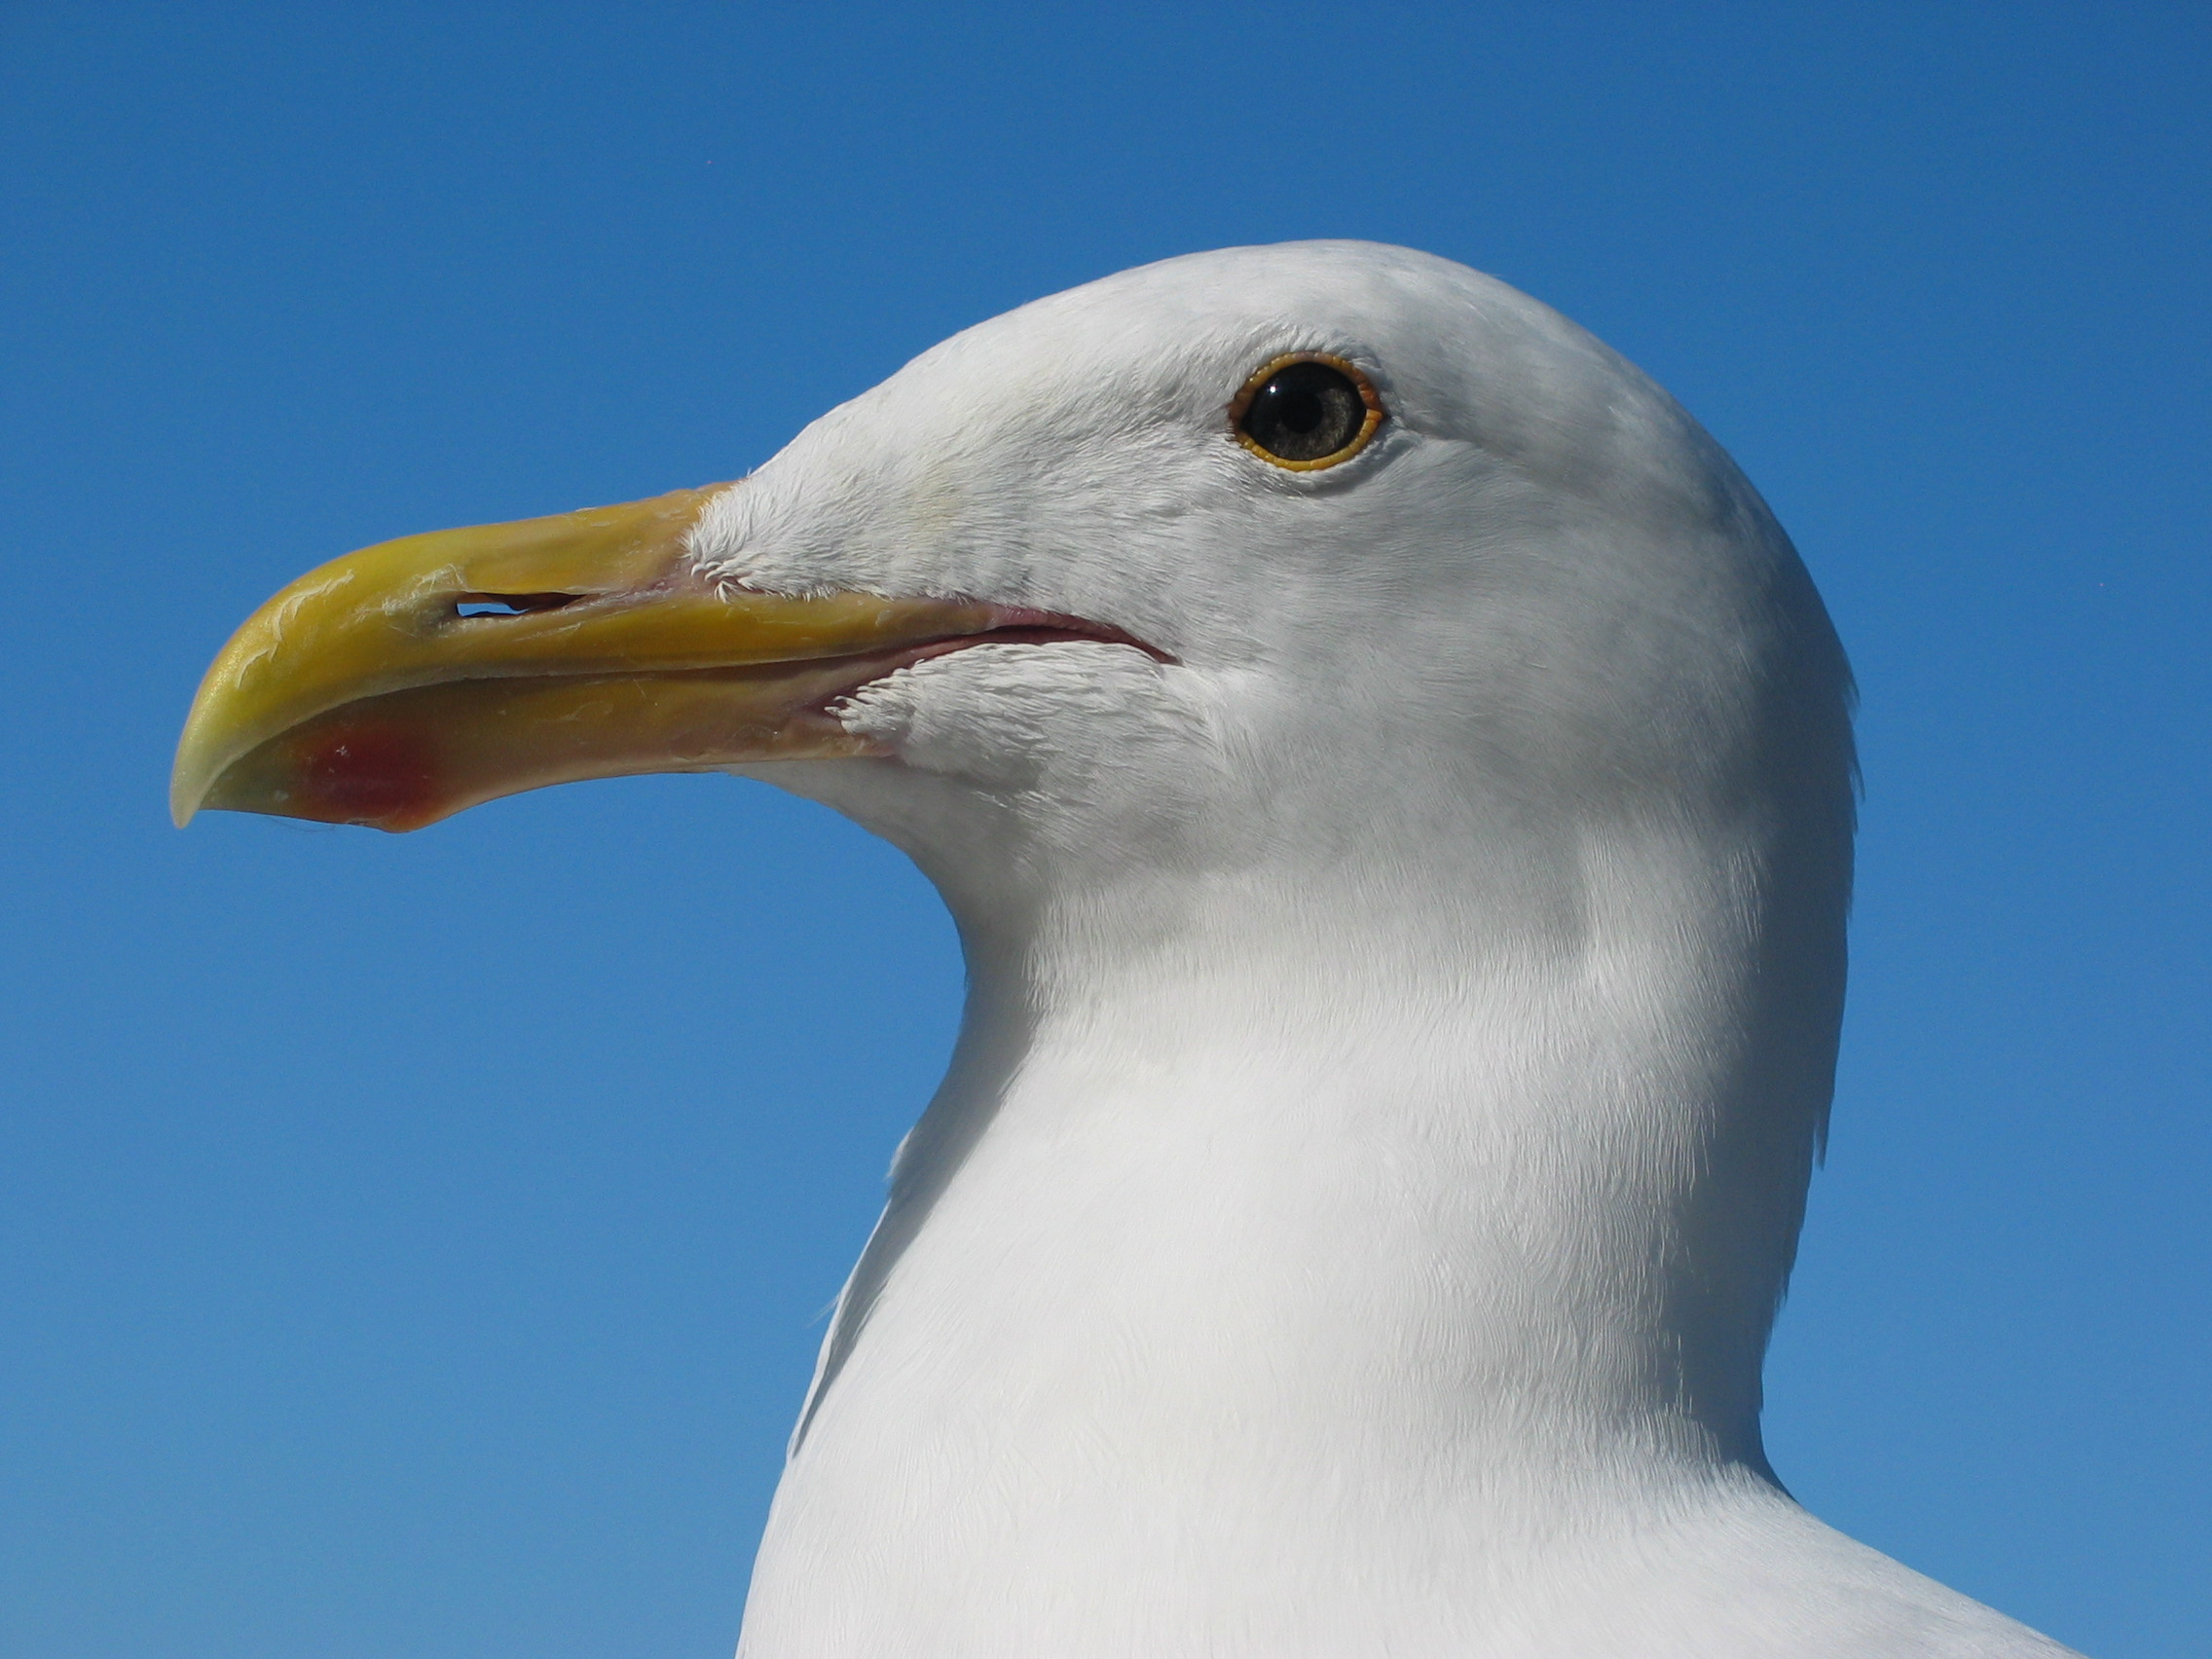
\includegraphics[width=0.48\textwidth]{gull}
  \end{center}
  \caption{A gull}
\end{wrapfigure}

They are in general medium to large birds, typically grey or white,
often with black markings on the head or wings. They have stout,
longish bills and webbed feet.

Most gulls, particularly Larus species, are ground nesting carnivores,
which will take live food or scavenge opportunistically. The live food
often includes crabs and small fish. Apart from the kittiwakes, gulls
are typically coastal or inland species, rarely venturing far out to sea.
The large species take up to four years to attain full adult plumage,
but two years is typical for small gulls.

Gulls---the larger species in particular---are resourceful and
highly intelligent birds, demonstrating complex methods of communication
and a highly developed social structure. Certain species (e.g. the
Herring Gull) have exhibited tool use behaviour. Many species of gull have
learned to co-exist successfully with man and have thrived in human habitats.
Others rely on kleptoparasitism to get their food.

\newpage
\section{RTL}

\setRTL
\subsection*{Wrapfig test}


Gulls are birds in the family Laridae. They are most closely
 related to the terns (family Sternidae), auks and skimmers,
and more distantly to the waders. Most gulls belong to the
large genus Larus.

\begin{wrapfigure}{l}{0.5\textwidth}
  \begin{center}
    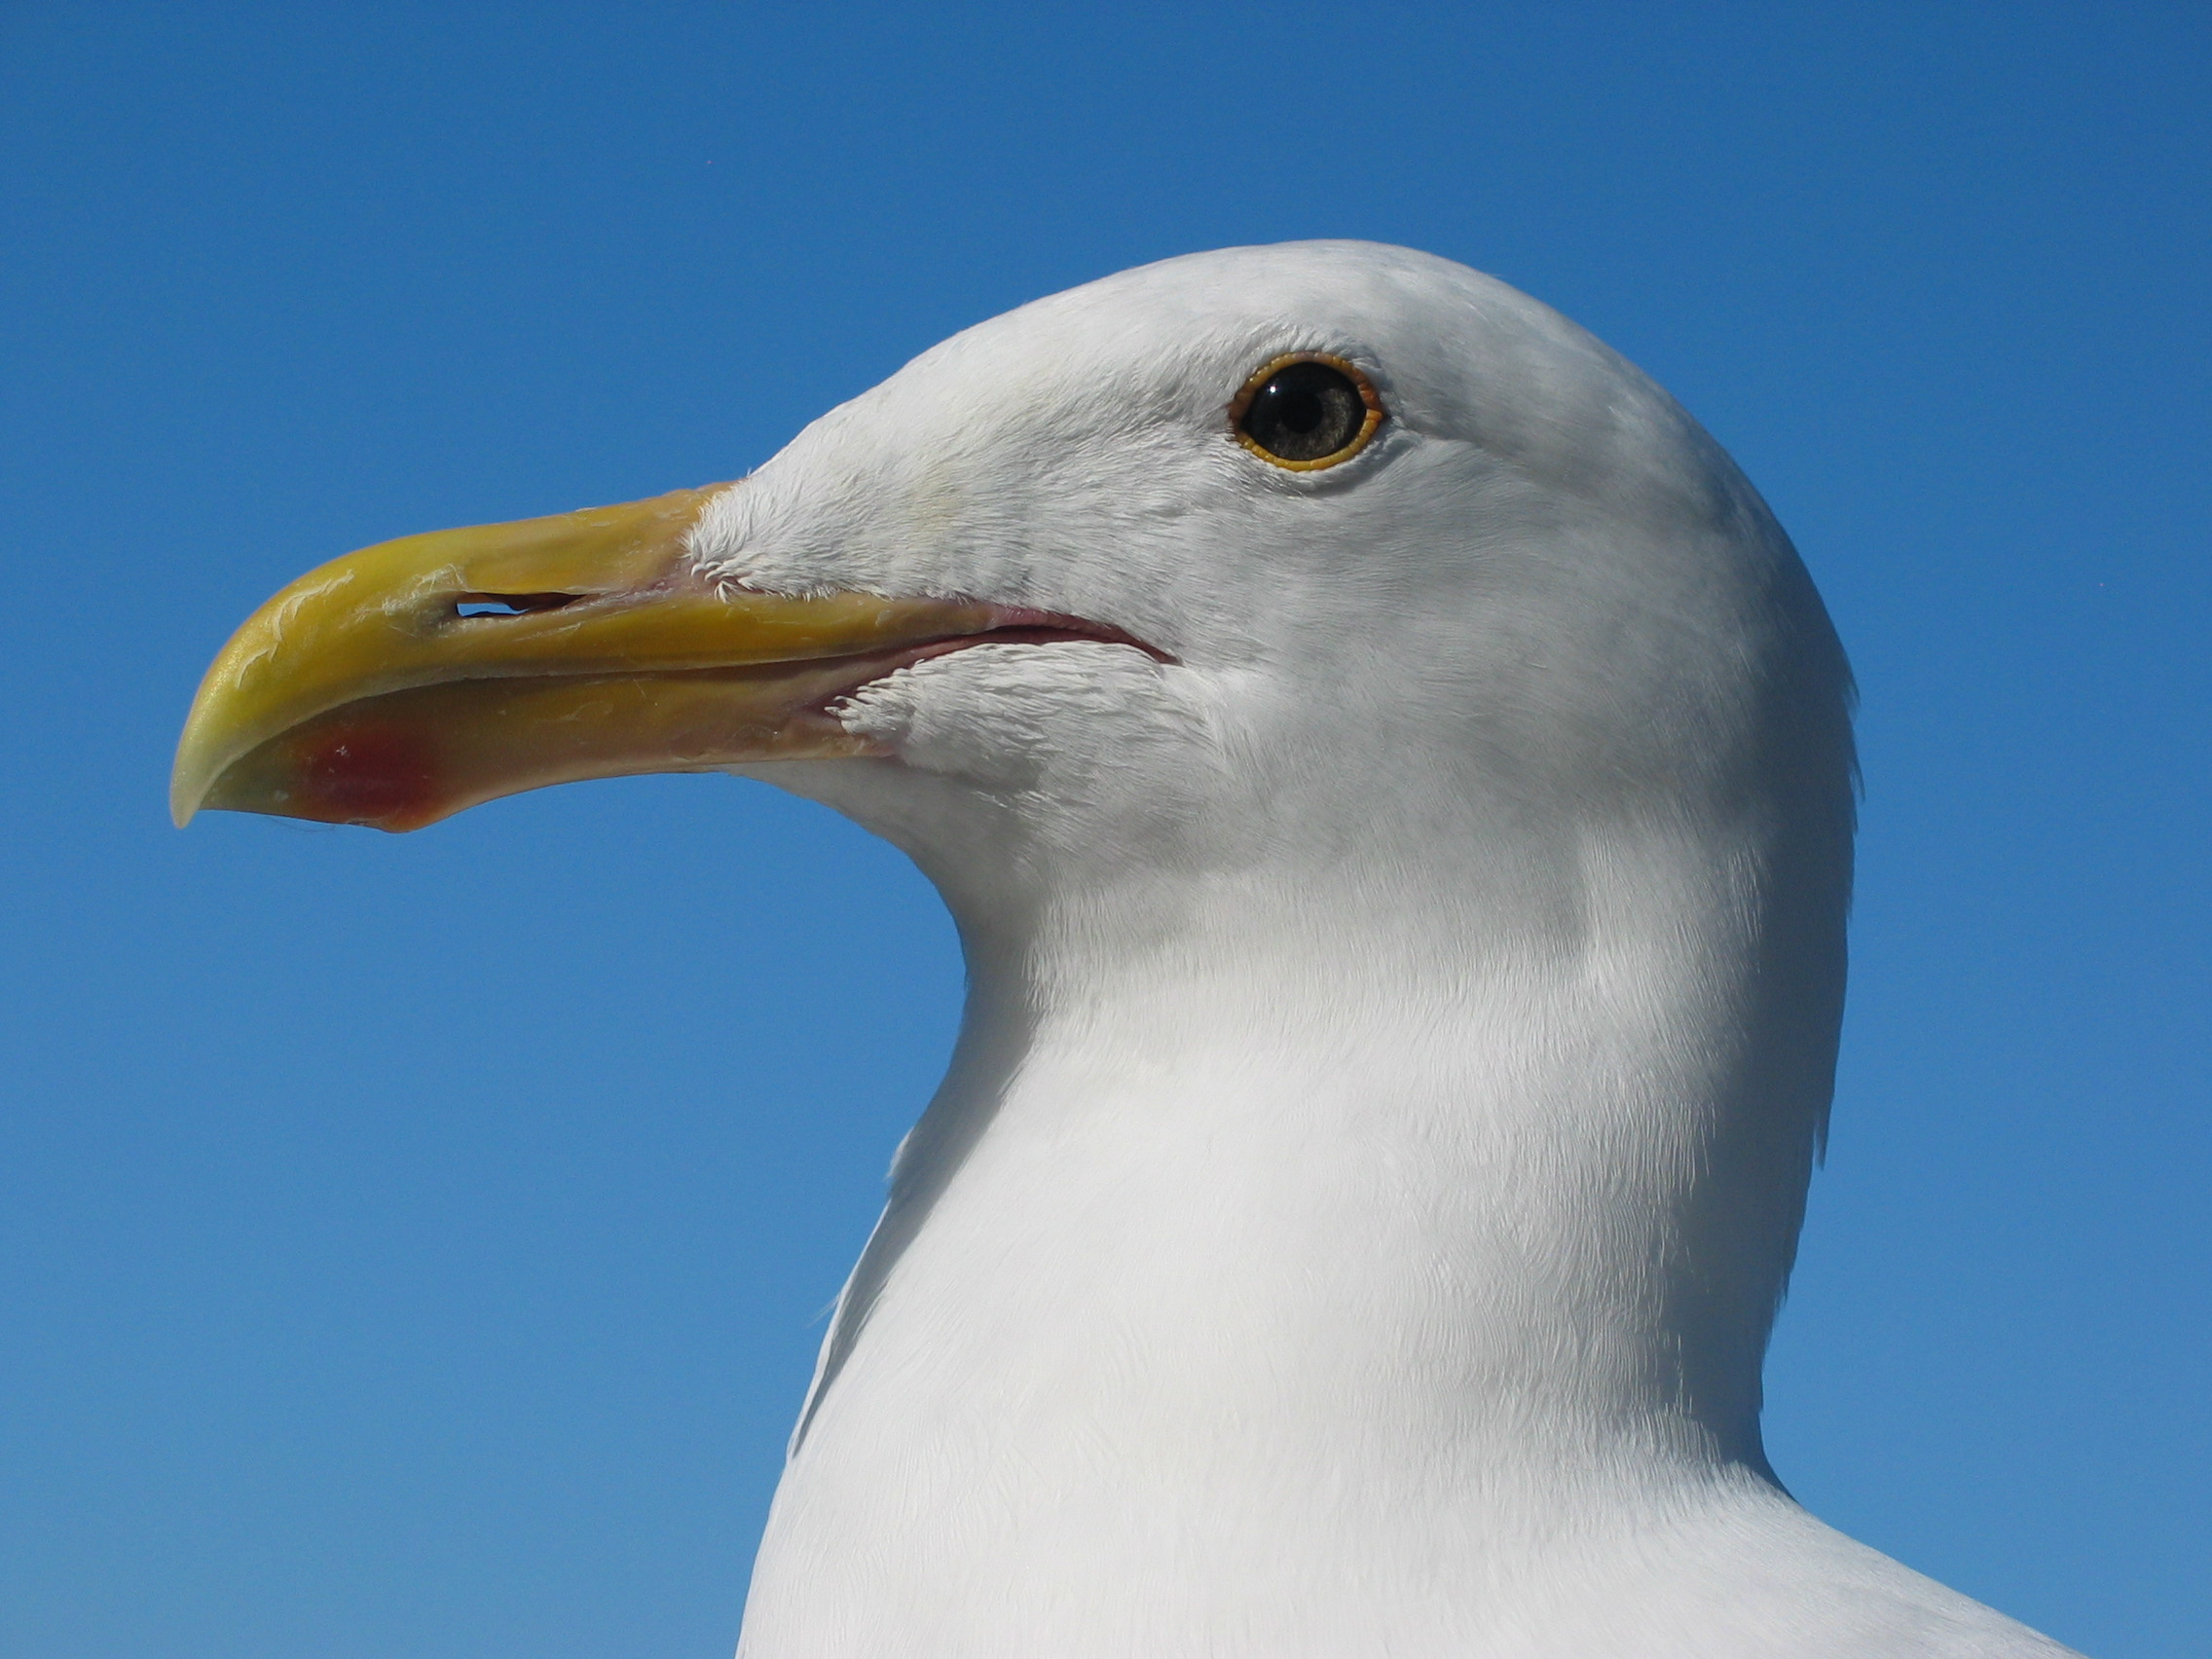
\includegraphics[width=0.48\textwidth]{gull}
  \end{center}
  \caption{A gull}
\end{wrapfigure}

They are in general medium to large birds, typically grey or white,
often with black markings on the head or wings. They have stout,
longish bills and webbed feet.

Most gulls, particularly Larus species, are ground nesting carnivores,
which will take live food or scavenge opportunistically. The live food
often includes crabs and small fish. Apart from the kittiwakes, gulls
are typically coastal or inland species, rarely venturing far out to sea.
The large species take up to four years to attain full adult plumage,
but two years is typical for small gulls.

Gulls---the larger species in particular---are resourceful and
highly intelligent birds, demonstrating complex methods of communication
and a highly developed social structure. Certain species (e.g. the
Herring Gull) have exhibited tool use behaviour. Many species of gull have
learned to co-exist successfully with man and have thrived in human habitats.
Others rely on kleptoparasitism to get their food.
\end{document}
%</test3-wrapfig.tex>
%<*test-arydshln.tex>
\documentclass{article}
\usepackage{arydshln}
\usepackage{bidi}
\title{Testing \textsf{arydshln} Package in LTR and RTL modes}
\author{}
\date{}
\begin{document}
\maketitle
\section{LTR Mode}
\begin{center}
\begin{tabular}{|l::c;{2pt/2pt}r|}\hline
A&B&C\\\hdashline[1pt/1pt]
AAA&BBB&CCC\\\cdashline{1-2}[.4pt/1pt]
\multicolumn{2}{|l;{2pt/2pt}}{AB}&C\\\hdashline\hdashline
\end{tabular}
\end{center}
\section{RTL Mode}
\begin{RTL}
\begin{center}
\begin{tabular}{|r::c;{2pt/2pt}l|}\hline
A&B&C\\\hdashline[1pt/1pt]
AAA&BBB&CCC\\\cdashline{1-2}[.4pt/1pt]
\multicolumn{2}{|r;{2pt/2pt}}{AB}&C\\\hdashline\hdashline
\end{tabular}
\end{center}
\end{RTL}
\end{document}
%</test-arydshln.tex>
%<*test-bidi.tex>
\documentclass{article}
\usepackage{bidi}
\title{Testing Basic Bidi Direction Change}
\author{Vafa Khalighi}
\begin{document}
\maketitle
In this document we test bidi direction change in \textsf{RTL} and \textsf{LTR}. These tests includes \texttt{flushleft}, \texttt{flushright} environments and \verb|\centerline{...}|, \verb|\leftline{...}|,\verb|\rightline{...}|,\verb|\raggedleft| and \verb|\raggedright| macros.
\section{RTL Test}
\setRTL
\begin{flushleft}
This is left in RTL
\end{flushleft}
\begin{flushright}
This is right in RTL
\end{flushright}
\centerline{This is center in RTL}

\leftline{This is left in RTL}

\rightline{This is right in RTL}

\raggedleft This is raggedleft in RTL

\raggedright This is raggedright in RTL

\setLTR
\section{LTR Test}
\begin{flushleft}
This is left in LTR
\end{flushleft}
\begin{flushright}
This is right in LTR
\end{flushright}
\centerline{This is center in LTR}

\leftline{This is left in LTR}

\rightline{This is right in LTR}

\raggedleft This is raggedleft in LTR

\raggedright This is raggedright in LTR
\end{document}
%</test-bidi.tex>
%<*test-brochure.tex>
\documentclass[a4paper]{report}

\usepackage[landscape,margin=1in]{geometry}
\usepackage{color}
\usepackage[RL]{flowfram}% we enable `RL' option for RTL multicolumn typesetting (see flowfram package documentation)
\usepackage[colorlinks,setpagesize=false]{hyperref}

\usepackage[RTLdocument]{bidi}
% adjust \textheight so that it is an integer multiple of
% \baselineskip
\adjustheight{\textheight}

% set up pagelayout. One column for title page
% two columns for the rest.
\onecolumninarea[1,2]{0.6\textwidth}{\textheight}{0.4\textwidth}{0pt}
\twocolumninarea[>2]{0.6\textwidth}{\textheight}{0.4\textwidth}{0pt}

% Set up dynamic frame on the left. This is where
% the headings will go.

\newdynamicframe{0.4\textwidth}{\textheight}{0pt}{0pt}[left]

% put the chapter headings in this frame
\dfchaphead*{left}
% Modify the default style
\renewcommand{\DFchapterstyle}[1]{%
\raggedright\Huge\slshape\MakeUppercase{#1}\par}

% Make static frames for background (only for page 1)
\vtwotone[1]{0.6\paperwidth}{[cmyk]{0.65,0.13,0,0}}{backleft}%
{0.4\paperwidth}{[cmyk]{0.94,0.54,0,0}}{backright}

% Make a border along the top of each page
\vtwotonetop{1cm}{0.6\paperwidth}{[cmyk]{0.65,0.13,0,0}}{topleft}%
{0.4\paperwidth}{[cmyk]{0.94,0.54,0,0}}{topright}

% make a static frame for the logo
\newstaticframe{0.2\textwidth}{0.25\textheight}{0pt}{0pt}[logo]

% empty page style, because I am going to make my own
\pagestyle{empty}

% Each new chapter sets \thispagestyle{\chapterfirstpagestyle}, change this empty as well
\renewcommand{\chapterfirstpagestyle}{empty} 

% Now make a frame in which to put my own customized footer
\newdynamicframe[>1]{\textwidth}{\headheight}{0pt}{-\footskip}[footer]

% set the contents of the frame:
\setdynamiccontents*{footer}{%
School of Computing Sciences, University of East Anglia\hfill
http://www.cmp.uea.ac.uk/\hfill
page \thepage\ of \pageref*{lastpage}}


\newcommand{\env}[1]{\texttt{#1}}
\newcommand{\cmdname}[1]{\texttt{\symbol{92}#1}}
\newcommand{\meta}[1]{\textnormal{\textless\textit{#1}\textgreater}}

\begin{document}

% not a very interesting logo
\setstaticcontents*{logo}{\sffamily{\Huge\slshape FLF} Flowfram}

{\noindent
\slshape\Huge\MakeUppercase{A Sample Brochure}\par
\vskip0.5in
\noindent\large\MakeUppercase{Nicola Talbot}\\
}


\chapter{Introduction}

The \textsl{flowfram} package is designed to enable you to create
frames in a document such that the 
contents of the \env{document} environment flow from one 
frame to the next in the order that they were defined.  
This is useful for creating posters
or magazines or any other form of document that does not 
conform to the standard one or two column layout.

This is a modified version of the manual for the \textsl{flowfram} package.
It is intended to illustrated what can be done. See the full 
manual (ffuserguide.pdf) for
a comprehensive description, as some parts of this document
may now be out of date.
If the columns are very narrow, it may be better to
use \cmdname{raggedright}, otherwise \TeX\ may have a
problem working out the line breaks.

This is column~\thedisplayedframe.

The main type of frame is the flow frame. This is described on
column~\ref{flow:flowframe} on page~\pageref{flow:flowframe}.
The order used to draw the contents of each frame on the page
is described in column~\ref{flow:stacking} on 
page~\pageref{flow:stacking}. Floats are describe in 
column~\ref{flow:floats} on page~\pageref{flow:floats}.

\chapter{Setting up Frames}

This is column~\thedisplayedframe.

The \textsl{flowfram} package provides three types of frame:
{flow frames}, {static 
frames} and {dynamic frames}.

\section*{Flow Frames}

\labelflow{flow:flowframe}
The flow frame is the principle type of frame.
The text of the \env{document} environment will flow from 
one frame to the next in order of definition. Each 
flow frame has an associated width, height, 
position on the page, and optionally a border.

It is recommended that all the flow frames in a document
have the same width, otherwise problems may occur
when a paragraph spans to flow frames of unequal
widths. This is because \TeX's output routine does not
register the change in \cmdname{hsize} until it reaches
a paragraph break. If it is absolutely necessary for 
flow frames to have unequal widths, judicious use of
\cmdname{framebreak} is required.

\section*{Static Frames}

A static frame is a rectangular area in which text neither
flows into, nor flows out of.  The contents must be set
explicitly, and once set, the contents of the static frame will
remain the same on each page until it is explicitly 
changed.  Thus, a static frame can be used, for example, to make 
a company logo appear in the same place on every page.

\section*{Dynamic Frames}

A dynamic frame is similar to a static frame, but its contents
are re-typeset on each page. (A static frame stores its 
contents in a savebox, whereas a dynamic frame stores its
contents in a macro).

This is column~\thedisplayedframe.

\chapter{Frame Attributes}
\label{sec:modattr}

Once you have defined the {flow frames}, {static frames} and 
{dynamic frames}, their attributes can be changed. 
The three types of frame mostly have the 
same set of attributes, but some are specific to a certain type.
The available attributes are as follows
(\textsuperscript{\textbf{F}} indicates the key is
only available for {flow frames}, 
\textsuperscript{\textbf{S}} indicates the key is only available 
for {static frames}
and \textsuperscript{\textbf{D}} indicates the key
is only available for {dynamic frames}):

\begin{description}
\item[width=\meta{length}]\mbox{}\par  The width of the frame.

\item[height=\meta{length}]\mbox{}\par The height of the frame.

\item[x=\meta{length}]\mbox{}\par The x-coordinate of the frame.

\item[y=\meta{length}]\mbox{}\par The y-coordinate of the frame.

\item[border=\meta{style}]\mbox{}\par The style of the border around the 
frame, this can take the values: \texttt{none} (no border),
\texttt{plain} (plain border) or the name of a \LaTeX\ 
frame making command without the preceding backslash. 
The value \texttt{fbox} is equivalent to \texttt{plain}.

\item[offset=\meta{offset}]\mbox{}\par The border offset, if it is a 
user-defined border.  This is the distance from the outer
edge of the left hand border to the left edge of the
bounding box of the text inside the border.  The \textsl{flowfram}
package is able to compute the border for 
known frame making commands. 
If you define your own frame making command, you may need to 
specify the offset explicitly, or the frames 
may end up shifted to the right or left.

\item[bordercolor=\meta{colour}]\mbox{}\par The colour of the border
if you are using a standard frame making command.
The colour can either be specified as, e.g.\ \texttt{green},
or including the colour model, for example 
\verb/[rgb]{0,1,0}/.

\item[textcolor=\meta{colour}]\mbox{}\par The text colour for that 
frame. Again, the colour can either be specified as, 
e.g.\ \texttt{green}, or including the colour model, 
for example \verb/[rgb]{0,1,0}/.

\item[pages=\meta{page list}]\mbox{}\par The {list of 
pages} for which the frame
should appear. This can either have the values: \texttt{all},
\texttt{even}, \texttt{odd} or \texttt{none} (the latter 
removes the frame from that point on---useful if you
have multiple pages with the same number), or it can be a 
comma-separated list of single pages, or 
{page ranges}.

\item[margin=\meta{side}\textsuperscript{F}]\mbox{}\par The side of
the flow frame that its corresponding margin should go on. This
can take the values \texttt{left} or \texttt{right}.

\item[clear=\meta{boolean}\textsuperscript{S}] If this value
is set, the static frame will be cleared at the start of the
next page.

\item[style=\meta{cmd}\textsuperscript{D}]\mbox{}\par This should be
the name of a command \emph{without} the preceding backslash, 
to be applied to the contents of the specified dynamic frame. 
The command may either be a declaration, for example \verb/style=large/
which will set the contents of all the dynamic frames in a
large font, or it can be a command that takes a single argument,
for example \verb/style=textbf/
which will make the text for all the dynamic frames come out in 
bold.  To unset a style, do \verb/style=none/.

\end{description}

\chapter{Miscellaneous}

\section*{Page Layout}

The \textsl{flowfram} package has the package option \texttt{draft}
which will draw the {bounding boxes} for
each frame defined.  At the bottom right of each
bounding box (except for the bounding box denoting the 
typeblock), a marker will be shown to indictate the type
of frame, its IDN and its IDL.

You can see the layout for the current page (irrespective of
whether or not the \texttt{draft} option has been set) using
the command:\newline 
\cmdname{flowframeshowlayout}

The headers and footers will appear as usual (but will not
be shown in draft mode), according to the format given by 
\cmdname{pagestyle}.

\section*{Frame Stacking Order}

\labelflow{flow:stacking}
The material on each page is placed in the following order:
\begin{enumerate}
\item Each static frame defined for that page in ascending
order of IDN.

\item Each flow frame defined for that page in ascending
order of IDN.

\item Each dynamic frame defined for that page in ascending
order of IDN.

\item {Bounding boxes} if the \texttt{draft}
package option has been used.
\end{enumerate}

This ordering can be used to determine if you want something
to overlay or underlay everything else on the page. 

\section*{Prematurely Ending a Flow Frame}

You can force text to move immediately to the next defined
flow frame using one of the standard \LaTeX\ page breaking commands
which  work in an analogous way to the way they
work in standard two column mode. 

The command \cmdname{framebreak} is provided for situations
where a paragraph spans two flow frames
of different widths, as \TeX's output routine does not 
adjust to the new value of \cmdname{hsize} until the last 
paragraph of the previous frame has ended. As a 
result, the end of the paragraph at the beginning of the new
flow frame retains the width of the previous flow frame.

If you want to start a new page, rather than simply move to the 
next frame, use the command\newline
\cmdname{finishthispage}.

\section*{Floats}

\labelflow{flow:floats}
Since floats (such as figures and tables) can only go in 
{flow frames}, this package provides
the additional environments: 
\env{staticfigure} and  
\env{statictable} which can be used in static frames
and dynamic frames. Unlike their \env{figure} and
\env{table} counterparts, they are fixed in place, and
so do not take an optional placement specifier. The 
\cmdname{caption} and \cmdname{label} commands can 
be used within \env{staticfigure} and \env{statictable} as
usual.

The standard \env{figure} and \env{table} commands will 
behave as usual in the flow frames, but their starred versions,
\env{figure*} and \env{table*} behave no differently
from \env{figure} and \env{table}.

\section*{Global Values}

The following macros can be changed using\linebreak \cmdname{renewcommand}:

\begin{itemize}
\item \cmdname{setffdraftcolor} 

This sets the colour of the bounding box
when it is displayed in draft mode.

\item 
\cmdname{setffdrafttypeblockcolor} 

This sets the colour of
the bounding box of the typeblock when it is displayed
in draft mode.

\item \cmdname{fflabelfont}

This sets the font size for the bounding box markers in 
draft mode.

\end{itemize}

The following are lengths, which can be changed using
\cmdname{setlength}:

\begin{itemize}
\item \cmdname{fflabelsep}

This is the distance from the right hand side of the
bounding box at which to place the bounding box marker.

\item \cmdname{flowframesep}

This is the gap between the text of the frame and
its border, for the standard border types. 

\item \cmdname{flowframerule}

This is the width of the frame's border, if using
a border given by a frame making command that uses \cmdname{fboxsep}
to set its border width.

\item \cmdname{columnsep}

This is the horizontal distance between flow frames when using one of the
\cmdname{Ncolumn} type of commands

\item \cmdname{vcolumnsep}

This is the vertical distance between the flow frames and the static or
dynamic frame when using one of the \cmdname{Ncolumntop} type of commands.
\end{itemize}

\label{lastpage}
\end{document}
%</test-brochure.tex>
%<*test-casualcv.tex>
\documentclass[11pt,a4paper]{bidimoderncv}
\cvtheme[orange]{bidicasual} % you can use orange, red, green and blue as options
\usepackage[scale=0.8]{geometry}
\usepackage{fontspec}
\usepackage[RTLdocument]{bidi}
\def\refname{تألیفات}
\setmainfont[Script=Arabic,Mapping=parsidigits]{XB Niloofar}
\newfontfamily\rmfamily[Mapping=tex-text]{Linux Libertine}
\AtBeginDocument{\recomputelengths}
\resumename{رزومه}
\firstname{سید محمد}
\familyname{یزدی اصفهانی}
\title{رزومهٔ من}
\address{تهران، خیابان آزادی پلاک ۹}
\mobile{۰۹۱۸۹۶۹۴۹۶}
\phone{۹۸۹۰۸۳۴۱}
\fax{۹۸۹۰۸۳۴۲}
\email{me@somedomain.com}
\extrainfo{اطلاعات اضافی}
\photo[64pt]{picture}
\quote{نقل قول}
\begin{document}
\maketitle
\section{تحصیلات}
\cventry{سال--سال}{درجه}{دانشگاه}{شهر}{\textit{نمره}}{توضیح}   % arguments 3 to 6 are optional
\cventry{سال--سال}{درجه}{دانشگاه}{شهر}{\textit{نمره}}{توضیح}  % arguments 3 to 6 are optional

\section{پایان‌نامهٔ کارشناسی ارشد}
\cvline{عنوان}{\emph{عنوان}}
\cvline{استاد راهنما}{استاد راهنما}
\cvline{توضیح}{\small چکیده کوچک پایان‌نامه}

\section{تجربیات}
\subsection{عنوان}
\cventry{سال--سال}{نام شغل}{صاحب کار}{شهر}{}{توضیح}                % arguments 3 to 6 are optional
\cventry{سال--سال}{نام شغل}{صاحب کار}{شهر}{}{توضیح}                % arguments 3 to 6 are optional
\subsection{متفرقه}
\cventry{سال--سال}{نام شغل}{صاحب کار}{شهر}{}{توضیح خط ۱\newline{}توضیح خط ۲}% arguments 3 to 6 are optional

\section{زبانها}
\cvlanguage{زبان ۱}{درجه مهارت}{نظر}
\cvlanguage{زبان ۲}{درجه مهارت}{نظر}
\cvlanguage{زبان ۳}{درجه مهارت}{نظر}

\section{مهارتهای رایانه‌ای}
\cvcomputer{طبقه ۱}{یک، دو، سه}{طبقه ۴}{یک، دو، سه}
\cvcomputer{طبقه ۲}{یک، دو، سه}{طبقه ۵}{یک، دو، سه}
\cvcomputer{طبقه ۳}{یک، دو، سه}{طبقه ۶}{یک، دو، سه}

\section{علاقه‌ها}
\cvline{علاقه ۱}{\small توضیح}
\cvline{علاقه ۲}{\small توضیح}
\cvline{علاقه ۳}{\small توضیح}

\renewcommand{\listitemsymbol}{-} % change the symbol for lists

\section{بعدی ۱}
\cvlistitem{شماره ۱}
\cvlistitem{شماره ۲}
\cvlistitem[+]{شماره ۳}            % optional other symbol

\section{بعدی ۲}
\cvlistdoubleitem[\Neutral]{شماره ۱}{شماره ۴}
\cvlistdoubleitem[\Neutral]{شماره ۲}{شماره ۵}
\cvlistdoubleitem[\Neutral]{شماره ۳}{}

\nocite{*}
\bibliographystyle{plain}
\bibliography{publications}       % 'publications' is the name of a BibTeX file

\end{document}
%</test-casualcv.tex>
%<*test-classiccv.tex>
\documentclass[11pt,a4paper]{bidimoderncv}
\cvtheme[green]{bidiclassic} % you can use orange, red, green, grey and blue as options
\usepackage[scale=0.8]{geometry}
\usepackage{fontspec}
\setmainfont[Script=Arabic,Mapping=parsidigits]{XB Zar}
\newfontfamily\rmfamily[Mapping=tex-text]{Linux Libertine}
\def\refname{تألیفات}
\usepackage[RTLdocument]{bidi}
\AtBeginDocument{\recomputelengths}
\resumename{رزومه}
\firstname{وفا}
\familyname{خلیقی}
\title{رزومهٔ من}
\address{تهران، خیابان آزادی پلاک ۹}
\mobile{۰۹۱۸۹۶۹۴۹۶}
\phone{۹۸۹۰۸۳۴۱}
\fax{۹۸۹۰۸۳۴۲}
\email{me@somedomain.com}
\extrainfo{اطلاعات اضافی}
\photo[64pt]{picture}
\quote{نقل قول}
\begin{document}
\maketitle
\section{تحصیلات}
\cventry{سال--سال}{درجه}{دانشگاه}{شهر}{\textit{نمره}}{توضیح}   % arguments 3 to 6 are optional
\cventry{سال--سال}{درجه}{دانشگاه}{شهر}{\textit{نمره}}{توضیح}  % arguments 3 to 6 are optional

\section{پایان‌نامهٔ کارشناسی ارشد}
\cvline{عنوان}{\emph{عنوان}}
\cvline{استاد راهنما}{استاد راهنما}
\cvline{توضیح}{\small چکیده کوچک پایان‌نامه}

\section{تجربیات}
\subsection{عنوان}
\cventry{سال--سال}{نام شغل}{صاحب کار}{شهر}{}{توضیح}                % arguments 3 to 6 are optional
\cventry{سال--سال}{نام شغل}{صاحب کار}{شهر}{}{توضیح}                % arguments 3 to 6 are optional
\subsection{متفرقه}
\cventry{سال--سال}{نام شغل}{صاحب کار}{شهر}{}{توضیح خط ۱\newline{}توضیح خط ۲}% arguments 3 to 6 are optional

\section{زبانها}
\cvlanguage{زبان ۱}{درجه مهارت}{نظر}
\cvlanguage{زبان ۲}{درجه مهارت}{نظر}
\cvlanguage{زبان ۳}{درجه مهارت}{نظر}

\section{مهارتهای رایانه‌ای}
\cvcomputer{طبقه ۱}{یک، دو، سه}{طبقه ۴}{یک، دو، سه}
\cvcomputer{طبقه ۲}{یک، دو، سه}{طبقه ۵}{یک، دو، سه}
\cvcomputer{طبقه ۳}{یک، دو، سه}{طبقه ۶}{یک، دو، سه}

\section{علاقه‌ها}
\cvline{علاقه ۱}{\small توضیح}
\cvline{علاقه ۲}{\small توضیح}
\cvline{علاقه ۳}{\small توضیح}

\renewcommand{\listitemsymbol}{-} % change the symbol for lists

\section{بعدی ۱}
\cvlistitem{شماره ۱}
\cvlistitem{شماره ۲}
\cvlistitem[+]{شماره ۳}            % optional other symbol

\section{بعدی ۲}
\cvlistdoubleitem[\Neutral]{شماره ۱}{شماره ۴}
\cvlistdoubleitem[\Neutral]{شماره ۲}{شماره ۵}
\cvlistdoubleitem[\Neutral]{شماره ۳}{}

\nocite{*}
\bibliographystyle{plain}
\bibliography{publications}       % 'publications' is the name of a BibTeX file

\end{document}
%</test-classiccv.tex>
%<*test-color.tex>
\documentclass{article}
\usepackage{fontspec}
\usepackage{xecolour} % for RTL coloured texts that spans more than a line
\usepackage{fullpage}
\usepackage{colortbl}
\setmainfont[Scale=1,Script=Arabic,Mapping=farsidigits]{XB Kayhan}
\usepackage{xcolor}
\usepackage[RTLdocument]{bidi}
\begin{document}
این یک آزمایش است.

\bigskip
\fcolorbox{red}{yellow}{\begin{minipage}{0.8\textwidth}
این یک متن است که من آن را داخل یک جعبهٔ زردرنگ قرار می‌دهم. این یک متن است که من آن را داخل یک جعبهٔ زردرنگ قرار می‌دهم
\end{minipage}}

این {\color{red} رنگ قرمز} است و این هم \textcolor{blue}{رنگ آبی} است همانطور که می‌بینید.

\bigskip
من اسم خودم {\color{red}  وفا خلیقی} را با رنگ قرمز می‌نویسم.

\bigskip
من اسم خودم \textcolor{blue}{وفا خلیقی} را با رنگ آبی می‌نویسم.

\bigskip
\colorbox{yellow}{\begin{minipage}{0.8\textwidth}
این یک متن است که من آن را داخل یک جعبهٔ زردرنگ قرار می‌دهم. این یک متن است که من آن را داخل یک جعبهٔ زردرنگ قرار می‌دهم
\end{minipage}}

\bigskip
این یک پاراگراف با \blue{رنگ آبی اول است و همینطور و همینطور ما می‌توانیم از رنگاهی مختلف استفاده کنیم} و حالا
\red{این روزها حجم اخبار و مطالب مرتبط با ایران و مسایل مربوط به آن بسیار زیاد شده وابزارهایی مانند گوگل ریدر برای مرور لیست بلند بالایی از سایتها و وبلاگ های به روز شده ، بیشتر مورد استفاده قرار میگیرد.} و حالا هم
\darkred{یکی از مشکلاتی که در استفاده از گوگل ریدر داشتم، نامناسب بودن فونت فارسی آن بود. اگر چه عمده وبلاگها و سایتها از فونت تاهوما (مانند فونتی که این مطالب با آن نوشته شده است) استفاده می کنند اما تعدادی از وبلاگها از فونتهای دیگری که بعضی وقتها خیلی ریز هم هستند }استفاده می کنند که خواندن آن در گوگل ریدر بسیار دشوار است. متاسفانه در گوگل ریدر بخشی برای تغییر فونت وجود ندارد و نمیتوان نوع فونت یا اندازه مطالب آن را تغییر داد. بعد از کمی جستجو بر روی اینترنت راه حل جالبی را پیدا کردم که با کمی تغییر برای مطالب فارسی هم قابل استفاده است.
اگر از فایرفاکس برای مرور مطالب جدید در گوگل ریدر استفاده می کنید، این راه حل را باری حل این مشکل به شما پیشنهاد میکنم

\bigskip
حالا نوبت جعبه‌های رنگی است یعنی مثلاً \colorbox{red}{{\color{white}سلام}} و \fcolorbox{yellow}{red}{{\color{white}این یک متن داخل جعبه رنگی است که کمی طولانی است}}






\end{document}
%</test-color.tex>
%<*test-supertabular.tex>
\documentclass{article}
\usepackage{supertabular}
\usepackage{bidi}
\title{Testing \textsf{supertabular} package in RTL and LTR}
\author{Vafa Khalighi}
\begin{document}
\maketitle
\section{LTR}
\tablecaption{The ISOGRK3 entity set}
\tablehead
   {\bfseries Entity&\bfseries  Unicode Name&\bfseries Unicode\\ \hline}
\tabletail
   {\hline \multicolumn{3}{r}{\emph{Continued on next page}}\\}
\tablelasttail{\hline}
\begin{supertabular}{lll}
alpha              & GREEK SMALL LETTER ALPHA            & 03B1\\
beta               & GREEK SMALL LETTER BETA             & 03B2\\
chi                & GREEK SMALL LETTER CHI              & 03C7\\
Delta              & GREEK CAPITAL LETTER DELTA          & 0394\\
delta              & GREEK SMALL LETTER DELTA            & 03B4\\
epsi               & GREEK SMALL LETTER EPSILON          & 03B5\\
epsis              & GREEK LUNATE EPSILON SYMBOL         & 03F5\\
\empty
epsiv              & GREEK SMALL LETTER EPSILON          & 03B5\\
eta                & GREEK SMALL LETTER ETA              & 03B7\\
Gamma              & GREEK CAPITAL LETTER GAMMA          & 0393\\
gamma              & GREEK SMALL LETTER GAMMA            & 03B3\\
gammad             & GREEK SMALL LETTER DIGAMMA          & 03DD\\
iota               & GREEK SMALL LETTER IOTA             & 03B9\\
kappa              & GREEK SMALL LETTER KAPPA            & 03BA\\
kappav             & GREEK KAPPA SYMBOL                  & 03F0\\
Lambda             & GREEK CAPITAL LETTER LAMDA          & 039B\\
lambda             & GREEK SMALL LETTER LAMDA            & 03BB\\
mu                 & GREEK SMALL LETTER MU               & 03BC\\
nu                 & GREEK SMALL LETTER NU               & 03BD\\
Omega              & GREEK CAPITAL LETTER OMEGA          & 03A9\\
omega              & GREEK SMALL LETTER OMEGA            & 03C9\\
Phi                & GREEK CAPITAL LETTER PHI            & 03A6\\
phis               & GREEK PHI SYMBOL                    & 03D5\\
phiv               & GREEK SMALL LETTER PHI              & 03C6\\
Pi                 & GREEK CAPITAL LETTER PI             & 03A0\\
pi                 & GREEK SMALL LETTER PI               & 03C0\\
piv                & GREEK PI SYMBOL                     & 03D6\\
Psi                & GREEK CAPITAL LETTER PSI            & 03A8\\
psi                & GREEK SMALL LETTER PSI              & 03C8\\
rho                & GREEK SMALL LETTER RHO              & 03C1\\
rhov               & GREEK RHO SYMBOL                    & 03F1\\
Sigma              & GREEK CAPITAL LETTER SIGMA          & 03A3\\
sigma              & GREEK SMALL LETTER SIGMA            & 03C3\\
sigmav             & GREEK SMALL LETTER FINAL SIGMA      & 03C2\\
tau                & GREEK SMALL LETTER TAU              & 03C4\\
Theta              & GREEK CAPITAL LETTER THETA          & 0398\\
thetas             & GREEK SMALL LETTER THETA            & 03B8\\
thetav             & GREEK THETA SYMBOL                  & 03D1\\
Upsi               & GREEK UPSILON WITH HOOK SYMBOL      & 03D2\\
upsi               & GREEK SMALL LETTER UPSILON          & 03C5\\
Xi                 & GREEK CAPITAL LETTER XI             & 039E\\
xi                 & GREEK SMALL LETTER XI               & 03BE\\
zeta               & GREEK SMALL LETTER ZETA             & 03B6\\
\end{supertabular}
\section{RTL}

\setRTL
\tablecaption{The ISOGRK3 entity set}
\tablehead
   {\bfseries Entity&\bfseries  Unicode Name&\bfseries Unicode\\ \hline}
\tabletail
   {\hline \multicolumn{3}{l}{\emph{Continued on next page}}\\}
\tablelasttail{\hline}
\begin{supertabular}{rrr}
alpha              & GREEK SMALL LETTER ALPHA            & 03B1\\
beta               & GREEK SMALL LETTER BETA             & 03B2\\
chi                & GREEK SMALL LETTER CHI              & 03C7\\
Delta              & GREEK CAPITAL LETTER DELTA          & 0394\\
delta              & GREEK SMALL LETTER DELTA            & 03B4\\
epsi               & GREEK SMALL LETTER EPSILON          & 03B5\\
epsis              & GREEK LUNATE EPSILON SYMBOL         & 03F5\\
\empty
epsiv              & GREEK SMALL LETTER EPSILON          & 03B5\\
eta                & GREEK SMALL LETTER ETA              & 03B7\\
Gamma              & GREEK CAPITAL LETTER GAMMA          & 0393\\
gamma              & GREEK SMALL LETTER GAMMA            & 03B3\\
gammad             & GREEK SMALL LETTER DIGAMMA          & 03DD\\
iota               & GREEK SMALL LETTER IOTA             & 03B9\\
kappa              & GREEK SMALL LETTER KAPPA            & 03BA\\
kappav             & GREEK KAPPA SYMBOL                  & 03F0\\
Lambda             & GREEK CAPITAL LETTER LAMDA          & 039B\\
lambda             & GREEK SMALL LETTER LAMDA            & 03BB\\
mu                 & GREEK SMALL LETTER MU               & 03BC\\
nu                 & GREEK SMALL LETTER NU               & 03BD\\
Omega              & GREEK CAPITAL LETTER OMEGA          & 03A9\\
omega              & GREEK SMALL LETTER OMEGA            & 03C9\\
Phi                & GREEK CAPITAL LETTER PHI            & 03A6\\
phis               & GREEK PHI SYMBOL                    & 03D5\\
phiv               & GREEK SMALL LETTER PHI              & 03C6\\
Pi                 & GREEK CAPITAL LETTER PI             & 03A0\\
pi                 & GREEK SMALL LETTER PI               & 03C0\\
piv                & GREEK PI SYMBOL                     & 03D6\\
Psi                & GREEK CAPITAL LETTER PSI            & 03A8\\
psi                & GREEK SMALL LETTER PSI              & 03C8\\
rho                & GREEK SMALL LETTER RHO              & 03C1\\
rhov               & GREEK RHO SYMBOL                    & 03F1\\
Sigma              & GREEK CAPITAL LETTER SIGMA          & 03A3\\
sigma              & GREEK SMALL LETTER SIGMA            & 03C3\\
sigmav             & GREEK SMALL LETTER FINAL SIGMA      & 03C2\\
tau                & GREEK SMALL LETTER TAU              & 03C4\\
Theta              & GREEK CAPITAL LETTER THETA          & 0398\\
thetas             & GREEK SMALL LETTER THETA            & 03B8\\
thetav             & GREEK THETA SYMBOL                  & 03D1\\
Upsi               & GREEK UPSILON WITH HOOK SYMBOL      & 03D2\\
upsi               & GREEK SMALL LETTER UPSILON          & 03C5\\
Xi                 & GREEK CAPITAL LETTER XI             & 039E\\
xi                 & GREEK SMALL LETTER XI               & 03BE\\
zeta               & GREEK SMALL LETTER ZETA             & 03B6\\
\end{supertabular}
\end{document}
%</test-supertabular.tex>
%<*test-tabular.tex>
\documentclass{article}
\usepackage{bidi}
\title{Testing \LaTeX's Default Tabular in \textsf{RTL} and \textsf{LTR}}
\author{Vafa Khalighi}
\newcommand{\rb}[1]{\raisebox{1.5ex}[0mm]{#1}}
\begin{document}
\maketitle
In this document we test \LaTeX's default tabular in \textsf{RTL} and \textsf{LTR}.
\section{LTR}
\begin{center}\small
\begin{tabular}{|l||c|l|c|l|c|l|}
\hline
& \multicolumn{2}{c|}{6.15--7.15 pm} & \multicolumn{2}{c|}{7.20--8.20 pm}
& \multicolumn{2}{c|}{8.30--9.30 pm} \\ \cline{2-7}
&& Teacher && Teacher && Teacher \\ \cline{3-3}\cline{5-5}\cline{7-7}
\rb{Day} & \rb{Subj.} & Room & \rb{Subj.} & Room & \rb{Subj.} & Room\\
   \hline\hline
&& Dr.~Smith && Ms.~Clark && Mr.~Mills\\
\cline{3-3}\cline{5-5}\cline{7-7}
\rb{Mon.} & \rb{UNIX} & Comp. Ctr & \rb{Fortran} & Hall A
  & \rb{Math.} & Hall A \\ \hline
&& Miss Baker && Ms.~Clark && Mr.~Mill\\
\cline{3-3}\cline{5-5}\cline{7-7}
\rb{Tues.} & \rb{\LaTeX} & Conf.~Room & \rb{Fortran} & Conf~Room
  & \rb{Math.} & Hall A \\ \hline
&& Dr.~Smith && Dr.~Jones && Dr.~Jones \\
\cline{3-3}\cline{5-5}\cline{7-7}
\rb{Wed.} & \rb{UNIX} & Comp. Ctr & \rb{C} & Hall A
  & \rb{ComSci.} & Hall A \\ \hline
&& Miss Baker && Ms. Clark & \multicolumn{2}{c|}{} \\
\cline{3-3}\cline{5-5}
\rb{Fri.} & \rb{\LaTeX} & Conf.~Room & \rb{C++} & Conf.~Room
& \multicolumn{2}{c|}{\rb{canceled}}\\ \hline
\end{tabular}\end{center}
\section{RTL}

\setRTL
\begin{center}\small
\begin{tabular}{|r||c|r|c|r|c|r|}
\hline
& \multicolumn{2}{c|}{6.15--7.15 pm} & \multicolumn{2}{c|}{7.20--8.20 pm}
& \multicolumn{2}{c|}{8.30--9.30 pm} \\ \cline{2-7}
&& Teacher && Teacher && Teacher \\ \cline{3-3}\cline{5-5}\cline{7-7}
\rb{Day} & \rb{Subj.} & Room & \rb{Subj.} & Room & \rb{Subj.} & Room\\
   \hline\hline
&& Dr.~Smith && Ms.~Clark && Mr.~Mills\\
\cline{3-3}\cline{5-5}\cline{7-7}
\rb{Mon.} & \rb{UNIX} & Comp. Ctr & \rb{Fortran} & Hall A
  & \rb{Math.} & Hall A \\ \hline
&& Miss Baker && Ms.~Clark && Mr.~Mill\\
\cline{3-3}\cline{5-5}\cline{7-7}
\rb{Tues.} & \rb{\LaTeX} & Conf.~Room & \rb{Fortran} & Conf~Room
  & \rb{Math.} & Hall A \\ \hline
&& Dr.~Smith && Dr.~Jones && Dr.~Jones \\
\cline{3-3}\cline{5-5}\cline{7-7}
\rb{Wed.} & \rb{UNIX} & Comp. Ctr & \rb{C} & Hall A
  & \rb{ComSci.} & Hall A \\ \hline
&& Miss Baker && Ms. Clark & \multicolumn{2}{c|}{} \\
\cline{3-3}\cline{5-5}
\rb{Fri.} & \rb{\LaTeX} & Conf.~Room & \rb{C++} & Conf.~Room
& \multicolumn{2}{c|}{\rb{canceled}}\\ \hline
\end{tabular}\end{center}
\end{document}
%</test-tabular.tex>
%<*test-tabularx.tex>
\documentclass{article}
\usepackage{tabularx}
\usepackage{bidi}
\title{Testing \textsf{tabularx} Package in RTL and LTR}
\author{Vafa Khalighi}
\begin{document}
\maketitle
\section{LTR}
\begin{tabularx}{\linewidth}{|l|p{1.25cm}|p{1.5cm}|X|}\hline
\multicolumn{1}{|c|}{\textbf{Animal}}
  & \textbf{Hair Colour}
  & \multicolumn{2}{c|}{\textbf{Favourite foods}} \\\hline\hline
Elephant & Gray & Peanuts
  & Unshelled, prepared in Sea Salt, and warmed over hot stone grill \\\cline{3-4}
  &  & Cabbage and Greens
  & Sun dried until lightly browned (2-3 days minimum);
    seasoned with Hyperchem super feed \\\cline{4-4}
  & & & Boiled to British standard \\\hline\hline
Lion & Yellow & Elephants & Tartare \\\cline{4-4}
& & & Must be served warm, with no trace of
  buckshot. Gaiminess considered desireable. \\\hline
\end{tabularx}
\section{RTL}

\setRTL
\begin{tabularx}{\linewidth}{|r|p{1.25cm}|p{1.5cm}|X|}\hline
\multicolumn{1}{|c|}{\textbf{Animal}}
  & \textbf{Hair Colour}
  & \multicolumn{2}{c|}{\textbf{Favourite foods}} \\\hline\hline
Elephant & Gray & Peanuts
  & Unshelled, prepared in Sea Salt, and warmed over hot stone grill \\\cline{3-4}
  &  & Cabbage and Greens
  & Sun dried until lightly browned (2-3 days minimum);
    seasoned with Hyperchem super feed \\\cline{4-4}
  & & & Boiled to British standard \\\hline\hline
Lion & Yellow & Elephants & Tartare \\\cline{4-4}
& & & Must be served warm, with no trace of
  buckshot. Gaiminess considered desireable. \\\hline
\end{tabularx}
\end{document}
%</test-tabularx.tex>
%<*test-tabulary.tex>
\documentclass{article}
\usepackage{tabulary}
\setlength\tymin{10pt}
\setlength\tymax{\maxdimen}
\usepackage{bidi}
\title{Testing \textsf{tabulary} package in RTL and LTR}
\author{Vafa Khalighi}
\begin{document}
\maketitle
\section{LTR}
\begin{tabulary}{200pt}{|C|C|C|C|}
 a & b b b b &
 c c c c c c c c c c c c c c c c c c &
 d d d d d d d d d d d d d d d d d d
\empty
 d d d d d d d d d d d d d d
 d d d d d d d d d d d d d d d d d d d d d d d d d d d d d d d d
 \end{tabulary}
\section{RTL}

\setRTL
\begin{tabulary}{200pt}{|C|C|C|C|}
 a & b b b b &
 c c c c c c c c c c c c c c c c c c &
 d d d d d d d d d d d d d d d d d d
\empty
 d d d d d d d d d d d d d d
 d d d d d d d d d d d d d d d d d d d d d d d d d d d d d d d d
 \end{tabulary}
\end{document}
%</test-tabulary.tex>
%\fi
%
% \typeout{*************************************************************}
% \typeout{*}
% \typeout{* To finish the installation you have to move the following}
% \typeout{* file into a directory searched by TeX:}
% \typeout{*}
% \typeout{* \space\space\space all *.cls, *.sty and *.def  files}
% \typeout{*}
% \typeout{* \space\space\space and bidi-bibitem.pdf  file}
% \typeout{*************************************************************}
%
\endinput

